\documentclass[twosided,12pt]{book}

\usepackage{mathptmx}
\usepackage[T1]{fontenc}
\usepackage{roboto} %%for Lyryx Icon font

\usepackage{amssymb}
\usepackage{amsmath}
\usepackage{amsthm}

% Make it look more like the Word docs
\setlength{\parskip}{\baselineskip}
\setlength{\parindent}{0pt}

% Coloring various things
\usepackage[usenames,dvipsnames,table]{xcolor}

% Conditional statements
\usepackage{ifthen}

% Page layout
\ifthenelse{\equal{\detokenize{interior}}{\jobname}\or\equal{\detokenize{solutions-interior}}{\jobname}\or\equal{\detokenize{exercises-interior}}{\jobname}\or\equal{\detokenize{exercises-solutions-interior}}{\jobname}}{
	\usepackage[headheight=15pt,top=1in, bottom=1in, outer=0.75in, inner=1.25in]{geometry}
}{
	\usepackage[headheight=15pt,top=1in, bottom=1in, outer=1in, inner=1in]{geometry}
}

% Figures that don't float
\usepackage{float}

% Used to define new float type for Application Boxes
\usepackage{newfloat}

% For more caption features. The options make the captions bold.
\usepackage[format=hang,font=bf]{caption}

% Better version of cline
\usepackage{hhline}

% Coloring table cells
\usepackage{colortbl}

% Colored tables and other nice enhancements
\usepackage{tabu}

% For multirow cells in tables
\usepackage{multirow}

% For multicolumn cells in tables
\usepackage{multicol}

% Accompanies titlesec for handling toc/lof/lot entries
% TODO: \usepackage{titletoc}

% Customized part, chapter, section & subsection headers
\usepackage[explicit]{titlesec}

% To prevent empty pages from having headers and footers
\usepackage{emptypage}

% Used on title page
\usepackage{pagecolor}
\usepackage{afterpage}

\usepackage{tcolorbox} %%for cover page 

% Draw frames around text
\usepackage[framemethod=tikz]{mdframed}
\mdfsetup{skipabove=\topskip,skipbelow=\topskip}

% Hyperlinks
\usepackage{hyperref}

% For simple arithmetic
\usepackage{calc}

% Draw images and figures
\usepackage{tikz}
\usetikzlibrary{calc,intersections,shapes.callouts}
\usetikzlibrary{decorations.text}
\usetikzlibrary{shapes,positioning}
\usetikzlibrary{decorations.pathreplacing}
\usetikzlibrary{shadows,trees}
\usetikzlibrary{backgrounds}

% For fancy headers!
\usepackage{fancyhdr}

% For plotting data
\usepackage{pgfplots}

\usepackage{pgfplotstable}

% Used for creating EOC questions with corresponding solutions at the end of the textbook
\usepackage{answers}

% Building a solutions manual
\ifthenelse{\equal{\detokenize{solutions}}{\jobname}\or\equal{\detokenize{exercises}}{\jobname}\or\equal{\detokenize{exercises-solutions}}{\jobname}\or\equal{\detokenize{solutions-interior}}{\jobname}\or\equal{\detokenize{exercises-interior}}{\jobname}\or\equal{\detokenize{exercises-solutions-interior}}{\jobname}}{
	\usepackage{xr}
	\externaldocument{interior}
}
{
	% Don't include...
}

% Curtis Irvine Style
\usepackage{cistyle}

% Basic book information (version, revision, name) - info that should not change with adaptations
\input{frontmatter/bookinfo.txt}

% Information regarding course (for adaptations)
\input{frontmatter/courseinfo.txt}

% Glossary
\usepackage[toc,acronym]{glossaries}

%\makeglossaries

%\newglossaryentry{accprofit}
{
	name={accounting profits},
	description={The difference between revenues and actual costs incurred}
}

\newglossaryentry{adverseselection}
{
	name={adverse selection},
	description={Occurs when incomplete or asymmetric information describes an economic relationship}
}

\newglossaryentry{affordableset}
{
	name={affordable set},
	description={Goods and services for the consumer which are bounded by the budget line from above}
}

\newglossaryentry{nonaffordableset}
{
	name={non-affordable set},
	description={Goods and services for the consumer which lie strictly above the budget line}
}

\newglossaryentry{ageearningsprofiles}
{
	name={age-earnings profile},
	description={Define the pattern of earnings over time for individuals with different characteristics}
}

\newglossaryentry{agent}
{
	name={agent},
	description={Usually a manager who works in a corporation and is directed to follow the corporation's
interests}
}

\newglossaryentry{allocativeinefficiency}
{
	name={allocative inefficiency},
	description={Arises when resources are not appropriately allocated and result in dead-weight losses}
}

\newglossaryentry{arcelasticityofdemand}
{
	name={arc elasticity of demand},
	description={Defines consumer responsiveness over a segment or \emph{arc} of the demand curve}
}

\newglossaryentry{assetprice}
{
	name={asset price},
	description={The financial sum for which the asset can be purchased}
}

\newglossaryentry{asymmetricinformation}
{
	name={asymmetric information},
	description={Is where at least one party in an economic relationship has less than full information and has a different amount of information from another party}
}

\newglossaryentry{autarky}
{
	name={autarky},
	description={Denotes the no-trade situation}
}

\newglossaryentry{averagefixedcost}
{
	name={average fixed cost},
	description={Is the total fixed cost per unit of output}
}

\newglossaryentry{averageproductoflabour}
{
	name={average product of labour},
	description={Is the number of units of output produced per unit of labour at different levels of employment}
}

\newglossaryentry{averagerevenue}
{
	name={average revenue},
	description={Is the price per unit sold}
}

\newglossaryentry{atc}
{
	name={average total cost ($ATC$)},
	description={Is the sum of all costs per unit of output}
}

\newglossaryentry{avc}
{
	name={average variable cost ($AVC$)},
	description={Is the total variable cost per unit of output}
}

\newglossaryentry{bindingcommitment}
{
	name={binding commitment},
	description={An agreement, entered into voluntarily, that restricts future actions}
}

\newglossaryentry{boom}
{
	name={boom},
	description={A period of high growth that raises output above normal capacity output}
}

\newglossaryentry{breakevenprice}
{
	name={break-even price},
	description={Corresponds to the minimum of the $ATC$ curve}
}

\newglossaryentry{budgetconstraint}
{
	name={budget constraint},
	description={Defines all bundles of goods that the consumer can afford with a given budget}
}

\newglossaryentry{capitalgains}
{
	name={capital gain (loss)},
	description={Arise from the ownership of a corporation when an individual sells a share at a price higher (lower) than when the share was purchased}
}

\newglossaryentry{capitalmarket}
{
	name={capital market},
	description={A set of financial institutions that funnels financing from investors into bonds and stocks}
}

\newglossaryentry{capitalservices}
{
	name={capital services},
	description={The production inputs generated by capital assets}
}

\newglossaryentry{capitalstock}
{
	name={capital stock},
	description={The buildings, machinery, equipment and software used in producing goods and services}
}

\newglossaryentry{cardinalutility}
{
	name={cardinal utility},
	description={A measurable concept of satisfaction}
}

\newglossaryentry{cluster}
{
	name=cluster,
	description={A group of firms producing similar products, or engaged in similar research}
}

\newglossaryentry{collusion}
{
	name=collusion,
	description={An explicit or implicit agreement to avoid competition with a view to increasing profit}
}

\newglossaryentry{comparativestaticanalysis}
{
	name={comparative static analysis},
	description={Compares an initial equilibrium with a new equilibrium, where the difference is due to a change in one of the other things that lie behind the demand curve or the supply curve}
}

\newglossaryentry{complementarygoods}
{
	name={complementary goods},
	description={When a price reduction (rise) for a related product increases (reduces) the demand for a primary product, it is a complement for the primary product}
}

\newglossaryentry{concentrationratio}
{
	name={concentration ratio},
	description={$N$-firm concentration ratio is the sales share of the largest $N$ firms in that sector of the economy}
}

\newglossaryentry{conjecture}
{
	name=conjecture,
	description={A belief that one firm forms about the strategic reaction of another competing firm}
}

\newglossaryentry{consumerequilibrium}
{
	name={consumer equilibrium},
	description={Occurs when marginal utility per dollar spent on the last unit of each good is equal}
}

\newglossaryentry{consumeroptimum}
{
	name={consumer optimum},
	description={Occurs where the chosen consumption bundle is a point such that the price ratio equals the marginal rate of substitution}
}

\newglossaryentry{consumerpriceindex}
{
	name={consumer price index},
	description={The average price level for consumer goods and services}
}

\newglossaryentry{consumersurplus}
{
	name={consumer surplus},
	description={The excess of consumer willingness to pay over the market price}
}

\newglossaryentry{consumptionpossibilityfrontier}
{
	name={consumption possibility frontier},
	description={Defines what an economy can consume after production specialization and trade}
}

\newglossaryentry{corporation}
{
	name={corporation or company},
	description={An organization with a legal identity separate from its owners that produces and trades}
}

\newglossaryentry{correctivetax}
{
	name={corrective tax},
	description={Seeks to direct the market towards a more efficient output}
}

\newglossaryentry{cournot}
{
	name={cournot behaviour},
	description={Involves each firm reacting optimally in their choice of output to their competitors' decisions}
}

\newglossaryentry{crediblethreat}
{
	name={credible threat},
	description={One that, after the fact, is still optimal to implement}
}

\newglossaryentry{crossprice}
{
	name={cross-price elasticity of demand},
	description={The percentage change in the quantity demanded of a product divided by the percentage change in the price of another}
}

\newglossaryentry{crosssection}
{
	name={cross-section data},
	description={Values for different variables recorded at a point in time}
}

\newglossaryentry{data}
{
	name=data,
	description={Recorded values of variables}
}

\newglossaryentry{deadweightloss}
{
	name={deadweight loss},
	description={The deadweight loss of a tax is the component of consumer and producer surpluses forming a net loss to the whole economy}
}

\newglossaryentry{decreasingreturntoscale}
{
	name={decreasing returns to scale},
	description={Implies that an equal proportionate increase in all inputs leads to a less than proportionate increase in output}
}

\newglossaryentry{deflationrate}
{
	name={deflation rate},
	description={The annual percentage decrease in the consumer price index}
}

\newglossaryentry{demandcurve}
{
	name={demand curve},
	description={A graphical expression of the relationship between price and quantity demanded, with other influences remaining unchanged}
}

\newglossaryentry{demandforlabour}
{
	name={demand for labour},
	description={A derived demand, reflecting the demand for the output of final goods and services}
}

\newglossaryentry{elastic}
{
	name=elastic,
	description={Demand is elastic is the price elasticity is greater than unity}
}

\newglossaryentry{inelastic}
{
	name=inelastic,
	description={Demand is inelastic if the price elasticity lies between unity and 0}
}

\newglossaryentry{unit elastic}
{
	name={unit elastic},
	description={Demand is unit elastic if the price elasticity is exactly one}
}

\newglossaryentry{demand}
{
	name=demand,
	description={The quantity of good or service that buyers wish to purchase at each possible price, with all other influences on demand remaining unchanged}
}

\newglossaryentry{depreciation}
{
	name=depreciation,
	description={The annual change in the value of physical asset}
}

\newglossaryentry{differentiatedproduct}
{
	name={differentiated product},
	description={The product that differs slightly from other products in the same market}
}

\newglossaryentry{diminishingmrs}
{
	name={diminishing marginal rate of substitution},
	description={Reflects a higher marginal value being associated with smaller quantities of any good consumed}
}

\newglossaryentry{diminishingmu}
{
	name={diminishing marginal utility},
	description={Implies that the addition to total utility from each extra unit of a good or service consumed is declining}
}

\newglossaryentry{discrimination}
{
	name=discrimination,
	description={Implies an earnings differential that is attributable to a trait other than human capital}
}

\newglossaryentry{distortion}
{
	name=distortion,
	description={In resource allocation distortion means that production is not at an efficient output, or a given output is not efficiently allocated}
}

\newglossaryentry{diversification}
{
	name=diversification,
	description={Reduces the total risk of a portfolio by pooling risks across several different assets whose individual returns behave independently}
}

\newglossaryentry{dividends}
{
	name=dividends,
	description={Payments made from after-tax profits to company shareholds}
}

\newglossaryentry{dominantstrategy}
{
	name={dominant strategy},
	description={A player's best strategy, whatever the strategies adopted by rivals}
}

\newglossaryentry{dumping}
{
	name=dumping,
	description={A predatory practice, based on artificial costs aimed at driving out domestic producers}
}

\newglossaryentry{duopoly}
{
	name=duopoly,
	description={Defines a market or sector with just two firms}
}

\newglossaryentry{econometrics}
{
	name=econometrics,
	description={The science of examining and quantifying relationships between economic variables}
}

\newglossaryentry{economicprofits}
{
	name={economic (supernormal) profits},
	description={Those profits above normal profits that induce firms to enter an industry. Economic profits are based on the opportunity cost of the resources used in production}
}

\newglossaryentry{economicefficiency}
{
	name={economic efficiency},
	description={Defines a production structure that produces output at least cost}
}

\newglossaryentry{economicequity}
{
	name={economic equity},
	description={Concerned with the distribution of well-being among members of the economy}
}

\newglossaryentry{economyscope}
{
	name={economies of scope},
	description={Occurs if the unit cost of producing particular products is less when combined with the production of other products than when produced alone}
}

\newglossaryentry{economywideppf}
{
	name={economy wide $PPF$},
	description={The set of goods combinations that can be produced in the economy when all available resources are in use}
}

\newglossaryentry{educationpremium}
{
	name={education premium},
	description={The difference in earnings between the more and less highly educated}
}

\newglossaryentry{efficiency}
{
	name=efficiency,
	description={Addresses the question of how well the economy's resources are used and allocated}
}

\newglossaryentry{efficientmarket}
{
	name={efficient market},
	description={One which maximizes the sum of producer and consumer surplus}
}

\newglossaryentry{efficientsupply}
{
	name={efficient supply of public goods},
	description={Where the marginal cost equals the sum of individual marginal valuations, and each individual consumes the same quantity}
}

\newglossaryentry{elasticitysupply}
{
	name={elasticity of supply},
	description={Defined as the percentage change in quantity supplied divided by the percentage change in price}
}

\newglossaryentry{eqprice}
{
	name={equilibrium price},
	description={The price at which quantity demanded equals the quantity supplied; it equilibrates the market}
}

\newglossaryentry{equity}
{
	name=equity,
	description={Deals with how society's goods and rewards are, and should be, distributed among its different members, and how the associated costs should be apportioned}
}

\newglossaryentry{excessburden}
{
	name={excess burden},
	description={The excess burden of a tax is the component of consumer and producer surpluses forming a net loss to the whole economy}
}

\newglossaryentry{excessdemand}
{
	name={excess demand},
	description={Exists when the quantity demanded exceeds quantity supplied at the going price}
}

\newglossaryentry{excesssupply}
{
	name={excess supply},
	description={Exists when the quantity supplied exceeds the quantity demanded at the going price}
}

\newglossaryentry{exclusivesale}
{
	name={exclusive sale},
	description={Where a retailer is obliged (perhaps illegally) to purchase all wholesale products from a single supplier only}
}

\newglossaryentry{externality}
{
	name=externality,
	description={A benefit or cost falling on people other than those involved in the activity's market. It can create a difference between private costs or values and social costs or values}
}

\newglossaryentry{fairgamble}
{
	name={fair gamble},
	description={One where the gain or loss will be zero if played a large number of times}
}

\newglossaryentry{firmspecificskills}
{
	name={firm-specific skills},
	description={These raise a worker's productivity in a particular firm}
}

\newglossaryentry{fixedcosts}
{
	name={fixed costs},
	description={These are costs that are independent of the level of output}
}

\newglossaryentry{flow}
{
	name=flow,
	description={The stream of services an asset provides during a period of time}
}

\newglossaryentry{fullemploymentoutput}
{
	name={full employment output},
	description={$Y_c=(\text{number of workers at full employment})\times (\text{output per worker})$}
}

\newglossaryentry{game}
{
	name=game,
	description={A situation in which contestants plan strategically to maximize their profits, taking account of rivals' behaviour}
}

\newglossaryentry{generalskills}
{
	name={general skills},
	description={These enhance productivity in many jobs or firms}
}

\newglossaryentry{giniindex}
{
	name={gini index},
	description={A measure of how far the Lorenz curve lies from the line of equality. Its maximum value is one; its minimum value is zero}
}

\newglossaryentry{globalization}
{
	name=globalization,
	description={The tendency for international markets to be ever more integrated}
}

\newglossaryentry{greenhousegas}
{
	name={greenhouse gases},
	description={These accumulate excessively in the earth's atmosphere and prevent heat from escaping and lead to global warming}
}

\newglossaryentry{grossinvestment}
{
	name={gross investment},
	description={The production of new capital goods and the improvement of existing capital goods}
}

\newglossaryentry{highfreqdata}
{
	name={high frequency data},
	description={A data series which has short intervals between observations}
}

\newglossaryentry{lowfreqdata}
{
	name={low frequency data},
	description={A data series which has long intervals between observations}
}

\newglossaryentry{horizontalequity}
{
	name={horizontal equity},
	description={The equal treatment of similar individuals}
}

\newglossaryentry{humancapital}
{
	name={human capital},
	description={The stock of expertise accumulated by a worker that determines future productivity and earnings}
}

\newglossaryentry{imperfectlycompetitivefirms}
{
	name={imperfectly competitive firms},
	description={These firms face a downward-sloping demand curve, and their output price reflects the quantity sold}
}

\newglossaryentry{incomeeffect}
{
	name={income effect},
	description={The income effect of a price change is the adjustment of demand to the change in real income alone}
}

%\newglossaryentry{}
%{
%	name=,
%	description={}
%}
%
%\newglossaryentry{}
%{
%	name=,
%	description={}
%}
%
%\newglossaryentry{}
%{
%	name=,
%	description={}
%}
%
%\newglossaryentry{}
%{
%	name=,
%	description={}
%}
%
%\newglossaryentry{}
%{
%	name=,
%	description={}
%}
%
%\newglossaryentry{}
%{
%	name=,
%	description={}
%}
%
%\newglossaryentry{}
%{
%	name=,
%	description={}
%}
%
%\newglossaryentry{}
%{
%	name=,
%	description={}
%}
%
%\newglossaryentry{}
%{
%	name=,
%	description={}
%}
%
%\newglossaryentry{}
%{
%	name=,
%	description={}
%}
%
%\newglossaryentry{}
%{
%	name=,
%	description={}
%}
%
%\newglossaryentry{}
%{
%	name=,
%	description={}
%}
%
%\newglossaryentry{}
%{
%	name=,
%	description={}
%}
%
%\newglossaryentry{}
%{
%	name=,
%	description={}
%}
%
%\newglossaryentry{}
%{
%	name=,
%	description={}
%}
%
%\newglossaryentry{}
%{
%	name=,
%	description={}
%}
%
%\newglossaryentry{}
%{
%	name=,
%	description={}
%}
%
%\newglossaryentry{}
%{
%	name=,
%	description={}
%}
%
%\newglossaryentry{}
%{
%	name=,
%	description={}
%}
%
%\newglossaryentry{}
%{
%	name=,
%	description={}
%}
%
%\newglossaryentry{}
%{
%	name=,
%	description={}
%}
%
%\newglossaryentry{}
%{
%	name=,
%	description={}
%}
\newglossaryentry{macro}
{
	name=macroeconomics,
	description={Studies the economy as a system in which feedbacks among sectors determine national output, employment and prices}
}

\begin{document}

	\raggedbottom

	\frontmatter

%%%%%%%%%%%%%%%%%%%%%%%%%%%
% Title page
\ifthenelse{\equal{\detokenize{interior}}{\jobname}\or\equal{\detokenize{solutions-interior}}{\jobname}\or\equal{\detokenize{exercises-interior}}{\jobname}\or\equal{\detokenize{exercises-solutions-interior}}{\jobname}}{
	% skip title page
}{
	%%%%%%%%%%%%%%%%%%%%%%%%%%%%%%%%%%%

%%%Background colour
\newpagecolor{titlepagecolour}
\thispagestyle{empty}

\newlength{\logoleft}
\ifthenelse{\equal{\detokenize{print-cover}}{\jobname}\or\equal{\detokenize{solutions-print-cover}}{\jobname}\or\equal{\detokenize{exercises-print-cover}}{\jobname}\or\equal{\detokenize{exercises-solutions-print-cover}}{\jobname}}{
% Start frontsideleft is set to inside the printing margin (0.125in), so subtra$
% then add the desired 4cm inwards.  Multiply by 2 because of tikz scale factor.
\setlength{\logoleft}{((\frontsideleft - 0.125in) * 2) + 4cm}
}{
\setlength{\logoleft}{4cm}
}

% We use scale=0.5 to make the lyryx logo a sane size without
% needing very small coordinates to draw the logo below
% NOTE: This makes measurements in cm half of the value shown
\begin{tikzpicture}[overlay,remember picture,scale=0.5]

\fill[lyryxcolour] (current page.north west) rectangle ([yshift=-9cm]current page.north east);

% Grid is 4 units high, assuming the blue box is 6cm high, we want to leave 0.5cm on top and bottom of logo
% yshift is measuring from the bottom of the letter l
\draw [line width=5.75,color=white,shift={([xshift=\logoleft,yshift=-7cm]current page.north west)}]
(0,0.05) -- (0,3.77) %L
(1.48,2.92) -- (1.48,1.8) to [out=275,in=180] (2.3,1.08) to [out=0,in=265] (3.1,1.8) -- (3.1,2.92) %main curve of first Y
(3.1,1.8) -- (3.1,0.9) to [out=265,in=359] (2.09,0.26) %lower curve of first Y
(4.54,0.85) -- (4.54,1.9) to [out=89,in=178] (5.57,2.7) %R
(6.8,2.92) -- (6.8,1.8) to [out=275,in=180] (7.62,1.08) to [out=0,in=265] (8.42,1.8) -- (8.42,2.92) %main curve of second Y
(8.42,1.8) -- (8.42,0.9) to [out=265,in=359] (7.41,0.26) %lower curve of second Y
(9.7,2.8) -- (12.02,0.17) %NW-SE arm of X
(9.7,1.4) -- (11.65,3.65); %SW-NE arm of X
\node [color=white,anchor=east] at ([xshift=-4cm,yshift=-5cm]current page.north east) {\fontencoding{T1}\fontfamily{lmr}\fontsize{40}{40}\fontseries{b}\selectfont with Open Texts};
\end{tikzpicture}

\ifthenelse{\equal{\detokenize{print-cover}}{\jobname}\or\equal{\detokenize{solutions-print-cover}}{\jobname}\or\equal{\detokenize{exercises-print-cover}}{\jobname}\or\equal{\detokenize{exercises-solutions-print-cover}}{\jobname}}{
\begin{tikzpicture}[font=\logofont, overlay,remember picture,scale=0.5] 
% Main Lyryx logo with website address (on back cover)
\node at ([xshift=9in,yshift=5in]current page.west) {
\includegraphics[scale=0.5]{images/LyryxLogo.eps}};
\draw [line width=2,color=white,shift={([xshift=8.75in,yshift=4in]current page.west)}] (-9.5,0)--(10.5,0); 
\node[font=\logofont] at ([xshift=8.75in,yshift=3.25in]current page.west) {\textcolor{white}{\fontsize{36}{48}\selectfont{\textbf{LYRYX.COM}}}};
% Lyryx icons in banner of back cover
% Left icon with 'adapted open text'
\node (NDbook) at ([xshift=4in,yshift=-1.875in,anchor=north]current page.north west) {
\includegraphics[height=0.75in]{images/component-book.eps}};
\node[componentnode] at ([xshift=-0.5cm,yshift=-1cm,anchor=north]NDbook.south) {\fontsize{10}{12}\selectfont{ADAPTED}\\\fontsize{10}{12}\selectfont{OPEN TEXT}};
% Mid-left icon with 'formative online assessment'
\node (NDassess) at ([xshift=7in,yshift=-1.875in,anchor=north]current page.north west) {
\includegraphics[height=0.75in]{images/component-assess.eps}};
\node[componentnode] at ([yshift=-1cm,anchor=north]NDassess.south) {\fontsize{10}{12}\selectfont{FORMATIVE ONLINE}\\\fontsize{10}{12}\selectfont{ASSESSMENT}};
% Mid-right icon with 'course supplements'
\node (NDsupp) at ([xshift=10in,yshift=-1.875in,anchor=north]current page.north west) {
\includegraphics[height=0.75in]{images/component-supplement.eps}};
\node[componentnode] at ([yshift=-1cm,anchor=north]NDsupp.south) {\fontsize{10}{12}\selectfont{COURSE}\\\fontsize{10}{12}\selectfont{SUPPLEMENTS}};
% Right icon with 'course logistics & support'
\node (NDlogis) at ([xshift=13in,yshift=-1.875in,anchor=north]current page.north west) {
\includegraphics[height=0.75in]{images/component-support.eps}};
\node[componentnode] at ([yshift=-1cm,anchor=north]NDlogis.south) {\fontsize{10}{12}\selectfont{COURSE LOGISTICS}\\\fontsize{10}{12}\selectfont{\& SUPPORT}};
\end{tikzpicture}

\begin{tikzpicture}[overlay,remember picture,scale=0.5]
\filldraw[titlepageboxbg] ([yshift=-1cm]current page.west) rectangle ([yshift=-17cm]current page.east);
\end{tikzpicture}


%%Lyryx Icon for Back Cover
%% set position
\newlength{\biconx} %%back icon x coordinate
\setlength{\biconx}{12.47in}
\newlength{\bicony} %%back icon y coordinate
\setlength{\bicony}{-4.33in} %%-11cm
%% draw icon
\begin{tikzpicture}[overlay,remember picture,scale=0.35, shift={([xshift=\biconx,yshift=\bicony]current page.west)}]
%%Pencil
\draw [color=lyryxcolour, fill=lyryxcolour]
($(0,0)+(30:6.75cm)$) arc (30:330:6.75cm)
--
($(0,0)+(330:8.5cm)$) arc (330:30:8.5cm)
--cycle;

\draw [color=white, fill=white]
($(0,0)+(330:6.75cm)$) arc (330:335:6.75cm)
--
($(0,0)+(335:8.5cm)$) arc (335:330:8.5cm)
--cycle;

\draw [color=gray, fill=gray]
($(0,0)+(335:6.75cm)$) arc (335:342:6.75cm)
--
($(0,0)+(342:8.5cm)$) arc (342:335:8.5cm)
--cycle;

\draw [color=white, fill=white]
($(0,0)+(30:6.75cm)$)
--
($(0,0)+(30:8.5cm)$)
--
($(0,0)+(18:7.75cm)$) 
--cycle;

%To make tip wavy
\draw [color=white, fill=white]
($(0,0)+(30:6.75cm)$).. controls ($(0,0)+(31.5:7cm)$) and ($(0,0)+(31.5:7.1cm)$)..($(0,0)+(30:7.333cm)$).. controls ($(0,0)+(31.5:7.57cm)$) and ($(0,0)+(31.5:7.67cm)$)..($(0,0)+(30:7.917cm)$)..controls ($(0,0)+(31.5:8.157cm)$) and ($(0,0)+(31.5:8.257cm)$)..($(0,0)+(30:8.5cm)$);

\draw [color=lyryxcolour, fill=lyryxcolour]
($(0,0)+(23:7.25cm)$)
--
($(0,0)+(23:8cm)$)
--
($(0,0)+(18:7.75cm)$) 
--cycle;

%To make lead curved
\draw [color=lyryxcolour, fill=lyryxcolour]
($(0,0)+(23:7.25cm)$) .. controls ($(0,0)+(24:7.525cm)$) and ($(0,0)+(24:7.725cm)$) .. ($(0,0)+(23:8cm)$);


%%Book
\draw [line width=0.4cm, color=lyryxcolour, shift={([xshift=\biconx,yshift=\bicony-1.38in]current page.west)}, rounded corners]
(-4,0) .. controls (-2,0.75) and (2,0.75) .. (4,0) .. controls (4,2) .. (4,6.5) .. controls (3,6.75) and (1,6.5) .. (0,4.4).. controls (-1,6.5) and (-3,6.75) .. (-4,6.5).. controls (-4,2) .. (-4,0) -- cycle;
\draw [line width=0.4cm, color=lyryxcolour, shift={([xshift=12.47in,yshift=\bicony-1.38in]current page.west)}]
(0,5.24)--(0,4);

%%Wireless 
%Background 
\draw [color=titlepageboxbg, fill=titlepageboxbg, shift={([xshift=\biconx,yshift=\bicony-1.57in]current page.west)}]
($(0,-1)+(45:4.5cm)$) arc (45:135:4.5cm)
--
($(0,-1)+(135:4.5cm)$) 
--(0,-1)
--cycle;

\draw [color=lyryxlogoy, fill=lyryxlogoy, shift={([xshift=\biconx,yshift=\bicony-1.57in]current page.west)}]   circle [radius=0.4cm];

\draw [color=lyryxlogoy, fill=lyryxlogoy, shift={([xshift=\biconx,yshift=\bicony-1.57in]current page.west)}]
($(0,0)+(45:1cm)$) arc (45:135:1cm)
--
($(0,0)+(135:1.5cm)$) arc (135:45:1.5cm)
--cycle;

\draw [color=lyryxlogoy, fill=lyryxlogoy,shift={([xshift=\biconx,yshift=\bicony-1.57in]current page.west)}]
($(0,0)+(45:2cm)$) arc (45:135:2cm)
--
($(0,0)+(135:2.5cm)$) arc (135:45:2.5cm)
--cycle;

\draw [color=lyryxlogoy, fill=lyryxlogoy, shift={([xshift=\biconx,yshift=\bicony-1.57in]current page.west)}]
($(0,0)+(45:3cm)$) arc (45:135:3cm)
--
($(0,0)+(135:3.5cm)$) arc (135:45:3.5cm)
--cycle;

\node [font=\logofont] at ([xshift=\biconx+0.1in,yshift=\bicony-4.13in]current page.west) {\textcolor{lyryxcolour}{\fontsize{22}{26}\selectfont{\textbf{CHAMPIONS OF}}} \textcolor{lyryxlogoy}{\fontsize{22}{26}\selectfont{\textbf{ACCESS}}} \textcolor{lyryxcolour}{\fontsize{22}{26}\selectfont{\textbf{TO KNOWLEDGE}}}};

\end{tikzpicture}
%%END OF BACK PRINT-COVER ICON
}{}


%% Title Information

%%Fix spacing on print-cover
\ifthenelse{\equal{\detokenize{print-cover}}{\jobname}\or\equal{\detokenize{solutions-print-cover}}{\jobname}\or\equal{\detokenize{exercises-print-cover}}{\jobname}\or\equal{\detokenize{exercises-solutions-print-cover}}{\jobname}}{
\vspace{-3em}
}{
\vspace{7em}
}

\begin{center*}
	\textbf{
		\fontsize{54}{60}\selectfont \textcolor{titletextcolour}{\booktitle}\\
		\fontsize{34}{36}\selectfont \textcolor{titletextcolour}{\booksubtitle}\\ [.7\baselineskip]
		\fontsize{23}{12}\selectfont \textcolor{subtitletextcolour}{\textbf{an Open Text}}\\ [.5\baselineskip]
		\fontsize{21}{15}\selectfont \textcolor{subtitletextcolour}{by \bookauthor} \\
	}
\end{center*}

\vspace{3em}

%%Cover Options for Print Cover 
\ifthenelse{\equal{\detokenize{print-cover}}{\jobname}}{
\vspace{15em}

\begin{tikzpicture}[overlay,remember picture,scale=0.5]

\node at ([xshift=-15cm,yshift=-8cm]current page.east)
{
\begin{titlemainbox}
	\begin{center}
		\textcolor{white}{
			\fontsize{16pt}{18pt}\selectfont{\textbf{Adapted for}}\\ [.5\baselineskip]
			\fontsize{22pt}{22pt}\selectfont{\textbf{YOUR INSTITUTION}}\\ [.3\baselineskip]
			\fontsize{28pt}{30pt}\selectfont{\textbf{YOUR MACROECONOMICS COURSE}}\\ [.9\baselineskip]
			\textcolor{sampletextcolour!70}{\fontsize{28pt}{30pt}\selectfont{\textbf{TEXTBOOK SAMPLE}}}}\\ [.5\baselineskip]
	\end{center}
\end{titlemainbox}
};
\end{tikzpicture}
}{
\ifthenelse{\equal{\detokenize{exercises-print-cover}}{\jobname}}{
\vspace{15em}

\begin{tikzpicture}[overlay,remember picture,scale=0.5]

\node at ([xshift=-15cm,yshift=-8cm]current page.east)
{
\begin{titlemainbox}
		\begin{center}
		\textcolor{white}{
		\fontsize{28pt}{30pt}\selectfont{\textbf{ EXERCISES }}\\ [.5\baselineskip]
		\fontsize{26pt}{30pt}\selectfont{\textbf{ VERSION \version\; --  REVISION \revision }}\\ [.3\baselineskip]
		}
	\end{center}
\end{titlemainbox}
};
\end{tikzpicture}
}{

\ifthenelse{\equal{\detokenize{solutions-print-cover}}{\jobname}}{
\vspace{15em}

\begin{tikzpicture}[overlay,remember picture,scale=0.5]

\node at ([xshift=-15cm,yshift=-8cm]current page.east)
{
\begin{titlemainbox}
		\begin{center}
		\textcolor{white}{
		\fontsize{28pt}{30pt}\selectfont{\textbf{ SOLUTIONS TO EXERCISES }}\\ [.5\baselineskip]
		\fontsize{26pt}{30pt}\selectfont{\textbf{ VERSION \version\; --  REVISION \revision }}\\ [.3\baselineskip]
		}
	\end{center}
\end{titlemainbox}
};
\end{tikzpicture}
}{

\ifthenelse{\equal{\detokenize{exercises-solutions-print-cover}}{\jobname}}{
\vspace{15em}

\begin{tikzpicture}[overlay,remember picture,scale=0.5]

\node at ([xshift=-15cm,yshift=-8cm]current page.east)
{
\begin{titlemainbox}
		\begin{center}
		\textcolor{white}{
		\fontsize{28pt}{30pt}\selectfont{\textbf{ EXERCISES \& SOLUTIONS }}\\ [.5\baselineskip]
		\fontsize{26pt}{30pt}\selectfont{\textbf{ VERSION \version\; --  REVISION \revision }}\\ [.3\baselineskip]
		}
	\end{center}
\end{titlemainbox}
};
\end{tikzpicture}
}{

\ifthenelse{\equal{\detokenize{exercises}}{\jobname}}{
%\vspace{15em}

\begin{tikzpicture}[overlay,remember picture,scale=0.5]

\filldraw[titlepageboxbg] ([yshift=-1cm]current page.west) rectangle ([yshift=-17cm]current page.east);

\node at ([xshift=29cm, yshift=-8cm]current page.west){
\begin{titlemainbox}
	\begin{center}
		\textcolor{white}{
		\fontsize{28pt}{30pt}\selectfont{\textbf{ EXERCISES }}\\ [.5\baselineskip]
		\fontsize{26pt}{30pt}\selectfont{\textbf{ VERSION \version\; --  REVISION \revision }}\\ [.3\baselineskip]
		}
	\end{center}
\end{titlemainbox}
};
\end{tikzpicture}
}{
%Cover Options for Base Text vs Adaptations
\ifthenelse{\equal{\detokenize{base-text}}{\jobname}}{
%\vspace{15em}

\begin{tikzpicture}[overlay,remember picture,scale=0.5]

\filldraw[titlepageboxbg] ([yshift=-1cm]current page.west) rectangle ([yshift=-17cm]current page.east);

\node at ([xshift=29cm, yshift=-8cm]current page.west){
\begin{titlemainbox}
	\begin{center}
		\textcolor{white}{
		\fontsize{28pt}{30pt}\selectfont{\textbf{ BASE TEXTBOOK }}\\ [.5\baselineskip]
		\fontsize{26pt}{30pt}\selectfont{\textbf{ VERSION \version\; --  REVISION \revision }}\\ [.3\baselineskip]
		}
	\end{center}
\end{titlemainbox}
};
\end{tikzpicture}
}{
\ifthenelse{\equal{\detokenize{exercises-solutions}}{\jobname}}{
%\vspace{15em}

\begin{tikzpicture}[overlay,remember picture,scale=0.5]

\filldraw[titlepageboxbg] ([yshift=-1cm]current page.west) rectangle ([yshift=-17cm]current page.east);

\node at ([xshift=29cm, yshift=-8cm]current page.west){
\begin{titlemainbox}
	\begin{center}
		\textcolor{white}{
		\fontsize{28pt}{30pt}\selectfont{\textbf{ EXERCISES \& SOLUTIONS }}\\ [.5\baselineskip]
		\fontsize{26pt}{30pt}\selectfont{\textbf{ VERSION \version\; --  REVISION \revision }}\\ [.3\baselineskip]
		}
	\end{center}
\end{titlemainbox}
};
\end{tikzpicture}
}{
\ifthenelse{\equal{\detokenize{solutions}}{\jobname}}{
\vspace{15em}

\begin{tikzpicture}[overlay,remember picture,scale=0.5]

\filldraw[titlepageboxbg] ([yshift=-1cm]current page.west) rectangle ([yshift=-17cm]current page.east);

\node at ([xshift=29cm, yshift=-8cm]current page.west){
\begin{titlemainbox}
	\begin{center}
		\textcolor{white}{
		\fontsize{28pt}{30pt}\selectfont{\textbf{ SOLUTIONS TO EXERCISES }}\\ [.5\baselineskip]
		\fontsize{26pt}{30pt}\selectfont{\textbf{ VERSION \version\; --  REVISION \revision }}\\ [.3\baselineskip]
		}
	\end{center}
\end{titlemainbox}
};
\end{tikzpicture}
}{
\vspace{15em}

\begin{tikzpicture}[overlay,remember picture,scale=0.5]
\filldraw[titlepageboxbg] ([yshift=0cm]current page.west) rectangle ([yshift=-17.5cm]current page.east);
\node at ([xshift=11.5in, yshift=-8cm]current page.west)
{
\begin{titlemainbox}
	\begin{center}
               \vspace{3em}
		\fontsize{18pt}{18pt}\selectfont{\textbf{\textcolor{white}{Adapted for}}}\\ [.8\baselineskip]
		\textcolor{white}{
		\fontsize{20pt}{26pt}\selectfont{\textbf{\institution}}\\ [.5\baselineskip]
		\fontsize{18pt}{22pt}\selectfont{\textbf{\courseCode  \courseName}}\\ [.3\baselineskip]
		\fontsize{18pt}{22pt}\selectfont{\textbf{\courseSection  \courseSession}}\\ [.3\baselineskip]
		}
	\end{center}
\end{titlemainbox}
};

\end{tikzpicture}
}
}
}
}
}
}
}
}

%%Lyryx Icon for All Types
%% set position
\newlength{\ficonx} %%front icon x coordinate
\setlength{\ficonx}{-17.32in}
\newlength{\ficony} %%front icon y coordinate
\setlength{\ficony}{-4.13in} %%-11cm
%% draw icon
\begin{tikzpicture}[overlay,remember picture,scale=0.4, shift={([xshift=\ficonx,yshift=\ficony]current page.east)}]

%%Pencil
\draw [color=lyryxcolour, fill=lyryxcolour]
($(0,0)+(30:6.75cm)$) arc (30:330:6.75cm)
--
($(0,0)+(330:8.5cm)$) arc (330:30:8.5cm)
--cycle;

\draw [color=white, fill=white]
($(0,0)+(330:6.75cm)$) arc (330:335:6.75cm)
--
($(0,0)+(335:8.5cm)$) arc (335:330:8.5cm)
--cycle;

\draw [color=gray, fill=gray]
($(0,0)+(335:6.75cm)$) arc (335:342:6.75cm)
--
($(0,0)+(342:8.5cm)$) arc (342:335:8.5cm)
--cycle;

\draw [color=white, fill=white]
($(0,0)+(30:6.75cm)$)
--
($(0,0)+(30:8.5cm)$)
--
($(0,0)+(18:7.75cm)$) 
--cycle;

%To make tip wavy
\draw [color=white, fill=white]
($(0,0)+(30:6.75cm)$).. controls ($(0,0)+(31.5:7cm)$) and ($(0,0)+(31.5:7.1cm)$)..($(0,0)+(30:7.333cm)$).. controls ($(0,0)+(31.5:7.57cm)$) and ($(0,0)+(31.5:7.67cm)$)..($(0,0)+(30:7.917cm)$)..controls ($(0,0)+(31.5:8.157cm)$) and ($(0,0)+(31.5:8.257cm)$)..($(0,0)+(30:8.5cm)$);

\draw [color=lyryxcolour, fill=lyryxcolour]
($(0,0)+(23:7.25cm)$)
--
($(0,0)+(23:8cm)$)
--
($(0,0)+(18:7.75cm)$) 
--cycle;

%To make lead curved
\draw [color=lyryxcolour, fill=lyryxcolour]
($(0,0)+(23:7.25cm)$) .. controls ($(0,0)+(24:7.525cm)$) and ($(0,0)+(24:7.725cm)$) .. ($(0,0)+(23:8cm)$);


%%Book
\draw [line width=0.4cm, color=lyryxcolour, shift={([xshift=\ficonx,yshift=\ficony-1.38in]current page.east)}, rounded corners]
(-4,0) .. controls (-2,0.75) and (2,0.75) .. (4,0) .. controls (4,2) .. (4,6.5) .. controls (3,6.75) and (1,6.5) .. (0,4.4).. controls (-1,6.5) and (-3,6.75) .. (-4,6.5).. controls (-4,2) .. (-4,0) -- cycle;
\draw [line width=0.4cm, color=lyryxcolour, shift={([xshift=\ficonx,yshift=\ficony-1.38in]current page.east)}]
(0,5.24)--(0,4);

%%Wireless 
%Background 
\draw [color=titlepageboxbg, fill=titlepageboxbg, shift={([xshift=\ficonx,yshift=\ficony-1.58in]current page.east)}]
($(0,-1)+(45:4.5cm)$) arc (45:135:4.5cm)
--
($(0,-1)+(135:4.5cm)$) 
--(0,-1)
--cycle;

\draw [color=lyryxlogoy, fill=lyryxlogoy, shift={([xshift=\ficonx,yshift=\ficony-1.58in]current page.east)}]   circle [radius=0.4cm];

\draw [color=lyryxlogoy, fill=lyryxlogoy, shift={([xshift=\ficonx,yshift=\ficony-1.58in]current page.east)}]
($(0,0)+(45:1cm)$) arc (45:135:1cm)
--
($(0,0)+(135:1.5cm)$) arc (135:45:1.5cm)
--cycle;

\draw [color=lyryxlogoy, fill=lyryxlogoy, shift={([xshift=\ficonx,yshift=\ficony-1.58in]current page.east)}]
($(0,0)+(45:2cm)$) arc (45:135:2cm)
--
($(0,0)+(135:2.5cm)$) arc (135:45:2.5cm)
--cycle;

\draw [color=lyryxlogoy, fill=lyryxlogoy, shift={([xshift=\ficonx,yshift=\ficony-1.58in]current page.east)}]
($(0,0)+(45:3cm)$) arc (45:135:3cm)
--
($(0,0)+(135:3.5cm)$) arc (135:45:3.5cm)
--cycle;

\node [font=\logofont] at ([xshift=\ficonx+0.19in, yshift=\ficony-3.74in]current page.east) {\textcolor{lyryxcolour}{\fontsize{12}{26}\selectfont{\textbf{ADAPTABLE | ACCESSIBLE | AFFORDABLE}}}};

\end{tikzpicture}



\vfill

% Copyright
\begin{center*}
	{\fontsize{12pt}{12pt}\selectfont \textcolor{lyryxcolour}{\textbf{Creative Commons License (CC BY-NC-SA)}}}
\end{center*}

\afterpage{\restorepagecolor}
%%%%%%%%%%%%%%%%%%%%%%%%%%%%%%%%%%%	

	\cleardoublepage
}

%%%%%%%%%%%%%%%%%%%%%%%%%%%
% Lyryx with Open Texts material
	\setlength{\parskip}{0pt}
\thispagestyle{empty}

% Used to centre text in header bars
%{\tikz[overlay,remember picture]
%	\draw[ultra thick,yellow] (current page.north) -- +(0,-50);}

\vspace{-3em}
\begin{center}
	
\includegraphics[width=.4\textwidth]{images/LyryxLogo.eps}

	\vspace{2em}
	\textcolor{lscstextcolour}{\textbf{\fontsize{24}{28}\selectfont {Champions of Access to Knowledge}}}
\end{center}

%\vspace{0.5em}
\vfill

\setlength{\columnsep}{4em}

\begin{multicols}{2}
\begin{center}
\begin{lscshdrbox}
\begin{tabu}{X[1,c,m] X[2,l,m]}
\vspace{0pt}

\includegraphics[scale=0.15]{images/component-book.eps}
&
\vspace{0pt}
\textcolor{white}{\textbf{\fontsize{14}{20}\selectfont {OPEN TEXT}}}
\end{tabu}
\end{lscshdrbox}
\end{center}

\columnbreak

\begin{center}
\begin{lscshdrbox}
\begin{tabu}{X[1,c,m] X[2,l,m]}
\vspace{0pt}

\includegraphics[scale=0.15]{images/component-assess.eps}
&
\vspace{0pt}
\textcolor{white}{\textbf{\fontsize{14}{20}\selectfont {ONLINE ASSESSMENT}}}
\end{tabu}
\end{lscshdrbox}
\end{center}
\end{multicols}

%\begin{center}
\begin{multicols}{2}
\parbox{1.0\linewidth}{
All digital forms of access to our high-quality open texts are entirely FREE! All content is reviewed for excellence and is wholly adaptable; custom editions are produced by Lyryx for those adopting Lyryx assessment. Access to the original source files is also open to anyone! 
}

\columnbreak

\parbox{1.0\linewidth}{
We have been developing superior online formative assessment for more than 15 years. Our questions are continuously adapted with the content and reviewed for quality and sound pedagogy. To enhance learning, students receive immediate personalized feedback. Student grade reports and performance statistics are also provided.
	}
\end{multicols}
%\end{center}

\vspace{2em}

\begin{multicols}{2}
\begin{center}
\begin{lscshdrbox}
\begin{tabu}{X[1,c,m] X[2,l,m]}
\vspace{0pt}

\includegraphics[scale=0.15]{images/component-support.eps}
&
\vspace{0pt}
\textcolor{white}{\textbf{\fontsize{14}{20}\selectfont {SUPPORT}}}
\end{tabu}
\end{lscshdrbox}
\end{center}

\columnbreak

\begin{center}
\begin{lscshdrbox}
\begin{tabu}{X[1,c,m] X[2,l,m]}
\vspace{0pt}

\includegraphics[scale=0.15]{images/component-supplement.eps}
&
\vspace{0pt}
\textcolor{white}{\textbf{\fontsize{14}{20}\selectfont {INSTRUCTOR SUPPLEMENTS}}}
\end{tabu}
\end{lscshdrbox}
\end{center}
\end{multicols}



%\begin{center}
\begin{multicols}{2}
\parbox{1.0\linewidth}{
	Access to our in-house support team is available 7 days/week to provide prompt resolution to both student and instructor inquiries. In addition, we work one-on-one with instructors to provide a comprehensive system, customized for their course. This can include adapting the text, managing multiple sections, and more!
	}

\columnbreak
	\parbox{1.0\linewidth}{
Additional instructor resources are also freely accessible. Product dependent, these supplements include: full sets of adaptable slides and lecture notes, solutions manuals, and multiple choice question banks with an exam building tool.
	}
\end{multicols}
%\end{center}

\vfill

\begin{center}
	\textcolor{lscstextcolour}{\textbf{\fontsize{18}{22}\selectfont {Contact Lyryx Today!}}} \\
\medskip
\textcolor{lyryxcolour}{\textbf{\fontsize{14}{18}\selectfont {info@lyryx.com}}} \\

\end{center}

\vfill


%%RESET
\setlength{\parskip}{\baselineskip}
\setlength{\columnsep}{10pt}

	\cleardoublepage

%%%%%%%%%%%%%%%%%%%%%%%%%%%
% License
	\setcounter{page}{1}
\thispagestyle{empty}
\vspace{-3em}
\begin{center}
	
\includegraphics[width=.4\textwidth]{images/LyryxLogo.eps}
\end{center}

\vspace{-2em}

\begin{center}
 {\fontsize{24pt}{22pt}\selectfont \textcolor{titletextcolour}{\booktitle}} \\ [.3\baselineskip]
{\fontsize{16pt}{20pt}\selectfont \textcolor{cctextcolour}{an Open Text}} {\fontsize{16pt}{20pt}\selectfont\textcolor{cctextcolour}{ by \bookauthor}}

\smallskip

 {\fontsize{16pt}{20pt}\selectfont\textcolor{cctextcolour}{Version\,\version \enskip---\enskip Revision\,\revision}} 
\end{center}

\setlength{\parskip}{0pt}

\textcolor{cctextcolour}{Version 2017 -- Revision A}: Updates include new cover and back pages, new front matter. 

\medskip

\textcolor{cctextcolour}{Version 2015 -- Revision A}: The content in this version has been revised in several respects. The content has been updated to include discussion about the role \textit{Uber} has played in undermining taxi cartels in numerous cities. A new section regarding wealth inequality, and based on the best selling book of Thomas Piketty published in 2014.
\vspace{3em}


\begin{center} 
\fontsize{14pt}{16pt}\selectfont\textcolor{cctextcolour}{\textbf{BE A CHAMPION OF OER!}}
\end{center}

\begin{center}
Contribute suggestions for improvements, new content, or errata: \\
A new topic \\
A new example \\
An interesting new question \\
Any other suggestions to improve the material

\medskip

\noindent Contact Lyryx at \textcolor{cctextcolour}{info@lyryx.com} with your ideas.
\end{center}

\vfill

{\small
\begin{center}
\textbf{Lyryx Learning Team}
\vspace{-1em}

\begin{multicols}{2}
Bruce Bauslaugh \\
Peter Chow \\
Nathan Friess \\
Stephanie Keyowski \\
Claude Laflamme \\
Martha Laflamme \\ 
Jennifer MacKenzie \\
Tamsyn Murnaghan \\
Bogdan Sava \\
Larissa Stone \\
Ryan Yee\\
Ehsun Zahedi\\
\end{multicols}
\end{center}

}

\vfill

\begin{center}
\fontsize{14pt}{16pt}\selectfont\textcolor{cctextcolour}{\textbf{LICENSE}}
\end{center}



\begin{center}

 \includegraphics[width=3cm]{images/by-nc-sa.eps}

\medskip


\textbf{Creative Commons License (CC BY-NC-SA)}: This text, including the art and illustrations, are available under the Creative Commons license (CC BY-NC-SA), allowing anyone to reuse, revise, remix and redistribute the text.  

\medskip

 To view a copy of this license,
visit \href{http://creativecommons.org/licenses/by-nc-sa/3.0/}{http://creativecommons.org/licenses/by-nc-sa/3.0/}  

\end{center}


\setlength{\parskip}{\baselineskip}

	\cleardoublepage

%%%%%%%%%%%%%%%%%%%%%%%%%%%
% Table of Contents
	\tableofcontents
	\cleardoublepage

	\mainmatter

\ifthenelse{\equal{\detokenize{solutions}}{\jobname}\or\equal{\detokenize{solutions-interior}}{\jobname}}{
  \mainmatter
		% Chapter header for Solutions to exercises
	\chapter*{Solutions to exercises}
	
	% Section header for Ch1 exercises
	\section*{Solutions to exercises for Chapter~\ref{chap:intro}}
	\input{solutions/ch1ex}
	
	% Section header for Ch2 exercises
	\newpage
	\section*{Solutions to exercises for Chapter~\ref{chap:tmd}}
	\input{solutions/ch2ex}
	
	% Section header for Ch3 exercises
	\newpage
	\section*{Solutions to exercises for Chapter~\ref{chap:classical}}
	\input{solutions/ch3ex}
	
	% Section header for Ch4 exercises
	\newpage
	\section*{Solutions to exercises for Chapter~\ref{chap:elasticities}}
	\input{solutions/ch4ex}
	
	% Section header for Ch5 exercises
	\newpage
	\section*{Solutions to exercises for Chapter~\ref{chap:welfare}}
	\input{solutions/ch5ex}
	
	% Section header for Ch6 exercises
	\newpage
	\section*{Solutions to exercises for Chapter~\ref{chap:individualchoice}}
	\input{solutions/ch6ex}
	
	% Section header for Ch7 exercises
	\newpage
	\section*{Solutions to exercises for Chapter~\ref{chap:firminvestorcapital}}
	\input{solutions/ch7ex}
	
	% Section header for Ch8 exercises
	\newpage
	\section*{Solutions to exercises for Chapter~\ref{chap:prodcost}}
	\input{solutions/ch8ex}
	
	% Section header for Ch9 exercises
	\newpage
	\section*{Solutions to exercises for Chapter~\ref{chap:perfectcompetition}}
	\input{solutions/ch9ex}
	
	% Section header for Ch10 exercises
	\newpage
	\section*{Solutions to exercises for Chapter~\ref{chap:monopoly}}
	\input{solutions/ch10ex}
	
	% Section header for Ch11 exercises
	\newpage
	\section*{Solutions to exercises for Chapter~\ref{chap:imperfectcompetition}}
	\input{solutions/ch11ex}
	
	% Section header for Ch12 exercises
	\newpage
	\section*{Solutions to exercises for Chapter~\ref{chap:marketlabourcapital}}
	\input{solutions/ch12ex}
	
	% Section header for Ch13 exercises
	\newpage
	\section*{Solutions to exercises for Chapter~\ref{chap:humancapital}}
	\input{solutions/ch13ex}
	
	% Section header for Ch14 exercises
	\newpage
	\section*{Solutions to exercises for Chapter~\ref{chap:government}}
	\input{solutions/ch14ex}
	
	% Section header for Ch15 exercises
	\newpage
	\section*{Solutions to exercises for Chapter~\ref{chap:internationaltrade}}
	\input{solutions/ch15ex}
}{
\ifthenelse{\equal{\detokenize{exercises}}{\jobname}\or\equal{\detokenize{exercises-interior}}{\jobname}}{
  \mainmatter
% Exercises
	\chapter*{End of chapter exercises}

%\chapter{Introduction to key ideas} \label{chap:intro}
\setcounter{chapter}{1}
	\section*{Exercises for Chapter~\ref{chap:intro}}

\begin{enumialphparenastyle}

% Solutions file for exercises opened
\Opensolutionfile{solutions}[solutions/ch1ex]

\begin{ex}\label{ex:ch1ex1}
An economy has 100 workers. Each one can produce four cakes or three shirts, regardless of the number of other individuals producing each good. Assuming all workers are employed, draw the $PPF$ for this economy, with cakes on the vertical axis and shirts on the horizontal axis.
\begin{enumerate}
	\item	How many cakes can be produced in this economy when all the workers are cooking?
	\item	How many shirts can be produced in this economy when all the workers are sewing? 
	\item	Join these points with a straight line; this is the $PPF$.
	\item	Label the inefficient and unattainable regions on the diagram.
\end{enumerate}
\begin{sol}
\begin{enumerate}
	\item	If all 100 workers make cakes their output is $100\times 4=400$.
	\item	If all workers make shirts their output is $100\times 3=300$.
	\item	The diagram shows the $PPF$ for this economy.
	\item	As illustrated in the diagram.
\end{enumerate}
\begin{center}
	\begin{tikzpicture}[background color=figurebkgdcolour,use background,xscale=0.3,yscale=0.3]
	\draw [thick] (0,20) node (yaxis) [mynode1,above] {Cakes} |- (20,0) node (xaxis) [mynode1,right] {Shirts};
	\draw [ultra thick,ppfcolourone] (0,16) node [mynode,left,black] {400} -- node [mynode,above right,pos=0.8,black] {$PPF$} node [mynode,midway,below left=1em and 0em,black] {inefficient} node [mynode,midway,above right=1em and 1.5em,black] {unattainable} (12,0) node [mynode,below,black] {300};
	\end{tikzpicture}
\end{center}
\end{sol}
\end{ex}

\begin{ex}\label{ex:ch1ex2}
In the table below are listed a series of points that define an economy's production possibility frontier for goods $Y$ and $X$.
\begin{center}
\begin{tabu} to \linewidth {|X[1,c]X[1,c]X[1,c]X[1,c]X[1,c]X[1,c]X[1,c]X[1,c]X[1,c]X[1,c]X[1,c]X[1,c]|}\hline
\rowcolor{rowcolour}	$Y$	&	1000	&	900		&	800		&	700		&	600		&	500		&	400		&	300		&	200		&	100		&	0			\\
$X$	&	0			&	1600	&	2500	&	3300	&	4000	&	4600	&	5100	&	5500	&	5750	&	5900	&	6000	\\	\hline
\end{tabu}
\end{center}
\begin{enumerate}
	\item	Plot these points to scale, on graph paper, or with the help of a spreadsheet.
	\item	Given the shape of this $PPF$ is the economy made up of individuals who are similar or different in their production capabilities?
	\item	What is the opportunity cost of producing 100 more $Y$ at the combination $(X=5500,Y=300)$.
	\item	Suppose next there is technological change so that at every output level of good $Y$ the economy can produce 20 percent more $X$. Compute the co-ordinates for the new economy and plot the new $PPF$.
\end{enumerate}
\begin{sol}
\begin{enumerate}
	\item	The $PPF$ is curved outwards with intercepts of 1000 on the Thinkpod axis and 6000 on the iPad axis. Each point on the $PPF$ shows one combination of outputs.
	\item	Different.
	\item	400 $X$.
	\item	The new $PPF$ in the diagram has the same Thinkpod intercept, 1000, but a new iPad intercept of 7200.
\end{enumerate}
\begin{center}
	\begin{tikzpicture}[background color=figurebkgdcolour,use background,xscale=0.3,yscale=0.3]
	\draw [thick] (0,20) node (yaxis) [mynode1,above] {Thinkpods} |- (30,0) node (xaxis) [mynode1,right] {iPads};
	\draw [ultra thick,dashed,ppfcolourtwo,name path=ppf2] (0,18) to[out=0,in=105] (28,0) node [mynode,below,black] {7200};
	\draw [ultra thick,ppfcolourone,name path=ppf1] (0,18) node [mynode,left,black] {1000} to[out=0,in=105] (24,0) node [mynode,below,black] {6000};
	\path [name path=combo] (0,10.8) -- +(30,0);
	\path [name path=arrow] (0,3) -- +(30,0);
	\draw [name intersections={of=combo and ppf1, by=E}]
	[dotted,thick] (yaxis |- E) node [mynode,left] {600} -| (xaxis -| E) node [mynode,below] {4000};
	\draw [name intersections={of=arrow and ppf1, by=i1},name intersections={of=arrow and ppf2, by=i2}]
	[->,thick,shorten >=1mm,shorten <=1mm] (i1) -- (i2);
	\end{tikzpicture}
\end{center}
\end{sol}
\end{ex}

\begin{ex}\label{ex:ch1ex3}
Using the $PPF$ that you have graphed using the data in Exercise~\ref{ex:ch1ex2}, determine if the following combinations are attainable or not: $(X=3000,Y=720)$, $(X=4800,Y=480)$.
\begin{sol}
	By examining the opportunity cost in the region where the combinations are defined, and by assuming a linear trade-off between each set of combinations, it can be seen that the first combination in the table is feasible, but not the second combination.
	
\end{sol}
\end{ex}

\begin{ex}\label{ex:ch1ex4}
You and your partner are highly efficient people. You can earn \$50 per hour in the workplace; your partner can earn \$60 per hour.
\begin{enumerate}
	\item	What is the opportunity cost of one hour of leisure for you?
	\item What is the opportunity cost of one hour of leisure for your partner?
	\item Now draw the $PPF$ for yourself where hours of leisure is on the horizontal axis and income in dollars is on the vertical axis. You can assume that you have 12 hours of time each day to allocate to work (income generation) or leisure.
	\item	Draw the $PPF$ for your partner.
	\item	If there is no domestic cleaning service in your area, which of you should do the housework, assuming that you are equally efficient at housework?
\end{enumerate}
\begin{sol}
\begin{enumerate}
	\item	\$50.
	\item	\$60.
	\item	See diagram.
	\item	See diagram.
	\item	The person with the lower wage.
\end{enumerate}
\begin{center}
	\begin{tikzpicture}[background color=figurebkgdcolour,use background,xscale=0.3,yscale=0.3]
	\draw [thick] (0,20) node (yaxis) [mynode1,above] {\$ Inc} |- (20,0) node (xaxis) [mynode1,right] {Leisure};
	\draw [ultra thick,ppfcolourone] (0,10) node [mynode,left,black] {\$600} -- (15,0);
	\draw [ultra thick,ppfcolourtwo] (0,15) node [mynode,left,black] {\$720} -- (15,0) node [mynode,below,black] {12};
	\end{tikzpicture}
\end{center}
\end{sol}
\end{ex}

\begin{ex}\label{ex:ch1ex5}
Louis and Carrie Anne are students who have set up a summer business in their neighbourhood. They cut lawns and clean cars. Louis is particularly efficient at cutting the grass -- he requires one hour to cut a typical lawn, while Carrie Anne needs one and one half hours. In contrast, Carrie Anne can wash a car in a half hour, while Louis requires three quarters of an hour.
\begin{enumerate}
	\item If they decide to specialize in the tasks, who should cut the grass and who should wash cars?
	\item If they each work a twelve hour day, how many lawns can they cut and how many cars can they wash if they specialize in performing the work?
\end{enumerate}
\begin{sol}
\begin{enumerate}
	\item	Louis has an advantage in cutting the grass while Carrie Anne should wash cars.
	\item	If they each work a twelve-hour day, between them they can cut 12 lawns and wash 24 cars.
\end{enumerate}
\end{sol}
\end{ex}

\begin{ex}\label{ex:ch1ex6}
In Exercise~\ref{ex:ch1ex5}, illustrate the $PPF$ for each individual where lawns are on the horizontal axis and car washes on the vertical axis. Carefully label the intercepts. Then construct the economy-wide $PPF$ using this information.
\begin{sol}
	Following the method described in the text:
	\begin{center}
	\begin{tikzpicture}[background color=figurebkgdcolour,use background,xscale=0.3,yscale=0.15]
		\draw [thick] (0,40) node (yaxis) [mynode1,above] {Cars} |- (25,0) node (xaxis) [mynode1,right] {Lawns};
		\draw [ultra thick,ppfcolourone] (0,24) node [mynode,left,black] {24} -- node [mynode,above right,pos=0.25,black] {C.A.} (8,0) node [mynode,below,black] {8};
		\draw [ultra thick,ppfcolourtwo] (0,15) node [mynode,left,black] {15} -- node [mynode,above right,pos=0.75,black] {Louis} (12,0) node [mynode,below,black] {12};
		\draw [ultra thick,ppfcolourthree] (0,39) node [mynode,left,black] {39} -- (12,24) node [mynode,above right,black] {12 lawns, 24 cars} -- (20,0) node [mynode,below,black] {20};
	\end{tikzpicture}
	\end{center}
\end{sol}
\end{ex}

\begin{ex}\label{ex:ch1ex7}
Continuing with the same data set, suppose Carrie Anne's productivity improves so that she can now cut grass as efficiently as Louis; that is, she can cut grass in one hour, and can still wash a car in one half of an hour.
\begin{enumerate}
	\item	In a new diagram draw the $PPF$ for each individual.
	\item	In this case does specialization matter if they are to be as productive as possible as a team?
	\item	Draw the new $PPF$ for the whole economy, labelling the intercepts and kink point coordinates.
\end{enumerate}
\begin{sol}
\begin{enumerate}
	\item	Carrie Anne's lawn intercept is now 12 rather than 8.
	\item	Yes, specialization still matters because C.A. is more efficient at cars.
	\item	The new coordinates will be 39 on the vertical axis, 24 on the horizontal axis and the kink point is the same.
\end{enumerate}
\end{sol}
\end{ex}

\begin{ex}\label{ex:ch1ex8}
Using the economy-wide $PPF$ you have constructed in Exercise~\ref{ex:ch1ex7}, consider the impact of technological change in the economy. The tools used by Louis and Carrie Anne to cut grass and wash cars increase the efficiency of each worker by a whopping 25\%. Illustrate graphically how this impacts the aggregate $PPF$ and compute the three new sets of coordinates.
\begin{sol}
	C.A.'s intercepts are now 30 cars and 15 lawns; Louis' intercepts are 18.75 cars and 15 lawns; the economy-wide $PPF$ car coordinate is thus 48.75, the lawn coordinate is 30, and the kink point is 15 lawns and 30 cars.
	
\end{sol}
\end{ex}

\begin{ex}\label{ex:ch1ex9}
Going back to the simple $PPF$ plotted for Exercise~\ref{ex:ch1ex1} where each of 100 workers can produce either four cakes or three shirts, suppose a recession reduces demand for the outputs to 220 cakes and 129 shirts.
\begin{enumerate}
	\item	Plot this combination of outputs in the diagram that also shows the $PPF$.
	\item	How many workers are needed to produce this output of cakes and shirts?
	\item	What percentage of the 100 worker labour force is unemployed?
\end{enumerate}
\begin{sol}
\begin{enumerate}
	\item	220 cakes requires 55 workers, the remaining 45 workers can produce 135 shirts. Hence this combination lies inside the $PPF$ described in Exercise~\ref{ex:ch1ex1}.
	\item	98 workers.
	\item	2\%.
\end{enumerate}
\end{sol}
\end{ex}

% Closes solutions file for this chapter
\Closesolutionfile{solutions}

\end{enumialphparenastyle}
	
%\chapter{Theories, models and data} \label{chap:tmd}
\setcounter{chapter}{2}
	\newpage
\section*{Exercises for Chapter~\ref{chap:tmd}}

\begin{enumialphparenastyle}

% Solutions file for exercises opened
\Opensolutionfile{solutions}[solutions/ch2ex]

\begin{ex}\label{ex:ch2ex1}
An examination of a country's recent international trade flows yields the data in the table below.
\begin{center}
\begin{tabu} to 27em {|X[1,c]X[1,c]X[1,c]|}\hline
\rowcolor{rowcolour}	\textbf{Year}	&	\textbf{National Income (\$b)}	&	\textbf{Imports (\$b)}	\\
						2011			&	1,500							&	550						\\
\rowcolor{rowcolour}	2012			&	1,575							&	573						\\
						2013			&	1,701							&	610						\\
\rowcolor{rowcolour}	2014			&	1,531							&	560						\\
						2015			&	1,638							&	591						\\	\hline
\end{tabu}
\end{center}
\begin{enumerate}
	\item	Based on an examination of these data do you think the national income and imports are not related, positively related, or negatively related?
	\item	Draw a simple two dimensional line diagram to illustrate your view of the import/income relationship. Measure income on the horizontal axis and imports on the vertical axis.
\end{enumerate}
\begin{sol}
	These variables are positively related.
	\begin{center}
	\begin{tikzpicture}[background color=figurebkgdcolour,use background]
	\begin{axis}[
		axis line style=thick,
		every tick label/.append style={font=\footnotesize},
		ymajorgrids,
		grid style={dotted},
		every node near coord/.append style={font=\scriptsize},
		xticklabel style={rotate=90,anchor=east,/pgf/number format/1000 sep=},
		scaled y ticks=false,
		yticklabel style={/pgf/number format/fixed,/pgf/number format/1000 sep = \thinspace},
		xmin=1450,xmax=1750,ymin=540,ymax=620,
		y=1cm/20,
		x=1.5cm/50,
		x label style={at={(axis description cs:0.5,-0.05)},anchor=north},
		xlabel={Imports},
		ylabel={National Income},
	]
	\addplot[datasetcolourone,ultra thick,mark=none] table {
		X		Y
		1500	550
		1531	560
		1575	573
		1638	591
		1701	610
	};
	\end{axis}
	\end{tikzpicture}
	\end{center}
\end{sol}
\end{ex}

\begin{ex}\label{ex:ch2ex2}
The average price of a medium coffee at \textit{Wakeup Coffee Shop} in each of the past ten years is given in the table below.
\begin{center}
\begin{tabu} to \linewidth {|X[1,c]X[1,c]X[1,c]X[1,c]X[1,c]X[1,c]X[1,c]X[1,c]X[1,c]X[1,c]|}	\hline
\rowcolor{rowcolour}	2005	&	2006	&	2007	&	2008	&	2009	&	2010	&	2011	&	2012	&	2013	&	2014		\\
\$1.05	&	\$1.10	&	\$1.14	&	\$1.20	&	\$1.25	&	\$1.25	&	\$1.33	&	\$1.35	&	\$1.45	&	\$1.49	\\	\hline
\end{tabu}
\end{center}
\begin{enumerate}
	\item	Construct an annual `coffee price index' for the 2005 time period using 2006 as the base year.
	\item	Based on your price index, what was the percentage change in the price of a medium coffee from 2006 to 2013?
	\item	Based on your index, what was the average annual percentage change in the price of coffee from 2010 to 2013?
\end{enumerate}
\begin{sol}
	For (b) the answer is 32\%, and for (c) the answer is 5.26\%.
	\begin{center}
	\begin{tabu} to \linewidth {|X[1,c]X[1,c]X[1,c]X[1,c]X[1,c]X[1,c]X[1,c]X[1,c]X[1,c]X[1,c]X[1,c]|}\hline
	\rowcolor{rowcolour}\textbf{Year} & 2005 & 2006 & 2007 & 2008 & 2009 & 2010 & 2011 & 2012 & 2013 & 2014 \\
	\textbf{Index}& 0.95 & 1.00 & 1.04 & 1.09 & 1.14 & 1.14 & 1.21 & 1.23 & 1.32 & 1.35 \\ \hline
	\end{tabu}
	\end{center}
\end{sol}
\end{ex}

\begin{ex}\label{ex:ch2ex3}
The table below gives unemployment rates for big cities and the rest of the country. Two-thirds of the population lives in the big cities, and one-third in other areas. Construct a national unemployment index, using the year 2000 as the base.
\begin{center}
\begin{tabu} to 27em {|X[1,c]X[1,c]X[1,c]|}	\hline
\multicolumn{3}{|c|}{\cellcolor{rowcolour}\textbf{Unemployment (\%)}}	\\	\hline
						\textbf{Year}	&	\textbf{Big Cities}	&	\textbf{Other Areas}	\\
\rowcolor{rowcolour}	2007			&	5					&	7						\\
						2008			&	7					&	10						\\
\rowcolor{rowcolour}	2009			&	8					&	9						\\
						2010			&	10					&	12						\\
\rowcolor{rowcolour}	2011			&	9					&	11						\\	\hline
\end{tabu}
\end{center}
\begin{sol}
	To find the national unemployment rate for each year you take a weighted average of the unemployment rate in the big cities and that in other areas. The weights used are the shares of population living in each area. In 2007, for example, the national unemployment rate would be: $\text{Big city rate}\times 0.67+\text{other rate}\times 0.33=5\times 0.67+7\times 0.33=5.67$. Hence:
	\begin{center}
	\begin{tabu} to 35em {|X[1,c]X[1,c]X[1,c]X[1,c]X[1,c]X[1,c]|}	\hline
		\rowcolor{rowcolour} \textbf{Year} & 2007 & 2008 & 2009 & 2010 & 2011 \\
		\textbf{Index} & 5.67 & 7.99 & 8.33 & 10.67 & 9.67 \\ \hline
	\end{tabu}
	\end{center}
\end{sol}
\end{ex}

\begin{ex}\label{ex:ch2ex4}
The prices in the following table below are for three components in a typical consumer's budget: transportation, rent, and food. You must construct an aggregate price index based on these three components on the assumption that rent accounts for 55 percent of the weight in this index, food for 35 percent, and transport for 10 percent. You should start by computing an index for each component, using year 1 as the base period.
\begin{center}
\begin{tabu} to \linewidth {|X[2.5,c]X[1,c]X[1,c]X[1,c]X[1,c]X[1,c]|}	\hline
\rowcolor{rowcolour}		&	\textbf{Year 1}	&	\textbf{Year 2}	&	\textbf{Year 3}	&	\textbf{Year 4}	&	\textbf{Year 5}	\\
\textbf{Transport \$}	&	70		&	70		&	75		&	75		&	75		\\
\rowcolor{rowcolour}	\textbf{Rent \$}			&	1000	&	1000	&	1100	&	1120	&	1150	\\
\textbf{Food \$}			&	600		&	620		&	610		&	640		&	660		\\	\hline
\end{tabu}
\end{center}
\begin{sol}
	For years 1 through 5 the index values for transport, rent and food are:
	\begin{center}
	\begin{tabu} to \linewidth {|X[1.25,l]X[1,c]X[1,c]X[1,c]X[1,c]X[1,c]X[4,c]|}	\hline
		\rowcolor{rowcolour}	& Yr 1 & Yr 2 & Yr 3 & Yr 4 & Yr 5 & Weight in total expenditure \\
		\textbf{Transport} & 100 & 100 & 107 & 107 & 107 & 10\% \\
		\rowcolor{rowcolour}	\textbf{Rent} & 100 & 100 & 110 & 112 & 115 & 55\% \\
		\textbf{Food} & 100 & 103 & 102 & 107 & 110 & 35\% \\ \hline
	\end{tabu}
	\end{center}
	The aggregate price index is the weighted average of the component price indexes with weights equal to shares in total expenditure. For Year 1 the aggregate index is $(100\times 0.10+100\times 0.55+100\times 0.35)=100$. For years 2 through 5 this methodology gives aggregate price indexes of 101, 108, 110, 114.
	
\end{sol}
\end{ex}

\begin{ex}\label{ex:ch2ex5}
The price of carrots per kilogram is given in the table below for several years, as is the corresponding CPI.
\begin{center}
\begin{tabu} to \linewidth {|X[2.5,c]X[1,c]X[1,c]X[1,c]X[1,c]X[1,c]X[1,c]|}	\hline
\rowcolor{rowcolour}		&	\textbf{2000}	&	\textbf{2002}	&	\textbf{2004}	&	\textbf{2006}	&	\textbf{2008}	&	\textbf{2010}	\\
\textbf{Nominal}	&	&	&	&	&	&	\\
\rowcolor{rowcolour}	\textbf{Carrot Price \$}	&	2.60	&	2.90	&	3.30	&	3.30	&	3.10	&	3.00	\\
\textbf{CPI}							&	110		&	112		&	115		&	117		&	120		&	124		\\	\hline
\end{tabu}
\end{center}
\begin{enumerate}
	\item	Compute a nominal price index for carrots using 2000 as the base period.
	\item	Re-compute the CPI using 2000 as the base year.
	\item	Construct a real price index for carrots.
\end{enumerate}
\begin{sol}
	\begin{center}
	\begin{tabu} to \linewidth {|X[2,c]X[1,c]X[1,c]X[1,c]X[1,c]X[1,c]X[1,c]|}	\hline
		\rowcolor{rowcolour} & \textbf{2000} & \textbf{2002} & \textbf{2004} & \textbf{2006} & \textbf{2008} & \textbf{2010} \\
		\textbf{Nominal} & 100 & 111.54 & 126.92 & 126.92 & 119.23 & 115.38 \\
		\rowcolor{rowcolour}\textbf{Carrot price \$} & 2.6 & 2.9 & 3.3 & 3.3 & 3.1 & 3 \\
		\textbf{CPI} & 110 & 112 & 115 & 117 & 120 & 124 \\
		\rowcolor{rowcolour}\textbf{CPI new base} & 100 & 101.82 & 104.55 & 106.36 & 109.09 & 112.73 \\
		\textbf{Real carrot index} & 100 & 109.55 & 121.40 & 119.33 & 109.29 & 102.36 \\ \hline
	\end{tabu}
	\end{center}
\end{sol}
\end{ex}

\begin{ex}\label{ex:ch2ex6}
The following table shows hypothetical consumption spending by households and income of households in billions of dollars.
\begin{center}
\begin{tabu} to 27em {|X[1,c]X[1,c]X[1,c]|}	\hline
\rowcolor{rowcolour}	\textbf{Year}	&	\textbf{Income}	&	\textbf{Consumption}	\\
						2006			&	476				&	434						\\
\rowcolor{rowcolour}	2007			&	482				&	447						\\
						2008			&	495				&	454						\\
\rowcolor{rowcolour}	2009			&	505				&	471						\\
						2010			&	525				&	489						\\
\rowcolor{rowcolour}	2011			&	539				&	509						\\
						2012			&	550				&	530						\\
\rowcolor{rowcolour}	2013			&	567				&	548						\\	\hline
\end{tabu}
\end{center}
\begin{enumerate}
	\item	Plot the scatter diagram with consumption on the vertical axis and income on the horizontal axis.
	\item	Fit a line through these points.
	\item	Does the line indicate that these two variables are related to each other?
	\item	How would you describe the \textit{causal relationship} between income and consumption?
\end{enumerate}
\begin{sol}
	The scatter diagram plots observed combinations of income and consumption as follows. For parts (c) and (d): the variables are positively related and the causation runs from income to consumption.
	\begin{center}
		\begin{tikzpicture}[background color=figurebkgdcolour,use background]
		\begin{axis}[
		axis line style=thick,
		every tick label/.append style={font=\footnotesize},
		extra y ticks={100,300,500},
		ymajorgrids,
		grid style={dotted},
		every node near coord/.append style={font=\scriptsize},
		xticklabel style={rotate=90,anchor=east,/pgf/number format/1000 sep=},
		scaled y ticks=false,
		yticklabel style={/pgf/number format/fixed,/pgf/number format/1000 sep = \thinspace},
		xmin=460,xmax=580,ymin=0,ymax=600,
		y=1cm/100,
		x=1.75cm/20,
		x label style={at={(axis description cs:0.5,-0.05)},anchor=north},
		xlabel={Income},
		ylabel={Consumption},
		]
		\addplot[datasetcolourone,ultra thick,mark=none] table {
			X		Y
			476		434
			482		447
			495		454
			505		471
			525		489
			539		509
			550		530
			567		548
		};
		\end{axis}
		\end{tikzpicture}
	\end{center}
\end{sol}
\end{ex}

\begin{ex}\label{ex:ch2ex7}
Using the data from Exercise~\ref{ex:ch2ex6}, compute the percentage change in consumption and the percentage change in income for each pair of adjoining years between 2006 and 2013.
\begin{sol}
	The percentage changes in income are:
	\begin{center}
		\begin{tabu} to \linewidth {|X[1,c]X[1,c]X[1,c]X[1,c]X[1,c]X[1,c]X[1,c]X[1,c]|}	\hline
			\rowcolor{rowcolour} \textbf{Pct Inc} & 1.3 & 2.7 & 2.0 & 4.0 & 2.7 & 2.0 & 3.1 \\
			\textbf{Pct Con} & 3.0 & 1.6 & 3.7 & 3.8 & 4.1 & 4.1 & 3.4 \\ \hline
		\end{tabu}
	\end{center}
\end{sol}
\end{ex}

\begin{ex}\label{ex:ch2ex8}
You are told that the relationship between two variables, $X$ and $Y$, has the form $Y=10+2X$. By trying different values for $X$ you can obtain the corresponding predicted value for $Y$ (e.g., if $X=3$, then $Y=10+2\times 3=16$). For values of $X$ between 0 and 12, compute the matching value of $Y$ and plot the scatter diagram.
\begin{sol}
	The relationship given by the equation $Y=10+2X$ when plotted has an intercept on the vertical ($Y$) axis of 10 and the slope of the line is 2. The maximum value of $Y$ (where $X$ is 12) is 34.
	\begin{center}
		\begin{tikzpicture}[background color=figurebkgdcolour,use background,xscale=0.5,yscale=0.15]
		\draw [thick] (0,40) node (yaxis) [mynode1,above] {$Y$} |- (15,0) node (xaxis) [mynode1,right] {$X$};
		\draw [ultra thick,supplycolour,name path=Y102X] (0,10) node [mynode,left,black] {10} -- (13,36) node [mynode,above,black] {$Y=10+2X$};
		\draw [ultra thick,dashed,demandcolour,name path=Y1005X] (0,10) -- (15,2.5) node [mynode,right,black] {$Y=10-0.5X$};
		\draw [ultra thick,dashed,demandcolour,name path=Y4] (0,4) node [mynode,left,black] {4} -- (15,4);
		\path [name path=Y22] (0,22) -- +(15,0);
		\path [name path=Y34] (0,34) -- +(15,0);
		\draw [name intersections={of=Y22 and Y102X, by=i1},name intersections={of=Y34 and Y102X, by=i2}]
		[dotted,thick] (yaxis |- i1) node [mynode,left] {22} -| (xaxis -| i1) node [mynode,below] {6}
		[dotted,thick] (yaxis |- i2) node [mynode,left] {34} -| (xaxis -| i2) node [mynode,below] {12};	
		\end{tikzpicture}
	\end{center}
	\begin{center}
		\begin{tabu} to \linewidth {|X[1,c]X[1,c]X[1,c]X[1,c]X[1,c]X[1,c]X[1,c]X[1,c]X[1,c]X[1,c]X[1,c]X[1,c]X[1,c]X[1,c]|}	\hline
			\rowcolor{rowcolour} \textbf{X} & 0 & 1 & 2 & 3 & 4 & 5 & 6 & 7 & 8 & 9 & 10 & 11 & 12 \\
			\textbf{Y} & 10 & 12 & 14 & 16 & 18 & 20 & 22 & 24 & 26 & 28 & 30 & 32 & 34 \\ \hline
		\end{tabu}
	\end{center}
\end{sol}
\end{ex}

\begin{ex}\label{ex:ch2ex9}
Perform the same exercise as in Exercise~\ref{ex:ch2ex8}, but use the formula $Y=10-0.5X$. What do you notice about the slope of the relationship?
\begin{sol}
	The relationship $Y=10-0.5X$ has a $Y$ intercept of 10 but there is now a negative slope equal to one half ($-0.5$). When $X$ has a value of 12, $Y$ has a value of 4. If you plot this in the diagram for Exercise~\ref{ex:ch2ex8} it is the dashed line sloping downward from 10 to 4 at $X=12$.
	
\end{sol}
\end{ex}

\begin{ex}\label{ex:ch2ex10}
For the data below, plot a scatter diagram with variable $Y$ on the vertical axis and variable $X$ on the horizontal axis.
\begin{center}
\begin{tabu} to 27em {|X[1,c]X[1,c]X[1,c]X[1,c]X[1,c]X[1,c]X[1,c]X[1,c]|}	\hline
\rowcolor{rowcolour}	\textbf{Y}	&	40	&	33	&	29	&	56	&	81	&	19	&	20	\\
						\textbf{X}	&	5	&	7	&	9	&	3	&	1	&	11	&	10	\\	\hline
\end{tabu}
\end{center}
\begin{enumerate}
	\item	Is the relationship between the variables positive or negative?
	\item	Do you think that a linear or non-linear line better describes the relationship?
\end{enumerate}
\begin{sol}
\begin{enumerate}
	\item	The relationship is negative.
	\item	The relationship is non-linear.
\end{enumerate}
\end{sol}
\end{ex}

% Closes solutions file for this chapter
\Closesolutionfile{solutions}

\end{enumialphparenastyle}
	
%\chapter{The classical marketplace -- demand and supply} \label{chap:classical}
\setcounter{chapter}{3}
	\newpage
\section*{Exercises for Chapter~\ref{chap:classical}}

\begin{enumialphparenastyle}

% Solutions file for exercises opened
\Opensolutionfile{solutions}[solutions/ch3ex]

\begin{ex}\label{ex:ch3ex1}
Supply and demand data for concerts are shown below.
\begin{center}
\begin{tabu} to \linewidth {|X[5,c]X[0.5,c]X[0.5,c]X[0.5,c]X[0.5,c]X[0.5,c]X[0.5,c]|}	\hline
\rowcolor{rowcolour}	\textbf{Price}				&	\$20	&	\$24	&	\$28	&	\$32	&	\$36	&	\$40	\\
						\textbf{Quantity demanded}	&	10		&	9		&	8		&	7		&	6		&	5		\\
\rowcolor{rowcolour}	\textbf{Quantity supplied}	&	1		&	3		&	5		&	7		&	9		&	11		\\	\hline
\end{tabu}
\end{center}
\begin{enumerate}
	\item	Plot the supply and demand curves to scale and establish the equilibrium price and quantity.
	\item	What is the excess supply or demand when price is \$24? When price is \$36?
	\item	Describe the market adjustments in price induced by these two prices.
	\item	The functions underlying the example in the table are linear and can be presented as $P=18+2Q$ (supply) and $P=60-4Q$ (demand). Solve the two equations for the equilibrium price and quantity values.
\end{enumerate}
\begin{sol}
\begin{enumerate}
	\item	The diagram shows the supply and demand curves from the data in the table. These curves intersect at the equilibrium price \$32 and the equilibrium quantity 7.
	\item	Excess demand is 6 and excess supply is 3.
	\item	With excess demand the price is bid up, with excess supply the price is pushed down.
	\item	Equate supply $P$ to demand: $18+2Q=60-4Q$, implying $6Q=42$, which is $Q=7$. Hence $P=32$.
\end{enumerate}
\begin{center}
	\begin{tikzpicture}[background color=figurebkgdcolour,use background,xscale=0.5,yscale=0.15]
	\draw [thick] (0,40) node (yaxis) [mynode1,above] {Price} |- (17,0) node (xaxis) [mynode1,right] {Quantity};
	\draw [ultra thick,demandcolour,name path=D] (5,40) -- node [mynode,right,black,pos=0.9] {Demand} (15,0) node [mynode,below,black] {15};
	\draw [ultra thick,supplycolour,name path=S] (0,18) -- (11,40) node [mynode,right,black] {Supply};
	\path [name path=P24] (0,24) -- +(15,0);
	\draw [name intersections={of=S and D, by=E},name intersections={of=P24 and S, by=Q3},name intersections={of=P24 and D, by=Q9}]
	[dotted,thick] (yaxis |- E) node [mynode,left] {\$32} -| (xaxis -| E) node [mynode,below] {7}
	[dotted,thick] (yaxis |- Q3) node [mynode,left] {\$24} -| (xaxis -| Q3) node [mynode,below] {3}
	[dotted,thick] (Q3) -| (xaxis -| Q9) node [mynode,below] {9};
	\end{tikzpicture}
\end{center}
\end{sol}
\end{ex}

\begin{ex}\label{ex:ch3ex2}
Illustrate in a supply/demand diagram, by shifting the demand curve appropriately, the effect on the demand for flights between Calgary and Winnipeg as a result of:
\begin{enumerate}
	\item	Increasing the annual government subsidy to \textit{Via Rail}.
	\item	Improving the Trans-Canada highway between the two cities.
	\item	The arrival of a new budget airline on the scene.
\end{enumerate}
\begin{sol}
\begin{enumerate}
	\item	Demand curve facing \textit{Air Canada} shifts left and down. The price of the substitute \textit{Via Rail} has fallen and reduced the quantity of air transport services demanded at any price.
	\item	Demand curve facing \textit{Air Canada} shifts left and down. The substitute car travel has improved in quality and perhaps declined in cost.
	\item	Demand curve facing \textit{Air Canada} shifts left and down. A new budget air carrier is another substitute for \textit{Air Canada} that will divide the market for air transport.
\end{enumerate}
\end{sol}
\end{ex}

\begin{ex}\label{ex:ch3ex3}
A new trend in U.S. high schools is the widespread use of chewing tobacco. A recent survey indicates that 15 percent of males in upper grades now use it -- a figure not far below the use rate for cigarettes. Apparently this development came about in response to the widespread implementation by schools of regulations that forbade cigarette smoking on and around school property. Draw a supply-demand equilibrium for each of the cigarette and chewing tobacco markets before and after the introduction of the regulations.
\begin{sol}
	The market diagrams are drawn on the assumption that each product can be purchased for a given price, the supply curve in each market
	segment is horizontal. A downward sloping demand should characterize each market. If the cigarette market is `quashed' the demand in
	the market for chewing tobacco, a substitute, should shift outward, leading to higher consumption at the same price.
	\begin{center}
	\begin{tikzpicture}[background color=figurebkgdcolour,use background,xscale=0.35,yscale=0.27]
		\draw [thick] (0,20) node (yaxis) [mynode1,above] {$P$} -- (0,0) -- node [mynode1,below=0.5cm and 0cm,midway] {Cigarettes} (20,0) node (xaxis) [mynode1,right] {$Q$};
		\draw [ultra thick,demandcolour,name path=D] (10,19) node [mynode,above,black] {$D$} -- (16,0);
		\draw [ultra thick,dashed,demandcolour,name path=D1] (4,19) node [mynode,above,black] {$D_1$} -- (10,0);
		\draw [ultra thick,supplycolour,name path=S] (0,10) node [mynode,left,black] {$P_{cig}$} -- +(19,0) node [mynode,right,black] {$S$};
		\draw [name intersections={of=D and S, by=Q0},name intersections={of=D1 and S, by=Q1}]
			[dotted,thick] (Q0) -- (xaxis -| Q0) node [mynode,below] {$Q_0$}
			[dotted,thick] (Q1) -- (xaxis -| Q1) node [mynode,below] {$Q_1$};
		\path [name path=arrowline] (0,15) -- +(20,0);
		\draw [name intersections={of=arrowline and D, by=d1},name intersections={of=arrowline and D1, by=d2}]
			[->,thick,shorten >=1mm,shorten <=1mm] (d1) -- (d2);
	\end{tikzpicture}
	\end{center}
	\begin{center}
		\begin{tikzpicture}[background color=figurebkgdcolour,use background,xscale=0.35,yscale=0.27]
		\draw [thick] (0,20) node (yaxis) [mynode1,above] {$P$} -- (0,0) -- node [mynode1,below=0.5cm and 0cm,midway] {Chewing Tobacco} (20,0) node (xaxis) [mynode1,right] {$Q$};
		\draw [ultra thick,dashed,demandcolour,name path=D1] (1,19) node [mynode,above,black] {$D_1$} -- (19,7);
		\draw [ultra thick,demandcolour,name path=D] (1,14) node [mynode,above,black] {$D$} -- (19,2);
		\draw [ultra thick,supplycolour,name path=S] (0,10) node [mynode,left,black] {$P_{tob}$} -- +(19,0) node [mynode,right,black] {$S$};
		\draw [name intersections={of=D and S, by=Q0},name intersections={of=D1 and S, by=Q1}]
		[dotted,thick] (Q0) -- (xaxis -| Q0) node [mynode,below] {$Q_0$}
		[dotted,thick] (Q1) -- (xaxis -| Q1) node [mynode,below] {$Q_1$};
		\path [name path=arrowline] (0,12) -- +(20,0);
		\draw [name intersections={of=arrowline and D, by=d1},name intersections={of=arrowline and D1, by=d2}]
		[->,thick,shorten >=1mm,shorten <=1mm] (d1) -- (d2);
		\end{tikzpicture}
	\end{center}
\end{sol}
\end{ex}

\begin{ex}\label{ex:ch3ex4}
In Exercise~\ref{ex:ch3ex1}, suppose there is a simultaneous shift in supply and demand caused by an improvement in technology and a growth in incomes. The technological improvement is represented by a lower supply curve: $P=10+2Q$. The higher incomes boost demand to $P=76-4Q$.
\begin{enumerate}
	\item	Draw the new supply and demand curves on a diagram and compare them with the pre-change curves.
	\item	Equate the new supply and demand functions and solve for the new equilibrium price and quantity.
\end{enumerate}
\begin{sol}
	The supply curve shifts down and parallel, the demand curve shifts up and parallel.
	\begin{enumerate}
		\item	Setting the new supply equal to the new demand: $10+2Q=76-4Q$ implies $6Q=66$ and therefore $Q=11$, $P=32$.
	\end{enumerate}
\end{sol}
\end{ex}

\begin{ex}\label{ex:ch3ex5}
The market for labour can be described by two linear equations. Demand is given by $P=170-(1/6)Q$, and supply is given by $P=50+(1/3)Q$, where $Q$ is the quantity of labour and $P$ is the price of labour -- the wage rate.
\begin{enumerate}
	\item	Graph the functions and find the equilibrium price and quantity by equating demand and supply.
	\item	Suppose a price ceiling is established by the government at a price of \$120. This price is below the equilibrium price that you have obtained in part a. Calculate the amount that would be demanded and supplied and then calculate the excess demand.
\end{enumerate}
\begin{sol}
	The diagram shows that equilibrium quantity is 240, equilibrium price is \$130, which are the values obtained from equating	supply and
	demand. At a price of \$120 the quantity demanded is 300 and the quantity supplied 210. Excess demand is therefore 90.
	\begin{center}
		\begin{tikzpicture}[background color=figurebkgdcolour,use background,xscale=0.2,yscale=0.22]
		\draw [thick] (0,25) node (yaxis) [mynode1,above] {$P$} |- (50,0) node (xaxis) [mynode1,right] {$Q$};
		\draw [ultra thick,demandcolour,name path=D] (0,17) node [mynode,left,black] {170} -- (49,8.833) node [mynode,right,black] {$D$};
		\draw [ultra thick,supplycolour,name path=S] (0,5) node [mynode,left,black] {50} -- (49,21.333) node [mynode,right,black] {$S$};
		\path [name path=P120] (0,12) -- +(50,0);
		\draw [name intersections={of=S and D, by=E},name intersections={of=S and P120, by=Q210},name intersections={of=D and P120, by=Q300}]
			[dotted,thick] (yaxis |- E) node [mynode,left] {130} -| (xaxis -| E) node [mynode,below] {240}
			[dotted,thick] (yaxis |- Q210) node [mynode,left] {120} -| (xaxis -| Q210) node [mynode,below] {210}
			[dotted,thick] (Q210) -| (xaxis -| Q300) node [mynode,below] {300};
		\end{tikzpicture}
	\end{center}
\end{sol}
\end{ex}

\begin{ex}\label{ex:ch3ex6}
In Exercise~\ref{ex:ch3ex5}, suppose that the supply and demand describe an agricultural market rather than a labour market, and the government implements a price floor of \$140. This is greater than the equilibrium price.
\begin{enumerate}
	\item	Estimate the quantity supplied and the quantity demanded at this price, and calculate the excess supply.
	\item	Suppose the government instead chose to maintain a price of \$140 by implementing a system of quotas. What quantity of quotas should the government make available to the suppliers?
\end{enumerate}
\begin{sol}
\begin{enumerate}
	\item	At a price of \$140 quantity demanded is 180 and quantity supplied is 270; excess supply is therefore 90.
	\item	Total quotas of 180 will maintain a price of \$140. This is obtained by substituting the price of \$140 into the demand curve and solving for $Q$.
\end{enumerate}
\end{sol}
\end{ex}

\begin{ex}\label{ex:ch3ex7}
In Exercise~\ref{ex:ch3ex6}, suppose that, at the minimum price, the government buys up all of the supply that is not demanded, and exports it at a price of \$80 per unit. Compute the cost to the government of this operation.
\begin{sol}
	It must buy 90 units at a cost of \$140 each. Hence it incurs a loss on each unit of \$60, making for a total loss of \$5,400.
	
\end{sol}
\end{ex}

\begin{ex}\label{ex:ch3ex8}
Let us sum two demand curves to obtain a `market' demand curve. We will suppose there are just two buyers in the market. The two demands are defined by: $P=42-(1/3)Q$ and $P=42-(1/2)Q$.
\begin{enumerate}
	\item	Draw the demands (approximately to scale) and label the intercepts on both the price and quantity axes.
	\item	Determine how much would be purchased at prices \$10, \$20, and \$30.
\end{enumerate}
\begin{sol}
\begin{enumerate}
	\item	The quantity axis intercepts are 84 and 126.
	\item	The quantities demanded are 160, 110 and 60 respectively, on the market demand curve in the diagram. These values are obtained by solving the quantity demanded in each demand equation for a	given price and summing the quantities.
\end{enumerate}
\begin{center}
	\begin{tikzpicture}[background color=figurebkgdcolour,use background,xscale=0.3,yscale=0.15]
	\draw [thick] (0,45) node (yaxis) [mynode1,above] {$P$} |- (25,0) node (xaxis) [mynode1,right] {$Q$};
	\draw [ultra thick,dashed,demandcolour] (0,42) node [mynode,left,black] {42} -- (21,0) node [mynode,below,black] {210};
	\draw [ultra thick,demandcolour] (0,42) -- (12.6,0) node [mynode,below,black] {126};
	\draw [ultra thick,demandcolour] (0,42) -- (8.4,0) node [mynode,below,black] {84};
	\end{tikzpicture}
\end{center}
\end{sol}
\end{ex}

\begin{ex}\label{ex:ch3ex9}
In Exercise~\ref{ex:ch3ex8} the demand curves had the same price intercept. Suppose instead that the first demand curve is given by $P=36-(1/3)Q$ and the second is unchanged. Graph these curves and illustrate the market demand curve.
\begin{sol}
	\begin{center}
	\begin{tikzpicture}[background color=figurebkgdcolour,use background,xscale=0.3,yscale=0.15]
		\draw [thick] (0,45) node (yaxis) [mynode1,above] {$P$} |- (25,0) node (xaxis) [mynode1,right] {$Q$};
		\draw [ultra thick,demandcolour] (0,42) node [mynode,left,black] {42} -- (8.4,0) node [mynode,below,black] {84};
		\draw [ultra thick,dashed,demandcolour] (0,42.3) -- (1.2,36.3) -- (19.2,0) node [mynode,pos=0.9,black,above right] {$D_{\text{market}}$} node [mynode,below,black] {192};
		\draw [ultra thick,demandcolour] (0,36) node [mynode,left,black] {36} -- (10.8,0) node [mynode,below,black] {108};
		\draw [dotted,thick] (0,36) -- (1.2,36);
	\end{tikzpicture}
	\end{center}
\end{sol}
\end{ex}

\begin{ex}\label{ex:ch3ex10}
Here is an example of a demand curve that is not linear: $P=5-0.2\sqrt{Q}$. The final term here is the square root of $Q$.
\begin{enumerate}
	\item	Draw this function on a graph and label the intercepts. You will see that the price intercept is easily obtained. Can you obtain the quantity intercept where $P=0$?
	\item	To verify that the shape of your function is correct you can plot this demand curve in a spreadsheet.
	\item	If the supply curve in this market is given simply by $P=2$, what is the equilibrium quantity traded?
\end{enumerate}
\begin{sol}
	\begin{center}
	\begin{tikzpicture}[background color=figurebkgdcolour,use background,xscale=0.3,yscale=0.25]
		\draw [thick] (0,20) node (yaxis) [mynode1,above] {$P$} |- (25,0) node (xaxis) [mynode1,right] {$Q$};
		\draw [ultra thick,demandcolour,name path=D] (0,15) node [mynode,left,black] {5} to[out=-90,in=180] (24,0) node [mynode,below,black] {625};
		\path [name path=P2] (0,6) -- +(25,0);
		\draw [name intersections={of=P2 and D, by=E}]
			[dotted,thick] (yaxis |- E) node [mynode,left] {2} -| (xaxis -| E) node [mynode,below] {225};
	\end{tikzpicture}
	\end{center}
\end{sol}
\end{ex}

\begin{ex}\label{ex:ch3ex11}
The football stadium of the University of the North West Territories has 30 seats. The demand for tickets is given by $P=36-(1/2)Q$, where $Q$ is the number of ticket-buying fans.
\begin{enumerate}
	\item	At the equilibrium admission price how much revenue comes in from ticket sales for each game?
	\item	A local fan is offering to install 6 more seats at no cost to the University. Compute the price that would be charged with this new supply and compute the revenue that would accrue each game. Should the University accept the offer to install the seats?
	\item	Redo part (b) of this question, assuming that the initial number of seats is 40, and the University has the option to increase capacity to 46 at no cost to itself. Should the University accept the offer in this case?
\end{enumerate}
\begin{sol}
\begin{enumerate}
	\item	The equilibrium admission price is $P=\$21$, $TR=\$630$.
	\item	The equilibrium price would now become \$18 and $TR=\$648$. Yes.
	\item	The answer is no, because total revenue falls.
\end{enumerate}
\end{sol}
\end{ex}

\begin{ex}\label{ex:ch3ex12}
Suppose farm workers in Mexico are successful in obtaining a substantial wage increase. Illustrate the effect of this on the price of lettuce in the Canadian winter.
\begin{sol}
	Wages are a cost of bringing lettuce to market. In the market diagram the supply curve for lettuce shifts upwards to reflect the increased costs. If demand is unchanged the price of lettuce rises from	$P_0$ to $P_1$ and the quantity demanded falls from $Q_0$ to $Q_1$.
	\begin{center}
	\begin{tikzpicture}[background color=figurebkgdcolour,use background,xscale=0.3,yscale=0.25]
		\draw [thick] (0,20) node (yaxis) [mynode1,above] {$P$} |- (25,0) node (xaxis) [mynode1,right] {$Q$};
		\draw [ultra thick,demandcolour,name path=D] (3,19) -- (24,3) node [mynode,right,black] {$D$};
		\draw [ultra thick,supplycolour,name path=S0] (1,3) -- (24,15) node [mynode,right,black] {$S_0$};
		\draw [ultra thick,supplycolour,name path=S1] (1,8) -- (24,20) node [mynode,right,black] {$S_1$};
		\draw [name intersections={of=D and S0, by=0},name intersections={of=D and S1, by=1}]
			[dotted,thick] (yaxis |- 0) node [mynode,left] {$P_0$} -| (xaxis -| 0) node [mynode,below] {$Q_0$}
			[dotted,thick] (yaxis |- 1) node [mynode,left] {$P_1$} -| (xaxis -| 1) node [mynode,below] {$Q_1$};
		\path [name path=wageinc] (17,0) -- +(0,20);
		\draw [name intersections={of=wageinc and S0, by=s0},name intersections={of=wageinc and S1, by=s1}]
			[->,thick,shorten >=1mm,shorten <=1mm] (s0) -- coordinate[midway] (A) (s1);
		\draw [<-,thick,shorten <=1mm] (A) to[out=-30,in=160] +(3,-5) node [mynode,right] {Wage\\increase\\raises costs};
	\end{tikzpicture}
	\end{center}
\end{sol}
\end{ex}

% Closes solutions file for this chapter
\Closesolutionfile{solutions}

\end{enumialphparenastyle}
	
%\chapter{Measures of response: elasticities} \label{chap:elasticities}
\setcounter{chapter}{4}
	\newpage
\section*{Exercises for Chapter~\ref{chap:elasticities}}

\begin{enumialphparenastyle}

% Solutions file for exercises opened
\Opensolutionfile{solutions}[solutions/ch4ex]

\begin{ex}\label{ex:ch4ex1}
Consider the information in the table below that describes the demand for movie rentals from your on-line supplier Instant Flicks.
\begin{center}
\begin{tabu} to \linewidth {|X[1,c]X[1,c]X[1,c]X[1,c]|}	\hline
\rowcolor{rowcolour}	\textbf{Price per movie (\$)}	&	\textbf{Quantity demanded}	&	\textbf{Total revenue}	&	\textbf{Elasticity of demand}	\\
						2	&	1200	&	&	\\
\rowcolor{rowcolour}	3	&	1100	&	&	\\
						4	&	1000	&	&	\\
\rowcolor{rowcolour}	5	&	900		&	&	\\
						6	&	800		&	&	\\
\rowcolor{rowcolour}	7	&	700		&	&	\\
						8	&	600		&	&	\\	\hline
\end{tabu}
\end{center}
\begin{enumerate}
	\item	Either on graph paper or a spreadsheet, map out the demand curve.
	\item	In column 3, insert the total revenue generated at each price.
	\item	At what price is total revenue maximized?
	\item	In column 4, compute the elasticity of demand corresponding to each \$1 price reduction, using the average price and quantity at each state.
	\item	Do you see a connection between your answers in parts (c) and (d)?
\end{enumerate}
\begin{sol}
\begin{enumerate}
	\item	The intercepts for this straight line demand curve are $P=\$14$, $Q=1400$.
	\item	Total revenue is this product of price times quantity. Compute it!
	\item	At $P=\$7$, total revenue is \$4,900.
	\item	Elasticities, in descending order, are 0.22, 0.33, 0.47, 0.65, 0.87, 1.15.
	\item	Elasticity becomes greater than one in magnitude at one point where total revenue is maximized.
\end{enumerate}
\begin{center}
	\begin{tikzpicture}[background color=figurebkgdcolour,use background,xscale=0.3,yscale=0.25]
	\draw [thick] (0,20) node (yaxis) [mynode1,above] {$P$} |- (25,0) node (xaxis) [mynode1,right] {$Q$};
	\draw [ultra thick,demandcolour] (0,14) node [mynode,left,black] {14} -- coordinate [midway] (arrowpoint) node [mynode,black,above right,pos=0.2] {$\varepsilon>1$ at $P>\$7$} (23,0) node [mynode,below,black] {1400};
	\draw [<-,thick,shorten <=1mm] (arrowpoint) -- +(3,3) node [mynode,right] {$\varepsilon=1$ at the mid-point of\\the demand curve: $P=\$7$.};
	\end{tikzpicture}
\end{center}
\end{sol}
\end{ex}

\begin{ex}\label{ex:ch4ex2}
Your fruit stall has 100 ripe bananas that must be sold today. Your supply curve is therefore vertical. From past experience, you know that these 100 bananas will all be sold if the price is set at 40 cents per unit.
\begin{enumerate}
	\item	Draw a supply and demand diagram illustrating the market equilibrium price and quantity.
	\item	The demand elasticity is -0.5 at the equilibrium price. But you now discover that 10 of your bananas are rotten and cannot be sold. Draw the new supply curve and calculate the percentage price increase that will be associate with the new equilibrium, on the basis of your knowledge of the demand elasticity.
\end{enumerate}
\begin{sol}
\begin{enumerate}
	\item	The supply curve is vertical at a quantity of 100.
	\item	We are told $-0.5=\%\Delta Q/\%\Delta P$. The percentage change of quantity is $-10/95$; therefore the percentage change in price must be: $\%\Delta P=-(10/95)/-0.5=20/95=21\%$. The new price is therefore $0.4\times 1.21=0.48$.
\end{enumerate}
\begin{center}
	\begin{tikzpicture}[background color=figurebkgdcolour,use background,xscale=0.3,yscale=0.25]
	\draw [thick] (0,20) node (yaxis) [mynode1,above] {$P$} |- (25,0) node (xaxis) [mynode1,right] {$Q$};
	\draw [ultra thick,demandcolour,name path=D] (5,17) -- (23,5) node [mynode,right,black] {$D$};
	\draw [ultra thick,supplycolour,name path=S90] (9,0) -- +(0,20) node [mynode,above,black] {$S=90$};
	\draw [ultra thick,supplycolour,name path=S100] (14,0) -- +(0,20) node [mynode,above,black] {$S=100$};
	\draw [name intersections={of=S100 and D, by=E}]
	[dotted,thick] (yaxis |- E) node [mynode,left] {0.4} -- (E);
	\end{tikzpicture}
\end{center}
\end{sol}
\end{ex}

\begin{ex}\label{ex:ch4ex3}
University fees in the State of Nirvana have been frozen in real terms for 10 years. During this period enrolments increased by 20 percent.
\begin{enumerate}
	\item	Draw a supply curve and two demand curves to represent the two equilibria described. 
	\item	Can you estimate a price elasticity of demand for university education in this market?
	\item	In contrast, during the same time period fees in a neighbouring state increased by 60 percent and enrolments increased by 15 percent. Illustrate this situation in a diagram.
\end{enumerate}
\begin{sol}
\begin{enumerate}
	\item	Since the price is fixed the supply curve is horizontal. See figure below.
	\item	You cannot estimate a demand elasticity value since there has been no price change.
	\item	Here the (adjoining) horizontal supply curve shifts upwards by 60\%. If enrolment has increased the demand curve must also have shifted upwards. Draw an additional supply curve representing a 60\% upward shift, and find an intersection between the new demand and new supply such that the percentage increase in quantity is 15\% (this diagram is not included here).
\end{enumerate}
\begin{center}
	\begin{tikzpicture}[background color=figurebkgdcolour,use background,xscale=0.3,yscale=0.25]
	\draw [thick] (0,20) node (yaxis) [mynode1,above] {$P$} |- (25,0) node (xaxis) [mynode1,right] {$Q$};
	\draw [ultra thick,demandcolour,name path=D0] (3,19) -- (16,3);
	\draw [ultra thick,demandcolour,name path=D1] (10,19) -- (23,3);
	\draw [ultra thick,supplycolour,name path=S] (0,11) -- coordinate[midway] (A) +(24,0) node [mynode,right,black] {$S$};
	\draw [name intersections={of=S and D0, by=i0},name intersections={of=S and D1, by=i1}]
	[dotted,thick] (i0) -- (xaxis -| i0)
	[dotted,thick] (i1) -- (xaxis -| i1);
	\draw [<-,thick,shorten <=1mm] (A) -- +(5,5) node [mynode,right] {$\%\Delta Q=20\%$};
	\end{tikzpicture}
\end{center}
\end{sol}
\end{ex}

\begin{ex}\label{ex:ch4ex4}
Consider the demand curve defined by the information in the table below.
\begin{center}
\begin{tabu} to \linewidth {|X[1,c]X[1,c]X[1,c]X[1,c]|}	\hline
\rowcolor{rowcolour}	\textbf{Price of movies}	&	\textbf{Quantity demanded}	&	\textbf{Total revenue}	&	\textbf{Elasticity of demand}	\\
						2	&	200	&	&	\\
\rowcolor{rowcolour}	3	&	150	&	&	\\
						4	&	120	&	&	\\
\rowcolor{rowcolour}	5	&	100	&	&	\\	\hline
\end{tabu}
\end{center}
\begin{enumerate}
	\item	Plot the demand curve to scale and note that it is non-linear.
	\item	Compute the total revenue at each price.
	\item	Compute the arc elasticity of demand for each price segment.
\end{enumerate}
\begin{sol}
\begin{enumerate}
	\item	The demand curve is nonlinear.
	\item	Total revenue is price times quantity.
	\item	Elasticity values are 0.71, 0.78, and 0.82 respectively.
\end{enumerate}
\begin{center}
	\begin{tikzpicture}[background color=figurebkgdcolour,use background]
	\begin{axis}[
	axis line style=thick,
	every tick label/.append style={font=\footnotesize},
	ymajorgrids,
	grid style={dotted},
	every node near coord/.append style={font=\scriptsize},
	xticklabel style={rotate=90,anchor=east,/pgf/number format/1000 sep=},
	scaled y ticks=false,
	yticklabel style={/pgf/number format/fixed,/pgf/number format/1000 sep = \thinspace},
	xmin=0,xmax=250,ymin=0,ymax=6,
	y=1cm/1,
	x=1.5cm/50,
	x label style={at={(axis description cs:0.5,-0.05)},anchor=north},
	xlabel={Quantity Demanded},
	ylabel={Price of Movies},
	]
	\addplot[datasetcolourone,ultra thick,mark=none] table {
		X		Y
		200		2
		150		3
		120		4
		100		5
	};
	\end{axis}
	\end{tikzpicture}
\end{center}
\end{sol}
\end{ex}

\begin{ex}\label{ex:ch4ex5}
The demand curve for seats at the Drive-in Delight Theatre is given by $P=48-0.2Q$. The supply of seats is given by $Q=40$.
\begin{enumerate}
	\item	Plot the supply and demand curves to scale, and estimate the equilibrium price.
	\item	At this equilibrium point, calculate the elasticities of demand and supply.
	\item	The owner has additional space in his theatre, and is considering the installation of more seats. He then remembers from his days as an economics student that this addition might not necessarily increase his total revenue. If he hired you as a consultant, would you recommend to him that he install additional seats or that he take out some of the existing seats and install a popcorn concession instead?  [Hint: You can use your knowledge of the elasticities just estimated to answer this question.]
	\item	For this demand curve, over what range of prices is demand inelastic?
\end{enumerate}
\begin{sol}
The supply curve is vertical at $Q=40$. Substituting this quantity into the demand equation yields an equilibrium price of \$40.
\begin{enumerate}
	\item	The supply curve is vertical at $Q=40$. Substituting this quantity into the demand equation yields an equilibrium price of \$40.
	\item	The supply elasticity is zero and the demand elasticity is $-5.0$. The latter is obtained by noting that $\Delta P/\Delta Q=-0.2$, and $P=\$40$ at $Q=40$. Using the elasticity formula yields $-5.0$.
	\item	Since the elasticity value exceeds unity he should reduce the price and install more seats if his objective is to generate more revenue.
	\item	Above the price \$24, which is the mid-point on the demand curve, demand is elastic.
\end{enumerate}
\begin{center}
	\begin{tikzpicture}[background color=figurebkgdcolour,use background,xscale=0.3,yscale=0.25]
	\draw [thick] (0,20) node (yaxis) [mynode1,above] {$P$} |- (25,0) node (xaxis) [mynode1,right] {$Q$};
	\draw [ultra thick,demandcolour,name path=D] (0,12) node [mynode,left,black] {48} -- node [mynode,above right,black,pos=0.7] {$D$} (24,0) node [mynode,below,black] {240};
	\draw [ultra thick,supplycolour,name path=S] (4,0) -- +(0,19) node [mynode,above,black] {$S=40$};
	\draw [name intersections={of=S and D, by=E}]
	[dotted,thick] (yaxis |- E) node [mynode,left,black] {40} -- (E);
	\end{tikzpicture}
\end{center}
\end{sol}
\end{ex}

\begin{ex}\label{ex:ch4ex6}
Waterson Power Corporation's regulator has just allowed a rate increase from 9 to 11 cents per kilowatt hour of electricity. The short run demand elasticity is -0.6 and the long run demand elasticity is -1.2.
\begin{enumerate}
	\item	What will be the percentage reduction in power demanded in the short run?
	\item	What will be the percentage reduction in power demanded in the long run?
	\item	Will revenues increase or decrease in the short and long runs?
\end{enumerate}
\begin{sol}
\begin{enumerate}
	\item	There has been a 20\% increase in price. Feeding this into the elasticity formula yields $-0.6=\%\Delta Q/20\%$. Hence the percentage change (reduction) in quantity is 12\%.
	\item	Following the same reasoning as in part (a) the result is 24\%.
	\item	In the short run revenue rises since demand is inelastic (less than one in absolute value); in the long run it falls since demand is elastic (greater than one in absolute value).
\end{enumerate}
\end{sol}
\end{ex}

\begin{ex}\label{ex:ch4ex7}
Consider the own- and cross-price elasticity data in the table below.
\begin{center}
\begin{tabu} to \linewidth {X[1.5,c]X[1,c]|X[1,c]X[1,c]X[1,c]|}	\hhline{~~---}
	&	&	\multicolumn{3}{c|}{\cellcolor{rowcolour}\textbf{\% change in price}}	\\
	&	&	\multicolumn{1}{c}{\textbf{CDs}}	&	\textbf{Magazines}	&	\textbf{Cappuccinos}	\\	\hline
\multicolumn{1}{|c}{\cellcolor{rowcolour}}	&	\textbf{CDs}	&	\cellcolor{rowcolour}-0.25	&	\cellcolor{rowcolour}0.06	&	\cellcolor{rowcolour}0.01	\\[-0.25em]
\multicolumn{1}{|c}{\cellcolor{rowcolour}}	&	\textbf{Magazines}	&	\cellcolor{rowcolour}-0.13	&	\cellcolor{rowcolour}-1.20	&	\cellcolor{rowcolour}0.27	\\[-0.25em]
\multicolumn{1}{|c}{\multirow{-3}{*}{\cellcolor{rowcolour}\textbf{\% change in quantity}}}	&	\textbf{Cappuccinos}	&	\cellcolor{rowcolour}0.07	&	\cellcolor{rowcolour}0.41	&	\cellcolor{rowcolour}-0.85	\\	\hline
\end{tabu}
\end{center}
\begin{enumerate}
	\item	For which of the goods is demand elastic and for which is it inelastic?
	\item	What is the effect of an increase in the price of CDs on the purchase of magazines and cappuccinos? What does this suggest about the relationship between CDs and these other commodities; are they substitutes or complements?
	\item	In graphical terms, if the price of CDs or the price of cappuccinos increases, illustrate how the demand curve for magazines shifts.
\end{enumerate}
\begin{sol}
\begin{enumerate}
	\item	It is elastic for magazines and inelastic for CDs and Cappuccinos.
	\item	A reduction in magazines purchased and an increase in cappuccinos purchased. Magazines are complements and cappuccinos are substitutes for CDs.
	\item	The demand curve for magazines shifts down in response to an increase in the price of CDs and it increases in response to an increase in the price of cappuccinos.
\end{enumerate}
\end{sol}
\end{ex}

\begin{ex}\label{ex:ch4ex8}
You are responsible for running the Speedy Bus Company and have information about the elasticity of demand for bus travel: The own-price elasticity is -1.4 at the current price. A friend who works in the competing railway company also tells you that she has estimated the cross-price elasticity of train-travel demand with respect to the price of bus travel to be 1.7.
\begin{enumerate}
	\item	As an economic analyst, would you advocate an increase or decrease in the price of bus tickets if you wished to increase revenue for Speedy?
	\item	Would your price decision have any impact on train ridership?
\end{enumerate}
\begin{sol}
\begin{enumerate}
	\item	Reduce the price, because the elasticity is greater than one.
	\item	Yes, it would reduce train ridership because the positive cross-price elasticity indicates that these goods are substitutes.
\end{enumerate}
\end{sol}
\end{ex}

\begin{ex}\label{ex:ch4ex9}
A household's income and restaurant visits are observed at different points in time. The table below describes the pattern.
\begin{center}
\begin{tabu} to \linewidth {|X[1,c]X[1,c]X[1,c]|}	\hline
\rowcolor{rowcolour}	\textbf{Income (\$)}	&	\textbf{Restaurant visits}	&	\textbf{Income elasticity of demand}	\\
						16,000	&	10	&		\\
\rowcolor{rowcolour}	24,000	&	15	&		\\
						32,000	&	18	&		\\
\rowcolor{rowcolour}	40,000	&	20	&		\\
						48,000	&	22	&		\\
\rowcolor{rowcolour}	56,000	&	23	&		\\
						64,000	&	24	&		\\	\hline
\end{tabu}
\end{center}
\begin{enumerate}
	\item	Construct a scatter diagram showing quantity on the vertical axis and income on the horizontal axis.
	\item	Is there a positive or negative relationship between these variables?
	\item	Compute the income elasticity for each income increase, using midpoint values.
	\item	Are restaurant meals a normal or inferior good?
\end{enumerate}
\begin{sol}
\begin{enumerate}
	\item	Plot the scatter.
	\item	The scatter is a positively sloping group of points indicating a positive relationship.
	\item	The elasticities estimated at mid values are 1.0, 0.64, 0.47, 0.52, 0.29 and 0.32. For example: the first pair of points yields a $\%\Delta P=5/12.5$ and $\%\Delta Q=8,000/20,000$. Hence, $\%\Delta Q/\%\Delta P=(8,000/20,000)/(5/12.5)=1.0$.
	\item	They are normal goods because the income elasticity is positive.
\end{enumerate}
\end{sol}
\end{ex}

\begin{ex}\label{ex:ch4ex10}
Consider the following three supply curves: $P=2.25Q$; $P=2+2Q$; $P=6+1.5Q$.
\begin{enumerate}
	\item	Draw each of these supply curves to scale, and check that, at $P = \$18$, the quantity supplied in each case is the same.
	\item	Calculate the (point) supply elasticity for each curve at this price.
	\item	Now calculate the same elasticities at $P = \$12$.
	\item	One elasticity value should be unchanged. Which one?
\end{enumerate}
\begin{sol}
\begin{enumerate}
	\item	All three supply curves intersect at $P=\$18$ and $Q=8$.
	\item	The supply elasticities are 1.0, 1.125 and 1.5 respectively. These are obtained from substituting the equilibrium $P$ and $Q$	values into Equation~\ref{eq:priceelastdemand} Part (c) in the text, and noting that the slopes, $\Delta Q/\Delta P$, from each equation are 2.25, 2, and 1.5.
	\item	The elasticities are computed in the same way, once you have calculated the equilibrium quantity for each equation at this new
	price: 1.0, 1.2 and 2.0.
	\item	The supply curve through the origin always has a value of unity.
\end{enumerate}
\begin{center}
	\begin{tikzpicture}[background color=figurebkgdcolour,use background,xscale=0.5,yscale=0.25]
	\draw [thick] (0,25) node (yaxis) [mynode1,above] {$P$} |- (15,0) node (xaxis) [mynode1,right] {$Q$};
	\draw [ultra thick,supplycolour,name path=S1] (0,0) -- (10.667,24);
	\draw [ultra thick,dashed,supplycolour,name path=S2] (0,2) node [mynode,left,black] {2} -- (11,24);
	\draw [ultra thick,supplycolour,name path=S3] (0,6) node [mynode,left,black] {6} -- (12,24) node [mynode,right,black] {$P=6+1.5Q$};
	\path [name path=arrowpath] (2,0) -- +(0,25);
	\draw [name intersections={of=S1 and arrowpath, by=s1},name intersections={of=S2 and arrowpath, by=s2}]
	[<-,thick,shorten <=1mm] (s1) -- +(2,0) node [mynode,right] {$P=2.25Q$};
	\draw [<-,thick,shorten <=1mm] (s2) -- +(0,6) node [mynode,above] {$P=2+2Q$};
	\end{tikzpicture}
\end{center}
\end{sol}
\end{ex}

\begin{ex}\label{ex:ch4ex11}
The demand for bags of candy is given by $P=48-0.2Q$, and the supply by $P=Q$.
\begin{enumerate}
	\item	Illustrate the resulting market equilibrium in a diagram.
	\item	If the government now puts a \$12 tax on all such candy bags, illustrate on a diagram how the supply curve will change. 
	\item	Compute the new market equilibrium. 
	\item	Instead of the specific tax imposed in part (b), a percentage tax (ad valorem) equal to 30 percent is imposed. Illustrate how the supply curve would change. 
	\item	Compute the new equilibrium.
\end{enumerate}
\begin{sol}
\begin{enumerate}
	\item	The price intercept for the demand curve is 48 and the quantity intercept is 240. The supply curve goes through the origin with a slope of 1. The equilibrium price is \$40 and the equilibrium quantity is 40.
	\item	The supply curve shifts upwards everywhere by \$12.
	\item	The price will increase to \$42 and the quantity declines to 30.
	\item	The curve still goes through the origin but with a slope of 1.3 rather than 1.0 (not illustrated in the figure).
	\item	The equilibrium quantity is $Q=32$; corresponding price is $P=32\times 1.3=41.6$.
\end{enumerate}
\begin{center}
	\begin{tikzpicture}[background color=figurebkgdcolour,use background,xscale=0.3,yscale=0.25]
	\draw [thick] (0,20) node (yaxis) [mynode1,above] {$P$} |- (25,0) node (xaxis) [mynode1,right] {$Q$};
	\draw [ultra thick,demandcolour,name path=D] (0,12) node [mynode,left,black] {48} -- node [mynode,above right,black,pos=0.7] {$D$} (24,0) node [mynode,below,black] {240};
	\draw [ultra thick,supplycolour,name path=S] (0,0) -- (6,19);
	\draw [ultra thick,dashed,supplycolour,name path=S1] (0,3) -- (5,19) coordinate (arrowpoint);
	\draw [name intersections={of=S and D, by=E}]
	[dotted,thick] (yaxis |- E) node [mynode,left,black] {40} -- (E);
	\draw [<-,thick,shorten <=1mm] (arrowpoint) to[out=75,in=180] +(4,1) node [mynode,right] {New $S$ curve has shifted\\upwards by \$12 (part (b))};
	\end{tikzpicture}
\end{center}
\end{sol}
\end{ex}

\begin{ex}\label{ex:ch4ex12}
Consider the demand curve $P=100-2Q$. The supply curve is given by $P=30$.
\begin{enumerate}
	\item	Draw the supply and demand curves to scale and compute the equilibrium price and quantity in this market.
	\item	If the government imposes a tax of \$10 per unit, draw the new equilibrium and compute the new quantity traded and the amount of tax revenue generated. 
	\item	Is demand elastic or inelastic in this price range?
\end{enumerate}
\begin{sol}
\begin{enumerate}
	\item	The demand curve has a price intercept of 100 and a quantity intercept of 50. The supply curve is horizontal at a price of \$30. The equilibrium quantity is 35 units at this price.
	\item	The new, tax-inclusive, supply curve is horizontal at $P=\$40$ (not illustrated in the figure). The equilibrium price is \$40 and the	equilibrium quantity becomes 30. With 30 units sold, each generating a tax of \$10, total tax revenue is \$300.
	\item	Since the equilibrium is on the lower half of a linear demand curve the demand is inelastic.
\end{enumerate}
\begin{center}
	\begin{tikzpicture}[background color=figurebkgdcolour,use background,xscale=0.3,yscale=0.25]
	\draw [thick] (0,20) node (yaxis) [mynode1,above] {$P$} |- (25,0) node (xaxis) [mynode1,right] {$Q$};
	\draw [ultra thick,demandcolour,name path=D] (0,15) node [mynode,left,black] {100} -- node [mynode,above right,black,pos=0.3] {$D$} (20,0) node [mynode,below,black] {50};
	\draw [ultra thick,supplycolour,name path=S] (0,5) -- +(23,0) node [mynode,right,black] {$P=30$};
	\draw [name intersections={of=D and S, by=E}]
	[dotted,thick] (E) -- (xaxis -| E) node [mynode,below] {35};
	\end{tikzpicture}
\end{center}
\end{sol}
\end{ex}

\begin{ex}\label{ex:ch4ex13}
In Exercise~\ref{ex:ch4ex12}: As an alternative to shifting the supply curve, try shifting the demand curve to reflect the \$10 tax being imposed on the consumer.
\begin{enumerate}
	\item	Solve again for the price that the consumer pays, the price that the supplier receives and the tax revenue generated.
	\item	Compare your answers with the previous question; they should be the same.
\end{enumerate}
\begin{sol}
	As illustrated in the text, we could equally shift the demand curve down by \$10 to yield $P=90-2Q$. Equating this to $P=30$ yields $Q=30$ once again. The price of \$30 here is what goes to the supplier; the buyer must pay this plus the tax -- that is \$40.
	
\end{sol}
\end{ex}

\begin{ex}\label{ex:ch4ex14}
The supply of Henry's hamburgers is given by $P=2+0.5Q$; demand is given by $Q=20$.
\begin{enumerate}
	\item	Illustrate and compute the market equilibrium.
	\item	A specific tax of \$3 per unit is subsequently imposed and that shifts the supply curve to $P=5+0.5Q$. Solve for the equilibrium price and quantity after the tax. 
	\item	Who bears the burden of the tax in parts (a) and (b)?
\end{enumerate}
\begin{sol}
\begin{enumerate}
	\item	The supply and demand curves are illustrated below.
	\item	Solving the demand equations for $Q=20$ yields prices of \$12 and \$15 respectively.
	\item	The consumer bears the entire tax burden.
\end{enumerate}
\begin{center}
	\begin{tikzpicture}[background color=figurebkgdcolour,use background,xscale=0.2,yscale=0.25]
	\draw [thick] (0,25) node (yaxis) [mynode1,above] {$P$} |- (40,0) node (xaxis) [mynode1,right] {$Q$};
	\draw [ultra thick,supplycolour,name path=S,domain=0:35] plot (\x,{2+0.5*\x}) node [mynode,right,black] {$P=2+0.5Q$};
	\draw [ultra thick,supplycolour,name path=S1,domain=0:35] plot (\x,{5+0.5*\x}) node [mynode,right,black] {$P=5+0.5Q$};
	\draw [ultra thick,demandcolour,name path=Q] (20,0) -- +(0,24) node [mynode,above,black] {$Q=20$};
	\draw [name intersections={of=Q and S, by=12},name intersections={of=Q and S1, by=15}]
	[dotted,thick] (yaxis |- 12) node [mynode,left] {12} -- (12)
	[dotted,thick] (yaxis |- 15) node [mynode,left] {15} -- (15);
	\end{tikzpicture}
\end{center}
\end{sol}
\end{ex}

% Closes solutions file for this chapter
\Closesolutionfile{solutions}

\end{enumialphparenastyle}
	
%\chapter{Welfare economics and externalities} \label{chap:welfare}
\setcounter{chapter}{5}
	\newpage
\section*{Exercises for Chapter~\ref{chap:welfare}}

\begin{enumialphparenastyle}

% Solutions file for exercises opened
\Opensolutionfile{solutions}[solutions/ch5ex]

\begin{ex}\label{ex:ch5ex1}
Four teenagers live on your street. Each is willing to shovel snow from one driveway each day. Their ``willingness to shovel'' valuations (supply) are: Jean, \$10; Kevin, \$9; Liam, \$7; Margaret, \$5. Several households are interested in having their driveways shoveled, and their willingness to pay values (demand) are: Jones, \$8; Kirpinsky, \$4; Lafleur, \$7.50; Murray, \$6.
\begin{enumerate}
	\item	Draw the implied supply and demand curves as step functions.
	\item	How many driveways will be shoveled in equilibrium?
	\item	Compute the maximum possible sum for the consumer and supplier surpluses.
	\item	If a new (wealthy) family arrives on the block, that is willing to pay \$12 to have their driveway cleared, recompute the answers to parts (a), (b), and (c).
\end{enumerate}
\begin{sol}
\begin{enumerate}
	\item	The step functions are similar to those in Figure~\ref{fig:apartmentmarket}. In ascending order, Margaret is the first supplier, Liam the second, etc. You must also order the demanders in descending order.
	\item	Two: Margaret and Liam will supply, while Jones and Lafleur will purchase. The third highest demander (Murray) is willing to pay \$6, while the third supplier is willing to supply only if the price is \$9. Hence there is no third unit supplied.
	\item	The equilibrium price will lie in the range \$7.0-\$7.5. So	let us say it is \$7. The consumer surplus of each buyer is therefore \$1 and \$0.5. The supplier surpluses are zero and \$2.
	\item	Two driveways will still be cleared. The highest value buyers are now willing to pay \$12 and \$8. The third highest value buyer is willing to pay \$7.0. But on the supply side the third supplier still supplies only if he gets \$9. Therefore two units will be supplied. If the price remains at \$7 (it could fall in the range between \$7 and \$8) the consumer surpluses are now \$5 and \$1, and the	supplier surpluses remain the same.
\end{enumerate}
\end{sol}
\end{ex}

\begin{ex}\label{ex:ch5ex2}
Consider a market where supply and demand are given by $P=10$ and $P=34-Q$ respectively.
\begin{enumerate}
	\item	Illustrate the market geometrically, and compute the equilibrium quantity.
	\item	Impose a tax of \$2 per unit on the good so that the supply curve is now $P=12$. Calculate the new equilibrium quantity, and illustrate it in your diagram.
	\item	Calculate the tax revenue generated, and also the deadweight loss.
\end{enumerate}
\begin{sol}
\begin{enumerate}
	\item	The supply curve is horizontal at a price of \$10. The demand curve price intercept is \$34 and the quantity intercept is 34. The	equilibrium quantity is 24.
	\item	The new supply curve is $P=12$. Substituting this price into the demand curve yields $Q=22$.
	\item	Tax revenue is \$44: each of the 22 units sold yields \$2. The deadweight loss is the standard triangular area in Figure~\ref{fig:taxationlaboursupply}. It is \$2.
\end{enumerate}
\end{sol}
\end{ex}

\begin{ex}\label{ex:ch5ex3}
Redo Exercise~\ref{ex:ch5ex2} with the demand curve replaced by $P=26-(2/3)Q$.
\begin{enumerate}
	\item	Is this new demand curve more or less elastic than the original at the equilibrium?
	\item	What do you note about the relative magnitudes of the DWL and tax revenue estimates here, relative to the previous question?
\end{enumerate}
\begin{sol}
\begin{enumerate}
	\item	With a supply curve given by $P=10$, the new demand curve yields an equilibrium quantity of 24 once again. The new demand curve is `flatter' at the equilibrium than the original, indicating that it is more elastic.
	\item	With a tax of \$2 imposed the new equilibrium quantity is 21. Hence tax revenue is \$42. The DWL is \$3.
\end{enumerate}
\end{sol}
\end{ex}

\begin{ex}\label{ex:ch5ex4}
Next, consider an example of DWL in the labour market. Suppose the demand for labour is given by the fixed gross wage $W=\$16$. The supply is given by $W=0.8L$.
\begin{enumerate}
	\item	Illustrate the market geometrically.
	\item	Calculate the equilibrium amount of labour supplied, and the supplier surplus.
	\item	Suppose a wage tax that reduces the wage to $W=\$12$ is imposed. By how much is the supplier's surplus reduced at the new equilibrium?
\end{enumerate}
\begin{sol}
\begin{enumerate}
	\item	The supply curve goes through the origin and the demand curve is horizontal at $W=\$16$ -- see diagram below.
	\item	The equilibrium amount of labour supplied is 20 units. The supplier surplus is the area above the supply curve below the
	equilibrium price$=\$160$.
	\item	At a net wage of \$12, labour supplied falls to 15. The downward shift in the wage reduces the quantity supplied. The new supplier surplus is the triangular area bounded by $W=12$ and $L=15$. Its value is therefore \$90.
\end{enumerate}
\begin{center}
	\begin{tikzpicture}[background color=figurebkgdcolour,use background,xscale=0.4,yscale=0.5]
	\draw [thick] (0,10) node (yaxis) [mynode1,above] {Wage} |- (15,0) node (xaxis) [mynode1,right] {$L$};
	\draw [demandcolour,ultra thick,name path=W16] (0,5) -- +(14.5,0) node [black,mynode,right] {$W=16$};
	\draw [supplycolour,ultra thick,domain=0:14,name path=W08L] plot (\x, {0.666*\x+0.333}) node [black,mynode,right] {$W=0.8L$};
	\draw [name intersections={of=W16 and W08L, by=E}]
	[dotted,thick] (E) node [mynode,above] {E} node [mynode,below left=0.75em and 2.75em] {Supplier's\\surplus area} -- (xaxis -| E) node [mynode,below] {20};
	\end{tikzpicture}
\end{center}
\end{sol}
\end{ex}

\begin{ex}\label{ex:ch5ex5}
Governments are in the business of providing information to potential buyers. The first serious provision of information on the health consequences of tobacco use appeared in the United States Report of the Surgeon General in 1964.
\begin{enumerate}
	\item	How would you represent this intervention in a supply and demand for tobacco diagram?
	\item	Did this intervention ``correct'' the existing market demand?
\end{enumerate}
\begin{sol}
\begin{enumerate}
	\item	The demand curve shifts inwards.
	\item	Yes, because consumers previously did not have full information about the product.
\end{enumerate}
\end{sol}
\end{ex}

\begin{ex}\label{ex:ch5ex6}
In deciding to drive a car in the rush hour, you think about the cost of gas and the time of the trip.
\begin{enumerate}
	\item	Do you slow down other people by driving?
	\item	Is this an externality, given that you yourself are suffering from slow traffic?
\end{enumerate}
\begin{sol}
\begin{enumerate}
	\item	Yes.
	\item	Yes, because the congestion effect is not incorporated into the price of driving.
\end{enumerate}
\end{sol}
\end{ex}

\begin{ex}\label{ex:ch5ex7}
Suppose that our local power station burns coal to generate electricity. The demand and supply functions for electricity are given by $P=12-0.5Q$ and $P=2+0.5Q$, respectively. However, for each unit of electricity generated, there is an externality. When we factor this into the supply side of the market, the real social cost is increased, and the supply curve is $P=3+0.5Q$.
\begin{enumerate}
	\item	Find the free market equilibrium and illustrate it geometrically.
	\item	Calculate the efficient (i.e. socially optimal) level of production.
\end{enumerate}
\begin{sol}
\begin{enumerate}
	\item	The free market equilibrium is obtained by equating demand and private-cost supply curves: $Q=10$, $P=\$7$.
	\item	Using the social supply curve yields and equilibrium of $Q=6$. These answers are illustrated graphically in Figure~\ref{fig:negextineff}.
\end{enumerate}
\end{sol}
\end{ex}

\begin{ex}\label{ex:ch5ex8}
Evan rides his mountain bike down Whistler each summer weekend. The utility value he places on each kilometre ridden is given by $P=4-0.02Q$, where $Q$ is the number of kilometres. He incurs a cost of \$2 per kilometre in lift fees and bike depreciation.
\begin{enumerate}
	\item	How many kilometres will he ride each weekend? [Hint: Think of this ``value'' equation as demand, and this ``cost'' equation as a (horizontal) supply.]
	\item	But Evan frequently ends up in the local hospital with pulled muscles and broken bones. On average, this cost to the Canadian taxpayer is \$0.50 per kilometre ridden. From a societal viewpoint, what is the efficient number of kilometres that Evan should ride each weekend?
\end{enumerate}
\begin{sol}
\begin{enumerate}
	\item	Equating demand to price yields $Q=100$km. See figure below.
	\item	Using a price of \$2.5 rather than \$2.0 yields a quantity of 75km.
\end{enumerate}
\begin{center}
	\begin{tikzpicture}[background color=figurebkgdcolour,use background,xscale=0.3,yscale=0.25]
	\draw [thick] (0,20) node (yaxis) [mynode1,above] {$P$} |- (25,0) node (xaxis) [mynode1,right] {$Q$};
	\draw [ultra thick,demandcolour,name path=D] (0,15) node [mynode,left,black] {4} -- (20,0) node [mynode,below,black] {200};
	\draw [ultra thick,supplycolour,name path=P2] (0,7.5) -- +(20,0) node [mynode,right,black] {$P=2$};
	\draw [ultra thick,dashed,supplycolour,name path=P25] (0,9) -- +(20,0) node [mynode,right,black] {$P=2.5$ (Social cost)};
	\draw [name intersections={of=D and P2, by=E},name intersections={of=P25 and D, by=SO}]
	[dotted,thick] (E) -- (xaxis -| E) node [mynode,below] {100}
	[dotted,thick] (SO) -- (xaxis -| SO) node [mynode,below] {75};
	\draw [<-,thick,shorten <=1mm] (E) -- +(3,3) node [mynode,right] {Equilibrium};
	\draw [<-,thick,shorten <=1mm] (SO) -- +(3,3) node [mynode,right] {Social optimum};
	\end{tikzpicture}
\end{center}
\end{sol}
\end{ex}

\begin{ex}\label{ex:ch5ex9}
Your local dry cleaner, Bleached Brite, is willing to launder shirts at its cost of \$1.00 per shirt. The neighbourhood demand for this service is $P=5-0.005Q$.
\begin{enumerate}
	\item	Illustrate and compute the market equilibrium.
	\item	Suppose that, for each shirt, Bleached Brite emits chemicals into the local environment that cause \$0.25 damage per shirt. This means the full cost of each shirt is \$1.25. Calculate the socially optimal number of shirts to be cleaned.
\end{enumerate}
\begin{sol}
\begin{enumerate}
	\item	The supply curve is horizontal at $P=\$1$. The demand curve has	a price intercept of 5 and a quantity intercept of 1000. The	equilibrium quantity is 800.
	\item	The socially optimal quantity is obtained by recognizing that the social cost is \$1.25 rather than \$1.0. Here $Q^*=750$.
\end{enumerate}
\end{sol}
\end{ex}

\begin{ex}\label{ex:ch5ex10}
The supply curve for agricultural labour is given by $W=6+0.1L$, where $W$ is the wage (price per unit) and $L$ the quantity traded. Employers are willing to pay a wage of \$12 to all workers who are willing to work at that wage; hence the demand curve is $W=12$.
\begin{enumerate}
	\item	Illustrate the market equilibrium, and compute the equilibrium wage (price) and quantity of labour employed.
	\item	Compute the supplier surplus at this equilibrium.
\end{enumerate}
\begin{sol}
\begin{enumerate}
	\item	The demand curve is horizontal at $P=\$12$. The supply curve slopes upwards with a price intercept of \$6. Equilibrium is $L=60$.
	\item	Surplus is the area beneath the demand curve above the supply curve$=\$180$.
\end{enumerate}
\end{sol}
\end{ex}

\begin{ex}\label{ex:ch5ex11}
The demand for ice cream is given by $P=24-Q$ and the supply curve by $P=4$.
\begin{enumerate}
	\item	Illustrate the market equilibrium, and compute the equilibrium price and quantity.
	\item	Calculate the consumer surplus at the equilibrium.
	\item	As a result of higher milk prices to dairy farmers the supply conditions change to $P=6$. Compute the new quantity traded, and calculate the loss in consumer surplus.
\end{enumerate}
\begin{sol}
\begin{enumerate}
	\item	The equilibrium here is $Q=20$, $P=\$4$.
	\item	Consumer surplus is \$200.
	\item	The new quantity is $Q=18$ and $CS=\$162$.
\end{enumerate}
\end{sol}
\end{ex}

\begin{ex}\label{ex:ch5ex12}
Two firms A and B, making up a sector of the economy, emit pollution (pol) and have marginal abatement costs: $MA_A=24-pol$ and $MA_B=24-(1/2)pol$. So the total abatement curve for this sector is given by $MA=24-(1/3)pol$. The marginal damage function is constant at a value of \$12 per unit of pollution emitted: $MD=\$12$.
\begin{enumerate}
	\item	Draw the $MD$ and market-level $MA$ curves and establish the efficient level of pollution for this economy.
\end{enumerate}
\begin{sol}
	The marginal abatement curves are essentially the demand for pollution rights on the part of the producers. If we sum these curves horizontally it is easy to see that the price intercept	remains at \$24 and the horizontal intercept becomes 72 ($=24+48$). Hence the total demand for abatement becomes $MA=24-(1/3)pol$. The $MD$ function is $MD=\$12$. This is the `supply' function because firms are	able to buy the pollution rights at this price. The efficient level of pollution is 36 units.
	
\end{sol}
\end{ex}

\begin{ex}\label{ex:ch5ex13}
In Exercise~\ref{ex:ch5ex12}, if each firm is permitted to emit half of the efficient level of pollution, illustrate your answer in a diagram which contains the $MA_A$ and $MA_B$ curves.
\begin{enumerate}
	\item	With each firm producing this amount of pollution, how much would it cost each one to reduce pollution by one unit?
	\item	If these two firms can freely trade the right to pollute, how many units will they (profitably) trade?
\end{enumerate}
\begin{sol}
\begin{enumerate}
	\item	See diagram below. The answers are \$15 and \$6.
	\item	As long as the abatement costs are different it is profitable to trade. With a total number of permits available of 36 units, the amount they trade will depend upon the  price they agree upon. Provided the price lies between \$6 and \$15 they have an incentive to trade.
\end{enumerate}
\begin{center}
	\begin{tikzpicture}[background color=figurebkgdcolour,use background,xscale=0.18,yscale=0.2]
	\draw [thick] (0,25) node (yaxis) [mynode1,above] {\$} |- (50,0) node (xaxis) [mynode1,right] {$pol$};
	\draw [demandcolour,ultra thick,name path=MAA] (0,24) node [mynode,left,black] {24} -- node [mynode,above right,black,pos=0.9] {$MA_A$} (24,0);
	\draw [demandcolour,ultra thick,name path=MAB] (0,24) -- node [mynode,above right,black,pos=0.9] {$MA_B$} (48,0);
	\draw [supplycolour,ultra thick,name path=Pol] (18,0) -- +(0,24) node [mynode,above,black] {$pol=18$};
	\draw [name intersections={of=MAA and Pol, by=A},name intersections={of=MAB and Pol, by=B}]
	[dotted,thick] (yaxis |- A) node [mynode,left] {6} -- (A)
	[dotted,thick] (yaxis |- B) node [mynode,left] {15} -- (B);
	\end{tikzpicture}
\end{center}
\end{sol}
\end{ex}

\begin{ex}\label{ex:ch5ex14}
Once again, in Exercise~\ref{ex:ch5ex13}, suppose that the government's policy is to allow firms to pollute provided that they purchase a permit valued at \$10 per unit emitted (rather than allocating a pollution quota to each firm).
\begin{enumerate}
	\item	How many units of pollution rights would be purchased and by the two participants in this market?
\end{enumerate}
\begin{sol}
	Firm A would purchase 14 units and Firm B would purchase 28. Clearly the lower price price means that the total amount of pollution emitted is greater.
	
\end{sol}
\end{ex}

\begin{ex}\label{ex:ch5ex15}
The market demand for vaccine XYZ is given by $P=36-Q$ and the supply conditions are $P=20$. There is a positive externality associated with being vaccinated, and the real societal value is known and given by $P=36-(1/2)Q$.
\begin{enumerate}
	\item	What is the market solution to this supply and demand problem?
	\item	What is the socially optimal number of vaccinations?
	\item	If we decide to give the supplier a given dollar amount per vaccination supplied in order to reduce price and therefore increase the number of vaccinations to the social optimum, what would be the dollar value of that per-unit subsidy?
\end{enumerate}
\begin{sol}
\begin{enumerate}
	\item	The market solution is obtained by equating the market demand and supply. This yields $Q=16$ and $P=\$20$.
	\item	The socially optimal amount takes account of the fact that there are positive externalities. The demand curve that reflects these externalities is above the private demand curve. Hence the socially optimal equilibrium is at a greater output $Q=32$.
	\item	To induce a demand of 32 units in the private marketplace the price would have to be \$4. Hence the subsidy per unit would be \$16.
\end{enumerate}
\end{sol}
\end{ex}

\begin{ex}\label{ex:ch5ex16}
In Exercise~\ref{ex:ch5ex15}, suppose that we give buyers the subsidy instead of giving it to the suppliers. By how much would the demand curve have to shift upward in order that the socially optimal quantity is realized?
\begin{sol}
	The demand curve would have to be shifted upwards to the point where it intersects the supply curve at 32 units. The new price intercept would have to be \$52. Hence the subsidy would again be \$16.
	
\end{sol}
\end{ex}

\begin{ex}\label{ex:ch5ex17}
The demand and supply curves in a regular market (no externalities) are given by $P=42-Q$ and $P=0.2Q$.
\begin{enumerate}
	\item	Solve for the equilibrium price and quantity.
	\item	A percentage tax of 100\% is now levied on each unit supplied. Hence the form of the new supply curve $P=0.4Q$. Find the new market price and quantity.
	\item	How much per unit is the supplier paid?
	\item	Compute the producer and consumer surpluses after the imposition of the tax and also the DWL.
\end{enumerate}
\begin{sol}
\begin{enumerate}
	\item	Equating the functions yields $Q=35$, $P=\$7$.
	\item	The solutions becomes $Q=30$, $P=\$12$.
	\item	The consumer pays \$12, the supplier gets half of this.
	\item	Using the customary triangle formulas yields $CS=\$450$; $PS=\$90$; $DWL=\$15$.
\end{enumerate}
\end{sol}
\end{ex}

% Closes solutions file for this chapter
\Closesolutionfile{solutions}

\end{enumialphparenastyle}
	
%\chapter{Individual choice} \label{chap:individualchoice}
\setcounter{chapter}{6}
	\newpage
\section*{Exercises for Chapter~\ref{chap:individualchoice}}

\begin{enumialphparenastyle}

% Solutions file for exercises opened
\Opensolutionfile{solutions}[solutions/ch6ex]

\begin{ex}\label{ex:ch6ex1}
In the example given in Table~\ref{table:utilsnowjazz}, suppose Neal experiences a small increase in income. Will he allocate it to snowboarding or jazz? [Hint: At the existing equilibrium, which activity will yield the higher MU for an additional dollar spent on it?]
\begin{sol}
	Since the additional utility per dollar spent on another unit of either activity is the same (1.2 units), he should be indifferent as to where he	spends it. However, if he gets an income increase that is sufficient to cover the purchase of one unit of the goods then snowboarding yields the highest $MU$ per dollar spent.
	
\end{sol}
\end{ex}

\begin{ex}\label{ex:ch6ex2}
Suppose that utility depends on the square root of the amount of good $X$ consumed: $U=\sqrt{X}$.
\begin{enumerate}
	\item	In a spreadsheet enter the values 1\dots 25 in the $X$ column, and in the adjoining column compute the value of utility corresponding to each quantity of $X$. 
	\item	In the third column enter the marginal utility ($MU$) associated with each value of $X$ -- the change in utility in going from one value of $X$ to the next.
	\item	Use the `graph' tool to map the relationship between $U$ and $X$. 
	\item	Use the graph tool to map the relationship between $MU$ and $X$. 
\end{enumerate}
\begin{sol}
	The utility and marginal utility curves are given below.
	\begin{center}
	\begin{tikzpicture}[background color=figurebkgdcolour,use background]
		\begin{axis}[
		axis line style=thick,
		every tick label/.append style={font=\footnotesize},
		ymajorgrids,
		grid style={dotted},
		every node near coord/.append style={font=\scriptsize},
		xticklabel style={rotate=90,anchor=east,/pgf/number format/1000 sep=},
		scaled y ticks=false,
		yticklabel style={/pgf/number format/fixed,/pgf/number format/1000 sep = \thinspace},
		xmin=1,xmax=25,ymin=0,ymax=6,
		y=1cm/1,
		x=1cm/3,
		x label style={at={(axis description cs:0.5,-0.02)},anchor=north},
		y label style={at={(axis description cs:0.01,0.5)},anchor=north},
		xlabel={$X$},
		ylabel={$U$},
		legend entries={Utility,Marginal Utility},
		legend style={at={(axis cs:2,5.75)},anchor=north west},
		]
		\addplot[tucolour,ultra thick,mark=x] table {
			X	Y
			1	1
			2	1.4142
			3	1.73205
			4	2
			5	2.23607
			6	2.44949
			7	2.64575
			8	2.82843
			9	3
			10	3.162277
			11	3.316624
			12	3.464102
			13	3.605551
			14	3.741657
			15	3.872983
			16	4
			17	4.123105
			18	4.242641
			19	4.358899
			20	4.472136
			21	4.582576
			22	4.690416
			23	4.795832
			24	4.898979
			25	5
		};
		\addplot[mucolour,ultra thick,mark=x] table {
				X	Y
				1	0.5
				2	0.4142
				3	0.3178
				4	0.2679
				5	0.23607
				6	0.2134
				7	0.19626
				8	0.1826
				9	0.17157
				10	0.1628
				11	0.15434
				12	0.1475
				13	0.14145
				14	0.13611
				15	0.13132
				16	0.127016
				17	0.123105
				18	0.119535
				19	0.116258
				20	0.113237
				21	0.110439
				22	0.10784
				23	0.105416
				24	0.103418
				25	0.1010205
		};
		\end{axis}
	\end{tikzpicture}
	\end{center}
\end{sol}
\end{ex}

\begin{ex}\label{ex:ch6ex3}
Cappuccinos, $C$, cost \$3 each, and music downloads of your favourite artist, $M$, cost \$1 each from your iTunes store. Income is \$24.
\begin{enumerate}
	\item	Draw the budget line to scale, with cappuccinos on the vertical axis, and compute its slope.
	\item	If the price of cappuccinos rises to \$4, compute the new slope.
	\item	At the initial set of prices, are the following combinations of goods in the affordable set: (4$C$ and 9$M$), (6$C$ and 2$M$), (3$C$ and 15$M$)?
	\item	Which combination(s) in part (c) lie inside the affordable set, and which lie on the boundary? 
\end{enumerate}
\begin{sol}
\begin{enumerate}
	\item	The cappuccino intercept is 8 and the $M$ intercept is 24. The slope is $-1/3$.
	\item	New slope is $-1/4$.
	\item	Yes, yes, yes.
	\item	All lie inside.
\end{enumerate}
\end{sol}
\end{ex}

\begin{ex}\label{ex:ch6ex4}
George spends his income on gasoline and ``other goods.''
\begin{enumerate}
	\item	First, draw a budget constraint, with gasoline on the horizontal axis. Then, illustrate by how much the intercept on the gasoline axis changes in response to a doubling of the price of gasoline.
	\item	Suppose that, in addition to a higher price, the government imposes a \textit{ration} on George that limits his purchase of gasoline to less than some amount within his affordable set. Draw the new effective budget constraint.
\end{enumerate}
\begin{sol}
\begin{enumerate}
	\item	Let $G$ be the initial intercept on the gasoline axis, then $1/2G$ is the new intercept.
	\item	A vertical line at a point less than $1/2G$ reduces the feasible set to the area bounded by the new budget constraint (dashed line) and the vertical line $GQ$.
\end{enumerate}
\begin{center}
	\begin{tikzpicture}[background color=figurebkgdcolour,use background,xscale=0.3,yscale=0.25]
	\draw [thick] (0,20) node (yaxis) [mynode1,above] {Other} |- (25,0) node (xaxis) [mynode1,right] {Gas};
	\draw [ultra thick,budgetcolour,name path=G] (0,19) -- (24,0) node [mynode,below,black] {$G$};
	\draw [ultra thick,dashed,budgetcolour,name path=halfG] (0,19) -- (12,0) node [mynode,below,black] {$1/2G$};
	\draw [ultra thick,supplycolour,name path=quota] (7,0) -- +(0,19) node [mynode,above,black] {$GQ=$gas quota};
	\path [name path=arrowpath] (0,5) -- +(25,0);
	\draw [name intersections={of=arrowpath and halfG, by=A}]
	[<-,thick,shorten <=1mm] (A) to[out=10,in=270] +(8,5) node [mynode,above] {Budget constraint after\\doubling of gas price.};
	\end{tikzpicture}
\end{center}
\end{sol}
\end{ex}

\begin{ex}\label{ex:ch6ex5}
Instead of the ration in Exercise~\ref{ex:ch6ex4}, suppose that the government increases taxes on gasoline, in addition to the market price increase. Illustrate this budget constraint.
\begin{sol}
	The new intercept on the gasoline axis will be less than $1/2G$.
	
\end{sol}
\end{ex}

\begin{ex}\label{ex:ch6ex6}
The price of cappuccinos is \$3, the price of a theatre ticket is \$12, and consumer income is \$72.
\begin{enumerate}
	\item	In a graph with theatre tickets on the vertical axis and cappuccinos on the horizontal axis, draw the budget constraint to scale, marking the intercepts.
	\item	Suppose the consumer chooses the combination of 4 theatre tickets and 8 cappuccinos. Draw such a point on the budget constraint and mark the affordable and non-affordable regions.
	\item	Is the combination of 3 tickets and 24 cappuccinos affordable?
	\item	Is the combination in part (c) preferred to, or less preferred than, the chosen point in part (b)?
	\item	If the price of cappuccinos falls to \$2 per cup, is the combination of 24 cappuccinos and 3 tickets affordable?
\end{enumerate}
\begin{sol}
\begin{enumerate}
	\item	The theatre ticket intercept is 6 and the cappuccino intercept is 24. See below.
	\item	See below.
	\item	No. The cost exceeds the budget.
	\item	We cannot say without knowing the shape of the indifference curves. In this case the individual has more of one good and less of the other.
	\item	No. The cost of such a combination would be \$84.
\end{enumerate}
\begin{center}
	\begin{tikzpicture}[background color=figurebkgdcolour,use background,xscale=0.3,yscale=0.25]
	\draw [thick] (0,20) node (yaxis) [mynode1,above] {Theatre} |- (25,0) node (xaxis) [mynode1,right] {Cappuccinos};
	\draw [ultra thick,budgetcolour,name path=G] (0,18) node [mynode,left,black] {6} -- node [mynode,below left=2em and 2em,black] {Feasible region} node [mynode,above right=2em and 2em,black] {Non-feasible region} (24,0) node [mynode,below,black] {24};
	\path [name path=int] (8,0) -- +(0,20);
	\draw [name intersections={of=int and G, by=E}]
	[<-,thick,shorten <=1mm] (E) -- +(2,3) node [mynode,right] {4$T$ \& 8$C$};
	\end{tikzpicture}
\end{center}
\end{sol}
\end{ex}

\begin{ex}\label{ex:ch6ex7}
Suppose that you are told that the indifference curves defining the trade-off for two goods took the form of straight lines. Which of the four properties outlines in Section~\ref{sec:ordutility} would such indifference curves violate?
\begin{sol}
	They are not strictly convex to the origin, and so they do not display a diminishing marginal rate of substitution.
	
\end{sol}
\end{ex}

\begin{ex}\label{ex:ch6ex8}
A student's income is \$50. Lunch at the cafeteria costs \$5, and movies at the Student Union cost \$2 each.
\begin{enumerate}
	\item	Draw the budget line to scale, with lunch on the vertical axis; insert some regular-shaped smooth convex indifference curves, and choose the tangency equilibrium, denoted by $E_0$. 
	\item	If the price of lunch falls to \$2.50, draw the new budget line. What can be said about the new equilibrium relative to $E_0$ if both goods are normal? 
	\item	If the price of movies also falls to \$1, draw the new budget line and illustrate a new equilibrium. 
	\item	How does the equilibrium in part (c) differ from the equilibrium in part (b)?
\end{enumerate}
\begin{sol}
\begin{enumerate}
	\item	The meals intercept is 10, and the movies intercept is 25.
	\item	The meals intercept is now 20. More meals will be purchased, but we cannot say about movies -- it depends upon whether they are substitutes or complements for meals. However, the individual will reach a higher level of utility.
	\item	The new movie intercept is 50. This budget line is parallel to the original line. Since both goods are normal then more of each will be consumed.
	\item	In part (b) we cannot be sure that more of each good is consumed; in part (c) more of each must be consumed. Utility levels increase with each price reduction however.
\end{enumerate}
\end{sol}
\end{ex}

\begin{ex}\label{ex:ch6ex9}
Lionel likes to eat a nice piece of Brie cheese while having a glass of wine. He has a monthly gourmet budget of \$120. In a diagram with wine on the vertical axis and cheese on the horizontal axis, suppose that the intercepts are 10 bottles on the wine axis and 4 kilos on the cheese axis. He is observed to purchase 5 bottles of wine and 2 kilos of cheese.
\begin{enumerate}
	\item	What are the prices of wine and cheese?
	\item	Suppose that the price of wine increases to \$20 per bottle, but that Lionel's income simultaneously increases by \$60. Draw the new budget constraint and mark the intercepts.
	\item	Is Lionel better off in the new or old situation? [Hint: ask if he can now afford the bundle he purchased with a lower income and lower wine price.]
\end{enumerate}
\begin{sol}
	If Lionel can buy 10 bottles of wine for \$120, then each bottle must cost \$12. Similarly cheese must cost \$30 per kilo.
	\begin{enumerate}
		\item	The wine intercept must be 180/20=9. Similarly the cheese intercept must be 180/30=6.
		\item	Yes, he can afford the original combination with the new budget constraint and still have \$20 remaining -- which he can spend on the goods.
	\end{enumerate}
\end{sol}
\end{ex}

\begin{ex}\label{ex:ch6ex10}
An indifference curve is a relationship between two goods, $X$ and $Y$, such that utility is constant. Consider the following indifference curve: $Y=12/X$. Since this can also be written as $12=XY$ then we can think of the value 12 as representing the utility level.
\begin{enumerate}
	\item	In a spreadsheet enter the values 1\dots 24 in the $X$ column, and in the adjoining $Y$ column compute the value of $Y$ corresponding to each value of $X$. 
	\item	Use the graph function to map this indifference curve.
	\item	Compute the MRS where $X$ increases from 3 to 4, and again where it increases from 15 to 16. [Hint: Since the MRS is the change in the amount of $Y$ that compensates for a change in the amount of $X$, you need simply calculate the changes in $Y$ corresponding to each of these changes in $X$.]
\end{enumerate}
\begin{sol}
	Indifference curve is given below. When $x$ goes from 3 to 4, $y$ declines by 1 unit; when $x$ goes from 15 to 16, $y$ declines by 0.05.
	\begin{center}
	\begin{tikzpicture}[background color=figurebkgdcolour,use background,xscale=0.3,yscale=0.25]
		\draw [thick] (0,20) node (yaxis) [mynode1,above] {$y$} |- (25,0) node (xaxis) [mynode1,right] {$x$};
		\draw [ultra thick,indiffcolour,name path=Indiff,domain=0.6:25] plot (\x,{12/\x});
		\path [name path=x3] (3,0) -- +(0,20);
		\path [name path=x4] (4,0) -- +(0.20);
		\draw [name intersections={of=x3 and Indiff, by=i1},name intersections={of=x4 and Indiff, by=i2}]
			[dotted,thick] (yaxis |- i1) node [mynode,left] {4} -| (xaxis -| i1) node [mynode,below] {3}
			[dotted,thick] (yaxis |- i2) node [mynode,left] {3} -| (xaxis -| i2) node [mynode,below] {4};
	\end{tikzpicture}
	\end{center}
\end{sol}
\end{ex}

\begin{ex}\label{ex:ch6ex11}
Draw an indifference map with several indifference curves and several budget constraints corresponding to different possible levels of income. Note that these budget constraints should all be parallel because only income changes, not prices. Now find some optimizing (tangency) points. Join all of these points. You have just constructed what is called an income-consumption curve. Can you understand why it is called an income-consumption curve?
\begin{sol}
	See figure below.
	\begin{center}
	\begin{tikzpicture}[background color=figurebkgdcolour,use background,xscale=0.3,yscale=0.25]
		\draw [thick,name path=L0] (0,13.55) -- (13,0);
		\draw [thick,name path=L2] (0,7.55) -- (7,0);
		\draw [thick,name path=L1] (0,19.55) -- (19,0);
		% indifference curves
		\draw [indiffcolour,ultra thick,name path=I2] (1,10) to [out=270,in=180] (10,1);
		\draw [indiffcolour,ultra thick,name path=I0] (4,13) to [out=270,in=180] (13,4);
		\draw [indiffcolour,ultra thick,name path=I1] (7,16) to [out=270,in=180] (16,7);
		% axes
		\draw [thick, -] (0,20) node (yaxis) [above] {$Y$} -- (0,0) -- (25,0) node (xaxis) [right] {$X$};
		\draw [ultra thick] (1,1) -- (15,15) node [mynode,below right,pos=0.8] {Income consumption curve};
	\end{tikzpicture}
	\end{center}
\end{sol}
\end{ex}

\begin{ex}\label{ex:ch6ex12}
Draw an indifference map again, in conjunction with a set of budget constraints. This time the budget constraints should each have a different price of good $X$ and the same price for good $Y$.
\begin{enumerate}
	\item	Draw in the resulting equilibria or tangencies and join up all of these points. You have just constructed a price-consumption curve for good $X$. Can you understand why the curve is so called?
	\item	Now repeat part (a), but keep the price of $X$ constant and permit the price of $Y$ to vary. The resulting set of equilibrium points will form a price consumption curve for good $Y$.
\end{enumerate}
\begin{sol}
	See the figure below. Part (b) will see the rotation point stay at the $X$ intercept.
	\begin{center}
	\begin{tikzpicture}[background color=figurebkgdcolour,use background,xscale=0.3,yscale=0.25]
		\draw [thick,name path=L0] (0,13.55) -- (13,0);
		\draw [thick,name path=L2] (0,13.55) -- (6.99032,0);
		\draw [thick,name path=L1] (0,13.55) -- (25,1.9);
		% indifference curves
		\draw [indiffcolour,ultra thick,name path=I2] (3,10) to [out=270,in=180] (13,1);
		\draw [indiffcolour,ultra thick,name path=I0] (4,13) to [out=270,in=180] (13,4);
		\draw [indiffcolour,ultra thick,name path=I1] (5,17) to [out=270,in=180] (14,8);
		% axes
		\draw [thick, -] (0,20) node (yaxis) [above] {$Y$} -- (0,0) -- (25,0) node (xaxis) [right] {$X$};
		\draw [ultra thick] (1,5) to[out=20,in=220] (16,13) node [mynode,above] {Price consumption curve for $X$};
	\end{tikzpicture}
	\end{center}
\end{sol}
\end{ex}

\begin{ex}\label{ex:ch6ex13}
From the equilibrium based on the data in Table~\ref{table:utilsnowjazz}, let us compute some elasticities, using the midpoint formula that we developed in Chapter~\ref{chap:elasticities}. Suppose that the price of jazz falls to \$16 per outing, from the initial price of \$20. Income remains at \$200.
\begin{enumerate}
	\item	First compute Neal's new equilibrium -- by computing a new $MU/P$ schedule for jazz and reallocating his budget in a utility-maximizing fashion.
	\item	What is his price elasticity of demand for jazz at this set of prices? [Hint: Once you compute the new quantity of jazz purchased you can compute the percentage change in quantity demanded. You also know the percentage change in the price of jazz, so you can now compute the ratio of these two numbers.]
	\item	What is the cross-price elasticity of demand for snowboarding, with respect to the price of jazz, at this set of prices? [Hint: Calculate the percentage change in the number of snowboard visits to Whistler, relative to the percentage change in the price of jazz.]
\end{enumerate}
\begin{sol}
\begin{enumerate}
	\item	His new marginal utility per dollar schedule is 3.25, 2.625, 2.125, 1.75, 1.5, 1.32, 1.19. Therefore his new equilibrium will be 4 snowboard outings and 5 jazz.
	\item	When the price of jazz was \$20 he purchased 4 units of each. Using the mid-point elasticity formula, his jazz consumption has
	increased by $1/4.5=22\%$, and the price of jazz decreased by $4/18=22\%$. Hence the elasticity is (minus) one.
	\item	There has been no change in the purchase of snowboarding, therefore the cross price elasticity at this set of prices is zero.
\end{enumerate}
\end{sol}
\end{ex}

\begin{ex}\label{ex:ch6ex14}
Suppose that movies are a normal good, but public transport is inferior. Draw an indifference map with a budget constraint and initial equilibrium. Now let income increase and draw a plausible new equilibrium, noting that one of the goods is inferior.
\begin{sol}
	With movies on the $Y$ axis and public transport on the $X$, the higher income equilibrium will lie to the north-west of the lower income equilibrium.
	\begin{center}
	\begin{tikzpicture}[background color=figurebkgdcolour,use background,xscale=0.3,yscale=0.25]
		\draw [thick,name path=L0] (0,7.55) -- (15,0);
		\draw [thick,name path=L1] (0,15.55) -- (23,0);
		% indifference curves
		\draw [indiffcolour,ultra thick,name path=I0] (4,11.15) to [out=270,in=180] (13,2.15);
		\draw [indiffcolour,ultra thick,name path=I1] (2,19) to [out=270,in=180] (11,10);
		% axes
		\draw [thick] (0,20) node (yaxis) [above] {Movies} |- (25,0) node (xaxis) [mynode1,right] {Public\\transport};
		\draw [name intersections={of=L0 and I0, by=e0}]
			[<-,thick,shorten <=1mm] ([xshift=5em,yshift=3em]e0) -- +(5,5) node [mynode,right] {Initial equilibrium};
		\draw [name intersections={of=L1 and I1, by=e1}]
			[<-,thick,shorten <=1mm] (e1) -- +(5,5) node [mynode,right] {At higher income level less\\public transport is purchased};
	\end{tikzpicture}
	\end{center}
\end{sol}
\end{ex}

\begin{ex}\label{ex:ch6ex15}
Consider the set of choices facing the consumer in Figures~\ref{fig:incometransfer}, \ref{fig:pricesubsidy}, and \ref{fig:subsidytransfercomp}. The parent chooses between other goods and daycare.
\begin{enumerate}
	\item	First, replicate this figure with one budget constraint and one indifference curve that together define a tangency (equilibrium) solution. 
	\item	Suppose now that daycare is subsidized through a price reduction. Draw two possible equilibria, one where ``other goods'' purchased increase, and the second where they decrease. In which case are daycare and other goods substitutes? In which case are they complements?
\end{enumerate}
\begin{sol}
	Where more `other goods' are purchased they are complements; where less of such goods are purchased they are substitutes.
\end{sol}
\end{ex}

% Closes solutions file for this chapter
\Closesolutionfile{solutions}

\end{enumialphparenastyle}

%\chapter{Firms, investors and capital markets} \label{chap:firminvestorcapital}
\setcounter{chapter}{7}
	\newpage
\section*{Exercises for Chapter~\ref{chap:firminvestorcapital}}

\begin{enumialphparenastyle}

% Solutions file for exercises opened
\Opensolutionfile{solutions}[solutions/ch7ex]

\begin{ex}\label{ex:ch7ex1}
Estimate the average dollar outcome of each of the following games. Each dollar outcome has a probability of one-quarter. Then compute the average utility associated with each game, given the utility values that are associated with each dollar outcome.
\begin{enumerate}
	\item	$\$12,000, U=109.5; \$11,000, U=104.9; \$9,000, U=94.9; \$8,000, U=89.4.$
	\item	$\$32,000, U=178.9; \$31,000, U=176.1; \$29,000, U=170.3; \$28,000, U=167.3.$
	\item	$\$24,000, U=154.9; \$22,000, U=148.3; \$18,000, U=134.2; \$16,000, U=126.5.$
\end{enumerate}
\begin{sol}
	The dollar outcomes for the three games are: \$10,000, \$30,000 and \$20,000. The average utilities are: 99.7, 173.2 and 141.
	
\end{sol}
\end{ex}

\begin{ex}\label{ex:ch7ex2}
You see an advertisement for life insurance for everyone 50 years of age and older. No medical examination is required. If you are a healthy 52-year old, do you think you will get a good deal from this company?
\begin{sol}
	If there is no medical exam then it is probable that less healthy individuals will avail of it. Knowing this, the firm should choose its	benefit/payout structure to reflect a high cost clientele. It will have lower payouts and/or higher premiums. Therefore a healthy individual would likely not obtain favourable insurance terms.
	
\end{sol}
\end{ex}

\begin{ex}\label{ex:ch7ex3}
In which of the following are risks being pooled, and in which would risks likely be spread by insurance companies?
\begin{enumerate}
	\item	Insurance against Alberta's Bow River Valley flooding.
	\item	Life insurance.
	\item	Insurance for the voice of Avril Lavigne or Celine Dion.
	\item	Insuring the voices of the lead vocalists in Metallica, Black Eyed Peas, Incubus, Evanescence, Green Day, and Jurassic Five.
\end{enumerate}
\begin{sol}
\begin{enumerate}
	\item	Spreading.
	\item	Pooled.
	\item	Spreading.
	\item	Spreading and pooling.
\end{enumerate}
\end{sol}
\end{ex}

\begin{ex}\label{ex:ch7ex4}
\begin{enumerate}
	\item	Plot the following three utility functions that relate utility $U$ to wealth $W$, for values of wealth in the range 1\dots 50, using a spreadsheet tool such as Excel: $U_A=2W-0.01W^2$; $U_B=2W$; $U_C=2W+0.02W^2$. 
	\item	State whether each utility function displays risk neutrality, risk aversion or risk love.
	\item	Judging from the shapes of the functions you have plotted, do they display increasing, constant or diminishing marginal utility?
\end{enumerate}
\begin{sol}
\begin{enumerate}
	\item	See below.
	\item	Utility A is risk averse; Utility B is rish neutral; Utility C is risk loving.
	\item	A displays diminishing $MU$, B displays constant $MU$, C displays increasing $MU$.
\end{enumerate}
\begin{center}
	\begin{tikzpicture}[background color=figurebkgdcolour,use background]
	\begin{axis}[
	axis line style=thick,
	every tick label/.append style={font=\footnotesize},
	ymajorgrids,
	grid style={dotted},
	every node near coord/.append style={font=\scriptsize},
	xticklabel style={rotate=90,anchor=east,/pgf/number format/1000 sep=},
	scaled y ticks=false,
	yticklabel style={/pgf/number format/fixed,/pgf/number format/1000 sep = \thinspace},
	xmin=0,xmax=60,ymin=0,ymax=160,
	y=1cm/25,
	x=1cm/8,
	x label style={at={(axis description cs:0.5,-0.05)},anchor=north},
	xlabel={Wealth},
	ylabel={Utility},
	legend pos=north west
	]
	\addplot[datasetcolourone,ultra thick,domain=1:60] {2*x-0.01*x^2};
	\addlegendentry{$U_A$}
	\addplot[datasetcolourtwo,ultra thick,domain=1:60] {2*x};
	\addlegendentry{$U_B$}
	\addplot[datasetcolourthree,ultra thick,domain=1:60] {2*x+0.02*x^2};
	\addlegendentry{$U_C$}
	\end{axis}
	\end{tikzpicture}
\end{center}
\end{sol}
\end{ex}

\begin{ex}\label{ex:ch7ex5}
Use the data in Table~\ref{table:riskyincome} to compute the average utility that each participant gets from his or her income in the different situations under the following assumption about utility: with no pooling of risk, the utilities are either from obtaining \$5000 or from obtaining zero. But, with risk pooling, there is also the possibility of getting the utility associated with an income of \$2500. Suppose that the utility from getting a zero income is zero, the utility from \$2500 is 50, and the utility from \$5000 is 70.7.
\begin{enumerate}
	\item	How much more utility will each individual get, on average, when sharing his or her income with their partner relative to when not sharing?
\end{enumerate}
\begin{sol}
	Alone the average utility is 35.35; pooled the average utility is 42.7.
	
\end{sol}
\end{ex}

\begin{ex}\label{ex:ch7ex6}
In the example developed in Table~\ref{table:investmentstratriskyasset}, suppose there are four identical firms with the same return pattern, and the investor again has \$200 to invest.
\begin{enumerate}
	\item	Compute the portfolio variance associated with a strategy of investing \$50 in each stock. To do this you can use a property of the variance of a portfolio: when the stock prices move independently, the variance of the portfolio of stocks is the sum of the variance of each stock. So compute the variance of each stock, where \$50 is invested in each, and the variance of the portfolio will be four times this amount.
\end{enumerate}
\begin{sol}
	If each asset has a 10\% return with probability 1/2 and zero with probability 1/2, then if \$50 is invested in such an asset the variance is $1/2(55-52.5)^2+1/2(50-52.5)^2=6.25$. With 4 such assets each having the same variance then the variance of the portfolio is 25 when the returns on each asset are independent of the returns on the others.
	
\end{sol}
\end{ex}

\begin{ex}\label{ex:ch7ex7}
A worker has a utility of income function defined by $U=\sqrt{Y}$.
\begin{enumerate}
	\item	Plot this utility function for values of income in the range 1\dots 36. 
	\item	Suppose the individual this time period has $Y=16$, and he has a 50\% chance of seeing his income increase or decrease. If it decreases we know it will fall to \$1. If it increases, by how much would income have to increase to leave his expected utility equal to the level he attains when he gets an income of \$16 with certainty?
\end{enumerate}
\begin{sol}
\begin{enumerate}
	\item	See below.
	\item	If income falls to \$1 then utility from that outcome is the square root of 1. Hence we need to figure out $x$ such that $0.5\times 1+0.5\times\sqrt(x)=4$. It follows that $x=70$. You can check that outcomes of 1 and 70 with equal probability yield an expected utility of 4.
\end{enumerate}
\begin{center}
	\begin{tikzpicture}[background color=figurebkgdcolour,use background]
	\begin{axis}[
	axis line style=thick,
	every tick label/.append style={font=\footnotesize},
	ymajorgrids,
	grid style={dotted},
	every node near coord/.append style={font=\scriptsize},
	xticklabel style={rotate=90,anchor=east,/pgf/number format/1000 sep=},
	scaled y ticks=false,
	yticklabel style={/pgf/number format/fixed,/pgf/number format/1000 sep = \thinspace},
	xmin=0,xmax=40,ymin=0,ymax=7,
	y=0.75cm/0.75,
	x=1.5cm/8,
	x label style={at={(axis description cs:0.5,-0.05)},anchor=north},
	xlabel={Income},
	ylabel={Utility},
	]
	\addplot[datasetcolourone,ultra thick,domain=1:40] {sqrt(x)};
	\end{axis}
	\end{tikzpicture}
\end{center}
\end{sol}
\end{ex}

\begin{ex}\label{ex:ch7ex8}
Once again consider a worker who has a utility function $U=\sqrt{Y}$. In a good week he earns \$25 and in a bad week he earns nothing. Good and bad weeks each have probabilities of 50\%.
\begin{enumerate}
	\item	What is his average or expected utility in numerical terms?
	\item	Suppose the government enters the picture and requires him to contribute to an unemployment insurance scheme. He must pay \$9 every time he has a good week. In return the government pays him \$9 whenever he has a bad week. Compute his average or expected utility with the new insurance scheme in place.
\end{enumerate}
\begin{sol}
\begin{enumerate}
	\item	His expected utility is $0.5\times 0+0.5\times\sqrt{25}=2.5$.
	\item	Expected utility becomes $0.5\sqrt{9}+0.5\times\sqrt{16}=3.5$.
\end{enumerate}
\end{sol}
\end{ex}

\begin{ex}\label{ex:ch7ex9}
Consider the individual in Exercise~\ref{ex:ch7ex8} once again. He earns either zero or \$25 with equal probability in every time period. There is no employment insurance scheme.
\begin{enumerate}
	\item	If this individual thinks about the fact that he may be unemployed in any time period, how much should he save every (good) time period in order to have the maximum average or expected utility over time?
\end{enumerate}
\begin{sol}
	He should smooth his income completely and save 12.5 each good time period.
\end{sol}
\end{ex}

\begin{ex}\label{ex:ch7ex10}
Suppose an individual has utility that increases with the log of his wealth: $U=\ln (W)$, where $W$ is a number that denotes wealth. Compute the value of $U$ for values of $W$ running from 1\dots 20 (not including zero). Then plot the graph of the function and determine if it displays increasing, constant or decreasing marginal utility.
\begin{sol}
	See below. Clearly this displays diminishing marginal utility.
	\begin{center}
	\begin{tikzpicture}[background color=figurebkgdcolour,use background]
		\begin{axis}[
		axis line style=thick,
		every tick label/.append style={font=\footnotesize},
		ymajorgrids,
		grid style={dotted},
		every node near coord/.append style={font=\scriptsize},
		xticklabel style={rotate=90,anchor=east,/pgf/number format/1000 sep=},
		scaled y ticks=false,
		yticklabel style={/pgf/number format/fixed,/pgf/number format/1000 sep = \thinspace},
		xmin=0,xmax=25,ymin=0,ymax=3.5,
		y=1.5cm/0.75,
		x=2.5cm/8,
		x label style={at={(axis description cs:0.5,-0.05)},anchor=north},
		xlabel={Wealth},
		ylabel={Utility},
		]
		\addplot[datasetcolourone,ultra thick,domain=1:25] {ln(x)};
		\end{axis}
	\end{tikzpicture}
	\end{center}
\end{sol}
\end{ex}

% Closes solutions file for this chapter
\Closesolutionfile{solutions}

\end{enumialphparenastyle}

%\chapter{Production and cost} \label{chap:prodcost}
\setcounter{chapter}{8}
	\newpage
\section*{Exercises for Chapter~\ref{chap:prodcost}}

\begin{enumialphparenastyle}

% Solutions file for exercises opened
\Opensolutionfile{solutions}[solutions/ch8ex]

\begin{ex}\label{ex:ch8ex1}
Suppose you are told by a production engineer that the relationship between output $Q$ on the one hand and input, in the form of labour ($L$), on the other is $Q=5\sqrt{L}$. Capital is fixed, so we are operating in the short run.
\begin{enumerate}
	\item	Compute the output that can be produced in this firm using 1 through 9 units of labour by substituting these numbers into the production function.
	\item	Draw the resulting $TP$ curve to scale, relating output to labour.
	\item	Inspect your graph to see that it displays diminishing $MP$.
\end{enumerate}
\begin{sol}
\begin{enumerate}
	\item	For $1=1$ through 9 the output produced is 5.0, 7.07, 8.66, 10.0, 11.18, 12.25, 13.23, 14.14, 15.0.
	\item	See the figure below.
	\item	Note that total output increases at a diminishing rate -- the $MP$ is declining.
\end{enumerate}
\begin{center}
	\begin{tikzpicture}[background color=figurebkgdcolour,use background]
	\begin{axis}[
	axis line style=thick,
	every tick label/.append style={font=\footnotesize},
	ymajorgrids,
	grid style={dotted},
	every node near coord/.append style={font=\scriptsize},
	xticklabel style={rotate=90,anchor=east,/pgf/number format/1000 sep=},
	scaled y ticks=false,
	yticklabel style={/pgf/number format/fixed,/pgf/number format/1000 sep = \thinspace},
	xmin=0,xmax=10,ymin=0,ymax=16,
	y=1cm/2.5,
	x=1cm/1.3,
	x label style={at={(axis description cs:0.5,-0.05)},anchor=north},
	xlabel={Labour},
	ylabel={Quantity},
	]
	\addplot[datasetcolourone,ultra thick,domain=1:10] table {
		X	Y
		1	5.0
		2	7.07
		3	8.66
		4	10.0
		5	11.18
		6	12.25
		7	13.23
		8	14.14
		9	15.0
	};
	\end{axis}
	\end{tikzpicture}
\end{center}
\end{sol}	
\end{ex}

\begin{ex}\label{ex:ch8ex2}
The total product schedule for \textit{Primitive Products} is given in the table below.
\begin{center}
\begin{tabu} to \linewidth {|X[2,c]X[1,c]X[1,c]X[1,c]X[1,c]X[1,c]X[1,c]X[1,c]X[1,c]X[1,c]X[1,c]|}	\hline
\rowcolor{rowcolour}	\textbf{Output}	&	1	&	6	&	12	&	20	&	30	&	42	&	53	&	60	&	66	&	70	\\
						\textbf{Labour}	&	1	&	2	&	3	&	4	&	5	&	6	&	7	&	8	&	9	&	10	\\	\hline
\end{tabu}
\end{center}
\begin{enumerate}
	\item	Draw the total product function for this firm to scale, or by using a spreadsheet.
	\item	Calculate the $AP$ and draw the resulting relationship on a separate graph.
	\item	Calculate the $MP$ and draw the schedule on the same graph as the $AP$.
	\item	By inspecting the $AP$ and $MP$ curves, can you tell if you have drawn them correctly? Why?
\end{enumerate}
\begin{sol}
	For each level of labour used, its $AP$ is: 1.0, 3.0, 4.0, 5.0, 6.0, 7.0, 7.57, 7.5, 7.33, 7.0. and the $MP$ is: 1, 5, 6, 8, 10, 12, 11, 7, 6, 4. The $AP$ and $MP$ are graphed below. If the $MP$ cuts the $AP$ at the latter's maximum, your graph is likely correct.
	\begin{center}
	\begin{tikzpicture}[background color=figurebkgdcolour,use background]
		\begin{axis}[
		axis line style=thick,
		every tick label/.append style={font=\footnotesize},
		ymajorgrids,
		grid style={dotted},
		every node near coord/.append style={font=\scriptsize},
		xticklabel style={rotate=90,anchor=east,/pgf/number format/1000 sep=},
		scaled y ticks=false,
		yticklabel style={/pgf/number format/fixed,/pgf/number format/1000 sep = \thinspace},
		xmin=0,xmax=10,ymin=0,ymax=80,
		y=1cm/12,
		x=1cm/1.3,
		x label style={at={(axis description cs:0.5,-0.05)},anchor=north},
		xlabel={Labour},
		ylabel={Quantity},
		]
		\addplot[datasetcolourone,ultra thick,domain=1:10] table {
			X	Y
			1	1
			2	6
			3	12
			4	20
			5	30
			6	42
			7	53
			8	60
			9	66
			10	70
		};
		\end{axis}
	\end{tikzpicture}
	\end{center}
	\begin{center}
	\begin{tikzpicture}[background color=figurebkgdcolour,use background]
		\begin{axis}[
		axis line style=thick,
		every tick label/.append style={font=\footnotesize},
		ymajorgrids,
		grid style={dotted},
		every node near coord/.append style={font=\scriptsize},
		xticklabel style={rotate=90,anchor=east,/pgf/number format/1000 sep=},
		scaled y ticks=false,
		yticklabel style={/pgf/number format/fixed,/pgf/number format/1000 sep = \thinspace},
		xmin=0,xmax=10,ymin=0,ymax=14,
		y=1cm/2.1,
		x=1cm/1.3,
		x label style={at={(axis description cs:0.5,-0.05)},anchor=north},
		xlabel={Labour},
		ylabel={Product},
		]
		\addplot[apcolour,ultra thick,domain=1:10] table {
			X	Y
			1	1.0
			2	3.0
			3	4.0
			4	5.0
			5	6.0
			6	7.0
			7	7.57
			8	7.5
			9	7.33
			10	7.0
		};
		\addlegendentry{$AP$}
		\addplot[mpcolour,ultra thick,domain=1:10] table {
			X	Y
			1	1
			2	5
			3	6
			4	8
			5	10
			6	12
			7	11
			8	7
			9	6
			10	4
		};
		\addlegendentry{$MP$}
		\end{axis}
	\end{tikzpicture}
	\end{center}
\end{sol}
\end{ex}

\begin{ex}\label{ex:ch8ex3}
Return to Exercise~\ref{ex:ch8ex1} above and now calculate and plot the $AP$ and $MP$ curves.
\begin{sol}
	The $AP$ schedule is 5.0, 3.54, 2.89, 2.5, 2.24, 2.04, 1.89, 1.77, 1.67. The $MP$ schedule is: 5.0, 2.07, 1.59, 1.34, 1.18, 1.07, 0.98, 0.91,	0.86.
	
\end{sol}
\end{ex}

\begin{ex}\label{ex:ch8ex4}
A short-run relationship between output and total cost is given in the table below.
\begin{center}
\begin{tabu} to \linewidth {|X[2.5,c]X[1,c]X[1,c]X[1,c]X[1,c]X[1,c]X[1,c]X[1,c]X[1,c]X[1,c]X[1,c]|}	\hline
\rowcolor{rowcolour}	\textbf{Output}		&	0	&	1	&	2	&	3	&	4	&	5	&	6	&	7	&	8	&	9	\\
						\textbf{Total Cost}	&	12	&	27	&	40	&	51	&	61	&	70	&	80	&	91	&	104	&	120	\\	\hline
\end{tabu}
\end{center}
\begin{enumerate}
	\item	What is the total fixed cost of production in this example?
	\item	Add some rows to your table and calculate the $AFC$, $AVC$, and $ATC$ curves for each level of output.
	\item	Calculate the $MC$ of producing additional levels of output.
	\item	Graph each of these four cost curves using the information you have developed.
\end{enumerate}
\begin{sol}
\begin{enumerate}
	\item	Fixed cost is \$12.
	\item	See below.
	\item	See below.
	\begin{center}
	\begin{tabu} to \linewidth {|X[1,c]X[1,c]X[1,c]X[1,c]X[1,c]X[1,c]|}	\hline
		\rowcolor{rowcolour}\textbf{$Q$} & \textbf{$TC$} & \textbf{$AFC$} & \textbf{$AVC$} & \textbf{$ATC$} & \textbf{$MC$}	\\
		0	&	12	&		&		&		&		\\
		\rowcolor{rowcolour}1	&	27	&	12.00	&	15.00	&	27.00	&	15	\\
		2	&	40	&	6.00	&	14.00	&	20.00	&	13	\\
		\rowcolor{rowcolour}3	&	51	&	4.00	&	13.00	&	17.00	&	11	\\
		4	&	61	&	3.00	&	12.25	&	15.25	&	10	\\
		\rowcolor{rowcolour}5	&	70	&	2.40	&	11.60	&	14.00	&	9	\\
		6	&	80	&	2.00	&	11.33	&	13.33	&	10	\\
		\rowcolor{rowcolour}7	&	91	&	1.71	&	11.29	&	13.00	&	11	\\
		8	&	104	&	1.50	&	11.50	&	13.00	&	13	\\
		\rowcolor{rowcolour}9	&	120	&	1.33	&	12.00	&	13.33	&	16 	\\	\hline
	\end{tabu}
	\end{center}
	\item	See below.
	\begin{center}
	\begin{tikzpicture}[background color=figurebkgdcolour,use background]
		\begin{axis}[
		axis line style=thick,
		every tick label/.append style={font=\footnotesize},
		ymajorgrids,
		grid style={dotted},
		every node near coord/.append style={font=\scriptsize},
		xticklabel style={rotate=90,anchor=east,/pgf/number format/1000 sep=},
		scaled y ticks=false,
		yticklabel style={/pgf/number format/fixed,/pgf/number format/1000 sep = \thinspace},
		xmin=0,xmax=10,ymin=0,ymax=30,
		y=1cm/4,
		x=1cm/1.2,
		x label style={at={(axis description cs:0.5,-0.05)},anchor=north},
		xlabel={Labour},
		ylabel={},
		]
		\addplot[afccolour,ultra thick,domain=1:9] table {
			X	Y
			1	12.00
			2	6.00
			3	4.00
			4	3.00
			5	2.40
			6	2.00
			7	1.71
			8	1.50
			9	1.33
		};
		\addlegendentry{$AFC$}
		\addplot[avccolour,ultra thick,domain=1:9] table {
			X	Y
			1	15.00
			2	14.00
			3	13.00
			4	12.25
			5	11.60
			6	11.33
			7	11.29
			8	11.50
			9	12.00
		};
		\addlegendentry{$AVC$}
		\addplot[atccolour,ultra thick,domain=1:9] table {
			X	Y
			1	27.00
			2	20.00
			3	17.00
			4	15.25
			5	14.00
			6	13.33
			7	13.00
			8	13.00
			9	13.33
		};
		\addlegendentry{$ATC$}
		\addplot[mccolour,ultra thick,domain=1:9] table {
			X	Y
			1	15
			2	13
			3	11
			4	10
			5	9
			6	10
			7	11
			8	13
			9	16
		};
		\addlegendentry{$MC$}
		\end{axis}
	\end{tikzpicture}
	\end{center}
\end{enumerate}
\end{sol}
\end{ex}

\begin{ex}\label{ex:ch8ex5}
Bernie's Bagels can function with three different oven capacities. For any given amount of labour, a larger output can be produced with a larger-capacity oven. The cost of a small oven is \$100; the cost of a medium-sized oven is \$140; and the cost of a large oven is \$180. Each worker is paid \$60 per shift. The production levels for each plant size are given in the table below.
\begin{center}
\begin{tabu} to \linewidth {|X[1,c]X[1,c]X[1,c]X[1,c]|}	\hline
\rowcolor{rowcolour}	\textbf{Labour}	&	\textbf{Small-oven output}	&	\textbf{Med-oven output}	&	\textbf{Large-oven output}	\\
						1	&	15	&	20	&	22	\\
\rowcolor{rowcolour}	2	&	30	&	40	&	46	\\
						3	&	48	&	64	&	70	\\
\rowcolor{rowcolour}	4	&	56	&	74	&	80	\\	\hline
\end{tabu}
\end{center}
\begin{enumerate}
	\item	Compute and graph $AP$ and $MP$ curves for each size of operation.
	\item	Verify that the relationship between the $AP$ and $MP$ curves is as it should be.
\end{enumerate}
\begin{sol}
	See table below. By this point you should be able to take these data and put them into Excel, or some spreadsheet tool, and plot.
	\begin{center}\small
	\begin{tabu} to \linewidth {|X[0.8,c]X[0.8,c]X[0.8,c]X[0.8,c]X[0.8,c]X[1,c]X[1,c]X[1,c]X[1,c]X[1,c]X[1,c]X[1,c]X[1,c]|}	\hline
		\rowcolor{rowcolour}$L$ & $Q_s$ & $Q_m$ & $Q_l$ & $AP_s$ & $AP_m$ & $AP_l$ & $MP_s$ & $MP_m$ & $MP_l$ & $ATC_s$ & $ATC_m$ & $ATC_l$ \\
		1 & 15 & 20 & 22 & 15 & 20.00 & 22.00 & 15.00 & 20.00 & 22.00 & 10.67 & 10.00 & 10.91 \\
		\rowcolor{rowcolour}2 & 30 & 40 & 46 & 15 & 20.00 & 23.00 & 15.00 & 20.00 & 24.00 & 7.33 & 6.50 & 6.52 \\
		3 & 48 & 64 & 70 & 16 & 21.33 & 23.33 & 18.00 & 24.00 & 24.00 & 5.83 & 5.00 & 5.14 \\
		\rowcolor{rowcolour}4 & 56 & 74 & 80 & 14 & 18.50 & 20.00 & 8.00 & 10.00 & 10.00 & 6.07 & 5.14 & 5.25 \\
		  & 100 & 140 & 180 & & & & & & & & & \\ \hline
	\end{tabu}
	\end{center}
\end{sol}
\end{ex}

\begin{ex}\label{ex:ch8ex6}
Now consider the cost curves associated with the production functions in Exercise~\ref{ex:ch8ex5}.
\begin{enumerate}
	\item	Compute the $ATC$ schedule for the medium plant size and verify that it is U shaped.
\end{enumerate}
\begin{sol}
	The $ATC$ for each plant size is given in the table accompanying the preceeding question. Each one has a U shape.
	
\end{sol}
\end{ex}

\begin{ex}\label{ex:ch8ex7}
Now consider Exercise~\ref{ex:ch8ex6} in the longer term -- with variable plant size.
\begin{enumerate}
	\item	Compute the $ATC$ for the small plant and large plant.
	\item	By inspecting all three $ATC$ curves, what can you say about scale economies over the range of output being considered?
\end{enumerate}
\begin{sol}
	Since the minimum point on the $ATC$ curve of the large plant size lies above the minimum point on the $ATC$ curve for the medium plant size in the table above, diminishing returns to scale eventually set in.
	
\end{sol}
\end{ex}

\begin{ex}\label{ex:ch8ex8}
The table below defines the inputs required in the long run to produce three different output levels using different combinations of capital and labour. The cost of labour is \$5 and the cost of capital is \$2 per unit.
\begin{center}
\begin{tabu} to \linewidth {|X[2,c]X[1,c]X[1,c]X[1,c]X[1,c]X[1,c]X[1,c]|}	\hline
\rowcolor{rowcolour}	\textbf{Capital used}	&	4	&	2	&	7	&	4	&	11	&	8	\\
						\textbf{Labour used}	&	5	&	6	&	10	&	12	&	15	&	16	\\
\rowcolor{rowcolour}	\textbf{Output}			&	4	&	4	&	8	&	8	&	12	&	12	\\	\hline
\end{tabu}
\end{center}
\begin{enumerate}
	\item	Calculate the least-cost method of producing each of the three levels of output defined in the bottom row.
	\item	On a graph with cost on the vertical axis and output on the horizontal axis, plot the relationship you have calculated in (a) between cost per unit and output. You have now plotted the long-run average cost.
\end{enumerate}
\begin{sol}
\begin{enumerate}
	\item	The least cost method can be ascertained from the table below.
	\item	The $TC$ will have the cost points 33, 64 and 96, corresponding to the output levels 4, 8, 12. The $ATC$ will have the values \$8.25,	8.0, 8.0. These values can be plotted easily.
\end{enumerate}
\begin{center}
	\begin{tabu} to \linewidth {|X[1,c]X[1,c]X[1,c]X[1,c]|}	\hline
		\rowcolor{rowcolour} $K$ & $L$ & $Q$ & $TC$ \\
		4	&	5	&	4	&	33	\\
		\rowcolor{rowcolour}2	&	6	&	4	&	34	\\
		7	&	10	&	8	&	64	\\
		\rowcolor{rowcolour}4	&	12	&	8	&	68	\\
		11	&	15	&	12	&	97	\\
		\rowcolor{rowcolour}8	&	16	&	12	&	96 \\	\hline
	\end{tabu}
\end{center}
\end{sol}
\end{ex}

\begin{ex}\label{ex:ch8ex9}
Suppose now that the cost of capital in Exercise~\ref{ex:ch8ex8} rises to \$3 per unit. Graph the new long-run average cost curve, and compare its position with the curve in that question.
\begin{sol}
	The total cost column is now 37, 36; 71, 72; 108, 104, and the relevant least-cost values are therefore 36, 71, 104. The new LR $ATC$ will lie everywhere above the LR $ATC$ defined for the lower price of capital. 
	
\end{sol}
\end{ex}

\begin{ex}\label{ex:ch8ex10}
Consider the long-run total cost structure for the following two firms.
\begin{center}
\begin{tabu} to \linewidth {|X[1,c]X[1,c]X[1,c]X[1,c]X[1,c]X[1,c]X[1,c]X[1,c]|}	\hline
\rowcolor{rowcolour}	\textbf{Output}	&	1	&	2	&	3	&	4	&	5	&	6	&	7	\\
						\textbf{Firm A}	&	\$40	&	\$52	&	\$65	&	\$80	&	\$97	&	\$119	&	\$144	\\
\rowcolor{rowcolour}	\textbf{Firm B}	&	\$30	&	\$40	&	\$50	&	\$60	&	\$70	&	\$80	&	\$90	\\	\hline
\end{tabu}
\end{center}
\begin{enumerate}
	\item	Compute the long-run $ATC$ curve for each firm.
	\item	Plot these curves and examine the type of scale economies each firm experiences at different output levels.
\end{enumerate}
\begin{sol}
\begin{enumerate}
	\item	The costs are given in the table below.
	\item	Firm A experiences decreasing returns to scale at high outputs, whereas B does not.
\end{enumerate}
\begin{center}
	\begin{tabu} to \linewidth {|X[1,c]X[1,c]X[1,c]X[1,c]X[1,c]|}	\hline
		\rowcolor{rowcolour} $Q$ & $TC_A$ & $LAC_A$ & $TC_B$ & $LAC_B$ \\
		1	&	40	&	40.00	&	30.00	&	30.00	\\
		\rowcolor{rowcolour}2	&	52	&	26.00	&	40.00	&	20.00	\\
		3	&	65	&	21.67	&	50.00	&	16.67	\\
		\rowcolor{rowcolour}4	&	80	&	20.00	&	60.00	&	15.00	\\
		5	&	97	&	19.40	&	70.00	&	14.00	\\
		\rowcolor{rowcolour}6	&	119	&	19.83	&	80.00	&	13.33	\\
		7	&	144	&	20.57	&	90.00	&	12.86 	\\	\hline
	\end{tabu}
\end{center}
\end{sol}
\end{ex}

\begin{ex}\label{ex:ch8ex11}
Use the data in Exercise~\ref{ex:ch8ex10} to establish the $LMC$ for each of these two firms.
\begin{enumerate}
	\item	Check that these $LMC$ curves intersect with the $LAC$ curves appropriately.
\end{enumerate}
\begin{sol}
	$MC$ curve data are given in the table below. Firm B has constant marginal costs in the LR; hence never encounters decreasing returns to scale. Firm A's LR $MC$ intersects its LR $ATC$ at an output between 5 and 6 units, where the $ATC$ is at a minimum. Firm A's $MC$ lies everywhere below its $ATC$.
	\begin{center}
	\begin{tabu} to \linewidth {|X[2,c]X[1,c]X[1,c]X[1,c]X[1,c]X[1,c]X[1,c]X[1,c]|}	\hline
		\rowcolor{rowcolour} \textbf{Output}	&	1	&	2	&	3	&	4	&	5	&	6	&	7	\\
		\textbf{$MC$ Firm A}	&	40	&	12	&	13	&	15	&	17	&	22	&	25	\\
		\rowcolor{rowcolour}\textbf{$MC$ Firm B}	&	30	&	10	&	10	&	10	&	10	&	10	&	10	\\	\hline
	\end{tabu}
	\end{center}
\end{sol}
\end{ex}

\begin{ex}\label{ex:ch8ex12}
Consider a firm whose $ATC$ (in the short run) is given by: $ATC=2/q+1+q/8$.
\begin{enumerate}
	\item	Using a spreadsheet plot this curve for values of output in the range 1\dots 20. You should first compute the cost values in a table.
	\item	Next tabulate the total cost for each level of output, using the fact that total cost is the product of quantity times $ATC$.
	\item	Now compute the marginal cost in the fourth column of your table by observing how total cost changes at each level of output.
	\item	Plot the $MC$ curve on the same graph as the $ATC$ curve, and verify that it cuts the $ATC$ at its minimum point.
\end{enumerate}
\begin{sol}
	The table and graphic that answer all parts of this question are given below.
\begin{center}
	\begin{tabu} to \linewidth {|X[1,c]X[1,c]X[1,c]X[1,c]|}	\hline
		\rowcolor{rowcolour} Output & $ATC$ & $TC$ & $MC$ \\
							1	&	3.125	&	3.125	&	3.125	\\
		\rowcolor{rowcolour}2	&	2.25	&	4.50	&	1.38	\\
							3	&	2.04	&	6.13	&	1.625	\\
		\rowcolor{rowcolour}4	&	2.00	&	8.00	&	1.875	\\
							5	&	2.03	&	10.13	&	2.125	\\
		\rowcolor{rowcolour}6	&	2.08	&	12.50	&	2.375	\\
							7	&	2.16	&	15.13	&	2.625	\\
		\rowcolor{rowcolour}8	&	2.25	&	18.00	&	2.875	\\
							9	&	2.35	&	21.13	&	3.125	\\
		\rowcolor{rowcolour}10	&	2.45	&	24.50	&	3.375	\\
							11	&	2.56	&	28.13	&	3.625	\\
		\rowcolor{rowcolour}12	&	2.67	&	32.00	&	3.875	\\
							13	&	2.78	&	36.13	&	4.125	\\
		\rowcolor{rowcolour}14	&	2.89	&	40.50	&	4.375	\\
							15	&	3.01	&	45.13	&	4.625	\\
		\rowcolor{rowcolour}16	&	3.13	&	50.00	&	4.875	\\
							17	&	3.24	&	55.13	&	5.125	\\
		\rowcolor{rowcolour}18	&	3.36	&	60.50	&	5.375	\\
							19	&	3.48	&	66.13	&	5.625	\\
		\rowcolor{rowcolour}20	&	3.60	&	72.00	&	5.875	\\	\hline
	\end{tabu}
	\end{center}
	\begin{center}
	\begin{tikzpicture}[background color=figurebkgdcolour,use background]
		\begin{axis}[
		axis line style=thick,
		every tick label/.append style={font=\footnotesize},
		ymajorgrids,
		grid style={dotted},
		every node near coord/.append style={font=\scriptsize},
		xticklabel style={rotate=90,anchor=east,/pgf/number format/1000 sep=},
		scaled y ticks=false,
		yticklabel style={/pgf/number format/fixed,/pgf/number format/1000 sep = \thinspace},
		xmin=0,xmax=30,ymin=0,ymax=7,
		y=1cm/1.1,
		x=1cm/3,
		x label style={at={(axis description cs:0.5,-0.05)},anchor=north},
		xlabel={Quantity},
		ylabel={},
		]
		\addplot[atccolour,ultra thick,domain=1:9] table {
			X	Y
			1	3.125
			2	2.25
			3	2.04
			4	2.00
			5	2.03
			6	2.08
			7	2.16
			8	2.25
			9	2.35
			10	2.45
			11	2.56
			12	2.67
			13	2.78
			14	2.89
			15	3.01
			16	3.13
			17	3.24
			18	3.36
			19	3.48
			20	3.60
		};
		\addlegendentry{$ATC$}
		\addplot[datasetcolourthree,ultra thick,domain=1:9] table {
			X	Y
			1	3.125
			2	1.38
			3	1.625
			4	1.875
			5	2.125
			6	2.375
			7	2.625
			8	2.875
			9	3.125
			10	3.375
			11	3.625
			12	3.875
			13	4.125
			14	4.375
			15	4.625
			16	4.875
			17	5.125
			18	5.375
			19	5.625
			20	5.875
		};
		\addlegendentry{$MC$}
		\end{axis}
	\end{tikzpicture}
	\end{center}
\end{sol}
\end{ex}

\begin{ex}\label{ex:ch8ex13}
Suppose you are told that a firm has a long run average total cost that is defined by the following relationship: $LATC=4+48/q$.
\begin{enumerate}
	\item	Plot this curve for several values of $q$ in the range 1\dots 24.
	\item	What kind of returns to scale does this firm never experience?
	\item	By examining your graph of the $LATC$ curve, what will be the numerical value of the $ATC$ as output becomes very large?
	\item	Can you guess what the form of the $LMC$ curve is?
\end{enumerate}
\begin{sol}
\begin{enumerate}
	\item	See graphic below.
	\item	Decreasing returns to scale.
	\item	As $q$ becomes infinitely large the second term tends to zero, hence $ATC$ tends to \$.
	\item	$LMC=4$.
\end{enumerate}
\begin{center}
	\begin{tikzpicture}[background color=figurebkgdcolour,use background]
	\begin{axis}[
	axis line style=thick,
	every tick label/.append style={font=\footnotesize},
	ymajorgrids,
	grid style={dotted},
	every node near coord/.append style={font=\scriptsize},
	xticklabel style={rotate=90,anchor=east,/pgf/number format/1000 sep=},
	scaled y ticks=false,
	yticklabel style={/pgf/number format/fixed,/pgf/number format/1000 sep = \thinspace},
	xmin=0,xmax=20,ymin=0,ymax=60,
	y=1cm/9,
	x=1cm/2.2,
	x label style={at={(axis description cs:0.5,-0.05)},anchor=north},
	xlabel={Quantity},
	ylabel={LR $ATC$},
	]
	\addplot[atccolour,ultra thick,domain=1:20] {4+48/x};
	\end{axis}
	\end{tikzpicture}
\end{center}
\end{sol}
\end{ex}

% Closes solutions file for this chapter
\Closesolutionfile{solutions}

\end{enumialphparenastyle}
	
%\chapter{Perfect competition} \label{chap:perfectcompetition}
\setcounter{chapter}{9}
	\newpage
\section*{Exercises for Chapter~\ref{chap:perfectcompetition}}

\begin{enumialphparenastyle}

% Solutions file for exercises opened
\Opensolutionfile{solutions}[solutions/ch9ex]

\begin{ex}\label{ex:ch9ex1}
Wendy's Window Cleaning is a small local operation. Winnie presently cleans the outside windows in her neighbours' houses for \$36 per house. She does ten houses per day. She is incurring total costs of \$420, and of this amount \$100 is fixed. The cost per house is constant.
\begin{enumerate}
	\item	What is the marginal cost associated with cleaning the windows of one house -- we know it is constant?
	\item	At a price of \$36, what is her break-even level of output (number of houses)?
	\item	If the fixed cost is `sunk' and she cannot increase her output in the short run, should she shut down?
\end{enumerate}
\begin{sol}
\begin{enumerate}
	\item	The $MC$ is \$32.
	\item	Her break-even level of output is 25 units.
	\item	No, because she can cover her variable costs. $TVC=\$320$; $TR=\$360$.
\end{enumerate}
\end{sol}
\end{ex}

\begin{ex}\label{ex:ch9ex2}
A manufacturer of vacuum cleaners incurs a constant variable cost of production equal to \$80. She can sell the appliances to a wholesaler for \$130. Her annual fixed costs are \$200,000.	How many vacuums must she sell in order to cover her total costs?
\begin{sol}
	For total revenue to equal total cost it must be the case that $130\times Q=200,000+80\times Q$. Therefore $Q=4,000$.
	
\end{sol}
\end{ex}

\begin{ex}\label{ex:ch9ex3}
For the vacuum cleaner producer in Exercise~\ref{ex:ch9ex2}:
\begin{enumerate}
	\item	Draw the $MC$ curve. 
	\item	Next, draw her $AFC$ and her $AVC$ curves. 
	\item	Finally, draw her $ATC$ curve. 
	\item	In order for this cost structure to be compatible with a perfectly competitive industry, what must happen to her $MC$ curve at some output level?
\end{enumerate}
\begin{sol}
\begin{enumerate}
	\item	The $MC$ is horizontal at \$80.
	\item	See diagram below.
	\item	See diagram below.
	\item	The $MC$ would have to increase at some point.
\end{enumerate}
\begin{center}
	\begin{tikzpicture}[background color=figurebkgdcolour,use background]
	\begin{axis}[
	axis line style=thick,
	every tick label/.append style={font=\footnotesize},
	ymajorgrids,
	grid style={dotted},
	every node near coord/.append style={font=\scriptsize},
	xticklabel style={rotate=90,anchor=east,/pgf/number format/1000 sep=},
	scaled y ticks=false,
	yticklabel style={/pgf/number format/fixed,/pgf/number format/1000 sep = \thinspace},
	xmin=1000,xmax=6000,ymin=0,ymax=300,
	y=1cm/40,
	x=1cm/600,
	x label style={at={(axis description cs:0.5,-0.05)},anchor=north},
	xlabel={Quantity},
	ylabel={Price},
	]
	\addplot[mccolour,dotted,ultra thick] table {
		X	Y
		1000	80
		6000	80
	};\addlegendentry {$AVC$ and $MC$}
	\addplot[afccolour,ultra thick,domain=1000:6000,samples=100] {200 / x * 1000};\addlegendentry {Average fixed cost}
	\addplot[datasetcolourtwo,dashed,ultra thick,domain=1000:6000,samples=100] {280 / x * 1000};\addlegendentry {Average total cost}
	\end{axis}
	\end{tikzpicture}
\end{center}
\end{sol}
\end{ex}

\begin{ex}\label{ex:ch9ex4}
Consider the supply curves of two firms in a competitive industry: $P=q_A$ and $P=2q_B$.
\begin{enumerate}
	\item	On a diagram, draw these two supply curves, marking their intercepts and slopes numerically (remember that they are really $MC$ curves). 
	\item	Now draw a supply curve that represents the combined supply of these two firms.
\end{enumerate}
\begin{sol}
	The market supply curve goes through the origin with a slope of	2/3. This follows from the fact that we can write the supply curves as $q_A=P$ and $q_B=0.5P$. Hence $Q=q_A+q_B=1.5P$; or $P=(2/3)Q$.
	
\end{sol}
\end{ex}

\begin{ex}\label{ex:ch9ex5}
Amanda's Apple Orchard Productions Limited produces 10,000 kilograms of apples per month. Her total production costs at this output level are \$8,000. Two of her many competitors have larger-scale operations and produce 12,000 and 15,000 kilos at total costs of \$9,500 and \$11,000 respectively. If this industry is competitive, on what segment of the $LAC$ curve are these producers producing? 
\begin{sol}
	Since the costs per unit are declining with output, they are producing on the downward-sloping segment of the $LATC$. To see this we need just calculate $ATC$ at each output.
	
\end{sol}
\end{ex}

\begin{ex}\label{ex:ch9ex6}
Consider the data in the table below. $TC$ is total cost, $TR$ is total revenue, and $Q$ is output.
\begin{center}
\begin{tabu} to \linewidth {|X[1,c]X[1,c]X[1,c]X[1,c]X[1,c]X[1,c]X[1,c]X[1,c]X[1,c]X[1,c]X[1,c]X[1,c]|}	\hline
\rowcolor{rowcolour}	\textbf{Q}	&	0	&	1	&	2	&	3	&	4	&	5	&	6	&	7	&	8	&	9	&	10	\\
						\textbf{TC}	&	10	&	18	&	24	&	31	&	39	&	48	&	58	&	69	&	82	&	100	&	120	\\
\rowcolor{rowcolour}	\textbf{TR}	&	0	&	11	&	22	&	33	&	44	&	55	&	66	&	77	&	88	&	99	&	110	\\	\hline
\end{tabu}
\end{center}
\begin{enumerate}
	\item	Add some extra rows to the table below and for each level of output calculate the $MR$, the $MC$ and total profit.
	\item	Next, compute $AFC$, $AVC$, and $ATC$ for each output level, and draw these three cost curves on a diagram.
	\item	What is the profit-maximizing output?
	\item	How can you tell that this firm is in a competitive industry?
\end{enumerate}
\begin{sol}
\begin{enumerate}
	\item	See the table.
	\item	See the figure below.
	\item	$Q=7$. At this output $MC=MR$.
	\item	Price is fixed.
\end{enumerate}
\begin{center}\footnotesize 
	\begin{tabu} to \linewidth {|X[0.8,c]X[1,c]X[1,c]X[1,c]X[1,c]X[1,c]X[1,c]X[1,c]X[1,c]X[1,c]X[1,c]X[1,c]|}	\hline
		\rowcolor{rowcolour}	\textbf{Q}	&	0	&	1	&	2	&	3	&	4	&	5	&	6	&	7	&	8	&	9	&	10	\\
		\textbf{TC}	&	10	&	18	&	24	&	31	&	39	&	48	&	58	&	69	&	82	&	100	&	120	\\
		\rowcolor{rowcolour}	\textbf{TR}	&	0	&	11	&	22	&	33	&	44	&	55	&	66	&	77	&	88	&	99	&	110	\\
		\textbf{Profit}	& $-10.00$ & $-7.00$ & $-2.00$ & 2.00 & 5.00 & 7.00 & 8.00 & 8.00 & 6.00 & $-1.00$ & $-10.00$ \\
		\rowcolor{rowcolour}\textbf{MR} &  & 11.00 & 11.00 & 11.00 & 11.00 & 11.00 & 11.00 & 11.00 & 11.00 & 11.00 & 11.00 \\
		\textbf{MC} &  & 8.00 & 6.00 & 7.00 & 8.00 & 9.00 & 10.00 & 11.00 & 13.00 & 18.00 & 20.00 \\
		\rowcolor{rowcolour}\textbf{AFC} &  & 10.00 & 5.00 & 3.33 & 2.50 & 2.00 & 1.67 & 1.43 & 1.25 & 1.11 & 1.00 \\
		\textbf{AVC} &  & 8.00 & 7.00 & 7.00 & 7.25 & 7.60 & 8.00 & 8.43 & 9.00 & 10.00 & 11.00 \\
		\rowcolor{rowcolour}\textbf{ATC} &  & 18.00 & 12.00 & 10.33 & 9.75 & 9.60 & 9.67 & 9.86 & 10.25 & 11.11 & 12.00 \\ \hline
	\end{tabu}
\end{center}
\begin{center}
	\begin{tikzpicture}[background color=figurebkgdcolour,use background]
	\begin{axis}[
	axis line style=thick,
	every tick label/.append style={font=\footnotesize},
	ymajorgrids,
	grid style={dotted},
	every node near coord/.append style={font=\scriptsize},
	xticklabel style={rotate=90,anchor=east,/pgf/number format/1000 sep=},
	scaled y ticks=false,
	yticklabel style={/pgf/number format/fixed,/pgf/number format/1000 sep = \thinspace},
	xmin=0,xmax=12,ymin=0,ymax=20,
	y=1cm/3.75,
	x=1cm/1.75,
	x label style={at={(axis description cs:0.5,-0.05)},anchor=north},
	xlabel={Quantity},
	ylabel={\$},
	]
	\addplot[afccolour,ultra thick,mark=*] table {
		X	Y
		1	10
		2	5
		3	3.33
		4	2.5
		5	2.0
		6	1.67
		7	1.43
		8	1.25
		9	1.11
		10	1
	};\addlegendentry {$AFC$}
	\addplot[avccolour,ultra thick,mark=square*] table {
		X	Y
		1	8
		2	7
		3	7
		4	7.25
		5	7.6
		6	8
		7	8.43
		8	9
		9	10
		10	11
	};\addlegendentry {$AVC$}
	\addplot[atccolour,ultra thick,mark=triangle*] table {
		X	Y
		1	18
		2	12
		3	10.33
		4	9.75
		5	9.6
		6	9.67
		7	9.86
		8	10.25
		9	11.11
		10	12
	};\addlegendentry {$ATC$}
	\end{axis}
	\end{tikzpicture}
\end{center}
\end{sol}
\end{ex}

\begin{ex}\label{ex:ch9ex7}
The market demand and supply curves in a perfectly competitive industry are given by: $Q_d=30,000-600P$ and $Q_s=200P-2000$.
\begin{enumerate}
	\item	Draw these functions on a diagram, and calculate the equilibrium price of output in this industry.
	\item	Now assume that an additional firm is considering entering. This firm has a short-run $MC$ curve defined by $MC=10+0.5q$, where $q$ is the firm's output. If this firm enters the industry and it knows the equilibrium price in the industry, what output should it produce?
\end{enumerate}
\begin{sol}
\begin{enumerate}
	\item	The equilibrium price is \$40 and the equilibrium quantity is 6,000. The price intercept for the demand equation 50, the quantity intercept 30,000. The price intercept for the supply equation is 10 and the quantity intercept 2,000.
	\item	With a perfectly competitive structure, this new firm cannot influence the price. Therefore it maximizes profit by setting $P=MC$. That is $40=10+0.5q$. Solving this equation yields a quantity value $q=60$.
\end{enumerate}
\end{sol}
\end{ex}

\begin{ex}\label{ex:ch9ex8}
Consider Exercise~\ref{ex:ch9ex7} again.
\begin{enumerate}
	\item	Suppose all of the existing firms have the same cost structure as the new entrant, how many firms are there in the industry?
	\item	Each firm in the industry has a total cost curve of the form $TC=400+10q+(1/4)q^2$. There is no distinction between the long run and short run -- there is only one possible size of firm. Derive the $ATC$ by dividing each term in the $TC$ curve by $q$, and calculate the cost per unit at the output being produced by each firm at the existing equilibrium price. 
	\item	Since you now know the price and cost per unit, calculate the profit that each firm is making.
	\item	Is the $ATC$ sloping up or down at the current equilibrium? [Hint: is the $MC$ above or below the $ATC$ at the chosen output?]
\end{enumerate}
\begin{sol}
\begin{enumerate}
	\item	If each firm produces 60 units then there must be 100 firms.
	\item	The $ATC$ is of the form $ATC=400/q+10+q/4$. Thus at an output of 60, $ATC=400/60+10+60/4=31.67$.
	\item	Profit is $(P-ATC)\times q=60\times (40-31.67)=\$500$.
	\item	$ATC$ must slope upwards because $MC$ is greater than $ATC$ here. 
\end{enumerate}
\end{sol}
\end{ex}

\begin{ex}\label{ex:ch9ex9}
Consider the long-run for the industry described in Exercise~\ref{ex:ch9ex8}.
\begin{enumerate}
	\item	What will happen to the number of firms in this industry in the long run?
	\item	The minimum of the $ATC$ curve for this firm occurs at a value of \$30. Given that you know this, what output will be produced in the industry in the long run?
	\item	Once you know the output produced in the industry, and the minimum of the $ATC$ curve, calculate the number of firms that will produce in the long run `normal profit' equilibrium.
\end{enumerate}
\begin{sol}
\begin{enumerate}
	\item	Entry will take place in view of supernormal profits.
	\item	Since this is a competitive industry the price in the LR equilibrium must equal the minimum of the LR $ATC$. Hence $P=30$. From the demand curve it follows that $Q=12,000$.
	\item	At a $MC=ATC=\$30$, it follows that $q=40$ for each firm. Hence there will be 300 firms.
\end{enumerate}
\end{sol}
\end{ex}

\begin{ex}\label{ex:ch9ex10}
Now consider what will happen in this industry in the very long run -- with technological change. The total cost curve becomes $TC=225+10q+(1/4)q^2$. The $MC$ remains unchanged, and the minimum of the $ATC$ now occurs at a value of \$25.
\begin{enumerate}
	\item	What is the price in the market in this new long run, and what quantity is traded? 
	\item	What quantity will each firm produce at this price?  
	\item	How many firms will there be in the industry?
\end{enumerate}
\begin{sol}
\begin{enumerate}
	\item	In a competitive industry the LR price equals the minimum of the LR $ATC$ curve. Hence $P=\$25$. From the demand curve above it follows that quantity demanded at this price is 15,000.
	\item	Each firm will produce where its $MC=P$. Hence equating $MC=P$ yields $10+0.5q=25$ implying $q=30$.
	\item	With a total quantity demand of 15,000 at this price there will be 500 firms. The reason we have more firms is that, with lower fixed costs, each firm attains the minimum of its $ATC$ at a lower level of output. 
\end{enumerate}
\end{sol}
\end{ex}

\begin{ex}\label{ex:ch9ex11}
Consider two firms in a perfectly competitive industry. They have the same $MC$ curves and differ only in having higher and lower fixed costs. Suppose the $ATC$ curves are of the form: $400/q+10+(1/4)q$ and $225/q+10+(1/4)q$. The $MC$ for each is a straight line: $MC=10+(1/2)q$.
\begin{enumerate}
	\item	Each $ATC$ curve is U shaped and has a minimum at the quantities 40 and 30 respectively. Draw two $ATC$ curve on the same diagram as the $MC$ curve that reflect this information.
	\item	Compute the break-even price for each firm.
	\item	Explain why both of these firms cannot continue to produce in the long run in a perfectly competitive market.
	\item	Could you derive an expression for the total variable cost curve for these firms, given the total cost curves are: $400+10q+(1/4)q^2$, and $225+10q+(1/4)q^2$?
\end{enumerate}
\begin{sol}
\begin{enumerate}
	\item	Each $ATC$ curve must intersect the $MC$ at the minimum of the $ATC$.
	\item	The breakeven price for each firm is the minimum of the firm's $ATC$.
	\item	The price in the market will be forced down to the level at which the most efficient producers can supply the market. Consequently the producer with the higher fixed cost will either have to adopt the technology of the lower-cost producer or exit the industry.
	\item	The total variable cost is the part of the total cost excluding the fixed component. Since the terms `400' and `225' are independent of output then the total variable cost curves for these firms are $10q+(1/4)q^2$. 
\end{enumerate}
\end{sol}
\end{ex}

% Closes solutions file for this chapter
\Closesolutionfile{solutions}

\end{enumialphparenastyle}
	
%\chapter{Monopoly} \label{chap:monopoly}
\setcounter{chapter}{10}
	\newpage
\section*{Exercises for Chapter~\ref{chap:monopoly}}

\begin{enumialphparenastyle}

% Solutions file for exercises opened
\Opensolutionfile{solutions}[solutions/ch10ex]

\begin{ex}\label{ex:ch10ex1}
Consider a monopolist with demand curve defined by $P=100-2Q$. The $MR$ curve is $MR=100-4Q$ and the marginal cost is $MC=10+Q$.
\begin{enumerate}
	\item Develop a diagram that illustrates this market.
	\item	Compute the profit-maximizing price and output combination.
\end{enumerate}
\begin{sol}
	This is a standard diagram for the monopolist. See the figure below. Equating $MC=MR$ yields $Q=18$, $P=\$64$.
	\begin{center}
	\begin{tikzpicture}[background color=figurebkgdcolour,use background,xscale=0.15,yscale=0.06]
		\draw [thick] (0,110) node (yaxis) [mynode1,above] {Price} |- (60,0) node (xaxis) [mynode1,right] {Quantity};
		\draw [ultra thick,budgetcolour,name path=G] (0,100) node [mynode,left,black] {100} -- node [mynode,above right,black,pos=0.85] {Demand: $P=100-2Q$} (50,0) node [mynode,below,black] {50};
		\draw [ultra thick,dashed,budgetcolour,name path=halfG] (0,100) -- node [mynode,above right,black,pos=0.85] {$MR=100-4Q$} (25,0) node [mynode,below,black] {25};
		\draw [ultra thick,supplycolour,name path=quota] (0,10) node [mynode,left,black] {10} -- (50,60) node [mynode,above,black] {$MC=10+Q$};
	\end{tikzpicture}
	\end{center}
\end{sol}
\end{ex}

\begin{ex}\label{ex:ch10ex2}
Imagine we have a monopolist who wants to maximize revenue rather than profit. She has the demand curve $P=72-Q$, with marginal revenue $MR=72-2Q$, and $MC=12$.
\begin{enumerate}
	\item	Graph the three functions.
	\item	Calculate the price she should charge in order to maximize revenue. [Hint: where the $MR=0$.]
	\item	Compare her total revenue with the revenue obtained under profit maximization.
	\item	How much profit will she make when maximizing total revenue?
\end{enumerate}
\begin{sol}
\begin{enumerate}
	\item	See below.
	\item	Total revenue is a maximum where $MR$ becomes zero. This is at $P=\$36$ and $Q=36$.
	\item	$TR$ under revenue maximization is $36\times 36=\$1,296$. Under profit maximization the optimal output is where $MC=MR$ -- an output $Q=30$. Using the demand curve, this output of 30 units will be sold at a price of \$42. Hence $TR=30\times 42=\$1,260$.
	\item	Profit here is \$864 since total cost is \$12 per each of the 36 units (\$432) and revenue is \$1,296.
\end{enumerate}
\begin{center}
\begin{tikzpicture}[background color=figurebkgdcolour,use background,xscale=0.12,yscale=0.08]
	\draw [thick] (0,75) node (yaxis) [mynode1,above] {Price} |- (75,0) node (xaxis) [mynode1,right] {Quantity};
	\draw [ultra thick,budgetcolour,name path=G] (0,72) node [mynode,left,black] {72} -- node [mynode,above right,black,pos=0.7] {Demand: $P=72-Q$} (72,0) node [mynode,below,black] {72};
	\draw [ultra thick,dashed,budgetcolour,name path=halfG] (0,72) -- node [mynode,above right,black,pos=0.7] {$MR=72-2Q$} (36,0) node [mynode,below,black] {36};
	\draw [ultra thick,supplycolour,name path=quota] (0,12) node [mynode,left,black] {12} -- +(70,0) node [mynode,right,black] {$MC=12$};
\end{tikzpicture}
\end{center}
\end{sol}
\end{ex}

\begin{ex}\label{ex:ch10ex3}
In this question you will see why we never consider a supply curve for a monopolist -- in the way that is done in perfect competition. So suppose the monopolist faces a demand curve $P=72-Q$ and a $MR$ curve $MR=72-2Q$. The Marginal cost is $MC=Q$.
\begin{enumerate}
	\item	Find the profit maximizing output and price. 
	\item	Now suppose that the demand curve shifts to become $P=60-(1/3)Q$ and thus $MR=60-(2/3)Q$. The $MC$ remains the same. Establish that the profit maximizing price is the same for this demand curve as the one in part (a). You have now shown that there is not a unique relationship between cost and demand for the monopolist because the same price in this example is consistent with profit maximization with two different demand curves.
\end{enumerate}
\begin{sol}
\begin{enumerate}
	\item	Equating $MC=MR$ yields $72-2Q=Q$. Therefore $Q=24$. Substituting this into the demand curve yields a price of $P=\$48$.
	\item	Equating $MC=MR$ yields $60-(2/3)Q=Q$. Solving yields $Q=36$. This quantity will sell at a price derived from the demand curve: $P=60-(1/3)\times(36)$; therefore $P=48$. Hence both demand curves yield an equilibrium price of \$48, but different quantities.
\end{enumerate}
\end{sol}
\end{ex}

\begin{ex}\label{ex:ch10ex4}
Suppose that the monopoly in Exercise~\ref{ex:ch10ex2} has a large number of plants. Consider what could happen if each of these plants became a separate firm, and acted competitively. In this perfectly competitive world you can assume that the $MC$ curve of the monopolist becomes the industry supply curve.
\begin{enumerate}
	\item	What output would be produced in the industry? 
	\item	What price would be charged in the marketplace?
	\item	Compute the gain to the economy in dollar terms as a result of the DWL being eliminated [Hint: it resembles the area ABF in Figure~\ref{fig:cartelindustry}].
\end{enumerate}
\begin{sol}
\begin{enumerate}
	\item	Where demand equals $MC$, we obtain $72-Q=12$. Therefore $Q=60$.
	\item	From the demand curve, if $Q=60$ then $P=\$12$.
	\item	The efficiency gain in going from a profit maximizing monopoly ($Q=30$) to perfect competition ($Q=60$) is given by the area under the demand curve and above the $MC$ curve between these output levels. This is $q/2\times 30\times 30=\$450$.
\end{enumerate}
\end{sol}
\end{ex}

\begin{ex}\label{ex:ch10ex5}
A monopolist faces a demand curve $P=64-2Q$ and $MR=64-4Q$. His marginal cost is $MC=16$.
\begin{enumerate}
	\item	Graph the three functions and compute the profit maximizing output and price.
	\item	Compute the efficient level of output (where $MC$=demand), and compute the DWL associated with producing the profit maximizing output rather than the efficient output.
	\item	Suppose the government gave the monopolist a subsidy of \$4 per unit produced. The $MC$ would be reduced accordingly to \$12 from \$16. Compute the profit maximizing output level and the deadweight loss associated with this new output. Explain intuitively why the DWL has changed.
\end{enumerate}
\begin{sol}
\begin{enumerate}
	\item	Setting $MC=MR$ yields $Q=12$ and from the demand curve, $P=\$40$. See the figure below.
	\item	Where $MC$ equals demand the output is $Q=24$. In moving from the output level $Q=24$ to $Q=12$, the DWL is the area bounded by the demand curve and the $MC$ between these output levels: $1/2\times 12\times 24=\$144$.
	\item	With the subsidy the monopolist's new $MC$ is $MC=12$. Equating the $MC$ to this $MR$ yields: $12=64-4Q$. Therefore the new profit maximizing level is $Q=13$. The new deadweight loss is the area below the demand curve and above the actual $MC$ curve between the outputs $Q=13$ and $Q=24$: $1/2\times (24-13)\times(38-16)=11\times 22=\$121$.
\end{enumerate}
\begin{center}
\begin{tikzpicture}[background color=figurebkgdcolour,use background,xscale=0.2,yscale=0.08]
	\draw [thick] (0,75) node (yaxis) [mynode1,above] {Price} |- (35,0) node (xaxis) [mynode1,right] {Quantity};
	\draw [ultra thick,budgetcolour,name path=G] (0,64) node [mynode,left,black] {64} -- node [mynode,above right,black,pos=0.95] {Demand: $P=64-2Q$} (32,0) node [mynode,below,black] {32};
	\draw [ultra thick,dashed,budgetcolour,name path=halfG] (0,64) -- node [mynode,above right,black,pos=0.95] {$MR=64-4Q$} (16,0) node [mynode,below,black] {16};
	\draw [ultra thick,supplycolour,name path=quota] (0,16) node [mynode,left,black] {16} -- +(35,0) node [mynode,right,black] {$MC=16$};
\end{tikzpicture}
\end{center}
\end{sol}
\end{ex}

\begin{ex}\label{ex:ch10ex6}
In the text example in Table~\ref{table:profitmaxmonopolist}, compute the profit that the monopolist would make if he were able to discriminate between every buyer and charge each buyer their reservation price.
\begin{sol}
	The buyers' reservation prices are given in row $P$. The cost of producing each unit is given in row $MC$. The profit on the first unit is therefore $\$(14-2)=\$12$; on the second unit is $\$(12-3)=\$9$, etc. On the fifth unit the additional profit is zero. Therefore, four units should be produced and sold. Total profit is $\$12+\$9+\$6+\$3=\$30$.
	
\end{sol}
\end{ex}

\begin{ex}\label{ex:ch10ex7}
A monopolist is able to discriminate perfectly among his consumers -- by charging a different price to each one. The market demand curve facing him is given by $P=72-Q$. His marginal cost is given by $MC=24$ and marginal revenue is $MR=72-2Q$.
\begin{enumerate}
	\item	In a diagram, illustrate the profit-maximizing equilibrium, where discrimination is not practiced.
	\item	Calculate the equilibrium output if he discriminates perfectly.
	\item	If he has no fixed cost beyond the marginal production cost of \$24 per unit, calculate his profit in each pricing scenario.
\end{enumerate}
\begin{sol}
\begin{enumerate}
	\item	See figure below. The profit maximizing outcome is $Q=24$ and $P=\$48$ -- obtained from $MC=MR$.
	\item	With perfect price discrimination the monopolist's revenue is the area under the demand curve. He should continue to produce and sell as long as the demand price greater than $MC$. Where the demand price equals $MC$ profit is maximized. This occurs at $P=\$24$, $Q=48$.
	\item	Profit is $TR-TC$ at $Q=24$. This is \$576. In (b) the profit is the area under the demand curve up to the output $Q=48$ minus the area under the $MC$ curve up to this same output. This is \$1152.
\end{enumerate}
\begin{center}
\begin{tikzpicture}[background color=figurebkgdcolour,use background,xscale=0.12,yscale=0.08]
	\draw [thick] (0,75) node (yaxis) [mynode1,above] {Price} |- (75,0) node (xaxis) [mynode1,right] {Quantity};
	\draw [ultra thick,budgetcolour,name path=G] (0,72) node [mynode,left,black] {72} -- node [mynode,above right,black,pos=0.9] {Demand: $P=72-Q$} (72,0) node [mynode,below,black] {72};
	\draw [ultra thick,dashed,budgetcolour,name path=halfG] (0,72) -- node [mynode,above right,black,pos=0.9] {$MR=72-2Q$} (36,0) node [mynode,below,black] {36};
	\draw [ultra thick,supplycolour,name path=quota] (0,24) node [mynode,left,black] {24} -- +(70,0) node [mynode,right,black] {$MC=24$};
\end{tikzpicture}
\end{center}
\end{sol}
\end{ex}

\begin{ex}\label{ex:ch10ex8}
A monopolist faces two distinct markets A and B for her product, and she is able to insure that resale is not possible. The demand curves in these markets are given by $P=20-(1/4)Q_A$ and $P=14-(1/4)Q_B$. The marginal cost is constant: $MC=4$. There are no fixed costs.
\begin{enumerate}
	\item	Calculate the profit maximizing price and quantity in each market.
	\item	Compute the total profit made as a result of this discriminatory pricing.
\end{enumerate}
\begin{sol}
\begin{enumerate}
	\item	Profit maximizing output is where $MC=MR$ in each market. The $MR$s are $MR_A=20-(1/2)Q_A$, $MR_B=14-(1/2)Q_B$. Equating each of these in turn to $MC=4$ yields $Q_A=32$ and $Q_B=20$. These outputs can be sold at a price obtained from their demand curves: $P_A=\$12$ and $P_B=\$9$.
	\item	Total profit is the sum of profit in each market: $(P_A\times Q_A-TC_A)+(P_B\times Q_B-TC_B)=\$256+\$100=\$356$.
\end{enumerate}
\end{sol}
\end{ex}

\begin{ex}\label{ex:ch10ex9}
A monopolist with a demand curve given by $P=240-2Q$ has a cost structure made up of a fixed cost of \$500 and a marginal production cost of $MC=40$.
\begin{enumerate}
	\item	When maximizing profit, how much profit will she make?
	\item	Suppose now that she can outsource some of her assembly work to a plant in Indonesia, and this reduces her marginal production cost to \$32 per unit, but also increases her fixed cost to \$750. Should she outsource?
\end{enumerate}
\begin{sol}
\begin{enumerate}
	\item	Profit maximizing output is where $MC=MR$: $Q=50$. Therefore, from the demand curve, $P=\$140$. $TR$ is thus \$7,000 and $TC=500+50\times 40=\$2,500$. Profit is thus \$4,500.
	\item	Here the profit maximizing outcome is obtained by setting the $MR$ curve equal to the new $MC$ curve: $240-4Q=32$. This yields $Q=52$, $P=\$136$. Profit is obtained as before -- total revenue minus the sum of the variable cost plus (higher) fixed cost. Total revenue is $52\times 136=\$7,072$ and total cost is $750+52\times 32=\$2,414$. Profit is therefore \$4,658. Yes, she should outsource.
\end{enumerate}
\begin{center}
\begin{tikzpicture}[background color=figurebkgdcolour,use background,xscale=0.12,yscale=0.08]
	\draw [thick] (0,75) node (yaxis) [mynode1,above] {Price} |- (75,0) node (xaxis) [mynode1,right] {Quantity};
	\draw [ultra thick,budgetcolour,name path=G] (0,72) node [mynode,left,black] {240} -- node [mynode,above right,black,pos=0.7] {Demand: $P=240-2Q$} (72,0) node [mynode,below,black] {120};
	\draw [ultra thick,dashed,budgetcolour,name path=halfG] (0,72) -- node [mynode,above right,black,pos=0.7] {$MR=240-4Q$} (36,0) node [mynode,below,black] {60};
	\draw [ultra thick,supplycolour,name path=quota] (0,12) node [mynode,left,black] {40} -- +(70,0) node [mynode,right,black] {$MC=40$};
\end{tikzpicture}
\end{center}
\end{sol}
\end{ex}

\begin{ex}\label{ex:ch10ex10}
In Exercise~\ref{ex:ch10ex9}, prior to being able to outsource, imagine that the supplier is concerned about entry, and must spend \$2,000 in lobbying to maintain her position as a monopolist.
\begin{enumerate}
	\item	Can the firm still make a profit?
	\item	What is the maximum amount the firm could afford to spend on lobbying with the objective of maintaining the monopoly position?
\end{enumerate}
\begin{sol}
\begin{enumerate}
	\item	Yes, this lobbying is a fixed cost and her profits are more than enough to cover it.
	\item	The total of her profits -- normal profits are included in the cost structure.
\end{enumerate}
\end{sol}
\end{ex}

\begin{ex}\label{ex:ch10ex11}
A concert organizer is preparing for the arrival of the Grateful Living band in his small town. He knows he has two types of concert goers: one group of 40 people, each willing to spend \$60 on the concert, and another group of 70 people, each willing to spend \$40. His total costs are purely fixed at \$3,500.
\begin{enumerate}
	\item	Draw the market demand curve faced by this monopolist.
	\item	Draw the $MR$ and $MC$ curves.
	\item	With two-price discrimination what will be the monopolist's profit?
	\item	If he must charge a single price for all tickets can he make a profit?
\end{enumerate}
\begin{sol}
\begin{enumerate}
	\item	The diagram here is equivalent to the one in Figure~\ref{fig:pricedismovie} in the text. The first segment, up to an output of 40 units, has a price of \$60; the second, from an output of 40 to 110, has a price of \$40.
	\item	The $MC$ curve runs along the horizontal axis -- after the fixed cost is incurred, the $MC$ is zero. The demand curve is the $MR$ curve here, composed of the two horizontal segments.
	\item	A price of \$60 can be charged to 40 buyers, and a price of \$40 charged to 70 buyers. Hence $TR=\$5,200$. Since $TC=\$3,500$, profit is \$1,700.
	\item	Yes; 110 buyers at \$40 each yields a $TR=\$4,400$. Subtract the $TC$ to yield a profit of \$900.
\end{enumerate}
\begin{center}
\begin{tikzpicture}[background color=figurebkgdcolour,use background]
	\begin{axis}[
	axis line style=thick,
	every tick label/.append style={font=\footnotesize},
	ymajorgrids,
	grid style={dotted},
	every node near coord/.append style={font=\scriptsize},
	xticklabel style={rotate=90,anchor=east,/pgf/number format/1000 sep=},
	scaled y ticks=false,
	yticklabel style={/pgf/number format/fixed,/pgf/number format/1000 sep = \thinspace},
	xmin=0,xmax=120,ymin=0,ymax=70,
	y=1cm/10,
	x=1cm/15,
	]
	\addplot[datasetcolourtwo,ultra thick] table {
		X	Y
		0	60
		40	60
		40	40
		110	40
	};
	\end{axis}
\end{tikzpicture}
\end{center}
\end{sol}
\end{ex}

% Closes solutions file for this chapter
\Closesolutionfile{solutions}

\end{enumialphparenastyle}
	
%\chapter{Imperfect competition} \label{chap:imperfectcompetition}
\setcounter{chapter}{11}
	\newpage
\section*{Exercises for Chapter~\ref{chap:imperfectcompetition}}

\begin{enumialphparenastyle}

% Solutions file for exercises opened
\Opensolutionfile{solutions}[solutions/ch11ex]

\begin{ex}\label{ex:ch11ex1}
Imagine that the biggest four firms in each of the sectors listed below produce the amounts defined in each cell. Compute the three-firm and four-firm concentration ratios for each sector, and rank the sectors by degree of industry concentration.
\begin{center}
\begin{tabu} to \linewidth {|X[1,c]X[1,c]X[1,c]X[1,c]X[1,c]X[1,c]|}	\hline
\rowcolor{rowcolour}	\textbf{Sector}	&	\textbf{Firm 1}	&	\textbf{Firm 2}	&	\textbf{Firm 3}	&	\textbf{Firm 4}	&	\textbf{Total market}	\\
\textbf{Shoes}		&	60	&	45	&	20	&	12	&	920	\\
\rowcolor{rowcolour}	\textbf{Chemicals}	&	120	&	80	&	36	&	24	&	480	\\
\textbf{Beer}		&	45	&	40	&	3	&	2	&	110	\\
\rowcolor{rowcolour}	\textbf{Tobacco}	&	206	&	84	&	30	&	5	&	342	\\	\hline
\end{tabu}
\end{center}
\begin{sol}
	The three-firm ratios are 0.14, 0.49, 0.80, 0.94. The four-firm ratios are 0.15, 0.54, 0.82, 0.95.
	
\end{sol}
\end{ex}

\begin{ex}\label{ex:ch11ex2}
You own a company in a monopolistically competitive market. Your marginal cost of production is \$12 per unit. There are no fixed costs. The demand for your own product is given by the equation $P=48-(1/2)Q$.
\begin{enumerate}
	\item	Plot the demand curve, the marginal revenue curve, and the marginal cost curve.
	\item	Compute the profit-maximizing output and price combination.
	\item	Compute total revenue and total profit.
	\item	In this monopolistically competitive industry, can these profits continue indefinitely?
\end{enumerate}
\begin{sol}
\begin{enumerate}
	\item	See graph below.
	\item	Equating $MC$ to $MR$ yields $Q=36$ and therefore, from the demand curve, $P=\$30$ when $Q=30$.
	\item	$TR$ is \$1,080, total cost is \$432 and therefore profit is \$648.
	\item	Profits plus freedom of entry will see new firms take some of this firm's market share, and therefore reduce profit.
\end{enumerate}
\begin{center}
\begin{tikzpicture}[background color=figurebkgdcolour,use background,xscale=0.1,yscale=0.13]
	\draw [thick] (0,50) node (yaxis) [mynode1,above] {Price} |- (100,0) node (xaxis) [mynode1,right] {Quantity};
	\draw [ultra thick,budgetcolour,name path=G] (0,48) node [mynode,left,black] {48} -- node [mynode,above right,black,pos=0.6] {Demand: $P=48-1/2Q$} (96,0) node [mynode,below,black] {96};
	\draw [ultra thick,dashed,budgetcolour,name path=halfG] (0,48) -- node [mynode,above right,black,pos=0.6] {$MR=48-Q$} (48,0) node [mynode,below,black] {48};
	\draw [ultra thick,supplycolour,name path=quota] (0,12) node [mynode,left,black] {12} -- +(95,0) node [mynode,right,black] {$MC=12$};
\end{tikzpicture}
\end{center}
\end{sol}
\end{ex}

\begin{ex}\label{ex:ch11ex3}
Two firms in a particular industry face a market demand curve given by the equation $P=100-(1/3)Q$. The marginal cost is \$40 per unit and the marginal revenue is $MR=100-(2/3)Q$.
\begin{enumerate}
	\item	Draw the demand curve to scale on a diagram, and then insert the corresponding marginal revenue curve and the $MC$ curve.
	\item	If these firms got together to form a cartel, what output would they produce and what price would they charge? 
	\item	Assuming they each produce half of the total what is their individual profit?
\end{enumerate}
\begin{sol}
\begin{enumerate}
	\item	The diagram here is similar to the one above.
	\item	Acting as a monopolist they would set $MR=MC$, hence $Q=90$, $P=\$70$.
	\item	Combined profit is $\$90\times(70-40)=\$2,700$. Individual profit is half of this amount.
\end{enumerate}
\end{sol}
\end{ex}

\begin{ex}\label{ex:ch11ex4}
Suppose now that one of the firms in Exercise~\ref{ex:ch11ex3} decides to break the cartel agreement and makes a decision to sell 10 additional units.
\begin{enumerate}
	\item	How many units does he intend to sell?
	\item	If the other supplier maintains her output at the cartel level, at what price will the new total output be sold?
	\item	What profit will each make in this new situation?
	\item	Is the combined profit here greater or less than in the cartel situation?
	\item	How is the firm that previously maintained the cartel output level likely to react here?
\end{enumerate}
\begin{sol}
\begin{enumerate}
	\item	55 units.
	\item	If the cheater intends to sell 55 units then the total sold is 100 units. This necessitates a price of 66.67.
	\item	One firm makes $\$(66.67-40)\times 45=\$1,200$; the other makes $\$(66.67-40)\times 55=\$1,467$.
	\item	It must be less since the cartel profit maximizing output is globally profit maximizing.
	\item	By increasing its output.
\end{enumerate}
\end{sol}
\end{ex}

\begin{ex}\label{ex:ch11ex5}
The classic game theory problem is the ``prisoners' dilemma.'' In this game, two criminals are apprehended, but the police have only got circumstantial evidence to prosecute them for a small crime, without having the evidence to prosecute them for the major crime of which they are suspected. The interrogators then pose incentives to the crooks-incentives to talk. The crooks are put in separate jail cells and have the option to confess or deny. Their payoff depends upon what course of action each adopts. The payoff matrix is given below. The first element in each box is the payoff (years in jail) to the player in the left column, and the second element is the payoff to the player in the top row.
\begin{center}
\begin{tabu} to 35em {X[1,c]X[1,c]|X[1,c]X[1,c]|}	\hhline{~~--}
	&	& \multicolumn{2}{c|}{\cellcolor{rowcolour}\textbf{B's strategy}} \\ 
	&	& Confess & Deny \\ \hline 
	\multicolumn{1}{|c}{\cellcolor{rowcolour}} & Confess & \cellcolor{rowcolour}6,6 & \cellcolor{rowcolour}0,10 \\[-0.1em]
	\multicolumn{1}{|c}{\cellcolor{rowcolour}\multirow{-2}{7em}{\textbf{A's strategy}}} & Deny & \cellcolor{rowcolour}10,0 & \cellcolor{rowcolour}1,1 \\ \hline 
\end{tabu}
\end{center}
\begin{enumerate}
	\item	Does a ``dominant strategy'' present itself for each or both of the crooks?
	\item	What is the Nash equilibrium to this game? 
	\item	Is the Nash equilibrium unique?
	\item	Was it important for the police to place the crooks in separate cells?
\end{enumerate}
\begin{sol}
\begin{enumerate}
	\item	Yes. If A confesses then B's best strategy is also to confess. If A denies, B's best strategy is also to confess. Hence, either way B's best choice is to confess -- this is a dominant strategy. The same reasoning applies to A.
	\item	The Nash Equilibrium is that they both confess.
	\item	Yes.
	\item	If the crooks could communicate with each other they could cooperate and agree to deny. This would be better for each.
\end{enumerate}
\end{sol}
\end{ex}

\begin{ex}\label{ex:ch11ex6}
Taylormade and Titlelist are considering a production strategy for their new golf drivers. If they each produce a small output, they can price the product higher and make more profit than if they each produce a large output. Their payoff/profit matrix is given below.
\begin{center}
\begin{tabu} to 35em {X[1,c]X[1,c]|X[1,c]X[1,c]|}	\hhline{~~--}
	&	& \multicolumn{2}{c|}{\cellcolor{rowcolour}\textbf{Taylormade strategy}} \\ 
	&	& Low output & High output \\ \hline 
	\multicolumn{1}{|c}{\cellcolor{rowcolour}} & Low output & \cellcolor{rowcolour}50,50 & \cellcolor{rowcolour}20,70 \\[-0.1em]
	\multicolumn{1}{|c}{\cellcolor{rowcolour}\multirow{-2}{7em}{\textbf{Titleist strategy}}} & High output & \cellcolor{rowcolour}70,20 & \cellcolor{rowcolour}40,40 \\ \hline 
\end{tabu}
\end{center}
\begin{enumerate}
	\item	Does either player have a dominant strategy here?
	\item	What is the Nash equilibrium to the game?
	\item	Do you think that a cartel arrangement would be sustainable?
\end{enumerate}
\begin{sol}
\begin{enumerate}
	\item	Each firm has a `high output' dominant strategy, since their profit is greater here regardless of the output chosen by the other firm.
	\item	From (a) it follows that high/high is the Nash Equilibrium.
	\item	Since low/low yields more profit for each firm, a cartel is an attractive possibility. But it may not be sustainable, given that each player has the incentive to renege on the cartel agreement.
\end{enumerate}
\end{sol}
\end{ex}

\begin{ex}\label{ex:ch11ex7}
The reaction functions for two firms A and B in a duopoly are given by: $Q_A=104-2Q_B$ and $Q_B=80-4Q_A$.
\begin{enumerate}
	\item	Plot the reaction functions to scale on a graph.
	\item	Solve the two reaction functions for the equilibrium output produced by each.
	\item	Do you think that these firms have the same cost structure? Explain.
\end{enumerate}
\begin{sol}
\begin{enumerate}
	\item	The reaction functions are of the standard type illustrated in the figure below.
	\item	Solving the two functions yields $q_A=8$ and $q_B=48$.
	\item	Since the reaction functions are not symmetric the cost structures are different if they face the same demand.
\end{enumerate}
\begin{center}
\begin{tikzpicture}[background color=figurebkgdcolour,use background,xscale=0.1,yscale=0.06]
	\draw [thick] (0,110) node (yaxis) [mynode1,above] {A's output} |- (90,0) node (xaxis) [mynode1,right] {B's output};
	\draw [ultra thick,budgetcolour,name path=A] (0,104) node [mynode,left,black] {104} -- node [mynode,above right,black,pos=0.2] {A's reaction function} (52,0) node [mynode,below,black] {52};
	\draw [ultra thick,dashed,budgetcolour,name path=B] (0,20) node [mynode,left,black] {20} -- node [mynode,above right,black,pos=0.85] {B's reaction function} (80,0) node [mynode,below,black] {80};
	\draw [name intersections={of=A and B, by=E}]
		[<-,thick,shorten <=1mm] (E) -- +(10,20) node [mynode,right,black] {Equilibrium};
\end{tikzpicture}
\end{center}
\end{sol}
\end{ex}

\begin{ex}\label{ex:ch11ex8}
Consider the example developed in Section~\ref{sec:duopolycournot} of the text, assuming this time that firm A has a $MC$ of \$4 per unit, and B has a $MC$ of \$6.
\begin{enumerate}
	\item	Compute the level of output each will produce
	\item	Compute the total output produced by both firms.
	\item	Compute the profit made by each firm.
	\item	Comparing their combined output with the output when the $MC$ of each firm is \$6, explain why the totals differ.
\end{enumerate}
\begin{sol}
\begin{enumerate}
	\item	The reaction functions are obtained in the normal manner -- by equating $MR$ to $MC$ for each player, conditional upon some output being produced by the other player. Since demand is given by $P=24-Q$, this process yields $Q_A=10-1/2Q_B$ as A's reaction function, and $Q_B=8-1/2Q_A$ as B's reaction function. Solving yields $Q_A=8$ and $Q_B=4$.
	\item	The combined output is as before: 12 units.
	\item	The price in the market remains at \$12, since the total output is still 12 units. Combined profit is \$96.
	\item	The producer with the lower production cost can now gain a larger market share.
\end{enumerate}
\end{sol}
\end{ex}

\begin{ex}\label{ex:ch11ex9}
Consider the market demand curve for appliances: $P=3,200-(1/4)Q$. There are no fixed production costs, and the marginal cost of each appliance is $MC=\$400$.
\begin{enumerate}
	\item	Determine the output that will be produced in a `perfectly competitive' market structure where no profits accrue in equilibrium.
	\item	If this market is supplied by a monopolist what is the profit maximizing output?
	\item	What will be the total output produced in the Cournot duopoly game? [Hint: you can either derive the reaction functions and solve them, or use the formula from Section~\ref{sec:cartel} of the chapter.]
\end{enumerate}
\begin{sol}
\begin{enumerate}
	\item	Equating price to $MC$ yields $Q=11,200$.
	\item	Equating $MR$ to $MC$ yields $Q=5,600$.
	\item	Using the formula $Q=n/(n+1)\times(\text{perfectly competitive output})$ yields market $Q=2/3\times 11,200=7,466.67$.
\end{enumerate}
\end{sol}
\end{ex}

\begin{ex}\label{ex:ch11ex10}
Consider the outputs you have obtained in Exercise~\ref{ex:ch11ex9}.
\begin{enumerate}
	\item	Compute the profit levels under each of the three market structures.
	\item	Can you figure out how many firms would produce at the perfectly competitive output? If not, can you think of a reason?
\end{enumerate}
\begin{sol}
\begin{enumerate}
	\item	Profit under perfect competition is zero (only normal profit). Under monopoly the price charged is \$1,800. Cost per  unit is \$400, and quantity produced is 5,600. Hence profit $=5,600\times(1,800-400)=\$7.84$m. Since the output in the duopoly market is 2/3 times the perfectly competitive output, then $Q=7,466.67$. The price is thus $P=3,200-(1/4)\times 7,466.67=\$1,333.33$. Profit per unit is thus \$933.33, and total profit is \$6.97m.
	\item	Since the unit costs are constant we could have any number of firms producing in this market.
\end{enumerate}
\end{sol}
\end{ex}

\begin{ex}\label{ex:ch11ex11}
Ronnie's Wraps is the only supplier of sandwich food and makes a healthy profit. It currently charges a high price and makes a profit of six units. However, Flash Salads is considering entering the same market. The payoff matrix below defines the profit outcomes for different possibilities. The first entry in each cell is the payoff/profit to Flash Salads and the second to Ronnie's Wraps.
\begin{center}
\begin{tabu} to 35em {X[1,c]X[1,c]|X[1,c]X[1,c]|}	\hhline{~~--}
	&	& \multicolumn{2}{c|}{\cellcolor{rowcolour}\textbf{Ronnie's Wraps}} \\ 
	&	& High price & Low price \\ \hline 
	\multicolumn{1}{|c}{\cellcolor{rowcolour}} & Enter the market & \cellcolor{rowcolour}2,3 & \cellcolor{rowcolour}-1,1 \\[-0.1em]
	\multicolumn{1}{|c}{\cellcolor{rowcolour}\multirow{-2}{7em}{\textbf{Flash Salads}}} & Stay out of market & \cellcolor{rowcolour}0,6 & \cellcolor{rowcolour}0,4 \\ \hline 
\end{tabu}
\end{center}
\begin{enumerate}
	\item	If Ronnie's Wraps threatens to lower its price in response to the entry of a new competitor, should Flash Salads stay away or enter?
	\item	Explain the importance of threat credibility here.
\end{enumerate}
\begin{sol}
\begin{enumerate}
	\item	While Ronnie can threaten to lower its price if Flash enters the market it would not be profitable for Ronnie to do that because a higher price, even with Flash in the market, yields a superior profit to Ronnie. Hence Flash should enter.
	\item	The issue here is that the threat to lower price is not credible.
\end{enumerate}
\end{sol}
\end{ex}

\begin{ex}\label{ex:ch11ex12}
A monopolistically competitive firm has an average total cost curve given by $ATC=2/Q+1+Q/8$. The slope of this curve is given by $1/8-2/Q^2$. The marginal cost is $MC=1+Q/4$.  Her demand curve is given by $P=3-(3/8)Q$, and so the marginal revenue curve is given by $MR=3-(3/4)Q$. We know that the equilibrium for this firm (see Figure~\ref{fig:eqmonocomp}) is where the demand curve is tangent to the $ATC$ curve -- where the slopes are equal.
\begin{enumerate}
	\item	What is the equilibrium output for this firm [Hint: find where the slope of the demand curve equals the slope of the $ATC$ curve]?
	\item	At what price will the producer sell this output?
	\item	Solve for where $MC=MR$, this is the profit maximizing condition -- does it correspond to where the slope of the demand curve equals the slope of the $ATC$?
	\item	Since the $MC$ always intersects the $ATC$ at the minimum of the $ATC$, solve for the output level that defines this $ATC$ minimum.
\end{enumerate}
\begin{sol}
\begin{enumerate}
	\item	Equating the slope of the demand curve to the slope of the $ATC$ curve yields $Q=2$.
	\item	Clearly $P=2.25$ from the demand curve.
	\item	Equating $MC=MR$ again yields $Q=2$, as illustrated in Figure~\ref{fig:eqmonocomp}.
	\item	Equating $MC$ to the $ATC$ yields $Q=4$.
\end{enumerate}
\end{sol}
\end{ex}

% Closes solutions file for this chapter
\Closesolutionfile{solutions}

\end{enumialphparenastyle}
	
%\chapter{Labour and capital} \label{chap:marketlabourcapital}
\setcounter{chapter}{12}
	\newpage
\section*{Exercises for Chapter~\ref{chap:marketlabourcapital}}

\begin{enumialphparenastyle}

% Solutions file for exercises opened
\Opensolutionfile{solutions}[solutions/ch12ex]

\begin{ex}\label{ex:ch12ex1}
Aerodynamics is a company specializing in the production of bicycle shirts. It has a fixed capital stock, and sells its shirts for \$20 each. It pays a weekly wage of \$400 per worker. Aerodynamics must maximize its profits by determining the optimal number of employees to hire. The marginal product of each worker can be inferred from the table below. Determine the optimal number of employees. [Hint: you must determine the $VMP_L$ schedule, having first computed the $MP_L$.]
\begin{center}
\begin{tabu} to \linewidth {|X[3,c]X[1,c]X[1,c]X[1,c]X[1,c]X[1,c]X[1,c]X[1,c]|}	\hline
\rowcolor{rowcolour}	\textbf{Employment}		&	0	&	1	&	2	&	3	&	4	&	5	&	6	\\
						\textbf{Total output}	&	0	&	20	&	50	&	75	&	95	&	110	&	120	\\
\rowcolor{rowcolour}	\textbf{$\mathbf{MP_L}$}			&		&		&		&		&		&		&		\\
						\textbf{$\mathbf{VMP_L}$}		&		&		&		&		&		&		&		\\	\hline
\end{tabu}
\end{center}
\begin{sol}
	At $L=4$ the $VMP$ of labour is \$400, which is also the wage rate. Therefore this is the profit maximizing output level. The table below contains the calculations.
	\begin{center}
	\begin{tabu} to \linewidth {|X[0.7,c]X[0.7,c]X[1,c]X[1,c]X[0.7,c]X[0.7,c]X[0.7,c]|}	\hline
		\rowcolor{rowcolour}\textbf{Labour} & \textbf{Output} & \textbf{$\mathbf{MP}$ Labour} & \textbf{$\mathbf{VMP}$ Labour} & \textbf{$\mathbf{TR}$} & \textbf{$\mathbf{TC}$} & \textbf{Profit}	\\
		0	&	0	&	&	&	&	&	\\
		\rowcolor{rowcolour}1	&	20	&	20	&	400	&	400	&	400	&	0	\\
		2	&	50	&	30	&	600	&	1000	&	800	&	200	\\
		\rowcolor{rowcolour}3	&	75	&	25	&	500	&	1500	&	1200	&	300	\\
		4	&	95	&	20	&	400	&	1900	&	1600	&	300	\\
		\rowcolor{rowcolour}5	&	110	&	15	&	300	&	2200	&	2000	&	200	\\
		6	&	120	&	10	&	200	&	2400	&	2400	&	0	\\	\hline
	\end{tabu}
	\end{center}
\end{sol}
\end{ex}

\begin{ex}\label{ex:ch12ex2}
Mini Mine is a small mining firm in Northern Alberta. The going wage rate in the region is \$300 per week. The productivity of the workers in the firm, which has a fixed capital stock, is given below.
\begin{center}
\begin{tabu} to \linewidth {|X[2,c]X[1,c]X[1,c]X[1,c]X[1,c]X[1,c]X[1,c]X[1,c]X[1,c]X[1,c]X[1,c]X[1,c]|}	\hline
\rowcolor{rowcolour}	\textbf{Workers}	&	0	&	1	&	2	&	3	&	4	&	5	&	6	&	7	&	8	&	9	&	10	\\
						\textbf{Output}		&	0	&	100	&	190	&	270	&	340	&	400	&	450	&	490	&	520	&	540	&	550	\\
\rowcolor{rowcolour}	\textbf{$\mathbf{MP_L}$}		&		&		&		&		&		&		&		&		&		&		&		\\
						\textbf{$\mathbf{VMP_L}$}	&		&		&		&		&		&		&		&		&		&		&		\\ \hline
\end{tabu}
\end{center}
\begin{enumerate}
	\item	If the price of ore is \$10 per ton determine the optimal employment level for this firm.						
	\item	Instead of there being many potential workers, suppose that there are only 6 workers who can be hired in the neighbourhood. If the price of output is still fixed at \$300, and the productivity of workers is still defined by the data in the second row, draw the $VMP_L$ curve, insert the supply limit and determine the equilibrium wage.
\end{enumerate}
\begin{sol}
\begin{enumerate}
	\item	$L=8$. The value of the $MP$ of labour equals the wage rate where 8 units are employed.
	\item	Having computed the $VMP$ of labour you will see that the $VMP$ of the sixth employee is \$500. Hence if the supply curve is vertical at $L=6$ and the demand curve is the $VMP$ of labour it follows that the equilibrium wage is \$500.
\end{enumerate}
\begin{center}
	\begin{tabu} to \linewidth {|X[1,c]X[1,c]X[1,c]X[1,c]|}	\hline
		\rowcolor{rowcolour}\textbf{Labour}	&	\textbf{Output}	&	\textbf{$\mathbf{MP}$ Labour}	&	\textbf{$\mathbf{VMP}$ Labour}	\\
		0	&	0	&	&	\\
		\rowcolor{rowcolour}1	&	100	&	100	&	1000	\\
		2	&	190	&	90	&	900	\\
		\rowcolor{rowcolour}3	&	270	&	80	&	800	\\
		4	&	340	&	70	&	700	\\
		\rowcolor{rowcolour}5	&	400	&	60	&	600	\\
		6	&	450	&	50	&	500	\\
		\rowcolor{rowcolour}7	&	490	&	40	&	400	\\
		8	&	520	&	30	&	300	\\
		\rowcolor{rowcolour}9	&	540	&	20	&	200	\\
		10	&	550	&	10	&	100	\\	\hline
	\end{tabu}
\end{center}
\begin{center}
\begin{tikzpicture}[background color=figurebkgdcolour,use background,xscale=0.9,yscale=0.7]
	\draw [thick] (0,12) node (yaxis) [mynode1,above] {$VMP$ labour} |- (12,0) node (xaxis) [mynode1,right] {Labour};
	\draw [ultra thick,demandcolour,name path=D] (0,10) -- node [mynode,above right,black,pos=0.8] {Demand$=VMP$ labour} (10,0);
	\draw [ultra thick,supplycolour,name path=S] (6,0) node [mynode,below,black] {6} -- +(0,11) node [mynode,above,black] {Supply$=6$};
	\draw [name intersections={of=D and S, by=E}]
	[<-,thick,shorten <=1mm] (E) -- +(2,2) node [mynode,right,black] {Equilibrium wage$=\$500$};
\end{tikzpicture}
\end{center}
\end{sol}
\end{ex}

\begin{ex}\label{ex:ch12ex3}
Suppose that, in Exercise~\ref{ex:ch12ex1} above, wages are not fixed. Instead the firm must pay \$50 more to employ each individual worker: the first worker is willing to work for \$250, the second for \$300, the third for \$350, etc. But once employed, each worker actually earns the same wage.  Determine the optimal number of workers to be employed. [Hint: you must recognize that each worker earns the same wage; so when one additional worker is hired, the wage must increase to all workers employed.]
\begin{sol}
	Here you must calculate the additional cost of each employee. The first costs \$250; the second \$350 (\$300 plus an additional \$50 to the first employee); the third \$450; the fourth \$550, etc. The additional revenue from each employee is the $VMP$ of labour. As long as this exceeds the $MC$ of hiring another employee then that employee should be hired. The answer is thus $L=3$.
	\begin{center}
	\begin{tabu} to \linewidth {|X[0.5,c]X[0.5,c]X[0.8,c]X[1,c]X[1,c]X[1,c]|}	\hline
		\rowcolor{rowcolour}\textbf{Labour}	&	\textbf{Output}	&	\textbf{$\mathbf{MP}$ Labour}	&	\textbf{$\mathbf{VMP}$ Labour}	&	\textbf{Marginal Wage}	&	\textbf{$\mathbf{MC}$ Labour}	\\
		0	&	0	&	&	&	&	\\
		\rowcolor{rowcolour}1	&	20	&	20	&	400	&	250	&	250	\\
		2	&	50	&	30	&	600	&	300	&	350	\\
		\rowcolor{rowcolour}3	&	75	&	25	&	500	&	350	&	450	\\
		4	&	95	&	20	&	400	&	400	&	550	\\
		\rowcolor{rowcolour}5	&	110	&	15	&	300	&	450	&	650	\\	\hline
	\end{tabu}
	\end{center}
\end{sol}
\end{ex}

\begin{ex}\label{ex:ch12ex4}
Consider the following supply and demand equations for berry pickers. Demand: $W=22-0.4L$; supply: $W=10+0.2L$.
\begin{enumerate}
	\item	Plot these functions and calculate the equilibrium wage and employment level.
	\item	Illustrate in the diagram the areas defining transfer earnings and rent.
	\item	Compute the transfer earnings and rent components of the total wage bill.
\end{enumerate}
\begin{sol}
\begin{enumerate}
	\item	The equilibrium is $L=20$, $W=\$14$. See figure below.
	\item	Transfer earnings are the area under the supply curve up to $L=20$; rent is the triangle above the supply curve and below the wage line $W=\$14$.
	\item	Total wage bill is \$280, of which transfer earnings account for \$240 and rent \$40.
\end{enumerate}
\begin{center}
\begin{tikzpicture}[background color=figurebkgdcolour,use background,xscale=0.17,yscale=0.3]
	\draw [thick] (0,25) node (yaxis) [mynode1,above] {Wage} |- (60,0) node (xaxis) [mynode1,right] {Labour};
	\draw [ultra thick,demandcolour,name path=D] (0,22) node [mynode,left,black] {22} -- node [mynode,above right,black,pos=0.8] {Demand: $W=22-0.4L$} (55,0) node [mynode,below,black] {55};
	\draw [ultra thick,supplycolour,name path=S] (0,10) node [mynode,left,black] {10} -- (55,21) node [mynode,above,black] {Supply: $W=10+0.2L$};
	\draw [name intersections={of=D and S, by=E}]
		[dotted,thick] (yaxis |- E) node [mynode,left] {14} -- node [mynode,pos=0.25,below=0.25cm and 0.5cm] {Rent} (E) -- node [mynode,pos=0.5,left=0.5cm and 0.5cm] {Transfer\\earnings} (xaxis -| E) node [mynode,below] {20};
\end{tikzpicture}
\end{center}
\end{sol}
\end{ex}

\begin{ex}\label{ex:ch12ex5}
The industry demand in for plumbers is given by the equation $W=50-0.08L$, and there is a fixed supply of 300 qualified plumbers.
\begin{enumerate}
	\item	Draw a diagram illustrating the supply, demand and equilibrium. 
	\item	Solve the supply and demand equations for the equilibrium wage, $W$.
	\item	If the plumbers now form a union, and supply their labour at a wage of \$30 per hour, illustrate the new equilibrium on your diagram and calculate the new level of employment.
\end{enumerate}
\begin{sol}
\begin{enumerate}
	\item	The demand curve has a regular downward-sloping form, while the supply curve is vertical at $L=300$. See figure below.
	\item	At $L=300$ the demand curve indicates that the wage is \$26.
	\item	At $W=\$30$, the corresponding demand is $L=250$.
\end{enumerate}
\begin{center}
\begin{tikzpicture}[background color=figurebkgdcolour,use background,xscale=0.17,yscale=0.3]
	\draw [thick] (0,25) node (yaxis) [mynode1,above] {Wage} |- (60,0) node (xaxis) [mynode1,right] {Labour};
	\draw [ultra thick,demandcolour,name path=D] (0,22) node [mynode,left,black] {50} -- node [mynode,above right,black,pos=0.8] {Demand$=VMP$ labour} (55,0) node [mynode,below,black] {625};
	\draw [ultra thick,supplycolour,name path=S] (26.4,0) node [mynode,below,black] {300} -- +(0,24) node [mynode,above,black] {Supply$=300$};
	\path [name path=L250] (22,0) -- +(0,24);
	\draw [name intersections={of=D and S, by=E},name intersections={of=L250 and D, by=U}]
		[dotted,thick] (yaxis |- E) node [mynode,left] {26} -- (E)
		[dotted,thick] (yaxis |- U) node [mynode,left] {30} -| (xaxis -| U) node [mynode,below] {250};
	\path [name path=W30] (U) -- +(30,0);
	\draw [name intersections={of=W30 and S, by=U1}]
		[dotted,thick] (U) -- (U1);
	\draw [<-,thick,shorten <=1mm] (U) -- +(-1,5) node [mynode,above] {Union\\equilibrium};
	\draw [<-,thick,shorten <=1mm] (E) -- +(10,3) node [mynode,right] {Equilibrium\\wage$=\$26$};
\end{tikzpicture}
\end{center}
\end{sol}
\end{ex}

\begin{ex}\label{ex:ch12ex6}
The following table describes the income stream for different capital investments. The income flows accrue at the end of years 1 through 4. The interest rate is given in the first column, and the cost in the final column.
\begin{center}
\begin{tabu} to \linewidth {|X[1,c]X[1,c]X[1,c]X[1,c]X[1,c]X[1,c]|}	\hline
\rowcolor{rowcolour}	\textbf{Interest rate}	&	\textbf{Year 1}	&	\textbf{Year 2}	&	\textbf{Year 3}	&	\textbf{Year 4}	&	\textbf{Cost}	\\[0.25em]
8\%		&	8,000	&	9,000	&	12,000	&	12,000	&	37,000	\\
\rowcolor{rowcolour}	6\%		&	0	&	1,000	&	1,000	&	1,000	&	2,750	\\
10\%	&	4,000	&	5,000	&	6,000	&	0		&	12,000	\\	\hline
\end{tabu}
\end{center}
\begin{enumerate}
	\item	For each investment calculate the present value of the stream of services.
	\item	Decide upon whether the investment should be undertaken or not.
\end{enumerate}
\begin{sol}
	The present values of the three streams are: \$33,470; \$2,522; \$12,277. Therefore only the third project should be adopted because it alone generates revenue in excess of costs.
	
\end{sol}
\end{ex}

\begin{ex}\label{ex:ch12ex7}
Nihilist Nicotine is a small tobacco farm in south-western Ontario. It has three plots of land, each with a different productivity. The output from each plot is given in the table below. Each plot is the same size and requires 3 workers and one machine to harvest the leaves. The cost of these inputs is \$10,000. If the price of each kilogram of leaves is \$4, how many fields should be planted?
\begin{center}
\begin{tabu} to 25em {|X[1,c]X[1,c]|}	\hline
\rowcolor{rowcolour}	\textbf{Land plot}	&	\textbf{Leaf yield in kilograms}	\\
						One					&	3,000								\\
\rowcolor{rowcolour}	Two					&	2,500								\\
						Three				&	2,000								\\	\hline
\end{tabu}
\end{center}
\begin{sol}
	Only the first plot generates sufficient revenue to yield a profit.
	
\end{sol}
\end{ex}

\begin{ex}\label{ex:ch12ex8}
The timing of wine sales is a frequent problem encountered by vintners. This is because many red wines improve with age. Let us suppose you own a particular vintage and you envisage that each bottle should increase in value by 10\% the first year, 9\% the second year, 8\% the third year, etc.
\begin{enumerate}
	\item	Suppose the interest rate is 5\%, for how many years would you hold the wine if there is no storage cost?
	\item	If in addition to interest rate costs, there is a cost of storing the wine that equals 2\% of the wine's value each year, for how many years would you hold the wine before selling?
\end{enumerate}
\begin{sol}
\begin{enumerate}
	\item	You would hold it for 5 years because the wine is appreciating by more than the cost of borrowing for each of the first five years. The sixth year the wine grows in value by the same as the borrowing cost.
	\item	In this case the carrying has increased to 7\% per year. So it would be profitable to hold the wine for three years -- until the growth in the value of the wine equals the carrying cost.
\end{enumerate}
\end{sol}
\end{ex}

\begin{ex}\label{ex:ch12ex9}
A monopolist faces a demand curve given by $P=100-2Q$. Labour is his only cost, and the wage rate is fixed at \$8 per worker. Each worker has a constant marginal product $MPL=2$, meaning that each additional worker produces two units of output.
\begin{enumerate}
	\item	The $MC$ of each unit of output will be constant here, what is it?
	\item	Since you now know the $MC$ of production, what is the profit maximizing output level for the monopolist?
	\item	What price will the monopolist charge for his output?
	\item	How many units of labour will be employed?
\end{enumerate}
\begin{sol}
\begin{enumerate}
	\item	The marginal cost of each unit of output will be \$4 -- each worker costs \$8 but produces two units of output.
	\item	Equate the $MC$ to the $MR$ and the answer is: $4=100-4Q$, implying $Q=24$.
	\item	At this output the demand curve indicates that the price will be \$52.
	\item	24 units of output will require 12 units of labour.
\end{enumerate}
\end{sol}
\end{ex}

\begin{ex}\label{ex:ch12ex10}
Suppose that instead of a monopolist in Exercise~\ref{ex:ch12ex9} the market was perfectly competitive. Production conditions are the same.
\begin{enumerate}
	\item	How much output would be produced and sold?
	\item	How many units of labour would be employed?
\end{enumerate}
\begin{sol}
\begin{enumerate}
	\item	Equating the price to $MC$ yields $4=100-2Q$, implying $Q=48$.
	\item	$L=24$.
\end{enumerate}
\end{sol}
\end{ex}

% Closes solutions file for this chapter
\Closesolutionfile{solutions}

\end{enumialphparenastyle}
	
%\chapter{Human capital and the income distribution} \label{chap:humancapital}
\setcounter{chapter}{13}
	\newpage
\section*{Exercises for Chapter~\ref{chap:humancapital}}

\begin{enumialphparenastyle}

% Solutions file for exercises opened
\Opensolutionfile{solutions}[solutions/ch13ex]

\begin{ex}\label{ex:ch13ex1}
In the short run one half of the labour force has high skills and one half low skills (in terms of Figure~\ref{fig:edskillpremium} this means that the short-run supply curve is vertical at 0.5). The relative demand for the high-skill workers is given by $W=100\times 0.4\times (1-f)$, where $W$ is the wage premium and $f$ is the fraction that is skilled. The premium is measured in percent.
\begin{enumerate}
	\item	Illustrate the supply and demand curves graphically, and compute the skill premium going to the high-skill workers in the short run by solving the two equations.
	\item	If demand increases to $W=100\times 0.6\times (1-f)$ what is the new premium? Illustrate your answer graphically.
\end{enumerate}
\begin{sol}
\begin{enumerate}
	\item	Solving the demand and supply involves equating $Q=40-40f$ to $f=0.5$. Thus the equilibrium premium is 20, which is interpreted in percentage terms. See figure below.
	\item	If demand shifts upwards to $W=60-60f$, the new equilibrium is 30 percent, as illustrated in the figure below again.
\end{enumerate}
\end{sol}
\end{ex}

\begin{ex}\label{ex:ch13ex2}
Consider the foregoing problem in a long run context, when the fraction of the labour force that is high-skilled is more elastic with respect to the premium. Let this long-run relative supply function be $W=100\times 0.4\times f$.
\begin{enumerate}
	\item	Verify that this long run function goes through the same equilibrium as in Exercise~\ref{ex:ch13ex1}.
	\item	Illustrate the long run and short run on the same diagram. 
	\item	What is the numerical value of the premium in the long run after the increase in demand? Illustrate graphically.
\end{enumerate}
\begin{sol}
\begin{enumerate}
	\item	See diagram below.
	\item	See diagram below.
	\item	In the long run the relative supply is $W=40f$, and equating this with demand yields a 24 percent premium rather than a 30 percent premium and $f=0.6$.
\end{enumerate}
\begin{center}
\begin{tikzpicture}[background color=figurebkgdcolour,use background]
	\begin{axis}[
	axis line style=thick,
	every tick label/.append style={font=\footnotesize},
	ymajorgrids,
	grid style={dotted},
	every node near coord/.append style={font=\scriptsize},
	xticklabel style={rotate=90,anchor=east,/pgf/number format/1000 sep=},
	scaled y ticks=false,
	yticklabel style={/pgf/number format/fixed,/pgf/number format/1000 sep = \thinspace},
	xmin=0,xmax=1,ymin=0,ymax=65,
	y=1cm/8,
	x=1cm/0.1,
	x label style={at={(axis description cs:0.5,-0.05)},anchor=north},
	xlabel={Fraction of Labour Force},
	ylabel={Wage},
	]
	\addplot[datasetcolourone,ultra thick] table {
		X	Y
		0	60
		1	0
	};
	\addplot[datasetcolourtwo,ultra thick] table {
		X	Y
		0	40
		1	0
	};
	\addplot[datasetcolourthree,ultra thick] table {
		X	Y
		0	0
		1	40
	};
	\addplot[datasetcolourfour,ultra thick] table {
		X	Y
		0.5	0
		0.5	65
	};
	\end{axis}
\end{tikzpicture}
\end{center}
\end{sol}
\end{ex}

\begin{ex}\label{ex:ch13ex3}
Consider a world in which there are two types of workers -- high skill and low skill. Low skill workers are willing to work for \$10 per hour and high skill workers for \$18 per hour. Any firm that demands both types of worker has a demand curve (value of the $MP_L$) for each type. Suppose that the demand for high skill workers lies everywhere above the demand for low skill workers. Illustrate on a diagram the supply and demand functions for each type of labour, and the equilibrium for each type of worker.
\begin{sol}
	Here the supply curves are horizontal at wage of \$10 for low skill workers and wage of \$18 for high skill workers. The two demands are such that the demand for the high skill worker is above the demand for the low skill workers. The equilibrium for the high skill type is where the demand and supply for high skill workers intersect; likewise for the low skill equilibrium.
	\begin{center}
	\begin{tikzpicture}[background color=figurebkgdcolour,use background,xscale=0.15,yscale=0.3]
		\draw [thick] (0,25) node (yaxis) [mynode1,above] {Wage} |- (60,0) node (xaxis) [mynode1,right] {Labour};
		\draw [ultra thick,demandcolour,name path=DH] (10,24) -- node [mynode,above right,black,pos=0.95] {Demand for\\high skill} (55,3);
		\draw [ultra thick,dashed,demandcolour,name path=DL] (10,21) -- node [mynode,above right,black,pos=0.95] {Demand for\\low skill} (40,3);
		\draw [ultra thick,supplycolour,name path=SH] (0,18) -- +(50,0) node [mynode,right,black] {Supply high\\skill: $W=\$18$};
		\draw [ultra thick,supplycolour,name path=SH] (0,10) -- +(50,0) node [mynode,right,black] {Supply low\\skill: $W=\$10$};
	\end{tikzpicture}
	\end{center}
\end{sol}
\end{ex}

\begin{ex}\label{ex:ch13ex4}
Georgina is contemplating entering the job market after graduating from high school. Her future lifespan is divided into three periods. If she goes to university for the first, and earns an income for the following two periods her lifetime balance sheet will be: (i) -\$20,000; (ii) \$40,000; (iii) \$50,000. The negative value implies that she will incur costs in educating herself in the first period. In contrast, if she decides to work for all three periods she will earn \$20,000 in each period. The answer here involves discounting, and you should assume that the first period is today, the second period amount must be discounted back one period, and the final amount discounted back two periods.
\begin{enumerate}
	\item	If the interest rate is 10\% should she go to university or enter the job market immediately?
	\item	If the interest rate is 2\% what should she do?
	\item	Can you find some value for the interest rate that will change her decision?
\end{enumerate}
\begin{sol}
\begin{enumerate}
	\item	The present value of going to university is higher at an interest rate of 10\%. If you discount the first stream of values you will obtain $-20,000$, 36,360 and 41,320 yielding a net present value of 57,680. With 20,000 dollars each period in contrast, the net present value is 54,710 dollars.
	\item	By performing the same set of calculations using the 2\% discount rate, you will find that university is still preferred.
	\item	At an interest rate above 15\% the `no university' option will yield a higher net present value. Try discounting the two income streams using a rate of 16\% and you will see.
\end{enumerate}
\end{sol}
\end{ex}

\begin{ex}\label{ex:ch13ex5}
Laurence has decided that he will definitely go to university rather than go into the workforce directly after high school. He is trying to decide between Law and Economics. Like Georgina, his life can be divided into three parts. He will incur education costs in the first period and earn in the remaining two periods. His income profile is given in the table below. (Discounting need not be applied to the first number, but the following numbers must be discounted back one period and two periods respectively.)
\begin{center}
\begin{tabu} to 30em {|X[1,c]X[1,c]X[1,c]X[1,c]|}	\hline
\rowcolor{rowcolour}	\textbf{Profession}	&	\textbf{Period 1}	&	\textbf{Period 2}	&	\textbf{Period 3}	\\
						\textbf{Economics}	&	-15,000				&	50,000				&	60,000				\\
\rowcolor{rowcolour}	\textbf{Law}		&	-25,000				&	40,000				&	90,000				\\	\hline
\end{tabu}
\end{center}
\begin{enumerate}
	\item	If the interest rate is 2\%, which profession should he choose?
	\item	If the interest rate is 30\% which profession should he choose?
\end{enumerate}
\begin{sol}
\begin{enumerate}
	\item	Using the same discounting techniques as in the previous question you will see that the present value of the income from law exceeds that from economics when the interest rate is 2\%: 100,721 for law and 91,690 for economics.
	\item	Law should still be chosen at a rate of 30\%, but only just.
\end{enumerate}
\end{sol}
\end{ex}

\begin{ex}\label{ex:ch13ex6}
Imagine that you have the following data on the income distribution for two economies. The first set of quintile shares is as in Table~\ref{table:quintileincome}, and the second set is: 3.0, 9.0, 17.0, 29.0, and 42.0.
\begin{center}
\begin{tabu} to 30em {|X[1,c]X[1,c]X[1,c]|}	\hline
\rowcolor{rowcolour}								&	\multicolumn{2}{c|}{\textbf{Quintile share of total income}}	\\
						\textbf{First quintile}		&	4.1		&	3.0		\\
\rowcolor{rowcolour}	\textbf{Second quintile}	&	9.7		&	9.0		\\
						\textbf{Third quintile}		&	15.6	&	17.0	\\
\rowcolor{rowcolour}	\textbf{Fourth quintile}	&	23.7	&	29.0	\\
						\textbf{Fifth quintile}		&	46.8	&	42.0	\\
\rowcolor{rowcolour}	\textbf{Total}				&	100		&	100		\\	\hline
\end{tabu}
\end{center}
\begin{enumerate}
	\item	On graph paper, or in a spreadsheet program, plot the Lorenz curves corresponding to the two sets of quintile shares. 
	\item	Can you say, from a visual analysis, which distribution is more equal?
\end{enumerate}
\begin{sol}
	These two distributions have intersecting Lorenz curves, so it is difficult to say which is more unequal without further analysis.
	\begin{center}
	\begin{tikzpicture}[background color=figurebkgdcolour,use background]
		\begin{axis}[
		axis line style=thick,
		every tick label/.append style={font=\footnotesize},
		ymajorgrids,
		grid style={dotted},
		every node near coord/.append style={font=\scriptsize},
		xticklabel style={rotate=90,anchor=east,/pgf/number format/1000 sep=},
		scaled y ticks=false,
		yticklabel style={/pgf/number format/fixed,/pgf/number format/1000 sep = \thinspace},
		xmin=0,xmax=1,ymin=0,ymax=1,
		y=1cm/0.15,
		x=1cm/0.1,
		x label style={at={(axis description cs:0.5,-0.05)},anchor=north},
		xlabel={Population share},
		ylabel={Income share},
		]
		\addplot[datasetcolourone,ultra thick,mark=square*] table {
			X	Y
			0	0
			0.2	0.041
			0.4	0.138
			0.6	0.294
			0.8	0.531
			1	1
		};
		\addplot[datasetcolourtwo,ultra thick,mark=triangle*] table {
			X	Y
			0	0
			0.2	0.03
			0.4	0.12
			0.6	0.29
			0.8	0.58
			1	1
		};
		\end{axis}
	\end{tikzpicture}
	\end{center}
\end{sol}
\end{ex}

\begin{ex}\label{ex:ch13ex7}
The distribution of income in the economy is given in the table below. The first numerical column represents the dollars earned by each quintile. Since the numbers add to 100 you can equally think of the dollar values as shares of the total pie. In this economy the government changes the distribution by levying taxes and distributing benefits.
\begin{center}
\begin{tabu} to \linewidth {|X[0.5,c]X[1,c]X[1,c]X[1,c]|}	\hline
\rowcolor{rowcolour}	\textbf{Quintile}	&	\textbf{Gross income \$m}	&	\textbf{Taxes \$m}	&	\textbf{Benefits \$m}	\\
						\textbf{First}		&	4							&	0					&	9						\\
\rowcolor{rowcolour}	\textbf{Second}		&	11							&	1					&	6						\\
						\textbf{Third}		&	19							&	3					&	5						\\
\rowcolor{rowcolour}	\textbf{Fourth}		&	26							&	7					&	3						\\
						\textbf{Fifth}		&	40							&	15					&	3						\\
\rowcolor{rowcolour}	\textbf{Total}		&	100							&	26					&	26						\\	\hline
\end{tabu}
\end{center}
\begin{enumerate}
	\item	Plot the Lorenz curve for gross income to scale.
	\item	Plot the Lorenz curve for income after taxes have been levied. Note that the total income will now be less than 100 and so you will have to compute the quintile shares using a new total.
	\item	Finally, add in the benefits so that the total post-tax and post-benefit incomes sum to \$100m again, and plot the Lorenz curve based on this final set of numbers.
\end{enumerate}
\begin{sol}
\begin{enumerate}
	\item	The coordinates on the vertical axis measured in percentages are: 4, 15, 34, 60, 100. See the figure below for the graphic.
	\item	The new coordinates are: 5.4, 18.9, 40.5, 66.2, 100.
	\item	The coordinates for post government income are: 13, 29, 50, 72, 100. The three Lorenz curves are plotted below.
\end{enumerate}
\begin{center}
\begin{tikzpicture}[background color=figurebkgdcolour,use background]
	\begin{axis}[
	axis line style=thick,
	every tick label/.append style={font=\footnotesize},
	ymajorgrids,
	grid style={dotted},
	every node near coord/.append style={font=\scriptsize},
	xticklabel style={rotate=90,anchor=east,/pgf/number format/1000 sep=},
	scaled y ticks=false,
	yticklabel style={/pgf/number format/fixed,/pgf/number format/1000 sep = \thinspace},
	xmin=0,xmax=1,ymin=0,ymax=1,
	y=1cm/0.15,
	x=1cm/0.1,
	x label style={at={(axis description cs:0.5,-0.05)},anchor=north},
	xlabel={Population share},
	ylabel={Income share},
	legend style={at={(axis cs:0.025,0.95)},anchor=north west},
	]
	\addplot[datasetcolourone,ultra thick,mark=square*] table {
		X	Y
		0	0
		0.2	0.04
		0.4	0.15
		0.6	0.34
		0.8	0.60
		1	1
	};\addlegendentry {Gross income}
	\addplot[datasetcolourtwo,ultra thick,mark=triangle*] table {
		X	Y
		0	0
		0.2	0.054
		0.4	0.189
		0.6	0.405
		0.8	0.662
		1	1
	};\addlegendentry {Income net of taxes}
	\addplot[datasetcolourthree,ultra thick,mark=*] table {
		X	Y
		0	0
		0.2	0.13
		0.4	0.29
		0.6	0.50
		0.8	0.72
		1	1
	};\addlegendentry {Income net of taxes and benefits}
	\end{axis}
\end{tikzpicture}
\end{center}
\end{sol}
\end{ex}

\begin{ex}\label{ex:ch13ex8}
Here is a question on earnings profiles. Consider two individuals, each facing a 45 year horizon at the age of 20. Ivan decides to work immediately and his earnings path takes the following form: earnings $=20,000+1,000t-10t^2$, where the $t$ is time, and it takes on values from 1 to 25, reflecting the working lifespan.
\begin{enumerate}
	\item	In a spreadsheet enter values 1\dots 25 in the first column and then compute the value of earnings in each of the 45 years in the second column using the earnings equation.
	\item	John decides to study some more and only earns a part-time salary in his first few years. He hopes that the additional earnings in future years will compensate for that. His function is given by $10,000+2,000t-12t^2$. Compute his earnings for his lifespan.
	\item	Plot the two earnings functions you have computed. During what year does John pass Ivan?
\end{enumerate}
\begin{sol}
	The profiles are shown in the figure below. John passes Ivan about year ten.
	\begin{center}
		\begin{tikzpicture}[background color=figurebkgdcolour,use background]
		\begin{axis}[
		axis line style=thick,
		every tick label/.append style={font=\footnotesize},
		ymajorgrids,
		grid style={dotted},
		every node near coord/.append style={font=\scriptsize},
		xticklabel style={rotate=90,anchor=east,/pgf/number format/1000 sep=},
		scaled y ticks=false,
		yticklabel style={/pgf/number format/fixed,/pgf/number format/1000 sep = \thinspace},
		xmin=0,xmax=30,ymin=0,ymax=60000,
		y=1cm/9000,
		x=1cm/4,
		x label style={at={(axis description cs:0.5,-0.05)},anchor=north},
		y label style={at={(axis description cs:-0.05,0.5)},anchor=south},
		xlabel={Population share},
		ylabel={Income share},
		legend style={at={(axis cs:1,58000)},anchor=north west},
		]
		\addplot[datasetcolourone,ultra thick,domain=0:25] {20000 + 1000 * x - 10 * x^(2)};\addlegendentry {Ivan}
		\addplot[datasetcolourtwo,ultra thick,domain=0:25]  {10000 + 2000 * x - 12 * x^(2)};\addlegendentry {John}
		\end{axis}
		\end{tikzpicture}
	\end{center}
\end{sol}
\end{ex}

% Closes solutions file for this chapter
\Closesolutionfile{solutions}

\end{enumialphparenastyle}
	
%\chapter{Government} \label{chap:government}
\setcounter{chapter}{14}
	\newpage
\section*{Exercises for Chapter~\ref{chap:government}}

\begin{enumialphparenastyle}

% Solutions file for exercises opened
\Opensolutionfile{solutions}[solutions/ch14ex]

\begin{ex}\label{ex:ch14ex1}
An economy is composed of two individuals, whose demands for a public good -- street lighting -- are given by $P=12-(1/2)Q$ and $P=8-(1/3)Q$.
\begin{enumerate}
	\item	Graph these demands on a diagram.
	\item	Derive the total demand for this public good by summing the demands vertically, and write down a resulting equation for this demand curve.
	\item	Let the marginal cost of providing the good be \$5 per unit. Find the efficient supply of the public good in this economy -- where the marginal cost equals the total value of a marginal unit.
\end{enumerate}
\begin{sol}
\begin{enumerate}
	\item	See figure below.
	\item	The total demand for the public good has a vertical intercept of 20 and a horizontal intercept of 24. The form of the equation is therefore $P=20-(5/6)Q$.
	\item	Equate the $MC$ of \$5 to the total demand curve to obtain $Q=18$. This is the `optimal' output -- where the cost of the last unit produced equals the value placed on it by both individuals. At this quantity the individual valuations (the price that each is willing to pay) are obtained from the individual demand curves. Substituting $Q=18$ into each yields \$3 and \$2.
\end{enumerate}
\begin{center}
\begin{tikzpicture}[background color=figurebkgdcolour,use background,xscale=0.3,yscale=0.3]
	\draw [thick] (0,25) node (yaxis) [mynode1,above] {\$} |- (30,0) node (xaxis) [mynode1,right] {Quantity};
	\draw [ultra thick,demandcolour,name path=TD] (0,20) node [mynode,left,black] {20} -- node [mynode,above right,black,pos=0.2] {Total demand} (24,0) node [mynode,below,black] {24};
	\draw [ultra thick,demandcolour!50,name path=ID1] (0,12) node [mynode,left,black] {12} -- (24,0);
	\draw [ultra thick,demandcolour!50,name path=ID2] (0,8) node [mynode,left,black] {8} -- (24,0);
	\draw [ultra thick,supplycolour,name path=S] (0,5) -- +(30,0);
	\path [name path=arrowline] (7,0) -- +(0,25);
	\draw [name intersections={of=arrowline and ID1, by=i1}]
		[<-,thick,shorten <=1mm] (i1) -- +(10,5) coordinate (IDcoord) node [mynode,right] {Individual demands};
	\draw [name intersections={of=arrowline and ID2, by=i2}]
		[<-,thick,shorten <=1mm] (i2) -- (IDcoord);
\end{tikzpicture}
\end{center}
\end{sol}
\end{ex}

\begin{ex}\label{ex:ch14ex2}
In Exercise~\ref{ex:ch14ex1}, suppose a new citizen joins the economy, and her demand for the public good is given by $P=10-(5/12)Q$.
\begin{enumerate}
	\item	Derive the new demand for the public good on the part of the whole economy and compute the new optimal level of supply, given that the $MC$ remains unchanged.
	\item	Calculate the total value to the consumers of the amount supplied at this efficient output level. 
	\item	Compute the net value to society of that choice -- the total value minus the total cost.
\end{enumerate}
\begin{sol}
\begin{enumerate}
	\item	The demand curve in the economy becomes $P=30-(5/4)Q$. Equating this to the $MC=5$ yields $Q=20$.
	\item	The answer here is the area under the demand curve up to an output of 20 units, which equals \$350.
	\item	The net value to society is \$350 minus the supply cost of \$100=\$250.
\end{enumerate}	
\end{sol}
\end{ex}

\begin{ex}\label{ex:ch14ex3}
An industry that is characterized by a decreasing cost structure has a demand curve given by $P=100-Q$ and the marginal revenue curve by $MR=100-2Q$. The marginal cost is $MC=4$, and average cost is $AC=4+188/Q$.
\begin{enumerate}
	\item	Graph this cost and demand structure.
	\item	Calculate the efficient output and the monopoly output for the industry.
	\item	What price would the monopolist charge if he were unregulated, and what would be his profit per unit?
\end{enumerate}
\begin{sol}
\begin{enumerate}
	\item	The demand, $MR$, and $MC$ all have straightforward shapes. The $ATC$ curve falls from a value of 192 where $Q=1$, to a value of \$4 when $Q$ becomes very large. For example when $Q=4$, $ATC=\$51$; when $Q=94$, $ATC=\$6$; etc. This function curves downwards and approaches a value of \$4 asymptotically.
	\item	The efficient output is where the $MC=P$, as given by the demand curve. Hence equating demand to $MC$ yields $Q=96$. He would maximize profit by producing where $MC=MR$, which occurs at $Q=48$.
	\item	He would choose a price of \$52 from the demand equation at an output of 48 units. At this output the $ATC$ is $(4+188/48)$. Hence profit is $\$(52-(4+188/48))\times 48=\$2,116$.
\end{enumerate}
\end{sol}
\end{ex}

\begin{ex}\label{ex:ch14ex4}
Instead of having a monopoly the government decides to regulate this supplier in the interests of the consumer.
\begin{enumerate}
	\item	What price and output would emerge if the supplier were regulated so that his allowable price equalled average cost? 
	\item	Compute the value of the deadweight loss associated with having an unregulated monopoly relative to having a regulated monopoly where a price is permitted that covers $ATC$.
\end{enumerate}
\begin{sol}
\begin{enumerate}
	\item	Equating the $ATC$ to the demand curve yields $100-Q=4+188/Q$. The solution is $Q=94$.
	\item	The deadweight loss when acting as a monopoly is $0.5\times 48\times 48=\$1,152$. When regulated, the DWL is $0.5\times 2\times 2=\$2$.
\end{enumerate}
\end{sol}
\end{ex}

\begin{ex}\label{ex:ch14ex5}
As an alternative to regulating the supplier such that price covers average total cost, suppose that a two part tariff were used to generate revenue. This scheme involves charging the $MC$ for each unit that is purchased and in addition charging each buyer in the market a fixed cost that is independent of the amount he purchases. If an efficient output is supplied in the market, estimate the total revenue to be obtained from the component covering a price per unit of the good supplied, and the component covering fixed cost.
\begin{sol}
	An efficient output is where $P=MC$, that is $Q=96$. At this output he charges a price of \$4. Hence his loss per unit is the difference between price and $ATC$ which is 188/96. Since he produces 96 units, then charging a price of just \$4 leads to a revenue shortfall of $96\times (188/96)=\$188$. This amount would have to be spread as a charge over the number of buyers in the market as a fixed cost associated with purchasing. In essence each buyer would have to pay a certain entry fee just to purchase the good.
	
\end{sol}
\end{ex}

% Closes solutions file for this chapter
\Closesolutionfile{solutions}

\end{enumialphparenastyle}
	
%\chapter{International trade} \label{chap:internationaltrade}
\setcounter{chapter}{15}
	\newpage
\section*{Exercises for Chapter~\ref{chap:internationaltrade}}

\begin{enumialphparenastyle}

% Solutions file for exercises opened
\Opensolutionfile{solutions}[solutions/ch15ex]

\begin{ex}\label{ex:ch15ex1}
The following table shows the labour input requirements to produce a bushel of wheat and a litre of wine in two countries, Northland and Southland, on the assumption of constant cost production technology -- meaning that the production possibility curves in each are straight lines.
\begin{center}
\begin{tabu} to 25em {|X[3,c]X[1,c]X[1,c]|} \hline 
\multicolumn{3}{|c|}{\cellcolor{rowcolour}\textbf{Labour requirements per unit produced}} \\
	& Northland & Southland \\
\rowcolor{rowcolour}Per bushel of wheat & 1 & 3 \\ 
Per litre of wine & 2 & 4 \\ \hline 
\end{tabu}
\end{center}
\begin{enumerate}
\item  Which country has an absolute advantage in the production of both wheat and wine?
\item  What is the opportunity cost of wheat in each economy? Of wine?
\item  What is the pattern of comparative advantage here?
\item  Suppose the country with a comparative advantage in wine reduces wheat production by one bushel and reallocates the labour involved to wine production. How much additional wine does it produce?  
\item  Which country, if either, gains from this change in production and trade, and what is the gain?
\item  If the country with the comparative advantage in wheat reduced wine production enough to increase wheat production by one bushel, how much wine could it get by selling the additional bushel of wheat to the other country at that economy's opportunity cost?
\end{enumerate}
\begin{sol}
\begin{enumerate}
	\item	Northland has an absolute advantage in the production of both goods, as it has lower labour requirements for each.
	\item	The opportunity cost of 1 bushel of wheat is 1/2 litre of wine in Northland and 3/4 litre of wine in Southland.
	\item	Northland has a comparative advantage in wheat while Southland does in wine.
	\item	By reducing wheat production by 1 bushel, Southland can produce an additional 3/4 litre of wine.
	\item	Both countries can gain if Northland shifts production from wine to wheat and the countries trade wine for wheat at a rate between 1/2 litre of wine for 1 bushel of wheat and 3/4 litre of wine for one bushel of wheat.
	\item	By reducing wine production by 1/2 litre, Northland can increase wheat production by 1 bushel, which, at Southland's opportunity cost, exchanges for 3/4 litre of wine, giving Northland a gain of 1/4 litre of wine.
\end{enumerate}
\end{sol}
\end{ex}

\begin{ex}\label{ex:ch15ex2}
Canada and the United States can produce two goods, xylophones and yogourt. Each good can be produced with labour alone. Canada requires 60 hours to produce a ton of yogourt and 6 hours to produce a xylophone. The United States requires 40 hours to produce the ton of yogourt and 5 hours to produce a xylophone.
\begin{enumerate}
\item  Describe the state of absolute advantage between these economies in producing goods.
\item  In which good does Canada have a comparative advantage? Does this mean the United States has a comparative advantage in the other good?
\item  Draw the production possibility frontier for each economy to scale on a diagram, assuming that each economy has an endowment of 240 hours of labour.
\item  On the same diagram, draw Canada's consumption possibility frontier on the assumption that it can trade with the United States at the United States rate of transformation. 
\item  Draw the US consumption possibility frontier under the assumption that it can trade at Canada's rate of transformation.
\end{enumerate}
\begin{sol}
\begin{enumerate}
	\item	The US has an absolute advantage in both goods.
	\item	Canada has a comparative advantage in xylophones. The US has a comparative advantage in yogourt.
	\item	See diagram below.
	\item	See diagram below.
\end{enumerate}
\begin{center}
\begin{tikzpicture}[background color=figurebkgdcolour,use background,xscale=0.2,yscale=0.5]
	\draw [dashed,ultra thick,name path=cdnconpos] (0,5.8333) --(35,0);
	\draw [dashed,ultra thick,name path=usconpos] (0,8) -- (48,0);
	\draw [ppfcolourthree,ultra thick,name path=ppfcan] (0,5) node [black,mynode,left] {4} -- (35,0) node [black,mynode,below] {40};
	\draw [ppfcolourthree,ultra thick,name path=ppfus] (0,8) node [black,mynode,left] {6} -- (40,0) node [black,mynode,below] {48};
	\draw [thick, -] (0,10) node [mynode1,above] {Yogourt} |- (50,0) node [mynode1,right] {Xylophone};
	\path [name path=arrowline] (0,4.5) -- +(50,-3);
	\draw [name intersections={of=arrowline and ppfcan, by=i1}]
		[<-,thick,shorten <=1mm] (i1) -- +(-1,-2) node [mynode,below] {$PPF_{\text{CAN}}$};
	\draw [name intersections={of=arrowline and ppfus, by=i2}]
		[<-,thick,shorten <=1mm] (i2) -- +(10,3) node [mynode,right] {$PPF_{\text{US}}$};
	\draw [name intersections={of=arrowline and cdnconpos, by=i3}]
		[<-,thick,shorten <=1mm] (i3) -- +(-1,-2) node [mynode,below] {$CPF_{\text{CAN}}$};
	\draw [name intersections={of=arrowline and usconpos, by=i4}]
		[<-,thick,shorten <=1mm] (i4) -- +(10,3) node [mynode,right] {$CPF_{\text{US}}$};
\end{tikzpicture}
\end{center}
\end{sol}
\end{ex}

\begin{ex}\label{ex:ch15ex3}
The domestic demand for bicycles is given by $P=36-0.3Q$. The foreign supply is given by $P=18$ and domestic supply by $P=16+0.4Q$.
\begin{enumerate}
\item  Illustrate the market equilibrium on a diagram, and compute the amounts supplied by domestic and foreign suppliers.
\item  If the government now imposes a tariff of \$6 per unit on the foreign good, illustrate the impact geometrically, and compute the new quantities supplied by domestic and foreign producers.
\item  In the diagram, illustrate the area representing tariff revenue and compute its value.
\end{enumerate}
\begin{sol}
\begin{enumerate}
	\item	The diagram shows that the amount traded is 60 units; of which domestic producers supply 5 and 55 are imported.
	\item	In this case, the foreign supply curve SW shifts up from a price of \$18 to \$24. The amount traded is now 40 units, 20 of which are supplied domestically.
	\item	Tariff revenue is EFHI$=\$120$.
\end{enumerate}
\begin{center}
\begin{tikzpicture}[background color=figurebkgdcolour,use background,xscale=0.25,yscale=0.25]
	% supply
	\draw [supplycolour,dashed,ultra thick,domain=0:17,name path=DomSup] plot (\x, {3+\x}) node [black,mynode,above] {$S$};
	% demand
	\draw [demandcolour,ultra thick,name path=DomDem] (7,20) node [mynode,above,black] {$D$} -- (25,2);
	% supply with and without tariff
	\draw [supplycolour,ultra thick,name path=WorldSup] (0,10) node [black,mynode,left] {\$18} -- (24,10) node [black,mynode,right] {$S_W$};
	\draw [supplycolour,ultra thick,name path=WorldSupTariff] (0,12) node [black,mynode,left] {\$24} -- (24,12) node [black,mynode,right] {$S_W+\text{tariff}$};
	% axes
	\draw [thick, -] (0,23) node (yaxis) [mynode1,above] {Price} |- (25,0) node (xaxis) [mynode1,right] {Quantity};
	% intersection of lines
	\draw [name intersections={of=WorldSup and DomSup, by=C},name intersections={of=WorldSupTariff and DomSup, by=E},name intersections={of=WorldSup and DomDem, by=G},name intersections={of=WorldSupTariff and DomDem, by=F}];
	
	% paths to create points I and H on WorldSup line
	\path [name path=Iline] (xaxis -| E) -- +(0,23);
	\path [name path=Hline] (xaxis -| F) -- +(0,23);
	% intersection of Iline and Hline with WorldSup and dotted lines
	\draw [name intersections={of=Iline and WorldSup, by=I},name intersections={of=Hline and WorldSup, by=H}]
		[dotted,thick] (E) node [mynode,above] {E} -- (I) node [mynode,below left] {I} -- (xaxis -| I) node [mynode,below] {20}
		[dotted,thick] (F) node [mynode,above] {F} -- (H) node [mynode,below right] {H} -- (xaxis -| H) node [mynode,below] {40};
	% coloured square
	\draw [fill=demandcolour!25,demandcolour!25] ([xshift=0.5mm,yshift=-0.75mm]E) -- ([xshift=-0.5mm,yshift=-0.75mm]F) -- ([xshift=-0.5mm,yshift=0.75mm]H) -- ([xshift=0.5mm,yshift=0.75mm]I);
	% Coloured triangles A (region enclosed by C-E-I) and B (region enclosed by F-G-H)
	\draw [fill=supplycolour!25,supplycolour!25] ([xshift=2.5mm,yshift=0.75mm]C) -- coordinate [midway] (Aarrow) ([xshift=-0.5mm,yshift=-2.5mm]E) -- ([xshift=-0.5mm,yshift=0.75mm]I);
	\draw [fill=supplycolour!25,supplycolour!25] ([xshift=0.5mm,yshift=-2.5mm]F) -- coordinate [midway] (Barrow) ([xshift=-2.5mm,yshift=0.75mm]G) -- ([xshift=0.5mm,yshift=0.75mm]H);
	% arrows to Aarrow and Barrow
	\draw [<-,thick,shorten <=-1.5mm] (Aarrow) -- +(-3,3) node [mynode,above] {A};
	\draw [<-,thick,shorten <=-1.5mm] (Barrow) -- +(3,3) node [mynode,above] {B};
	% dotted line from 5Q
	\path [name path=5Qline] (2,0) -- +(0,23);
	\draw [name intersections={of=5Qline and WorldSup, by=5Q}]
		[dotted,thick] (5Q) -- (xaxis -| 5Q) node [mynode,below] {5};
	% dotted line from 60Q
	\path [name path=60Qline] (21,0) -- +(0,23);
	\draw [name intersections={of=60Qline and WorldSup, by=60Q}]
		[dotted,thick] (60Q) -- (xaxis -| 60Q) node [mynode,below] {60};
	% arrow between SW and SW+tariff
	\path [name path=arrowpath] (23,0) -- +(0,23);
	\draw [name intersections={of=arrowpath and WorldSup, by=s1},name intersections={of=arrowpath and WorldSupTariff, by=s2}]
		[->,thick,shorten <=0.5mm,shorten >=0.5mm] (s1) -- (s2);
\end{tikzpicture}
\end{center}
\end{sol}
\end{ex}
	
\begin{ex}\label{ex:ch15ex4}
In Exercise~\ref{ex:ch15ex3}, illustrate the deadweight losses associated with the imposition of the tariff, and compute the amounts.
\begin{enumerate}
\item  Compute the additional amount of profit made by the domestic producer as a result of the tariff. [Hint: refer to Figure~\ref{fig:tarifftrade} in the text.]
\end{enumerate}
\begin{sol}
\begin{enumerate}
	\item	The deadweight losses correspond to the two triangles, A and B, in the diagram, and amount to \$105.
	\item	The amount of additional profit for domestic producers is \$75.
\end{enumerate}
\end{sol}
\end{ex}

\begin{ex}\label{ex:ch15ex5}
The domestic demand for office printers is given by $P=40-0.2Q$. The supply of domestic producers is given by $P=12+0.1Q$, and international supply by $P=20$. 
\begin{enumerate}
\item  Illustrate this market geometrically.
\item  Compute total demand and the amounts supplied by domestic and foreign suppliers.
\item  If the government gives a production subsidy of \$2 per unit to domestic suppliers in order to increase their competitiveness, calculate the new amounts supplied by domestic and foreign producers. [Hint: The domestic supply curve becomes $P=10+0.1Q$].
\item  Compute the cost to the government of this scheme.
\end{enumerate}
\begin{sol}
\begin{enumerate}
	\item	See figure below.
	\item	The total quantity of trade is 100 units, of which 80 are supplied domestically.
	\item	The subsidy shifts the domestic supply curve down by \$2 at each quantity. This supply intersects the demand curve at $Q=100$. Foreign producers are squeezed out of the market completely.
	\item	Cost to the government is \$200.
\end{enumerate}
\begin{center}
\begin{tikzpicture}[background color=figurebkgdcolour,use background,xscale=0.03,yscale=0.15]
	\draw [thick] (0,45) node (yaxis) [mynode1,above] {Price} |- (220,0) node (xaxis) [mynode1,right] {Quantity};
	\draw [ultra thick,demandcolour,name path=D] (0,40) node [mynode,left,black] {40} -- node [mynode,above right,black,pos=0.2] {$D$} (200,0) node [mynode,below,black] {200};
	\draw [ultra thick,supplycolour,name path=SW] (0,20) node [mynode,left,black] {20} -- +(210,0) node [mynode,right,black] {$S_W$};
	\draw [ultra thick,dashed,supplycolour,name path=SD] (0,12) node [mynode,left,black] {12} -- (210,33) node [mynode,right,black] {$S_{\text{DOM}}$};
	\draw [ultra thick,supplycolour,name path=SDsub] (0,10) node [mynode,left,black] {10} -- (210,31) node [mynode,right,black] {$S_{\text{DOM}}$ with subsidy};
	\draw [name intersections={of=D and SD, by=80Q},name intersections={of=D and SDsub, by=100Q}]
		[dotted,thick] (80Q) -- (xaxis -| 80Q) node [mynode,below left=0cm and -0.2cm] {80}
		[dotted,thick] (100Q) -- (xaxis -| 100Q) node [mynode,below right=0cm and -0.2cm] {100};
\end{tikzpicture}
\end{center}
\end{sol}
\end{ex}
	
\begin{ex}\label{ex:ch15ex6}
The domestic demand for turnips is given by $P=128-(1/2)Q$. The market supply of domestic suppliers is given by $P=12+(1/4)Q$, and the world price is \$32 per bushel. 
\begin{enumerate}
\item  First graph this market and then solve for the equilibrium quantity purchased.
\item  How much of the quantity traded will be produced domestically and how much will be imported?
\item  Assume now that a quota of 76 units is put in place. Illustrate the resulting market equilibrium graphically.
\item  Compute the domestic price of turnips and the associated quantity traded with the quota in place. [Hint: you could shrink the demand curve in towards the origin by the amount of the quota and equate the result with the domestic supply curve].
\end{enumerate}
\begin{sol}
\begin{enumerate}
	\item	See diagram below.
	\item	Domestic producers will supply 80 and imports will be 112.
	\item	The equilibrium with the quota is point A in the diagram with imports equal to the quota of 76.
	\item	The equilibrium quantity with the quota is 180, with 76 imported and 104 supplied by domestic producers. The equilibrium market price is \$38.
\end{enumerate}
\begin{center}
\begin{tikzpicture}[background color=figurebkgdcolour,use background,xscale=0.027,yscale=0.05]
	\draw [thick] (0,130) node (yaxis) [mynode1,above] {Price} |- (260,0) node (xaxis) [mynode1,right] {Quantity};
	\draw [ultra thick,demandcolour,name path=D] (0,128) node [mynode,left,black] {128} -- node [mynode,above right,black,pos=0.2] {$D_{\text{DOM}}$} (256,0) node [mynode,below,black] {256};
	\draw [ultra thick,supplycolour,name path=SW] (0,32) coordinate (P32) node [mynode,left,black] {32} -- +(260,0) node [mynode,right,black] {$S_W$};
	\draw [ultra thick,supplycolour,name path=SD] (0,12) node [mynode,left,black] {12} -- (260,77) node [mynode,right,black] {$S_{\text{DOM}}$};
	\draw [ultra thick,dashed,supplycolour,name path=SDquota] (156,0) node [mynode,below,black] {156} -- (156,32) -- (260,58) node [mynode,right,black] {$S_{\text{DOM(quota)}}$};
	\draw [name intersections={of=D and SDquota, by=A}]
		[dotted,thick] (yaxis |- A) node [mynode,left] {38} -- (A) node [mynode,above] {A} -- (xaxis -| A) node [mynode,below left=0cm and -0.25cm] {180};
	\draw [name intersections={of=SD and SW, by=Q80}]
		[dotted,thick] (Q80) -- (xaxis -| Q80) node [mynode,below] {80};
	\path [name path=Q192line] (192,0) -- +(0,128);
	\draw [name intersections={of=Q192line and SW, by=Q192}]
		[dotted,thick] (Q192) -- (xaxis -| Q192) node [mynode,below right=0cm and -0.25cm] {192};
\end{tikzpicture}
\end{center}
\end{sol}
\end{ex}
	
\begin{ex}\label{ex:ch15ex7}
The domestic market for cheese is given by $P=108-2Q$ and $P=16+1/4Q$. These are the demand and supply conditions. The good can be supplied internationally at a constant price $P=20$.
\begin{enumerate}
\item  Illustrate the domestic market in the absence of trade and solve for the equilibrium price and quantity.
\item  With free trade illustrate the market graphically and compute the total amount purchased, and the amounts supplied by domestic and international suppliers. 
\item  Suppose now that the government implements a price floor in the domestic market equal to \$28. Illustrate the market outcome graphically.
\item  For the outcome with a price floor, compute the quantity supplied by domestic and international suppliers respectively. 
\end{enumerate}
\begin{sol}
\begin{enumerate}
	\item	See diagram below.
	\item	See diagram below.
	\item	The quantity permitted to be brought to market would be 40 units, even though the supply side would be willing to supply more at this price, buyers will demand just 40 at a price of \$28.
\end{enumerate}
\begin{center}
\begin{tikzpicture}[background color=figurebkgdcolour,use background,xscale=0.12,yscale=0.18]
	\draw [thick] (0,35) node (yaxis) [mynode1,above] {Price} |- (60,0) node (xaxis) [mynode1,right] {Quantity};
	\draw [ultra thick,demandcolour,name path=D] (36.5,35) -- node [mynode,above right,black,pos=0.2] {$D_{\text{DOM}}$} (54,0) node [mynode,below,black] {54};
	\draw [ultra thick,supplycolour,name path=SW] (0,20) node [mynode,left,black] {20} -- +(60,0) node [mynode,right,black] {$S_W$};
	\draw [ultra thick,dashed,supplycolour,name path=PF] (0,28) node [mynode,above left=-0.2cm and 0cm,black] {28} -- +(60,0);
	\draw [ultra thick,supplycolour,name path=SD] (0,16) node [mynode,left,black] {16} -- (60,31) node [mynode,right,black] {$S_{\text{DOM}}$};
	\draw [name intersections={of=D and PF, by=i1},name intersections={of=SD and SW, by=i2},name intersections={of=D and SW, by=i3},name intersections={of=D and SD, by=i4}]
		[dotted,thick] (i1) -- (xaxis -| i1) node [mynode,below left=0cm and -0.2cm] {40}
		[dotted,thick] (i2) -- (xaxis -| i2) node [mynode,below] {16}
		[dotted,thick] (i3) -- (xaxis -| i3) node [mynode,below] {44}
		[dotted,thick] ([xshift=-4cm]yaxis |- i4) node [mynode,left] {26} -| ([yshift=-2cm]xaxis -| i4) node [mynode,below] {41};
\end{tikzpicture}
\end{center}
\end{sol}
\end{ex}
	
\begin{ex}\label{ex:ch15ex8}
The following are hypothetical production possibilities tables for Canada and the United States. For each line required, plot any two or more points on the line.
\begin{center}
\begin{tabu} to \linewidth {|X[1,c]X[0.5,c]X[0.5,c]X[0.5,c]X[0.5,c]X[1,c]X[0.5,c]X[0.5,c]X[0.5,c]X[0.5,c]|} \hline 
\multicolumn{5}{|c}{\cellcolor{rowcolour}\textbf{Canada}} & \multicolumn{5}{c|}{\cellcolor{rowcolour}\textbf{United States}} \\
	& A & B & C & D &  & A & B & C & D \\
\rowcolor{rowcolour}	\textbf{Peaches} & 0 & 5 & 10 & 15 & \textbf{Peaches} & 0 & 10 & 20 & 30 \\
\textbf{Apples} & 30 & 20 & 10 & 0 & \textbf{Apples} & 15 & 10 & 5 & 0 \\ \hline 
\end{tabu}
\end{center}
\begin{enumerate}
\item  Plot Canada's production possibilities curve by plotting at least 2 points on the curve. 
\item  Plot the United States' production possibilities curve by plotting at least 2 points on the curve on the graph above. 
\item  What is each country's cost ratio of producing Peaches and Apples?
\item  Which economy should specialize in which product? 
\item  Plot the United States' trading possibilities curve (by plotting at least 2 points on the curve) if the actual terms of the trade are 1 apple for 1 peach. 
\item  Plot the Canada' trading possibilities curve (by plotting at least 2 points on the curve) if the actual terms of the trade are 1 apple for 1 peach.
\item  Suppose that the optimum product mixes before specialization and trade were B in the United States and C in Canada. What are the gains from specialization and trade? 
\end{enumerate}
\begin{sol}
	The figure below illustrates parts (a) through (f). Since the total production before trade was 20 of each, and after specialization it is 30 of each, the gain is 10 of each good.
	\begin{center}
	\begin{tikzpicture}[background color=figurebkgdcolour,use background,xscale=0.2,yscale=0.2]
		\draw [thick] (0,35) node (yaxis) [mynode1,above] {Apples} |- (35,0) node (xaxis) [mynode1,right] {Peaches};
		\draw [ultra thick,dashed,name path=ConPos] (0,30) node [mynode,left,black] {30} -- coordinate[midway] (ConPosCoord) (30,0) node [mynode,below,black] {30};
		\draw [ultra thick,ppfcolourone,name path=PPFCan] (0,30) coordinate (CanSpec) -- node [mynode,below left,black,pos=0.4] {$PPF_{\text{CAN}}$} (15,0) node [mynode,below,black] {15};
		\draw [ultra thick,ppfcolourtwo,name path=PPFUS] (0,15) node [mynode,left,black] {15} -- node [mynode,below left,black,pos=0.7] {$PPF_{\text{US}}$} (30,0) coordinate (USSpec);
		\draw [<-,thick,shorten <=1mm] (CanSpec) -- +(5,0) node [mynode,right] {Canada should\\specialize in apples};
		\draw [<-,thick,shorten <=1mm] (USSpec) -- +(0,5) node [mynode,above] {US should\\specialize\\in peaches};
		\draw [<-,thick,shorten <=1mm] (ConPosCoord) -- +(5,5) node [mynode,right] {Consumption\\possibilities for each\\economy with an\\exchange rate of 1:1};
	\end{tikzpicture}
	\end{center}
\end{sol}
\end{ex}

% Closes solutions file for this chapter
\Closesolutionfile{solutions}

\end{enumialphparenastyle}
}{
\ifthenelse{\equal{\detokenize{exercises-solutions}}{\jobname}\or\equal{\detokenize{exercises-solutions-interior}}{\jobname}}{
	
	\mainmatter

% Exercises
	\chapter*{End of chapter exercises}

%\chapter{Introduction to key ideas} \label{chap:intro}
\setcounter{chapter}{1}
	\section*{Exercises for Chapter~\ref{chap:intro}}

\begin{enumialphparenastyle}

% Solutions file for exercises opened
\Opensolutionfile{solutions}[solutions/ch1ex]

\begin{ex}\label{ex:ch1ex1}
An economy has 100 workers. Each one can produce four cakes or three shirts, regardless of the number of other individuals producing each good. Assuming all workers are employed, draw the $PPF$ for this economy, with cakes on the vertical axis and shirts on the horizontal axis.
\begin{enumerate}
	\item	How many cakes can be produced in this economy when all the workers are cooking?
	\item	How many shirts can be produced in this economy when all the workers are sewing? 
	\item	Join these points with a straight line; this is the $PPF$.
	\item	Label the inefficient and unattainable regions on the diagram.
\end{enumerate}
\begin{sol}
\begin{enumerate}
	\item	If all 100 workers make cakes their output is $100\times 4=400$.
	\item	If all workers make shirts their output is $100\times 3=300$.
	\item	The diagram shows the $PPF$ for this economy.
	\item	As illustrated in the diagram.
\end{enumerate}
\begin{center}
	\begin{tikzpicture}[background color=figurebkgdcolour,use background,xscale=0.3,yscale=0.3]
	\draw [thick] (0,20) node (yaxis) [mynode1,above] {Cakes} |- (20,0) node (xaxis) [mynode1,right] {Shirts};
	\draw [ultra thick,ppfcolourone] (0,16) node [mynode,left,black] {400} -- node [mynode,above right,pos=0.8,black] {$PPF$} node [mynode,midway,below left=1em and 0em,black] {inefficient} node [mynode,midway,above right=1em and 1.5em,black] {unattainable} (12,0) node [mynode,below,black] {300};
	\end{tikzpicture}
\end{center}
\end{sol}
\end{ex}

\begin{ex}\label{ex:ch1ex2}
In the table below are listed a series of points that define an economy's production possibility frontier for goods $Y$ and $X$.
\begin{center}
\begin{tabu} to \linewidth {|X[1,c]X[1,c]X[1,c]X[1,c]X[1,c]X[1,c]X[1,c]X[1,c]X[1,c]X[1,c]X[1,c]X[1,c]|}\hline
\rowcolor{rowcolour}	$Y$	&	1000	&	900		&	800		&	700		&	600		&	500		&	400		&	300		&	200		&	100		&	0			\\
$X$	&	0			&	1600	&	2500	&	3300	&	4000	&	4600	&	5100	&	5500	&	5750	&	5900	&	6000	\\	\hline
\end{tabu}
\end{center}
\begin{enumerate}
	\item	Plot these points to scale, on graph paper, or with the help of a spreadsheet.
	\item	Given the shape of this $PPF$ is the economy made up of individuals who are similar or different in their production capabilities?
	\item	What is the opportunity cost of producing 100 more $Y$ at the combination $(X=5500,Y=300)$.
	\item	Suppose next there is technological change so that at every output level of good $Y$ the economy can produce 20 percent more $X$. Compute the co-ordinates for the new economy and plot the new $PPF$.
\end{enumerate}
\begin{sol}
\begin{enumerate}
	\item	The $PPF$ is curved outwards with intercepts of 1000 on the Thinkpod axis and 6000 on the iPad axis. Each point on the $PPF$ shows one combination of outputs.
	\item	Different.
	\item	400 $X$.
	\item	The new $PPF$ in the diagram has the same Thinkpod intercept, 1000, but a new iPad intercept of 7200.
\end{enumerate}
\begin{center}
	\begin{tikzpicture}[background color=figurebkgdcolour,use background,xscale=0.3,yscale=0.3]
	\draw [thick] (0,20) node (yaxis) [mynode1,above] {Thinkpods} |- (30,0) node (xaxis) [mynode1,right] {iPads};
	\draw [ultra thick,dashed,ppfcolourtwo,name path=ppf2] (0,18) to[out=0,in=105] (28,0) node [mynode,below,black] {7200};
	\draw [ultra thick,ppfcolourone,name path=ppf1] (0,18) node [mynode,left,black] {1000} to[out=0,in=105] (24,0) node [mynode,below,black] {6000};
	\path [name path=combo] (0,10.8) -- +(30,0);
	\path [name path=arrow] (0,3) -- +(30,0);
	\draw [name intersections={of=combo and ppf1, by=E}]
	[dotted,thick] (yaxis |- E) node [mynode,left] {600} -| (xaxis -| E) node [mynode,below] {4000};
	\draw [name intersections={of=arrow and ppf1, by=i1},name intersections={of=arrow and ppf2, by=i2}]
	[->,thick,shorten >=1mm,shorten <=1mm] (i1) -- (i2);
	\end{tikzpicture}
\end{center}
\end{sol}
\end{ex}

\begin{ex}\label{ex:ch1ex3}
Using the $PPF$ that you have graphed using the data in Exercise~\ref{ex:ch1ex2}, determine if the following combinations are attainable or not: $(X=3000,Y=720)$, $(X=4800,Y=480)$.
\begin{sol}
	By examining the opportunity cost in the region where the combinations are defined, and by assuming a linear trade-off between each set of combinations, it can be seen that the first combination in the table is feasible, but not the second combination.
	
\end{sol}
\end{ex}

\begin{ex}\label{ex:ch1ex4}
You and your partner are highly efficient people. You can earn \$50 per hour in the workplace; your partner can earn \$60 per hour.
\begin{enumerate}
	\item	What is the opportunity cost of one hour of leisure for you?
	\item What is the opportunity cost of one hour of leisure for your partner?
	\item Now draw the $PPF$ for yourself where hours of leisure is on the horizontal axis and income in dollars is on the vertical axis. You can assume that you have 12 hours of time each day to allocate to work (income generation) or leisure.
	\item	Draw the $PPF$ for your partner.
	\item	If there is no domestic cleaning service in your area, which of you should do the housework, assuming that you are equally efficient at housework?
\end{enumerate}
\begin{sol}
\begin{enumerate}
	\item	\$50.
	\item	\$60.
	\item	See diagram.
	\item	See diagram.
	\item	The person with the lower wage.
\end{enumerate}
\begin{center}
	\begin{tikzpicture}[background color=figurebkgdcolour,use background,xscale=0.3,yscale=0.3]
	\draw [thick] (0,20) node (yaxis) [mynode1,above] {\$ Inc} |- (20,0) node (xaxis) [mynode1,right] {Leisure};
	\draw [ultra thick,ppfcolourone] (0,10) node [mynode,left,black] {\$600} -- (15,0);
	\draw [ultra thick,ppfcolourtwo] (0,15) node [mynode,left,black] {\$720} -- (15,0) node [mynode,below,black] {12};
	\end{tikzpicture}
\end{center}
\end{sol}
\end{ex}

\begin{ex}\label{ex:ch1ex5}
Louis and Carrie Anne are students who have set up a summer business in their neighbourhood. They cut lawns and clean cars. Louis is particularly efficient at cutting the grass -- he requires one hour to cut a typical lawn, while Carrie Anne needs one and one half hours. In contrast, Carrie Anne can wash a car in a half hour, while Louis requires three quarters of an hour.
\begin{enumerate}
	\item If they decide to specialize in the tasks, who should cut the grass and who should wash cars?
	\item If they each work a twelve hour day, how many lawns can they cut and how many cars can they wash if they specialize in performing the work?
\end{enumerate}
\begin{sol}
\begin{enumerate}
	\item	Louis has an advantage in cutting the grass while Carrie Anne should wash cars.
	\item	If they each work a twelve-hour day, between them they can cut 12 lawns and wash 24 cars.
\end{enumerate}
\end{sol}
\end{ex}

\begin{ex}\label{ex:ch1ex6}
In Exercise~\ref{ex:ch1ex5}, illustrate the $PPF$ for each individual where lawns are on the horizontal axis and car washes on the vertical axis. Carefully label the intercepts. Then construct the economy-wide $PPF$ using this information.
\begin{sol}
	Following the method described in the text:
	\begin{center}
	\begin{tikzpicture}[background color=figurebkgdcolour,use background,xscale=0.3,yscale=0.15]
		\draw [thick] (0,40) node (yaxis) [mynode1,above] {Cars} |- (25,0) node (xaxis) [mynode1,right] {Lawns};
		\draw [ultra thick,ppfcolourone] (0,24) node [mynode,left,black] {24} -- node [mynode,above right,pos=0.25,black] {C.A.} (8,0) node [mynode,below,black] {8};
		\draw [ultra thick,ppfcolourtwo] (0,15) node [mynode,left,black] {15} -- node [mynode,above right,pos=0.75,black] {Louis} (12,0) node [mynode,below,black] {12};
		\draw [ultra thick,ppfcolourthree] (0,39) node [mynode,left,black] {39} -- (12,24) node [mynode,above right,black] {12 lawns, 24 cars} -- (20,0) node [mynode,below,black] {20};
	\end{tikzpicture}
	\end{center}
\end{sol}
\end{ex}

\begin{ex}\label{ex:ch1ex7}
Continuing with the same data set, suppose Carrie Anne's productivity improves so that she can now cut grass as efficiently as Louis; that is, she can cut grass in one hour, and can still wash a car in one half of an hour.
\begin{enumerate}
	\item	In a new diagram draw the $PPF$ for each individual.
	\item	In this case does specialization matter if they are to be as productive as possible as a team?
	\item	Draw the new $PPF$ for the whole economy, labelling the intercepts and kink point coordinates.
\end{enumerate}
\begin{sol}
\begin{enumerate}
	\item	Carrie Anne's lawn intercept is now 12 rather than 8.
	\item	Yes, specialization still matters because C.A. is more efficient at cars.
	\item	The new coordinates will be 39 on the vertical axis, 24 on the horizontal axis and the kink point is the same.
\end{enumerate}
\end{sol}
\end{ex}

\begin{ex}\label{ex:ch1ex8}
Using the economy-wide $PPF$ you have constructed in Exercise~\ref{ex:ch1ex7}, consider the impact of technological change in the economy. The tools used by Louis and Carrie Anne to cut grass and wash cars increase the efficiency of each worker by a whopping 25\%. Illustrate graphically how this impacts the aggregate $PPF$ and compute the three new sets of coordinates.
\begin{sol}
	C.A.'s intercepts are now 30 cars and 15 lawns; Louis' intercepts are 18.75 cars and 15 lawns; the economy-wide $PPF$ car coordinate is thus 48.75, the lawn coordinate is 30, and the kink point is 15 lawns and 30 cars.
	
\end{sol}
\end{ex}

\begin{ex}\label{ex:ch1ex9}
Going back to the simple $PPF$ plotted for Exercise~\ref{ex:ch1ex1} where each of 100 workers can produce either four cakes or three shirts, suppose a recession reduces demand for the outputs to 220 cakes and 129 shirts.
\begin{enumerate}
	\item	Plot this combination of outputs in the diagram that also shows the $PPF$.
	\item	How many workers are needed to produce this output of cakes and shirts?
	\item	What percentage of the 100 worker labour force is unemployed?
\end{enumerate}
\begin{sol}
\begin{enumerate}
	\item	220 cakes requires 55 workers, the remaining 45 workers can produce 135 shirts. Hence this combination lies inside the $PPF$ described in Exercise~\ref{ex:ch1ex1}.
	\item	98 workers.
	\item	2\%.
\end{enumerate}
\end{sol}
\end{ex}

% Closes solutions file for this chapter
\Closesolutionfile{solutions}

\end{enumialphparenastyle}
	
%\chapter{Theories, models and data} \label{chap:tmd}
\setcounter{chapter}{2}
	\newpage
\section*{Exercises for Chapter~\ref{chap:tmd}}

\begin{enumialphparenastyle}

% Solutions file for exercises opened
\Opensolutionfile{solutions}[solutions/ch2ex]

\begin{ex}\label{ex:ch2ex1}
An examination of a country's recent international trade flows yields the data in the table below.
\begin{center}
\begin{tabu} to 27em {|X[1,c]X[1,c]X[1,c]|}\hline
\rowcolor{rowcolour}	\textbf{Year}	&	\textbf{National Income (\$b)}	&	\textbf{Imports (\$b)}	\\
						2011			&	1,500							&	550						\\
\rowcolor{rowcolour}	2012			&	1,575							&	573						\\
						2013			&	1,701							&	610						\\
\rowcolor{rowcolour}	2014			&	1,531							&	560						\\
						2015			&	1,638							&	591						\\	\hline
\end{tabu}
\end{center}
\begin{enumerate}
	\item	Based on an examination of these data do you think the national income and imports are not related, positively related, or negatively related?
	\item	Draw a simple two dimensional line diagram to illustrate your view of the import/income relationship. Measure income on the horizontal axis and imports on the vertical axis.
\end{enumerate}
\begin{sol}
	These variables are positively related.
	\begin{center}
	\begin{tikzpicture}[background color=figurebkgdcolour,use background]
	\begin{axis}[
		axis line style=thick,
		every tick label/.append style={font=\footnotesize},
		ymajorgrids,
		grid style={dotted},
		every node near coord/.append style={font=\scriptsize},
		xticklabel style={rotate=90,anchor=east,/pgf/number format/1000 sep=},
		scaled y ticks=false,
		yticklabel style={/pgf/number format/fixed,/pgf/number format/1000 sep = \thinspace},
		xmin=1450,xmax=1750,ymin=540,ymax=620,
		y=1cm/20,
		x=1.5cm/50,
		x label style={at={(axis description cs:0.5,-0.05)},anchor=north},
		xlabel={Imports},
		ylabel={National Income},
	]
	\addplot[datasetcolourone,ultra thick,mark=none] table {
		X		Y
		1500	550
		1531	560
		1575	573
		1638	591
		1701	610
	};
	\end{axis}
	\end{tikzpicture}
	\end{center}
\end{sol}
\end{ex}

\begin{ex}\label{ex:ch2ex2}
The average price of a medium coffee at \textit{Wakeup Coffee Shop} in each of the past ten years is given in the table below.
\begin{center}
\begin{tabu} to \linewidth {|X[1,c]X[1,c]X[1,c]X[1,c]X[1,c]X[1,c]X[1,c]X[1,c]X[1,c]X[1,c]|}	\hline
\rowcolor{rowcolour}	2005	&	2006	&	2007	&	2008	&	2009	&	2010	&	2011	&	2012	&	2013	&	2014		\\
\$1.05	&	\$1.10	&	\$1.14	&	\$1.20	&	\$1.25	&	\$1.25	&	\$1.33	&	\$1.35	&	\$1.45	&	\$1.49	\\	\hline
\end{tabu}
\end{center}
\begin{enumerate}
	\item	Construct an annual `coffee price index' for the 2005 time period using 2006 as the base year.
	\item	Based on your price index, what was the percentage change in the price of a medium coffee from 2006 to 2013?
	\item	Based on your index, what was the average annual percentage change in the price of coffee from 2010 to 2013?
\end{enumerate}
\begin{sol}
	For (b) the answer is 32\%, and for (c) the answer is 5.26\%.
	\begin{center}
	\begin{tabu} to \linewidth {|X[1,c]X[1,c]X[1,c]X[1,c]X[1,c]X[1,c]X[1,c]X[1,c]X[1,c]X[1,c]X[1,c]|}\hline
	\rowcolor{rowcolour}\textbf{Year} & 2005 & 2006 & 2007 & 2008 & 2009 & 2010 & 2011 & 2012 & 2013 & 2014 \\
	\textbf{Index}& 0.95 & 1.00 & 1.04 & 1.09 & 1.14 & 1.14 & 1.21 & 1.23 & 1.32 & 1.35 \\ \hline
	\end{tabu}
	\end{center}
\end{sol}
\end{ex}

\begin{ex}\label{ex:ch2ex3}
The table below gives unemployment rates for big cities and the rest of the country. Two-thirds of the population lives in the big cities, and one-third in other areas. Construct a national unemployment index, using the year 2000 as the base.
\begin{center}
\begin{tabu} to 27em {|X[1,c]X[1,c]X[1,c]|}	\hline
\multicolumn{3}{|c|}{\cellcolor{rowcolour}\textbf{Unemployment (\%)}}	\\	\hline
						\textbf{Year}	&	\textbf{Big Cities}	&	\textbf{Other Areas}	\\
\rowcolor{rowcolour}	2007			&	5					&	7						\\
						2008			&	7					&	10						\\
\rowcolor{rowcolour}	2009			&	8					&	9						\\
						2010			&	10					&	12						\\
\rowcolor{rowcolour}	2011			&	9					&	11						\\	\hline
\end{tabu}
\end{center}
\begin{sol}
	To find the national unemployment rate for each year you take a weighted average of the unemployment rate in the big cities and that in other areas. The weights used are the shares of population living in each area. In 2007, for example, the national unemployment rate would be: $\text{Big city rate}\times 0.67+\text{other rate}\times 0.33=5\times 0.67+7\times 0.33=5.67$. Hence:
	\begin{center}
	\begin{tabu} to 35em {|X[1,c]X[1,c]X[1,c]X[1,c]X[1,c]X[1,c]|}	\hline
		\rowcolor{rowcolour} \textbf{Year} & 2007 & 2008 & 2009 & 2010 & 2011 \\
		\textbf{Index} & 5.67 & 7.99 & 8.33 & 10.67 & 9.67 \\ \hline
	\end{tabu}
	\end{center}
\end{sol}
\end{ex}

\begin{ex}\label{ex:ch2ex4}
The prices in the following table below are for three components in a typical consumer's budget: transportation, rent, and food. You must construct an aggregate price index based on these three components on the assumption that rent accounts for 55 percent of the weight in this index, food for 35 percent, and transport for 10 percent. You should start by computing an index for each component, using year 1 as the base period.
\begin{center}
\begin{tabu} to \linewidth {|X[2.5,c]X[1,c]X[1,c]X[1,c]X[1,c]X[1,c]|}	\hline
\rowcolor{rowcolour}		&	\textbf{Year 1}	&	\textbf{Year 2}	&	\textbf{Year 3}	&	\textbf{Year 4}	&	\textbf{Year 5}	\\
\textbf{Transport \$}	&	70		&	70		&	75		&	75		&	75		\\
\rowcolor{rowcolour}	\textbf{Rent \$}			&	1000	&	1000	&	1100	&	1120	&	1150	\\
\textbf{Food \$}			&	600		&	620		&	610		&	640		&	660		\\	\hline
\end{tabu}
\end{center}
\begin{sol}
	For years 1 through 5 the index values for transport, rent and food are:
	\begin{center}
	\begin{tabu} to \linewidth {|X[1.25,l]X[1,c]X[1,c]X[1,c]X[1,c]X[1,c]X[4,c]|}	\hline
		\rowcolor{rowcolour}	& Yr 1 & Yr 2 & Yr 3 & Yr 4 & Yr 5 & Weight in total expenditure \\
		\textbf{Transport} & 100 & 100 & 107 & 107 & 107 & 10\% \\
		\rowcolor{rowcolour}	\textbf{Rent} & 100 & 100 & 110 & 112 & 115 & 55\% \\
		\textbf{Food} & 100 & 103 & 102 & 107 & 110 & 35\% \\ \hline
	\end{tabu}
	\end{center}
	The aggregate price index is the weighted average of the component price indexes with weights equal to shares in total expenditure. For Year 1 the aggregate index is $(100\times 0.10+100\times 0.55+100\times 0.35)=100$. For years 2 through 5 this methodology gives aggregate price indexes of 101, 108, 110, 114.
	
\end{sol}
\end{ex}

\begin{ex}\label{ex:ch2ex5}
The price of carrots per kilogram is given in the table below for several years, as is the corresponding CPI.
\begin{center}
\begin{tabu} to \linewidth {|X[2.5,c]X[1,c]X[1,c]X[1,c]X[1,c]X[1,c]X[1,c]|}	\hline
\rowcolor{rowcolour}		&	\textbf{2000}	&	\textbf{2002}	&	\textbf{2004}	&	\textbf{2006}	&	\textbf{2008}	&	\textbf{2010}	\\
\textbf{Nominal}	&	&	&	&	&	&	\\
\rowcolor{rowcolour}	\textbf{Carrot Price \$}	&	2.60	&	2.90	&	3.30	&	3.30	&	3.10	&	3.00	\\
\textbf{CPI}							&	110		&	112		&	115		&	117		&	120		&	124		\\	\hline
\end{tabu}
\end{center}
\begin{enumerate}
	\item	Compute a nominal price index for carrots using 2000 as the base period.
	\item	Re-compute the CPI using 2000 as the base year.
	\item	Construct a real price index for carrots.
\end{enumerate}
\begin{sol}
	\begin{center}
	\begin{tabu} to \linewidth {|X[2,c]X[1,c]X[1,c]X[1,c]X[1,c]X[1,c]X[1,c]|}	\hline
		\rowcolor{rowcolour} & \textbf{2000} & \textbf{2002} & \textbf{2004} & \textbf{2006} & \textbf{2008} & \textbf{2010} \\
		\textbf{Nominal} & 100 & 111.54 & 126.92 & 126.92 & 119.23 & 115.38 \\
		\rowcolor{rowcolour}\textbf{Carrot price \$} & 2.6 & 2.9 & 3.3 & 3.3 & 3.1 & 3 \\
		\textbf{CPI} & 110 & 112 & 115 & 117 & 120 & 124 \\
		\rowcolor{rowcolour}\textbf{CPI new base} & 100 & 101.82 & 104.55 & 106.36 & 109.09 & 112.73 \\
		\textbf{Real carrot index} & 100 & 109.55 & 121.40 & 119.33 & 109.29 & 102.36 \\ \hline
	\end{tabu}
	\end{center}
\end{sol}
\end{ex}

\begin{ex}\label{ex:ch2ex6}
The following table shows hypothetical consumption spending by households and income of households in billions of dollars.
\begin{center}
\begin{tabu} to 27em {|X[1,c]X[1,c]X[1,c]|}	\hline
\rowcolor{rowcolour}	\textbf{Year}	&	\textbf{Income}	&	\textbf{Consumption}	\\
						2006			&	476				&	434						\\
\rowcolor{rowcolour}	2007			&	482				&	447						\\
						2008			&	495				&	454						\\
\rowcolor{rowcolour}	2009			&	505				&	471						\\
						2010			&	525				&	489						\\
\rowcolor{rowcolour}	2011			&	539				&	509						\\
						2012			&	550				&	530						\\
\rowcolor{rowcolour}	2013			&	567				&	548						\\	\hline
\end{tabu}
\end{center}
\begin{enumerate}
	\item	Plot the scatter diagram with consumption on the vertical axis and income on the horizontal axis.
	\item	Fit a line through these points.
	\item	Does the line indicate that these two variables are related to each other?
	\item	How would you describe the \textit{causal relationship} between income and consumption?
\end{enumerate}
\begin{sol}
	The scatter diagram plots observed combinations of income and consumption as follows. For parts (c) and (d): the variables are positively related and the causation runs from income to consumption.
	\begin{center}
		\begin{tikzpicture}[background color=figurebkgdcolour,use background]
		\begin{axis}[
		axis line style=thick,
		every tick label/.append style={font=\footnotesize},
		extra y ticks={100,300,500},
		ymajorgrids,
		grid style={dotted},
		every node near coord/.append style={font=\scriptsize},
		xticklabel style={rotate=90,anchor=east,/pgf/number format/1000 sep=},
		scaled y ticks=false,
		yticklabel style={/pgf/number format/fixed,/pgf/number format/1000 sep = \thinspace},
		xmin=460,xmax=580,ymin=0,ymax=600,
		y=1cm/100,
		x=1.75cm/20,
		x label style={at={(axis description cs:0.5,-0.05)},anchor=north},
		xlabel={Income},
		ylabel={Consumption},
		]
		\addplot[datasetcolourone,ultra thick,mark=none] table {
			X		Y
			476		434
			482		447
			495		454
			505		471
			525		489
			539		509
			550		530
			567		548
		};
		\end{axis}
		\end{tikzpicture}
	\end{center}
\end{sol}
\end{ex}

\begin{ex}\label{ex:ch2ex7}
Using the data from Exercise~\ref{ex:ch2ex6}, compute the percentage change in consumption and the percentage change in income for each pair of adjoining years between 2006 and 2013.
\begin{sol}
	The percentage changes in income are:
	\begin{center}
		\begin{tabu} to \linewidth {|X[1,c]X[1,c]X[1,c]X[1,c]X[1,c]X[1,c]X[1,c]X[1,c]|}	\hline
			\rowcolor{rowcolour} \textbf{Pct Inc} & 1.3 & 2.7 & 2.0 & 4.0 & 2.7 & 2.0 & 3.1 \\
			\textbf{Pct Con} & 3.0 & 1.6 & 3.7 & 3.8 & 4.1 & 4.1 & 3.4 \\ \hline
		\end{tabu}
	\end{center}
\end{sol}
\end{ex}

\begin{ex}\label{ex:ch2ex8}
You are told that the relationship between two variables, $X$ and $Y$, has the form $Y=10+2X$. By trying different values for $X$ you can obtain the corresponding predicted value for $Y$ (e.g., if $X=3$, then $Y=10+2\times 3=16$). For values of $X$ between 0 and 12, compute the matching value of $Y$ and plot the scatter diagram.
\begin{sol}
	The relationship given by the equation $Y=10+2X$ when plotted has an intercept on the vertical ($Y$) axis of 10 and the slope of the line is 2. The maximum value of $Y$ (where $X$ is 12) is 34.
	\begin{center}
		\begin{tikzpicture}[background color=figurebkgdcolour,use background,xscale=0.5,yscale=0.15]
		\draw [thick] (0,40) node (yaxis) [mynode1,above] {$Y$} |- (15,0) node (xaxis) [mynode1,right] {$X$};
		\draw [ultra thick,supplycolour,name path=Y102X] (0,10) node [mynode,left,black] {10} -- (13,36) node [mynode,above,black] {$Y=10+2X$};
		\draw [ultra thick,dashed,demandcolour,name path=Y1005X] (0,10) -- (15,2.5) node [mynode,right,black] {$Y=10-0.5X$};
		\draw [ultra thick,dashed,demandcolour,name path=Y4] (0,4) node [mynode,left,black] {4} -- (15,4);
		\path [name path=Y22] (0,22) -- +(15,0);
		\path [name path=Y34] (0,34) -- +(15,0);
		\draw [name intersections={of=Y22 and Y102X, by=i1},name intersections={of=Y34 and Y102X, by=i2}]
		[dotted,thick] (yaxis |- i1) node [mynode,left] {22} -| (xaxis -| i1) node [mynode,below] {6}
		[dotted,thick] (yaxis |- i2) node [mynode,left] {34} -| (xaxis -| i2) node [mynode,below] {12};	
		\end{tikzpicture}
	\end{center}
	\begin{center}
		\begin{tabu} to \linewidth {|X[1,c]X[1,c]X[1,c]X[1,c]X[1,c]X[1,c]X[1,c]X[1,c]X[1,c]X[1,c]X[1,c]X[1,c]X[1,c]X[1,c]|}	\hline
			\rowcolor{rowcolour} \textbf{X} & 0 & 1 & 2 & 3 & 4 & 5 & 6 & 7 & 8 & 9 & 10 & 11 & 12 \\
			\textbf{Y} & 10 & 12 & 14 & 16 & 18 & 20 & 22 & 24 & 26 & 28 & 30 & 32 & 34 \\ \hline
		\end{tabu}
	\end{center}
\end{sol}
\end{ex}

\begin{ex}\label{ex:ch2ex9}
Perform the same exercise as in Exercise~\ref{ex:ch2ex8}, but use the formula $Y=10-0.5X$. What do you notice about the slope of the relationship?
\begin{sol}
	The relationship $Y=10-0.5X$ has a $Y$ intercept of 10 but there is now a negative slope equal to one half ($-0.5$). When $X$ has a value of 12, $Y$ has a value of 4. If you plot this in the diagram for Exercise~\ref{ex:ch2ex8} it is the dashed line sloping downward from 10 to 4 at $X=12$.
	
\end{sol}
\end{ex}

\begin{ex}\label{ex:ch2ex10}
For the data below, plot a scatter diagram with variable $Y$ on the vertical axis and variable $X$ on the horizontal axis.
\begin{center}
\begin{tabu} to 27em {|X[1,c]X[1,c]X[1,c]X[1,c]X[1,c]X[1,c]X[1,c]X[1,c]|}	\hline
\rowcolor{rowcolour}	\textbf{Y}	&	40	&	33	&	29	&	56	&	81	&	19	&	20	\\
						\textbf{X}	&	5	&	7	&	9	&	3	&	1	&	11	&	10	\\	\hline
\end{tabu}
\end{center}
\begin{enumerate}
	\item	Is the relationship between the variables positive or negative?
	\item	Do you think that a linear or non-linear line better describes the relationship?
\end{enumerate}
\begin{sol}
\begin{enumerate}
	\item	The relationship is negative.
	\item	The relationship is non-linear.
\end{enumerate}
\end{sol}
\end{ex}

% Closes solutions file for this chapter
\Closesolutionfile{solutions}

\end{enumialphparenastyle}
	
%\chapter{The classical marketplace -- demand and supply} \label{chap:classical}
\setcounter{chapter}{3}
	\newpage
\section*{Exercises for Chapter~\ref{chap:classical}}

\begin{enumialphparenastyle}

% Solutions file for exercises opened
\Opensolutionfile{solutions}[solutions/ch3ex]

\begin{ex}\label{ex:ch3ex1}
Supply and demand data for concerts are shown below.
\begin{center}
\begin{tabu} to \linewidth {|X[5,c]X[0.5,c]X[0.5,c]X[0.5,c]X[0.5,c]X[0.5,c]X[0.5,c]|}	\hline
\rowcolor{rowcolour}	\textbf{Price}				&	\$20	&	\$24	&	\$28	&	\$32	&	\$36	&	\$40	\\
						\textbf{Quantity demanded}	&	10		&	9		&	8		&	7		&	6		&	5		\\
\rowcolor{rowcolour}	\textbf{Quantity supplied}	&	1		&	3		&	5		&	7		&	9		&	11		\\	\hline
\end{tabu}
\end{center}
\begin{enumerate}
	\item	Plot the supply and demand curves to scale and establish the equilibrium price and quantity.
	\item	What is the excess supply or demand when price is \$24? When price is \$36?
	\item	Describe the market adjustments in price induced by these two prices.
	\item	The functions underlying the example in the table are linear and can be presented as $P=18+2Q$ (supply) and $P=60-4Q$ (demand). Solve the two equations for the equilibrium price and quantity values.
\end{enumerate}
\begin{sol}
\begin{enumerate}
	\item	The diagram shows the supply and demand curves from the data in the table. These curves intersect at the equilibrium price \$32 and the equilibrium quantity 7.
	\item	Excess demand is 6 and excess supply is 3.
	\item	With excess demand the price is bid up, with excess supply the price is pushed down.
	\item	Equate supply $P$ to demand: $18+2Q=60-4Q$, implying $6Q=42$, which is $Q=7$. Hence $P=32$.
\end{enumerate}
\begin{center}
	\begin{tikzpicture}[background color=figurebkgdcolour,use background,xscale=0.5,yscale=0.15]
	\draw [thick] (0,40) node (yaxis) [mynode1,above] {Price} |- (17,0) node (xaxis) [mynode1,right] {Quantity};
	\draw [ultra thick,demandcolour,name path=D] (5,40) -- node [mynode,right,black,pos=0.9] {Demand} (15,0) node [mynode,below,black] {15};
	\draw [ultra thick,supplycolour,name path=S] (0,18) -- (11,40) node [mynode,right,black] {Supply};
	\path [name path=P24] (0,24) -- +(15,0);
	\draw [name intersections={of=S and D, by=E},name intersections={of=P24 and S, by=Q3},name intersections={of=P24 and D, by=Q9}]
	[dotted,thick] (yaxis |- E) node [mynode,left] {\$32} -| (xaxis -| E) node [mynode,below] {7}
	[dotted,thick] (yaxis |- Q3) node [mynode,left] {\$24} -| (xaxis -| Q3) node [mynode,below] {3}
	[dotted,thick] (Q3) -| (xaxis -| Q9) node [mynode,below] {9};
	\end{tikzpicture}
\end{center}
\end{sol}
\end{ex}

\begin{ex}\label{ex:ch3ex2}
Illustrate in a supply/demand diagram, by shifting the demand curve appropriately, the effect on the demand for flights between Calgary and Winnipeg as a result of:
\begin{enumerate}
	\item	Increasing the annual government subsidy to \textit{Via Rail}.
	\item	Improving the Trans-Canada highway between the two cities.
	\item	The arrival of a new budget airline on the scene.
\end{enumerate}
\begin{sol}
\begin{enumerate}
	\item	Demand curve facing \textit{Air Canada} shifts left and down. The price of the substitute \textit{Via Rail} has fallen and reduced the quantity of air transport services demanded at any price.
	\item	Demand curve facing \textit{Air Canada} shifts left and down. The substitute car travel has improved in quality and perhaps declined in cost.
	\item	Demand curve facing \textit{Air Canada} shifts left and down. A new budget air carrier is another substitute for \textit{Air Canada} that will divide the market for air transport.
\end{enumerate}
\end{sol}
\end{ex}

\begin{ex}\label{ex:ch3ex3}
A new trend in U.S. high schools is the widespread use of chewing tobacco. A recent survey indicates that 15 percent of males in upper grades now use it -- a figure not far below the use rate for cigarettes. Apparently this development came about in response to the widespread implementation by schools of regulations that forbade cigarette smoking on and around school property. Draw a supply-demand equilibrium for each of the cigarette and chewing tobacco markets before and after the introduction of the regulations.
\begin{sol}
	The market diagrams are drawn on the assumption that each product can be purchased for a given price, the supply curve in each market
	segment is horizontal. A downward sloping demand should characterize each market. If the cigarette market is `quashed' the demand in
	the market for chewing tobacco, a substitute, should shift outward, leading to higher consumption at the same price.
	\begin{center}
	\begin{tikzpicture}[background color=figurebkgdcolour,use background,xscale=0.35,yscale=0.27]
		\draw [thick] (0,20) node (yaxis) [mynode1,above] {$P$} -- (0,0) -- node [mynode1,below=0.5cm and 0cm,midway] {Cigarettes} (20,0) node (xaxis) [mynode1,right] {$Q$};
		\draw [ultra thick,demandcolour,name path=D] (10,19) node [mynode,above,black] {$D$} -- (16,0);
		\draw [ultra thick,dashed,demandcolour,name path=D1] (4,19) node [mynode,above,black] {$D_1$} -- (10,0);
		\draw [ultra thick,supplycolour,name path=S] (0,10) node [mynode,left,black] {$P_{cig}$} -- +(19,0) node [mynode,right,black] {$S$};
		\draw [name intersections={of=D and S, by=Q0},name intersections={of=D1 and S, by=Q1}]
			[dotted,thick] (Q0) -- (xaxis -| Q0) node [mynode,below] {$Q_0$}
			[dotted,thick] (Q1) -- (xaxis -| Q1) node [mynode,below] {$Q_1$};
		\path [name path=arrowline] (0,15) -- +(20,0);
		\draw [name intersections={of=arrowline and D, by=d1},name intersections={of=arrowline and D1, by=d2}]
			[->,thick,shorten >=1mm,shorten <=1mm] (d1) -- (d2);
	\end{tikzpicture}
	\end{center}
	\begin{center}
		\begin{tikzpicture}[background color=figurebkgdcolour,use background,xscale=0.35,yscale=0.27]
		\draw [thick] (0,20) node (yaxis) [mynode1,above] {$P$} -- (0,0) -- node [mynode1,below=0.5cm and 0cm,midway] {Chewing Tobacco} (20,0) node (xaxis) [mynode1,right] {$Q$};
		\draw [ultra thick,dashed,demandcolour,name path=D1] (1,19) node [mynode,above,black] {$D_1$} -- (19,7);
		\draw [ultra thick,demandcolour,name path=D] (1,14) node [mynode,above,black] {$D$} -- (19,2);
		\draw [ultra thick,supplycolour,name path=S] (0,10) node [mynode,left,black] {$P_{tob}$} -- +(19,0) node [mynode,right,black] {$S$};
		\draw [name intersections={of=D and S, by=Q0},name intersections={of=D1 and S, by=Q1}]
		[dotted,thick] (Q0) -- (xaxis -| Q0) node [mynode,below] {$Q_0$}
		[dotted,thick] (Q1) -- (xaxis -| Q1) node [mynode,below] {$Q_1$};
		\path [name path=arrowline] (0,12) -- +(20,0);
		\draw [name intersections={of=arrowline and D, by=d1},name intersections={of=arrowline and D1, by=d2}]
		[->,thick,shorten >=1mm,shorten <=1mm] (d1) -- (d2);
		\end{tikzpicture}
	\end{center}
\end{sol}
\end{ex}

\begin{ex}\label{ex:ch3ex4}
In Exercise~\ref{ex:ch3ex1}, suppose there is a simultaneous shift in supply and demand caused by an improvement in technology and a growth in incomes. The technological improvement is represented by a lower supply curve: $P=10+2Q$. The higher incomes boost demand to $P=76-4Q$.
\begin{enumerate}
	\item	Draw the new supply and demand curves on a diagram and compare them with the pre-change curves.
	\item	Equate the new supply and demand functions and solve for the new equilibrium price and quantity.
\end{enumerate}
\begin{sol}
	The supply curve shifts down and parallel, the demand curve shifts up and parallel.
	\begin{enumerate}
		\item	Setting the new supply equal to the new demand: $10+2Q=76-4Q$ implies $6Q=66$ and therefore $Q=11$, $P=32$.
	\end{enumerate}
\end{sol}
\end{ex}

\begin{ex}\label{ex:ch3ex5}
The market for labour can be described by two linear equations. Demand is given by $P=170-(1/6)Q$, and supply is given by $P=50+(1/3)Q$, where $Q$ is the quantity of labour and $P$ is the price of labour -- the wage rate.
\begin{enumerate}
	\item	Graph the functions and find the equilibrium price and quantity by equating demand and supply.
	\item	Suppose a price ceiling is established by the government at a price of \$120. This price is below the equilibrium price that you have obtained in part a. Calculate the amount that would be demanded and supplied and then calculate the excess demand.
\end{enumerate}
\begin{sol}
	The diagram shows that equilibrium quantity is 240, equilibrium price is \$130, which are the values obtained from equating	supply and
	demand. At a price of \$120 the quantity demanded is 300 and the quantity supplied 210. Excess demand is therefore 90.
	\begin{center}
		\begin{tikzpicture}[background color=figurebkgdcolour,use background,xscale=0.2,yscale=0.22]
		\draw [thick] (0,25) node (yaxis) [mynode1,above] {$P$} |- (50,0) node (xaxis) [mynode1,right] {$Q$};
		\draw [ultra thick,demandcolour,name path=D] (0,17) node [mynode,left,black] {170} -- (49,8.833) node [mynode,right,black] {$D$};
		\draw [ultra thick,supplycolour,name path=S] (0,5) node [mynode,left,black] {50} -- (49,21.333) node [mynode,right,black] {$S$};
		\path [name path=P120] (0,12) -- +(50,0);
		\draw [name intersections={of=S and D, by=E},name intersections={of=S and P120, by=Q210},name intersections={of=D and P120, by=Q300}]
			[dotted,thick] (yaxis |- E) node [mynode,left] {130} -| (xaxis -| E) node [mynode,below] {240}
			[dotted,thick] (yaxis |- Q210) node [mynode,left] {120} -| (xaxis -| Q210) node [mynode,below] {210}
			[dotted,thick] (Q210) -| (xaxis -| Q300) node [mynode,below] {300};
		\end{tikzpicture}
	\end{center}
\end{sol}
\end{ex}

\begin{ex}\label{ex:ch3ex6}
In Exercise~\ref{ex:ch3ex5}, suppose that the supply and demand describe an agricultural market rather than a labour market, and the government implements a price floor of \$140. This is greater than the equilibrium price.
\begin{enumerate}
	\item	Estimate the quantity supplied and the quantity demanded at this price, and calculate the excess supply.
	\item	Suppose the government instead chose to maintain a price of \$140 by implementing a system of quotas. What quantity of quotas should the government make available to the suppliers?
\end{enumerate}
\begin{sol}
\begin{enumerate}
	\item	At a price of \$140 quantity demanded is 180 and quantity supplied is 270; excess supply is therefore 90.
	\item	Total quotas of 180 will maintain a price of \$140. This is obtained by substituting the price of \$140 into the demand curve and solving for $Q$.
\end{enumerate}
\end{sol}
\end{ex}

\begin{ex}\label{ex:ch3ex7}
In Exercise~\ref{ex:ch3ex6}, suppose that, at the minimum price, the government buys up all of the supply that is not demanded, and exports it at a price of \$80 per unit. Compute the cost to the government of this operation.
\begin{sol}
	It must buy 90 units at a cost of \$140 each. Hence it incurs a loss on each unit of \$60, making for a total loss of \$5,400.
	
\end{sol}
\end{ex}

\begin{ex}\label{ex:ch3ex8}
Let us sum two demand curves to obtain a `market' demand curve. We will suppose there are just two buyers in the market. The two demands are defined by: $P=42-(1/3)Q$ and $P=42-(1/2)Q$.
\begin{enumerate}
	\item	Draw the demands (approximately to scale) and label the intercepts on both the price and quantity axes.
	\item	Determine how much would be purchased at prices \$10, \$20, and \$30.
\end{enumerate}
\begin{sol}
\begin{enumerate}
	\item	The quantity axis intercepts are 84 and 126.
	\item	The quantities demanded are 160, 110 and 60 respectively, on the market demand curve in the diagram. These values are obtained by solving the quantity demanded in each demand equation for a	given price and summing the quantities.
\end{enumerate}
\begin{center}
	\begin{tikzpicture}[background color=figurebkgdcolour,use background,xscale=0.3,yscale=0.15]
	\draw [thick] (0,45) node (yaxis) [mynode1,above] {$P$} |- (25,0) node (xaxis) [mynode1,right] {$Q$};
	\draw [ultra thick,dashed,demandcolour] (0,42) node [mynode,left,black] {42} -- (21,0) node [mynode,below,black] {210};
	\draw [ultra thick,demandcolour] (0,42) -- (12.6,0) node [mynode,below,black] {126};
	\draw [ultra thick,demandcolour] (0,42) -- (8.4,0) node [mynode,below,black] {84};
	\end{tikzpicture}
\end{center}
\end{sol}
\end{ex}

\begin{ex}\label{ex:ch3ex9}
In Exercise~\ref{ex:ch3ex8} the demand curves had the same price intercept. Suppose instead that the first demand curve is given by $P=36-(1/3)Q$ and the second is unchanged. Graph these curves and illustrate the market demand curve.
\begin{sol}
	\begin{center}
	\begin{tikzpicture}[background color=figurebkgdcolour,use background,xscale=0.3,yscale=0.15]
		\draw [thick] (0,45) node (yaxis) [mynode1,above] {$P$} |- (25,0) node (xaxis) [mynode1,right] {$Q$};
		\draw [ultra thick,demandcolour] (0,42) node [mynode,left,black] {42} -- (8.4,0) node [mynode,below,black] {84};
		\draw [ultra thick,dashed,demandcolour] (0,42.3) -- (1.2,36.3) -- (19.2,0) node [mynode,pos=0.9,black,above right] {$D_{\text{market}}$} node [mynode,below,black] {192};
		\draw [ultra thick,demandcolour] (0,36) node [mynode,left,black] {36} -- (10.8,0) node [mynode,below,black] {108};
		\draw [dotted,thick] (0,36) -- (1.2,36);
	\end{tikzpicture}
	\end{center}
\end{sol}
\end{ex}

\begin{ex}\label{ex:ch3ex10}
Here is an example of a demand curve that is not linear: $P=5-0.2\sqrt{Q}$. The final term here is the square root of $Q$.
\begin{enumerate}
	\item	Draw this function on a graph and label the intercepts. You will see that the price intercept is easily obtained. Can you obtain the quantity intercept where $P=0$?
	\item	To verify that the shape of your function is correct you can plot this demand curve in a spreadsheet.
	\item	If the supply curve in this market is given simply by $P=2$, what is the equilibrium quantity traded?
\end{enumerate}
\begin{sol}
	\begin{center}
	\begin{tikzpicture}[background color=figurebkgdcolour,use background,xscale=0.3,yscale=0.25]
		\draw [thick] (0,20) node (yaxis) [mynode1,above] {$P$} |- (25,0) node (xaxis) [mynode1,right] {$Q$};
		\draw [ultra thick,demandcolour,name path=D] (0,15) node [mynode,left,black] {5} to[out=-90,in=180] (24,0) node [mynode,below,black] {625};
		\path [name path=P2] (0,6) -- +(25,0);
		\draw [name intersections={of=P2 and D, by=E}]
			[dotted,thick] (yaxis |- E) node [mynode,left] {2} -| (xaxis -| E) node [mynode,below] {225};
	\end{tikzpicture}
	\end{center}
\end{sol}
\end{ex}

\begin{ex}\label{ex:ch3ex11}
The football stadium of the University of the North West Territories has 30 seats. The demand for tickets is given by $P=36-(1/2)Q$, where $Q$ is the number of ticket-buying fans.
\begin{enumerate}
	\item	At the equilibrium admission price how much revenue comes in from ticket sales for each game?
	\item	A local fan is offering to install 6 more seats at no cost to the University. Compute the price that would be charged with this new supply and compute the revenue that would accrue each game. Should the University accept the offer to install the seats?
	\item	Redo part (b) of this question, assuming that the initial number of seats is 40, and the University has the option to increase capacity to 46 at no cost to itself. Should the University accept the offer in this case?
\end{enumerate}
\begin{sol}
\begin{enumerate}
	\item	The equilibrium admission price is $P=\$21$, $TR=\$630$.
	\item	The equilibrium price would now become \$18 and $TR=\$648$. Yes.
	\item	The answer is no, because total revenue falls.
\end{enumerate}
\end{sol}
\end{ex}

\begin{ex}\label{ex:ch3ex12}
Suppose farm workers in Mexico are successful in obtaining a substantial wage increase. Illustrate the effect of this on the price of lettuce in the Canadian winter.
\begin{sol}
	Wages are a cost of bringing lettuce to market. In the market diagram the supply curve for lettuce shifts upwards to reflect the increased costs. If demand is unchanged the price of lettuce rises from	$P_0$ to $P_1$ and the quantity demanded falls from $Q_0$ to $Q_1$.
	\begin{center}
	\begin{tikzpicture}[background color=figurebkgdcolour,use background,xscale=0.3,yscale=0.25]
		\draw [thick] (0,20) node (yaxis) [mynode1,above] {$P$} |- (25,0) node (xaxis) [mynode1,right] {$Q$};
		\draw [ultra thick,demandcolour,name path=D] (3,19) -- (24,3) node [mynode,right,black] {$D$};
		\draw [ultra thick,supplycolour,name path=S0] (1,3) -- (24,15) node [mynode,right,black] {$S_0$};
		\draw [ultra thick,supplycolour,name path=S1] (1,8) -- (24,20) node [mynode,right,black] {$S_1$};
		\draw [name intersections={of=D and S0, by=0},name intersections={of=D and S1, by=1}]
			[dotted,thick] (yaxis |- 0) node [mynode,left] {$P_0$} -| (xaxis -| 0) node [mynode,below] {$Q_0$}
			[dotted,thick] (yaxis |- 1) node [mynode,left] {$P_1$} -| (xaxis -| 1) node [mynode,below] {$Q_1$};
		\path [name path=wageinc] (17,0) -- +(0,20);
		\draw [name intersections={of=wageinc and S0, by=s0},name intersections={of=wageinc and S1, by=s1}]
			[->,thick,shorten >=1mm,shorten <=1mm] (s0) -- coordinate[midway] (A) (s1);
		\draw [<-,thick,shorten <=1mm] (A) to[out=-30,in=160] +(3,-5) node [mynode,right] {Wage\\increase\\raises costs};
	\end{tikzpicture}
	\end{center}
\end{sol}
\end{ex}

% Closes solutions file for this chapter
\Closesolutionfile{solutions}

\end{enumialphparenastyle}
	
%\chapter{Measures of response: elasticities} \label{chap:elasticities}
\setcounter{chapter}{4}
	\newpage
\section*{Exercises for Chapter~\ref{chap:elasticities}}

\begin{enumialphparenastyle}

% Solutions file for exercises opened
\Opensolutionfile{solutions}[solutions/ch4ex]

\begin{ex}\label{ex:ch4ex1}
Consider the information in the table below that describes the demand for movie rentals from your on-line supplier Instant Flicks.
\begin{center}
\begin{tabu} to \linewidth {|X[1,c]X[1,c]X[1,c]X[1,c]|}	\hline
\rowcolor{rowcolour}	\textbf{Price per movie (\$)}	&	\textbf{Quantity demanded}	&	\textbf{Total revenue}	&	\textbf{Elasticity of demand}	\\
						2	&	1200	&	&	\\
\rowcolor{rowcolour}	3	&	1100	&	&	\\
						4	&	1000	&	&	\\
\rowcolor{rowcolour}	5	&	900		&	&	\\
						6	&	800		&	&	\\
\rowcolor{rowcolour}	7	&	700		&	&	\\
						8	&	600		&	&	\\	\hline
\end{tabu}
\end{center}
\begin{enumerate}
	\item	Either on graph paper or a spreadsheet, map out the demand curve.
	\item	In column 3, insert the total revenue generated at each price.
	\item	At what price is total revenue maximized?
	\item	In column 4, compute the elasticity of demand corresponding to each \$1 price reduction, using the average price and quantity at each state.
	\item	Do you see a connection between your answers in parts (c) and (d)?
\end{enumerate}
\begin{sol}
\begin{enumerate}
	\item	The intercepts for this straight line demand curve are $P=\$14$, $Q=1400$.
	\item	Total revenue is this product of price times quantity. Compute it!
	\item	At $P=\$7$, total revenue is \$4,900.
	\item	Elasticities, in descending order, are 0.22, 0.33, 0.47, 0.65, 0.87, 1.15.
	\item	Elasticity becomes greater than one in magnitude at one point where total revenue is maximized.
\end{enumerate}
\begin{center}
	\begin{tikzpicture}[background color=figurebkgdcolour,use background,xscale=0.3,yscale=0.25]
	\draw [thick] (0,20) node (yaxis) [mynode1,above] {$P$} |- (25,0) node (xaxis) [mynode1,right] {$Q$};
	\draw [ultra thick,demandcolour] (0,14) node [mynode,left,black] {14} -- coordinate [midway] (arrowpoint) node [mynode,black,above right,pos=0.2] {$\varepsilon>1$ at $P>\$7$} (23,0) node [mynode,below,black] {1400};
	\draw [<-,thick,shorten <=1mm] (arrowpoint) -- +(3,3) node [mynode,right] {$\varepsilon=1$ at the mid-point of\\the demand curve: $P=\$7$.};
	\end{tikzpicture}
\end{center}
\end{sol}
\end{ex}

\begin{ex}\label{ex:ch4ex2}
Your fruit stall has 100 ripe bananas that must be sold today. Your supply curve is therefore vertical. From past experience, you know that these 100 bananas will all be sold if the price is set at 40 cents per unit.
\begin{enumerate}
	\item	Draw a supply and demand diagram illustrating the market equilibrium price and quantity.
	\item	The demand elasticity is -0.5 at the equilibrium price. But you now discover that 10 of your bananas are rotten and cannot be sold. Draw the new supply curve and calculate the percentage price increase that will be associate with the new equilibrium, on the basis of your knowledge of the demand elasticity.
\end{enumerate}
\begin{sol}
\begin{enumerate}
	\item	The supply curve is vertical at a quantity of 100.
	\item	We are told $-0.5=\%\Delta Q/\%\Delta P$. The percentage change of quantity is $-10/95$; therefore the percentage change in price must be: $\%\Delta P=-(10/95)/-0.5=20/95=21\%$. The new price is therefore $0.4\times 1.21=0.48$.
\end{enumerate}
\begin{center}
	\begin{tikzpicture}[background color=figurebkgdcolour,use background,xscale=0.3,yscale=0.25]
	\draw [thick] (0,20) node (yaxis) [mynode1,above] {$P$} |- (25,0) node (xaxis) [mynode1,right] {$Q$};
	\draw [ultra thick,demandcolour,name path=D] (5,17) -- (23,5) node [mynode,right,black] {$D$};
	\draw [ultra thick,supplycolour,name path=S90] (9,0) -- +(0,20) node [mynode,above,black] {$S=90$};
	\draw [ultra thick,supplycolour,name path=S100] (14,0) -- +(0,20) node [mynode,above,black] {$S=100$};
	\draw [name intersections={of=S100 and D, by=E}]
	[dotted,thick] (yaxis |- E) node [mynode,left] {0.4} -- (E);
	\end{tikzpicture}
\end{center}
\end{sol}
\end{ex}

\begin{ex}\label{ex:ch4ex3}
University fees in the State of Nirvana have been frozen in real terms for 10 years. During this period enrolments increased by 20 percent.
\begin{enumerate}
	\item	Draw a supply curve and two demand curves to represent the two equilibria described. 
	\item	Can you estimate a price elasticity of demand for university education in this market?
	\item	In contrast, during the same time period fees in a neighbouring state increased by 60 percent and enrolments increased by 15 percent. Illustrate this situation in a diagram.
\end{enumerate}
\begin{sol}
\begin{enumerate}
	\item	Since the price is fixed the supply curve is horizontal. See figure below.
	\item	You cannot estimate a demand elasticity value since there has been no price change.
	\item	Here the (adjoining) horizontal supply curve shifts upwards by 60\%. If enrolment has increased the demand curve must also have shifted upwards. Draw an additional supply curve representing a 60\% upward shift, and find an intersection between the new demand and new supply such that the percentage increase in quantity is 15\% (this diagram is not included here).
\end{enumerate}
\begin{center}
	\begin{tikzpicture}[background color=figurebkgdcolour,use background,xscale=0.3,yscale=0.25]
	\draw [thick] (0,20) node (yaxis) [mynode1,above] {$P$} |- (25,0) node (xaxis) [mynode1,right] {$Q$};
	\draw [ultra thick,demandcolour,name path=D0] (3,19) -- (16,3);
	\draw [ultra thick,demandcolour,name path=D1] (10,19) -- (23,3);
	\draw [ultra thick,supplycolour,name path=S] (0,11) -- coordinate[midway] (A) +(24,0) node [mynode,right,black] {$S$};
	\draw [name intersections={of=S and D0, by=i0},name intersections={of=S and D1, by=i1}]
	[dotted,thick] (i0) -- (xaxis -| i0)
	[dotted,thick] (i1) -- (xaxis -| i1);
	\draw [<-,thick,shorten <=1mm] (A) -- +(5,5) node [mynode,right] {$\%\Delta Q=20\%$};
	\end{tikzpicture}
\end{center}
\end{sol}
\end{ex}

\begin{ex}\label{ex:ch4ex4}
Consider the demand curve defined by the information in the table below.
\begin{center}
\begin{tabu} to \linewidth {|X[1,c]X[1,c]X[1,c]X[1,c]|}	\hline
\rowcolor{rowcolour}	\textbf{Price of movies}	&	\textbf{Quantity demanded}	&	\textbf{Total revenue}	&	\textbf{Elasticity of demand}	\\
						2	&	200	&	&	\\
\rowcolor{rowcolour}	3	&	150	&	&	\\
						4	&	120	&	&	\\
\rowcolor{rowcolour}	5	&	100	&	&	\\	\hline
\end{tabu}
\end{center}
\begin{enumerate}
	\item	Plot the demand curve to scale and note that it is non-linear.
	\item	Compute the total revenue at each price.
	\item	Compute the arc elasticity of demand for each price segment.
\end{enumerate}
\begin{sol}
\begin{enumerate}
	\item	The demand curve is nonlinear.
	\item	Total revenue is price times quantity.
	\item	Elasticity values are 0.71, 0.78, and 0.82 respectively.
\end{enumerate}
\begin{center}
	\begin{tikzpicture}[background color=figurebkgdcolour,use background]
	\begin{axis}[
	axis line style=thick,
	every tick label/.append style={font=\footnotesize},
	ymajorgrids,
	grid style={dotted},
	every node near coord/.append style={font=\scriptsize},
	xticklabel style={rotate=90,anchor=east,/pgf/number format/1000 sep=},
	scaled y ticks=false,
	yticklabel style={/pgf/number format/fixed,/pgf/number format/1000 sep = \thinspace},
	xmin=0,xmax=250,ymin=0,ymax=6,
	y=1cm/1,
	x=1.5cm/50,
	x label style={at={(axis description cs:0.5,-0.05)},anchor=north},
	xlabel={Quantity Demanded},
	ylabel={Price of Movies},
	]
	\addplot[datasetcolourone,ultra thick,mark=none] table {
		X		Y
		200		2
		150		3
		120		4
		100		5
	};
	\end{axis}
	\end{tikzpicture}
\end{center}
\end{sol}
\end{ex}

\begin{ex}\label{ex:ch4ex5}
The demand curve for seats at the Drive-in Delight Theatre is given by $P=48-0.2Q$. The supply of seats is given by $Q=40$.
\begin{enumerate}
	\item	Plot the supply and demand curves to scale, and estimate the equilibrium price.
	\item	At this equilibrium point, calculate the elasticities of demand and supply.
	\item	The owner has additional space in his theatre, and is considering the installation of more seats. He then remembers from his days as an economics student that this addition might not necessarily increase his total revenue. If he hired you as a consultant, would you recommend to him that he install additional seats or that he take out some of the existing seats and install a popcorn concession instead?  [Hint: You can use your knowledge of the elasticities just estimated to answer this question.]
	\item	For this demand curve, over what range of prices is demand inelastic?
\end{enumerate}
\begin{sol}
The supply curve is vertical at $Q=40$. Substituting this quantity into the demand equation yields an equilibrium price of \$40.
\begin{enumerate}
	\item	The supply curve is vertical at $Q=40$. Substituting this quantity into the demand equation yields an equilibrium price of \$40.
	\item	The supply elasticity is zero and the demand elasticity is $-5.0$. The latter is obtained by noting that $\Delta P/\Delta Q=-0.2$, and $P=\$40$ at $Q=40$. Using the elasticity formula yields $-5.0$.
	\item	Since the elasticity value exceeds unity he should reduce the price and install more seats if his objective is to generate more revenue.
	\item	Above the price \$24, which is the mid-point on the demand curve, demand is elastic.
\end{enumerate}
\begin{center}
	\begin{tikzpicture}[background color=figurebkgdcolour,use background,xscale=0.3,yscale=0.25]
	\draw [thick] (0,20) node (yaxis) [mynode1,above] {$P$} |- (25,0) node (xaxis) [mynode1,right] {$Q$};
	\draw [ultra thick,demandcolour,name path=D] (0,12) node [mynode,left,black] {48} -- node [mynode,above right,black,pos=0.7] {$D$} (24,0) node [mynode,below,black] {240};
	\draw [ultra thick,supplycolour,name path=S] (4,0) -- +(0,19) node [mynode,above,black] {$S=40$};
	\draw [name intersections={of=S and D, by=E}]
	[dotted,thick] (yaxis |- E) node [mynode,left,black] {40} -- (E);
	\end{tikzpicture}
\end{center}
\end{sol}
\end{ex}

\begin{ex}\label{ex:ch4ex6}
Waterson Power Corporation's regulator has just allowed a rate increase from 9 to 11 cents per kilowatt hour of electricity. The short run demand elasticity is -0.6 and the long run demand elasticity is -1.2.
\begin{enumerate}
	\item	What will be the percentage reduction in power demanded in the short run?
	\item	What will be the percentage reduction in power demanded in the long run?
	\item	Will revenues increase or decrease in the short and long runs?
\end{enumerate}
\begin{sol}
\begin{enumerate}
	\item	There has been a 20\% increase in price. Feeding this into the elasticity formula yields $-0.6=\%\Delta Q/20\%$. Hence the percentage change (reduction) in quantity is 12\%.
	\item	Following the same reasoning as in part (a) the result is 24\%.
	\item	In the short run revenue rises since demand is inelastic (less than one in absolute value); in the long run it falls since demand is elastic (greater than one in absolute value).
\end{enumerate}
\end{sol}
\end{ex}

\begin{ex}\label{ex:ch4ex7}
Consider the own- and cross-price elasticity data in the table below.
\begin{center}
\begin{tabu} to \linewidth {X[1.5,c]X[1,c]|X[1,c]X[1,c]X[1,c]|}	\hhline{~~---}
	&	&	\multicolumn{3}{c|}{\cellcolor{rowcolour}\textbf{\% change in price}}	\\
	&	&	\multicolumn{1}{c}{\textbf{CDs}}	&	\textbf{Magazines}	&	\textbf{Cappuccinos}	\\	\hline
\multicolumn{1}{|c}{\cellcolor{rowcolour}}	&	\textbf{CDs}	&	\cellcolor{rowcolour}-0.25	&	\cellcolor{rowcolour}0.06	&	\cellcolor{rowcolour}0.01	\\[-0.25em]
\multicolumn{1}{|c}{\cellcolor{rowcolour}}	&	\textbf{Magazines}	&	\cellcolor{rowcolour}-0.13	&	\cellcolor{rowcolour}-1.20	&	\cellcolor{rowcolour}0.27	\\[-0.25em]
\multicolumn{1}{|c}{\multirow{-3}{*}{\cellcolor{rowcolour}\textbf{\% change in quantity}}}	&	\textbf{Cappuccinos}	&	\cellcolor{rowcolour}0.07	&	\cellcolor{rowcolour}0.41	&	\cellcolor{rowcolour}-0.85	\\	\hline
\end{tabu}
\end{center}
\begin{enumerate}
	\item	For which of the goods is demand elastic and for which is it inelastic?
	\item	What is the effect of an increase in the price of CDs on the purchase of magazines and cappuccinos? What does this suggest about the relationship between CDs and these other commodities; are they substitutes or complements?
	\item	In graphical terms, if the price of CDs or the price of cappuccinos increases, illustrate how the demand curve for magazines shifts.
\end{enumerate}
\begin{sol}
\begin{enumerate}
	\item	It is elastic for magazines and inelastic for CDs and Cappuccinos.
	\item	A reduction in magazines purchased and an increase in cappuccinos purchased. Magazines are complements and cappuccinos are substitutes for CDs.
	\item	The demand curve for magazines shifts down in response to an increase in the price of CDs and it increases in response to an increase in the price of cappuccinos.
\end{enumerate}
\end{sol}
\end{ex}

\begin{ex}\label{ex:ch4ex8}
You are responsible for running the Speedy Bus Company and have information about the elasticity of demand for bus travel: The own-price elasticity is -1.4 at the current price. A friend who works in the competing railway company also tells you that she has estimated the cross-price elasticity of train-travel demand with respect to the price of bus travel to be 1.7.
\begin{enumerate}
	\item	As an economic analyst, would you advocate an increase or decrease in the price of bus tickets if you wished to increase revenue for Speedy?
	\item	Would your price decision have any impact on train ridership?
\end{enumerate}
\begin{sol}
\begin{enumerate}
	\item	Reduce the price, because the elasticity is greater than one.
	\item	Yes, it would reduce train ridership because the positive cross-price elasticity indicates that these goods are substitutes.
\end{enumerate}
\end{sol}
\end{ex}

\begin{ex}\label{ex:ch4ex9}
A household's income and restaurant visits are observed at different points in time. The table below describes the pattern.
\begin{center}
\begin{tabu} to \linewidth {|X[1,c]X[1,c]X[1,c]|}	\hline
\rowcolor{rowcolour}	\textbf{Income (\$)}	&	\textbf{Restaurant visits}	&	\textbf{Income elasticity of demand}	\\
						16,000	&	10	&		\\
\rowcolor{rowcolour}	24,000	&	15	&		\\
						32,000	&	18	&		\\
\rowcolor{rowcolour}	40,000	&	20	&		\\
						48,000	&	22	&		\\
\rowcolor{rowcolour}	56,000	&	23	&		\\
						64,000	&	24	&		\\	\hline
\end{tabu}
\end{center}
\begin{enumerate}
	\item	Construct a scatter diagram showing quantity on the vertical axis and income on the horizontal axis.
	\item	Is there a positive or negative relationship between these variables?
	\item	Compute the income elasticity for each income increase, using midpoint values.
	\item	Are restaurant meals a normal or inferior good?
\end{enumerate}
\begin{sol}
\begin{enumerate}
	\item	Plot the scatter.
	\item	The scatter is a positively sloping group of points indicating a positive relationship.
	\item	The elasticities estimated at mid values are 1.0, 0.64, 0.47, 0.52, 0.29 and 0.32. For example: the first pair of points yields a $\%\Delta P=5/12.5$ and $\%\Delta Q=8,000/20,000$. Hence, $\%\Delta Q/\%\Delta P=(8,000/20,000)/(5/12.5)=1.0$.
	\item	They are normal goods because the income elasticity is positive.
\end{enumerate}
\end{sol}
\end{ex}

\begin{ex}\label{ex:ch4ex10}
Consider the following three supply curves: $P=2.25Q$; $P=2+2Q$; $P=6+1.5Q$.
\begin{enumerate}
	\item	Draw each of these supply curves to scale, and check that, at $P = \$18$, the quantity supplied in each case is the same.
	\item	Calculate the (point) supply elasticity for each curve at this price.
	\item	Now calculate the same elasticities at $P = \$12$.
	\item	One elasticity value should be unchanged. Which one?
\end{enumerate}
\begin{sol}
\begin{enumerate}
	\item	All three supply curves intersect at $P=\$18$ and $Q=8$.
	\item	The supply elasticities are 1.0, 1.125 and 1.5 respectively. These are obtained from substituting the equilibrium $P$ and $Q$	values into Equation~\ref{eq:priceelastdemand} Part (c) in the text, and noting that the slopes, $\Delta Q/\Delta P$, from each equation are 2.25, 2, and 1.5.
	\item	The elasticities are computed in the same way, once you have calculated the equilibrium quantity for each equation at this new
	price: 1.0, 1.2 and 2.0.
	\item	The supply curve through the origin always has a value of unity.
\end{enumerate}
\begin{center}
	\begin{tikzpicture}[background color=figurebkgdcolour,use background,xscale=0.5,yscale=0.25]
	\draw [thick] (0,25) node (yaxis) [mynode1,above] {$P$} |- (15,0) node (xaxis) [mynode1,right] {$Q$};
	\draw [ultra thick,supplycolour,name path=S1] (0,0) -- (10.667,24);
	\draw [ultra thick,dashed,supplycolour,name path=S2] (0,2) node [mynode,left,black] {2} -- (11,24);
	\draw [ultra thick,supplycolour,name path=S3] (0,6) node [mynode,left,black] {6} -- (12,24) node [mynode,right,black] {$P=6+1.5Q$};
	\path [name path=arrowpath] (2,0) -- +(0,25);
	\draw [name intersections={of=S1 and arrowpath, by=s1},name intersections={of=S2 and arrowpath, by=s2}]
	[<-,thick,shorten <=1mm] (s1) -- +(2,0) node [mynode,right] {$P=2.25Q$};
	\draw [<-,thick,shorten <=1mm] (s2) -- +(0,6) node [mynode,above] {$P=2+2Q$};
	\end{tikzpicture}
\end{center}
\end{sol}
\end{ex}

\begin{ex}\label{ex:ch4ex11}
The demand for bags of candy is given by $P=48-0.2Q$, and the supply by $P=Q$.
\begin{enumerate}
	\item	Illustrate the resulting market equilibrium in a diagram.
	\item	If the government now puts a \$12 tax on all such candy bags, illustrate on a diagram how the supply curve will change. 
	\item	Compute the new market equilibrium. 
	\item	Instead of the specific tax imposed in part (b), a percentage tax (ad valorem) equal to 30 percent is imposed. Illustrate how the supply curve would change. 
	\item	Compute the new equilibrium.
\end{enumerate}
\begin{sol}
\begin{enumerate}
	\item	The price intercept for the demand curve is 48 and the quantity intercept is 240. The supply curve goes through the origin with a slope of 1. The equilibrium price is \$40 and the equilibrium quantity is 40.
	\item	The supply curve shifts upwards everywhere by \$12.
	\item	The price will increase to \$42 and the quantity declines to 30.
	\item	The curve still goes through the origin but with a slope of 1.3 rather than 1.0 (not illustrated in the figure).
	\item	The equilibrium quantity is $Q=32$; corresponding price is $P=32\times 1.3=41.6$.
\end{enumerate}
\begin{center}
	\begin{tikzpicture}[background color=figurebkgdcolour,use background,xscale=0.3,yscale=0.25]
	\draw [thick] (0,20) node (yaxis) [mynode1,above] {$P$} |- (25,0) node (xaxis) [mynode1,right] {$Q$};
	\draw [ultra thick,demandcolour,name path=D] (0,12) node [mynode,left,black] {48} -- node [mynode,above right,black,pos=0.7] {$D$} (24,0) node [mynode,below,black] {240};
	\draw [ultra thick,supplycolour,name path=S] (0,0) -- (6,19);
	\draw [ultra thick,dashed,supplycolour,name path=S1] (0,3) -- (5,19) coordinate (arrowpoint);
	\draw [name intersections={of=S and D, by=E}]
	[dotted,thick] (yaxis |- E) node [mynode,left,black] {40} -- (E);
	\draw [<-,thick,shorten <=1mm] (arrowpoint) to[out=75,in=180] +(4,1) node [mynode,right] {New $S$ curve has shifted\\upwards by \$12 (part (b))};
	\end{tikzpicture}
\end{center}
\end{sol}
\end{ex}

\begin{ex}\label{ex:ch4ex12}
Consider the demand curve $P=100-2Q$. The supply curve is given by $P=30$.
\begin{enumerate}
	\item	Draw the supply and demand curves to scale and compute the equilibrium price and quantity in this market.
	\item	If the government imposes a tax of \$10 per unit, draw the new equilibrium and compute the new quantity traded and the amount of tax revenue generated. 
	\item	Is demand elastic or inelastic in this price range?
\end{enumerate}
\begin{sol}
\begin{enumerate}
	\item	The demand curve has a price intercept of 100 and a quantity intercept of 50. The supply curve is horizontal at a price of \$30. The equilibrium quantity is 35 units at this price.
	\item	The new, tax-inclusive, supply curve is horizontal at $P=\$40$ (not illustrated in the figure). The equilibrium price is \$40 and the	equilibrium quantity becomes 30. With 30 units sold, each generating a tax of \$10, total tax revenue is \$300.
	\item	Since the equilibrium is on the lower half of a linear demand curve the demand is inelastic.
\end{enumerate}
\begin{center}
	\begin{tikzpicture}[background color=figurebkgdcolour,use background,xscale=0.3,yscale=0.25]
	\draw [thick] (0,20) node (yaxis) [mynode1,above] {$P$} |- (25,0) node (xaxis) [mynode1,right] {$Q$};
	\draw [ultra thick,demandcolour,name path=D] (0,15) node [mynode,left,black] {100} -- node [mynode,above right,black,pos=0.3] {$D$} (20,0) node [mynode,below,black] {50};
	\draw [ultra thick,supplycolour,name path=S] (0,5) -- +(23,0) node [mynode,right,black] {$P=30$};
	\draw [name intersections={of=D and S, by=E}]
	[dotted,thick] (E) -- (xaxis -| E) node [mynode,below] {35};
	\end{tikzpicture}
\end{center}
\end{sol}
\end{ex}

\begin{ex}\label{ex:ch4ex13}
In Exercise~\ref{ex:ch4ex12}: As an alternative to shifting the supply curve, try shifting the demand curve to reflect the \$10 tax being imposed on the consumer.
\begin{enumerate}
	\item	Solve again for the price that the consumer pays, the price that the supplier receives and the tax revenue generated.
	\item	Compare your answers with the previous question; they should be the same.
\end{enumerate}
\begin{sol}
	As illustrated in the text, we could equally shift the demand curve down by \$10 to yield $P=90-2Q$. Equating this to $P=30$ yields $Q=30$ once again. The price of \$30 here is what goes to the supplier; the buyer must pay this plus the tax -- that is \$40.
	
\end{sol}
\end{ex}

\begin{ex}\label{ex:ch4ex14}
The supply of Henry's hamburgers is given by $P=2+0.5Q$; demand is given by $Q=20$.
\begin{enumerate}
	\item	Illustrate and compute the market equilibrium.
	\item	A specific tax of \$3 per unit is subsequently imposed and that shifts the supply curve to $P=5+0.5Q$. Solve for the equilibrium price and quantity after the tax. 
	\item	Who bears the burden of the tax in parts (a) and (b)?
\end{enumerate}
\begin{sol}
\begin{enumerate}
	\item	The supply and demand curves are illustrated below.
	\item	Solving the demand equations for $Q=20$ yields prices of \$12 and \$15 respectively.
	\item	The consumer bears the entire tax burden.
\end{enumerate}
\begin{center}
	\begin{tikzpicture}[background color=figurebkgdcolour,use background,xscale=0.2,yscale=0.25]
	\draw [thick] (0,25) node (yaxis) [mynode1,above] {$P$} |- (40,0) node (xaxis) [mynode1,right] {$Q$};
	\draw [ultra thick,supplycolour,name path=S,domain=0:35] plot (\x,{2+0.5*\x}) node [mynode,right,black] {$P=2+0.5Q$};
	\draw [ultra thick,supplycolour,name path=S1,domain=0:35] plot (\x,{5+0.5*\x}) node [mynode,right,black] {$P=5+0.5Q$};
	\draw [ultra thick,demandcolour,name path=Q] (20,0) -- +(0,24) node [mynode,above,black] {$Q=20$};
	\draw [name intersections={of=Q and S, by=12},name intersections={of=Q and S1, by=15}]
	[dotted,thick] (yaxis |- 12) node [mynode,left] {12} -- (12)
	[dotted,thick] (yaxis |- 15) node [mynode,left] {15} -- (15);
	\end{tikzpicture}
\end{center}
\end{sol}
\end{ex}

% Closes solutions file for this chapter
\Closesolutionfile{solutions}

\end{enumialphparenastyle}
	
%\chapter{Welfare economics and externalities} \label{chap:welfare}
\setcounter{chapter}{5}
	\newpage
\section*{Exercises for Chapter~\ref{chap:welfare}}

\begin{enumialphparenastyle}

% Solutions file for exercises opened
\Opensolutionfile{solutions}[solutions/ch5ex]

\begin{ex}\label{ex:ch5ex1}
Four teenagers live on your street. Each is willing to shovel snow from one driveway each day. Their ``willingness to shovel'' valuations (supply) are: Jean, \$10; Kevin, \$9; Liam, \$7; Margaret, \$5. Several households are interested in having their driveways shoveled, and their willingness to pay values (demand) are: Jones, \$8; Kirpinsky, \$4; Lafleur, \$7.50; Murray, \$6.
\begin{enumerate}
	\item	Draw the implied supply and demand curves as step functions.
	\item	How many driveways will be shoveled in equilibrium?
	\item	Compute the maximum possible sum for the consumer and supplier surpluses.
	\item	If a new (wealthy) family arrives on the block, that is willing to pay \$12 to have their driveway cleared, recompute the answers to parts (a), (b), and (c).
\end{enumerate}
\begin{sol}
\begin{enumerate}
	\item	The step functions are similar to those in Figure~\ref{fig:apartmentmarket}. In ascending order, Margaret is the first supplier, Liam the second, etc. You must also order the demanders in descending order.
	\item	Two: Margaret and Liam will supply, while Jones and Lafleur will purchase. The third highest demander (Murray) is willing to pay \$6, while the third supplier is willing to supply only if the price is \$9. Hence there is no third unit supplied.
	\item	The equilibrium price will lie in the range \$7.0-\$7.5. So	let us say it is \$7. The consumer surplus of each buyer is therefore \$1 and \$0.5. The supplier surpluses are zero and \$2.
	\item	Two driveways will still be cleared. The highest value buyers are now willing to pay \$12 and \$8. The third highest value buyer is willing to pay \$7.0. But on the supply side the third supplier still supplies only if he gets \$9. Therefore two units will be supplied. If the price remains at \$7 (it could fall in the range between \$7 and \$8) the consumer surpluses are now \$5 and \$1, and the	supplier surpluses remain the same.
\end{enumerate}
\end{sol}
\end{ex}

\begin{ex}\label{ex:ch5ex2}
Consider a market where supply and demand are given by $P=10$ and $P=34-Q$ respectively.
\begin{enumerate}
	\item	Illustrate the market geometrically, and compute the equilibrium quantity.
	\item	Impose a tax of \$2 per unit on the good so that the supply curve is now $P=12$. Calculate the new equilibrium quantity, and illustrate it in your diagram.
	\item	Calculate the tax revenue generated, and also the deadweight loss.
\end{enumerate}
\begin{sol}
\begin{enumerate}
	\item	The supply curve is horizontal at a price of \$10. The demand curve price intercept is \$34 and the quantity intercept is 34. The	equilibrium quantity is 24.
	\item	The new supply curve is $P=12$. Substituting this price into the demand curve yields $Q=22$.
	\item	Tax revenue is \$44: each of the 22 units sold yields \$2. The deadweight loss is the standard triangular area in Figure~\ref{fig:taxationlaboursupply}. It is \$2.
\end{enumerate}
\end{sol}
\end{ex}

\begin{ex}\label{ex:ch5ex3}
Redo Exercise~\ref{ex:ch5ex2} with the demand curve replaced by $P=26-(2/3)Q$.
\begin{enumerate}
	\item	Is this new demand curve more or less elastic than the original at the equilibrium?
	\item	What do you note about the relative magnitudes of the DWL and tax revenue estimates here, relative to the previous question?
\end{enumerate}
\begin{sol}
\begin{enumerate}
	\item	With a supply curve given by $P=10$, the new demand curve yields an equilibrium quantity of 24 once again. The new demand curve is `flatter' at the equilibrium than the original, indicating that it is more elastic.
	\item	With a tax of \$2 imposed the new equilibrium quantity is 21. Hence tax revenue is \$42. The DWL is \$3.
\end{enumerate}
\end{sol}
\end{ex}

\begin{ex}\label{ex:ch5ex4}
Next, consider an example of DWL in the labour market. Suppose the demand for labour is given by the fixed gross wage $W=\$16$. The supply is given by $W=0.8L$.
\begin{enumerate}
	\item	Illustrate the market geometrically.
	\item	Calculate the equilibrium amount of labour supplied, and the supplier surplus.
	\item	Suppose a wage tax that reduces the wage to $W=\$12$ is imposed. By how much is the supplier's surplus reduced at the new equilibrium?
\end{enumerate}
\begin{sol}
\begin{enumerate}
	\item	The supply curve goes through the origin and the demand curve is horizontal at $W=\$16$ -- see diagram below.
	\item	The equilibrium amount of labour supplied is 20 units. The supplier surplus is the area above the supply curve below the
	equilibrium price$=\$160$.
	\item	At a net wage of \$12, labour supplied falls to 15. The downward shift in the wage reduces the quantity supplied. The new supplier surplus is the triangular area bounded by $W=12$ and $L=15$. Its value is therefore \$90.
\end{enumerate}
\begin{center}
	\begin{tikzpicture}[background color=figurebkgdcolour,use background,xscale=0.4,yscale=0.5]
	\draw [thick] (0,10) node (yaxis) [mynode1,above] {Wage} |- (15,0) node (xaxis) [mynode1,right] {$L$};
	\draw [demandcolour,ultra thick,name path=W16] (0,5) -- +(14.5,0) node [black,mynode,right] {$W=16$};
	\draw [supplycolour,ultra thick,domain=0:14,name path=W08L] plot (\x, {0.666*\x+0.333}) node [black,mynode,right] {$W=0.8L$};
	\draw [name intersections={of=W16 and W08L, by=E}]
	[dotted,thick] (E) node [mynode,above] {E} node [mynode,below left=0.75em and 2.75em] {Supplier's\\surplus area} -- (xaxis -| E) node [mynode,below] {20};
	\end{tikzpicture}
\end{center}
\end{sol}
\end{ex}

\begin{ex}\label{ex:ch5ex5}
Governments are in the business of providing information to potential buyers. The first serious provision of information on the health consequences of tobacco use appeared in the United States Report of the Surgeon General in 1964.
\begin{enumerate}
	\item	How would you represent this intervention in a supply and demand for tobacco diagram?
	\item	Did this intervention ``correct'' the existing market demand?
\end{enumerate}
\begin{sol}
\begin{enumerate}
	\item	The demand curve shifts inwards.
	\item	Yes, because consumers previously did not have full information about the product.
\end{enumerate}
\end{sol}
\end{ex}

\begin{ex}\label{ex:ch5ex6}
In deciding to drive a car in the rush hour, you think about the cost of gas and the time of the trip.
\begin{enumerate}
	\item	Do you slow down other people by driving?
	\item	Is this an externality, given that you yourself are suffering from slow traffic?
\end{enumerate}
\begin{sol}
\begin{enumerate}
	\item	Yes.
	\item	Yes, because the congestion effect is not incorporated into the price of driving.
\end{enumerate}
\end{sol}
\end{ex}

\begin{ex}\label{ex:ch5ex7}
Suppose that our local power station burns coal to generate electricity. The demand and supply functions for electricity are given by $P=12-0.5Q$ and $P=2+0.5Q$, respectively. However, for each unit of electricity generated, there is an externality. When we factor this into the supply side of the market, the real social cost is increased, and the supply curve is $P=3+0.5Q$.
\begin{enumerate}
	\item	Find the free market equilibrium and illustrate it geometrically.
	\item	Calculate the efficient (i.e. socially optimal) level of production.
\end{enumerate}
\begin{sol}
\begin{enumerate}
	\item	The free market equilibrium is obtained by equating demand and private-cost supply curves: $Q=10$, $P=\$7$.
	\item	Using the social supply curve yields and equilibrium of $Q=6$. These answers are illustrated graphically in Figure~\ref{fig:negextineff}.
\end{enumerate}
\end{sol}
\end{ex}

\begin{ex}\label{ex:ch5ex8}
Evan rides his mountain bike down Whistler each summer weekend. The utility value he places on each kilometre ridden is given by $P=4-0.02Q$, where $Q$ is the number of kilometres. He incurs a cost of \$2 per kilometre in lift fees and bike depreciation.
\begin{enumerate}
	\item	How many kilometres will he ride each weekend? [Hint: Think of this ``value'' equation as demand, and this ``cost'' equation as a (horizontal) supply.]
	\item	But Evan frequently ends up in the local hospital with pulled muscles and broken bones. On average, this cost to the Canadian taxpayer is \$0.50 per kilometre ridden. From a societal viewpoint, what is the efficient number of kilometres that Evan should ride each weekend?
\end{enumerate}
\begin{sol}
\begin{enumerate}
	\item	Equating demand to price yields $Q=100$km. See figure below.
	\item	Using a price of \$2.5 rather than \$2.0 yields a quantity of 75km.
\end{enumerate}
\begin{center}
	\begin{tikzpicture}[background color=figurebkgdcolour,use background,xscale=0.3,yscale=0.25]
	\draw [thick] (0,20) node (yaxis) [mynode1,above] {$P$} |- (25,0) node (xaxis) [mynode1,right] {$Q$};
	\draw [ultra thick,demandcolour,name path=D] (0,15) node [mynode,left,black] {4} -- (20,0) node [mynode,below,black] {200};
	\draw [ultra thick,supplycolour,name path=P2] (0,7.5) -- +(20,0) node [mynode,right,black] {$P=2$};
	\draw [ultra thick,dashed,supplycolour,name path=P25] (0,9) -- +(20,0) node [mynode,right,black] {$P=2.5$ (Social cost)};
	\draw [name intersections={of=D and P2, by=E},name intersections={of=P25 and D, by=SO}]
	[dotted,thick] (E) -- (xaxis -| E) node [mynode,below] {100}
	[dotted,thick] (SO) -- (xaxis -| SO) node [mynode,below] {75};
	\draw [<-,thick,shorten <=1mm] (E) -- +(3,3) node [mynode,right] {Equilibrium};
	\draw [<-,thick,shorten <=1mm] (SO) -- +(3,3) node [mynode,right] {Social optimum};
	\end{tikzpicture}
\end{center}
\end{sol}
\end{ex}

\begin{ex}\label{ex:ch5ex9}
Your local dry cleaner, Bleached Brite, is willing to launder shirts at its cost of \$1.00 per shirt. The neighbourhood demand for this service is $P=5-0.005Q$.
\begin{enumerate}
	\item	Illustrate and compute the market equilibrium.
	\item	Suppose that, for each shirt, Bleached Brite emits chemicals into the local environment that cause \$0.25 damage per shirt. This means the full cost of each shirt is \$1.25. Calculate the socially optimal number of shirts to be cleaned.
\end{enumerate}
\begin{sol}
\begin{enumerate}
	\item	The supply curve is horizontal at $P=\$1$. The demand curve has	a price intercept of 5 and a quantity intercept of 1000. The	equilibrium quantity is 800.
	\item	The socially optimal quantity is obtained by recognizing that the social cost is \$1.25 rather than \$1.0. Here $Q^*=750$.
\end{enumerate}
\end{sol}
\end{ex}

\begin{ex}\label{ex:ch5ex10}
The supply curve for agricultural labour is given by $W=6+0.1L$, where $W$ is the wage (price per unit) and $L$ the quantity traded. Employers are willing to pay a wage of \$12 to all workers who are willing to work at that wage; hence the demand curve is $W=12$.
\begin{enumerate}
	\item	Illustrate the market equilibrium, and compute the equilibrium wage (price) and quantity of labour employed.
	\item	Compute the supplier surplus at this equilibrium.
\end{enumerate}
\begin{sol}
\begin{enumerate}
	\item	The demand curve is horizontal at $P=\$12$. The supply curve slopes upwards with a price intercept of \$6. Equilibrium is $L=60$.
	\item	Surplus is the area beneath the demand curve above the supply curve$=\$180$.
\end{enumerate}
\end{sol}
\end{ex}

\begin{ex}\label{ex:ch5ex11}
The demand for ice cream is given by $P=24-Q$ and the supply curve by $P=4$.
\begin{enumerate}
	\item	Illustrate the market equilibrium, and compute the equilibrium price and quantity.
	\item	Calculate the consumer surplus at the equilibrium.
	\item	As a result of higher milk prices to dairy farmers the supply conditions change to $P=6$. Compute the new quantity traded, and calculate the loss in consumer surplus.
\end{enumerate}
\begin{sol}
\begin{enumerate}
	\item	The equilibrium here is $Q=20$, $P=\$4$.
	\item	Consumer surplus is \$200.
	\item	The new quantity is $Q=18$ and $CS=\$162$.
\end{enumerate}
\end{sol}
\end{ex}

\begin{ex}\label{ex:ch5ex12}
Two firms A and B, making up a sector of the economy, emit pollution (pol) and have marginal abatement costs: $MA_A=24-pol$ and $MA_B=24-(1/2)pol$. So the total abatement curve for this sector is given by $MA=24-(1/3)pol$. The marginal damage function is constant at a value of \$12 per unit of pollution emitted: $MD=\$12$.
\begin{enumerate}
	\item	Draw the $MD$ and market-level $MA$ curves and establish the efficient level of pollution for this economy.
\end{enumerate}
\begin{sol}
	The marginal abatement curves are essentially the demand for pollution rights on the part of the producers. If we sum these curves horizontally it is easy to see that the price intercept	remains at \$24 and the horizontal intercept becomes 72 ($=24+48$). Hence the total demand for abatement becomes $MA=24-(1/3)pol$. The $MD$ function is $MD=\$12$. This is the `supply' function because firms are	able to buy the pollution rights at this price. The efficient level of pollution is 36 units.
	
\end{sol}
\end{ex}

\begin{ex}\label{ex:ch5ex13}
In Exercise~\ref{ex:ch5ex12}, if each firm is permitted to emit half of the efficient level of pollution, illustrate your answer in a diagram which contains the $MA_A$ and $MA_B$ curves.
\begin{enumerate}
	\item	With each firm producing this amount of pollution, how much would it cost each one to reduce pollution by one unit?
	\item	If these two firms can freely trade the right to pollute, how many units will they (profitably) trade?
\end{enumerate}
\begin{sol}
\begin{enumerate}
	\item	See diagram below. The answers are \$15 and \$6.
	\item	As long as the abatement costs are different it is profitable to trade. With a total number of permits available of 36 units, the amount they trade will depend upon the  price they agree upon. Provided the price lies between \$6 and \$15 they have an incentive to trade.
\end{enumerate}
\begin{center}
	\begin{tikzpicture}[background color=figurebkgdcolour,use background,xscale=0.18,yscale=0.2]
	\draw [thick] (0,25) node (yaxis) [mynode1,above] {\$} |- (50,0) node (xaxis) [mynode1,right] {$pol$};
	\draw [demandcolour,ultra thick,name path=MAA] (0,24) node [mynode,left,black] {24} -- node [mynode,above right,black,pos=0.9] {$MA_A$} (24,0);
	\draw [demandcolour,ultra thick,name path=MAB] (0,24) -- node [mynode,above right,black,pos=0.9] {$MA_B$} (48,0);
	\draw [supplycolour,ultra thick,name path=Pol] (18,0) -- +(0,24) node [mynode,above,black] {$pol=18$};
	\draw [name intersections={of=MAA and Pol, by=A},name intersections={of=MAB and Pol, by=B}]
	[dotted,thick] (yaxis |- A) node [mynode,left] {6} -- (A)
	[dotted,thick] (yaxis |- B) node [mynode,left] {15} -- (B);
	\end{tikzpicture}
\end{center}
\end{sol}
\end{ex}

\begin{ex}\label{ex:ch5ex14}
Once again, in Exercise~\ref{ex:ch5ex13}, suppose that the government's policy is to allow firms to pollute provided that they purchase a permit valued at \$10 per unit emitted (rather than allocating a pollution quota to each firm).
\begin{enumerate}
	\item	How many units of pollution rights would be purchased and by the two participants in this market?
\end{enumerate}
\begin{sol}
	Firm A would purchase 14 units and Firm B would purchase 28. Clearly the lower price price means that the total amount of pollution emitted is greater.
	
\end{sol}
\end{ex}

\begin{ex}\label{ex:ch5ex15}
The market demand for vaccine XYZ is given by $P=36-Q$ and the supply conditions are $P=20$. There is a positive externality associated with being vaccinated, and the real societal value is known and given by $P=36-(1/2)Q$.
\begin{enumerate}
	\item	What is the market solution to this supply and demand problem?
	\item	What is the socially optimal number of vaccinations?
	\item	If we decide to give the supplier a given dollar amount per vaccination supplied in order to reduce price and therefore increase the number of vaccinations to the social optimum, what would be the dollar value of that per-unit subsidy?
\end{enumerate}
\begin{sol}
\begin{enumerate}
	\item	The market solution is obtained by equating the market demand and supply. This yields $Q=16$ and $P=\$20$.
	\item	The socially optimal amount takes account of the fact that there are positive externalities. The demand curve that reflects these externalities is above the private demand curve. Hence the socially optimal equilibrium is at a greater output $Q=32$.
	\item	To induce a demand of 32 units in the private marketplace the price would have to be \$4. Hence the subsidy per unit would be \$16.
\end{enumerate}
\end{sol}
\end{ex}

\begin{ex}\label{ex:ch5ex16}
In Exercise~\ref{ex:ch5ex15}, suppose that we give buyers the subsidy instead of giving it to the suppliers. By how much would the demand curve have to shift upward in order that the socially optimal quantity is realized?
\begin{sol}
	The demand curve would have to be shifted upwards to the point where it intersects the supply curve at 32 units. The new price intercept would have to be \$52. Hence the subsidy would again be \$16.
	
\end{sol}
\end{ex}

\begin{ex}\label{ex:ch5ex17}
The demand and supply curves in a regular market (no externalities) are given by $P=42-Q$ and $P=0.2Q$.
\begin{enumerate}
	\item	Solve for the equilibrium price and quantity.
	\item	A percentage tax of 100\% is now levied on each unit supplied. Hence the form of the new supply curve $P=0.4Q$. Find the new market price and quantity.
	\item	How much per unit is the supplier paid?
	\item	Compute the producer and consumer surpluses after the imposition of the tax and also the DWL.
\end{enumerate}
\begin{sol}
\begin{enumerate}
	\item	Equating the functions yields $Q=35$, $P=\$7$.
	\item	The solutions becomes $Q=30$, $P=\$12$.
	\item	The consumer pays \$12, the supplier gets half of this.
	\item	Using the customary triangle formulas yields $CS=\$450$; $PS=\$90$; $DWL=\$15$.
\end{enumerate}
\end{sol}
\end{ex}

% Closes solutions file for this chapter
\Closesolutionfile{solutions}

\end{enumialphparenastyle}
	
%\chapter{Individual choice} \label{chap:individualchoice}
\setcounter{chapter}{6}
	\newpage
\section*{Exercises for Chapter~\ref{chap:individualchoice}}

\begin{enumialphparenastyle}

% Solutions file for exercises opened
\Opensolutionfile{solutions}[solutions/ch6ex]

\begin{ex}\label{ex:ch6ex1}
In the example given in Table~\ref{table:utilsnowjazz}, suppose Neal experiences a small increase in income. Will he allocate it to snowboarding or jazz? [Hint: At the existing equilibrium, which activity will yield the higher MU for an additional dollar spent on it?]
\begin{sol}
	Since the additional utility per dollar spent on another unit of either activity is the same (1.2 units), he should be indifferent as to where he	spends it. However, if he gets an income increase that is sufficient to cover the purchase of one unit of the goods then snowboarding yields the highest $MU$ per dollar spent.
	
\end{sol}
\end{ex}

\begin{ex}\label{ex:ch6ex2}
Suppose that utility depends on the square root of the amount of good $X$ consumed: $U=\sqrt{X}$.
\begin{enumerate}
	\item	In a spreadsheet enter the values 1\dots 25 in the $X$ column, and in the adjoining column compute the value of utility corresponding to each quantity of $X$. 
	\item	In the third column enter the marginal utility ($MU$) associated with each value of $X$ -- the change in utility in going from one value of $X$ to the next.
	\item	Use the `graph' tool to map the relationship between $U$ and $X$. 
	\item	Use the graph tool to map the relationship between $MU$ and $X$. 
\end{enumerate}
\begin{sol}
	The utility and marginal utility curves are given below.
	\begin{center}
	\begin{tikzpicture}[background color=figurebkgdcolour,use background]
		\begin{axis}[
		axis line style=thick,
		every tick label/.append style={font=\footnotesize},
		ymajorgrids,
		grid style={dotted},
		every node near coord/.append style={font=\scriptsize},
		xticklabel style={rotate=90,anchor=east,/pgf/number format/1000 sep=},
		scaled y ticks=false,
		yticklabel style={/pgf/number format/fixed,/pgf/number format/1000 sep = \thinspace},
		xmin=1,xmax=25,ymin=0,ymax=6,
		y=1cm/1,
		x=1cm/3,
		x label style={at={(axis description cs:0.5,-0.02)},anchor=north},
		y label style={at={(axis description cs:0.01,0.5)},anchor=north},
		xlabel={$X$},
		ylabel={$U$},
		legend entries={Utility,Marginal Utility},
		legend style={at={(axis cs:2,5.75)},anchor=north west},
		]
		\addplot[tucolour,ultra thick,mark=x] table {
			X	Y
			1	1
			2	1.4142
			3	1.73205
			4	2
			5	2.23607
			6	2.44949
			7	2.64575
			8	2.82843
			9	3
			10	3.162277
			11	3.316624
			12	3.464102
			13	3.605551
			14	3.741657
			15	3.872983
			16	4
			17	4.123105
			18	4.242641
			19	4.358899
			20	4.472136
			21	4.582576
			22	4.690416
			23	4.795832
			24	4.898979
			25	5
		};
		\addplot[mucolour,ultra thick,mark=x] table {
				X	Y
				1	0.5
				2	0.4142
				3	0.3178
				4	0.2679
				5	0.23607
				6	0.2134
				7	0.19626
				8	0.1826
				9	0.17157
				10	0.1628
				11	0.15434
				12	0.1475
				13	0.14145
				14	0.13611
				15	0.13132
				16	0.127016
				17	0.123105
				18	0.119535
				19	0.116258
				20	0.113237
				21	0.110439
				22	0.10784
				23	0.105416
				24	0.103418
				25	0.1010205
		};
		\end{axis}
	\end{tikzpicture}
	\end{center}
\end{sol}
\end{ex}

\begin{ex}\label{ex:ch6ex3}
Cappuccinos, $C$, cost \$3 each, and music downloads of your favourite artist, $M$, cost \$1 each from your iTunes store. Income is \$24.
\begin{enumerate}
	\item	Draw the budget line to scale, with cappuccinos on the vertical axis, and compute its slope.
	\item	If the price of cappuccinos rises to \$4, compute the new slope.
	\item	At the initial set of prices, are the following combinations of goods in the affordable set: (4$C$ and 9$M$), (6$C$ and 2$M$), (3$C$ and 15$M$)?
	\item	Which combination(s) in part (c) lie inside the affordable set, and which lie on the boundary? 
\end{enumerate}
\begin{sol}
\begin{enumerate}
	\item	The cappuccino intercept is 8 and the $M$ intercept is 24. The slope is $-1/3$.
	\item	New slope is $-1/4$.
	\item	Yes, yes, yes.
	\item	All lie inside.
\end{enumerate}
\end{sol}
\end{ex}

\begin{ex}\label{ex:ch6ex4}
George spends his income on gasoline and ``other goods.''
\begin{enumerate}
	\item	First, draw a budget constraint, with gasoline on the horizontal axis. Then, illustrate by how much the intercept on the gasoline axis changes in response to a doubling of the price of gasoline.
	\item	Suppose that, in addition to a higher price, the government imposes a \textit{ration} on George that limits his purchase of gasoline to less than some amount within his affordable set. Draw the new effective budget constraint.
\end{enumerate}
\begin{sol}
\begin{enumerate}
	\item	Let $G$ be the initial intercept on the gasoline axis, then $1/2G$ is the new intercept.
	\item	A vertical line at a point less than $1/2G$ reduces the feasible set to the area bounded by the new budget constraint (dashed line) and the vertical line $GQ$.
\end{enumerate}
\begin{center}
	\begin{tikzpicture}[background color=figurebkgdcolour,use background,xscale=0.3,yscale=0.25]
	\draw [thick] (0,20) node (yaxis) [mynode1,above] {Other} |- (25,0) node (xaxis) [mynode1,right] {Gas};
	\draw [ultra thick,budgetcolour,name path=G] (0,19) -- (24,0) node [mynode,below,black] {$G$};
	\draw [ultra thick,dashed,budgetcolour,name path=halfG] (0,19) -- (12,0) node [mynode,below,black] {$1/2G$};
	\draw [ultra thick,supplycolour,name path=quota] (7,0) -- +(0,19) node [mynode,above,black] {$GQ=$gas quota};
	\path [name path=arrowpath] (0,5) -- +(25,0);
	\draw [name intersections={of=arrowpath and halfG, by=A}]
	[<-,thick,shorten <=1mm] (A) to[out=10,in=270] +(8,5) node [mynode,above] {Budget constraint after\\doubling of gas price.};
	\end{tikzpicture}
\end{center}
\end{sol}
\end{ex}

\begin{ex}\label{ex:ch6ex5}
Instead of the ration in Exercise~\ref{ex:ch6ex4}, suppose that the government increases taxes on gasoline, in addition to the market price increase. Illustrate this budget constraint.
\begin{sol}
	The new intercept on the gasoline axis will be less than $1/2G$.
	
\end{sol}
\end{ex}

\begin{ex}\label{ex:ch6ex6}
The price of cappuccinos is \$3, the price of a theatre ticket is \$12, and consumer income is \$72.
\begin{enumerate}
	\item	In a graph with theatre tickets on the vertical axis and cappuccinos on the horizontal axis, draw the budget constraint to scale, marking the intercepts.
	\item	Suppose the consumer chooses the combination of 4 theatre tickets and 8 cappuccinos. Draw such a point on the budget constraint and mark the affordable and non-affordable regions.
	\item	Is the combination of 3 tickets and 24 cappuccinos affordable?
	\item	Is the combination in part (c) preferred to, or less preferred than, the chosen point in part (b)?
	\item	If the price of cappuccinos falls to \$2 per cup, is the combination of 24 cappuccinos and 3 tickets affordable?
\end{enumerate}
\begin{sol}
\begin{enumerate}
	\item	The theatre ticket intercept is 6 and the cappuccino intercept is 24. See below.
	\item	See below.
	\item	No. The cost exceeds the budget.
	\item	We cannot say without knowing the shape of the indifference curves. In this case the individual has more of one good and less of the other.
	\item	No. The cost of such a combination would be \$84.
\end{enumerate}
\begin{center}
	\begin{tikzpicture}[background color=figurebkgdcolour,use background,xscale=0.3,yscale=0.25]
	\draw [thick] (0,20) node (yaxis) [mynode1,above] {Theatre} |- (25,0) node (xaxis) [mynode1,right] {Cappuccinos};
	\draw [ultra thick,budgetcolour,name path=G] (0,18) node [mynode,left,black] {6} -- node [mynode,below left=2em and 2em,black] {Feasible region} node [mynode,above right=2em and 2em,black] {Non-feasible region} (24,0) node [mynode,below,black] {24};
	\path [name path=int] (8,0) -- +(0,20);
	\draw [name intersections={of=int and G, by=E}]
	[<-,thick,shorten <=1mm] (E) -- +(2,3) node [mynode,right] {4$T$ \& 8$C$};
	\end{tikzpicture}
\end{center}
\end{sol}
\end{ex}

\begin{ex}\label{ex:ch6ex7}
Suppose that you are told that the indifference curves defining the trade-off for two goods took the form of straight lines. Which of the four properties outlines in Section~\ref{sec:ordutility} would such indifference curves violate?
\begin{sol}
	They are not strictly convex to the origin, and so they do not display a diminishing marginal rate of substitution.
	
\end{sol}
\end{ex}

\begin{ex}\label{ex:ch6ex8}
A student's income is \$50. Lunch at the cafeteria costs \$5, and movies at the Student Union cost \$2 each.
\begin{enumerate}
	\item	Draw the budget line to scale, with lunch on the vertical axis; insert some regular-shaped smooth convex indifference curves, and choose the tangency equilibrium, denoted by $E_0$. 
	\item	If the price of lunch falls to \$2.50, draw the new budget line. What can be said about the new equilibrium relative to $E_0$ if both goods are normal? 
	\item	If the price of movies also falls to \$1, draw the new budget line and illustrate a new equilibrium. 
	\item	How does the equilibrium in part (c) differ from the equilibrium in part (b)?
\end{enumerate}
\begin{sol}
\begin{enumerate}
	\item	The meals intercept is 10, and the movies intercept is 25.
	\item	The meals intercept is now 20. More meals will be purchased, but we cannot say about movies -- it depends upon whether they are substitutes or complements for meals. However, the individual will reach a higher level of utility.
	\item	The new movie intercept is 50. This budget line is parallel to the original line. Since both goods are normal then more of each will be consumed.
	\item	In part (b) we cannot be sure that more of each good is consumed; in part (c) more of each must be consumed. Utility levels increase with each price reduction however.
\end{enumerate}
\end{sol}
\end{ex}

\begin{ex}\label{ex:ch6ex9}
Lionel likes to eat a nice piece of Brie cheese while having a glass of wine. He has a monthly gourmet budget of \$120. In a diagram with wine on the vertical axis and cheese on the horizontal axis, suppose that the intercepts are 10 bottles on the wine axis and 4 kilos on the cheese axis. He is observed to purchase 5 bottles of wine and 2 kilos of cheese.
\begin{enumerate}
	\item	What are the prices of wine and cheese?
	\item	Suppose that the price of wine increases to \$20 per bottle, but that Lionel's income simultaneously increases by \$60. Draw the new budget constraint and mark the intercepts.
	\item	Is Lionel better off in the new or old situation? [Hint: ask if he can now afford the bundle he purchased with a lower income and lower wine price.]
\end{enumerate}
\begin{sol}
	If Lionel can buy 10 bottles of wine for \$120, then each bottle must cost \$12. Similarly cheese must cost \$30 per kilo.
	\begin{enumerate}
		\item	The wine intercept must be 180/20=9. Similarly the cheese intercept must be 180/30=6.
		\item	Yes, he can afford the original combination with the new budget constraint and still have \$20 remaining -- which he can spend on the goods.
	\end{enumerate}
\end{sol}
\end{ex}

\begin{ex}\label{ex:ch6ex10}
An indifference curve is a relationship between two goods, $X$ and $Y$, such that utility is constant. Consider the following indifference curve: $Y=12/X$. Since this can also be written as $12=XY$ then we can think of the value 12 as representing the utility level.
\begin{enumerate}
	\item	In a spreadsheet enter the values 1\dots 24 in the $X$ column, and in the adjoining $Y$ column compute the value of $Y$ corresponding to each value of $X$. 
	\item	Use the graph function to map this indifference curve.
	\item	Compute the MRS where $X$ increases from 3 to 4, and again where it increases from 15 to 16. [Hint: Since the MRS is the change in the amount of $Y$ that compensates for a change in the amount of $X$, you need simply calculate the changes in $Y$ corresponding to each of these changes in $X$.]
\end{enumerate}
\begin{sol}
	Indifference curve is given below. When $x$ goes from 3 to 4, $y$ declines by 1 unit; when $x$ goes from 15 to 16, $y$ declines by 0.05.
	\begin{center}
	\begin{tikzpicture}[background color=figurebkgdcolour,use background,xscale=0.3,yscale=0.25]
		\draw [thick] (0,20) node (yaxis) [mynode1,above] {$y$} |- (25,0) node (xaxis) [mynode1,right] {$x$};
		\draw [ultra thick,indiffcolour,name path=Indiff,domain=0.6:25] plot (\x,{12/\x});
		\path [name path=x3] (3,0) -- +(0,20);
		\path [name path=x4] (4,0) -- +(0.20);
		\draw [name intersections={of=x3 and Indiff, by=i1},name intersections={of=x4 and Indiff, by=i2}]
			[dotted,thick] (yaxis |- i1) node [mynode,left] {4} -| (xaxis -| i1) node [mynode,below] {3}
			[dotted,thick] (yaxis |- i2) node [mynode,left] {3} -| (xaxis -| i2) node [mynode,below] {4};
	\end{tikzpicture}
	\end{center}
\end{sol}
\end{ex}

\begin{ex}\label{ex:ch6ex11}
Draw an indifference map with several indifference curves and several budget constraints corresponding to different possible levels of income. Note that these budget constraints should all be parallel because only income changes, not prices. Now find some optimizing (tangency) points. Join all of these points. You have just constructed what is called an income-consumption curve. Can you understand why it is called an income-consumption curve?
\begin{sol}
	See figure below.
	\begin{center}
	\begin{tikzpicture}[background color=figurebkgdcolour,use background,xscale=0.3,yscale=0.25]
		\draw [thick,name path=L0] (0,13.55) -- (13,0);
		\draw [thick,name path=L2] (0,7.55) -- (7,0);
		\draw [thick,name path=L1] (0,19.55) -- (19,0);
		% indifference curves
		\draw [indiffcolour,ultra thick,name path=I2] (1,10) to [out=270,in=180] (10,1);
		\draw [indiffcolour,ultra thick,name path=I0] (4,13) to [out=270,in=180] (13,4);
		\draw [indiffcolour,ultra thick,name path=I1] (7,16) to [out=270,in=180] (16,7);
		% axes
		\draw [thick, -] (0,20) node (yaxis) [above] {$Y$} -- (0,0) -- (25,0) node (xaxis) [right] {$X$};
		\draw [ultra thick] (1,1) -- (15,15) node [mynode,below right,pos=0.8] {Income consumption curve};
	\end{tikzpicture}
	\end{center}
\end{sol}
\end{ex}

\begin{ex}\label{ex:ch6ex12}
Draw an indifference map again, in conjunction with a set of budget constraints. This time the budget constraints should each have a different price of good $X$ and the same price for good $Y$.
\begin{enumerate}
	\item	Draw in the resulting equilibria or tangencies and join up all of these points. You have just constructed a price-consumption curve for good $X$. Can you understand why the curve is so called?
	\item	Now repeat part (a), but keep the price of $X$ constant and permit the price of $Y$ to vary. The resulting set of equilibrium points will form a price consumption curve for good $Y$.
\end{enumerate}
\begin{sol}
	See the figure below. Part (b) will see the rotation point stay at the $X$ intercept.
	\begin{center}
	\begin{tikzpicture}[background color=figurebkgdcolour,use background,xscale=0.3,yscale=0.25]
		\draw [thick,name path=L0] (0,13.55) -- (13,0);
		\draw [thick,name path=L2] (0,13.55) -- (6.99032,0);
		\draw [thick,name path=L1] (0,13.55) -- (25,1.9);
		% indifference curves
		\draw [indiffcolour,ultra thick,name path=I2] (3,10) to [out=270,in=180] (13,1);
		\draw [indiffcolour,ultra thick,name path=I0] (4,13) to [out=270,in=180] (13,4);
		\draw [indiffcolour,ultra thick,name path=I1] (5,17) to [out=270,in=180] (14,8);
		% axes
		\draw [thick, -] (0,20) node (yaxis) [above] {$Y$} -- (0,0) -- (25,0) node (xaxis) [right] {$X$};
		\draw [ultra thick] (1,5) to[out=20,in=220] (16,13) node [mynode,above] {Price consumption curve for $X$};
	\end{tikzpicture}
	\end{center}
\end{sol}
\end{ex}

\begin{ex}\label{ex:ch6ex13}
From the equilibrium based on the data in Table~\ref{table:utilsnowjazz}, let us compute some elasticities, using the midpoint formula that we developed in Chapter~\ref{chap:elasticities}. Suppose that the price of jazz falls to \$16 per outing, from the initial price of \$20. Income remains at \$200.
\begin{enumerate}
	\item	First compute Neal's new equilibrium -- by computing a new $MU/P$ schedule for jazz and reallocating his budget in a utility-maximizing fashion.
	\item	What is his price elasticity of demand for jazz at this set of prices? [Hint: Once you compute the new quantity of jazz purchased you can compute the percentage change in quantity demanded. You also know the percentage change in the price of jazz, so you can now compute the ratio of these two numbers.]
	\item	What is the cross-price elasticity of demand for snowboarding, with respect to the price of jazz, at this set of prices? [Hint: Calculate the percentage change in the number of snowboard visits to Whistler, relative to the percentage change in the price of jazz.]
\end{enumerate}
\begin{sol}
\begin{enumerate}
	\item	His new marginal utility per dollar schedule is 3.25, 2.625, 2.125, 1.75, 1.5, 1.32, 1.19. Therefore his new equilibrium will be 4 snowboard outings and 5 jazz.
	\item	When the price of jazz was \$20 he purchased 4 units of each. Using the mid-point elasticity formula, his jazz consumption has
	increased by $1/4.5=22\%$, and the price of jazz decreased by $4/18=22\%$. Hence the elasticity is (minus) one.
	\item	There has been no change in the purchase of snowboarding, therefore the cross price elasticity at this set of prices is zero.
\end{enumerate}
\end{sol}
\end{ex}

\begin{ex}\label{ex:ch6ex14}
Suppose that movies are a normal good, but public transport is inferior. Draw an indifference map with a budget constraint and initial equilibrium. Now let income increase and draw a plausible new equilibrium, noting that one of the goods is inferior.
\begin{sol}
	With movies on the $Y$ axis and public transport on the $X$, the higher income equilibrium will lie to the north-west of the lower income equilibrium.
	\begin{center}
	\begin{tikzpicture}[background color=figurebkgdcolour,use background,xscale=0.3,yscale=0.25]
		\draw [thick,name path=L0] (0,7.55) -- (15,0);
		\draw [thick,name path=L1] (0,15.55) -- (23,0);
		% indifference curves
		\draw [indiffcolour,ultra thick,name path=I0] (4,11.15) to [out=270,in=180] (13,2.15);
		\draw [indiffcolour,ultra thick,name path=I1] (2,19) to [out=270,in=180] (11,10);
		% axes
		\draw [thick] (0,20) node (yaxis) [above] {Movies} |- (25,0) node (xaxis) [mynode1,right] {Public\\transport};
		\draw [name intersections={of=L0 and I0, by=e0}]
			[<-,thick,shorten <=1mm] ([xshift=5em,yshift=3em]e0) -- +(5,5) node [mynode,right] {Initial equilibrium};
		\draw [name intersections={of=L1 and I1, by=e1}]
			[<-,thick,shorten <=1mm] (e1) -- +(5,5) node [mynode,right] {At higher income level less\\public transport is purchased};
	\end{tikzpicture}
	\end{center}
\end{sol}
\end{ex}

\begin{ex}\label{ex:ch6ex15}
Consider the set of choices facing the consumer in Figures~\ref{fig:incometransfer}, \ref{fig:pricesubsidy}, and \ref{fig:subsidytransfercomp}. The parent chooses between other goods and daycare.
\begin{enumerate}
	\item	First, replicate this figure with one budget constraint and one indifference curve that together define a tangency (equilibrium) solution. 
	\item	Suppose now that daycare is subsidized through a price reduction. Draw two possible equilibria, one where ``other goods'' purchased increase, and the second where they decrease. In which case are daycare and other goods substitutes? In which case are they complements?
\end{enumerate}
\begin{sol}
	Where more `other goods' are purchased they are complements; where less of such goods are purchased they are substitutes.
\end{sol}
\end{ex}

% Closes solutions file for this chapter
\Closesolutionfile{solutions}

\end{enumialphparenastyle}

%\chapter{Firms, investors and capital markets} \label{chap:firminvestorcapital}
\setcounter{chapter}{7}
	\newpage
\section*{Exercises for Chapter~\ref{chap:firminvestorcapital}}

\begin{enumialphparenastyle}

% Solutions file for exercises opened
\Opensolutionfile{solutions}[solutions/ch7ex]

\begin{ex}\label{ex:ch7ex1}
Estimate the average dollar outcome of each of the following games. Each dollar outcome has a probability of one-quarter. Then compute the average utility associated with each game, given the utility values that are associated with each dollar outcome.
\begin{enumerate}
	\item	$\$12,000, U=109.5; \$11,000, U=104.9; \$9,000, U=94.9; \$8,000, U=89.4.$
	\item	$\$32,000, U=178.9; \$31,000, U=176.1; \$29,000, U=170.3; \$28,000, U=167.3.$
	\item	$\$24,000, U=154.9; \$22,000, U=148.3; \$18,000, U=134.2; \$16,000, U=126.5.$
\end{enumerate}
\begin{sol}
	The dollar outcomes for the three games are: \$10,000, \$30,000 and \$20,000. The average utilities are: 99.7, 173.2 and 141.
	
\end{sol}
\end{ex}

\begin{ex}\label{ex:ch7ex2}
You see an advertisement for life insurance for everyone 50 years of age and older. No medical examination is required. If you are a healthy 52-year old, do you think you will get a good deal from this company?
\begin{sol}
	If there is no medical exam then it is probable that less healthy individuals will avail of it. Knowing this, the firm should choose its	benefit/payout structure to reflect a high cost clientele. It will have lower payouts and/or higher premiums. Therefore a healthy individual would likely not obtain favourable insurance terms.
	
\end{sol}
\end{ex}

\begin{ex}\label{ex:ch7ex3}
In which of the following are risks being pooled, and in which would risks likely be spread by insurance companies?
\begin{enumerate}
	\item	Insurance against Alberta's Bow River Valley flooding.
	\item	Life insurance.
	\item	Insurance for the voice of Avril Lavigne or Celine Dion.
	\item	Insuring the voices of the lead vocalists in Metallica, Black Eyed Peas, Incubus, Evanescence, Green Day, and Jurassic Five.
\end{enumerate}
\begin{sol}
\begin{enumerate}
	\item	Spreading.
	\item	Pooled.
	\item	Spreading.
	\item	Spreading and pooling.
\end{enumerate}
\end{sol}
\end{ex}

\begin{ex}\label{ex:ch7ex4}
\begin{enumerate}
	\item	Plot the following three utility functions that relate utility $U$ to wealth $W$, for values of wealth in the range 1\dots 50, using a spreadsheet tool such as Excel: $U_A=2W-0.01W^2$; $U_B=2W$; $U_C=2W+0.02W^2$. 
	\item	State whether each utility function displays risk neutrality, risk aversion or risk love.
	\item	Judging from the shapes of the functions you have plotted, do they display increasing, constant or diminishing marginal utility?
\end{enumerate}
\begin{sol}
\begin{enumerate}
	\item	See below.
	\item	Utility A is risk averse; Utility B is rish neutral; Utility C is risk loving.
	\item	A displays diminishing $MU$, B displays constant $MU$, C displays increasing $MU$.
\end{enumerate}
\begin{center}
	\begin{tikzpicture}[background color=figurebkgdcolour,use background]
	\begin{axis}[
	axis line style=thick,
	every tick label/.append style={font=\footnotesize},
	ymajorgrids,
	grid style={dotted},
	every node near coord/.append style={font=\scriptsize},
	xticklabel style={rotate=90,anchor=east,/pgf/number format/1000 sep=},
	scaled y ticks=false,
	yticklabel style={/pgf/number format/fixed,/pgf/number format/1000 sep = \thinspace},
	xmin=0,xmax=60,ymin=0,ymax=160,
	y=1cm/25,
	x=1cm/8,
	x label style={at={(axis description cs:0.5,-0.05)},anchor=north},
	xlabel={Wealth},
	ylabel={Utility},
	legend pos=north west
	]
	\addplot[datasetcolourone,ultra thick,domain=1:60] {2*x-0.01*x^2};
	\addlegendentry{$U_A$}
	\addplot[datasetcolourtwo,ultra thick,domain=1:60] {2*x};
	\addlegendentry{$U_B$}
	\addplot[datasetcolourthree,ultra thick,domain=1:60] {2*x+0.02*x^2};
	\addlegendentry{$U_C$}
	\end{axis}
	\end{tikzpicture}
\end{center}
\end{sol}
\end{ex}

\begin{ex}\label{ex:ch7ex5}
Use the data in Table~\ref{table:riskyincome} to compute the average utility that each participant gets from his or her income in the different situations under the following assumption about utility: with no pooling of risk, the utilities are either from obtaining \$5000 or from obtaining zero. But, with risk pooling, there is also the possibility of getting the utility associated with an income of \$2500. Suppose that the utility from getting a zero income is zero, the utility from \$2500 is 50, and the utility from \$5000 is 70.7.
\begin{enumerate}
	\item	How much more utility will each individual get, on average, when sharing his or her income with their partner relative to when not sharing?
\end{enumerate}
\begin{sol}
	Alone the average utility is 35.35; pooled the average utility is 42.7.
	
\end{sol}
\end{ex}

\begin{ex}\label{ex:ch7ex6}
In the example developed in Table~\ref{table:investmentstratriskyasset}, suppose there are four identical firms with the same return pattern, and the investor again has \$200 to invest.
\begin{enumerate}
	\item	Compute the portfolio variance associated with a strategy of investing \$50 in each stock. To do this you can use a property of the variance of a portfolio: when the stock prices move independently, the variance of the portfolio of stocks is the sum of the variance of each stock. So compute the variance of each stock, where \$50 is invested in each, and the variance of the portfolio will be four times this amount.
\end{enumerate}
\begin{sol}
	If each asset has a 10\% return with probability 1/2 and zero with probability 1/2, then if \$50 is invested in such an asset the variance is $1/2(55-52.5)^2+1/2(50-52.5)^2=6.25$. With 4 such assets each having the same variance then the variance of the portfolio is 25 when the returns on each asset are independent of the returns on the others.
	
\end{sol}
\end{ex}

\begin{ex}\label{ex:ch7ex7}
A worker has a utility of income function defined by $U=\sqrt{Y}$.
\begin{enumerate}
	\item	Plot this utility function for values of income in the range 1\dots 36. 
	\item	Suppose the individual this time period has $Y=16$, and he has a 50\% chance of seeing his income increase or decrease. If it decreases we know it will fall to \$1. If it increases, by how much would income have to increase to leave his expected utility equal to the level he attains when he gets an income of \$16 with certainty?
\end{enumerate}
\begin{sol}
\begin{enumerate}
	\item	See below.
	\item	If income falls to \$1 then utility from that outcome is the square root of 1. Hence we need to figure out $x$ such that $0.5\times 1+0.5\times\sqrt(x)=4$. It follows that $x=70$. You can check that outcomes of 1 and 70 with equal probability yield an expected utility of 4.
\end{enumerate}
\begin{center}
	\begin{tikzpicture}[background color=figurebkgdcolour,use background]
	\begin{axis}[
	axis line style=thick,
	every tick label/.append style={font=\footnotesize},
	ymajorgrids,
	grid style={dotted},
	every node near coord/.append style={font=\scriptsize},
	xticklabel style={rotate=90,anchor=east,/pgf/number format/1000 sep=},
	scaled y ticks=false,
	yticklabel style={/pgf/number format/fixed,/pgf/number format/1000 sep = \thinspace},
	xmin=0,xmax=40,ymin=0,ymax=7,
	y=0.75cm/0.75,
	x=1.5cm/8,
	x label style={at={(axis description cs:0.5,-0.05)},anchor=north},
	xlabel={Income},
	ylabel={Utility},
	]
	\addplot[datasetcolourone,ultra thick,domain=1:40] {sqrt(x)};
	\end{axis}
	\end{tikzpicture}
\end{center}
\end{sol}
\end{ex}

\begin{ex}\label{ex:ch7ex8}
Once again consider a worker who has a utility function $U=\sqrt{Y}$. In a good week he earns \$25 and in a bad week he earns nothing. Good and bad weeks each have probabilities of 50\%.
\begin{enumerate}
	\item	What is his average or expected utility in numerical terms?
	\item	Suppose the government enters the picture and requires him to contribute to an unemployment insurance scheme. He must pay \$9 every time he has a good week. In return the government pays him \$9 whenever he has a bad week. Compute his average or expected utility with the new insurance scheme in place.
\end{enumerate}
\begin{sol}
\begin{enumerate}
	\item	His expected utility is $0.5\times 0+0.5\times\sqrt{25}=2.5$.
	\item	Expected utility becomes $0.5\sqrt{9}+0.5\times\sqrt{16}=3.5$.
\end{enumerate}
\end{sol}
\end{ex}

\begin{ex}\label{ex:ch7ex9}
Consider the individual in Exercise~\ref{ex:ch7ex8} once again. He earns either zero or \$25 with equal probability in every time period. There is no employment insurance scheme.
\begin{enumerate}
	\item	If this individual thinks about the fact that he may be unemployed in any time period, how much should he save every (good) time period in order to have the maximum average or expected utility over time?
\end{enumerate}
\begin{sol}
	He should smooth his income completely and save 12.5 each good time period.
\end{sol}
\end{ex}

\begin{ex}\label{ex:ch7ex10}
Suppose an individual has utility that increases with the log of his wealth: $U=\ln (W)$, where $W$ is a number that denotes wealth. Compute the value of $U$ for values of $W$ running from 1\dots 20 (not including zero). Then plot the graph of the function and determine if it displays increasing, constant or decreasing marginal utility.
\begin{sol}
	See below. Clearly this displays diminishing marginal utility.
	\begin{center}
	\begin{tikzpicture}[background color=figurebkgdcolour,use background]
		\begin{axis}[
		axis line style=thick,
		every tick label/.append style={font=\footnotesize},
		ymajorgrids,
		grid style={dotted},
		every node near coord/.append style={font=\scriptsize},
		xticklabel style={rotate=90,anchor=east,/pgf/number format/1000 sep=},
		scaled y ticks=false,
		yticklabel style={/pgf/number format/fixed,/pgf/number format/1000 sep = \thinspace},
		xmin=0,xmax=25,ymin=0,ymax=3.5,
		y=1.5cm/0.75,
		x=2.5cm/8,
		x label style={at={(axis description cs:0.5,-0.05)},anchor=north},
		xlabel={Wealth},
		ylabel={Utility},
		]
		\addplot[datasetcolourone,ultra thick,domain=1:25] {ln(x)};
		\end{axis}
	\end{tikzpicture}
	\end{center}
\end{sol}
\end{ex}

% Closes solutions file for this chapter
\Closesolutionfile{solutions}

\end{enumialphparenastyle}

%\chapter{Production and cost} \label{chap:prodcost}
\setcounter{chapter}{8}
	\newpage
\section*{Exercises for Chapter~\ref{chap:prodcost}}

\begin{enumialphparenastyle}

% Solutions file for exercises opened
\Opensolutionfile{solutions}[solutions/ch8ex]

\begin{ex}\label{ex:ch8ex1}
Suppose you are told by a production engineer that the relationship between output $Q$ on the one hand and input, in the form of labour ($L$), on the other is $Q=5\sqrt{L}$. Capital is fixed, so we are operating in the short run.
\begin{enumerate}
	\item	Compute the output that can be produced in this firm using 1 through 9 units of labour by substituting these numbers into the production function.
	\item	Draw the resulting $TP$ curve to scale, relating output to labour.
	\item	Inspect your graph to see that it displays diminishing $MP$.
\end{enumerate}
\begin{sol}
\begin{enumerate}
	\item	For $1=1$ through 9 the output produced is 5.0, 7.07, 8.66, 10.0, 11.18, 12.25, 13.23, 14.14, 15.0.
	\item	See the figure below.
	\item	Note that total output increases at a diminishing rate -- the $MP$ is declining.
\end{enumerate}
\begin{center}
	\begin{tikzpicture}[background color=figurebkgdcolour,use background]
	\begin{axis}[
	axis line style=thick,
	every tick label/.append style={font=\footnotesize},
	ymajorgrids,
	grid style={dotted},
	every node near coord/.append style={font=\scriptsize},
	xticklabel style={rotate=90,anchor=east,/pgf/number format/1000 sep=},
	scaled y ticks=false,
	yticklabel style={/pgf/number format/fixed,/pgf/number format/1000 sep = \thinspace},
	xmin=0,xmax=10,ymin=0,ymax=16,
	y=1cm/2.5,
	x=1cm/1.3,
	x label style={at={(axis description cs:0.5,-0.05)},anchor=north},
	xlabel={Labour},
	ylabel={Quantity},
	]
	\addplot[datasetcolourone,ultra thick,domain=1:10] table {
		X	Y
		1	5.0
		2	7.07
		3	8.66
		4	10.0
		5	11.18
		6	12.25
		7	13.23
		8	14.14
		9	15.0
	};
	\end{axis}
	\end{tikzpicture}
\end{center}
\end{sol}	
\end{ex}

\begin{ex}\label{ex:ch8ex2}
The total product schedule for \textit{Primitive Products} is given in the table below.
\begin{center}
\begin{tabu} to \linewidth {|X[2,c]X[1,c]X[1,c]X[1,c]X[1,c]X[1,c]X[1,c]X[1,c]X[1,c]X[1,c]X[1,c]|}	\hline
\rowcolor{rowcolour}	\textbf{Output}	&	1	&	6	&	12	&	20	&	30	&	42	&	53	&	60	&	66	&	70	\\
						\textbf{Labour}	&	1	&	2	&	3	&	4	&	5	&	6	&	7	&	8	&	9	&	10	\\	\hline
\end{tabu}
\end{center}
\begin{enumerate}
	\item	Draw the total product function for this firm to scale, or by using a spreadsheet.
	\item	Calculate the $AP$ and draw the resulting relationship on a separate graph.
	\item	Calculate the $MP$ and draw the schedule on the same graph as the $AP$.
	\item	By inspecting the $AP$ and $MP$ curves, can you tell if you have drawn them correctly? Why?
\end{enumerate}
\begin{sol}
	For each level of labour used, its $AP$ is: 1.0, 3.0, 4.0, 5.0, 6.0, 7.0, 7.57, 7.5, 7.33, 7.0. and the $MP$ is: 1, 5, 6, 8, 10, 12, 11, 7, 6, 4. The $AP$ and $MP$ are graphed below. If the $MP$ cuts the $AP$ at the latter's maximum, your graph is likely correct.
	\begin{center}
	\begin{tikzpicture}[background color=figurebkgdcolour,use background]
		\begin{axis}[
		axis line style=thick,
		every tick label/.append style={font=\footnotesize},
		ymajorgrids,
		grid style={dotted},
		every node near coord/.append style={font=\scriptsize},
		xticklabel style={rotate=90,anchor=east,/pgf/number format/1000 sep=},
		scaled y ticks=false,
		yticklabel style={/pgf/number format/fixed,/pgf/number format/1000 sep = \thinspace},
		xmin=0,xmax=10,ymin=0,ymax=80,
		y=1cm/12,
		x=1cm/1.3,
		x label style={at={(axis description cs:0.5,-0.05)},anchor=north},
		xlabel={Labour},
		ylabel={Quantity},
		]
		\addplot[datasetcolourone,ultra thick,domain=1:10] table {
			X	Y
			1	1
			2	6
			3	12
			4	20
			5	30
			6	42
			7	53
			8	60
			9	66
			10	70
		};
		\end{axis}
	\end{tikzpicture}
	\end{center}
	\begin{center}
	\begin{tikzpicture}[background color=figurebkgdcolour,use background]
		\begin{axis}[
		axis line style=thick,
		every tick label/.append style={font=\footnotesize},
		ymajorgrids,
		grid style={dotted},
		every node near coord/.append style={font=\scriptsize},
		xticklabel style={rotate=90,anchor=east,/pgf/number format/1000 sep=},
		scaled y ticks=false,
		yticklabel style={/pgf/number format/fixed,/pgf/number format/1000 sep = \thinspace},
		xmin=0,xmax=10,ymin=0,ymax=14,
		y=1cm/2.1,
		x=1cm/1.3,
		x label style={at={(axis description cs:0.5,-0.05)},anchor=north},
		xlabel={Labour},
		ylabel={Product},
		]
		\addplot[apcolour,ultra thick,domain=1:10] table {
			X	Y
			1	1.0
			2	3.0
			3	4.0
			4	5.0
			5	6.0
			6	7.0
			7	7.57
			8	7.5
			9	7.33
			10	7.0
		};
		\addlegendentry{$AP$}
		\addplot[mpcolour,ultra thick,domain=1:10] table {
			X	Y
			1	1
			2	5
			3	6
			4	8
			5	10
			6	12
			7	11
			8	7
			9	6
			10	4
		};
		\addlegendentry{$MP$}
		\end{axis}
	\end{tikzpicture}
	\end{center}
\end{sol}
\end{ex}

\begin{ex}\label{ex:ch8ex3}
Return to Exercise~\ref{ex:ch8ex1} above and now calculate and plot the $AP$ and $MP$ curves.
\begin{sol}
	The $AP$ schedule is 5.0, 3.54, 2.89, 2.5, 2.24, 2.04, 1.89, 1.77, 1.67. The $MP$ schedule is: 5.0, 2.07, 1.59, 1.34, 1.18, 1.07, 0.98, 0.91,	0.86.
	
\end{sol}
\end{ex}

\begin{ex}\label{ex:ch8ex4}
A short-run relationship between output and total cost is given in the table below.
\begin{center}
\begin{tabu} to \linewidth {|X[2.5,c]X[1,c]X[1,c]X[1,c]X[1,c]X[1,c]X[1,c]X[1,c]X[1,c]X[1,c]X[1,c]|}	\hline
\rowcolor{rowcolour}	\textbf{Output}		&	0	&	1	&	2	&	3	&	4	&	5	&	6	&	7	&	8	&	9	\\
						\textbf{Total Cost}	&	12	&	27	&	40	&	51	&	61	&	70	&	80	&	91	&	104	&	120	\\	\hline
\end{tabu}
\end{center}
\begin{enumerate}
	\item	What is the total fixed cost of production in this example?
	\item	Add some rows to your table and calculate the $AFC$, $AVC$, and $ATC$ curves for each level of output.
	\item	Calculate the $MC$ of producing additional levels of output.
	\item	Graph each of these four cost curves using the information you have developed.
\end{enumerate}
\begin{sol}
\begin{enumerate}
	\item	Fixed cost is \$12.
	\item	See below.
	\item	See below.
	\begin{center}
	\begin{tabu} to \linewidth {|X[1,c]X[1,c]X[1,c]X[1,c]X[1,c]X[1,c]|}	\hline
		\rowcolor{rowcolour}\textbf{$Q$} & \textbf{$TC$} & \textbf{$AFC$} & \textbf{$AVC$} & \textbf{$ATC$} & \textbf{$MC$}	\\
		0	&	12	&		&		&		&		\\
		\rowcolor{rowcolour}1	&	27	&	12.00	&	15.00	&	27.00	&	15	\\
		2	&	40	&	6.00	&	14.00	&	20.00	&	13	\\
		\rowcolor{rowcolour}3	&	51	&	4.00	&	13.00	&	17.00	&	11	\\
		4	&	61	&	3.00	&	12.25	&	15.25	&	10	\\
		\rowcolor{rowcolour}5	&	70	&	2.40	&	11.60	&	14.00	&	9	\\
		6	&	80	&	2.00	&	11.33	&	13.33	&	10	\\
		\rowcolor{rowcolour}7	&	91	&	1.71	&	11.29	&	13.00	&	11	\\
		8	&	104	&	1.50	&	11.50	&	13.00	&	13	\\
		\rowcolor{rowcolour}9	&	120	&	1.33	&	12.00	&	13.33	&	16 	\\	\hline
	\end{tabu}
	\end{center}
	\item	See below.
	\begin{center}
	\begin{tikzpicture}[background color=figurebkgdcolour,use background]
		\begin{axis}[
		axis line style=thick,
		every tick label/.append style={font=\footnotesize},
		ymajorgrids,
		grid style={dotted},
		every node near coord/.append style={font=\scriptsize},
		xticklabel style={rotate=90,anchor=east,/pgf/number format/1000 sep=},
		scaled y ticks=false,
		yticklabel style={/pgf/number format/fixed,/pgf/number format/1000 sep = \thinspace},
		xmin=0,xmax=10,ymin=0,ymax=30,
		y=1cm/4,
		x=1cm/1.2,
		x label style={at={(axis description cs:0.5,-0.05)},anchor=north},
		xlabel={Labour},
		ylabel={},
		]
		\addplot[afccolour,ultra thick,domain=1:9] table {
			X	Y
			1	12.00
			2	6.00
			3	4.00
			4	3.00
			5	2.40
			6	2.00
			7	1.71
			8	1.50
			9	1.33
		};
		\addlegendentry{$AFC$}
		\addplot[avccolour,ultra thick,domain=1:9] table {
			X	Y
			1	15.00
			2	14.00
			3	13.00
			4	12.25
			5	11.60
			6	11.33
			7	11.29
			8	11.50
			9	12.00
		};
		\addlegendentry{$AVC$}
		\addplot[atccolour,ultra thick,domain=1:9] table {
			X	Y
			1	27.00
			2	20.00
			3	17.00
			4	15.25
			5	14.00
			6	13.33
			7	13.00
			8	13.00
			9	13.33
		};
		\addlegendentry{$ATC$}
		\addplot[mccolour,ultra thick,domain=1:9] table {
			X	Y
			1	15
			2	13
			3	11
			4	10
			5	9
			6	10
			7	11
			8	13
			9	16
		};
		\addlegendentry{$MC$}
		\end{axis}
	\end{tikzpicture}
	\end{center}
\end{enumerate}
\end{sol}
\end{ex}

\begin{ex}\label{ex:ch8ex5}
Bernie's Bagels can function with three different oven capacities. For any given amount of labour, a larger output can be produced with a larger-capacity oven. The cost of a small oven is \$100; the cost of a medium-sized oven is \$140; and the cost of a large oven is \$180. Each worker is paid \$60 per shift. The production levels for each plant size are given in the table below.
\begin{center}
\begin{tabu} to \linewidth {|X[1,c]X[1,c]X[1,c]X[1,c]|}	\hline
\rowcolor{rowcolour}	\textbf{Labour}	&	\textbf{Small-oven output}	&	\textbf{Med-oven output}	&	\textbf{Large-oven output}	\\
						1	&	15	&	20	&	22	\\
\rowcolor{rowcolour}	2	&	30	&	40	&	46	\\
						3	&	48	&	64	&	70	\\
\rowcolor{rowcolour}	4	&	56	&	74	&	80	\\	\hline
\end{tabu}
\end{center}
\begin{enumerate}
	\item	Compute and graph $AP$ and $MP$ curves for each size of operation.
	\item	Verify that the relationship between the $AP$ and $MP$ curves is as it should be.
\end{enumerate}
\begin{sol}
	See table below. By this point you should be able to take these data and put them into Excel, or some spreadsheet tool, and plot.
	\begin{center}\small
	\begin{tabu} to \linewidth {|X[0.8,c]X[0.8,c]X[0.8,c]X[0.8,c]X[0.8,c]X[1,c]X[1,c]X[1,c]X[1,c]X[1,c]X[1,c]X[1,c]X[1,c]|}	\hline
		\rowcolor{rowcolour}$L$ & $Q_s$ & $Q_m$ & $Q_l$ & $AP_s$ & $AP_m$ & $AP_l$ & $MP_s$ & $MP_m$ & $MP_l$ & $ATC_s$ & $ATC_m$ & $ATC_l$ \\
		1 & 15 & 20 & 22 & 15 & 20.00 & 22.00 & 15.00 & 20.00 & 22.00 & 10.67 & 10.00 & 10.91 \\
		\rowcolor{rowcolour}2 & 30 & 40 & 46 & 15 & 20.00 & 23.00 & 15.00 & 20.00 & 24.00 & 7.33 & 6.50 & 6.52 \\
		3 & 48 & 64 & 70 & 16 & 21.33 & 23.33 & 18.00 & 24.00 & 24.00 & 5.83 & 5.00 & 5.14 \\
		\rowcolor{rowcolour}4 & 56 & 74 & 80 & 14 & 18.50 & 20.00 & 8.00 & 10.00 & 10.00 & 6.07 & 5.14 & 5.25 \\
		  & 100 & 140 & 180 & & & & & & & & & \\ \hline
	\end{tabu}
	\end{center}
\end{sol}
\end{ex}

\begin{ex}\label{ex:ch8ex6}
Now consider the cost curves associated with the production functions in Exercise~\ref{ex:ch8ex5}.
\begin{enumerate}
	\item	Compute the $ATC$ schedule for the medium plant size and verify that it is U shaped.
\end{enumerate}
\begin{sol}
	The $ATC$ for each plant size is given in the table accompanying the preceeding question. Each one has a U shape.
	
\end{sol}
\end{ex}

\begin{ex}\label{ex:ch8ex7}
Now consider Exercise~\ref{ex:ch8ex6} in the longer term -- with variable plant size.
\begin{enumerate}
	\item	Compute the $ATC$ for the small plant and large plant.
	\item	By inspecting all three $ATC$ curves, what can you say about scale economies over the range of output being considered?
\end{enumerate}
\begin{sol}
	Since the minimum point on the $ATC$ curve of the large plant size lies above the minimum point on the $ATC$ curve for the medium plant size in the table above, diminishing returns to scale eventually set in.
	
\end{sol}
\end{ex}

\begin{ex}\label{ex:ch8ex8}
The table below defines the inputs required in the long run to produce three different output levels using different combinations of capital and labour. The cost of labour is \$5 and the cost of capital is \$2 per unit.
\begin{center}
\begin{tabu} to \linewidth {|X[2,c]X[1,c]X[1,c]X[1,c]X[1,c]X[1,c]X[1,c]|}	\hline
\rowcolor{rowcolour}	\textbf{Capital used}	&	4	&	2	&	7	&	4	&	11	&	8	\\
						\textbf{Labour used}	&	5	&	6	&	10	&	12	&	15	&	16	\\
\rowcolor{rowcolour}	\textbf{Output}			&	4	&	4	&	8	&	8	&	12	&	12	\\	\hline
\end{tabu}
\end{center}
\begin{enumerate}
	\item	Calculate the least-cost method of producing each of the three levels of output defined in the bottom row.
	\item	On a graph with cost on the vertical axis and output on the horizontal axis, plot the relationship you have calculated in (a) between cost per unit and output. You have now plotted the long-run average cost.
\end{enumerate}
\begin{sol}
\begin{enumerate}
	\item	The least cost method can be ascertained from the table below.
	\item	The $TC$ will have the cost points 33, 64 and 96, corresponding to the output levels 4, 8, 12. The $ATC$ will have the values \$8.25,	8.0, 8.0. These values can be plotted easily.
\end{enumerate}
\begin{center}
	\begin{tabu} to \linewidth {|X[1,c]X[1,c]X[1,c]X[1,c]|}	\hline
		\rowcolor{rowcolour} $K$ & $L$ & $Q$ & $TC$ \\
		4	&	5	&	4	&	33	\\
		\rowcolor{rowcolour}2	&	6	&	4	&	34	\\
		7	&	10	&	8	&	64	\\
		\rowcolor{rowcolour}4	&	12	&	8	&	68	\\
		11	&	15	&	12	&	97	\\
		\rowcolor{rowcolour}8	&	16	&	12	&	96 \\	\hline
	\end{tabu}
\end{center}
\end{sol}
\end{ex}

\begin{ex}\label{ex:ch8ex9}
Suppose now that the cost of capital in Exercise~\ref{ex:ch8ex8} rises to \$3 per unit. Graph the new long-run average cost curve, and compare its position with the curve in that question.
\begin{sol}
	The total cost column is now 37, 36; 71, 72; 108, 104, and the relevant least-cost values are therefore 36, 71, 104. The new LR $ATC$ will lie everywhere above the LR $ATC$ defined for the lower price of capital. 
	
\end{sol}
\end{ex}

\begin{ex}\label{ex:ch8ex10}
Consider the long-run total cost structure for the following two firms.
\begin{center}
\begin{tabu} to \linewidth {|X[1,c]X[1,c]X[1,c]X[1,c]X[1,c]X[1,c]X[1,c]X[1,c]|}	\hline
\rowcolor{rowcolour}	\textbf{Output}	&	1	&	2	&	3	&	4	&	5	&	6	&	7	\\
						\textbf{Firm A}	&	\$40	&	\$52	&	\$65	&	\$80	&	\$97	&	\$119	&	\$144	\\
\rowcolor{rowcolour}	\textbf{Firm B}	&	\$30	&	\$40	&	\$50	&	\$60	&	\$70	&	\$80	&	\$90	\\	\hline
\end{tabu}
\end{center}
\begin{enumerate}
	\item	Compute the long-run $ATC$ curve for each firm.
	\item	Plot these curves and examine the type of scale economies each firm experiences at different output levels.
\end{enumerate}
\begin{sol}
\begin{enumerate}
	\item	The costs are given in the table below.
	\item	Firm A experiences decreasing returns to scale at high outputs, whereas B does not.
\end{enumerate}
\begin{center}
	\begin{tabu} to \linewidth {|X[1,c]X[1,c]X[1,c]X[1,c]X[1,c]|}	\hline
		\rowcolor{rowcolour} $Q$ & $TC_A$ & $LAC_A$ & $TC_B$ & $LAC_B$ \\
		1	&	40	&	40.00	&	30.00	&	30.00	\\
		\rowcolor{rowcolour}2	&	52	&	26.00	&	40.00	&	20.00	\\
		3	&	65	&	21.67	&	50.00	&	16.67	\\
		\rowcolor{rowcolour}4	&	80	&	20.00	&	60.00	&	15.00	\\
		5	&	97	&	19.40	&	70.00	&	14.00	\\
		\rowcolor{rowcolour}6	&	119	&	19.83	&	80.00	&	13.33	\\
		7	&	144	&	20.57	&	90.00	&	12.86 	\\	\hline
	\end{tabu}
\end{center}
\end{sol}
\end{ex}

\begin{ex}\label{ex:ch8ex11}
Use the data in Exercise~\ref{ex:ch8ex10} to establish the $LMC$ for each of these two firms.
\begin{enumerate}
	\item	Check that these $LMC$ curves intersect with the $LAC$ curves appropriately.
\end{enumerate}
\begin{sol}
	$MC$ curve data are given in the table below. Firm B has constant marginal costs in the LR; hence never encounters decreasing returns to scale. Firm A's LR $MC$ intersects its LR $ATC$ at an output between 5 and 6 units, where the $ATC$ is at a minimum. Firm A's $MC$ lies everywhere below its $ATC$.
	\begin{center}
	\begin{tabu} to \linewidth {|X[2,c]X[1,c]X[1,c]X[1,c]X[1,c]X[1,c]X[1,c]X[1,c]|}	\hline
		\rowcolor{rowcolour} \textbf{Output}	&	1	&	2	&	3	&	4	&	5	&	6	&	7	\\
		\textbf{$MC$ Firm A}	&	40	&	12	&	13	&	15	&	17	&	22	&	25	\\
		\rowcolor{rowcolour}\textbf{$MC$ Firm B}	&	30	&	10	&	10	&	10	&	10	&	10	&	10	\\	\hline
	\end{tabu}
	\end{center}
\end{sol}
\end{ex}

\begin{ex}\label{ex:ch8ex12}
Consider a firm whose $ATC$ (in the short run) is given by: $ATC=2/q+1+q/8$.
\begin{enumerate}
	\item	Using a spreadsheet plot this curve for values of output in the range 1\dots 20. You should first compute the cost values in a table.
	\item	Next tabulate the total cost for each level of output, using the fact that total cost is the product of quantity times $ATC$.
	\item	Now compute the marginal cost in the fourth column of your table by observing how total cost changes at each level of output.
	\item	Plot the $MC$ curve on the same graph as the $ATC$ curve, and verify that it cuts the $ATC$ at its minimum point.
\end{enumerate}
\begin{sol}
	The table and graphic that answer all parts of this question are given below.
\begin{center}
	\begin{tabu} to \linewidth {|X[1,c]X[1,c]X[1,c]X[1,c]|}	\hline
		\rowcolor{rowcolour} Output & $ATC$ & $TC$ & $MC$ \\
							1	&	3.125	&	3.125	&	3.125	\\
		\rowcolor{rowcolour}2	&	2.25	&	4.50	&	1.38	\\
							3	&	2.04	&	6.13	&	1.625	\\
		\rowcolor{rowcolour}4	&	2.00	&	8.00	&	1.875	\\
							5	&	2.03	&	10.13	&	2.125	\\
		\rowcolor{rowcolour}6	&	2.08	&	12.50	&	2.375	\\
							7	&	2.16	&	15.13	&	2.625	\\
		\rowcolor{rowcolour}8	&	2.25	&	18.00	&	2.875	\\
							9	&	2.35	&	21.13	&	3.125	\\
		\rowcolor{rowcolour}10	&	2.45	&	24.50	&	3.375	\\
							11	&	2.56	&	28.13	&	3.625	\\
		\rowcolor{rowcolour}12	&	2.67	&	32.00	&	3.875	\\
							13	&	2.78	&	36.13	&	4.125	\\
		\rowcolor{rowcolour}14	&	2.89	&	40.50	&	4.375	\\
							15	&	3.01	&	45.13	&	4.625	\\
		\rowcolor{rowcolour}16	&	3.13	&	50.00	&	4.875	\\
							17	&	3.24	&	55.13	&	5.125	\\
		\rowcolor{rowcolour}18	&	3.36	&	60.50	&	5.375	\\
							19	&	3.48	&	66.13	&	5.625	\\
		\rowcolor{rowcolour}20	&	3.60	&	72.00	&	5.875	\\	\hline
	\end{tabu}
	\end{center}
	\begin{center}
	\begin{tikzpicture}[background color=figurebkgdcolour,use background]
		\begin{axis}[
		axis line style=thick,
		every tick label/.append style={font=\footnotesize},
		ymajorgrids,
		grid style={dotted},
		every node near coord/.append style={font=\scriptsize},
		xticklabel style={rotate=90,anchor=east,/pgf/number format/1000 sep=},
		scaled y ticks=false,
		yticklabel style={/pgf/number format/fixed,/pgf/number format/1000 sep = \thinspace},
		xmin=0,xmax=30,ymin=0,ymax=7,
		y=1cm/1.1,
		x=1cm/3,
		x label style={at={(axis description cs:0.5,-0.05)},anchor=north},
		xlabel={Quantity},
		ylabel={},
		]
		\addplot[atccolour,ultra thick,domain=1:9] table {
			X	Y
			1	3.125
			2	2.25
			3	2.04
			4	2.00
			5	2.03
			6	2.08
			7	2.16
			8	2.25
			9	2.35
			10	2.45
			11	2.56
			12	2.67
			13	2.78
			14	2.89
			15	3.01
			16	3.13
			17	3.24
			18	3.36
			19	3.48
			20	3.60
		};
		\addlegendentry{$ATC$}
		\addplot[datasetcolourthree,ultra thick,domain=1:9] table {
			X	Y
			1	3.125
			2	1.38
			3	1.625
			4	1.875
			5	2.125
			6	2.375
			7	2.625
			8	2.875
			9	3.125
			10	3.375
			11	3.625
			12	3.875
			13	4.125
			14	4.375
			15	4.625
			16	4.875
			17	5.125
			18	5.375
			19	5.625
			20	5.875
		};
		\addlegendentry{$MC$}
		\end{axis}
	\end{tikzpicture}
	\end{center}
\end{sol}
\end{ex}

\begin{ex}\label{ex:ch8ex13}
Suppose you are told that a firm has a long run average total cost that is defined by the following relationship: $LATC=4+48/q$.
\begin{enumerate}
	\item	Plot this curve for several values of $q$ in the range 1\dots 24.
	\item	What kind of returns to scale does this firm never experience?
	\item	By examining your graph of the $LATC$ curve, what will be the numerical value of the $ATC$ as output becomes very large?
	\item	Can you guess what the form of the $LMC$ curve is?
\end{enumerate}
\begin{sol}
\begin{enumerate}
	\item	See graphic below.
	\item	Decreasing returns to scale.
	\item	As $q$ becomes infinitely large the second term tends to zero, hence $ATC$ tends to \$.
	\item	$LMC=4$.
\end{enumerate}
\begin{center}
	\begin{tikzpicture}[background color=figurebkgdcolour,use background]
	\begin{axis}[
	axis line style=thick,
	every tick label/.append style={font=\footnotesize},
	ymajorgrids,
	grid style={dotted},
	every node near coord/.append style={font=\scriptsize},
	xticklabel style={rotate=90,anchor=east,/pgf/number format/1000 sep=},
	scaled y ticks=false,
	yticklabel style={/pgf/number format/fixed,/pgf/number format/1000 sep = \thinspace},
	xmin=0,xmax=20,ymin=0,ymax=60,
	y=1cm/9,
	x=1cm/2.2,
	x label style={at={(axis description cs:0.5,-0.05)},anchor=north},
	xlabel={Quantity},
	ylabel={LR $ATC$},
	]
	\addplot[atccolour,ultra thick,domain=1:20] {4+48/x};
	\end{axis}
	\end{tikzpicture}
\end{center}
\end{sol}
\end{ex}

% Closes solutions file for this chapter
\Closesolutionfile{solutions}

\end{enumialphparenastyle}
	
%\chapter{Perfect competition} \label{chap:perfectcompetition}
\setcounter{chapter}{9}
	\newpage
\section*{Exercises for Chapter~\ref{chap:perfectcompetition}}

\begin{enumialphparenastyle}

% Solutions file for exercises opened
\Opensolutionfile{solutions}[solutions/ch9ex]

\begin{ex}\label{ex:ch9ex1}
Wendy's Window Cleaning is a small local operation. Winnie presently cleans the outside windows in her neighbours' houses for \$36 per house. She does ten houses per day. She is incurring total costs of \$420, and of this amount \$100 is fixed. The cost per house is constant.
\begin{enumerate}
	\item	What is the marginal cost associated with cleaning the windows of one house -- we know it is constant?
	\item	At a price of \$36, what is her break-even level of output (number of houses)?
	\item	If the fixed cost is `sunk' and she cannot increase her output in the short run, should she shut down?
\end{enumerate}
\begin{sol}
\begin{enumerate}
	\item	The $MC$ is \$32.
	\item	Her break-even level of output is 25 units.
	\item	No, because she can cover her variable costs. $TVC=\$320$; $TR=\$360$.
\end{enumerate}
\end{sol}
\end{ex}

\begin{ex}\label{ex:ch9ex2}
A manufacturer of vacuum cleaners incurs a constant variable cost of production equal to \$80. She can sell the appliances to a wholesaler for \$130. Her annual fixed costs are \$200,000.	How many vacuums must she sell in order to cover her total costs?
\begin{sol}
	For total revenue to equal total cost it must be the case that $130\times Q=200,000+80\times Q$. Therefore $Q=4,000$.
	
\end{sol}
\end{ex}

\begin{ex}\label{ex:ch9ex3}
For the vacuum cleaner producer in Exercise~\ref{ex:ch9ex2}:
\begin{enumerate}
	\item	Draw the $MC$ curve. 
	\item	Next, draw her $AFC$ and her $AVC$ curves. 
	\item	Finally, draw her $ATC$ curve. 
	\item	In order for this cost structure to be compatible with a perfectly competitive industry, what must happen to her $MC$ curve at some output level?
\end{enumerate}
\begin{sol}
\begin{enumerate}
	\item	The $MC$ is horizontal at \$80.
	\item	See diagram below.
	\item	See diagram below.
	\item	The $MC$ would have to increase at some point.
\end{enumerate}
\begin{center}
	\begin{tikzpicture}[background color=figurebkgdcolour,use background]
	\begin{axis}[
	axis line style=thick,
	every tick label/.append style={font=\footnotesize},
	ymajorgrids,
	grid style={dotted},
	every node near coord/.append style={font=\scriptsize},
	xticklabel style={rotate=90,anchor=east,/pgf/number format/1000 sep=},
	scaled y ticks=false,
	yticklabel style={/pgf/number format/fixed,/pgf/number format/1000 sep = \thinspace},
	xmin=1000,xmax=6000,ymin=0,ymax=300,
	y=1cm/40,
	x=1cm/600,
	x label style={at={(axis description cs:0.5,-0.05)},anchor=north},
	xlabel={Quantity},
	ylabel={Price},
	]
	\addplot[mccolour,dotted,ultra thick] table {
		X	Y
		1000	80
		6000	80
	};\addlegendentry {$AVC$ and $MC$}
	\addplot[afccolour,ultra thick,domain=1000:6000,samples=100] {200 / x * 1000};\addlegendentry {Average fixed cost}
	\addplot[datasetcolourtwo,dashed,ultra thick,domain=1000:6000,samples=100] {280 / x * 1000};\addlegendentry {Average total cost}
	\end{axis}
	\end{tikzpicture}
\end{center}
\end{sol}
\end{ex}

\begin{ex}\label{ex:ch9ex4}
Consider the supply curves of two firms in a competitive industry: $P=q_A$ and $P=2q_B$.
\begin{enumerate}
	\item	On a diagram, draw these two supply curves, marking their intercepts and slopes numerically (remember that they are really $MC$ curves). 
	\item	Now draw a supply curve that represents the combined supply of these two firms.
\end{enumerate}
\begin{sol}
	The market supply curve goes through the origin with a slope of	2/3. This follows from the fact that we can write the supply curves as $q_A=P$ and $q_B=0.5P$. Hence $Q=q_A+q_B=1.5P$; or $P=(2/3)Q$.
	
\end{sol}
\end{ex}

\begin{ex}\label{ex:ch9ex5}
Amanda's Apple Orchard Productions Limited produces 10,000 kilograms of apples per month. Her total production costs at this output level are \$8,000. Two of her many competitors have larger-scale operations and produce 12,000 and 15,000 kilos at total costs of \$9,500 and \$11,000 respectively. If this industry is competitive, on what segment of the $LAC$ curve are these producers producing? 
\begin{sol}
	Since the costs per unit are declining with output, they are producing on the downward-sloping segment of the $LATC$. To see this we need just calculate $ATC$ at each output.
	
\end{sol}
\end{ex}

\begin{ex}\label{ex:ch9ex6}
Consider the data in the table below. $TC$ is total cost, $TR$ is total revenue, and $Q$ is output.
\begin{center}
\begin{tabu} to \linewidth {|X[1,c]X[1,c]X[1,c]X[1,c]X[1,c]X[1,c]X[1,c]X[1,c]X[1,c]X[1,c]X[1,c]X[1,c]|}	\hline
\rowcolor{rowcolour}	\textbf{Q}	&	0	&	1	&	2	&	3	&	4	&	5	&	6	&	7	&	8	&	9	&	10	\\
						\textbf{TC}	&	10	&	18	&	24	&	31	&	39	&	48	&	58	&	69	&	82	&	100	&	120	\\
\rowcolor{rowcolour}	\textbf{TR}	&	0	&	11	&	22	&	33	&	44	&	55	&	66	&	77	&	88	&	99	&	110	\\	\hline
\end{tabu}
\end{center}
\begin{enumerate}
	\item	Add some extra rows to the table below and for each level of output calculate the $MR$, the $MC$ and total profit.
	\item	Next, compute $AFC$, $AVC$, and $ATC$ for each output level, and draw these three cost curves on a diagram.
	\item	What is the profit-maximizing output?
	\item	How can you tell that this firm is in a competitive industry?
\end{enumerate}
\begin{sol}
\begin{enumerate}
	\item	See the table.
	\item	See the figure below.
	\item	$Q=7$. At this output $MC=MR$.
	\item	Price is fixed.
\end{enumerate}
\begin{center}\footnotesize 
	\begin{tabu} to \linewidth {|X[0.8,c]X[1,c]X[1,c]X[1,c]X[1,c]X[1,c]X[1,c]X[1,c]X[1,c]X[1,c]X[1,c]X[1,c]|}	\hline
		\rowcolor{rowcolour}	\textbf{Q}	&	0	&	1	&	2	&	3	&	4	&	5	&	6	&	7	&	8	&	9	&	10	\\
		\textbf{TC}	&	10	&	18	&	24	&	31	&	39	&	48	&	58	&	69	&	82	&	100	&	120	\\
		\rowcolor{rowcolour}	\textbf{TR}	&	0	&	11	&	22	&	33	&	44	&	55	&	66	&	77	&	88	&	99	&	110	\\
		\textbf{Profit}	& $-10.00$ & $-7.00$ & $-2.00$ & 2.00 & 5.00 & 7.00 & 8.00 & 8.00 & 6.00 & $-1.00$ & $-10.00$ \\
		\rowcolor{rowcolour}\textbf{MR} &  & 11.00 & 11.00 & 11.00 & 11.00 & 11.00 & 11.00 & 11.00 & 11.00 & 11.00 & 11.00 \\
		\textbf{MC} &  & 8.00 & 6.00 & 7.00 & 8.00 & 9.00 & 10.00 & 11.00 & 13.00 & 18.00 & 20.00 \\
		\rowcolor{rowcolour}\textbf{AFC} &  & 10.00 & 5.00 & 3.33 & 2.50 & 2.00 & 1.67 & 1.43 & 1.25 & 1.11 & 1.00 \\
		\textbf{AVC} &  & 8.00 & 7.00 & 7.00 & 7.25 & 7.60 & 8.00 & 8.43 & 9.00 & 10.00 & 11.00 \\
		\rowcolor{rowcolour}\textbf{ATC} &  & 18.00 & 12.00 & 10.33 & 9.75 & 9.60 & 9.67 & 9.86 & 10.25 & 11.11 & 12.00 \\ \hline
	\end{tabu}
\end{center}
\begin{center}
	\begin{tikzpicture}[background color=figurebkgdcolour,use background]
	\begin{axis}[
	axis line style=thick,
	every tick label/.append style={font=\footnotesize},
	ymajorgrids,
	grid style={dotted},
	every node near coord/.append style={font=\scriptsize},
	xticklabel style={rotate=90,anchor=east,/pgf/number format/1000 sep=},
	scaled y ticks=false,
	yticklabel style={/pgf/number format/fixed,/pgf/number format/1000 sep = \thinspace},
	xmin=0,xmax=12,ymin=0,ymax=20,
	y=1cm/3.75,
	x=1cm/1.75,
	x label style={at={(axis description cs:0.5,-0.05)},anchor=north},
	xlabel={Quantity},
	ylabel={\$},
	]
	\addplot[afccolour,ultra thick,mark=*] table {
		X	Y
		1	10
		2	5
		3	3.33
		4	2.5
		5	2.0
		6	1.67
		7	1.43
		8	1.25
		9	1.11
		10	1
	};\addlegendentry {$AFC$}
	\addplot[avccolour,ultra thick,mark=square*] table {
		X	Y
		1	8
		2	7
		3	7
		4	7.25
		5	7.6
		6	8
		7	8.43
		8	9
		9	10
		10	11
	};\addlegendentry {$AVC$}
	\addplot[atccolour,ultra thick,mark=triangle*] table {
		X	Y
		1	18
		2	12
		3	10.33
		4	9.75
		5	9.6
		6	9.67
		7	9.86
		8	10.25
		9	11.11
		10	12
	};\addlegendentry {$ATC$}
	\end{axis}
	\end{tikzpicture}
\end{center}
\end{sol}
\end{ex}

\begin{ex}\label{ex:ch9ex7}
The market demand and supply curves in a perfectly competitive industry are given by: $Q_d=30,000-600P$ and $Q_s=200P-2000$.
\begin{enumerate}
	\item	Draw these functions on a diagram, and calculate the equilibrium price of output in this industry.
	\item	Now assume that an additional firm is considering entering. This firm has a short-run $MC$ curve defined by $MC=10+0.5q$, where $q$ is the firm's output. If this firm enters the industry and it knows the equilibrium price in the industry, what output should it produce?
\end{enumerate}
\begin{sol}
\begin{enumerate}
	\item	The equilibrium price is \$40 and the equilibrium quantity is 6,000. The price intercept for the demand equation 50, the quantity intercept 30,000. The price intercept for the supply equation is 10 and the quantity intercept 2,000.
	\item	With a perfectly competitive structure, this new firm cannot influence the price. Therefore it maximizes profit by setting $P=MC$. That is $40=10+0.5q$. Solving this equation yields a quantity value $q=60$.
\end{enumerate}
\end{sol}
\end{ex}

\begin{ex}\label{ex:ch9ex8}
Consider Exercise~\ref{ex:ch9ex7} again.
\begin{enumerate}
	\item	Suppose all of the existing firms have the same cost structure as the new entrant, how many firms are there in the industry?
	\item	Each firm in the industry has a total cost curve of the form $TC=400+10q+(1/4)q^2$. There is no distinction between the long run and short run -- there is only one possible size of firm. Derive the $ATC$ by dividing each term in the $TC$ curve by $q$, and calculate the cost per unit at the output being produced by each firm at the existing equilibrium price. 
	\item	Since you now know the price and cost per unit, calculate the profit that each firm is making.
	\item	Is the $ATC$ sloping up or down at the current equilibrium? [Hint: is the $MC$ above or below the $ATC$ at the chosen output?]
\end{enumerate}
\begin{sol}
\begin{enumerate}
	\item	If each firm produces 60 units then there must be 100 firms.
	\item	The $ATC$ is of the form $ATC=400/q+10+q/4$. Thus at an output of 60, $ATC=400/60+10+60/4=31.67$.
	\item	Profit is $(P-ATC)\times q=60\times (40-31.67)=\$500$.
	\item	$ATC$ must slope upwards because $MC$ is greater than $ATC$ here. 
\end{enumerate}
\end{sol}
\end{ex}

\begin{ex}\label{ex:ch9ex9}
Consider the long-run for the industry described in Exercise~\ref{ex:ch9ex8}.
\begin{enumerate}
	\item	What will happen to the number of firms in this industry in the long run?
	\item	The minimum of the $ATC$ curve for this firm occurs at a value of \$30. Given that you know this, what output will be produced in the industry in the long run?
	\item	Once you know the output produced in the industry, and the minimum of the $ATC$ curve, calculate the number of firms that will produce in the long run `normal profit' equilibrium.
\end{enumerate}
\begin{sol}
\begin{enumerate}
	\item	Entry will take place in view of supernormal profits.
	\item	Since this is a competitive industry the price in the LR equilibrium must equal the minimum of the LR $ATC$. Hence $P=30$. From the demand curve it follows that $Q=12,000$.
	\item	At a $MC=ATC=\$30$, it follows that $q=40$ for each firm. Hence there will be 300 firms.
\end{enumerate}
\end{sol}
\end{ex}

\begin{ex}\label{ex:ch9ex10}
Now consider what will happen in this industry in the very long run -- with technological change. The total cost curve becomes $TC=225+10q+(1/4)q^2$. The $MC$ remains unchanged, and the minimum of the $ATC$ now occurs at a value of \$25.
\begin{enumerate}
	\item	What is the price in the market in this new long run, and what quantity is traded? 
	\item	What quantity will each firm produce at this price?  
	\item	How many firms will there be in the industry?
\end{enumerate}
\begin{sol}
\begin{enumerate}
	\item	In a competitive industry the LR price equals the minimum of the LR $ATC$ curve. Hence $P=\$25$. From the demand curve above it follows that quantity demanded at this price is 15,000.
	\item	Each firm will produce where its $MC=P$. Hence equating $MC=P$ yields $10+0.5q=25$ implying $q=30$.
	\item	With a total quantity demand of 15,000 at this price there will be 500 firms. The reason we have more firms is that, with lower fixed costs, each firm attains the minimum of its $ATC$ at a lower level of output. 
\end{enumerate}
\end{sol}
\end{ex}

\begin{ex}\label{ex:ch9ex11}
Consider two firms in a perfectly competitive industry. They have the same $MC$ curves and differ only in having higher and lower fixed costs. Suppose the $ATC$ curves are of the form: $400/q+10+(1/4)q$ and $225/q+10+(1/4)q$. The $MC$ for each is a straight line: $MC=10+(1/2)q$.
\begin{enumerate}
	\item	Each $ATC$ curve is U shaped and has a minimum at the quantities 40 and 30 respectively. Draw two $ATC$ curve on the same diagram as the $MC$ curve that reflect this information.
	\item	Compute the break-even price for each firm.
	\item	Explain why both of these firms cannot continue to produce in the long run in a perfectly competitive market.
	\item	Could you derive an expression for the total variable cost curve for these firms, given the total cost curves are: $400+10q+(1/4)q^2$, and $225+10q+(1/4)q^2$?
\end{enumerate}
\begin{sol}
\begin{enumerate}
	\item	Each $ATC$ curve must intersect the $MC$ at the minimum of the $ATC$.
	\item	The breakeven price for each firm is the minimum of the firm's $ATC$.
	\item	The price in the market will be forced down to the level at which the most efficient producers can supply the market. Consequently the producer with the higher fixed cost will either have to adopt the technology of the lower-cost producer or exit the industry.
	\item	The total variable cost is the part of the total cost excluding the fixed component. Since the terms `400' and `225' are independent of output then the total variable cost curves for these firms are $10q+(1/4)q^2$. 
\end{enumerate}
\end{sol}
\end{ex}

% Closes solutions file for this chapter
\Closesolutionfile{solutions}

\end{enumialphparenastyle}
	
%\chapter{Monopoly} \label{chap:monopoly}
\setcounter{chapter}{10}
	\newpage
\section*{Exercises for Chapter~\ref{chap:monopoly}}

\begin{enumialphparenastyle}

% Solutions file for exercises opened
\Opensolutionfile{solutions}[solutions/ch10ex]

\begin{ex}\label{ex:ch10ex1}
Consider a monopolist with demand curve defined by $P=100-2Q$. The $MR$ curve is $MR=100-4Q$ and the marginal cost is $MC=10+Q$.
\begin{enumerate}
	\item Develop a diagram that illustrates this market.
	\item	Compute the profit-maximizing price and output combination.
\end{enumerate}
\begin{sol}
	This is a standard diagram for the monopolist. See the figure below. Equating $MC=MR$ yields $Q=18$, $P=\$64$.
	\begin{center}
	\begin{tikzpicture}[background color=figurebkgdcolour,use background,xscale=0.15,yscale=0.06]
		\draw [thick] (0,110) node (yaxis) [mynode1,above] {Price} |- (60,0) node (xaxis) [mynode1,right] {Quantity};
		\draw [ultra thick,budgetcolour,name path=G] (0,100) node [mynode,left,black] {100} -- node [mynode,above right,black,pos=0.85] {Demand: $P=100-2Q$} (50,0) node [mynode,below,black] {50};
		\draw [ultra thick,dashed,budgetcolour,name path=halfG] (0,100) -- node [mynode,above right,black,pos=0.85] {$MR=100-4Q$} (25,0) node [mynode,below,black] {25};
		\draw [ultra thick,supplycolour,name path=quota] (0,10) node [mynode,left,black] {10} -- (50,60) node [mynode,above,black] {$MC=10+Q$};
	\end{tikzpicture}
	\end{center}
\end{sol}
\end{ex}

\begin{ex}\label{ex:ch10ex2}
Imagine we have a monopolist who wants to maximize revenue rather than profit. She has the demand curve $P=72-Q$, with marginal revenue $MR=72-2Q$, and $MC=12$.
\begin{enumerate}
	\item	Graph the three functions.
	\item	Calculate the price she should charge in order to maximize revenue. [Hint: where the $MR=0$.]
	\item	Compare her total revenue with the revenue obtained under profit maximization.
	\item	How much profit will she make when maximizing total revenue?
\end{enumerate}
\begin{sol}
\begin{enumerate}
	\item	See below.
	\item	Total revenue is a maximum where $MR$ becomes zero. This is at $P=\$36$ and $Q=36$.
	\item	$TR$ under revenue maximization is $36\times 36=\$1,296$. Under profit maximization the optimal output is where $MC=MR$ -- an output $Q=30$. Using the demand curve, this output of 30 units will be sold at a price of \$42. Hence $TR=30\times 42=\$1,260$.
	\item	Profit here is \$864 since total cost is \$12 per each of the 36 units (\$432) and revenue is \$1,296.
\end{enumerate}
\begin{center}
\begin{tikzpicture}[background color=figurebkgdcolour,use background,xscale=0.12,yscale=0.08]
	\draw [thick] (0,75) node (yaxis) [mynode1,above] {Price} |- (75,0) node (xaxis) [mynode1,right] {Quantity};
	\draw [ultra thick,budgetcolour,name path=G] (0,72) node [mynode,left,black] {72} -- node [mynode,above right,black,pos=0.7] {Demand: $P=72-Q$} (72,0) node [mynode,below,black] {72};
	\draw [ultra thick,dashed,budgetcolour,name path=halfG] (0,72) -- node [mynode,above right,black,pos=0.7] {$MR=72-2Q$} (36,0) node [mynode,below,black] {36};
	\draw [ultra thick,supplycolour,name path=quota] (0,12) node [mynode,left,black] {12} -- +(70,0) node [mynode,right,black] {$MC=12$};
\end{tikzpicture}
\end{center}
\end{sol}
\end{ex}

\begin{ex}\label{ex:ch10ex3}
In this question you will see why we never consider a supply curve for a monopolist -- in the way that is done in perfect competition. So suppose the monopolist faces a demand curve $P=72-Q$ and a $MR$ curve $MR=72-2Q$. The Marginal cost is $MC=Q$.
\begin{enumerate}
	\item	Find the profit maximizing output and price. 
	\item	Now suppose that the demand curve shifts to become $P=60-(1/3)Q$ and thus $MR=60-(2/3)Q$. The $MC$ remains the same. Establish that the profit maximizing price is the same for this demand curve as the one in part (a). You have now shown that there is not a unique relationship between cost and demand for the monopolist because the same price in this example is consistent with profit maximization with two different demand curves.
\end{enumerate}
\begin{sol}
\begin{enumerate}
	\item	Equating $MC=MR$ yields $72-2Q=Q$. Therefore $Q=24$. Substituting this into the demand curve yields a price of $P=\$48$.
	\item	Equating $MC=MR$ yields $60-(2/3)Q=Q$. Solving yields $Q=36$. This quantity will sell at a price derived from the demand curve: $P=60-(1/3)\times(36)$; therefore $P=48$. Hence both demand curves yield an equilibrium price of \$48, but different quantities.
\end{enumerate}
\end{sol}
\end{ex}

\begin{ex}\label{ex:ch10ex4}
Suppose that the monopoly in Exercise~\ref{ex:ch10ex2} has a large number of plants. Consider what could happen if each of these plants became a separate firm, and acted competitively. In this perfectly competitive world you can assume that the $MC$ curve of the monopolist becomes the industry supply curve.
\begin{enumerate}
	\item	What output would be produced in the industry? 
	\item	What price would be charged in the marketplace?
	\item	Compute the gain to the economy in dollar terms as a result of the DWL being eliminated [Hint: it resembles the area ABF in Figure~\ref{fig:cartelindustry}].
\end{enumerate}
\begin{sol}
\begin{enumerate}
	\item	Where demand equals $MC$, we obtain $72-Q=12$. Therefore $Q=60$.
	\item	From the demand curve, if $Q=60$ then $P=\$12$.
	\item	The efficiency gain in going from a profit maximizing monopoly ($Q=30$) to perfect competition ($Q=60$) is given by the area under the demand curve and above the $MC$ curve between these output levels. This is $q/2\times 30\times 30=\$450$.
\end{enumerate}
\end{sol}
\end{ex}

\begin{ex}\label{ex:ch10ex5}
A monopolist faces a demand curve $P=64-2Q$ and $MR=64-4Q$. His marginal cost is $MC=16$.
\begin{enumerate}
	\item	Graph the three functions and compute the profit maximizing output and price.
	\item	Compute the efficient level of output (where $MC$=demand), and compute the DWL associated with producing the profit maximizing output rather than the efficient output.
	\item	Suppose the government gave the monopolist a subsidy of \$4 per unit produced. The $MC$ would be reduced accordingly to \$12 from \$16. Compute the profit maximizing output level and the deadweight loss associated with this new output. Explain intuitively why the DWL has changed.
\end{enumerate}
\begin{sol}
\begin{enumerate}
	\item	Setting $MC=MR$ yields $Q=12$ and from the demand curve, $P=\$40$. See the figure below.
	\item	Where $MC$ equals demand the output is $Q=24$. In moving from the output level $Q=24$ to $Q=12$, the DWL is the area bounded by the demand curve and the $MC$ between these output levels: $1/2\times 12\times 24=\$144$.
	\item	With the subsidy the monopolist's new $MC$ is $MC=12$. Equating the $MC$ to this $MR$ yields: $12=64-4Q$. Therefore the new profit maximizing level is $Q=13$. The new deadweight loss is the area below the demand curve and above the actual $MC$ curve between the outputs $Q=13$ and $Q=24$: $1/2\times (24-13)\times(38-16)=11\times 22=\$121$.
\end{enumerate}
\begin{center}
\begin{tikzpicture}[background color=figurebkgdcolour,use background,xscale=0.2,yscale=0.08]
	\draw [thick] (0,75) node (yaxis) [mynode1,above] {Price} |- (35,0) node (xaxis) [mynode1,right] {Quantity};
	\draw [ultra thick,budgetcolour,name path=G] (0,64) node [mynode,left,black] {64} -- node [mynode,above right,black,pos=0.95] {Demand: $P=64-2Q$} (32,0) node [mynode,below,black] {32};
	\draw [ultra thick,dashed,budgetcolour,name path=halfG] (0,64) -- node [mynode,above right,black,pos=0.95] {$MR=64-4Q$} (16,0) node [mynode,below,black] {16};
	\draw [ultra thick,supplycolour,name path=quota] (0,16) node [mynode,left,black] {16} -- +(35,0) node [mynode,right,black] {$MC=16$};
\end{tikzpicture}
\end{center}
\end{sol}
\end{ex}

\begin{ex}\label{ex:ch10ex6}
In the text example in Table~\ref{table:profitmaxmonopolist}, compute the profit that the monopolist would make if he were able to discriminate between every buyer and charge each buyer their reservation price.
\begin{sol}
	The buyers' reservation prices are given in row $P$. The cost of producing each unit is given in row $MC$. The profit on the first unit is therefore $\$(14-2)=\$12$; on the second unit is $\$(12-3)=\$9$, etc. On the fifth unit the additional profit is zero. Therefore, four units should be produced and sold. Total profit is $\$12+\$9+\$6+\$3=\$30$.
	
\end{sol}
\end{ex}

\begin{ex}\label{ex:ch10ex7}
A monopolist is able to discriminate perfectly among his consumers -- by charging a different price to each one. The market demand curve facing him is given by $P=72-Q$. His marginal cost is given by $MC=24$ and marginal revenue is $MR=72-2Q$.
\begin{enumerate}
	\item	In a diagram, illustrate the profit-maximizing equilibrium, where discrimination is not practiced.
	\item	Calculate the equilibrium output if he discriminates perfectly.
	\item	If he has no fixed cost beyond the marginal production cost of \$24 per unit, calculate his profit in each pricing scenario.
\end{enumerate}
\begin{sol}
\begin{enumerate}
	\item	See figure below. The profit maximizing outcome is $Q=24$ and $P=\$48$ -- obtained from $MC=MR$.
	\item	With perfect price discrimination the monopolist's revenue is the area under the demand curve. He should continue to produce and sell as long as the demand price greater than $MC$. Where the demand price equals $MC$ profit is maximized. This occurs at $P=\$24$, $Q=48$.
	\item	Profit is $TR-TC$ at $Q=24$. This is \$576. In (b) the profit is the area under the demand curve up to the output $Q=48$ minus the area under the $MC$ curve up to this same output. This is \$1152.
\end{enumerate}
\begin{center}
\begin{tikzpicture}[background color=figurebkgdcolour,use background,xscale=0.12,yscale=0.08]
	\draw [thick] (0,75) node (yaxis) [mynode1,above] {Price} |- (75,0) node (xaxis) [mynode1,right] {Quantity};
	\draw [ultra thick,budgetcolour,name path=G] (0,72) node [mynode,left,black] {72} -- node [mynode,above right,black,pos=0.9] {Demand: $P=72-Q$} (72,0) node [mynode,below,black] {72};
	\draw [ultra thick,dashed,budgetcolour,name path=halfG] (0,72) -- node [mynode,above right,black,pos=0.9] {$MR=72-2Q$} (36,0) node [mynode,below,black] {36};
	\draw [ultra thick,supplycolour,name path=quota] (0,24) node [mynode,left,black] {24} -- +(70,0) node [mynode,right,black] {$MC=24$};
\end{tikzpicture}
\end{center}
\end{sol}
\end{ex}

\begin{ex}\label{ex:ch10ex8}
A monopolist faces two distinct markets A and B for her product, and she is able to insure that resale is not possible. The demand curves in these markets are given by $P=20-(1/4)Q_A$ and $P=14-(1/4)Q_B$. The marginal cost is constant: $MC=4$. There are no fixed costs.
\begin{enumerate}
	\item	Calculate the profit maximizing price and quantity in each market.
	\item	Compute the total profit made as a result of this discriminatory pricing.
\end{enumerate}
\begin{sol}
\begin{enumerate}
	\item	Profit maximizing output is where $MC=MR$ in each market. The $MR$s are $MR_A=20-(1/2)Q_A$, $MR_B=14-(1/2)Q_B$. Equating each of these in turn to $MC=4$ yields $Q_A=32$ and $Q_B=20$. These outputs can be sold at a price obtained from their demand curves: $P_A=\$12$ and $P_B=\$9$.
	\item	Total profit is the sum of profit in each market: $(P_A\times Q_A-TC_A)+(P_B\times Q_B-TC_B)=\$256+\$100=\$356$.
\end{enumerate}
\end{sol}
\end{ex}

\begin{ex}\label{ex:ch10ex9}
A monopolist with a demand curve given by $P=240-2Q$ has a cost structure made up of a fixed cost of \$500 and a marginal production cost of $MC=40$.
\begin{enumerate}
	\item	When maximizing profit, how much profit will she make?
	\item	Suppose now that she can outsource some of her assembly work to a plant in Indonesia, and this reduces her marginal production cost to \$32 per unit, but also increases her fixed cost to \$750. Should she outsource?
\end{enumerate}
\begin{sol}
\begin{enumerate}
	\item	Profit maximizing output is where $MC=MR$: $Q=50$. Therefore, from the demand curve, $P=\$140$. $TR$ is thus \$7,000 and $TC=500+50\times 40=\$2,500$. Profit is thus \$4,500.
	\item	Here the profit maximizing outcome is obtained by setting the $MR$ curve equal to the new $MC$ curve: $240-4Q=32$. This yields $Q=52$, $P=\$136$. Profit is obtained as before -- total revenue minus the sum of the variable cost plus (higher) fixed cost. Total revenue is $52\times 136=\$7,072$ and total cost is $750+52\times 32=\$2,414$. Profit is therefore \$4,658. Yes, she should outsource.
\end{enumerate}
\begin{center}
\begin{tikzpicture}[background color=figurebkgdcolour,use background,xscale=0.12,yscale=0.08]
	\draw [thick] (0,75) node (yaxis) [mynode1,above] {Price} |- (75,0) node (xaxis) [mynode1,right] {Quantity};
	\draw [ultra thick,budgetcolour,name path=G] (0,72) node [mynode,left,black] {240} -- node [mynode,above right,black,pos=0.7] {Demand: $P=240-2Q$} (72,0) node [mynode,below,black] {120};
	\draw [ultra thick,dashed,budgetcolour,name path=halfG] (0,72) -- node [mynode,above right,black,pos=0.7] {$MR=240-4Q$} (36,0) node [mynode,below,black] {60};
	\draw [ultra thick,supplycolour,name path=quota] (0,12) node [mynode,left,black] {40} -- +(70,0) node [mynode,right,black] {$MC=40$};
\end{tikzpicture}
\end{center}
\end{sol}
\end{ex}

\begin{ex}\label{ex:ch10ex10}
In Exercise~\ref{ex:ch10ex9}, prior to being able to outsource, imagine that the supplier is concerned about entry, and must spend \$2,000 in lobbying to maintain her position as a monopolist.
\begin{enumerate}
	\item	Can the firm still make a profit?
	\item	What is the maximum amount the firm could afford to spend on lobbying with the objective of maintaining the monopoly position?
\end{enumerate}
\begin{sol}
\begin{enumerate}
	\item	Yes, this lobbying is a fixed cost and her profits are more than enough to cover it.
	\item	The total of her profits -- normal profits are included in the cost structure.
\end{enumerate}
\end{sol}
\end{ex}

\begin{ex}\label{ex:ch10ex11}
A concert organizer is preparing for the arrival of the Grateful Living band in his small town. He knows he has two types of concert goers: one group of 40 people, each willing to spend \$60 on the concert, and another group of 70 people, each willing to spend \$40. His total costs are purely fixed at \$3,500.
\begin{enumerate}
	\item	Draw the market demand curve faced by this monopolist.
	\item	Draw the $MR$ and $MC$ curves.
	\item	With two-price discrimination what will be the monopolist's profit?
	\item	If he must charge a single price for all tickets can he make a profit?
\end{enumerate}
\begin{sol}
\begin{enumerate}
	\item	The diagram here is equivalent to the one in Figure~\ref{fig:pricedismovie} in the text. The first segment, up to an output of 40 units, has a price of \$60; the second, from an output of 40 to 110, has a price of \$40.
	\item	The $MC$ curve runs along the horizontal axis -- after the fixed cost is incurred, the $MC$ is zero. The demand curve is the $MR$ curve here, composed of the two horizontal segments.
	\item	A price of \$60 can be charged to 40 buyers, and a price of \$40 charged to 70 buyers. Hence $TR=\$5,200$. Since $TC=\$3,500$, profit is \$1,700.
	\item	Yes; 110 buyers at \$40 each yields a $TR=\$4,400$. Subtract the $TC$ to yield a profit of \$900.
\end{enumerate}
\begin{center}
\begin{tikzpicture}[background color=figurebkgdcolour,use background]
	\begin{axis}[
	axis line style=thick,
	every tick label/.append style={font=\footnotesize},
	ymajorgrids,
	grid style={dotted},
	every node near coord/.append style={font=\scriptsize},
	xticklabel style={rotate=90,anchor=east,/pgf/number format/1000 sep=},
	scaled y ticks=false,
	yticklabel style={/pgf/number format/fixed,/pgf/number format/1000 sep = \thinspace},
	xmin=0,xmax=120,ymin=0,ymax=70,
	y=1cm/10,
	x=1cm/15,
	]
	\addplot[datasetcolourtwo,ultra thick] table {
		X	Y
		0	60
		40	60
		40	40
		110	40
	};
	\end{axis}
\end{tikzpicture}
\end{center}
\end{sol}
\end{ex}

% Closes solutions file for this chapter
\Closesolutionfile{solutions}

\end{enumialphparenastyle}
	
%\chapter{Imperfect competition} \label{chap:imperfectcompetition}
\setcounter{chapter}{11}
	\newpage
\section*{Exercises for Chapter~\ref{chap:imperfectcompetition}}

\begin{enumialphparenastyle}

% Solutions file for exercises opened
\Opensolutionfile{solutions}[solutions/ch11ex]

\begin{ex}\label{ex:ch11ex1}
Imagine that the biggest four firms in each of the sectors listed below produce the amounts defined in each cell. Compute the three-firm and four-firm concentration ratios for each sector, and rank the sectors by degree of industry concentration.
\begin{center}
\begin{tabu} to \linewidth {|X[1,c]X[1,c]X[1,c]X[1,c]X[1,c]X[1,c]|}	\hline
\rowcolor{rowcolour}	\textbf{Sector}	&	\textbf{Firm 1}	&	\textbf{Firm 2}	&	\textbf{Firm 3}	&	\textbf{Firm 4}	&	\textbf{Total market}	\\
\textbf{Shoes}		&	60	&	45	&	20	&	12	&	920	\\
\rowcolor{rowcolour}	\textbf{Chemicals}	&	120	&	80	&	36	&	24	&	480	\\
\textbf{Beer}		&	45	&	40	&	3	&	2	&	110	\\
\rowcolor{rowcolour}	\textbf{Tobacco}	&	206	&	84	&	30	&	5	&	342	\\	\hline
\end{tabu}
\end{center}
\begin{sol}
	The three-firm ratios are 0.14, 0.49, 0.80, 0.94. The four-firm ratios are 0.15, 0.54, 0.82, 0.95.
	
\end{sol}
\end{ex}

\begin{ex}\label{ex:ch11ex2}
You own a company in a monopolistically competitive market. Your marginal cost of production is \$12 per unit. There are no fixed costs. The demand for your own product is given by the equation $P=48-(1/2)Q$.
\begin{enumerate}
	\item	Plot the demand curve, the marginal revenue curve, and the marginal cost curve.
	\item	Compute the profit-maximizing output and price combination.
	\item	Compute total revenue and total profit.
	\item	In this monopolistically competitive industry, can these profits continue indefinitely?
\end{enumerate}
\begin{sol}
\begin{enumerate}
	\item	See graph below.
	\item	Equating $MC$ to $MR$ yields $Q=36$ and therefore, from the demand curve, $P=\$30$ when $Q=30$.
	\item	$TR$ is \$1,080, total cost is \$432 and therefore profit is \$648.
	\item	Profits plus freedom of entry will see new firms take some of this firm's market share, and therefore reduce profit.
\end{enumerate}
\begin{center}
\begin{tikzpicture}[background color=figurebkgdcolour,use background,xscale=0.1,yscale=0.13]
	\draw [thick] (0,50) node (yaxis) [mynode1,above] {Price} |- (100,0) node (xaxis) [mynode1,right] {Quantity};
	\draw [ultra thick,budgetcolour,name path=G] (0,48) node [mynode,left,black] {48} -- node [mynode,above right,black,pos=0.6] {Demand: $P=48-1/2Q$} (96,0) node [mynode,below,black] {96};
	\draw [ultra thick,dashed,budgetcolour,name path=halfG] (0,48) -- node [mynode,above right,black,pos=0.6] {$MR=48-Q$} (48,0) node [mynode,below,black] {48};
	\draw [ultra thick,supplycolour,name path=quota] (0,12) node [mynode,left,black] {12} -- +(95,0) node [mynode,right,black] {$MC=12$};
\end{tikzpicture}
\end{center}
\end{sol}
\end{ex}

\begin{ex}\label{ex:ch11ex3}
Two firms in a particular industry face a market demand curve given by the equation $P=100-(1/3)Q$. The marginal cost is \$40 per unit and the marginal revenue is $MR=100-(2/3)Q$.
\begin{enumerate}
	\item	Draw the demand curve to scale on a diagram, and then insert the corresponding marginal revenue curve and the $MC$ curve.
	\item	If these firms got together to form a cartel, what output would they produce and what price would they charge? 
	\item	Assuming they each produce half of the total what is their individual profit?
\end{enumerate}
\begin{sol}
\begin{enumerate}
	\item	The diagram here is similar to the one above.
	\item	Acting as a monopolist they would set $MR=MC$, hence $Q=90$, $P=\$70$.
	\item	Combined profit is $\$90\times(70-40)=\$2,700$. Individual profit is half of this amount.
\end{enumerate}
\end{sol}
\end{ex}

\begin{ex}\label{ex:ch11ex4}
Suppose now that one of the firms in Exercise~\ref{ex:ch11ex3} decides to break the cartel agreement and makes a decision to sell 10 additional units.
\begin{enumerate}
	\item	How many units does he intend to sell?
	\item	If the other supplier maintains her output at the cartel level, at what price will the new total output be sold?
	\item	What profit will each make in this new situation?
	\item	Is the combined profit here greater or less than in the cartel situation?
	\item	How is the firm that previously maintained the cartel output level likely to react here?
\end{enumerate}
\begin{sol}
\begin{enumerate}
	\item	55 units.
	\item	If the cheater intends to sell 55 units then the total sold is 100 units. This necessitates a price of 66.67.
	\item	One firm makes $\$(66.67-40)\times 45=\$1,200$; the other makes $\$(66.67-40)\times 55=\$1,467$.
	\item	It must be less since the cartel profit maximizing output is globally profit maximizing.
	\item	By increasing its output.
\end{enumerate}
\end{sol}
\end{ex}

\begin{ex}\label{ex:ch11ex5}
The classic game theory problem is the ``prisoners' dilemma.'' In this game, two criminals are apprehended, but the police have only got circumstantial evidence to prosecute them for a small crime, without having the evidence to prosecute them for the major crime of which they are suspected. The interrogators then pose incentives to the crooks-incentives to talk. The crooks are put in separate jail cells and have the option to confess or deny. Their payoff depends upon what course of action each adopts. The payoff matrix is given below. The first element in each box is the payoff (years in jail) to the player in the left column, and the second element is the payoff to the player in the top row.
\begin{center}
\begin{tabu} to 35em {X[1,c]X[1,c]|X[1,c]X[1,c]|}	\hhline{~~--}
	&	& \multicolumn{2}{c|}{\cellcolor{rowcolour}\textbf{B's strategy}} \\ 
	&	& Confess & Deny \\ \hline 
	\multicolumn{1}{|c}{\cellcolor{rowcolour}} & Confess & \cellcolor{rowcolour}6,6 & \cellcolor{rowcolour}0,10 \\[-0.1em]
	\multicolumn{1}{|c}{\cellcolor{rowcolour}\multirow{-2}{7em}{\textbf{A's strategy}}} & Deny & \cellcolor{rowcolour}10,0 & \cellcolor{rowcolour}1,1 \\ \hline 
\end{tabu}
\end{center}
\begin{enumerate}
	\item	Does a ``dominant strategy'' present itself for each or both of the crooks?
	\item	What is the Nash equilibrium to this game? 
	\item	Is the Nash equilibrium unique?
	\item	Was it important for the police to place the crooks in separate cells?
\end{enumerate}
\begin{sol}
\begin{enumerate}
	\item	Yes. If A confesses then B's best strategy is also to confess. If A denies, B's best strategy is also to confess. Hence, either way B's best choice is to confess -- this is a dominant strategy. The same reasoning applies to A.
	\item	The Nash Equilibrium is that they both confess.
	\item	Yes.
	\item	If the crooks could communicate with each other they could cooperate and agree to deny. This would be better for each.
\end{enumerate}
\end{sol}
\end{ex}

\begin{ex}\label{ex:ch11ex6}
Taylormade and Titlelist are considering a production strategy for their new golf drivers. If they each produce a small output, they can price the product higher and make more profit than if they each produce a large output. Their payoff/profit matrix is given below.
\begin{center}
\begin{tabu} to 35em {X[1,c]X[1,c]|X[1,c]X[1,c]|}	\hhline{~~--}
	&	& \multicolumn{2}{c|}{\cellcolor{rowcolour}\textbf{Taylormade strategy}} \\ 
	&	& Low output & High output \\ \hline 
	\multicolumn{1}{|c}{\cellcolor{rowcolour}} & Low output & \cellcolor{rowcolour}50,50 & \cellcolor{rowcolour}20,70 \\[-0.1em]
	\multicolumn{1}{|c}{\cellcolor{rowcolour}\multirow{-2}{7em}{\textbf{Titleist strategy}}} & High output & \cellcolor{rowcolour}70,20 & \cellcolor{rowcolour}40,40 \\ \hline 
\end{tabu}
\end{center}
\begin{enumerate}
	\item	Does either player have a dominant strategy here?
	\item	What is the Nash equilibrium to the game?
	\item	Do you think that a cartel arrangement would be sustainable?
\end{enumerate}
\begin{sol}
\begin{enumerate}
	\item	Each firm has a `high output' dominant strategy, since their profit is greater here regardless of the output chosen by the other firm.
	\item	From (a) it follows that high/high is the Nash Equilibrium.
	\item	Since low/low yields more profit for each firm, a cartel is an attractive possibility. But it may not be sustainable, given that each player has the incentive to renege on the cartel agreement.
\end{enumerate}
\end{sol}
\end{ex}

\begin{ex}\label{ex:ch11ex7}
The reaction functions for two firms A and B in a duopoly are given by: $Q_A=104-2Q_B$ and $Q_B=80-4Q_A$.
\begin{enumerate}
	\item	Plot the reaction functions to scale on a graph.
	\item	Solve the two reaction functions for the equilibrium output produced by each.
	\item	Do you think that these firms have the same cost structure? Explain.
\end{enumerate}
\begin{sol}
\begin{enumerate}
	\item	The reaction functions are of the standard type illustrated in the figure below.
	\item	Solving the two functions yields $q_A=8$ and $q_B=48$.
	\item	Since the reaction functions are not symmetric the cost structures are different if they face the same demand.
\end{enumerate}
\begin{center}
\begin{tikzpicture}[background color=figurebkgdcolour,use background,xscale=0.1,yscale=0.06]
	\draw [thick] (0,110) node (yaxis) [mynode1,above] {A's output} |- (90,0) node (xaxis) [mynode1,right] {B's output};
	\draw [ultra thick,budgetcolour,name path=A] (0,104) node [mynode,left,black] {104} -- node [mynode,above right,black,pos=0.2] {A's reaction function} (52,0) node [mynode,below,black] {52};
	\draw [ultra thick,dashed,budgetcolour,name path=B] (0,20) node [mynode,left,black] {20} -- node [mynode,above right,black,pos=0.85] {B's reaction function} (80,0) node [mynode,below,black] {80};
	\draw [name intersections={of=A and B, by=E}]
		[<-,thick,shorten <=1mm] (E) -- +(10,20) node [mynode,right,black] {Equilibrium};
\end{tikzpicture}
\end{center}
\end{sol}
\end{ex}

\begin{ex}\label{ex:ch11ex8}
Consider the example developed in Section~\ref{sec:duopolycournot} of the text, assuming this time that firm A has a $MC$ of \$4 per unit, and B has a $MC$ of \$6.
\begin{enumerate}
	\item	Compute the level of output each will produce
	\item	Compute the total output produced by both firms.
	\item	Compute the profit made by each firm.
	\item	Comparing their combined output with the output when the $MC$ of each firm is \$6, explain why the totals differ.
\end{enumerate}
\begin{sol}
\begin{enumerate}
	\item	The reaction functions are obtained in the normal manner -- by equating $MR$ to $MC$ for each player, conditional upon some output being produced by the other player. Since demand is given by $P=24-Q$, this process yields $Q_A=10-1/2Q_B$ as A's reaction function, and $Q_B=8-1/2Q_A$ as B's reaction function. Solving yields $Q_A=8$ and $Q_B=4$.
	\item	The combined output is as before: 12 units.
	\item	The price in the market remains at \$12, since the total output is still 12 units. Combined profit is \$96.
	\item	The producer with the lower production cost can now gain a larger market share.
\end{enumerate}
\end{sol}
\end{ex}

\begin{ex}\label{ex:ch11ex9}
Consider the market demand curve for appliances: $P=3,200-(1/4)Q$. There are no fixed production costs, and the marginal cost of each appliance is $MC=\$400$.
\begin{enumerate}
	\item	Determine the output that will be produced in a `perfectly competitive' market structure where no profits accrue in equilibrium.
	\item	If this market is supplied by a monopolist what is the profit maximizing output?
	\item	What will be the total output produced in the Cournot duopoly game? [Hint: you can either derive the reaction functions and solve them, or use the formula from Section~\ref{sec:cartel} of the chapter.]
\end{enumerate}
\begin{sol}
\begin{enumerate}
	\item	Equating price to $MC$ yields $Q=11,200$.
	\item	Equating $MR$ to $MC$ yields $Q=5,600$.
	\item	Using the formula $Q=n/(n+1)\times(\text{perfectly competitive output})$ yields market $Q=2/3\times 11,200=7,466.67$.
\end{enumerate}
\end{sol}
\end{ex}

\begin{ex}\label{ex:ch11ex10}
Consider the outputs you have obtained in Exercise~\ref{ex:ch11ex9}.
\begin{enumerate}
	\item	Compute the profit levels under each of the three market structures.
	\item	Can you figure out how many firms would produce at the perfectly competitive output? If not, can you think of a reason?
\end{enumerate}
\begin{sol}
\begin{enumerate}
	\item	Profit under perfect competition is zero (only normal profit). Under monopoly the price charged is \$1,800. Cost per  unit is \$400, and quantity produced is 5,600. Hence profit $=5,600\times(1,800-400)=\$7.84$m. Since the output in the duopoly market is 2/3 times the perfectly competitive output, then $Q=7,466.67$. The price is thus $P=3,200-(1/4)\times 7,466.67=\$1,333.33$. Profit per unit is thus \$933.33, and total profit is \$6.97m.
	\item	Since the unit costs are constant we could have any number of firms producing in this market.
\end{enumerate}
\end{sol}
\end{ex}

\begin{ex}\label{ex:ch11ex11}
Ronnie's Wraps is the only supplier of sandwich food and makes a healthy profit. It currently charges a high price and makes a profit of six units. However, Flash Salads is considering entering the same market. The payoff matrix below defines the profit outcomes for different possibilities. The first entry in each cell is the payoff/profit to Flash Salads and the second to Ronnie's Wraps.
\begin{center}
\begin{tabu} to 35em {X[1,c]X[1,c]|X[1,c]X[1,c]|}	\hhline{~~--}
	&	& \multicolumn{2}{c|}{\cellcolor{rowcolour}\textbf{Ronnie's Wraps}} \\ 
	&	& High price & Low price \\ \hline 
	\multicolumn{1}{|c}{\cellcolor{rowcolour}} & Enter the market & \cellcolor{rowcolour}2,3 & \cellcolor{rowcolour}-1,1 \\[-0.1em]
	\multicolumn{1}{|c}{\cellcolor{rowcolour}\multirow{-2}{7em}{\textbf{Flash Salads}}} & Stay out of market & \cellcolor{rowcolour}0,6 & \cellcolor{rowcolour}0,4 \\ \hline 
\end{tabu}
\end{center}
\begin{enumerate}
	\item	If Ronnie's Wraps threatens to lower its price in response to the entry of a new competitor, should Flash Salads stay away or enter?
	\item	Explain the importance of threat credibility here.
\end{enumerate}
\begin{sol}
\begin{enumerate}
	\item	While Ronnie can threaten to lower its price if Flash enters the market it would not be profitable for Ronnie to do that because a higher price, even with Flash in the market, yields a superior profit to Ronnie. Hence Flash should enter.
	\item	The issue here is that the threat to lower price is not credible.
\end{enumerate}
\end{sol}
\end{ex}

\begin{ex}\label{ex:ch11ex12}
A monopolistically competitive firm has an average total cost curve given by $ATC=2/Q+1+Q/8$. The slope of this curve is given by $1/8-2/Q^2$. The marginal cost is $MC=1+Q/4$.  Her demand curve is given by $P=3-(3/8)Q$, and so the marginal revenue curve is given by $MR=3-(3/4)Q$. We know that the equilibrium for this firm (see Figure~\ref{fig:eqmonocomp}) is where the demand curve is tangent to the $ATC$ curve -- where the slopes are equal.
\begin{enumerate}
	\item	What is the equilibrium output for this firm [Hint: find where the slope of the demand curve equals the slope of the $ATC$ curve]?
	\item	At what price will the producer sell this output?
	\item	Solve for where $MC=MR$, this is the profit maximizing condition -- does it correspond to where the slope of the demand curve equals the slope of the $ATC$?
	\item	Since the $MC$ always intersects the $ATC$ at the minimum of the $ATC$, solve for the output level that defines this $ATC$ minimum.
\end{enumerate}
\begin{sol}
\begin{enumerate}
	\item	Equating the slope of the demand curve to the slope of the $ATC$ curve yields $Q=2$.
	\item	Clearly $P=2.25$ from the demand curve.
	\item	Equating $MC=MR$ again yields $Q=2$, as illustrated in Figure~\ref{fig:eqmonocomp}.
	\item	Equating $MC$ to the $ATC$ yields $Q=4$.
\end{enumerate}
\end{sol}
\end{ex}

% Closes solutions file for this chapter
\Closesolutionfile{solutions}

\end{enumialphparenastyle}
	
%\chapter{Labour and capital} \label{chap:marketlabourcapital}
\setcounter{chapter}{12}
	\newpage
\section*{Exercises for Chapter~\ref{chap:marketlabourcapital}}

\begin{enumialphparenastyle}

% Solutions file for exercises opened
\Opensolutionfile{solutions}[solutions/ch12ex]

\begin{ex}\label{ex:ch12ex1}
Aerodynamics is a company specializing in the production of bicycle shirts. It has a fixed capital stock, and sells its shirts for \$20 each. It pays a weekly wage of \$400 per worker. Aerodynamics must maximize its profits by determining the optimal number of employees to hire. The marginal product of each worker can be inferred from the table below. Determine the optimal number of employees. [Hint: you must determine the $VMP_L$ schedule, having first computed the $MP_L$.]
\begin{center}
\begin{tabu} to \linewidth {|X[3,c]X[1,c]X[1,c]X[1,c]X[1,c]X[1,c]X[1,c]X[1,c]|}	\hline
\rowcolor{rowcolour}	\textbf{Employment}		&	0	&	1	&	2	&	3	&	4	&	5	&	6	\\
						\textbf{Total output}	&	0	&	20	&	50	&	75	&	95	&	110	&	120	\\
\rowcolor{rowcolour}	\textbf{$\mathbf{MP_L}$}			&		&		&		&		&		&		&		\\
						\textbf{$\mathbf{VMP_L}$}		&		&		&		&		&		&		&		\\	\hline
\end{tabu}
\end{center}
\begin{sol}
	At $L=4$ the $VMP$ of labour is \$400, which is also the wage rate. Therefore this is the profit maximizing output level. The table below contains the calculations.
	\begin{center}
	\begin{tabu} to \linewidth {|X[0.7,c]X[0.7,c]X[1,c]X[1,c]X[0.7,c]X[0.7,c]X[0.7,c]|}	\hline
		\rowcolor{rowcolour}\textbf{Labour} & \textbf{Output} & \textbf{$\mathbf{MP}$ Labour} & \textbf{$\mathbf{VMP}$ Labour} & \textbf{$\mathbf{TR}$} & \textbf{$\mathbf{TC}$} & \textbf{Profit}	\\
		0	&	0	&	&	&	&	&	\\
		\rowcolor{rowcolour}1	&	20	&	20	&	400	&	400	&	400	&	0	\\
		2	&	50	&	30	&	600	&	1000	&	800	&	200	\\
		\rowcolor{rowcolour}3	&	75	&	25	&	500	&	1500	&	1200	&	300	\\
		4	&	95	&	20	&	400	&	1900	&	1600	&	300	\\
		\rowcolor{rowcolour}5	&	110	&	15	&	300	&	2200	&	2000	&	200	\\
		6	&	120	&	10	&	200	&	2400	&	2400	&	0	\\	\hline
	\end{tabu}
	\end{center}
\end{sol}
\end{ex}

\begin{ex}\label{ex:ch12ex2}
Mini Mine is a small mining firm in Northern Alberta. The going wage rate in the region is \$300 per week. The productivity of the workers in the firm, which has a fixed capital stock, is given below.
\begin{center}
\begin{tabu} to \linewidth {|X[2,c]X[1,c]X[1,c]X[1,c]X[1,c]X[1,c]X[1,c]X[1,c]X[1,c]X[1,c]X[1,c]X[1,c]|}	\hline
\rowcolor{rowcolour}	\textbf{Workers}	&	0	&	1	&	2	&	3	&	4	&	5	&	6	&	7	&	8	&	9	&	10	\\
						\textbf{Output}		&	0	&	100	&	190	&	270	&	340	&	400	&	450	&	490	&	520	&	540	&	550	\\
\rowcolor{rowcolour}	\textbf{$\mathbf{MP_L}$}		&		&		&		&		&		&		&		&		&		&		&		\\
						\textbf{$\mathbf{VMP_L}$}	&		&		&		&		&		&		&		&		&		&		&		\\ \hline
\end{tabu}
\end{center}
\begin{enumerate}
	\item	If the price of ore is \$10 per ton determine the optimal employment level for this firm.						
	\item	Instead of there being many potential workers, suppose that there are only 6 workers who can be hired in the neighbourhood. If the price of output is still fixed at \$300, and the productivity of workers is still defined by the data in the second row, draw the $VMP_L$ curve, insert the supply limit and determine the equilibrium wage.
\end{enumerate}
\begin{sol}
\begin{enumerate}
	\item	$L=8$. The value of the $MP$ of labour equals the wage rate where 8 units are employed.
	\item	Having computed the $VMP$ of labour you will see that the $VMP$ of the sixth employee is \$500. Hence if the supply curve is vertical at $L=6$ and the demand curve is the $VMP$ of labour it follows that the equilibrium wage is \$500.
\end{enumerate}
\begin{center}
	\begin{tabu} to \linewidth {|X[1,c]X[1,c]X[1,c]X[1,c]|}	\hline
		\rowcolor{rowcolour}\textbf{Labour}	&	\textbf{Output}	&	\textbf{$\mathbf{MP}$ Labour}	&	\textbf{$\mathbf{VMP}$ Labour}	\\
		0	&	0	&	&	\\
		\rowcolor{rowcolour}1	&	100	&	100	&	1000	\\
		2	&	190	&	90	&	900	\\
		\rowcolor{rowcolour}3	&	270	&	80	&	800	\\
		4	&	340	&	70	&	700	\\
		\rowcolor{rowcolour}5	&	400	&	60	&	600	\\
		6	&	450	&	50	&	500	\\
		\rowcolor{rowcolour}7	&	490	&	40	&	400	\\
		8	&	520	&	30	&	300	\\
		\rowcolor{rowcolour}9	&	540	&	20	&	200	\\
		10	&	550	&	10	&	100	\\	\hline
	\end{tabu}
\end{center}
\begin{center}
\begin{tikzpicture}[background color=figurebkgdcolour,use background,xscale=0.9,yscale=0.7]
	\draw [thick] (0,12) node (yaxis) [mynode1,above] {$VMP$ labour} |- (12,0) node (xaxis) [mynode1,right] {Labour};
	\draw [ultra thick,demandcolour,name path=D] (0,10) -- node [mynode,above right,black,pos=0.8] {Demand$=VMP$ labour} (10,0);
	\draw [ultra thick,supplycolour,name path=S] (6,0) node [mynode,below,black] {6} -- +(0,11) node [mynode,above,black] {Supply$=6$};
	\draw [name intersections={of=D and S, by=E}]
	[<-,thick,shorten <=1mm] (E) -- +(2,2) node [mynode,right,black] {Equilibrium wage$=\$500$};
\end{tikzpicture}
\end{center}
\end{sol}
\end{ex}

\begin{ex}\label{ex:ch12ex3}
Suppose that, in Exercise~\ref{ex:ch12ex1} above, wages are not fixed. Instead the firm must pay \$50 more to employ each individual worker: the first worker is willing to work for \$250, the second for \$300, the third for \$350, etc. But once employed, each worker actually earns the same wage.  Determine the optimal number of workers to be employed. [Hint: you must recognize that each worker earns the same wage; so when one additional worker is hired, the wage must increase to all workers employed.]
\begin{sol}
	Here you must calculate the additional cost of each employee. The first costs \$250; the second \$350 (\$300 plus an additional \$50 to the first employee); the third \$450; the fourth \$550, etc. The additional revenue from each employee is the $VMP$ of labour. As long as this exceeds the $MC$ of hiring another employee then that employee should be hired. The answer is thus $L=3$.
	\begin{center}
	\begin{tabu} to \linewidth {|X[0.5,c]X[0.5,c]X[0.8,c]X[1,c]X[1,c]X[1,c]|}	\hline
		\rowcolor{rowcolour}\textbf{Labour}	&	\textbf{Output}	&	\textbf{$\mathbf{MP}$ Labour}	&	\textbf{$\mathbf{VMP}$ Labour}	&	\textbf{Marginal Wage}	&	\textbf{$\mathbf{MC}$ Labour}	\\
		0	&	0	&	&	&	&	\\
		\rowcolor{rowcolour}1	&	20	&	20	&	400	&	250	&	250	\\
		2	&	50	&	30	&	600	&	300	&	350	\\
		\rowcolor{rowcolour}3	&	75	&	25	&	500	&	350	&	450	\\
		4	&	95	&	20	&	400	&	400	&	550	\\
		\rowcolor{rowcolour}5	&	110	&	15	&	300	&	450	&	650	\\	\hline
	\end{tabu}
	\end{center}
\end{sol}
\end{ex}

\begin{ex}\label{ex:ch12ex4}
Consider the following supply and demand equations for berry pickers. Demand: $W=22-0.4L$; supply: $W=10+0.2L$.
\begin{enumerate}
	\item	Plot these functions and calculate the equilibrium wage and employment level.
	\item	Illustrate in the diagram the areas defining transfer earnings and rent.
	\item	Compute the transfer earnings and rent components of the total wage bill.
\end{enumerate}
\begin{sol}
\begin{enumerate}
	\item	The equilibrium is $L=20$, $W=\$14$. See figure below.
	\item	Transfer earnings are the area under the supply curve up to $L=20$; rent is the triangle above the supply curve and below the wage line $W=\$14$.
	\item	Total wage bill is \$280, of which transfer earnings account for \$240 and rent \$40.
\end{enumerate}
\begin{center}
\begin{tikzpicture}[background color=figurebkgdcolour,use background,xscale=0.17,yscale=0.3]
	\draw [thick] (0,25) node (yaxis) [mynode1,above] {Wage} |- (60,0) node (xaxis) [mynode1,right] {Labour};
	\draw [ultra thick,demandcolour,name path=D] (0,22) node [mynode,left,black] {22} -- node [mynode,above right,black,pos=0.8] {Demand: $W=22-0.4L$} (55,0) node [mynode,below,black] {55};
	\draw [ultra thick,supplycolour,name path=S] (0,10) node [mynode,left,black] {10} -- (55,21) node [mynode,above,black] {Supply: $W=10+0.2L$};
	\draw [name intersections={of=D and S, by=E}]
		[dotted,thick] (yaxis |- E) node [mynode,left] {14} -- node [mynode,pos=0.25,below=0.25cm and 0.5cm] {Rent} (E) -- node [mynode,pos=0.5,left=0.5cm and 0.5cm] {Transfer\\earnings} (xaxis -| E) node [mynode,below] {20};
\end{tikzpicture}
\end{center}
\end{sol}
\end{ex}

\begin{ex}\label{ex:ch12ex5}
The industry demand in for plumbers is given by the equation $W=50-0.08L$, and there is a fixed supply of 300 qualified plumbers.
\begin{enumerate}
	\item	Draw a diagram illustrating the supply, demand and equilibrium. 
	\item	Solve the supply and demand equations for the equilibrium wage, $W$.
	\item	If the plumbers now form a union, and supply their labour at a wage of \$30 per hour, illustrate the new equilibrium on your diagram and calculate the new level of employment.
\end{enumerate}
\begin{sol}
\begin{enumerate}
	\item	The demand curve has a regular downward-sloping form, while the supply curve is vertical at $L=300$. See figure below.
	\item	At $L=300$ the demand curve indicates that the wage is \$26.
	\item	At $W=\$30$, the corresponding demand is $L=250$.
\end{enumerate}
\begin{center}
\begin{tikzpicture}[background color=figurebkgdcolour,use background,xscale=0.17,yscale=0.3]
	\draw [thick] (0,25) node (yaxis) [mynode1,above] {Wage} |- (60,0) node (xaxis) [mynode1,right] {Labour};
	\draw [ultra thick,demandcolour,name path=D] (0,22) node [mynode,left,black] {50} -- node [mynode,above right,black,pos=0.8] {Demand$=VMP$ labour} (55,0) node [mynode,below,black] {625};
	\draw [ultra thick,supplycolour,name path=S] (26.4,0) node [mynode,below,black] {300} -- +(0,24) node [mynode,above,black] {Supply$=300$};
	\path [name path=L250] (22,0) -- +(0,24);
	\draw [name intersections={of=D and S, by=E},name intersections={of=L250 and D, by=U}]
		[dotted,thick] (yaxis |- E) node [mynode,left] {26} -- (E)
		[dotted,thick] (yaxis |- U) node [mynode,left] {30} -| (xaxis -| U) node [mynode,below] {250};
	\path [name path=W30] (U) -- +(30,0);
	\draw [name intersections={of=W30 and S, by=U1}]
		[dotted,thick] (U) -- (U1);
	\draw [<-,thick,shorten <=1mm] (U) -- +(-1,5) node [mynode,above] {Union\\equilibrium};
	\draw [<-,thick,shorten <=1mm] (E) -- +(10,3) node [mynode,right] {Equilibrium\\wage$=\$26$};
\end{tikzpicture}
\end{center}
\end{sol}
\end{ex}

\begin{ex}\label{ex:ch12ex6}
The following table describes the income stream for different capital investments. The income flows accrue at the end of years 1 through 4. The interest rate is given in the first column, and the cost in the final column.
\begin{center}
\begin{tabu} to \linewidth {|X[1,c]X[1,c]X[1,c]X[1,c]X[1,c]X[1,c]|}	\hline
\rowcolor{rowcolour}	\textbf{Interest rate}	&	\textbf{Year 1}	&	\textbf{Year 2}	&	\textbf{Year 3}	&	\textbf{Year 4}	&	\textbf{Cost}	\\[0.25em]
8\%		&	8,000	&	9,000	&	12,000	&	12,000	&	37,000	\\
\rowcolor{rowcolour}	6\%		&	0	&	1,000	&	1,000	&	1,000	&	2,750	\\
10\%	&	4,000	&	5,000	&	6,000	&	0		&	12,000	\\	\hline
\end{tabu}
\end{center}
\begin{enumerate}
	\item	For each investment calculate the present value of the stream of services.
	\item	Decide upon whether the investment should be undertaken or not.
\end{enumerate}
\begin{sol}
	The present values of the three streams are: \$33,470; \$2,522; \$12,277. Therefore only the third project should be adopted because it alone generates revenue in excess of costs.
	
\end{sol}
\end{ex}

\begin{ex}\label{ex:ch12ex7}
Nihilist Nicotine is a small tobacco farm in south-western Ontario. It has three plots of land, each with a different productivity. The output from each plot is given in the table below. Each plot is the same size and requires 3 workers and one machine to harvest the leaves. The cost of these inputs is \$10,000. If the price of each kilogram of leaves is \$4, how many fields should be planted?
\begin{center}
\begin{tabu} to 25em {|X[1,c]X[1,c]|}	\hline
\rowcolor{rowcolour}	\textbf{Land plot}	&	\textbf{Leaf yield in kilograms}	\\
						One					&	3,000								\\
\rowcolor{rowcolour}	Two					&	2,500								\\
						Three				&	2,000								\\	\hline
\end{tabu}
\end{center}
\begin{sol}
	Only the first plot generates sufficient revenue to yield a profit.
	
\end{sol}
\end{ex}

\begin{ex}\label{ex:ch12ex8}
The timing of wine sales is a frequent problem encountered by vintners. This is because many red wines improve with age. Let us suppose you own a particular vintage and you envisage that each bottle should increase in value by 10\% the first year, 9\% the second year, 8\% the third year, etc.
\begin{enumerate}
	\item	Suppose the interest rate is 5\%, for how many years would you hold the wine if there is no storage cost?
	\item	If in addition to interest rate costs, there is a cost of storing the wine that equals 2\% of the wine's value each year, for how many years would you hold the wine before selling?
\end{enumerate}
\begin{sol}
\begin{enumerate}
	\item	You would hold it for 5 years because the wine is appreciating by more than the cost of borrowing for each of the first five years. The sixth year the wine grows in value by the same as the borrowing cost.
	\item	In this case the carrying has increased to 7\% per year. So it would be profitable to hold the wine for three years -- until the growth in the value of the wine equals the carrying cost.
\end{enumerate}
\end{sol}
\end{ex}

\begin{ex}\label{ex:ch12ex9}
A monopolist faces a demand curve given by $P=100-2Q$. Labour is his only cost, and the wage rate is fixed at \$8 per worker. Each worker has a constant marginal product $MPL=2$, meaning that each additional worker produces two units of output.
\begin{enumerate}
	\item	The $MC$ of each unit of output will be constant here, what is it?
	\item	Since you now know the $MC$ of production, what is the profit maximizing output level for the monopolist?
	\item	What price will the monopolist charge for his output?
	\item	How many units of labour will be employed?
\end{enumerate}
\begin{sol}
\begin{enumerate}
	\item	The marginal cost of each unit of output will be \$4 -- each worker costs \$8 but produces two units of output.
	\item	Equate the $MC$ to the $MR$ and the answer is: $4=100-4Q$, implying $Q=24$.
	\item	At this output the demand curve indicates that the price will be \$52.
	\item	24 units of output will require 12 units of labour.
\end{enumerate}
\end{sol}
\end{ex}

\begin{ex}\label{ex:ch12ex10}
Suppose that instead of a monopolist in Exercise~\ref{ex:ch12ex9} the market was perfectly competitive. Production conditions are the same.
\begin{enumerate}
	\item	How much output would be produced and sold?
	\item	How many units of labour would be employed?
\end{enumerate}
\begin{sol}
\begin{enumerate}
	\item	Equating the price to $MC$ yields $4=100-2Q$, implying $Q=48$.
	\item	$L=24$.
\end{enumerate}
\end{sol}
\end{ex}

% Closes solutions file for this chapter
\Closesolutionfile{solutions}

\end{enumialphparenastyle}
	
%\chapter{Human capital and the income distribution} \label{chap:humancapital}
\setcounter{chapter}{13}
	\newpage
\section*{Exercises for Chapter~\ref{chap:humancapital}}

\begin{enumialphparenastyle}

% Solutions file for exercises opened
\Opensolutionfile{solutions}[solutions/ch13ex]

\begin{ex}\label{ex:ch13ex1}
In the short run one half of the labour force has high skills and one half low skills (in terms of Figure~\ref{fig:edskillpremium} this means that the short-run supply curve is vertical at 0.5). The relative demand for the high-skill workers is given by $W=100\times 0.4\times (1-f)$, where $W$ is the wage premium and $f$ is the fraction that is skilled. The premium is measured in percent.
\begin{enumerate}
	\item	Illustrate the supply and demand curves graphically, and compute the skill premium going to the high-skill workers in the short run by solving the two equations.
	\item	If demand increases to $W=100\times 0.6\times (1-f)$ what is the new premium? Illustrate your answer graphically.
\end{enumerate}
\begin{sol}
\begin{enumerate}
	\item	Solving the demand and supply involves equating $Q=40-40f$ to $f=0.5$. Thus the equilibrium premium is 20, which is interpreted in percentage terms. See figure below.
	\item	If demand shifts upwards to $W=60-60f$, the new equilibrium is 30 percent, as illustrated in the figure below again.
\end{enumerate}
\end{sol}
\end{ex}

\begin{ex}\label{ex:ch13ex2}
Consider the foregoing problem in a long run context, when the fraction of the labour force that is high-skilled is more elastic with respect to the premium. Let this long-run relative supply function be $W=100\times 0.4\times f$.
\begin{enumerate}
	\item	Verify that this long run function goes through the same equilibrium as in Exercise~\ref{ex:ch13ex1}.
	\item	Illustrate the long run and short run on the same diagram. 
	\item	What is the numerical value of the premium in the long run after the increase in demand? Illustrate graphically.
\end{enumerate}
\begin{sol}
\begin{enumerate}
	\item	See diagram below.
	\item	See diagram below.
	\item	In the long run the relative supply is $W=40f$, and equating this with demand yields a 24 percent premium rather than a 30 percent premium and $f=0.6$.
\end{enumerate}
\begin{center}
\begin{tikzpicture}[background color=figurebkgdcolour,use background]
	\begin{axis}[
	axis line style=thick,
	every tick label/.append style={font=\footnotesize},
	ymajorgrids,
	grid style={dotted},
	every node near coord/.append style={font=\scriptsize},
	xticklabel style={rotate=90,anchor=east,/pgf/number format/1000 sep=},
	scaled y ticks=false,
	yticklabel style={/pgf/number format/fixed,/pgf/number format/1000 sep = \thinspace},
	xmin=0,xmax=1,ymin=0,ymax=65,
	y=1cm/8,
	x=1cm/0.1,
	x label style={at={(axis description cs:0.5,-0.05)},anchor=north},
	xlabel={Fraction of Labour Force},
	ylabel={Wage},
	]
	\addplot[datasetcolourone,ultra thick] table {
		X	Y
		0	60
		1	0
	};
	\addplot[datasetcolourtwo,ultra thick] table {
		X	Y
		0	40
		1	0
	};
	\addplot[datasetcolourthree,ultra thick] table {
		X	Y
		0	0
		1	40
	};
	\addplot[datasetcolourfour,ultra thick] table {
		X	Y
		0.5	0
		0.5	65
	};
	\end{axis}
\end{tikzpicture}
\end{center}
\end{sol}
\end{ex}

\begin{ex}\label{ex:ch13ex3}
Consider a world in which there are two types of workers -- high skill and low skill. Low skill workers are willing to work for \$10 per hour and high skill workers for \$18 per hour. Any firm that demands both types of worker has a demand curve (value of the $MP_L$) for each type. Suppose that the demand for high skill workers lies everywhere above the demand for low skill workers. Illustrate on a diagram the supply and demand functions for each type of labour, and the equilibrium for each type of worker.
\begin{sol}
	Here the supply curves are horizontal at wage of \$10 for low skill workers and wage of \$18 for high skill workers. The two demands are such that the demand for the high skill worker is above the demand for the low skill workers. The equilibrium for the high skill type is where the demand and supply for high skill workers intersect; likewise for the low skill equilibrium.
	\begin{center}
	\begin{tikzpicture}[background color=figurebkgdcolour,use background,xscale=0.15,yscale=0.3]
		\draw [thick] (0,25) node (yaxis) [mynode1,above] {Wage} |- (60,0) node (xaxis) [mynode1,right] {Labour};
		\draw [ultra thick,demandcolour,name path=DH] (10,24) -- node [mynode,above right,black,pos=0.95] {Demand for\\high skill} (55,3);
		\draw [ultra thick,dashed,demandcolour,name path=DL] (10,21) -- node [mynode,above right,black,pos=0.95] {Demand for\\low skill} (40,3);
		\draw [ultra thick,supplycolour,name path=SH] (0,18) -- +(50,0) node [mynode,right,black] {Supply high\\skill: $W=\$18$};
		\draw [ultra thick,supplycolour,name path=SH] (0,10) -- +(50,0) node [mynode,right,black] {Supply low\\skill: $W=\$10$};
	\end{tikzpicture}
	\end{center}
\end{sol}
\end{ex}

\begin{ex}\label{ex:ch13ex4}
Georgina is contemplating entering the job market after graduating from high school. Her future lifespan is divided into three periods. If she goes to university for the first, and earns an income for the following two periods her lifetime balance sheet will be: (i) -\$20,000; (ii) \$40,000; (iii) \$50,000. The negative value implies that she will incur costs in educating herself in the first period. In contrast, if she decides to work for all three periods she will earn \$20,000 in each period. The answer here involves discounting, and you should assume that the first period is today, the second period amount must be discounted back one period, and the final amount discounted back two periods.
\begin{enumerate}
	\item	If the interest rate is 10\% should she go to university or enter the job market immediately?
	\item	If the interest rate is 2\% what should she do?
	\item	Can you find some value for the interest rate that will change her decision?
\end{enumerate}
\begin{sol}
\begin{enumerate}
	\item	The present value of going to university is higher at an interest rate of 10\%. If you discount the first stream of values you will obtain $-20,000$, 36,360 and 41,320 yielding a net present value of 57,680. With 20,000 dollars each period in contrast, the net present value is 54,710 dollars.
	\item	By performing the same set of calculations using the 2\% discount rate, you will find that university is still preferred.
	\item	At an interest rate above 15\% the `no university' option will yield a higher net present value. Try discounting the two income streams using a rate of 16\% and you will see.
\end{enumerate}
\end{sol}
\end{ex}

\begin{ex}\label{ex:ch13ex5}
Laurence has decided that he will definitely go to university rather than go into the workforce directly after high school. He is trying to decide between Law and Economics. Like Georgina, his life can be divided into three parts. He will incur education costs in the first period and earn in the remaining two periods. His income profile is given in the table below. (Discounting need not be applied to the first number, but the following numbers must be discounted back one period and two periods respectively.)
\begin{center}
\begin{tabu} to 30em {|X[1,c]X[1,c]X[1,c]X[1,c]|}	\hline
\rowcolor{rowcolour}	\textbf{Profession}	&	\textbf{Period 1}	&	\textbf{Period 2}	&	\textbf{Period 3}	\\
						\textbf{Economics}	&	-15,000				&	50,000				&	60,000				\\
\rowcolor{rowcolour}	\textbf{Law}		&	-25,000				&	40,000				&	90,000				\\	\hline
\end{tabu}
\end{center}
\begin{enumerate}
	\item	If the interest rate is 2\%, which profession should he choose?
	\item	If the interest rate is 30\% which profession should he choose?
\end{enumerate}
\begin{sol}
\begin{enumerate}
	\item	Using the same discounting techniques as in the previous question you will see that the present value of the income from law exceeds that from economics when the interest rate is 2\%: 100,721 for law and 91,690 for economics.
	\item	Law should still be chosen at a rate of 30\%, but only just.
\end{enumerate}
\end{sol}
\end{ex}

\begin{ex}\label{ex:ch13ex6}
Imagine that you have the following data on the income distribution for two economies. The first set of quintile shares is as in Table~\ref{table:quintileincome}, and the second set is: 3.0, 9.0, 17.0, 29.0, and 42.0.
\begin{center}
\begin{tabu} to 30em {|X[1,c]X[1,c]X[1,c]|}	\hline
\rowcolor{rowcolour}								&	\multicolumn{2}{c|}{\textbf{Quintile share of total income}}	\\
						\textbf{First quintile}		&	4.1		&	3.0		\\
\rowcolor{rowcolour}	\textbf{Second quintile}	&	9.7		&	9.0		\\
						\textbf{Third quintile}		&	15.6	&	17.0	\\
\rowcolor{rowcolour}	\textbf{Fourth quintile}	&	23.7	&	29.0	\\
						\textbf{Fifth quintile}		&	46.8	&	42.0	\\
\rowcolor{rowcolour}	\textbf{Total}				&	100		&	100		\\	\hline
\end{tabu}
\end{center}
\begin{enumerate}
	\item	On graph paper, or in a spreadsheet program, plot the Lorenz curves corresponding to the two sets of quintile shares. 
	\item	Can you say, from a visual analysis, which distribution is more equal?
\end{enumerate}
\begin{sol}
	These two distributions have intersecting Lorenz curves, so it is difficult to say which is more unequal without further analysis.
	\begin{center}
	\begin{tikzpicture}[background color=figurebkgdcolour,use background]
		\begin{axis}[
		axis line style=thick,
		every tick label/.append style={font=\footnotesize},
		ymajorgrids,
		grid style={dotted},
		every node near coord/.append style={font=\scriptsize},
		xticklabel style={rotate=90,anchor=east,/pgf/number format/1000 sep=},
		scaled y ticks=false,
		yticklabel style={/pgf/number format/fixed,/pgf/number format/1000 sep = \thinspace},
		xmin=0,xmax=1,ymin=0,ymax=1,
		y=1cm/0.15,
		x=1cm/0.1,
		x label style={at={(axis description cs:0.5,-0.05)},anchor=north},
		xlabel={Population share},
		ylabel={Income share},
		]
		\addplot[datasetcolourone,ultra thick,mark=square*] table {
			X	Y
			0	0
			0.2	0.041
			0.4	0.138
			0.6	0.294
			0.8	0.531
			1	1
		};
		\addplot[datasetcolourtwo,ultra thick,mark=triangle*] table {
			X	Y
			0	0
			0.2	0.03
			0.4	0.12
			0.6	0.29
			0.8	0.58
			1	1
		};
		\end{axis}
	\end{tikzpicture}
	\end{center}
\end{sol}
\end{ex}

\begin{ex}\label{ex:ch13ex7}
The distribution of income in the economy is given in the table below. The first numerical column represents the dollars earned by each quintile. Since the numbers add to 100 you can equally think of the dollar values as shares of the total pie. In this economy the government changes the distribution by levying taxes and distributing benefits.
\begin{center}
\begin{tabu} to \linewidth {|X[0.5,c]X[1,c]X[1,c]X[1,c]|}	\hline
\rowcolor{rowcolour}	\textbf{Quintile}	&	\textbf{Gross income \$m}	&	\textbf{Taxes \$m}	&	\textbf{Benefits \$m}	\\
						\textbf{First}		&	4							&	0					&	9						\\
\rowcolor{rowcolour}	\textbf{Second}		&	11							&	1					&	6						\\
						\textbf{Third}		&	19							&	3					&	5						\\
\rowcolor{rowcolour}	\textbf{Fourth}		&	26							&	7					&	3						\\
						\textbf{Fifth}		&	40							&	15					&	3						\\
\rowcolor{rowcolour}	\textbf{Total}		&	100							&	26					&	26						\\	\hline
\end{tabu}
\end{center}
\begin{enumerate}
	\item	Plot the Lorenz curve for gross income to scale.
	\item	Plot the Lorenz curve for income after taxes have been levied. Note that the total income will now be less than 100 and so you will have to compute the quintile shares using a new total.
	\item	Finally, add in the benefits so that the total post-tax and post-benefit incomes sum to \$100m again, and plot the Lorenz curve based on this final set of numbers.
\end{enumerate}
\begin{sol}
\begin{enumerate}
	\item	The coordinates on the vertical axis measured in percentages are: 4, 15, 34, 60, 100. See the figure below for the graphic.
	\item	The new coordinates are: 5.4, 18.9, 40.5, 66.2, 100.
	\item	The coordinates for post government income are: 13, 29, 50, 72, 100. The three Lorenz curves are plotted below.
\end{enumerate}
\begin{center}
\begin{tikzpicture}[background color=figurebkgdcolour,use background]
	\begin{axis}[
	axis line style=thick,
	every tick label/.append style={font=\footnotesize},
	ymajorgrids,
	grid style={dotted},
	every node near coord/.append style={font=\scriptsize},
	xticklabel style={rotate=90,anchor=east,/pgf/number format/1000 sep=},
	scaled y ticks=false,
	yticklabel style={/pgf/number format/fixed,/pgf/number format/1000 sep = \thinspace},
	xmin=0,xmax=1,ymin=0,ymax=1,
	y=1cm/0.15,
	x=1cm/0.1,
	x label style={at={(axis description cs:0.5,-0.05)},anchor=north},
	xlabel={Population share},
	ylabel={Income share},
	legend style={at={(axis cs:0.025,0.95)},anchor=north west},
	]
	\addplot[datasetcolourone,ultra thick,mark=square*] table {
		X	Y
		0	0
		0.2	0.04
		0.4	0.15
		0.6	0.34
		0.8	0.60
		1	1
	};\addlegendentry {Gross income}
	\addplot[datasetcolourtwo,ultra thick,mark=triangle*] table {
		X	Y
		0	0
		0.2	0.054
		0.4	0.189
		0.6	0.405
		0.8	0.662
		1	1
	};\addlegendentry {Income net of taxes}
	\addplot[datasetcolourthree,ultra thick,mark=*] table {
		X	Y
		0	0
		0.2	0.13
		0.4	0.29
		0.6	0.50
		0.8	0.72
		1	1
	};\addlegendentry {Income net of taxes and benefits}
	\end{axis}
\end{tikzpicture}
\end{center}
\end{sol}
\end{ex}

\begin{ex}\label{ex:ch13ex8}
Here is a question on earnings profiles. Consider two individuals, each facing a 45 year horizon at the age of 20. Ivan decides to work immediately and his earnings path takes the following form: earnings $=20,000+1,000t-10t^2$, where the $t$ is time, and it takes on values from 1 to 25, reflecting the working lifespan.
\begin{enumerate}
	\item	In a spreadsheet enter values 1\dots 25 in the first column and then compute the value of earnings in each of the 45 years in the second column using the earnings equation.
	\item	John decides to study some more and only earns a part-time salary in his first few years. He hopes that the additional earnings in future years will compensate for that. His function is given by $10,000+2,000t-12t^2$. Compute his earnings for his lifespan.
	\item	Plot the two earnings functions you have computed. During what year does John pass Ivan?
\end{enumerate}
\begin{sol}
	The profiles are shown in the figure below. John passes Ivan about year ten.
	\begin{center}
		\begin{tikzpicture}[background color=figurebkgdcolour,use background]
		\begin{axis}[
		axis line style=thick,
		every tick label/.append style={font=\footnotesize},
		ymajorgrids,
		grid style={dotted},
		every node near coord/.append style={font=\scriptsize},
		xticklabel style={rotate=90,anchor=east,/pgf/number format/1000 sep=},
		scaled y ticks=false,
		yticklabel style={/pgf/number format/fixed,/pgf/number format/1000 sep = \thinspace},
		xmin=0,xmax=30,ymin=0,ymax=60000,
		y=1cm/9000,
		x=1cm/4,
		x label style={at={(axis description cs:0.5,-0.05)},anchor=north},
		y label style={at={(axis description cs:-0.05,0.5)},anchor=south},
		xlabel={Population share},
		ylabel={Income share},
		legend style={at={(axis cs:1,58000)},anchor=north west},
		]
		\addplot[datasetcolourone,ultra thick,domain=0:25] {20000 + 1000 * x - 10 * x^(2)};\addlegendentry {Ivan}
		\addplot[datasetcolourtwo,ultra thick,domain=0:25]  {10000 + 2000 * x - 12 * x^(2)};\addlegendentry {John}
		\end{axis}
		\end{tikzpicture}
	\end{center}
\end{sol}
\end{ex}

% Closes solutions file for this chapter
\Closesolutionfile{solutions}

\end{enumialphparenastyle}
	
%\chapter{Government} \label{chap:government}
\setcounter{chapter}{14}
	\newpage
\section*{Exercises for Chapter~\ref{chap:government}}

\begin{enumialphparenastyle}

% Solutions file for exercises opened
\Opensolutionfile{solutions}[solutions/ch14ex]

\begin{ex}\label{ex:ch14ex1}
An economy is composed of two individuals, whose demands for a public good -- street lighting -- are given by $P=12-(1/2)Q$ and $P=8-(1/3)Q$.
\begin{enumerate}
	\item	Graph these demands on a diagram.
	\item	Derive the total demand for this public good by summing the demands vertically, and write down a resulting equation for this demand curve.
	\item	Let the marginal cost of providing the good be \$5 per unit. Find the efficient supply of the public good in this economy -- where the marginal cost equals the total value of a marginal unit.
\end{enumerate}
\begin{sol}
\begin{enumerate}
	\item	See figure below.
	\item	The total demand for the public good has a vertical intercept of 20 and a horizontal intercept of 24. The form of the equation is therefore $P=20-(5/6)Q$.
	\item	Equate the $MC$ of \$5 to the total demand curve to obtain $Q=18$. This is the `optimal' output -- where the cost of the last unit produced equals the value placed on it by both individuals. At this quantity the individual valuations (the price that each is willing to pay) are obtained from the individual demand curves. Substituting $Q=18$ into each yields \$3 and \$2.
\end{enumerate}
\begin{center}
\begin{tikzpicture}[background color=figurebkgdcolour,use background,xscale=0.3,yscale=0.3]
	\draw [thick] (0,25) node (yaxis) [mynode1,above] {\$} |- (30,0) node (xaxis) [mynode1,right] {Quantity};
	\draw [ultra thick,demandcolour,name path=TD] (0,20) node [mynode,left,black] {20} -- node [mynode,above right,black,pos=0.2] {Total demand} (24,0) node [mynode,below,black] {24};
	\draw [ultra thick,demandcolour!50,name path=ID1] (0,12) node [mynode,left,black] {12} -- (24,0);
	\draw [ultra thick,demandcolour!50,name path=ID2] (0,8) node [mynode,left,black] {8} -- (24,0);
	\draw [ultra thick,supplycolour,name path=S] (0,5) -- +(30,0);
	\path [name path=arrowline] (7,0) -- +(0,25);
	\draw [name intersections={of=arrowline and ID1, by=i1}]
		[<-,thick,shorten <=1mm] (i1) -- +(10,5) coordinate (IDcoord) node [mynode,right] {Individual demands};
	\draw [name intersections={of=arrowline and ID2, by=i2}]
		[<-,thick,shorten <=1mm] (i2) -- (IDcoord);
\end{tikzpicture}
\end{center}
\end{sol}
\end{ex}

\begin{ex}\label{ex:ch14ex2}
In Exercise~\ref{ex:ch14ex1}, suppose a new citizen joins the economy, and her demand for the public good is given by $P=10-(5/12)Q$.
\begin{enumerate}
	\item	Derive the new demand for the public good on the part of the whole economy and compute the new optimal level of supply, given that the $MC$ remains unchanged.
	\item	Calculate the total value to the consumers of the amount supplied at this efficient output level. 
	\item	Compute the net value to society of that choice -- the total value minus the total cost.
\end{enumerate}
\begin{sol}
\begin{enumerate}
	\item	The demand curve in the economy becomes $P=30-(5/4)Q$. Equating this to the $MC=5$ yields $Q=20$.
	\item	The answer here is the area under the demand curve up to an output of 20 units, which equals \$350.
	\item	The net value to society is \$350 minus the supply cost of \$100=\$250.
\end{enumerate}	
\end{sol}
\end{ex}

\begin{ex}\label{ex:ch14ex3}
An industry that is characterized by a decreasing cost structure has a demand curve given by $P=100-Q$ and the marginal revenue curve by $MR=100-2Q$. The marginal cost is $MC=4$, and average cost is $AC=4+188/Q$.
\begin{enumerate}
	\item	Graph this cost and demand structure.
	\item	Calculate the efficient output and the monopoly output for the industry.
	\item	What price would the monopolist charge if he were unregulated, and what would be his profit per unit?
\end{enumerate}
\begin{sol}
\begin{enumerate}
	\item	The demand, $MR$, and $MC$ all have straightforward shapes. The $ATC$ curve falls from a value of 192 where $Q=1$, to a value of \$4 when $Q$ becomes very large. For example when $Q=4$, $ATC=\$51$; when $Q=94$, $ATC=\$6$; etc. This function curves downwards and approaches a value of \$4 asymptotically.
	\item	The efficient output is where the $MC=P$, as given by the demand curve. Hence equating demand to $MC$ yields $Q=96$. He would maximize profit by producing where $MC=MR$, which occurs at $Q=48$.
	\item	He would choose a price of \$52 from the demand equation at an output of 48 units. At this output the $ATC$ is $(4+188/48)$. Hence profit is $\$(52-(4+188/48))\times 48=\$2,116$.
\end{enumerate}
\end{sol}
\end{ex}

\begin{ex}\label{ex:ch14ex4}
Instead of having a monopoly the government decides to regulate this supplier in the interests of the consumer.
\begin{enumerate}
	\item	What price and output would emerge if the supplier were regulated so that his allowable price equalled average cost? 
	\item	Compute the value of the deadweight loss associated with having an unregulated monopoly relative to having a regulated monopoly where a price is permitted that covers $ATC$.
\end{enumerate}
\begin{sol}
\begin{enumerate}
	\item	Equating the $ATC$ to the demand curve yields $100-Q=4+188/Q$. The solution is $Q=94$.
	\item	The deadweight loss when acting as a monopoly is $0.5\times 48\times 48=\$1,152$. When regulated, the DWL is $0.5\times 2\times 2=\$2$.
\end{enumerate}
\end{sol}
\end{ex}

\begin{ex}\label{ex:ch14ex5}
As an alternative to regulating the supplier such that price covers average total cost, suppose that a two part tariff were used to generate revenue. This scheme involves charging the $MC$ for each unit that is purchased and in addition charging each buyer in the market a fixed cost that is independent of the amount he purchases. If an efficient output is supplied in the market, estimate the total revenue to be obtained from the component covering a price per unit of the good supplied, and the component covering fixed cost.
\begin{sol}
	An efficient output is where $P=MC$, that is $Q=96$. At this output he charges a price of \$4. Hence his loss per unit is the difference between price and $ATC$ which is 188/96. Since he produces 96 units, then charging a price of just \$4 leads to a revenue shortfall of $96\times (188/96)=\$188$. This amount would have to be spread as a charge over the number of buyers in the market as a fixed cost associated with purchasing. In essence each buyer would have to pay a certain entry fee just to purchase the good.
	
\end{sol}
\end{ex}

% Closes solutions file for this chapter
\Closesolutionfile{solutions}

\end{enumialphparenastyle}
	
%\chapter{International trade} \label{chap:internationaltrade}
\setcounter{chapter}{15}
	\newpage
\section*{Exercises for Chapter~\ref{chap:internationaltrade}}

\begin{enumialphparenastyle}

% Solutions file for exercises opened
\Opensolutionfile{solutions}[solutions/ch15ex]

\begin{ex}\label{ex:ch15ex1}
The following table shows the labour input requirements to produce a bushel of wheat and a litre of wine in two countries, Northland and Southland, on the assumption of constant cost production technology -- meaning that the production possibility curves in each are straight lines.
\begin{center}
\begin{tabu} to 25em {|X[3,c]X[1,c]X[1,c]|} \hline 
\multicolumn{3}{|c|}{\cellcolor{rowcolour}\textbf{Labour requirements per unit produced}} \\
	& Northland & Southland \\
\rowcolor{rowcolour}Per bushel of wheat & 1 & 3 \\ 
Per litre of wine & 2 & 4 \\ \hline 
\end{tabu}
\end{center}
\begin{enumerate}
\item  Which country has an absolute advantage in the production of both wheat and wine?
\item  What is the opportunity cost of wheat in each economy? Of wine?
\item  What is the pattern of comparative advantage here?
\item  Suppose the country with a comparative advantage in wine reduces wheat production by one bushel and reallocates the labour involved to wine production. How much additional wine does it produce?  
\item  Which country, if either, gains from this change in production and trade, and what is the gain?
\item  If the country with the comparative advantage in wheat reduced wine production enough to increase wheat production by one bushel, how much wine could it get by selling the additional bushel of wheat to the other country at that economy's opportunity cost?
\end{enumerate}
\begin{sol}
\begin{enumerate}
	\item	Northland has an absolute advantage in the production of both goods, as it has lower labour requirements for each.
	\item	The opportunity cost of 1 bushel of wheat is 1/2 litre of wine in Northland and 3/4 litre of wine in Southland.
	\item	Northland has a comparative advantage in wheat while Southland does in wine.
	\item	By reducing wheat production by 1 bushel, Southland can produce an additional 3/4 litre of wine.
	\item	Both countries can gain if Northland shifts production from wine to wheat and the countries trade wine for wheat at a rate between 1/2 litre of wine for 1 bushel of wheat and 3/4 litre of wine for one bushel of wheat.
	\item	By reducing wine production by 1/2 litre, Northland can increase wheat production by 1 bushel, which, at Southland's opportunity cost, exchanges for 3/4 litre of wine, giving Northland a gain of 1/4 litre of wine.
\end{enumerate}
\end{sol}
\end{ex}

\begin{ex}\label{ex:ch15ex2}
Canada and the United States can produce two goods, xylophones and yogourt. Each good can be produced with labour alone. Canada requires 60 hours to produce a ton of yogourt and 6 hours to produce a xylophone. The United States requires 40 hours to produce the ton of yogourt and 5 hours to produce a xylophone.
\begin{enumerate}
\item  Describe the state of absolute advantage between these economies in producing goods.
\item  In which good does Canada have a comparative advantage? Does this mean the United States has a comparative advantage in the other good?
\item  Draw the production possibility frontier for each economy to scale on a diagram, assuming that each economy has an endowment of 240 hours of labour.
\item  On the same diagram, draw Canada's consumption possibility frontier on the assumption that it can trade with the United States at the United States rate of transformation. 
\item  Draw the US consumption possibility frontier under the assumption that it can trade at Canada's rate of transformation.
\end{enumerate}
\begin{sol}
\begin{enumerate}
	\item	The US has an absolute advantage in both goods.
	\item	Canada has a comparative advantage in xylophones. The US has a comparative advantage in yogourt.
	\item	See diagram below.
	\item	See diagram below.
\end{enumerate}
\begin{center}
\begin{tikzpicture}[background color=figurebkgdcolour,use background,xscale=0.2,yscale=0.5]
	\draw [dashed,ultra thick,name path=cdnconpos] (0,5.8333) --(35,0);
	\draw [dashed,ultra thick,name path=usconpos] (0,8) -- (48,0);
	\draw [ppfcolourthree,ultra thick,name path=ppfcan] (0,5) node [black,mynode,left] {4} -- (35,0) node [black,mynode,below] {40};
	\draw [ppfcolourthree,ultra thick,name path=ppfus] (0,8) node [black,mynode,left] {6} -- (40,0) node [black,mynode,below] {48};
	\draw [thick, -] (0,10) node [mynode1,above] {Yogourt} |- (50,0) node [mynode1,right] {Xylophone};
	\path [name path=arrowline] (0,4.5) -- +(50,-3);
	\draw [name intersections={of=arrowline and ppfcan, by=i1}]
		[<-,thick,shorten <=1mm] (i1) -- +(-1,-2) node [mynode,below] {$PPF_{\text{CAN}}$};
	\draw [name intersections={of=arrowline and ppfus, by=i2}]
		[<-,thick,shorten <=1mm] (i2) -- +(10,3) node [mynode,right] {$PPF_{\text{US}}$};
	\draw [name intersections={of=arrowline and cdnconpos, by=i3}]
		[<-,thick,shorten <=1mm] (i3) -- +(-1,-2) node [mynode,below] {$CPF_{\text{CAN}}$};
	\draw [name intersections={of=arrowline and usconpos, by=i4}]
		[<-,thick,shorten <=1mm] (i4) -- +(10,3) node [mynode,right] {$CPF_{\text{US}}$};
\end{tikzpicture}
\end{center}
\end{sol}
\end{ex}

\begin{ex}\label{ex:ch15ex3}
The domestic demand for bicycles is given by $P=36-0.3Q$. The foreign supply is given by $P=18$ and domestic supply by $P=16+0.4Q$.
\begin{enumerate}
\item  Illustrate the market equilibrium on a diagram, and compute the amounts supplied by domestic and foreign suppliers.
\item  If the government now imposes a tariff of \$6 per unit on the foreign good, illustrate the impact geometrically, and compute the new quantities supplied by domestic and foreign producers.
\item  In the diagram, illustrate the area representing tariff revenue and compute its value.
\end{enumerate}
\begin{sol}
\begin{enumerate}
	\item	The diagram shows that the amount traded is 60 units; of which domestic producers supply 5 and 55 are imported.
	\item	In this case, the foreign supply curve SW shifts up from a price of \$18 to \$24. The amount traded is now 40 units, 20 of which are supplied domestically.
	\item	Tariff revenue is EFHI$=\$120$.
\end{enumerate}
\begin{center}
\begin{tikzpicture}[background color=figurebkgdcolour,use background,xscale=0.25,yscale=0.25]
	% supply
	\draw [supplycolour,dashed,ultra thick,domain=0:17,name path=DomSup] plot (\x, {3+\x}) node [black,mynode,above] {$S$};
	% demand
	\draw [demandcolour,ultra thick,name path=DomDem] (7,20) node [mynode,above,black] {$D$} -- (25,2);
	% supply with and without tariff
	\draw [supplycolour,ultra thick,name path=WorldSup] (0,10) node [black,mynode,left] {\$18} -- (24,10) node [black,mynode,right] {$S_W$};
	\draw [supplycolour,ultra thick,name path=WorldSupTariff] (0,12) node [black,mynode,left] {\$24} -- (24,12) node [black,mynode,right] {$S_W+\text{tariff}$};
	% axes
	\draw [thick, -] (0,23) node (yaxis) [mynode1,above] {Price} |- (25,0) node (xaxis) [mynode1,right] {Quantity};
	% intersection of lines
	\draw [name intersections={of=WorldSup and DomSup, by=C},name intersections={of=WorldSupTariff and DomSup, by=E},name intersections={of=WorldSup and DomDem, by=G},name intersections={of=WorldSupTariff and DomDem, by=F}];
	
	% paths to create points I and H on WorldSup line
	\path [name path=Iline] (xaxis -| E) -- +(0,23);
	\path [name path=Hline] (xaxis -| F) -- +(0,23);
	% intersection of Iline and Hline with WorldSup and dotted lines
	\draw [name intersections={of=Iline and WorldSup, by=I},name intersections={of=Hline and WorldSup, by=H}]
		[dotted,thick] (E) node [mynode,above] {E} -- (I) node [mynode,below left] {I} -- (xaxis -| I) node [mynode,below] {20}
		[dotted,thick] (F) node [mynode,above] {F} -- (H) node [mynode,below right] {H} -- (xaxis -| H) node [mynode,below] {40};
	% coloured square
	\draw [fill=demandcolour!25,demandcolour!25] ([xshift=0.5mm,yshift=-0.75mm]E) -- ([xshift=-0.5mm,yshift=-0.75mm]F) -- ([xshift=-0.5mm,yshift=0.75mm]H) -- ([xshift=0.5mm,yshift=0.75mm]I);
	% Coloured triangles A (region enclosed by C-E-I) and B (region enclosed by F-G-H)
	\draw [fill=supplycolour!25,supplycolour!25] ([xshift=2.5mm,yshift=0.75mm]C) -- coordinate [midway] (Aarrow) ([xshift=-0.5mm,yshift=-2.5mm]E) -- ([xshift=-0.5mm,yshift=0.75mm]I);
	\draw [fill=supplycolour!25,supplycolour!25] ([xshift=0.5mm,yshift=-2.5mm]F) -- coordinate [midway] (Barrow) ([xshift=-2.5mm,yshift=0.75mm]G) -- ([xshift=0.5mm,yshift=0.75mm]H);
	% arrows to Aarrow and Barrow
	\draw [<-,thick,shorten <=-1.5mm] (Aarrow) -- +(-3,3) node [mynode,above] {A};
	\draw [<-,thick,shorten <=-1.5mm] (Barrow) -- +(3,3) node [mynode,above] {B};
	% dotted line from 5Q
	\path [name path=5Qline] (2,0) -- +(0,23);
	\draw [name intersections={of=5Qline and WorldSup, by=5Q}]
		[dotted,thick] (5Q) -- (xaxis -| 5Q) node [mynode,below] {5};
	% dotted line from 60Q
	\path [name path=60Qline] (21,0) -- +(0,23);
	\draw [name intersections={of=60Qline and WorldSup, by=60Q}]
		[dotted,thick] (60Q) -- (xaxis -| 60Q) node [mynode,below] {60};
	% arrow between SW and SW+tariff
	\path [name path=arrowpath] (23,0) -- +(0,23);
	\draw [name intersections={of=arrowpath and WorldSup, by=s1},name intersections={of=arrowpath and WorldSupTariff, by=s2}]
		[->,thick,shorten <=0.5mm,shorten >=0.5mm] (s1) -- (s2);
\end{tikzpicture}
\end{center}
\end{sol}
\end{ex}
	
\begin{ex}\label{ex:ch15ex4}
In Exercise~\ref{ex:ch15ex3}, illustrate the deadweight losses associated with the imposition of the tariff, and compute the amounts.
\begin{enumerate}
\item  Compute the additional amount of profit made by the domestic producer as a result of the tariff. [Hint: refer to Figure~\ref{fig:tarifftrade} in the text.]
\end{enumerate}
\begin{sol}
\begin{enumerate}
	\item	The deadweight losses correspond to the two triangles, A and B, in the diagram, and amount to \$105.
	\item	The amount of additional profit for domestic producers is \$75.
\end{enumerate}
\end{sol}
\end{ex}

\begin{ex}\label{ex:ch15ex5}
The domestic demand for office printers is given by $P=40-0.2Q$. The supply of domestic producers is given by $P=12+0.1Q$, and international supply by $P=20$. 
\begin{enumerate}
\item  Illustrate this market geometrically.
\item  Compute total demand and the amounts supplied by domestic and foreign suppliers.
\item  If the government gives a production subsidy of \$2 per unit to domestic suppliers in order to increase their competitiveness, calculate the new amounts supplied by domestic and foreign producers. [Hint: The domestic supply curve becomes $P=10+0.1Q$].
\item  Compute the cost to the government of this scheme.
\end{enumerate}
\begin{sol}
\begin{enumerate}
	\item	See figure below.
	\item	The total quantity of trade is 100 units, of which 80 are supplied domestically.
	\item	The subsidy shifts the domestic supply curve down by \$2 at each quantity. This supply intersects the demand curve at $Q=100$. Foreign producers are squeezed out of the market completely.
	\item	Cost to the government is \$200.
\end{enumerate}
\begin{center}
\begin{tikzpicture}[background color=figurebkgdcolour,use background,xscale=0.03,yscale=0.15]
	\draw [thick] (0,45) node (yaxis) [mynode1,above] {Price} |- (220,0) node (xaxis) [mynode1,right] {Quantity};
	\draw [ultra thick,demandcolour,name path=D] (0,40) node [mynode,left,black] {40} -- node [mynode,above right,black,pos=0.2] {$D$} (200,0) node [mynode,below,black] {200};
	\draw [ultra thick,supplycolour,name path=SW] (0,20) node [mynode,left,black] {20} -- +(210,0) node [mynode,right,black] {$S_W$};
	\draw [ultra thick,dashed,supplycolour,name path=SD] (0,12) node [mynode,left,black] {12} -- (210,33) node [mynode,right,black] {$S_{\text{DOM}}$};
	\draw [ultra thick,supplycolour,name path=SDsub] (0,10) node [mynode,left,black] {10} -- (210,31) node [mynode,right,black] {$S_{\text{DOM}}$ with subsidy};
	\draw [name intersections={of=D and SD, by=80Q},name intersections={of=D and SDsub, by=100Q}]
		[dotted,thick] (80Q) -- (xaxis -| 80Q) node [mynode,below left=0cm and -0.2cm] {80}
		[dotted,thick] (100Q) -- (xaxis -| 100Q) node [mynode,below right=0cm and -0.2cm] {100};
\end{tikzpicture}
\end{center}
\end{sol}
\end{ex}
	
\begin{ex}\label{ex:ch15ex6}
The domestic demand for turnips is given by $P=128-(1/2)Q$. The market supply of domestic suppliers is given by $P=12+(1/4)Q$, and the world price is \$32 per bushel. 
\begin{enumerate}
\item  First graph this market and then solve for the equilibrium quantity purchased.
\item  How much of the quantity traded will be produced domestically and how much will be imported?
\item  Assume now that a quota of 76 units is put in place. Illustrate the resulting market equilibrium graphically.
\item  Compute the domestic price of turnips and the associated quantity traded with the quota in place. [Hint: you could shrink the demand curve in towards the origin by the amount of the quota and equate the result with the domestic supply curve].
\end{enumerate}
\begin{sol}
\begin{enumerate}
	\item	See diagram below.
	\item	Domestic producers will supply 80 and imports will be 112.
	\item	The equilibrium with the quota is point A in the diagram with imports equal to the quota of 76.
	\item	The equilibrium quantity with the quota is 180, with 76 imported and 104 supplied by domestic producers. The equilibrium market price is \$38.
\end{enumerate}
\begin{center}
\begin{tikzpicture}[background color=figurebkgdcolour,use background,xscale=0.027,yscale=0.05]
	\draw [thick] (0,130) node (yaxis) [mynode1,above] {Price} |- (260,0) node (xaxis) [mynode1,right] {Quantity};
	\draw [ultra thick,demandcolour,name path=D] (0,128) node [mynode,left,black] {128} -- node [mynode,above right,black,pos=0.2] {$D_{\text{DOM}}$} (256,0) node [mynode,below,black] {256};
	\draw [ultra thick,supplycolour,name path=SW] (0,32) coordinate (P32) node [mynode,left,black] {32} -- +(260,0) node [mynode,right,black] {$S_W$};
	\draw [ultra thick,supplycolour,name path=SD] (0,12) node [mynode,left,black] {12} -- (260,77) node [mynode,right,black] {$S_{\text{DOM}}$};
	\draw [ultra thick,dashed,supplycolour,name path=SDquota] (156,0) node [mynode,below,black] {156} -- (156,32) -- (260,58) node [mynode,right,black] {$S_{\text{DOM(quota)}}$};
	\draw [name intersections={of=D and SDquota, by=A}]
		[dotted,thick] (yaxis |- A) node [mynode,left] {38} -- (A) node [mynode,above] {A} -- (xaxis -| A) node [mynode,below left=0cm and -0.25cm] {180};
	\draw [name intersections={of=SD and SW, by=Q80}]
		[dotted,thick] (Q80) -- (xaxis -| Q80) node [mynode,below] {80};
	\path [name path=Q192line] (192,0) -- +(0,128);
	\draw [name intersections={of=Q192line and SW, by=Q192}]
		[dotted,thick] (Q192) -- (xaxis -| Q192) node [mynode,below right=0cm and -0.25cm] {192};
\end{tikzpicture}
\end{center}
\end{sol}
\end{ex}
	
\begin{ex}\label{ex:ch15ex7}
The domestic market for cheese is given by $P=108-2Q$ and $P=16+1/4Q$. These are the demand and supply conditions. The good can be supplied internationally at a constant price $P=20$.
\begin{enumerate}
\item  Illustrate the domestic market in the absence of trade and solve for the equilibrium price and quantity.
\item  With free trade illustrate the market graphically and compute the total amount purchased, and the amounts supplied by domestic and international suppliers. 
\item  Suppose now that the government implements a price floor in the domestic market equal to \$28. Illustrate the market outcome graphically.
\item  For the outcome with a price floor, compute the quantity supplied by domestic and international suppliers respectively. 
\end{enumerate}
\begin{sol}
\begin{enumerate}
	\item	See diagram below.
	\item	See diagram below.
	\item	The quantity permitted to be brought to market would be 40 units, even though the supply side would be willing to supply more at this price, buyers will demand just 40 at a price of \$28.
\end{enumerate}
\begin{center}
\begin{tikzpicture}[background color=figurebkgdcolour,use background,xscale=0.12,yscale=0.18]
	\draw [thick] (0,35) node (yaxis) [mynode1,above] {Price} |- (60,0) node (xaxis) [mynode1,right] {Quantity};
	\draw [ultra thick,demandcolour,name path=D] (36.5,35) -- node [mynode,above right,black,pos=0.2] {$D_{\text{DOM}}$} (54,0) node [mynode,below,black] {54};
	\draw [ultra thick,supplycolour,name path=SW] (0,20) node [mynode,left,black] {20} -- +(60,0) node [mynode,right,black] {$S_W$};
	\draw [ultra thick,dashed,supplycolour,name path=PF] (0,28) node [mynode,above left=-0.2cm and 0cm,black] {28} -- +(60,0);
	\draw [ultra thick,supplycolour,name path=SD] (0,16) node [mynode,left,black] {16} -- (60,31) node [mynode,right,black] {$S_{\text{DOM}}$};
	\draw [name intersections={of=D and PF, by=i1},name intersections={of=SD and SW, by=i2},name intersections={of=D and SW, by=i3},name intersections={of=D and SD, by=i4}]
		[dotted,thick] (i1) -- (xaxis -| i1) node [mynode,below left=0cm and -0.2cm] {40}
		[dotted,thick] (i2) -- (xaxis -| i2) node [mynode,below] {16}
		[dotted,thick] (i3) -- (xaxis -| i3) node [mynode,below] {44}
		[dotted,thick] ([xshift=-4cm]yaxis |- i4) node [mynode,left] {26} -| ([yshift=-2cm]xaxis -| i4) node [mynode,below] {41};
\end{tikzpicture}
\end{center}
\end{sol}
\end{ex}
	
\begin{ex}\label{ex:ch15ex8}
The following are hypothetical production possibilities tables for Canada and the United States. For each line required, plot any two or more points on the line.
\begin{center}
\begin{tabu} to \linewidth {|X[1,c]X[0.5,c]X[0.5,c]X[0.5,c]X[0.5,c]X[1,c]X[0.5,c]X[0.5,c]X[0.5,c]X[0.5,c]|} \hline 
\multicolumn{5}{|c}{\cellcolor{rowcolour}\textbf{Canada}} & \multicolumn{5}{c|}{\cellcolor{rowcolour}\textbf{United States}} \\
	& A & B & C & D &  & A & B & C & D \\
\rowcolor{rowcolour}	\textbf{Peaches} & 0 & 5 & 10 & 15 & \textbf{Peaches} & 0 & 10 & 20 & 30 \\
\textbf{Apples} & 30 & 20 & 10 & 0 & \textbf{Apples} & 15 & 10 & 5 & 0 \\ \hline 
\end{tabu}
\end{center}
\begin{enumerate}
\item  Plot Canada's production possibilities curve by plotting at least 2 points on the curve. 
\item  Plot the United States' production possibilities curve by plotting at least 2 points on the curve on the graph above. 
\item  What is each country's cost ratio of producing Peaches and Apples?
\item  Which economy should specialize in which product? 
\item  Plot the United States' trading possibilities curve (by plotting at least 2 points on the curve) if the actual terms of the trade are 1 apple for 1 peach. 
\item  Plot the Canada' trading possibilities curve (by plotting at least 2 points on the curve) if the actual terms of the trade are 1 apple for 1 peach.
\item  Suppose that the optimum product mixes before specialization and trade were B in the United States and C in Canada. What are the gains from specialization and trade? 
\end{enumerate}
\begin{sol}
	The figure below illustrates parts (a) through (f). Since the total production before trade was 20 of each, and after specialization it is 30 of each, the gain is 10 of each good.
	\begin{center}
	\begin{tikzpicture}[background color=figurebkgdcolour,use background,xscale=0.2,yscale=0.2]
		\draw [thick] (0,35) node (yaxis) [mynode1,above] {Apples} |- (35,0) node (xaxis) [mynode1,right] {Peaches};
		\draw [ultra thick,dashed,name path=ConPos] (0,30) node [mynode,left,black] {30} -- coordinate[midway] (ConPosCoord) (30,0) node [mynode,below,black] {30};
		\draw [ultra thick,ppfcolourone,name path=PPFCan] (0,30) coordinate (CanSpec) -- node [mynode,below left,black,pos=0.4] {$PPF_{\text{CAN}}$} (15,0) node [mynode,below,black] {15};
		\draw [ultra thick,ppfcolourtwo,name path=PPFUS] (0,15) node [mynode,left,black] {15} -- node [mynode,below left,black,pos=0.7] {$PPF_{\text{US}}$} (30,0) coordinate (USSpec);
		\draw [<-,thick,shorten <=1mm] (CanSpec) -- +(5,0) node [mynode,right] {Canada should\\specialize in apples};
		\draw [<-,thick,shorten <=1mm] (USSpec) -- +(0,5) node [mynode,above] {US should\\specialize\\in peaches};
		\draw [<-,thick,shorten <=1mm] (ConPosCoord) -- +(5,5) node [mynode,right] {Consumption\\possibilities for each\\economy with an\\exchange rate of 1:1};
	\end{tikzpicture}
	\end{center}
\end{sol}
\end{ex}

% Closes solutions file for this chapter
\Closesolutionfile{solutions}

\end{enumialphparenastyle}
	\cleardoublepage
	
% Solutions
		% Chapter header for Solutions to exercises
	\chapter*{Solutions to exercises}
	
	% Section header for Ch1 exercises
	\section*{Solutions to exercises for Chapter~\ref{chap:intro}}
	\input{solutions/ch1ex}
	
	% Section header for Ch2 exercises
	\newpage
	\section*{Solutions to exercises for Chapter~\ref{chap:tmd}}
	\input{solutions/ch2ex}
	
	% Section header for Ch3 exercises
	\newpage
	\section*{Solutions to exercises for Chapter~\ref{chap:classical}}
	\input{solutions/ch3ex}
	
	% Section header for Ch4 exercises
	\newpage
	\section*{Solutions to exercises for Chapter~\ref{chap:elasticities}}
	\input{solutions/ch4ex}
	
	% Section header for Ch5 exercises
	\newpage
	\section*{Solutions to exercises for Chapter~\ref{chap:welfare}}
	\input{solutions/ch5ex}
	
	% Section header for Ch6 exercises
	\newpage
	\section*{Solutions to exercises for Chapter~\ref{chap:individualchoice}}
	\input{solutions/ch6ex}
	
	% Section header for Ch7 exercises
	\newpage
	\section*{Solutions to exercises for Chapter~\ref{chap:firminvestorcapital}}
	\input{solutions/ch7ex}
	
	% Section header for Ch8 exercises
	\newpage
	\section*{Solutions to exercises for Chapter~\ref{chap:prodcost}}
	\input{solutions/ch8ex}
	
	% Section header for Ch9 exercises
	\newpage
	\section*{Solutions to exercises for Chapter~\ref{chap:perfectcompetition}}
	\input{solutions/ch9ex}
	
	% Section header for Ch10 exercises
	\newpage
	\section*{Solutions to exercises for Chapter~\ref{chap:monopoly}}
	\input{solutions/ch10ex}
	
	% Section header for Ch11 exercises
	\newpage
	\section*{Solutions to exercises for Chapter~\ref{chap:imperfectcompetition}}
	\input{solutions/ch11ex}
	
	% Section header for Ch12 exercises
	\newpage
	\section*{Solutions to exercises for Chapter~\ref{chap:marketlabourcapital}}
	\input{solutions/ch12ex}
	
	% Section header for Ch13 exercises
	\newpage
	\section*{Solutions to exercises for Chapter~\ref{chap:humancapital}}
	\input{solutions/ch13ex}
	
	% Section header for Ch14 exercises
	\newpage
	\section*{Solutions to exercises for Chapter~\ref{chap:government}}
	\input{solutions/ch14ex}
	
	% Section header for Ch15 exercises
	\newpage
	\section*{Solutions to exercises for Chapter~\ref{chap:internationaltrade}}
	\input{solutions/ch15ex}
}{


%%%%%%%%%%%%%%%%%%%%%%%%%%%
% Section with About the Authors, Our Philosophy, Text structure 
	\section*{About the Authors}

\textbf{Doug Curtis} is a specialist in macroeconomics. He is the author of twenty research papers on fiscal policy, monetary policy, and economic growth and structural change. He has also prepared research reports for Canadian industry and government agencies and authored numerous working papers. He completed his PhD at McGill University, and has held visiting appointments at the University of Cambridge and the University of York in the United Kingdom. His current research interests are monetary and fiscal policy rules, and the relationship between economic growth and structural change. He is Professor Emeritus of Economics at Trent University in Peterborough, Ontario, and Sessional Adjunct Professor at Queen's University in Kingston, Ontario.

\textbf{Ian Irvine} is a specialist in microeconomics, public economics, economic inequality and health economics. He is the author of some thirty research papers in these fields. He completed his PhD at the University of Western Ontario, has been a visitor at the London School of Economics, the University of Sydney, the University of Colorado, University College Dublin and the Economic and Social Research Institute. His current research interests are in tobacco use and taxation, and Canada's Employment Insurance and Welfare systems. He has done numerous studies for the Government of Canada, and is currently a Professor of Economics at Concordia University in Montreal.


\section*{Our Philosophy}

\emph{\booktitle: \booksubtitle} focuses upon the material that students need to cover in a first introductory course. It is slightly more compact than the majority of principles books in the Canadian marketplace. Decades of teaching experience and textbook writing has led the authors to avoid the encyclopedic approach that characterizes the recent trends in textbooks.

Consistent with this approach, there are no appendices or `afterthought' chapters. If important material is challenging then it is still included in the main body of the text; it is not relegated elsewhere for a limited audience; the text makes choices on what issues and topics are important in an introductory course. This philosophy has resulted in a Micro book of just 15 chapters, of which Chapters~\ref{chap:intro} through \ref{chap:classical} plus Chapter~\ref{chap:internationaltrade} are common to both Micro and Macro.

Examples are domestic and international in their subject matter and are of the modern era -- consumers buy iPods, snowboards and jazz, not so much coffee and hamburgers. Globalization is a recurring theme.

The title is intended to be informative. Students are introduced to the concepts of models early, and the working of such models is illustrated in every chapter. Calculus is avoided; but students learn to master and solve linear models. Hence straight line equations.

\newpage 

\section*{Structure of the Text}

\emph{\booktitle: \booksubtitle} provides a concise, yet complete, coverage of introductory microeconomic theory, application and policy in a Canadian and global environment. Our beginning is orthodox: We explain and develop the standard tools of analysis in the discipline.

Economic policy is about the well-being of the economy's participants, and economic theory should inform economic policy. So we investigate the meaning of `well-being' in the context of an efficient use of the economy's resources early in the text.

We next develop an understanding of individual optimizing behaviour. This behaviour in turn is used to link household decisions on savings with firms' decisions on production, expansion and investment. A natural progression is to explain production and cost structures.

From the individual level of household and firm decision making, the text then explores behaviour in a variety of different market structures.

Markets for the inputs in the productive process -- capital and labour -- are a natural component of firm-level decisions. But education and human capital are omnipresent concepts and concerns in the modern economy, so we devote a complete chapter to them.

The book then examines the role of a major and important non-market player in the economy -- the government, and progresses to develop the key elements in the modern theory of international trade.

Opportunity cost, a global economy and behavioural responses to incentives are the dominant themes.
	\cleardoublepage

%%%%%%%%%%%%%%%%%%%%%%%%%%%
% Contents!!
	% % % % %
% Chapter 1, 2, 3 and 15 are the same as Macroeconomics textbook

%%%%%%%%%%%%%%%%%%%%%%%%%%%
% Part 1 (includes Chapters 1, 2, 3)
	\cleardoublepage
\thispagestyle{empty}
\vspace{30mm}
\addcontentsline{toc}{part}{\normalfont \textbf{Part One: The Building Blocks}}
{\color{parttextcolour}\fontsize{1.25cm}{3em}\selectfont\textbf{Part One}} \\ \\
{\color{parttextcolour}\huge The Building Blocks}

\vspace{10mm}
{\color{partlinecolour}\rule{25em}{2pt}}
\vspace{10mm}

{\large\color{parttextcolour}
~\ref{chap:intro}. Introduction to key ideas

~\ref{chap:tmd}. Theories, models and data

~\ref{chap:classical}. The classical marketplace -- demand and supply}

\vspace{10mm}

{\normalfont Economics is a social science; it analyzes human interactions in a scientific manner. We begin by defining the central aspects of this social science -- trading, the marketplace, opportunity cost and resources. We explore how producers and consumers interact in society. Trade is central to improving the living standards of individuals. This material forms the subject matter of Chapter~\ref{chap:intro}.

Methods of analysis are central to any science. Consequently we explore how data can be displayed and analyzed in order to better understand the economy around us in Chapter~\ref{chap:tmd}. Understanding the world is facilitated by the development of theories and models and then testing such theories with the use of data-driven models.

Trade is critical to individual well-being, whether domestically or internationally. To understand this trading process we analyze the behaviour of suppliers and buyers in the marketplace. Markets are formed by suppliers and demanders coming together for the purpose of trading. Thus, demand and supply are examined in Chapter~\ref{chap:classical} in tabular, graphical and mathematical form.}




%%%%%%%%%%%%%%%%%%%%%%%%%%%
% Chapter 1
	\chapter{Introduction to key ideas} \label{chap:intro}

\begin{topics}
\textbf{In this chapter we will explore:}
\begin{description}
\item [~\ref{sec:ch1sec1}] The big issues in economics
\item [~\ref{sec:ch1sec2}] Understanding through the use of models
\item [~\ref{sec:ch1sec3}] Opportunity cost and the market
\item [~\ref{sec:ch1sec4}] A model of exchange and specialization
\item [~\ref{sec:ch1sec5}] Production possibilities for the economy
\item [~\ref{sec:ch1sec6}] Aggregate output, growth and cycles
\end{description}
\end{topics}
	\section{What's it all about?}\label{sec:ch1sec1}

\subsection*{The big issues}

Economics is the study of human behaviour. Since it uses scientific methods it is called a social science. We study human behaviour to better understand and improve our world. During his acceptance speech, a recent Nobel Laureate in Economics suggested:

\begin{quote}
\textit{Economics, at its best, is a set of ideas and methods for the improvement of society. It is not, as so often seems the case today, a set of ideological rules for asserting why we cannot face the challenges of stagnation, job loss and widening inequality.}

Christopher Sims, Nobel Laureate in Economics 2011
\end{quote}

This is an elegant definition of economics and serves as a timely caution about the perils of ideology. Economics evolves continuously as current observations and experience provide new evidence about economic behaviour and relationships. Inference and policy recommendations based on earlier theories, observations and institutional structures require constant analysis and updating if they are to furnish valuable responses to changing conditions and problems. 

Much of today's developed world faces severe challenges as a result of the financial crisis that began in 2008. Unemployment rates among young people are at historically high levels in several economies, government balance sheets are in disarray, and inequality is on the rise. In addition to the challenges posed by this severe economic cycle, the world simultaneously faces structural upheaval: overpopulation, climate change, political instability and globalization challenge us to understand and modify our behaviour. 

These challenges do not imply that our world is deteriorating. Literacy rates have been rising dramatically in the developing world for decades; child mortality has plummeted; family size is a fraction of what it was 50 years ago; prosperity is on the rise in much of Asia; life expectancy is increasing universally and deaths through wars are in a state of long term decline.

These developments, good and bad, have a universal character and affect billions of individuals. They involve an understanding of economies as large organisms with interactive components. The study of economies as large interactive systems is called \terminology{macroeconomics}. Technically, macroeconomics approaches the economy as a complete system with feedback effects among sectors that determine national economic performance. Feedbacks within the system mean we cannot aggregate from observations on one household or business to the economy as a whole. Application Box~\ref{app:paradoxofthrift} gives an example.

\begin{DefBox}
\textbf{Macroeconomics}: the study of the economy as system in which feedbacks among sectors determine national output, employment and prices.
\end{DefBox}

\subsection*{Individual behaviours}

Individual behaviour underlies much of our social and economic interactions. Some individual behaviours are motivated by self-interest, others are socially motivated. The Arab Spring of 2011 was sparked by individual actions in North Africa that subsequently became mass movements. These movements were aimed at improving society at large. Globalization, with its search for ever less costly production sources in Asia and elsewhere, is in part the result of cost-reducing and profit-maximizing behaviour on the part of developed-world entrepreneurs, and in part attributable to governments opening their economies up to the forces of competition, in the hope that living standards will improve across the board. The increasing income share that accrues to the top one percent of our population in North America and elsewhere is primarily the result of individual self-interest. 

At the level of the person or organization, economic actions form the subject matter of microeconomics. Formally, \terminology{microeconomics} is the study of individual behaviour in the context of scarcity.

\begin{DefBox}
\textbf{Microeconomics}: the study of individual behaviour in the context of scarcity.
\end{DefBox}

Individual economic decisions need not be world-changing events, or motivated by a search for profit. For example, economics is also about how we choose to spend our time and money. There are quite a few options to choose from: sleep, work, study, food, shelter, transportation, entertainment, recreation and so forth. Because both time and income are limited we cannot do all things all the time. Many choices are routine or are driven by necessity. You have to eat and you need a place to live. If you have a job you have committed some of your time to work, or if you are a student some of your time is committed to lectures and study. There is more flexibility in other choices. Critically, microeconomics seeks to understand and explain how we make choices and how those choices affect our behaviour in the workplace and society. 

A critical element in making choices is that there exists a \textit{scarcity} of time, or income or productive resources. Decisions are invariably subject to limits or constraints, and it is these constraints that make decisions both challenging and scientific.  

Microeconomics also concerns business choices. How does a business use its funds and management skill to produce goods and services?  The individual business operator or firm has to decide what to produce, how to produce it, how to sell it and in many cases, how to price it. To make and sell pizza, for example, the pizza parlour needs, in addition to a source of pizza ingredients, a store location (land), a pizza oven (capital), a cook and a sales person (labour). Payments for the use of these inputs generate income to those supplying them. If revenue from the sale of pizzas is greater than the costs of production, the business earns a profit for the owner. A business fails if it cannot cover its costs.

In these micro-level behaviours the decision makers have a common goal: to do as well as he or she can, \textit{given the constraints imposed by the operating environment}. The individual wants to mix work and leisure in a way that makes her as happy or contented as possible. The entrepreneur aims at making a profit. These actors, or agents as we sometimes call them, are \textit{maximizing}. Such maximizing behaviour is a central theme in this book and in economics at large.

\begin{ApplicationBox}{The paradox of thrift \label{app:paradoxofthrift}}
Finance Minister Jim Flaherty and Bank of Canada Governor Mark Carney in 2011 urged Canadian households to increase their savings in order to reduce their record high debt-to-income ratio. On an individual level this makes obvious sense. If you could save more and spend less you could pay down the balances on credit cards, your line of credit, mortgage and other debts.

\bigskip
But one household's spending is another household's income. For the economy as a system, an increase in households' saving from say 5 percent of income to 10 percent reduces spending accordingly. But lower spending by all households will reduce the purchases of goods and services produced in the economy, and therefore has the potential to reduce national incomes. Furthermore, with lower income the trouble some debt-to-income ratio will not fall, as originally intended. Hence, while higher saving may work for one household in isolation, higher saving by all households may not. The interactions and feed backs in the economic system create a `\textbf{paradox of thrift}'.

\bigskip
The paradox can also create problems for government finances and debt. Following the recession that began in 2008/09, many European economies with high debt loads cut spending and increased taxes to in order to balance their fiscal accounts. But this fiscal austerity reduced the national incomes on which government tax revenues are based, making deficit and debt problems even more problematic. Feedback effects, within and across economies, meant that European Union members could not all cut deficits and debt simultaneously. \end{ApplicationBox}

\subsection*{Markets and government}

Markets play a key role in coordinating the choices of individuals with the decisions of business. In modern market economies goods and services are supplied by both business and government. Hence we call them \terminology{mixed economies}. Some products or services are available to those who wish to buy them and have the necessary income - as in cases like coffee and wireless services. Other services are provided to all people through government programs like law enforcement and health care.

\begin{DefBox}
\textbf{Mixed economy}: goods and services are supplied both by private suppliers and government.
\end{DefBox}

Markets offer the choice of a wide range of goods and services at various prices. Individuals can use their incomes to decide the pattern of expenditures and the bundle of goods and services they prefer. Businesses sell goods and services in the expectation that the market price will cover costs and yield a profit. 

The market also allows for specialization and separation between production and use. Rather than each individual growing her own food, for example, she can sell her time or labour to employers in return for income. That income can then support her desired purchases. If businesses can produce food more cheaply than individuals the individual obviously gains from using the market -- by both having the food to consume, and additional income with which to buy other goods and services. Economics seeks to explain how markets and specialization might yield such gains for individuals and society.

We will represent individuals and firms by envisaging that they have explicit objectives -- to maximize their happiness or profit. However, this does not imply that individuals and firms are concerned only with such objectives. On the contrary, much of microeconomics and macroeconomics focuses upon the role of government: how it manages the economy through fiscal and monetary policy, how it redistributes through the tax-transfer system, how it supplies information to buyers and sets safety standards for products. 

Since governments perform all of these socially-enhancing functions, in large measure governments reflect the social ethos of voters. So, while these voters may be maximizing at the individual level in their everyday lives, and our models of human behaviour in microeconomics certainly emphasize this optimization, economics does not see individuals and corporations as being devoid of civic virtue or compassion, nor does it assume that only market-based activity is important. Governments play a central role in modern economies, to the point where they account for more than one third of all economic activity in the modern mixed economy. 

While governments supply goods and services in many spheres, governments are fundamental to the just and efficient functioning of society and the economy at large. The provision of law and order, through our legal system broadly defined, must be seen as more than simply accounting for some percentage our national economic activity. Such provision supports the whole private sector of the economy. Without a legal system that enforces contracts and respects property rights the private sector of the economy would diminish dramatically as a result of corruption, uncertainty and insecurity. It is the lack of such a secure environment in many of the world's economies that inhibits their growth and prosperity.

Let us consider now the methods of economics, methods that are common to science-based disciplines.

	\section{Understanding through the use of models}\label{sec:ch1sec2}

Most students have seen an image of Ptolemy's concept of our Universe.  Planet Earth forms the centre, with the other planets and our sun revolving around it. The ancients' anthropocentric view of the universe necessarily placed their planet at the centre. Despite being false, this view of our world worked reasonably well -- in the sense that the ancients could predict celestial motions, lunar patterns and the seasons quite accurately. 

More than one Greek astronomer believed that it was more natural for smaller objects such as the earth to revolve around larger objects such as the sun, and they knew that the sun had to be larger as a result of having studied eclipses of the moon and sun. Nonetheless, the Ptolemaic description of the universe persisted until Copernicus wrote his treatise ``On the Revolutions of the Celestial Spheres'' in the early sixteenth century. And it was another hundred years before the Church accepted that our corner of the universe is heliocentric. During this time evidence accumulated as a result of the work of Brahe, Kepler and Galileo. The time had come for the Ptolemaic \textit{model} of the universe to be supplanted with a better \textit{model}. 

All disciplines progress and develop and explain themselves using models of reality. A \terminology{model} is a formalization of theory that facilitates scientific inquiry. Any history or philosophy of science book will describe the essential features of a model. First, it is a stripped down, or reduced, version of the phenomenon that is under study. It incorporates the key elements while disregarding what are considered to be secondary elements. Second, it should accord with reality. Third, it should be able to make meaningful predictions. Ptolemy's model of the known universe met these criteria: it was not excessively complicated (for example distant stars were considered as secondary elements in the universe and were excluded); it corresponded to the known reality of the day, and made pretty good predictions. Evidently not all models are correct and this was the case here.

\begin{DefBox}
\textbf{Model}: a formalization of theory that facilitates scientific inquiry.
\end{DefBox}

In short, models are frameworks we use to organize how we think about a problem. Economists sometimes interchange the terms theories and models, though they are conceptually distinct. A \terminology{theory} is a logical view of how things work, and is frequently formulated on the basis of observation.  A model is a formalization of the essential elements of a theory, and has the characteristics we described above. As an example of an economic model, suppose we theorize that a household's expenditure depends on its key characteristics: such a model might specify that wealth, income, and household size determine its expenditures, while it might ignore other, less important, traits such as the household's neighbourhood or its religious beliefs. The model reduces and simplifies the theory to manageable dimensions. From such a reduced picture of reality we develop an analysis of how an economy and its components work.

\begin{DefBox}
\textbf{Theory}: a logical view of how things work, and is frequently formulated on the basis of observation.  
\end{DefBox}

An economist uses a model as a tourist uses a map. Any city map misses out some detail---traffic lights and speed bumps, for example. But with careful study you can get a good idea of the best route to take. Economists are not alone in this approach; astronomers, meteorologists, physicists, and genetic scientists operate similarly. Meteorologists disregard weather conditions in South Africa when predicting tomorrow's conditions in Winnipeg. Genetic scientists concentrate on the interactions of limited subsets of genes that they believe are the most important for their purpose.  Even with huge computers, all of these scientists build \textit{models} that concentrate on the essentials.

	\section{Opportunity cost and the market}\label{sec:ch1sec3}

Individuals face choices at every turn: In deciding to go to the hockey game tonight, you may have to forgo a concert; or you will have to forgo some leisure time this week order to earn additional income for the hockey game ticket. Indeed, there is no such thing as a free lunch, a free hockey game or a free concert. In economics we say that these limits or constraints reflect opportunity cost. The \terminology{opportunity cost} of a choice is what must be sacrificed when a choice is made. That cost may be financial; it may be measured in time, or simply the alternative foregone.

\begin{DefBox}
\textbf{Opportunity cost}:  what must be sacrificed when a choice is made.
\end{DefBox}

Opportunity costs play a determining role in markets. It is precisely because individuals and organizations have different opportunity costs that they enter into exchange agreements. If you are a skilled plumber and an unskilled gardener, while your neighbour is a skilled gardener and an unskilled plumber, then you and your neighbour not only have different capabilities, you also have different opportunity costs, and \textit{you could gain by trading your skills}. Here's why. Fixing a leaking pipe has a low opportunity cost for you in terms of time: you can do it quickly. But pruning your apple trees will be costly because you must first learn how to avoid killing them and this may require many hours. Your neighbour has exactly the same problem, with the tasks in reverse positions. In a sensible world you would fix your own pipes \textit{and} your neighbour's pipes, and she would ensure the health of the apple trees in both backyards.

If you reflect upon this `sensible' solution---one that involves each of you achieving your objectives while minimizing the time input---you will quickly realize that it resembles the solution provided by the marketplace. You may not have a gardener as a neighbour, so you buy the services of a gardener in the marketplace. Likewise, your immediate neighbour may not need a leaking pipe repaired, but many others in your neighbourhood do, so you sell your service to them. You each specialize in the performance of specific tasks as a result of having different opportunity costs or different efficiencies. Let us now develop a model of exchange to illustrate the advantages of specialization and trade, and hence the markets that facilitate these activities. This model is developed with the help of some two-dimensional graphics.
	\section{A model of exchange and specialization}\label{sec:ch1sec4}

We have two producers and two goods:  Amanda and Zoe produce vegetables ($V$) and or fish ($F$). Their production capabilities are defined in Table~\ref{table:pptwoperson} and in Figure~\ref{fig:absadvprod}, where the quantity of $V$ appears on the vertical axis and the quantity of $F$ on the horizontal axis. Zoe and Amanda each have 36-hour weeks and they devote that time to producing the two goods. But their efficiencies differ: Amanda requires two hours to produce a unit of $V$ and three hours for a unit of $F$. As a consequence, if she devotes all of her time to $V$ she can produce 18 units, or if she devotes all of her time to $F$ she can produce 12 units. Or, she could share her time between the two.

\begin{Table}{25em}{Production possibilities in a two-person economy \label{table:pptwoperson}}{Each producer has a time allocation of 36 hours. By allocating total time to one activity, Amanda can produce 12$F$ or 18$V$, Zoe can produce 18$F$ or 9$V$. By splitting their time each person can also produce a combination of the two.}
\begin{tabu} to 30em {|X[1,c]X[1,c]X[1,c]X[1,c]X[1,c]|}	\hline
\rowcolor{rowcolour}				&	Hours/	&	Hours/		&	Fish		&	Vegetable	\\[-0.1em]
\rowcolor{rowcolour}				&	fish	&	vegetable	&	production	&	production	\\
\textbf{Amanda}						&	3		&	2			&	12			&	18			\\
\rowcolor{rowcolour}\textbf{Zoe}	&	2		&	4			&	18			&	9			\\	\hline
\end{tabu}
\end{Table}

% Tikz ch1fig1
\begin{FigureBox}{0.3}{0.25}{25em}{Absolute advantage -- production \label{fig:absadvprod}}{Amanda's initial consumption is (6,9) and Zoe's is (9,4.5). Amanda's consumption with specialization is (0,18) and Zoe's is (18,0). With specialization they can produce a greater total (18,18) than when operating individually. Hence, if they trade, after specializing, they each have the \emph{potential} to consume more.}
\draw [ppfcolourone,ultra thick,name path=zoeppf] (0,9) node [black,mynode,left] {9} -- node[mynode,black,above right,pos=0.75] {Zoe's $PPF$} (18,0) node [black,mynode,below] {(18,0)};
\draw [ppfcolourtwo,ultra thick,name path=amandappf] (0,18) node [black,mynode,left] {(0,18)} -- node[mynode,black,above right,pos=0.25] {Amanda's $PPF$} (6,9) node [black,mynode,right] {(6,9)} -- (12,0) node [black,mynode,below] {12};
\draw [thick, -] (0,20) node [above] {Vegetable} |- (25,0) node [right] {Fish};
\draw [fill] (6,9) circle [radius=0.15];
\draw [fill] (9,4.5) circle [radius=0.15] node[mynode,below left] {(9,4.5)};
\end{FigureBox}

In Figure~\ref{fig:absadvprod} Amanda's capacity is represented by the line that meets the vertical axis at 18 and the horizontal axis at 12. The vertical point indicates that she can produce 18 units of $V$ if she produces zero units of $F$ -- keep in mind that where $V$ has a value of 18, Amanda has no time left for fish production. Likewise, if she devotes all of her time to fish she can produce 12 units, since each unit requires 3 of her 36 hours. The point $F = 12$ is thus another possibility for her. In addition to these two possibilities, which we can term `specialization', she could allocate her time to producing some of each good. For example, by dividing her 36 hours equally she could produce 6 units of $F$ and 9 units of $V$. A little computation will quickly convince us that different allocations of her time will lead to combinations of the two goods that lie along a straight line joining the specialization points. We will call this straight line Amanda's \terminology{production possibility frontier ($PPF$)}: it is the combination of goods she can produce while using all of her resources -- time. She could not produce combinations of goods represented by points beyond this line (to the top right). She could indeed produce combinations below it (lower left) -- for example a combination of 4 units of $V$ and 4 units of $F$; but such points would not require all of her time. The $(4,4)$ combination would require just 20 hours. In sum, points beyond this line are not feasible, and points within it do not require all of her time resources. 

\begin{DefBox}
\textbf{Production possibility frontier ($PPF$)}: the combination of goods that can be produced using all of the resources available.
\end{DefBox}

Having developed Amanda's $PPF$, it is straightforward to develop a corresponding set of possibilities for Zoe. If she requires 4 hours to produce a unit of $V$ and 2 hours to produce a unit of $F$, then her 36 hours will enable her to specialize in 9 units of $V$ or 18 units of $F$; or she could produce a combination represented by the straight line that joins these two specialty extremes.

Consider now what we term the opportunity costs for each person. If Amanda, from a starting point of 18 $V$ and zero $F$, wishes to produce some $F$, and less $V$ she must sacrifice 1.5 units of $V$ for each unit of $F$ she decides to produce. This is because $F$ requires 50\% more hours than $V$. Her trade-off is 1.5:1.0, or equivalently 3:2. In the graphic, for every 3 units of $V$ she does not produce she can produce 2 units of $F$, reflecting the hours she must devote to each. Yet another way to see this is to recognize that if she stopped producing the 18 units of $V$ entirely, she could produce 12 units of $F$; and the ratio 18:12 is again 3:2. This then is her opportunity cost: the cost of an additional two units of $F$ is that 3 units of $V$ must be `sacrificed'.

Zoe's opportunity cost, by the same reasoning, is 1:2 --- 1 unit of $V$ for 2 units of $F$. 

So we have established two things about Amanda and Zoe's production possibilities. First, if Amanda specializes in $V$ she can produce more than Zoe, just as Zoe can produce more than Amanda if Zoe specializes in $F$. Second, their opportunity costs are different: Amanda must sacrifice more $V$ than Zoe in producing one more unit of $F$.

To illustrate the gains from specialization and trade, let us initially suppose that Amanda and Zoe are completely self-sufficient (they consume exactly what they produce), and they each divide their production time equally between the two goods. Hence, Amanda produces and consumes 6$F$ and 9$V$, whereas Zoe's combination is 9$F$ and 4.5$V$. These combinations must lie on their respective $PPF$s and are illustrated in Figure~\ref{fig:absadvprod}.

Upon realizing that they are not equally efficient in producing the two goods, they decide to specialize completely in producing just the single good where they are most efficient. Amanda specializes in $V$ and Zoe in $F$. Right away we notice that this allocation of time will realize 18$V$ and 18$F$, which is more than the combined amounts they produce and consume when not specializing -- 15$F$ and 13.5$V$. Logic dictates that each should be able to consume more following specialization. What they must do however, is negotiate a rate at which to exchange $V$ for $F$. Since Amanda's opportunity cost is 3:2 and Zoe's is 1:2, perhaps they agree to exchange $V$ for $F$ at an intermediate rate of 2:2 (or 1:1, which is the same). With Amanda specializing in $V$ and Zoe in $F$ they now trade one unit of $V$ for one unit of $F$. Consider Figure~\ref{fig:absadvcon}.

% Figure 1.2
\begin{FigureBox}{0.3}{0.25}{25em}{Absolute advantage -- consumption \label{fig:absadvcon}}{With specialization and trade they consume along the line joining the specialization points. Amanda's initial consumption is (6,9) and Zoe's is (9,4.5). Amanda's consumption with specialization is (0,18) and Zoe's is (18,0). If Amanda trades 8$V$ to Zoe in return for 8$F$, Amanda moves to the point (8,10) and Zoe to (10,8). Both consume more after specialization.}
\draw [ppfcolourthree,ultra thick,-] (18,0) node [black,mynode,below] {(18,0)} -- (8,10) node [black,mynode,right] {(8,10) -- Amanda's final consumption}-- (10,8) node [black,mynode,right] {(10,8) -- Zoe's final consumption}-- (0,18) node [black,mynode,left] {(0,18)};
\draw [thick, -] (0,20) node [above] {Vegetable} |- (25,0) node [right] {Fish};
\draw [fill] (10,8) circle [radius=0.15];
\draw [fill] (8,10) circle [radius=0.15];
\end{FigureBox}

If Amanda can trade at a rate of 1:1 her consumption opportunities have improved dramatically: if she were to trade away all of her 18$V$, she would get 18 fish in return, whereas when consuming what she produced, she was limited to 12 fish. Suppose she wants to consume both $V$ and $F$ and she offers Zoe 8$V$. Clearly she will get 8$F$ in return, and she will consume ($8F + 10V$) -- more than she consumed prior to specializing. 

By the same reasoning, after specializing in producing 18 fish, Zoe trades away 8$F$ and receives 8$V$ from Amanda in return. Therefore Zoe consumes ($10F + 8V$). The result is that \textit{they are now each consuming more than in the initial allocation. Specialization and trade have increased their consumption}.\footnote{In the situation we describe above one individual is absolutely more efficient in producing one of the goods and absolutely less efficient in the other. We will return to this model in Chapter~\ref{chap:internationaltrade} and illustrate that consumption gains of the type that arise here can also result if one of the individuals is absolutely more efficient in produce both goods, but that the degree of such advantage differs across goods.}

	\section{Economy-wide production possibilities}\label{sec:ch1sec5}

The $PPF$s in Figure~\ref{fig:absadvprod} define the amounts of the goods that each \textit{individual} can produce while using all of their productive capacity---time in this instance. The national, or economy-wide, $PPF$ for this two-person economy reflects these individual possibilities combined. Such a frontier can be constructed using the individual frontiers as the component blocks. 

First let us define this economy-wide frontier precisely. The \terminology{economy-wide $PPF$} is the set of goods combinations that can be produced in the economy when all available productive resources are in use. Figure~\ref{fig:econwideppf} contains both of the individual frontiers plus the aggregate of these, represented by the kinked line \textit{ace}. The point on the $V$ axis, a=27, represents the total amount of $V$ that could be produced if both individuals devoted all of their time to it. The point e=30 on the horizontal axis is the corresponding total for fish.

\begin{DefBox}
\textbf{Economy-wide $PPF$}: the set of goods combinations that can be produced in the economy when all available productive resources are in use.
\end{DefBox}

To understand the point c, imagine initially that all resources are devoted to $V$. From such a point, a, we consider a reduction in $V$ and an increase in $F$. The most efficient way of increasing $F$ production at the point a is to use the individual whose opportunity cost of $F$ is least -- Zoe. She can produce one unit of $F$ by sacrificing just 1/2 unit of $V$. Amanda on the other hand must sacrifice 1.5 units of $V$ to produce 1 unit of $F$. Hence, at this stage Amanda should stick to $V$ and Zoe should devote some time to fish. In fact as long as we want to produce more fish Zoe should be the one to do it, until she has exhausted her time, which occurs after she has produced 18$F$ and has ceased producing $V$. At this point the economy will be producing 18$V$ and 18$F$ -- the point c.

% Tikz ch1fig3
\begin{FigureBox}{0.25}{0.20}{25em}{Economy-wide PPF \label{fig:econwideppf}}{From a, to produce Fish it is more efficient to use Zoe because her opportunity cost is less (segment ac). When Zoe is completely specialized, Amanda produces (ce). With complete specialization this economy can produce 27$V$ or 30$F$.}
\draw [ppfcolourone,ultra thick, -] (0,9) node [black,mynode,left] {9} -- node[mynode,black,above right,pos=0.75] {Zoe's $PPF$} (18,0) node [black,mynode,below] {18};
\draw [ppfcolourtwo,ultra thick, -] (0,18) node [black,mynode,left] {18} -- node[mynode,black,above right,pos=0.25] {Amanda's $PPF$} (12,0) node [black,mynode,below] {12};
\draw [ppfcolourthree,ultra thick, -] (0,27) node [black,mynode,left] {a (0,27)} -- node [mynode,black,above right,midway] {$PPF$ for whole economy} (18,18) node [black,mynode,above right] {c (18,18)} -- (30,0) node [black,mynode,below] {e (30,0)};
\draw [thick, -] (0,30) node [above] {Vegetable} |- (33,0) node [right] {Fish};
\end{FigureBox}


From this combination, if the economy wishes to produce more fish Amanda must become involved. Since her opportunity cost is 1.5 units of $V$ for each unit of $F$, the next segment of the economy-wide $PPF$ must see a reduction of 1.5 units of $V$ for each additional unit of $F$. This is reflected in the segment ce. When both producers allocate all of their time to $F$ the economy can produce 30 units. Hence the economy's $PPF$ is the two-segment line ace. Since this has an outward kink, we call it concave (rather than convex).

As a final step consider what this $PPF$ would resemble if the economy were composed of many persons with differing degrees of comparative advantage. A little imagination suggests (correctly) that it will have a segment for each individual and continue to have its outward concave form. Hence, a four-person economy in which each person had a different opportunity cost could be represented by the segmented line abcde, in Figure~\ref{fig:multipersonppf}. Furthermore, we could represent the $PPF$ of an economy with a very large number of such individuals by a somewhat smooth $PPF$ that accompanies the 4-person $PPF$. The logic for its shape continues to be the same: as we produce less $V$ and more $F$ we progressively bring into play resources, or individuals, whose opportunity cost, in terms of reduced $V$ is higher.

% Figure 1.4
\begin{FigureBox}{0.25}{0.25}{25em}{A multi-person PPF \label{fig:multipersonppf}}{The PPF for the whole economy, abcde, is obtained by allocatinig productive resources most efficiently. With many individuals we can think of the PPF as the \emph{concave envelope} of the individual capabilities.}
\draw [ppfcolourfour,ultra thick] (0,16) to [out=0,in=90] (16,0);
\draw [thick, -] (0,16) node [mynode,above right] {a} -- (6.123,14.78207) node [mynode,above right] {b} -- (11.3137,11.3137) node [mynode,above right] {c}-- (14.78207,6.123) node [mynode,above right] {d} -- (16,0) node [mynode,above right] {e};
\draw [thick, -] (0,20) node [above] {Vegetable}-- (0,0) -- (25,0) node [right] {Fish};
\end{FigureBox}

The outputs $V$ and $F$ in our economic model require just one input -- time. But the argument for a concave $PPF$ where the economy uses machines, labour, land etc. to produce different products is the same. Furthermore, we generally interpret the $PPF$ to define the output possibilities \textit{when it is running at its normal capacity}. In this example, we consider a work week of 36 hours to be the `norm'. Yet it is still possible that the economy's producers might work some additional time in exceptional circumstances, and this would increase total production possibilities. This event would be represented by an outward movement of the $PPF$.

	\section{Aggregate output, growth and business cycles}\label{sec:ch1sec6}

The $PPF$ can also be used to illustrate three aspects of macroeconomics: the level of a nation's output, the growth of national and per capita output over time, and short run business-cycle fluctuations in national output and employment.

\subsection*{Aggregate output}

An economy's capacity to produce goods and services depends on its endowment of resources and the productivity of those resources. The two-person, two-product examples in the previous section reflect this.

The \terminology{productivity of labour}, defined as output per worker or per hour, depends on:

\begin{itemize}
\item  Skill, knowledge and experience of the labour force;
\item  \terminology{Capital stock}: buildings, machinery, and equipment, and software the labour force has to work with; and
\item  Current technological trends in the labour force and the capital stock.
\end{itemize}

\begin{DefBox}
The \textbf{productivity of labour} is the output of goods and services per worker.

An economy's \textbf{capital stock} is the buildings, machinery, equipment and software used in producing goods and services.
\end{DefBox}

The economy's output, which we define by $Y$, can be defined as the output per worker times the number of workers; hence, we can write:

\begin{equation*}
Y=(\text{number of workers employed})\times(\text{output per worker}).
\end{equation*}

When the employment of labour corresponds to `full employment' in the sense that everyone willing to work at current wage rates and normal hours of work is working, the economy's actual output is also its capacity output $Y_c$. We also term this capacity output as \terminology{full employment output}:

\begin{DefBox}
\textbf{Full employment output} $Y_c=(\text{number of workers at full employment})\times(\text{output per worker})$.
\end{DefBox}

Suppose the economy is operating with full employment of resources producing outputs of two types: goods and services. In Figure~\ref{fig:growthandppf}, $PPF_0$ shows the different combinations of goods and services that the economy could produce in a particular year using all its labour, capital and the best technology available at the time. 

An aggregate economy produces a large variety of outputs in two broad categories. Goods are the products of the agriculture, forestry, mining, manufacturing and construction industries.  Services are provided by the wholesale and retail trade, transportation, hospitality, finance, health care, legal and other service sectors.  As in the two-product examples used earlier, the shape of the $PPF$ illustrates the opportunity cost of increasing the output of either product type.

Point $X_0$ on $PPF_0$ shows one possible structure of capacity output. This combination may reflect the pattern of demand and hence expenditures in this economy.  Output structures differ among economies with different income levels. High-income economies spend more on services than goods and produce higher ratios of services to goods. Middle income countries produce lower ratios of services to goods, and low income countries much lower ratios of services to goods.  Different countries also have different $PPF$s and different output structures, depending on their labour forces, labour productivity and expenditure patterns.

\subsection*{Economic growth}

Three things contribute to growth in the economy. The labour supply grows as the population expands; the stock of capital grows as spending by business on new offices, factories, machinery and equipment expands; and labour-force productivity grows as a result of experience, the development of scientific knowledge combined with product and process innovations, and advances in the technology of production.  Combined, these developments expand capacity output. In Figure~\ref{fig:growthandppf} economic growth shifts the $PPF$ out from $PPF_0$ to $PPF_1$.

% Tikz ch1fig5
\begin{FigureBox}{0.25}{0.25}{25em}{Growth and the PPF \label{fig:growthandppf}}{Economic growth or an increase in the available resources can be envisioned as an outward shift in the $PPF$ from $PPF_0$ to $PPF_1$. With $PPF_1$ the economy can produce more in both sectors than with $PPF_0$.}
\draw [ppfcolourthree,ultra thick,name path=ppf0] (0,16) node [black,mynode,above right] {a} node [black,mynode,left] {$S_{max}$} to [out=0,in=90] (16,0) node [black,mynode,above right] {b} node [black,mynode,below left=0cm and -0.40cm] {$G_{max}$};
\draw [ppfcolourthree,ultra thick,name path=ppf1] (0,18) node [black,mynode,above right] {A} node [black,mynode,left] {$S'_{max}$} to [out=0,in=90] (18,0) node [black,mynode,above right] {B} node [black,mynode,below right=0cm and -0.40cm] {$G'_{max}$};
\draw [thick, -] (0,20) node (yaxis) [above] {Services} |- (25,0) node (xaxis) [right] {Goods};
% path to intersect with ppf0 and ppf1 to create points X_0 and X_1
\path [name path=line1] (0,0) -- (20,20);
% intersection of line1 with pff0 and ppf1 to create dotted lines
\draw [name intersections={of=line1 and ppf0, by=X0},name intersections={of=line1 and ppf1, by=X1}]
	[dotted,thick] (yaxis |- X0) node [mynode,left] {$S_0$} -- (X0) node [mynode,below left] {$X_0$} -- (xaxis -| X0) node [mynode,below] {$G_0$}
	[dotted,thick] (yaxis |- X1) node [mynode,left] {$S_1$} -- (X1) node [mynode,above right] {$X_1$} -- (xaxis -| X1) node [mynode,below] {$G_1$};
% path to create arrow from ppf0 to ppf1
\path [name path=line2] (0,5) -- (10,20);
% intersection of line2 with ppf0 and ppf1 to create arrow
\draw [name intersections={of=line2 and ppf0, by=P0},name intersections={of=line2 and ppf1, by=P1}]
	[->,thick,shorten >=1mm,shorten <=1mm] (P0) node [mynode,below left] {$PPF_0$} -- (P1) node [mynode,above right] {$PPF_1$};
\end{FigureBox}

This basic description of economic growth covers the key sources of growth in total output. Economies differ in their rates of overall economic growth as a result of different rates of growth in labour force, in capital stock, and improvements in the technology. But improvements in standards of living require more than growth in total output. Increases in output \textit{per worker} and \textit{per person} are necessary.  Sustained increases in living standards require sustained growth in labour productivity based on advances in the technologies used in production. 

\subsection*{Recessions and booms}

The objective of economic policy is to ensure that the economy operates on or near the $PPF$ -- it would use its resources to capacity and have minimal unemployment. However, economic conditions are seldom tranquil for long periods of time. Unpredictable changes in business expectations of future profits, in consumer confidence, in financial markets, in commodity and energy prices, in output and incomes in major trading partners, in government policy and many other events disrupt patterns of expenditure and output. Some of these changes disturb the level of total expenditure and thus the demand for total output. Others disturb the conditions of production and thus the economy's production capacity. Whatever the exact cause, the economy may be pushed off its current $PPF$. If expenditures on goods and services decline the economy may experience a \terminology{recession}. Output would fall short of capacity output and unemployment would rise. Alternatively, times of rapidly growing expenditure and output may result in an economic \terminology{boom}: output and employment expand beyond capacity levels.

\begin{DefBox}
An \textbf{economic recession} occurs when output falls below the economy's capacity output.

A \textbf{boom} is a period of high growth that raises output above normal capacity output. 
\end{DefBox}

Recent history provides examples. Following the U.S financial crisis in 2008-09 many industrial countries were pushed into recessions. Expenditure on new residential construction collapsed for lack of income and secure financing, as did business investment, spending and exports. Lower expenditures reduced producers' revenues, forcing cuts in output and employment and reducing household incomes. Lower incomes led to further cutbacks in spending. In Canada in 2009 aggregate output declined by 2.9 percent, employment declined by 1.6 percent and the unemployment rate rose from 6.1 percent in 2008 to 8.3 percent. Although economic growth recovered, that growth had not been strong enough to restore the economy to capacity output at the end of 2011. The unemployment rate fell to 7.4 but did not return to its pre-recession value.  

An economy in a recession is operating inside its $PPF$. The fall in output from X to Z in Figure~\ref{fig:growthrecessions} illustrates the effect of a recession. Expenditures on goods and services have declined. Output is less than capacity output, unemployment is up and some plant capacity is idle. Labour income and business profits are lower.  More people would like to work and business would like to produce and sell more output but it takes time for interdependent product, labour and financial markets in the economy to adjust and increase employment and output. Monetary and fiscal policy may be needed to stimulate demand, increase output and employment and move the economy back to capacity output and full employment. The development and implementation of such policies form the core of macroeconomics. 

Alternatively, an unexpected increase in demand for exports would increase output and employment. Higher employment and output would increase incomes and expenditure, and in the process spread the effects of higher output sales to other sectors of the economy. The economy would move outside its $PPF$ as at W in Figure~\ref{fig:growthrecessions} by using its resources more intensively than normal. Unemployment would fall and overtime work would increase. Extra production shifts would run plant and equipment for longer hours and work days than were planned when it was designed and installed. Output at this level may not be sustainable, because shortages of labour and materials along with excessive rates of equipment wear and tear would push costs and prices up. Again we will examine how the economy reacts to such a state in our macroeconomic analysis. 

% Tikz ch1fig6
\begin{FigureBox}{0.25}{0.25}{25em}{Booms and recessions \label{fig:growthrecessions}}{Economic recessions leave the economy below its normal capacity; the economy might be driven to a point such as Z. Economic expansions, or booms, may drive capacity above its normal level, to a point such as W.}
\draw [ppfcolourthree,ultra thick,name path=ppf] (0,16) node [black,mynode,left] {$S_{max}$} node [black,mynode,above right] {a} to [out=0,in=90] node [mynode,above right,black,pos=0.15] {$PPF$} (16,0) node [black,mynode,below] {$G_{max}$} node [black,mynode,above right] {b};
\draw [thick, -] (0,20) node (yaxis) [above] {Services} |- (25,0) node (xaxis) [right] {Goods};
% path to intersect with ppf curve
\path [name path=Xpath] (0,0) -- (20,20);
% intersection of Xpath with ppf
\draw [name intersections={of=Xpath and ppf, by=X}]
	[dotted,thick] (yaxis |- X) node [mynode,left] {$S_0$} -- (X) node [mynode,above] {X} -- (xaxis -| X) node [mynode,below] {$G_0$} % dotted line to X and axes
	[dotted,thick] ([yshift=-2.5cm]yaxis |- X) -- ([xshift=-2.5cm,yshift=-2.5cm]X) node [mynode,below left] {Z} -- ([xshift=-2.5cm]xaxis -| X) % dotted line to Z and axes
	[dotted,thick] ([yshift=2.5cm]yaxis |- X) -- ([xshift=2.5cm,yshift=2.5cm]X) node [mynode,above right] {W} -- ([xshift=2.5cm]xaxis -| X); % dotted line to W and axes
% arrow from X to Z
\draw [->,thick,shorten >=1mm,shorten <=1mm] (X) -- ([xshift=-2.5cm,yshift=-2.5cm]X);
% arrow from X to W
\draw [->,thick,shorten >=1mm,shorten <=1mm] (X) -- ([xshift=2.5cm,yshift=2.5cm]X);
\end{FigureBox}

Output and employment in the Canadian economy over the past twenty years fluctuated about growth trend in the way Figure~\ref{fig:growthrecessions} illustrates. For several years prior to 2008 the Canadian economy operated slightly above the economy's capacity; but once the recession arrived monetary and fiscal policy were used to fight it -- to bring the economy back from a point such as Z to a point such as X on the $PPF$. 

\subsection*{Macroeconomic models and policy}

The $PPF$ diagrams illustrate the main dimensions of macroeconomics: capacity output, growth in capacity output and business cycle fluctuations in actual output relative to capacity. But these diagrams do not offer explanations and analysis of macroeconomic activity. We need a macroeconomic \textit{model} to understand and evaluate the causes and consequences of business cycle fluctuations. As we shall see, these models are based on explanations of expenditure decisions by households and business, financial market conditions, production costs and producer pricing decisions at different levels of output. Models also capture the objectives fiscal and monetary policies and provide a framework for policy evaluation.  A full macroeconomic model integrates different sector behaviours and the feedback across sectors that can moderate or amplify the effects of changes in one sector on national output and employment. 

Similarly, an economic growth model provides explanations of the sources and patterns of economic growth. Demographics, labour market structures and institutions, household expenditure and saving decisions, business decisions to spend on new plant and equipment and on research and development,  government policies in support of education, research, patent protection, competition and international trade conditions interact in the growth process. They drive the growth in the size and productivity of the labour force, the growth in the capital stock, and the advances in technology that are the keys to growth in aggregate output and output per person.

\section*{Conclusion}

We have covered a lot of ground in this introductory chapter. It is intended to open up the vista of economics to the new student in the discipline. Economics is powerful and challenging, and the ideas we have developed here will serve as conceptual foundations for our exploration of the subject. Our next chapter deals with methods and models in greater detail.


	\newpage
\markboth{Key Terms}{Key Terms}
	\addcontentsline{toc}{section}{Key terms}
	\section*{\textsc{Key Terms}}
\begin{keyterms}
\textbf{Macroeconomics} studies the economy as system in which feedback among sectors determine national output, employment and prices.

\textbf{Microeconomics} is the study of individual behaviour in the context of scarcity.

\textbf{Mixed economy}: goods and services are supplied both by private suppliers and government.

\textbf{Model} is a formalization of theory that facilitates scientific inquiry.

\textbf{Theory} is a logical view of how things work, and is frequently formulated on the basis of observation.

\textbf{Opportunity cost} of a choice is what must be sacrificed when a choice is made.

\textbf{Production possibility frontier ($PPF$) defines} the combination of goods that can be produced using all of the resources available.

\textbf{Economy-wide $PPF$} is the set of goods combinations that can be produced in the economy when all available productive resources are in use.

\textbf{Productivity of labour} is the output of goods and services per worker.

\textbf{Capital stock}: the buildings, machinery, equipment and software used in producing goods and services.

\textbf{Full employment output} $Y_c=(\text{number of workers at full employment})\times(\text{output per worker})$.

\textbf{Recession}: when output falls below the economy's capacity output.

\textbf{Boom}: a period of high growth that raises output above normal capacity output.
\end{keyterms}
	\newpage
	\addcontentsline{toc}{section}{End of chapter exercises}
	\section*{Exercises for Chapter~\ref{chap:intro}}

\begin{enumialphparenastyle}

% Solutions file for exercises opened
\Opensolutionfile{solutions}[solutions/ch1ex]

\begin{ex}\label{ex:ch1ex1}
An economy has 100 workers. Each one can produce four cakes or three shirts, regardless of the number of other individuals producing each good. Assuming all workers are employed, draw the $PPF$ for this economy, with cakes on the vertical axis and shirts on the horizontal axis.
\begin{enumerate}
	\item	How many cakes can be produced in this economy when all the workers are cooking?
	\item	How many shirts can be produced in this economy when all the workers are sewing? 
	\item	Join these points with a straight line; this is the $PPF$.
	\item	Label the inefficient and unattainable regions on the diagram.
\end{enumerate}
\begin{sol}
\begin{enumerate}
	\item	If all 100 workers make cakes their output is $100\times 4=400$.
	\item	If all workers make shirts their output is $100\times 3=300$.
	\item	The diagram shows the $PPF$ for this economy.
	\item	As illustrated in the diagram.
\end{enumerate}
\begin{center}
	\begin{tikzpicture}[background color=figurebkgdcolour,use background,xscale=0.3,yscale=0.3]
	\draw [thick] (0,20) node (yaxis) [mynode1,above] {Cakes} |- (20,0) node (xaxis) [mynode1,right] {Shirts};
	\draw [ultra thick,ppfcolourone] (0,16) node [mynode,left,black] {400} -- node [mynode,above right,pos=0.8,black] {$PPF$} node [mynode,midway,below left=1em and 0em,black] {inefficient} node [mynode,midway,above right=1em and 1.5em,black] {unattainable} (12,0) node [mynode,below,black] {300};
	\end{tikzpicture}
\end{center}
\end{sol}
\end{ex}

\begin{ex}\label{ex:ch1ex2}
In the table below are listed a series of points that define an economy's production possibility frontier for goods $Y$ and $X$.
\begin{center}
\begin{tabu} to \linewidth {|X[1,c]X[1,c]X[1,c]X[1,c]X[1,c]X[1,c]X[1,c]X[1,c]X[1,c]X[1,c]X[1,c]X[1,c]|}\hline
\rowcolor{rowcolour}	$Y$	&	1000	&	900		&	800		&	700		&	600		&	500		&	400		&	300		&	200		&	100		&	0			\\
$X$	&	0			&	1600	&	2500	&	3300	&	4000	&	4600	&	5100	&	5500	&	5750	&	5900	&	6000	\\	\hline
\end{tabu}
\end{center}
\begin{enumerate}
	\item	Plot these points to scale, on graph paper, or with the help of a spreadsheet.
	\item	Given the shape of this $PPF$ is the economy made up of individuals who are similar or different in their production capabilities?
	\item	What is the opportunity cost of producing 100 more $Y$ at the combination $(X=5500,Y=300)$.
	\item	Suppose next there is technological change so that at every output level of good $Y$ the economy can produce 20 percent more $X$. Compute the co-ordinates for the new economy and plot the new $PPF$.
\end{enumerate}
\begin{sol}
\begin{enumerate}
	\item	The $PPF$ is curved outwards with intercepts of 1000 on the Thinkpod axis and 6000 on the iPad axis. Each point on the $PPF$ shows one combination of outputs.
	\item	Different.
	\item	400 $X$.
	\item	The new $PPF$ in the diagram has the same Thinkpod intercept, 1000, but a new iPad intercept of 7200.
\end{enumerate}
\begin{center}
	\begin{tikzpicture}[background color=figurebkgdcolour,use background,xscale=0.3,yscale=0.3]
	\draw [thick] (0,20) node (yaxis) [mynode1,above] {Thinkpods} |- (30,0) node (xaxis) [mynode1,right] {iPads};
	\draw [ultra thick,dashed,ppfcolourtwo,name path=ppf2] (0,18) to[out=0,in=105] (28,0) node [mynode,below,black] {7200};
	\draw [ultra thick,ppfcolourone,name path=ppf1] (0,18) node [mynode,left,black] {1000} to[out=0,in=105] (24,0) node [mynode,below,black] {6000};
	\path [name path=combo] (0,10.8) -- +(30,0);
	\path [name path=arrow] (0,3) -- +(30,0);
	\draw [name intersections={of=combo and ppf1, by=E}]
	[dotted,thick] (yaxis |- E) node [mynode,left] {600} -| (xaxis -| E) node [mynode,below] {4000};
	\draw [name intersections={of=arrow and ppf1, by=i1},name intersections={of=arrow and ppf2, by=i2}]
	[->,thick,shorten >=1mm,shorten <=1mm] (i1) -- (i2);
	\end{tikzpicture}
\end{center}
\end{sol}
\end{ex}

\begin{ex}\label{ex:ch1ex3}
Using the $PPF$ that you have graphed using the data in Exercise~\ref{ex:ch1ex2}, determine if the following combinations are attainable or not: $(X=3000,Y=720)$, $(X=4800,Y=480)$.
\begin{sol}
	By examining the opportunity cost in the region where the combinations are defined, and by assuming a linear trade-off between each set of combinations, it can be seen that the first combination in the table is feasible, but not the second combination.
	
\end{sol}
\end{ex}

\begin{ex}\label{ex:ch1ex4}
You and your partner are highly efficient people. You can earn \$50 per hour in the workplace; your partner can earn \$60 per hour.
\begin{enumerate}
	\item	What is the opportunity cost of one hour of leisure for you?
	\item What is the opportunity cost of one hour of leisure for your partner?
	\item Now draw the $PPF$ for yourself where hours of leisure is on the horizontal axis and income in dollars is on the vertical axis. You can assume that you have 12 hours of time each day to allocate to work (income generation) or leisure.
	\item	Draw the $PPF$ for your partner.
	\item	If there is no domestic cleaning service in your area, which of you should do the housework, assuming that you are equally efficient at housework?
\end{enumerate}
\begin{sol}
\begin{enumerate}
	\item	\$50.
	\item	\$60.
	\item	See diagram.
	\item	See diagram.
	\item	The person with the lower wage.
\end{enumerate}
\begin{center}
	\begin{tikzpicture}[background color=figurebkgdcolour,use background,xscale=0.3,yscale=0.3]
	\draw [thick] (0,20) node (yaxis) [mynode1,above] {\$ Inc} |- (20,0) node (xaxis) [mynode1,right] {Leisure};
	\draw [ultra thick,ppfcolourone] (0,10) node [mynode,left,black] {\$600} -- (15,0);
	\draw [ultra thick,ppfcolourtwo] (0,15) node [mynode,left,black] {\$720} -- (15,0) node [mynode,below,black] {12};
	\end{tikzpicture}
\end{center}
\end{sol}
\end{ex}

\begin{ex}\label{ex:ch1ex5}
Louis and Carrie Anne are students who have set up a summer business in their neighbourhood. They cut lawns and clean cars. Louis is particularly efficient at cutting the grass -- he requires one hour to cut a typical lawn, while Carrie Anne needs one and one half hours. In contrast, Carrie Anne can wash a car in a half hour, while Louis requires three quarters of an hour.
\begin{enumerate}
	\item If they decide to specialize in the tasks, who should cut the grass and who should wash cars?
	\item If they each work a twelve hour day, how many lawns can they cut and how many cars can they wash if they specialize in performing the work?
\end{enumerate}
\begin{sol}
\begin{enumerate}
	\item	Louis has an advantage in cutting the grass while Carrie Anne should wash cars.
	\item	If they each work a twelve-hour day, between them they can cut 12 lawns and wash 24 cars.
\end{enumerate}
\end{sol}
\end{ex}

\begin{ex}\label{ex:ch1ex6}
In Exercise~\ref{ex:ch1ex5}, illustrate the $PPF$ for each individual where lawns are on the horizontal axis and car washes on the vertical axis. Carefully label the intercepts. Then construct the economy-wide $PPF$ using this information.
\begin{sol}
	Following the method described in the text:
	\begin{center}
	\begin{tikzpicture}[background color=figurebkgdcolour,use background,xscale=0.3,yscale=0.15]
		\draw [thick] (0,40) node (yaxis) [mynode1,above] {Cars} |- (25,0) node (xaxis) [mynode1,right] {Lawns};
		\draw [ultra thick,ppfcolourone] (0,24) node [mynode,left,black] {24} -- node [mynode,above right,pos=0.25,black] {C.A.} (8,0) node [mynode,below,black] {8};
		\draw [ultra thick,ppfcolourtwo] (0,15) node [mynode,left,black] {15} -- node [mynode,above right,pos=0.75,black] {Louis} (12,0) node [mynode,below,black] {12};
		\draw [ultra thick,ppfcolourthree] (0,39) node [mynode,left,black] {39} -- (12,24) node [mynode,above right,black] {12 lawns, 24 cars} -- (20,0) node [mynode,below,black] {20};
	\end{tikzpicture}
	\end{center}
\end{sol}
\end{ex}

\begin{ex}\label{ex:ch1ex7}
Continuing with the same data set, suppose Carrie Anne's productivity improves so that she can now cut grass as efficiently as Louis; that is, she can cut grass in one hour, and can still wash a car in one half of an hour.
\begin{enumerate}
	\item	In a new diagram draw the $PPF$ for each individual.
	\item	In this case does specialization matter if they are to be as productive as possible as a team?
	\item	Draw the new $PPF$ for the whole economy, labelling the intercepts and kink point coordinates.
\end{enumerate}
\begin{sol}
\begin{enumerate}
	\item	Carrie Anne's lawn intercept is now 12 rather than 8.
	\item	Yes, specialization still matters because C.A. is more efficient at cars.
	\item	The new coordinates will be 39 on the vertical axis, 24 on the horizontal axis and the kink point is the same.
\end{enumerate}
\end{sol}
\end{ex}

\begin{ex}\label{ex:ch1ex8}
Using the economy-wide $PPF$ you have constructed in Exercise~\ref{ex:ch1ex7}, consider the impact of technological change in the economy. The tools used by Louis and Carrie Anne to cut grass and wash cars increase the efficiency of each worker by a whopping 25\%. Illustrate graphically how this impacts the aggregate $PPF$ and compute the three new sets of coordinates.
\begin{sol}
	C.A.'s intercepts are now 30 cars and 15 lawns; Louis' intercepts are 18.75 cars and 15 lawns; the economy-wide $PPF$ car coordinate is thus 48.75, the lawn coordinate is 30, and the kink point is 15 lawns and 30 cars.
	
\end{sol}
\end{ex}

\begin{ex}\label{ex:ch1ex9}
Going back to the simple $PPF$ plotted for Exercise~\ref{ex:ch1ex1} where each of 100 workers can produce either four cakes or three shirts, suppose a recession reduces demand for the outputs to 220 cakes and 129 shirts.
\begin{enumerate}
	\item	Plot this combination of outputs in the diagram that also shows the $PPF$.
	\item	How many workers are needed to produce this output of cakes and shirts?
	\item	What percentage of the 100 worker labour force is unemployed?
\end{enumerate}
\begin{sol}
\begin{enumerate}
	\item	220 cakes requires 55 workers, the remaining 45 workers can produce 135 shirts. Hence this combination lies inside the $PPF$ described in Exercise~\ref{ex:ch1ex1}.
	\item	98 workers.
	\item	2\%.
\end{enumerate}
\end{sol}
\end{ex}

% Closes solutions file for this chapter
\Closesolutionfile{solutions}

\end{enumialphparenastyle}

%%%%%%%%%%%%%%%%%%%%%%%%%%%
% Chapter 2
	\chapter{Theories, models and data} \label{chap:tmd}

\begin{topics}
\textbf{In this chapter we will explore:}
\begin{description}
\item [~\ref{sec:ch2sec1}] Economic theories and models
\item [~\ref{sec:ch2sec2}] Variables, data \& index numbers
\item [~\ref{sec:ch2sec23}] Testing, accepting, and rejecting models
\item [~\ref{sec:ch2sec4}] Diagrams and economic analysis
\item [~\ref{sec:ch2sec5}] Ethics, efficiency and beliefs
\end{description}
\end{topics}

Economists, like other scientists and social scientists are interested observers of behaviour and events. Economists are concerned primarily with the economic causes and consequences of what they observe. They want to understand the economics of an extensive range of human experience including: money, government finances, industrial production, household consumption, inequality in income distribution, war, monopoly power, professional and amateur sports, pollution, marriage, music, art and much more.

Economists approach these issues using economic theories and models. To present, explain, illustrate and evaluate their theories and models they have developed a set of techniques or tools. These involve verbal descriptions and explanations, diagrams, algebraic equations, data tables and charts and statistical tests of economic relationships.

This chapter covers these basic techniques of economic analysis.

	\section{Observations, theories and models}\label{sec:ch2sec1}

In recent years the prices of residential housing have been rising at the same time as conventional mortgage interest rates have been low and falling relative to earlier time periods. These changes might be unrelated, each arising from some other conditions, or they might be related with rising housing prices pushing interest rates down, or perhaps low and falling mortgage rates push housing prices up. Each is a possible hypothesis or theory about the relationship between house prices and interest rates.

An economist would choose the third explanation based on economic logic. Mortgage rates determine the cost of financing the purchase of a house. A lower mortgage rate means lower monthly payments per dollar of financing. As a result buyers can purchase higher priced houses for any given monthly payment. Low and falling mortgage rates allow potential buyers to offer higher prices and potential sellers to expect higher prices. Lower mortgage rates may be an important cause of higher house prices. The reverse argument follows, namely that rising mortgage rates would cause lower house prices. In general terms, house prices are \textit{inversely related} to mortgage interest rates.

A two dimensional diagram such as Figure~\ref{fig:housemortgageprice} is an effective way to illustrate this basic model. Mortgage interest rates are measured on the vertical axis. Average house prices are measured on the horizontal axis. The \textit{downward sloping line} in the diagram illustrates the \textit{inverse} relationship between a change in mortgage rates and house prices predicted by the model. In the diagram, a fall in mortgage rates from 6.0 percent to 5.0 percent raises average house prices from $P_1$ to $P_2$. 

% ch2fig1
\begin{FigureBox}{0.5}{0.5}{25em}{House prices and mortgage prices \label{fig:housemortgageprice}}{}
\draw [pricemortcolour,ultra thick,name path=pmr] (0.5,7.75) -- node [mynode,black,above right,pos=0.75] {Price-mortgage\\relationship} (15,0.5);
\draw [thick, -] (0,10) node (yaxis) [mynode1,above] {Mortgage\\rate \%} -- (0,0) -- (18,0) node (xaxis) [mynode1,right] {Average house\\price};
% paths from (0,5) and (0,6) to intersect with pmr
\path [name path=y5] (0,5) -- (18,5);
\path [name path=y6] (0,6) -- (18,6);
% intersection of y5 and y6 paths with pmr line
\draw [name intersections={of=y5 and pmr, by=P2},name intersections={of=y6 and pmr, by=P1}]
	[dotted,thick] (yaxis |- P1) node [mynode,left] {6.0} -| (xaxis -| P1) node [mynode,below] {$P_1$}
	[dotted,thick] (yaxis |- P2) node [mynode,left] {5.0} -| (xaxis -| P2) node [mynode,below] {$P_2$};
% arrows between dotted lines
\draw [->,thick,shorten >=0.5mm,shorten <=0.5mm] ([xshift=2cm]P1 -| yaxis) -- ([xshift=2cm]P2 -| yaxis);
\draw [->,thick,shorten >=0.5mm,shorten <=0.5mm] ([yshift=2cm]P1 |- xaxis) -- ([yshift=2cm]P2 |- xaxis);
\end{FigureBox}

Of course this model is very simple and naive. It formalizes an essential economic element of the theory. House prices may also depend on other things such as population growth and urbanization, new house construction, rental rates, family incomes and wealth, confidence in future employment and economic growth and so forth. By concentrating on interest rates and house prices the model argues that this relationship is the key explanation of short term changes in house prices. Other factors may be important but they evolve and change more slowly than mortgage rates. 

A model reduces and simplifies. Its focus is on the relationship the economist sees as the most important. In this example it assumes that things other than the mortgage rate that might affect house prices are constant. A change in one or more of the conditions assumed constant might change house prices at every interest rate. That would mean a change the \textit{position} of the mortgage rate-house price line but not the basic mortgage rate-house price relationship.

The mortgage rate-house price model can also be illustrated using simple algebra. Equation~\ref{eq:mortratehouseprice} describes average house price $P_H$ in terms of a constant $P_{H_0}$ and the mortgage rate $MR$.
 
\begin{equation} \label{eq:mortratehouseprice}
P_H=P_{H_0}-bMR
\end{equation}

The negative sign in the equation defines the inverse relationship between house prices and mortgage rates suggested by the model. A fall in the mortgage rate $MR$ would cause an increase in the average house price $P_H$. 

The size of the change in the average house price caused by a change in the mortgage rate is measured by the parameter $b$ in the equation. We argue that the sign attached to $b$ is negative and of that $b$ is significantly large, but that argument needs to be tested. A model is only useful if the economic relationship it defines is supported by actual observations. Observations generate the facts or data needed for the conception and testing of a model.
	\section{Variables, data and index numbers}\label{sec:ch2sec2}

Economic theories and models are concerned with economic variables. \terminology{Variables} are measures that can take on different sizes. The interest rate on a student loan, for example, is a variable with a certain value at a point in time but perhaps a different value at an earlier or later date. Economic theories and models explain the causal relationships between variables.

\begin{DefBox}
\textbf{Variables}: measures that can take on different values.
\end{DefBox}

\terminology{Data} are the recorded values of variables. Sets of data provide specific values for the variables we want to study and analyze. Knowing that the Don Valley Parkway is congested does not tell us how slow our trip to downtown Toronto will be. To choose the best route downtown we need to ascertain the \textit{degree of congestion}---the data on traffic density and flow on alternative routes. A model is useful because it defines the variables that are most important and to the analysis of travel time and the data that are required for that analysis.

\begin{DefBox}
\textbf{Data}: recorded values of variables.
\end{DefBox}

Sets of data also help us to test our models or theories, but first we need to pay attention to the economic logic involved in observations and modelling. For example, if sunspots or baggy pants were found to be correlated with economic expansion, would we consider these events a coincidence or a key to understanding economic growth? The observation is based on facts or data but it need not have any economic content. The economist's task is to distinguish between coincidence and economic causation. 

While the more frequent wearing of loose clothing in the past may have been associated with economic growth because they both occurred at the same time (correlation), one could not argue on a logical basis that this behaviour causes good economic times. Therefore, the past association of these variables should be considered as no more than a coincidence.

Once specified on the basis of economic logic, a model must be tested to determine its usefulness in explaining observed economic events. The earlier example of a model of house prices and mortgage rates was based on the economics of the effect of financing cost on expenditure and prices. But we did not test that model by confronting it with the data. It may be that effects of mortgages rates are insignificant compared to other influences on house prices.  

\subsection*{Time-series data}

Data come in several forms. One form is \terminology{time-series}, which reflects a set of measurements made in sequence at different points in time. Table~\ref{table:housepriceindex} reports the annual time series values for several price series. Such information may also be presented in charts or graphs. Figure~\ref{fig:housemortgageprice} plots the data from column 2, and each point represents the data observed for a specific time period. The horizontal axis reflects time in years, the vertical axis price in dollars.

\begin{DefBox}
\textbf{Time-series}: a set of measurements made sequentially at different points in time.
\end{DefBox}

%%% Table 2.1
\begin{Table}{25em}{House prices and price indexes \label{table:housepriceindex}}{\textit{Source}: Prices for North Vancouver houses come from Royal Le Page; CPI from Statistics Canada, CANSIM II, V41692930 and author's calculations.}
\begin{tabu} to \linewidth {|X[0.75,c]X[1.25,c]X[1,c]X[0.5,c]X[1.25,c]|}	\hline
\rowcolor{rowcolour}	\textbf{1}	&	\textbf{2}	&	\textbf{3}	&	\textbf{4}	&	\textbf{5}	\\
\textbf{Date}	&	\textbf{Price of detached}	&	\textbf{House price}	&	\textbf{CPI}	&	\textbf{Real house price}	\\[-0.5em]
	&	\textbf{bungalows}	&	\textbf{index}	&	&	\textbf{index}	\\[-0.5em]
	&	\textbf{N. Vancouver}	&	&	&	\\
\rowcolor{rowcolour}	\textbf{1999Q1} & 330,000 & 100.0 & 100.00 & 100.00 \\
													\textbf{2000Q1} & 345,000 & 104.55 & 101.29 & 103.21 \\
\rowcolor{rowcolour}	\textbf{2001Q1} & 350,000 & 106.06 & 104.63 & 101.37 \\
													\textbf{2002Q1} & 360,000 & 109.09 & 105.49 & 103.41 \\
\rowcolor{rowcolour}	\textbf{2003Q1} & 395,000 & 119.70 & 108.61 & 110.21 \\
													\textbf{2004Q1} & 434,000 & 131.52 & 110.01 & 119.55 \\
\rowcolor{rowcolour}	\textbf{2005Q1} & 477,000 & 144.55 & 112.81 & 128.13 \\ 
													\textbf{2006Q1} & 580,000 & 175.76 & 114.32 & 153.75 \\
\rowcolor{rowcolour}	\textbf{2007Q1} & 630,000 & 190.91 & 117.33 & 162.71 \\ 
													\textbf{2008Q1} & 710,000 & 215.15 & 118.62 & 181.38 \\
\rowcolor{rowcolour}	\textbf{2009Q1} & 605,000 & 183.33 & 120.56 & 152.07 \\
													\textbf{2010Q1} & 740,000 & 224.24 & 125.40 & 178.96 \\
\rowcolor{rowcolour}	\textbf{2011Q1} & 800,000 & 242.42 & 129.06 & 187.83 \\ 
													\textbf{2012Q1} & 870,000 & 263.33 & 131.00 & 210.02 \\ \hline 
\end{tabu}
\end{Table}

Annual data report one observation per year. We could, alternatively, have presented them in quarterly, monthly, or even weekly form. The frequency we use depends on the purpose: If we are interested in the longer-term trend in house prices, then the annual form suffices. In contrast, financial economists, who study the behaviour of stock prices, might not be content with daily or even hourly prices; they may need prices minute-by-minute. Such data are called \terminology{high-frequency} data, whereas annual data are \terminology{low-frequency} data.

\begin{DefBox}
\textbf{High (low) frequency data}: series with short (long) intervals between observations.
\end{DefBox}

When data are presented in charts or when using diagrams the scales on the axes have important visual effects. Different scales on either or both axes alter the perception of patterns in the data. To illustrate this, the data from columns 1 and 2 of Table~\ref{table:housepriceindex} are plotted in Figures~\ref{fig:housevancouver1} and \ref{fig:housevancouver2}, but with a change in the scale of the vertical axis.

%%% Figure 2.2 and 2.3 (known in word document as 2.2a and 2.2b, respectively)
\begin{FigureBox}{1}{1}{25em}{House prices in dollars North Vancouver 1999-2012 \label{fig:housevancouver1}}{}
\begin{axis}[
	%axis lines=left,
	axis line style=thick,
	every tick label/.append style={font=\footnotesize},
	every node near coord/.append style={font=\scriptsize},
	xticklabel style={rotate=90,anchor=east,/pgf/number format/1000 sep=},
	scaled y ticks=false,
	grid style={dotted},
	ymajorgrids,
	yticklabel style={/pgf/number format/fixed,/pgf/number format/1000 sep = \thinspace},
	xmin=1998,xmax=2013,ymin=250000,ymax=950000,
	y=0.5cm/50000,
	x=0.75cm/1,
	x label style={at={(axis description cs:0.5,-0.05)},anchor=north},
	y label style={at={(axis description cs:-0.02,0.5)},anchor=south},
	xlabel={Year},
	ylabel={House price},
]
\addplot[datasetcolourthree,ultra thick] coordinates {
	(1999,330000)
	(2000,345000)
	(2001,350000)
	(2002,360000)
	(2003,395000)
	(2004,434000)
	(2005,477000)
	(2006,580000)
	(2007,630000)
	(2008,710000)
	(2009,605000)
	(2010,740000)
	(2011,800000)
	(2012,870000)
};
\end{axis}
\end{FigureBox}
\begin{FigureBox}{1}{1}{25em}{House prices in dollars North Vancouver 1999-2012 \label{fig:housevancouver2}}{}
\begin{axis}[
	%axis lines=left,
	axis line style=thick,
	every tick label/.append style={font=\footnotesize},
	every node near coord/.append style={font=\scriptsize},
	extra y ticks={250000,750000,1250000},
	grid style={dotted},
	ymajorgrids,
	xticklabel style={rotate=90,anchor=east,/pgf/number format/1000 sep=},
	scaled y ticks=false,
	yticklabel style={/pgf/number format/fixed,/pgf/number format/1000 sep = \thinspace},
	xmin=1998,xmax=2013,ymin=0,ymax=1600000,
	x=0.75cm/1,
	x label style={at={(axis description cs:0.5,-0.05)},anchor=north},
	y label style={at={(axis description cs:-0.02,0.5)},anchor=south},
	xlabel={Year},
	ylabel={House price},
]
\addplot[datasetcolourthree,ultra thick] coordinates {
	(1999,330000)
	(2000,345000)
	(2001,350000)
	(2002,360000)
	(2003,395000)
	(2004,434000)
	(2005,477000)
	(2006,580000)
	(2007,630000)
	(2008,710000)
	(2009,605000)
	(2010,740000)
	(2011,800000)
	(2012,870000)
};
\end{axis}
\end{FigureBox}

The greater \textit{apparent} slope in Figure~\ref{fig:housevancouver1} might easily be interpreted to mean that prices increased more steeply than suggested in Figure~\ref{fig:housevancouver2}. But a careful reading of the axes reveals that this is not so; using different scales when plotting data or constructing diagrams can mislead the unaware viewer. 

\subsection*{Cross-section data}

In contrast to time-series data, \terminology{cross-section} data record the values of different variables at a point in time. Table~\ref{table:unemprate2012} contains a cross-section of unemployment rates for Canada and Canadian provinces economies. For January 2012 we have a snapshot of the provincial economies at that point in time, likewise for the months until June. This table therefore contains \terminology{repeated cross-sections}.

When the unit of observation is the same over time such repeated cross sections are called longitudinal data. For example, a health survey that followed and interviewed the same individuals over time would yield longitudinal data. If the individuals differ each time the survey is conducted, the data are repeated cross sections. \terminology{Longitudinal data} therefore follow the same units of observation through time.

%%% Table 2.2
\begin{Table}{25em}{Unemployment rates, Canada and Provinces, monthly 2012, seasonally adjusted \label{table:unemprate2012}}{\centering \textit{Source}: Statistics Canada CANSIM Table 282-0087}
\begin{tabu} to 35em {|X[2.5,l]X[1,c]X[1,c]X[1,c]X[1,c]X[1,c]X[1,c]|}
\hline 
\rowcolor{rowcolour}					& \textbf{Jan} & \textbf{Feb} & \textbf{Mar} & \textbf{Apr} & \textbf{May}  & \textbf{Jun} \\
						\textbf{CANADA}	& 7.6 & 7.4 & 7.2 & 7.3 & 7.3 & 7.2 \\
\rowcolor{rowcolour}	\textbf{NFLD}	& 13.5 & 12.9 & 13.0 & 12.3 & 12.0 & 13.0 \\
						\textbf{PEI} 	& 12.2 & 10.5 & 11.3 & 11.0 & 11.3 & 11.3 \\ 
\rowcolor{rowcolour}	\textbf{NS} 	& 8.4 & 8.2 & 8.3 & 9.0 & 9.2 & 9.6 \\
						\textbf{NB} 	& 9.5 & 10.1 & 12.2 & 9.8 & 9.4 & 9.5 \\
\rowcolor{rowcolour}	\textbf{QUE} 	& 8.4 & 8.4 & 7.9 & 8.0 & 7.8 & 7.7 \\ 
						\textbf{ONT} 	& 8.1 & 7.6 & 7.4 & 7.8 & 7.8 & 7.8 \\ 
\rowcolor{rowcolour}	\textbf{MAN} 	& 5.4 & 5.6 & 5.3 & 5.3 & 5.1 & 5.2 \\
						\textbf{SASK} 	& 5.0 & 5.0 & 4.8 & 4.9 & 4.5 & 4.9 \\ 
\rowcolor{rowcolour}	\textbf{ALTA}	& 4.9 & 5.0 & 5.3 & 4.9 & 4.5 & 4.6 \\ 
						\textbf{BC}		& 6.9 & 6.9 & 7.0 & 6.2 & 7.4 & 6.6 \\ \hline 
\end{tabu}
\end{Table}

\begin{DefBox}
\textbf{Cross-section data}: values for different variables recorded at a point in time.

\textbf{Repeated cross-section data}: cross-section data recorded at regular or irregular intervals.

\textbf{Longitudinal data}: follow the same units of observation through time.
\end{DefBox}

\subsection*{Index numbers}

It is important in economic analysis to discuss and interpret data in a meaningful manner. \terminology{Index numbers} help us greatly in doing this. They are values of a given variable, or an average of a set of variables expressed relative to a base value.  The key characteristics of indexes are that they are \textit{not dependent upon the units of measurement of the data in question, and they are interpretable easily with reference to a given base value}. To illustrate, let us change the price data in column 2 of Table~\ref{table:housepriceindex} into index number form.

\begin{DefBox}
\textbf{Index number}: value for a variable, or an average of a set of variables, expressed relative to a given base value.
\end{DefBox}

The first step is to choose a base year as a reference point. This could be any one of the periods. We will simply take the first period as the year and \textit{set the price index value equal to 100 in that year.} The value of 100 is usually chosen in order to make comparisons simple, but in some cases a base year value of 1.0 is used. If the base year value of 100 is used, the value of index in any year $t$ is:

\begin{equation} \label{eq:valueofindex}
\text{Value of index}=\frac{\text{Absolute value in year }t}{\text{Absolute value in base year}}\times 100
\end{equation}

Suppose we choose 1999 as the base year for constructing an index of the house prices given in Table~\ref{table:housepriceindex} House prices in that year were \$330,000. Then the \textit{index for the base year} has a value:

\begin{equation*}
\text{Index in 1999}=\frac{\$330,000}{\$330,000}\times 100=100
\end{equation*}

Applying the method to each value in column 2 yields column 3, which is now in index number form. For example, the January 2003 value is:

\begin{equation*}
\text{Index in 2003}=\frac{\$395,000}{\$330,000}\times 100=119.7
\end{equation*}

Each value in the index is interpreted relative to the value of 100, the base price in January 1999. The beauty of this column lies first in its \textit{ease of interpretation}. For example, by 2003 the price increased to 119.7 points relative to a value of 100. This yields an immediate interpretation: The index has increased by 19.7 points \textit{per hundred} or \textit{percent}. While it is particularly easy to compute a percentage change in a data series when the base value is 100, it is not necessary that the reference point have a value of 100. By definition, a \terminology{percentage change} is given by the change in values relative to the initial value, multiplied by 100. For example, the percentage change in the price from 2006 to 2007, using the price index is: $(190.91-175.76)/175.76\times 100=8.6$ percent.

\begin{DefBox}
$\text{\textbf{Percentage change}}=(\text{change in values})/\text{original value}\times 100$.
\end{DefBox}

Furthermore, index numbers enable us to make \textit{comparisons with the price patterns for other goods} much more easily. If we had constructed a price index for wireless phones, which also had a base value of 100 in 1999, we could make immediate comparisons without having to compare one set of numbers defined in dollars with another defined in tens of thousands of dollars. In short, index numbers simplify the interpretation of data.

\subsection*{Composite index numbers}

Index numbers have even wider uses than those we have just described. Suppose you are interested in the price trends for all fuels as a group in Canada during the last decade. You know that this group includes coal, natural gas, and oil, but you suspect that these components have not all been rising in price at the same rate. You also know that, while these fuels are critical to the economy, some play a bigger role than others, and therefore should be given more importance, or weight, in a general fuel price index. In fact, the official price index for these fuels is a \textit{weighted average of the component price indexes}. The fuels that are more important get a heavier weighting in the overall index. For example, if oil accounts for 60 percent of fuel use, natural gas for 25 percent, and coal for 15 percent, the price index for fuel could be computed as follows:

\begin{equation} \label{eq:fuelpriceindex}
\text{Fuel price index}=(\text{oil index}\times 0.6)+(\text{natural gas index}\times 0.25)+(\text{coal index}\times 0.15)
\end{equation}

To illustrate this, Figure~\ref{fig:compositefuel} presents the price trends for these three fuels. The data come from Statistics Canada's CANSIM database. In addition, the overall fuel price index is plotted. It is frequently the case that components do not display similar patterns, and in this instance the composite index follows oil most closely, reflecting the fact that oil has the largest weight.

%%% Figure 2.4 (called 2.3 in original text)
\begin{FigureBox}{1.15}{1}{25em}{Composite fuel price index \label{fig:compositefuel}}{\textit{Source}: Statistics Canada. Table 330-0007 -- Raw materials price indexes, monthly (index, 2002=100), CANSIM.}
\begin{axis}[
	%axis lines=left,
	axis line style=thick,
	every tick label/.append style={font=\footnotesize},
	every node near coord/.append style={font=\scriptsize},
	xticklabel style={rotate=90,anchor=east,/pgf/number format/1000 sep=},
	scaled y ticks=false,
	yticklabel style={/pgf/number format/fixed,/pgf/number format/1000 sep = \thinspace},
	xmin=2000,xmax=2012,ymin=0,ymax=375,
	y=1cm/50,
	x=0.8cm/1,
	x label style={at={(axis description cs:0.5,-0.05)},anchor=north},
	xlabel={Year},
	ylabel={Index value},
	legend entries={All fuels,Coal,Oil,Gas},
	legend style={at={(axis cs:2001,225)},anchor=south west},
]
\addplot[datasetcolourone,ultra thick,mark=none] table {	% all fuels
x							y
2000					89.1
%2000.083333		90.3
%2000.166667		96.5
%2000.25				99.6
%2000.333333		85.4
%2000.416667		97.5
2000.5				105.3
%2000.583333		102.3
%2000.666667		106.6
%2000.75				114.9
%2000.833333		116.8
%2000.916667		122.4
2001					107.1
%2001.083333		111.7
%2001.166667		112
%2001.25				108.1
%2001.333333		108.6
%2001.416667		110.6
2001.5				109.1
%2001.583333		104.6
%2001.666667		106.1
%2001.75				99.8
%2001.833333		89.3
%2001.916667		82.1
2002					81.2
%2002.083333		81.5
%2002.166667		84.9
%2002.25				96.9
%2002.333333		102.1
%2002.416667		103.5
2002.5				97.5
%2002.583333		101
%2002.666667		104.5
%2002.75				110
%2002.833333		108.3
%2002.916667		99.5
2003					110.2
%2003.083333		121.5
%2003.166667		129.7
%2003.25				120.7
%2003.333333		104.9
%2003.416667		99.5
2003.5				105.3
%2003.583333		105.2
%2003.666667		106.7
%2003.75				95.6
%2003.833333		97.3
%2003.916667		98.9
2004					102.4
%2004.083333		107.8
%2004.166667		110.6
%2004.25				118.4
%2004.333333		118.7
%2004.416667		126.4
2004.5				123.4
%2004.583333		126.1
%2004.666667		137.4
%2004.75				139.1
%2004.833333		151.2
%2004.916667		137
2005					123.6
%2005.083333		134.8
%2005.166667		142.1
%2005.25				157.6
%2005.333333		155
%2005.416667		145.5
2005.5				161.8
%2005.583333		167.7
%2005.666667		181.6
%2005.75				182
%2005.833333		176.3
%2005.916667		167.8
2006					160.5
%2006.083333		172.5
%2006.166667		161.9
%2006.25				162.2
%2006.333333		174.1
%2006.416667		186.1
2006.5				183.9
%2006.583333		195.4
%2006.666667		185
%2006.75				166.1
%2006.833333		147.9
%2006.916667		149
2007					159.4
%2007.083333		150.7
%2007.166667		159.3
%2007.25				159.7
%2007.333333		166
%2007.416667		163.9
2007.5				167.5
%2007.583333		184.3
%2007.666667		179.9
%2007.75				182
%2007.833333		183.2
%2007.916667		201.3
2008					202.4
%2008.083333		211.8
%2008.166667		209.5
%2008.25				234.1
%2008.333333		258.8
%2008.416667		276.7
2008.5				300.3
%2008.583333		306.3
%2008.666667		271
%2008.75				240.7
%2008.833333		195.2
%2008.916667		149.3
2009					103.1
%2009.083333		106.2
%2009.166667		111.6
%2009.25				142.1
%2009.333333		138.8
%2009.416667		147.7
2009.5				166.6
%2009.583333		155.2
%2009.666667		166.3
%2009.75				163.7
%2009.833333		172.1
%2009.916667		175.7
2010					167.8
%2010.083333		176.9
%2010.166667		180.5
%2010.25				182.6
%2010.333333		185.2
%2010.416667		161
2010.5				164.5
%2010.583333		167.9
%2010.666667		170.1
%2010.75				164.5
%2010.833333		167.8
%2010.916667		179.6
2011					189.5
%2011.083333		184.6
%2011.166667		184.7
%2011.25				212.7
%2011.333333		240.7
%2011.416667		220.6
2011.5				209.9
%2011.583333		205.1
%2011.666667		190.7
%2011.75				198.6
%2011.833333		200.1
%2011.916667		216.4
2012					209.6
};
\addplot[datasetcolourtwo,ultra thick,mark=none,densely dotted] table {	% coal
x							y
2000					96.5
%2000.083333		97.1
%2000.166667		98.6
%2000.25				98.9
%2000.333333		98.7
%2000.416667		99.9
2000.5				100.7
%2000.583333		99.4
%2000.666667		98.3
%2000.75				97.9
%2000.833333		98.2
%2000.916667		99
2001					96
%2001.083333		98.5
%2001.166667		103.1
%2001.25				104.2
%2001.333333		102.1
%2001.416667		101.2
2001.5				98.3
%2001.583333		98.9
%2001.666667		97.5
%2001.75				98.7
%2001.833333		98.6
%2001.916667		99.2
2002					98.8
%2002.083333		99
%2002.166667		99
%2002.25				99
%2002.333333		99
%2002.416667		101.1
2002.5				101
%2002.583333		100.4
%2002.666667		100.6
%2002.75				101
%2002.833333		101.2
%2002.916667		98.8
2003					99.9
%2003.083333		99.5
%2003.166667		99.1
%2003.25				99.5
%2003.333333		99.2
%2003.416667		97.6
2003.5				97.9
%2003.583333		99
%2003.666667		98.9
%2003.75				98.7
%2003.833333		98.2
%2003.916667		97.9
2004					98
%2004.083333		97.8
%2004.166667		98.2
%2004.25				98.2
%2004.333333		98.4
%2004.416667		98.8
2004.5				98.6
%2004.583333		98.1
%2004.666667		98
%2004.75				97.7
%2004.833333		97.2
%2004.916667		97.2
2005					97.5
%2005.083333		98
%2005.166667		99.2
%2005.25				97
%2005.333333		98.1
%2005.416667		107.5
2005.5				102.6
%2005.583333		100.6
%2005.666667		101.6
%2005.75				101.8
%2005.833333		100.6
%2005.916667		96.7
2006					98.3
%2006.083333		99.9
%2006.166667		98.8
%2006.25				99.4
%2006.333333		100.5
%2006.416667		101.8
2006.5				108.4
%2006.583333		103.2
%2006.666667		101.4
%2006.75				101.1
%2006.833333		108.2
%2006.916667		99.1
2007					96.9
%2007.083333		98.3
%2007.166667		93
%2007.25				96.4
%2007.333333		97.3
%2007.416667		96.8
2007.5				95
%2007.583333		100.3
%2007.666667		99
%2007.75				96.9
%2007.833333		95.9
%2007.916667		95.8
2008					94.6
%2008.083333		95.7
%2008.166667		97.8
%2008.25				97.1
%2008.333333		92.6
%2008.416667		101
2008.5				106.5
%2008.583333		101.8
%2008.666667		99.5
%2008.75				102.7
%2008.833333		105.4
%2008.916667		104.5
2009					102.4
%2009.083333		107.6
%2009.166667		110.2
%2009.25				108.5
%2009.333333		107.8
%2009.416667		109.1
2009.5				107.8
%2009.583333		106.7
%2009.666667		105.8
%2009.75				103.9
%2009.833333		98.1
%2009.916667		97.2
2010					95
%2010.083333		103.6
%2010.166667		108.4
%2010.25				109.5
%2010.333333		108.7
%2010.416667		107.2
2010.5				112.6
%2010.583333		105.7
%2010.666667		103.4
%2010.75				104
%2010.833333		103
%2010.916667		100.5
2011					99.5
%2011.083333		108
%2011.166667		101.8
%2011.25				107.2
%2011.333333		106.8
%2011.416667		106.2
2011.5				112.9
%2011.583333		111.2
%2011.666667		108.5
%2011.75				111.2
%2011.833333		117.6
%2011.916667		112.1
2012					105.9
};
\addplot[datasetcolourthree,ultra thick,mark=none,densely dashed] table {	% oil
x							y
2000					95.8
%2000.083333		97
%2000.166667		104.8
%2000.25				108.9
%2000.333333		91.1
%2000.416667		105.9
2000.5				114.6
%2000.583333		108.4
%2000.666667		114.3
%2000.75				123
%2000.833333		124.2
%2000.916667		131.3
2001					107
%2001.083333		109.2
%2001.166667		111
%2001.25				102.8
%2001.333333		104.1
%2001.416667		107.1
2001.5				105.8
%2001.583333		101.5
%2001.666667		103.5
%2001.75				98.2
%2001.833333		84.6
%2001.916667		75.4
2002					73.2
%2002.083333		76.2
%2002.166667		80.5
%2002.25				95.1
%2002.333333		101.4
%2002.416667		102.9
2002.5				97.5
%2002.583333		103.4
%2002.666667		107.8
%2002.75				113.3
%2002.833333		110.2
%2002.916667		99.5
2003					112.2
%2003.083333		125
%2003.166667		134.8
%2003.25				123.5
%2003.333333		104
%2003.416667		98.9
2003.5				105.4
%2003.583333		105.4
%2003.666667		108.3
%2003.75				93.8
%2003.833333		96.5
%2003.916667		98.4
2004					102.6
%2004.083333		107.9
%2004.166667		111.6
%2004.25				121.8
%2004.333333		122.3
%2004.416667		131.8
2004.5				126.6
%2004.583333		131
%2004.666667		144.9
%2004.75				147
%2004.833333		162.1
%2004.916667		144.5
2005					128
%2005.083333		141.8
%2005.166667		150.8
%2005.25				169.8
%2005.333333		166.5
%2005.416667		154.6
2005.5				174.7
%2005.583333		181
%2005.666667		197.9
%2005.75				197.7
%2005.833333		188.6
%2005.916667		177.8
2006					169.7
%2006.083333		180.8
%2006.166667		169.2
%2006.25				170.3
%2006.333333		188
%2006.416667		202.6
2006.5				200.1
%2006.583333		215
%2006.666667		202.4
%2006.75				179
%2006.833333		156.9
%2006.916667		158.2
2007					170.8
%2007.083333		161.3
%2007.166667		172.2
%2007.25				172.3
%2007.333333		179.8
%2007.416667		177.2
2007.5				181.7
%2007.583333		203.3
%2007.666667		198.1
%2007.75				200.7
%2007.833333		202.4
%2007.916667		224.2
2008					225.4
%2008.083333		237.2
%2008.166667		234.2
%2008.25				264.2
%2008.333333		293.9
%2008.416667		314.8
2008.5				343.3
%2008.583333		347.8
%2008.666667		305.1
%2008.75				268.6
%2008.833333		215.3
%2008.916667		159
2009					101.9
%2009.083333		107.2
%2009.166667		114.1
%2009.25				151.8
%2009.333333		150.6
%2009.416667		161.5
2009.5				184.7
%2009.583333		171.5
%2009.666667		185.3
%2009.75				182.3
%2009.833333		193.1
%2009.916667		196.8
2010					187.1
%2010.083333		197.5
%2010.166667		201.8
%2010.25				204.6
%2010.333333		207.5
%2010.416667		177.9
2010.5				182.1
%2010.583333		187.5
%2010.666667		190.5
%2010.75				183.4
%2010.833333		187.9
%2010.916667		202.4
2011					214.6
%2011.083333		209.3
%2011.166667		209.7
%2011.25				243.6
%2011.333333		277.9
%2011.416667		253.3
2011.5				240
%2011.583333		234
%2011.666667		216.5
%2011.75				226.2
%2011.833333		228.2
%2011.916667		248.4
2012					240.4
};
\addplot[datasetcolourfour,ultra thick,mark=none,dashdotdotted] table {	% gas
x							y
2000					63.7
%2000.083333		65.2
%2000.166667		65.8
%2000.25				65.8
%2000.333333		63.6
%2000.416667		66.6
2000.5				71.3
%2000.583333		80.4
%2000.666667		79.5
%2000.75				86.7
%2000.833333		91
%2000.916667		92.1
2001					108.5
%2001.083333		122.3
%2001.166667		116.1
%2001.25				128.2
%2001.333333		125.6
%2001.416667		124.4
2001.5				121.9
%2001.583333		116.6
%2001.666667		116.4
%2001.75				105.6
%2001.833333		105.7
%2001.916667		105.5
2002					108.9
%2002.083333		105.4
%2002.166667		104.9
%2002.25				105
%2002.333333		106.3
%2002.416667		106.7
2002.5				96.9
%2002.583333		89.4
%2002.666667		88.8
%2002.75				95.1
%2002.833333		99.8
%2002.916667		99.9
2003					101.7
%2003.083333		107.1
%2003.166667		108.3
%2003.25				109.2
%2003.333333		109.8
%2003.416667		102.9
2003.5				105.8
%2003.583333		105.1
%2003.666667		99.7
%2003.75				104.3
%2003.833333		101.2
%2003.916667		101.6
2004					101.7
%2004.083333		108.8
%2004.166667		107.2
%2004.25				104.1
%2004.333333		103.7
%2004.416667		103.5
2004.5				110.4
%2004.583333		105.3
%2004.666667		104.9
%2004.75				104.8
%2004.833333		104.2
%2004.916667		105.1
2005					105
%2005.083333		104.6
%2005.166667		104.4
%2005.25				104.5
%2005.333333		105.2
%2005.416667		105.6
2005.5				105.1
%2005.583333		109.9
%2005.666667		111
%2005.75				114
%2005.833333		124.8
%2005.916667		126.8
2006					122.5
%2006.083333		139.9
%2006.166667		133.5
%2006.25				129.4
%2006.333333		114.2
%2006.416667		115
2006.5				113.2
%2006.583333		109.6
%2006.666667		109
%2006.75				110.4
%2006.833333		108.9
%2006.916667		109.8
2007					111
%2007.083333		104.8
%2007.166667		103.8
%2007.25				105.4
%2007.333333		106.1
%2007.416667		106.6
2007.5				106.3
%2007.583333		101.1
%2007.666667		99.7
%2007.75				100
%2007.833333		99.3
%2007.916667		101.7
2008					102.3
%2008.083333		100.5
%2008.166667		101.2
%2008.25				102.1
%2008.333333		105.9
%2008.416667		110.3
2008.5				112
%2008.583333		126.6
%2008.666667		123.5
%2008.75				119.5
%2008.833333		106.9
%2008.916667		107
2009					108.9
%2009.083333		100.9
%2009.166667		99.6
%2009.25				98.1
%2009.333333		85
%2009.416667		84.5
2009.5				84.6
%2009.583333		80.8
%2009.666667		80.1
%2009.75				79.5
%2009.833333		78
%2009.916667		81.2
2010					81.3
%2010.083333		84.2
%2010.166667		84.4
%2010.25				83.6
%2010.333333		84.8
%2010.416667		84.1
2010.5				84
%2010.583333		78.7
%2010.666667		78.1
%2010.75				78.9
%2010.833333		76.7
%2010.916667		76.9
2011					76.6
%2011.083333		72.5
%2011.166667		72.1
%2011.25				73.1
%2011.333333		73.8
%2011.416667		73.9
2011.5				73.5
%2011.583333		74.3
%2011.666667		73.7
%2011.75				73.5
%2011.833333		71.8
%2011.916667		71.3
2012					70.9
};
\end{axis}
\end{FigureBox}

\subsection*{Other composite price indexes}

The fuels price index is just one of many indexes constructed to measure a composite group of economic variables. There are also published indexes of commodity prices, including and excluding fuels, agricultural prices, average hourly earnings, industrial production, unit labour costs, Canadian dollar effective exchange rate (CERI), the S\&P/TSX stock market prices and consumer prices to list just a few. All these indexes are designed to reduce the complexity of the data on key sectors of the economy and important economic conditions.

The \terminology{consumer price index (CPI)} is the most widely quoted price index in the economy. It measures the average price level in the economy and changes in the CPI provide measures of the rate at which consumer goods and services change in price---\terminology{inflation} if prices increase, \terminology{deflation} if prices decline. 

The CPI is constructed in two stages. First, a consumer expenditure survey is use to establish the importance or weight of each of eight categories in a `basket' of goods and services. Then the cost of this basket of services in a particular year is compared to its cost in the chosen base year. With this base year cost of the basket set at 100 the ratio of the cost of the same basket in any other year to its cost in the base year multiplied my 100 gives the CPI for that year. The CPI for any given year is:

\begin{equation} \label{eq:cpi} 
\text{CPI}_t=\frac{\text{Cost of basket in year }t}{\text{Cost of basket in base year}}\times 100
\end{equation} 

\begin{DefBox}
\textbf{Consumer price index}: the average price level for consumer goods and services

\textbf{Inflation rate}: the annual percentage increase in the consumer price index

\textbf{Deflation rate}: the annual percentage decrease in the consumer price index
\end{DefBox}

\subsection*{Using price indexes}

The CPI is useful both as an indicator of how much prices change in the aggregate, and also as an indicator of \textit{relative price} changes. Column 4 of Table~\ref{table:housepriceindex} provides the Vancouver CPI with the same base year as the North Vancouver house price index. Note how the two indexes move very differently over time. The price of housing has increased considerably \textit{relative to the overall level of prices} in the local economy, as measured by the CPI: Housing has experienced a \textit{relative price increase}, or a \terminology{real price index}. This real increase is to be distinguished from the \terminology{nominal price index}, which is measured without reference to overall prices. The real price index for housing (or any other specific product) is obtained by dividing its specific price index by the CPI.

\begin{equation*}
\text{Real house price index}=\frac{\text{nominal house price index}}{\text{CPI}}\times 100
\end{equation*}

\begin{DefBox}
\textbf{Real price index}: a nominal price index divided by the consumer price index, scaled by 100.

\textbf{Nominal price index}: the current dollar price of a good or service.
\end{DefBox}

The resulting index is given in column 5 of Table~\ref{table:housepriceindex}. This index has a simple interpretation: It tells us by how much the price of Vancouver houses has changed relative to the general level of prices for goods and services. For example, between 1999 and 2004 the number 119.55 in column 5 for the year 2004 indicates that housing increased in price by 19.55 percent \textit{relative to prices in general}.

Here is a further simple example. Table~\ref{table:nominalrealearnings} reports recent annual data on indexes of \terminology{nominal earnings}, measured in current dollars, both average weekly and hourly rates, over the 2003-2011 time period. The table also reports the consumer price index for the same time period. To simplify the illustration all indexes have been \textit{re-based} to 2003=100 by dividing the reported value of the index in each year by its value in 2003 and multiplying by 100.

The table shows the difference between changes in nominal and real earnings. \terminology{Real earnings} are measured in constant dollars adjusted for changes in the general price level. The adjustment is made by dividing the indexes of nominal earnings in each year by the consumer price index in that year and multiplying by 100. 

\begin{DefBox}
\textbf{Nominal earnings}: earnings measured in current dollars.

\textbf{Real earnings}: earnings measure in constant dollars to adjust for changes in the general price level.
\end{DefBox}

As measured by the nominal weekly and hourly indexes, nominal earnings increased by 26 to 27 percent over the eight year period 2003-2011. However, the general price level as measured by the consumer price index (CPI) increased by close to 17 percent over the same period. As a result, real earnings, measured in terms of the purchasing power of nominal earnings increased by only about 9 percent, notable less than in 26 percent increase in nominal earnings.

\begin{Table}{25em}{Nominal and real earnings in Canada 2003-2011 \label{table:nominalrealearnings}}{\textit{Source}: Statistics Canada, CANSIM Series V1558664, V1606080 and V41690914 and author's calculations}
\begin{tabu} to 35em {|X[0.5,c]X[1,c]X[1,c]|X[0.5,c]X[1,c]X[1,c]|}	\hline 
\multicolumn{3}{|c|}{\cellcolor{rowcolour}\textbf{Nominal earnings}} & \multicolumn{3}{c|}{\cellcolor{rowcolour}\textbf{Real earnings}} \\ \hline 
\textbf{Year} & \textbf{Average} & \textbf{Average} & \textbf{CPI} & \textbf{Average} & \textbf{Average} \\[-0.5em]
	&	\textbf{weekly}	&	\textbf{hourly}	&	&	\textbf{weekly}	&	\textbf{hourly}	\\[-0.5em]
	&	\textbf{earnings}	&	\textbf{earnings}	&	&	\textbf{earnings}	&	\textbf{earnings}	\\	\hline
\rowcolor{rowcolour}	\textbf{2003} & 100.0 & 100.0 & 100.0 & 100.0 & 100.0 \\
						\textbf{2004} & 102.7 & 102.7 & 101.8 & 100.8 & 100.9 \\
\rowcolor{rowcolour}	\textbf{2005} & 106.7 & 106.2 & 104.2 & 102.4 & 101.9 \\ 
						\textbf{2006} & 109.4 & 108.8 & 106.1 & 103.0 & 102.5 \\ 
\rowcolor{rowcolour}	\textbf{2007} & 114.1 & 113.8 & 108.5 & 105.2 & 104.9 \\ 
						\textbf{2008} & 117.4 & 117.7 & 111.0 & 105.7 & 106.1 \\ 
\rowcolor{rowcolour}	\textbf{2009} & 119.2 & 121.3 & 111.3 & 107.1 & 109.0 \\ 
						\textbf{2010} & 123.5 & 125.0 & 113.3 & 109.0 & 110.3 \\
\rowcolor{rowcolour}	\textbf{2011} & 126.6 & 127.5 & 116.6 & 108.6 & 109.4 \\ \hline  
\end{tabu}
\end{Table}

These observations illustrate two important points. First the distinction between real and nominal values is very important. If the general price level is changing, changes in real values will differ from changes in nominal values. Real values change by either less or more than changes in nominal values. Second, in addition to tracking change over time, index numbers used in combination simplify the adjustment from nominal to real values, as shown in both Table~\ref{table:housepriceindex} and ~\ref{table:nominalrealearnings}.

However, a word of caution is necessary. Index numbers can be used to track both nominal and real values over time but they do not automatically adjust for change in the quality of products and services or the changing patterns of output and use in the cases of composite indexes. Index number bases and weights need constant adjustment to deal with these issues. 


	\section{Testing economic models \& analysis}\label{sec:ch2sec23}

Let us now investigate the interplay between models and data by means of a couple of examples.

The first simple economic model we proposed related house prices and mortgage rates. That model argued that an important cause of the recently observed rise in house prices was the decline in mortgage interest rates. Figure~\ref{fig:housemortgageprice} illustrated that relationship with a diagram and Equation~\ref{eq:mortratehouseprice} put the model in terms of basic algebra.

The logic of the model is based on the effects of the costs of financing on prices and specifically on house prices. Lower mortgage rates make financing house purchases more affordable and lower the income criteria that mortgage lenders apply to mortgage approvals. Potential buyers can afford higher priced houses and potential sellers may expect to get more for their properties. As a result, our model argues that lower mortgage rates push up house prices.

There is also an important policy issue here. On several occasions the federal government minister of finance has expresses concerns about low mortgage rates and long mortgage terms as a potential cause of a house price `bubble'. Experience with house price increases in other countries leading up to the financial crisis of 2008 provides a solid basis for this concern. As a result starting in 2008 and as recently as 2012 the federal government has taken action to discourage competitive reductions in mortgage rates, to limit the terms and amortization periods and to increase down payment requirements for new mortgage. The underlying rationale for these actions is the belief that higher mortgage rates, shorter terms and higher down payments will relieve upward pressure on house prices. 

Let us now formalize the above ideas into an economic model of house prices. Several factors influence house prices and mortgage rates are one; another is the income of the potential buyers; a third is the number of houses or condominiums that come on the market -- either new or not; a fourth could be the growth in population in the area where we are exploring house prices. If we think these are the main determinants of house prices then we could formalize this theory in the following model: 

\begin{align*}
\text{House prices}=f(&\text{mortgage rate, incomes, supply of housing} \\
&\text{offered on the market, population growth},\ldots)
\end{align*}

The notation $f(\ldots)$ means that the variable on the left-hand side of the equation is \textit{a function of} the variables inside the parentheses. This equation is, therefore, an economic model that links behaviour to its main determinants.

\subsection*{Evidence}

To support or reject the above models, we need to confront them with data. Unlike natural sciences, economics is a social science; therefore we rarely have data that come from laboratory experiments. Most of our research uses data collected over periods of time during which many relevant factors change simultaneously. A basic challenge in testing is how to disentangle the separate influences of these changing factors.

Table~\ref{table:mortratehousepricecanada} contains data on the 5-year conventional mortgage interest rate and an index of resale-housing prices, quarterly for the period from the first quarter of 2007 to the fourth quarter of 2011. The house price index has a base value of 100 in the last quarter of 2006, and reflects a weighted average of detached bungalows, executive and detached two-story houses. Figure~\ref{fig:housemortgageregression} is a \terminology{scatter diagram} of the data in Table~\ref{table:mortratehousepricecanada}.

\begin{DefBox}
A \textbf{Scatter diagram} plots pairs of values simultaneously observed for two variables.
\end{DefBox}

A clear negative relationship between the two variables is evident in Figure~\ref{fig:housemortgageregression}. A higher mortgage rate is associated with lower house prices. 

\subsection*{Fitting lines through the scatter plot}

A line through the scatter of points in Figure~\ref{fig:housemortgageregression} shows the average relationship between mortgage rates and house prices.  A challenge is to define the line that most accurately characterizes the relationship. This task is the job of \terminology{econometricians}, who practice \terminology{econometrics}. Econometrics is the science of examining and quantifying relationships between economic variables. It attempts to determine the separate influences of each variable, in an environment where many things move simultaneously.

\begin{DefBox}
\textbf{Econometrics} is the science of examining and quantifying relationships between economic variables.

\textbf{Econometricians} are individuals who study econometrics.
\end{DefBox}

In two dimensions, the line drawn through the scatter is chosen to minimize the sum of distances (or distances squared) between the line and the various points. It is called a \terminology{regression line} or a trend line if the data are in time-series form. Computer algorithms that do this are plentiful, and fortunately computers can work in many dimensions in order to capture the influences of \textit{all} the variables simultaneously\footnote{Note in Figure~\ref{fig:housemortgageregression} that the vertical axis begins at the value of 4, and the horizontal axis begins at a value of 100.}.

\begin{DefBox}
\textbf{Regression line}: representation of the average relationship between two variables in a scatter diagram.
\end{DefBox}

%%% Insert ch2fig5
\begin{FigureBox}{1}{1}{25em}{House prices and the mortgage rate \label{fig:housemortgageregression}}{}
\begin{axis}[
	%axis lines=left,
	axis line style=thick,
	every tick label/.append style={font=\footnotesize},
	every node near coord/.append style={font=\scriptsize},
	xticklabel style={rotate=90,anchor=east,/pgf/number format/1000 sep=},
	scaled y ticks=false,
	yticklabel style={/pgf/number format/fixed,/pgf/number format/1000 sep = \thinspace},
	xmin=100,xmax=320,ymin=4,ymax=9.5,
	y=1.1cm/1,
	x=1cm/25,
	x label style={at={(axis description cs:0.5,-0.05)},anchor=north},
	xlabel={House price index},
	ylabel={Mortgage rate},
]
\addplot[datasetcolourtwo,only marks,mark=+] table {
	X			Y
	108.4	6.5
	118.4	7.2
	128.7	7.2
	139.4	7.5
	150.5	7.2
	157.1	7.2
	160.9	6.9
	157.2	6.8
	149.2	5.8
	143.4	5.8
	142.2	5.5
	149.9	5.5
	167.3	5.9
	183.7	5.9
	195.4	5.4
	207.5	5.2
	218.5	5.3
	231.0	5.4
	246.9	5.2
	262.5	5.3
};
\addplot[reglinecolour,ultra thick,mark=none] table[
	y={create col/linear regression={y=Y}}] % compute a linear regression from the coordinates above
{
	X			Y
	108.4	6.5
	118.4	7.2
	128.7	7.2
	139.4	7.5
	150.5	7.2
	157.1	7.2
	160.9	6.9
	157.2	6.8
	149.2	5.8
	143.4	5.8
	142.2	5.5
	149.9	5.5
	167.3	5.9
	183.7	5.9
	195.4	5.4
	207.5	5.2
	218.5	5.3
	231.0	5.4
	246.9	5.2
	262.5	5.3
};
\end{axis}
\end{FigureBox}


% Table 2.4
\begin{Table}{25em}{Mortgage rates and house prices Canada 2007-2011 \label{table:mortratehousepricecanada}}{\textit{Source}: Mortgage rate: Statistics Canada, CANSIM Series V122521; Resale Housing Price index: www.royallepage.com, and authors' calculations.}
\begin{tabu} to 35em {|X[1,c]X[1,c]X[1,c]|} \hline 
\rowcolor{rowcolour}\textbf{Year, quarter} & \textbf{5-year conventional mortgage rate} & \textbf{Resale house price index 2006q4 = 100} \\
						\textbf{2007Q1} & 6.5 & 108.4 \\
\rowcolor{rowcolour}	\textbf{2007Q2} & 7.2 & 118.4 \\ 
						\textbf{2007Q3} & 7.2 & 128.7 \\ 
\rowcolor{rowcolour}	\textbf{2007Q4} & 7.5 & 139.4 \\
						\textbf{2008Q1} & 7.2 & 150.5 \\
\rowcolor{rowcolour}	\textbf{2008Q2} & 7.2 & 157.1 \\
						\textbf{2008Q3} & 6.9 & 160.9 \\
\rowcolor{rowcolour}	\textbf{2008Q4} & 6.8 & 157.2 \\
						\textbf{2009Q1} & 5.8 & 149.2 \\ 
\rowcolor{rowcolour}	\textbf{2009Q2} & 5.8 & 143.4 \\ 
						\textbf{2009Q3} & 5.5 & 142.2 \\
\rowcolor{rowcolour}	\textbf{2009Q4} & 5.5 & 149.9 \\
						\textbf{2010Q1} & 5.9 & 167.3 \\
\rowcolor{rowcolour}	\textbf{2010Q2} & 5.9 & 183.7 \\ 
						\textbf{2010Q3} & 5.4 & 195.4 \\
\rowcolor{rowcolour}	\textbf{2010Q4} & 5.2 & 207.5 \\
						\textbf{2011Q1} & 5.3 & 218.5 \\
\rowcolor{rowcolour}	\textbf{2011Q2} & 5.4 & 231.0 \\
						\textbf{2011Q3} & 5.2 & 246.9 \\
\rowcolor{rowcolour}	\textbf{2011Q4} & 5.3 & 262.5 \\ \hline 
\end{tabu}
\end{Table}


	\section{Diagrams and economic analysis}\label{sec:ch2sec4}

Much of our economic analysis can be developed with the help of simple two-dimensional linear diagrams. Such diagrams and graphics contain economic information -- information that can be obtained by examining the properties of the regression lines that we fit through scatter plots. Consider another linear example: Imagine that we survey a group of economics students on their car use and how it would vary with a tax imposed on gasoline. Such a tax might be a carbon tax designed to reduce greenhouse gases. Our survey involves asking them how many liters of gas they would purchase at different tax rates. Evidently, at high rates they purchase less and at low rates they purchase more. 

Having performed the survey, and plotted the scatter of points that represent their answers, we again fit a regression line through the points and project this regression line to meet each axis. The outcome to our experiment is represented in Figure~\ref{fig:negativelinear}. The line meets the vertical axis at a value of \$4 and the horizontal axis at 20 liters. The \$4 intercept value means that if the tax, which goes on top of the distributor's price, becomes this high, no student will drive their car (gasoline purchases are zero). In contrast, if the tax falls towards zero and only the distributor's price is payable, students will use 20 liters of gas per week. And the downward slope of the line tells us that more gasoline is purchased at lower tax rates.

When the function is a straight line, two pieces of information fully describe the relationship: the \terminology{intercept} and the \terminology{slope}. The vertical intercept is the height of the line when the variable on the horizontal axis has a zero value -- in Figure~\ref{fig:negativelinear} it has a value of 4. 

\begin{DefBox}
\textbf{Intercept of a line}: height of the line on one axis when the value of the variable on the other axis is zero.
\end{DefBox}

%%% Insert ch2fig6
\begin{FigureBox}{0.25}{1}{25em}{A negative linear relationship \label{fig:negativelinear}}{A straight line is defined totally by the intercept -- where the line meets one of the axes, and the slope -- the ratio of the vertical to horizontal distances over any line segment. Downward sloping lines have negative slope; upward sloping lines have positive slope.}
\draw [reglinecolour,ultra thick, -] (0,4) node [black,mynode,left] {4} -- (20,0) node [black,mynode,below] {20} node [black,mynode,midway,right] {Slope=-4/20=-0.2};
\draw [thick, -] (0,5) node [mynode1,above] {Carbon tax\\on gas (\$)} -- (0,0) node [mynode,left] {0} -- (25,0) node [mynode1,right] {Liters of gasoline\\per week};
\end{FigureBox}

The slope of the line indicates the amount by which the variable on the vertical axis increases in response to a change in the value of the variable on the horizontal axis. Since this is a straight line, the slope is constant throughout. It is measured as the ratio of the vertical distance divided by the horizontal distance for any segment of the line. 

\begin{DefBox}
\textbf{Slope of a line}: ratio of the change in the value of the variable measured on the vertical axis to the change in the value of the variable measured on the horizontal axis (i.e.: rise/run).
\end{DefBox}

In this example, that ratio is given by $-4/20=-1/5=-0.2$. It is negative, since an increase in one variable is associated with a decrease in the other. We can now define a linear equation for this regression line:

\begin{equation*}
T=4-0.2\times L.
\end{equation*}

$T$ denotes the tax and $L$ defines the liters of gas. To verify that this indeed represents the line, remember that the (vertical) intercept reflects the value of $T$ when $L$ is zero. In this equation a zero value of $L$ yields:

\begin{equation*}
T=4-0.2\times 0=4.
\end{equation*}

Second, the number 0.2 is the slope. It indicates that, for every unit change in $L$, the $T$ variable changes by 0.2 points. Since there is a negative sign governing the term, an increase in $L$ is associated with a \textit{decline} in $T$. In geometric terms; the line is negatively sloped.

It is worth repeating that this line is an average representation of the relationship between the two variables; it does not go through every point in the scatter diagram. For any value of one of the variables we feed into this equation, we obtain a corresponding value for the other variable. The prediction therefore always lies on the line, whereas the actual value seldom does. When the predictions and the actual values are very close to one another, i.e., where the scatter is closely concentrated around the regression line, we say that the line is a \textit{good fit}.

Finally note that economic relationships need not be linear; we could imagine fitting a slightly curved function through the scatter in Figure~\ref{fig:housemortgageregression}. Such a curved function might result in the points being slightly closer to such a line on average. But to maintain simplicity we will work with linear functions and lines throughout. Furthermore, economic relationships are not unchanging. Had we constructed a scatter plot for earlier or later years in Figure~\ref{fig:housemortgageregression}, the slope and intercepts of the regression line that best represented the extended data set might well have been different.
	\section{Ethics, efficiency and beliefs}\label{sec:ch2sec5}

\terminology{Positive economics} studies objective or scientific explanations of how the economy functions. Its aim is to understand and generate predictions about how the economy may respond to changes and policy initiatives. In this effort economists strive to act as detached scientists, regardless of political sympathies or ethical code. Personal judgments and preferences are (ideally) kept apart. In this particular sense, economics is similar to the natural sciences such as physics or biology.

In contrast, \terminology{normative economics} offers recommendations based partly on value judgments. While economists of different political persuasions can agree that raising the income tax rate would lead to a general reduction in the number of hours worked, they may yet differ in their views on the advisability of such a rise. One may believe that the additional revenue that may come in to government coffers is not worth the disincentives to work; another may think that, if such monies can be redistributed to benefit the needy or provide valuable infrastructure, the negative impact on the workers paying the income tax is worth it.

\begin{DefBox}
\textbf{Positive economics} studies objective or scientific explanations of how the economy functions.

\textbf{Normative economics} offers recommendations that incorporate value judgments.
\end{DefBox}

Scientific research can frequently resolve differences that arise in positive economics---not so in normative economics. For example, if we claim that ``the elderly have high medical bills, and the government should cover all of the bills'', we are making both a positive and a normative statement. The first part is positive, and its truth is easily established. The latter part is normative, and individuals of different beliefs may reasonably differ. Some people may believe that the money would be better spent on the environment and have the aged cover at least part of their own medical costs. Economics cannot be used to show that one of these views is correct and the other false. They are based on value judgments, and are motivated by a concern for \terminology{equity}. Equity is a vital guiding principle in the formation of policy and is frequently, though not always, seen as being in competition with the drive for economic growth. Equity is driven primarily by normative considerations. Few economists would disagree with the assertion that a government should implement policies that improve the lot of the poor and dispossessed---but to what degree?

\begin{DefBox}
\textbf{Economic equity} is concerned with the distribution of well-being among members of the economy.
\end{DefBox}

Most economists hold normative views, sometimes very strongly. They frequently see their role as not just to analyze economic issues from a positive perspective, but also to champion their normative cause in addition. Conservative economists see a smaller role for government than left-leaning economists. A scrupulous economist will distinguish her positive from her normative analysis. 

Many economists see a conflict between equity and the efficiency considerations that we developed in Chapter~\ref{chap:intro}. For example, high taxes may provide disincentives to work in the marketplace and therefore reduce the efficiency of the economy: plumbers and gardeners may decide to do their own gardening and their own plumbing because, by staying out of the marketplace where monetary transactions are taxed, they can avoid the taxes. And avoiding the taxes may turn out to be as valuable as the efficiency gains they forgo.

In other areas the equity efficiency trade-off is not so obvious: if taxes (that may have disincentive effects) are used to educate individuals who otherwise would not develop the skills that follow education, then economic growth may be higher as a result of the intervention.

\begin{ApplicationBox}{Statistics for policy makers \label{app:statpolicymakers}}
Data are an integral part of policy making in the public domain. A good example of this is in the area of road safety. Road fatalities have fallen dramatically in recent decades in Canada, in large measure due to the introduction of safety measures such as speed limits, blood-alcohol limits, seat belt laws, child-restraint devices and so forth. Safety policies are directed particularly strongly towards youth: they have a lower blood-alcohol limit, a smaller number of permitted demerit points before losing their license, a required period of learning (driver permit) and so forth. While fatalities among youth have fallen in line with fatalities across the age spectrum, they are still higher than for other age groups. Figure~\ref{fig:drivermortality} presents data on fatalities per licensed driver by age group in Canada relative to the youngest age group. Note  the strong non-linear pattern to the data -- fatalities decline quickly, then level off and again increase for the oldest age group.

\bigskip
In keeping with these data, drivers are now required to pass a driving test in most provinces once they attain a certain age -- usually 80, because the data indicate that fatalities increase when drivers age.

\bigskip
See:

\bigskip
\parbox{15cm}{
\href{http://www.tc.gc.ca/media/documents/roadsafety/tp3322-2009_eng.pdf}{CANADIAN MOTOR VEHICLE TRAFFIC COLLISION STATISTICS 2009,\\ Transport Canada.}} 
\end{ApplicationBox}

% Figure 2.7
\begin{FigureBox}{1}{1}{25em}{Non-linearity: Driver fatality rates Canada, 2009 \label{fig:drivermortality}}{Fatality rates vary non-linearly with age: at first they decline, then increase again, relative to the youngest age group.}
\begin{axis}[
	%axis lines=left,
	axis line style=thick,
	every tick label/.append style={font=\footnotesize},
	every node near coord/.append style={font=\scriptsize},
	ybar,
	enlargelimits=0.15,
	legend style={at={(0,0)},
	anchor=north},
	ylabel={Fatalities per 100,000 drivers},
	xlabel={Age},
	x label style={at={(axis description cs:0.5,-0.05)},anchor=north},
	symbolic x coords={16-19,20-24,25-34,35-44,45-54,55-64,65+},
	xtick=data,
	nodes near coords,
	nodes near coords align={vertical},
	x tick label style={rotate=45,anchor=east},
]
\addplot [datasetcolourthree,fill=datasetcolourthree!75] coordinates {(16-19,29.60891) (20-24,9.769972)
(25-34,4.428567) (35-44,2.695895) (45-54,2.422606) (55-64,1.92685) (65+,2.883738)};
\end{axis}
\end{FigureBox}

\subsection*{Revisiting the definition of economics}

This is an appropriate point at which to return to the definition of economics in Chapter~\ref{chap:intro} that we borrowed from Nobel Laureate Christopher Sims: economics is a set of ideas and methods for the betterment of society. 

If economics is concerned about the betterment of society, clearly there are ethical as well as efficiency considerations at play. And given the philosophical differences among scientists (including economists), can we define an approach to economics that is shared by most of the economics profession? Most economists would answer that the profession shares a set of beliefs, and that differences refer to the extent to which one consideration may collide with another.

First of all we believe that \textit{markets are critical} because they facilitate exchange and therefore encourage efficiency. Before the arrival of Man Friday, Robinson Crusoe had to hunt, cook, make fire, and sustain shelter. The arrival of Man Friday enabled Crusoe to \textit{specialize} in the tasks where he was relatively more productive. More generally, trade creates benefits for the trading parties. For example, Canada has not the appropriate climate for growing coffee beans, and Colombia has not the terrain for wheat. If Canada had to be self-sufficient, we might have to grow coffee beans in green-houses---a costly proposition. But with trade we can simply exchange some of our wheat for Colombian coffee. Similar benefits arise for the Colombians.

A frequent complaint against globalization is that it does not benefit the poor. For example, workers in the Philippines may earn only a few dollars per day manufacturing clothing for Western markets. What these voices are really trying to say is that, in their opinion, most of the gains from trade go to the Western consumers, and a lesser part to the Asian worker. 

A corollary of the centrality of markets is \textit{that incentives matter}. If the price of business class seats on your favourite airline is reduced, you may consider upgrading. Economists believe strongly that the price mechanism influences behaviour, and therefore favour the use of price incentives in the marketplace and public policy more generally. Environmental economists, for example, frequently advocate the use of tradable pollution permits---a type of permission slip that can be traded (at a price) between users, or carbon taxes on the emission of greenhouse gases such as carbon dioxide. We will develop such ideas in \textit{Microeconomics} Chapter 5 more fully.

In saying that economists believe in incentives, we are not proposing that human beings are purely mercenary. People have many motivations: a sense of public duty, kindness, \textit{noblesse oblige}, etc. Acting out of a sense of self-interest does not imply that people are morally empty or have no sense of altruism. It is just recognition of one important motivating factor in an individual's life.

Whether conservative or liberal, economists believe universally in the \textit{importance of the rule of law}, and a set of legal institutions that govern contracts. If goods and services are to be supplied in a market economy, the suppliers must be guaranteed that they will be remunerated. And this requires a developed legal structure with penalties imposed on individuals or groups who violate contracts. Markets alone will not function efficiently. 

The development of markets in less developed economies was viewed as essential by many development economists in the nineteen eighties. The focus on `freeing up' productive resources from the hand of the state was a central idea in what became known as the `Washington Consensus'. This emphasis represented a turning point in development philosophy -- away from believing in the efficacy of the mega project, protectionism and state-led development. While the latter approach rarely produced the desired result on account of the missing incentives, the Washington Consensus did not produce the hoped-for results either. This was because the supposed `free markets' were not always accompanied by property rights, or enforceable contracts -- markets and contracts do not work well in a legal vacuum. Oxford economist Marcel Fafchamps has described these supposed `free markets' as `flea markets'. 

Not surprisingly, economists have found a high correlation between economic growth and national wealth on the one hand and the rule of law on the other. The consequence on the world stage is fascinating: numerous `economic' development projects now focus upon training jurists, police officers and bureaucrats in the rule of law!

Finally economists believe in the importance of government policy. Governments can solve a number of problems that arise in market economies that cannot be addressed by the private market place. For example, governments can best address the potential abuses of monopoly power. Monopoly power, as we shall see in \textit{Microeconomics} Chapter 10, not only has equity impacts it may also reduce economic efficiency. Governments are best positioned to deal with what economists term externalities -- the impact of economic activity on sectors of the economy that re not directly involved in the activity under consideration. A good example is environmental policy. Governments may also wish to impose standards on products -- consumers might not know if a bicycle helmet is effective unless safety standards are put in place.

In summary, governments have a variety of roles to play in the economy. These roles apply not only to making the economy a more equitable place (which governments achieve by their tax and redistribution policies), governments can also make the marketplace more efficient.
	\newpage
\markboth{Key Terms}{Key Terms}
	\addcontentsline{toc}{section}{Key terms}
	\section*{\textsc{Key Terms}}
\begin{keyterms}
\textbf{Variables}: measures that can take on different sizes.

\textbf{Data}: recorded values of variables.

\textbf{Time series data}: a set of measurements made sequentially at different points in time.

\textbf{High (low) frequency data} series have short (long) intervals between observations.

\textbf{Cross-section data}: values for different variables recorded at a point in time.

\textbf{Longitudinal data} follow the same units of observation through time.

\textbf{Index number}: value for a variable, or an average of a set of variables, expressed relative to a given base value.
\begin{equation*}
\text{Value of index}=\frac{\text{Absolute value in year }t}{\text{Absolute value in base year}}\times 100. 
\end{equation*}

\textbf{Percentage change}$=\displaystyle\frac{(\text{change in values})}{\text{original value}}\times 100$.

\textbf{Consumer price index}: the average price level for consumer goods and services.

\textbf{Inflation rate}: the annual percentage increase in the consumer price index.

\textbf{Deflation rate}: the annual percentage decrease in the consumer price index.

\textbf{Real price index}: a nominal price index divided by the consumer price index, scaled by 100.

\textbf{Nominal price index}: the current dollar price of a good or service.

\textbf{Nominal earnings}: earnings measured in current dollars.

\textbf{Real earnings}: earnings measure in constant dollars to adjust for changes in the general price level.

\textbf{Scatter diagram} plots pairs of values simultaneously observed for two variables.

\textbf{Econometrics} is the science of examining and quantifying relationships between economic variables.

\textbf{Regression line} represents the average relationship between two variables in a scatter diagram.

\textbf{Positive economics} studies objective or scientific explanations of how the economy functions.

\textbf{Normative economics} offers recommendations that incorporate value judgments.

\textbf{Economic equity} is concerned with the distribution of well-being among members of the economy.
\end{keyterms}
	\addcontentsline{toc}{section}{End of chapter exercises}
	\newpage
\section*{Exercises for Chapter~\ref{chap:tmd}}

\begin{enumialphparenastyle}

% Solutions file for exercises opened
\Opensolutionfile{solutions}[solutions/ch2ex]

\begin{ex}\label{ex:ch2ex1}
An examination of a country's recent international trade flows yields the data in the table below.
\begin{center}
\begin{tabu} to 27em {|X[1,c]X[1,c]X[1,c]|}\hline
\rowcolor{rowcolour}	\textbf{Year}	&	\textbf{National Income (\$b)}	&	\textbf{Imports (\$b)}	\\
						2011			&	1,500							&	550						\\
\rowcolor{rowcolour}	2012			&	1,575							&	573						\\
						2013			&	1,701							&	610						\\
\rowcolor{rowcolour}	2014			&	1,531							&	560						\\
						2015			&	1,638							&	591						\\	\hline
\end{tabu}
\end{center}
\begin{enumerate}
	\item	Based on an examination of these data do you think the national income and imports are not related, positively related, or negatively related?
	\item	Draw a simple two dimensional line diagram to illustrate your view of the import/income relationship. Measure income on the horizontal axis and imports on the vertical axis.
\end{enumerate}
\begin{sol}
	These variables are positively related.
	\begin{center}
	\begin{tikzpicture}[background color=figurebkgdcolour,use background]
	\begin{axis}[
		axis line style=thick,
		every tick label/.append style={font=\footnotesize},
		ymajorgrids,
		grid style={dotted},
		every node near coord/.append style={font=\scriptsize},
		xticklabel style={rotate=90,anchor=east,/pgf/number format/1000 sep=},
		scaled y ticks=false,
		yticklabel style={/pgf/number format/fixed,/pgf/number format/1000 sep = \thinspace},
		xmin=1450,xmax=1750,ymin=540,ymax=620,
		y=1cm/20,
		x=1.5cm/50,
		x label style={at={(axis description cs:0.5,-0.05)},anchor=north},
		xlabel={Imports},
		ylabel={National Income},
	]
	\addplot[datasetcolourone,ultra thick,mark=none] table {
		X		Y
		1500	550
		1531	560
		1575	573
		1638	591
		1701	610
	};
	\end{axis}
	\end{tikzpicture}
	\end{center}
\end{sol}
\end{ex}

\begin{ex}\label{ex:ch2ex2}
The average price of a medium coffee at \textit{Wakeup Coffee Shop} in each of the past ten years is given in the table below.
\begin{center}
\begin{tabu} to \linewidth {|X[1,c]X[1,c]X[1,c]X[1,c]X[1,c]X[1,c]X[1,c]X[1,c]X[1,c]X[1,c]|}	\hline
\rowcolor{rowcolour}	2005	&	2006	&	2007	&	2008	&	2009	&	2010	&	2011	&	2012	&	2013	&	2014		\\
\$1.05	&	\$1.10	&	\$1.14	&	\$1.20	&	\$1.25	&	\$1.25	&	\$1.33	&	\$1.35	&	\$1.45	&	\$1.49	\\	\hline
\end{tabu}
\end{center}
\begin{enumerate}
	\item	Construct an annual `coffee price index' for the 2005 time period using 2006 as the base year.
	\item	Based on your price index, what was the percentage change in the price of a medium coffee from 2006 to 2013?
	\item	Based on your index, what was the average annual percentage change in the price of coffee from 2010 to 2013?
\end{enumerate}
\begin{sol}
	For (b) the answer is 32\%, and for (c) the answer is 5.26\%.
	\begin{center}
	\begin{tabu} to \linewidth {|X[1,c]X[1,c]X[1,c]X[1,c]X[1,c]X[1,c]X[1,c]X[1,c]X[1,c]X[1,c]X[1,c]|}\hline
	\rowcolor{rowcolour}\textbf{Year} & 2005 & 2006 & 2007 & 2008 & 2009 & 2010 & 2011 & 2012 & 2013 & 2014 \\
	\textbf{Index}& 0.95 & 1.00 & 1.04 & 1.09 & 1.14 & 1.14 & 1.21 & 1.23 & 1.32 & 1.35 \\ \hline
	\end{tabu}
	\end{center}
\end{sol}
\end{ex}

\begin{ex}\label{ex:ch2ex3}
The table below gives unemployment rates for big cities and the rest of the country. Two-thirds of the population lives in the big cities, and one-third in other areas. Construct a national unemployment index, using the year 2000 as the base.
\begin{center}
\begin{tabu} to 27em {|X[1,c]X[1,c]X[1,c]|}	\hline
\multicolumn{3}{|c|}{\cellcolor{rowcolour}\textbf{Unemployment (\%)}}	\\	\hline
						\textbf{Year}	&	\textbf{Big Cities}	&	\textbf{Other Areas}	\\
\rowcolor{rowcolour}	2007			&	5					&	7						\\
						2008			&	7					&	10						\\
\rowcolor{rowcolour}	2009			&	8					&	9						\\
						2010			&	10					&	12						\\
\rowcolor{rowcolour}	2011			&	9					&	11						\\	\hline
\end{tabu}
\end{center}
\begin{sol}
	To find the national unemployment rate for each year you take a weighted average of the unemployment rate in the big cities and that in other areas. The weights used are the shares of population living in each area. In 2007, for example, the national unemployment rate would be: $\text{Big city rate}\times 0.67+\text{other rate}\times 0.33=5\times 0.67+7\times 0.33=5.67$. Hence:
	\begin{center}
	\begin{tabu} to 35em {|X[1,c]X[1,c]X[1,c]X[1,c]X[1,c]X[1,c]|}	\hline
		\rowcolor{rowcolour} \textbf{Year} & 2007 & 2008 & 2009 & 2010 & 2011 \\
		\textbf{Index} & 5.67 & 7.99 & 8.33 & 10.67 & 9.67 \\ \hline
	\end{tabu}
	\end{center}
\end{sol}
\end{ex}

\begin{ex}\label{ex:ch2ex4}
The prices in the following table below are for three components in a typical consumer's budget: transportation, rent, and food. You must construct an aggregate price index based on these three components on the assumption that rent accounts for 55 percent of the weight in this index, food for 35 percent, and transport for 10 percent. You should start by computing an index for each component, using year 1 as the base period.
\begin{center}
\begin{tabu} to \linewidth {|X[2.5,c]X[1,c]X[1,c]X[1,c]X[1,c]X[1,c]|}	\hline
\rowcolor{rowcolour}		&	\textbf{Year 1}	&	\textbf{Year 2}	&	\textbf{Year 3}	&	\textbf{Year 4}	&	\textbf{Year 5}	\\
\textbf{Transport \$}	&	70		&	70		&	75		&	75		&	75		\\
\rowcolor{rowcolour}	\textbf{Rent \$}			&	1000	&	1000	&	1100	&	1120	&	1150	\\
\textbf{Food \$}			&	600		&	620		&	610		&	640		&	660		\\	\hline
\end{tabu}
\end{center}
\begin{sol}
	For years 1 through 5 the index values for transport, rent and food are:
	\begin{center}
	\begin{tabu} to \linewidth {|X[1.25,l]X[1,c]X[1,c]X[1,c]X[1,c]X[1,c]X[4,c]|}	\hline
		\rowcolor{rowcolour}	& Yr 1 & Yr 2 & Yr 3 & Yr 4 & Yr 5 & Weight in total expenditure \\
		\textbf{Transport} & 100 & 100 & 107 & 107 & 107 & 10\% \\
		\rowcolor{rowcolour}	\textbf{Rent} & 100 & 100 & 110 & 112 & 115 & 55\% \\
		\textbf{Food} & 100 & 103 & 102 & 107 & 110 & 35\% \\ \hline
	\end{tabu}
	\end{center}
	The aggregate price index is the weighted average of the component price indexes with weights equal to shares in total expenditure. For Year 1 the aggregate index is $(100\times 0.10+100\times 0.55+100\times 0.35)=100$. For years 2 through 5 this methodology gives aggregate price indexes of 101, 108, 110, 114.
	
\end{sol}
\end{ex}

\begin{ex}\label{ex:ch2ex5}
The price of carrots per kilogram is given in the table below for several years, as is the corresponding CPI.
\begin{center}
\begin{tabu} to \linewidth {|X[2.5,c]X[1,c]X[1,c]X[1,c]X[1,c]X[1,c]X[1,c]|}	\hline
\rowcolor{rowcolour}		&	\textbf{2000}	&	\textbf{2002}	&	\textbf{2004}	&	\textbf{2006}	&	\textbf{2008}	&	\textbf{2010}	\\
\textbf{Nominal}	&	&	&	&	&	&	\\
\rowcolor{rowcolour}	\textbf{Carrot Price \$}	&	2.60	&	2.90	&	3.30	&	3.30	&	3.10	&	3.00	\\
\textbf{CPI}							&	110		&	112		&	115		&	117		&	120		&	124		\\	\hline
\end{tabu}
\end{center}
\begin{enumerate}
	\item	Compute a nominal price index for carrots using 2000 as the base period.
	\item	Re-compute the CPI using 2000 as the base year.
	\item	Construct a real price index for carrots.
\end{enumerate}
\begin{sol}
	\begin{center}
	\begin{tabu} to \linewidth {|X[2,c]X[1,c]X[1,c]X[1,c]X[1,c]X[1,c]X[1,c]|}	\hline
		\rowcolor{rowcolour} & \textbf{2000} & \textbf{2002} & \textbf{2004} & \textbf{2006} & \textbf{2008} & \textbf{2010} \\
		\textbf{Nominal} & 100 & 111.54 & 126.92 & 126.92 & 119.23 & 115.38 \\
		\rowcolor{rowcolour}\textbf{Carrot price \$} & 2.6 & 2.9 & 3.3 & 3.3 & 3.1 & 3 \\
		\textbf{CPI} & 110 & 112 & 115 & 117 & 120 & 124 \\
		\rowcolor{rowcolour}\textbf{CPI new base} & 100 & 101.82 & 104.55 & 106.36 & 109.09 & 112.73 \\
		\textbf{Real carrot index} & 100 & 109.55 & 121.40 & 119.33 & 109.29 & 102.36 \\ \hline
	\end{tabu}
	\end{center}
\end{sol}
\end{ex}

\begin{ex}\label{ex:ch2ex6}
The following table shows hypothetical consumption spending by households and income of households in billions of dollars.
\begin{center}
\begin{tabu} to 27em {|X[1,c]X[1,c]X[1,c]|}	\hline
\rowcolor{rowcolour}	\textbf{Year}	&	\textbf{Income}	&	\textbf{Consumption}	\\
						2006			&	476				&	434						\\
\rowcolor{rowcolour}	2007			&	482				&	447						\\
						2008			&	495				&	454						\\
\rowcolor{rowcolour}	2009			&	505				&	471						\\
						2010			&	525				&	489						\\
\rowcolor{rowcolour}	2011			&	539				&	509						\\
						2012			&	550				&	530						\\
\rowcolor{rowcolour}	2013			&	567				&	548						\\	\hline
\end{tabu}
\end{center}
\begin{enumerate}
	\item	Plot the scatter diagram with consumption on the vertical axis and income on the horizontal axis.
	\item	Fit a line through these points.
	\item	Does the line indicate that these two variables are related to each other?
	\item	How would you describe the \textit{causal relationship} between income and consumption?
\end{enumerate}
\begin{sol}
	The scatter diagram plots observed combinations of income and consumption as follows. For parts (c) and (d): the variables are positively related and the causation runs from income to consumption.
	\begin{center}
		\begin{tikzpicture}[background color=figurebkgdcolour,use background]
		\begin{axis}[
		axis line style=thick,
		every tick label/.append style={font=\footnotesize},
		extra y ticks={100,300,500},
		ymajorgrids,
		grid style={dotted},
		every node near coord/.append style={font=\scriptsize},
		xticklabel style={rotate=90,anchor=east,/pgf/number format/1000 sep=},
		scaled y ticks=false,
		yticklabel style={/pgf/number format/fixed,/pgf/number format/1000 sep = \thinspace},
		xmin=460,xmax=580,ymin=0,ymax=600,
		y=1cm/100,
		x=1.75cm/20,
		x label style={at={(axis description cs:0.5,-0.05)},anchor=north},
		xlabel={Income},
		ylabel={Consumption},
		]
		\addplot[datasetcolourone,ultra thick,mark=none] table {
			X		Y
			476		434
			482		447
			495		454
			505		471
			525		489
			539		509
			550		530
			567		548
		};
		\end{axis}
		\end{tikzpicture}
	\end{center}
\end{sol}
\end{ex}

\begin{ex}\label{ex:ch2ex7}
Using the data from Exercise~\ref{ex:ch2ex6}, compute the percentage change in consumption and the percentage change in income for each pair of adjoining years between 2006 and 2013.
\begin{sol}
	The percentage changes in income are:
	\begin{center}
		\begin{tabu} to \linewidth {|X[1,c]X[1,c]X[1,c]X[1,c]X[1,c]X[1,c]X[1,c]X[1,c]|}	\hline
			\rowcolor{rowcolour} \textbf{Pct Inc} & 1.3 & 2.7 & 2.0 & 4.0 & 2.7 & 2.0 & 3.1 \\
			\textbf{Pct Con} & 3.0 & 1.6 & 3.7 & 3.8 & 4.1 & 4.1 & 3.4 \\ \hline
		\end{tabu}
	\end{center}
\end{sol}
\end{ex}

\begin{ex}\label{ex:ch2ex8}
You are told that the relationship between two variables, $X$ and $Y$, has the form $Y=10+2X$. By trying different values for $X$ you can obtain the corresponding predicted value for $Y$ (e.g., if $X=3$, then $Y=10+2\times 3=16$). For values of $X$ between 0 and 12, compute the matching value of $Y$ and plot the scatter diagram.
\begin{sol}
	The relationship given by the equation $Y=10+2X$ when plotted has an intercept on the vertical ($Y$) axis of 10 and the slope of the line is 2. The maximum value of $Y$ (where $X$ is 12) is 34.
	\begin{center}
		\begin{tikzpicture}[background color=figurebkgdcolour,use background,xscale=0.5,yscale=0.15]
		\draw [thick] (0,40) node (yaxis) [mynode1,above] {$Y$} |- (15,0) node (xaxis) [mynode1,right] {$X$};
		\draw [ultra thick,supplycolour,name path=Y102X] (0,10) node [mynode,left,black] {10} -- (13,36) node [mynode,above,black] {$Y=10+2X$};
		\draw [ultra thick,dashed,demandcolour,name path=Y1005X] (0,10) -- (15,2.5) node [mynode,right,black] {$Y=10-0.5X$};
		\draw [ultra thick,dashed,demandcolour,name path=Y4] (0,4) node [mynode,left,black] {4} -- (15,4);
		\path [name path=Y22] (0,22) -- +(15,0);
		\path [name path=Y34] (0,34) -- +(15,0);
		\draw [name intersections={of=Y22 and Y102X, by=i1},name intersections={of=Y34 and Y102X, by=i2}]
		[dotted,thick] (yaxis |- i1) node [mynode,left] {22} -| (xaxis -| i1) node [mynode,below] {6}
		[dotted,thick] (yaxis |- i2) node [mynode,left] {34} -| (xaxis -| i2) node [mynode,below] {12};	
		\end{tikzpicture}
	\end{center}
	\begin{center}
		\begin{tabu} to \linewidth {|X[1,c]X[1,c]X[1,c]X[1,c]X[1,c]X[1,c]X[1,c]X[1,c]X[1,c]X[1,c]X[1,c]X[1,c]X[1,c]X[1,c]|}	\hline
			\rowcolor{rowcolour} \textbf{X} & 0 & 1 & 2 & 3 & 4 & 5 & 6 & 7 & 8 & 9 & 10 & 11 & 12 \\
			\textbf{Y} & 10 & 12 & 14 & 16 & 18 & 20 & 22 & 24 & 26 & 28 & 30 & 32 & 34 \\ \hline
		\end{tabu}
	\end{center}
\end{sol}
\end{ex}

\begin{ex}\label{ex:ch2ex9}
Perform the same exercise as in Exercise~\ref{ex:ch2ex8}, but use the formula $Y=10-0.5X$. What do you notice about the slope of the relationship?
\begin{sol}
	The relationship $Y=10-0.5X$ has a $Y$ intercept of 10 but there is now a negative slope equal to one half ($-0.5$). When $X$ has a value of 12, $Y$ has a value of 4. If you plot this in the diagram for Exercise~\ref{ex:ch2ex8} it is the dashed line sloping downward from 10 to 4 at $X=12$.
	
\end{sol}
\end{ex}

\begin{ex}\label{ex:ch2ex10}
For the data below, plot a scatter diagram with variable $Y$ on the vertical axis and variable $X$ on the horizontal axis.
\begin{center}
\begin{tabu} to 27em {|X[1,c]X[1,c]X[1,c]X[1,c]X[1,c]X[1,c]X[1,c]X[1,c]|}	\hline
\rowcolor{rowcolour}	\textbf{Y}	&	40	&	33	&	29	&	56	&	81	&	19	&	20	\\
						\textbf{X}	&	5	&	7	&	9	&	3	&	1	&	11	&	10	\\	\hline
\end{tabu}
\end{center}
\begin{enumerate}
	\item	Is the relationship between the variables positive or negative?
	\item	Do you think that a linear or non-linear line better describes the relationship?
\end{enumerate}
\begin{sol}
\begin{enumerate}
	\item	The relationship is negative.
	\item	The relationship is non-linear.
\end{enumerate}
\end{sol}
\end{ex}

% Closes solutions file for this chapter
\Closesolutionfile{solutions}

\end{enumialphparenastyle}


%%%%%%%%%%%%%%%%%%%%%%%%%%%
% Chapter 3
	\chapter{The classical marketplace -- demand and supply} \label{chap:classical}

\begin{topics}
\textbf{In this chapter we will explore:}
\begin{description}
\item [~\ref{sec:ch3sec1}] The role of the marketplace -- trading
\item [~\ref{sec:ch3sec2}] The market's building blocks
\item [~\ref{sec:ch3sec3}] Demand curves and supply curves
\item [~\ref{sec:ch3sec4}] Demand curves shifts
\item [~\ref{sec:ch3sec5}] Supply curve shifts
\item [~\ref{sec:ch3sec6}] Simultaneous demand and supply movements
\item [~\ref{sec:ch3sec7}] Free and managed markets -- interventions
\item [~\ref{sec:ch3sec8}] From individuals to markets
\end{description}
\end{topics}
	\section{Trading}\label{sec:ch3sec1}
The marketplace in today's economy has evolved from earlier times. It no longer has a unique form -- one where buyers and sellers physically come together for the purpose of exchange. Indeed, supermarkets require individuals to be physically present to make their purchases. But when purchasing an airline ticket, individuals simply go on line and interact with perhaps a number of different airlines (suppliers) simultaneously. Or again, individuals may simply give an instruction to their broker, who will execute a purchase on their behalf -- the broker performs the role of a middleman, who may additionally give advice to the purchaser. Or a marketing agency may decide to subcontract work to a translator or graphic artist who resides in Mumbai. In pure auctions (where a single work of art or a single residence is offered for sale) buyers compete one against the other for the single item supplied. These institutions are all different types of markets; they serve the purpose of facilitating exchange and trade. 

We should also keep in mind that not all goods and services in the modern economy are obtained through the marketplace. Schooling and health care are allocated in Canada primarily by government decree. In some instances the market plays a supporting role: Universities and colleges may levy fees, and most individuals must pay for their pharmaceuticals. In contrast, broadcasting services may carry a price of zero -- as with the Canadian Broadcasting Corporation.

The importance of the marketplace springs from its role as an allocating mechanism. Elevated prices effectively send a signal to suppliers that the buyers in the market place a high value on the product being traded; conversely when prices are low. Accordingly, suppliers may decide to cease supplying markets where prices do not remunerate them sufficiently, and redirect their energies and the productive resources under their control to other markets -- markets where the product being traded is more highly valued, and where the buyer is willing to pay more.

Whatever their form, the marketplace is central to the economy we live in. Not only does it facilitate trade, it also provides a means of earning a livelihood. Suppliers must hire resources -- human and non-human in order to bring their supplies to market and these resources must be paid a return -- income is generated. 

In this chapter we will examine the process of price formation -- how the prices that we observe in the marketplace come to be what they are. We will illustrate that the price for a good is inevitably linked to the quantity of a good; price and quantity are different sides of the same coin and cannot generally be analyzed separately. To understand this process more fully, we need to \textit{model} a typical market. The essentials are demand and supply.
	\section{The market's building blocks}\label{sec:ch3sec2}

In economics we use the terminology that describes trade in a particular manner. Non-economists frequently describe microeconomics by saying ``it's all about supply and demand''. While this is largely true we need to define exactly what we mean by these two central words. Let's start with demand. \terminology{Demand} is the quantity of a good or service that buyers wish to purchase at each conceivable price, with all other influences on demand remaining unchanged. It reflects a multitude of values, not a single value. It is not a single or unique quantity such as two cell phones, but rather a full description of the quantity of a good or service that buyers would purchase at various prices.

\begin{DefBox}
\textbf{Demand} is the quantity of a good or service that buyers wish to purchase at each possible price, with all other influences on demand remaining unchanged.
\end{DefBox}

As an example, the first column of Table~\ref{table:dsnaturalgas} shows the price of natural gas per cubic foot. The second column shows the quantity that would be purchased in a given time period at each price. It is therefore a schedule of prices.

Supply is interpreted in a similar manner. It is not a single value; it is a schedule of the quantity that sellers would want to sell at each price. Hence we say that \terminology{supply} is the quantity of a good or service that sellers are willing to sell at each possible price, with all other influences on supply remaining unchanged. Such a supply schedule is defined in the third column of the table. It is assumed that no supplier can make a profit (on account of their costs) unless the price is at least \$2 per unit, and therefore a zero quantity is supplied below that price. The higher price is more profitable, and therefore induces a greater quantity supplied, perhaps by attracting more suppliers.

% Table 3.1
\begin{table}[H]
\begin{center}
\begin{tabu} to \linewidth {|X[0.5,c]X[1.25,c]X[1.25,c]X[1.25,c]|} \hline 
\rowcolor{rowcolour} \textbf{Price (\$)} & \textbf{Demand (thousands} & \textbf{Supply (thousands} & \textbf{Excess} \\[-0.5em]
\rowcolor{rowcolour} 					 & \textbf{of cu feet)}	&	\textbf{of cu feet)}	&	\\	\hline
						10 & 0 & 18 & \multirow{6}{*}{\textbf{Excess Supply}}	\\
\rowcolor{rowcolour}	9 & 1 & 16 &	\cellcolor{white}	\\
						8 & 2 & 14	&	\\
\cellcolor{rowcolour}7 & \cellcolor{rowcolour}3 & \cellcolor{rowcolour}12 &	\\
						6 & 4 & 10 &	\\
\cellcolor{rowcolour}5 & \cellcolor{rowcolour}5 & \cellcolor{rowcolour}8 &	\\
						4 & 6 & 6 &	\cellcolor{rowcolour}\textbf{Equilibrium}	\\
\cellcolor{rowcolour}3 & \cellcolor{rowcolour}7 & \cellcolor{rowcolour}4 & \multirow{4}{*}{\textbf{Excess Demand}} \\
						2 & 8 & 2 &		\\
\cellcolor{rowcolour}1 & \cellcolor{rowcolour}9 & \cellcolor{rowcolour}0 &	\\
						0 & 10 & 0 &	\\	\hline
\end{tabu}
\end{center}
\caption{Demand and supply for natural gas \label{table:dsnaturalgas}}
\end{table}

\begin{DefBox}
\textbf{Supply} is the quantity of a good or service that sellers are willing to sell at each possible price, with all other influences on supply remaining unchanged.
\end{DefBox}

We can now identify a key difference in terminology -- between the words demand and quantity demanded, and between supply and quantity supplied. While the words demand and supply refer to the complete schedules of demand and supply, the terms \terminology{quantity demanded} and \terminology{quantity supplied} each define a single value of demand or supply at a particular price.

\begin{DefBox}
\textbf{Quantity demanded} defines the amount purchased at a particular price.

\textbf{Quantity supplied} refers to the amount supplied at a particular price.
\end{DefBox}

Thus while the non-economist may say that when some fans did not get tickets to the Stanley Cup it was a case of demand exceeding supply, as economists we say that the quantity  demanded exceeded the quantity supplied \textit{at the going price of tickets}. In this instance, had every ticket been offered at a sufficiently high price, the market could have generated an excess supply rather than an excess demand. A higher ticket price would reduce the \textit{quantity demanded}; yet would not change \textit{demand}, because demand refers to the whole schedule of possible quantities demanded at different prices.

\subsection*{Other things equal -- ceteris paribus}

The demand and supply schedules rest on the assumption that all other influences on supply and demand remain the same as we move up and down the possible price values. We use the expression \textit{other things being equal}, or its Latin counterpart \textit{ceteris paribus}, to describe this constancy of other influences. For example, we assume on the demand side that the prices of other goods remain constant, that tastes and incomes are unchanging, that the size of the market is given, and so forth. On the supply side we assume, for example, that there is no technological change in production methods.

\subsection*{Market equilibrium}

Let us now bring the demand and supply schedules together in an attempt to analyze what the market place will produce -- will a single price emerge that will equate supply and demand? We will keep other things constant for the moment, and explore what materializes at different prices. At low prices, the data in Table~\ref{table:dsnaturalgas} indicate that the quantity demanded exceeds the quantity supplied -- for example, verify what happens when the price is \$3 per unit. The opposite occurs when the price is high -- what would happen if the price were \$8? Evidently, there exists an intermediate price, where the quantity demanded equals the quantity supplied. At this point we say that the market is in equilibrium. The \terminology{equilibrium price} equates demand and supply -- it clears the market.

\begin{DefBox}
The \textbf{equilibrium price} equilibrates the market. It is the price at which quantity demanded equals the quantity supplied.
\end{DefBox}

In Table~\ref{table:dsnaturalgas} the equilibrium price is \$4, and the equilibrium quantity is 6 thousand cubic feet of gas (we will use the notation `k' to denote thousands). At higher prices there is an \terminology{excess supply}---suppliers wish to sell more than buyers wish to buy. Conversely, at lower prices there is an \terminology{excess demand}. Only at the equilibrium price is the quantity supplied equal to the quantity

\begin{DefBox}
\textbf{Excess supply} exists when the quantity supplied exceeds the quantity demanded at the going price.

\textbf{Excess demand} exists when the quantity demanded exceeds the quantity supplied at the going price.
\end{DefBox}

Does the market automatically reach equilibrium? To answer this question, suppose initially that the sellers choose a price of \$10. Here suppliers would like to supply 18k cubic feet, but there are no buyers---a situation of extreme excess supply. At the price of \$7 the excess supply is reduced to 9k, because both the quantity demanded is now higher at 3k units, and the quantity supplied is lower at 12k. But excess supply means that there are suppliers willing to supply at a lower price, and this willingness exerts continual downward pressure on any price above the price that equates demand and supply.

At prices below the equilibrium there is, conversely, an excess demand. In this situation, suppliers could force the price upward, knowing that buyers will continue to buy at a price at which the suppliers are willing to sell. Such upward pressure would continue until the excess demand is eliminated.

In general then, above the equilibrium price excess supply exerts downward pressure on price, and below the equilibrium excess demand exerts upward pressure on price. This process implies that the buyers and sellers have information on the various elements that make up the marketplace.

Note that, if sales do take place at prices above or below the equilibrium price, the quantity traded always corresponds to the short side of the market: At high prices the quantity demanded is less than supply, and it is the quantity demanded that is traded because buyers will not buy the amount suppliers would like to supply. At low prices the quantity demanded exceeds quantity supplied, and it is the amount that suppliers are willing to sell that is traded. In sum, when trading takes place at prices other than the equilibrium price it is always the lesser of the quantity demanded or supplied that is traded. Hence we say that at non equilibrium prices the \terminology{short side} dominates. We will return to this in a series of examples later in this chapter.

\begin{DefBox}
The \textbf{short side of the market} determines outcomes at prices other than the equilibrium.
\end{DefBox}

\subsection*{Supply and the nature of costs}

Before progressing to a graphical analysis, we should add a word about costs. The supply schedules are based primarily on the cost of producing the product in question, and we frequently assume that all of the costs associated with supply are incorporated in the supply schedules. In Chapter~\ref{chap:individualchoice} we will explore cases where costs additional to those incurred by producers may be relevant. For example, coal burning power plants emit pollutants into the atmosphere; but the individual supplier may not take account of these pollutants, which are costs to society at large, in deciding how much to supply at different prices. Stated another way, the private costs of production would not reflect the total, or full social costs of production. For the moment the assumption is that no such additional costs are associated with the markets we analyze.
	\section{Demand and supply curves}\label{sec:ch3sec3}

The \terminology{demand curve} is a graphical expression of the relationship between price and quantity demanded, holding other things constant. Figure~\ref{fig:sdeq} measures price on the vertical axis and quantity on the horizontal axis. The curve $D$ represents the data from the first two columns of Table~\ref{table:dsnaturalgas}. Each combination of price and quantity demanded lies on the curve. In this case the curve is \textit{linear}---it is a straight line. The demand curve slopes downward (technically we say that its slope is negative), reflecting the fact that buyers wish to purchase more when the price is less.

\begin{DefBox}
The \textbf{demand curve} is a graphical expression of the relationship between price and quantity demanded, with other influences remaining unchanged.
\end{DefBox}

The \terminology{supply curve} is a graphical representation shows the relation between price and quantity supplied, holding other things constant. The supply curve $S$ in Figure~\ref{fig:sdeq} is based on the data from columns 1 and 3 in Table~\ref{table:dsnaturalgas}. It, too, is linear, but has a positive slope indicating that suppliers wish to supply more at higher prices.

\begin{DefBox}
The \textbf{supply curve} is a graphical expression of the relationship between price and quantity supplied, with other influences remaining unchanged.
\end{DefBox}

% figure 3.1
\begin{FigureBox}{0.4}{0.3}{25em}{Supply, demand, equilibrium \label{fig:sdeq}}{}
\draw [demandcolour,ultra thick,name path=demand] (0,10) node [black,mynode,left] {10} -- node [mynode,black,above right,pos=0.25] {Demand} (10,0) node [black,mynode,below] {10};
\draw [supplycolour,ultra thick,name path=supply] (0,1) node [black,mynode,left] {1} -- (10,6) node [black,mynode,above] {Supply};
\draw [thick, -] (0,15) node (yaxis) [above] {Price} |- (15,0) node (xaxis) [right] {Quantity};
% intersection of demand and supply and dotted line
\draw [name intersections={of=demand and supply, by=E}]
	[dotted,thick] (yaxis |- E) node [mynode,left] {4} -- (E) node [mynode,above] {$E_0$} -- (xaxis -| E) node [mynode,below] {6};
\end{FigureBox}

The demand and supply curves intersect at point $E_0$, corresponding to a price of \$4 which, as illustrated above, is the equilibrium price for this market. At any price below this the horizontal distance between the supply and demand curves represents excess demand, because demand exceeds supply. Conversely, at any price above \$4 there is an excess supply that is again measured by the horizontal distance between the two curves. Market forces tend to eliminate excess demand and excess supply as we explained above.

\subsection*{Computing the market equilibrium}

It is not difficult to represent the supply and demand functions underlying Table~\ref{table:dsnaturalgas} in their mathematical form:

\begin{equation*}
\text{Demand: }P=10-Q
\end{equation*}

\begin{equation*}
\text{Supply: }P=1+(1/2)Q
\end{equation*}

In the previous chapter we stated that a straight line is represented completely by the intercept and slope. Let us first verify that these equations do, indeed, represent the data in Table~\ref{table:dsnaturalgas}. On the demand side, we see that a zero quantity is demanded at a price of \$10, and this is therefore the intercept with the price (vertical) axis. To see this just set $P=10$ in the demand equation. As for the slope, each unit change in quantity demanded (measured in thousands) is associated with a \$1 change in price. For instance, when the price is increased by \$2, the quantity demanded declines by 2 units. In reverse, if the price is lowered by \$2, the quantity demanded increases by 2 units. Since the price is on the vertical axis, it follows that the slope is given by $-\$1/1=-1$. It is negative because an increase in quantity demanded is associated with a decrease in price.

On the supply side, column 3 in Table~\ref{table:dsnaturalgas} indicates that at a quantity of zero the price is \$1. Therefore, \$1 is the price intercept. As for the slope, each 2-unit change in quantity is associated with a change in price of \$1. Consequently, the slope is given by $\$1/2=1/2$. In this case the slope is positive, since both the price and quantity move in the same direction.

We have now obtained the two defining characteristics of the demand and supply curves, which enable us to write them as above. Next we must find where they intersect -- the market equilibrium. Since, at their intersection point, the price on the demand curve equals the price on the supply curve, and the quantity demanded equals the quantity supplied, this unique price-quantity combination is obtained by equating the two curves:

\begin{equation*}
D=S\Rightarrow 10-Q=1+(1/2)Q\Rightarrow 10-1=Q+(1/2)Q\Rightarrow 9=1.5Q\footnote{The $\Rightarrow$ symbol is used in mathematics to denote ``implication''. For example, $A\Rightarrow B$ translates to ``If $A$, then $B$.''}
\end{equation*}

Therefore,

\begin{equation*}
Q=9/1.5=6
\end{equation*}

The \textit{equilibrium solution} for $Q$ is therefore 6 units. What about an equilibrium price? It is obtained by inserting the equilibrium $Q$ value into \textit{either the supply or the demand function}. \textit{Either} function can be used because, where $Q=6$, the supply and demand functions intersect -- they have equal $P$ values:

\begin{equation*}
\text{Demand price at $Q$=6: }P=10-1\times 6 =10-6=4
\end{equation*}
\begin{equation*}
\text{Supply price at $Q$=6: }P=1+1/2\times 6=1+3=4
\end{equation*}

We have just solved a mathematical model of a particular market! It was not so difficult, but the method is very powerful and we will use it many times in the text.

In the demand and supply equations above the price appeared on the left hand side and quantity on the right. Normally this format implies a causation running from the right to the left hand side variable, while in economic markets we normally think of the quantity demanded and supplied depending upon the price in the market place. But the supply and demand equations can be rearranged so that quantity appears on the left and price on the right. For example the demand equation can be rewritten as follows:

\begin{equation*}
P=10-Q\Rightarrow  Q=10-P,
\end{equation*}
\begin{equation*}
\text{or: }Q=10-P\Rightarrow Q=10-P.
\end{equation*}

Writing the demand curve this way illustrates that the quantity intercept is 10 -- the quantity demanded when the price becomes zero. The supply curve can be rearranged similarly.
	\section{Other influences on demand}\label{sec:ch3sec4}

We have emphasized several times the importance of the ceteris paribus assumption when exploring the impact of different prices on the quantity demanded: we assume all other influences on the purchase decision are unchanged (at least momentarily). These other influences fall into several broad categories: the prices of related goods; the incomes of buyers; buyer tastes; and expectations about the future. Before proceeding, note that we are dealing with \textit{market} demand rather than demand by one \textit{individual} (the precise relationship between the two is developed later in this chapter).

\subsection*{The prices of related goods}

We expect that the price of other forms of energy would impact the price of natural gas. For example, if electricity, oil or coal becomes less expensive we would expect some buyers to switch to these other products. Alternatively, if gas-burning furnaces experience a technological breakthrough that makes them more efficient and cheaper we would expect some users of other fuels to move to gas. Among these examples, it is clear that oil and electricity are substitute fuels for gas; in contrast the efficient new gas furnace complements the use of gas. We use these terms, \terminology{substitutes} and \terminology{complements}, to describe products that influence the demand for the primary good. 

\begin{DefBox}
\textbf{Substitute goods}: when a price reduction (rise) for a related product reduces (increases) the demand for a primary product, it is a substitute for the primary product.

\textbf{Complementary goods}: when a price reduction (rise) for a related product increases (reduces) the demand for a primary product, it is a complement for the primary product.
\end{DefBox}

Clearly electricity is a substitute for gas whereas the gas furnace is a complement for gas as a fuel. The words substitutes and complements immediately suggest the nature of the relationships. Every product has complements and substitutes. As another example: electronic readers are substitutes for paper-form books; a rise in the price of paper books should increase the demand for electronic readers at any price for electronic readers. In graphical terms, the demand curve \textit{shifts} in response to changes in the prices of other goods -- an increase in the price of paper-form books will shift the demand for electronic readers outward, because more electronic readers will be demanded at any price.

\subsection*{Buyer incomes}

The demand for most goods increases in response to income increases. Given this, the demand curve for gas will shift outward if household incomes in the economy increase. Household incomes may increase either because there are more households in the economy or because the incomes of the existing households grow. 

Most goods are demanded in greater quantity in response to higher incomes at any given price. But there are exceptions. For example, public transit demand may decline at any price when household incomes rise, because some individuals move to cars. Or the demand for laundromats may decline in response to higher incomes, as households purchase more of their own consumer durables -- washers and driers. We use the term \terminology{inferior good} to define these cases: An inferior good is one whose demand declines in response to increasing incomes, whereas a \terminology{normal good} experiences an increase in demand in response to rising incomes.

\begin{DefBox}
An \textbf{inferior good} is one whose demand falls in response to higher incomes.

A \textbf{normal good} is one whose demand increases in response to higher incomes.
\end{DefBox}

There is a further sense in which consumer incomes influence demand, and this relates to how the incomes are \textit{distributed} in the economy. In our discussion above we stated that higher total incomes shift demand curves outwards when goods are normal. But think of the difference in the demand for electronic readers between Portugal and Saudi Arabia. These economies have roughly the same average per-person income, but incomes are distributed more unequally in Saudi Arabia. It does not have a large middle class that can afford electronic readers or \textit{iPads}, despite the huge wealth held by the elite. In contrast, Portugal has a relatively larger middle class that can afford such goods. Consequently, the \textit{distribution of income} can be an important determinant of the demand for many commodities and services.

\subsection*{Tastes and networks}

While demand functions are drawn on the assumption that tastes are constant, in an evolving world they are not. We are all subject to peer pressure, the fashion industry, marketing, and a desire to maintain our image. If the fashion industry dictates that lapels or long skirts are \textit{de rigueur} for the coming season, some fashion-conscious individuals will discard a large segment of their wardrobe, even though the clothes may be in perfectly good condition: Their demand is influenced by the dictates of current fashion. 

Correspondingly, the items that other individuals buy or use frequently determine our own purchases. Businesses frequently decide that all of their employees will have the same type of computer and software on account of \textit{network economies}: It is easier to communicate if equipment is compatible, and it is less costly to maintain infrastructure where the variety is less.  

\subsection*{Expectations}

In our natural gas example, if households expected that the price of natural gas was going to stay low for many years -- perhaps on account of the discovery of large deposits -- then they would be tempted to purchase a gas burning furnace rather than an oil burning furnace, particularly if they anticipated that the price of oil would increase. In this example, it is more than the current price that determines choices; \textit{the prices that are expected to prevail in the future} also determine current demand.

Expectations are particularly important in stock markets. When investors anticipate that corporations will earn high rewards in the future they will buy a stock today. If enough people believe this, the price of the stock will be driven upward on the market, even before profitable earnings are registered.

\subsection*{Shifts in demand}

The demand curve in Figure~\ref{fig:sdeq} is drawn for a given level of other prices, incomes, tastes, and expectations. Movements along the demand curve reflect solely the impact of different prices for the good in question, holding other influences constant. But changes in any of these other factors will change the position of the demand curve. Figure~\ref{fig:demandshift} illustrates a shift in the demand curve. This shift could result from a rise in household incomes that increase the quantity demanded \textit{at every price}. This is illustrated by an outward shift in the demand curve. With supply conditions unchanged, there is a new equilibrium at $E_1$, indicating a greater quantity of purchases accompanied by a higher price. The new demand curve reflects a \textit{change in the quantity demanded}.

% Figure 3.2
\begin{FigureBox}{0.4}{0.3}{25em}{Demand shift and new equilibrium \label{fig:demandshift}}{\centering The outward shift in demand leads to a new equilibrium $E_1$.}
\draw [demandcolour,ultra thick,name path=demand1] (0,10) node [black,mynode,left] {10} -- (10,0) node [black,mynode,below] {10};
\draw [demandcolour,ultra thick,name path=demand2] (0,13) node [black,mynode,left] {13} -- (13,0) node [black,mynode,below] {13};
\draw [supplycolour,ultra thick,name path=supply] (0,1) node [black,mynode,left] {1} -- (10,6) node [black,mynode,right] {Supply};
\draw [thick] (0,15) node (yaxis) [above] {Price} |- (15,0) node (xaxis) [right] {Quantity};
% intersection of demand lines with supply line
\draw [name intersections={of=demand1 and supply, by=E0},name intersections={of=demand2 and supply, by=E1}]
	[dotted,thick] (yaxis |- E0) node [mynode,left] {4} -- (E0) node [mynode,below left=0.25cm and 0cm] {$E_0$} -- (xaxis -| E0) node [mynode,below] {6}
	[dotted,thick] (yaxis |- E1) node [mynode,left] {5} -- (E1) node [mynode,above] {$E_1$} -- (xaxis -| E1) node [mynode,below] {8};
% arrow between demand lines
\path [name path=line1] (0,5) -- (8,15);
\draw [name intersections={of=line1 and demand1, by=I1},name intersections={of=line1 and demand2, by=I2}]
	[->,thick,shorten >=1mm,shorten <=1mm] (I1) -- (I2);
\end{FigureBox}

\begin{ApplicationBox}{Corn prices and demand shifts \label{app:cornprice}}
In the middle of its second mandate, the Bush Administration in the US decided to encourage the production of ethanol -- a fuel that is less polluting than gasoline. The target production was 35 billion for 2017 -- from a base of 1 billion gallons in 2000. Corn is the principal input in ethanol production. It is used primarily as animal feed, as a sweetener and a food for humans. The target was to be met with the help of a subsidy to producers and a tariff on imports of Brazil's sugar-cane based ethanol.

\bigskip
The impact on corn prices was immediate; from a farm-gate price of \$2 per bushel in 2005, the price reached the \$4 range two years later, despite a significant increase in production. In 2012 the price is \$7. While other factors, such as growing incomes, have stimulated the demand for corn; ethanol is seen as the main price driver.

\bigskip
The wider impact of these developments was that the prices of virtually all grains increased in tandem with corn. For example, the prices of sorghum and barley increased because of a switch in land use towards corn. Corn was seen as more profitable, less acreage was allocated to other grains, and the supply of these other grains fell.

\bigskip
While producer benefited from the price rise, consumers -- particularly those in less developed economies -- experienced a dramatic increase in their basic living costs. Visit the site of the United Nations' Food and Agricultural Organization for an assessment.

\bigskip
In terms of supply and demand shifts, the demand side has dominated. The ethanol drive, combined with secular growth in the demand for food, means that the demand for grains shifted outward faster than the supply, as illustrated in Figure~\ref{fig:demandsupplyshift} below.
\end{ApplicationBox}

\subsection*{Modelling other influences}

How are such changes reflected in our \textit{economic model}? Let us say that market research quantifies the degree to which the demand curve shifts: Market analysis indicates that the new demand curve is given by $P=13-Q$. Note that the intercept is greater while the slope is unchanged, so the demand curve in this instance shifts outward while maintaining the same slope; it is parallel to the original demand curve. 

The new market equilibrium can be established by solving for the intersection of the new demand curve with the existing supply curve. Let us do it.

\begin{equation*}
\text{Demand: }P=13-Q
\end{equation*}
\begin{equation*}
\text{Supply: }P=1+(1/2)Q
\end{equation*}

Equating the two yields:

\begin{equation*}
13-Q=1+(1/2)Q\Rightarrow 13-1=Q+(1/2)Q\Rightarrow 12=1.5Q
\end{equation*}

Therefore,

\begin{equation*}
Q=12/1.5=8
\end{equation*}

Eight units of gas are now traded, rather than 6. The new equilibrium price is obtained as before, by estimating the price at which 8 units of gas will be supplied or demanded. Inserting $Q=8$ in either the supply or (new) demand function yields a value of \$5. As a result of the demand increase, therefore, both the equilibrium quantity traded and the equilibrium price in the market increase (see Figure~\ref{fig:demandshift}).

We may well ask why so much emphasis in our diagrams and analysis is placed on the relationship between \textit{price} and quantity, rather than on the relationship between quantity and its other determinants. The answer is that we could indeed draw diagrams with quantity on the horizontal axis and a measure of one of these other influences on the vertical axis. But the price mechanism plays a very important role. \textit{Variations in price are what equilibrate the market}. By focusing primarily upon the price, we see the self-correcting mechanism by which the market reacts to excess supply or excess demand.

In addition, this analysis illustrates the method of \terminology{comparative statics}---examining the impact of changing one of the other things that are assumed constant in the supply and demand diagrams.

\begin{DefBox}
\textbf{Comparative static analysis} compares an initial equilibrium with a new equilibrium, where the difference is due to a change in one of the other things that lie behind the demand curve or the supply curve.
\end{DefBox}

Comparative obviously denotes the idea of a comparison, and static means that we are not in a state of motion. Hence we use these words in conjunction to indicate that we compare one outcome with another, without being concerned too much about the transition from an initial equilibrium to a final equilibrium. The transition would be concerned with dynamics rather than statics. In Figure~\ref{fig:demandshift} we explain the difference between the points $E_0$ and $E_1$ by indicating that there has been a change in incomes or in the price of a substitute good. We do not attempt to analyze the details of this move or the exact path from $E_0$ to $E_1$. 
	\section{Other influences on supply}\label{sec:ch3sec5}

To date we have drawn supply curves with an upward slope. Is this a reasonable representation of supply in view of what is frequently observed in markets? We suggested earlier that the various producers of a particular good or service may have different levels of efficiency. If so, only the more efficient producers can make a profit at a low price, whereas at higher prices more producers or suppliers enter the market -- producers who may not be as lean and efficient as those who can survive in a lower-price environment. This view of the world yields an upward-sloping supply curve, although there are other perspectives on the supply curve's slope.

Frequently producers simply choose a price and let buyers purchase as much as they want at that price. This is the practice of most retailers. For example, the price of Samsung's \textit{Galaxy} is typically fixed, no matter how many are purchased -- and tens of millions are sometimes sold at a fixed price when a new model is launched. Apple sets a price, and buyers purchase as many as they desire at that price. 

In yet other situations \textit{supply} is fixed. This happens in auctions, and bidders at the auction simply determine the price to be paid. At a real estate auction a fixed number of homes are put on the market and prices are determined by the bidding process. 

Regardless of the type of market we encounter, however, it is safe to assume that supply curves do not slope downward. So, for the moment, we adopt the stance that supply curves are generally upward sloping -- somewhere between the extremes of being vertical or horizontal -- as we have drawn them to this point.

Next, we examine those other influences that underlie supply curves. Technology, input costs, the prices of competing goods, expectations and the number of suppliers are the most important.

\subsection*{Technology}

A technological advance may involve an idea that allows more output to be produced with the same inputs, or an equal output with fewer inputs. A good example is \textit{just-in-time} technology. Before the modern era, auto manufacturers kept large stocks of components in their production facilities, but developments in communications and computers at that time made it possible for manufacturers to link directly with their input suppliers. Nowadays assembly plants place their order for, say, seat delivery to their local seat supplier well ahead of time. The seats swing into the assembly area hours or minutes before assembly---just in time. The result is that the assembler reduces his seat inventory (an input) and thereby reduces production cost.

Such a technology-induced cost saving is represented by moving the supply curve downward or outward: The supplier is willing to supply the same quantity at a lower price because of the technological innovation. Or, saying the same thing slightly differently, suppliers will supply more at a given price than before. This is but one example of how ``supply chains'' are evolving in the modern globalized world. Computer assemblers are prime examples of the same developments.

\subsection*{Input costs}

Input costs can vary independently of technology. For example, a wage negotiation that grants workers an increase above the general inflation rate will increase the cost of production. This is reflected in a leftward, or upward, supply shift: Any quantity is now priced higher; alternatively, suppliers are willing to supply less at the going price.

As a further example, suppose the government decrees that power-generating companies must provide a certain percentage of their power using `green' sources -- from solar power or windmills. Since such sources are not yet as cost efficient as more conventional power sources, the electricity they generate comes at a higher cost.

\subsection*{Competing products}

If competing products improve in quality or fall in price, a supplier may be forced to follow suit. For example, Hewlett-Packard and Dell are constantly watching each other's pricing policies. If Dell brings out a new generation of computers at a lower price, Hewlett-Packard will likely lower its prices in turn---which is to say that Hewlett-Packard's supply curve will shift downward. Likewise, Samsung and Apple each responds to the other's pricing and technology behaviours.

These are some of the many factors that influence the position of the supply curve in a given market.

\begin{ApplicationBox}{The price of light \label{app:pricelight}}
Technological developments have had a staggering impact on many price declines. Professor William Nordhaus of Yale University is an expert on measuring technological change. He has examined the trend in the real price of lighting. Originally, light was provided by whale oil and gas lamps and these sources of lumens (the scientific measure of the amount of light produced) were costly. In his research, Professor Nordhaus pieced together evidence on the actual historic cost of light produced at various times, going all the way back to 1800. He found that light in 1800 cost about 100 times more than in 1900, and light in the year 2000 was a fraction of its cost in 1900. A rough calculation suggests that light was five hundred times more expensive at the start of this 200-year period than at the end.

\bigskip
In terms of supply and demand analysis, light has been subject to very substantial downward supply shifts. Despite the long-term growth in demand, the technologically-induced supply changes have been the dominant factor in its price determination.

\bigskip
For further information, visit Professor Nordhaus's website in the Department of Economics at Yale University.
\end{ApplicationBox}

\subsection*{Shifts in supply}

Whenever technology changes, or the costs of production change, or the prices of competing products adjust, then one of our \textit{ceteris paribus} assumptions is violated. Such changes are generally reflected by shifting the supply curve. Figure~\ref{fig:supplyshift} illustrates the impact of the arrival of just-in-time technology. The supply curve shifts, reflecting the ability of suppliers to supply the same output at a reduced price. The resulting new equilibrium price is lower, since production costs have fallen. At this reduced price more gas is traded at a lower price.

% Figure 3.3
\begin{FigureBox}{0.4}{0.3}{25em}{Supply shift and new equilibrium \label{fig:supplyshift}}{The supply curve shifts due to lower production costs. A new equilibrium $E_1$ is attained in the market at a lower price.}
\draw [demandcolour,ultra thick,name path=demand] (0,10) node [black,mynode,left] {10} -- (10,0) node [black,mynode,below] {10};
\draw [supplycolour,ultra thick,name path=supply0] (0,1) node [black,mynode,left] {1} -- (10,6) node [black,mynode,right] {Supply};
\draw [supplycolour,ultra thick,name path=supply1] (0,1) -- (11,4) node [black,mynode,right] {New supply};
\draw [thick, -] (0,15) node (yaxis) [above] {Price} |- (15,0) node (xaxis) [right] {Quantity};
% intersection of supply lines with demand line
\draw [name intersections={of=demand and supply0, by=E0},name intersections={of=demand and supply1,by=E1}]
	[dotted,thick] (yaxis |- E0) node [mynode,left] {4} -- (E0) node [mynode,above] {$E_0$} -- (xaxis -| E0) node [mynode,below] {6}
	[dotted,thick] (yaxis |- E1) -- (E1) node [mynode,above] {$E_1$} -- (xaxis -| E1);
% arrow from old to new supply line
\path [name path=line1] (6,15) -- (12,0);
\draw [name intersections={of=line1 and supply0, by=S0},name intersections={of=line1 and supply1, by=S1}]
	[->,thick,shorten >=1mm,shorten <=1mm] (S0) -- (S1);
\end{FigureBox}

	\section{Simultaneous supply and demand impacts}\label{sec:ch3sec6}

In the real world, demand and supply frequently shift at the same time. We present two very real such cases in Figures~\ref{fig:demandsupplyshift} and \ref{fig:housedemandsupply}.

Figure~\ref{fig:demandsupplyshift} is a development of the gas market already discussed. In 2003/04 the price of oil sat at about \$30 US per barrel. By the end of the decade it had climbed to \$100 per barrel. During the same period the price of natural gas dropped from the \$8 per unit range to \$3 per unit. A major factor in generating this decline was the development of new `fracking' technologies -- the retrieval of gas from shale formations. These technologies are not widespread in Canada due to concerns about their environmental impact, but have been adopted on a large scale in the US. Cheaper production has led to a substantial shift in supply, at the same time as users were demanding more gas due to the rising price of oil. Figure~\ref{fig:demandsupplyshift} illustrates a simultaneous shift in both functions, with the dominant impact coming from the supply side.

Our second example comes from data on a small Montreal municipality. Vertical curves define the supply side of the market. Such vertical curves mean that a fixed number of homeowners decide to put their homes on the market, and these suppliers just take whatever price results in the market. In this example, fewer houses were offered for sale in 2002 (less than 50) than in 1997 (more than 70). 

During this time period household incomes increased substantially and, also, mortgage rates fell. Both of these developments shifted the demand curve upward/outward: buyers were willing to pay more for housing in 2002 than in 1997. The higher price in 2002 was therefore due to \textit{both} demand and supply side shifts in the marketplace. 

% Figure 3.4
\begin{FigureBox}{0.4}{0.3}{25em}{Simultaneous demand and supply shifts \label{fig:demandsupplyshift}}{The outward shift in supply dominates the outward shift in demand, leading to a new equilibrium $E_1$ at a lower price and higher quantity.}
\draw [demandcolour,ultra thick,name path=demand0] (0,10) -- (10,0);
\draw [demandcolour,ultra thick,name path=demand1] (0,13) -- (13,0);
\draw [supplycolour,ultra thick,name path=supply0] (0.5,4.25) -- (10,9);
\draw [supplycolour,ultra thick,name path=supply1] (2,2) -- (12,7);
\draw [thick, -] (0,15) node (yaxis) [above] {Price} |- (15,0) node (xaxis) [right] {Quantity};
% intersection of demand0 and supply0
\draw [name intersections={of=supply0 and demand0,by=E0}]
	[dotted,thick] (yaxis |- E0) node [mynode,left] {$P_0$} -- (E0) node [mynode,above] {$E_0$} -- (xaxis -| E0) node [mynode,below] {$Q_0$};
% intersection of demand1 and supply1
\draw [name intersections={of=supply1 and demand1,by=E1}]
	[dotted,thick] (yaxis |- E1) node [mynode,left] {$P_1$} -- (E1) node [mynode,above] {$E_1$} -- (xaxis -| E1) node [mynode,below] {$Q_1$};
% arrow between old and new demand
\path [name path=demandline] (0,8) -- (7,13);
\draw [name intersections={of=demandline and demand0,by=D0},name intersections={of=demandline and demand1,by=D1}]
	[->,thick,shorten >=1mm,shorten <=1mm] (D0) -- (D1);
% arrow between old and new supply
\path [name path=supplyline] (5,12) -- (12,5);
\draw [name intersections={of=supplyline and supply0,by=S0},name intersections={of=supplyline and supply1,by=S1}]
	[->,thick,shorten >=1mm,shorten <=1mm] (S0) -- (S1);
\end{FigureBox}


% Figure 3.5
\begin{FigureBox}{0.3}{0.25}{25em}{A model of the housing market with shifts in demand and supply \label{fig:housedemandsupply}}{The vertical supply denotes a fixed number of houses supplied each year. Demand was stronger in 2002 than in 1997 both on account of higher incomes and lower mortgage rates. Thus the higher price in 2002 is due to both a reduction in supply and an increase in demand.}
\draw [demandcolour,ultra thick,name path=demand2002] (5,18) node [black,mynode,left] {$D_{2002}$} -- (17,12);
\draw [demandcolour,ultra thick,name path=demand1997] (5,11.25) node [black,mynode,left] {$D_{1997}$} -- (16,8.5);
\draw [supplycolour,ultra thick,name path=supply2002] (9,0) -- (9,19) node [black,mynode,above] {$S_{2002}$};
\draw [supplycolour,ultra thick,name path=supply1997] (14,0) -- (14,19) node [black,mynode,above] {$S_{1997}$};
\draw [thick, -] (0,20) node (yaxis) [mynode1,above] {Price in\\ \$000} |- (20,0) node (xaxis) [right] {Quantity};
% intersection of supply and demand lines
\draw [name intersections={of=demand2002 and supply2002,by=E2002},name intersections={of=demand1997 and supply1997,by=E1997}]
	[dotted,thick] (yaxis |- E2002) -- (E2002) node [mynode,above right] {$E_{2002}$}
	[dotted,thick] (yaxis |- E1997) -- (E1997) node [mynode,above right] {$E_{1997}$};
% axis markers
\draw [thick] (5,0) node [mynode,below] {25} -- +(0,0.2) -- +(0,-0.2);
\draw [thick] (10,0) node [mynode,below] {50} -- +(0,0.2) -- +(0,-0.2);
\draw [thick] (15,0) node [mynode,below] {75} -- +(0,0.2) -- +(0,-0.2);
\draw [thick] (0,5) node [mynode,left] {100} -- +(0.2,0) -- +(-0.2,0);
\draw [thick] (0,10) node [mynode,left] {200} -- +(0.2,0) -- +(-0.2,0);
\draw [thick] (0,15) node [mynode,left] {300} -- +(0.2,0) -- +(-0.2,0);
\end{FigureBox}
	\section{Market interventions}\label{sec:ch3sec7}

The freely functioning markets that we have developed certainly do not describe all markets. For example, minimum wages characterize the labour market, most agricultural markets have supply restrictions, apartments are subject to rent controls, and blood is not a freely traded market commodity in Canada. In short, price controls and quotas characterize many markets. \terminology{Price controls} are government rules or laws that inhibit the formation of market-determined prices. \terminology{Quotas} are physical restrictions on output. 

\begin{DefBox}
\textbf{Price controls} are government rules or laws that inhibit the formation of market-determined prices. 

\textbf{Quotas} are physical restrictions on output.
\end{DefBox}

Price controls come in the form of either \textit{floors} or \textit{ceilings}. 

\subsection*{Price ceilings}

Ceilings mean that suppliers cannot legally charge more than a specific price. Limits on apartment rents are one form of ceiling. In times of emergency -- such as flooding or famine, price controls are frequently imposed on foodstuffs, in conjunction with rationing, to ensure that access is not determined by who has the most income. The problem with price ceilings, however, is that they leave demand unsatisfied, and therefore they must be accompanied by some other allocation mechanism. 

Consider an environment where, for some reason -- perhaps a sudden and unanticipated growth in population -- rents increase. Let the resulting equilibrium be defined by the point $E_0$ in Figure~\ref{fig:priceceiling}. If the government were to decide that this is an unfair price because it places hardships on low- and middle-income households, it might impose a price limit, or ceiling, of $P_c$. The problem with such a limit is that excess demand results: Individuals want to rent more apartments than are available in the city. In a free market the price would adjust upward to eliminate the excess demand, but in this controlled environment it cannot. So some other way of allocating the available supply between demanders must evolve.

% Figure 3.6
\begin{FigureBox}{0.4}{0.3}{25em}{The effect of a price ceiling \label{fig:priceceiling}}{The free market equilibrium occurs at $E_0$. A price ceiling at $P_c$ holds down the price but leads to excess demand $E_c$B, because $Q_c$ is the quantity traded. A price ceiling above $P_0$ is irrelevant since the free market equilibrium $E_0$ can still be attained.}
\draw [demandcolour,ultra thick,name path=demand] (0,12) -- node [mynode,black,above right,pos=0.9] {Demand} (12,0);
\draw [supplycolour,ultra thick,name path=supply] (0,1) -- (13,14) node [black,mynode,right] {Supply};
\draw [thick, -] (0,15) node (yaxis) [above] {Price} |- (15,0) node (xaxis) [right] {Quantity};
% intersection of supply and demand and dotted lines from axes
\draw [name intersections={of=supply and demand,by=E0}]
	[dotted,thick] (yaxis |- E0) node [mynode,left] {$P_0$} -- (E0) node [mynode,above] {$E_0$} -- (xaxis -| E0) node [mynode,below] {$Q_0$};
% horizontal path from P_c
\path [name path=PCline] ([yshift=-3cm]yaxis |- E0) -- +(15,0);
% intersection of PCline with demand and supply
\draw [name intersections={of=demand and PCline,by=B},name intersections={of=supply and PCline,by=Ec}]
	[dotted,thick] (yaxis |- Ec) node [mynode,left] {$P_c$} -- (Ec) node [mynode,above] {$E_c$} -- (xaxis -| Ec) node [mynode,below] {$Q_c$}
	[dotted,thick] (Ec) -- (B) node [mynode,above] {B} -- (xaxis -| B);
% arrow between Ec and B
\draw [<->,thick,shorten >=0.5mm,shorten <=0.5mm] ([yshift=-0.5cm]Ec) -- coordinate[pos=0.65] (A) ([yshift=-0.5cm]B);
% arrow pointing to near middle of <-> arrow
\draw [<-,thick,shorten >=1mm,shorten <=1mm] (A) to[out=-60,in=260] +(5,4) node [mynode] {Excess demand at $P_c$};
\end{FigureBox}

In reality, most apartments are allocated to those households already occupying them. But what happens when such a resident household decides to purchase a home or move to another city? It holds a valuable asset, since the price/rent it is paying is less than the free-market price. Rather than give this surplus value to another family, it might decide to sublet at a price above what it currently pays. While this might be illegal, the family knows that there is excess demand and therefore such a solution is possible. A variation on this outcome is for an incoming tenant to pay money, sometimes directly to an existing tenant or to the building superintendent, or possibly to a real estate broker who will ``buy out'' existing tenants. This is called ``key money.'' 

Rent controls are widely studied in economics, and the consequences are well understood: Landlords tend not to repair or maintain their rental units and so the residential stock deteriorates. Builders realize that more money is to be made in building condominium units, or in converting rental units to condominiums. The frequent consequence is a \textit{reduction} in supply and a reduced quality. Market forces are hard to circumvent because, as we emphasized in Chapter~\ref{chap:intro}, economic players react to the incentives they face. This is an example of what we call the \textit{law of unintended consequences}.

\subsection*{Price floors}

An effective price floor sets the price \textit{above} the market-clearing price. A minimum wage is the most widespread example in the Canadian economy. Provinces each set their own minimum, and it is seen as a way of protecting the well-being of low-skill workers. Such a floor is illustrated in Figure~\ref{fig:pricefloor}. The free-market equilibrium is again $E_0$, but the effective market outcome is the combination of price and quantity corresponding to the point $E_f$ at the price floor, $P_f$. In this instance, there is excess supply equal to the amount $E_f$C.

% Figure 3.7
\begin{FigureBox}{0.4}{0.3}{25em}{Price floor - minimum wage \label{fig:pricefloor}}{In a free market the equilibrium is $E_0$. A minimum wage of $P_f$ raises the hourly wage, but reduces the hours demanded to $Q_f$. Thus $E_f$C is the excess supply.}
\draw [demandcolour,ultra thick,name path=demand] (0,12) -- node [mynode,black,above right,pos=0.9] {Demand} (12,0);
\draw [supplycolour,ultra thick,name path=supply] (0,1) -- (13,14) node [black,mynode,right] {Supply};
\draw [thick, -] (0,15) node (yaxis) [above] {Price=wage} |- (15,0) node (xaxis) [mynode1,right] {Quantity of\\labour=hours};
% intersection of demand and supply
\draw [name intersections={of=demand and supply,by=E0}]
	[dotted,thick] (yaxis |- E0) node [mynode,left] {$P_0$} -- (E0) node [mynode,above] {$E_0$} -- (xaxis -| E0) node [mynode,below] {$Q_0$};
% horizontal path from P_f
\path [name path=Pfline] ([yshift=3cm]yaxis |- E0) -- +(15,0);
% intersection of Pfline with demand and supply lines
\draw [name intersections={of=Pfline and demand,by=Ef},name intersections={of=Pfline and supply,by=C}]
	[dotted,thick] (yaxis |- Ef) node [mynode,left] {$P_1$} -- (Ef) node [mynode,above=0.15cm and 0cm] {$E_f$} -- (xaxis -| Ef) node [mynode,below] {$Q_f$}
	[dotted,thick] (Ef) -- (C) node [mynode,above=0.15cm and 0cm] {C};
% arrow between Ef and C
\draw [<->,thick,shorten >=0.5mm,shorten <=0.5mm] ([yshift=0.5cm]Ef) -- coordinate[pos=0.65] (A) ([yshift=0.5cm]C);
% arrow pointing to near middle of <-> arrow
\draw [<-,thick,shorten >=1mm,shorten <=0.5mm] (A) to[out=-75,in=180] +(5,-5) node [mynode,right=0cm and -0.15cm] {Excess supply};
\end{FigureBox}

Note that there is a similarity between the outcomes defined in the floor and ceiling cases: The quantity actually traded is \textit{the lesser of the supply quantity and demand quantity at the going price: the short side dominates.}

\subsection*{Quotas}

A quota represents the right to supply a specified quantity of a good to the market. It is a means of keeping prices higher than the free-market equilibrium price. As an alternative to imposing a price floor, the government can generate a high price by restricting supply. 

Agricultural markets abound with examples. In these markets, farmers can supply only what they are permitted by the quota they hold, and there is usually a market for these quotas. For example, in several Canadian provinces it currently costs in the region of \$30,000 to purchase a quota granting the right to sell the milk of one cow. The cost of purchasing quotas can thus easily outstrip the cost of a farm and herd. Canadian cheese importers must pay for the right to import cheese from abroad. Restrictions also apply to poultry. The impact of all of these restrictions is to raise the domestic price above the free market price.

In Figure~\ref{fig:quota}, the free-market equilibrium is at $E_0$. In order to raise the price above $P_0$, the government restricts supply to $Q_q$ by granting quotas, which permit producers to supply a limited amount of the good in question. This supply is purchased at the price equal to $P_q$. 

% Figure 3.8
\begin{FigureBox}{0.4}{0.3}{25em}{The effect of a quota \label{fig:quota}}{The government decides that the equilibrium price $P_0$ is too low. It decides to boost price by reducing supply from $Q_0$ to $Q_q$. It achieves this by requiring producers to have a production quota. This is equivalent to fixing supply at $S_q$.}
\draw [demandcolour,ultra thick,name path=demand] (0,12) -- node [mynode,black,above right,pos=0.9] {Demand} (12,0);
\draw [supplycolour,ultra thick,name path=supplyquota] (3,0) node [black,mynode,below] {$Q_q$} -- (3,13) node [black,mynode,above] {$S_q$=supply\\with quota};
\draw [supplycolour,ultra thick,name path=supply] (0,1) -- (13,14) node [black,mynode,right] {Supply};
\draw [thick, -] (0,15) node (yaxis) [above] {Price} |- (15,0) node (xaxis) [right] {Quantity};
% intersection of supply and demand
\draw [name intersections={of=supply and demand,by=E0}]
	[dotted,thick] (yaxis |- E0) node [mynode,left] {$P_0$} -- (E0) node [mynode,above] {$E_0$} -- (xaxis -| E0) node [mynode,below] {$Q_0$};
% intersection of supplyquota and demand
\draw [name intersections={of=supplyquota and demand,by=Eq}]
	[dotted,thick] (yaxis |- Eq) node [mynode,left] {$P_q$} -- (Eq) node [mynode,above right] {$E_q$};
% horizontal path used to draw dotted line to point C
\path [name path=Cline] (yaxis |- Eq) -- +(15,0);
\draw [name intersections={of=Cline and supply,by=C}]
	[dotted,thick] (Eq) -- (C) node [mynode,above] {C};
\end{FigureBox}

\subsection*{Modelling market interventions}

To illustrate the impact of these interventions on our numerical market model for natural gas, let us suppose that the government imposes a minimum price of \$6 -- above the equilibrium price obviously. We can easily determine the quantity supplied and demanded at such a price. On the supply side:

\begin{equation*}
P=1+(1/2)Q.
\end{equation*}

Hence at $P=6$ it follows that $6=1+(1/2)Q$; that is $5=(1/2)Q$. Thus $Q$ must take a value of 10, which is to say that suppliers \textit{would like to supply} 10 units at this price.

Correspondingly on the demand side:

\begin{equation*}
P=10-Q,
\end{equation*}

At $P=6$, it follows that $6=10-Q$; that is $Q=4$. So buyers \textit{would like to buy} 4 units at that price: there is excess supply. But we know that the short side of the market will win out, and so the actual amount traded at this restricted price will be 4 units.
	\section{Individual and market functions}\label{sec:ch3sec8}

Markets are made up of many individual participants on the demand and supply side. The supply and demand functions that we have worked with in this chapter are those for the total of all participants on each side of the market. But how do we arrive at such market functions when the economy is composed of individuals? We can illustrate how, with the help of Figure~\ref{fig:individualdemand}.

% Figure 3.9
\begin{FigureBox}{0.6}{0.3}{25em}{Summing individual demands \label{fig:individualdemand}}{At $P_1$ individual A purchases $Q_{A1}$ and B purchases $Q_{B1}$. The total demand is the sum of these individual demands at this price ($Q_1$). At $P_2$ individual demands are summed to $Q_2$. Since the points $Q_1$ and $Q_2$ define the demands of the market participants it follows that market demand is the horizontal sum of these curves.}
	\draw [demandcolour,ultra thick,name path=demandA] (0,12) -- coordinate [pos=0.4] (A) (6,0);
	\draw [demandcolour,ultra thick,name path=demandB] (0,12) -- coordinate [pos=0.25] (B) (9,0);
	\draw [demandcolour,ultra thick,name path=demandAB] (0,12) -- (15,0) node [black,mynode,midway,above right] {$D_{market}$=sum of A \& B demands};
	\draw [thick, -] (0,15) node (yaxis) [above] {Price} |- (18,0) node (xaxis) [right] {Quantity};
	% horizontal paths for P_1 and P_2
	\path [name path=P1line] (0,8) -- +(15,0);
	\path [name path=P2line] (0,3.5) -- +(15,0);
	% intersection of demand lines with P1line
	\draw [name intersections={of=demandA and P1line,by=QB1},name intersections={of=demandB and P1line,by=QA1},name intersections={of=demandAB and P1line,by=Q1}]
	[dotted,thick] (yaxis |- QB1) node [mynode,left] {$P_1$} -| (xaxis -| Q1) node [mynode,below] {$Q_1$}
	[dotted,thick] (QB1) -- (xaxis -| QB1) node [mynode,below] {$Q_{B1}$}
	[dotted,thick] (QA1) -- (xaxis -| QA1) node [mynode,below] {$Q_{A1}$};
	% intersection of demand lines with P2line
	\draw [name intersections={of=demandA and P2line,by=QB2},name intersections={of=demandB and P2line,by=QA2},name intersections={of=demandAB and P2line,by=Q2}]
	[dotted,thick] (yaxis |- QB2) node [mynode,left] {$P_2$} -| (xaxis -| Q2) node [mynode,below] {$Q_2$}
	[dotted,thick] (QB2) -- (xaxis -| QB2) node [mynode,below] {$Q_{B2}$}
	[dotted,thick] (QA2) -- (xaxis -| QA2) node [mynode,below] {$Q_{A2}$};
	% arrows to demandA and demandB
	\draw [<-,thick,shorten <=1mm,shorten >=1mm] (A) to[out=15,in=250] +(5,5) node [mynode,right=0cm and -0.2cm] {Individual B's demand};
	\draw [<-,thick,shorten <=1mm,shorten >=1mm] (B) to[out=15,in=250] +(5,5) node [mynode,right=0cm and -0.2cm] {Individual A's demand};
\end{FigureBox}

To concentrate on the essentials, imagine that there are just two buyers of gasoline in the economy. A has a bigger car than B, so his demand is greater. To simplify, let the two demands have the same intercept on the vertical axis. The curves $D_A$ and $D_B$ indicate how much gasoline A and B, respectively, will buy at each price. The market demand indicates how much they buy \textit{together} at any price. Accordingly, at $P_1$, A and B purchase the quantities $Q_{A1}$ and $Q_{B1}$ respectively. At a price $P_2$, they purchase $Q_{A2}$ and $Q_{B2}$. The \terminology{market demand} is therefore the horizontal sum of the individual demands at these prices. In the figure this is defined by $D_{market}$.

\begin{DefBox}
\textbf{Market demand}: the horizontal sum of individual demands.
\end{DefBox}

\subsection*{Conclusion}

We have covered a lot of ground in this chapter. It is intended to open up the vista of economics to the new student in the discipline. Economics is powerful and challenging, and the ideas we have developed here will serve as conceptual foundations for our exploration of the subject. Our next chapter deals with measurement and responsiveness.
	\newpage
\markboth{Key Terms}{Key Terms}
	\addcontentsline{toc}{section}{Key terms}
	\section*{\textsc{Key Terms}}
\begin{keyterms}
\textbf{Demand} is the quantity of a good or service that buyers wish to purchase at each possible price, with all other influences on demand remaining unchanged.

\textbf{Supply} is the quantity of a good or service that sellers are willing to sell at each possible price, with all other influences on supply remaining unchanged.

\textbf{Quantity demanded} defines the amount purchased at a particular price.

\textbf{Quantity supplied} refers to the amount supplied at a particular price.

\textbf{Equilibrium price}: equilibrates the market. It is the price at which quantity demanded equals the quantity supplied.

\textbf{Excess supply} exists when the quantity supplied exceeds the quantity demanded at the going price.

\textbf{Excess demand} exists when the quantity demanded exceeds quantity supplied at the going price.

\textbf{Short side of the market} determines outcomes at prices other than the equilibrium.

\textbf{Demand curve} is a graphical expression of the relationship between price and quantity demanded, with other influences remaining unchanged.

\textbf{Supply curve} is a graphical expression of the relationship between price and quantity supplied, with other influences remaining unchanged.

\textbf{Substitute goods}: when a price reduction (rise) for a related product reduces (increases) the demand for a primary product, it is a substitute for the primary product.

\textbf{Complementary goods}: when a price reduction (rise) for a related product increases (reduces) the demand for a primary product, it is a complement for the primary product.

\textbf{Inferior good} is one whose demand falls in response to higher incomes.

\textbf{Normal good} is one whose demand increases in response to higher incomes.

\textbf{Comparative static analysis} compares an initial equilibrium with a new equilibrium, where the difference is due to a change in one of the other things that lie behind the demand curve or the supply curve.

\textbf{Price controls} are government rules or laws that inhibit the formation of market-determined prices.

\textbf{Quotas} are physical restrictions on output.

\textbf{Market demand}: the horizontal sum of individual demands.
\end{keyterms}
	\addcontentsline{toc}{section}{End of chapter exercises}
	\newpage
\section*{Exercises for Chapter~\ref{chap:classical}}

\begin{enumialphparenastyle}

% Solutions file for exercises opened
\Opensolutionfile{solutions}[solutions/ch3ex]

\begin{ex}\label{ex:ch3ex1}
Supply and demand data for concerts are shown below.
\begin{center}
\begin{tabu} to \linewidth {|X[5,c]X[0.5,c]X[0.5,c]X[0.5,c]X[0.5,c]X[0.5,c]X[0.5,c]|}	\hline
\rowcolor{rowcolour}	\textbf{Price}				&	\$20	&	\$24	&	\$28	&	\$32	&	\$36	&	\$40	\\
						\textbf{Quantity demanded}	&	10		&	9		&	8		&	7		&	6		&	5		\\
\rowcolor{rowcolour}	\textbf{Quantity supplied}	&	1		&	3		&	5		&	7		&	9		&	11		\\	\hline
\end{tabu}
\end{center}
\begin{enumerate}
	\item	Plot the supply and demand curves to scale and establish the equilibrium price and quantity.
	\item	What is the excess supply or demand when price is \$24? When price is \$36?
	\item	Describe the market adjustments in price induced by these two prices.
	\item	The functions underlying the example in the table are linear and can be presented as $P=18+2Q$ (supply) and $P=60-4Q$ (demand). Solve the two equations for the equilibrium price and quantity values.
\end{enumerate}
\begin{sol}
\begin{enumerate}
	\item	The diagram shows the supply and demand curves from the data in the table. These curves intersect at the equilibrium price \$32 and the equilibrium quantity 7.
	\item	Excess demand is 6 and excess supply is 3.
	\item	With excess demand the price is bid up, with excess supply the price is pushed down.
	\item	Equate supply $P$ to demand: $18+2Q=60-4Q$, implying $6Q=42$, which is $Q=7$. Hence $P=32$.
\end{enumerate}
\begin{center}
	\begin{tikzpicture}[background color=figurebkgdcolour,use background,xscale=0.5,yscale=0.15]
	\draw [thick] (0,40) node (yaxis) [mynode1,above] {Price} |- (17,0) node (xaxis) [mynode1,right] {Quantity};
	\draw [ultra thick,demandcolour,name path=D] (5,40) -- node [mynode,right,black,pos=0.9] {Demand} (15,0) node [mynode,below,black] {15};
	\draw [ultra thick,supplycolour,name path=S] (0,18) -- (11,40) node [mynode,right,black] {Supply};
	\path [name path=P24] (0,24) -- +(15,0);
	\draw [name intersections={of=S and D, by=E},name intersections={of=P24 and S, by=Q3},name intersections={of=P24 and D, by=Q9}]
	[dotted,thick] (yaxis |- E) node [mynode,left] {\$32} -| (xaxis -| E) node [mynode,below] {7}
	[dotted,thick] (yaxis |- Q3) node [mynode,left] {\$24} -| (xaxis -| Q3) node [mynode,below] {3}
	[dotted,thick] (Q3) -| (xaxis -| Q9) node [mynode,below] {9};
	\end{tikzpicture}
\end{center}
\end{sol}
\end{ex}

\begin{ex}\label{ex:ch3ex2}
Illustrate in a supply/demand diagram, by shifting the demand curve appropriately, the effect on the demand for flights between Calgary and Winnipeg as a result of:
\begin{enumerate}
	\item	Increasing the annual government subsidy to \textit{Via Rail}.
	\item	Improving the Trans-Canada highway between the two cities.
	\item	The arrival of a new budget airline on the scene.
\end{enumerate}
\begin{sol}
\begin{enumerate}
	\item	Demand curve facing \textit{Air Canada} shifts left and down. The price of the substitute \textit{Via Rail} has fallen and reduced the quantity of air transport services demanded at any price.
	\item	Demand curve facing \textit{Air Canada} shifts left and down. The substitute car travel has improved in quality and perhaps declined in cost.
	\item	Demand curve facing \textit{Air Canada} shifts left and down. A new budget air carrier is another substitute for \textit{Air Canada} that will divide the market for air transport.
\end{enumerate}
\end{sol}
\end{ex}

\begin{ex}\label{ex:ch3ex3}
A new trend in U.S. high schools is the widespread use of chewing tobacco. A recent survey indicates that 15 percent of males in upper grades now use it -- a figure not far below the use rate for cigarettes. Apparently this development came about in response to the widespread implementation by schools of regulations that forbade cigarette smoking on and around school property. Draw a supply-demand equilibrium for each of the cigarette and chewing tobacco markets before and after the introduction of the regulations.
\begin{sol}
	The market diagrams are drawn on the assumption that each product can be purchased for a given price, the supply curve in each market
	segment is horizontal. A downward sloping demand should characterize each market. If the cigarette market is `quashed' the demand in
	the market for chewing tobacco, a substitute, should shift outward, leading to higher consumption at the same price.
	\begin{center}
	\begin{tikzpicture}[background color=figurebkgdcolour,use background,xscale=0.35,yscale=0.27]
		\draw [thick] (0,20) node (yaxis) [mynode1,above] {$P$} -- (0,0) -- node [mynode1,below=0.5cm and 0cm,midway] {Cigarettes} (20,0) node (xaxis) [mynode1,right] {$Q$};
		\draw [ultra thick,demandcolour,name path=D] (10,19) node [mynode,above,black] {$D$} -- (16,0);
		\draw [ultra thick,dashed,demandcolour,name path=D1] (4,19) node [mynode,above,black] {$D_1$} -- (10,0);
		\draw [ultra thick,supplycolour,name path=S] (0,10) node [mynode,left,black] {$P_{cig}$} -- +(19,0) node [mynode,right,black] {$S$};
		\draw [name intersections={of=D and S, by=Q0},name intersections={of=D1 and S, by=Q1}]
			[dotted,thick] (Q0) -- (xaxis -| Q0) node [mynode,below] {$Q_0$}
			[dotted,thick] (Q1) -- (xaxis -| Q1) node [mynode,below] {$Q_1$};
		\path [name path=arrowline] (0,15) -- +(20,0);
		\draw [name intersections={of=arrowline and D, by=d1},name intersections={of=arrowline and D1, by=d2}]
			[->,thick,shorten >=1mm,shorten <=1mm] (d1) -- (d2);
	\end{tikzpicture}
	\end{center}
	\begin{center}
		\begin{tikzpicture}[background color=figurebkgdcolour,use background,xscale=0.35,yscale=0.27]
		\draw [thick] (0,20) node (yaxis) [mynode1,above] {$P$} -- (0,0) -- node [mynode1,below=0.5cm and 0cm,midway] {Chewing Tobacco} (20,0) node (xaxis) [mynode1,right] {$Q$};
		\draw [ultra thick,dashed,demandcolour,name path=D1] (1,19) node [mynode,above,black] {$D_1$} -- (19,7);
		\draw [ultra thick,demandcolour,name path=D] (1,14) node [mynode,above,black] {$D$} -- (19,2);
		\draw [ultra thick,supplycolour,name path=S] (0,10) node [mynode,left,black] {$P_{tob}$} -- +(19,0) node [mynode,right,black] {$S$};
		\draw [name intersections={of=D and S, by=Q0},name intersections={of=D1 and S, by=Q1}]
		[dotted,thick] (Q0) -- (xaxis -| Q0) node [mynode,below] {$Q_0$}
		[dotted,thick] (Q1) -- (xaxis -| Q1) node [mynode,below] {$Q_1$};
		\path [name path=arrowline] (0,12) -- +(20,0);
		\draw [name intersections={of=arrowline and D, by=d1},name intersections={of=arrowline and D1, by=d2}]
		[->,thick,shorten >=1mm,shorten <=1mm] (d1) -- (d2);
		\end{tikzpicture}
	\end{center}
\end{sol}
\end{ex}

\begin{ex}\label{ex:ch3ex4}
In Exercise~\ref{ex:ch3ex1}, suppose there is a simultaneous shift in supply and demand caused by an improvement in technology and a growth in incomes. The technological improvement is represented by a lower supply curve: $P=10+2Q$. The higher incomes boost demand to $P=76-4Q$.
\begin{enumerate}
	\item	Draw the new supply and demand curves on a diagram and compare them with the pre-change curves.
	\item	Equate the new supply and demand functions and solve for the new equilibrium price and quantity.
\end{enumerate}
\begin{sol}
	The supply curve shifts down and parallel, the demand curve shifts up and parallel.
	\begin{enumerate}
		\item	Setting the new supply equal to the new demand: $10+2Q=76-4Q$ implies $6Q=66$ and therefore $Q=11$, $P=32$.
	\end{enumerate}
\end{sol}
\end{ex}

\begin{ex}\label{ex:ch3ex5}
The market for labour can be described by two linear equations. Demand is given by $P=170-(1/6)Q$, and supply is given by $P=50+(1/3)Q$, where $Q$ is the quantity of labour and $P$ is the price of labour -- the wage rate.
\begin{enumerate}
	\item	Graph the functions and find the equilibrium price and quantity by equating demand and supply.
	\item	Suppose a price ceiling is established by the government at a price of \$120. This price is below the equilibrium price that you have obtained in part a. Calculate the amount that would be demanded and supplied and then calculate the excess demand.
\end{enumerate}
\begin{sol}
	The diagram shows that equilibrium quantity is 240, equilibrium price is \$130, which are the values obtained from equating	supply and
	demand. At a price of \$120 the quantity demanded is 300 and the quantity supplied 210. Excess demand is therefore 90.
	\begin{center}
		\begin{tikzpicture}[background color=figurebkgdcolour,use background,xscale=0.2,yscale=0.22]
		\draw [thick] (0,25) node (yaxis) [mynode1,above] {$P$} |- (50,0) node (xaxis) [mynode1,right] {$Q$};
		\draw [ultra thick,demandcolour,name path=D] (0,17) node [mynode,left,black] {170} -- (49,8.833) node [mynode,right,black] {$D$};
		\draw [ultra thick,supplycolour,name path=S] (0,5) node [mynode,left,black] {50} -- (49,21.333) node [mynode,right,black] {$S$};
		\path [name path=P120] (0,12) -- +(50,0);
		\draw [name intersections={of=S and D, by=E},name intersections={of=S and P120, by=Q210},name intersections={of=D and P120, by=Q300}]
			[dotted,thick] (yaxis |- E) node [mynode,left] {130} -| (xaxis -| E) node [mynode,below] {240}
			[dotted,thick] (yaxis |- Q210) node [mynode,left] {120} -| (xaxis -| Q210) node [mynode,below] {210}
			[dotted,thick] (Q210) -| (xaxis -| Q300) node [mynode,below] {300};
		\end{tikzpicture}
	\end{center}
\end{sol}
\end{ex}

\begin{ex}\label{ex:ch3ex6}
In Exercise~\ref{ex:ch3ex5}, suppose that the supply and demand describe an agricultural market rather than a labour market, and the government implements a price floor of \$140. This is greater than the equilibrium price.
\begin{enumerate}
	\item	Estimate the quantity supplied and the quantity demanded at this price, and calculate the excess supply.
	\item	Suppose the government instead chose to maintain a price of \$140 by implementing a system of quotas. What quantity of quotas should the government make available to the suppliers?
\end{enumerate}
\begin{sol}
\begin{enumerate}
	\item	At a price of \$140 quantity demanded is 180 and quantity supplied is 270; excess supply is therefore 90.
	\item	Total quotas of 180 will maintain a price of \$140. This is obtained by substituting the price of \$140 into the demand curve and solving for $Q$.
\end{enumerate}
\end{sol}
\end{ex}

\begin{ex}\label{ex:ch3ex7}
In Exercise~\ref{ex:ch3ex6}, suppose that, at the minimum price, the government buys up all of the supply that is not demanded, and exports it at a price of \$80 per unit. Compute the cost to the government of this operation.
\begin{sol}
	It must buy 90 units at a cost of \$140 each. Hence it incurs a loss on each unit of \$60, making for a total loss of \$5,400.
	
\end{sol}
\end{ex}

\begin{ex}\label{ex:ch3ex8}
Let us sum two demand curves to obtain a `market' demand curve. We will suppose there are just two buyers in the market. The two demands are defined by: $P=42-(1/3)Q$ and $P=42-(1/2)Q$.
\begin{enumerate}
	\item	Draw the demands (approximately to scale) and label the intercepts on both the price and quantity axes.
	\item	Determine how much would be purchased at prices \$10, \$20, and \$30.
\end{enumerate}
\begin{sol}
\begin{enumerate}
	\item	The quantity axis intercepts are 84 and 126.
	\item	The quantities demanded are 160, 110 and 60 respectively, on the market demand curve in the diagram. These values are obtained by solving the quantity demanded in each demand equation for a	given price and summing the quantities.
\end{enumerate}
\begin{center}
	\begin{tikzpicture}[background color=figurebkgdcolour,use background,xscale=0.3,yscale=0.15]
	\draw [thick] (0,45) node (yaxis) [mynode1,above] {$P$} |- (25,0) node (xaxis) [mynode1,right] {$Q$};
	\draw [ultra thick,dashed,demandcolour] (0,42) node [mynode,left,black] {42} -- (21,0) node [mynode,below,black] {210};
	\draw [ultra thick,demandcolour] (0,42) -- (12.6,0) node [mynode,below,black] {126};
	\draw [ultra thick,demandcolour] (0,42) -- (8.4,0) node [mynode,below,black] {84};
	\end{tikzpicture}
\end{center}
\end{sol}
\end{ex}

\begin{ex}\label{ex:ch3ex9}
In Exercise~\ref{ex:ch3ex8} the demand curves had the same price intercept. Suppose instead that the first demand curve is given by $P=36-(1/3)Q$ and the second is unchanged. Graph these curves and illustrate the market demand curve.
\begin{sol}
	\begin{center}
	\begin{tikzpicture}[background color=figurebkgdcolour,use background,xscale=0.3,yscale=0.15]
		\draw [thick] (0,45) node (yaxis) [mynode1,above] {$P$} |- (25,0) node (xaxis) [mynode1,right] {$Q$};
		\draw [ultra thick,demandcolour] (0,42) node [mynode,left,black] {42} -- (8.4,0) node [mynode,below,black] {84};
		\draw [ultra thick,dashed,demandcolour] (0,42.3) -- (1.2,36.3) -- (19.2,0) node [mynode,pos=0.9,black,above right] {$D_{\text{market}}$} node [mynode,below,black] {192};
		\draw [ultra thick,demandcolour] (0,36) node [mynode,left,black] {36} -- (10.8,0) node [mynode,below,black] {108};
		\draw [dotted,thick] (0,36) -- (1.2,36);
	\end{tikzpicture}
	\end{center}
\end{sol}
\end{ex}

\begin{ex}\label{ex:ch3ex10}
Here is an example of a demand curve that is not linear: $P=5-0.2\sqrt{Q}$. The final term here is the square root of $Q$.
\begin{enumerate}
	\item	Draw this function on a graph and label the intercepts. You will see that the price intercept is easily obtained. Can you obtain the quantity intercept where $P=0$?
	\item	To verify that the shape of your function is correct you can plot this demand curve in a spreadsheet.
	\item	If the supply curve in this market is given simply by $P=2$, what is the equilibrium quantity traded?
\end{enumerate}
\begin{sol}
	\begin{center}
	\begin{tikzpicture}[background color=figurebkgdcolour,use background,xscale=0.3,yscale=0.25]
		\draw [thick] (0,20) node (yaxis) [mynode1,above] {$P$} |- (25,0) node (xaxis) [mynode1,right] {$Q$};
		\draw [ultra thick,demandcolour,name path=D] (0,15) node [mynode,left,black] {5} to[out=-90,in=180] (24,0) node [mynode,below,black] {625};
		\path [name path=P2] (0,6) -- +(25,0);
		\draw [name intersections={of=P2 and D, by=E}]
			[dotted,thick] (yaxis |- E) node [mynode,left] {2} -| (xaxis -| E) node [mynode,below] {225};
	\end{tikzpicture}
	\end{center}
\end{sol}
\end{ex}

\begin{ex}\label{ex:ch3ex11}
The football stadium of the University of the North West Territories has 30 seats. The demand for tickets is given by $P=36-(1/2)Q$, where $Q$ is the number of ticket-buying fans.
\begin{enumerate}
	\item	At the equilibrium admission price how much revenue comes in from ticket sales for each game?
	\item	A local fan is offering to install 6 more seats at no cost to the University. Compute the price that would be charged with this new supply and compute the revenue that would accrue each game. Should the University accept the offer to install the seats?
	\item	Redo part (b) of this question, assuming that the initial number of seats is 40, and the University has the option to increase capacity to 46 at no cost to itself. Should the University accept the offer in this case?
\end{enumerate}
\begin{sol}
\begin{enumerate}
	\item	The equilibrium admission price is $P=\$21$, $TR=\$630$.
	\item	The equilibrium price would now become \$18 and $TR=\$648$. Yes.
	\item	The answer is no, because total revenue falls.
\end{enumerate}
\end{sol}
\end{ex}

\begin{ex}\label{ex:ch3ex12}
Suppose farm workers in Mexico are successful in obtaining a substantial wage increase. Illustrate the effect of this on the price of lettuce in the Canadian winter.
\begin{sol}
	Wages are a cost of bringing lettuce to market. In the market diagram the supply curve for lettuce shifts upwards to reflect the increased costs. If demand is unchanged the price of lettuce rises from	$P_0$ to $P_1$ and the quantity demanded falls from $Q_0$ to $Q_1$.
	\begin{center}
	\begin{tikzpicture}[background color=figurebkgdcolour,use background,xscale=0.3,yscale=0.25]
		\draw [thick] (0,20) node (yaxis) [mynode1,above] {$P$} |- (25,0) node (xaxis) [mynode1,right] {$Q$};
		\draw [ultra thick,demandcolour,name path=D] (3,19) -- (24,3) node [mynode,right,black] {$D$};
		\draw [ultra thick,supplycolour,name path=S0] (1,3) -- (24,15) node [mynode,right,black] {$S_0$};
		\draw [ultra thick,supplycolour,name path=S1] (1,8) -- (24,20) node [mynode,right,black] {$S_1$};
		\draw [name intersections={of=D and S0, by=0},name intersections={of=D and S1, by=1}]
			[dotted,thick] (yaxis |- 0) node [mynode,left] {$P_0$} -| (xaxis -| 0) node [mynode,below] {$Q_0$}
			[dotted,thick] (yaxis |- 1) node [mynode,left] {$P_1$} -| (xaxis -| 1) node [mynode,below] {$Q_1$};
		\path [name path=wageinc] (17,0) -- +(0,20);
		\draw [name intersections={of=wageinc and S0, by=s0},name intersections={of=wageinc and S1, by=s1}]
			[->,thick,shorten >=1mm,shorten <=1mm] (s0) -- coordinate[midway] (A) (s1);
		\draw [<-,thick,shorten <=1mm] (A) to[out=-30,in=160] +(3,-5) node [mynode,right] {Wage\\increase\\raises costs};
	\end{tikzpicture}
	\end{center}
\end{sol}
\end{ex}

% Closes solutions file for this chapter
\Closesolutionfile{solutions}

\end{enumialphparenastyle}


%%%%%%%%%%%%%%%%%%%%%%%%%%%
% Part 2 (includes Chapters 4, 5)
	\cleardoublepage
%\newpage
\thispagestyle{empty}
\vspace{30mm}
\addcontentsline{toc}{part}{\normalfont \textbf{Part Two: Responsiveness and the Value of Markets}}
{\color{parttextcolour}\fontsize{1.25cm}{3em}\selectfont\textbf{Part Two}} \\ \\
{\color{parttextcolour}\huge Responsiveness and the Value of Markets}

\vspace{10mm}
{\color{partlinecolour}\rule{25em}{2pt}}
\vspace{10mm}

{\large\color{parttextcolour}
~\ref{chap:elasticities}. Elasticities

~\ref{chap:welfare}. Welfare economics, externalities and non-classical markets}

\vspace{10mm}

{\normalfont The degree to which individuals or firms, or any economic agent, responds to incentives is important to ascertain for pricing and policy purposes: if prices change, to what degree will consumers respond in their purchases? How will markets respond to taxes? Chapter~\ref{chap:elasticities} explores and develops the concept of elasticity, which is the word economists use to define responsiveness. A meaningful metric that is applicable to virtually any market or incentive means that behaviours can be compared in different environments. 

In Chapter~\ref{chap:welfare} we explore how markets allocate resources and how the well-being of society's members is impacted by uncontrolled and controlled markets. A central development of this chapter is that markets are very useful environments, but may need to be controlled in many circumstances.}




%%%%%%%%%%%%%%%%%%%%%%%%%%%
% Chapter 4
	\chapter{Measures of response: elasticities} \label{chap:elasticities}

\begin{topics}
\textbf{In this chapter we will explore:}
\begin{description}
\item [~\ref{sec:ch4sec1}] Responsiveness as elasticities
\item [~\ref{sec:ch4sec2}] Demand elasticities and expenditure
\item [~\ref{sec:inflation}] The short run, the long run and inflation
\item [~\ref{sec:ch4sec4}] Cross-price and income elasticities
\item [~\ref{sec:ch4sec5}] Income elasticity of demand
\item [~\ref{sec:ch4sec6}] Supply side responses
\item [~\ref{sec:ch4sec7}] Tax incidence
\item [~\ref{sec:ch4sec8}] Identifying the elasticity
\end{description}
\end{topics}
	\section{Price responsiveness of demand}\label{sec:ch4sec1}

Put yourself in the position of an entrepreneur. One of your many challenges is to price your product appropriately. You may be Michael Dell choosing a price for your latest computer, or the local restaurant owner pricing your table d'h\^{o}te, or you may be pricing your part-time snow-shoveling service. A key component of the pricing decision is to know how \textit{responsive} your market is to variations in your pricing. How we measure responsiveness is the subject matter of this chapter.

We begin by analyzing the responsiveness of consumers to price changes. For example, consumers tend not to buy much more or much less food in response to changes in the general price level of food. This is because food is a pretty basic item for our existence. In contrast, if the price of textbooks becomes higher, students may decide to search for a second-hand copy, or make do with lecture notes from their friends or downloads from the course web site. In the latter case students have ready alternatives to the new text book, and so their expenditure patterns can be expected to reflect these options, whereas it is hard to find alternatives to food. In the case of food consumers are not very responsive to price changes; in the case of textbooks they are. The word `elasticity' that appears in this chapter title is just another term for this concept of responsiveness. Elasticity has many different uses and interpretations, and indeed more than one way of being measured in any given situation. Let us start by developing a suitable numerical measure.

The slope of the demand curve suggests itself as one measure of responsiveness: If we lowered the price of a good by \$1, for example, how many more units would we sell? The difficulty with this measure is that it does not serve us well when comparing different products. One dollar may be a substantial part of the price of your morning coffee and croissant, but not very important if buying a computer or tablet. Accordingly, when goods and services are measured in different units (croissants versus tablets), or when their prices are very different, it is often best to use a \textit{percentage} change measure, which is \textit{unit-free}. 

The \terminology{price elasticity of demand} is measured as the percentage change in quantity demanded, divided by the percentage change in price. Although we introduce several other elasticity measures later, when economists speak of the demand elasticity they invariably mean the price elasticity of demand defined in this way.

\begin{DefBox}
The \textbf{price elasticity of demand} is measured as the percentage change in quantity demanded, divided by the percentage change in price.
\end{DefBox}

The price elasticity of demand can be written in different forms. We will use the Greek letter epsilon, $\varepsilon$, as a shorthand symbol, with a subscript $d$ to denote demand, and the capital delta, $\Delta$, to denote a change. Therefore, we can write


\begin{equation*}
\text{Price elasticity of demand}=\frac{\text{Percentage change in quantity demanded}}{\text{Percentage change in price}}
\end{equation*}
\begin{subequations} \label{eq:priceelastdemand}
\begin{align}
\varepsilon_d	&=\frac{\%\Delta Q}{\%\Delta P}	\\
						&=\frac{\Delta Q/Q}{\Delta P/P}	\\
						&=\frac{\Delta Q}{\Delta P}\times\frac{P}{Q}
\end{align}
\end{subequations}

Calculating the value of the elasticity is not difficult. If we are told that a 10 percent price increase reduces the quantity demanded by 20 percent, then the elasticity value is

\begin{equation*}
\varepsilon_d=\frac{\%\Delta Q}{\%\Delta P}=\frac{-20\%}{10\%}=-2
\end{equation*}

The negative sign denotes that price and quantity move in opposite directions, but for brevity the negative sign is often omitted.

Consider now the data in Table~\ref{table:gaselastrev} and the accompanying Figure~\ref{fig:elasticitylineardemand}. This data reflect the demand equation for natural gas that we introduced in Chapter~\ref{chap:classical}: $P=10-Q$. Note first that, when the price and quantity change, we must decide what \textit{reference price and quantity} to use in the percentage change calculation in Equation~\ref{eq:priceelastdemand}. We could use the initial or final price-quantity combination, or an average of the two. Each choice will yield a slightly different numerical value for the elasticity. The best convention is to \textit{use the midpoint of the price values and the corresponding midpoint of the quantity values}. This ensures that the elasticity value is the same regardless of whether we start at the higher price or the lower price. Using the subscript 1 to denote the initial value and 2 the final value:

\begin{equation*}
\text{Average quantity}=(Q_1+Q_2)/2
\end{equation*}
\begin{equation*}
\text{Average price}=(P_1+P_2)/2
\end{equation*}

% Table 4.1
\begin{table}[H]
\begin{center}
\begin{tabu} to \linewidth {|X[1,c]X[1,c]X[1,c]X[1,c]X[1,c]|} \hline 
\rowcolor{rowcolour}\textbf{Price (\$)} & \textbf{Quantity} & \textbf{Price elasticity} & \textbf{Price elasticity} & \textbf{Total} \\[-0.5em]
\rowcolor{rowcolour}	&	\textbf{demanded}	&	\textbf{(arc)}	&	\textbf{(point)}	&	\textbf{revenue (\$)}	\\[-0.5em]
\rowcolor{rowcolour}	&	\textbf{(thousands}	&	&	&	\\[-0.5em]
\rowcolor{rowcolour}	&	\textbf{of cu ft.)}	&	&	&	\\
						10.00	&	0 	& -9.0 	& $-\infty$ &  		\\ 
\rowcolor{rowcolour}	8.00	&	2 	& -2.33 & -4 		& 16 	\\ 
						6.00	&	4 	& -1.22 & -1.5 		& 24 	\\
\rowcolor{rowcolour}	5.00	&	5 	& -0.82 & -1 		& 25 	\\
						4.00	&	6 	& -0.43 & -0.67 	& 24 	\\ 
\rowcolor{rowcolour}	2.00	&	8 	& -0.11 & -0.25 	& 16 	\\
						0.00	&	10 	& 		& 0 		& 0 	\\ \hline 
\end{tabu}
\end{center}
\caption{The demand for natural gas: elasticities and revenue \label{table:gaselastrev}}
\end{table}

% Figure 4.1
\begin{FigureBox}{0.4}{0.3}{25em}{Elasticity variation with linear demand \label{fig:elasticitylineardemand}}{In the high-price region of the demand curve the elasticity takes on a high value. At the mid-point of a linear demand curve the elasticity takes on a value of one, and at lower prices the elasticity value continues to fall.}
% demand line
\draw [demandcolour,ultra thick,name path=demand] (0,10) node [black,mynode,left] {$P_0=10$} -- node [mynode,above right,pos=0.05,black] {$\varepsilon=-9$} node [mynode,above right, pos=0.2,black] {High elasticity range (elastic)} node [mynode,above right,pos=0.8,black] {Low elasticity range (inelastic)} node [mynode,above right,pos=0.95,black] {$\varepsilon=-0.11$} (10,0) node [black,mynode,below] {$Q_0$=10};
% axes
\draw [thick, -] (0,15) node (yaxis) [above] {Price} |- (15,0) node (xaxis) [right] {Quantity};
% paths to intersect with demand and create dotted lines
\path [name path=price8] (0,8) -- (10,8);
\path [name path=price5] (0,5) -- (10,5);
\path [name path=price2] (0,2) -- (10,2);
% intersection of paths and demand
\draw [name intersections={of=price8 and demand, by=HighE},name intersections={of=price5 and demand, by=MidE},name intersections={of=price2 and demand, by=LowE}]
	[dotted,thick] (yaxis |- HighE) node [mynode,left] {8} -| (xaxis -| HighE)
	[dotted,thick] (yaxis |- MidE) node [mynode,left] {5} -| (xaxis -| MidE) node [mynode,below] {5}
	[dotted,thick] (yaxis |- LowE) node [mynode,left] {2} -| (xaxis -| LowE);
% arrow pointing to MidE
\draw [<-,thick,shorten <=1mm] (MidE) -- +(2,2) node [mynode,right] {Mid point of $D$: $\varepsilon=-1$};
\end{FigureBox}


Using this rule, consider now the value of $\varepsilon_d$ when price drops from \$10.00 to \$8.00. The change in price is \$2.00 and the average price is therefore \$9.00 [= (\$10.00 + \$8.00)/2]. On the quantity side, demand goes from zero to 2 units (measured in thousands of cubic feet), and the average quantity demanded is therefore (0 + 2)/2 = 1. Putting these numbers into the formula yields:

\begin{equation*}
\varepsilon_d=\frac{\%\Delta Q}{\%\Delta P}=\frac{-(2/1)}{(2/9)}=-9
\end{equation*}

Note that the price has declined in this instance and thus $\Delta P$ is negative. Continuing down the table in this fashion yields the full set of elasticity values in the third column. 

The demand elasticity is said to be \textit{high} if it is a large negative number; the large number denotes a high degree of sensitivity. Conversely, the elasticity is \textit{low} if it is a small negative number. High and low refer to the size of the number, ignoring the negative sign. The term \terminology{arc elasticity} is also used to define what we have just measured, indicating that it defines consumer responsiveness over a segment or \textit{arc} of the demand curve.

\begin{DefBox}
The \textbf{arc elasticity of demand} defines consumer responsiveness over a segment or \textit{arc} of the demand curve.
\end{DefBox}

It is helpful to analyze this numerical example by means of the corresponding demand curve that is plotted in Figure~\ref{fig:elasticitylineardemand}. It is a straight-line demand curve; but, despite this, the elasticity is not constant. At high prices the elasticity is high; at low prices it is low. The intuition behind this pattern is as follows: When the price is high, a given price change represents a small \textit{percentage} change, whereas the resulting percentage quantity change will be large. The large percentage quantity change results from the fact that, at the high price, the quantity consumed is small, and, therefore, a small number goes into the denominator of the percentage quantity change. In contrast, when we move to a lower price range on the demand function, a given absolute price change is large in percentage terms, and the resulting quantity change is smaller in percentage terms. 

\subsection*{Extreme cases}

The elasticity decreases in going from high prices to low prices. This is true for most non-linear demand curves also. Two exceptions are when the demand curve is horizontal and when it is vertical. 

When the demand curve is vertical, no quantity change results from a change in price from $P_1$ to $P_2$, as illustrated in Figure~\ref{fig:limitingcasepriceelasticity}. Therefore, the numerator in Equation~\ref{eq:priceelastdemand} is zero, and the elasticity has a zero value.

% Figure 4.2
\begin{FigureBox}{0.4}{0.3}{25em}{Limiting cases of price elasticity \label{fig:limitingcasepriceelasticity}}{When the demand curve is vertical ($D_v$), the elasticity is zero: a change in price from $P_1$ to $P_2$ has no impact on the quantity demanded because the numerator in the elasticity formula has a zero value. When $D$ becomes more horizontal the elasticity becomes larger and larger at $Q_0$, eventually becoming infinite.}
% demand lines
\draw [demandcolour,ultra thick,name path=demandv] (7,0) node [black,mynode,below] {$Q_0$} -- (7,14) node [black,mynode,above] {$D_v$};
\draw [demandcolour,ultra thick,name path=demandh] (0,5) node [black,mynode,left] {$P_1$} -- (14,5) node [black,mynode,right] {$D_h$};
\draw [demandcolour,ultra thick,dashed,name path=demandprime] (0,6) -- (14,4) node [black,mynode,right] {$D'$};
% axes
\draw [thick, -] (0,15) node (yaxis) [above] {Price} |- (15,0) node (xaxis) [right] {Quantity};
% path for P_2 and intersection with D_v for dotted line
\path [name path=p2line] (0,10) -- (15,10);
\draw [name intersections={of=p2line and demandv, by=Q0}]
	[dotted,thick] (yaxis |- Q0) node [mynode,left] {$P_2$} -- (Q0);
% path to draw arrows to D_h and D'
\path [name path=Eline] (11,0) -- (11,15);
% arrows from Infinite elasticity and Large elasticity to D_h and D', respectively
\draw [name intersections={of=Eline and demandh, by=arrowh},name intersections={of=Eline and demandprime, by=arrowprime}]
	[<-,thick,shorten <=1mm,shorten >=-1mm] (arrowh) -- +(0,1) node [mynode,above] {Infinite\\elasticity};
\draw [<-,thick,shorten <=1mm,shorten >=-1mm] (arrowprime) -- +(0,-1) node [mynode,below] {Large\\elasticity};
% arrow from Zero elasticity to D_v line
\draw [<-,thick,shorten <=1mm] ([yshift=2cm]Q0) -- +(3,0) node [mynode,right] {Zero\\elasticity};
\end{FigureBox}

In the horizontal case, we say that the elasticity is \textit{infinite}, which means that any percentage price change brings forth an infinite quantity change! This case is also illustrated in Figure~\ref{fig:limitingcasepriceelasticity} using the demand curve $D_h$. As with the vertical demand curve, this is not immediately obvious. So consider a demand curve that is almost horizontal, such as $D'$ instead of $D_h$. In this instance, we can achieve large changes in quantity demanded by implementing very small price changes. In terms of Equation~\ref{eq:priceelastdemand}, the numerator is large and the denominator small, giving rise to a large elasticity. Now imagine that this demand curve becomes ever more elastic (horizontal). The same quantity response can be obtained with a smaller price change, and hence the elasticity is larger. Pursuing this idea, we can say that, \textit{as the demand curve becomes ever more elastic, the elasticity value tends towards infinity.}

\subsection*{Using information on the slope of the demand curve}

The elasticity formula, Equation~\ref{eq:priceelastdemand} part (c), indicates that we could also compute the elasticity values using information on the slope of the demand curve, $\Delta Q/\Delta P$, multiplied by the appropriate price-quantity ratio. (Note that, even though we put price on the vertical axis, the slope of the demand curve is $\Delta Q/\Delta P$, as explained in Chapter~\ref{chap:classical}; $\Delta P/\Delta Q$ is the inverse of this slope, or the slope of the inverse demand function.) Consider the price change from \$10.00 to \$8.00 again. Columns 1 and 2 indicate that $\Delta Q/\Delta P$ = -2/\$2.00, or by simply looking at the equation for the demand curve we can see that its slope is -1.  Choosing again the midpoint values for price and quantity yields $P/Q$ = \$9.00/1. Therefore the elasticity is 

\begin{equation*}
\varepsilon_d=(\Delta Q/\Delta P)\times(P/Q)=-1\times (9.00/1.00)=-9
\end{equation*}

Knowing the slope of the demand curve can be very useful in establishing elasticity values when the demand curve is not linear, or when price changes are miniscule, or when the curve intersects the axes. Let us consider each of these cases in turn.

A \textit{non-linear demand curve} is illustrated in Figure~\ref{fig:nonlineardemand}. If price increases from $P_0$ to $P_1$, then over that range we can approximate the slope by the ratio $(P_1-P_0)/(Q_1-Q_0)$. This is, essentially, an average slope over the range in question that can be used in the formula, in conjunction with an average price and quantity of these values. 

% Figure 4.3
\begin{FigureBox}{0.4}{0.3}{25em}{Non-linear demand curves \label{fig:nonlineardemand}}{When the demand curve is non-linear the slope changes with the price. Hence, equal price changes do not lead to equal quantity changes: The quantity change associated with a change in price from $P_0$ to $P_1$ is smaller than the change in quantity associated with the same change in price from $P_0$ to $P_2$.}
% demand curve
\draw [demandcolour,ultra thick,domain=1:15,name path=demand] plot (\x, {14/\x});
% axes
\draw [thick] (0,15) node (yaxis) [above] {Price} |- (15,0) node (xaxis) [right] {Quantity};
% paths to intersect with demand curve
\path [name path=p2line] (0,2) -- (15,2);
\path [name path=p0line] (0,4.5) -- (15,4.5);
\path [name path=p1line] (0,7) -- (15,7);
% intersection of paths with demand curve
\draw [name intersections={of=p2line and demand, by=C},name intersections={of=p0line and demand, by=A},name intersections={of=p1line and demand, by=B}]
	[dotted,thick] (yaxis |- C) node [mynode,left] {$P_2$} -- (C) node [mynode,above right] {C} -- (xaxis -| C) node [mynode,below] {$Q_2$}
	[dotted,thick] (yaxis |- A) node [mynode,left] {$P_0$} -- (A) node [mynode,above right] {A} -- (xaxis -| A) node [mynode,below] {$Q_0$}
	[dotted,thick] (yaxis |- B) node [mynode,left] {$P_1$} -- (B) node [mynode,above right] {B} -- (xaxis -| B) node [mynode,below] {$Q_1$};
\end{FigureBox}

When a price change is \textit{infinitesimally small} the resulting estimate is called a \terminology{point elasticity of demand}. This differs slightly from the elasticity in column 3 of Table~\ref{table:gaselastrev}. In that case, we computed the elasticity along different segments or \textit{arcs} of the demand function. In Table~\ref{table:gaselastrev}, the point elasticity \textit{at the point P = \$8.00} is 

\begin{equation*}
\varepsilon_d=(\Delta Q/\Delta P)\times(P/Q)=-1\times (8.00/2.00)=-4
\end{equation*}

The first term in this expression states that quantity changes by 1 unit for each \$1 change in price, and the second term states that the elasticity is being evaluated \textit{at the price-quantity combination $P=\$8$ and $Q=2$}.  The value of the point elasticity at each price value listed in Table~\ref{table:gaselastrev} is given in column 4. The arc elasticity values in column 3 span a price range, whereas the point elasticities correspond exactly to each price value. 

\begin{DefBox}
The \textbf{point elasticity of demand} is the elasticity computed at a particular point on the demand curve.
\end{DefBox}

This point elasticity formula can also be applied to the non-linear demand curve in Figure~\ref{fig:nonlineardemand}. If we wished to compute this elasticity exactly at $P_2$, we could draw a tangent to the function at C and evaluate its slope. This slope could then be used in conjunction with the price-quantity combination $(P_2, Q_2)$ to evaluate $\varepsilon_d$ at that point. 

Next, note that when a demand \textit{curve intersects the horizontal axis} the elasticity value is zero, \textit{regardless of the slope}. Using Figure~\ref{fig:elasticitylineardemand}, we can see that this is because the price in the $P/Q$ component of the elasticity formula equals zero at the intersection point $Q_0$. Hence $P/Q=0$ and the elasticity is therefore zero. Likewise, when approaching an \textit{intersection with the vertical axis}, defined by the point $P_0$ in Figure~\ref{fig:elasticitylineardemand}, the denominator in the $P/Q$ component becomes very small, making the $P/Q$ ratio very large. As we get ever closer to the vertical axis, this ratio becomes correspondingly larger, and therefore we say that \textit{the elasticity approaches infinity}.

\subsection*{Elastic and inelastic demands}

While the elasticity value falls as we move down the demand curve, an important dividing line occurs at the value of -1. This is illustrated in Table~\ref{table:gaselastrev}, and is a property of all straight-line demand curves. Disregarding the negative sign, demand is said to be \terminology{elastic} if the price elasticity is greater than unity, and \terminology{inelastic} if the value lies between unity and 0. It is \terminology{unit elastic} if the value is exactly one.

\begin{DefBox}
Demand is \textbf{elastic} if the price elasticity is greater than unity. It is \textbf{inelastic} if the value lies between unity and 0. It is \textbf{unit elastic} if the value is exactly one.
\end{DefBox}

Economists frequently talk of goods as having a ``high'' or ``low'' demand elasticity. What does this mean, given that the elasticity varies throughout the length of a demand curve? It signifies that, \textit{at the price usually charged}, the elasticity has a high or low value. For example, your weekly demand for coffee at Starbucks might be unresponsive to variations in price around the value of \$2.00, but if the price were \$4, you might be more responsive to price variations. Likewise, when we stated at the beginning of this chapter that the demand for food tends to be inelastic, we really mean that \textit{at the price we customarily face for food}, demand is inelastic.

\subsection*{Determinants of price elasticity}

Why is it that the price elasticities for some goods and services are high and for others low? One answer lies in \textit{tastes}: If a good or service is a basic necessity in one's life, then price variations have minimal effect and these products have a relatively inelastic demand. 

A second answer lies in the \textit{ease with which we can substitute} alternative goods or services for the product in question. The local music school may find that the demand for its instruction is responsive to the price charged for lessons if there are many independent music teachers who can be hired directly by the parents of aspiring musicians. If Apple had no serious competition, it could price the products higher than in the presence of Samsung, Google etc. The ease with which we can substitute other goods or services is a key determinant. It follows that a critical role for the marketing department in a firm is to convince buyers of the uniqueness of the firm's product.

Where \textit{product groups} are concerned, the price elasticity of demand for one product is necessarily higher than for the group as a whole: Suppose the price of one tablet brand alone falls. Buyers would be expected to substitute towards this product in large numbers -- its manufacturer would find demand to be highly responsive. But if \textit{all} brands are reduced in price, the increase in demand for any one will be more muted. In essence, the one tablet whose price falls has several close substitutes, but tablets in the aggregate do not. 

Finally, there is a \textit{time dimension} to responsiveness, and this is explored in Section~\ref{sec:inflation}.

\subsection*{Using price elasticities}

Knowledge of elasticity values is useful in calculating the price change required to eliminate a shortage or surplus. For example, shifts in the supply of agricultural products can create surpluses and shortages. Because of variations in weather conditions, crop yields cannot be forecast accurately. In addition, on account of the low elasticity of demand for such products, low crop yields can increase prices radically, and bumper harvests can have the opposite impact.

Consider Figure~\ref{fig:elastquantfluctuations}. Econometricians tell us that the demand for foodstuffs is inelastic, so let us operate in the lower (inelastic) part of this demand, $D$. A change in supply conditions (e.g.  a shortage of rain and a poorer harvest) shifts the supply from $S_1$ to $S_2$ with the consequence that the price increases from $P_1$ to $P_2$. In this illustration the price increase is substantial.  In contrast, with a relatively flat, or elastic, demand, $D'$, through the initial point A, the shift in the supply curve has a more moderate impact on the price (from $P_1$ to $P_3$), but a relatively larger impact on quantity traded. 

%Figure 4.4
\begin{FigureBox}{0.4}{0.3}{25em}{The impact of elasticity on quantity fluctuations \label{fig:elastquantfluctuations}}{In the lower part of the demand curve $D$, where demand is inelastic, e.g. point A, a shift in supply from $S_1$ to $S_2$ induces a large percentage increase in price, and a small percentage decrease in quantity demanded. In contrast, for the demand curve $D'$ that goes through the original equilibrium, the region A is now an \emph{elastic} region, and the impact of the supply shift is contrary: the \%$\Delta P$ is smaller and the \%$\Delta Q$ is larger.}
% demand lines
\draw [demandcolour,ultra thick,name path=demand] (4,15) node [black,mynode,left] {$D$} -- (10,0);
\draw [demandcolour,ultra thick,name path=demandprime] (0,7) -- (15,3.25) node [black,mynode,above] {$D'$};
% supply lines
\draw [supplycolour,ultra thick,name path=supplytwo] (1,0) -- (8.5,15) node [black,mynode,right] {$S_2$};
\draw [supplycolour,ultra thick,name path=supplyone] (5,0) -- (14,15) node [black,mynode,right] {$S_1$};
\draw [thick] (0,15) node (yaxis) [above] {Price} |- (15,0) node (xaxis) [right] {Quantity};
% intersection of demand and supplyone
\draw [name intersections={of=demand and supplyone, by=P1Q1}]
	[dotted,thick] (yaxis |- P1Q1) node [mynode,left] {$P_1$} -- (P1Q1) node [mynode,above=0.25em and 0em] {A} -- (xaxis -| P1Q1) node [mynode,below] {$Q_1$};
% intersection of demand and supplytwo
\draw [name intersections={of=demand and supplytwo, by=P2Q2}]
	[dotted,thick] (yaxis |- P2Q2) node [mynode,left] {$P_2$} -| (xaxis -| P2Q2) node [mynode,below] {$Q_2$};
% intersection of demandprime and supplytwo
\draw [name intersections={of=demandprime and supplytwo, by=P3Q3}]
	[dotted,thick] (yaxis |- P3Q3) node [mynode,left] {$P_3$} -| (xaxis -| P3Q3) node [mynode,below] {$Q_3$};
\end{FigureBox}


	\section{Price elasticity and expenditure}\label{sec:ch4sec2}

In Figure~\ref{fig:priceelastrevenue}, we examine the expenditure or revenue impact of a price reduction in two ranges of a linear demand curve. Expenditure, or revenue, is the product of price times quantity. It is, therefore, the area of a rectangle in a price/quantity diagram. From position A, a price reduction from $P_A$ to $P_B$ has two impacts. It reduces the revenue that accrues from those $Q_A$ units already being sold; the negative sign between $P_A$ and $P_B$ marks this reduction. But it increases revenue through additional sales from $Q_A$ to $Q_B$. The area marked with a positive sign between $Q_A$ and $Q_B$ denotes this increase. Will the extra revenue caused by the quantity increase outweigh the loss in revenue associated with each unit sold before the price was reduced? It turns out that at high prices the positive impact outweighs the negative impact. The intuitive reason is that the existing sales are small and, therefore, we lose a revenue margin on a very limited quantity. \textit{The net impact on total expenditure of the price reduction is positive}. 

% Figure 4.5
\begin{FigureBox}{0.4}{0.3}{25em}{Price elasticity and revenue \label{fig:priceelastrevenue}}{When the price falls from $P_A$ to $P_B$, expenditure changes from $P_A$A$Q_A$0 to $P_B$B$Q_B$0. In this elastic region expenditure increases, because the loss in revenue on existing units $(-)$ is less than the revenue gain $(+)$ due to the additional units sold. The opposite occurs in the inelastic region CE.}
% demand function
\draw [demandcolour,ultra thick,name path=demand] (0,14) -- (14,0);
% axes
\draw [thick, -] (0,15) node (yaxis) [above] {Price} -- (0,0) node [mynode,below left] {0} -- (15,0) node (xaxis) [right] {Quantity};
% paths for points P on y-axis
\path [name path=PE] (0,2) -- (15,2);
\path [name path=PC] (0,3) -- (15,3);
\path [name path=PB] (0,11) -- (15,11);
\path [name path=PA] (0,12) -- (15,12);
% intersection of P paths with demand line
\draw [name intersections={of=PE and demand, by=E},name intersections={of=PC and demand, by=C},name intersections={of=PB and demand, by=B},name intersections={of=PA and demand, by=A}]
	[dotted,thick] (yaxis |- E) node [mynode,left] {$P_E$} -- (E) node [mynode,above right] {E} -- (xaxis -| E) node [mynode,below] {$Q_E$}
	[dotted,thick] (yaxis |- C) node [mynode,left] {$P_C$} -- (C) node [mynode,above right] {C} -- (xaxis -| C) node [mynode,below] {$Q_C$}
	[dotted,thick] (yaxis |- B) node [mynode,left] {$P_B$} -- (B) node [mynode,above right] {B} -- (xaxis -| B) node [mynode,below] {$Q_B$}
	[dotted,thick] (yaxis |- A) node [mynode,left] {$P_A$} -- (A) node [mynode,above right] {A} -- (xaxis -| A) node [mynode,below] {$Q_A$};
% arrows for "elastic range" and "inelastic range"
\draw [<-,thick] ([xshift=1.1cm,yshift=0.6cm]A) -- +(1.5,1.5) node [mynode,right] {Elastic\\range};
\draw [<-,thick] ([xshift=1.1cm,yshift=0.6cm]C) -- +(1.5,1.5) node [mynode,right] {Inelastic\\range};
% (-) and (+) inbetween dotted lines
\node [mynode,below=-0.1cm and 0cm] at ([xshift=1cm]yaxis |- A) {$^{(-)}$};
\node [mynode,right=0cm and -0.1cm] at ([yshift=7cm]xaxis -| A) {$^{(+)}$};
\node [mynode,below=-0.1cm and 0cm] at ([xshift=7cm]yaxis |- C) {$^{(-)}$}; 
\node [mynode,right=0cm and -0.1cm] at ([yshift=1cm]xaxis -| C) {$^{(+)}$};
\end{FigureBox}

In contrast, move now to point C and consider a further price reduction from $P_C$ to $P_E$. There is again a dual impact: a loss of revenue on existing sales, and a gain due to additional sales. But in this instance the existing sales $Q_C$ are large, and therefore the loss of a price margin on these sales is more significant than the extra revenue that is generated by the additional sales. \textit{The net effect is that total expenditure falls}.

So if revenue increases in response to price declines at high prices, and falls at low prices, there must be an intermediate region of the demand curve where the composite effects of the price change just offset each other, and no change in revenue results from a price change. It transpires that this occurs at the midpoint of the linear demand curve. Let us confirm this with the help of our example in Table~\ref{table:gaselastrev}. 

The fourth column of the table contains the point elasticities of demand, and the final column defines the expenditure on the good at the corresponding prices. Point elasticities are very precise; they are measured at a point rather than over a range or an arc. Note next that the point on this linear demand curve where revenue is a maximum corresponds to its midpoint---where the elasticity is unity. This is no coincidence. Price reductions increase revenue so long as demand is elastic, but as soon as demand becomes inelastic such price declines \textit{reduce} revenues. When does the value become inelastic? Clearly, where the unit elasticity value is crossed. This is illustrated in Figure~\ref{fig:totalrevenueelasticity}, which defines the relationship between total revenue ($TR$), or total expenditure, and quantity sold in Table~\ref{table:gaselastrev}. Total revenue increases initially with quantity, and this increasing quantity of sales comes about as a result of lower prices. At a quantity of 5 units the price is \$5.00. This price-quantity combination corresponds to the mid-point of the demand curve.

% Figure 4.6
\begin{FigureBox}{0.4}{0.4}{25em}{Total revenue and elasticity \label{fig:totalrevenueelasticity}}{Based upon the data in Table~\ref{table:gaselastrev}, revenue increases with quantity sold up to sales of 5 units. Beyond this output, the decline in price that must accompany additional sales causes revenue to decline.}
% Total revenue function
\draw [trcolour,ultra thick,name path=TR] (0,0) to [out=90,in=180] (7.5,7.5) to [out=0,in=90] (15,0);
% axes
\draw [thick, -] (0,12) node (yaxis) [above] {Revenue} |- (15,0) node (xaxis) [right] {Quantity};
% paths for "rev=$16" and "rev=$25" dotted lines
\path [name path=rev16] (5,5.3033) -- (15,5.3033);
\path [name path=rev25] (0,7.5) -- (15,7.5);
% intersection of paths with TR
\draw [name intersections={of=rev16 and TR, by=Q8},name intersections={of=rev25 and TR, by=Q5}]
	[dotted,thick] (yaxis |- Q8) node [mynode,left] {Rev$=\$16$} -| (xaxis -| Q8) node [mynode,below] {8}
	[dotted,thick] (yaxis |- Q5) node [mynode,left] {Rev$=\$25$} -| (xaxis -| Q5) node [mynode,below] {5};
% arrow to maximum point
\draw [<-,thick,shorten <=1mm,shorten >=-1.5mm] (Q5) -- +(0,2) node [mynode,above] {Revenue a maximum\\where elasticity is unity};
\end{FigureBox}

We now have a general conclusion: In order to maximize the possible revenue from the sale of a good or service, it should be priced where the demand elasticity is unity. 

Does this conclusion mean that every entrepreneur tries to find this magic region of the demand curve in pricing her product? Not necessarily: Most businesses seek to maximize their \textit{profit} rather than their revenue, and so they have to focus on cost in addition to sales. We will examine this interaction in later chapters. Secondly, not every firm has control over the price they charge; the price corresponding to the unit elasticity may be too high relative to their competitors' choices of price. Nonetheless, many firms, especially in the early phase of their life-cycle, focus on revenue growth rather than profit, and so, if they have any power over their price, the choice of the unit-elastic price may be appropriate.

Elasticity values are sometimes more informative than diagrams and figures. To see why, consider Figure~\ref{fig:elastquantfluctuations} again. Since the demand curve, $D$, has a ``vertical'' profile, we tend to think of such a demand as being less elastic than one with a more ``horizontal'' profile, $D'$. But that demand curve could be redrawn with the scale of one or both of the axes changed. By using bigger spacing for quantity units (or smaller spacing for the pricing units), a demand curve with a vertical profile could be transformed into one with a horizontal profile! But elasticity calculations do not deceive. The numerical values are always independent of how we mark off units in a diagram. Consequently, when we see a demand curve with a vertical profile, we can indeed say that it is less elastic than a ``flatter'' demand curve in the same region of the figure. But we cannot form such a conclusion when comparing demand curves for different goods with different units and scales. The beauty of elasticity lies in its honesty!
	\section{The time horizon and inflation} \label{sec:inflation}

The price elasticity of demand is frequently lower in the short run than in the long run. For example, a rise in the price of home heating oil may ultimately induce consumers to switch to natural gas or electricity, but such a transition may require a considerable amount of time. Time is required for decision-making and investment in new heating equipment. A further example is the elasticity of demand for tobacco. Some adults who smoke may be seriously dependent and find quitting almost impossible. But if young smokers, who are not yet addicted, decide to quit on account of the higher price, then over a long period of time the percentage of the population that smokes will decline. The full impact may take decades! So when we talk of the short run and the long run, there is no simple rule for defining how long the long run actually is in terms of months or years. In some cases, adjustment may be complete in weeks, in other cases years.

In Chapter~\ref{chap:tmd} we distinguished between real and nominal variables. The former adjust for inflation; the latter do not. Suppose all nominal variables double in value: Every good and service costs twice as much, wage rates double, dividends and rent double, etc. This implies that whatever bundle of goods was previously affordable is still affordable. Nothing has really changed. Demand behaviour is unaltered by this doubling of all prices and all incomes. 

How do we reconcile this with the idea that own-price elasticities measure changes in quantity demanded as prices change? Keep in mind that elasticities measure the impact of changing one variable alone, \textit{holding constant all of the others}. But when all variables are changing simultaneously, it is incorrect to think that the impact on quantity of one price or income change is a true measure of responsiveness or elasticity. The \textit{price changes that go into measuring elasticities are therefore changes in relative prices}.
	\section{Cross-price elasticities}\label{sec:ch4sec4}

The price elasticity of demand tells us about consumer responses to price changes in different regions of the demand curve, holding constant all other influences. One of those influences is the price of other goods and services. A \terminology{cross-price elasticity} indicates how demand is influenced by changes in the prices of other products. 

\begin{DefBox}
The \textbf{cross-price elasticity of demand} is the percentage change in the quantity demanded of a product divided by the percentage change in the price of another.
\end{DefBox}

In mathematical form we write the cross price elasticity of the demand for $x$ due to a change in the price of $y$ as

\begin{equation*}
\varepsilon_{d(x,y)}=\frac{\%\Delta Q_x}{\%\Delta P_y}.
\end{equation*}

For example, if the price of cable-supply TV services declines, by how much will the demand for satellite-supply TV services change?  The cross-price elasticity may be positive or negative. When the price of movie theatre tickets rises, the demand for \textit{Home Box Office} movies rises, and vice versa. In this example, we are measuring the cross-price elasticity of demand for HBO movies with respect to the price of theatre tickets. These goods are clearly \textit{substitutable}, and this is reflected in a \textit{positive} value of this cross-price elasticity: The percentage change in video rentals is positive in response to the increase in movie theatre prices. The numerator and denominator in the equation above have the same sign.

Suppose that, in addition to going to fewer movies, we also eat less frequently in the restaurant beside the movie theatre. In this case, the cross-price elasticity relating the demand for restaurant meals to the price of movies is \textit{negative}---an increase in movie prices reduces the demand for meals. The numerator and denominator in the cross-price elasticity equation are opposite in sign. In this instance, the goods are \textit{complements}.
	\section{The income elasticity of demand}\label{sec:ch4sec5}

In Chapter~\ref{chap:classical} we stated that higher incomes tend to increase the quantity demanded at any price. To measure the responsiveness of demand to income changes, a unit-free measure exists: the income elasticity of demand. The \terminology{income elasticity of demand} is the percentage change in quantity demanded divided by a percentage change in income.

\begin{DefBox}
The \textbf{income elasticity of demand} is the percentage change in quantity demanded divided by a percentage change in income.
\end{DefBox}

Let us use the Greek letter eta, $\eta$, to define the income elasticity of demand and $I$ to denote income. Then,

\begin{equation*}
\eta_d=\frac{\%\Delta Q}{\%\Delta I}
\end{equation*}

As an example, if monthly income increases by 10 percent, and the quantity of magazines purchased increases by 15 percent, then the income elasticity of demand for magazines is 1.5 in value (= 15\%/10\%). The income elasticity is generally positive, but not always -- let us see why.

\subsection*{Normal, inferior, necessary, and luxury goods}

The income elasticity of demand, in diagrammatic terms, is a percentage measure of how far the demand curve shifts in response to a change in income. Figure~\ref{fig:incomeelastdemandshift} shows two possible shifts. Suppose the demand curve is initially the one defined by $D$, and then income increases. If the demand curve shifts to $D_1$ as a result, the change in quantity demanded at the existing price is $(Q_1-Q_0)$. However, if instead the demand curve shifts to $D_2$, that shift denotes a larger change in quantity $(Q_2-Q_0)$. Since the shift in demand denoted by $D_2$ exceeds the shift to $D_1$, the $D_2$ shift is more responsive to income,
and therefore implies a higher income elasticity.

% Figure 4.7
\begin{FigureBox}{0.4}{0.3}{25em}{Income elasticity and shifts in demand \label{fig:incomeelastdemandshift}}{At the price $P_0$, the income elasticity measures the percentage horizontal shift in demand caused by some percentage income increase. A shift from A to B reflects a lower income elasticity than a shift to C. A leftward shift in the demand curve in response to an income increase would denote a negative income elasticity -- an inferior good.}
% price line
\draw [name path=price] (0,8) node [mynode,left] {$P_0$} -- (14,8);
% demand functions
\draw [demandcolour,ultra thick,name path=D] (1,14) node [black,mynode,above] {$D$} -- (7.5,1);
\draw [demandcolour,ultra thick,name path=D1] (4,14) node [black,mynode,above] {$D_1$} -- (10.5,1);
\draw [demandcolour,ultra thick,name path=D2] (7,14) node [black,mynode,above] {$D_2$} -- (13.5,1);
\draw [thick, -] (0,15) node (yaxis) [above] {Price} |- (15,0) node (xaxis) [right] {Quantity};
% intersection of price line with demand functions
\draw [name intersections={of=price and D, by=A},name intersections={of=price and D1, by=B},name intersections={of=price and D2, by=C}]
	[dotted,thick] (A) node [mynode,above right] {A} -- (xaxis -| A) node [mynode,below] {$Q_0$}
	[dotted,thick] (B) node [mynode,above right] {B} -- (xaxis -| B) node [mynode,below] {$Q_1$}
	[dotted,thick] (C) node [mynode,above right] {C} -- (xaxis -| C) node [mynode,below] {$Q_2$};
\end{FigureBox}

In this example, the good is a \textit{normal good}, as defined in Chapter~\ref{chap:classical}, because the demand for it increases in response to income increases. If the demand curve were to shift back to the left in response to an increase in income, then the income elasticity would be negative. In such cases the goods or services are \textit{inferior}, as defined in Chapter~\ref{chap:classical}.

Finally, we need to distinguish between luxuries, necessities, and inferior goods. A \terminology{luxury} good or service is one whose income elasticity equals or exceeds unity. A \terminology{necessity} is one whose income elasticity is greater than zero but less than unity. These elasticities can be understood with the help of Equation~\ref{eq:priceelastdemand} part (a). If quantity demanded is so responsive to an income increase that the percentage increase in quantity demanded exceeds the percentage increase in
income, then the value is in excess of 1, and the good or service is called a luxury. In contrast, if the percentage change in quantity demanded is less than the percentage increase in income, the value is less than unity, and we call the good or service a necessity.

\begin{DefBox}
A \textbf{luxury} good or service is one whose income elasticity equals or exceeds unity.
	
A \textbf{necessity} is one whose income elasticity is greater than zero and less than unity.
\end{DefBox}

Luxuries and necessities can also be defined in terms of their share of a typical budget. An income elasticity greater than unity means that the share of an individual's budget being allocated to the product is increasing. In contrast, if the elasticity is less than unity, the budget share is falling. This makes intuitive sense---luxury cars are luxury goods by this definition because they take up a larger share of the incomes of the rich than of the poor.

\terminology{Inferior goods} are those for which there exist higher-quality, more expensive, substitutes. For example, lower-income households tend to satisfy their travel needs by using public transit. As income rises, households normally reduce their reliance on public transit in favour of automobile use. Inferior goods, therefore, have a negative income elasticity: in the income elasticity equation definition, the numerator has a sign opposite to that of the denominator. As an example: in the recession of 2008/09 McDonalds continued to remain profitable and increased its customer base -- in contrast to the more up-market Starbucks. This is a case where expenditure increased following a decline in income, yielding a negative income elasticity of demand.

\begin{DefBox}
\textbf{Inferior goods} have negative income elasticity.
\end{DefBox}

Lastly, note that while inferior products may be considered a special type of necessity, inferior goods technically have a negative income elasticity, whereas necessities have positive elasticity values. 

Empirical research indicates that goods like food and fuel have income elasticities less than 1; durable goods and services have elasticities slightly greater than 1; leisure goods and foreign holidays have elasticities very much greater than 1.

\textit{Income elasticities are useful in forecasting the demand for particular services and goods in a growing economy}. Suppose real income is forecast to grow by 15 percent over the next five years. If we know that the income elasticity of demand for \textit{iPhones} is 2.0, we could estimate the anticipated growth in demand by using the income elasticity formula: since in this case $\eta=2.0$ and $\%\Delta I=15$ it follows that $2.0=\%\Delta Q/15\%$. Therefore the predicted demand change must be 30\%.
	\section{Elasticity of supply}\label{sec:ch4sec6}

Now that we have developed the various dimensions of elasticity on the demand side, the analysis of elasticities on the supply side is straightforward. The \terminology{elasticity of supply} measures the responsiveness of the quantity supplied to a change in the price.

\begin{DefBox}
The \textbf{elasticity of supply} measures the responsiveness of quantity supplied to a change in the price.
\end{DefBox}

\begin{equation*}
\varepsilon_s=\frac{\%\Delta Q}{\%\Delta P}
\end{equation*}

The subscript $s$ denotes supply. This is exactly the same formula as for the demand curve, except that the quantities now come from a supply curve. Furthermore, and in contrast to the demand elasticity, the supply elasticity is generally a positive value because of the positive relationship between price and quantity supplied. The more elastic, or the more responsive, is supply to a given price change, the larger will be the elasticity value. In diagrammatic terms, this means that ``flatter'' supply curves have a greater elasticity than more ``vertical'' curves at a given price and quantity combination. Numerically the flatter curve has a larger value than the more vertical supply -- try drawing a supply diagram similar to Figure~\ref{fig:limitingcasepriceelasticity}. Technically, a completely vertical supply curve has a zero elasticity and a horizontal supply curve has an infinite elasticity -- just as in the demand cases. 

As always we keep in mind the danger of interpreting too much about the value of this elasticity from looking at the visual profiles of supply curves.
	\section{Elasticities and tax incidence}\label{sec:ch4sec7}

Elasticity values are critical in determining the impact of a government's taxation policies. The spending and taxing activities of the government influence the use of the economy's resources. By taxing cigarettes, alcohol and fuel, the government can restrict their use; by taxing income, the government influences the amount of time people choose to work. Taxes have a major impact on almost every sector of the Canadian economy. 

To illustrate the role played by demand and supply elasticities in tax analysis, we take the example of a sales tax. These can be of the \textit{specific} or \textit{ad valorem} type. A \textit{specific} tax involves a fixed dollar levy per unit of a good sold (e.g., \$10 per airport departure). An \textit{ad valorem} tax is a percentage levy, such as Canada's Goods and Services tax (e.g., 5 percent on top of the retail price of goods and services). The impact of each type of tax is similar, and we will use the specific tax in our example below. 

A layperson's view of a sales tax is that the tax is borne by the consumer. That is to say, if no sales tax were imposed on the good or service in question, the price paid by the consumer would be the same net of tax price as exists when the tax is in place. Interestingly, this is not always the case. The study of the \terminology{incidence of taxes} is the study of who really bears the tax burden, and this in turn depends upon supply and demand elasticities. 

\begin{DefBox}
\textbf{Tax Incidence} describes how the burden of a tax is shared between buyer and seller.
\end{DefBox}

Consider Figures~\ref{fig:taxelasticsupply} and \ref{fig:taxinelasticsupply}, which define an imaginary market for inexpensive wine. Let us suppose that, without a tax, the equilibrium price of a bottle of wine is \$5, and $Q_0$ is the equilibrium quantity traded. The pre-tax equilibrium is at the point A. The government now imposes a specific tax of \$4 per bottle. The impact of the tax is represented by an upward shift in supply of \$4: Regardless of the price that the consumer pays, \$4 of that price must be remitted to the government. As a consequence, the price paid to the supplier must be \$4 less than the consumer price, and this is represented by twin supply curves: one defines the price at which the supplier is willing to supply, and the other is the tax-inclusive supply curve that the consumer faces.

% Figure 4.8 (known as 4.8a in text)
\begin{FigureBox}{0.4}{0.3}{25em}{Tax incidence with elastic supply \label{fig:taxelasticsupply}}{The imposition of a specific tax of \$4 shifts the supply curve vertically by \$4. The final price at B ($P_t$) increases by \$3 over the equilibrium price at A. At the new quantity traded, $Q_t$, the supplier gets \$4 per unit ($P_{ts}$), the government gets \$4 also and the consumer pays \$8. The greater part of the incidence is upon the buyer, on account of the relatively elastic supply curve: his price increases by \$3 of the \$4 tax.}
% demand function
\draw [demandcolour,ultra thick,name path=demand] (0,14) -- (9.333,0) node [mynode,above right,pos=0.1,black] {$D$};
% supply functions
\draw [supplycolour,ultra thick,name path=St] (0,6) -- (14,13) node [black,mynode,right] {$S_t$};
\draw [supplycolour,ultra thick,name path=S] (0,2) -- (14,9) node [black,mynode,right] {$S$};
% axes
\draw [thick, -] (0,15) node (yaxis) [above] {Price} |- (15,0) node (xaxis) [right] {Quantity};
% intersection of demand and supply lines
\draw [name intersections={of=demand and St, by=B},name intersections={of=demand and S, by=A}]
	[dotted,thick] (yaxis |- B) node [mynode,left] {$P_t=8$} -- (B) node [mynode,above] {B} -- (xaxis -| B) node [mynode,below] {$Q_t$}
	[dotted,thick] (yaxis |- A) node [mynode,left] {$P_0=5$} -- (A) node [mynode,above] {A} -- (xaxis -| A) node [mynode,below] {$Q_0$};
% path for P_ts=4 line
\path [name path=Pts4] (0,4) -- (15,4);
% intersection of S with Pts4 line
\draw [name intersections={of=S and Pts4, by=C}]
	[dotted,thick] (yaxis |- C) node [mynode,left] {$P_{ts}=4$} -- (C) node [mynode,below right] {C};
% path for $4=tax arrow
\path [name path=taxline] (12,0) -- (12,15);
% intersection of taxline with supply lines and resulting arrow
\draw [name intersections={of=S and taxline, by=notax},name intersections={of=St and taxline, by=withtax}]
	[<->,thick,shorten <=1mm,shorten >=1mm] (notax) -- node [mynode,right,midway] {\$4$=$tax} (withtax);
\end{FigureBox}

The introduction of the tax in Figure~\ref{fig:taxelasticsupply} means that consumers now face the supply curve $S_t$. The new equilibrium is at point B. Note that the price has increased by less than the full amount of the tax---in this example it has increased by \$3. This is because the reduced quantity at B is provided at a lower supply price: The supplier is willing to supply the quantity $Q_t$ at a price defined by C (\$4), which is lower than A (\$5).

So what is the incidence of the \$4 tax? Since the market price has increased from \$5 to \$8, and the price obtained by the supplier has fallen by \$1, we say that the incidence of the tax falls mainly on the consumer: the price to the consumer has risen by three dollars and the price received by the supplier has fallen by just one dollar.

Consider now Figure~\ref{fig:taxinelasticsupply}, where the supply curve is less elastic, and the demand curve is unchanged. Again the supply curve must shift upward with the imposition of the \$4 specific tax. But here the price received by the supplier is lower than in Figure~\ref{fig:taxelasticsupply}, and the price paid by the consumer does not rise as much -- the incidence is different. The consumer faces a price increase that is one-quarter, rather than three-quarters, of the tax value. The supplier faces a lower supply price, and bears a higher share of the tax.

% Figure 4.9 (known as 4.8b in text)
\begin{FigureBox}{0.4}{0.3}{25em}{Tax incidence with inelastic supply \label{fig:taxinelasticsupply}}{The imposition of a specific tax of \$4 shifts the supply curve vertically by \$4. The final price at B ($P_t$) increases by \$1 over the no-tax price at A. At the new quantity traded, $Q_t$, the supplier gets \$2 per unit ($P_{ts}$), the government gets \$4 also and the consumer pays \$6. The greater part of the incidence is upon the supplier, on account of the relatively inelastic supply.}
% demand function
\draw [demandcolour,ultra thick,name path=demand] (0,9.5555) -- (14.333,0) node [mynode,above right,pos=0.1,black] {$D$};
% supply functions
\draw [supplycolour,ultra thick,name path=St] (2.333,0) -- (9.333,14) node [black,mynode,above] {$S_t$};
\draw [supplycolour,ultra thick,name path=S] (4.333,0) -- (11.333,14) node [black,mynode,above] {$S$};
% axes
\draw [thick, -] (0,15) node (yaxis) [above] {Price} |- (15,0) node (xaxis) [right] {Quantity};
% intersection of demand and supply
\draw [name intersections={of=demand and S, by=A},name intersections={of=demand and St, by=B}]
	[dotted,thick] (yaxis |- A) node [mynode,left] {$P_0=5$} -- (A) node [mynode,above] {A} -- (xaxis -| A) node [mynode,below] {$Q_0$}
	[dotted,thick] (yaxis |- B) node [mynode,left] {$P_t=6$} -- (B) node [mynode,above] {B} -- (xaxis -| B) node [mynode,below] {$Q_t$};
% path for P_ts=2 line
\path [name path=Pts2] (0,2) -- (15,2);
% intersection of Pts2 line and S line
\draw [name intersections={of=Pts2 and S, by=C}]
	[dotted,thick] (yaxis |- C) node [mynode,left] {$P_{ts}=2$} -- (C) node [mynode,below right] {C};
% path to create $4=tax arrow
\path [name path=taxline] (8,0) -- (8,15);
% intersection of taxline with supply lines
\draw [name intersections={of=taxline and S, by=notax},name intersections={of=taxline and St, by=withtax}]
	[<->,thick,shorten >=1mm,shorten <=1mm] (notax) -- node [mynode,right=0cm and 0.4cm,midway] {\$4$=$tax} (withtax);
\end{FigureBox}

We can conclude from this example that, for any given demand, \textit{the more elastic is supply, the greater is the price increase} in response to a given tax. Furthermore, a \textit{more elastic supply curve} means that the \textit{incidence falls more on the consumer}; while a \textit{less elastic supply} curve means the \textit{incidence falls more on the supplier}. This conclusion can be verified by drawing a third version of Figure~\ref{fig:taxelasticsupply} and \ref{fig:taxinelasticsupply}, in which the supply curve is horizontal -- perfectly elastic. When the tax is imposed the price to the consumer increases by the full value of the tax, and the full incidence falls on the buyer. While this case corresponds to the layperson's intuition of the incidence of a tax, economists recognize it as a special case of the more general outcome, where the incidence falls on both the supply side and the demand side.

These are key results in the theory of taxation. It is equally the case that \textit{the incidence of the tax depends upon the demand elasticity}. In Figure~\ref{fig:taxelasticsupply} and \ref{fig:taxinelasticsupply} we used the same demand curve. However, it is not difficult to see that, if we were to redo the exercise with a demand curve of a different elasticity, the incidence would not be identical. At the same time, the general result on supply elasticities still holds. We will return to this material in Chapter~\ref{chap:welfare}. 

\subsection*{Statutory incidence}

In the above example the tax is analyzed by means of shifting the supply curve. This implies that the supplier is obliged to charge the consumer a tax and then return this tax revenue to the government. But suppose the supplier did not bear the obligation to collect the revenue; instead the buyer is required to send the tax revenue to the government. If this were the case we could analyze the impact of the tax by reducing the market \textit{demand} curve by the \$4. This is because the demand curve reflects what consumers are willing to pay, and when suppliers are paid in the presence of the tax they will be paid the buyers' demand price minus the tax that the buyers must pay. It is not difficult to show that whether we move the supply curve upward (to reflect the responsibility of the supplier to pay the government) or move the demand curve downward, the outcome is the same -- in the sense that the same price and quantity will be traded in each case. Furthermore the incidence of the tax, measured by how the price change is apportioned between the buyers and sellers is also unchanged. 

\subsection*{Tax revenues and tax rates}

It is useful to relate elasticity values to the policy question of the impact of higher or lower taxes on government tax revenue. Consider a situation in which a tax is already in place and the government considers increasing the rate of tax. Can an understanding of elasticities inform us on the likely outcome? The answer is yes. Suppose that at the initial tax inclusive price demand is inelastic. We know immediately that a tax rate increase that increases the price must increase total expenditure. Hence the outcome is that the government will get a higher share of an increased total expenditure. In contrast, if demand is elastic at the initial tax-inclusive price a tax rate increase that leads to a higher price will \textit{decrease} total expenditure. In this case the government will get a larger share of a smaller pie -- not as valuable from a tax revenue standpoint as a larger share of a larger pie.
	\section{Identifying demand and supply elasticities}\label{sec:ch4sec8}

Elasticities are very useful pieces of evidence on economic behaviour. But we need to take care in making inferences from what we observe in market data. Upon observing price and expenditure changes in a given market, it is tempting to infer that we can immediately calculate a demand elasticity.  But should we be thinking about supply elasticities? Let us look at the information needed before rushing into calculations. 

In order to identify a demand elasticity we need to be sure that we have price and quantity values \textit{that lie on the same demand curve}. And if we do indeed observe several price and quantity pairs that reflect a market equilibrium on a demand curve, then it must be the case that those combinations are caused by a shifting supply curve. Consider Figure~\ref{fig:indentifyelast}. Suppose that we observe a series of prices and accompanying quantities traded in three consecutive months, and we plot these combinations to yield points A, B, C in panel (a) of the figure. If these points are market equilibria, \textit{and if they lie on the same demand curve}, it must be the case that the supply curve has shifted. That is, if we can draw a single demand curve through these points, as in panel (b), the only way that they each reflect demand conditions is for the supply curve to have shifted to create these points as equilibria in the market. 

% Figure 4.10
\begin{FigureBox}{0.4}{0.3}{25em}{Identifying elasticities \label{fig:indentifyelast}}{In order to establish that points such as A, B and C in Panel (a) lie on the same demand curve, we must know that the supply curve alone has shifted in such a way as to result in these equilibrium price-quantity combinations, as illustrated in Panel (b).}
\draw [supplycolour,ultra thick,-]
	(15,0) -- (18,14) node [black,mynode,right] {$S_a$}
	(16,0) -- (22.3,14) node [black,mynode,right] {$S_b$}
	(18,0) -- (24,8) node [black,mynode,right] {$S_c$};
\draw [demandcolour,ultra thick,-] (15,12) -- (24,0) node [mynode,above right,pos=0.95,black] {$D$};
\draw [thick, -]
	(0,15) node [above] {Price} |- (10,0) node [right] {Quantity}
	(15,15) node [above] {Price} |- (25,0) node [right] {Quantity};
\node [mynode1,below] at (5,-0.5) {(a)};
\node [mynode1,below] at (20,-0.5) {(b)};
\fill [black] (2,9.333) circle (5pt) node [mynode,right] {A};
\fill [black] (17,9.333) circle (5pt) node [mynode,right] {A};
\fill [black] (4,6.666) circle (5pt) node [mynode,right] {B};
\fill [black] (19,6.666) circle (5pt) node [mynode,right] {B};
\fill [black] (6,4) circle (5pt) node [mynode,right] {C};
\fill [black] (21,4) circle (5pt) node [mynode,right] {C};
\end{FigureBox}

Exactly the same logic holds if we can infer that market equilibrium points all lie on the same supply curve. In that case the demand curve must have shifted in order to be able to identify the points as belonging to the supply curve. 

This challenge is what we call the identification problem in econometrics. Frequently new combinations of price and quantity reflect shifts in both the supply curve and demand curve, and we need to call upon the econometricians to tell us what shifts are taking place in the market.

	\newpage
\markboth{Key Terms}{Key Terms}
	\addcontentsline{toc}{section}{Key terms}
	\section*{\textsc{Key Terms}}
\begin{keyterms}
\textbf{Price elasticity of demand} is measured as the percentage change in quantity demanded, divided by the percentage change in price.

\textbf{Arc elasticity of demand} defines consumer responsiveness over a segment or \textit{arc} of the demand curve.

\textbf{Point elasticity of demand} is the elasticity computed at a particular point on the demand curve.

\textbf{Demand is elastic} if the price elasticity is greater than unity. It is \textbf{inelastic} if the value lies between unity and 0. It is \textbf{unit elastic} if the value is exactly one.

\textbf{Cross-price elasticity of demand} is the percentage change in the quantity demanded of a product divided by the percentage change in the price of another.

\textbf{Income elasticity of demand} is the percentage change in quantity demanded divided by a percentage change in income.

\textbf{Luxury good} or service is one whose income elasticity equals or exceeds unity.

\textbf{Necessity} is one whose income elasticity is greater than zero and is less than unity.

\textbf{Inferior goods} have a negative income elasticity.

\textbf{Elasticity of supply} is defined as the percentage change in quantity supplied divided by the percentage change in price.

\textbf{Tax Incidence} describes how the burden of a tax is shared between buyer and seller.
\end{keyterms}
	\addcontentsline{toc}{section}{End of chapter exercises}
	\newpage
\section*{Exercises for Chapter~\ref{chap:elasticities}}

\begin{enumialphparenastyle}

% Solutions file for exercises opened
\Opensolutionfile{solutions}[solutions/ch4ex]

\begin{ex}\label{ex:ch4ex1}
Consider the information in the table below that describes the demand for movie rentals from your on-line supplier Instant Flicks.
\begin{center}
\begin{tabu} to \linewidth {|X[1,c]X[1,c]X[1,c]X[1,c]|}	\hline
\rowcolor{rowcolour}	\textbf{Price per movie (\$)}	&	\textbf{Quantity demanded}	&	\textbf{Total revenue}	&	\textbf{Elasticity of demand}	\\
						2	&	1200	&	&	\\
\rowcolor{rowcolour}	3	&	1100	&	&	\\
						4	&	1000	&	&	\\
\rowcolor{rowcolour}	5	&	900		&	&	\\
						6	&	800		&	&	\\
\rowcolor{rowcolour}	7	&	700		&	&	\\
						8	&	600		&	&	\\	\hline
\end{tabu}
\end{center}
\begin{enumerate}
	\item	Either on graph paper or a spreadsheet, map out the demand curve.
	\item	In column 3, insert the total revenue generated at each price.
	\item	At what price is total revenue maximized?
	\item	In column 4, compute the elasticity of demand corresponding to each \$1 price reduction, using the average price and quantity at each state.
	\item	Do you see a connection between your answers in parts (c) and (d)?
\end{enumerate}
\begin{sol}
\begin{enumerate}
	\item	The intercepts for this straight line demand curve are $P=\$14$, $Q=1400$.
	\item	Total revenue is this product of price times quantity. Compute it!
	\item	At $P=\$7$, total revenue is \$4,900.
	\item	Elasticities, in descending order, are 0.22, 0.33, 0.47, 0.65, 0.87, 1.15.
	\item	Elasticity becomes greater than one in magnitude at one point where total revenue is maximized.
\end{enumerate}
\begin{center}
	\begin{tikzpicture}[background color=figurebkgdcolour,use background,xscale=0.3,yscale=0.25]
	\draw [thick] (0,20) node (yaxis) [mynode1,above] {$P$} |- (25,0) node (xaxis) [mynode1,right] {$Q$};
	\draw [ultra thick,demandcolour] (0,14) node [mynode,left,black] {14} -- coordinate [midway] (arrowpoint) node [mynode,black,above right,pos=0.2] {$\varepsilon>1$ at $P>\$7$} (23,0) node [mynode,below,black] {1400};
	\draw [<-,thick,shorten <=1mm] (arrowpoint) -- +(3,3) node [mynode,right] {$\varepsilon=1$ at the mid-point of\\the demand curve: $P=\$7$.};
	\end{tikzpicture}
\end{center}
\end{sol}
\end{ex}

\begin{ex}\label{ex:ch4ex2}
Your fruit stall has 100 ripe bananas that must be sold today. Your supply curve is therefore vertical. From past experience, you know that these 100 bananas will all be sold if the price is set at 40 cents per unit.
\begin{enumerate}
	\item	Draw a supply and demand diagram illustrating the market equilibrium price and quantity.
	\item	The demand elasticity is -0.5 at the equilibrium price. But you now discover that 10 of your bananas are rotten and cannot be sold. Draw the new supply curve and calculate the percentage price increase that will be associate with the new equilibrium, on the basis of your knowledge of the demand elasticity.
\end{enumerate}
\begin{sol}
\begin{enumerate}
	\item	The supply curve is vertical at a quantity of 100.
	\item	We are told $-0.5=\%\Delta Q/\%\Delta P$. The percentage change of quantity is $-10/95$; therefore the percentage change in price must be: $\%\Delta P=-(10/95)/-0.5=20/95=21\%$. The new price is therefore $0.4\times 1.21=0.48$.
\end{enumerate}
\begin{center}
	\begin{tikzpicture}[background color=figurebkgdcolour,use background,xscale=0.3,yscale=0.25]
	\draw [thick] (0,20) node (yaxis) [mynode1,above] {$P$} |- (25,0) node (xaxis) [mynode1,right] {$Q$};
	\draw [ultra thick,demandcolour,name path=D] (5,17) -- (23,5) node [mynode,right,black] {$D$};
	\draw [ultra thick,supplycolour,name path=S90] (9,0) -- +(0,20) node [mynode,above,black] {$S=90$};
	\draw [ultra thick,supplycolour,name path=S100] (14,0) -- +(0,20) node [mynode,above,black] {$S=100$};
	\draw [name intersections={of=S100 and D, by=E}]
	[dotted,thick] (yaxis |- E) node [mynode,left] {0.4} -- (E);
	\end{tikzpicture}
\end{center}
\end{sol}
\end{ex}

\begin{ex}\label{ex:ch4ex3}
University fees in the State of Nirvana have been frozen in real terms for 10 years. During this period enrolments increased by 20 percent.
\begin{enumerate}
	\item	Draw a supply curve and two demand curves to represent the two equilibria described. 
	\item	Can you estimate a price elasticity of demand for university education in this market?
	\item	In contrast, during the same time period fees in a neighbouring state increased by 60 percent and enrolments increased by 15 percent. Illustrate this situation in a diagram.
\end{enumerate}
\begin{sol}
\begin{enumerate}
	\item	Since the price is fixed the supply curve is horizontal. See figure below.
	\item	You cannot estimate a demand elasticity value since there has been no price change.
	\item	Here the (adjoining) horizontal supply curve shifts upwards by 60\%. If enrolment has increased the demand curve must also have shifted upwards. Draw an additional supply curve representing a 60\% upward shift, and find an intersection between the new demand and new supply such that the percentage increase in quantity is 15\% (this diagram is not included here).
\end{enumerate}
\begin{center}
	\begin{tikzpicture}[background color=figurebkgdcolour,use background,xscale=0.3,yscale=0.25]
	\draw [thick] (0,20) node (yaxis) [mynode1,above] {$P$} |- (25,0) node (xaxis) [mynode1,right] {$Q$};
	\draw [ultra thick,demandcolour,name path=D0] (3,19) -- (16,3);
	\draw [ultra thick,demandcolour,name path=D1] (10,19) -- (23,3);
	\draw [ultra thick,supplycolour,name path=S] (0,11) -- coordinate[midway] (A) +(24,0) node [mynode,right,black] {$S$};
	\draw [name intersections={of=S and D0, by=i0},name intersections={of=S and D1, by=i1}]
	[dotted,thick] (i0) -- (xaxis -| i0)
	[dotted,thick] (i1) -- (xaxis -| i1);
	\draw [<-,thick,shorten <=1mm] (A) -- +(5,5) node [mynode,right] {$\%\Delta Q=20\%$};
	\end{tikzpicture}
\end{center}
\end{sol}
\end{ex}

\begin{ex}\label{ex:ch4ex4}
Consider the demand curve defined by the information in the table below.
\begin{center}
\begin{tabu} to \linewidth {|X[1,c]X[1,c]X[1,c]X[1,c]|}	\hline
\rowcolor{rowcolour}	\textbf{Price of movies}	&	\textbf{Quantity demanded}	&	\textbf{Total revenue}	&	\textbf{Elasticity of demand}	\\
						2	&	200	&	&	\\
\rowcolor{rowcolour}	3	&	150	&	&	\\
						4	&	120	&	&	\\
\rowcolor{rowcolour}	5	&	100	&	&	\\	\hline
\end{tabu}
\end{center}
\begin{enumerate}
	\item	Plot the demand curve to scale and note that it is non-linear.
	\item	Compute the total revenue at each price.
	\item	Compute the arc elasticity of demand for each price segment.
\end{enumerate}
\begin{sol}
\begin{enumerate}
	\item	The demand curve is nonlinear.
	\item	Total revenue is price times quantity.
	\item	Elasticity values are 0.71, 0.78, and 0.82 respectively.
\end{enumerate}
\begin{center}
	\begin{tikzpicture}[background color=figurebkgdcolour,use background]
	\begin{axis}[
	axis line style=thick,
	every tick label/.append style={font=\footnotesize},
	ymajorgrids,
	grid style={dotted},
	every node near coord/.append style={font=\scriptsize},
	xticklabel style={rotate=90,anchor=east,/pgf/number format/1000 sep=},
	scaled y ticks=false,
	yticklabel style={/pgf/number format/fixed,/pgf/number format/1000 sep = \thinspace},
	xmin=0,xmax=250,ymin=0,ymax=6,
	y=1cm/1,
	x=1.5cm/50,
	x label style={at={(axis description cs:0.5,-0.05)},anchor=north},
	xlabel={Quantity Demanded},
	ylabel={Price of Movies},
	]
	\addplot[datasetcolourone,ultra thick,mark=none] table {
		X		Y
		200		2
		150		3
		120		4
		100		5
	};
	\end{axis}
	\end{tikzpicture}
\end{center}
\end{sol}
\end{ex}

\begin{ex}\label{ex:ch4ex5}
The demand curve for seats at the Drive-in Delight Theatre is given by $P=48-0.2Q$. The supply of seats is given by $Q=40$.
\begin{enumerate}
	\item	Plot the supply and demand curves to scale, and estimate the equilibrium price.
	\item	At this equilibrium point, calculate the elasticities of demand and supply.
	\item	The owner has additional space in his theatre, and is considering the installation of more seats. He then remembers from his days as an economics student that this addition might not necessarily increase his total revenue. If he hired you as a consultant, would you recommend to him that he install additional seats or that he take out some of the existing seats and install a popcorn concession instead?  [Hint: You can use your knowledge of the elasticities just estimated to answer this question.]
	\item	For this demand curve, over what range of prices is demand inelastic?
\end{enumerate}
\begin{sol}
The supply curve is vertical at $Q=40$. Substituting this quantity into the demand equation yields an equilibrium price of \$40.
\begin{enumerate}
	\item	The supply curve is vertical at $Q=40$. Substituting this quantity into the demand equation yields an equilibrium price of \$40.
	\item	The supply elasticity is zero and the demand elasticity is $-5.0$. The latter is obtained by noting that $\Delta P/\Delta Q=-0.2$, and $P=\$40$ at $Q=40$. Using the elasticity formula yields $-5.0$.
	\item	Since the elasticity value exceeds unity he should reduce the price and install more seats if his objective is to generate more revenue.
	\item	Above the price \$24, which is the mid-point on the demand curve, demand is elastic.
\end{enumerate}
\begin{center}
	\begin{tikzpicture}[background color=figurebkgdcolour,use background,xscale=0.3,yscale=0.25]
	\draw [thick] (0,20) node (yaxis) [mynode1,above] {$P$} |- (25,0) node (xaxis) [mynode1,right] {$Q$};
	\draw [ultra thick,demandcolour,name path=D] (0,12) node [mynode,left,black] {48} -- node [mynode,above right,black,pos=0.7] {$D$} (24,0) node [mynode,below,black] {240};
	\draw [ultra thick,supplycolour,name path=S] (4,0) -- +(0,19) node [mynode,above,black] {$S=40$};
	\draw [name intersections={of=S and D, by=E}]
	[dotted,thick] (yaxis |- E) node [mynode,left,black] {40} -- (E);
	\end{tikzpicture}
\end{center}
\end{sol}
\end{ex}

\begin{ex}\label{ex:ch4ex6}
Waterson Power Corporation's regulator has just allowed a rate increase from 9 to 11 cents per kilowatt hour of electricity. The short run demand elasticity is -0.6 and the long run demand elasticity is -1.2.
\begin{enumerate}
	\item	What will be the percentage reduction in power demanded in the short run?
	\item	What will be the percentage reduction in power demanded in the long run?
	\item	Will revenues increase or decrease in the short and long runs?
\end{enumerate}
\begin{sol}
\begin{enumerate}
	\item	There has been a 20\% increase in price. Feeding this into the elasticity formula yields $-0.6=\%\Delta Q/20\%$. Hence the percentage change (reduction) in quantity is 12\%.
	\item	Following the same reasoning as in part (a) the result is 24\%.
	\item	In the short run revenue rises since demand is inelastic (less than one in absolute value); in the long run it falls since demand is elastic (greater than one in absolute value).
\end{enumerate}
\end{sol}
\end{ex}

\begin{ex}\label{ex:ch4ex7}
Consider the own- and cross-price elasticity data in the table below.
\begin{center}
\begin{tabu} to \linewidth {X[1.5,c]X[1,c]|X[1,c]X[1,c]X[1,c]|}	\hhline{~~---}
	&	&	\multicolumn{3}{c|}{\cellcolor{rowcolour}\textbf{\% change in price}}	\\
	&	&	\multicolumn{1}{c}{\textbf{CDs}}	&	\textbf{Magazines}	&	\textbf{Cappuccinos}	\\	\hline
\multicolumn{1}{|c}{\cellcolor{rowcolour}}	&	\textbf{CDs}	&	\cellcolor{rowcolour}-0.25	&	\cellcolor{rowcolour}0.06	&	\cellcolor{rowcolour}0.01	\\[-0.25em]
\multicolumn{1}{|c}{\cellcolor{rowcolour}}	&	\textbf{Magazines}	&	\cellcolor{rowcolour}-0.13	&	\cellcolor{rowcolour}-1.20	&	\cellcolor{rowcolour}0.27	\\[-0.25em]
\multicolumn{1}{|c}{\multirow{-3}{*}{\cellcolor{rowcolour}\textbf{\% change in quantity}}}	&	\textbf{Cappuccinos}	&	\cellcolor{rowcolour}0.07	&	\cellcolor{rowcolour}0.41	&	\cellcolor{rowcolour}-0.85	\\	\hline
\end{tabu}
\end{center}
\begin{enumerate}
	\item	For which of the goods is demand elastic and for which is it inelastic?
	\item	What is the effect of an increase in the price of CDs on the purchase of magazines and cappuccinos? What does this suggest about the relationship between CDs and these other commodities; are they substitutes or complements?
	\item	In graphical terms, if the price of CDs or the price of cappuccinos increases, illustrate how the demand curve for magazines shifts.
\end{enumerate}
\begin{sol}
\begin{enumerate}
	\item	It is elastic for magazines and inelastic for CDs and Cappuccinos.
	\item	A reduction in magazines purchased and an increase in cappuccinos purchased. Magazines are complements and cappuccinos are substitutes for CDs.
	\item	The demand curve for magazines shifts down in response to an increase in the price of CDs and it increases in response to an increase in the price of cappuccinos.
\end{enumerate}
\end{sol}
\end{ex}

\begin{ex}\label{ex:ch4ex8}
You are responsible for running the Speedy Bus Company and have information about the elasticity of demand for bus travel: The own-price elasticity is -1.4 at the current price. A friend who works in the competing railway company also tells you that she has estimated the cross-price elasticity of train-travel demand with respect to the price of bus travel to be 1.7.
\begin{enumerate}
	\item	As an economic analyst, would you advocate an increase or decrease in the price of bus tickets if you wished to increase revenue for Speedy?
	\item	Would your price decision have any impact on train ridership?
\end{enumerate}
\begin{sol}
\begin{enumerate}
	\item	Reduce the price, because the elasticity is greater than one.
	\item	Yes, it would reduce train ridership because the positive cross-price elasticity indicates that these goods are substitutes.
\end{enumerate}
\end{sol}
\end{ex}

\begin{ex}\label{ex:ch4ex9}
A household's income and restaurant visits are observed at different points in time. The table below describes the pattern.
\begin{center}
\begin{tabu} to \linewidth {|X[1,c]X[1,c]X[1,c]|}	\hline
\rowcolor{rowcolour}	\textbf{Income (\$)}	&	\textbf{Restaurant visits}	&	\textbf{Income elasticity of demand}	\\
						16,000	&	10	&		\\
\rowcolor{rowcolour}	24,000	&	15	&		\\
						32,000	&	18	&		\\
\rowcolor{rowcolour}	40,000	&	20	&		\\
						48,000	&	22	&		\\
\rowcolor{rowcolour}	56,000	&	23	&		\\
						64,000	&	24	&		\\	\hline
\end{tabu}
\end{center}
\begin{enumerate}
	\item	Construct a scatter diagram showing quantity on the vertical axis and income on the horizontal axis.
	\item	Is there a positive or negative relationship between these variables?
	\item	Compute the income elasticity for each income increase, using midpoint values.
	\item	Are restaurant meals a normal or inferior good?
\end{enumerate}
\begin{sol}
\begin{enumerate}
	\item	Plot the scatter.
	\item	The scatter is a positively sloping group of points indicating a positive relationship.
	\item	The elasticities estimated at mid values are 1.0, 0.64, 0.47, 0.52, 0.29 and 0.32. For example: the first pair of points yields a $\%\Delta P=5/12.5$ and $\%\Delta Q=8,000/20,000$. Hence, $\%\Delta Q/\%\Delta P=(8,000/20,000)/(5/12.5)=1.0$.
	\item	They are normal goods because the income elasticity is positive.
\end{enumerate}
\end{sol}
\end{ex}

\begin{ex}\label{ex:ch4ex10}
Consider the following three supply curves: $P=2.25Q$; $P=2+2Q$; $P=6+1.5Q$.
\begin{enumerate}
	\item	Draw each of these supply curves to scale, and check that, at $P = \$18$, the quantity supplied in each case is the same.
	\item	Calculate the (point) supply elasticity for each curve at this price.
	\item	Now calculate the same elasticities at $P = \$12$.
	\item	One elasticity value should be unchanged. Which one?
\end{enumerate}
\begin{sol}
\begin{enumerate}
	\item	All three supply curves intersect at $P=\$18$ and $Q=8$.
	\item	The supply elasticities are 1.0, 1.125 and 1.5 respectively. These are obtained from substituting the equilibrium $P$ and $Q$	values into Equation~\ref{eq:priceelastdemand} Part (c) in the text, and noting that the slopes, $\Delta Q/\Delta P$, from each equation are 2.25, 2, and 1.5.
	\item	The elasticities are computed in the same way, once you have calculated the equilibrium quantity for each equation at this new
	price: 1.0, 1.2 and 2.0.
	\item	The supply curve through the origin always has a value of unity.
\end{enumerate}
\begin{center}
	\begin{tikzpicture}[background color=figurebkgdcolour,use background,xscale=0.5,yscale=0.25]
	\draw [thick] (0,25) node (yaxis) [mynode1,above] {$P$} |- (15,0) node (xaxis) [mynode1,right] {$Q$};
	\draw [ultra thick,supplycolour,name path=S1] (0,0) -- (10.667,24);
	\draw [ultra thick,dashed,supplycolour,name path=S2] (0,2) node [mynode,left,black] {2} -- (11,24);
	\draw [ultra thick,supplycolour,name path=S3] (0,6) node [mynode,left,black] {6} -- (12,24) node [mynode,right,black] {$P=6+1.5Q$};
	\path [name path=arrowpath] (2,0) -- +(0,25);
	\draw [name intersections={of=S1 and arrowpath, by=s1},name intersections={of=S2 and arrowpath, by=s2}]
	[<-,thick,shorten <=1mm] (s1) -- +(2,0) node [mynode,right] {$P=2.25Q$};
	\draw [<-,thick,shorten <=1mm] (s2) -- +(0,6) node [mynode,above] {$P=2+2Q$};
	\end{tikzpicture}
\end{center}
\end{sol}
\end{ex}

\begin{ex}\label{ex:ch4ex11}
The demand for bags of candy is given by $P=48-0.2Q$, and the supply by $P=Q$.
\begin{enumerate}
	\item	Illustrate the resulting market equilibrium in a diagram.
	\item	If the government now puts a \$12 tax on all such candy bags, illustrate on a diagram how the supply curve will change. 
	\item	Compute the new market equilibrium. 
	\item	Instead of the specific tax imposed in part (b), a percentage tax (ad valorem) equal to 30 percent is imposed. Illustrate how the supply curve would change. 
	\item	Compute the new equilibrium.
\end{enumerate}
\begin{sol}
\begin{enumerate}
	\item	The price intercept for the demand curve is 48 and the quantity intercept is 240. The supply curve goes through the origin with a slope of 1. The equilibrium price is \$40 and the equilibrium quantity is 40.
	\item	The supply curve shifts upwards everywhere by \$12.
	\item	The price will increase to \$42 and the quantity declines to 30.
	\item	The curve still goes through the origin but with a slope of 1.3 rather than 1.0 (not illustrated in the figure).
	\item	The equilibrium quantity is $Q=32$; corresponding price is $P=32\times 1.3=41.6$.
\end{enumerate}
\begin{center}
	\begin{tikzpicture}[background color=figurebkgdcolour,use background,xscale=0.3,yscale=0.25]
	\draw [thick] (0,20) node (yaxis) [mynode1,above] {$P$} |- (25,0) node (xaxis) [mynode1,right] {$Q$};
	\draw [ultra thick,demandcolour,name path=D] (0,12) node [mynode,left,black] {48} -- node [mynode,above right,black,pos=0.7] {$D$} (24,0) node [mynode,below,black] {240};
	\draw [ultra thick,supplycolour,name path=S] (0,0) -- (6,19);
	\draw [ultra thick,dashed,supplycolour,name path=S1] (0,3) -- (5,19) coordinate (arrowpoint);
	\draw [name intersections={of=S and D, by=E}]
	[dotted,thick] (yaxis |- E) node [mynode,left,black] {40} -- (E);
	\draw [<-,thick,shorten <=1mm] (arrowpoint) to[out=75,in=180] +(4,1) node [mynode,right] {New $S$ curve has shifted\\upwards by \$12 (part (b))};
	\end{tikzpicture}
\end{center}
\end{sol}
\end{ex}

\begin{ex}\label{ex:ch4ex12}
Consider the demand curve $P=100-2Q$. The supply curve is given by $P=30$.
\begin{enumerate}
	\item	Draw the supply and demand curves to scale and compute the equilibrium price and quantity in this market.
	\item	If the government imposes a tax of \$10 per unit, draw the new equilibrium and compute the new quantity traded and the amount of tax revenue generated. 
	\item	Is demand elastic or inelastic in this price range?
\end{enumerate}
\begin{sol}
\begin{enumerate}
	\item	The demand curve has a price intercept of 100 and a quantity intercept of 50. The supply curve is horizontal at a price of \$30. The equilibrium quantity is 35 units at this price.
	\item	The new, tax-inclusive, supply curve is horizontal at $P=\$40$ (not illustrated in the figure). The equilibrium price is \$40 and the	equilibrium quantity becomes 30. With 30 units sold, each generating a tax of \$10, total tax revenue is \$300.
	\item	Since the equilibrium is on the lower half of a linear demand curve the demand is inelastic.
\end{enumerate}
\begin{center}
	\begin{tikzpicture}[background color=figurebkgdcolour,use background,xscale=0.3,yscale=0.25]
	\draw [thick] (0,20) node (yaxis) [mynode1,above] {$P$} |- (25,0) node (xaxis) [mynode1,right] {$Q$};
	\draw [ultra thick,demandcolour,name path=D] (0,15) node [mynode,left,black] {100} -- node [mynode,above right,black,pos=0.3] {$D$} (20,0) node [mynode,below,black] {50};
	\draw [ultra thick,supplycolour,name path=S] (0,5) -- +(23,0) node [mynode,right,black] {$P=30$};
	\draw [name intersections={of=D and S, by=E}]
	[dotted,thick] (E) -- (xaxis -| E) node [mynode,below] {35};
	\end{tikzpicture}
\end{center}
\end{sol}
\end{ex}

\begin{ex}\label{ex:ch4ex13}
In Exercise~\ref{ex:ch4ex12}: As an alternative to shifting the supply curve, try shifting the demand curve to reflect the \$10 tax being imposed on the consumer.
\begin{enumerate}
	\item	Solve again for the price that the consumer pays, the price that the supplier receives and the tax revenue generated.
	\item	Compare your answers with the previous question; they should be the same.
\end{enumerate}
\begin{sol}
	As illustrated in the text, we could equally shift the demand curve down by \$10 to yield $P=90-2Q$. Equating this to $P=30$ yields $Q=30$ once again. The price of \$30 here is what goes to the supplier; the buyer must pay this plus the tax -- that is \$40.
	
\end{sol}
\end{ex}

\begin{ex}\label{ex:ch4ex14}
The supply of Henry's hamburgers is given by $P=2+0.5Q$; demand is given by $Q=20$.
\begin{enumerate}
	\item	Illustrate and compute the market equilibrium.
	\item	A specific tax of \$3 per unit is subsequently imposed and that shifts the supply curve to $P=5+0.5Q$. Solve for the equilibrium price and quantity after the tax. 
	\item	Who bears the burden of the tax in parts (a) and (b)?
\end{enumerate}
\begin{sol}
\begin{enumerate}
	\item	The supply and demand curves are illustrated below.
	\item	Solving the demand equations for $Q=20$ yields prices of \$12 and \$15 respectively.
	\item	The consumer bears the entire tax burden.
\end{enumerate}
\begin{center}
	\begin{tikzpicture}[background color=figurebkgdcolour,use background,xscale=0.2,yscale=0.25]
	\draw [thick] (0,25) node (yaxis) [mynode1,above] {$P$} |- (40,0) node (xaxis) [mynode1,right] {$Q$};
	\draw [ultra thick,supplycolour,name path=S,domain=0:35] plot (\x,{2+0.5*\x}) node [mynode,right,black] {$P=2+0.5Q$};
	\draw [ultra thick,supplycolour,name path=S1,domain=0:35] plot (\x,{5+0.5*\x}) node [mynode,right,black] {$P=5+0.5Q$};
	\draw [ultra thick,demandcolour,name path=Q] (20,0) -- +(0,24) node [mynode,above,black] {$Q=20$};
	\draw [name intersections={of=Q and S, by=12},name intersections={of=Q and S1, by=15}]
	[dotted,thick] (yaxis |- 12) node [mynode,left] {12} -- (12)
	[dotted,thick] (yaxis |- 15) node [mynode,left] {15} -- (15);
	\end{tikzpicture}
\end{center}
\end{sol}
\end{ex}

% Closes solutions file for this chapter
\Closesolutionfile{solutions}

\end{enumialphparenastyle}


%%%%%%%%%%%%%%%%%%%%%%%%%%%
% Chapter 5
	\chapter{Welfare economics and externalities} \label{chap:welfare}

\begin{topics}
\textbf{In this chapter we will explore:}
\begin{description}
\item [~\ref{sec:ch5sec1}] Equity and efficiency
\item [~\ref{sec:ch5sec2}] Consumer and producer surplus
\item [~\ref{sec:ch5sec3}] Efficient market outcomes
\item [~\ref{sec:taxsureff}] Taxation surplus and efficiency
\item [~\ref{sec:ch5sec5}] Market failures -- externalities
\item [~\ref{sec:ch5sec6}] Other market failures
\item [~\ref{sec:ch5sec7}] Environment and climate change
\item [~\ref{sec:ch5sec8}] Equity, justice and efficiency
\end{description}
\end{topics}
	\section{Equity and efficiency}\label{sec:ch5sec1}

In modern mixed economies, markets and governments together determine the output produced and also who benefits from that output. In this chapter we explore a very broad question that forms the core of welfare economics: Are markets a good way to allocate scarce resources in view of the fact that they not only give rise to inequality and poverty, but also fail to capture the impacts of productive activity on non-market participants? Mining impacts the environment, traffic results in road fatalities, alcohol and tobacco cause premature deaths and prescription pills are abused. These products all generate secondary impacts beyond their stated objective. We frequently call these external effects. The analysis of markets in this larger sense involves not just positive economics; appropriate policy is additionally a normative issue because policies can impact the various participants in different ways and to different degrees. \terminology{Welfare economics}, therefore, deals with both normative and positive issues.

\begin{DefBox}
\textbf{Welfare economics} assesses how well the economy allocates its scarce resources in accordance with the goals of efficiency and equity.
\end{DefBox}

Political parties on the left and right disagree on how well a market economy works. Canada's New Democratic Party emphasizes the market's failings and the need for government intervention, while the Progressive Conservative Party believes, broadly, that the market fosters choice, incentives, and efficiency. What lies behind this disagreement? The two principal factors are \terminology{efficiency} and \terminology{equity}. Efficiency addresses the question of how well the economy's resources are used and allocated. In contrast, equity deals with how society's goods and rewards are, and should be, distributed among its different members, and how the associated costs should be apportioned.

\begin{DefBox}
\textbf{Equity} deals with how society's goods and rewards are, and should be, distributed among its different members, and how the associated costs should be apportioned.

\textbf{Efficiency} addresses the question of how well the economy's resources are used and allocated.
\end{DefBox}

Equity is also concerned with how different generations share an economy's productive capabilities: more investment today makes for a more productive economy tomorrow, but more greenhouse gases today will reduce environmental quality tomorrow. These are inter-generational questions. 

Climate change caused by global warming forms one of the biggest challenges for humankind at the present time. As we shall see in this chapter, economics has much to say about appropriate policies to combat warming. Whether pollution-abatement policies should be implemented today or twenty years from now involves considerations of equity between generations. Our first task is to develop an analytical tool which will prove vital in assessing and computing welfare benefits and costs -- economic surplus.
	\section{Consumer and producer surplus}\label{sec:ch5sec2}

An understanding of economic efficiency is greatly facilitated as a result of understanding two related measures: consumer surplus and producer surplus. Consumer surplus relates to the demand side of the market, producer surplus to the supply side. Producer surplus is also termed supplier surplus. These measures can be understood with the help of a standard example, the market for city apartments.

Table~\ref{table:consupsurplus} and Figure~\ref{fig:apartmentmarket} describe the hypothetical data. We imagine first a series of city-based students who are in the market for a standardized downtown apartment. These individuals are not identical; they value the apartment differently. For example, Alex enjoys comfort and therefore places a higher value on a unit than Brian. Brian, in turn, values it more highly than Cathy or Don. Evan and Frank would prefer to spend their money on entertainment, and so on. These valuations are represented in the middle column of Table~\ref{table:consupsurplus}, and also in Figure~\ref{fig:apartmentmarket} with the highest valuations closest to the origin. The valuations reflect the willingness to pay of each consumer.

% Table 5.1
\begin{table}[H]
\begin{center}
\begin{tabu} to \linewidth {|X[1,c]X[1,c]X[1,c]|} \hline 
\multicolumn{3}{|c|}{\cellcolor{rowcolour}\textbf{Demand}} \\
\textbf{Individual} & \textbf{Demand valuation} & \textbf{Surplus} \\ \hline 
\rowcolor{rowcolour}	Alex & 900 & 400 \\
						Brian & 800 & 300 \\ 
\rowcolor{rowcolour}	Cathy & 700 & 200 \\ 
						Don & 600 & 100 \\
\rowcolor{rowcolour}	Evan & 500 & 0 \\ 
						Frank & 400 & 0 \\ \hline 
\multicolumn{3}{c}{}	\\	\hline
\multicolumn{3}{|c|}{\cellcolor{rowcolour}\textbf{Supply}} \\
\textbf{Individual} & \textbf{Reservation value} & \textbf{Surplus} \\ \hline 
\rowcolor{rowcolour}	Gladys & 300 & 200 \\
						Heward & 350 & 150 \\
\rowcolor{rowcolour}	Ian & 400 & 100 \\ 
						Jeff & 450 & 50 \\
\rowcolor{rowcolour}	Kirin & 500 & 0 \\
						Lynn & 550 & 0 \\ \hline 
\end{tabu}
\end{center}
\caption{Consumer and supplier surpluses \label{table:consupsurplus}}
\end{table}

% Figure 5.1
\begin{FigureBox}{0.5}{0.5}{25em}{The apartment market \label{fig:apartmentmarket}}{Demanders and suppliers are ranked in order of the value they place on an apartment. The market equilibrium is where the marginal demand value of Evan equals the marginal supply value of Kirin at \$500. Five apartments are rented in equilibrium.}
\draw [demandcolour,ultra thick,-]
	(0,9) node [black,mynode,left] {\$900} -- (2,9) node [black,mynode,midway,above] {Alex}
	(2,8) -- (4,8) node [black,mynode,midway,above] {Brian}
	(4,7) -- (6,7) node [black,mynode,midway,above] {Cathy}
	(6,6) -- (8,6) node [black,mynode,midway,above] {Don}
	(10,4) -- (12,4) node [black,mynode,midway,above] {Frank};
\draw [supplycolour,ultra thick,-]
	(0,3) node [black,mynode,left] {\$300} -- (2,3) node [black,mynode,midway,below] {Gladys}
	(2,3.5) -- (4,3.5) node [black,mynode,midway,below] {Heward}
	(4,4) -- (6,4) node [black,mynode,midway,below] {Ian}
	(6,4.5) -- (8,4.5) node [black,mynode,midway,below] {Jeff}
	(10,5.5) -- (12,5.5) node [black,mynode,midway,above] {Lynn};
\draw [ultra thick] (8,5) coordinate (Eq) -- (10,5) node [mynode,midway,above] {Evan} node [mynode,midway,below] {Kirin};
% axes
\draw [thick, -] (0,10) node (yaxis) [above] {Rent} |- (15,0) node (xaxis) [right] {Quantity};
% dotted line to equilibrium point
\draw [dotted,thick] (yaxis |- Eq) -- +(15,0) node [mynode,right] {Equilibrium\\price=\$500.};
\end{FigureBox}

On the supply side we imagine the market as being made up of different individuals or owners, who are willing to put their apartments on the market for different prices. Gladys will accept less rent than Heward, who in turn will accept less than Ian. The minimum prices that the suppliers are willing to accept are called \textit{reservation} prices or values, and these are given in the lower part of Table~\ref{table:consupsurplus}. Unless the market price is greater than their reservation price, suppliers will hold back.

By definition, as stated in Chapter~\ref{chap:classical}, the demand curve is made up of the valuations placed on the good by the various demanders. Likewise, the reservation values of the suppliers form the supply curve. If Alex is willing to pay \$900, then that is his demand price; if Heward is willing to put his apartment on the market for \$350, he is by definition willing to supply it for that price. Figure~\ref{fig:apartmentmarket} therefore describes the demand and supply curves in this market. The steps reflect the willingness to pay of the buyers and the reservation valuations or prices of the suppliers.

In this example, the equilibrium price for apartments will be \$500. Let us see why. At that price the value placed on the marginal unit supplied by Kirin equals Evan's willingness to pay. Five apartments will be rented. A sixth apartment will not be rented because Lynne will let her apartment only if the price reaches \$550. But the sixth potential demander is willing to pay only \$400. Note that, as usual, there is just a single price in the market. Each renter pays \$500, and therefore each supplier also receives \$500.

The consumer and supplier surpluses can now be computed. Note that, while Don is willing to pay \$600, he actually pays \$500. His consumer surplus is therefore \$100. In Figure~\ref{fig:apartmentmarket}, we can see that each \terminology{consumer's surplus} is the distance between the market price and the individual's valuation. These values are given in the final column of the top half of Table~\ref{table:consupsurplus}.

\begin{DefBox}
\textbf{Consumer surplus} is the excess of consumer willingness to pay over the market price.
\end{DefBox}

Using the same reasoning, we can compute each \terminology{supplier's surplus}, which is the excess of the amount obtained for the rented apartment over the reservation price. For example, Heward obtains a surplus on the supply side of \$150, while Jeff gets \$50. Heward is willing to put his apartment on the market for \$350, but gets the equilibrium price/rent of \$500 for it. Hence his surplus is \$150.

\begin{DefBox}
\textbf{Supplier or producer surplus} is the excess of market price over the reservation price of the supplier.
\end{DefBox}

It should now be clear why these measures are called surpluses. \textit{The suppliers and demanders are all willing to participate in this market because they earn this surplus}. It is a measure of their gain from being involved in the trading.

\subsection*{Computing the surpluses}

The sum of each participant's surplus in the final column of Table~\ref{table:consupsurplus} defines the total surplus in the market. Hence, on the demand side a total surplus arises of \$1000 and on the supply side a value of \$500.

However, we do not always think of demand and supply functions in terms of the steps illustrated in Figure~\ref{fig:apartmentmarket}. Usually there are so many participants in the market that the differences in reservation prices on the supply side and willingness to pay on the demand side are exceedingly small, and so the demand and supply curves are drawn as continuous lines. So let us see how to compute the surpluses where the forms of the demand and supply curves are known. Let the equations for the curves be given by

\begin{equation*}
\text{Demand: }P=1000-100Q
\end{equation*}
\begin{equation*}
\text{Supply: }P=250+50Q
\end{equation*}

To find the market equilibrium, the two functions are equated and solved:

\begin{equation*}
1000-100Q=250+50Q\Rightarrow 1000-250=50Q+100Q\Rightarrow 750=150Q
\end{equation*}

Therefore,

\begin{equation*}
Q = 750/150 = 5.
\end{equation*}

At a quantity traded of five units, we can find the corresponding price by substituting it into the demand or supply function; the resulting equilibrium price is \$500. In this example we have deliberately used two functions that yield the same equilibrium as the apartment example, and these functions are illustrated in Figure~\ref{fig:measuringsurplus}. 

% Figure 5.2
\begin{FigureBox}{0.5}{0.5}{25em}{Measuring surplus \label{fig:measuringsurplus}}{With the linear demand and supply curves that assume the good is divisible the consumer surplus is AEB and the supplier surplus is BEC. This exceeds the surplus computed as the sum of rectangular areas beneath the bars and above the price. The same reasoning carries over to producer surplus.}
% small horizontal demand lines
\draw [demandcolour,ultra thick] (0,9) node [black,mynode,left] {\$900} -- (2,9) (2,8) -- (4,8) (4,7) -- (6,7) (6,6) -- (8,6) (10,4) -- (12,4);
% main demand line
\draw [demandcolour,ultra thick,name path=demand] (0,10) node [black,mynode,above right] {A} node [black,mynode,left] {\$1000} -- (14,3) node [black,mynode,right] {Demand};
% small horizontal supply lines
\draw [supplycolour,ultra thick] (0,3) node [black,mynode,left] {\$300} -- (2,3) (2,3.5) -- (4,3.5) (4,4) -- (6,4) (6,4.5) -- (8,4.5);
% main supply line
\draw [supplycolour,ultra thick,name path=supply] (0,2.5) node [black,mynode,left] {\$250} node [black,mynode,below right] {C} -- (14,6) node [black,mynode,right] {Supply};
% axes
\draw [thick, -] (0,11) node (yaxis) [above] {Rent} |- (15,0) node (xaxis) [right] {Quantity};
% intersection of supply and demand
\draw [name intersections={of=demand and supply, by=E}]
	[dotted,thick] (yaxis |- E) node [mynode,left] {\$500} node [mynode,above right] {B} -- (E) node [mynode,above] {E};
% arrow to E
\draw [<-,thick,shorten <=5mm] (E) -- +(2,3) node [mynode,above] {Equilibrium\\price=\$500.};
\end{FigureBox}

The consumer surplus (CS) is the difference between the demand curve and the equilibrium price (ABE), and is computed by using the standard formula for the area of a triangle---half the base multiplied by the perpendicular height, and this yields a value of \$1250. 

\begin{align*}
\text{CS}	&=(\text{Demand value}-\text{price})=\text{area ABE}	\\
					&=(1/2)\times 5\times \$500=\$ 1250
\end{align*}

The suppliers' surplus is the area BEC. This is computed as: 

\begin{align*}
\text{PS}	&=(\text{price}-\text{reservation value})=\text{area BEC}	\\
					&=(1/2)\times 5\times \$250=\$625
\end{align*}

Before progressing it is useful to note that the numerical values we obtain here differ slightly from the values in Table~\ref{table:consupsurplus}. The reason is straightforward to see: the area under the demand curve is slightly greater than the sum of the several rectangular areas, each associated with one market participant. This is equally true on the supply side.

The total surplus that arises in the market is the sum of producer and consumer surpluses.
	\section{Efficient market outcomes}\label{sec:ch5sec3}

The definition of the surplus measures is straightforward: Once we have the demand and supply curves, the area between each one and the equilibrium price can be calculated. With straight-line functions, these areas involve triangles. But where does the notion of market efficiency enter? Let us pursue the example.

In addition to these city apartments, there are many others in the suburbs that do not have the desirable ``proximity to downtown'' characteristic. There are also many more demanders in the market for living space than the number who rented at \$500 in the city. Who are these other individuals? Clearly they place a lower value on city apartments than the individuals who are willing to pay at least \$500.

The equilibrium price of \$500 in Figure~\ref{fig:apartmentmarket} has two implications. First, individuals who place a lower value on a city apartment must seek accommodation elsewhere. Second, suppliers who have a reservation price above the equilibrium price will not participate. This implies that an \terminology{efficient market} maximizes the sum of producer and consumer surpluses. Here is why.

\begin{DefBox}
An \textbf{efficient market} maximizes the sum of producer and consumer surpluses.
\end{DefBox}

Instead of a freely functioning market, imagine that the city government rents all apartments from suppliers at the price of \$500 per unit, but decides to allocate the apartments to tenants in a lottery (we can imagine the government getting the money to pay for the apartments from tax revenue). By doing this, many demanders who place a low value on a city apartment would end up living in one, and other individuals, who were not so fortunate in the lottery, would not obtain an apartment, even if they valued one highly. Suppose, then, that Frank gets an apartment in the lottery and Cathy does not. This outcome would not be efficient, because there are further gains in surplus to be had. Frank and Cathy can now strike a private deal so that \textit{both} gain.

If Frank agrees to sublet to Cathy at a price between their respective valuations of \$400 and \$700---say \$600---he will gain \$200 and she will gain \$100. This is because Frank values the apartment only at \$400, but now obtains \$600. Cathy values it at \$700 but pays only \$600. The random allocation of apartments, therefore, is not efficient, because further gains from trade are possible. In contrast, \textit{the market mechanism, in which suppliers and demanders freely trade, leaves no scope for additional trades that would improve the well-being of participants}.

It is frequently useful to characterize market equilibrium in terms of the behaviour of \textit{marginal} participants---the very last buyer and the very last supplier, or the very last unit supplied and demanded. In addition, we will continue with the assumption that the supply curve represents the full cost of each unit of production. It follows that, at the equilibrium, the value placed on the last unit purchased (as reflected in the demand curve) equals the cost of supplying that unit. If one more unit were traded, we can see from Figure~\ref{fig:measuringsurplus} that the value placed on that additional unit (as represented by the demand curve) would be less than its cost of production. This would be a poor use of society's resources. Phrased another way, resources would not be used efficiently unless the cost of the last unit equaled the value placed on it.

Before applying the concept of efficiency, and the surpluses it embodies, students should note that we have invoked some assumptions. For example, if individual incomes change, the corresponding market demand curve changes, and any market equilibrium will then depend on the new distribution of incomes. 
	\section{Taxation, surplus and efficiency} \label{sec:taxsureff}

Despite enormous public interest in taxation and its impact on the economy, it is one of the least understood areas of public policy. In this section we will show how an understanding of two fundamental tools of analysis---elasticities and economic surplus---provides powerful insights into the field of taxation.

We begin with the simplest of cases, the federal government's goods and services tax (GST) or the provincial governments' sales taxes (PST). These taxes combined vary by province, but we suppose that a typical rate is 13 percent. Note that this is a \textit{percentage}, or \textit{ad valorem}, tax, not a \textit{specific} tax of so many dollars per unit traded. Figure~\ref{fig:efficiencycosttax} illustrates the supply and demand curves for some commodity. In the absence of taxes, the equilibrium $E_0$ is defined by the combination $(P_0, Q_0)$.

% Figure 5.3
\begin{FigureBox}{1.25}{1.75}{25em}{The efficiency cost of taxation \label{fig:efficiencycosttax}}{The tax shifts $S$ to $S_t$ and reduces the quantity traded from $Q_0$ to $Q_t$. At $Q_t$ the demand value placed on an additional unit exceeds the supply valuation by $E_t$A. Since the tax keeps output at this lower level, the economy cannot take advantage of the additional potential surplus between $Q_t$ and $Q_0$. Excess burden = deadweight loss = A$E_tE_0$.}
% supply lines
\draw [supplycolour,ultra thick,name path=S] (0,0.5) node [mynode,below right,black] {F} -- (4,1.5) node [mynode,right,black] {$S$};
\draw [supplycolour,ultra thick,name path=St] (0,0.75)  -- (4,2.25) node [mynode,right,black] {$S_t$};
% demand line
\draw [demandcolour,ultra thick,domain=0:4,name path=D] (0,2) node [mynode,above right,black] {B} -- (4,0) node [black,mynode,above right,black] {$D$};
% axes
\draw [thick, -] (0,3) node (yaxis) [above] {Price} |- (5,0) node (xaxis) [right] {Quantity};
% intersection of demand and supply lines
\draw [name intersections={of=S and D, by=E0},name intersections={of=St and D, by=Et}]
	[dotted,thick] (yaxis |- E0) node [mynode,left] {$P_0$} -- (E0) node [mynode,above] {$E_0$} -- (xaxis -| E0) node [mynode,below] {$Q_0$}
	[dotted,thick] (yaxis |- Et) node [mynode,left] {$P_t$} -- (Et) node [mynode,above] {$E_t$} -- (xaxis -| Et) node [mynode,below] {$Q_t$};
% path to create dotted line from P_ts to A
\path [name path=PtsA] (xaxis -| Et) -- +(0,3);
% intersection of S with PtsA
\draw [name intersections={of=S and PtsA, by=A}]
	[dotted,thick] (yaxis |- A) node [mynode,left] {$P_{ts}$} -- (A) node [mynode,below right] {A};
% path to create tax wedge
\path [name path=taxwedge] (3.5,0) -- (3.5,3);
% intersection of taxwedge with supply lines
\draw [name intersections={of=S and taxwedge, by=notax},name intersections={of=St and taxwedge, by=withtax}]
	[<->,thick,shorten >=1mm,shorten <=1mm] (notax) -- node [mynode,right,midway] {Tax\\wedge} (withtax);
\end{FigureBox}

A 13-percent tax is now imposed, and the new supply curve $S_t$ lies 13 percent above the no-tax supply $S$. A \terminology{tax wedge} is therefore imposed between the price the consumer must pay and the price that the supplier receives. The new equilibrium is $E_t$, and the new market price is at $P_t$. The price received by the supplier is lower than that paid by the buyer by the amount of the tax wedge. The post-tax supply price is denoted by $P_{ts}$.

There are two \textit{burdens} associated with this tax. The first is the \terminology{revenue burden}, the amount of tax revenue paid by the market participants and received by the government. On each of the $Q_t$ units sold, the government receives the amount $(P_t-P_{ts})$. Therefore, tax revenue is the amount $P_tE_t$A$P_{ts}$. As illustrated in Chapter~\ref{chap:elasticities}, the degree to which the market price $P_t$ rises above the no-tax price $P_0$ depends on the supply and demand elasticities.

\begin{DefBox}
A \textbf{tax wedge} is the difference between the consumer and producer prices.

The \textbf{revenue burden} is the amount of tax revenue raised by a tax.
\end{DefBox}

The second burden of the tax is called the \textit{excess burden}. The concepts of consumer and producer surpluses help us comprehend this. The effect of the tax has been to reduce consumer surplus by $P_tE_tE_0P_0$. This is the reduction in the pre-tax surplus given by the triangle $P_0$B$E_0$. By the same reasoning, supplier surplus is reduced by the amount $P_0E_0$A$P_{ts}$; prior to the tax it was $P_0E_0$F. Consumers and suppliers have therefore seen a reduction in their well-being that is measured by these dollar amounts. Nonetheless, the government has additional revenues amounting to $P_tE_t$A$P_{ts}$, and this tax imposition therefore represents a \textit{transfer} from the consumers and suppliers in the marketplace to the government. Ultimately, the citizens should benefit from this revenue when it is used by the government, and it is therefore not considered to be a net loss of surplus.

However, there remains a part of the surplus loss that is not transferred, the triangular area $E_tE_0$A. This component is called the \terminology{excess burden}, for the reason that it represents the component of the economic surplus that is not transferred to the government in the form of tax revenue. It is also called the \terminology{deadweight loss}, DWL.

\begin{DefBox}
The \textbf{excess burden}, or \textbf{deadweight loss}, of a tax is the component of consumer and producer surpluses forming a net loss to the whole economy.
\end{DefBox}

The intuition behind this concept is not difficult. At the output $Q_t$, the value placed by consumers on the last unit supplied is $P_t$ (=$E_t$), while the production cost of that last unit is $P_{ts}$ (= A). But the potential surplus ($P_t-P_{ts}$) associated with producing an additional unit cannot be realized, because the tax dictates that the production equilibrium is at $Q_t$ rather than any higher output. Thus, if output could be increased from $Q_t$ to $Q_0$, a surplus of value over cost would be realized on every additional unit equal to the vertical distance between the demand and supply functions $D$ and $S$. Therefore, the loss associated with the tax is the area $E_tE_0$A.

In public policy debates, this excess burden is rarely discussed. The reason is that notions of consumer and producer surpluses are not well understood by non-economists, despite the fact that the value of lost surpluses can be very large. Numerous studies have attempted to estimate the excess burden associated with raising an additional dollar from the tax system. They rarely find that the excess burden is less than 25 percent. This is a sobering finding. It tells us that if the government wished to implement a new program by raising additional tax revenue, the benefits of the new program should be 25 percent greater than the amount expended on it!

The impact of taxes and other influences that result in an inefficient use of the economy's resources are frequently called \terminology{distortions}. The examples we have developed in this chapter indicate that distortions can describe either an inefficient output being produced, as in the taxation example, or an inefficient allocation of a given output, as in the case of apartments being allocated by lottery.

\begin{DefBox}
A \textbf{distortion} in resource allocation means that production is not at an efficient output, or a given output is not efficiently allocated.
\end{DefBox}

\subsection*{Elasticities and the excess burden}

We suggested above that elasticities are important in determining the size of the deadweight loss of a tax. Going back to Figure~\ref{fig:efficiencycosttax}, suppose that the demand curve through $E_0$ were more elastic (with the same supply curve, for simplicity). The post-tax equilibrium $E_t$ would now yield a lower $Q_t$ value and a price between $P_t$ and $P_0$. The resulting tax revenue raised and the magnitude of the excess burden would differ because of the new elasticity.

\subsection*{A wage tax}

A final example will illustrate how the concerns of economists over the magnitude of the DWL are distinct from the concerns expressed in much of the public debate over taxes. Figure~\ref{fig:taxationlaboursupply} illustrates the demand and supply for a certain type of labour. On the demand side, the analysis is simplified by assuming that the demand for labour is horizontal, indicating that the gross wage rate is fixed, regardless of the employment level. On the supply side, the upward slope indicates that individuals supply more labour if the wage is higher. The equilibrium $E_0$ reflects that $L_0$ units of labour are supplied at the gross, that is, pre-tax wage $W_0$.

% Figure 5.4
\begin{FigureBox}{0.4}{0.5}{25em}{Taxation and labour supply \label{fig:taxationlaboursupply}}{The demand for labour is horizontal at $W_0$. A tax on labour reduces the wage paid to $W_t$. The loss in supplier surplus is the area $W_0E_0E_tW_t$. The government takes $W_0$B$E_tW_t$ in tax revenue, leaving B$E_0E_t$ as the DWL of the wage tax.}
% supply line
\draw [supplycolour,ultra thick,domain=0.3333:14,name path=S] plot (\x, {0.666*\x+0.333}) node [black,mynode,right] {$S$};
% demand lines
\draw [demandcolour,ultra thick,name path=Dt] (0,5) node [mynode,left,black] {$W_t$} -- (15,5) node [black,mynode,right] {$D_t$};
\draw [demandcolour,ultra thick,name path=D] (0,7) node (W0) [mynode,left,black] {$W_0$} -- (15,7) node [black,mynode,right] {$D$};
% axes
\draw [thick, -] (0,10) node (yaxis) [above] {Wage} |- (15,0) node (xaxis) [right] {Labour};
% intersection of demand and supply line
\draw [name intersections={of=S and D, by=E0},name intersections={of=S and Dt, by=Et}]
	[dotted,thick] (E0) node [mynode,above left] {$E_0$} -- (xaxis -| E0) node [mynode,below] {$L_0$}
	[dotted,thick] (W0 -| Et) node (B) [mynode,above] {B} -- (Et) node [mynode,above left] {$E_t$} -- (xaxis -| Et) node [mynode,below] {$L_t$};
% path to create arrow for wage tax
\path [name path=wagetax] (1,0) -- +(0,10);
% intersection of wagetax line with demand lines
\draw [name intersections={of=wagetax and Dt, by=withtax},name intersections={of=wagetax and D, by=notax}]
	[<->,thick,shorten >=0.5mm,shorten <=0.5mm] (withtax) -- node [mynode,right,midway] {Wage tax} (notax);
% arrow for excess burden=deadweight loss=BE_0E_t
\draw [<-,thick,shorten <=3.5mm] (B) -- +(4,-3) node [mynode,below right] {Excess burden\\= deadweight loss\\= B$E_0E_t$};
\end{FigureBox}

An income tax is now imposed. If this is, say, 20 percent, then the net wage falls to 80 percent of the gross wage in this example, given the horizontal demand curve. The new equilibrium $E_t$ is defined by the combination $(W_t,L_t)$. Less labour is supplied because the net wage is lower. The government generates tax revenue of ($W_0-W_t$) on each of the $L_t$ units of labour now supplied, and this is the area $W_0$B$E_tW_t$. The loss in surplus to the suppliers is $W_0E_0E_tW_t$, and therefore the DWL is the triangle B$E_0E_t$. Clearly the magnitude of the DWL depends upon the supply elasticity.

Whereas the DWL consequence of the wage tax is important for economists, public debate is more often focused on the reduction in labour supply and production. Of course, these two issues are not independent. A larger reduction in labour supply is generally accompanied by a bigger excess burden.
	\section{Market failures -- externalities}\label{sec:ch5sec5}

The consumer and producer surplus concepts we have developed are extremely powerful tools of analysis, but the world is not always quite as straightforward as simple models indicate. For example, many suppliers generate pollutants that adversely affect the health of the population, or damage the environment, or both. The term \terminology{externality} is used to denote such impacts. Externalities impact individuals who are not participants in the market in question, and the effects of the externalities may not be captured in the market price. For example, electricity-generating plants that use coal reduce air quality, which, in turn, adversely impacts individuals who suffer from asthma or other lung ailments. While this is an example of a negative externality, externalities can also be positive.

\begin{DefBox}
An \textbf{externality} is a benefit or cost falling on people other than those involved in the activity's market. It can create a difference between private costs or values and social costs or values.
\end{DefBox}

We will now show why markets characterized by externalities are not efficient, and also show how these externalities might be corrected or reduced. The essence of an externality is that it creates a divergence between private costs/benefits and social costs/benefits. If a steel producer pollutes the air, and the steel buyer pays only the costs incurred by the producer, then the buyer is not paying the full ``social'' cost of the product. The problem is illustrated in Figure~\ref{fig:negextineff}.

% Figure 5.5
\begin{FigureBox}{1.25}{1.75}{25em}{Negative externalities and inefficiency \label{fig:negextineff}}{A negative externality is associated with this good. $S$ measures private costs, whereas $S_f$ measures the full social cost. The socially optimal output is $Q^*$, not the market outcome $Q_0$. Beyond $Q^*$ the real cost exceeds the demand value; therefore $Q_0$ is not an efficient output. A tax that increases $P$ to $P^*$ and reduces output is one solution to the externality.}
% supply lines
\draw [supplycolour,ultra thick,name path=Sp] (0,0.5) node [mynode,left,black] {R}-- (4,1.5) node [black,mynode,right] {$S$ (Private supply cost)};
\draw [supplycolour,ultra thick,name path=Sf] (0,0.75) node [mynode,left,black] {K} -- (4,2.25) node [black,mynode,right] {$S_f$ (Full social supply cost)};
% demand line
\draw [demandcolour,ultra thick,name path=D] (0,2) node [mynode,above right,black] {U} -- (4,0) node [black,mynode,above right] {$D$};
% axes
\draw [thick, -] (0,3) node (yaxis) [above] {Price} |- (5,0) node [mynode1,right] (xaxis) {Quantity of\\electricity};
% intersection of supply and demand
\draw [name intersections={of=Sp and D, by=E0},name intersections={of=Sf and D, by=Estar}]
	[dotted,thick] (yaxis |- E0) node [mynode,left] {$P_0$} -- (E0) node [mynode,above right] {$E_0$} -- (xaxis -| E0) node [mynode,below] {$Q_0$}
	[dotted,thick] (yaxis |- Estar) node [mynode,left] {$P^{*}$} -- (Estar) node [mynode,above] {$E^{*}$};
% path to create dotted line from E_0 to A
\path [name path=E0Aline] (E0) -- +(0,1.5);
% intersection of E0Aline with Sf
\draw [name intersections={of=E0Aline and Sf, by=A}]
	[dotted,thick] (E0) -- (A) node [mynode,above] {A};
% path to create V on Sp line
\path [name path=Vline] (xaxis -| Estar) -- (Estar);
% intersection of Vline with Sp line
\draw [name intersections={of=Sp and Vline, by=V}]
	[dotted,thick] (Estar) -- (V) node [mynode,below right] {V} -- (xaxis -| Estar) node [mynode,below] {$Q^{*}$};
\end{FigureBox}

\subsection*{Negative externalities}

In Figure~\ref{fig:negextineff}, the supply curve $S$ represents the cost to the supplier, whereas $S_f$ (the \textit{full} cost) reflects, in addition, the cost of bad air to the population. Of course, we are assuming that this external cost is ascertainable, in order to be able to characterize $S_f$ accurately. Note also that this illustration assumes that, as power output increases, the external cost \textit{per unit} rises, because the difference between the two supply curves increases with output. This implies that low levels of pollution do less damage: Perhaps the population has a natural tolerance for low levels, but higher levels cannot be tolerated easily and so the cost is greater.

Despite the externality, \textit{an efficient level of production can still be defined}. It is given by $Q^*$, not $Q_0$. To see why, consider the impact of reducing output by one unit from $Q_0$. At $Q_0$ the willingness of buyers to pay for the marginal unit supplied is $E_0$. The (private) supply cost is also $E_0$. But from a societal standpoint there is a pollution/health cost of A$E_0$ associated with that unit of production. The full cost, as represented by $S_f$, exceeds the buyer's valuation. Accordingly, if the last unit of output produced is cut, society gains by the amount A$E_0$, because the cut in output reduces the excess of true cost over value.

Applying this logic to each unit of output between $Q_0$ and $Q^*$, it is evident that society can increase its well-being by the dollar amount equal to the area $E^*$A$E_0$, as a result of reducing production. 

Next, consider the consequences of reducing output further from $Q^*$. Note that pollution is being created here, and environmentalists frequently advocate that pollution should be reduced to zero. However, an efficient outcome may not involve a zero level of pollution! If the production of power were reduced below $Q^*$, the loss in value to buyers, as a result of not being able to purchase the good, would exceed the full cost of its production.

If the government decreed that, instead of producing $Q^*$, no pollution would be tolerated, then society would forgo the possibility of earning the total real surplus equal to the area U$E^*$K. Economists do not advocate such a zero-pollution policy; rather, we advocate a policy that permits a ``tolerable'' pollution level -- one that still results in net benefits to society. In this particular example, the total cost of the tolerated pollution equals the area between the private and full supply functions, K$E^*$VR.

As a matter of policy, how is this market influenced to produce the amount $Q^*$ rather than $Q_0$? One option would be for the government to intervene directly with production quotas for each firm. An alternative would be to impose a \terminology{corrective tax} on the good whose production causes the externality: With an appropriate increase in the price, consumers will demand a reduced quantity. In Figure~\ref{fig:negextineff} a tax equal to the dollar value V$E^*$ would shift the supply curve upward by that amount and result in the quantity $Q^*$ being traded.

\begin{DefBox}
A \textbf{corrective tax} seeks to direct the market towards a more efficient output.
\end{DefBox}

We are now venturing into the field of environmental policy, and this is explored in the following section. The key conclusion of the foregoing analysis is that an efficient working of the market continues to have meaning in the presence of externalities. An efficient output level still maximizes economic surplus where surplus is correctly defined.

\subsection*{Positive externalities}

Externalities of the \textit{positive} kind enable individuals or producers to get a type of `free ride' on the efforts of others. Real world examples abound: When a large segment of the population is inoculated against disease, the remaining individuals benefit on account of the reduced probability of transmission.

A less well recognized example is the benefit derived by many Canadian firms from research and development (R\&D) undertaken in the United States. Professor Dan Treffler of the University of Toronto has documented the positive spillover effects in detail. Canadian firms, and firms in many other economies, learn from the research efforts of U.S. firms that invest heavily in R\&D. In the same vein, universities and research institutes open up new fields of knowledge, with the result that society at large, and sometimes the corporate sector, gain from this enhanced understanding of science, the environment, or social behaviours.

The free market may not cope any better with these positive externalities than it does with negative externalities, and government intervention may be beneficial. For example, firms that invest heavily in research and development would not undertake such investment if competitors could have a complete free ride and appropriate the fruits. This is why \textit{patent laws} exist, as we shall see later in discussing Canada's competition policy. These laws prevent competitors from copying the product development of firms that invest in R\&D. If such protection were not in place, firms would not allocate sufficient resources to R\&D, which is a real engine of economic growth. In essence, the economy's research-directed resources would not be appropriately rewarded, and thus too little research would take place.

While patent protection is one form of corrective action, subsidies are another. We illustrated above that an appropriately formulated tax on a good that creates negative externalities can reduce demand for that good, and thereby reduce pollution. A subsidy can be thought of as a negative tax. Consider the example in Figure~\ref{fig:positiveext}.

% Figure 5.6
\begin{FigureBox}{1.25}{1.75}{25em}{Positive externalities - the market for flu shots \label{fig:positiveext}}{The value to society of vaccinations exceeds the value to individuals: the greater the number of individuals vaccinated, the lower is the probability of others contracting the virus. $D_f$ reflects this additional value. Consequently, the social optimum is $Q^*$ which exceeds $Q_0$.}
% supply line
\draw [supplycolour,ultra thick,domain=0:5,name path=S] plot (\x, {1.5*(0.25*\x+0.5)}) node [black,mynode,above] {$S$};
% demand lines
\draw [demandcolour,ultra thick,domain=0:4,name path=Dp] plot (\x, {-0.5*\x+2}) node [black,mynode,above right] {$D$ (Private value)};
\draw [demandcolour,ultra thick,domain=0:5,name path=Df] plot (\x, {-0.25*\x+2.5}) node [black,mynode,above right] {$D_f$ (Full social value)};
% axes
\draw [thick, -] (0,3) node (yaxis) [above] {Price} |- (6,0) node (xaxis) [mynode1,right] {Quantity};
% intersection of demand and supply
\draw [name intersections={of=S and Dp, by=P0Q0},name intersections={of=S and Df, by=Qstar}]
	[dotted,thick] (yaxis |- P0Q0) node [mynode,left] {$P_0$} -| (xaxis -| P0Q0) node [mynode,below] {$Q_0$}
	[dotted,thick] (Qstar) -- (xaxis -| Qstar) node [mynode,below] {$Q^{*}$};
% path to create PstarQstar point of Dp line
\path [name path=starline] (xaxis -| Qstar) -- (Qstar);
% intersection of starline with Dp
\draw [name intersections={of=starline and Dp, by=PstarQstar}]
	[dotted,thick] (yaxis |- PstarQstar) node [mynode,left] {$P^{*}$} -- (PstarQstar);
\end{FigureBox}

Individuals have a demand for flu shots given by $D$. This reflects their private valuation -- their personal willingness to pay. But the social value of flu shots is greater. When a given number of individuals are inoculated, the probability that others will be infected falls. Additionally, with higher rates of inoculation, the health system will incur fewer costs in treating the infected. Therefore, the value to society of any quantity of flu shots is greater than the sum of the values that individuals place on them. 

Let $D_f$ reflects the full social value of any quantity of flu shots. If $S$ is the supply curve, the socially optimal, efficient, market outcome is $Q^*$. How can we influence the market to move from $Q_0$ to $Q^*$? One solution is a subsidy that would reduce the price from $P_0$ to $P^*$. Rather than shifting the supply curve upwards, as a tax does, the subsidy would shift the supply \textit{downward}, sufficiently to intersect $D$ at the output $Q^*$. In some real world examples, the value of the positive externality is so great that the government may decide to drive the price to zero, and thereby provide the inoculation at a zero price. For example, children typically get their MMR shots (measles, mumps, and rubella) free of charge.
	\section{Other market failures}\label{sec:ch5sec6}

There are other ways in which markets can fail to reflect accurately the social value or social cost of economic activity. Profit seeking monopolies, which restrict output in order to increase profits, create inefficient markets, and we will see why in the chapter on monopoly. Or the market may not deal very well with what are called public goods. These are goods, like radio and television service, national defence, or health information: with such goods and services many individuals can be supplied with the same good at the same total cost as one individual. We will address this problem in our chapter on government. And, of course, there are international externalities that cannot be corrected by national governments because the interests of adjoining states may differ: One economy may wish to see cheap coal-based electricity being supplied to its consumers, even if this means acid rain or reduced air quality in a neighbouring state. Markets may fail to supply an ``efficient'' amount of a good or service in all of these situations. Global warming is perhaps the best, and most extreme, example of international externalities and market failure.
	\section{Environmental policy and climate change}\label{sec:ch5sec7}

The 2007 recipients for the Nobel Peace Prize were the United Nation's Intergovernmental Panel on Climate Change (IPCC), and Al Gore, former vice president of the United States. The Nobel committee cited the winners ``for their efforts to build up and disseminate greater knowledge about man-made climate change, and to lay the foundations for the measures that are needed to counteract such change.'' While Al Gore is best known for his efforts to bring awareness of climate change to the world, through his book and associated movie (\textit{An Inconvenient Truth}), the IPCC is composed of a large, international group of scientists that has worked for many years in developing a greater understanding of the role of human activity in global warming. Reports on the extent and causes of the externality that we call global warming are now plentiful. The IPCC has produced several reports at this point; a major study was undertaken in the UK under the leadership of former World Bank Chief Economist Sir Nicholas Stern. Countless scientific papers have been published on the subject.

\subsection*{Greenhouse gases}

The emission of \terminology{greenhouse gases} (GHGs) is associated with a wide variety of economic activities such as coal-based power generation, oil-burning motors, wood-burning stoves, etc. The most common GHG is carbon dioxide. The gases, upon emission, circulate in the earth's atmosphere and, if their build-up is excessive, prevent sufficient radiant heat from escaping. The result is a slow warming of the earth's surface and air temperatures. It is envisaged that such temperature increases will, in the long term, increase water temperatures, possibly cause glacial melting, with the result that water levels worldwide may rise. In addition to the possibility of higher water levels (which the IPCC estimates will be about one foot by the end of the 21\textsuperscript{st} century), oceans may become more acidic, weather patterns may change and weather events may become more variable and severe. The changes will be latitude-specific and vary by economy and continent, and ultimately will impact the agricultural production abilities of certain economies.

\begin{DefBox}
\textbf{Greenhouse gases} that accumulate excessively in the earth's atmosphere prevent heat from escaping and lead to \textbf{global warming}.
\end{DefBox}

While most scientific findings and predictions are subject to a degree of uncertainty, there is little disagreement in the scientific community on the very long-term impact of increasing GHGs in the atmosphere. There is some skepticism as to whether the generally higher temperatures experienced in recent decades are completely attributable to anthropogenic activity since the industrial revolution, or whether they also  reflect a natural cycle in the earth's temperature. But scientists agree that a continuance of the recent rate of GHG emissions will ultimately lead to serious climatic problems. And since GHG emissions are strongly correlated with economic growth, the very high rate of economic growth in many large-population economies such as China and India mean that GHGs could accumulate at a faster rate than considered likely in the 1990s.

This is an area where economic, atmospheric and environmental \textit{models} are used to make predictions. We have just one earth and humankind has never witnessed current GHG emission patterns and trends. Consequently the methodology of this science is strongly model based. Scientists attempt to infer something about the relationship between temperature and climate on the one hand and carbon dioxide concentrations in the atmosphere on the other, using historical data. Data values are inferred by examining ice cores and tree rings from eons past. Accordingly, there is a degree of uncertainty regarding the precise impact of GHG concentrations on water levels, temperatures, and extreme weather events.

The consensus is that, in the presence of such uncertainty, a wise strategy would involve controls on the further buildup of gases, unless the cost of such a policy was prohibitive.

\subsection*{GHGs as a common property}

A critical characteristic of GHGs is that they are what we call in economics a `common property': every citizen in the world `owns' them, every citizen has equal access to them, and it matters little where these GHGs originate. Consequently, if economy A reduces its GHG emissions, economy B may simply increase their emissions rather than incur the cost of reducing its emissions also. Hence, economy A's behaviour goes unrewarded. This is the crux of international agreements -- or disagreements. Since GHGs are a common property, in order for A to have the incentive to reduce emissions, it needs to know that B will act correspondingly.

\subsection*{The Kyoto Protocol}

The world's first major response to climate concerns came in the form of the United Nations--sponsored Earth Summit in Rio de Janeiro in 1992. This was followed by the signing of the Kyoto Protocol in 1997, in which a group of countries committed themselves to reducing their GHG emissions relative to their 1990 emissions levels by the year 2012. Canada's Parliament subsequently ratified the Kyoto Protocol, and thereby agreed to meet Canada's target of a 6 percent reduction in GHGs relative to the amount emitted in 1990. 

On a per-capita basis, Canada is one of the world's largest contributors to global warming, even though Canada's percentage of the total is just 2 percent. Many of the world's major economies refrained from signing the Protocol---most notably China, the United States, and India. Canada's emissions in 1990 amounted to approximately 600 giga tonnes (Gt) of carbon dioxide; but by the time we ratified the treaty in 2002, emissions were about 25\% above that level. Hence the signing was somewhat meaningless, in that Canada had virtually a zero possibility of attaining its target.

The target date of 2012 has come and gone; and the leaders of the world economy, at their meeting in Copenhagen failed to come up with a new agreement that would have greater force. In 2012 the Rio+20 summit was held -- in Rio once again, with the objective of devising a means of reducing GHG emissions.

The central challenge in this area is that developed economies are those primarily responsible for the buildup of GHGs in the post industrial revolution era. Developing economies, however, do not accept that the developed economies should be free to continue to emit GHGs at current levels, while the developing economies should be required to limit theirs at a much lower level.

To compound difficulties, there exists strong skepticism in some economies regarding the urgency to implement limits on the growth in emissions.

\subsection*{Canada's GHG emissions}

An excellent summary source of data on Canada's emissions and performance during the period 1990-2010 is available on Environment Canada's web site. See:

\href{http://www.ec.gc.ca/Publications/A91164E0-7CEB-4D61-841C-BEA8BAA223F9/Executive-Summary-2012\_WEB-v3.pdf}{Environment Canada -- National Inventory Report -- GHG sources and sinks in Canada 1990-2010.}

Canada, like many economies, has become more efficient in its use of energy (the main source of GHGs) in recent decades---its \textit{use of energy per unit of total output} has declined steadily. On a \textit{per capita} basis Canada's emissions amounted to 23.5 tonnes in 2005, and dropped to 20.3 by 2010. This improvement in efficiency means that Canada's GDP is now \textit{less energy intensive}. The quest for increased efficiency is endless, if economic growth is to continue at rates that will satisfy the world's citizens and more broadly the impoverished world. The critical challenge is to produce more output while using not just less energy per unit of output, but to use less energy in total

While Canada's energy intensity (GHGs per unit of output) has dropped by a very substantial amount -- 27\% between 1990 and 2010 -- overall emissions increased by almost 20\%. Furthermore, while developed economies have increased their efficiency, it is the \textit{world's} efficiency that is ultimately critical. By outsourcing much our its manufacturing sector to China, Canada and the West have offloaded some of their most GHG-intensive activities. But GHGs are a common property resource.

Canada's GHG emissions also have a regional aspect: the \textit{production} of oil and gas, which has created considerable wealth for all Canadians (and contributed to the appreciation of the Canadian dollar in the last decade), is both energy intensive and concentrated in a limited number of provinces (Alberta, Saskatchewan and more recently Newfoundland and Labrador).

\subsection*{GHG Measurement}

GHG atmospheric concentrations are measured in parts per million (ppm). Current levels in the atmosphere are below 400 ppm, and long-term levels above 500 could lead to serious economic and social disruption. In the immediate pre-industrial revolution era concentrations were in the 250 ppm range. Hence 500 ppm represents the `doubling' factor that is so frequently discussed in the media. 

GHGs are augmented by the annual additions to the stock already in the atmosphere, and at the same time they decay---though very slowly. GHG-reduction strategies that propose an immediate reduction in emissions are more costly than those aimed at a more gradual reduction. For example, a slower investment strategy would permit in-place production and transportation equipment to reach the end of its economic life rather than be scrapped and replaced `prematurely'. Policies that focus upon longer term replacement are therefore less costly. 

While not all economists and policy makers agree on the time scale for attacking the problem, most agree that, the longer major GHG reduction is postponed, the greater the efforts will have to be in the long term---because GHGs will build up more rapidly in the near term. 

A critical question in controlling GHG emissions relates to the cost of their control: how much of annual growth might need to be sacrificed in order to get emissions onto a sustainable path? Again estimates vary. The Stern Review proposed that, with an increase in technological capabilities, a strategy that focuses on the relative near-term implementation of GHG reduction measures might cost ``only'' a few percentage points of the value of world output.  If correct, this may not be an inordinate price to pay for risk avoidance in the longer term.

Nonetheless, such a reduction will require particular economic policies, and specific sectors will be impacted more than others. 

\subsection*{Economic policies for climate change}

There are three main ways in which polluters can be controlled. One involves issuing direct controls; the other two involve incentives---in the form of pollution taxes, or on tradable ``permits'' to pollute.

To see how these different policies operate, consider first Figure~\ref{fig:optimalpollution}. It is a standard diagram in environmental economics, and is somewhat similar to our supply and demand curves. On the horizontal axis is measured the quantity of environmental damage or pollution, and on the vertical axis its dollar value or cost. The upward-sloping damage curve represents the cost to society of each additional unit of pollution or gas, and it is therefore called a \terminology{marginal damage curve}. It is positively sloped to reflect the reality that, at low levels of emissions, the damage of one more unit is less than at higher levels. In terms of our earlier discussion, this means that an increase in GHGs of 10 ppm when concentrations are at 300 ppm may be less damaging than a corresponding increase when concentrations are at 500 ppm.

% Figure 5.7
\begin{FigureBox}{1.25}{1.75}{25em}{The optimal quantity of pollution \label{fig:optimalpollution}}{$Q^*$ represents the optimal amount of pollution. More than this would involve additional social costs because damages exceed abatement costs. Coversely, less than $Q^*$ would require an abatement cost that exceeds the reduction in damage.}
% supply line
\draw [supplycolour,ultra thick,domain=0.4:5,name path=S] plot (\x, {1.5*(0.25*\x-0.1)}) node [black,mynode,above] {Marginal\\damage};
% demand line
\draw [demandcolour,ultra thick,domain=6:0.35,name path=D] plot (\x, {1/\x}) node [mynode,right,black] {Marginal\\abatement cost};
% axes
\draw [thick, -] (0,3) node (yaxis) [mynode1,above] {Pollution\\cost} |- (6,0) node (xaxis) [mynode1,right] {Pollution\\quantity};
% intersection of S and D
\draw [name intersections={of=S and D, by=E}]
	[dotted,thick] (E) -- (xaxis -| E) node [mynode,below] {$Q^{*}$};
\end{FigureBox}

\begin{DefBox}
The \textbf{marginal damage curve} reflects the cost to society of an additional unit of pollution.
\end{DefBox}

The second curve is the abatement curve. It reflects the cost of reducing emissions by one unit, and is therefore called a \terminology{marginal abatement curve}. This curve has a negative slope indicating that, as we reduce the total quantity of pollution produced, the cost of further unit reductions rises. This shape corresponds to reality. For example, halving the emissions of pollutants and gases from automobiles may be achieved by adding a catalytic converter and reducing the amount of lead in gasoline. But reducing those emissions all the way to zero requires the development of major new technologies such as electric cars---an enormously more costly undertaking.

\begin{DefBox}
The \textbf{marginal abatement curve} reflects the cost to society of reducing the quantity of pollution by one unit.
\end{DefBox}

If producers are unconstrained in the amount of pollution they produce, they may produce more than what we will show is the optimal amount -- corresponding to $Q^*$. This amount is optimal in the sense that at levels greater than $Q^*$ the damage exceeds the cost of reducing the emissions. However, reducing emissions by one unit below $Q^*$ would mean incurring a cost per unit reduction that exceeds the benefit of that reduction. Another way of illustrating this is to observe that at a level of pollution above $Q^*$ the cost of reducing it is less than the damage it inflicts, and therefore a net gain accrues to society as a result of the reduction. But to reduce pollution below $Q^*$ would involve an abatement cost greater than the reduction in pollution damage and therefore no net gain to society. This constitutes a first rule in optimal pollution policy.

\textit{An optimal quantity of pollution occurs when the marginal cost of abatement equals the marginal damage.}

A second guiding principle emerges by considering a situation in which some firms are relative `clean' and others are `dirty'. More specifically, a clean firm A may have already invested in new equipment that uses less energy per unit of output produced, or emits fewer pollutants per unit of output. In contrast the dirty firm B uses older dirtier technology. Suppose furthermore that these two firms form a particular sector of the economy and that the government sets a limit on total pollution from this sector, and that this limit is less than what the two firms are currently producing. What is the least costly method to meet the target?

The intuitive answer to this question goes as follows: in order to reduce pollution at least cost to the sector, calculate what it would cost each firm to reduce pollution from its present level. Then implement a system so that the firm with the least cost of reduction is the first to act. In this case the `dirty' firm will likely have a lower cost of abatement since it has not yet upgraded its physical plant. This leads to a second rule in pollution policy:

\textit{With many polluters, the least cost policy to society requires producers with the lowest abatement costs to act first.}

This principle implies that policies which impose the same emission limits on firms may not be the least costly manner of achieving a target level of pollution. Let us now consider the use of \terminology{tradable permits} and \terminology{corrective/carbon taxes} as policy instruments. These are market-based systems aimed at reducing GHGs.

\begin{DefBox}
\textbf{Tradable permits} and \textbf{corrective/carbon taxes} are market-based systems aimed at reducing GHGs.
\end{DefBox}

\subsection*{Incentive mechanism I: tradable permits}

A system of tradable permits is frequently called a `cap and trade' system, because it limits or caps the total permissible emissions, while at the same time allows a market to develop in permits. For illustrative purposes, consider the hypothetical two-firm sector we developed above, composed of firms A and B. Firm A has invested in clean technology, firm B has not. Thus it is less costly for B to reduce emissions than A if further reductions are required. Next suppose that each firm is allocated by the government a specific number of `GHG emission permits'; and that the total of such permits is less than the amount of emissions at present, and that each firm is emitting more than its permits allow. How can these firms achieve the target set for this sector of the economy?

The answer is that they should be able to engage in mutually beneficial trade: If firm B has a lower cost of reducing emissions than A, then it may be in A's interest to pay B to reduce B's emissions heavily. This would free up some of B's emission permits. A in essence is thus buying B's emission permits from B. 

This solution may be efficient from a resource use perspective: having A reduce emissions might involve a heavy investment cost for A. But having B reduce emissions might involve a more modest cost -- one that he can more than afford by selling his emission permits to A.

The largest system of tradable permits currently operates in the European Union. It covers more than 10,000 large energy-using installations. Trading began in 2005. A detailed description of its operation is contained in Wikipedia. California introduced a similar scheme in November 2012.

See: \href{http://en.wikipedia.org/wiki/European\_Union\_Emission\_Trading\_Scheme}{Wikipedia -- European Union Emission Trading Scheme}

\subsection*{Incentive mechanism II: taxes}

Corrective taxes are frequently called \textit{Pigovian} taxes, after the economist Arthur Pigou. He advocated taxing activities that cause negative externalities. These taxes have been examined above in Section~\ref{sec:taxsureff}. Corrective taxes of this type can be implemented as part of a tax package \textit{reform}. For example, taxpayers are frequently reluctant to see governments take `yet more' of their money, in the form of new taxes. Such concerns can be addressed by reducing taxes in other sectors of the economy, in such a way that the package of tax changes maintains a `revenue neutral' impact. 

\subsection*{Policy in practice -- international}

In an ideal world, permits would be traded internationally, and such a system might be of benefit to developing economies: if the cost of reducing pollution is relatively low in developing economies because they have few controls in place, then developed economies, for whom the cost of GHG reduction is high could induce firms in the developing world to undertake cost reductions.  Such a trade would be mutually beneficial. For example, if a developed-economy firm must expend \$30 to reduce GHGs by one tonne, and this can be achieved at a cost of \$10 in the developing economy, then the firm in the developed world could pay up to \$20 to the firm in the developing world to reduce GHGs by one tonne. Both would obviously gain from such an arrangement. This gain arises because of the common property nature of the gases -- it matters not where they originate.

This process is evidently just an extension of the domestic cap-and-trade system described above under `incentive mechanism I' to the international market. The advantage of internationalizing the system is that the differences in the cost of reducing emissions may be very large internationally, and the scope for gains correspondingly larger.

\subsection*{Policy in practice -- domestic large final emitters}

Governments frequently focus upon quantities emitted by individual firms, sometimes because governments are reluctant to introduce carbon taxes or a system of tradable permits. Specifically the focus is upon firms called \textit{large final emitters} (LFEs). Frequently, a relatively small number of producers are responsible for a disproportionate amount of an economy's total pollution, and limits are placed on those firms in the belief that significant economy-wide reductions can be achieved in this manner. A further reason for concentrating on these LFEs is that the monitoring costs are relatively small compared to the costs associated with monitoring \textit{all} firms in the economy. It must be kept in mind that pollution permits may be a legal requirement in some jurisdictions, but monitoring is still required, because firms could choose to risk polluting without owning a permit.

\subsection*{Revenues from taxes and permits}

Taxes and tradable permits differ in that taxes generate revenue for the government from polluting producers, whereas permits may not generate revenue, or may generate less revenue. If the government simply \textit{allocates} permits initially to all polluters, free of charge, and allows a market to develop, such a process generates no revenue to the government. While economists may advocate an \textit{auction} of permits in the start-up phase of a tradable permits market, such a mechanism may run into political objections.

Setting taxes at the appropriate level requires knowledge of the cost and damage functions associated with GHGs.

Despite the monitoring costs and the incomplete information that governments typically have about pollution activities, there exist a number of fruitful tools for reducing pollutants and GHGs. Permits and taxes are market based and are efficient when sufficient information is available. In contrast, direct controls may be fruitful in specific instances. In formulating pollution policy it must be kept in mind that governments rarely have every bit of the information they require; pollution policy is no exception. 
	\section{Equity, justice, and efficiency}\label{sec:ch5sec8}

Our discussion of environmental challenges in the modern era illustrates starkly the tradeoffs that we face \textit{inter-generationally}: disregarding the impacts of today's behaviour can impact future generations. Clearly there is a question here of equity. 

Economists use several separate notions of equity in formulating policy: \terminology{horizontal equity}, \terminology{vertical equity}, and \terminology{inter-generational equity}. Horizontal equity dictates, for example, that people who have the same income should pay the same tax, while the principle of vertical equity dictates that people with more income should pay more tax, and perhaps a higher rate of tax. Inter-generational equity requires that the interests of different cohorts of individuals---both those alive today and those not yet born---should be balanced by ethical principles.

\begin{DefBox}
\textbf{Horizontal equity} is the equal treatment of similar individuals.

\textbf{Vertical equity} is the different treatment of different people in order to reduce the consequences of these innate differences.

\textbf{Intergenerational equity} requires a balancing of the interests and well-being of different generations and cohorts.
\end{DefBox}

Horizontal equity rules out discrimination between people whose economic characteristics and performance are similar. Vertical equity is more strongly normative. Most people agree that horizontal equity is a good thing. In contrast, the \textit{extent} to which resources should be redistributed from the ``haves'' to the ``have-nots'' to increase vertical equity is an issue on which it would be difficult to find a high degree of agreement. 

People have different innate abilities, different capacities, and different wealth. These differences mean people earn different incomes in a market economy. They also affect the pattern of consumer demand. Brazil, with a very unequal distribution of income and wealth, has a high demand for luxuries such as domestic help. In more egalitarian Denmark, few can afford servants. Different endowments of ability, capital, and wealth thus imply different demand curves and determine different equilibrium prices and quantities. In principle, \textit{by varying the distribution of earnings, we could influence the outcomes in many of the economy's markets}.

This is an important observation, because it means that \textit{we can have many different efficient outcomes in each of the economy's markets} when considered in isolation. The position of a demand curve in any market may depend upon how incomes and resources are distributed in the economy. Accordingly, when it is proposed that the demand curve represents the ``value'' placed on a good or service, we should really think of this value as a measure of willingness to pay, \textit{given the current distribution of income}.

For example, the demand curve for luxury autos would shift downward if a higher tax rate were imposed on those individuals at the top end of the income distribution. Yet the auto market could be efficient with either a low or high set of income taxes. Let us pursue this example further in order to understand more fully that the implementation of a degree of redistribution from rich to poor involves an equity--efficiency trade-off.

\begin{ApplicationBox}{Equity, ability, luck, and taxes \label{app:equityabilitylucktax}}
John Rawls, a Harvard philosopher who died recently, has been one of the most influential proponents of redistribution in modern times. He argued that much of the income difference we observe between individuals arises on account of their inherited abilities, social status, or good fortune. Only secondarily, he proposes, are income differences due to similar individuals making different work choices.

\bigskip
If this view is accurate, he challenges us to think today of a set of societal rules we would adopt, not knowing our economic status or ability in a world that would begin tomorrow! He proposes that, in such an experiment, we could collectively adopt a set of rules favouring the less fortunate, in particular those at the very bottom of the income heap.
\end{ApplicationBox}

\subsection*{Equity versus efficiency}

Figure~\ref{fig:equityefflabourmarket} describes the market for high-skill labour. With no income taxes, the equilibrium labour supply and wage rate are given by $(L_0,W_0)$. If a tax is now imposed that reduces the gross wage $W_0$ to $W_{t1}$, the consequence is that less labour is supplied and there is a net loss in surplus equal to the dollar amount $E_0E_1$A. This is the efficiency loss associated with raising government revenue equal to $W_0$A$E_1W_{t1}$. Depending on how this money is spent, society may be willing to trade off some efficiency losses in return for redistributive gains. 

% Figure 5.8
\begin{FigureBox}{0.4}{0.5}{25em}{Equity versus efficiency in the labour market \label{fig:equityefflabourmarket}}{Doubling the wage tax on labour from $(W_0-W_{t1})$ to $(W_0-W_{t2})$ increases the DWL from A$E_0E_1$ to B$E_0E_2$. The DWL more than doubles -- in this case it quadruples when the tax doubles.}
% demand lines
\draw [demandcolour,ultra thick,name path=Dt2] (0,3) node [black,mynode,left] {$W_{t2}$} -- (13,3) node [black,mynode,right] {$D_{t2}$};
\draw [demandcolour,ultra thick,name path=Dt1] (0,5) node [black,mynode,left] {$W_{t1}$} -- (13,5) node [black,mynode,right] {$D_{t1}$};
\draw [demandcolour,ultra thick,name path=D0] (0,7) node [black,mynode,left] {$W_0$} -- (13,7) node [black,mynode,right] {$D_0$};
% supply line
\draw [supplycolour,ultra thick,domain=4:14,name path=S] plot (\x, {\x-4}) node [black,mynode,right] {$S$};
% axes
\draw [thick, -] (0,10) node (yaxis) [above] {Wage} -- (0,0) -- (15,0) node (xaxis) [right] {Labour};
% intersection of demand lines and supply
\draw [name intersections={of=S and Dt2, by=E2},name intersections={of=S and Dt1, by=E1},name intersections={of=S and D0, by=E0}]
	[dotted,thick] (E2) node [mynode,below right] {$E_2$} -- (xaxis -| E2) node [mynode,below] {$L_2$}
	[dotted,thick] (E1) node [mynode,below right] {$E_1$} -- (xaxis -| E1) node [mynode,below] {$L_1$}
	[dotted,thick] (E0) node [mynode,below right] {$E_0$} -- (xaxis -| E0) node [mynode,below] {$L_0$};
% paths to create dotted lines to B and A
\path [name path=Aline] (E1) -- +(0,4);
\path [name path=Bline] (E2) -- +(0,5);
% intersection of Aline and Bline with D0 line
\draw [name intersections={of=D0 and Aline, by=A},name intersections={of=D0 and Bline, by=B}]
	[dotted,thick] (E1) -- (A) node [mynode,below right] {A}
	[dotted,thick] (E2) -- (B) node [mynode,below right] {B};
% path to create arrow for wage tax arrows
\path [name path=IWTline] (5.5,0) -- +(0,10);
% intersection of IWTline with D0 and Dt1 lines
\draw [name intersections={of=IWTline and D0, by=notax},name intersections={of=IWTline and Dt1, by=firsttax}]
	[<->,thick,shorten >=0.5mm,shorten <=0.5mm] (notax) -- node [mynode,left,midway] {Initial wage tax} (firsttax);
% intersection of IWTline with Dt2 line, and arrow for Final wage tax
\draw [name intersections={of=IWTline and Dt2, by=finaltax}]
	[<->,thick,shorten >=0.5mm,shorten <=0.5mm] ([xshift=22em]finaltax) -- node [mynode,right,midway] {Final\\wage\\tax} ([xshift=22em]notax);
\end{FigureBox}

Let us continue with the illustration: suppose the tax is increased further so as to reduce the net wage to $W_{t2}$. The DWL is now B$E_0E_2$, much larger than before. Whether we should take this extra step in sacrificing more efficiency for redistributive gains is an ethical or normative issue. The citizens of some economies, most notably in Scandinavia, appear more willing than the citizens of the United States to make efficiency sacrifices in return for other objectives. Canada lies between these extremes, and our major political parties can be placed clearly on a spectrum of willingness to trade equity and efficiency. A vital role for the economist, therefore, is to clarify the nature and extent of the trade-offs. The field of public economics views this as a centrepiece in its investigations.

	\newpage
\markboth{Key Terms}{Key Terms}
	\addcontentsline{toc}{section}{Key terms}
	\section*{\textsc{Key Terms}}
\begin{keyterms}
\textbf{Efficiency} addresses the question of how well the economy's resources are used and allocated.

\textbf{Equity} deals with how society's goods and rewards are, and should be, distributed among its different members, and how the associated costs should be apportioned.

\textbf{Consumer surplus} is the excess of consumer willingness to pay over the market price.

\textbf{Supplier or producer surplus} is the excess of market price over the reservation price of the supplier.

\textbf{Efficient market}: maximizes the sum of producer and consumer surpluses.

\textbf{Tax wedge} is the difference between the consumer and producer prices.

\textbf{Revenue burden} is the amount of tax revenue raised by a tax.

\textbf{Excess burden} of a tax is the component of consumer and producer surpluses forming a net loss to the whole economy.

\textbf{Deadweight loss} of a tax is the component of consumer and producer surpluses forming a net loss to the whole economy.

\textbf{Distortion} in resource allocation means that production is not at an efficient output, or a given output is not efficiently allocated.

\textbf{Externality} is a benefit or cost falling on people other than those involved in the activity's market. It can create a difference between private costs or values and social costs or values.

\textbf{Corrective tax} seeks to direct the market towards a more efficient output.

\textbf{Greenhouse gases} that accumulate excessively in the earth's atmosphere prevent heat from escaping and lead to global warming.

\textbf{Marginal damage curve} reflects the cost to society of an additional unit of pollution.

\textbf{Marginal abatement curve} reflects the cost to society of reducing the quantity of pollution by one unit.

\textbf{Tradable permits} and \textbf{corrective/carbon taxes} are market-based systems aimed at reducing GHGs.

\textbf{Horizontal equity} is the equal treatment of similar individuals.

\textbf{Vertical equity} is the different treatment of different people in order to reduce the consequences of these innate differences.

\textbf{Intergenerational equity} requires a balancing of the interests and well-being of different generations and cohorts.
\end{keyterms}
	\addcontentsline{toc}{section}{End of chapter exercises}
	\newpage
\section*{Exercises for Chapter~\ref{chap:welfare}}

\begin{enumialphparenastyle}

% Solutions file for exercises opened
\Opensolutionfile{solutions}[solutions/ch5ex]

\begin{ex}\label{ex:ch5ex1}
Four teenagers live on your street. Each is willing to shovel snow from one driveway each day. Their ``willingness to shovel'' valuations (supply) are: Jean, \$10; Kevin, \$9; Liam, \$7; Margaret, \$5. Several households are interested in having their driveways shoveled, and their willingness to pay values (demand) are: Jones, \$8; Kirpinsky, \$4; Lafleur, \$7.50; Murray, \$6.
\begin{enumerate}
	\item	Draw the implied supply and demand curves as step functions.
	\item	How many driveways will be shoveled in equilibrium?
	\item	Compute the maximum possible sum for the consumer and supplier surpluses.
	\item	If a new (wealthy) family arrives on the block, that is willing to pay \$12 to have their driveway cleared, recompute the answers to parts (a), (b), and (c).
\end{enumerate}
\begin{sol}
\begin{enumerate}
	\item	The step functions are similar to those in Figure~\ref{fig:apartmentmarket}. In ascending order, Margaret is the first supplier, Liam the second, etc. You must also order the demanders in descending order.
	\item	Two: Margaret and Liam will supply, while Jones and Lafleur will purchase. The third highest demander (Murray) is willing to pay \$6, while the third supplier is willing to supply only if the price is \$9. Hence there is no third unit supplied.
	\item	The equilibrium price will lie in the range \$7.0-\$7.5. So	let us say it is \$7. The consumer surplus of each buyer is therefore \$1 and \$0.5. The supplier surpluses are zero and \$2.
	\item	Two driveways will still be cleared. The highest value buyers are now willing to pay \$12 and \$8. The third highest value buyer is willing to pay \$7.0. But on the supply side the third supplier still supplies only if he gets \$9. Therefore two units will be supplied. If the price remains at \$7 (it could fall in the range between \$7 and \$8) the consumer surpluses are now \$5 and \$1, and the	supplier surpluses remain the same.
\end{enumerate}
\end{sol}
\end{ex}

\begin{ex}\label{ex:ch5ex2}
Consider a market where supply and demand are given by $P=10$ and $P=34-Q$ respectively.
\begin{enumerate}
	\item	Illustrate the market geometrically, and compute the equilibrium quantity.
	\item	Impose a tax of \$2 per unit on the good so that the supply curve is now $P=12$. Calculate the new equilibrium quantity, and illustrate it in your diagram.
	\item	Calculate the tax revenue generated, and also the deadweight loss.
\end{enumerate}
\begin{sol}
\begin{enumerate}
	\item	The supply curve is horizontal at a price of \$10. The demand curve price intercept is \$34 and the quantity intercept is 34. The	equilibrium quantity is 24.
	\item	The new supply curve is $P=12$. Substituting this price into the demand curve yields $Q=22$.
	\item	Tax revenue is \$44: each of the 22 units sold yields \$2. The deadweight loss is the standard triangular area in Figure~\ref{fig:taxationlaboursupply}. It is \$2.
\end{enumerate}
\end{sol}
\end{ex}

\begin{ex}\label{ex:ch5ex3}
Redo Exercise~\ref{ex:ch5ex2} with the demand curve replaced by $P=26-(2/3)Q$.
\begin{enumerate}
	\item	Is this new demand curve more or less elastic than the original at the equilibrium?
	\item	What do you note about the relative magnitudes of the DWL and tax revenue estimates here, relative to the previous question?
\end{enumerate}
\begin{sol}
\begin{enumerate}
	\item	With a supply curve given by $P=10$, the new demand curve yields an equilibrium quantity of 24 once again. The new demand curve is `flatter' at the equilibrium than the original, indicating that it is more elastic.
	\item	With a tax of \$2 imposed the new equilibrium quantity is 21. Hence tax revenue is \$42. The DWL is \$3.
\end{enumerate}
\end{sol}
\end{ex}

\begin{ex}\label{ex:ch5ex4}
Next, consider an example of DWL in the labour market. Suppose the demand for labour is given by the fixed gross wage $W=\$16$. The supply is given by $W=0.8L$.
\begin{enumerate}
	\item	Illustrate the market geometrically.
	\item	Calculate the equilibrium amount of labour supplied, and the supplier surplus.
	\item	Suppose a wage tax that reduces the wage to $W=\$12$ is imposed. By how much is the supplier's surplus reduced at the new equilibrium?
\end{enumerate}
\begin{sol}
\begin{enumerate}
	\item	The supply curve goes through the origin and the demand curve is horizontal at $W=\$16$ -- see diagram below.
	\item	The equilibrium amount of labour supplied is 20 units. The supplier surplus is the area above the supply curve below the
	equilibrium price$=\$160$.
	\item	At a net wage of \$12, labour supplied falls to 15. The downward shift in the wage reduces the quantity supplied. The new supplier surplus is the triangular area bounded by $W=12$ and $L=15$. Its value is therefore \$90.
\end{enumerate}
\begin{center}
	\begin{tikzpicture}[background color=figurebkgdcolour,use background,xscale=0.4,yscale=0.5]
	\draw [thick] (0,10) node (yaxis) [mynode1,above] {Wage} |- (15,0) node (xaxis) [mynode1,right] {$L$};
	\draw [demandcolour,ultra thick,name path=W16] (0,5) -- +(14.5,0) node [black,mynode,right] {$W=16$};
	\draw [supplycolour,ultra thick,domain=0:14,name path=W08L] plot (\x, {0.666*\x+0.333}) node [black,mynode,right] {$W=0.8L$};
	\draw [name intersections={of=W16 and W08L, by=E}]
	[dotted,thick] (E) node [mynode,above] {E} node [mynode,below left=0.75em and 2.75em] {Supplier's\\surplus area} -- (xaxis -| E) node [mynode,below] {20};
	\end{tikzpicture}
\end{center}
\end{sol}
\end{ex}

\begin{ex}\label{ex:ch5ex5}
Governments are in the business of providing information to potential buyers. The first serious provision of information on the health consequences of tobacco use appeared in the United States Report of the Surgeon General in 1964.
\begin{enumerate}
	\item	How would you represent this intervention in a supply and demand for tobacco diagram?
	\item	Did this intervention ``correct'' the existing market demand?
\end{enumerate}
\begin{sol}
\begin{enumerate}
	\item	The demand curve shifts inwards.
	\item	Yes, because consumers previously did not have full information about the product.
\end{enumerate}
\end{sol}
\end{ex}

\begin{ex}\label{ex:ch5ex6}
In deciding to drive a car in the rush hour, you think about the cost of gas and the time of the trip.
\begin{enumerate}
	\item	Do you slow down other people by driving?
	\item	Is this an externality, given that you yourself are suffering from slow traffic?
\end{enumerate}
\begin{sol}
\begin{enumerate}
	\item	Yes.
	\item	Yes, because the congestion effect is not incorporated into the price of driving.
\end{enumerate}
\end{sol}
\end{ex}

\begin{ex}\label{ex:ch5ex7}
Suppose that our local power station burns coal to generate electricity. The demand and supply functions for electricity are given by $P=12-0.5Q$ and $P=2+0.5Q$, respectively. However, for each unit of electricity generated, there is an externality. When we factor this into the supply side of the market, the real social cost is increased, and the supply curve is $P=3+0.5Q$.
\begin{enumerate}
	\item	Find the free market equilibrium and illustrate it geometrically.
	\item	Calculate the efficient (i.e. socially optimal) level of production.
\end{enumerate}
\begin{sol}
\begin{enumerate}
	\item	The free market equilibrium is obtained by equating demand and private-cost supply curves: $Q=10$, $P=\$7$.
	\item	Using the social supply curve yields and equilibrium of $Q=6$. These answers are illustrated graphically in Figure~\ref{fig:negextineff}.
\end{enumerate}
\end{sol}
\end{ex}

\begin{ex}\label{ex:ch5ex8}
Evan rides his mountain bike down Whistler each summer weekend. The utility value he places on each kilometre ridden is given by $P=4-0.02Q$, where $Q$ is the number of kilometres. He incurs a cost of \$2 per kilometre in lift fees and bike depreciation.
\begin{enumerate}
	\item	How many kilometres will he ride each weekend? [Hint: Think of this ``value'' equation as demand, and this ``cost'' equation as a (horizontal) supply.]
	\item	But Evan frequently ends up in the local hospital with pulled muscles and broken bones. On average, this cost to the Canadian taxpayer is \$0.50 per kilometre ridden. From a societal viewpoint, what is the efficient number of kilometres that Evan should ride each weekend?
\end{enumerate}
\begin{sol}
\begin{enumerate}
	\item	Equating demand to price yields $Q=100$km. See figure below.
	\item	Using a price of \$2.5 rather than \$2.0 yields a quantity of 75km.
\end{enumerate}
\begin{center}
	\begin{tikzpicture}[background color=figurebkgdcolour,use background,xscale=0.3,yscale=0.25]
	\draw [thick] (0,20) node (yaxis) [mynode1,above] {$P$} |- (25,0) node (xaxis) [mynode1,right] {$Q$};
	\draw [ultra thick,demandcolour,name path=D] (0,15) node [mynode,left,black] {4} -- (20,0) node [mynode,below,black] {200};
	\draw [ultra thick,supplycolour,name path=P2] (0,7.5) -- +(20,0) node [mynode,right,black] {$P=2$};
	\draw [ultra thick,dashed,supplycolour,name path=P25] (0,9) -- +(20,0) node [mynode,right,black] {$P=2.5$ (Social cost)};
	\draw [name intersections={of=D and P2, by=E},name intersections={of=P25 and D, by=SO}]
	[dotted,thick] (E) -- (xaxis -| E) node [mynode,below] {100}
	[dotted,thick] (SO) -- (xaxis -| SO) node [mynode,below] {75};
	\draw [<-,thick,shorten <=1mm] (E) -- +(3,3) node [mynode,right] {Equilibrium};
	\draw [<-,thick,shorten <=1mm] (SO) -- +(3,3) node [mynode,right] {Social optimum};
	\end{tikzpicture}
\end{center}
\end{sol}
\end{ex}

\begin{ex}\label{ex:ch5ex9}
Your local dry cleaner, Bleached Brite, is willing to launder shirts at its cost of \$1.00 per shirt. The neighbourhood demand for this service is $P=5-0.005Q$.
\begin{enumerate}
	\item	Illustrate and compute the market equilibrium.
	\item	Suppose that, for each shirt, Bleached Brite emits chemicals into the local environment that cause \$0.25 damage per shirt. This means the full cost of each shirt is \$1.25. Calculate the socially optimal number of shirts to be cleaned.
\end{enumerate}
\begin{sol}
\begin{enumerate}
	\item	The supply curve is horizontal at $P=\$1$. The demand curve has	a price intercept of 5 and a quantity intercept of 1000. The	equilibrium quantity is 800.
	\item	The socially optimal quantity is obtained by recognizing that the social cost is \$1.25 rather than \$1.0. Here $Q^*=750$.
\end{enumerate}
\end{sol}
\end{ex}

\begin{ex}\label{ex:ch5ex10}
The supply curve for agricultural labour is given by $W=6+0.1L$, where $W$ is the wage (price per unit) and $L$ the quantity traded. Employers are willing to pay a wage of \$12 to all workers who are willing to work at that wage; hence the demand curve is $W=12$.
\begin{enumerate}
	\item	Illustrate the market equilibrium, and compute the equilibrium wage (price) and quantity of labour employed.
	\item	Compute the supplier surplus at this equilibrium.
\end{enumerate}
\begin{sol}
\begin{enumerate}
	\item	The demand curve is horizontal at $P=\$12$. The supply curve slopes upwards with a price intercept of \$6. Equilibrium is $L=60$.
	\item	Surplus is the area beneath the demand curve above the supply curve$=\$180$.
\end{enumerate}
\end{sol}
\end{ex}

\begin{ex}\label{ex:ch5ex11}
The demand for ice cream is given by $P=24-Q$ and the supply curve by $P=4$.
\begin{enumerate}
	\item	Illustrate the market equilibrium, and compute the equilibrium price and quantity.
	\item	Calculate the consumer surplus at the equilibrium.
	\item	As a result of higher milk prices to dairy farmers the supply conditions change to $P=6$. Compute the new quantity traded, and calculate the loss in consumer surplus.
\end{enumerate}
\begin{sol}
\begin{enumerate}
	\item	The equilibrium here is $Q=20$, $P=\$4$.
	\item	Consumer surplus is \$200.
	\item	The new quantity is $Q=18$ and $CS=\$162$.
\end{enumerate}
\end{sol}
\end{ex}

\begin{ex}\label{ex:ch5ex12}
Two firms A and B, making up a sector of the economy, emit pollution (pol) and have marginal abatement costs: $MA_A=24-pol$ and $MA_B=24-(1/2)pol$. So the total abatement curve for this sector is given by $MA=24-(1/3)pol$. The marginal damage function is constant at a value of \$12 per unit of pollution emitted: $MD=\$12$.
\begin{enumerate}
	\item	Draw the $MD$ and market-level $MA$ curves and establish the efficient level of pollution for this economy.
\end{enumerate}
\begin{sol}
	The marginal abatement curves are essentially the demand for pollution rights on the part of the producers. If we sum these curves horizontally it is easy to see that the price intercept	remains at \$24 and the horizontal intercept becomes 72 ($=24+48$). Hence the total demand for abatement becomes $MA=24-(1/3)pol$. The $MD$ function is $MD=\$12$. This is the `supply' function because firms are	able to buy the pollution rights at this price. The efficient level of pollution is 36 units.
	
\end{sol}
\end{ex}

\begin{ex}\label{ex:ch5ex13}
In Exercise~\ref{ex:ch5ex12}, if each firm is permitted to emit half of the efficient level of pollution, illustrate your answer in a diagram which contains the $MA_A$ and $MA_B$ curves.
\begin{enumerate}
	\item	With each firm producing this amount of pollution, how much would it cost each one to reduce pollution by one unit?
	\item	If these two firms can freely trade the right to pollute, how many units will they (profitably) trade?
\end{enumerate}
\begin{sol}
\begin{enumerate}
	\item	See diagram below. The answers are \$15 and \$6.
	\item	As long as the abatement costs are different it is profitable to trade. With a total number of permits available of 36 units, the amount they trade will depend upon the  price they agree upon. Provided the price lies between \$6 and \$15 they have an incentive to trade.
\end{enumerate}
\begin{center}
	\begin{tikzpicture}[background color=figurebkgdcolour,use background,xscale=0.18,yscale=0.2]
	\draw [thick] (0,25) node (yaxis) [mynode1,above] {\$} |- (50,0) node (xaxis) [mynode1,right] {$pol$};
	\draw [demandcolour,ultra thick,name path=MAA] (0,24) node [mynode,left,black] {24} -- node [mynode,above right,black,pos=0.9] {$MA_A$} (24,0);
	\draw [demandcolour,ultra thick,name path=MAB] (0,24) -- node [mynode,above right,black,pos=0.9] {$MA_B$} (48,0);
	\draw [supplycolour,ultra thick,name path=Pol] (18,0) -- +(0,24) node [mynode,above,black] {$pol=18$};
	\draw [name intersections={of=MAA and Pol, by=A},name intersections={of=MAB and Pol, by=B}]
	[dotted,thick] (yaxis |- A) node [mynode,left] {6} -- (A)
	[dotted,thick] (yaxis |- B) node [mynode,left] {15} -- (B);
	\end{tikzpicture}
\end{center}
\end{sol}
\end{ex}

\begin{ex}\label{ex:ch5ex14}
Once again, in Exercise~\ref{ex:ch5ex13}, suppose that the government's policy is to allow firms to pollute provided that they purchase a permit valued at \$10 per unit emitted (rather than allocating a pollution quota to each firm).
\begin{enumerate}
	\item	How many units of pollution rights would be purchased and by the two participants in this market?
\end{enumerate}
\begin{sol}
	Firm A would purchase 14 units and Firm B would purchase 28. Clearly the lower price price means that the total amount of pollution emitted is greater.
	
\end{sol}
\end{ex}

\begin{ex}\label{ex:ch5ex15}
The market demand for vaccine XYZ is given by $P=36-Q$ and the supply conditions are $P=20$. There is a positive externality associated with being vaccinated, and the real societal value is known and given by $P=36-(1/2)Q$.
\begin{enumerate}
	\item	What is the market solution to this supply and demand problem?
	\item	What is the socially optimal number of vaccinations?
	\item	If we decide to give the supplier a given dollar amount per vaccination supplied in order to reduce price and therefore increase the number of vaccinations to the social optimum, what would be the dollar value of that per-unit subsidy?
\end{enumerate}
\begin{sol}
\begin{enumerate}
	\item	The market solution is obtained by equating the market demand and supply. This yields $Q=16$ and $P=\$20$.
	\item	The socially optimal amount takes account of the fact that there are positive externalities. The demand curve that reflects these externalities is above the private demand curve. Hence the socially optimal equilibrium is at a greater output $Q=32$.
	\item	To induce a demand of 32 units in the private marketplace the price would have to be \$4. Hence the subsidy per unit would be \$16.
\end{enumerate}
\end{sol}
\end{ex}

\begin{ex}\label{ex:ch5ex16}
In Exercise~\ref{ex:ch5ex15}, suppose that we give buyers the subsidy instead of giving it to the suppliers. By how much would the demand curve have to shift upward in order that the socially optimal quantity is realized?
\begin{sol}
	The demand curve would have to be shifted upwards to the point where it intersects the supply curve at 32 units. The new price intercept would have to be \$52. Hence the subsidy would again be \$16.
	
\end{sol}
\end{ex}

\begin{ex}\label{ex:ch5ex17}
The demand and supply curves in a regular market (no externalities) are given by $P=42-Q$ and $P=0.2Q$.
\begin{enumerate}
	\item	Solve for the equilibrium price and quantity.
	\item	A percentage tax of 100\% is now levied on each unit supplied. Hence the form of the new supply curve $P=0.4Q$. Find the new market price and quantity.
	\item	How much per unit is the supplier paid?
	\item	Compute the producer and consumer surpluses after the imposition of the tax and also the DWL.
\end{enumerate}
\begin{sol}
\begin{enumerate}
	\item	Equating the functions yields $Q=35$, $P=\$7$.
	\item	The solutions becomes $Q=30$, $P=\$12$.
	\item	The consumer pays \$12, the supplier gets half of this.
	\item	Using the customary triangle formulas yields $CS=\$450$; $PS=\$90$; $DWL=\$15$.
\end{enumerate}
\end{sol}
\end{ex}

% Closes solutions file for this chapter
\Closesolutionfile{solutions}

\end{enumialphparenastyle}


%%%%%%%%%%%%%%%%%%%%%%%%%%%
% Part 3 (includes Chapters 6, 7, 8)
	\cleardoublepage
%\newpage
\thispagestyle{empty}
\vspace{30mm}
\addcontentsline{toc}{part}{\normalfont \textbf{Part Three: Decision Making by Consumer and Producers}}
{\color{parttextcolour}\fontsize{1.25cm}{3em}\selectfont\textbf{Part Three}} \\ \\
{\color{parttextcolour}\huge Decision Making by Consumer and Producers}

\vspace{10mm}
{\color{partlinecolour}\rule{25em}{2pt}}
\vspace{10mm}

{\large\color{parttextcolour}
~\ref{chap:individualchoice}. Individual choice

~\ref{chap:firminvestorcapital}. Firms, investors and capital markets

~\ref{chap:prodcost}. Producer choice}

\vspace{10mm}

{\normalfont Individuals and producers make choices when they interact with one another. We begin by supposing that individuals act in a manner that is at least in their self-interest -- they transact in markets because they derive satisfaction or utility from doing so. Individuals may also be altruistic. But in each case we suppose they plan their actions in a way that is consistent with a goal. Utility may be measurable or only comparable, and we derive the tools of choice optimization using these two alternative notions of utility in Chapter~\ref{chap:individualchoice}.

Chapter~\ref{chap:firminvestorcapital} furnishes a link between buyers and sellers, between savers and investors, between households and firms.

Like individual buyers, sellers and producers also act with a plan to reach a goal. They are interested in making a profit from their enterprise and produce goods and services at the least cost that is consistent with available production technologies. Cost minimization and profit maximization in the short run and the long run are explored in Chapter~\ref{chap:prodcost}.}




%%%%%%%%%%%%%%%%%%%%%%%%%%%
% Chapter 6
	\chapter{Individual choice} \label{chap:individualchoice}

\begin{topics}
\textbf{In this chapter we will explore:}
\begin{description}
\item [~\ref{sec:ch6sec1}] Rationality
\item [~\ref{sec:choicemeasureutility}] Consumer choice with measurable utility
\item [~\ref{sec:ordutility}] Consumer choice with ordinal utility
\item [~\ref{sec:ch6sec4}] Applications of indifference analysis
\end{description}
\end{topics}
	\section{Rationality}\label{sec:ch6sec1}

A critical behavioural assumption in economics is that agents operate in a way that is oriented towards achieving a goal. This can be interpreted to mean that individuals and firms maximize their personal well-being and/or their profits. These players may have other goals in addition: philanthropy and the well-being of others are consistent with individual optimization.

If individuals are to achieve their goals then they must act in a manner that will get them to their objective; broadly, they must act in a rational manner. The theory of individual maximization that we will develop in this chapter is based on that premise or assumption. In assuming individuals are rational we need not assume that they have every piece of information available to them that might be relevant for a specific decision or choice. Nor need we assume that they have super computers in their brain when they evaluate alternative possible strategies.

What we do need to assume, however, is that individuals act in a manner that is consistent with obtaining a given objective. The modern theory of behavioural economics and behavioural psychology examines decision making in a wide range of circumstances and has uncovered many fascinating behaviours -- some of which are developed in Application Box~\ref{app:rationalimpulse} below.

% Application Box 6.1
\begin{ApplicationBox}{Rationality and impulse \label{app:rationalimpulse}}
A number of informative and popular books on decision making have appeared recently. Their central theme is that our decision processes should not be viewed solely as a rational computer -- operating in one single mode only, and unmoved by our emotions or history. Psychologists now know that our brains have at least two decision modes, and these are developed by economics Nobel Prize winner Daniel Kahneman in his book ``Thinking, Fast and Slow''. One part of our brain operates in a rational goal-oriented forward-looking manner (the `slow' part), another is motivated by immediate gratification (the `fast' part). Decisions that we observe in the world about us reflect these different mechanisms. 

\bigskip
Richard Thaler, a Chicago economist and his legal colleague Cass Sunstein, have developed a role for public policy in their book entitled ``Nudge''. They too argue that individuals do not inevitably operate in their own best long-term interests, and as a consequence individuals frequently require a \emph{nudge} by government to make the long-term choice rather than the short-term choice. For example, when individuals begin a new job, they might be automatically enrolled in the company pension plan and be given the freedom to opt out, rather than not be enrolled and given the choice to opt in. Such policies are deemed to be `soft paternalism'. They are paternalistic for the obvious reason -- another organism is directing, but they are also soft in that they are not binding. In the utility maximizing framework that economists use to model behaviour, they are assuming that individuals are operating in their rational mode rather than their impulsive mode.   
\end{ApplicationBox}

We indicated in Chapter~\ref{chap:intro} that as social scientists, we require a \textit{reliable model} of behaviour, that is, \textit{a way of describing the essentials of choice that is consistent with everyday observations on individual behaviour patterns}. In this chapter, our aim is to understand more fully the behavioural forces that drive the demand side of the economy.

Economists analyze individual decision making using two different, yet complementary, approaches -- utility analysis and indifference analysis. We begin by portraying individuals as maximizing their \textit{measurable utility} (sometimes called \textit{cardinal utility}); then progress to indifference analysis, where a weaker assumption is made on the ability of individuals to measure their satisfaction. In this second instance we do not assume that individuals can measure their utility numerically, only that they can say if one collection of goods and services yields them greater satisfaction than another group. This ranking of choices corresponds to what is sometimes called \textit{ordinal utility} -- because individuals can \textit{order} groups of goods and services in ascending order of satisfaction. In each case individuals are perceived as rational maximizers or optimizers: They allocate their income so as to choose the outcome that will make them as well off as possible.
	\section{Choice with measurable utility}\label{sec:choicemeasureutility}

Neal loves to pump his way through the high-altitude powder at the Whistler ski and snowboard resort. His student-rate lift-ticket cost is \$30 per visit. He also loves to frequent the jazz bars in downtown Vancouver, and each such visit costs him \$20. With expensive passions, Neal must allocate his monthly entertainment budget carefully. He has evaluated how much satisfaction, measured in utils, he obtains from each snowboard outing and each jazz club visit. We assume that these utils are measurable, and use the term \terminology{cardinal utility} to denote this. These measurable utility values are listed in columns 2 and 3 of Table~\ref{table:utilsnowjazz}. They define the \terminology{total utility} he gets from various amounts of the two activities.

\begin{Table}{25em}{Utils from snowboarding and jazz \label{table:utilsnowjazz}}{\centering Price of snowboard visit=\$30. Price of jazz club visit=\$20.}
\begin{tabu} to \linewidth {|X[0.5,c]X[1,c]X[1,c]X[1,c]X[1,c]X[1,c]X[1,c]|} \hline 
\rowcolor{rowcolour}	1 & 2 & 3 & 4 & 5 & 6 & 7 \\ \hline 
\textbf{Visit \#} & \textbf{Total snow-board utils} & \textbf{Total jazz utils} & \textbf{Marginal snow-board utils} & \textbf{Marginal jazz utils} & \textbf{Marginal snow-board utils per \$} & \textbf{Marginal jazz utils per \$} \\ 
\rowcolor{rowcolour}	1 & 72 	& 52 	& 72 & 52 & 2.4	& 2.6 	\\
						2 & 132 & 94 	& 60 & 42 & 2.0 & 2.1 	\\
\rowcolor{rowcolour}	3 & 182 & 128 & 50 & 34 & 1.67 	& 1.7 	\\ 
						4 & 224 & 156 & 42 & 28 & 1.4 	& 1.4	\\ 
\rowcolor{rowcolour}	5 & 260 & 180 & 36 & 24 & 1.2 	& 1.2	\\
						6 & 292 & 201 & 32 & 21 & 1.07 	& 1.05	\\
\rowcolor{rowcolour}	7 & 321 & 220 & 29 & 19 & 0.97 	& 0.95	\\ \hline 
\end{tabu}
\end{Table}

\begin{DefBox}
\textbf{Cardinal utility} is a measurable concept of satisfaction.

\textbf{Total utility} is a measure of the total satisfaction derived from consuming a given amount of goods and services.
\end{DefBox}

Neal's total utility from each activity in this example is independent of the amount of the other activity he engages in. These total utilities are also plotted in Figures~\ref{fig:TUsnowboarding} and \ref{fig:TUjazz}. Clearly, more of each activity yields more utility, so the additional or \terminology{marginal utility} ($MU$) of each activity is positive. This positive marginal utility for any amount of the good consumed, no matter how much, reflects the assumption of \textit{non-satiation}---more is always better. Note, however, that the decreasing slopes of the total utility curves show that \textit{total utility is increasing at a diminishing rate}. While more is certainly better, each additional visit to Whistler or a jazz club augments Neal's utility by a smaller amount. At the margin, his additional utility declines: he has \terminology{diminishing marginal utility}. The marginal utilities associated with snowboarding and jazz are entered in columns 4 and 5 of Table~\ref{table:utilsnowjazz}. They are the differences in total utility values when consumption increases by one unit. For example, when Neal makes a sixth visit to Whistler his total utility increases from 260 utils to 292 utils. His marginal utility for the sixth unit is therefore 32 utils, as defined in column 4. In light of this example, it should be clear that we can define marginal utility as:

\begin{equation} \label{eq:marginalutility}
MU=\frac{\Delta U}{\Delta x}\,\text{,}
\end{equation}

where $\Delta x$ denotes the change in the quantity consumed of the good or service in question.

\begin{DefBox}
\textbf{Marginal utility} is the addition to total utility created when one more unit of a good or service is consumed.

\textbf{Diminishing marginal utility} implies that the addition to total utility from each extra unit of a good or service consumed is declining.
\end{DefBox}

% Figure 6.1 (called 6.1a in original text)
\begin{FigureBox}{1}{1}{25em}{TU from snowboarding \label{fig:TUsnowboarding}}{}
\begin{axis}[
	axis line style=thick,
	every tick label/.append style={font=\footnotesize},
	every node near coord/.append style={font=\scriptsize},
	xticklabel style={anchor=north,/pgf/number format/1000 sep=},
	scaled y ticks=false,
	yticklabel style={/pgf/number format/fixed,/pgf/number format/1000 sep = \thinspace},
	xmin=0,xmax=9,ymin=0,ymax=350,
	xlabel={Visits to mountain},
	ylabel={Utils},
]
\addplot[datasetcolourthree,ultra thick,mark=+] coordinates {
	(1,72)
	(2,132)
	(3,182)
	(4,224)
	(5,260)
	(6,292)
	(7,321)
};
\end{axis}
\end{FigureBox}

% Figure 6.2 (called 6.1b in original text)
\begin{FigureBox}{1}{1}{25em}{TU from jazz \label{fig:TUjazz}}{}
\begin{axis}[
	axis line style=thick,
	every tick label/.append style={font=\footnotesize},
	every node near coord/.append style={font=\scriptsize},
	xticklabel style={anchor=north,/pgf/number format/1000 sep=},
	scaled y ticks=false,
	yticklabel style={/pgf/number format/fixed,/pgf/number format/1000 sep = \thinspace},
	xmin=0,xmax=9,ymin=0,ymax=275,
	xlabel={Jazz club visits},
	ylabel={Utils},
]
\addplot[datasetcolourthree,ultra thick,mark=+] coordinates {
	(1,52)
	(2,94)
	(3,128)
	(4,156)
	(5,180)
	(6,201)
	(7,220)
};
\end{axis}
\end{FigureBox}

The marginal utilities associated with consuming different amounts of the two goods are plotted in Figures~\ref{fig:MUsnowboarding} and \ref{fig:MUjazz}, using the data from columns 4 and 5 in Table~\ref{table:utilsnowjazz}. These functions are declining, as indicated by their negative slope. It should also be clear that the $MU$ curves can be derived from the $TU$ curves because, from Equation~\ref{table:utilsnowjazz}, the $MU$ is the slope of the $TU$ curve. For example, when visits to the mountain increase from three to four, $TU$ increases from 182 to 224. Hence $MU=(224-182)/1=42$, which is the value of the fourth visit plotted in Figure~\ref{fig:MUsnowboarding}.

% Figure 6.3 (called 6.2a in original text)
\begin{FigureBox}{1}{1}{25em}{MU from snowboarding \label{fig:MUsnowboarding}}{}
\begin{axis}[
	axis line style=thick,
	every tick label/.append style={font=\footnotesize},
	every node near coord/.append style={font=\scriptsize},
	xticklabel style={anchor=north,/pgf/number format/1000 sep=},
	scaled y ticks=false,
	yticklabel style={/pgf/number format/fixed,/pgf/number format/1000 sep = \thinspace},
	xmin=0,xmax=9,ymin=0,ymax=90,
	xlabel={Visits to mountain},
	ylabel={Utils},
]
\addplot[datasetcolourthree,ultra thick,mark=+] coordinates {
	(1,72)
	(2,60)
	(3,50)
	(4,42)
	(5,36)
	(6,32)
	(7,29)
};
\end{axis}
\end{FigureBox}

% Figure 6.4 (called 6.2b in original text)
\begin{FigureBox}{1}{1}{25em}{MU from jazz \label{fig:MUjazz}}{}
\begin{axis}[
	axis line style=thick,
	every tick label/.append style={font=\footnotesize},
	every node near coord/.append style={font=\scriptsize},
	xticklabel style={anchor=north,/pgf/number format/1000 sep=},
	scaled y ticks=false,
	yticklabel style={/pgf/number format/fixed,/pgf/number format/1000 sep = \thinspace},
	xmin=0,xmax=9,ymin=0,ymax=70,
	xlabel={Jazz club visits},
	ylabel={Utils},
]
\addplot[datasetcolourthree,ultra thick,mark=+] coordinates {
	(1,52)
	(2,42)
	(3,34)
	(4,28)
	(5,24)
	(6,21)
	(7,19)
};
\end{axis}
\end{FigureBox}

Now that Neal has defined his utility schedules, he must consider the price of each activity. Ultimately, when deciding how to allocate his monthly entertainment budget, he must evaluate how much utility he gets from each dollar spent on snowboarding and jazz: What ``bang for his buck'' does he get? Let us see how he might go about allocating his budget. \textit{When he has fully spent his budget in the manner that will yield him greatest utility, we say that he has attained equilibrium}, because he will have no incentive to change his expenditure patterns.

If he boards once, at a cost of \$30, he gets 72 utils of satisfaction, which is 2.4 utils per dollar spent ($=72/30$). One visit to a jazz club would yield him 2.6 utils per dollar ($=52/20$). Initially, therefore, his dollars give him more \textit{utility per dollar} when spent on jazz. His $MU$ per dollar spent on each activity is given in the final two columns of the table. These values are obtained by dividing the $MU$ associated with each additional unit by the good's price.

We will assume that Neal has a budget of \$200. He realizes that his initial expenditure should be on a jazz club visit, because he gets more utility per dollar spent there. Having made one such expenditure, he sees that a second outing would yield him 2.1 utils per dollar expended, while a first visit to Whistler would yield him 2.4 utils per dollar. Accordingly, his second activity is a snowboard outing.

Having made one jazz and one snowboarding visit, he then decides upon a second jazz club visit for the same reason as before---utility value for his money. He continues to allocate his budget in this way until his budget is exhausted. In our example, this occurs when he spends \$120 on four snowboarding outings and \$80 on four jazz club visits. At this \terminology{consumer equilibrium}, he gets the same utility value per dollar for the last unit of each activity consumed. This is a necessary condition for him to be maximizing his utility, that is, to be in equilibrium.

\begin{DefBox}
\textbf{Consumer equilibrium} occurs when marginal utility per dollar spent on the last unit of each good is equal.
\end{DefBox}

To be absolutely convinced of this, imagine that Neal had chosen instead to board twice and to visit the jazz clubs seven times; this combination would also exhaust his \$200 budget exactly. With such an allocation, he would get 2.0 utils per dollar spent on his marginal (second) snowboard outing, but just 0.95 utils per dollar spent on his marginal (seventh) jazz club visit.\footnote{Note that, with two snowboard outings and seven jazz club visits, total utility is 352 (=132+220), while the optimal combination of four of each yields a total utility of 380 (=224+156).} If, instead, he were to reallocate his budget in favour of snowboarding, he would get 1.67 utils per dollar spent on a third visit to the hills. By reducing the number of jazz visits by one, he would lose 0.95 utils per dollar reallocated. Consequently, the utility gain from a reallocation of his budget towards snowboarding would outweigh the utility loss from allocating fewer dollars to jazz. His initial allocation, therefore, was not an optimum, or equilibrium.

Only when the utility per dollar expended on each activity is equal at the margin will Neal be optimizing. When that condition holds, a reallocation would be of no benefit to him, because the gains from one more dollar on boarding would be exactly offset by the loss from one dollar less spent on jazz. Therefore, we can write the equilibrium condition as

\begin{equation} \label{eq:utilequilibriumcondition}
\frac{MU_s}{P_s}=\frac{MU_j}{P_j}.
\end{equation}

While this example has just two goods, in the more general case of many goods, this same \textit{condition must hold for all pairs of goods} on which the consumer allocates his or her budget.

\subsection*{From utility to demand}

Utility theory is a useful way of analyzing how a consumer makes choices. But in the real world we do not observe a consumer's utility, either total or marginal. Instead, his or her behaviour in the marketplace is observed through the demand curve. How are utility and demand related?

Demand functions relate the quantity of a good consumed to the price of that good, other things being equal. So let us trace out the effects of a price change on demand, with the help of this utility framework. We will introduce a simplification here: goods are divisible, or that they come in small packages relative to income. Think, for example, of kilometres driven per year, or liters of gasoline purchased. Conceptualizing things in this way enables us to imagine more easily experiments in which small amounts of a budget are allocated one dollar at a time. In contrast, in the snowboard/jazz example, we had to reallocate the budget in lumps of \$30 or \$20 at a time because we could not ``fractionalize'' these goods.

The effects of a price change on a consumer's demand can be seen through the condition that describes his or her equilibrium. If income is allocated to, say, three goods \{a, b, c\}, such that $MU_a/P_a=MU_b/P_b=MU_c/P_c$, and the price of, say, good b falls, the consumer must reallocate the budget so that once again the $MU$s per dollar spent are all equated. How does he do this? Clearly, if he purchases more or less of any one good, the $MU$ changes. If the price of good b falls, then the consumer initially gets more utility from good b \textit{for the last dollar he spends on it} (the denominator in the expression $MU_b/P_b$ falls, and consequently the value of the ratio rises to a value greater than the values for goods a and c).

The consumer responds to this, in the first instance, by buying more of the cheaper good. He obtains more total utility as a consequence, and in the process will get \textit{less} utility \textit{at the margin} from that good. In essence, the numerator in the expression then falls, in order to realign it with the lower price. This equality also provides an underpinning for what is called the \terminology{law of demand}: More of a good is demanded at a lower price. If the price of any good falls, then, in order for the equilibrium condition to be re-established, the $MU$ of that good must be driven down also. Since $MU$ declines when more is purchased, this establishes that demand curves must slope downwards.

\begin{DefBox}
The \textbf{law of demand} states that, other things being equal, more of a good is demanded the lower is its price.
\end{DefBox}

However, the effects of a price decline are normally more widespread than this, because the quantities of other goods consumed will also change. As explained in earlier chapters, the decline in the price of good b will lead the consumer to purchase more units of \textit{complementary goods} and fewer units of goods that are \textit{substitutes}. So the whole budget allocation process must be redetermined in response to any price change. But at the end of the day, a new equilibrium must be one where the marginal utility per dollar spent on each good is equal.

\subsection*{Applying the theory}

The demand curves developed in Chapter~\ref{chap:classical} can be related to the foregoing utility analysis. In our example, Neal purchased four lift tickets at Whistler when the price was \$30. We can think of this combination as one point on his demand curve, where the ``other things kept constant'' are the price of jazz, his income, his tastes, etc.

Suppose now that the price of a lift ticket increased to \$40. How could we find another point on his demand curve corresponding to this price, using the information in Table~\ref{table:utilsnowjazz}? The marginal utility per dollar associated with each visit to Whistler could be recomputed by dividing the values in column 4 by 40 rather than 30, yielding a new column 6. We would then determine a new allocation of his budget between the two goods that would maximize utility. After such a calculation we would find that he makes three visits to Whistler and four jazz-club visits. Thus, the combination $(P_s=\$40,Q_s=3)$ is another point on his demand curve. Note that this allocation exactly exhausts his \$200 budget.

By setting the price equal to \$20, this exercise could be performed again, and the outcome will be a quantity demanded of lift tickets equal to seven (plus three jazz club visits). Thus, the combination $(P_s=\$20,Q_s=7)$ is another point on his demand curve. Figure~\ref{fig:utiltodemand} plots a demand curve going through these three points.

% FIGURE 6.5 (called 6.3 in original text)
\begin{FigureBox}{0.45}{0.08}{25em}{Utility to demand \label{fig:utiltodemand}}{When $P=\$30$, the consumer finds the quantity such that $MU/P$ is equal for all purchases. The corresponding quantity purchased is 4 tickets. At prices of \$40 and \$20 the equilibrium condition implies quantities of 3 and 7 respectively.}
% demand line
\draw [demandcolour,ultra thick,name path=demand] (5.3,53) to [out=-87,in=150] (18,17.25) node [black,mynode,above] {Demand};
% axes
\draw [thick, -] (0,60) node (yaxis) [above] {Price} |- (18,0) node (xaxis) [right] {Quantity};
% paths to create dotted lines
\path [name path=P20] (0,20) -- +(18,0);
\path [name path=P30] (0,30) -- +(18,0);
\path [name path=P40] (0,40) -- +(18,0);
% intersection of demand line with paths
\draw [name intersections={of=demand and P20, by=Q7},name intersections={of=demand and P30, by=Q4},name intersections={of=demand and P40, by=Q3}]
	[dotted,thick] (yaxis |- Q7) node [mynode,left] {20} -| (xaxis -| Q7) node [mynode,below] {7}
	[dotted,thick] (yaxis |- Q4) node [mynode,left] {30} -| (xaxis -| Q4) node [mynode,below] {4}
	[dotted,thick] (yaxis |- Q3) node [mynode,left] {40} -| (xaxis -| Q3) node [mynode,below] {3};
\end{FigureBox}

By repeating this exercise for many different prices, the demand curve is established. We have now linked the demand curve to utility theory.
	\section{Choice with ordinal utility}\label{sec:ordutility}

In the preceding section, we assumed that utility is measurable in order to better understand how consumers allocate their budgets, and how this process is reflected in the market demands that are observed. The belief that utility might be measurable is not too extreme in the modern era. Neuroscientists are mapping more and more of the human brain and understanding how it responds to positive stimuli. At the same time, numerous sociological surveys throughout the world ask individuals to rank their happiness on a scale of one to ten, or something similar, with a view to making comparisons between individual level and group level happiness. Nonetheless, not every scientist may be convinced that we should formulate behavioural rules on this basis. Accordingly we now examine the economics of consumer behaviour without this strong assumption. We assume instead that individuals are able to identify (a) different combinations of goods and services that yield equal satisfaction, and (b) combinations of goods and services that yield more satisfaction than other combinations. In contrast to measurable (or cardinal) utility, this concept is called ordinal utility, because it assumes only that consumers can \underbar{order} utility bundles rather than quantify the utility.

\begin{DefBox}
\textbf{Ordinal utility} assumes that individuals can rank commodity bundles in accordance with the level of satisfaction associated with each bundle.
\end{DefBox}

We may ask why it is necessary to develop further analytical tools. The answer is that different approaches provide different and extended insights into behaviour, and therefore increase our understanding of the marketplace.

\subsection*{The budget constraint}

Neal's monthly expenditure limit, or \terminology{budget constraint}, is \$200. In addition, he faces a price of \$30 for lift tickets and \$20 per visit to jazz clubs. Therefore, using $S$ to denote the number of snowboard outings and $J$ the number of jazz club visits, if he spends his entire budget it must be true that the sum of expenditures on each activity exhausts his budget or income ($I$):

\begin{equation*}
\$30S+\$20J=\$200
\end{equation*}

or, more generally, that the budget constraint is defined by

\begin{equation} \label{eq:budgetconstraint}
P_sS+P_jJ=I,
\end{equation}

whatever the income and prices may be. Since many different combinations of the two goods are affordable, it follows that the budget constraint defines all bundles of goods that the consumer can afford with a given budget.

\begin{DefBox}
The \textbf{budget constraint} defines all bundles of goods that the consumer can afford with a given budget.
\end{DefBox}

The budget constraint, then, is just what it claims to be---a limit on behaviour. Neal's budget constraint is illustrated in Figure~\ref{fig:budgetline}, where the amount of each good consumed is given on the axes. If he spends all of his \$200 income on jazz, he can make exactly ten jazz club visits (\$200/\$20 = 10). The calculation also applies to visits to Whistler. The intercept value is always obtained by dividing income by the price of the good or activity in question.

% Figure 6.6 (called 6.4 in original text)
\begin{FigureBox}{0.6}{0.6}{25em}{The budget line \label{fig:budgetline}}{FC is the budget constraint and defines the affordable combinations of snowboarding and jazz. F represents all income spent on snowboarding. Thus F$=I/P_s$. Similarly C$=I/P_j$. Points above FC are not attainable. The slope $=$ F/C $=(I/P_s)/(I/P_j)=P_j/P_s=20/30=2/3$. The affordable set is 0FC.}
% axes
\draw [thick, -] (0,8) node (yaxis) [above] {Snowboarding} -- (0,0) node [mynode,below left] {0} -- (12,0) node (xaxis) [right] {Jazz};
% budget line
\draw [budgetcolour,ultra thick,name path=budget] (0,6.666) node [mynode,black,above right] {F$=I/P_s$} -- (10,0) node [black,mynode,above right] {C$=I/P_j$};
% paths to intersect with budget line
\path [name path=S2] (0,2) -- +(12,0);
\path [name path=S4] (0,4) -- +(12,0);
% intersection with budget line
\draw [name intersections={of=budget and S2, by=J7},name intersections={of=budget and S4, by=J4}]
	[dotted,thick]	(yaxis |- J7) node [mynode,left] {2} -- node [mynode,below,pos=0.3,yshift=-0.5em] {Affordable\\region $=$ 0FC}
					(J7) node (K) [mynode,above right] {K} -- (xaxis -| J7) node [mynode,below] {7}
	[dotted,thick] (yaxis |- J4) node [mynode,left] {4} -- (J4) node (A) [mynode,above right] {A} -- (xaxis -| J4) node [mynode,below] {4};
% Non-affordable region
\path [name path=NAffregion] (A) -- node [mynode,above right=1em and 1em] {Non-affordable\\region} (K);
\end{FigureBox}


In addition to these affordable extremes, Neal can also afford many other bundles, e.g., $(S=2,J=7)$, or $(S=4,J=4)$, or $(S=6,J=1)$. The set of feasible, or \terminology{affordable}, combinations is bounded by the budget line, and this is illustrated in Figure~\ref{fig:budgetline}.

\begin{DefBox}
The \textbf{affordable set} of goods and services for the consumer is bounded by the budget line from above; the \textbf{non-affordable set} lies strictly above the budget line.
\end{DefBox}

The slope of the budget line is informative. It indicates how many snowboard visits must be sacrificed for one additional jazz visit; it defines the consumer's \textit{trade-offs}. To illustrate: Suppose Neal is initially at point A $(J=4,S=4)$, and moves to point K $(J=7,S=2)$. Clearly, both points are affordable. In making the move, he trades two snowboard outings in order to get three additional jazz club visits, a trade-off of 2/3. This trade-off is the slope of the budget line, which, in Figure~\ref{fig:budgetline}, is AB/BK = -2/3, where the negative sign reflects the downward slope.

Could it be that this ratio reflects the two prices (\$20/\$30)? The answer is yes: If each unit of the good on the vertical axis is more expensive than the good on the horizontal axis, it makes sense that fewer units of the former must be sacrificed to get one unit of the latter. This result is derived by noting that the slope of the budget line is given by the vertical distance divided by the horizontal distance, OF/OC. The points F and C were obtained by dividing income by the respective price---remember that the jazz intercept is \$200/\$20 = 10. Formally, that is $I/P_j$. The intercept on the snowboard axis is likewise $I/P_s$. We can write the condition that the slope of the budget constraint be equal to the vertical distance divided by the horizontal distance as

\begin{equation*}
\text{Slope}=\text{OF/OC}=\frac{(I/P_s)}{(I/P_j)}=\frac{I}{P_s}\times\frac{P_j}{I}=\frac{P_j}{P_s}.
\end{equation*}

Since the budget line has a negative slope, it is technically correct to define it with a negative sign. But, as with elasticities, the sign is frequently omitted. In the general case for two goods where good $x$ is on the horizontal axis, and $y$ on the vertical axis, the slope is therefore defined as:

\begin{equation} \label{eq:slopebudgetconstraint}
\text{Slope of the budget constraint}=-\frac{P_x}{P_y}.
\end{equation}

Note that the properties of the budget constraint can also be obtained by rewriting Equation~\ref{eq:budgetconstraint}. Bringing the term $P_jJ$ to the right-hand side yields

\begin{equation*}
P_sS=I-P_jJ.
\end{equation*}

Dividing through by $P_s$ results in

\begin{equation} \label{eq:budgetconstrainttwo}
S=I/P_s-(P_j/P_s)J
\end{equation}

From Chapter~\ref{chap:tmd} we know that if $S$ is on the vertical axis then $(I/P_s)$ is the vertical axis intercept, and the negative of price ratio $(P_j/P_s)$ is the slope of the constraint.

\subsection*{Tastes and indifference}

We now consider how to represent a consumer's tastes in two dimensions, given that he can order, or rank, different consumption bundles, and that he can define a series of different bundles that all yield the same satisfaction. We limit ourselves initially to considering just ``goods,'' and not ``bads'' such as pollution.

Figure~\ref{fig:rankconbundle} examines the implications of these assumptions about tastes. Each point shows a consumption bundle of snowboarding and jazz. Let us begin at bundle R. Since more of a good is preferred to less, any point such as L, which lies to the northeast of R, is preferred to R, since L offers more of both goods than R. Conversely, points to the southwest of R offer \textit{less of each good} than R, and therefore R is preferred to a point such as V.

% Figure 6.7 (called 6.5 in original text)
\begin{FigureBox}{0.3}{0.25}{25em}{Ranking consumption bundles \label{fig:rankconbundle}}{L is preferred to R since more of each good is consumed at L, while points such as V are less preferred than R. Points W and T contain more of one good and less of the other than R. Consequently, we cannot say if they are preferred to R without knowing how the consumer trades the goods off -- that is, his preferences.}
% thick lines separating bundles
\draw [budgetcolour,ultra thick,name path=BV] (7,2) -- (7,19);
\draw [budgetcolour,ultra thick,name path=BH] (3,6) -- (23,6);
% axes
\draw [thick, -] (0,20) node (yaxis) [above] {Snowboarding} |- (25,0) node (xaxis) [right] {Jazz};
% intersection of thick lines
\draw [name intersections={of=BV and BH, by=R}];
\node [mynode,above right] at (R) {R};
\node [mynode,above left=2em and 1em] at (R) {W};
\node [mynode,below left=1em and 1em] at (R) {V};
\node [mynode,below right=1em and 2em] at (R) {T};
\node [mynode,above right=3em and 3em] at (R) {L};
\node [mynode,above right=4em and 4em] at (R) {Region preferred to R};
\end{FigureBox}

Without knowing the consumer's tastes, we cannot be sure at this stage how points in the northwest and southeast regions compare with R. At W or T, the consumer has more of one good and less of the other than at R. Someone who really likes snowboarding might prefer W to R, but a jazz buff might prefer T to R.

Let us now ask Neal to disclose his tastes, by asking him to define several combinations of snowboarding and jazz that \textit{yield him exactly the same degree of satisfaction as the combination at R}. Suppose further, for reasons we shall understand shortly, that his answers define a series of points that lie on the beautifully smooth contour $U_R$ in Figure~\ref{fig:indiffcurves}. Since he is indifferent between all points on $U_R$ by construction, this contour is an \terminology{indifference curve}.

% Figure 6.8 (called 6.6 in original text)
\begin{FigureBox}{0.3}{0.25}{25em}{Indifference curves \label{fig:indiffcurves}}{An indifference curve defines a series of consumption bundles, all of which yield the same satisfaction. The slope of an indifference curve is the marginal rate of substitution ($MRS$) and defines the number of units of the good on the vertical axis that the individual will trade for one unit of the good on the horizontal axis. The $MRS$ declines as we move south-easterly, because the consumer values the good more highly when he has less of it.}
% indifference curves
\draw [indiffcolour,ultra thick,name path=UV] (1,10) to [out=270,in=180] node [mynode,below left,pos=0.5,black] {V} (10,1) node [black,mynode,right] {$U_V$};
\draw [indiffcolour,ultra thick,name path=UR] (4,13) to [out=270,in=180] (13,4) node [black,mynode,right] {$U_R$};
\draw [indiffcolour,ultra thick,name path=UL] (7,16) to [out=270,in=180] node [mynode,above right,pos=0.5,black] {L} (16,7) node [black,mynode,right] {$U_L$};
% axes
\draw [thick, -] (0,20) node (yaxis) [above] {Snowboarding} |- (25,0) node (xaxis) [right] {Jazz};
% paths to create solid black lines between points on indifference curve U_R
\path [name path=CMline] (4.5,0) -- +(0,20);
\path [name path=Rline] (6.5,0) -- +(0,20);
\path [name path=NPline] (9.5,0) -- +(0,20);
\path [name path=Hline] (11.5,0) -- +(0,20);
% intersection of paths with U_R line
\draw [name intersections={of=UR and CMline, by=M},name intersections={of=UR and Rline, by=R},name intersections={of=UR and NPline, by=N},name intersections={of=UR and Hline, by=H}]
	[thick,black] (M) node [mynode,left] {M} -- (R -| M) node [mynode,below] {C} -- (R) node [mynode,below] {R}
	[thick,black] (N) node [mynode,above] {N} -- (H -| N) node [mynode,below] {F} -- (H) node [mynode,below] {H};
\end{FigureBox}

\begin{DefBox}
An \textbf{indifference curve} defines combinations of goods and services that yield the same level of satisfaction to the consumer.
\end{DefBox}

Pursuing this experiment, we could take other points in Figure~\ref{fig:indiffcurves}, such as L and V, and ask the consumer to define bundles that would yield the same level of satisfaction, or indifference. These combinations would yield additional contours, such as $U_L$ and $U_V$ in Figure~\ref{fig:indiffcurves}. This process yields a series of indifference curves that together form an \terminology{indifference map}.

\begin{DefBox}
An \textbf{indifference map} is a set of indifference curves, where curves further from the origin denote a higher level of satisfaction.
\end{DefBox}

Let us now explore the properties of this map, and thereby understand why the contours have their smooth convex shape. They have four properties. The first three follow from our preceding discussion, and the fourth requires investigation.

\begin{enumerate}
\item  Indifference curves \textit{further from the origin reflect higher levels of satisfaction}.

\item  Indifference curves are \textit{negatively sloped}. This reflects the fact that if a consumer gets more of one good she should have less of the other in order to remain indifferent between the two combinations.

\item  Indifference curves \textit{cannot intersect}. If two curves were to intersect at a given point, then we would have two different levels of satisfaction being associated with the same commodity bundle---an impossibility.

\item  Indifference curves are convex when viewed from the origin, reflecting a \textit{diminishing marginal rate of substitution}.
\end{enumerate}

The convex shape reflects an important characteristic of preferences: When consumers have a lot of some good, they value a marginal unit of it less than when they have a small amount of that good. More formally, they have a \textit{higher marginal valuation at low consumption levels}---that first cup of coffee in the morning provides greater satisfaction than the second or third cup.

Consider the various points on $U_R$, starting at M in Figure~\ref{fig:indiffcurves}. At M Neal snowboards a lot; at N he boards much less. The convex shape of his indifference map shows that he values a marginal snowboard trip more at N than at M. To see this, consider what happens as he moves along his indifference curve, starting at M. We have chosen the coordinates on $U_R$ so that, in moving from M to R, and again from N to H, the additional amount of jazz is the same: CR = FH. From M, if Neal moves to R, he consumes an additional amount of jazz, CR. By definition of the indifference curve, he is willing to give up MC snowboard outings. The ratio MC/CR defines his willingness to substitute one good for the other. This ratio, being a vertical distance divided by a horizontal distance, is the slope of the indifference curve and is called the \terminology{marginal rate of substitution}, MRS.

\begin{DefBox}
The \textbf{marginal rate of substitution} is the slope of the indifference curve. It defines the amount of one good the consumer is willing to sacrifice in order to obtain a given increment of the other, while maintaining utility unchanged.
\end{DefBox}

At N, the consumer is willing to sacrifice the amount NF of boarding to get the same additional amount of jazz. Note that, when he boards \textit{less}, as at N, he is willing to give up less boarding than when he has a lot of it, as at M, in order to get the same additional amount of jazz. His willingness to substitute \textit{diminishes} as he moves from M to N: The quantity NF is less than the quantity MC. In order to reflect this taste characteristic, the indifference curve has a \terminology{diminishing marginal rate of substitution}: a flatter slope as we move down along its surface.

\begin{DefBox}
A \textbf{diminishing marginal rate of substitution} reflects a higher marginal value being associated with smaller quantities of any good consumed.
\end{DefBox}

\subsection*{Optimization}

We are now in a position to examine how the consumer optimizes---how he gets to the highest level of satisfaction possible. The constraint on his behaviour is the affordable set defined in Figure~\ref{fig:budgetline}, the budget line.

Figure~\ref{fig:consumeroptimum} displays several of Neal's indifference curves in conjunction with his budget constraint. We propose that he maximizes his utility, or satisfaction, at the point E, on the indifference curve denoted by $U_3$. While points such as F and G are also on the boundary of the affordable set, they do not yield as much satisfaction as E, because E lies on a higher indifference curve. \textit{The highest possible level of satisfaction is attained, therefore, when the budget line touches an indifference curve at just a single point---that is, where the constraint is tangent to the indifference curve}. E is such a point.

% Figure 6.9 (called 6.7 in original text)
\begin{FigureBox}{0.3}{0.25}{25em}{The consumer optimum \label{fig:consumeroptimum}}{The budget constraint constrains the individual to points on or below HK. The highest level of satisfaction attainable is $U_3$, where the budget constraint just touches, or is just tangent to, it. At this optimum the slope of the budget constraint ($-P_j/P_s$) equals the $MRS$.}
\draw [thick,-] (0,13.55) node [mynode,left] {H} -- (2.32044,11.1314) node [mynode,right] {F} -- (6.50558,6.76923) node [mynode,above right] {E} -- (11.6087,1.45014) node [mynode,above] {G} -- (13,0) node [mynode,below] {K};
\draw [indiffcolour,ultra thick,-]
	(0.5,10) to [out=270,in=180] (9.5,1) node [black,mynode,right] {$U_1$}
	(2,14) to [out=270,in=180] (15,1) node [black,mynode,right] {$U_2$}
	(4,13) to [out=270,in=180] (13,4) node [black,mynode,right] {$U_3$}
	(7,16) to [out=270,in=180] (16,7) node [black,mynode,right] {$U_4$};
\draw [thick, -] (0,20) node [above] {Snowboarding} |- (25,0) node [right] {Jazz};
\end{FigureBox}

This tangency between the budget constraint and an indifference curve requires that the slopes of each be the same at the point of tangency. We have already established that the slope of the budget constraint is the negative of the price ratio (=$-P_x/P_y$). The slope of the indifference curve is the marginal rate of substitution MRS. It follows, therefore, that the \terminology{consumer optimizes} where the marginal rate of substitution equals the slope of the price line.

\begin{equation} \label{eq:MRS}
\text{MRS}=-\frac{P_j}{P_s}.
\end{equation}

\begin{DefBox}
A \textbf{consumer optimum} occurs where the chosen consumption bundle is a point such that the price ratio equals the marginal rate of substitution.
\end{DefBox}

Notice the resemblance between this condition and the one derived in the first section as Equation~\ref{eq:utilequilibriumcondition}. There we argued that equilibrium requires the marginal utility per dollar expended to be equal for each good:

\begin{equation} \label{eq:marginalutilityprice}
\frac{MU_j}{P_j}=\frac{MU_s}{P_s}\Rightarrow\frac{MU_j}{MU_s}=\frac{P_j}{P_s}.
\end{equation}

In fact, with a little mathematics it can be shown that the MRS is indeed the same as the (negative of the) ratio of the marginal utilities: MRS=$-MU_j/MU_s$. Therefore the two conditions are in essence the same! However, it was not necessary to assume that an individual can actually measure his utility in obtaining the result that the MRS should equal the price ratio in equilibrium. The concept of ordinal utility is sufficient.

\subsection*{Adjusting to income changes}

Suppose now that Neal's income changes from \$200 to \$300. How will this affect his consumption decisions? In Figure~\ref{fig:incomepriceadj}, this change is reflected in a \textit{parallel} outward shift of the budget constraint. Since no price change occurs, the slope remains constant. By recomputing the ratio of income to price for each activity, we find that the new snowboard and jazz intercepts are 10 (=\$300/\$30) and 15 (=\$300/\$20), respectively. Clearly, the consumer can attain a higher level of satisfaction---at a new tangency to a higher indifference curve---as a result of the size of the affordable set being expanded. In Figure~\ref{fig:incomepriceadj}, the new equilibrium is at $E_1$.

% Figure 6.10 (called 6.8 in original text)
\begin{FigureBox}{0.3}{0.25}{25em}{Income and price adjustments \label{fig:incomepriceadj}}{An income increase shifts the budget constraint from $I_0$ to $I_1$. This enables the consumer to attain a higher indifference curve. A price rise in jazz tickets rotates the budget line $I_0$ inwards around the snowboard intercept to $I_2$. The price rise reflects a lower real value of income and results in a lower equilibrium level of satisfaction.}
% black lines tangent to Indiff curves
\draw [thick,name path=L0] (0,13.55) node [mynode,left] {H} -- (13,0) node [mynode,above right] {$I_0$};
\draw [thick,name path=L2] (0,13.55) -- (2.99032,0) node [mynode,above right] {$I_2$};
\draw [thick,name path=L1] (0,19.55) -- (19,0) node [mynode,above right] {$I_1$};
% indifference curves
\draw [indiffcolour,ultra thick,name path=I2] (1,10) to [out=270,in=180] (10,1);
\draw [indiffcolour,ultra thick,name path=I0] (4,13) to [out=270,in=180] (13,4);
\draw [indiffcolour,ultra thick,name path=I1] (7,16) to [out=270,in=180] (16,7);
% axes
\draw [thick, -] (0,20) node (yaxis) [above] {Snowboarding} -- (0,0) -- (25,0) node (xaxis) [right] {Jazz};
% intersection of black lines with Indiff curves
\draw [name intersections={of=L0 and I0, by=E0},name intersections={of=L1 and I1, by=E1},name intersections={of=L2 and I2, by=E2}]
	[dotted,thick] (yaxis |- E0) node [mynode,left] {$S_0$} -- (E0) node [mynode,above right] {$E_0$} -- (xaxis -| E0) node [mynode,below] {$J_0$}
	[dotted,thick] (yaxis |- E1) node [mynode,left] {$S_1$} -- (E1) node [mynode,above right] {$E_1$} -- (xaxis -| E1) node [mynode,below] {$J_1$}
	[dotted,thick] (yaxis |- E2) node [mynode,left] {$S_2$} -- (E2) node [mynode,above right] {$E_2$} -- (xaxis -| E2) node [mynode,below] {$J_2$};
\end{FigureBox}

\subsection*{Adjusting to price changes}

Next, consider the impact of a price change from the initial equilibrium $E_0$ in Figure~\ref{fig:incomepriceadj}. Suppose that jazz now costs more---say \$25. This reduces the purchasing power of the given budget of \$200. The new jazz intercept is reduced from 10 to 8 (= \$200/\$25)---the number of visits possible if Neal spends all his income on jazz. The budget constraint becomes steeper and rotates around the snowboard intercept H, which is unchanged because its price is constant. The new equilibrium is at $E_2$, which reflects a lower level of satisfaction because the affordable set has been reduced by the price increase. As explained in Section~\ref{sec:choicemeasureutility}, $E_0$ and $E_2$ define points on the demand curve for jazz ($J_0$ and $J_2$): They reflect the consumer response to a change in the price of jazz with all other things held constant. In contrast, the price increase for jazz \textit{shifts} the demand curve for snowboarding: As far as the demand curve for snowboarding is concerned, a change in the price of jazz is one of those things other than own-price that determine its position.

\subsection*{Philanthropy}

Individuals in the foregoing analysis aim to maximize their utility, given that they have a fixed budget. Note that this behavioural assumption does not rule out the possibility that these same individuals may be philanthropic -- that is they get utility from the act of giving to their favourite charity or the United Way or Centre-aide. To see this suppose that donations give utility to the individual in question -- she gets a `warm glow' feeling as a result of giving, which is to say she gets utility from the activity. There is no reason why we cannot put charitable donations on one axis and some other good or combination of goods on the remaining axis. 

Of course, not everyone may get utility from giving, and those individuals who do derive utility may find that their marginal utility from increased donations declines quickly -- while giving may generate utility it also competes with the utility obtainable from own consumption, and these utilities both come from the same budget. In equilibrium it must be the case that the marginal utility from each good or activity divided by its price must be equal. Hence, if charitable donations were a third `good' to generate utility, Equation~\ref{eq:utilequilibriumcondition} would be rewritten as 

\begin{equation*}
\frac{MU_s}{P_s}=\frac{MU_j}{P_j}=\frac{MU_{cd}}{P_{cd}},
\end{equation*}

where the subscript `cd' denotes charitable donations. Evidently the price of a dollar of donations is one dollar and so the denominator in the final term must equal 1.
	\section{Applications of indifference analysis}\label{sec:ch6sec4}

\subsection*{Price impacts: complements and substitutes}

The nature of complements and substitutes, defined in Chapter~\ref{chap:elasticities}, can be further understood with the help of Figure~\ref{fig:incomepriceadj}. The new equilibrium $E_2$ has been drawn so that the increase in the price of jazz results in more snowboarding---the quantity of $S$ increases to $S_2$ from $S_0$. These goods are substitutes in this picture, because snowboarding \textit{increases} in response to an \textit{increase} in the price of jazz. If the new equilibrium $E_2$ were at a point yielding a lower level of $S$ than $S_0$, we would conclude that they were complements.  

\subsection*{Cross-price elasticities}

Continuing with the same price increase in jazz, we could compute the \textit{percentage} change in the quantity of snowboarding demanded as a result of the \textit{percentage} change in the jazz price. In this example, the result would be a positive elasticity value, because the quantity change in snowboarding and the price change in jazz are both in the same direction, each being positive.


\subsection*{Income impacts: normal and inferior goods}

We know from Chapter~\ref{chap:elasticities} that the quantity demanded of a \textit{normal good} increases in response to an income increase, whereas the quantity demanded of an \textit{inferior good} declines. Clearly, both jazz and boarding are normal goods, as illustrated in Figure~\ref{fig:incomepriceadj}, because more of each one is demanded in response to the income increase from $I_0$ to $I_1$. It would challenge the imagination to think that either of these goods might be inferior. But if $J$ were to denote junky (inferior) goods, and $S$ super goods, we could envisage an equilibrium $E_1$ to the northwest of $E_0$ in response to an income increase, along the constraint $I_1$; less $J$ and more $S$ would be consumed in response to the income increase.

\subsection*{Income and substitution effects}

It is very useful, as we shall see presently, to decompose a price change, which moves the consumer along his demand curve, into two components---an income effect and a substitution effect. Figure~\ref{fig:incomesubeffect} illustrates the impact of an increase in the price of jazz: The equilibrium moves from $E_1$ to $E_2$ as a result of the budget constraint's changing from $I_1$ to $I_2$. This price increase reduces the demand for jazz in two ways. First, jazz becomes \textit{relatively more expensive} compared with other goods, and this is reflected in the steeper price line. Second, the price increase reduces the real purchasing power of the consumer's income.

% Figure 6.11 (called 6.9 in original text)
\begin{FigureBox}{0.3}{0.25}{25em}{Income and substitution effects \label{fig:incomesubeffect}}{The equilibrium $E_1$ is disturbed by an increase in $P_j$ that rotates $I_1$ to $I_2$. The new equilibrium is $E_2$. The substitution effect is from $E_1$ to $E'$ -- to a point on the initial indifference curve where the slope is the same as the slope of $I_2$. From $E'$ to $E_2$ is the income effect; it is equivalent to a parallel shift in the budget constraint $I'$ to $I_2$.}
% thick black lines tangent to the indifference curves
\draw [thick,name path=I1] (0,13.55) -- (24,2.32023) node [mynode,above right] {$I_1$};
\draw [thick,name path=I2] (0,13.55) -- (13,0) node [mynode,above right] {$I_2$};
\draw [thick,name path=Iprime] (0,19.55) -- (19,0) node [mynode,above right] {$I'$};
% indifference curves
\draw [indiffcolour,ultra thick,name path=U2] (4,13) node [black,mynode,above left] {$U_2$} to [out=270,in=180] (13,4);
\draw [indiffcolour,ultra thick,name path=U1] (7,16) node [black,mynode,above left] {$U_1$} to [out=270,in=180] (16,7);
% axes
\draw [thick, -] (0,20) node (yaxis) [above] {Snowboarding} |- (25,0) node (xaxis) [right] {Jazz};
% intersection of I lines with indiff curves
\draw [name intersections={of=U1 and I1, by=E1},name intersections={of=U2 and I2, by=E2},name intersections={of=U1 and Iprime, by=Eprime}]
	[dotted,thick] (E1) node [mynode,above right] {$E_1$} -- (xaxis -| E1) node [mynode,below] {$J_1$}
	[dotted,thick] (E2) node [mynode,above right] {$E_2$} -- (xaxis -| E2) node [mynode,below] {$J_2$}
	[dotted,thick] (Eprime) node [mynode,above right] {$E'$} -- (xaxis -| Eprime) node [mynode,below] {$J'$};
\end{FigureBox}

Consider an experiment in which we could give the consumer just enough income, at the new price, to attain the same level of utility as was originally attained, $U_1$. The budget line that permits this is parallel to the constraint $I_2$---the post price-change line---and tangent to $U_1$. Call this imaginary budget line $I'$, and let it result in a tangency at $E'$. The reduction in jazz \textit{that is due solely to the change in the relative prices, and that could keep the consumer at the indifference level $U_1$}, is called the \terminology{substitution effect} of the price change. This is defined in the figure as the distance from $J_1$ to $J'$.

\begin{DefBox}
The \textbf{substitution effect} of a price change is the response of demand to a relative price change that maintains the consumer on the initial indifference curve.
\end{DefBox}

The remaining impact of the price change on the demand for jazz---the move from $J'$ to $J_2$---is the \terminology{income effect}. The reason is that this move is associated with a \textit{parallel} inward shift of the budget constraint. It is therefore an income effect.

\begin{DefBox}
The \textbf{income effect} of a price change is the response of demand to the change in real income that moves the individual from the initial level to a new level of utility.
\end{DefBox}

Income and substitution effects are frequently thought of as being obscure. But this is not so. They are also very useful in understanding policy issues, such as subsidies and taxation. Let us turn to an application.

\subsection*{Policy: income transfers and price subsidies}

Government policies that improve the purchasing power of low-income households come in two main forms: pure income transfers and price subsidies. \textit{Social Assistance} payments (``welfare'') or \textit{Employment Insurance} benefits, for example, provide an increase in income to the needy. Subsidies, on the other hand, enable individuals to purchase particular goods or services at a lower price---for example, rent or daycare subsidies.

In contrast to taxes, which \textit{reduce} the purchasing power of the consumer, subsidies and income transfers \textit{increase} purchasing power. The impact of an income transfer, compared with a pure price subsidy, can be analyzed using Figure~\ref{fig:incometransfer} and ~\ref{fig:pricesubsidy}.

% Figure 6.12 (called 6.10a in original text)
\begin{FigureBox}{0.3}{0.25}{25em}{Income transfer \label{fig:incometransfer}}{An increase in income due to a government transfer shifts the budget constraint from $I_1$ to $I_2$. This parallel shift increases the quantity consumed of the target good (daycare) \textit{and} other goods, unless one is inferior.}
% thick black lines tangent to the indifference curves
\draw [thick,name path=I1] (0,13.55) -- (13,0) node [mynode,above right] {$I_1$};
\draw [thick,name path=I2] (0,19.55) -- (19,0) node [mynode,above right] {$I_2$};
% indifference curves
\draw [indiffcolour,ultra thick,name path=U1] (4,13) node [black,mynode,above left] {$U_1$} to [out=270,in=180] (13,4);
\draw [indiffcolour,ultra thick,name path=U2] (7,16) node [black,mynode,above left] {$U_2$} to [out=270,in=180] (16,7);
% axes
\draw [thick, -] (0,20) node (yaxis) [above] {Other goods} |- (25,0) node (xaxis) [right] {Daycare};
% intersection of black I lines with indiff curves
\draw [name intersections={of=I1 and U1, by=E1},name intersections={of=I2 and U2, by=E2}]
	[dotted,thick] (yaxis |- E1) -- (E1) node [mynode,below left] {$E_1$} -- (xaxis -| E1)
	[dotted,thick] (yaxis |- E2) -- (E2) node [mynode,above right] {$E_2$} -- (xaxis -| E2);
\end{FigureBox}

% Figure 6.13 (called 6.10b in original text)
\begin{FigureBox}{0.3}{0.25}{25em}{Price subsidy \label{fig:pricesubsidy}}{A subsidy to the targeted good, by reducing its price, rotates the budget constraint from $I_1$ to $I_2$. This induces the consumer to direct expenditure more towards daycare and less towards other goods than an income transfer that does not change the relative prices.}
% thick black lines tangent to the indiff curves
\draw [thick,name path=I2] (0,13.55) -- (24,2.32023) node [mynode,above right] {$I_2$};
\draw [thick,name path=I1] (0,13.55) -- (13,0) node [mynode,above right] {$I_1$};
% indifference curves
\draw [indiffcolour,ultra thick,name path=U1] (4,13) node [black,mynode,above left] {$U_1$} to [out=270,in=180] (13,4);
\draw [indiffcolour,ultra thick,name path=U2] (7,16) node [black,mynode,above left] {$U_2$} to [out=270,in=180] (16,7);
% axes
\draw [thick, -] (0,20) node (yaxis) [above] {Other goods} |- (25,0) node (xaxis) [right] {Daycare};
% intersection of I lines with indifference curves
\draw [name intersections={of=I1 and U1, by=E1},name intersections={of=I2 and U2, by=E2}]
	[dotted,thick] (yaxis |- E1) -- (E1) node [mynode,below left] {$E_1$} -- (xaxis -| E1)
	[dotted,thick] (yaxis |- E2) -- (E2) node [mynode,below left] {$E_2$} -- (xaxis -| E2);
\end{FigureBox}

In Figure~\ref{fig:incometransfer}, an \textit{income transfer} increases income from $I_1$ to $I_2$. The new equilibrium at $E_2$ reflects an increase in utility, and an increase in the consumption of \textit{both} daycare and other goods.

Suppose now that a government program administrator decides that, while helping this individual to purchase more daycare accords with the intent of the transfer, she does not intend that government money should be used to purchase other goods. She therefore decides that a daycare \textit{subsidy} program might better meet this objective than a pure income transfer.

A daycare subsidy reduces the price of daycare and therefore \textit{rotates the budget constraint outwards around the intercept on the vertical axis}. At the equilibrium in Figure~\ref{fig:pricesubsidy}, purchases of other goods change very little, and therefore most of the additional purchasing power is allocated to daycare.

The different program outcomes can be understood in terms of income and substitution effects. The pure income transfer policy described in Figure~\ref{fig:incometransfer} contains only income effects, whereas the policy in Figure~\ref{fig:pricesubsidy} has a substitution effect in addition. Since the relative prices have been altered, the subsidy policy necessarily induces a substitution towards the good whose price has fallen. In this example, where there is a minimal change in ``other good'' consumption following the daycare subsidy, the substitution effect towards more daycare almost offsets the income effect that increases these other purchases.

Let us take the example one stage further. From the initial equilibrium $E_1$ in Figure~\ref{fig:pricesubsidy}, suppose that, instead of a subsidy that took the individual to $E_2$, we gave an income transfer \textit{that enabled the consumer to purchase the combination $E_2$}. Such a transfer is represented in Figure~\ref{fig:subsidytransfercomp} by a parallel outward shift of the budget constraint from $I_1$ to $I'_1$, going through the point $E_2$. This budget constraint is very close to the one we used in establishing the substitution effect earlier. We now have a subsidy policy and an alternative income transfer policy, each permitting the same consumption bundle ($E_2$). The interesting aspect of this pair of possibilities is that the income transfer will enable the consumer to attain a higher level of satisfaction---for example, at point $E'$---and will also induce her to consume more of the good on the vertical axis.

% Figure 6.14 (called 6.10c in original text)
\begin{FigureBox}{0.3}{0.25}{25em}{Subsidy-transfer comparison \label{fig:subsidytransfercomp}}{A price subsidy to the targeted good induces the individual to move from $E_1$ to $E_2$, facing a budget constraint $I_2$. An income transfer that permits him to consume $E_2$ is given by $I'_1$; but it also permits him to attain a higher level of satisfaction, denoted by $E'$ on the indifference curve $U_3$.}
% black lines tangent to indiff curves
\draw [thick,name path=Iprime] (1.48661,19) -- (19.7154,0) node [mynode,above right] {$I_1'$};
\draw [thick,name path=I2] (0,13.55) -- (24,2.32023) node [mynode,above right] {$I_2$};
\draw [thick,name path=I1] (0,13.55) -- (13,0) node [mynode,above right] {$I_1$};
% indifference curves
\draw [indiffcolour,ultra thick,name path=U1] (4,13) node [black,mynode,above left=0cm and -0.25cm] {$U_1$} to [out=270,in=180] (13,4);
\draw [indiffcolour,ultra thick,name path=U2] (7,16) node [black,mynode,above left=0cm and -0.2cm] {$U_2$} to [out=270,in=180] (16,7);
\draw [indiffcolour,ultra thick,name path=U3] (7.45,16.4) node [black,mynode,above right=0cm and -0.2cm] {$U_3$} to [out=270,in=180] (16.45,7.4);
% axes
\draw [thick, -] (0,20) node (yaxis) [above] {Other goods} |- (25,0) node (xaxis) [right] {Daycare};
% intersection of black lines with indiff curves
\draw [name intersections={of=I1 and U1, by=E1},name intersections={of=I2 and U2, by=E2},name intersections={of=Iprime and U3, by=Eprime}]
	[dotted,thick] (yaxis |- E1) -- (E1) node [mynode,below left] {$E_1$} -- (xaxis -| E1)
	[dotted,thick] (yaxis |- E2) -- (E2) node [mynode,below left] {$E_2$} -- (xaxis -| E2);
\node [mynode,right=0cm and 0.25cm] at (Eprime) {$E'$};
\end{FigureBox}

\begin{ApplicationBox}{Daycare subsidies in Quebec \label{app:daycarequebec}}
The Quebec provincial government subsidizes daycare very heavily. In the network of daycares that are part of the government-sponsored ``Centres de la petite enfance'', parents can place their children in daycare for less than \$10 per day. This policy of providing daycare at a fraction of the actual cost was originally intended to enable parents on lower incomes to work in the marketplace, without having to spend too large a share of their earnings on daycare. However, the system was not limited to those households on low income. This policy is exactly the one described in Figure~\ref{fig:subsidytransfercomp}.

\bigskip
The consequences of such subsidization were predictable: extreme excess demand, to such an extent that children are frequently placed on waiting lists for daycare places not long after they are born. Annual subsidy costs amount to almost \$2 billion per year. Universality means that many low-income parents are not able to obtain subsidized daycare places for their children, because middle- and higher-income families get many of the limited number of such spaces. The Quebec government, like many others, also subsidizes the cost of daycare for families using the private daycare sector, through income tax credits.
\end{ApplicationBox}

\subsection*{The price of giving}

Imagine now that the good on the horizontal axis is charitable donations, rather than daycare, and the government decides that for every dollar given the individual will see a reduction in their income tax of 50 cents. This is equivalent to cutting the `price' of donations in half, because a donation of one dollar now costs the individual half of that amount. Graphically the budget constraint rotates outward with the vertical intercept unchanged. Since donations now cost less the individual has increased spending power as a result of the price reduction for donations. The price reduction is designed to increase the attractiveness of donations to the utility maximizing consumer.

	\newpage
\markboth{Key Terms}{Key Terms}
	\addcontentsline{toc}{section}{Key terms}
	\section*{\textsc{Key Terms}}
\begin{keyterms}
\textbf{Cardinal utility} is a measurable concept of satisfaction.

\textbf{Total utility} is a measure of the total satisfaction derived from consuming a given amount of goods and services.

\textbf{Marginal utility} is the addition to total utility created when one more unit of a good or service is consumed.

\textbf{Diminishing marginal utility} implies that the addition to total utility from each extra unit of a good or service consumed is declining.

\textbf{Consumer equilibrium} occurs when marginal utility per dollar spent on the last unit of each good is equal.

\textbf{Law of demand} states that, other things being equal, more of a good is demanded the lower is its price.

\textbf{Ordinal utility} assumes that individuals can rank commodity bundles in accordance with the level of satisfaction associated with each bundle.

\textbf{Budget constraint} defines all bundles of goods that the consumer can afford with a given budget.

\textbf{Affordable set} of goods and services for the consumer is bounded by the budget line from above; the \textbf{non-affordable set} lies strictly above the budget line.

\textbf{Indifference curve} defines combinations of goods and services that yield the same level of satisfaction to the consumer.

\textbf{Indifference map} is a set of indifference curves, where curves further from the origin denote a higher level of satisfaction.

\textbf{Marginal rate of substitution} is the slope of the indifference curve. It defines the amount of one good the consumer is willing to sacrifice in order to obtain a given increment of the other, while maintaining utility unchanged.

\textbf{Diminishing marginal rate of substitution} reflects a higher marginal value being associated with smaller quantities of any good consumed.

\textbf{Consumer optimum} occurs where the chosen consumption bundle is a point such that the price ratio equals the marginal rate of substitution.

\textbf{Substitution effect} of a price change is the adjustment of demand to a relative price change alone, and maintains the consumer on the initial indifference curve.

\textbf{Income effect} of a price change is the adjustment of demand to the change in real income alone.
\end{keyterms}
	\addcontentsline{toc}{section}{End of chapter exercises}
	\newpage
\section*{Exercises for Chapter~\ref{chap:individualchoice}}

\begin{enumialphparenastyle}

% Solutions file for exercises opened
\Opensolutionfile{solutions}[solutions/ch6ex]

\begin{ex}\label{ex:ch6ex1}
In the example given in Table~\ref{table:utilsnowjazz}, suppose Neal experiences a small increase in income. Will he allocate it to snowboarding or jazz? [Hint: At the existing equilibrium, which activity will yield the higher MU for an additional dollar spent on it?]
\begin{sol}
	Since the additional utility per dollar spent on another unit of either activity is the same (1.2 units), he should be indifferent as to where he	spends it. However, if he gets an income increase that is sufficient to cover the purchase of one unit of the goods then snowboarding yields the highest $MU$ per dollar spent.
	
\end{sol}
\end{ex}

\begin{ex}\label{ex:ch6ex2}
Suppose that utility depends on the square root of the amount of good $X$ consumed: $U=\sqrt{X}$.
\begin{enumerate}
	\item	In a spreadsheet enter the values 1\dots 25 in the $X$ column, and in the adjoining column compute the value of utility corresponding to each quantity of $X$. 
	\item	In the third column enter the marginal utility ($MU$) associated with each value of $X$ -- the change in utility in going from one value of $X$ to the next.
	\item	Use the `graph' tool to map the relationship between $U$ and $X$. 
	\item	Use the graph tool to map the relationship between $MU$ and $X$. 
\end{enumerate}
\begin{sol}
	The utility and marginal utility curves are given below.
	\begin{center}
	\begin{tikzpicture}[background color=figurebkgdcolour,use background]
		\begin{axis}[
		axis line style=thick,
		every tick label/.append style={font=\footnotesize},
		ymajorgrids,
		grid style={dotted},
		every node near coord/.append style={font=\scriptsize},
		xticklabel style={rotate=90,anchor=east,/pgf/number format/1000 sep=},
		scaled y ticks=false,
		yticklabel style={/pgf/number format/fixed,/pgf/number format/1000 sep = \thinspace},
		xmin=1,xmax=25,ymin=0,ymax=6,
		y=1cm/1,
		x=1cm/3,
		x label style={at={(axis description cs:0.5,-0.02)},anchor=north},
		y label style={at={(axis description cs:0.01,0.5)},anchor=north},
		xlabel={$X$},
		ylabel={$U$},
		legend entries={Utility,Marginal Utility},
		legend style={at={(axis cs:2,5.75)},anchor=north west},
		]
		\addplot[tucolour,ultra thick,mark=x] table {
			X	Y
			1	1
			2	1.4142
			3	1.73205
			4	2
			5	2.23607
			6	2.44949
			7	2.64575
			8	2.82843
			9	3
			10	3.162277
			11	3.316624
			12	3.464102
			13	3.605551
			14	3.741657
			15	3.872983
			16	4
			17	4.123105
			18	4.242641
			19	4.358899
			20	4.472136
			21	4.582576
			22	4.690416
			23	4.795832
			24	4.898979
			25	5
		};
		\addplot[mucolour,ultra thick,mark=x] table {
				X	Y
				1	0.5
				2	0.4142
				3	0.3178
				4	0.2679
				5	0.23607
				6	0.2134
				7	0.19626
				8	0.1826
				9	0.17157
				10	0.1628
				11	0.15434
				12	0.1475
				13	0.14145
				14	0.13611
				15	0.13132
				16	0.127016
				17	0.123105
				18	0.119535
				19	0.116258
				20	0.113237
				21	0.110439
				22	0.10784
				23	0.105416
				24	0.103418
				25	0.1010205
		};
		\end{axis}
	\end{tikzpicture}
	\end{center}
\end{sol}
\end{ex}

\begin{ex}\label{ex:ch6ex3}
Cappuccinos, $C$, cost \$3 each, and music downloads of your favourite artist, $M$, cost \$1 each from your iTunes store. Income is \$24.
\begin{enumerate}
	\item	Draw the budget line to scale, with cappuccinos on the vertical axis, and compute its slope.
	\item	If the price of cappuccinos rises to \$4, compute the new slope.
	\item	At the initial set of prices, are the following combinations of goods in the affordable set: (4$C$ and 9$M$), (6$C$ and 2$M$), (3$C$ and 15$M$)?
	\item	Which combination(s) in part (c) lie inside the affordable set, and which lie on the boundary? 
\end{enumerate}
\begin{sol}
\begin{enumerate}
	\item	The cappuccino intercept is 8 and the $M$ intercept is 24. The slope is $-1/3$.
	\item	New slope is $-1/4$.
	\item	Yes, yes, yes.
	\item	All lie inside.
\end{enumerate}
\end{sol}
\end{ex}

\begin{ex}\label{ex:ch6ex4}
George spends his income on gasoline and ``other goods.''
\begin{enumerate}
	\item	First, draw a budget constraint, with gasoline on the horizontal axis. Then, illustrate by how much the intercept on the gasoline axis changes in response to a doubling of the price of gasoline.
	\item	Suppose that, in addition to a higher price, the government imposes a \textit{ration} on George that limits his purchase of gasoline to less than some amount within his affordable set. Draw the new effective budget constraint.
\end{enumerate}
\begin{sol}
\begin{enumerate}
	\item	Let $G$ be the initial intercept on the gasoline axis, then $1/2G$ is the new intercept.
	\item	A vertical line at a point less than $1/2G$ reduces the feasible set to the area bounded by the new budget constraint (dashed line) and the vertical line $GQ$.
\end{enumerate}
\begin{center}
	\begin{tikzpicture}[background color=figurebkgdcolour,use background,xscale=0.3,yscale=0.25]
	\draw [thick] (0,20) node (yaxis) [mynode1,above] {Other} |- (25,0) node (xaxis) [mynode1,right] {Gas};
	\draw [ultra thick,budgetcolour,name path=G] (0,19) -- (24,0) node [mynode,below,black] {$G$};
	\draw [ultra thick,dashed,budgetcolour,name path=halfG] (0,19) -- (12,0) node [mynode,below,black] {$1/2G$};
	\draw [ultra thick,supplycolour,name path=quota] (7,0) -- +(0,19) node [mynode,above,black] {$GQ=$gas quota};
	\path [name path=arrowpath] (0,5) -- +(25,0);
	\draw [name intersections={of=arrowpath and halfG, by=A}]
	[<-,thick,shorten <=1mm] (A) to[out=10,in=270] +(8,5) node [mynode,above] {Budget constraint after\\doubling of gas price.};
	\end{tikzpicture}
\end{center}
\end{sol}
\end{ex}

\begin{ex}\label{ex:ch6ex5}
Instead of the ration in Exercise~\ref{ex:ch6ex4}, suppose that the government increases taxes on gasoline, in addition to the market price increase. Illustrate this budget constraint.
\begin{sol}
	The new intercept on the gasoline axis will be less than $1/2G$.
	
\end{sol}
\end{ex}

\begin{ex}\label{ex:ch6ex6}
The price of cappuccinos is \$3, the price of a theatre ticket is \$12, and consumer income is \$72.
\begin{enumerate}
	\item	In a graph with theatre tickets on the vertical axis and cappuccinos on the horizontal axis, draw the budget constraint to scale, marking the intercepts.
	\item	Suppose the consumer chooses the combination of 4 theatre tickets and 8 cappuccinos. Draw such a point on the budget constraint and mark the affordable and non-affordable regions.
	\item	Is the combination of 3 tickets and 24 cappuccinos affordable?
	\item	Is the combination in part (c) preferred to, or less preferred than, the chosen point in part (b)?
	\item	If the price of cappuccinos falls to \$2 per cup, is the combination of 24 cappuccinos and 3 tickets affordable?
\end{enumerate}
\begin{sol}
\begin{enumerate}
	\item	The theatre ticket intercept is 6 and the cappuccino intercept is 24. See below.
	\item	See below.
	\item	No. The cost exceeds the budget.
	\item	We cannot say without knowing the shape of the indifference curves. In this case the individual has more of one good and less of the other.
	\item	No. The cost of such a combination would be \$84.
\end{enumerate}
\begin{center}
	\begin{tikzpicture}[background color=figurebkgdcolour,use background,xscale=0.3,yscale=0.25]
	\draw [thick] (0,20) node (yaxis) [mynode1,above] {Theatre} |- (25,0) node (xaxis) [mynode1,right] {Cappuccinos};
	\draw [ultra thick,budgetcolour,name path=G] (0,18) node [mynode,left,black] {6} -- node [mynode,below left=2em and 2em,black] {Feasible region} node [mynode,above right=2em and 2em,black] {Non-feasible region} (24,0) node [mynode,below,black] {24};
	\path [name path=int] (8,0) -- +(0,20);
	\draw [name intersections={of=int and G, by=E}]
	[<-,thick,shorten <=1mm] (E) -- +(2,3) node [mynode,right] {4$T$ \& 8$C$};
	\end{tikzpicture}
\end{center}
\end{sol}
\end{ex}

\begin{ex}\label{ex:ch6ex7}
Suppose that you are told that the indifference curves defining the trade-off for two goods took the form of straight lines. Which of the four properties outlines in Section~\ref{sec:ordutility} would such indifference curves violate?
\begin{sol}
	They are not strictly convex to the origin, and so they do not display a diminishing marginal rate of substitution.
	
\end{sol}
\end{ex}

\begin{ex}\label{ex:ch6ex8}
A student's income is \$50. Lunch at the cafeteria costs \$5, and movies at the Student Union cost \$2 each.
\begin{enumerate}
	\item	Draw the budget line to scale, with lunch on the vertical axis; insert some regular-shaped smooth convex indifference curves, and choose the tangency equilibrium, denoted by $E_0$. 
	\item	If the price of lunch falls to \$2.50, draw the new budget line. What can be said about the new equilibrium relative to $E_0$ if both goods are normal? 
	\item	If the price of movies also falls to \$1, draw the new budget line and illustrate a new equilibrium. 
	\item	How does the equilibrium in part (c) differ from the equilibrium in part (b)?
\end{enumerate}
\begin{sol}
\begin{enumerate}
	\item	The meals intercept is 10, and the movies intercept is 25.
	\item	The meals intercept is now 20. More meals will be purchased, but we cannot say about movies -- it depends upon whether they are substitutes or complements for meals. However, the individual will reach a higher level of utility.
	\item	The new movie intercept is 50. This budget line is parallel to the original line. Since both goods are normal then more of each will be consumed.
	\item	In part (b) we cannot be sure that more of each good is consumed; in part (c) more of each must be consumed. Utility levels increase with each price reduction however.
\end{enumerate}
\end{sol}
\end{ex}

\begin{ex}\label{ex:ch6ex9}
Lionel likes to eat a nice piece of Brie cheese while having a glass of wine. He has a monthly gourmet budget of \$120. In a diagram with wine on the vertical axis and cheese on the horizontal axis, suppose that the intercepts are 10 bottles on the wine axis and 4 kilos on the cheese axis. He is observed to purchase 5 bottles of wine and 2 kilos of cheese.
\begin{enumerate}
	\item	What are the prices of wine and cheese?
	\item	Suppose that the price of wine increases to \$20 per bottle, but that Lionel's income simultaneously increases by \$60. Draw the new budget constraint and mark the intercepts.
	\item	Is Lionel better off in the new or old situation? [Hint: ask if he can now afford the bundle he purchased with a lower income and lower wine price.]
\end{enumerate}
\begin{sol}
	If Lionel can buy 10 bottles of wine for \$120, then each bottle must cost \$12. Similarly cheese must cost \$30 per kilo.
	\begin{enumerate}
		\item	The wine intercept must be 180/20=9. Similarly the cheese intercept must be 180/30=6.
		\item	Yes, he can afford the original combination with the new budget constraint and still have \$20 remaining -- which he can spend on the goods.
	\end{enumerate}
\end{sol}
\end{ex}

\begin{ex}\label{ex:ch6ex10}
An indifference curve is a relationship between two goods, $X$ and $Y$, such that utility is constant. Consider the following indifference curve: $Y=12/X$. Since this can also be written as $12=XY$ then we can think of the value 12 as representing the utility level.
\begin{enumerate}
	\item	In a spreadsheet enter the values 1\dots 24 in the $X$ column, and in the adjoining $Y$ column compute the value of $Y$ corresponding to each value of $X$. 
	\item	Use the graph function to map this indifference curve.
	\item	Compute the MRS where $X$ increases from 3 to 4, and again where it increases from 15 to 16. [Hint: Since the MRS is the change in the amount of $Y$ that compensates for a change in the amount of $X$, you need simply calculate the changes in $Y$ corresponding to each of these changes in $X$.]
\end{enumerate}
\begin{sol}
	Indifference curve is given below. When $x$ goes from 3 to 4, $y$ declines by 1 unit; when $x$ goes from 15 to 16, $y$ declines by 0.05.
	\begin{center}
	\begin{tikzpicture}[background color=figurebkgdcolour,use background,xscale=0.3,yscale=0.25]
		\draw [thick] (0,20) node (yaxis) [mynode1,above] {$y$} |- (25,0) node (xaxis) [mynode1,right] {$x$};
		\draw [ultra thick,indiffcolour,name path=Indiff,domain=0.6:25] plot (\x,{12/\x});
		\path [name path=x3] (3,0) -- +(0,20);
		\path [name path=x4] (4,0) -- +(0.20);
		\draw [name intersections={of=x3 and Indiff, by=i1},name intersections={of=x4 and Indiff, by=i2}]
			[dotted,thick] (yaxis |- i1) node [mynode,left] {4} -| (xaxis -| i1) node [mynode,below] {3}
			[dotted,thick] (yaxis |- i2) node [mynode,left] {3} -| (xaxis -| i2) node [mynode,below] {4};
	\end{tikzpicture}
	\end{center}
\end{sol}
\end{ex}

\begin{ex}\label{ex:ch6ex11}
Draw an indifference map with several indifference curves and several budget constraints corresponding to different possible levels of income. Note that these budget constraints should all be parallel because only income changes, not prices. Now find some optimizing (tangency) points. Join all of these points. You have just constructed what is called an income-consumption curve. Can you understand why it is called an income-consumption curve?
\begin{sol}
	See figure below.
	\begin{center}
	\begin{tikzpicture}[background color=figurebkgdcolour,use background,xscale=0.3,yscale=0.25]
		\draw [thick,name path=L0] (0,13.55) -- (13,0);
		\draw [thick,name path=L2] (0,7.55) -- (7,0);
		\draw [thick,name path=L1] (0,19.55) -- (19,0);
		% indifference curves
		\draw [indiffcolour,ultra thick,name path=I2] (1,10) to [out=270,in=180] (10,1);
		\draw [indiffcolour,ultra thick,name path=I0] (4,13) to [out=270,in=180] (13,4);
		\draw [indiffcolour,ultra thick,name path=I1] (7,16) to [out=270,in=180] (16,7);
		% axes
		\draw [thick, -] (0,20) node (yaxis) [above] {$Y$} -- (0,0) -- (25,0) node (xaxis) [right] {$X$};
		\draw [ultra thick] (1,1) -- (15,15) node [mynode,below right,pos=0.8] {Income consumption curve};
	\end{tikzpicture}
	\end{center}
\end{sol}
\end{ex}

\begin{ex}\label{ex:ch6ex12}
Draw an indifference map again, in conjunction with a set of budget constraints. This time the budget constraints should each have a different price of good $X$ and the same price for good $Y$.
\begin{enumerate}
	\item	Draw in the resulting equilibria or tangencies and join up all of these points. You have just constructed a price-consumption curve for good $X$. Can you understand why the curve is so called?
	\item	Now repeat part (a), but keep the price of $X$ constant and permit the price of $Y$ to vary. The resulting set of equilibrium points will form a price consumption curve for good $Y$.
\end{enumerate}
\begin{sol}
	See the figure below. Part (b) will see the rotation point stay at the $X$ intercept.
	\begin{center}
	\begin{tikzpicture}[background color=figurebkgdcolour,use background,xscale=0.3,yscale=0.25]
		\draw [thick,name path=L0] (0,13.55) -- (13,0);
		\draw [thick,name path=L2] (0,13.55) -- (6.99032,0);
		\draw [thick,name path=L1] (0,13.55) -- (25,1.9);
		% indifference curves
		\draw [indiffcolour,ultra thick,name path=I2] (3,10) to [out=270,in=180] (13,1);
		\draw [indiffcolour,ultra thick,name path=I0] (4,13) to [out=270,in=180] (13,4);
		\draw [indiffcolour,ultra thick,name path=I1] (5,17) to [out=270,in=180] (14,8);
		% axes
		\draw [thick, -] (0,20) node (yaxis) [above] {$Y$} -- (0,0) -- (25,0) node (xaxis) [right] {$X$};
		\draw [ultra thick] (1,5) to[out=20,in=220] (16,13) node [mynode,above] {Price consumption curve for $X$};
	\end{tikzpicture}
	\end{center}
\end{sol}
\end{ex}

\begin{ex}\label{ex:ch6ex13}
From the equilibrium based on the data in Table~\ref{table:utilsnowjazz}, let us compute some elasticities, using the midpoint formula that we developed in Chapter~\ref{chap:elasticities}. Suppose that the price of jazz falls to \$16 per outing, from the initial price of \$20. Income remains at \$200.
\begin{enumerate}
	\item	First compute Neal's new equilibrium -- by computing a new $MU/P$ schedule for jazz and reallocating his budget in a utility-maximizing fashion.
	\item	What is his price elasticity of demand for jazz at this set of prices? [Hint: Once you compute the new quantity of jazz purchased you can compute the percentage change in quantity demanded. You also know the percentage change in the price of jazz, so you can now compute the ratio of these two numbers.]
	\item	What is the cross-price elasticity of demand for snowboarding, with respect to the price of jazz, at this set of prices? [Hint: Calculate the percentage change in the number of snowboard visits to Whistler, relative to the percentage change in the price of jazz.]
\end{enumerate}
\begin{sol}
\begin{enumerate}
	\item	His new marginal utility per dollar schedule is 3.25, 2.625, 2.125, 1.75, 1.5, 1.32, 1.19. Therefore his new equilibrium will be 4 snowboard outings and 5 jazz.
	\item	When the price of jazz was \$20 he purchased 4 units of each. Using the mid-point elasticity formula, his jazz consumption has
	increased by $1/4.5=22\%$, and the price of jazz decreased by $4/18=22\%$. Hence the elasticity is (minus) one.
	\item	There has been no change in the purchase of snowboarding, therefore the cross price elasticity at this set of prices is zero.
\end{enumerate}
\end{sol}
\end{ex}

\begin{ex}\label{ex:ch6ex14}
Suppose that movies are a normal good, but public transport is inferior. Draw an indifference map with a budget constraint and initial equilibrium. Now let income increase and draw a plausible new equilibrium, noting that one of the goods is inferior.
\begin{sol}
	With movies on the $Y$ axis and public transport on the $X$, the higher income equilibrium will lie to the north-west of the lower income equilibrium.
	\begin{center}
	\begin{tikzpicture}[background color=figurebkgdcolour,use background,xscale=0.3,yscale=0.25]
		\draw [thick,name path=L0] (0,7.55) -- (15,0);
		\draw [thick,name path=L1] (0,15.55) -- (23,0);
		% indifference curves
		\draw [indiffcolour,ultra thick,name path=I0] (4,11.15) to [out=270,in=180] (13,2.15);
		\draw [indiffcolour,ultra thick,name path=I1] (2,19) to [out=270,in=180] (11,10);
		% axes
		\draw [thick] (0,20) node (yaxis) [above] {Movies} |- (25,0) node (xaxis) [mynode1,right] {Public\\transport};
		\draw [name intersections={of=L0 and I0, by=e0}]
			[<-,thick,shorten <=1mm] ([xshift=5em,yshift=3em]e0) -- +(5,5) node [mynode,right] {Initial equilibrium};
		\draw [name intersections={of=L1 and I1, by=e1}]
			[<-,thick,shorten <=1mm] (e1) -- +(5,5) node [mynode,right] {At higher income level less\\public transport is purchased};
	\end{tikzpicture}
	\end{center}
\end{sol}
\end{ex}

\begin{ex}\label{ex:ch6ex15}
Consider the set of choices facing the consumer in Figures~\ref{fig:incometransfer}, \ref{fig:pricesubsidy}, and \ref{fig:subsidytransfercomp}. The parent chooses between other goods and daycare.
\begin{enumerate}
	\item	First, replicate this figure with one budget constraint and one indifference curve that together define a tangency (equilibrium) solution. 
	\item	Suppose now that daycare is subsidized through a price reduction. Draw two possible equilibria, one where ``other goods'' purchased increase, and the second where they decrease. In which case are daycare and other goods substitutes? In which case are they complements?
\end{enumerate}
\begin{sol}
	Where more `other goods' are purchased they are complements; where less of such goods are purchased they are substitutes.
\end{sol}
\end{ex}

% Closes solutions file for this chapter
\Closesolutionfile{solutions}

\end{enumialphparenastyle}


%%%%%%%%%%%%%%%%%%%%%%%%%%%
% Chapter 7
	\chapter{Firms, investors and capital markets} \label{chap:firminvestorcapital}

\begin{topics}
\textbf{In this chapter we will explore:}
\begin{description}
\item [~\ref{sec:ch7sec1}] The several forms of business organizations
\item [~\ref{sec:ch7sec2}] Corporate goals
\item [~\ref{sec:ch7sec3}] Risk and the investor
\item [~\ref{sec:ch7sec4}] Utility and risk reduction
\item [~\ref{sec:ch7sec5}] Investment and real returns
\item [~\ref{sec:diversification}] Financing the risky firm through diversification
\end{description}
\end{topics}
	\section{Business organization}\label{sec:ch7sec1}

Many different types of suppliers provide goods and services to the marketplace. Some are small; some are large. But, whatever their size, suppliers choose an organizational form that is appropriate for their business: Aircraft and Oil rigs are produced by large corporations; dental services are provided by individual professionals or private partnerships.

The initial sections of this chapter are devoted to the study of organizational forms and their operation. We then examine why individuals choose to invest in firms, and propose that such investment provides individual investors with a means both to earning a return on their savings and to managing the risk associated with investing.

Understanding the way firms and capital markets function is crucial to seeing not simply how our microeconomic models operate, but to understanding our economic history and how different forms of social and economic institutions interact. For example, seventeenth century Amsterdam had a thriving bourgeoisie, well-developed financial markets, and investors with savings. This environment facilitated the channeling of investors' funds to firms specializing in trade and nautical conquest. The tiny Dutch state was then the source of the world's leading explorers and traders, and had colonies stretching to Indonesia. The result was economic growth and prosperity.

In contrast, for much of the twentieth century, the Soviet Union dominated a huge territory covering much of Asia and Europe. But capital markets were non-existent, independent firms were stifled, and economic decline ultimately ensued. Much of the enormous difference in the respective patterns of economic development can be explained by the fact that one state fostered firms and capital markets, while the other did not. In terms of our production possibility frontier: One set of institutional arrangements was conducive to expanding the possibilities; the other was not.

Businesses, or firms, have several different forms. At the smallest scale, a business takes the form of a \terminology{sole proprietor} or sole trader who is the exclusive owner. A sole trader gets all of the revenues from the firm and incurs all of the costs. Hence he may make profits or be personally liable for the losses. In the latter case his business or even personal assets may be confiscated to cover debts. Personal bankruptcy may result.

\begin{DefBox}
\textbf{Sole proprietor} is the single owner of a business.
\end{DefBox}

If a business is to grow, \terminology{partners} may be required. Such partners can inject money in exchange for a share of future profits. Firms where trust is involved, such as legal or accounting firms, typically adopt this structure. A firm is given credibility when customers see that partners invest their own wealth in it. 

\begin{DefBox}
\textbf{Partnership}: a business owned jointly by two or more individuals, who share in the profits and are jointly responsible for losses.
\end{DefBox}

If a business is to grow to a significant size it will generally need cash and thus partners. Firms that provide legal services or dental services rely primarily on human expertise, and therefore they need relatively little physical capital. Hence their cash start-up needs tend to be modest. But firms that produce aircraft need vast amounts of money to construct assembly facilities, and undertake research and development. Such businesses form corporations -- also known as companies. 

Large organizations have several inherent advantages over small organizations when a high output level is required. Specialization in particular tasks leads to increased efficiency for production workers. At the same time, non-production workers can perform a multitude of different tasks. If a large corporation decided to contract out every task involved in bringing its product to market, the costs of such agreements could be prohibitively high. In addition, synergies can arise from teamwork. New ideas and better work flow are more likely to materialize when individuals work in close proximity than when working as isolated units, no matter how efficient they may be individually. A key aspect of such large organizations is that \textit{they have a legal identity separate from the managers and owners}.

\begin{DefBox}
\textbf{Corporation or company} is an organization with a legal identity separate from its owners that produces and trades.
\end{DefBox}

The owners of a corporation are known as its \terminology{shareholders}, and their object is usually to make profits. There also exist non- profit corporations whose objective may be philanthropic. Since our focus is upon markets, we will generally assume that profits form the objective of a typical corporation. The profits that accrue to a corporation may be paid to the shareholders in the form of a \terminology{dividend}, or retained in the corporation for future use. When large profits (or losses) accrue the value of the corporation increases (or decreases), and this is reflected in the value of each share of the company. If the value of each share in the company increases (decreases) there is a \terminology{capital gain (loss)} to the owners of the shares -- the shareholders.

\begin{DefBox}
\textbf{Shareholders} invest in corporations and therefore are the owners. They have limited liability personally if the firm incurs losses.

\textbf{Dividends} are payments made from after-tax profits to company shareholders.

\textbf{Capital gains (losses)} arise from the ownership of a corporation when an individual sells a share at a price higher (lower) than when the share was purchased.
\end{DefBox}

A key difference between a company and a partnership is that a company involves \terminology{limited liability}, whereas a partnership does not. Limited liability means that the liability of the company is limited to the value of the company's assets. Shareholders cannot be further liable for any wrongdoing on the part of the company. Accordingly, partnerships and sole traders frequently insure themselves and their operations. For example, all specialist doctors carry malpractice insurance.

\begin{DefBox}
\textbf{Limited liability} means that the liability of the company is limited to the value of the company's assets.
\end{DefBox}

%Table 7.1
\begin{table}[H]
\begin{center}
\begin{tabu} to 30em {|X[5,l]X[0.25,c]X[1,r]|} \hline 
\rowcolor{rowcolour}	Net income (after tax) from operations	&	\$	&	1,978 m 		\\
						Preferred dividends						&	\$	&	73 m 			\\
\rowcolor{rowcolour}	Income available to shareholders		& \$	&	1,905 m 		\\
						Number of common stocks					&	\$	&	502 m 			\\
\rowcolor{rowcolour}	Earnings per common share				&	\$	&	3.79 			\\
						Dividends per common share				&	\$	&	2.80 			\\
\rowcolor{rowcolour}											&			&				\\
						Market capitalization  (June 2008)		&	\$	&	23.7b			\\
\rowcolor{rowcolour}	Stock price  (June 2008)				&	\$	&	48.0    		\\ \hline 
\end{tabu}
\end{center}
\caption{Bank of Montreal income statement, 2008 \label{table:BMO2008}}
\end{table}

The objective of most suppliers or producers is to make profit. This is done by using capital, labour, and human expertise to produce a good, to supply a service, or to act as an intermediary. Corporations are required to produce an annual income statement that accurately describes the operation of the firm. An example is given in Table~\ref{table:BMO2008}.

``Net income from operations'' represents after-tax profits. Of this amount, \$73 million was paid to holders of a special class of shares, and \$1.905 million was available for either reinvesting in the company or payment of dividends. There were 502 million shares outstanding in the company at the end of 2008. This means that if the \$1,905 million were allocated over all such shares, \$3.79 could go to each one. But corporations normally retain a substantial part of such earnings in order to finance investment for coming years. This component is called the \terminology{retained earnings}. The remainder is distributed to the owners/shareholders in the form of dividends. In this case, of the \$3.79 earnings per share, \$2.80 was distributed to shareholders and the remainder was retained inside the company. The final two entries in the table indicate the total value of the company's stock was \$23.7 billion, and each unit of stock was valued at approximately \$48 in June 2008. 

Such information is publicly available for a vast number of corporations at the `finance' section of major search engines such as Google or Yahoo.

\begin{DefBox}
\textbf{Retained earnings} are the profits retained by a company for reinvestment and not distributed as dividends.
\end{DefBox}

In Canada, the corporate sector as a whole tends to hold on to more than half of after-tax profits in the form of retained earnings. However there exists considerable variety in the Behaviour of corporations, and each firm tends to have a known and established pattern of how it allocates it profits between dividends and retained earnings. In the Table~\ref{table:BMO2008} example, three quarters of profits were distributed; yet some corporations have a no-dividend policy. In these latter cases the benefit to investing in a firm must come in the form of capital gain to the owners of the shares.
	\section{Profit, ownership and corporate goals}\label{sec:ch7sec2}

As economists, we believe that profit maximization accurately describes a typical firm's objective. However, since large firms are not run by their owners but by their executives or agents, it is frequently hard for the shareholders to know exactly what happens within a company. Even the board of directors---the guiding managerial group---may not be fully aware of the decisions, strategies, and practices of their executives and managers. Occasionally things go wrong, and managers decide to follow their own interests rather than the interests of the company. In technical terms, the interests of the corporation and its shareholders might not be aligned with the interests of its managers. For example managers might have a short horizon and take steps to increase their own income in the short term, knowing that they will move job before the long-term impacts of their decisions impact the firm. 

At the same time, the marketplace for the ownership of corporations exerts a certain discipline: If firms are not as productive or profitable as possible, they may become \textit{subject to takeover} by other firms. Fear of such takeover can induce executives and boards to maximize profits. 

The shareholder-manager relationship is sometimes called a \terminology{principal-agent relationship}, and it can give rise to a principal-agent problem. If it is costly or difficult to monitor the behaviour of an agent because the agent has additional information about his own performance, the principal may not know if the agent is working to achieve the firm's goals. This is the \terminology{principal-agent problem}. 

\begin{DefBox}
\textbf{Principal or owner}: delegates decisions to an agent, or manager.

\textbf{Agent}: usually a manager who works in a corporation and is directed to follow the corporation's interests.

\textbf{Principal-agent problem}: arises when the principal cannot easily monitor the actions of the agent, who therefore may not act in the best interests of the principal.
\end{DefBox}

In an effort to deal with such a challenge, corporate executives frequently get bonuses or \terminology{stock options} that are related to the overall profitability of their firm. Stock options usually take the form of an executive being allowed to purchase the company's stock in the future -- but at a price that is predetermined. If the company's profits do increase, then the price of the company's stock will reflect this and increase likewise. Hence the executive has an incentive to work with the objective of increasing profits because that will enable him to buy the company stock in the future at a lower price than it will be worth.

\begin{DefBox}
\textbf{Stock option}: an option to buy the stock of the company at a future date for a fixed, predetermined price.
\end{DefBox}

The threat of takeover and the structure of rewards, together, imply that the assumption of profit maximization is a reasonably robust one.
	\section{Risk and the investor}\label{sec:ch7sec3}

Firms cannot grow without investors. A successful firm's founder always arrives at a point where more investment is required if her enterprise is to expand. Frequently, she will not be able to secure a sufficiently large loan for such growth, and therefore must induce outsiders to buy shares in her firm. She may also realize that expansion carries risk, and she may want others to share in this risk. Risk plays a central role in the life of the firm and the investor. Most investors prefer to avoid risk, but are prepared to assume a limited amount of it if the anticipated rewards are sufficiently attractive. Let us define precisely what we mean by risk in the field of financial analysis.

Consider a gamble with a 50\% chance of making \$10 and a 50\% chance of losing \$10; on average you break even. This is what we call a `fair' gamble. In contrast, a 60\% chance of winning and a 40\% chance of losing, or a 20\% chance of winning plus an 80\% chance of losing are not `fair' gambles, because on average the gambler would not break even if he took the same gamble repeatedly. 

\begin{DefBox}
\textbf{Fair gamble}: one where the gain or loss will be zero if played a large number of times.
\end{DefBox}

Next, let us suppose that the stakes are higher in the fair game. Instead of \$10, a gain or loss of \$20 is at stake, with the probabilities remaining at 50/50. This is still a fair game, but it carries more risk, because the range of possible outcomes is greater. We also say that the dispersion or spread in the possible outcomes is greater. In Section~\ref{sec:diversification} we will introduce a statistical measure of the possible spreads in outcomes. But for the moment let's think about how investors view risk.

Individuals can be classified in accordance with their \textit{attitude towards risk}. A \terminology{risk-averse} person prefers to avoid risk, but may choose to bet or gamble if the odds are sufficiently in their favour, despite their inherent dislike of risk. A \terminology{risk-neutral} person is interested only in whether the odds yield a profit on average, and ignores the dispersion in possible outcomes.

\begin{DefBox}
The \textbf{risk} associated with an investment can be measured by the dispersion in possible outcomes. A greater dispersion in outcomes implies more risk.

A \textbf{risk-averse} person will refuse a fair gamble, regardless of the dispersion in outcomes.

A \textbf{risk-neutral} person is interested only in whether the odds yield a profit on average, and ignores the dispersion in possible outcomes.
\end{DefBox}

For completeness we note that there also exist individuals who are risk lovers -- people who actually prefer more risk to less. While such individuals certainly exist (in the form of gambling addicts), they are relatively rare and are considered frequently to exhibit pathological behaviour. Accordingly, we focus on the much more frequently-encountered risk-averse group.

We observe that individuals tend to buy insurance where significant losses might be incurred. Insurance is the opposite of gambling. Most people who own a house that has even a small probability of burning, or being burgled, purchase insurance. By doing so they are avoiding risk. But how much are they willing to pay for such insurance? If the house is worth \$250,000 and the probability of its burning down is 1 percent, what can we say about someone who is willing to pay more than 1 percent in an insurance premium? If the premium is 1.5 percent, it is not `fair', but a risk-averse person may be willing to pay this amount in order to avoid the risk. What utility behaviour underlies the risk-averse person's decision?

\begin{ApplicationBox}{The `Sub-Prime' mortgage crisis: a principal-agent problem \label{app:subprime}}
With a decline in interest and mortgage rates in the early part of the twenty first century, many individuals believed they could afford to buy a house because the borrowing costs were lower than before. Employees and managers of lending companies believed likewise, and they structured loans in such a way as to provide an incentive to low-income individuals to borrow. These mortgage loans frequently enabled purchasers to buy a house with only a 5\% down payment, in some cases even less, coupled with a repayment schedule that saw low repayments initially but higher repayments subsequently. The initial interest cost was so low in many of these mortgages that it was even lower than the `prime' rate -- the rate banks charge to their most prized customers. 

\bigskip
The crisis that resulted became known as the `sub-prime' mortgage crisis. In many cases lenders got bonuses based on the total value of loans they oversaw, regardless of the quality or risk associated with the loan. The consequence was that they had the incentive to make loans to customers to whom they would not have lent, had these employees and managers been lending their own money, or had they been remunerated differently. The outcomes were disastrous for numerous lending institutions. When interest rates climbed, borrowers could not repay their loans. The construction industry produced a flood of houses that, combined with the sale of houses that buyers could no longer afford, sent housing prices through the floor. This in turn meant that recent house purchasers were left with negative value in their homes -- the value of their property was less than what they paid for it. Many such `owners' simply returned the keys to their bank, declared bankruptcy and walked away. Some lenders went bankrupt; some were bailed out by the government, others bought by surviving firms. This is a perfect example of the principal agent problem -- the managers of the lending institutions did not have the incentive to act in the interest of the owners of those institutions.

\bigskip
The broader consequence of this lending practice was a financial collapse greater than any since the Depression of the nineteen thirties. Assets of the world's commercial and investment banks plummeted in value. Their assets included massive loans and investments both directly and indirectly to the real estate market, and when real estate values fell, so inevitably did the value of the assets based on this sector. Governments around the world had to buy up bad financial assets from financial institutions, or invest massive amounts of taxpayer money in these same institutions. Otherwise the world's financial system might have collapsed, with unknowable consequences.

\bigskip
Taxpayers and shareholders together bore the burden of this disastrous investment policy. Shareholders in many banks saw their shares drop in value to just a few percent of what they had been worth a year or two prior to the collapse. 
\end{ApplicationBox}
	\section{Diminishing marginal utility and risk}\label{sec:ch7sec4}

We proposed in Chapter~\ref{chap:individualchoice} that people have diminishing marginal utility: Successive equal increments in consumption yield progressively less additional utility. This concept is central to understanding behaviour towards risk.

Suppose you have a specific sum of money and you are offered a fair gamble in the sense we described above -- you have an equal chance of winning or losing a fixed amount -- suppose \$1,000. While this game is by definition fair in the probabilistic sense it might not be fair in the utility sense. Diminishing marginal utility means that the additional utility associated with the gain of \$1,000 is less than the utility change associated with losing \$1,000: The more money we have, the less is the utility value placed on it at the margin; the less we have, the greater is the value placed on an additional unit. In consequence, risk-averse individuals devote resources to reducing risk; this is why insurance forms such a sizable sector in the economy. Furthermore, those who take on risk (insurers) have to be rewarded for doing so, and many economic activities consist of the more risk-averse individuals paying insurers to bear risk.

Insurance companies always insure a multitude of individuals or households. Hence, while these companies pay out claims to many customers each year the companies have so many customers that it is rare that they encounter a year when the insurance claims and the insurance premiums paid to the company do not balance out. We sometimes call this the law of large numbers.

\subsection*{Risk pooling}

Consider the following personal relationship that has a strong economic component: an information technology (IT) consultant and his partner, a musician, have risky incomes\footnote{This example is motivated by a somewhat similar example in the economics text book "Economics" by David Begg, Stanley Fischer and Rudiger Dornbusch, 2003, Mc Graw Hill UK.}. Each earns \$5,000 in a good month and nothing in a bad month. But their risks are independent: Whether the musician has a good or bad month has no bearing on the IT consultant's income. Individually, their incomes are quite risky, but together they are less so. Let us examine Table~\ref{table:riskyincome} to see why.

\begin{table}[H]
\begin{center}
\begin{tabu} to \linewidth {X[1,c]X[1,c]X[1,c]|X[1,c]X[1,c]|X[1,c]}	\hhline{~~~---}
		&		&		&	\multicolumn{3}{c|}{\cellcolor{rowcolour}\textbf{IT Consultant}}	\\	\hhline{~~~---}
		&		&		&	\multicolumn{2}{c|}{\textbf{Together}}	&	\multicolumn{1}{c|}{\multirow{2}{*}{\textbf{Alone}}}	\\
		&		&		&	\multicolumn{1}{c}{\cellcolor{rowcolour}\textit{Good}}	&	\cellcolor{rowcolour}\textit{Bad}	&	\multicolumn{1}{c|}{}	\\	\hline
\multicolumn{1}{|c|}{\cellcolor{rowcolour}}	&	\multicolumn{1}{c}{\multirow{2}{*}{\textbf{Together}}}	&	\cellcolor{rowcolour}\textit{Good}	&	\$5,000; $p$=0.5	&	\$2,500; $p$=0.5	&	\multicolumn{1}{c|}{\cellcolor{rowcolour}\$5,000; $p$=0.5}	\\[-0.05em]
\multicolumn{1}{|c|}{\cellcolor{rowcolour}}	&	\multicolumn{1}{c}{}	&	\cellcolor{rowcolour}\textit{Bad}	&	\$2,500; $p$=0.5	&	\$0; $p$=0.5	&	\multicolumn{1}{c|}{\cellcolor{rowcolour}\$0; $p$=0.5}	\\[-0.1em]	\hhline{~-----}
\multicolumn{1}{|c|}{\cellcolor{rowcolour}\multirow{-3}{*}{\textbf{Musician}}}	&	\multicolumn{2}{c|}{\textbf{Alone}}	&	\cellcolor{rowcolour}\$5,000; $p$=0.5	&	\cellcolor{rowcolour}\$0; $p$=0.5	&		\\	\hhline{-----~}
\end{tabu}
\end{center}
\caption{Pooling risky incomes \label{table:riskyincome}}
\end{table}

When the two individuals pool and subsequently split their incomes, the outcome is given in the shaded region of the table. A good month for each yields \$5,000 each as before. But a good month for one, coupled with a bad month for the other, now yields \$2,500 each rather than zero or \$5,000. A bad month for each still yields a zero income to each. 

Together, their income is more stable than when alone. To confirm this, look at the lowest row in the table. When the incomes are shared, each partner will get \$5,000 one-quarter of the time (denoted by the probability $p$ equaling 0.25), zero one-quarter of the time, and \$2,500 half of the time. In contrast, when alone, they each get \$5,000 and zero half of the time. The latter outcomes are more dispersed, because they are more extreme than when income is shared; the probability of extreme outcomes is greater. Another way of saying this is that the variance is greater.

As a consequence of less dispersion, \textit{the shared outcome yields more utility on average}. This is because of diminishing marginal utility. In particular, if, each time one of the individuals got \$2,500, they were presented with the option of getting zero half of the time and \$5,000 half of the time, this latter option would make them worse off---for the simple reason that the gain in utility in going from \$2,500 to \$5,000 is less than the loss in utility in going to zero from \$2,500. This is the consequence of diminishing $MU$. In general, the more stable income stream is preferred and, since the sharing option gets them closer to a more stable income stream, it yields more utility on average. 

Figure~\ref{fig:utilextavg} develops this argument in graphical form. It relates total utility ($TU$) to income. In the risky scenario, the individual gets either zero dollars or \$5,000 with equal probability, and therefore gets utility of zero or OB with equal probability. Therefore, the average utility is OC (which is one half of OB, and sometimes called the `expected' utility). In contrast, where no risk is involved, and the individual always gets the average payout of \$2,500, utility is OA, which is greater than OC. In summary, where diminishing marginal utility exists, \textit{the average or expected utility of the event is less than the utility associated with the average or expected dollar outcome}.

% Figure 7.1
\begin{FigureBox}{0.12}{0.5}{25em}{Utility from extremes and averages \label{fig:utilextavg}}{If an individual gets \$0 half of the time and \$5,000 half the time, her average utility is OC -- an average of zero and OB. But if she gets \$2,500 every time then her utility is OA, which is greater than OC.}
\draw [dotted,thick]
	(0,5) node [mynode,left] {A} -- (25,5) -- (25,0) node [mynode,below] {\$2,500}
	(0,7.07107) node [mynode,left] {B} -- (50,7.07107) -- (50,0) node [mynode,below] {\$5,000};
% Total utility curve
\draw [tucolour,ultra thick,domain=0:54,name path=TU] plot (\x, {sqrt(\x)}) node [black,mynode,right] {$TU$};
% axes
\draw [thick, -] (0,10) node (yaxis) [mynode1,above] {Total\\utility} -- (0,0) node [mynode,left] {O} -- (55,0) node (xaxis) [right] {\$};
% point of TU axis
\draw [thick,-] (-1,3.535534) -- (0,3.535534) node [mynode,left] {C=1/2(OB)};
% paths to intersect with TU curve
\path [name path=Aline] (0,5) -- +(55,0);
\path [name path=Bline] (0,7.07107) -- +(55,0);
% intersection of A and B lines with TU curve
\draw [name intersections={of=TU and Aline, by=A},name intersections={of=TU and Bline, by=B}]
	[dotted,thick] (yaxis |- A) node [mynode,left] {A} -| (xaxis -| A) node [mynode,below] {\$2,500}
	[dotted,thick] (yaxis |- B) node [mynode,left] {B} -| (xaxis -| B) node [mynode,below] {\$5,000};
\end{FigureBox}

In this example, individuals pool their risk. But while \terminology{pooling independent risks }is the key to insurance, such pooling does not work when all individuals face the same risk: If the IT consultant always had a good month whenever the musician had a good month, and conversely in bad months, no change in outcomes would result from their deciding to pool their incomes.

\begin{DefBox}
\textbf{Risk pooling}: a means of reducing risk and increasing utility by aggregating or pooling multiple independent risks.
\end{DefBox}

\subsection*{Risk spreading}

Risk spreading is a different form of risk management. Imagine that an oil supertanker has to be insured and the owner approaches one insurer. In the event of the tanker being ship- wrecked the damage caused by the resulting oil spill would be catastrophic -- both to the environment and the insurance company, which would have to pay for the damage. In this instance the insurance company does not benefit from the law of large numbers -- it is not insuring thousands of such tankers and therefore would find it difficult to balance the potential claims with the annual insurance premiums. As a consequence such insurers generally spread the potential cost among other insurers, and this is what is called \terminology{risk spreading}. 

\begin{DefBox}
\textbf{Risk spreading}: spreads the risk of a venture among multiple sub insurers.
\end{DefBox}

The logic is similar to participating in an office Super-Bowl lottery. Most people are willing to risk the loss of \$5 or \$10, but very few would participate if the required bet were \$100. The world's major insurers -- such as Lloyd's of London has hundreds of syndicates who each take on a small proportion of a big risk. These syndicates may again choose to subdivide their share among others, until the big risk becomes widely spread. In this way it is possible to insure against almost any eventuality, no matter how large. 

\subsection*{Risk, the firm and the investor}

Let us return to our starting point: individuals like to get a high return on their investment, but dislike an excess of risk -- that is to say they prefer as little variation in their return as possible, other things equal. 

Evidently, a firm is a risky operation, and consequently investing in a firm bears risks. Risk management of the type we have just explored is critical to inducing risk-averse individuals to invest in corporations whose returns are uncertain. Let us see how.
	\section{Real returns to investment}\label{sec:ch7sec5}

When an individual investor considers investing in a firm, he will examine the returns normally obtained from the available alternatives---cash, government bonds, gold, housing, etc. To understand how he makes a choice, let us focus on just two of these possibilities: stocks and government bonds. A bond results from borrowing. Suppose an individual lends \$100 to the government; this loan is accompanied by a promise from the government to make an annual payment of \$4 and pay back the loan in 5 years. The agreement is essentially a bond - a promise to pay. Bonds are also issued by private corporations. The annual return on this bond is 4\%, because it yields \$4 per \$100 lent. The \$4 payment is also called the `coupon'. This 4\% is the nominal return on the bond. But if the inflation rate in the economy is 1.5\% then the \terminology{real return} is just 2.5\% -- the nominal return minus the inflation rate. These concepts were developed in Chapter~\ref{chap:tmd}.

\begin{DefBox}
\textbf{Real return}: the nominal return minus the rate of inflation.
\end{DefBox}

Since we typically have a pretty good idea of the likely rate of inflation for short horizons, short-term bonds carry very little risk. In contrast to such low-risk bonds, an individual can invest in a risky company. Over the course of a year, the individual may get a dividend from the firm, and may find that his investment has appreciated (or depreciated) to yield a capital gain (or loss). So the return to investing in a corporation stock or share is the sum of the dividend and the capital gain. The real return is this nominal return, adjusted for inflation.

\begin{DefBox}
\textbf{Real return on corporate stock}: the sum of dividend plus capital gain, adjusted for inflation.
\end{DefBox}

In addition to being riskier than government bonds, company shares tend to yield a higher return on average over long time periods. If stocks are more risky individuals would not invest in them unless they were compensated for the higher risk. This long-term higher real return to stocks than bonds is a pattern that economists have observed in virtually all economies for which there are sufficiently long data series available on corporate returns.  

The major risk component of corporate stocks comes in the capital-value variation in the stocks. While dividend changes are usually relatively small, capital gains and losses can be enormous. Start-up firms can go from zero value to high value in a short period of time. Likewise established firms can collapse quickly. Thus, it is very difficult to predict the real return from investing in a company (rather than safe bonds) and so individuals need to be compensated in the form of a higher expected return from such investment if they are to undertake it.

% Application box 7.2
\begin{ApplicationBox}{The value of a financial advisor \label{app:finadvisor}}
The modern economy has thousands of highly-trained financial advisors. The successful ones earn huge salaries. But there is a puzzle: Why do such advisors exist? Can they predict the behaviour of the market any better than an uninformed advisor? Two insights help us answer the question.

\bigskip
First, Burton Malkiel wrote a best seller called A Random Walk down Wall Street. He provided ample evidence that a portfolio chosen on the basis of a monkey throwing darts at a list of stocks would do just as well as the average portfolio constructed by your friendly financial advisor.

\bigskip
Second, there are costs of transacting: An investor who builds a portfolio must devote time to the undertaking, and incur the associated financial trading cost. In recognizing this, investors may choose to invest in what they call mutual funds -- a diversified collection of stocks -- or may choose to employ a financial advisor who will essentially perform the same task of building a diversified portfolio. But, on average, financial advisors cannot beat the market, even though many individual investors would like to believe otherwise.

\bigskip
The principal service supplied by financial advisors is one of management: advisors develop an investment strategy and prevent investors from chasing a dream, or putting all of their eggs in one basket. Sensible strategies rather than picking winners are the key services provided.
\end{ApplicationBox}
	\section{Financing the risky firm: diversification} \label{sec:diversification}

Firms carrying very high risk do succeed in attracting investment through the \terminology{capital market} in the modern economy. In Silicon Valley `angel' investors pour billions of dollars into startup companies that not only have no cash flow, but may also have no product! These start-ups frequently have no more than a good idea and are in need of financing in order to turn the idea into a product, and then bring the product to market. 

\begin{DefBox}
\textbf{Capital market}: a set of financial institutions that funnels financing from investors into bonds and stocks.
\end{DefBox}

How can we reconcile the fact that, while these firms carry extraordinary uncertainty, investors are still willing to part with large sums of money to fund development? And the investors are not only billionaires with a good sense of the marketplace; private individuals who save for their retirement also invest in risky firms. These firms might not be start-ups, but every firm that has publicly-traded stocks is subject to major variations in its valuation. 

The answer is that most individuals hold a \terminology{portfolio} of investments, which is a combination of different stocks and bonds. By investing in different stocks and bonds rather than concentrating in a narrow range of investments, an individual diversifies her portfolio. A rigourous theory underlies this ``don't put all of your eggs in the one basket'' philosophy.

\begin{DefBox}
\textbf{Portfolio}: a combination of assets that is designed to secure an income from investing and to reduce risk.
\end{DefBox}

We envisage investors as being risk-averse utility maximizers: An investor prefers higher average returns on his portfolio, but dislikes higher risk. To take on more risk, he needs to think he will get a higher average return. By ``risk'' here we mean the variability in the whole portfolio of assets. To highlight the essentials, let us keep things simple: He can invest his given amount of wealth in a safe and/or a risky asset. The higher the fraction in the risky asset, the greater is the average or expected return, but the greater the risk also.

The greater the risk associated with a given asset, the less of her money will a risk-averse individual invest in it. In general, she will switch more of her portfolio to the risky assets if these assets yield a higher return, or if their risk is lower. 

Table~\ref{table:investmentstratriskyasset} presents an example that is akin to the risk sharing undertaken by the IT consultant and his partner the musician. There are two risky shares here, Natural Gas (NG) and tech stocks (Tech). Each share is priced at \$100 and each yields a \$10 return in good times and \$0 in bad times. The investor has \$200 to invest, and each sector has a 50 percent probability ($p$=0.5) of good or bad times. 

\begin{table}[H]
\begin{center}
\begin{tabu} to \linewidth {|X[1,c]X[1,c]X[1,c]X[1,c]X[1,c]|} \hline 
\cellcolor{rowcolour}\textbf{Strategy} & \multicolumn{3}{c}{\cellcolor{rowcolour}\textbf{Expected returns with probabilities}} & \cellcolor{rowcolour}\textbf{Variance} \\
\$200 in NG		& 220 ($p$=0.5)		&		& 200 ($p$=0.5)		& 100 \\
\rowcolor{rowcolour}	\$200 in Tech	& 220 ($p$=0.5)		&		& 200 ($p$=0.5)		& 100 \\
\$100 in each	& 220 ($p$=0.25)	& 210 ($p$=0.5)	& 200 ($p$=0.25)	& 50 \\ \hline 
\end{tabu}
\end{center}
\caption{Investment strategies with risky assets \label{table:investmentstratriskyasset}}
\end{table}

The outcomes from three different investment strategies are illustrated in Table~\ref{table:investmentstratriskyasset}. By investing all of her \$200 in either NG or Tech, she will obtain \$220 half of the time and \$200 half of the time, as indicated in the first two outcome rows. But by diversifying through buying one of each stock, as illustrated in the final row, she reduces the variability of her portfolio. To see why, note that, since the performance of each stock is independent, there is now only a one chance in four that both stocks do well, and therefore there is a 25 percent probability of earning \$220. By the same reasoning, there is a 25 percent probability of earning \$200. But there is a 50 percent chance that one stock will perform well and the other poorly. When that happens, she gets a return of \$210. In contrast to the outcomes defined in rows 1 and 2, the \terminology{diversification strategy} in row 3 \textit{yields fewer extreme outcomes and more outcomes that lie between the extremes}. 

\begin{DefBox}
\textbf{Diversification} reduces the total risk of a portfolio by pooling risks across several different assets whose individual returns behave independently.
\end{DefBox}

One way to measure the dispersion in outcomes is to calculate the \terminology{variance} associated with each strategy, and this is given in the final column. The variance is the weighted sum of the deviations between possible outcomes and the mean, squared. 

\begin{DefBox}
\textbf{Variance} is the weighted sum of the deviations between all possible outcomes and the mean, squared.
\end{DefBox}

Mathematically:

\begin{equation*}
\text{Variance}=\sum_i p_i(x_i-\mu)^2,
\end{equation*}

where $p_i$ denotes the probability or weight associate with each outcome $i$,  $\mu$ is the mean, or average, of the outcomes $x_i$, and the capital sigma denotes the sum of such terms. 

Consider now the variance in the example: The mean outcome is 210 with each strategy, it is a weighted average of each possible outcome. Since the values 220 and 200 each have a probability of one half, then the weighted average is clearly 210.  Hence with strategy 1 the variance is 

\begin{equation*}
V_1=0.5\times(220-210)^2+0.5\times(200-210)^2=100.
\end{equation*}

Strategy 2 yields the same value for the variance. But strategy 3 reduces the variance: 

\begin{equation*}
V_3=0.25\times(220-210)^2+0.5\times(210-210)^2+0.25\times(200-210)^2.
\end{equation*}

Hence $V_3=50$.

By diversifying her portfolio, the investor can reduce variability without necessarily reducing the average return! As we saw in Figure~\ref{fig:utilextavg} less variability for the same average dollar return yields more utility on average. So diversification can increase utility on average.

Let us now push our example further in two very realistic ways. First, consider more extreme outcomes; second, consider the impact of having the option to invest in many firms rather than just two.

Rather than each share being valued at \$110 or \$100 at the end of the period, suppose the alternatives were \$120 or \$90. Note that the average return is unchanged. Despite the more extreme outcomes, \textit{on average} the portfolio still attains a value of \$210 at the end of the investment period. In this case, the rewards for diversifying are even greater than before. Repeating the calculations for the variance yields $V_1=900$, $V_2=900$, and $V_3=450$. In reality stocks frequently double or triple in value in a short period of time, and firms go bankrupt, or almost, with equal ease. In such a world the variance increases dramatically. Nonetheless there is a solution to the problem of high variance in the value of the portfolio -- diversify further by adding more stocks.

If we had four rather than just two equally risky stocks yielding the same average return, and the returns on each stock were independent of the returns on the others, then, by investing one-quarter of the available investment funds into each, the volatility of the portfolio, as measured by the variance, would be reduced. In this case we would invest \$50 in each of four stocks rather than \$100 in each of two. We need not proceed with the calculations. 

Now, imagine that we had eight stocks, or 16, or 32, or 64\dots the ``magic'' of diversification is that the same average return can be attained, yet variability can be reduced. If it can be reduced sufficiently by adding ever more stocks to the portfolio, then even a very risk-averse individual can build a portfolio that is compatible with buying into risky firms. In essence, this is what mutual funds achieve.

At this point we may reasonably ask why individuals choose to invest any of their funds in the ``safe'' asset perhaps cash or government bonds. After all, if their return to bonds is significantly lower on average than the return to stocks, and they can diversify away much of the risk associated with stocks, why not get the higher average returns associated with stocks and put little nothing in the safer asset? The reason is that it is impossible to fully diversify. When a recession hits, for example, the \textit{whole stock market} may take a dive, because profits fall across the whole economy. Because of this possibility, we cannot ever arrive at a portfolio where the returns to the different stocks are completely independent. As a consequence, the rational investor will decide to put some funds in bonds in order to reduce this systematic risk component that is associated with the whole market.

To see how the whole market can change dramatically students can go to any publicly accessible financial data site -- such as \textit{Yahoo Finance} and attempt to plot the TSX for the period 2005 -- present, or the NASDAQ index from the mid-nineties to the present. 

\subsection*{Conclusion}

We have now come full circle. We started this chapter by describing the key role in economic development and growth played by firms and capital markets. Capital markets channel the funds of individual investors to risk-taking firms. Such firms---whether they are Dutch spice importers in the seventeenth century, the Hudson's Bay Company in nineteenth-century Canada, companies in Alberta's tar sands today or high tech start-ups in Silicon Valley---are engines of growth and play a pivotal role in an economy's development. Capital markets are what make it possible for these firms to attract the savings of risk-averse individuals. By enabling individuals to diversify their portfolios, capital markets form the link between individuals and firms.

We next turn to examine decision making \textit{within} the firm. Firms must make the right decisions if they are to grow and provide investors with a satisfactory return. These producers bringing a product to market are the survivors of the uncertainty surrounding product development.
	\newpage
\markboth{Key Terms}{Key Terms}
	\addcontentsline{toc}{section}{Key terms}
	\section*{\textsc{Key Terms}}
\begin{keyterms}
\textbf{Sole proprietor} is the single owner of a business and is responsible for all profits and losses.

\textbf{Partnership}: a business owned jointly by two or more individuals, who share in the profits and are jointly responsible for losses.

\textbf{Corporation or company} is an organization with a legal identity separate from its owners that produces and trades.

\textbf{Shareholders} invest in corporations and therefore are the owners. They have limited liability personally if the firm incurs losses.

\textbf{Dividends} are payments made from after-tax profits to company shareholders.

\textbf{Capital gains (losses)} arise from the ownership of a corporation when an individual sells a share at a price higher (lower) than when the share was purchased.

\textbf{Limited liability} means that the liability of the company is limited to the value of the company's assets.

\textbf{Retained earnings} are the profits retained by a company for reinvestment and not distributed as dividends.

\textbf{Principal or owner}: delegates decisions to an agent, or manager.

\textbf{Agent}: usually a manager who works in a corporation and is directed to follow the corporation's interests.

\textbf{Principal-agent problem}: arises when the principal cannot easily monitor the actions of the agent, who therefore may not act in the best interests of the principal.

\textbf{Stock option}: an option to buy the stock of the company at a future date for a fixed, predetermined price.

\textbf{Fair gamble}: one where the gain or loss will be zero if played a large number of times.

\textbf{Risk}: the risk associated with an investment can be measured by the dispersion in possible outcomes. A greater dispersion in outcomes implies more risk.

\textbf{Risk-averse} person will refuse a fair gamble, regardless of the dispersion in outcomes.

\textbf{Risk-neutral} person is interested only in whether the odds yield a profit on average, and ignores the dispersion in possible outcomes.

\textbf{Risk pooling}: a means of reducing risk and increasing utility by aggregating or pooling multiple independent risks.

\textbf{Risk spreading}: spreads the risk of a venture among multiple sub insurers.

\textbf{Real return}: the nominal return minus the rate of inflation.

\textbf{Real return on corporate stock}: the sum of dividend plus capital gain, adjusted for inflation. 

\textbf{Capital market}: a set of financial institutions that funnels financing from investors into bonds and stocks.

\textbf{Portfolio}: a combination of assets that is designed to secure an income from investing and to reduce risk.

\textbf{Diversification} reduces the total risk of a portfolio by pooling risks across several different assets whose individual returns behave independently.

\textbf{Variance} is the weighted sum of the deviations between all possible outcomes and the mean, squared.
\end{keyterms}
	\addcontentsline{toc}{section}{End of chapter exercises}
	\newpage
\section*{Exercises for Chapter~\ref{chap:firminvestorcapital}}

\begin{enumialphparenastyle}

% Solutions file for exercises opened
\Opensolutionfile{solutions}[solutions/ch7ex]

\begin{ex}\label{ex:ch7ex1}
Estimate the average dollar outcome of each of the following games. Each dollar outcome has a probability of one-quarter. Then compute the average utility associated with each game, given the utility values that are associated with each dollar outcome.
\begin{enumerate}
	\item	$\$12,000, U=109.5; \$11,000, U=104.9; \$9,000, U=94.9; \$8,000, U=89.4.$
	\item	$\$32,000, U=178.9; \$31,000, U=176.1; \$29,000, U=170.3; \$28,000, U=167.3.$
	\item	$\$24,000, U=154.9; \$22,000, U=148.3; \$18,000, U=134.2; \$16,000, U=126.5.$
\end{enumerate}
\begin{sol}
	The dollar outcomes for the three games are: \$10,000, \$30,000 and \$20,000. The average utilities are: 99.7, 173.2 and 141.
	
\end{sol}
\end{ex}

\begin{ex}\label{ex:ch7ex2}
You see an advertisement for life insurance for everyone 50 years of age and older. No medical examination is required. If you are a healthy 52-year old, do you think you will get a good deal from this company?
\begin{sol}
	If there is no medical exam then it is probable that less healthy individuals will avail of it. Knowing this, the firm should choose its	benefit/payout structure to reflect a high cost clientele. It will have lower payouts and/or higher premiums. Therefore a healthy individual would likely not obtain favourable insurance terms.
	
\end{sol}
\end{ex}

\begin{ex}\label{ex:ch7ex3}
In which of the following are risks being pooled, and in which would risks likely be spread by insurance companies?
\begin{enumerate}
	\item	Insurance against Alberta's Bow River Valley flooding.
	\item	Life insurance.
	\item	Insurance for the voice of Avril Lavigne or Celine Dion.
	\item	Insuring the voices of the lead vocalists in Metallica, Black Eyed Peas, Incubus, Evanescence, Green Day, and Jurassic Five.
\end{enumerate}
\begin{sol}
\begin{enumerate}
	\item	Spreading.
	\item	Pooled.
	\item	Spreading.
	\item	Spreading and pooling.
\end{enumerate}
\end{sol}
\end{ex}

\begin{ex}\label{ex:ch7ex4}
\begin{enumerate}
	\item	Plot the following three utility functions that relate utility $U$ to wealth $W$, for values of wealth in the range 1\dots 50, using a spreadsheet tool such as Excel: $U_A=2W-0.01W^2$; $U_B=2W$; $U_C=2W+0.02W^2$. 
	\item	State whether each utility function displays risk neutrality, risk aversion or risk love.
	\item	Judging from the shapes of the functions you have plotted, do they display increasing, constant or diminishing marginal utility?
\end{enumerate}
\begin{sol}
\begin{enumerate}
	\item	See below.
	\item	Utility A is risk averse; Utility B is rish neutral; Utility C is risk loving.
	\item	A displays diminishing $MU$, B displays constant $MU$, C displays increasing $MU$.
\end{enumerate}
\begin{center}
	\begin{tikzpicture}[background color=figurebkgdcolour,use background]
	\begin{axis}[
	axis line style=thick,
	every tick label/.append style={font=\footnotesize},
	ymajorgrids,
	grid style={dotted},
	every node near coord/.append style={font=\scriptsize},
	xticklabel style={rotate=90,anchor=east,/pgf/number format/1000 sep=},
	scaled y ticks=false,
	yticklabel style={/pgf/number format/fixed,/pgf/number format/1000 sep = \thinspace},
	xmin=0,xmax=60,ymin=0,ymax=160,
	y=1cm/25,
	x=1cm/8,
	x label style={at={(axis description cs:0.5,-0.05)},anchor=north},
	xlabel={Wealth},
	ylabel={Utility},
	legend pos=north west
	]
	\addplot[datasetcolourone,ultra thick,domain=1:60] {2*x-0.01*x^2};
	\addlegendentry{$U_A$}
	\addplot[datasetcolourtwo,ultra thick,domain=1:60] {2*x};
	\addlegendentry{$U_B$}
	\addplot[datasetcolourthree,ultra thick,domain=1:60] {2*x+0.02*x^2};
	\addlegendentry{$U_C$}
	\end{axis}
	\end{tikzpicture}
\end{center}
\end{sol}
\end{ex}

\begin{ex}\label{ex:ch7ex5}
Use the data in Table~\ref{table:riskyincome} to compute the average utility that each participant gets from his or her income in the different situations under the following assumption about utility: with no pooling of risk, the utilities are either from obtaining \$5000 or from obtaining zero. But, with risk pooling, there is also the possibility of getting the utility associated with an income of \$2500. Suppose that the utility from getting a zero income is zero, the utility from \$2500 is 50, and the utility from \$5000 is 70.7.
\begin{enumerate}
	\item	How much more utility will each individual get, on average, when sharing his or her income with their partner relative to when not sharing?
\end{enumerate}
\begin{sol}
	Alone the average utility is 35.35; pooled the average utility is 42.7.
	
\end{sol}
\end{ex}

\begin{ex}\label{ex:ch7ex6}
In the example developed in Table~\ref{table:investmentstratriskyasset}, suppose there are four identical firms with the same return pattern, and the investor again has \$200 to invest.
\begin{enumerate}
	\item	Compute the portfolio variance associated with a strategy of investing \$50 in each stock. To do this you can use a property of the variance of a portfolio: when the stock prices move independently, the variance of the portfolio of stocks is the sum of the variance of each stock. So compute the variance of each stock, where \$50 is invested in each, and the variance of the portfolio will be four times this amount.
\end{enumerate}
\begin{sol}
	If each asset has a 10\% return with probability 1/2 and zero with probability 1/2, then if \$50 is invested in such an asset the variance is $1/2(55-52.5)^2+1/2(50-52.5)^2=6.25$. With 4 such assets each having the same variance then the variance of the portfolio is 25 when the returns on each asset are independent of the returns on the others.
	
\end{sol}
\end{ex}

\begin{ex}\label{ex:ch7ex7}
A worker has a utility of income function defined by $U=\sqrt{Y}$.
\begin{enumerate}
	\item	Plot this utility function for values of income in the range 1\dots 36. 
	\item	Suppose the individual this time period has $Y=16$, and he has a 50\% chance of seeing his income increase or decrease. If it decreases we know it will fall to \$1. If it increases, by how much would income have to increase to leave his expected utility equal to the level he attains when he gets an income of \$16 with certainty?
\end{enumerate}
\begin{sol}
\begin{enumerate}
	\item	See below.
	\item	If income falls to \$1 then utility from that outcome is the square root of 1. Hence we need to figure out $x$ such that $0.5\times 1+0.5\times\sqrt(x)=4$. It follows that $x=70$. You can check that outcomes of 1 and 70 with equal probability yield an expected utility of 4.
\end{enumerate}
\begin{center}
	\begin{tikzpicture}[background color=figurebkgdcolour,use background]
	\begin{axis}[
	axis line style=thick,
	every tick label/.append style={font=\footnotesize},
	ymajorgrids,
	grid style={dotted},
	every node near coord/.append style={font=\scriptsize},
	xticklabel style={rotate=90,anchor=east,/pgf/number format/1000 sep=},
	scaled y ticks=false,
	yticklabel style={/pgf/number format/fixed,/pgf/number format/1000 sep = \thinspace},
	xmin=0,xmax=40,ymin=0,ymax=7,
	y=0.75cm/0.75,
	x=1.5cm/8,
	x label style={at={(axis description cs:0.5,-0.05)},anchor=north},
	xlabel={Income},
	ylabel={Utility},
	]
	\addplot[datasetcolourone,ultra thick,domain=1:40] {sqrt(x)};
	\end{axis}
	\end{tikzpicture}
\end{center}
\end{sol}
\end{ex}

\begin{ex}\label{ex:ch7ex8}
Once again consider a worker who has a utility function $U=\sqrt{Y}$. In a good week he earns \$25 and in a bad week he earns nothing. Good and bad weeks each have probabilities of 50\%.
\begin{enumerate}
	\item	What is his average or expected utility in numerical terms?
	\item	Suppose the government enters the picture and requires him to contribute to an unemployment insurance scheme. He must pay \$9 every time he has a good week. In return the government pays him \$9 whenever he has a bad week. Compute his average or expected utility with the new insurance scheme in place.
\end{enumerate}
\begin{sol}
\begin{enumerate}
	\item	His expected utility is $0.5\times 0+0.5\times\sqrt{25}=2.5$.
	\item	Expected utility becomes $0.5\sqrt{9}+0.5\times\sqrt{16}=3.5$.
\end{enumerate}
\end{sol}
\end{ex}

\begin{ex}\label{ex:ch7ex9}
Consider the individual in Exercise~\ref{ex:ch7ex8} once again. He earns either zero or \$25 with equal probability in every time period. There is no employment insurance scheme.
\begin{enumerate}
	\item	If this individual thinks about the fact that he may be unemployed in any time period, how much should he save every (good) time period in order to have the maximum average or expected utility over time?
\end{enumerate}
\begin{sol}
	He should smooth his income completely and save 12.5 each good time period.
\end{sol}
\end{ex}

\begin{ex}\label{ex:ch7ex10}
Suppose an individual has utility that increases with the log of his wealth: $U=\ln (W)$, where $W$ is a number that denotes wealth. Compute the value of $U$ for values of $W$ running from 1\dots 20 (not including zero). Then plot the graph of the function and determine if it displays increasing, constant or decreasing marginal utility.
\begin{sol}
	See below. Clearly this displays diminishing marginal utility.
	\begin{center}
	\begin{tikzpicture}[background color=figurebkgdcolour,use background]
		\begin{axis}[
		axis line style=thick,
		every tick label/.append style={font=\footnotesize},
		ymajorgrids,
		grid style={dotted},
		every node near coord/.append style={font=\scriptsize},
		xticklabel style={rotate=90,anchor=east,/pgf/number format/1000 sep=},
		scaled y ticks=false,
		yticklabel style={/pgf/number format/fixed,/pgf/number format/1000 sep = \thinspace},
		xmin=0,xmax=25,ymin=0,ymax=3.5,
		y=1.5cm/0.75,
		x=2.5cm/8,
		x label style={at={(axis description cs:0.5,-0.05)},anchor=north},
		xlabel={Wealth},
		ylabel={Utility},
		]
		\addplot[datasetcolourone,ultra thick,domain=1:25] {ln(x)};
		\end{axis}
	\end{tikzpicture}
	\end{center}
\end{sol}
\end{ex}

% Closes solutions file for this chapter
\Closesolutionfile{solutions}

\end{enumialphparenastyle}


%%%%%%%%%%%%%%%%%%%%%%%%%%%
% Chapter 8
	\chapter{Production and cost} \label{chap:prodcost}

\begin{topics}
\textbf{In this chapter we will explore:}
\begin{description}
\item [~\ref{sec:ch8sec1}] Economically and technologically efficient production
\item [~\ref{sec:ch8sec2}] Time frames: the short run and the long run
\item [~\ref{sec:ch8sec3}] Production in the short run
\item [~\ref{sec:ch8sec4}] Costs in the short run
\item [~\ref{sec:ch8sec5}] Fixed costs and sunk costs
\item [~\ref{sec:ch8sec6}] Production and costs in the long run
\item [~\ref{sec:ch8sec7}] Technological change and globalization
\item [~\ref{sec:ch8sec8}] Clusters, externalities, learning by doing, and scope economies
\end{description}
\end{topics}
	\section{Efficient production}\label{sec:ch8sec1}

In Chapter~\ref{chap:firminvestorcapital}, we proposed that the firm is an organizational structure which is appropriate for producing those goods and services that the entrepreneur believes will yield her a profit. Efficient production is critical in any budget-driven organization. Just like private companies, public institutions are, and should be, concerned with costs and efficiency. We begin this chapter by exploring the concept of production efficiency, and progress to see how it translates into cost management.

The entrepreneur must employ factors of production in order to transform raw materials and other inputs into goods or services. She employs capital and Labour to attain this intermediate goal. The relationship between output and the inputs used in the production process is called a \terminology{production function}. It specifies how much output can be produced with given combinations of inputs. A production function is not restricted to profit-driven organizations. Municipal road repairs are carried out with labour and capital. Students are educated with teachers, classrooms, computers, and books. Each of these is a production process.

\begin{DefBox}
\textbf{Production function}: a technological relationship that specifies how much output can be produced with specific amounts of inputs.
\end{DefBox}

Producers strive to be efficient in their operations. Economists distinguish between two concepts of efficiency: One is \terminology{technological efficiency}; the other is \terminology{economic efficiency}. To illustrate the difference, consider the case of auto assembly in Oshawa Megamobile Inc., an auto manufacturer. Megamobile could assemble its vehicles either by using a large number of assembly workers and a plant that has a relatively small amount of machinery, or it could use fewer workers accompanied by more machinery in the form of robots. Each of these processes could be deemed technologically efficient, provided that there is no waste. If the workers without robots are combined with their capital to produce as much as possible, then that production process is technologically efficient. Likewise, in the scenario with robots, if the workers and capital are producing as much as possible, then that process too is efficient in the technological sense.

\begin{DefBox}
\textbf{Technological efficiency} means that the maximum output is produced with the given set of inputs.
\end{DefBox}

Economic efficiency is concerned with more than just technological efficiency. Since the entrepreneur's goal is to make profit, she must consider which technologically efficient process best achieves that objective. More broadly, any budget-driven process should focus on being economically efficient, whether in the public or private sector. An economically efficient production structure is the one that produces output at least cost. 

\begin{DefBox}
\textbf{Economic efficiency} defines a production structure that produces output at least cost.
\end{DefBox}

Auto-assembly plants the world over have moved to using robots during the last two decades. Why? The reason is not that robots were invented 20 years ago; they were invented long before that. The real reason is that, until recently, this technology was not economically efficient. Robots were too expensive; they were not capable of high-precision assembly. But once their cost declined and their accuracy increased they became economically efficient. 

The development of robots represented technological progress. When this progress reached a critical point, entrepreneurs embraced it.

To illustrate the point further, consider the case of garment assembly. There is no doubt that our engineers could make robots capable of joining the pieces of fabric that form garments. This is not beyond our technological abilities. Why, then, do we not have such capital-intensive production processes alongside Oshawa Megamobile? The answer is that, while such a concept could be technologically efficient, it would not be economically efficient. It is more profitable to use large amounts of labour and relatively traditional machines to assemble garments, particularly when labour in Asia is cheap and the garments can be shipped back to Canada inexpensively (in contrast to automobiles).

Efficiency in production is not limited to the manufacturing sector. Farmers must choose the optimal combination of labour, capital and fertilizer to use. In the health and education sectors, efficient supply involves choices on how many high- and low-skill workers to employ, how much traditional physical capital to use, how much information technology to use, based upon the productivity and cost of each.
	\section{The time frame}\label{sec:ch8sec2}

We distinguish initially between the \terminology{short run} and the \terminology{long run}. When discussing technological change, we use the term \terminology{very long run}. These concepts have little to do with clocks or calendars. Rather, they are defined by the degree of flexibility an entrepreneur or manager has in his production process. A key decision variable is capital.

A customary assumption is that a producer can hire more labour immediately, if necessary, either by taking on new workers (since there are usually some who are unemployed and looking for work), or by getting the existing workers to work longer hours. But getting new capital is more time consuming: the entrepreneur may have to place an order for new machinery, which will involve a production and delivery time lag. Or he may have to move to a more spacious location in order to accommodate the added capital. Whether this calendar time is one week, one month, or one year is of no concern to us. We define the long run as a period of sufficient length to enable the entrepreneur to adjust his capital stock, whereas in the short run at least one factor of production is fixed.

\begin{DefBox}
\textbf{Short run}: a period during which at least one factor of production is fixed. If capital is fixed, then more output is produced by using additional labour.

\textbf{Long run}: a period of time that is sufficient to enable all factors of production to be adjusted.

\textbf{Very long run}: a period sufficiently long for new technology to develop.
\end{DefBox}
	\section{Production in the short run}\label{sec:ch8sec3}

Black Diamond Snowboards (BDS) is a start-up snowboard producing enterprise. Its founder has invented a new lamination process that gives extra strength to his boards. He has set up a production line in his garage that has four workstations: laminating, attaching the steel edge, waxing, and packing. 

With this process in place, he must examine how productive his firm can be. After extensive testing, he has determined exactly how his productivity depends upon the number of workers. If he employs only one worker, then that worker must perform several tasks, and will encounter `down time' between workstations. Extra workers would therefore not only increase the total output; they could, in addition, increase output \textit{per worker}. He also realizes that once he has employed a critical number of workers, additional workers may not be so productive: Because they will have to share the fixed amount of machinery in his garage, they may have to wait for another worker to finish using a machine. At such a point, the productivity of his plant will begin to fall off, and he may want to consider capital expansion. But for the moment he is constrained to using this particular assembly plant. Testing leads him to formulate the relationship between workers and output that is described in Table~\ref{table:snowprod}.

\begin{table}[H]
\begin{center}
\begin{tabu} to \linewidth {|X[1,c]X[1,c]X[1,c]X[1,c]X[3,c]|} \hline
\rowcolor{rowcolour}	\textbf{1}	&	\textbf{2}	&	\textbf{3}	&	\textbf{4}	&	\textbf{5}	\\[-0.1em]
\rowcolor{rowcolour}	\textbf{Workers} & \textbf{Output} & \textbf{Marginal} & \textbf{Average} & \textbf{Stages of} \\[-0.35em]
\rowcolor{rowcolour}		&	 \textbf{($TP$)}	&	\textbf{product}	&	\textbf{product}	&	\textbf{production}	\\[-0.35em]
\rowcolor{rowcolour}		&	&	\textbf{($MP_L$)}	&	\textbf{($AP_L$)}	&	\\
						0 & 0 &  &  & \multirow{5}{*}{\textit{$MP_L$ increasing}} \\ 
\cellcolor{rowcolour}	1 & \cellcolor{rowcolour}15 & \cellcolor{rowcolour}15 & \cellcolor{rowcolour}15 & \\
						2 & 40 & 25 & 20 & 		\\
\cellcolor{rowcolour}	3 & \cellcolor{rowcolour}70 & \cellcolor{rowcolour}30 & \cellcolor{rowcolour}23.3 & \\
						4 & 110 & 40 & 27.5 &	\\
\rowcolor{rowcolour}	5 & 145 & 35 & 29 	&	\\[-0.1em]
						6 & 175 & 30 & 29.2 &	\cellcolor{rowcolour}		\\[-0.1em]
\rowcolor{rowcolour}	7 & 200 & 25 & 28.6 &	\\[-0.1em]
						8 & 220 & 20 & 27.5 &	\cellcolor{rowcolour}		\\[-0.1em]
\rowcolor{rowcolour}	9 & 235 & 15 & 26.1 &	\\[-0.1em]
						10 & 240 & 5 & 24.0 & \multirow{-6}{*}{\cellcolor{rowcolour}\textit{$MP_L$ positive and declining}}\\
\cellcolor{rowcolour}	11 & \cellcolor{rowcolour}235 & \cellcolor{rowcolour}-5 & \cellcolor{rowcolour}21.4 & \textit{$MP_L$ negative} \\ \hline 
\end{tabu}
\end{center}
\caption{Snowboard production and productivity \label{table:snowprod}}
\end{table}

By increasing the number of workers in the plant, BDS produces more boards. The relationship between these two variables in columns 1 and 2 in the table is plotted in Figure~\ref{fig:TPcurve}. This is called the \terminology{total product function} ($TP$), and it defines the output produced with different amounts of labour in a plant of fixed size.

% Figure 8.1
\begin{FigureBox}{1}{1}{25em}{Total product curve \label{fig:TPcurve}}{Output increases with the amount of labour used. Initially the increase in output due to using more labour is high, subsequently it is lower. The initial phase characterizes increasing productivity, the later phase defines declining productivity.}
\begin{axis}[
	axis line style=thick,
	every tick label/.append style={font=\footnotesize},
	every node near coord/.append style={font=\scriptsize},
	xticklabel style={anchor=north,/pgf/number format/1000 sep=},
	scaled y ticks=false,
	x=0.75cm/1,
	yticklabel style={/pgf/number format/fixed,/pgf/number format/1000 sep = \thinspace},
	xmin=0,xmax=12,ymin=0,ymax=325,
	xlabel={Labour},
	ylabel={Output},
]
\addplot[ultra thick,tpcolour,mark=none] coordinates {
	(0,0)
	(1,15)
	(2,40)
	(3,70)
	(4,110)
	(5,145)
	(6,175)
	(7,200)
	(8,220)
	(9,235)
	(10,240)
	(11,235)
};
\end{axis}
\end{FigureBox}

\begin{DefBox}
\textbf{Total product} is the relationship between total output produced and the number of workers employed, for a given amount of capital.
\end{DefBox}

This relationship is positive, indicating that more workers produce more boards. But the curve has an interesting pattern. In the initial expansion of employment it becomes progressively steeper -- its curvature is slightly convex; following this phase the function's increase becomes progressively less steep -- its curvature is concave. These different stages in the $TP$ curve tell us a great deal about productivity in BDS. To see this, consider the additional number of boards produced by each worker. The first worker produces 15. When a second worker is hired, the total product rises to 40, so the additional product attributable to the second worker is 25. A third worker increases output by 30 units, and so on. We refer to this additional output as the marginal product ($MP$) of an additional worker, because it defines the incremental, or marginal, contribution of the worker. These values are entered in column 3.

More generally the $MP$ of labour is defined as the change in output divided by the change in the number of units of labour employed. Using the Greek capital delta ($\Delta$) to denote a change, we can define

\begin{equation*}
MP_L=\frac{\Delta Q}{\Delta L}.
\end{equation*}

In this example the change in labour is one unit at each stage and hence the \terminology{marginal product of labour} is simply the corresponding change in output. It is also the case that the $MP_L$ is the slope of the $TP$ curve -- the change in the value on the vertical axis due to a change in the value of the variable on the horizontal axis.

\begin{DefBox}
\textbf{Marginal product of labour} is the addition to output produced by each additional worker. It is also the slope of the total product curve.
\end{DefBox}

During the initial stage of production expansion, the marginal product of each worker is increasing. It increases from 15 to 40 as BDS moves from having one employee to four employees. We can think of this increasing $MP$ as being made possible by the fact that each worker is able to spend more time at his workstation, and less time moving between tasks. But, at a certain point in the employment expansion, the $MP$ reaches a maximum and then begins to tail off. At this stage -- in the concave region of the $TP$ curve -- additional workers continue to produce additional output, but at a diminishing rate. For example, while the fourth worker adds 40 units to output, the fifth worker adds 35, the sixth worker 30, and so on. This declining $MP$ is due to the constraint of a fixed number of machines: All workers must share the same capital. The MP function is plotted in Figure~\ref{fig:AMPcurve}.

% Figure 8.2
\begin{FigureBox}{1}{1}{25em}{Average and marginal product curves \label{fig:AMPcurve}}{The productivity curves initially rise and then decline, reflecting increasing and decreasing productivity. The $MP_L$ curves must intersect the $AP_L$ curve at the maximum of the $AP_L$: the average must increase if the marginal exceeds the average and must decline if the marginal is less than the average.}
\begin{axis}[
	axis line style=thick,
	every tick label/.append style={font=\footnotesize},
	every node near coord/.append style={font=\scriptsize},
	xticklabel style={anchor=north,/pgf/number format/1000 sep=},
	scaled y ticks=false,
	x=0.75cm/1,
	yticklabel style={/pgf/number format/fixed,/pgf/number format/1000 sep = \thinspace},
	xmin=0,xmax=12,ymin=0,ymax=45,
	xlabel={Labour},
	ylabel={Output},
]
\addplot[ultra thick,apcolour,mark=none] coordinates { % average product curve
	(1,15)
	(2,20)
	(3,23.3)
	(4,27.5)
	(5,29)
	(6,29.2)
	(7,28.6)
	(8,27.5)
	(9,26.1)
	(10,24.0)
	(11,21.4)
} node [black,mynode,pos=0.8,above right] {Average\\product\\of labour};
\addplot[dashed,ultra thick,mpcolour,mark=none] coordinates { % marginal product curve
	(1,15)
	(2,25)
	(3,30)
	(4,40)
	(5,35)
	(6,30)
	(7,25)
	(8,20)
	(9,15)
	(10,5)
	(11,-5)
} node [black,mynode,pos=0.7,below left] {Marginal\\product\\of labour};
\end{axis}
\end{FigureBox}


The phenomenon we have just described has the status of a law in economics: The \terminology{law of diminishing returns} states that, in the face of a fixed amount of capital, the contribution of additional units of a variable factor must eventually decline.

\begin{DefBox}
\textbf{Law of diminishing returns}: when increments of a variable factor (labour) are added to a fixed amount of another factor (capital), the marginal product of the variable factor must eventually decline.
\end{DefBox}

The relationship between Figures~\ref{fig:TPcurve} and \ref{fig:AMPcurve} should be noted. First, the $MP_L$ reaches a maximum at an output of 4 units -- where the slope of the $TP$ curve is greatest. The $MP_L$ curve remains positive beyond this output, but declines: The $TP$ curve reaches a maximum when the tenth unit of labour is employed. An eleventh unit actually reduces total output; therefore, the $MP$ of this eleventh worker is negative! In Figure~\ref{fig:AMPcurve}, the $MP$ curve becomes negative at this point. The garage is now so crowded with workers that they are beginning to obstruct the operation of the production process. Thus the producer would never employ an eleventh unit of labour.

Next, consider the information in the fourth column of the table. It defines the average product of labour ($AP_L$)---the amount of output produced, on average, by workers at different employment levels:

\begin{equation*}
AP_L=\frac{Q}{L}.
\end{equation*}

This function is also plotted in Figure~\ref{fig:AMPcurve}. Referring to the table: the $AP$ column indicates, for example, that when two units of labour are employed and forty units of output are produced, the average production level of each worker is 20 units (=40/2). When three workers produce 70 units, their average production is 23.3 (=70/3), and so forth. Like the $MP$ function, this one also increases and subsequently decreases, reflecting exactly the same productivity forces that are at work on the $MP$ curve.

\begin{DefBox}
\textbf{Average product of labour} is the number of units of output produced per unit of labour at different levels of employment.
\end{DefBox}

The $AP$ and $MP$ functions intersect at the point where the $AP$ is at its peak. This is no accident, and has a simple explanation. Imagine a baseball player who is batting .280 coming into today's game---he has been hitting his way onto base 28 percent of the time when he goes up to bat, so far this season. This is his average product, $AP$. 

% Table 8.2
\begin{table}[H]
\begin{center}
\begin{tabu} to \linewidth {|X[1,c]X[0.9,c]X[1,c]X[1,c]X[0.9,c]X[1,c]X[1,c]X[1,c]X[1.1,c]|} \hline 
\rowcolor{rowcolour}	\textbf{Workers} & \textbf{Output} & \textbf{Capital Cost Fixed} & \textbf{Labour Cost Variable} & \textbf{Total Costs} & \textbf{Average Fixed Cost} & \textbf{Average Variable Cost} & \textbf{Average Total Cost} & \textbf{Marginal Cost} \\[0.25em]
						0 & 0 & 3,000 & 0 & 3,000 &  &  &  &  \\
\rowcolor{rowcolour}	1 & 15 & 3,000 & 1,000 & 4,000 & 200.0 & 66.7 & 266.7 & 66.7 \\
						2 & 40 & 3,000 & 2,000 & 5,000 & 75.0 & 50.0 & 125.0 & 40.0 \\ 
\rowcolor{rowcolour}	3 & 70 & 3,000 & 3,000 & 6,000 & 42.9 & 42.9 & 85.7 & 33.3 \\ 
						4 & 110 & 3,000 & 4,000 & 7,000 & 27.3 & 36.4 & 63.6 & 25.0 \\ 
\rowcolor{rowcolour}	5 & 145 & 3,000 & 5,000 & 8,000 & 20.7 & 34.5 & 55.2 & 28.6 \\
						6 & 175 & 3,000 & 6,000 & 9,000 & 17.1 & 34.3 & 51.4 & 33.3 \\ 
\rowcolor{rowcolour}	7 & 200 & 3,000 & 7,000 & 10,000 & 15.0 & 35.0 & 50.0 & 40.0 \\
						8 & 220 & 3,000 & 8,000 & 11,000 & 13.6 & 36.4 & 50.0 & 50.0 \\
\rowcolor{rowcolour}	9 & 235 & 3,000 & 9,000 & 12,000 & 12.8 & 38.3 & 51.1 & 66.7 \\ 
						10 & 240 & 3,000 & 10,000 & 13,000 & 12.5 & 41.7 & 54.2 & 200.0 \\ \hline 
\end{tabu}
\end{center}
\caption{Snowboard production costs \label{table:snowprodcost}}
\end{table}

In today's game, if he bats .500 (he hits his way to base on half of his at-bats), then he will improve his average. Today's batting (his $MP$) at .500 therefore pulls up his season's $AP$. Accordingly, whenever the $MP$ exceeds the $AP$, the $AP$ is pulled up. By the same reasoning, if his $MP$ is less than his season average, his average will be pulled down. It follows that the two functions must intersect at the peak of the $AP$ curve. Noting that the inequality sign always points to the smaller value, we can make the following summary statement:

\begin{equation*}
\text{If }MP > AP\text{, then }AP\text{ increases; if }MP < AP\text{, then }AP\text{ declines.}
\end{equation*}

While the owner of BDS may understand his productivity relations, his ultimate goal is to make profit, and for this he must figure out how productivity translates into cost. 
	\section{Costs in the short run}\label{sec:ch8sec4}

The cost structure for the production of snowboards at Black Diamond is illustrated in Table~\ref{table:snowprodcost}. Employees are skilled and are paid a weekly wage of \$1000. The cost of capital is \$3000 and it is fixed, which means that it does not vary with output. As in Table~\ref{table:snowprod}, the number of employees and the output are given in the first two columns. The following three columns define the capital costs, the Labour costs, and the sum of these in producing different levels of output. We use the terms \terminology{fixed}, \terminology{variable}, and \terminology{total costs} to define the cost structure of a firm. Fixed costs do not vary with output, whereas variable costs do, and total costs are the sum of fixed and variable costs.

\begin{DefBox}
\textbf{Fixed costs} are costs that are independent of the level of output.

\textbf{Variable costs} are related to the output produced.

\textbf{Total cost} is the sum of fixed cost and variable cost.
\end{DefBox}

Total costs are illustrated in Figure~\ref{fig:TCcurve} as the vertical sum of variable and fixed costs. For example, Table~\ref{table:snowprodcost} indicates that the total cost of producing 220 units of output is the sum of \$3000 in fixed costs plus \$8000 in variable costs. Therefore, at the output level 220 on the horizontal axis in Figure~\ref{fig:TCcurve}, the sum of the cost components yields a value of \$11,000 that forms one point on the total cost curve. Performing a similar calculation for every possible output yields a series of points that together form the complete total cost curve.

% Figure 8.3
\begin{FigureBox}{1}{1}{25em}{Total cost curves \label{fig:TCcurve}}{\centering Total cost is the vertical sum of the variable and fixed costs.}
\begin{axis}[
	axis line style=thick,
	every tick label/.append style={font=\footnotesize},
	every node near coord/.append style={font=\scriptsize},
	xticklabel style={anchor=north,/pgf/number format/1000 sep=},
	scaled y ticks=false,
	x=0.75cm/25,
	yticklabel style={/pgf/number format/fixed,/pgf/number format/1000 sep = \thinspace},
	xmin=0,xmax=325,ymin=0,ymax=14000,
	xlabel={Output},
	ylabel={Cost (\$)},
]
\addplot[tccolour,ultra thick,mark=none] coordinates { % Total cost
	(0,3000)
	(15,4000)
	(40,5000)
	(70,6000)
	(110,7000)
	(145,8000)
	(175,9000)
	(200,10000)
	(220,11000)
	(235,12000)
	(240,13000)
} node [black,mynode,pos=0.9,right] {Total cost};
\addplot[vccolour,ultra thick,mark=none] coordinates { % Variable cost
	(0,0)
	(15,1000)
	(40,2000)
	(70,3000)
	(110,4000)
	(145,5000)
	(175,6000)
	(200,7000)
	(220,8000)
	(235,9000)
	(240,10000)
} node [black,mynode,pos=0.9,right] {Variable cost};
\addplot[fccolour,ultra thick,mark=none] coordinates { % Fixed cost
	(0,3000)
	(240,3000)
} node [black,mynode,pos=0.9,above] {Fixed cost ($FC$)};
\end{axis}
\end{FigureBox}

Average costs are given in the next three columns of Table~\ref{table:snowprodcost}. Average cost is the cost per unit of output, and we can define an average cost corresponding to each of the fixed, variable, and total costs defined above. \terminology{Average fixed cost} ($AFC$) is the total fixed cost divided by output; \terminology{average variable cost} ($AVC$) is the total variable cost divided by output; and \terminology{average total cost} ($ATC$) is the total cost divided by output.

\begin{align*}
AFC&=\frac{FC}{Q}	\\
AVC&=\frac{VC}{Q}	\\
ATC&=\frac{(FC+VC)}{Q}=\frac{TC}{Q}
\end{align*}

\begin{DefBox}
\textbf{Average fixed cost} is the total fixed cost per unit of output.

\textbf{Average variable cost} is the total variable cost per unit of output.

\textbf{Average total cost} is the sum of all costs per unit of output.
\end{DefBox}

The average variable cost is given in column 7 of Table~\ref{table:snowprodcost}, and a corresponding curve is plotted in Figure~\ref{fig:AMCcurve}. In this example, $AVC$ first decreases and then increases. The intuition behind its shape is straightforward (and realistic) if you have understood why productivity varies in the short run: The cost of employing each additional worker is constant, but each worker's productivity varies. Initially, when we hire more workers, they become more productive, perhaps because they have less `down time' in switching between tasks. This means that the labour costs per snowboard must decline. At some point, however, the law of diminishing returns sets in: as before, each additional worker is paid a constant amount, but, as productivity declines the labour cost per snowboard increases.

% Figure 8.4
\begin{FigureBox}{1}{1}{25em}{Average and marginal cost curves \label{fig:AMCcurve}}{The $MC$ intersects the $ATC$ and $AVC$ at their minimum values. The $AFC$ declines indefinitely as fixed costs are spread over a greater output.}
\begin{axis}[
	axis line style=thick,
	every tick label/.append style={font=\footnotesize},
	every node near coord/.append style={font=\scriptsize},
	xticklabel style={anchor=north,/pgf/number format/1000 sep=},
	scaled y ticks=false,
	x=0.9cm/25,
	yticklabel style={/pgf/number format/fixed,/pgf/number format/1000 sep = \thinspace},
	xmin=0,xmax=275,ymin=0,ymax=275,
	xlabel={Output},
	ylabel={Cost (\$)},
]
\addplot[atccolour,ultra thick,mark=none] coordinates { % ATC
	(15,266.7)
	(40,125)
	(70,85.7)
	(110,63.6)
	(145,55.2)
	(175,51.4)
	(200,50)
	(220,50)
	(235,51.1)
	(240,54.2)
} node [black,mynode,pos=1,right] {$ATC$};
\addplot[dashed,mccolour,ultra thick,mark=none] coordinates { % MC
	(15,66.7)
	(40,40)
	(70,33.3)
	(110,25)
	(145,28.6)
	(175,33.3)
	(200,40)
	(220,50)
	(235,66.7)
} node [black,mynode,pos=1,right] {$MC$};
\addplot[avccolour,ultra thick,mark=none] coordinates { % AVC
	(15,66.7)
	(40,50)
	(70,42.9)
	(110,36.4)
	(145,34.5)
	(175,34.3)
	(200,35)
	(220,36.4)
	(235,38.3)
	(240,41.7)
} node [black,mynode,pos=1,right] {$AVC$};
\addplot[afccolour,ultra thick,mark=none] coordinates { % AFC
	(15,200)
	(40,75)
	(70,42.9)
	(110,27.3)
	(145,20.7)
	(175,17.1)
	(200,15)
	(220,13.6)
	(235,12.8)
	(240,12.5)
} node [black,mynode,pos=1,right] {$AFC$};
\end{axis}
\end{FigureBox}


The relationship between average labour productivity and average variable cost can be stated more precisely: Using $W$ to define the wage, and $L$ the amount of labour employed, the $AVC$ can be written as follows:

\begin{equation*}
AVC=\frac{TVC}{Q}=\frac{\text{Wage Bill}}{Q}=\frac{(W\times L)}{Q}=\frac{W}{(Q/L)}=W\times\left(\frac{1}{AP_L}\right).
\end{equation*}

Writing the relationship in this way enables us to see the key role played by the productivity of workers in determining the shape of the $AVC$ curve: When the denominator ($AP_L$) rises relative to the constant numerator ($W$), then the $AVC$ must fall, and \textit{vice versa}. This is exactly what happens when production expands. Initially, average productivity increases relative to the fixed wage rate $W$, and therefore the $AVC$ initially falls. At higher output levels, the average productivity falls relative to the wage, and therefore $AVC$ increases.

In this numerical example the $AP$ is at a maximum when six units of labour are employed and output is 175, and this is also the point where the $AVC$ is at a minimum. This maximum/minimum relationship is also illustrated in Figures~\ref{fig:AMPcurve} and \ref{fig:AMCcurve}.

The sum of fixed cost per unit of output and variable cost per unit of output yields total cost per unit of output, or average total cost. Typically, fixed costs are the dominant component of total costs at low output levels, but become less dominant at higher output levels. Unlike average variable costs, note that average fixed must decline with output. Thus, when the $ATC$ curve eventually increases, it is because the increasing variable cost component eventually dominates the declining $AFC$ component. In our example, this occurs when output increases from of 220 units (8 workers) to 235 (9 workers). 

The \terminology{marginal cost} ($MC$) defines the cost of producing one more unit of output. In Table~\ref{table:snowprodcost}, the marginal cost of output is given in the final column. It is the additional cost of production divided by the additional number of units produced. For example, in going from 15 units of output to 40, total costs increase from \$4000 to \$5000. The $MC$ is therefore \$1000/25 = \$40. We could also calculate the $MC$ as the addition to variable costs rather than the addition to total costs, because the \textit{addition} to each is the same---fixed costs are fixed. Hence:

\begin{equation*}
MC=\frac{\Delta TC}{\Delta Q}=\frac{\Delta TVC}{\Delta Q}.
\end{equation*}

\begin{DefBox}
\textbf{Marginal cost} of production is the cost of producing each additional unit of output.
\end{DefBox}

Just as the behaviour of the $AVC$ curve is determined by the $AP$ curve, so too the behaviour of the $MC$ is determined by the $MP$ curve. When the $MP$ of an additional worker exceeds the $MP$ of the previous worker, this implies that the cost of the additional output produced by the last worker hired must be declining. The change in total cost of production that is associated with one more worker ($\Delta L$) is the cost of that worker---his wage; and the change in output that this additional worker produces, $\Delta Q$, is his marginal product. Therefore:

\begin{equation*}
MC=\frac{(W\times\Delta L)}{\Delta Q}=\frac{W}{MP_L}.
\end{equation*}

Consequently, with a constant wage, \textit{when the $MP_L$ of workers increases, the $MC$ of output must decline, and vice versa}; That is, the $MC$ curve falls whenever the $MP$ curve rises, and rises when the $MP$ falls.

In our example, the $MP_L$ reaches a maximum when the fourth unit of labour is employed (or 110 units of output are produced), and this also is where the $MC$ is at a minimum. It follows that the \textit{marginal cost reaches a minimum at the output level where the $MP$ reaches a maximum}.

Finally, observe the interrelationship between the $MC$ curve on the one hand and the $ATC$ and $AVC$ on the other. Note from Figure~\ref{fig:AMCcurve} that the $MC$ cuts the $AVC$ and the $ATC$ at the minimum point of each of the latter. The logic behind this pattern is analogous to the logic of the relationship between marginal and average product curves: When the cost of an additional unit of output is less than the average, this reduces the average cost; whereas, if the cost of an additional unit of output is above the average, this raises the average cost. This must hold true regardless of whether we relate the $MC$ to the $ATC$ or the $AVC$.

\textit{Notation: throughout this text we use two abbreviations for average total cost: $ATC$ and $AC$ denote average total cost. The term `average cost' is understood in economics to include both fixed and variable costs.}
	\section{Fixed costs and sunk costs}\label{sec:ch8sec5}

The distinction between fixed and variable costs is important for producers who encounter difficulty in making a profit. If a producer has committed himself to setting up a plant, then he has made a decision to incur a fixed cost. Having done this, he must now decide on a production strategy that will maximize profit. However, the price that consumers are willing to pay may be sufficient to yield a profit. So, if Black Diamond Snowboards cannot make a profit, should it shut down? The answer is that if it can cover its variable costs, having already incurred its fixed costs, it should stay in production. By covering the variable cost of its operation, Black Diamond is at least earning some return. A \terminology{sunk cost} is a fixed cost that has already been incurred and cannot be recovered. But if the pressures of the marketplace are so great that the total costs cannot be covered in the longer run, then this is not a profitable business and the firm should close its doors. 

Is a fixed cost always a sunk cost? Any production that involves capital will incur a fixed cost -- one not varying with the amount produced. Such capital can be financed in several ways however: it might be financed on a very short term lease basis, or it might have been purchased by the entrepreneur. If it is leased on a month to month basis, an entrepreneur who can only cover variable costs can exit the industry quickly -- by not renewing the lease on the capital. But an individual who has actually purchased equipment that cannot readily be resold has essentially sunk money into the fixed cost component of their production. This entrepreneur should continue to produce as long as she can cover variable costs.

\begin{DefBox}
\textbf{Sunk cost} is a fixed cost that has already been incurred and cannot be recovered, even by producing a zero output.
\end{DefBox}

In facing a possible shut down, we must also keep in mind the opportunity costs of running the business. The owner pays himself a salary, and ultimately he must recognize that the survival of the business should not depend upon his drawing a salary that is less than his opportunity cost. If he underpays himself in order to avoid shutting down, he might be better off in the long run to close the business and earn his opportunity cost elsewhere in the marketplace. 

\subsection*{R \& D as a sunk cost}

Sunk costs in the modern era are frequently in the form of research and development costs, not the cost of building a plant or purchasing machinery. The prototypical example is the pharmaceutical industry, where it is becoming progressively more challenging to make new drug breakthroughs -- both because the `easier' breakthroughs have already been made, and because it is necessary to meet tighter safety conditions attached to new drugs. Research frequently leads to drugs that are not sufficiently effective to meet their goal. As a consequence, the pharmaceutical sector regularly writes off hundreds of millions of dollars of lost sunk costs -- research and development that did not yield sufficient fruit. This is a perfect example of a branch of a large firm essentially `closing down': anticipated revenues are not sufficient to cover total costs.
	\section{Long run production and costs}\label{sec:ch8sec6}

The snowboard manufacturer we portray produces a relatively low level of output; in reality, millions of snowboards are produced each year in the global market. Black Diamond Snowboards may have hoped to get a start by going after a local market---the ``free-ride'' teenagers at Mont Sainte Anne in Quebec or at Fernie in British Columbia. If this business takes off, the owner must increase production, take the business out of his garage and set up a larger-scale operation. But how will this affect his cost structure? Will he be able to produce boards at a lower cost than when he was producing a very limited number of boards each season? Real-world experience would indicate yes. 

Production costs almost always decline when the \textit{scale} of the operation initially increases. We refer to this phenomenon simply as \terminology{economies of scale}. There are several reasons why scale economies are encountered. One is that production flows can be organized in a more efficient manner when more is being produced. Another is that the opportunity to make greater use of task specialization presents itself; for example, Black Diamond Snowboards may be able to subdivide tasks within the laminating and packaging stations. If scale economies do define the real world, then a bigger plant---one that is geared to produce a higher level of output---should have an average total cost curve that is ``lower'' than the cost curve corresponding to the smaller scale of operation we considered in the example above.

\subsection*{Average costs in the long run}

Figure~\ref{fig:longshortavg} illustrates a possible relationship between the $ATC$ curves for three different scales of operation. $ATC_1$ is the average total cost curve associated with a small-sized plant. $ATC_2$ is associated with a somewhat larger plant, and so forth. Obviously, the cost curves to the right correspond to larger production facilities, given that output is measured on the horizontal axis. If there are economies associated with a larger scale of operation, then the average costs associated with producing larger outputs in a larger plant should be lower than the average costs associated with lower outputs in a smaller plant, assuming that the plants are producing the output levels they were designed to produce. For this reason, the cost curve $ATC_2$ has a segment that is lower than the lowest segment on $ATC_1$. However, in Figure~\ref{fig:longshortavg} the cost curve $ATC_3$ has moved upwards. What behaviours are implied here?

% Figure 8.5
\begin{FigureBox}{0.3}{0.25}{25em}{Long run and short run average costs \label{fig:longshortavg}}{The long-run $ATC$ curve, $LATC$, is the lower envelope of all short-run $ATC$ curves. It defines the least cost per unit of output when all inputs are variable. Minimum efficient scale is that output level at which the $LATC$ is a minimum, indicating that further increases in the scale of production will not reduce unit costs.}
\draw [latccolour,ultra thick,-]
	(3,13) to [out=315,in=225] (22,13) node [black,mynode,below right] {$LATC$}
	(3.5,13) to [out=290,in=225] (8.5,13) node [black,mynode,above] {$ATC_1$};
\draw [atccolour,ultra thick,-]
	(10,10.25) to [out=315,in=225] (15,10.25) node [black,mynode,above] {$ATC_2$}
	(16.5,13) to [out=315,in=250] (21.5,13) node [black,mynode,above] {$ATC_3$};
\draw [thick, -] (0,20) node [above] {Cost (\$)} |- (25,0) node [right] {Quantity};
\draw [->,thick,shorten >=0.5mm] (12.5,5) node [mynode,below] {Minimum efficient\\scale ($MES$)}-- (12.5,9);
\node [mynode,below] at (3,9) {Region of $IRS$};
\node [mynode,below] at (22,9) {Region of $DRS$};
\end{FigureBox}

We propose that, beyond some large scale of operation, it becomes increasingly difficult to reap further cost reductions from specialization, organizational economies, or marketing economies. At such a point, the scale economies are effectively exhausted, and larger plant sizes no longer give rise to lower ATC curves. Figure~\ref{fig:longshortavg} implies that once we get to a production output that plant size 2 is geared to produce, there are few further scale economies available. And, once we move to producing a very high output (which requires a plant size corresponding to $ATC_3$), we are actually encountering \terminology{diseconomies of scale}. We stated above that scale economies reduce unit costs. Correspondingly, diseconomies of scale imply that unit costs increase as a result of the firm's becoming too large: Perhaps co-ordination difficulties have set in at the very high output levels, or quality-control monitoring costs have risen.

The terms \terminology{increasing}, \terminology{constant}, and \terminology{decreasing returns to scale} underlie the concepts of scale economies and diseconomies: Increasing returns to scale (IRS) implies that, when all inputs are increased by a given proportion, output increases more than proportionately. Constant returns to scale (CRS) implies that output increases in direct proportion to an equal proportionate increase in all inputs. Decreasing returns to scale (DRS) implies that an equal proportionate increase in all inputs leads to a less than proportionate increase in output.

\begin{DefBox}
\textbf{Increasing returns to scale} implies that, when all inputs are increased by a given proportion, output increases more than proportionately.

\textbf{Constant returns to scale} implies that output increases in direct proportion to an equal proportionate increase in all inputs.

\textbf{Decreasing returns to scale} implies that an equal proportionate increase in all inputs leads to a less than proportionate increase in output.
\end{DefBox}

These are pure production function relationships, but, if the prices of inputs are fixed for producers, they translate directly into the various cost structures illustrated in Figure~\ref{fig:longshortavg}. For example, if a doubling of capital and Labour in BDS allows for better production flows than when in the smaller plant, and therefore yields more than double the output, this implies that the cost per snowboard produced must fall in the new plant. In contrast, if a doubling of inputs leads to less than a doubling of outputs then the cost per snowboard must rise. Between these extremes, there is a range of relatively constant unit costs, corresponding to where the production relation is subject to constant returns to scale. In Figure~\ref{fig:longshortavg}, the falling unit costs output region has increasing returns to scale, the region that has relatively constant unit costs has constant returns to scale, and the increasing cost region has decreasing returns to scale.

\subsection*{Sectors with increasing returns}

Increasing returns to scale characterize businesses with large initial costs and relatively low costs of producing each unit of output. Computer chip manufacturers, pharmaceutical manufacturers, even brewers all appear to benefit from scale economies. In the beer market, brewing, bottling and shipping are all low cost operations relative to the capital cost of setting up a brewery. Consequently we observe surprisingly few breweries in any given producer, even in large land mass economies such as Canada or the US. 

Large firms frequently encounter decreasing returns to scale. Figure~\ref{fig:longshortavg} contains a curve that forms an envelope around the bottom of the various short-run average cost curves. This envelope is the \terminology{long run average total cost} ($LATC$) curve, because it defines average cost as we move from one plant size to another. Remember that in the long run both labour and capital are variable, and, as we move from one short-run average cost curve to another, that is exactly what happens---all factors of production are variable. Hence, the collection of short-run cost curves in Figure~\ref{fig:longshortavg} provides the ingredients for a long-run average total cost curve\footnote{Note that the long-run average total cost is not the collection of minimum points from each short-run average cost curve. The envelope of the short-run curves will pick up mainly points that are not at the minimum, as you will see if you try to draw the outcome. The intuition behind the definition is this: With increasing returns to scale, it may be better to build a plant size that operates with some spare capacity than to build one that is geared to producing a smaller output level. In building the larger plant, we can take greater advantage of the scale economies, and it may prove less costly to produce in such a plant than to produce with a smaller plant that has less unused capacity and does not exploit the underlying scale economies. Conversely, in the presence of decreasing returns to scale, it may be less costly to produce output in a plant that is used ``overtime'' than to use a larger plant that suffers from scale diseconomies.}. 

\begin{ApplicationBox}{Decreasing returns to scale \label{app:decretscale}}
The CEO of Hewlett Packard announced in October 2012 that the company would reduce its labour force by 29,000 workers (out of a total of 350,000). The problem was that communications within the company were so bad as to increase costs. In addition the company was producing an excessive product variety -- 2,100 variants of laser printer.
\end{ApplicationBox}

\begin{equation*}
LATC=\frac{LTC}{Q}
\end{equation*}

\begin{DefBox}
\textbf{Long-run average total cost} is the lower envelope of all the short-run ATC curves.
\end{DefBox}

The particular range of output on the LATC where it begins to flatten out is called the range of \terminology{minimum efficient scale}. This is an important concept in industrial policy, as we shall see in later chapters. At such an output level, the producer has expanded sufficiently to take advantage of virtually all the scale economies available.

\begin{DefBox}
\textbf{Minimum efficient scale} defines a threshold size of operation such that scale economies are almost exhausted.
\end{DefBox}

\subsection*{Marginal costs in the long run}

Just as there is a relationship between the marginal and average cost curves in the short run, there is a complementary relationship between the two in the long run also. In the long run all costs are variable. Hence, the \terminology{long run marginal cost} ($LMC$) is defined as the increment in cost associated with producing one more unit of output when all inputs are adjusted in a cost minimizing manner. 

\begin{equation*}
LMC=\frac{\Delta LTC}{\Delta Q}
\end{equation*}

\begin{DefBox}
\textbf{Long run marginal cost} is the increment in cost associated with producing one more unit of output when all inputs are adjusted in a cost minimizing manner.
\end{DefBox}

Figure~\ref{fig:LMCLAC} illustrates a $LMC$ curve where there are initially declining marginal costs, then constant marginal costs and finally increasing marginal costs.  The associated data are presented in Table~\ref{table:lrcreturntoscale}. This example has been constructed with three linear segments to the $LMC$ curve in order to show the relationship between returns to scale and long run marginal costs: the $LATC$ still has a smooth U shape, and intersects the $LMC$ at the minimum of the $LATC$. The logic for this occurrence is precisely as in the short run case: whenever the marginal cost is less than the average cost the latter must fall, and conversely when the marginal cost is greater than the average cost. 

% Figure 8.6
\begin{FigureBox}{1}{1}{25em}{LMC and LAC with returns to scale \label{fig:LMCLAC}}{\centering The $LMC$ cuts the $LAC$ at the minimum of the $LAC$.}
\begin{axis}[
	axis line style=thick,
	every tick label/.append style={font=\footnotesize},
	every node near coord/.append style={font=\scriptsize},
	xticklabel style={anchor=north,/pgf/number format/1000 sep=},
	scaled y ticks=false,
	x=1cm/250,
	yticklabel style={/pgf/number format/fixed,/pgf/number format/1000 sep = \thinspace},
	xmin=0,xmax=2250,ymin=0,ymax=90,
	xlabel={Output},
	ylabel={Cost (\$)},
]
\addplot[dashed,lmccolour,ultra thick,mark=none] coordinates { % Long run marginal
	(0,80)
	(100,72)
	(200,64)
	(300,56)
	(400,48)
	(500,40)
	(600,40)
	(700,40)
	(800,40)
	(900,40)
	(1000,40)
	(1100,44)
	(1200,48)
	(1300,52)
	(1400,56)
	(1500,60)
	(1600,64)
	(1700,68)
	(1800,72)
	(1900,76)
	(2000,80)
} node [black,mynode,pos=0.9,above left] {Long run\\marginal};
\addplot[latccolour,ultra thick,mark=none] coordinates { % Long run average
	(0,80)
	(100,76)
	(200,72)
	(300,68)
	(400,64)
	(500,60)
	(600,56.67)
	(700,54.29)
	(800,52.5)
	(900,51.11)
	(1000,50)
	(1100,49.27)
	(1200,49)
	(1300,49.08)
	(1400,49.43)
	(1500,50)
	(1600,50.75)
	(1700,51.65)
	(1800,52.67)
	(1900,53.79)
	(2000,55)
} node [black,mynode,pos=0.9,below] {Long run\\average};
\end{axis}
\end{FigureBox}


% Table 8.3
\begin{table}[H]
\begin{center}
\begin{tabu} to \linewidth {|X[1,c]X[1,c]X[1,c]X[1.25,c]|} \hline 
\rowcolor{rowcolour}	\textbf{Output} & \textbf{$LMC$} & \textbf{$LAC$} & \textbf{Scale} \\
						0 	& 80 & 80.00 &  \multirow{13}{7em}{\textit{Increasing returns to scale}}	\\
\cellcolor{rowcolour}	100 & \cellcolor{rowcolour}72 & \cellcolor{rowcolour}76.00 &	\\
						200 & 64 & 72.00 &	\\
\cellcolor{rowcolour}	300 & \cellcolor{rowcolour}56 & \cellcolor{rowcolour}68.00 &	\\
						400 & 48 & 64.00 &	\\
\cellcolor{rowcolour}	500	& \cellcolor{rowcolour}40 & \cellcolor{rowcolour}60.00 &	\\
						600 & 40 & 56.67 &	\\
\cellcolor{rowcolour}	700 & \cellcolor{rowcolour}40 & \cellcolor{rowcolour}54.29 &	\\
						800 & 40 & 52.50 &	\\
\cellcolor{rowcolour}	900 & \cellcolor{rowcolour}40 & \cellcolor{rowcolour}51.11 &	\\
						1000 & 40 & 50.00 &	\\
\cellcolor{rowcolour}	1100 & \cellcolor{rowcolour}44 & \cellcolor{rowcolour}49.27 &	\\
						1200 & 48 & 49.00 &	\\
\rowcolor{rowcolour}	1300 & 52 & 49.08 &	\\[-0.1em]
						1400 & 56 & 49.43 &	\cellcolor{rowcolour}\\[-0.1em]
\rowcolor{rowcolour}	1500 & 60 & 50.00 &	\\[-0.1em]
						1600 & 64 & 50.75 &	\cellcolor{rowcolour}\\[-0.1em]
\rowcolor{rowcolour}	1700 & 68 & 51.65 &	\\[-0.1em]
						1800 & 72 & 52.67 &	\cellcolor{rowcolour}\\[-0.1em]
\rowcolor{rowcolour}	1900 & 76 & 53.79 &	\\[-0.1em]
						2000 & 80 & 55.00 &	\multirow{-8}{7em}{\cellcolor{rowcolour}\textit{Decreasing returns to scale}}\\	\hline
\end{tabu}
\end{center}
\caption{Long run costs and returns to scale \label{table:lrcreturntoscale}}
\end{table}
	\section{Technological change and globalization}\label{sec:ch8sec7}

\terminology{Technological change} represents innovation that can reduce the cost of production or bring new products on line. As stated earlier, the very long run is a period that is sufficiently long for new technology to evolve and be implemented.

\begin{DefBox}
\textbf{Technological change} represents innovation that can reduce the cost of production or bring new products on line.
\end{DefBox}

Technological change has had an enormous impact on economic life for several centuries. It is not something that is defined in terms of the recent telecommunications revolution. The industrial revolution began in eighteenth century Britain. It was accompanied by a less well-recognized, but equally important, agricultural revolution. The improvement in cultivation technology, and ensuing higher yields, freed up enough labour to populate the factories that were the core of the industrial revolution\footnote{Two English farmers changed the lives of millions in the 18\textsuperscript{th} century through their technological genius. The first was Charles Townsend, who introduced the concept of crop rotation. He realized that continual use of soil for a single purpose drained the land of key nutrients. This led him ultimately to propose a five-year rotation that included tillage, vegetables, and sheep. This rotation reduced the time during which land would lie fallow, and therefore increased the productivity of land. A second game-changing technological innovation saw the introduction of the seed plough, a tool that facilitated seed sowing in rows, rather than scattering it randomly. This line sowing meant that weeds could be controlled more easily---weeds that would otherwise smother much of the crop. The genius here was a gentleman by the name of Jethro Tull.}. The development and spread of mechanical power dominated the nineteenth century, and the mass production line of Henry Ford heralded in the twentieth century. The modern communications revolution has reduced costs, just like its predecessors. But it has also greatly sped up \terminology{globalization}, the increasing integration of national markets.

\begin{DefBox}
\textbf{Globalization} is the tendency for international markets to be ever more integrated.
\end{DefBox}

Globalization has several drivers, the most important of which are lower transportation and communication costs, reduced barriers to trade and capital mobility, and the spread of new technologies that facilitate cost and quality control. New technology and better communications have been critical in both increasing the minimum efficient scale of operation and reducing diseconomies of scale; they facilitate the efficient management of large companies.

The continued reduction in trade barriers in the post-World War II era has also meant that the effective marketplace has become the globe rather than the national economy for many products. Companies like Apple, Microsoft, Nokia, and Dell are visible worldwide.  Globalization has been accompanied by the collapse of the Soviet Union, the adoption of an outward looking philosophy on the part of China, and an increasing role for the market place in India. These developments together have facilitated the outsourcing of much of the West's manufacturing to lower wage economies.

But new technology not only helps existing companies grow large; it also enables new ones to start up. It is now cheaper for small producers to manage their inventories and maintain contact with their own suppliers. Contrary to what is often claimed, new technology has not led to a greater concentration of the economy's output in the hands of a small number of big producers; the competitive forces that the new technology has unleashed are too strong.

The impact of technology on our cost curves is illustrated in Figure~\ref{fig:techchange}. It both reduces the whole cost structure of production, and at the same time increases the minimum efficient scale.

% Figure 8.7
\begin{FigureBox}{0.2}{0.25}{25em}{Technological change and LAC \label{fig:techchange}}{Technological change reduces the unit production cost for any output produced and may also increase the minimum efficient scale ($MES$) threshold}
\draw [latccolour,ultra thick,-] (3,13) to [out=-30,in=180] (15,9) to [out=0,in=200] (24,11) node [black,mynode,above right] {$LAC$\\pre-technological\\change};
\draw [dashed,latccolour,ultra thick,-] (6,10) to [out=-30,in=180] (18,6) to [out=0,in=200] (27,8) node [black,mynode,right] {$LAC$\\post-technological\\change};
\draw [thick, -] (0,20) node [above] {Cost (\$)} |- (30,0) node [right] {Output};
\draw [->] (16,3) node [mynode,left] {$MES$ increases} -- (19,5);
\end{FigureBox}
	\section{Clusters, learning by doing, scope economies}\label{sec:ch8sec8}
 
\subsection*{Clusters}

The phenomenon of a grouping of firms that specialize in producing related products is called a \terminology{cluster}. For example, Ottawa has more than its share of software development firms; Montreal has a disproportionate share of Canada's pharmaceutical producers and electronic game developers; Calgary has its `oil patch'; Hollywood has movies; Toronto is Canada's financial capital. Provincial capitals have most of their province's bureaucracy. Clusters give rise to externalities, frequently in the form of ideas that flow between firms, which in turn result in cost reductions and new products.

\begin{DefBox}
\textbf{Cluster}: a group of firms producing similar products, or engaged in similar research.
\end{DefBox}

The most famous example of clustering is Silicone Valley in California, the original high-tech cluster. The presence of a large group of firms with a common focus serves as a signal to workers with the complementary skill set that they are in demand in such a region. Furthermore, if these clusters are research oriented, as they frequently are, then knowledge spillovers benefit virtually all of the contiguous firms; when workers change employers, they bring their previously-learned skills with them; on social occasions, friends may chat about their work and interests and share ideas. This is a positive externality.

\subsection*{Learning by doing}

Learning from production-related experiences frequently reduces costs: The accumulation of knowledge that is associated with having produced a large volume of output over a considerable time period enables managers to implement more efficient production methods and avoid errors. We give the term \terminology{learning by doing} to this accumulation of knowledge. 

Examples abound, but the best known may be the continual improvement in the capacity of computer chips, whose efficiency has doubled about every eighteen months for several decades -- a phenomenon known as Moore's Law. Past experience is key: learning can be a facilitator in economic growth on a national scale. Japan, Korea and Taiwan learned from the West in the seventies and eighties. The phenomenal economic growth of China and India today is made possible by existing knowledge.

\begin{DefBox}
\textbf{Learning by doing} can reduce costs. A longer history of production enables firms to accumulate knowledge and thereby implement more efficient production processes.
\end{DefBox}

\subsection*{Economies of scope}

\terminology{Economies of scope} refers to the possibility that it may be less expensive to produce and sell a line of related goods than to produce just one product from such a line. Scope economies, therefore, define the returns or cost reductions associated with broadening a firm's product range. 

Corporations like Proctor and Gamble do not produce a single product in their health line; rather, they produce first aid, dental care, and baby care products. Cable companies offer their customers TV, high-speed Internet, and voice-over telephone services either individually or packaged.

\begin{DefBox}
\textbf{Economies of scope} occur if the unit cost of producing particular products is less when combined with the production of other products than when produced alone.
\end{DefBox}
	\newpage
\markboth{Key Terms}{Key Terms}
	\addcontentsline{toc}{section}{Key terms}
	\section*{\textsc{Key Terms}}
\begin{keyterms}
\textbf{Production function}: a technological relationship that specifies how much output can be produced with specific amounts of inputs.

\textbf{Technological efficiency} means that the maximum output is produced with the given set of inputs.

\textbf{Economic efficiency} defines a production structure that produces output at least cost.

\textbf{Short run}: a period during which at least one factor of production is fixed. If capital is fixed, then more output is produced by using additional labour.

\textbf{Long run}: a period of time that is sufficient to enable all factors of production to be adjusted.

\textbf{Very long run}: a period sufficiently long for new technology to develop.

\textbf{Total product} is the relationship between total output produced and the number of workers employed, for a given amount of capital.

\textbf{Marginal product of labour} is the addition to output produced by each additional worker. It is also the slope of the total product curve.

\textbf{Law of diminishing returns}: when increments of a variable factor (labour) are added to a fixed amount of another factor (capital), the marginal product of the variable factor must eventually decline.

\textbf{Average product of labour} is the number of units of output produced per unit of labour at different levels of employment.

\textbf{Fixed costs} are costs that are independent of the level of output.

\textbf{Variable costs} are related to the output produced.

\textbf{Total cost} is the sum of fixed cost and variable cost.

\textbf{Average fixed cost} is the total fixed cost per unit of output.

\textbf{Average variable cost} is the total variable cost per unit of output.

\textbf{Average total cost} is the sum of all costs per unit of output.

\textbf{Marginal cost} of production is the cost of producing each additional unit of output.

\textbf{Sunk cost} is a fixed cost that has already been incurred and cannot be recovered, even by producing a zero output.

\textbf{Increasing returns to scale} implies that, when all inputs are increased by a given proportion, output increases more than proportionately.

\textbf{Constant returns to scale} implies that output increases in direct proportion to an equal proportionate increase in all inputs.

\textbf{Decreasing returns to scale} implies that an equal proportionate increase in all inputs leads to a less than proportionate increase in output.

\textbf{Long-run average total cost} is the lower envelope of all the short-run ATC curves.

\textbf{Minimum efficient scale} defines a threshold size of operation such that scale economies are almost exhausted.

\textbf{Long run marginal cost} is the increment in cost associated with producing one more unit of output when all inputs are adjusted in a cost minimizing manner.

\textbf{Technological change} represents innovation that can reduce the cost of production or bring new products on line.

\textbf{Globalization} is the tendency for international markets to be ever more integrated.

\textbf{Cluster}: a group of firms producing similar products, or engaged in similar research.

\textbf{Learning by doing} can reduce costs. A longer history of production enables firms to accumulate knowledge and thereby implement more efficient production processes.

\textbf{Economies of scope} occur if the unit cost of producing particular products is less when combined with the production of other products than when produced alone.
\end{keyterms}
	\addcontentsline{toc}{section}{End of chapter exercises}
	\newpage
\section*{Exercises for Chapter~\ref{chap:prodcost}}

\begin{enumialphparenastyle}

% Solutions file for exercises opened
\Opensolutionfile{solutions}[solutions/ch8ex]

\begin{ex}\label{ex:ch8ex1}
Suppose you are told by a production engineer that the relationship between output $Q$ on the one hand and input, in the form of labour ($L$), on the other is $Q=5\sqrt{L}$. Capital is fixed, so we are operating in the short run.
\begin{enumerate}
	\item	Compute the output that can be produced in this firm using 1 through 9 units of labour by substituting these numbers into the production function.
	\item	Draw the resulting $TP$ curve to scale, relating output to labour.
	\item	Inspect your graph to see that it displays diminishing $MP$.
\end{enumerate}
\begin{sol}
\begin{enumerate}
	\item	For $1=1$ through 9 the output produced is 5.0, 7.07, 8.66, 10.0, 11.18, 12.25, 13.23, 14.14, 15.0.
	\item	See the figure below.
	\item	Note that total output increases at a diminishing rate -- the $MP$ is declining.
\end{enumerate}
\begin{center}
	\begin{tikzpicture}[background color=figurebkgdcolour,use background]
	\begin{axis}[
	axis line style=thick,
	every tick label/.append style={font=\footnotesize},
	ymajorgrids,
	grid style={dotted},
	every node near coord/.append style={font=\scriptsize},
	xticklabel style={rotate=90,anchor=east,/pgf/number format/1000 sep=},
	scaled y ticks=false,
	yticklabel style={/pgf/number format/fixed,/pgf/number format/1000 sep = \thinspace},
	xmin=0,xmax=10,ymin=0,ymax=16,
	y=1cm/2.5,
	x=1cm/1.3,
	x label style={at={(axis description cs:0.5,-0.05)},anchor=north},
	xlabel={Labour},
	ylabel={Quantity},
	]
	\addplot[datasetcolourone,ultra thick,domain=1:10] table {
		X	Y
		1	5.0
		2	7.07
		3	8.66
		4	10.0
		5	11.18
		6	12.25
		7	13.23
		8	14.14
		9	15.0
	};
	\end{axis}
	\end{tikzpicture}
\end{center}
\end{sol}	
\end{ex}

\begin{ex}\label{ex:ch8ex2}
The total product schedule for \textit{Primitive Products} is given in the table below.
\begin{center}
\begin{tabu} to \linewidth {|X[2,c]X[1,c]X[1,c]X[1,c]X[1,c]X[1,c]X[1,c]X[1,c]X[1,c]X[1,c]X[1,c]|}	\hline
\rowcolor{rowcolour}	\textbf{Output}	&	1	&	6	&	12	&	20	&	30	&	42	&	53	&	60	&	66	&	70	\\
						\textbf{Labour}	&	1	&	2	&	3	&	4	&	5	&	6	&	7	&	8	&	9	&	10	\\	\hline
\end{tabu}
\end{center}
\begin{enumerate}
	\item	Draw the total product function for this firm to scale, or by using a spreadsheet.
	\item	Calculate the $AP$ and draw the resulting relationship on a separate graph.
	\item	Calculate the $MP$ and draw the schedule on the same graph as the $AP$.
	\item	By inspecting the $AP$ and $MP$ curves, can you tell if you have drawn them correctly? Why?
\end{enumerate}
\begin{sol}
	For each level of labour used, its $AP$ is: 1.0, 3.0, 4.0, 5.0, 6.0, 7.0, 7.57, 7.5, 7.33, 7.0. and the $MP$ is: 1, 5, 6, 8, 10, 12, 11, 7, 6, 4. The $AP$ and $MP$ are graphed below. If the $MP$ cuts the $AP$ at the latter's maximum, your graph is likely correct.
	\begin{center}
	\begin{tikzpicture}[background color=figurebkgdcolour,use background]
		\begin{axis}[
		axis line style=thick,
		every tick label/.append style={font=\footnotesize},
		ymajorgrids,
		grid style={dotted},
		every node near coord/.append style={font=\scriptsize},
		xticklabel style={rotate=90,anchor=east,/pgf/number format/1000 sep=},
		scaled y ticks=false,
		yticklabel style={/pgf/number format/fixed,/pgf/number format/1000 sep = \thinspace},
		xmin=0,xmax=10,ymin=0,ymax=80,
		y=1cm/12,
		x=1cm/1.3,
		x label style={at={(axis description cs:0.5,-0.05)},anchor=north},
		xlabel={Labour},
		ylabel={Quantity},
		]
		\addplot[datasetcolourone,ultra thick,domain=1:10] table {
			X	Y
			1	1
			2	6
			3	12
			4	20
			5	30
			6	42
			7	53
			8	60
			9	66
			10	70
		};
		\end{axis}
	\end{tikzpicture}
	\end{center}
	\begin{center}
	\begin{tikzpicture}[background color=figurebkgdcolour,use background]
		\begin{axis}[
		axis line style=thick,
		every tick label/.append style={font=\footnotesize},
		ymajorgrids,
		grid style={dotted},
		every node near coord/.append style={font=\scriptsize},
		xticklabel style={rotate=90,anchor=east,/pgf/number format/1000 sep=},
		scaled y ticks=false,
		yticklabel style={/pgf/number format/fixed,/pgf/number format/1000 sep = \thinspace},
		xmin=0,xmax=10,ymin=0,ymax=14,
		y=1cm/2.1,
		x=1cm/1.3,
		x label style={at={(axis description cs:0.5,-0.05)},anchor=north},
		xlabel={Labour},
		ylabel={Product},
		]
		\addplot[apcolour,ultra thick,domain=1:10] table {
			X	Y
			1	1.0
			2	3.0
			3	4.0
			4	5.0
			5	6.0
			6	7.0
			7	7.57
			8	7.5
			9	7.33
			10	7.0
		};
		\addlegendentry{$AP$}
		\addplot[mpcolour,ultra thick,domain=1:10] table {
			X	Y
			1	1
			2	5
			3	6
			4	8
			5	10
			6	12
			7	11
			8	7
			9	6
			10	4
		};
		\addlegendentry{$MP$}
		\end{axis}
	\end{tikzpicture}
	\end{center}
\end{sol}
\end{ex}

\begin{ex}\label{ex:ch8ex3}
Return to Exercise~\ref{ex:ch8ex1} above and now calculate and plot the $AP$ and $MP$ curves.
\begin{sol}
	The $AP$ schedule is 5.0, 3.54, 2.89, 2.5, 2.24, 2.04, 1.89, 1.77, 1.67. The $MP$ schedule is: 5.0, 2.07, 1.59, 1.34, 1.18, 1.07, 0.98, 0.91,	0.86.
	
\end{sol}
\end{ex}

\begin{ex}\label{ex:ch8ex4}
A short-run relationship between output and total cost is given in the table below.
\begin{center}
\begin{tabu} to \linewidth {|X[2.5,c]X[1,c]X[1,c]X[1,c]X[1,c]X[1,c]X[1,c]X[1,c]X[1,c]X[1,c]X[1,c]|}	\hline
\rowcolor{rowcolour}	\textbf{Output}		&	0	&	1	&	2	&	3	&	4	&	5	&	6	&	7	&	8	&	9	\\
						\textbf{Total Cost}	&	12	&	27	&	40	&	51	&	61	&	70	&	80	&	91	&	104	&	120	\\	\hline
\end{tabu}
\end{center}
\begin{enumerate}
	\item	What is the total fixed cost of production in this example?
	\item	Add some rows to your table and calculate the $AFC$, $AVC$, and $ATC$ curves for each level of output.
	\item	Calculate the $MC$ of producing additional levels of output.
	\item	Graph each of these four cost curves using the information you have developed.
\end{enumerate}
\begin{sol}
\begin{enumerate}
	\item	Fixed cost is \$12.
	\item	See below.
	\item	See below.
	\begin{center}
	\begin{tabu} to \linewidth {|X[1,c]X[1,c]X[1,c]X[1,c]X[1,c]X[1,c]|}	\hline
		\rowcolor{rowcolour}\textbf{$Q$} & \textbf{$TC$} & \textbf{$AFC$} & \textbf{$AVC$} & \textbf{$ATC$} & \textbf{$MC$}	\\
		0	&	12	&		&		&		&		\\
		\rowcolor{rowcolour}1	&	27	&	12.00	&	15.00	&	27.00	&	15	\\
		2	&	40	&	6.00	&	14.00	&	20.00	&	13	\\
		\rowcolor{rowcolour}3	&	51	&	4.00	&	13.00	&	17.00	&	11	\\
		4	&	61	&	3.00	&	12.25	&	15.25	&	10	\\
		\rowcolor{rowcolour}5	&	70	&	2.40	&	11.60	&	14.00	&	9	\\
		6	&	80	&	2.00	&	11.33	&	13.33	&	10	\\
		\rowcolor{rowcolour}7	&	91	&	1.71	&	11.29	&	13.00	&	11	\\
		8	&	104	&	1.50	&	11.50	&	13.00	&	13	\\
		\rowcolor{rowcolour}9	&	120	&	1.33	&	12.00	&	13.33	&	16 	\\	\hline
	\end{tabu}
	\end{center}
	\item	See below.
	\begin{center}
	\begin{tikzpicture}[background color=figurebkgdcolour,use background]
		\begin{axis}[
		axis line style=thick,
		every tick label/.append style={font=\footnotesize},
		ymajorgrids,
		grid style={dotted},
		every node near coord/.append style={font=\scriptsize},
		xticklabel style={rotate=90,anchor=east,/pgf/number format/1000 sep=},
		scaled y ticks=false,
		yticklabel style={/pgf/number format/fixed,/pgf/number format/1000 sep = \thinspace},
		xmin=0,xmax=10,ymin=0,ymax=30,
		y=1cm/4,
		x=1cm/1.2,
		x label style={at={(axis description cs:0.5,-0.05)},anchor=north},
		xlabel={Labour},
		ylabel={},
		]
		\addplot[afccolour,ultra thick,domain=1:9] table {
			X	Y
			1	12.00
			2	6.00
			3	4.00
			4	3.00
			5	2.40
			6	2.00
			7	1.71
			8	1.50
			9	1.33
		};
		\addlegendentry{$AFC$}
		\addplot[avccolour,ultra thick,domain=1:9] table {
			X	Y
			1	15.00
			2	14.00
			3	13.00
			4	12.25
			5	11.60
			6	11.33
			7	11.29
			8	11.50
			9	12.00
		};
		\addlegendentry{$AVC$}
		\addplot[atccolour,ultra thick,domain=1:9] table {
			X	Y
			1	27.00
			2	20.00
			3	17.00
			4	15.25
			5	14.00
			6	13.33
			7	13.00
			8	13.00
			9	13.33
		};
		\addlegendentry{$ATC$}
		\addplot[mccolour,ultra thick,domain=1:9] table {
			X	Y
			1	15
			2	13
			3	11
			4	10
			5	9
			6	10
			7	11
			8	13
			9	16
		};
		\addlegendentry{$MC$}
		\end{axis}
	\end{tikzpicture}
	\end{center}
\end{enumerate}
\end{sol}
\end{ex}

\begin{ex}\label{ex:ch8ex5}
Bernie's Bagels can function with three different oven capacities. For any given amount of labour, a larger output can be produced with a larger-capacity oven. The cost of a small oven is \$100; the cost of a medium-sized oven is \$140; and the cost of a large oven is \$180. Each worker is paid \$60 per shift. The production levels for each plant size are given in the table below.
\begin{center}
\begin{tabu} to \linewidth {|X[1,c]X[1,c]X[1,c]X[1,c]|}	\hline
\rowcolor{rowcolour}	\textbf{Labour}	&	\textbf{Small-oven output}	&	\textbf{Med-oven output}	&	\textbf{Large-oven output}	\\
						1	&	15	&	20	&	22	\\
\rowcolor{rowcolour}	2	&	30	&	40	&	46	\\
						3	&	48	&	64	&	70	\\
\rowcolor{rowcolour}	4	&	56	&	74	&	80	\\	\hline
\end{tabu}
\end{center}
\begin{enumerate}
	\item	Compute and graph $AP$ and $MP$ curves for each size of operation.
	\item	Verify that the relationship between the $AP$ and $MP$ curves is as it should be.
\end{enumerate}
\begin{sol}
	See table below. By this point you should be able to take these data and put them into Excel, or some spreadsheet tool, and plot.
	\begin{center}\small
	\begin{tabu} to \linewidth {|X[0.8,c]X[0.8,c]X[0.8,c]X[0.8,c]X[0.8,c]X[1,c]X[1,c]X[1,c]X[1,c]X[1,c]X[1,c]X[1,c]X[1,c]|}	\hline
		\rowcolor{rowcolour}$L$ & $Q_s$ & $Q_m$ & $Q_l$ & $AP_s$ & $AP_m$ & $AP_l$ & $MP_s$ & $MP_m$ & $MP_l$ & $ATC_s$ & $ATC_m$ & $ATC_l$ \\
		1 & 15 & 20 & 22 & 15 & 20.00 & 22.00 & 15.00 & 20.00 & 22.00 & 10.67 & 10.00 & 10.91 \\
		\rowcolor{rowcolour}2 & 30 & 40 & 46 & 15 & 20.00 & 23.00 & 15.00 & 20.00 & 24.00 & 7.33 & 6.50 & 6.52 \\
		3 & 48 & 64 & 70 & 16 & 21.33 & 23.33 & 18.00 & 24.00 & 24.00 & 5.83 & 5.00 & 5.14 \\
		\rowcolor{rowcolour}4 & 56 & 74 & 80 & 14 & 18.50 & 20.00 & 8.00 & 10.00 & 10.00 & 6.07 & 5.14 & 5.25 \\
		  & 100 & 140 & 180 & & & & & & & & & \\ \hline
	\end{tabu}
	\end{center}
\end{sol}
\end{ex}

\begin{ex}\label{ex:ch8ex6}
Now consider the cost curves associated with the production functions in Exercise~\ref{ex:ch8ex5}.
\begin{enumerate}
	\item	Compute the $ATC$ schedule for the medium plant size and verify that it is U shaped.
\end{enumerate}
\begin{sol}
	The $ATC$ for each plant size is given in the table accompanying the preceeding question. Each one has a U shape.
	
\end{sol}
\end{ex}

\begin{ex}\label{ex:ch8ex7}
Now consider Exercise~\ref{ex:ch8ex6} in the longer term -- with variable plant size.
\begin{enumerate}
	\item	Compute the $ATC$ for the small plant and large plant.
	\item	By inspecting all three $ATC$ curves, what can you say about scale economies over the range of output being considered?
\end{enumerate}
\begin{sol}
	Since the minimum point on the $ATC$ curve of the large plant size lies above the minimum point on the $ATC$ curve for the medium plant size in the table above, diminishing returns to scale eventually set in.
	
\end{sol}
\end{ex}

\begin{ex}\label{ex:ch8ex8}
The table below defines the inputs required in the long run to produce three different output levels using different combinations of capital and labour. The cost of labour is \$5 and the cost of capital is \$2 per unit.
\begin{center}
\begin{tabu} to \linewidth {|X[2,c]X[1,c]X[1,c]X[1,c]X[1,c]X[1,c]X[1,c]|}	\hline
\rowcolor{rowcolour}	\textbf{Capital used}	&	4	&	2	&	7	&	4	&	11	&	8	\\
						\textbf{Labour used}	&	5	&	6	&	10	&	12	&	15	&	16	\\
\rowcolor{rowcolour}	\textbf{Output}			&	4	&	4	&	8	&	8	&	12	&	12	\\	\hline
\end{tabu}
\end{center}
\begin{enumerate}
	\item	Calculate the least-cost method of producing each of the three levels of output defined in the bottom row.
	\item	On a graph with cost on the vertical axis and output on the horizontal axis, plot the relationship you have calculated in (a) between cost per unit and output. You have now plotted the long-run average cost.
\end{enumerate}
\begin{sol}
\begin{enumerate}
	\item	The least cost method can be ascertained from the table below.
	\item	The $TC$ will have the cost points 33, 64 and 96, corresponding to the output levels 4, 8, 12. The $ATC$ will have the values \$8.25,	8.0, 8.0. These values can be plotted easily.
\end{enumerate}
\begin{center}
	\begin{tabu} to \linewidth {|X[1,c]X[1,c]X[1,c]X[1,c]|}	\hline
		\rowcolor{rowcolour} $K$ & $L$ & $Q$ & $TC$ \\
		4	&	5	&	4	&	33	\\
		\rowcolor{rowcolour}2	&	6	&	4	&	34	\\
		7	&	10	&	8	&	64	\\
		\rowcolor{rowcolour}4	&	12	&	8	&	68	\\
		11	&	15	&	12	&	97	\\
		\rowcolor{rowcolour}8	&	16	&	12	&	96 \\	\hline
	\end{tabu}
\end{center}
\end{sol}
\end{ex}

\begin{ex}\label{ex:ch8ex9}
Suppose now that the cost of capital in Exercise~\ref{ex:ch8ex8} rises to \$3 per unit. Graph the new long-run average cost curve, and compare its position with the curve in that question.
\begin{sol}
	The total cost column is now 37, 36; 71, 72; 108, 104, and the relevant least-cost values are therefore 36, 71, 104. The new LR $ATC$ will lie everywhere above the LR $ATC$ defined for the lower price of capital. 
	
\end{sol}
\end{ex}

\begin{ex}\label{ex:ch8ex10}
Consider the long-run total cost structure for the following two firms.
\begin{center}
\begin{tabu} to \linewidth {|X[1,c]X[1,c]X[1,c]X[1,c]X[1,c]X[1,c]X[1,c]X[1,c]|}	\hline
\rowcolor{rowcolour}	\textbf{Output}	&	1	&	2	&	3	&	4	&	5	&	6	&	7	\\
						\textbf{Firm A}	&	\$40	&	\$52	&	\$65	&	\$80	&	\$97	&	\$119	&	\$144	\\
\rowcolor{rowcolour}	\textbf{Firm B}	&	\$30	&	\$40	&	\$50	&	\$60	&	\$70	&	\$80	&	\$90	\\	\hline
\end{tabu}
\end{center}
\begin{enumerate}
	\item	Compute the long-run $ATC$ curve for each firm.
	\item	Plot these curves and examine the type of scale economies each firm experiences at different output levels.
\end{enumerate}
\begin{sol}
\begin{enumerate}
	\item	The costs are given in the table below.
	\item	Firm A experiences decreasing returns to scale at high outputs, whereas B does not.
\end{enumerate}
\begin{center}
	\begin{tabu} to \linewidth {|X[1,c]X[1,c]X[1,c]X[1,c]X[1,c]|}	\hline
		\rowcolor{rowcolour} $Q$ & $TC_A$ & $LAC_A$ & $TC_B$ & $LAC_B$ \\
		1	&	40	&	40.00	&	30.00	&	30.00	\\
		\rowcolor{rowcolour}2	&	52	&	26.00	&	40.00	&	20.00	\\
		3	&	65	&	21.67	&	50.00	&	16.67	\\
		\rowcolor{rowcolour}4	&	80	&	20.00	&	60.00	&	15.00	\\
		5	&	97	&	19.40	&	70.00	&	14.00	\\
		\rowcolor{rowcolour}6	&	119	&	19.83	&	80.00	&	13.33	\\
		7	&	144	&	20.57	&	90.00	&	12.86 	\\	\hline
	\end{tabu}
\end{center}
\end{sol}
\end{ex}

\begin{ex}\label{ex:ch8ex11}
Use the data in Exercise~\ref{ex:ch8ex10} to establish the $LMC$ for each of these two firms.
\begin{enumerate}
	\item	Check that these $LMC$ curves intersect with the $LAC$ curves appropriately.
\end{enumerate}
\begin{sol}
	$MC$ curve data are given in the table below. Firm B has constant marginal costs in the LR; hence never encounters decreasing returns to scale. Firm A's LR $MC$ intersects its LR $ATC$ at an output between 5 and 6 units, where the $ATC$ is at a minimum. Firm A's $MC$ lies everywhere below its $ATC$.
	\begin{center}
	\begin{tabu} to \linewidth {|X[2,c]X[1,c]X[1,c]X[1,c]X[1,c]X[1,c]X[1,c]X[1,c]|}	\hline
		\rowcolor{rowcolour} \textbf{Output}	&	1	&	2	&	3	&	4	&	5	&	6	&	7	\\
		\textbf{$MC$ Firm A}	&	40	&	12	&	13	&	15	&	17	&	22	&	25	\\
		\rowcolor{rowcolour}\textbf{$MC$ Firm B}	&	30	&	10	&	10	&	10	&	10	&	10	&	10	\\	\hline
	\end{tabu}
	\end{center}
\end{sol}
\end{ex}

\begin{ex}\label{ex:ch8ex12}
Consider a firm whose $ATC$ (in the short run) is given by: $ATC=2/q+1+q/8$.
\begin{enumerate}
	\item	Using a spreadsheet plot this curve for values of output in the range 1\dots 20. You should first compute the cost values in a table.
	\item	Next tabulate the total cost for each level of output, using the fact that total cost is the product of quantity times $ATC$.
	\item	Now compute the marginal cost in the fourth column of your table by observing how total cost changes at each level of output.
	\item	Plot the $MC$ curve on the same graph as the $ATC$ curve, and verify that it cuts the $ATC$ at its minimum point.
\end{enumerate}
\begin{sol}
	The table and graphic that answer all parts of this question are given below.
\begin{center}
	\begin{tabu} to \linewidth {|X[1,c]X[1,c]X[1,c]X[1,c]|}	\hline
		\rowcolor{rowcolour} Output & $ATC$ & $TC$ & $MC$ \\
							1	&	3.125	&	3.125	&	3.125	\\
		\rowcolor{rowcolour}2	&	2.25	&	4.50	&	1.38	\\
							3	&	2.04	&	6.13	&	1.625	\\
		\rowcolor{rowcolour}4	&	2.00	&	8.00	&	1.875	\\
							5	&	2.03	&	10.13	&	2.125	\\
		\rowcolor{rowcolour}6	&	2.08	&	12.50	&	2.375	\\
							7	&	2.16	&	15.13	&	2.625	\\
		\rowcolor{rowcolour}8	&	2.25	&	18.00	&	2.875	\\
							9	&	2.35	&	21.13	&	3.125	\\
		\rowcolor{rowcolour}10	&	2.45	&	24.50	&	3.375	\\
							11	&	2.56	&	28.13	&	3.625	\\
		\rowcolor{rowcolour}12	&	2.67	&	32.00	&	3.875	\\
							13	&	2.78	&	36.13	&	4.125	\\
		\rowcolor{rowcolour}14	&	2.89	&	40.50	&	4.375	\\
							15	&	3.01	&	45.13	&	4.625	\\
		\rowcolor{rowcolour}16	&	3.13	&	50.00	&	4.875	\\
							17	&	3.24	&	55.13	&	5.125	\\
		\rowcolor{rowcolour}18	&	3.36	&	60.50	&	5.375	\\
							19	&	3.48	&	66.13	&	5.625	\\
		\rowcolor{rowcolour}20	&	3.60	&	72.00	&	5.875	\\	\hline
	\end{tabu}
	\end{center}
	\begin{center}
	\begin{tikzpicture}[background color=figurebkgdcolour,use background]
		\begin{axis}[
		axis line style=thick,
		every tick label/.append style={font=\footnotesize},
		ymajorgrids,
		grid style={dotted},
		every node near coord/.append style={font=\scriptsize},
		xticklabel style={rotate=90,anchor=east,/pgf/number format/1000 sep=},
		scaled y ticks=false,
		yticklabel style={/pgf/number format/fixed,/pgf/number format/1000 sep = \thinspace},
		xmin=0,xmax=30,ymin=0,ymax=7,
		y=1cm/1.1,
		x=1cm/3,
		x label style={at={(axis description cs:0.5,-0.05)},anchor=north},
		xlabel={Quantity},
		ylabel={},
		]
		\addplot[atccolour,ultra thick,domain=1:9] table {
			X	Y
			1	3.125
			2	2.25
			3	2.04
			4	2.00
			5	2.03
			6	2.08
			7	2.16
			8	2.25
			9	2.35
			10	2.45
			11	2.56
			12	2.67
			13	2.78
			14	2.89
			15	3.01
			16	3.13
			17	3.24
			18	3.36
			19	3.48
			20	3.60
		};
		\addlegendentry{$ATC$}
		\addplot[datasetcolourthree,ultra thick,domain=1:9] table {
			X	Y
			1	3.125
			2	1.38
			3	1.625
			4	1.875
			5	2.125
			6	2.375
			7	2.625
			8	2.875
			9	3.125
			10	3.375
			11	3.625
			12	3.875
			13	4.125
			14	4.375
			15	4.625
			16	4.875
			17	5.125
			18	5.375
			19	5.625
			20	5.875
		};
		\addlegendentry{$MC$}
		\end{axis}
	\end{tikzpicture}
	\end{center}
\end{sol}
\end{ex}

\begin{ex}\label{ex:ch8ex13}
Suppose you are told that a firm has a long run average total cost that is defined by the following relationship: $LATC=4+48/q$.
\begin{enumerate}
	\item	Plot this curve for several values of $q$ in the range 1\dots 24.
	\item	What kind of returns to scale does this firm never experience?
	\item	By examining your graph of the $LATC$ curve, what will be the numerical value of the $ATC$ as output becomes very large?
	\item	Can you guess what the form of the $LMC$ curve is?
\end{enumerate}
\begin{sol}
\begin{enumerate}
	\item	See graphic below.
	\item	Decreasing returns to scale.
	\item	As $q$ becomes infinitely large the second term tends to zero, hence $ATC$ tends to \$.
	\item	$LMC=4$.
\end{enumerate}
\begin{center}
	\begin{tikzpicture}[background color=figurebkgdcolour,use background]
	\begin{axis}[
	axis line style=thick,
	every tick label/.append style={font=\footnotesize},
	ymajorgrids,
	grid style={dotted},
	every node near coord/.append style={font=\scriptsize},
	xticklabel style={rotate=90,anchor=east,/pgf/number format/1000 sep=},
	scaled y ticks=false,
	yticklabel style={/pgf/number format/fixed,/pgf/number format/1000 sep = \thinspace},
	xmin=0,xmax=20,ymin=0,ymax=60,
	y=1cm/9,
	x=1cm/2.2,
	x label style={at={(axis description cs:0.5,-0.05)},anchor=north},
	xlabel={Quantity},
	ylabel={LR $ATC$},
	]
	\addplot[atccolour,ultra thick,domain=1:20] {4+48/x};
	\end{axis}
	\end{tikzpicture}
\end{center}
\end{sol}
\end{ex}

% Closes solutions file for this chapter
\Closesolutionfile{solutions}

\end{enumialphparenastyle}


%%%%%%%%%%%%%%%%%%%%%%%%%%%
% Part 4 (includes Chapters 9, 10, 11)
	\cleardoublepage
%\newpage
\thispagestyle{empty}
\vspace{30mm}
\addcontentsline{toc}{part}{\normalfont \textbf{Part Four: Market Structures}}
{\color{parttextcolour}\fontsize{1.25cm}{3em}\selectfont\textbf{Part Four}} \\ \\
{\color{parttextcolour}\huge Market Structures}

\vspace{10mm}
{\color{partlinecolour}\rule{25em}{2pt}}
\vspace{10mm}

{\large\color{parttextcolour}
~\ref{chap:perfectcompetition}. Perfect competition

~\ref{chap:monopoly}. Monopoly

~\ref{chap:imperfectcompetition}. Imperfect competition}

\vspace{10mm}

{\normalfont Markets are all around us and they come in many forms. Some are on-line, others are physical. Some involves goods such as food and vehicles; others involve health provision or financial advice. Markets differ also by the degree of competition associated with each. For example the wholesale egg market is very homogeneous in that the product has minimal variation. The restaurant market offers food, but product variation is high -- restaurants specialize in foods with specific ethnic or geographic origins for example. So an Italian restaurant differs from a Thai restaurant even though they both serve food. 

In contrast to the egg and restaurant market, which tend to have very many suppliers and furnish products that are strongly related, many other markets are characterized by just a few suppliers or in some cases just one. For example, passenger train services may have just a single supplier, and this supplier is therefore a monopolist. Pharmaceuticals tend to be supplied by a limited number of large international corporations plus a group of generic drug manufacturers. Passenger aircraft used by international airlines are all produced by just a handful of builders.

In this part we examine the reasons why markets take on different forms and display a variety of patterns of behaviour. We delve into the working of each market structure to understand why these markets retain their structure.}


%%%%%%%%%%%%%%%%%%%%%%%%%%%
% Chapter 9
	\chapter{Perfect competition} \label{chap:perfectcompetition}

\begin{topics}
\textbf{In this chapter we will explore:}
\begin{description}
\item [~\ref{sec:ch9sec1}] The competitive marketplace
\item [~\ref{sec:ch9sec2}] Market characteristics
\item [~\ref{sec:ch9sec3}] Supply in the short run
\item [~\ref{sec:ch9sec4}] Dynamics: entry and exit
\item [~\ref{sec:ch9sec5}] Industry supply in the long run
\item [~\ref{sec:ch9sec6}] Globalization and technological change
\item [~\ref{sec:ch9sec7}] Perfect competition and market efficiency
\end{description}
\end{topics}
	\section{The perfect competition paradigm}\label{sec:ch9sec1}

The essence of a competitive market is that it permits competition on the part of a large number of suppliers. Each supplier produces an output that forms a small part of the total market, and the sum of all of these individual outputs represents the production of that sector of the economy. Right off we might think of florists, barber shops or corner stores as enterprises that live in a competitive environment. 

At the other extreme, a market that has just a single supplier is a monopolist. For example, Via Rail is the only supplier of passenger rail services between Windsor, Ontario and the city of Quebec. 

We have used the word `paradigm' in the title to this section, and for good reason: we will develop once again a \textit{model} of supply behaviour for a market in which there are many small suppliers, producing essentially the same product, competing with one-another to meet the demands of consumers. 

The structures that we call perfect competition and monopoly are extremes in the market place. Most sectors of the economy lie somewhere between these limiting cases. For example, the market for internet services usually contains several providers in any area -- some provide using a fibre cable, others by satellite. The market for smart-phones is dominated by two major players -- Apple and Samsung. Hence, while these markets that have a limited number of suppliers are competitive in that they freely and fiercely compete for the buyer's expenditure, these are not perfectly competitive markets, because they do not have a very large number of suppliers.

\begin{DefBox}
A \textbf{perfectly competitive} industry is one in which many suppliers, producing an identical product, face many buyers, and no one participant can influence the market.
\end{DefBox}

In all of the models we develop in this chapter we will assume that the objective of firms is to maximize profit -- the difference between revenues and costs.

\begin{DefBox}
\textbf{Profit maximization} is the goal of competitive suppliers -- they seek to maximize the difference between revenues and costs.
\end{DefBox}

The presence of so many sellers in perfect competition means that each firm recognizes its own small size in relation to the total market, and that its actions have no perceptible impact on the market price for the good or service being traded. Each firm is therefore a \textit{price taker}---in contrast to a monopolist, who is a \textit{price setter}. 

The same ``smallness'' characteristic was assumed when we examined the demands of individuals earlier. Each buyer takes the price as given. He or she is not big enough to be able to influence the price. So while customers do not engage in bargaining when they go to the corner store to buy bread or milk, \textit{Emirate Airlines} engages in price negotiations when purchasing aircraft from \textit{Airbus}. The model underlying these types of transactions is examined in Chapter~\ref{chap:imperfectcompetition}. 

So when we describe a market as being perfectly competitive we do not mean that other forms of market are not competitive. All market structure are competitive in the sense that the suppliers wish to make profit and they produce as efficiently as possible in order to meet that goal.
	\section{Market characteristics}\label{sec:ch9sec2}

The key attributes of a perfectly competitive market are the following:

\begin{enumerate}
\item  There must be \textit{many firms}, each one small and powerless relative to the entire industry.

\item  The \textit{product must be standardized}. Barber shops offer a standard product, but a Lexus differs from a Ford. Barbers tend to be price takers, but Lexus does not charge the same price as Ford, and is a price setter. 

\item  Buyers are assumed to have \textit{full information} about the product and its pricing. For example, buyers know that the products of different suppliers really are the same in quality.

\item  There are \textit{many buyers}.

\item  There is \textit{free entry and exit} of firms. 
\end{enumerate}

In terms of the demand curve that suppliers face, the foregoing characteristics imply that the demand curve facing the firm is horizontal, or infinitely elastic, as we defined in Chapter~\ref{chap:elasticities}. In contrast, the demand curve facing the whole industry is downward sloping.

In terms of Figure~\ref{fig:optoutput}, the individual firm can sell any amount at the price $P_0$. If it tries to charge a price above this, its output will not be purchased.

% Figure 9.1
\begin{FigureBox}{0.3}{0.25}{25em}{The competitive firm's optimal output \label{fig:optoutput}}{Here, $q_0$ represents the optimal supply decision when the price is $P_0$. At output $q_1$ the cost of additional units is less than the revenue from such units and therefore it is profitable to increase output beyond $q_1$. Conversely, at $q_2$ the $MC$ of production exceeds the revenue obtained, and so output should be reduced.}
% MC curve
\draw [dashed,mccolour,ultra thick,domain=3:18,name path=MC] plot (\x, {0.25*pow(1.25,\x)+4}) node [mynode,right,black] {$MC$};
% Demand line
\draw [demandcolour,ultra thick,name path=demand] (0,10) node [black,mynode,left] {$P_0$} -- (24,10) node [black,mynode,above] {Demand facing\\individual firm:\\$P=MR$};
% axes
\draw [thick, -] (0,20) node (yaxis) [above] {Price} |- (25,0) node (xaxis) [right] {Quantity};
% intersection of MC and demand
\draw [name intersections={of=MC and demand, by=Q0}]
	[dotted,thick] (Q0) -- (xaxis -| Q0) node [mynode,below] {$q_0$};
% paths for Q1 and Q2
\path [name path=Q1line] (7,0) -- +(0,20);
\path [name path=Q2line] (18,0) -- +(0,20);
% intersection of paths and MC curve
\draw [name intersections={of=MC and Q1line, by=Q1},name intersections={of=MC and Q2line, by=Q2}]
	[dotted,thick] (Q1) -- (xaxis -| Q1) node [mynode,below] {$q_1$}
	[dotted,thick] (Q2) -- (xaxis -| Q2) node [mynode,below] {$q_2$};
\end{FigureBox}

This last assumption is vital, because it prevents a competitive market from becoming non-competitive. For example, OPEC can restrict the world oil supply by getting its members to sell less than they would if acting independently. That market is therefore not perfectly competitive; furthermore, even though it has many suppliers, entry is not free because not all economies possess oil wells. Free entry enables new firms to enter profitable industries. The potential for profit thus induces greater supply.

By the same reasoning, when firms are losing money, they may exit and reduce the total supply. This reduction may be sufficient to drive the price back up to a level where firms can again make a profit that is sufficient to induce them to continue producing.  Entry and exit are thus essential parts of the dynamic in perfect competition.
	\section{The firm's supply decision}\label{sec:ch9sec3}

The concept of \terminology{marginal revenue} is key to analyzing the supply decision of an individual firm. We have used marginal analysis at several points to date. In consumer theory, we saw how consumers balance the utility per dollar \textit{at the margin} in allocating their budget. Marginal revenue is the additional revenue accruing to the firm from the sale of one more unit of output.

\begin{DefBox}
\textbf{Marginal revenue} is the additional revenue accruing to the firm resulting from the sale of one more unit of output.
\end{DefBox}

In perfect competition, a firm's marginal revenue ($MR$) is the price of the good. Since the price is constant for the individual supplier, each additional unit sold at the price $P$ brings in the same additional revenue. Therefore, $P=MR$. This equality holds in no other market structure, as we shall see in the following chapters.

\subsection*{Supply in the short run}

Each firm's plant size is fixed in the \terminology{short run}, so too is the number of firms in an industry. In the \terminology{long run}, each individual firm can change its scale of operation, and at the same time new firms can enter or existing firms can leave the industry.

\begin{DefBox}
The \textbf{short run} is a period during which the number of firms and their plant sizes are fixed.

The \textbf{long run} is a sufficiently long period of time to permit entry and exit and for firms to change their plant size.
\end{DefBox}

Perfectly competitive suppliers face the choice of how much to produce at the going market price: that is, the amount that will maximize their profit. We abstract for the moment on how the price in the marketplace is determined. We shall see later in this chapter that it emerges as the value corresponding to the intersection of the supply and demand curves for the whole market -- much as described in Chapter~\ref{chap:classical}. 

The firm's $MC$ curve is critical in defining the optimal amount to supply at any price. In Figure~\ref{fig:optoutput}, $MC$ is the firm's marginal cost curve in the short run. At the price $P_0$ the optimal amount to supply is $Q_0$, the amount determined by the intersection of the $MC$ and the demand. To see why, imagine that the producer chose to supply the quantity $Q_1$. Such an output would leave the opportunity for further profit untapped. By producing one additional unit, the supplier would get $P_0$ in additional revenue and incur a smaller additional cost in producing those units. In fact, on every unit between $Q_1$ and $Q_0$ he can make a profit, because the $MR$ exceeds the associated cost, $MC$. By the same argument, it makes no sense to increase output beyond $Q_0$, to $Q_2$ for example, because the cost of such additional units of output, $MC$, exceeds the revenue from them. \textit{The $MC$ therefore defines an optimal supply response}.

% Application box 9.1
\begin{ApplicationBox}{The law of one price \label{app:lawoneprice}}
If information does not flow then prices in different parts of a market may differ and potential entrants may not know to enter a profitable market.

\bigskip
Consider the fishermen off the coast of Kerala, India in the late 1990s. Their market was studied by Robert Jensen, a development economist. Prior to 1997, fishermen tended to bring their fish to their home market or port. This was cheaper than venturing to other ports, particularly if there was no certainty regarding price. For the most part, prices were high in some local markets and low in others -- depending upon the daily catch. Frequently fish was thrown away in low-price markets even though it might have found a favourable price in another village's fish market.

\bigskip
This all changed with the advent of cell phones. Rather than head automatically to their home port, fishermen began to phone several different markets in the hope of finding a good price for their efforts. They began to form agreements with buyers before even bringing their catch to port. Economist Jensen observed a major decline in price variation between the markets that he surveyed. In effect the `law of one price' came into being for sardines as a result of the introduction of cheap technology and the relatively free flow of information. 
\end{ApplicationBox}

But how low can the price go before supply becomes unprofitable? To understand the supply decision further, in Figure~\ref{fig:shortrunsupply} the firm's $AVC$ and $ATC$ curves have been added to Figure~\ref{fig:optoutput}.

% Figure 9.2
\begin{FigureBox}{0.3}{0.25}{25em}{Short-run supply for the competitive firm \label{fig:shortrunsupply}}{A price below $P_1$ does not cover variable costs, so the firm should shut down. Between prices $P_1$ and $P_3$, the producer can cover variable, but not total, costs and therefore should produce in the short run if fixed costs are `sunk'. In the long-run the firm must close if the price does not reach $P_3$. Profits are made if the price exceeds $P_3$. The short-run supply curve is the quantity supplied at each price. It is therefore the $MC$ curve above $P_1$.}
% MC curve
\draw [dashed,mccolour,ultra thick,domain=3:18,name path=MC] plot (\x, {0.25*pow(1.25,\x)+4}) node [mynode,right,black] {$MC$};
% AVC curve
\draw [avccolour,ultra thick,domain=3:16,name path=AVC] plot (\x, {-1*sqrt(16-(\x-10)*(\x-10)/4)+10.32831}) node [black,mynode,right] {$AVC$};
% ATC curve
\draw [atccolour,ultra thick,domain=8:22,name path=ATC] plot (\x, {-1*sqrt(16-(\x-15)*(\x-15)/4)+15.1054}) node [black,mynode,right] {$ATC$};
% axes
\draw [thick, -] (0,20) node (yaxis) [above] {Price} |- (25,0) node (xaxis) [right] {Quantity};
% intersection of MC with AVC and ATC
\draw [name intersections={of=MC and AVC, by=P1},name intersections={of=MC and ATC, by=P3}]
	[dotted,thick] (yaxis |- P1) node [mynode,left] {$P_1$} -- (P1)
	[dotted,thick] (yaxis |- P3) node [mynode,left] {$P_3$} -- (P3);
% paths for P2 and P4
\path [name path=P2line] (0,9) -- +(25,0);
\path [name path=P4line] (0,14) -- +(25,0);
% intersection of paths with MC
\draw [name intersections={of=MC and P2line, by=P2},name intersections={of=MC and P4line, by=P4}]
	[dotted,thick] (yaxis |- P2) node [mynode,left] {$P_2$} -- (P2)
	[dotted,thick] (yaxis |- P4) node [mynode,left] {$P_4$} -- (P4);
% arrow for Shut down point
\draw [<-,thick,shorten <=1mm,shorten >=-2mm] (P1) -- +(2,-2) node [mynode,below right] {Shut-down\\point};
% arrow for Break even point
\draw [<-,thick,shorten <=2mm] ([xshift=5pt]P3) -- +(4,4) node [mynode,right] {Break-even\\point};
\end{FigureBox}

First, note that any price below $P_3$, which corresponds to the minimum of the $ATC$ curve, yields no profit, since it does not enable the producer to cover all of his costs. This price is therefore called the \terminology{break-even price}. Second, any price below $P_1$, which corresponds to the minimum of the $AVC$, does not even enable the producer to cover variable costs. What about a price such as $P_2$, that lies between these? The answer is that, if the supplier has already incurred some fixed costs, he should continue to produce, provided he can cover his variable cost. But in the long run he must cover all of his costs, fixed and variable. Therefore, if the price falls below $P_1$, he should shut down, even in the short run. This price is therefore called the \terminology{shut-down price}. If a price at least equal to $P_3$ cannot be sustained in the long run, he should leave the industry. But at a price such as $P_2$ he can cover variable costs and therefore should continue to produce in the short run. The firm's \terminology{short-run supply curve} is, therefore, that portion of the $MC$ curve above the minimum of the $AVC$. 

To illustrate this more concretely, let's go back to the example of our snowboard producer, and imagine that he is producing in a perfectly competitive marketplace. How should he behave in response to different prices? Table~\ref{table:profitmaxsr} reproduces the data from Table~\ref{table:snowprodcost}.

\begin{Table}{25em}{Profit maximization in the short run \label{table:profitmaxsr}}{\centering Output Price=\$70; Wage=\$1,000; Fixed Cost=\$3,000}\footnotesize
\begin{tabu} to \linewidth {|X[0.7,c]X[0.7,c]X[1,c]X[1,c]X[1,c]X[0.9,c]X[0.7,c]X[1.9,c]|} \hline 
\rowcolor{rowcolour}	\textbf{Labour} & \textbf{Output} & \textbf{Total} & \textbf{Average} & \textbf{Average} & \textbf{Marginal} & \textbf{Total} & \textbf{Production} \\[-0.4em]
\rowcolor{rowcolour}	&	&	\textbf{Revenue \$}	&	\textbf{Variable}	&	\textbf{Total Cost}	&	\textbf{Cost \$}	&	\textbf{Cost \$}	&	 \textbf{Decision}	\\[-0.4em]
\rowcolor{rowcolour}	&	&	&	\textbf{Cost}	&	\textbf{\$}	&	&	&	\\
\textbf{L} & \textbf{Q} & \textbf{TR} & \textbf{AVC} & \textbf{ATC} & \textbf{MC} & \textbf{TC} &  \\
\cellcolor{rowcolour}0 & \cellcolor{rowcolour}0 & \cellcolor{rowcolour} & \cellcolor{rowcolour} & \cellcolor{rowcolour} & \cellcolor{rowcolour} & \cellcolor{rowcolour} & \multirow{6}{10em}{No production where $P$ $<$ min $AVC$} \\
1 & 15 & 1,050 & 66.7 & 266.7 & 266.7 & 4,000 &  \\
\cellcolor{rowcolour}2 & \cellcolor{rowcolour}40 & \cellcolor{rowcolour}2,800 & \cellcolor{rowcolour}50.0 & \cellcolor{rowcolour}125.0 & \cellcolor{rowcolour}40.0 & \cellcolor{rowcolour}5,000 &  \\
3 & 70 & 4,900 & 42.9 & 85.7 & 33.3 & 6,000 &  \\
\cellcolor{rowcolour}4 & \cellcolor{rowcolour}110 & \cellcolor{rowcolour}7,700 & \cellcolor{rowcolour}36.4 & \cellcolor{rowcolour}63.6 & \cellcolor{rowcolour}25.0 & \cellcolor{rowcolour}7,000 &  \\
5 & 145 & 10,150 & 34.5 & 55.2 & 28.6 & 8,000 &  \\
\rowcolor{rowcolour}	6 & 175 & 12,250 & 34.3 & 51.4 & 33.3 & 9,000 & Min $AVC$ \\
7 & 200 & 14,000 & 35.0 &  50.0 &  40.0 & 10,000 & Price covers $AVC$, not $ATC$ \\[0.1em] 
\rowcolor{rowcolour}	8 & 220 & 15,400 & 36.4 &  50.0 &  50.0 & 11,000 &  \\
9 & 235 & 16,450 & 38.3 &  51.1 &  66.7 & 12,000 & \cellcolor{rowcolour} \\
\rowcolor{rowcolour}	10 & 240 & 16,800 & 41.7 &  54.2 & 200.0 & 13,000 &	\multirow{-3}{10em}{Profit where $P$ $>$ min $ATC$, and supply where $P=MC$}\\	\hline
\end{tabu}
\end{Table}

\begin{DefBox}
The \textbf{shut-down price} corresponds to the minimum value of the $AVC$ curve.

The \textbf{break-even price} corresponds to the minimum of the $ATC$ curve.

The firm's \textbf{short-run supply curve} is that portion of the $MC$ curve above the minimum of the $AVC$.
\end{DefBox}

Suppose that the price is \$70. How many boards should he produce? The answer is defined by the behaviour of the $MC$ curve. For any output less than or equal to 235, the $MC$ is less than the price. For example, at $L=9$ and $Q=235$, the $MC$ is \$66.7. At this output level, he makes a profit on the marginal unit produced, because the $MC$ is less than the revenue he gets from selling it. 

But, at outputs above this, he registers a loss on the marginal units because the $MC$ exceeds the revenue. For example, at $L=10$ and $Q=240$, the $MC$ is \$200. Clearly, 235 snowboards is the optimum. To produce more would generate a loss on each additional unit, because the additional cost would exceed the additional revenue. Furthermore, to produce fewer snowboards would mean not availing of the potential for profit on additional boards.

His profit is based on the difference between revenue per unit and cost per unit at this output: $(P-ATC)$. Since the $ATC$ for the 235 units produced by the nine workers is \$51.1, his profit margin is \$70 - \$51.1 = \$18.9 per board, and total profit is therefore 235 $\times$ \$18.9 = \$4441.5.

Let us establish two other key outputs and prices for the producer. First, the shut-down point is the minimum of his $AVC$ curve. Table~\ref{table:profitmaxsr} tells us that the price must be at least \$34.3 for him to be willing to supply \textit{any} output, since that is the value of the $AVC$ at its minimum. Second, the minimum of his $ATC$ is at \$50. Accordingly, provided the price exceeds \$50, he will cover both variable and fixed costs and make a maximum profit when he chooses an output where $P=MC$, above $P=\$50$. Finally we can specify the short run supply curve for Black Diamond Snowboards: it is the segment of the $MC$ curve in Figure~\ref{fig:AMCcurve} above the $AVC$ curve.

Given that we have developed the individual firm's supply curve, the next task is to develop the \underbar{industry} supply curve.

\subsection*{Industry supply in the short run}

In Chapter~\ref{chap:classical} it was demonstrated that individual demands can be aggregated into an industry demand by summing them horizontally. The industry supply is obtained in exactly the same manner---by summing the firms' supply quantities across all firms in the industry. 

To illustrate, imagine we have many firms, possibly operating at different scales of output and therefore having different short-run $MC$ curves. The $MC$ curves of two of these firms are illustrated in Figure~\ref{fig:industrysupply}. The $MC$ of A is below the $MC$ of B; therefore, B likely has a smaller scale of plant than A. Consider first the supply decisions in the price range $P_1$ to $P_2$. At any price between these limits, only firm A will supply output -- firm B does not cover its $AVC$ in this price range. Therefore, the joint contribution to industry supply of firms A and B is given by the $MC$ curve of firm A. But once a price of $P_2$ is attained, firm B is now willing to supply. The $S_{sum}$ schedule is the horizontal addition of their supply quantities. Adding the supplies of every firm in the industry in this way yields the \terminology{industry supply}.

% Figure 9.3
\begin{FigureBox}{0.3}{0.25}{25em}{Deriving industry supply \label{fig:industrysupply}}{At any price below $P_1$ production is unprofitable and supply is therefore zero for both firms. At prices between $P_1$ and $P_2$ firm A is willing to supply, but not firm B. Consequently the market supply comes only from A. At prices above $P_2$ both firms are willing to supply. Therefore the market supply is the horizontal sum of each firm's supply.}
\draw [dotted,thick]
	(0,6) node [mynode,left] {$P_1$} -- (5,6)
	(0,8) node [mynode,left] {$P_2$} -- (8,8);
% Market supply
\draw [marketsupplycolour!60,ultra thick]
(5,6) to [out=15,in=233] (8,8) -- (12,8) to [out=15,in=270] (17,16) node [black,below right,mynode,pos=0.5] {$S_{sum}=S_A+S_B$=market supply};
% individual supply
\draw [supplycolour,dashed,ultra thick]
	(4,8) to [out=15,in=270] (7,15) node [black,above,rotate=45,mynode] {$S_B=MC_B$}
	(5,6) to [out=15,in=270] (10,16) node [black,above,rotate=45,mynode] {$S_A=MC_A$};
% axes
\draw [thick, -] (0,20) node (yaxis) [above] {Price} |- (25,0) node (xaxis) [right] {Quantity};
\end{FigureBox}

\begin{DefBox}
\textbf{Industry supply (short run)} in perfect competition is the horizontal sum of all firms' supply curves.

\textbf{Short run equilibrium} in perfect competition occurs when each firm maximizes profit by producing a quantity where $P=MC$.
\end{DefBox}

\subsection*{Industry equilibrium}

Consider next the industry equilibrium. Since the industry supply is the sum of the individual supplies, and the industry demand curve is the sum of individual demands, an equilibrium price and quantity $(P_E,Q_E)$ are defined by the intersection of these industry-level curves, as in Figure~\ref{fig:marketeq}. Here, each firm takes $P_E$ as given (it is so small that it cannot influence the going price), and supplies an amount determined by the intersection of this price with its $MC$ curve. The sum of such quantities is therefore $Q_E$.

% Figure 9.4
\begin{FigureBox}{0.3}{0.25}{25em}{Market equilibrium \label{fig:marketeq}}{The market supply curve $S$ is the sum of each firm's supply or $MC$ curve above the shut-down price. $D$ is the sum of individual demands. The market equilibrium price and quantity are defined by $P_E$ and $Q_E$.}
% supply curve
\draw [supplycolour,ultra thick,domain=3:18,name path=S] plot (\x, {0.25*pow(1.25,\x)+4}) node [black,mynode,above right] {$S$=Sum of firm\\$MC$ curves};
% demand curve
\draw [demandcolour,ultra thick,domain=5:20,name path=D] plot (\x, {0.5*pow(1.25,-1*\x+20)+4}) node [black,mynode,right] {$D$=Sum of\\individual demands};
% axes
\draw [thick, -] (0,20) node (yaxis) [above] {Price} |- (25,0) node (xaxis) [right] {Quantity};
% intersection of demand and supply
\draw [name intersections={of=S and D, by=E}]
	[dotted,thick] (yaxis |- E) node [mynode,left] {$P_E$} -| (xaxis -| E) node [mynode,below] {$Q_E$};
\end{FigureBox}
	\section{Dynamics: entry and exit}\label{sec:ch9sec4}

We have now described the market and firm-level equilibrium in the short run. However, this equilibrium may be only temporary; whether it can be sustained or not depends upon whether profits (or losses) are being incurred, or whether all participant firms are making what are termed \terminology{normal profits}. Such profits are considered an essential part of a firm's operation. They reflect the opportunity cost of the resources used in production. Firms do not operate if they cannot make a minimal, or normal, profit level. Above such profits are \terminology{economic profits} (also called \terminology{supernormal profits}), and these are what entice entry into the industry. 

Economists and accountants measure profits differently. \terminology{Accounting profits} are the difference between revenues and costs incurred. But an economist is interested additionally in the opportunity cost of the resources used in production. To illustrate: suppose the owner of BDS is paying himself a salary of thirty thousand dollars a year. This is an explicit cost that enters the firm's books, and is the cost that an accountant will use to reflect the cost of management services to the firm. But if the owner could earn seventy thousand dollars a year as a ski and snowboard resort manager, then by staying in his manufacturing business he is giving up the opportunity to earn his real value in the marketplace. Obviously he would be unwise to continue in the low paying job indefinitely, even though he may be willing to take a lower salary in order to get his firm established. 

The critical point in this distinction between accounting and economic cost is that the decision to enter or leave a market in the longer term is based on what the inputs in the firm can earn in the market place. That is, economic profits rather than accounting profits will determine the equilibrium number of firms in the long term.

\begin{DefBox}
\textbf{Normal profits} are required to induce suppliers to supply their goods and services. They reflect opportunity costs and can therefore be considered as a type of cost component.

\textbf{Economic (supernormal) profits} are those profits above normal profits that induce firms to enter an industry. Economic profits are based on the opportunity cost of the resources used in production. 

\textbf{Accounting profits} are the difference between revenues and actual costs incurred.
\end{DefBox}

Let us begin by supposing that the market equilibrium described in Figure~\ref{fig:marketeq} results in profits being made by some firms. Such an outcome is described in Figure~\ref{fig:shortrunprofits}, where the price is more than sufficient to cover $ATC$. At the price $P_E$, a profit-making firm supplies the quantity $Q_E$, as determined by its $MC$ curve. On average, the cost of producing each unit of output, $Q_E$, is defined by the point on the $ATC$ at that output level, point k. Profit per unit is thus given by the value mk -- the difference between revenue per unit and cost per unit. Total (economic) profit is therefore the area $P_E$mkh, which is quantity times profit per unit.

% Figure 9.5
\begin{FigureBox}{0.3}{0.25}{25em}{Short-run profits for the firm \label{fig:shortrunprofits}}{At the price $P_E$, determined by the intersection of market demand and market supply, an individual firm produces the amount $Q_E$. The $ATC$ of this output is k and therefore profit per unit is mk. Total profit is therefore $P_E$mkh$=0Q_E\times$mk$=TR-TC$.}
% MC curve
\draw [dashed,mccolour,ultra thick,domain=3:18,name path=MC] plot (\x, {0.25*pow(1.25,\x)+4}) node [mynode,black,right] {$MC$};
% AVC curve
\draw [avccolour,ultra thick,domain=3:17,name path=AVC] plot (\x, {-1*sqrt(16-(\x-10)*(\x-10)/4)+10.32831}) node [black,mynode,right] {$AVC$};
% ATC curve
\draw [atccolour,ultra thick,domain=11.5:18.5,name path=ATC] plot (\x, {-2*sqrt(16-(\x-15)*(\x-15))+19.1054}) node [black,mynode,right] {$ATC$};
% axes
\draw [thick, -] (0,20) node (yaxis) [above] {Price} -- (0,0) node [mynode,left] {0} -- (25,0) node (xaxis) [right] {Quantity};
% path to intersect with MC
\path [name path=PEmpath] (0,14) -- +(25,0);
% intersection of PEmpath with MC
\draw [name intersections={of=MC and PEmpath, by=m}]
	[dotted,thick] (yaxis |- m) node [mynode,left] {$P_E$} -- (m) node [mynode,above left] {m} -- (xaxis -| m) node [mynode,below] {$Q_E$};
% path to create dotted line from h to k
\path [name path=mkline] (xaxis -| m) -- (m);
% intersection of mkline with ATC
\draw [name intersections={of=ATC and mkline, by=k}]
	[dotted,thick] (yaxis |- k) node [mynode,left] {h} -- (k) node [mynode,below right] {k};
\end{FigureBox}

While $Q_E$ represents an equilibrium for the firm, it is only a short-run or temporary equilibrium for the industry. The assumption of free entry and exit implies that the presence of economic profits will induce new entrepreneurs to set up shop and start producing. The impact of this dynamic is illustrated in Figure~\ref{fig:entryprofit}. An increased number of firms shifts supply rightwards to become $S'$, thereby increasing the amount supplied at any price. The impact on price of this supply shift is evident: With an unchanged demand, the equilibrium price must fall.

% Figure 9.6
\begin{FigureBox}{0.3}{0.25}{25em}{Entry of firms due to economic profits \label{fig:entryprofit}}{If economic profits result from the price $P_E$ new firms enter the industry. This entry increases the market supply to $S'$ and the equilibrium price falls to $P'$. Entry continues as long as economic profits are present. Eventually the price is driven to a level where only normal profits are made, and entry ceases.}
% supply curves
\draw [supplycolour,ultra thick,domain=1:14,name path=S] plot (\x, {0.5*pow(1.25,\x)+8}) node [black,mynode,right] {$S$=Sum of existing\\firms' $MC$ curves};
\draw [supplycolour,ultra thick,domain=3:17,name path=Sprime] plot (\x, {0.25*pow(1.25,\x)+4}) node [black,mynode,right] {$S'$=Sum of new and existing\\firms' $MC$ curves};
% demand curve
\draw [demandcolour,ultra thick,domain=5:22,name path=D] plot (\x, {0.5*pow(1.25,-1*\x+20)+4}) node [black,mynode,right] {$D$};
% axes
\draw [thick, -] (0,20) node (yaxis) [above] {Price} |- (25,0) node (xaxis) [right] {Quantity};
% intersection of supply and demand
\draw [name intersections={of=S and D, by=E},name intersections={of=Sprime and D, by=prime}]
	[dotted,thick] (yaxis |- E) node [mynode,left] {$P_E$} -| (xaxis -| E) node [mynode,below] {$Q_E$}
	[dotted,thick] (yaxis |- prime) node [mynode,left] {$P'$} -| (xaxis -| prime) node [mynode,below] {$Q'$};	
\end{FigureBox}

How far will the price fall, and how many new firms will enter this profitable industry? As long as economic profits exist new firms will enter and the resulting increase in supply will continue to drive the price downwards. But, once the price has been driven down to the minimum of the $ATC$ of a representative firm, there is no longer an incentive for new entrepreneurs to enter. Therefore, the \terminology{long-run industry equilibrium} is where the market price equals the minimum point of a firm's $ATC$ curve. This generates normal profits, and there is no incentive for firms to enter or exit.

\begin{DefBox}
A \textbf{long-run equilibrium} in a competitive industry requires a price equal to the minimum point of a firm's $ATC$. At this point, only normal profits exist, and there is no incentive for firms to enter or exit.
\end{DefBox}

In developing this dynamic, we began with a situation in which economic profits were present. However, we could have equally started from a position of losses. With a market price between the minimum of the $AVC$ and the minimum of the $ATC$ in Figure~\ref{fig:shortrunprofits}, revenues per unit would exceed costs per unit. When firms cannot cover their $ATC$ in the long run, they will cease production. Such closures must reduce aggregate supply; consequently the market supply curve contracts, rather than expands as it did in Figure~\ref{fig:entryprofit}. The reduced supply drives up the price of the good. This process continues as long as firms are making losses. Final industry equilibrium is attained only when price reaches a level where firms can make a normal profit. Again, this will be at the minimum of the typical firm's $ATC$.

Accordingly, the long-run equilibrium is the same, regardless of whether we begin from a position in which firms are incurring losses, or where they are making profits.
	\section{Long run industry supply}\label{sec:ch9sec5}

When aggregating the firm-level supply curves, as illustrated in Figure~\ref{fig:industrysupply}, we did not assume that all firms were identical. In that example, firm A has a cost structure with a lower $AVC$ curve, since its supply curve starts at a lower dollar value. This indicates that firm A may have a larger plant size than firm B -- one that puts A closer to the minimum efficient scale region of its long-run $ATC$ curve. 

Can firm B survive with his current scale of operation in the long run? Our industry dynamics indicate that it cannot. The reason is that, provided \textit{some} firms are making economic profits, new entrepreneurs will enter the industry and drive the price down to the minimum of the ATC curve \textit{of those firms who are operating with the lowest cost plant size}. B-type firms will therefore be forced either to leave the industry or to adjust to the least-cost plant size---corresponding to the lowest point on its \underbar{long-run} $ATC$ curve. Remember that the same technology is available to all firms; they each have the same long-run $ATC$ curve, and may choose different scales of operation in the short run, as illustrated in Figure~\ref{fig:firmdiffsize}. But in the long run they must all produce using the minimum-cost plant size, or else they will be driven from the market.

% Figure 9.7
\begin{FigureBox}{0.3}{0.25}{25em}{Firms with different plant sizes \label{fig:firmdiffsize}}{Firm B cannot compete with Firm A in the long run given that B has a less efficient plant size than firm A. The equilibrium long-run price equals the minimum of the $LAC$. At this price firm B must move to a more efficient plant size or make losses.}
\draw [saccolour,ultra thick]
	(3,10) to [out=270,in=-135] (10,9) node [black,mynode,above] {$SAC_B$}
	(7.25,8.5) to [out=-60,in=235] (19.25,8.75) node [black,mynode,above] {$SAC_A$};
\draw [latccolour,ultra thick]
	(2,10) to [out=-45,in=200] (24,8) node [black,mynode,below right] {$LAC$};
\draw [thick, -] (0,20) node [above] {Cost} |- (25,0) node [right] {Quantity};
\end{FigureBox}

This behaviour enables us to define a \terminology{long-run industry supply}. The long run involves the entry and exit of firms, and leads to a price corresponding to the minimum of the long-run $ATC$ curve. Therefore, if the long-run equilibrium price corresponds to this minimum, \textit{the long-run supply curve of the industry is defined by a particular price value---it is horizontal at that price}. More or less output is produced as a result of firms entering or leaving the industry, with those present always producing at the same unit cost in a long-run equilibrium.

\begin{DefBox}
\textbf{Industry supply in the long-run in perfect competition} is horizontal at a price corresponding to the minimum of the representative firm's long-run $ATC$ curve.
\end{DefBox}

This industry's long-run supply curve, $S_L$, and a particular short-run supply are illustrated in Figure~\ref{fig:lrdynamics}. Different points on $S_L$ are attained when demand shifts. Suppose that, from an initial equilibrium $Q_1$, defined by the intersection of $D_1$ and $S_1$, demand increases from $D_1$ to $D_2$ because of a growth in income. With a fixed number of firms, the additional demand can be met only at a higher price, where each existing firm produces more using their existing plant size. The economic profits that result induce new operators to produce. This addition to the industry's production capacity shifts the short-run supply outwards and price declines until normal profits are once again being made. The new long-run equilibrium is at $Q_2$, with more firms each producing at the minimum of their long-run $ATC$ curve, $P_E$.

% Figure 9.8
\begin{FigureBox}{0.3}{0.25}{25em}{Long-run dynamics \label{fig:lrdynamics}}{The LR equilibrium price $P_E$ is disturbed by a shift in demand from $D_1$ to $D_2$. With a fixed number of firms, $P_2$ results. Profits accrue at this price and entry occurs. Therefore the SR supply shifts outwards until these profits are eroded and the new equilibrium output is $Q_2$. If, instead, $D$ falls to $D_3$ then firms exit because they make losses, $S$ shifts back until the price is driven up sufficiently to restore normal profits. With different outputs supplied in the long run at the same price $P_E$, therefore the long-run supply is horizontal at $P_E$.}
% supply curves
\draw [supplycolour,ultra thick,domain=0.75:5,name path=S3] plot (\x, {pow(1.5,\x)+8}) node [black,mynode,above right] {$S_3$};
\draw [supplycolour,ultra thick,domain=5:10.91,name path=S1] plot (\x, {pow(1.5,\x-5)+8}) node [black,mynode,above right] {$S_1$=Initial short-run supply};
\draw [supplycolour,ultra thick,domain=10:15,name path=S2] plot (\x, {pow(1.5,\x-10)+8}) node [black,mynode,above right] {$S_2$=New short-run supply};
% demand lines
\draw [demandcolour,ultra thick,name path=D3] (1,14) -- (10,5) node [black,mynode,below] {$D_3$};
\draw [demandcolour,ultra thick,name path=D1] (6,14) -- (15,5) node [black,mynode,below] {$D_1$};
\draw [demandcolour,ultra thick,name path=D2] (7,18) -- (20,5) node [black,mynode,below] {$D_2$};
% axes
\draw [thick, -] (0,20) node (yaxis) [above] {Price} |- (25,0) node (xaxis) [right] {Quantity};
% intersection of S1-D1, S1-D2, S2-D2, S3-D3, and S1-D3
\draw [name intersections={of=S1 and D1, by=E},name intersections={of=S1 and D2, by=P2},name intersections={of=S2 and D2, by=Q2},name intersections={of=S3 and D3, by=Q3},name intersections={of=S1 and D3, by=P3}]
	[dotted,thick] (yaxis |- E) node [mynode,left] {$P_E$} -- +(25,0) node [mynode,above] {$S_L$} node [mynode,below] {Equilibrium long-run price\\$=$ minimum of long-run $AC$\\$=$ long-run supply curve} (E) -- (xaxis -| E) node [mynode, below] {$Q_1$}
	[dotted,thick] (yaxis |- P2) node [mynode,left] {$P_2$} -- (P2)
	[dotted,thick] (Q2) -- (xaxis -| Q2) node [mynode,below] {$Q_2$}
	[dotted,thick] (Q3) -- (xaxis -| Q3) node [mynode,below] {$Q_3$}
	[dotted,thick] (yaxis |- P3) node [mynode,left] {$P_3$} -- (P3);
% arrow for Temporary Price pointing to P2
\draw [<-,thick,shorten <=1mm] (P2) -- +(5,3.3) node [mynode,right] {Temporary Price};
\end{FigureBox}


The same dynamic would describe the industry reaction to a decline in demand---price would fall, some firms would exit, and the resulting contraction in supply would force the price back up to the long-run equilibrium level. This is illustrated by a decline in demand from $D$ to $D_3$.

\subsection*{Increasing and decreasing cost industries}

While a horizontal long-run supply is the norm for perfect competition, in some industries costs increase with the scale of industry output; in others they decrease. This may be because all of the producers use a particular input that itself becomes more or less costly with the amount supplied.

For example, when the number of fruit and vegetable stands in a market becomes very large, the owners may find that their costs are reduced because their suppliers in turn can supply the inputs at a lower cost. Conversely, it is possible that costs may increase. Consider what frequently happens in a market such as large international airports: as more flights arrive and depart delays set in -- those intending to land may have to adopt a circling holding pattern while those departing encounter clearance delays. Costs increase with the scale of operation if we define the industry as the airport used by the many individual flight suppliers. In the case of declining costs, we have a \terminology{decreasing cost} industry; with rising costs we have an \terminology{increasing cost industry}. These conditions are reflected in the long-run industry supply curve by a downward-sloping segment or an upward sloping segment, as illustrated in Figure~\ref{fig:incdeccost}.

% Figure 9.9
\begin{FigureBox}{0.3}{0.25}{25em}{Increasing and decreasing cost industries \label{fig:incdeccost}}{When individual-supplier costs rise as the output of the industry increases we have an increasing cost supply curve for the industry in the long run. Conversely when the costs of individual suppliers fall with the scale of the industry, we have a decreasing cost industry.}
\draw [supplycolour,ultra thick,domain=0:24] plot (\x, {pow(1.25,\x-20)+11}) node [black,mynode,right] {Increasing cost LR\\industry supply curve};
\draw [supplycolour,ultra thick,domain=0:24] plot (\x, {10}) node [black,mynode,right] {Constant cost LR\\industry supply curve};
\draw [supplycolour,ultra thick,domain=0:24] plot (\x, {-1*pow(1.25,\x-20)+9}) node [black,mynode,right] {Decreasing cost LR\\industry supply curve};
\draw [thick, -] (0,20) node [above] {\$} |- (25,0) node [right] {Industry Output};
\end{FigureBox}

\begin{DefBox}
\textbf{Increasing (decreasing) cost} industry is one where costs rise (fall) for each firm because of the scale of industry operation.
\end{DefBox}
	\section{Globalization and technological change}\label{sec:ch9sec6}

Globalization and technological change have had a profound impact on the way goods and services are produced and brought to market in the modern world. The cost structure of many firms has been reduced by \textit{outsourcing to lower-wage economies}. Furthermore, the advent of the communications revolution has effectively \textit{increased the minimum efficient scale for many industries}, as we illustrated in Chapter~\ref{chap:prodcost} (Figure~\ref{fig:techchange}). Larger firms are less difficult to manage nowadays, and the $LAC$ curve may not slope upwards until very high output levels are attained. The consequence is that some industries may not have sufficient ``production space'' to sustain a large number of firms. In order to reap the advantages of scale economies, firms become so large that they can supply a significant part of the market. They are no longer so small as to have no impact on the price.

Outsourcing and easier communications have in many cases simply eliminated many industries in the developed world. Garment making is an example. Some decades ago Quebec was Canada's main garment maker: brokers dealt with cottage-type sewers and assemblers outside Montreal and Quebec City. But ultimately the availability of cheaper labour in the developing world combined with efficient communications undercut the local manufacture. Most of Canada's garments are now imported. Other North American and European industries have been impacted in similar ways. Displaced labour has been required to retool, move to the service sector of the economy or retire. 

Globalization has had a third impact on the domestic economy, in so far as it \textit{reduces the cost of components}. Even industries that continue to operate within national boundaries see a reduction in their cost structure on account of globalization's impact on input costs. This is particularly in evidence in the computing industry, where components are produced in numerous low-wage economies, imported to North America and assembled into computers domestically. Such components are termed \textit{intermediate goods}.
	\section{Efficient resource allocation}\label{sec:ch9sec7}

Economists have a particular liking for competitive markets. The reason is not, as is frequently thought, that we love competitive battles; it really concerns resource allocation in the economy at large. In Chapter~\ref{chap:welfare} we explained why markets are an excellent vehicle for transporting the economy's resources to where they are most valued: a perfectly competitive marketplace in which there are no externalities results in resources being used up to the point where the demand and supply prices are equal. If demand is a measure of marginal benefit and supply is a measure of marginal cost, then a perfectly competitive market insures that this condition will hold in equilibrium. \textit{Perfect competition, therefore, results in resources being used efficiently}.

Our initial reaction to this perspective may be: If market equilibrium is such that the quantity supplied always equals the quantity demanded, is not every market efficient? The answer is no. As we shall see in the next chapter on monopoly, the monopolist's supply decision does not reflect the marginal cost of resources used in production, and therefore does not result in an efficient allocation in the economy.
	\newpage
\markboth{Key Terms}{Key Terms}
	\addcontentsline{toc}{section}{Key terms}
	\section*{\textsc{Key Terms}}
\begin{keyterms}
\textbf{Perfect competition}: an industry in which many suppliers, producing an identical product, face many buyers, and no one participant can influence the market.

\textbf{Profit maximization} is the goal of competitive suppliers -- they seek to maximize the difference between revenues and costs.

The \textbf{short run} is a period during which the number of firms and their plant sizes are fixed.

The \textbf{long run} is a sufficiently long period of time to permit entry and exit and for firms to change their plant size.

\textbf{Marginal revenue} is the additional revenue accruing to the firm resulting from the sale of one more unit of output.

\textbf{Shut-down price} corresponds to the minimum value of the $AVC$ curve.

\textbf{Break-even price} corresponds to the minimum of the $ATC$ curve.

\textbf{Short-run supply curve for perfect competitor}: the portion of the $MC$ curve above the minimum of the $AVC$.

\textbf{Industry supply (short run)} in perfect competition is the horizontal sum of all firms' supply curves.

\textbf{Short run equilibrium} in perfect competition occurs when each firm maximizes profit by producing a quantity where $P=MC$.

\textbf{Normal profits} are required to induce suppliers to supply their goods and services. They reflect opportunity costs and can therefore be considered as a type of cost component.

\textbf{Economic (supernormal) profits} are those profits above normal profits that induce firms to enter an industry. Economic profits are based on the opportunity cost of the resources used in production.

\textbf{Accounting profits} are the difference between revenues and actual costs incurred.

\textbf{Long-run equilibrium} in a competitive industry requires a price equal to the minimum point of a firm's $ATC$. At this point, only normal profits exist, and there is no incentive for firms to enter or exit.

\textbf{Industry supply in the long-run in perfect competition} is horizontal at a price corresponding to the minimum of the representative firm's long-run $ATC$ curve.

\textbf{Increasing (decreasing) cost} industry is one where costs rise (fall) for each firm because of the scale of industry operation.
\end{keyterms}
	\addcontentsline{toc}{section}{End of chapter exercises}
	\newpage
\section*{Exercises for Chapter~\ref{chap:perfectcompetition}}

\begin{enumialphparenastyle}

% Solutions file for exercises opened
\Opensolutionfile{solutions}[solutions/ch9ex]

\begin{ex}\label{ex:ch9ex1}
Wendy's Window Cleaning is a small local operation. Winnie presently cleans the outside windows in her neighbours' houses for \$36 per house. She does ten houses per day. She is incurring total costs of \$420, and of this amount \$100 is fixed. The cost per house is constant.
\begin{enumerate}
	\item	What is the marginal cost associated with cleaning the windows of one house -- we know it is constant?
	\item	At a price of \$36, what is her break-even level of output (number of houses)?
	\item	If the fixed cost is `sunk' and she cannot increase her output in the short run, should she shut down?
\end{enumerate}
\begin{sol}
\begin{enumerate}
	\item	The $MC$ is \$32.
	\item	Her break-even level of output is 25 units.
	\item	No, because she can cover her variable costs. $TVC=\$320$; $TR=\$360$.
\end{enumerate}
\end{sol}
\end{ex}

\begin{ex}\label{ex:ch9ex2}
A manufacturer of vacuum cleaners incurs a constant variable cost of production equal to \$80. She can sell the appliances to a wholesaler for \$130. Her annual fixed costs are \$200,000.	How many vacuums must she sell in order to cover her total costs?
\begin{sol}
	For total revenue to equal total cost it must be the case that $130\times Q=200,000+80\times Q$. Therefore $Q=4,000$.
	
\end{sol}
\end{ex}

\begin{ex}\label{ex:ch9ex3}
For the vacuum cleaner producer in Exercise~\ref{ex:ch9ex2}:
\begin{enumerate}
	\item	Draw the $MC$ curve. 
	\item	Next, draw her $AFC$ and her $AVC$ curves. 
	\item	Finally, draw her $ATC$ curve. 
	\item	In order for this cost structure to be compatible with a perfectly competitive industry, what must happen to her $MC$ curve at some output level?
\end{enumerate}
\begin{sol}
\begin{enumerate}
	\item	The $MC$ is horizontal at \$80.
	\item	See diagram below.
	\item	See diagram below.
	\item	The $MC$ would have to increase at some point.
\end{enumerate}
\begin{center}
	\begin{tikzpicture}[background color=figurebkgdcolour,use background]
	\begin{axis}[
	axis line style=thick,
	every tick label/.append style={font=\footnotesize},
	ymajorgrids,
	grid style={dotted},
	every node near coord/.append style={font=\scriptsize},
	xticklabel style={rotate=90,anchor=east,/pgf/number format/1000 sep=},
	scaled y ticks=false,
	yticklabel style={/pgf/number format/fixed,/pgf/number format/1000 sep = \thinspace},
	xmin=1000,xmax=6000,ymin=0,ymax=300,
	y=1cm/40,
	x=1cm/600,
	x label style={at={(axis description cs:0.5,-0.05)},anchor=north},
	xlabel={Quantity},
	ylabel={Price},
	]
	\addplot[mccolour,dotted,ultra thick] table {
		X	Y
		1000	80
		6000	80
	};\addlegendentry {$AVC$ and $MC$}
	\addplot[afccolour,ultra thick,domain=1000:6000,samples=100] {200 / x * 1000};\addlegendentry {Average fixed cost}
	\addplot[datasetcolourtwo,dashed,ultra thick,domain=1000:6000,samples=100] {280 / x * 1000};\addlegendentry {Average total cost}
	\end{axis}
	\end{tikzpicture}
\end{center}
\end{sol}
\end{ex}

\begin{ex}\label{ex:ch9ex4}
Consider the supply curves of two firms in a competitive industry: $P=q_A$ and $P=2q_B$.
\begin{enumerate}
	\item	On a diagram, draw these two supply curves, marking their intercepts and slopes numerically (remember that they are really $MC$ curves). 
	\item	Now draw a supply curve that represents the combined supply of these two firms.
\end{enumerate}
\begin{sol}
	The market supply curve goes through the origin with a slope of	2/3. This follows from the fact that we can write the supply curves as $q_A=P$ and $q_B=0.5P$. Hence $Q=q_A+q_B=1.5P$; or $P=(2/3)Q$.
	
\end{sol}
\end{ex}

\begin{ex}\label{ex:ch9ex5}
Amanda's Apple Orchard Productions Limited produces 10,000 kilograms of apples per month. Her total production costs at this output level are \$8,000. Two of her many competitors have larger-scale operations and produce 12,000 and 15,000 kilos at total costs of \$9,500 and \$11,000 respectively. If this industry is competitive, on what segment of the $LAC$ curve are these producers producing? 
\begin{sol}
	Since the costs per unit are declining with output, they are producing on the downward-sloping segment of the $LATC$. To see this we need just calculate $ATC$ at each output.
	
\end{sol}
\end{ex}

\begin{ex}\label{ex:ch9ex6}
Consider the data in the table below. $TC$ is total cost, $TR$ is total revenue, and $Q$ is output.
\begin{center}
\begin{tabu} to \linewidth {|X[1,c]X[1,c]X[1,c]X[1,c]X[1,c]X[1,c]X[1,c]X[1,c]X[1,c]X[1,c]X[1,c]X[1,c]|}	\hline
\rowcolor{rowcolour}	\textbf{Q}	&	0	&	1	&	2	&	3	&	4	&	5	&	6	&	7	&	8	&	9	&	10	\\
						\textbf{TC}	&	10	&	18	&	24	&	31	&	39	&	48	&	58	&	69	&	82	&	100	&	120	\\
\rowcolor{rowcolour}	\textbf{TR}	&	0	&	11	&	22	&	33	&	44	&	55	&	66	&	77	&	88	&	99	&	110	\\	\hline
\end{tabu}
\end{center}
\begin{enumerate}
	\item	Add some extra rows to the table below and for each level of output calculate the $MR$, the $MC$ and total profit.
	\item	Next, compute $AFC$, $AVC$, and $ATC$ for each output level, and draw these three cost curves on a diagram.
	\item	What is the profit-maximizing output?
	\item	How can you tell that this firm is in a competitive industry?
\end{enumerate}
\begin{sol}
\begin{enumerate}
	\item	See the table.
	\item	See the figure below.
	\item	$Q=7$. At this output $MC=MR$.
	\item	Price is fixed.
\end{enumerate}
\begin{center}\footnotesize 
	\begin{tabu} to \linewidth {|X[0.8,c]X[1,c]X[1,c]X[1,c]X[1,c]X[1,c]X[1,c]X[1,c]X[1,c]X[1,c]X[1,c]X[1,c]|}	\hline
		\rowcolor{rowcolour}	\textbf{Q}	&	0	&	1	&	2	&	3	&	4	&	5	&	6	&	7	&	8	&	9	&	10	\\
		\textbf{TC}	&	10	&	18	&	24	&	31	&	39	&	48	&	58	&	69	&	82	&	100	&	120	\\
		\rowcolor{rowcolour}	\textbf{TR}	&	0	&	11	&	22	&	33	&	44	&	55	&	66	&	77	&	88	&	99	&	110	\\
		\textbf{Profit}	& $-10.00$ & $-7.00$ & $-2.00$ & 2.00 & 5.00 & 7.00 & 8.00 & 8.00 & 6.00 & $-1.00$ & $-10.00$ \\
		\rowcolor{rowcolour}\textbf{MR} &  & 11.00 & 11.00 & 11.00 & 11.00 & 11.00 & 11.00 & 11.00 & 11.00 & 11.00 & 11.00 \\
		\textbf{MC} &  & 8.00 & 6.00 & 7.00 & 8.00 & 9.00 & 10.00 & 11.00 & 13.00 & 18.00 & 20.00 \\
		\rowcolor{rowcolour}\textbf{AFC} &  & 10.00 & 5.00 & 3.33 & 2.50 & 2.00 & 1.67 & 1.43 & 1.25 & 1.11 & 1.00 \\
		\textbf{AVC} &  & 8.00 & 7.00 & 7.00 & 7.25 & 7.60 & 8.00 & 8.43 & 9.00 & 10.00 & 11.00 \\
		\rowcolor{rowcolour}\textbf{ATC} &  & 18.00 & 12.00 & 10.33 & 9.75 & 9.60 & 9.67 & 9.86 & 10.25 & 11.11 & 12.00 \\ \hline
	\end{tabu}
\end{center}
\begin{center}
	\begin{tikzpicture}[background color=figurebkgdcolour,use background]
	\begin{axis}[
	axis line style=thick,
	every tick label/.append style={font=\footnotesize},
	ymajorgrids,
	grid style={dotted},
	every node near coord/.append style={font=\scriptsize},
	xticklabel style={rotate=90,anchor=east,/pgf/number format/1000 sep=},
	scaled y ticks=false,
	yticklabel style={/pgf/number format/fixed,/pgf/number format/1000 sep = \thinspace},
	xmin=0,xmax=12,ymin=0,ymax=20,
	y=1cm/3.75,
	x=1cm/1.75,
	x label style={at={(axis description cs:0.5,-0.05)},anchor=north},
	xlabel={Quantity},
	ylabel={\$},
	]
	\addplot[afccolour,ultra thick,mark=*] table {
		X	Y
		1	10
		2	5
		3	3.33
		4	2.5
		5	2.0
		6	1.67
		7	1.43
		8	1.25
		9	1.11
		10	1
	};\addlegendentry {$AFC$}
	\addplot[avccolour,ultra thick,mark=square*] table {
		X	Y
		1	8
		2	7
		3	7
		4	7.25
		5	7.6
		6	8
		7	8.43
		8	9
		9	10
		10	11
	};\addlegendentry {$AVC$}
	\addplot[atccolour,ultra thick,mark=triangle*] table {
		X	Y
		1	18
		2	12
		3	10.33
		4	9.75
		5	9.6
		6	9.67
		7	9.86
		8	10.25
		9	11.11
		10	12
	};\addlegendentry {$ATC$}
	\end{axis}
	\end{tikzpicture}
\end{center}
\end{sol}
\end{ex}

\begin{ex}\label{ex:ch9ex7}
The market demand and supply curves in a perfectly competitive industry are given by: $Q_d=30,000-600P$ and $Q_s=200P-2000$.
\begin{enumerate}
	\item	Draw these functions on a diagram, and calculate the equilibrium price of output in this industry.
	\item	Now assume that an additional firm is considering entering. This firm has a short-run $MC$ curve defined by $MC=10+0.5q$, where $q$ is the firm's output. If this firm enters the industry and it knows the equilibrium price in the industry, what output should it produce?
\end{enumerate}
\begin{sol}
\begin{enumerate}
	\item	The equilibrium price is \$40 and the equilibrium quantity is 6,000. The price intercept for the demand equation 50, the quantity intercept 30,000. The price intercept for the supply equation is 10 and the quantity intercept 2,000.
	\item	With a perfectly competitive structure, this new firm cannot influence the price. Therefore it maximizes profit by setting $P=MC$. That is $40=10+0.5q$. Solving this equation yields a quantity value $q=60$.
\end{enumerate}
\end{sol}
\end{ex}

\begin{ex}\label{ex:ch9ex8}
Consider Exercise~\ref{ex:ch9ex7} again.
\begin{enumerate}
	\item	Suppose all of the existing firms have the same cost structure as the new entrant, how many firms are there in the industry?
	\item	Each firm in the industry has a total cost curve of the form $TC=400+10q+(1/4)q^2$. There is no distinction between the long run and short run -- there is only one possible size of firm. Derive the $ATC$ by dividing each term in the $TC$ curve by $q$, and calculate the cost per unit at the output being produced by each firm at the existing equilibrium price. 
	\item	Since you now know the price and cost per unit, calculate the profit that each firm is making.
	\item	Is the $ATC$ sloping up or down at the current equilibrium? [Hint: is the $MC$ above or below the $ATC$ at the chosen output?]
\end{enumerate}
\begin{sol}
\begin{enumerate}
	\item	If each firm produces 60 units then there must be 100 firms.
	\item	The $ATC$ is of the form $ATC=400/q+10+q/4$. Thus at an output of 60, $ATC=400/60+10+60/4=31.67$.
	\item	Profit is $(P-ATC)\times q=60\times (40-31.67)=\$500$.
	\item	$ATC$ must slope upwards because $MC$ is greater than $ATC$ here. 
\end{enumerate}
\end{sol}
\end{ex}

\begin{ex}\label{ex:ch9ex9}
Consider the long-run for the industry described in Exercise~\ref{ex:ch9ex8}.
\begin{enumerate}
	\item	What will happen to the number of firms in this industry in the long run?
	\item	The minimum of the $ATC$ curve for this firm occurs at a value of \$30. Given that you know this, what output will be produced in the industry in the long run?
	\item	Once you know the output produced in the industry, and the minimum of the $ATC$ curve, calculate the number of firms that will produce in the long run `normal profit' equilibrium.
\end{enumerate}
\begin{sol}
\begin{enumerate}
	\item	Entry will take place in view of supernormal profits.
	\item	Since this is a competitive industry the price in the LR equilibrium must equal the minimum of the LR $ATC$. Hence $P=30$. From the demand curve it follows that $Q=12,000$.
	\item	At a $MC=ATC=\$30$, it follows that $q=40$ for each firm. Hence there will be 300 firms.
\end{enumerate}
\end{sol}
\end{ex}

\begin{ex}\label{ex:ch9ex10}
Now consider what will happen in this industry in the very long run -- with technological change. The total cost curve becomes $TC=225+10q+(1/4)q^2$. The $MC$ remains unchanged, and the minimum of the $ATC$ now occurs at a value of \$25.
\begin{enumerate}
	\item	What is the price in the market in this new long run, and what quantity is traded? 
	\item	What quantity will each firm produce at this price?  
	\item	How many firms will there be in the industry?
\end{enumerate}
\begin{sol}
\begin{enumerate}
	\item	In a competitive industry the LR price equals the minimum of the LR $ATC$ curve. Hence $P=\$25$. From the demand curve above it follows that quantity demanded at this price is 15,000.
	\item	Each firm will produce where its $MC=P$. Hence equating $MC=P$ yields $10+0.5q=25$ implying $q=30$.
	\item	With a total quantity demand of 15,000 at this price there will be 500 firms. The reason we have more firms is that, with lower fixed costs, each firm attains the minimum of its $ATC$ at a lower level of output. 
\end{enumerate}
\end{sol}
\end{ex}

\begin{ex}\label{ex:ch9ex11}
Consider two firms in a perfectly competitive industry. They have the same $MC$ curves and differ only in having higher and lower fixed costs. Suppose the $ATC$ curves are of the form: $400/q+10+(1/4)q$ and $225/q+10+(1/4)q$. The $MC$ for each is a straight line: $MC=10+(1/2)q$.
\begin{enumerate}
	\item	Each $ATC$ curve is U shaped and has a minimum at the quantities 40 and 30 respectively. Draw two $ATC$ curve on the same diagram as the $MC$ curve that reflect this information.
	\item	Compute the break-even price for each firm.
	\item	Explain why both of these firms cannot continue to produce in the long run in a perfectly competitive market.
	\item	Could you derive an expression for the total variable cost curve for these firms, given the total cost curves are: $400+10q+(1/4)q^2$, and $225+10q+(1/4)q^2$?
\end{enumerate}
\begin{sol}
\begin{enumerate}
	\item	Each $ATC$ curve must intersect the $MC$ at the minimum of the $ATC$.
	\item	The breakeven price for each firm is the minimum of the firm's $ATC$.
	\item	The price in the market will be forced down to the level at which the most efficient producers can supply the market. Consequently the producer with the higher fixed cost will either have to adopt the technology of the lower-cost producer or exit the industry.
	\item	The total variable cost is the part of the total cost excluding the fixed component. Since the terms `400' and `225' are independent of output then the total variable cost curves for these firms are $10q+(1/4)q^2$. 
\end{enumerate}
\end{sol}
\end{ex}

% Closes solutions file for this chapter
\Closesolutionfile{solutions}

\end{enumialphparenastyle}


%%%%%%%%%%%%%%%%%%%%%%%%%%%
% Chapter 10
	\chapter{Monopoly} \label{chap:monopoly}

\begin{topics}
\textbf{In this chapter we will explore:}
\begin{description}
\item [~\ref{sec:ch10sec1}] Why monopolies exist
\item [~\ref{sec:ch10sec2}] How monopolists maximize profits
\item [~\ref{sec:ch10sec3}] Long run behaviour
\item [~\ref{sec:ch10sec4}] Monopoly and market efficiency
\item [~\ref{sec:ch10sec5}] Price discrimination
\item [~\ref{sec:cartel}] Cartels
\item [~\ref{sec:ch10sec7}] Rent-seeking behaviour
\item [~\ref{sec:ch10sec8}] Technology and innovation
\end{description}
\end{topics}
	\section{Monopolies}\label{sec:ch10sec1}

In analyzing perfect competition we emphasized the difference between the industry and the individual supplier. The individual supplier is an atomistic unit with no market power. In contrast, a monopolist has a great deal of market power, for the simple reason that a \terminology{monopolist} is the sole supplier of a particular product and so really \textit{is} the industry. The word monopoly, comes from the Greek words \textit{monos}, meanings one, and \textit{polein} meaning to sell. When there is just a single seller, our analysis need not distinguish between the industry and the individual firm. They are the same on the supply side.

Furthermore, the distinction between long run and short run is blurred, because a monopoly that continues to survive as a monopoly obviously sees no entry or exit. This is not to pretend that monopolized sectors of the economy do not `die' and reincarnate themselves in some other more competitive form; they do. But if a monopoly continues to exist, by definition there is no entry or exit in the industry. 

\begin{DefBox}
A \textbf{monopolist} is the sole supplier of an industry's output, and therefore the industry and the firm are one and the same.
\end{DefBox}

Economists' thinking on monopoly has evolved considerably in recent decades. In part this is due to the impact of the opening up of national borders, in part due to the impact of technological change. The world is now more open and more subject to change, and so too are the circumstances governing monopolies. There are three main reasons for the existence and continuance of monopolies: scale economies, national policy and successful prevention of entry.

\subsection*{Natural monopolies}

Traditionally monopolies were viewed as being `natural' in some sectors of the economy. This means that scale economies define some industries' production and cost structures up to very high output levels, and that the whole market might be supplied at least cost by a single firm.

Consider the situation depicted in Figure~\ref{fig:naturalmonopolist}. The long run $ATC$ curve declines indefinitely. There is no output level where average costs begin to increase. Imagine now having several firms, each producing with a plant size corresponding to the short run average cost curve $ATC_1$. In contrast, one larger firm, having a plant size corresponding to $ATC_2$ can produce several times the output at a lower unit cost -- and \textit{supply the complete market} in the process. Such a scenario is termed a \terminology{natural monopoly}.

% Figure 10.1 (called 10.1a in original text)
\begin{FigureBox}{0.3}{0.25}{25em}{A `natural' monopolist \label{fig:naturalmonopolist}}{When LR average costs continue to decline at very high output, one firm may be able to supply the industry at a lower unit cost than several firms. With a plant size corresponding to $ATC_2$, is a supplier can supply the whole market, several smaller firms, each with plan size corresponding to $ATC_1$, cannot compete with the larger firm on account of differential unit costs.}
% LATC curve
\draw [latccolour,ultra thick,name path=LATC] (2,14) to [out=-30,in=175] (24,8) node [black,mynode,right] {$LATC$};
% MC curves
\draw [dashed,mccolour,ultra thick,-]
	(3,7) to [out=15,in=270] (8.5,16.5) node [black,mynode,above] {$MC_1$}
	(17,6) to [out=15,in=270] (21,12) node [black,mynode,above] {$MC_2$};
% axes
\draw [thick, -] (0,20) node [above] {Cost (\$)} |- (25,0) node [right] {Quantity};
% paths to intersect LATC
\path [name path=oneline] (6,0) -- +(0,20);
\path [name path=twoline] (20,0) -- +(0,20);
% Intersection of LATC with oneline and twoline paths, and resulting ATC curves
\draw [name intersections={of=LATC and oneline, by=one},name intersections={of=LATC and twoline, by=two}]
	[atccolour,ultra thick] (3.5,14.5) to [out=-65,in=150] (one) to [out=-20,in=-100] (12,14) node [mynode,above,black] {$ATC_1$}
	[atccolour,ultra thick] (17,11) to [out=-65,in=170] (two) to [out=0,in=-100] (23,10) node [mynode,above,black] {$ATC_2$};
\end{FigureBox}

\begin{DefBox}
\textbf{Natural monopoly}: one where the $ATC$ of producing any output declines with the scale of operation.
\end{DefBox}

We used to think of \textit{Bell Canada} as a natural monopoly -- before the days of cell phones and `voice over internet protocol'. Many nations thought of their national passenger railway as a natural monopoly -- before the advent of Greyhound and the airplane. \textit{Canada Post} might have had the same beliefs about itself before the advent of \textit{FEDEX}, \textit{UPS} and other couriers. Thus there is no guarantee that even a self-perceived natural monopoly can continue to hold that status. Entry and new developments can compete it away.

In reality there are very few pure monopolies. \textit{Facebook} and \textit{Google} may be extraordinarily dominant in their markets -- as social media or search engines. But ultimately these firms are in the advertising business; their objective is to attract regular clients in order to push advertising. And the on-line or internet advertising business is so large that even these dominant companies get but a modest share of all such business.

\subsection*{National Policy}

A second reason for monopolies is national policy. Some governments are, or once were, proud to have a `national carrier' in the airline industry. The mail service is frequently a symbol of nationhood, and this has certainly been true of both Canada and the US. \textit{Canada Post} and the \textit{US Postal} system are national emblems that have historic significance. They were vehicles for integrating the provinces or states at various points in the federal lives of these countries.

The down side of such nationalist policies is that they can be costly to the taxpayer. Industries that are not subject to competition can become fat and uncompetitive: managers have insufficient incentives to curtail costs; unions realize the government is committed to sustain the monopoly and push for higher wages than under a more competitive structure. The result is that many government-sponsored monopolies must `go to the government trough' frequently to obtain financial life support. 

\subsection*{Maintaining barriers to entry}

A third reason that monopolistic companies continue to survive is that they are successful in preventing the entry of new firms and products. \textit{Patents and copyrights} are one vehicle for preserving the sole-supplier role, and are certainly necessary to encourage firms to undertake the research and development (R\&D) for new products.  

While copyright protection is legal, \textit{predatory pricing} is an illegal form of entry barrier, and we explore it more fully in Chapter~\ref{chap:government}. An example would be where an existing firm that sells nationally may deliberately undercut the price of a would-be local entrant to the industry.  Airlines with a national scope are frequently accused of posting low fares on flights in regional markets that a new carrier is trying to enter. 

Political lobbying is another means of maintaining monopolistic power. For example, the Canadian Wheat Board had fought successfully for decades to prevent independent farmers from marketing wheat. This Board lost it's monopoly status in August 2012, when the government of the day decided it was not beneficial to consumers or farmers in general. 

Critical networks also form a type of barrier, though not always a monopoly. The compression software WinZip benefits from the fact that it is used almost universally.  There are many free compression programs available on the internet. But WinZip can charge for its product because virtually everybody uses it. Free network products that no one uses are worth very little, even if they come at zero cost.

Many large corporations produce products that require a large up-front investment; this might be in the form of research and development, or the construction of costly production facilities. For example, Boeing or Airbus incurs billions of dollars in developing their planes; pharmaceuticals may have to invest a billion dollars to develop a new drug. However, once such an investment is complete, the cost of producing each unit of output may be constant. Such a phenomenon is displayed in Figure~\ref{fig:fixedconstmarginalcost}. In this case the average cost for a small number of units produced is high, but once the fixed cost is spread over an ever larger output, the average cost declines, and in the limit approaches the marginal cost. These production structures are common in today's global economy, and they give rise to markets characterized either by a single supplier or a small number of suppliers.

% Figure 10.2 (called 10.1b in original text)
\begin{FigureBox}{0.3}{0.25}{25em}{Fixed cost and constant marginal cost \label{fig:fixedconstmarginalcost}}{With a fixed cost of producing the first unit of output equal to F and a constant marginal cost thereafter, the long run average total cost, $LATC$, declines indefinitely and becomes asymptotic to the marginal cost curve.}
\draw [dotted,thick] (2,0) node [mynode,below] {1} -- (2,18);
\draw [latccolour,ultra thick,-]
	(0,18) node [black,mynode,left] {F} -- (2,18) to [out=-90,in=180] (25,4.5) node [black,mynode,above] {$LATC$};
\draw [dashed,mccolour,ultra thick,-]
	(2,4) -- (25,4) node [black,mynode,below] {Constant $MC$};
% axes
\draw [thick, -] (0,20) node [above] {Cost (\$)} |- (25,0) node [right] {Quantity};
\end{FigureBox}

This figure is also useful in understanding the role of patents. Suppose that \textit{Pharma A} spends one billion dollars in developing a new drug and has constant unit production costs thereafter, while \textit{Pharma B} avoids research and development and simply imitates \textit{Pharma A}'s product. Clearly \textit{Pharma B} would have a $LATC$ equal to its $LMC$, and would be able to undercut the initial developer of the drug. Such an outcome would discourage investment in new products and the economy at large would suffer as a consequence. 
	\section{Profit maximizing behaviour}\label{sec:ch10sec2}

We established in the previous chapter that, in deciding upon a profit-maximizing output, any firm should produce up to the point where the additional cost equals the additional revenue from a unit of output. What distinguishes the supply decision for a monopolist from the supply decision of the perfect competitor is that the monopolist faces a downward sloping demand. A monopolist is the sole supplier and therefore must meet the full market demand. This means that if more output is produced, the price must fall. What are the pricing and output implications of this? Let us use an example to illustrate.

\subsection*{Marginal revenue}

Table~\ref{table:profitmaxmonopolist} tabulates the price and quantity values for a demand curve in columns 1 and 2. Column three contains the sales revenue generated at each output. It is the product of price and quantity. Since the price denotes the revenue per unit, it is sometimes referred to as \terminology{average revenue}. The total revenue ($TR$) is plotted in Figure~\ref{fig:totalmarginalrevenue}. It reaches a maximum at \$32, where 4 units of output are produced. A greater output necessitates a lower price on every unit sold, and in this case revenue falls if the fifth unit is brought to the market. Even though the fifth unit sells for a positive price, the price on the other 4 units is now lower and the net effect is to reduce revenue. The pattern in Figure~\ref{fig:totalmarginalrevenue} corresponds exactly to what we examined in Chapter~\ref{chap:elasticities}: as price is lowered from the highest possible value of \$14 (where 1 unit is demanded) and the corresponding quantity increases, revenue rises, peaks, and ultimately falls as output increases. In Chapter~\ref{chap:elasticities} we explained that this maximum revenue point occurs where the price elasticity is unity (-1), at the mid-point of a linear demand curve. 

\begin{table}[H]
\begin{center}
\begin{tabu} to \linewidth {|X[1,c]X[1,c]X[1,c]X[1,c]X[1,c]X[1,c]X[1,c]|} \hline 
\rowcolor{rowcolour}	\textbf{Quantity ($Q$)} & \textbf{Price ($P$)} & \textbf{Total Revenue ($TR$)} & \textbf{Marginal Revenue ($MR$)} & \textbf{Marginal Cost ($MC$)} & \textbf{Total Cost ($TC$)} & \textbf{Profit} \\ 
						0 & 16 &  &  &  &  &  \\
\rowcolor{rowcolour}	1 & 14 & 14 & 14 & 2 & 2 & 12 \\ 
						2 & 12 & 24 & 10 & 3 & 5 & 19 \\
\rowcolor{rowcolour}	3 & 10 & 30 & 6 & 4 & 9 & 21 \\ 
						4 & 8 & 32 & 2 & 5 & 14 & 18 \\ 
\rowcolor{rowcolour}	5 & 6 & 30 & -2 & 6 & 20 & 10 \\ 
						6 & 4 & 24 & -6 & 7 & 27 & -3 \\
\rowcolor{rowcolour}	7 & 2 & 14 & -10 & 8 & 35 & -21 \\ \hline 
\end{tabu}
\end{center}
\caption{A profit maximizing monopolist \label{table:profitmaxmonopolist}}
\end{table}

% Figure 10.3 (called 10.2a in original text)
\begin{FigureBox}{0.3}{0.25}{25em}{Total revenue and marginal revenue \label{fig:totalmarginalrevenue}}{When the quantity sold increases total revenue/expenditure initially increases also. At a certain point, further sales require a price that not only increases quantity, but reduces revenue on units already being sold to such a degree that $TR$ declines -- where the demand elasticity equals $-1$ (the mid point of a linear demand curve). Here the mid point occurs at $Q=4$. Where the $TR$ is a maximum the $MR=0$.}
% Total revenue function
\draw [trcolour,ultra thick,domain=180:0,name path=TR] plot ({12.5+12.5*cos(\x)},{12.5*sin(\x)}) node [mynode,black,below] {8};
% axes
\draw [thick, -] (0,20) node (yaxis) [above] {Revenue} |- (25,0) node (xaxis) [right] {Quantity};
% paths to intersect TR curve at R=24 and R=32 (max)
\path [name path=R24] (0,10.8253) -- +(10,0);
\path [name path=R32] (0,12.5) -- +(25,0);
% intersection of TR curve and R24 and R32
\draw [name intersections={of=TR and R24, by=Q2},name intersections={of=TR and R32, by=Q4}]
	[dotted,thick] (yaxis |- Q2) node [mynode,left] {24} -| (xaxis -| Q2) node [mynode,below] {2}
	[dotted,thick] (yaxis |- Q4) node [mynode,left] {32} -| (xaxis -| Q4) node [mynode,below] {4};
% arrow pointing to maximum of TR curve
\draw [<-,thick,shorten <=1mm,shorten >=-1.5mm] (Q4) -- +(0,2) node [mynode,above] {$TR$ is a maximum, $MR=0$};
\end{FigureBox}

Related to the total revenue function is the \textbf{marginal revenue} function. It is the addition to total revenue due to the sale of one more unit of the commodity.  

\begin{DefBox}
\textbf{Marginal revenue} is the change in total revenue due to selling one more unit of the good. 

\textbf{Average revenue} is the price per unit sold.
\end{DefBox}

The $MR$ in this example is defined in the fourth column of Table~\ref{table:profitmaxmonopolist}. When the quantity sold increases from 1 unit to 2 units total revenue increases from \$14 to \$24. Therefore the marginal revenue associated with the second unit of output is \$10. When a third unit is sold $TR$ increases to \$30 and therefore the $MR$ of the third unit is \$6. As output increases the $MR$ declines and eventually becomes negative -- at the point where the $TR$ is a maximum: if $TR$ begins to decline then the additional revenue is by definition negative.

The $MR$ function is plotted in Figure~\ref{fig:monopolistprofitmax}. It becomes negative when output increases from 4 to 5 units.

% Figure 10.4 (called 10.2b in original text)
\begin{FigureBox}{1}{0.3}{25em}{Monopolist's profit maximizing output \label{fig:monopolistprofitmax}}{It is optimal for the monopolist to increase output as long as $MR$ exceeds $MC$. In this case $MR>MC$ for units 1, 2 and 3. But for the fourth unit $MC>MR$ and therefore the monopolist would reduce total profit by producing it. He should produce only 3 units of output.}
\draw [dashed,mccolour,ultra thick]
	(0,2) -- (1,2) -- (1,3) -- (2,3) -- (2,4) -- (3,4) -- (3,5) -- (4,5) -- (4,6) -- (5,6) node [black,mynode,right] {$MC$ function};
\draw [dashed,mrcolour,ultra thick]
	(0,14) -- (1,14) -- (1,10) -- (2,10) -- (2,6) -- (3,6) -- (3,2) -- (4,2) -- (4,-2) -- (5,-2) node [black,mynode,right] {$MR$ function};
\draw [thick, -]
	(0,16) node [above] {\$} |- (8,0) node [right] {Quantity}
	(0,0) node [mynode,left] {0} -- (0,-3);
\node [mynode,left] at (0,-2) {-2};
\node [mynode,left] at (0,2) {2};
\node [mynode,left] at (0,4) {4};
\node [mynode,left] at (0,6) {6};
\node [mynode,left] at (0,8) {8};
\node [mynode,left] at (0,10) {10};
\node [mynode,left] at (0,12) {12};
\node [mynode,left] at (0,14) {14};
\node [mynode,below] at (1,0) {1};
\node [mynode,below] at (3,0) {3};
\node [mynode,below] at (5,0) {5};
\node [mynode,below] at (7,0) {7};
\end{FigureBox}
 
\subsection*{The optimal output}

This producer has a marginal cost structure given in the fifth column of the table, and this too is plotted in Figure~\ref{fig:monopolistprofitmax}. Our profit maximizing rule from Chapter~\ref{chap:prodcost} states that it is optimal to produce a greater output as long as the additional revenue exceeds the additional cost of production on the next unit of output. In perfectly competitive markets the additional revenue is given by the fixed price for the individual producer, whereas for the monopolist the additional revenue is the marginal revenue. Consequently as long as $MR$ exceeds $MC$ for the next unit a greater output is profitable, but once $MC$ exceeds $MR$ the production of additional units should cease.

From Table~\ref{table:profitmaxmonopolist} and Figure~\ref{fig:monopolistprofitmax} it is clear that the optimal output is at 3 units. The third unit itself yields a profit of 2\$, the difference between $MR$ (\$6) and $MC$ (\$4).  A fourth unit however would reduce profit by \$3, because the $MR$ (\$2) is less than the $MC$ (\$5). What price should the producer charge? The price, as always, is given by the demand function. At a quantity sold of 3 units, the corresponding price is \$10, yielding total revenue of \$30. 

Profit is the difference between total revenue and total cost. In Chapter~\ref{chap:prodcost} we computed total cost as the average cost times the number of units produced. It can also be computed as the sum of costs associated with each unit produced: the first unit costs \$2, the second \$3 and the third \$4. The total cost of producing 3 units is the sum of these dollar values: \$9 = \$2 + \$3 + \$4. The profit-maximizing output therefore yields a profit of \$21 ($\$30-\$9$). 

When illustrating market behaviour it is convenient to describe behaviour by simple linear equations that give rise to straight line curves. So rather than using the step functions as above, let us confront the situation where the demand and cost functions can be represented by straight lines. Instead of dealing with whole units we can think of the good in question as being divisible: the product can be sold in fractions of units. 

Alternatively we can think of quantities as being measured in thousands or millions. In this case the step curves in our figures effectively become straight lines, as we illustrated in Chapter~\ref{chap:welfare}. So consider the following demand and marginal cost functions; they reflect the values in the above table.

\begin{align*}
\text{Demand: }P&=16-2Q\,\text{;}	\\
\text{Marginal cost: }MC&=1+1Q\,\text{.}
\end{align*}

With these two linear equations, which are displayed in Figure~\ref{fig:demandmargtotalrev}, we can illustrate the monopolist's optimal choice. It is straightforward to substitute values for $Q$ into each of these equations to arrive at the price and $MC$ values in Table~\ref{table:profitmaxmonopolist}. Of course a $MR$ curve is required to compute the profit maximizing output, and we draw upon our knowledge of elasticities developed in Chapter~\ref{chap:elasticities} for this purpose.

% Figure 10.5 (called 10.3 in original text)
\begin{FigureBox}{1}{0.25}{25em}{Demand, marginal revenue and total revenue \label{fig:demandmargtotalrev}}{For a linear demand curve the price elasticity has a value of unity ($-1$) at the mid point. Since $TR$ is maximized here it follows that no additional revenue can be generated from further sales; that is, the $MR$ is zero. Profit is maximized where $MR=MC$, where $Q=3$. The price at this output is read from the demand curve: $P=16-2\cdot 3=10$.}
% MC function
\draw [dashed,mccolour,ultra thick,name path=MC] (0,1) -- (7,8) node [black,mynode,right] {$MC=1+Q$};
% MR function
\draw [dashed,mrcolour,ultra thick,name path=MR] (0,16) -- coordinate [pos=0.25] (MRnamepoint) (4,0) coordinate (MidD);
% Demand function
\draw [demandcolour,ultra thick,name path=D] (0,16) node [black,mynode,left] {16} -- coordinate [pos=0.1] (Dnamepoint) (8,0) node [black,mynode,below] {8};
% axes
\draw [thick, -] (0,20) node (yaxis) [above] {Price} |- (8,0) node (xaxis) [right] {Quantity};
% intersection of MC and MR
\draw [name intersections={of=MC and MR, by=E}]
	[dotted,thick] (E) -- (xaxis -| E) node [mynode,below] {3};
% paths to intersect with demand line
\path [name path=Q4path] (MidD) -- +(0,20);
\path [name path=Q3path] (xaxis -| E) -- +(0,20);
% intersection of D with Q3path and Q4path
\draw [name intersections={of=D and Q4path, by=Q4},name intersections={of=D and Q3path, by=Q3}]
	[dotted,thick] (yaxis |- Q4) node [mynode,left] {8} -| (xaxis -| Q4) node [mynode,below] {4}
	[dotted,thick] (yaxis |- Q3) node [mynode,left] {10} -| (E);
% arrows to MRnamepoint and Dnamepoint
\draw [<-,thick,shorten <=1mm] (MRnamepoint) -- +(1,3) node [mynode,right] {$MR=16-4Q$};
\draw [<-,thick,shorten <=1mm] (Dnamepoint) -- +(1,3) node [mynode,right] {Demand: $P=16-2Q$};
% arrow to midpoint of demand
\draw [<-,thick,shorten <=1mm] (Q4) -- +(1,3) node [mynode,right] {Mid point of Demand};
\end{FigureBox}

From Chapter~\ref{chap:elasticities} we know that, when the demand curve is a straight line, the midpoint has an elasticity value of unity and also is the point where total revenue is greatest (see Figure~\ref{fig:elastquantfluctuations}). It follows that, since total revenue is greatest at the midpoint, this point must also define the output where the addition to revenue from further sales goes from positive to negative. That is, the $MR$ curve is zero at the midpoint of the linear demand curve. The $MR$ curve in Figure~\ref{fig:demandmargtotalrev} reflects this: the midpoint on the quantity axis is 4 units and therefore $MR$ must be zero at that point.

Furthermore, since the $MR$ intersects the quantity axis at a point half way to the horizontal intercept of the demand curve, it must have a slope that is twice the slope of the demand curve. Hence the $MR$ curve can be written as the demand curve with twice the slope: 

\begin{equation*}
MR=16-4Q.
\end{equation*}

The profit maximum is obtained from the intersection of the $MR$ and the $MC$. So let us equate these to obtain the optimal output:

\begin{equation*}
MR=MC\text{ implies: }16-4Q=1+1Q,
\end{equation*}

that is,  

\begin{equation*}
16-1=1Q+4Q\Rightarrow 15=5Q\Rightarrow Q = 3.
\end{equation*}

We have found the profit maximizing output. What price will the monopolist choose? This is obtained from the demand curve. The optimal, or profit maximizing, price is:     

\begin{equation*}
P=16-2\times 3\Rightarrow P=16-6\Rightarrow P=\$10.
\end{equation*}

Total revenue is therefore \$30 (3 $\times$ \$10). Total cost can be obtained from the average cost curve, which in this case is $ATC=1+Q/2$. At $Q=3$, average cost is \$2.5 (1 + 3/2). Thus total cost is \$7.5 and profit is \$22.5. Note that this value differs slightly from the value in Table~\ref{table:profitmaxmonopolist} and derived from Figure~\ref{fig:monopolistprofitmax}, as we would expect, because we use straight line functions rather than step functions and they are not identical\footnote{Total revenue and total cost can also be obtained by taking the areas under the $MR$ and $MC$ curves in Figure~\ref{fig:demandmargtotalrev} at an output of three units.}.

\subsection*{Demand elasticity and marginal revenue}

We have shown above that the $MR$ curve cuts the horizontal axis at a quantity where the elasticity of demand is unity. We know from Chapter~\ref{chap:elasticities} that demand is elastic at points on the demand curve above this unit-elastic point. Furthermore, since the intersection of $MR$ and $MC$ must be at a positive dollar value ($MC$ cannot be negative), then it must be the case that the \textit{profit maximizing price for a monopolist always lies on the elastic segment of the demand curve}.

\subsection*{A general graphical representation}

In Figure~\ref{fig:monopolyeq} we generalize the graphical representation of the monopoly profit maximizing output by allowing the $MC$ curve to be nonlinear, and by introducing the $ATC$ curve. The optimal output is at $Q_E$, where $MR=MC$, and the price $P_E$ sustains that output. With the average cost known, profit per unit is AB, and therefore total profit is this margin multiplied by the number of units sold, $Q_E$.

Total profit is therefore $P_E$AB$C_E$. 

Note that the monopolist may not always make a profit. Losses could result in Figure~\ref{fig:monopolyeq} if average costs were to rise with no change in demand conditions\footnote{This could occur with an increase in fixed costs and no change in variable costs.}. For example, if the $ATC$ curve shifted upwards so that it lay everywhere above the demand curve, and the $MC$ remained unchanged, then the output where $MC=MR$ is again $Q_E$. In this case losses would result. In the longer term the monopolist would have to either reduce costs or perhaps stimulate demand through advertising if she wanted to continue in operation.

% Figure 10.6 (called 10.4 in original text)
\begin{FigureBox}{1}{0.25}{25em}{The monopoly equilibrium \label{fig:monopolyeq}}{The profit maximizing output is $Q_E$, where $MC=MR$. This output can be sold at a price $P_E$. The cost per unit of $Q_E$ is read from the $ATC$ curve, and equals B. Per unit profit is therefore AB and total profit is $P_E$AB$C_E$.}
% MC curve
\draw [dashed,mccolour,ultra thick,name path=MC] (0.5,6) to [out=60,in=270] (3.5,18) node [black,mynode,above] {$MC$};
% ATC curve
\draw [atccolour,ultra thick,domain=1:4,name path=ATC] plot (\x, {16-4*sqrt(2.25-(\x-2)*(\x-3))}) node [mynode,black,above] {$ATC$};
% MR line
\draw [dashed,demandcolour,ultra thick,name path=MR] (0,16) -- (4,0) node [pos=0.9,black,mynode,above right] {$MR$};
% demand line
\draw [demandcolour,ultra thick,name path=D] (0,16) -- coordinate[midway] (MidD) (8,0) node [pos=0.9,black,mynode,above right] {$D$};
% axes
\draw [thick, -] (0,20) node (yaxis) [above] {\$} |- (8,0) node (xaxis) [right] {Quantity};
% intersection of MC and MR
\draw [name intersections={of=MC and MR, by=E}]
	[dotted,thick] (E) -- (xaxis -| E) node [mynode,below] {$Q_E$};
% path to intersect with ATC and D along same x value as point E
\path [name path=Eline] (xaxis -| E) -- +(0,20);
% intersection of Eline with ATC and D
\draw [name intersections={of=Eline and ATC, by=B},name intersections={of=Eline and D, by=A}]
	[dotted,thick] (yaxis |- A) node [mynode,left] {$P_E$} -- (A) node [mynode,above right=-0.1cm and 0cm] {A} -- (E)
	[dotted,thick] (yaxis |- B) node [mynode,left] {$C_E$} -- (B) node [mynode,above right=-0.1cm and 0cm] {B};
% arrow to midpoint of demand
\draw [<-,thick,shorten <=1mm] (MidD) -- +(1,3) node [mynode,right] {Mid point of Demand\\Demand elasticity$=-1$};
\end{FigureBox} 
	\section{Long run choices}\label{sec:ch10sec3}

Consider next the impact of a shift in demand upon the profit maximizing choice of this firm. A rightward shift in demand in Figure~\ref{fig:monopolyeq} also yields a new $MR$ curve. The firm therefore chooses a new level of output, using the same profit maximizing rule: set $MC=MR$. This output will be greater than the previous output, but again the price must be on an elastic portion of the new demand curve. If operating with the same plant size, the $MC$ and $ATC$ curves do not change and the new profit per unit is again read from the $ATC$ curve. The new equilibrium is again defined by where $MR=MC$.

By this stage the curious student will have asked: ``what happens to plant size in the long run?'' For example, is the monopolist in Figure~\ref{fig:monopolyeq} using the most appropriate plant size in the first place? Even if she is, should the monopolist consider adopting an expanded plant size in response to the shift in demand?

The answer is: in the long run the monopolist is free to choose whatever plant size is best. Her initial plant size might have been optimal for the demand she faced, but if it was, it is unlikely to be optimal for the larger scale of production associated with the demand shift. Accordingly, with the new demand curve, she must consider how much profit she could make using different plant sizes.

To illustrate one possibility, we will think of this firm as having constant returns to scale at all output ranges, as displayed in Figure~\ref{fig:monopolyplantsize}. The key characteristic of constant returns to scale is that a doubling of inputs leads to a doubling of output. Therefore, if the per-unit cost of inputs is fixed, a doubling of inputs (and therefore output) leads exactly to a doubling of costs. This implies that, when the firm varies its plant size \textit{and} its labour use, the cost of producing each additional unit must be constant. The long run marginal cost $LMC$ is therefore constant and equals the $ATC$ in the long run. 

% Figure 10.7 {called 10.5 in original text)
\begin{FigureBox}{0.3}{0.25}{25em}{The monopolist's choice of plant size \label{fig:monopolyplantsize}}{With constant returns to scale and constant prices per unit of labour and capital, a doubling of output involves exactly a doubling of costs. Thus, per unit costs, or average costs, are constant in the LR. Hence $LAC=LMC$, and each is constant.}
\draw [dashed,mccolour,ultra thick]
	(4,6) to [out=15,in=270] (9,14) node [black,mynode,above] {$MC_1$}
	(15,6) to [out=15,in=270] (20,14) node [black,mynode,above] {$MC_2$};
% AC curves
\draw [atccolour,ultra thick,domain=180:360] plot ({7+4*cos(\x)},{12+4*sin(\x)}) node [mynode,above,black] {$AC_1$};
\draw [atccolour,ultra thick,domain=180:360] plot ({18+4*cos(\x)},{12+4*sin(\x)}) node [mynode,above,black] {$AC_2$};
\draw [latccolour,ultra thick,-] (0,8) -- (25,8) node [black,mynode,below] {$LAC=LMC$};
\draw [thick, -] (0,20) node [above] {\$} |- (25,0) node [right] {Quantity};
\end{FigureBox}


Figure~\ref{fig:plantsizeLR} describes the market for this good. The optimal output and price are determined in the usual manner: set $MC=MR$. If the monopolist has plant size corresponding to $ATC_1$, the optimal output is $Q_1$ and should be sold at the price $P_1$.The key issue now is: given the demand conditions, could the monopolist make more profit by choosing a plant size that differs from the one corresponding to $ATC_1$? 

% Figure 10.8 (called 10.6 in original text)
\begin{FigureBox}{0.3}{0.25}{25em}{Plant size in the long run \label{fig:plantsizeLR}}{With demand conditions defined by $D$ and $MR$, the optimal plant size is one corresponding to the point where $MR=MC$ in the long run. Therefore $Q_2$ is the optimal output and the optimal plant size corresponds to $ATC_2$. If the current plant is defined by $ATC_1$, then optimal SR production is $Q_1$.}
% MC curves
\draw [dashed,mccolour,ultra thick,name path=MC1] (9,6) node [black,mynode,below] {$MC_1$} to [out=15,in=270] (14,14);
\draw [dashed,mccolour,ultra thick,name path=MC2] (15,6) node [black,mynode,below] {$MC_2$} to [out=15,in=270] (20,14);
% ATC curves
\draw [atccolour,ultra thick,domain=360:180,name path=ATC1] plot ({12+4*cos(\x)},{12+4*sin(\x)}) node [mynode,left,black] {$ATC_1$};
\draw [atccolour,ultra thick,domain=225:360,name path=ATC2] plot ({18+4*cos(\x)},{12+4*sin(\x)}) node [mynode,right,black] {$ATC_2$};
% LAC
\draw [latccolour,ultra thick,name path=LAC] (0,8) node [black,mynode,below right] {$LAC=LMC$} -- (25,8);
% Demand line
\draw [demandcolour,ultra thick,domain=0:23,name path=D] (0,20) -- (23,8.5) node [mynode,above right,black,pos=0.2] {$D$};
% MR line
\draw [dashed,mrcolour,ultra thick,domain=0:23,name path=MR] (0,20) -- (23,4.6667) node [mynode,below left,black,pos=0.2] {$MR$};
% axes
\draw [thick, -] (0,25) node (yaxis) [above] {\$} |- (25,0) node (xaxis) [right] {Quantity};
% intersection of MR and MC1
\draw [name intersections={of=MR and MC1, by=Q1}]
	[dotted,thick] (Q1) -- (xaxis -| Q1) node [mynode,below] {$Q_1$};
% intersection of MR and MC2
\draw [name intersections={of=MR and MC2, by=Q2}]
	[dotted,thick] (Q2) -- (xaxis -| Q2) node [mynode,below] {$Q_2$};
% paths to connect Q1 and Q2 to Demand line
\path [name path=Q1line] (xaxis -| Q1) -- +(0,25);
\path [name path=Q2line] (xaxis -| Q2) -- +(0,25);
% intersection of Demand line with Q1line and Q2line
\draw [name intersections={of=D and Q1line, by=P1},name intersections={of=D and Q2line, by=P2}]
	[dotted,thick] (yaxis |- P1) node [mynode,left] {$P_1$} -| (Q1)
	[dotted,thick] (yaxis |- P2) node [mynode,left] {$P_2$} -| (Q2);
\end{FigureBox}

In this instance the answer is a clear `yes'. Her $LMC$ curve is horizontal and so, by increasing output from $Q_1$ to $Q_2$ she earns a profit on each additional unit in that range, because the $MR$ curve lies above the $LMC$ curve.  In order to produce the output level $Q_2$ at least cost she must choose a plant size corresponding to $AC_2$. 
	\section{Output inefficiency}\label{sec:ch10sec4}

A characteristic of perfect competition is that it secures an efficient allocation of resources when there are no externalities in the market: resources are used up to the point where their marginal cost equals their marginal value -- as measured by the price that consumers are willing to pay. But a monopoly structure does not yield this output. Consider Figure~\ref{fig:monopolyinefficiency}. 

% Figure 10.9 (called 10.7 in original text)
\begin{FigureBox}{0.2}{0.25}{25em}{Monopoly output inefficiency \label{fig:monopolyinefficiency}}{A monopolist maximizes profit at $Q_M$. Here the value of marginal output exceeds cost. If output expands to $Q^*$ a gain arises equal to the area ABF. This is the deadweight loss associated with the output $Q_M$ rather than $Q^*$. If the monopolist's long-run $MC$ is equivalent to a competitive industry's supply curve, then the deadweight loss is the cost of having a monopoly rather than a perfectly competitive market.}
% MC curve
\draw [dashed,mccolour,ultra thick,name path=MC] (15,6) node [black,mynode,below] {$MC$} to [out=15,in=270] (20,14);
% ATC curve
\draw [atccolour,ultra thick,domain=225:360,name path=ATC] plot ({18+4*cos(\x)},{12+4*sin(\x)}) node [mynode,right,black] {$ATC$};
% LMC line
\draw [lmccolour,ultra thick,name path=LMC] (0,8) node [black,mynode,left] {$P_{PC}$} -- (35,8) node [black,mynode,above] {$LMC$};
% Demand line
\draw [demandcolour,ultra thick,name path=D] (0,20) -- (34,3) node [mynode,above right,black,pos=0.2] {$D$};
% MR line
\draw [dashed,mrcolour,ultra thick,name path=MR] (0,20) -- (30,0) node [mynode,below left,black,pos=0.2] {$MR$};
% axes
\draw [thick, -] (0,25) node (yaxis) [above] {\$} |- (35,0) node (xaxis) [right] {Quantity};
% intersection of MR and MC
\draw [name intersections={of=MC and MR, by=F}]
	[dotted,thick] (F) -- (xaxis -| F) node [mynode,below] {$Q_M$};
% path to create dotted line from P_m--A--F
\path [name path=Fline] (xaxis -| F) -- +(0,25);
% intersection of Fline with D
\draw [name intersections={of=D and Fline, by=A}]
	[dotted,thick] (yaxis |- A) node [mynode,left] {$P_M$} -- (A) node [mynode,above] {A} -- (F);
% intersection of LMC and D
\draw [name intersections={of=LMC and D, by=B}]
	[dotted,thick] (B) node [mynode,above] {B} -- (xaxis -| B) node [mynode,below] {$Q^{*}$};
% arrow to F
\draw [<-,thick,shorten <=1.75mm] (F) -- +(1,-2.5) node [mynode,below] {F};
\end{FigureBox}

The monopolist's profit-maximizing output $Q_M$ is where $MC$ equals $MR$. This output is inefficient for the reason that we developed in Chapter~\ref{chap:welfare}: if output is increased beyond $Q_M$ the additional benefit exceeds the additional cost of producing it. The additional benefit is measured by the willingness of buyers to pay -- the market demand curve. The additional cost in that figure is the horizontal $MC$ curve under the assumption of constant returns to scale. Using the terminology from Chapter~\ref{chap:welfare}, there is a deadweight loss equal to the area ABF. This is termed \terminology{allocative inefficiency}.

\begin{DefBox}
\textbf{Allocative inefficiency} arises when resources are not appropriately allocated and result in deadweight losses .
\end{DefBox}

\subsection*{Perfect competition versus monopoly}

The area ABF can also be considered as the efficiency loss associated with having a monopoly rather than a perfectly competitive market structure. In perfect competition the supply curve is horizontal. This is achieved by having firms enter and exit when more or less must be produced. Accordingly, \textit{if the perfectly competitive industry's supply curve approximates the monopolist's long run marginal cost curve}\footnote{We could think of such a transformation coming from a single supplier taking over a number of small suppliers, and the monopolist would thus be a multi-plant firm. This nonetheless is quite an extreme possibility. A frequently cited reason for takeovers in the corporate world is that economies may materialize when firms are merged.}, we can say that if the monopoly were turned into a competitive industry, output would increase from $Q_M$ to $Q_{PC}$. The deadweight loss is one measure of the superiority of the perfectly competitive structure over the monopoly structure. With a linear demand and a horizontal $MC$ curve, the monopoly output is exactly one half of the competitive output. We will return to this in the next chapter.

Note that this critique of monopoly is not initially focused upon profit. While monopoly profits are what frequently irk the public, we have focused upon resource allocation inefficiencies. But in a real sense the two are related: monopoly inefficiencies arise through output being restricted, and it is this output reduction -- achieved by maintaining a higher than competitive price -- that gives rise to those profits. Nonetheless, there is more than just a shift in purchasing power from the buyer to the seller. Deadweight losses arise because output is at a level lower than the point where the $MC$ equals the value placed on the good; thus the economy is sacrificing the possibility of creating additional surplus.

Given that monopoly has this undesirable inefficiency, what measures should be taken, if any, to counter the inefficiency? We will see what Canada's Competition Act has to say in Chapter~\ref{chap:government} and also examine what other measures are available to control monopolies.
	\section{Price discrimination}\label{sec:ch10sec5}

A common characteristic in the pricing of many goods is that different individuals pay different prices for goods or services that are essentially the same. Examples abound: Seniors get a reduced rate for coffee in \textit{Burger King}; hair salons charge women more than they charge men; bank charges are frequently waived for juniors. \terminology{Price discrimination} involves charging different prices to different consumers in order to increase profit.

\begin{DefBox}
\textbf{Price discrimination} involves charging different prices to different consumers in order to increase profit.
\end{DefBox}

A strict definition of discrimination involves different prices for \textit{identical products}. We all know of a school friend who has been willing to take the midnight flight to make it home at school break at a price he can afford. In contrast, the business executive prefers the seven \textit{a.m.} flight to arrive for a nine \textit{a.m}. business meeting in the same city at several times the price. These are very mild forms of price discrimination, since a midnight flight (or a mid-day flight) is not a perfect substitute for an early morning flight. Price discrimination is practiced because buyers are willing to pay different amounts for a good or service, and the supplier may have a means of profiting from this. Consider the following example.

\textit{Family Flicks} is the local movie theatre. It has two distinct groups of customers -- those of prime age form one group; youth and seniors form the other.  Family Flicks has done its market research and determined that each group accounts for 50 percent of the total market of 100 potential viewers per screening. It has also established that the prime-age group members are willing to pay \$12 to see a movie, while the seniors and youth are willing to pay just \$5. How should the tickets be priced?

Family Flicks has no variable costs, only fixed costs.  It must pay a \$100 royalty to the movie maker each time it shows the current movie, and must pay a cashier and usher \$20 each.  Total costs are therefore \$140, regardless of how many people show up -- short-run $MC$ is zero. On the pricing front, as illustrated in Table~\ref{table:pricediscrimination} below, if Family Flicks charges \$12 per ticket it will attract 50 viewers, generate \$600 in revenue and therefore make a profit of \$460. 

\begin{table}[H]
\begin{center}
\begin{tabu} to 30em {|X[3,c]X[1,c]X[1,c]X[1,c]|} \hline 
\rowcolor{rowcolour}	& \textbf{$P$=\$5}	& \textbf{$P$=\$12} & \textbf{Twin price} \\
\textbf{No. of customers}		& 100	& 50	&	\\
\rowcolor{rowcolour}	\textbf{Total revenue}	& \$500	& \$600 & \$850	\\ 
\textbf{Total costs}	& \$140				& \$140 			& \$140	\\
\rowcolor{rowcolour}	\textbf{Profit}		& \$360		& \$460 & \$710	\\ \hline 
\end{tabu}
\end{center}
\caption{Price discrimination \label{table:pricediscrimination}} 
\end{table}

In contrast, if it charges \$5 it can fill the theatre, because each of the prime-age individuals is willing to pay more than \$5, but the seniors and youth are now offered a price they too are willing to pay.  However, the total revenue is now only \$500 (100$\times$\$5 = \$500), and profits are reduced to \$360.  It therefore decides to charge the high price and leave the theatre half-empty, because this strategy maximizes its profit.

Suppose finally that the theatre is able to segregate its customers. It can ask the young and senior customers for identification upon entry, and in this way charge them a lower price, \textit{while still maintaining the higher price to the prime-age customers}. If it can execute such a plan Family Flicks can now generate \$850 in revenue -- \$600 from the prime-age group and \$250 from the youth and seniors groups. Profit soars to \$710.

There are two important conditions for this scheme to work:

\begin{enumerate}
\item The seller must be able to \textit{segregate the market} at a reasonable cost. In the movie case this is achieved by asking for identification. 

\item The second condition is that \textit{resale must be impossible or impractical}. For example, we rule out the opportunity for young buyers to resell their tickets to the prime-age individuals. Sellers have many ways of achieving this -- they can require immediate entry to the movie theatre upon ticket purchase, they can stamp the customer's hand, they can demand the showing of ID with the ticket when entering the theatre area.
\end{enumerate}

Frequently we think of sellers who offer price reductions to specific groups as being generous. For example, hotels may levy only a nominal fee for the presence of a child, once the parents have paid a suitable rate for the room or suite in which a family stays. The hotel knows that if it charges too much for the child, it may lose the whole family as a paying unit. The coffee shop offering cheap coffee to seniors is interested in getting a price that will cover its variable cost and so contribute to its profit. It is unlikely to be motivated by philanthropy, or to be concerned with the financial circumstances of seniors.

Price discrimination has a further interesting feature that is illustrated in Figure~\ref{fig:pricedismovie}: it frequently \textit{reduces the deadweight loss} associated with a monopoly seller! 

% Figure 10.10 (called 10.8a in original text)
\begin{FigureBox}{0.3}{0.25}{25em}{Price discrimination at the movies \label{fig:pricedismovie}}{At $P=12$, 50 prime-age individuals demand movie tickets. At $P=5$, 50 more seniors and youths demand tickets. Since the $MC$ is zero the efficient output is where the demand curve takes a zero value -- where all 100 customers purchase tickets. Thus, any scheme that results in all 100 individuals buying ticket is efficient. Efficient output is at point C.}
\draw [dotted,thick] (10,0) node [mynode,below] {50} node [mynode,above right] {D} -- (10,5);
% demand line
\draw [demandcolour,ultra thick,-] (0,12) node [black,mynode,left] {12} -- (10,12) node [black,mynode,midway,above] {Demand curve} -- (10,5) node [black,mynode,above right] {A} -- (20,5) node [black,mynode,above right] {B} -- (20,0) node [black,mynode,below] {100} node [black,mynode,above right] {C};
% axes
\draw [thick, -] (0,20) node [above] {\$} |- (25,0) node [right] {Quantity};
% MC line
\draw [dashed,mccolour,ultra thick] (0,0) -- coordinate [pos=0.2] (MCnamepoint) (25,0);
% arrow to MC line
\draw [<-,thick,shorten <=0.5mm] (MCnamepoint) -- +(0,3) node [mynode,above] {$MC$};
% point of price axis
\node [mynode,left] at (0,5) {5};
\end{FigureBox}

In our Family Flicks example, the profit maximizing monopolist that did not, or could not, price discriminate \textit{left 50 customers unsupplied who were willing to pay \$5 for a good that had a zero $MC$}. This is a deadweight loss of \$250 because 50 seniors and youth valued a commodity at \$5 that had a zero $MC$. Their demand was not met because, in the absence of an ability to discriminate between consumer groups, Family Flicks made more profit by satisfying the demand of the prime-age group. But in this example, by segregating its customers, the firm's profit maximization behaviour resulted in the DWL being eliminated, because it supplied the product to those additional 50 individuals. In this instance \textit{price discrimination improves welfare}, because more of a good is supplied in a situation where market valuation exceeds marginal cost.

In the preceding example we simplified the demand side of the market by assuming that every individual in a given group was willing to pay the same price -- either \$12 or \$5. More realistically each group can be defined by a downward-sloping demand curve, reflecting the variety of prices that buyers in a given market segment are willing to pay. It is valuable to extend the analysis to include this reality. For example, a supplier may face different demands from her domestic and foreign buyers, and if she can segment these markets she can price discriminate effectively.

Consider Figure~\ref{fig:pricesegregatedmarket} where two segmented demands are displayed, $D_A$ and $D_B$, with their associated marginal revenue curves, $MR_A$ and $MR_B$. We will assume that marginal costs are constant for the moment. It should be clear by this point that the profit maximizing solution for the monopoly supplier is to supply an amount to each market where the $MC$ equals the $MR$ in each market: since the buyers in one market cannot resell to buyers in the other, the monopolist considers these as two different markets and therefore maximizes profit by applying the standard rule. She will maximize profit in market A by supplying the quantity $Q_A$ and in market B by supplying $Q_B$. The prices at which these quantities can be sold are $P_A$ and $P_B$. These prices, unsurprisingly, are different -- the objective of segmenting markets is to increase profit by treating the markets as distinct. 

% Figure 10.11 (called 10.8b in original text)
\begin{FigureBox}{0.24}{0.13}{25em}{Pricing in segregated markets \label{fig:pricesegregatedmarket}}{With two separate markets defined by $D_A$ and $D_B$, and their associated $MR$ curves $MR_A$ and $MR_B$, a profit maximizing strategy is to produce where $MC=MR_A=MR_B$, and \emph{discriminate} between the two markets by charging prices $P_A$ and $P_B$.}
% demand lines
\draw [demandcolour,ultra thick,name path=DA] (0,40) -- node [mynode,black,above right,pos=0.15] {$D_A$} (40,0);
\draw [demandcolour,ultra thick,name path=DB] (0,15) -- node [mynode,black,above right,pos=0.15] {$D_B$} (15,0);
% MR lines
\draw [dashed,mrcolour,ultra thick,name path=MRA] (0,40) -- (20,0) node [mynode,black,above right] {$MR_A$};
\draw [dashed,mrcolour,ultra thick,name path=MRB] (0,15) -- (7.5,0) node [mynode,black,above right] {$MR_B$};
% MC line
\draw [dashed,mccolour,ultra thick,name path=MC] (0,5) -- (45,5) node [mynode,black,above] {$MC$};
% axes
\draw [thick, -] (0,45) node (yaxis) [above] {Price} |- (45,0) node (xaxis) [right] {Quantity};
% intersection of MRA and MC
\draw [name intersections={of=MRA and MC, by=QA}]
	[dotted,thick] (QA) -- (xaxis -| QA) node [mynode,below] {$Q_A$};
% path from QA up to DA
\path [name path=QAline] (xaxis -| QA) -- +(0,45);
% intersection of QAline and DA
\draw [name intersections={of=QAline and DA, by=PA}]
	[dotted,thick] (yaxis |- PA) node [mynode,left] {$P_A$} -| (QA);
% intersection of MRB and MC
\draw [name intersections={of=MRB and MC, by=QB}]
	[dotted,thick] (QB) -- (xaxis -| QB) node [mynode,below] {$Q_B$};
% path from QB up to DB
\path [name path=QBline] (xaxis -| QB) -- +(0,45);
% intersection of QBline and DB
\draw [name intersections={of=QBline and DB, by=PB}]
	[dotted,thick] (yaxis |- PB) node [mynode,left] {$P_B$} -| (QB);
\end{FigureBox}

The preceding examples involved two separable groups of customers and are very real. This kind of group segregation is sometimes called \textit{third degree price discrimination}.  But it may be possible to segregate customers into several groups rather than just two. In the limit, if we could charge a different price to every consumer in a market, or for every unit sold, the revenue accruing to the monopolist would be the area under the demand curve up to the output sold. Though primarily of theoretical interest, this is illustrated in Figure~\ref{fig:perfectpricedis}. It is termed \textit{perfect price discrimination}, and sometimes \textit{first degree price discrimination}. Such discrimination is not so unrealistic: a tax accountant may charge different customers a different price for providing the same service; home renovators may try to charge as much as any client appears willing to pay.

% Figure 10.12 (called 10.8c in original text)
\begin{FigureBox}{0.2}{0.25}{25em}{Perfect price discrimination \label{fig:perfectpricedis}}{A monopolist who can sell each unit at a different price maximizes profit by producing $Q^*$. With each consumer paying a different price the demand curve becomes the $MR$ curve. The result is that the monopoly DWL is eliminated because the efficient output is produced, and the monopolist appropriates all the consumer surplus. Total revenue for the perfect price discriminator is OAB$Q^*$.}
% MC line
\draw [dashed,mccolour,ultra thick,name path=MC] (0,8) node [black,mynode,left] {$P_0$} -- (35,8) node [black,mynode,above] {$MC$};
% Demand line
\draw [demandcolour,ultra thick,name path=D] (0,20) node [mynode,black,left] {A} -- node [mynode,above right,black,pos=0.25] {$D=MR$} (34,3);
% axes
\draw [thick] (0,25) node (yaxis) [above] {\$} -- (0,0) node [below left=0cm and 0cm] {O} -- (35,0) node (xaxis) [right] {Quantity};
% intersection of D and MC
\draw [name intersections={of=D and MC, by=B}]
	[dotted,thick] (B) node [mynode,above] {B} -- (xaxis -| B) node [mynode,below] {$Q^{*}$};
\end{FigureBox}

\textit{Second degree price discrimination} is based on a different concept of buyer identifiability. In the cases we have developed above, the seller is able to distinguish the buyers by \textit{observing} a vital characteristic that signals their type. But it is also possible that, while individuals might have defining traits which influence their demands, such traits might not be detectable by the supplier. Nonetheless, it may be possible for her to offer different pricing options that buyers would choose from, with the result that her profit would be greater than under a uniform price. Different cell phone `plans' or different internet plans that users can choose from are an example of this second degree discrimination.
	\section{Cartels: acting like a monopolist} \label{sec:cartel}

A \terminology{cartel} is a group of suppliers that colludes to operate like a monopolist. The most famous cartel in modern times is certainly the oil cartel formed by the members of the Organization of Oil Exporting Countries (OPEC). This cartel first flexed its muscles seriously in 1973, by increasing the world price of oil from \$3 per barrel to \$10 per barrel. The result was to transfer billions of dollars from the energy-importing nations in Europe and the US (and partly North America) to OPEC members -- the demand for oil is relatively inelastic, hence an increase in price increases total expenditures.

\begin{DefBox}
A \textbf{cartel} is a group of suppliers that colludes to operate like a monopolist.
\end{DefBox}

A second renowned cartel is managed by De Beers, which controls a large part of the world's diamond supply.  A third is Major League Baseball in the US, which is excluded from competition law. Lesser-known cartels, but in some cases very effective, are those formed by the holders of taxi licenses in many cities throughout the world: entry is extremely costly. By limiting the right to enter the taxi industry, the incumbents can charge a higher price than if entry to the industry were free. 

Some cartels are sustained through violence, and frequently wars break out between competing cartels or groups who want to sustain their market power. Drug gangs in large urban areas frequently fight for hegemony over distribution. And the recent drug wars in Mexico between rival cartels had seen tens of thousands on individuals killed as of 2012. 

Some cartels are successful and stable, others not so, in the sense that individual members of the cartel may decide to `cheat' -- by undercutting the agreed price.  To understand the dynamics of cartels consider Figure~\ref{fig:cartelindustry}. Several producers, with given production capacities, come together and agree to restrict output with a view to increasing price and therefore profit. Each firm has a $MC$ curve, and the industry supply is defined as the sum of these marginal cost curves, as illustrated in Figure~\ref{fig:industrysupply}. We could think of the resulting cartel as one in which there is a single supplier with many different plants -- a multi-plant monopolist. To maximize profits this organization will choose an output level $Q_m$ where the $MR$ equals the $MC$. In contrast, if these firms act competitively the output chosen will be $Q_c$. The competitive output yields no supernormal profit, whereas the monopoly/cartel output does.

% Figure 10.13 (called 10.9 in original text)
\begin{FigureBox}{1}{0.25}{25em}{Cartelizing a competitive industry \label{fig:cartelindustry}}{A cartel is formed when individual suppliers come together and act like a monopolist in order to increase profit. If $MC$ is the joint supply curve of the cartel, profits are maximized at the output $Q_m$, where $MC=MR$. In contrast, if these firms operate competitively output increases to $Q_c$.}
% MC line
\draw [dashed,mccolour,ultra thick,name path=MC] (0,1) -- (8,17) node [black,mynode,above] {$MC=S$};
% MR line
\draw [dashed,mrcolour,ultra thick,name path=MR] (0,16) -- (4,0) node [pos=0.9,black,mynode,above right] {$MR$};
% Demand line
\draw [demandcolour,ultra thick,name path=D] (0,16) -- (8,0) node [pos=0.9,black,mynode,above right] {$D$};
% axes
\draw [thick, -] (0,20) node (yaxis) [above] {\$} |- (8,0) node (xaxis) [right] {Quantity};
% intersection of MC and D
\draw [name intersections={of=MC and D, by=B}]
	[dotted,thick] (yaxis |- B) node [mynode,left] {$P_c$} -- (B) node [mynode,above] {B} -- (xaxis -| B) node [mynode,below] {$Q_c$};
% intersection of MC and MR
\draw [name intersections={of=MC and MR, by=F}]
	[dotted,thick] (F) node [mynode,right=0cm and 0.15cm] {F} -- (xaxis -| F) node [mynode,below] {$Q_m$};
% path to create dotted line from P_m -- A -- F
\path [name path=Fline] (xaxis -| F) -- +(0,20);
% intersection of Fline with D
\draw [name intersections={of=D and Fline, by=A}]
	[dotted,thick] (yaxis |- A) node [mynode,left] {$P_m$} -- (A) node [mynode,above] {A} -- (F);
\end{FigureBox}

The cartel results in a deadweight loss equal to the area ABF, just as in the standard monopoly model.

\subsection*{Cartel instability}

However, cartels tend to be unstable, and the degree of instability depends on the authority that the governing body of the cartel can exercise over its members, and also the degree of information it has on the operations of its members. The reason for instability lies in the fact that each individual member of the cartel has an incentive to increase its output, because the monopoly price that the cartel attempts to sustain exceeds the cost of producing a marginal unit of output. In Figure~\ref{fig:cartelindustry} each firm has a $MC$ of output equal to \$F when the group collectively produces the output $Q_m$. Yet any firm that brings its output to market at the price $P_m$ will make a profit of AF on an additional unit of output -- \textit{provided the other members of the cartel agree to restrict their output}. Since each firm faces the same incentive to increase output, it is difficult to restrain all members from doing so.

Individual members are more likely to abide by the cartel rules if the organization can sanction them for breaking the supply-restriction agreement. Alternatively, if the actions of individual members are not observable by the organization, then the incentive to break ranks may be too strong for the cartel to sustain its monopoly power. 

Cartels within individual economies are almost universally illegal. Yet at the international level there exists no governing authority to limit such behaviour. In practice, governments are unwilling to see their own citizens and consumers being `gouged', but are relatively unconcerned if their national or multinational corporations are willing and successful in gouging the consumers of other economies! We will see in Chapter~\ref{chap:government} that Canada's Competition Act forbids the formation of cartels, as it forbids many other anti-competitive practices.

\begin{ApplicationBox}{The taxi cartel \label{app:taxicartel}}
While we tend to think of cartels as small groups of suppliers, in fact they often contain thousands of members and are maintained by legal entry barriers. City taxis are an example of such a formation: Entry is limited by the city or province or state, and fares are maintained at a higher level as a consequence of the resulting lower supply. A secondary market then develops for licenses -- medallions, in which the city may offer new medallions through auction, or existing owners may exit and sell their medallions. Restricted entry characterizes most of Canada's major cities, with the result that new medallions frequently generate in excess of \$100,000 from the buyer. New York and Boston medallions traded at close to one million dollars in 2012.

\bigskip
But a recent start-up company is aiming to change all of that: \textit{Uber} arrived on the international scene. This company developed a smart-phone app that links demanders for taxis with drivers who are not part of the traditional taxi companies. \textit{Uber} set up operations in many of the world's major cities and has succeeded in taking a small part of the taxi business away from the traditional operators. One result is that the price of taxi medallions on the open market in large US cities has fallen by about 20\%. Not surprisingly, the traditional taxi companies are charging that \textit{Uber} operators are violating the accepted rules governing the taxi business, and have launched legal suits against \textit{Uber}.

\bigskip 
\textit{Uber} is part of what is called the `sharing economy'. Participants operate with very little traditional capital. For example, suppliers may use an online site to rent a spare bedroom in their house to visitors to their city (Airbnb), and thus compete with hotels. The main capital in this business is in the form of the information technology that links potential buyers to potential sellers.

\bigskip
See \href{www.fcpp.org}{www.fcpp.org} for Canada, and for New York:

\bigskip
\href{www.nyc.gov/html/tlc/downloads/pdf/press_release_medallion_auction.pdf}{www.nyc.gov/html/tlc/downloads/pdf/press\_release\_medallion\_auction.pdf}
\end{ApplicationBox}
	\section{Rent-seeking}\label{sec:ch10sec7}

Citizens are usually appalled when they read of the lobbying and `bribing' of politicians. These practices are not limited to less developed economies; every capital city in the world has an army of lobbyists, seeking to influence legislators and regulators. Such individuals are in the business of \terminology{rent seeking}, which uses the economy's productive resources to redistribute profit or surplus to particular groups, rather than produce additional output and create new profit or surplus. For example, Canadian media owners  seek to reduce competition from their US-based competition by requesting the CRTC (the Canadian Radio-Television and Telecommunications Commission) to restrict the inflow of signals from US suppliers. In Virginia and Kentucky we find that state taxes on cigarettes are the lowest in the US -- because the tobacco leaf is grown in these states, and the tobacco industry makes major contributions to the campaigns of some political representatives. Pharmaceutical companies in Washington propose that drugs imported from their northern neighbour may be unsafe for the American consumer.  Influence peddling is a business the world over.

Economists argue that the possible corruption of the political process is not the only damage done by this type of behaviour. They emphasize that it also has a resource cost:  imagine that we could outlaw the lobbying business and put these lobbyists to work producing goods and services in the economy, instead of spending their time in the greasing of palms and making not-so-erudite presentations to government bodies.  Their purpose is to maintain as much market or quasi-monopoly power in the hands of their clients as possible, and to ensure that the fruits of this effort go to those same clients. If this practice could be curtailed then the time and resources involved could be redirected to other productive ends.

\begin{DefBox}
\textbf{Rent seeking} is an activity that uses productive resources to redistribute rather than create output and value.
\end{DefBox}

\subsection*{Who pays for rent seeking?}

Industries in which rent seeking is most prevalent tend to be those in which the potential for economic profits is greatest -- monopolies or near-monopolies. These, therefore, are the industries that allocate resources to the preservation of their protected status. We do not observe laundromat owners or shoe-repair businesses lobbying in Ottawa. 

Rent seeking is an additional cost that must be borne by the producer and increases her total costs. Such lobbying is therefore costly both to the monopolist and society at large -- not only does the existence of a monopoly cause resource inefficiencies, but in addition resources are used to preserve this inefficient market structure.
	\section{Technology and innovation}\label{sec:ch10sec8}

Invention and innovation are critical aspects of the modern economy. Firms that cannot invent or innovate are liable to die. Invention is a genuine discovery, whereas innovation is the introduction of a new product or process. 

\begin{DefBox}
\textbf{Invention} is the discovery of a new product or process through research.

\textbf{Product innovation} refers to new or better products or services.

\textbf{Process innovation} refers to new or better production or supply.
\end{DefBox}

To this point we have said little that is good about monopolies: they cause a DWL and encourage wasteful rent-seeking behaviour. However, the economist Joseph Schumpeter (1883-1950) argued that, while monopoly leads to resource misallocation in the economy, this cost might be offset by the greater tendency for monopoly firms to invent and innovate. This is because such firms have more profit and therefore more resources with which to fund R\&D and may therefore be more innovative than competitive firms. If this were true then, taking a long-run dynamic view of the marketplace, monopolies could have lower costs and more advanced products than competitive firms and thus benefit the consumer.

While this argument has some logical appeal, it falls short on several counts. First, even if large firms carry out more research than competitive firms, there is no guarantee that the ensuing benefits carry over to the consumer. Second, the results of such research may be used to prevent entry into the industry in question. Firms may register their inventions and gain use protection before a competitor can come up with the same or a similar invention. Apple and Samsung each own tens of thousands of patents. Third, the empirical evidence on the location of most R\&D is inconclusive: a sector with several large firms, rather than one with a single or very many firms, may be best.  For example, if Apple did not have Samsung as a competitor, or vice versa, would the pace of innovation be as strong? These companies invent and innovate at a fantastic rate.

Fourth, much research has a `public good' aspect to it. Research carried out at universities and government-funded laboratories is sometimes referred to as basic research. This research explores the principles underlying chemistry, social relations, engineering forces, microbiology, etc. and has multiple applications in the commercial world. If disseminated, this research is like a public good -- its fruits can be used in many different applications, and its use in one area does not preclude its use in others. Consequently, rather than protecting monopolies on the promise of more R\&D, a superior government policy might be to invest directly in research and make the fruits of the research publicly available.

Modern economies have \terminology{patent laws}, which grant inventors a legal monopoly on use for a fixed period of time -- perhaps fifteen years. By preventing imitation, patent laws raise the incentive to conduct R\&D but do not establish a monopoly in the long run. Over the life of a patent the inventor charges a higher price than would exist if his invention were not protected; this both yields greater profits and provides the research incentive. When the patent expires, competition from other producers leads to higher output and lower prices for the product. Generic drugs are a good example of this phenomenon. 

\begin{DefBox}
\textbf{Patent laws} grant inventors a legal monopoly on use for a fixed period of time.
\end{DefBox}

The power of globalization once again is very relevant in patents. Not all countries have patent laws that are as strong as those in North America and Europe. The BRIC economies (Brazil, Russia, India and China) form an emerging power block. But their legal systems and enforcement systems are less well-developed than in Europe or North America. The absence of a strong and transparent legal structure inhibits research and development, because their fruits may be appropriated by competitors. 

At the same time, not every idea or new product can be registered for a patent. Evidently an idea for a TV show does not count. For example, Mark Burnett got the idea for the Survivor TV series from a similar product in Europe in the year 2000. This marked the start of reality TV in North America.  From this followed his Apprentice series, and imitators produced others: The Amazing Race, American Idol, So You Think You Can Dance, Dancing with the Stars, The Bachelor, The Biggest Loser, the X Factor, and so on. Furthermore, consider what might have happened if all North American TV watchers were subject to a monopoly content provider: we might have been denied all but a couple of such wonderful programs. 

\subsection*{Conclusion}

We have now examined two extreme types of market structure -- perfect competition and monopoly.  While many sectors of the economy operate in a way that is close to the competitive paradigm, very few are pure monopolies in that they have no close substitute products.  Even firms like Microsoft, or De Beers, that supply a huge percentage of the world market for their product would deny that they are monopolies and would argue that they are subject to strong competitive pressures from smaller or `fringe' producers. As a result we must look upon the monopoly paradigm as a useful way of analyzing markets, rather than being an exact description of the world. Accordingly, our next task is to examine how sectors with a few, several or multiple suppliers act when pursuing the objective of profit maximization. Many different market structures define the real economy, and we will concentrate on a limited number of the more important structures in the next chapter.
	\newpage
\markboth{Key Terms}{Key Terms}
	\addcontentsline{toc}{section}{Key terms}
	\section*{\textsc{Key Terms}}
\begin{keyterms}
\textbf{Monopolist}: is the sole supplier of an industry's output, and therefore the industry and the firm are one and the same.

\textbf{Natural monopoly}: one where the $ATC$ of producing any output declines with the scale of operation.

\textbf{Marginal revenue} is the change in total revenue due to selling one more unit of the good.

\textbf{Average revenue} is the price per unit sold.

\textbf{Allocative inefficiency} arises when resources are not appropriately allocated and result in deadweight losses.

\textbf{Price discrimination} involves charging different prices to different consumers in order to increase profit.

A \textbf{cartel} is a group of suppliers that colludes to operate like a monopolist.

\textbf{Rent seeking} is an activity that uses productive resources to redistribute rather than create output and value.

\textbf{Invention} is the discovery of a new product or process through research.

\textbf{Product innovation} refers to new or better products or services.

\textbf{Process innovation} refers to new or better production or supply.

\textbf{Patent laws} grant inventors a legal monopoly on use for a fixed period of time.
\end{keyterms}
	\addcontentsline{toc}{section}{End of chapter exercises}
	\newpage
\section*{Exercises for Chapter~\ref{chap:monopoly}}

\begin{enumialphparenastyle}

% Solutions file for exercises opened
\Opensolutionfile{solutions}[solutions/ch10ex]

\begin{ex}\label{ex:ch10ex1}
Consider a monopolist with demand curve defined by $P=100-2Q$. The $MR$ curve is $MR=100-4Q$ and the marginal cost is $MC=10+Q$.
\begin{enumerate}
	\item Develop a diagram that illustrates this market.
	\item	Compute the profit-maximizing price and output combination.
\end{enumerate}
\begin{sol}
	This is a standard diagram for the monopolist. See the figure below. Equating $MC=MR$ yields $Q=18$, $P=\$64$.
	\begin{center}
	\begin{tikzpicture}[background color=figurebkgdcolour,use background,xscale=0.15,yscale=0.06]
		\draw [thick] (0,110) node (yaxis) [mynode1,above] {Price} |- (60,0) node (xaxis) [mynode1,right] {Quantity};
		\draw [ultra thick,budgetcolour,name path=G] (0,100) node [mynode,left,black] {100} -- node [mynode,above right,black,pos=0.85] {Demand: $P=100-2Q$} (50,0) node [mynode,below,black] {50};
		\draw [ultra thick,dashed,budgetcolour,name path=halfG] (0,100) -- node [mynode,above right,black,pos=0.85] {$MR=100-4Q$} (25,0) node [mynode,below,black] {25};
		\draw [ultra thick,supplycolour,name path=quota] (0,10) node [mynode,left,black] {10} -- (50,60) node [mynode,above,black] {$MC=10+Q$};
	\end{tikzpicture}
	\end{center}
\end{sol}
\end{ex}

\begin{ex}\label{ex:ch10ex2}
Imagine we have a monopolist who wants to maximize revenue rather than profit. She has the demand curve $P=72-Q$, with marginal revenue $MR=72-2Q$, and $MC=12$.
\begin{enumerate}
	\item	Graph the three functions.
	\item	Calculate the price she should charge in order to maximize revenue. [Hint: where the $MR=0$.]
	\item	Compare her total revenue with the revenue obtained under profit maximization.
	\item	How much profit will she make when maximizing total revenue?
\end{enumerate}
\begin{sol}
\begin{enumerate}
	\item	See below.
	\item	Total revenue is a maximum where $MR$ becomes zero. This is at $P=\$36$ and $Q=36$.
	\item	$TR$ under revenue maximization is $36\times 36=\$1,296$. Under profit maximization the optimal output is where $MC=MR$ -- an output $Q=30$. Using the demand curve, this output of 30 units will be sold at a price of \$42. Hence $TR=30\times 42=\$1,260$.
	\item	Profit here is \$864 since total cost is \$12 per each of the 36 units (\$432) and revenue is \$1,296.
\end{enumerate}
\begin{center}
\begin{tikzpicture}[background color=figurebkgdcolour,use background,xscale=0.12,yscale=0.08]
	\draw [thick] (0,75) node (yaxis) [mynode1,above] {Price} |- (75,0) node (xaxis) [mynode1,right] {Quantity};
	\draw [ultra thick,budgetcolour,name path=G] (0,72) node [mynode,left,black] {72} -- node [mynode,above right,black,pos=0.7] {Demand: $P=72-Q$} (72,0) node [mynode,below,black] {72};
	\draw [ultra thick,dashed,budgetcolour,name path=halfG] (0,72) -- node [mynode,above right,black,pos=0.7] {$MR=72-2Q$} (36,0) node [mynode,below,black] {36};
	\draw [ultra thick,supplycolour,name path=quota] (0,12) node [mynode,left,black] {12} -- +(70,0) node [mynode,right,black] {$MC=12$};
\end{tikzpicture}
\end{center}
\end{sol}
\end{ex}

\begin{ex}\label{ex:ch10ex3}
In this question you will see why we never consider a supply curve for a monopolist -- in the way that is done in perfect competition. So suppose the monopolist faces a demand curve $P=72-Q$ and a $MR$ curve $MR=72-2Q$. The Marginal cost is $MC=Q$.
\begin{enumerate}
	\item	Find the profit maximizing output and price. 
	\item	Now suppose that the demand curve shifts to become $P=60-(1/3)Q$ and thus $MR=60-(2/3)Q$. The $MC$ remains the same. Establish that the profit maximizing price is the same for this demand curve as the one in part (a). You have now shown that there is not a unique relationship between cost and demand for the monopolist because the same price in this example is consistent with profit maximization with two different demand curves.
\end{enumerate}
\begin{sol}
\begin{enumerate}
	\item	Equating $MC=MR$ yields $72-2Q=Q$. Therefore $Q=24$. Substituting this into the demand curve yields a price of $P=\$48$.
	\item	Equating $MC=MR$ yields $60-(2/3)Q=Q$. Solving yields $Q=36$. This quantity will sell at a price derived from the demand curve: $P=60-(1/3)\times(36)$; therefore $P=48$. Hence both demand curves yield an equilibrium price of \$48, but different quantities.
\end{enumerate}
\end{sol}
\end{ex}

\begin{ex}\label{ex:ch10ex4}
Suppose that the monopoly in Exercise~\ref{ex:ch10ex2} has a large number of plants. Consider what could happen if each of these plants became a separate firm, and acted competitively. In this perfectly competitive world you can assume that the $MC$ curve of the monopolist becomes the industry supply curve.
\begin{enumerate}
	\item	What output would be produced in the industry? 
	\item	What price would be charged in the marketplace?
	\item	Compute the gain to the economy in dollar terms as a result of the DWL being eliminated [Hint: it resembles the area ABF in Figure~\ref{fig:cartelindustry}].
\end{enumerate}
\begin{sol}
\begin{enumerate}
	\item	Where demand equals $MC$, we obtain $72-Q=12$. Therefore $Q=60$.
	\item	From the demand curve, if $Q=60$ then $P=\$12$.
	\item	The efficiency gain in going from a profit maximizing monopoly ($Q=30$) to perfect competition ($Q=60$) is given by the area under the demand curve and above the $MC$ curve between these output levels. This is $q/2\times 30\times 30=\$450$.
\end{enumerate}
\end{sol}
\end{ex}

\begin{ex}\label{ex:ch10ex5}
A monopolist faces a demand curve $P=64-2Q$ and $MR=64-4Q$. His marginal cost is $MC=16$.
\begin{enumerate}
	\item	Graph the three functions and compute the profit maximizing output and price.
	\item	Compute the efficient level of output (where $MC$=demand), and compute the DWL associated with producing the profit maximizing output rather than the efficient output.
	\item	Suppose the government gave the monopolist a subsidy of \$4 per unit produced. The $MC$ would be reduced accordingly to \$12 from \$16. Compute the profit maximizing output level and the deadweight loss associated with this new output. Explain intuitively why the DWL has changed.
\end{enumerate}
\begin{sol}
\begin{enumerate}
	\item	Setting $MC=MR$ yields $Q=12$ and from the demand curve, $P=\$40$. See the figure below.
	\item	Where $MC$ equals demand the output is $Q=24$. In moving from the output level $Q=24$ to $Q=12$, the DWL is the area bounded by the demand curve and the $MC$ between these output levels: $1/2\times 12\times 24=\$144$.
	\item	With the subsidy the monopolist's new $MC$ is $MC=12$. Equating the $MC$ to this $MR$ yields: $12=64-4Q$. Therefore the new profit maximizing level is $Q=13$. The new deadweight loss is the area below the demand curve and above the actual $MC$ curve between the outputs $Q=13$ and $Q=24$: $1/2\times (24-13)\times(38-16)=11\times 22=\$121$.
\end{enumerate}
\begin{center}
\begin{tikzpicture}[background color=figurebkgdcolour,use background,xscale=0.2,yscale=0.08]
	\draw [thick] (0,75) node (yaxis) [mynode1,above] {Price} |- (35,0) node (xaxis) [mynode1,right] {Quantity};
	\draw [ultra thick,budgetcolour,name path=G] (0,64) node [mynode,left,black] {64} -- node [mynode,above right,black,pos=0.95] {Demand: $P=64-2Q$} (32,0) node [mynode,below,black] {32};
	\draw [ultra thick,dashed,budgetcolour,name path=halfG] (0,64) -- node [mynode,above right,black,pos=0.95] {$MR=64-4Q$} (16,0) node [mynode,below,black] {16};
	\draw [ultra thick,supplycolour,name path=quota] (0,16) node [mynode,left,black] {16} -- +(35,0) node [mynode,right,black] {$MC=16$};
\end{tikzpicture}
\end{center}
\end{sol}
\end{ex}

\begin{ex}\label{ex:ch10ex6}
In the text example in Table~\ref{table:profitmaxmonopolist}, compute the profit that the monopolist would make if he were able to discriminate between every buyer and charge each buyer their reservation price.
\begin{sol}
	The buyers' reservation prices are given in row $P$. The cost of producing each unit is given in row $MC$. The profit on the first unit is therefore $\$(14-2)=\$12$; on the second unit is $\$(12-3)=\$9$, etc. On the fifth unit the additional profit is zero. Therefore, four units should be produced and sold. Total profit is $\$12+\$9+\$6+\$3=\$30$.
	
\end{sol}
\end{ex}

\begin{ex}\label{ex:ch10ex7}
A monopolist is able to discriminate perfectly among his consumers -- by charging a different price to each one. The market demand curve facing him is given by $P=72-Q$. His marginal cost is given by $MC=24$ and marginal revenue is $MR=72-2Q$.
\begin{enumerate}
	\item	In a diagram, illustrate the profit-maximizing equilibrium, where discrimination is not practiced.
	\item	Calculate the equilibrium output if he discriminates perfectly.
	\item	If he has no fixed cost beyond the marginal production cost of \$24 per unit, calculate his profit in each pricing scenario.
\end{enumerate}
\begin{sol}
\begin{enumerate}
	\item	See figure below. The profit maximizing outcome is $Q=24$ and $P=\$48$ -- obtained from $MC=MR$.
	\item	With perfect price discrimination the monopolist's revenue is the area under the demand curve. He should continue to produce and sell as long as the demand price greater than $MC$. Where the demand price equals $MC$ profit is maximized. This occurs at $P=\$24$, $Q=48$.
	\item	Profit is $TR-TC$ at $Q=24$. This is \$576. In (b) the profit is the area under the demand curve up to the output $Q=48$ minus the area under the $MC$ curve up to this same output. This is \$1152.
\end{enumerate}
\begin{center}
\begin{tikzpicture}[background color=figurebkgdcolour,use background,xscale=0.12,yscale=0.08]
	\draw [thick] (0,75) node (yaxis) [mynode1,above] {Price} |- (75,0) node (xaxis) [mynode1,right] {Quantity};
	\draw [ultra thick,budgetcolour,name path=G] (0,72) node [mynode,left,black] {72} -- node [mynode,above right,black,pos=0.9] {Demand: $P=72-Q$} (72,0) node [mynode,below,black] {72};
	\draw [ultra thick,dashed,budgetcolour,name path=halfG] (0,72) -- node [mynode,above right,black,pos=0.9] {$MR=72-2Q$} (36,0) node [mynode,below,black] {36};
	\draw [ultra thick,supplycolour,name path=quota] (0,24) node [mynode,left,black] {24} -- +(70,0) node [mynode,right,black] {$MC=24$};
\end{tikzpicture}
\end{center}
\end{sol}
\end{ex}

\begin{ex}\label{ex:ch10ex8}
A monopolist faces two distinct markets A and B for her product, and she is able to insure that resale is not possible. The demand curves in these markets are given by $P=20-(1/4)Q_A$ and $P=14-(1/4)Q_B$. The marginal cost is constant: $MC=4$. There are no fixed costs.
\begin{enumerate}
	\item	Calculate the profit maximizing price and quantity in each market.
	\item	Compute the total profit made as a result of this discriminatory pricing.
\end{enumerate}
\begin{sol}
\begin{enumerate}
	\item	Profit maximizing output is where $MC=MR$ in each market. The $MR$s are $MR_A=20-(1/2)Q_A$, $MR_B=14-(1/2)Q_B$. Equating each of these in turn to $MC=4$ yields $Q_A=32$ and $Q_B=20$. These outputs can be sold at a price obtained from their demand curves: $P_A=\$12$ and $P_B=\$9$.
	\item	Total profit is the sum of profit in each market: $(P_A\times Q_A-TC_A)+(P_B\times Q_B-TC_B)=\$256+\$100=\$356$.
\end{enumerate}
\end{sol}
\end{ex}

\begin{ex}\label{ex:ch10ex9}
A monopolist with a demand curve given by $P=240-2Q$ has a cost structure made up of a fixed cost of \$500 and a marginal production cost of $MC=40$.
\begin{enumerate}
	\item	When maximizing profit, how much profit will she make?
	\item	Suppose now that she can outsource some of her assembly work to a plant in Indonesia, and this reduces her marginal production cost to \$32 per unit, but also increases her fixed cost to \$750. Should she outsource?
\end{enumerate}
\begin{sol}
\begin{enumerate}
	\item	Profit maximizing output is where $MC=MR$: $Q=50$. Therefore, from the demand curve, $P=\$140$. $TR$ is thus \$7,000 and $TC=500+50\times 40=\$2,500$. Profit is thus \$4,500.
	\item	Here the profit maximizing outcome is obtained by setting the $MR$ curve equal to the new $MC$ curve: $240-4Q=32$. This yields $Q=52$, $P=\$136$. Profit is obtained as before -- total revenue minus the sum of the variable cost plus (higher) fixed cost. Total revenue is $52\times 136=\$7,072$ and total cost is $750+52\times 32=\$2,414$. Profit is therefore \$4,658. Yes, she should outsource.
\end{enumerate}
\begin{center}
\begin{tikzpicture}[background color=figurebkgdcolour,use background,xscale=0.12,yscale=0.08]
	\draw [thick] (0,75) node (yaxis) [mynode1,above] {Price} |- (75,0) node (xaxis) [mynode1,right] {Quantity};
	\draw [ultra thick,budgetcolour,name path=G] (0,72) node [mynode,left,black] {240} -- node [mynode,above right,black,pos=0.7] {Demand: $P=240-2Q$} (72,0) node [mynode,below,black] {120};
	\draw [ultra thick,dashed,budgetcolour,name path=halfG] (0,72) -- node [mynode,above right,black,pos=0.7] {$MR=240-4Q$} (36,0) node [mynode,below,black] {60};
	\draw [ultra thick,supplycolour,name path=quota] (0,12) node [mynode,left,black] {40} -- +(70,0) node [mynode,right,black] {$MC=40$};
\end{tikzpicture}
\end{center}
\end{sol}
\end{ex}

\begin{ex}\label{ex:ch10ex10}
In Exercise~\ref{ex:ch10ex9}, prior to being able to outsource, imagine that the supplier is concerned about entry, and must spend \$2,000 in lobbying to maintain her position as a monopolist.
\begin{enumerate}
	\item	Can the firm still make a profit?
	\item	What is the maximum amount the firm could afford to spend on lobbying with the objective of maintaining the monopoly position?
\end{enumerate}
\begin{sol}
\begin{enumerate}
	\item	Yes, this lobbying is a fixed cost and her profits are more than enough to cover it.
	\item	The total of her profits -- normal profits are included in the cost structure.
\end{enumerate}
\end{sol}
\end{ex}

\begin{ex}\label{ex:ch10ex11}
A concert organizer is preparing for the arrival of the Grateful Living band in his small town. He knows he has two types of concert goers: one group of 40 people, each willing to spend \$60 on the concert, and another group of 70 people, each willing to spend \$40. His total costs are purely fixed at \$3,500.
\begin{enumerate}
	\item	Draw the market demand curve faced by this monopolist.
	\item	Draw the $MR$ and $MC$ curves.
	\item	With two-price discrimination what will be the monopolist's profit?
	\item	If he must charge a single price for all tickets can he make a profit?
\end{enumerate}
\begin{sol}
\begin{enumerate}
	\item	The diagram here is equivalent to the one in Figure~\ref{fig:pricedismovie} in the text. The first segment, up to an output of 40 units, has a price of \$60; the second, from an output of 40 to 110, has a price of \$40.
	\item	The $MC$ curve runs along the horizontal axis -- after the fixed cost is incurred, the $MC$ is zero. The demand curve is the $MR$ curve here, composed of the two horizontal segments.
	\item	A price of \$60 can be charged to 40 buyers, and a price of \$40 charged to 70 buyers. Hence $TR=\$5,200$. Since $TC=\$3,500$, profit is \$1,700.
	\item	Yes; 110 buyers at \$40 each yields a $TR=\$4,400$. Subtract the $TC$ to yield a profit of \$900.
\end{enumerate}
\begin{center}
\begin{tikzpicture}[background color=figurebkgdcolour,use background]
	\begin{axis}[
	axis line style=thick,
	every tick label/.append style={font=\footnotesize},
	ymajorgrids,
	grid style={dotted},
	every node near coord/.append style={font=\scriptsize},
	xticklabel style={rotate=90,anchor=east,/pgf/number format/1000 sep=},
	scaled y ticks=false,
	yticklabel style={/pgf/number format/fixed,/pgf/number format/1000 sep = \thinspace},
	xmin=0,xmax=120,ymin=0,ymax=70,
	y=1cm/10,
	x=1cm/15,
	]
	\addplot[datasetcolourtwo,ultra thick] table {
		X	Y
		0	60
		40	60
		40	40
		110	40
	};
	\end{axis}
\end{tikzpicture}
\end{center}
\end{sol}
\end{ex}

% Closes solutions file for this chapter
\Closesolutionfile{solutions}

\end{enumialphparenastyle}


%%%%%%%%%%%%%%%%%%%%%%%%%%%
% Chapter 11
	\chapter{Imperfect competition} \label{chap:imperfectcompetition}

\begin{topics}
\textbf{In this chapter we will explore:}
\begin{description}
\item [~\ref{sec:ch11sec1}] The nature of the imperfect competitor
\item [~\ref{sec:ch11sec2}] Market power
\item [~\ref{sec:ch11sec3}] Monopolistic competition
\item [~\ref{sec:ch11sec4}] Oligopoly, games and interdependence
\item [~\ref{sec:duopolycournot}] Duopoly and Cournot competition
\item [~\ref{sec:ch11sec6}] Comparing market structures
\item [~\ref{sec:ch11sec7}] Potential competition, entry and exit
\end{description}
\end{topics}
	\section{Imperfect competitors}\label{sec:ch11sec1}

The preceding chapters have explored extreme forms of supply. The monopolist is the sole supplier and possesses as much market power as possible. In contrast the perfect competitor is insignificant in the marketplace and has no market power whatsoever. He simply accepts the price for his product that is determined in the market by the forces of supply and demand. These are very useful paradigms to explore, but the real world for the most part lies between these extremes. We observe that there are a handful of dominant brewers in Canada who supply more than three quarters of the market, and they are accompanied by numerous micro brewers that form the fringe of the brewing business. Likewise we have a small number of air carriers and one of them controls half of the national market. 

In this chapter we will explore the relationship between firm behaviour and the size of the firm relative to the whole sector. 

Rather than defining imperfect competitors in terms of the number of firms in the sector, or the share of total sales going to a small number of suppliers, we can differentiate imperfect competition from perfect competition by the characteristics of the demand curves they all face.  We know that a perfect competitor faces a perfectly elastic demand at the existing market price; this is the only market structure to have this characteristic. In all other market structures suppliers effectively face a downward-sloping demand. This means that they have some influence on the price of the good, and also that if they change the price they charge, they can expect demand to reflect this in a predictable manner. So we will lump all other market structures, including the extreme of monopoly, under the title of \terminology{imperfect competition}, and firms in such markets face downward sloping demands.

\begin{DefBox}
\textbf{Imperfectly competitive firms} face a downward-sloping demand curve, and their output price reflects the quantity sold.
\end{DefBox}

The demand curve for the firm and industry coincide for the monopolist, but not for other imperfectly competitive firms. It is convenient to categorize the producing sectors of the economy as either having a relatively small number of participants, or having a large number. The former market structures are called \terminology{oligopolistic}, and the latter are called \terminology{monopolistically competitive}. The word \textit{oligopoly} comes from the Greek word \textit{oligos} meaning few, and \textit{polein} meaning to sell.

\begin{DefBox}
\textbf{Oligopoly} defines an industry with a small number of suppliers.

\textbf{Monopolistic competition} defines a market with many sellers of products that have similar characteristics. Monopolistically competitive firms can exert only a small influence on the whole market.
\end{DefBox}

The home appliance industry is an oligopoly. The prices of \textit{KitchenAid} appliances depend not only on its own output and sales, but also on the prices of \textit{Whirlpool}, \textit{Maytag} and \textit{Bosch}. If a firm has just two main producers it is called a duopoly. \textit{Canadian National} and \textit{Canadian Pacific} are the only two major rail freight carriers in Canada. In contrast, the local Italian restaurant is a monopolistic competitor. Its output is a package of distinctive menu choices, personal service, and convenience for local customers. It can charge a slightly higher price than the out-of-neighbourhood restaurant. But if its prices are too high local shoppers will travel elsewhere. Many markets are defined by producers who supply similar but not identical products. Canada's universities all provide degrees, but the institutions differ one from another in their programs, their balance of in-class and on-line courses, their student activities, whether they are science based or liberal arts based, whether they have cooperative programs or not, and so forth. While universities are not in the business of making profit, they certainly wish to attract students, and one way of doing this is to differentiate themselves from other institutions. The profit-oriented world of commerce likewise seeks to increase its market share by distinguishing its product line.

\begin{DefBox}
\textbf{Duopoly} defines a market or sector with just two firms.
\end{DefBox}

These distinctions are not completely airtight. For example, if a sole domestic producer is subject to international competition it cannot act in the way we described in the previous chapter -- it has potential or actual competition. \textit{Bombardier} may be Canada's sole aircraft manufacturer, but it is not a monopolist, even in Canada. It could best be described as being part of an international oligopoly in mid-sized aircraft. Likewise, it is frequently difficult to delineate the boundary of a given market. For example, is \textit{Canada Post} a monopoly in mail delivery, or an oligopolist in hard-copy communication? We can never fully remove these ambiguities.

\subsection*{The role of cost structures}

A critical determinant of market structure is the way in which demand and cost interact to determine the likely number of market participants in a given sector or market. Structure also evolves over the long run: Time is required for entry and exit.

Figure~\ref{fig:demandcostmarketstructure} shows the demand curve $D$ for the output of an industry in the long run. Suppose, initially, that all firms and potential entrants face the long-run average cost curve $LATC_1$. At the price $P_1$, free entry and exit means that each firm produces $q_1$. With the demand curve $D$, industry output is $Q_1$. The number of firms in the industry is $N_1$ (=$Q_1/q_1$). If $q_1$, the minimum average cost output on $LATC_1$, is small relative to $D$, then $N_1$ is large. This outcome might be perfect competition -- $N$ virtually infinite -- or monopolistic competition -- $N$ large with slightly differentiated products produced by each firm.

% Figure 11.1
\begin{FigureBox}{0.3}{0.25}{25em}{Demand, costs and market structure \label{fig:demandcostmarketstructure}}{With a cost structure defined by $LATC_1$ this market has space for many firms -- perfect or monopolistic competition, each producing approximately $q_1$. If costs correspond to $LATC_2$, where scale economies are substantial, there may be space for just one producer. The intermediate case, $LATC_3$, can give rise to oligopoly, with each firm producing more than $q_1$ but less than a monopolist. These curves encounter their MES at very different output levels.}
% Demand line
\draw [demandcolour,ultra thick,name path=D] (1,24) -- (30,8) node [black,mynode,midway,above] {$D$};
% LATC curves
\draw [latccolour,ultra thick,name path=LATC1] (1,16) node [black,mynode,right] {$LATC_1$} to [out=-80,in=250] (7,16);
\draw [latccolour,ultra thick,name path=LATC2] (1,15) to [out=-45,in=180] (24,8) node [black,mynode,right] {$LATC_2$};
\draw [latccolour,ultra thick,name path=LATC3] (8,16) node [black,mynode,right] {$LATC_3$} to [out=-80,in=190] (20,12);
% axes
\draw [thick, -] (0,25) node (yaxis) [above] {\$} |- (30,0) node (xaxis) [right] {Quantity};
% path to minimum of LATC1
\path [name path=q1line] (4,0) -- +(0,25);
% intersection of q1line with LATC1
\draw [name intersections={of=q1line and LATC1, by=P1q1}]
[dotted,thick] (P1q1) -- (xaxis -| P1q1) node [mynode,below] {$q_1$};
% path to create dotted line intersecting with D
\path [name path=P1line] (yaxis |- P1q1) -- +(30,0);
% intersection of P1line with D
\draw [name intersections={of=P1line and D, by=P1Q1}]
[dotted,thick] (yaxis |- P1Q1) node [mynode,left] {$P_1$} -| (xaxis -| P1Q1) node [mynode,below] {$Q_1$};
\end{FigureBox}

Instead, suppose that the production structure in the industry is such that the long-run average cost curve is $LATC_2$. Here, scale economies are vast, relative to the market size. At the lowest point on this cost curve, output is large relative to the demand curve $D$. If this one firm were to act like a monopolist it would produce an output where $MR=MC$ in the long run and set a price such that the chosen output is sold. Given the scale economies, there may be no scope for another firm to enter this market, because such a firm would have to produce a very high output to compete with the existing producer. This situation is what we previously called a ``natural'' monopolist.

Finally, the cost structure might involve curves of the type $LATC_3$, which would give rise to the possibility of several producers, rather than one or very many. This results in oligopoly.

It is clear that one \textit{crucial determinant of market structure is minimum efficient scale relative to the size of the total market} as shown by the demand curve. The larger the minimum efficient scale relative to market size, the smaller is the number of producers in the industry.
	\section{Performance-based measures of structure -- market power}\label{sec:ch11sec2}

Sectors of the economy do not fit neatly into the limited number of boxes we have provided above. The best we can say in most cases is that they resemble more closely one type of market than another. Consider the example of Canada's brewing sector: it has two large brewers in \textit{Molson-Coors} and \textit{Labatt}, a couple of intermediate sized firms such as \textit{Sleeman}, and an uncountable number of small boutique brew pubs. While such a large number of brewers satisfy one requirement for perfect competition, it would not be true to say that the biggest brewers wield no market power; and this is the most critical element in defining market structure.

By the same token, we could not define this market as a duopoly: even though there are just two major participants, there are countless others who, together, are important.

One way of defining what a particular structure most closely resembles is to examine the percentage of sales in the market attributable to a small number of firms. For example: what share is attributable to the largest three or four firms. The larger is such a share the more concentrated is market power. Such a statistic is called a concentration ratio. The \terminology{$N$-firm concentration ratio} is the sales share of the largest $N$ firms in that sector of the economy.

\begin{DefBox}
The \textbf{$N$-firm concentration ratio} is the sales share of the largest $N$ firms in that sector of the economy.
\end{DefBox}

\begin{Table}{25em}{Concentration in Canadian food processing 2011 \label{table:canfoodpro}}{\textit{Source}: ``Four Firms Concentration Ratios (CR4s) for selected food processing sectors,'' adapted from Statistics Canada publication Measuring industry concentration in Canada's food processing sectors, Agriculture and Rural Working Paper series no. 70, Catalogue 21-601, \href{http://www.statcan.gc.ca/pub/21-601-m/21-601-m2004070-eng.pdf}{http://www.statcan.gc.ca/pub/21-601-m/21-601-m2004070-eng.pdf}.}
\begin{tabu} to 30em {|X[1,c]X[1,c]|} \hline 
\rowcolor{rowcolour}	\textbf{Sector}		& \textbf{\% of shipments}	\\
						Sugar				& 98						\\
\rowcolor{rowcolour}	Breakfast cereal	& 96						\\ 
						Canning				& 60						\\
\rowcolor{rowcolour}	Meat processing		& 23						\\ \hline 
\end{tabu}
\end{Table}

Table~\ref{table:canfoodpro} contains information on the 4-firm concentration ratio for several sectors of the Canadian economy. It indicates that, at one extreme, sectors such as breakfast cereals and sugars have a high degree of concentration, whereas meat processing has much less. A high degree of concentration suggests market power, and possibly economies of scale.
	\section{Monopolistic competition}\label{sec:ch11sec3}

Monopolistic competition presumes a large number of quite small producers or suppliers, each of whom may have a slightly \terminology{differentiated product}. The competition element of this name signifies that there are many participants, while the monopoly component signifies that each supplier faces a downward sloping demand. In concrete terms, your local coffee shop that serves ``fair trade'' coffee has a product that differs slightly from that of neighbouring shops that sell the traditional product. They coexist in the same sector, and probably charge different prices: The fair trade supplier likely charges a higher price, but knows nonetheless that too large a difference between her price and the prices of her competitors will see some of her clientele migrate to those lower-priced establishments. That is to say, she faces a downward-sloping demand curve.

The competition part of the name also indicates that there is free entry and exit. There are no barriers to entry. As a consequence, we know at the outset that only normal profits will exist in a long-run equilibrium. Economic profits will be competed away by entry, just as losses will erode due to exit.

As a general rule then, each firm can influence its market share to some extent by changing its price. Its demand curve is not horizontal because different firms' products are only limited substitutes. A lower price level may draw some new customers away from competitors, but convenience or taste will prevent most patrons from deserting their local businesses. In concrete terms: a pasta special at the local Italian restaurant that reduces the price below the corresponding price at the competing local Thai restaurant will indeed draw clients away from the latter, but the foods are sufficiently different that not all customers will leave the Thai restaurant. The differentiated menus mean that many customers will continue to pay the higher price.

\begin{DefBox}
A \textbf{differentiated product} is one that differs slightly from other products in the same market.
\end{DefBox}

Given that there are very many firms, the theory also envisages limits to scale economies. Firms are small and, with many competitors, individual firms do not compete strategically with \textit{particular} rivals. Because the various products offered are slightly differentiated, we avoid graphics with a \textit{market} demand, because this would imply that a uniform product is being considered. At the same time the market is a well-defined concept---it might be composed of all those restaurants within a reasonable distance, for example, even though each restaurant is slightly different from the others. The market share of each firm depends on the price that it charges \textit{and} on the number of competing firms. For a given number of suppliers, a shift in industry demand also shifts the demand facing each firm. Likewise, the presence of more firms in the industry reduces the demand facing each one.

The market equilibrium is illustrated in Figure~\ref{fig:eqmonocomp}. Here $D_0$ is the initial demand facing a representative firm, and $MR_0$ is the corresponding marginal revenue curve. Profit is maximized where $MC=MR$, and the price $P_0$ is obtained from the demand curve corresponding to the output $q_0$. Total profit is the product of output times the difference between price and average cost, which equals $q_0\times(P_0-AC_0)$.

% Figure 11.2
\begin{FigureBox}{0.24}{0.13}{25em}{Equilibrium for a monopolistic competitor \label{fig:eqmonocomp}}{Profits exist at the initial equilibrium ($q_0,P_0$). Hence, new firms enter and reduce the share of the total market faced by each firm, thereby shifting back their demand curve. A final equilibrium is reached where economic profits are eliminated: at $AC=P_E$ and $MR=MC$.}
% Demand lines
\draw [demandcolour,ultra thick,name path=D0] (0,40) -- (40,0) node [black,mynode,above right,pos=0.95] {$D_0$};
\draw [demandcolour,ultra thick,name path=D] (0,36) -- (18,0) node [mynode,below left,black,pos=0.88] {$D$};
% MR lines
\draw [dashed,mrcolour,ultra thick,name path=MR0] (0,40) -- (20,0) node [black,mynode,above right] {$MR_0$};
\draw [dashed,mrcolour,ultra thick,name path=MR] (0,36) -- (9,0) node [black,mynode,above right] {$MR$};
% AC curve
\draw [atccolour,ultra thick,domain=180:360,name path=AC] plot ({16+10*cos(\x)},{26.5+10*sin(\x)}) node [mynode,above,black] {$AC$};
% MC curve
\draw [dashed,mccolour,ultra thick,name path=MC] (3,5) to [out=15,in=260] (20,35) node [mynode,black,above] {$MC$};
% axes
\draw [thick] (0,45) node (yaxis) [above] {\$} |- (45,0) node (xaxis) [right] {Quantity};
% intersection of MR and MC
\draw [name intersections={of=MR and MC, by=qE}]
	[dotted,thick] (qE) -- (xaxis -| qE) node [mynode,below] {$q_E$};
% path from qE up to D
\path [name path=qEline] (xaxis -| qE) -- +(0,45);
% intersection of qEline with D
\draw [name intersections={of=qEline and D, by=PEqE}]
	[dotted,thick] (yaxis |- PEqE) node [mynode,left] {$P_E$} -| (qE);
% intersection of MC and MR0
\draw [name intersections={of=MC and MR0, by=q0}]
	[dotted,thick] (q0) -- (xaxis -| q0) node [mynode,below] {$q_0$};
% path from q0 up to D0
\path [name path=q0line] (xaxis -| q0) -- +(0,45);
% intersection of q0line and D0
\draw [name intersections={of=q0line and D0, by=P0q0}]
	[dotted,thick] (yaxis |- P0q0) node [mynode,left] {$P_0$} -| (q0);
% intersection of AC with q0line
\draw [name intersections={of=AC and q0line, by=AC0}]
	[dotted,thick] (yaxis |- AC0) node [mynode,left] {$AC_0$} -- (AC0);
\end{FigureBox}

With free entry, such profits attract new firms. The increased number of firms reduces the share of the market that any one firm can claim. That is, the firm's demand curve shifts inwards when entry occurs. As long as (economic) profits exist, this process continues. For entry to cease, average costs must equal price. A final equilibrium is illustrated by the combination $(P_E,q_E)$, where the demand has shifted inward to $D$.

At this long-run equilibrium, two conditions must hold: First, the optimal pricing rule must be satisfied---that is $MC=MR$; second it must be the case that only normal profits are made at the final equilibrium. Economic profits are competed away as a result of free entry. And these two conditions must exist at the optimal output. Graphically this implies that $ATC$ must equal price at the output where $MC=MR$. In turn this implies that the $ATC$ is tangent to the demand curve where $P=ATC$. While this could be proven mathematically, it is easy to intuit why this tangency must exist: If $ATC$ merely intersected the demand curve at the output where $MC=MR$, we could find some other output where the demand price would be above $ATC$, suggesting that profits could be made at such an output. Clearly that could not represent an equilibrium. 

\begin{DefBox}
The \textbf{monopolistically competitive equilibrium} in the long run requires the firm's demand curve to be tangent to the $ATC$ curve at the output where $MR=MC$.
\end{DefBox}
	\section{Oligopoly and games}\label{sec:ch11sec4}

Under perfect competition or monopolistic competition, there are so many firms in the industry that each one can ignore the immediate effect of its own actions on particular rivals. However, in an oligopolistic industry \textit{each firm must consider how its actions affect the decisions of its relatively few competitors}. Each firm must guess how its rivals will react. Before discussing what constitutes an intelligent guess, we investigate whether they are likely to collude or compete. \terminology{Collusion} is a means of reducing competition with a view to increasing profit.

\begin{DefBox}
\textbf{Collusion} is an explicit or implicit agreement to avoid competition with a view to increasing profit.
\end{DefBox}

A particular form of collusion occurs when firms co-operate to form a cartel, as we saw in the last chapter. Collusion is more difficult if there are many firms in the industry, if the product is not standardized, or if demand and cost conditions are changing rapidly. In the absence of collusion, each firm's demand curve depends upon how competitors react: If \textit{Air Canada} contemplates offering customers a seat sale on a particular route, how will \textit{West Jet} react? Will it, too, make the same offer to buyers? If \textit{Air Canada} thinks about \textit{West Jet's} likely reaction, will it go ahead with the contemplated offer? A \terminology{conjecture} is a belief that one firm forms about the strategic reaction of another competing firm.

\begin{DefBox}
A \textbf{conjecture} is a belief that one firm forms about the strategic reaction of another competing firm.
\end{DefBox}

Good poker players will attempt to anticipate their opponents' moves or reactions. Oligopolists are like poker players, in that they try to anticipate their rivals' moves. To study interdependent decision making, we use game theory. A \terminology{game} is a situation in which contestants plan strategically to maximize their profits, taking account of rivals' behaviour.

\begin{DefBox}
A \textbf{game} is a situation in which contestants plan strategically to maximize their profits, taking account of rivals' behaviour.
\end{DefBox}

The \textit{players} in the game try to maximize their own \textit{payoffs}. In an oligopoly, the firms are the players and their payoffs are their profits. Each player must choose a \terminology{strategy}, which is a plan describing how a player moves or acts in different situations

\begin{DefBox}
A \textbf{strategy} is a game plan describing how a player acts, or moves, in each possible situation.
\end{DefBox}

How do we arrive at an equilibrium in these games? Let us begin by defining a commonly used concept of equilibrium. A \terminology{Nash equilibrium} is one in which each player chooses the best strategy, given the strategies chosen by the other players and there is no incentive to move or change choice.

\begin{DefBox}
A \textbf{Nash equilibrium} is one in which each player chooses the best strategy, given the strategies chosen by the other player, and there is no incentive for any player to move.
\end{DefBox}

In such an equilibrium, no player wants to change strategy, since the other players' strategies were already figured into determining each player's own best strategy. This concept and theory are attributable to the Princeton mathematician John Nash, who was popularized by the Hollywood movie version of his life \textit{A Beautiful Mind}.

In most games, each player's best strategy depends on the strategies chosen by their opponents. Sometimes, though not always, a player's best strategy is independent of those chosen by rivals. Such a strategy is called a \terminology{dominant strategy}

\begin{DefBox}
A \textbf{dominant strategy} is a player's best strategy, whatever the strategies adopted by rivals.
\end{DefBox}

We now illustrate these concepts with the help of two different games. These games differ in their outcomes and strategies. Table~\ref{table:gamedomstrat} contains the domestic happiness game\footnote{This presentation is inspired by a similar problem in Ted Bergstrom and Hal Varian's book \textit{``Workouts''}.}. Will and Kate are attempting to live in harmony, and their happiness depends upon each of them carrying out domestic chores such as shopping, cleaning and cooking. If both contribute to domestic life they each receive a happiness or utility level of 5 units. If one contributes and the other does not the happiness levels are 2 for the contributor and 6 for the free-rider. If neither contributes happiness levels are 3 each. When each follows the same strategy the payoffs are on the diagonal, when they follow different strategies the payoffs are on the off-diagonal. Since the elements of the table define the payoffs resulting from various choices, this type of matrix is called a \terminology{payoff matrix}.

\begin{DefBox}
\textbf{A payoff matrix} defines the rewards to each player resulting from particular choices.
\end{DefBox}

So how is the game likely to unfold? In response to Will's choice of a contribute strategy, Kate's utility maximizing choice involves lazing: she gets 6 units by not contributing as opposed to 5 by contributing. Instead, if Will decides to be lazy what is in Kate's best interest? Clearly it is to be lazy also because that strategy yields 3 units of happiness compared to 2 units if she contributes. In sum, Kate's best strategy is to be lazy, regardless of Will's behaviour. So the strategy of not contributing is a \textit{dominant strategy}.

Will also has a dominant strategy -- identical to Kate's. This is not surprising since the payoffs are symmetric in the table. Hence, since each has a dominant strategy of not contributing the Nash equilibrium is in the bottom right cell, where each receives a payoff of 3 units. Interestingly this equilibrium is not the one that yields maximum combined happiness.

\begin{Table}{25em}{A game with dominant strategies \label{table:gamedomstrat}}{The first element in each cell denotes the payoff or utility to Will; the second element the utility to Kate.}
\begin{tabu} to 35em {X[1,c]X[1,c]|X[1,c]X[1,c]|}	\hhline{~~--}
	&	& \multicolumn{2}{c|}{\cellcolor{rowcolour}\textbf{Kate's choice}} \\ 
	&	& Contribute & Laze \\ \hline 
\multicolumn{1}{|c}{\cellcolor{rowcolour}} & Contribute & \cellcolor{rowcolour}5,5 & \cellcolor{rowcolour}2,6 \\[-0.1em]
\multicolumn{1}{|c}{\cellcolor{rowcolour}\multirow{-2}{7em}{\textbf{Will's choice}}} & Laze & \cellcolor{rowcolour}6,2 & \cellcolor{rowcolour}3,3 \\ \hline 
\end{tabu}
\end{Table}

The reason that the equilibrium yields less utility for each player in this game is that the game is competitive: each player tends to their own interest and seeks the best outcome conditional on the choice of the other player. This is evident from the (5, 5) combination. From this position Kate would do better to defect to the Laze strategy, because her utility would increase\footnote{This game is sometimes called the ``prisoners' dilemma'' game because it can be constructed to reflect a scenario in which two prisoners, under isolated questioning, each confess to a crime and each ends up worse off than if neither confessed.}.

To summarize: this game has a unique equilibrium and each player has a dominant strategy. But let us change the payoffs just slightly to the values in Table~\ref{table:gamenodomstrat}. The off-diagonal elements have changed. The contributor now gets no utility as a result of his or her contributions: even though the household is a better place, he or she may be so annoyed with the other person that no utility flows to the contributor. 

\begin{Table}{25em}{A game without dominant strategies \label{table:gamenodomstrat}}{The first element in each cell denotes the payoff or utility to Will; the second element the utility to Kate.}
\begin{tabu} to 35em {X[1,c]X[1,c]|X[1,c]X[1,c]|}	\hhline{~~--}
	&	& \multicolumn{2}{c|}{\cellcolor{rowcolour}\textbf{Kate's choice}} \\ 
	&	& Contribute & Laze \\ \hline 
\multicolumn{1}{|c}{\cellcolor{rowcolour}} & Contribute & \cellcolor{rowcolour}5,5 & \cellcolor{rowcolour}0,4 \\[-0.1em]
\multicolumn{1}{|c}{\cellcolor{rowcolour}\multirow{-2}{7em}{\textbf{Will's choice}}} & Laze & \cellcolor{rowcolour}4,0 & \cellcolor{rowcolour}3,3 \\ \hline 
	\end{tabu}
\end{Table}

What are the optimal choices here? Starting again from Will choosing to contribute, what is Kate's best strategy? Clearly it is to contribute: she gets 5 units from contributing and 4 from lazing, hence she is better contributing. But what is her best strategy if Will decides to laze? Clearly it is to laze, because that yields her 3 units as opposed to 0 by contributing. This set of payoffs therefore \textit{contains no dominant strategy} for either player. 

As a result of there being no dominant strategy, there arises the possibility of more than one equilibrium outcome. In fact there are two equilibria in this game now: if the players find themselves both contributing and obtaining a utility level of (5, 5) it would not be sensible for either one to defect to a laze option. By the same reasoning, if they find themselves at the (laze, laze) combination there is no incentive to move to a contribute strategy. 

Once again, it is to be emphasized that the twin equilibria emerge in a competitive environment. If this game involved cooperation or collusion the players should be able to reach the (5, 5) equilibrium rather than the (3, 3) equilibrium. But in the competitive environment we cannot say ex ante which equilibrium will be attained. 

This game illustrates the tension between collusion and competition. While we have developed the game in the context of the household, it can equally be interpreted in the context of a profit maximizing game between two market competitors. Suppose the numbers define profit levels rather than utility as in Table~\ref{table:collusionposs}. The contribute option can be interpreted as `cooperate' or `collude' as we described for a cartel in the previous chapter. They collude by agreeing to restrict output, set a price with profit maximizing monopoly behaviour as a goal and split the profits.  The combined best profit outcome (5, 5) arises when each firm restricts its output. 

\begin{Table}{25em}{Collusion possibilities \label{table:collusionposs}}{The first element in each cell denotes the profit to Firm W; the second element the profit to Firm K.}
\begin{tabu} to 35em {X[1.5,c]X[1,c]|X[1,c]X[1,c]|}	\hhline{~~--}
	&	& \multicolumn{2}{c|}{\cellcolor{rowcolour}\textbf{Firm K's profit}} \\ 
	&	& Low output & High output \\ \hline 
\multicolumn{1}{|c}{\cellcolor{rowcolour}} & Low output & \cellcolor{rowcolour}5,5 & \cellcolor{rowcolour}2,6 \\[-0.1em]
\multicolumn{1}{|c}{\cellcolor{rowcolour}\multirow{-2}{10em}{\textbf{Firm W's profit}}} & High output & \cellcolor{rowcolour}6,2 & \cellcolor{rowcolour}3,3 \\ \hline 
\end{tabu}
\end{Table}

But again there arises an incentive to defect: if Firm W agrees to maintain a high price and restrict output, then Firm K has an incentive to renege and increase output, hoping to improve its profit through the willingness of Firm W to restrict output. Since the game is symmetric, each firm has an incentive to renege. 

Obviously there arises the question of whether these firms can find an operating mechanism that would ensure they each generate a profit of 5 units rather than 3 units, while remaining purely self-interested. This question brings us to the realm of games that are repeated many times. Such games are beyond our scope, but here is a flavour of how they work.

One way is that a \terminology{binding commitment} be put in place, which restricts future actions. If both players in this game were to sign an enforceable agreement to produce a low output, then each could earn a profit of five units rather than the three units earned in the non-collusive or `competitive' equilibrium. A binding commitment gets both players to produce a low output and gain thereby. Although this commitment concept is powerful, its application to oligopoly requires care: cartels within a country are usually illegal.

\begin{DefBox}
A \textbf{binding commitment} is an agreement, entered into voluntarily, that restricts future actions.
\end{DefBox}

Is there a less formal way to avoid ``cheating'' in the cartel solution? In some situations there may be. The key ingredient for such a possibility is that the punishment that will be inflicted upon the firm violating the agreement must be in the interest of the firm that inflicts the punishment. Such a situation gives credibility to the punishment. 

\begin{DefBox}
A \textbf{credible threat} is one that, after the fact, is still optimal to carry out.
\end{DefBox}

We now examine a particular type of game involving two firms -- a duopoly.
	\section{Duopoly and Cournot games}	\label{sec:duopolycournot}

The duopoly model that we frequently use in economics to analyze competition between a small number of competitors is fashioned after the ideas of French economist Augustin Cournot. Consequently it has come to be known as the \terminology{Cournot duopoly model}. While the maximizing behaviour that is incorporated in this model can apply to a situation with several firms rather than two, we will develop the model with two firms. This model that we now explore differs somewhat from what we developed in the preceding section, where each firm has simply a choice between a high or low output. In addition that game had a dominant strategy for each participant, an infrequent event in most markets. 

The critical element of the Cournot approach is that the firms each determine their optimal strategy -- one that maximizes profit -- by reacting optimally to their opponent's strategy, which in this case is also their choice of output.

\begin{DefBox}
\textbf{Cournot behaviour} involves each firm reacting optimally in their choice of output to their competitors' output decisions.
\end{DefBox}

A central element here is the \terminology{reaction function} of each firm, which defines the optimal output choice conditional upon their opponent's choice.  

\begin{DefBox}
\textbf{Reaction functions} define the optimal choice of output conditional upon a rival's output choice.
\end{DefBox}

We can develop an optimal strategy with the help of Figure~\ref{fig:duopolybehaviour}. $D$ is the market demand, and two firms supply this market. If B supplies a zero output, then A would face the whole demand, and would maximize profit where $MC=MR$. Let this output be defined by $q_{A0}$. We transfer this output combination to Figure~\ref{fig:reactioneq}, where the output of each firm is on one of the axes---A on the vertical axis and B on the horizontal. This particular combination of zero output for B and $q_{A0}$ for A is represented on the vertical axis as the point $q_{A0}$.

% Figure 11.3
\begin{FigureBox}{0.24}{0.13}{25em}{Duopoly behaviour \label{fig:duopolybehaviour}}{When one firm, B, chooses a specific output, e.g. $q_{B1}$, then A's residual demand $D_{A_r}$ is the difference between the market demand and $q_{B1}$. A's profit is maximized at $q_{A1}$ -- where $MC=MR_{A_r}$. This is an optimal reaction by A to B's choice. For all possible choices by B, A can form a similar optimal response. The combination of these responses forms A's reaction function.}
% Demand lines
\draw [demandcolour,ultra thick,name path=Dm] (0,40) -- (40,0) coordinate (B1) node [black,mynode,above right,pos=0.7] {$D$ (market demand)};
\draw [demandcolour,ultra thick,name path=DAr] (0,28) -- (28,0) coordinate (B2) node [black,mynode,above right,pos=0.7] {$D_{A_r}$};
% MR lines
\draw [dashed,mrcolour,ultra thick,name path=MR] (0,40) -- (20,0) node [black,mynode,above right] {$MR$};
\draw [dashed,mrcolour,ultra thick,name path=MRar] (0,28) -- (14,0) node [black,mynode,above right] {$MR_{A_r}$};
% MC line
\draw [dashed,mccolour,ultra thick,name path=MC] (5,5) -- (30,30) node [black,mynode,above] {$MC_A$};
% axes
\draw [thick, -] (0,45) node (yaxis) [above] {Price} |- (45,0) node (xaxis) [right] {Quantity};
% intersection of MC and MRar
\draw [name intersections={of=MC and MRar, by=qA1}]
	[dotted,thick] (qA1) -- (xaxis -| qA1) node [mynode,below] {$q_{A1}$};
% path from qA1 to DAr
\path [name path=qA1line] (xaxis -| qA1) -- +(0,45);
% intersection of qA1line and DAr
\draw [name intersections={of=qA1line and DAr, by=P1qA1}]
	[dotted,thick] (yaxis |- P1qA1) node [mynode,left] {$P_1$} -| (qA1);
% intersection of MC and MR
\draw [name intersections={of=MC and MR, by=qA0}]
	[dotted,thick] (qA0) -- (xaxis -| qA0);
% path from qA0 to Dm
\path [name path=qA0line] (xaxis -| qA0) -- +(0,45);
% intersection of qA0line and Dm
\draw [name intersections={of=qA0line and Dm, by=P0qA0}]
	[dotted,thick] (yaxis |- P0qA0) node [mynode,left] {$P_0$} -| (qA0);
% arrow from DAr to Dm
\draw [<->,thick,shorten >=0.5mm,shorten <=0.5mm] ([yshift=-1cm]B1) -- node [mynode,midway,below] {$q_{B1}$} ([yshift=-1cm]B2);
\end{FigureBox}


Instead, suppose that B produces a quantity $q_{B1}$ in Figure~\ref{fig:duopolybehaviour}. This reduces the demand curve facing A correspondingly from $D$ to $D_{A_r}$, which we call A's \textit{residual demand}. When subject to such a choice by B, firm A maximizes profit by producing where $MR_{A_r}=MC$, where $MR_{A_r}$ is the marginal revenue corresponding to the residual demand $D_{A_r}$. The optimum for A is now $q_{A1}$, and this pair of outputs is represented by the combination $(q_{A1},q_{B1})$ in Figure~\ref{fig:reactioneq}.

% Figure 11.4
\begin{FigureBox}{0.3}{0.25}{25em}{Reaction functions and equilibrium \label{fig:reactioneq}}{The reaction function for A ($R_A$) defines the optimal output response for A to any output choice by B. The reaction function for B is defined similarly. The equilibrium occurs at the intersection of $R_A$ and $R_B$. Any other combination will induce one firm to change its output, and therefore could not be an equilibrium.}
% RA line
\draw [demandcolour,ultra thick,name path=RA] (0,12) node [black,mynode,left] {$q_{A0}$} -- (24,0) node [black,mynode,above right,pos=0.9] {$R_A$};
% RB line
\draw [supplycolour,ultra thick,name path=RB] (0,24) -- (12,0) node [black,mynode,above right,pos=0.9] {$R_B$};
% axes
\draw [thick, -] (0,25) node (yaxis) [above] {A's output} -- (0,0) node [mynode,below] {$q_{B0}$} -- (30,0) node (xaxis) [right] {B's output};
% path used for dotted line from qA1 -| qB1
\path [name path=qAB1line] (4,0) -- +(0,25);
% intersection of RA and RB, as well as intersection of RA and qAB1line
\draw [name intersections={of=RA and RB, by=E},name intersections={of=RA and qAB1line, by=RApoint}]
	[dotted,thick] (yaxis |- E) node [mynode,left] {$q_{AE}$} -- (E) node [mynode,above right] {E} -- (xaxis -| E) node [mynode,below] {$q_{BE}$}
	[dotted,thick] (yaxis |- RApoint) node [mynode,left] {$q_{A1}$} -| (xaxis -| RApoint) node [mynode,below] {$q_{B1}$};
\end{FigureBox}

We can imagine A forming a similar optimal response for every possible output level that B could choose. 

The reaction function illustrated for A in Figure~\ref{fig:reactioneq} is thus the locus of all optimal response outputs on the part of A. The downward-sloping function makes sense: The more B produces, the smaller is the residual market for A, and therefore the less A will produce.

But A is just one of the players in the game. If B acts in the same optimizing fashion, B too can formulate a series of optimal reactions to A's output choices. The combination of such choices would yield a reaction function for B. This is plotted as $R_{B}$ in Figure~\ref{fig:reactioneq}.

An equilibrium is defined by the intersection of the two reaction functions, in this case by the point E. At this output level \textit{each firm is making an optimal decision, conditional upon the choice of its opponent}. Consequently, neither firm has an incentive to change its output; therefore it can be called the Nash equilibrium, as we defined earlier.

Any other combination of outputs on either reaction function would lead one of the players to change its output choice, and therefore could not constitute an equilibrium. To see this, suppose that B produces an output greater than $q_{BE}$; how will A react? A's reaction function indicates that it should choose a quantity to supply less than $q_{AE}$. If so, how will B respond in turn to that optimal choice? It responds with a quantity read from its reaction function, and this will be less than the amount chosen at the previous stage. By tracing out such a sequence of reactions it is clear that the output of each firm will move to the equilibrium $q_E$.

In this particular example, we assume each firm has the same cost structure. In addition they face the same market demand. Consequently their reaction functions are symmetric. To see how this model works numerically, consider the following example.

Let the marginal cost of each firm be constant at \$6; thus $MC=6$. Fixed costs are zero, and market demand will be given by

\begin{equation*}
P=24-Q\text{, that is }P=24-(Q_A+Q_B).
\end{equation*}

The total amount traded, $Q$, is the sum of what each firm produces: $Q=Q_A+Q_B$. It follows that the residual demand facing A is

\begin{equation*}
P=(24-\overline{Q_B})-Q_A,
\end{equation*}

where the bar denotes a given amount on the part of B, and the $MR$ curve is of similar form with twice the slope:

\begin{equation*}
MR=(24-\overline{Q_B})-2Q_A.
\end{equation*}

Profit is maximized where $MC=MR$, hence the choice of output for A is given as follows:

\begin{equation*}
MC=MR\text{ implies }6=(24-\overline{Q_B})-2Q_A.
\end{equation*}

Rearranging yields A's reaction function:

\begin{equation*}
2Q_A=24-6-\overline{Q_B}\Rightarrow Q_A=\frac{(18-\overline{Q_B})}{2}.
\end{equation*}

This is A's reaction function. The reaction function for firm B can be obtained in exactly the same manner, and since the firms are assumed to have an identical cost structure in this example, B's reaction function must be a mirror image of A's:

\begin{equation*}
Q_B=\frac{(18-\overline{Q_A})}{2}.
\end{equation*}

Solving the two reaction functions for their intersection point (E in Figure~\ref{fig:reactioneq}), yields the Nash equilibrium solution $Q_A=6$ and $Q_B=6$.

Finally, since the total output produced by the two suppliers is 12 units, the market demand curve indicates that this output must be sold at a price of \$12 ($P=24-12$). With a constant cost per unit of output, the profit of each firm is \$36.

This example is particular in that it is symmetric -- each firm has the same cost structure. But this need not be the case, and an interesting aspect of the Cournot model is that firms with different cost structures can survive side by side in the market. If we were to rework the above example with one of the firms having a higher marginal cost than the other we would find, not surprisingly, that the low-cost firm would obtain a greater market share than the high-cost producer. But the high cost producer here is not driven out of the market place. In contrast to perfect competition, where the presence of a large number of firms drives the price to a point where there are zero economic profits, the duopoly framework is a game played by just two competitors, and consequently each has market power.

\begin{ApplicationBox}{Cournot: fixed costs and brand \label{app:cournot}}
Why do we observe so many industries on the national, and even international, stages with only a handful of firms? For example, Intel produces more than half of the world's computer chips, and AMD produces a significant part of the remainder. Why are there only two major commercial aircraft producers in world aviation-Boeing and Airbus? Why are there only a handful of major pharmaceutical manufacturers in North America?

\bigskip
The answer to these questions lies partly in the nature of modern product development. Product development (fixed) costs, coupled with a relatively small marginal cost of production, leads to markets where there is enough space for only a few players. The development cost for a new cell phone, or a new aircraft, or a new operating system may run into billions, while the cost of producing each unit may in fact be constant.  The enormous development cost associated with many products explains not only why there may be a small number of firms in the domestic market for the product, but also why the number of firms in some sectors is small worldwide.
\end{ApplicationBox}
	\section{Comparing market structures}\label{sec:ch11sec6}

We are now in a position to make a general statement about the relative output levels that will be produced in several different market structures when marginal costs are constant. For ease of exposition we use the foregoing numerical example, where the market demand is given by $P=24-Q$, and $MC=6$.

In the duopoly case we saw that the output for each firm $i$ (assumed identical) was $Q_i=6$.

With monopoly, profit is maximized where $MC=MR$. Since $MR=24-2Q$, the monopoly output is obtained from the equation $6=24-2Q$; that is $Q=9$.

If these two firms acted in the same way as perfect competitors (we cannot call this perfect competition because there are just two firms), we know from Chapter~\ref{chap:perfectcompetition} that the market solution is where $P=MC$. Consequently, if we equate the demand and $MC$ functions the solution for the market outcome is $Q=18$ (equating $24-Q=6$ yields $Q=18$).

In this case of constant marginal costs, the above solutions indicate that we can formulate a general rule regarding the output of firms that depends on the number of firms $N$.

\begin{equation*}
\text{Individual firm output}=\frac{\text{market output under competitive behaviour}}{(N + 1)}.
\end{equation*}

For example, in the duopoly case, substituting $N=2$ and competitive output of 18 yields a firm output of 6. In the monopoly case $N=1$ and hence output is 9.
	\section{Entry, exit \& potential competition}\label{sec:ch11sec7}

At this point we inquire about the potential impact of new firms -- firms who might enter the industry if conditions were sufficiently enticing -- meaning high profits. Indeed we could ask if firms will necessarily enter a market such as the one described in the duopoly game above, if there is `freedom to enter and exit'. 

A simple way to illustrate the possibilities is to change that illustration very slightly: in addition to the constant marginal cost of producing the good, suppose there is a fixed cost associated with setting up production. This might comprise the research and development costs necessary to launch production, and such costs are incurred by each firm that participates in the market. 

In the foregoing example each of the two firms that competed for profit using Cournot behaviour earned a profit of \$36. Obviously then, if the fixed costs are less than this number, each firm continues to make a profit net of fixed costs, but if fixed costs are greater than \$36 both firms cannot be profitable. So let us assume fixed costs are low enough such that each firm is profitable after all costs are considered. In addition there are no legal constraints preventing entry. Will new firms enter and compete for the market? The answer is `not necessarily', even if the potential new firm has the same marginal and fixed costs: by entering, the market will now be split three ways and that may squeeze the profit margins of all three suppliers to such an extent that the operating margins are no longer sufficient to cover the fixed costs. If, at the time of entry, profit margins are low (fixed costs are almost large enough to swallow the operating margin of \$36) the addition of a third firm may put every firm into a state of negative profit. Hence no entry will occur, because the potential new entrant recognizes she cannot make a profit.

To complete the discussion, let's ask what would happen if fixed costs were greater than the operating profit of the two incumbents in the example as developed above. For example the government decided to levy a charge on firms that sell tobacco (as was done in the US in 2009). This charge effectively increases fixed costs. What are the dynamics of this situation? The answer here is that it may still be profitable for \textit{one} firm to make a profit if the other exits. This is because the exit of one firm will result in a monopoly. Not only would the single producer produce more than each duopolist (and thereby reduce average costs as a result of scale economies), he may also be able to charge a higher price in the absence of a competitor.

The economic reasoning behind the foregoing results is that there are returns to scale in this industry. As illustrated in Chapter~\ref{chap:monopoly}, if the fixed costs are large relative to marginal costs, then the average cost continually declines, and it may be necessary to produce a large output in order to reduce average costs sufficiently to be competitive. The problem with having a third firm considering entry to a profitable duopoly is that each firm would be constrained to produce a reduced output, and such an output may be too small to enable them make a profit given the demand conditions. Clearly then, there is a scale economies reason for entry not materializing; the incumbent firms need not take any preemptive measures to prevent entry.

\subsection*{Deterring entry}

In contrast to this case consider now a monopolist who actively pursues a strategy of entry deterrence. This means that an already-operating supplier adopts a strategy that will deter new entrants. What follows is a non-technical description of how a monopolist might strategically erect a barrier to entry.

Devil's Glen is the sole ski resort accessible to the residents of local Angel's Valley. The resort is profitable, but the owners fear that an adjoining hill, owned by a potential competitor, may be developed. Such a development would reduce Devil's Glen's profits radically. In the face of this threat, can Devil's Glen develop a strategy to protect its profit, or at least a large part of its profit?

One such strategy is for Devil's Glen to pre-commit itself to a specific course of action that is additionally costly to itself. In particular, it could invest in a new ski lift that would generate excess capacity, or that it might not even use. Such a strategy would indeed be costly, but it would undoubtedly send a signal to its potential competitor that Devil's Glen could bring on this spare capacity, reduce lineup times, and thereby make it very difficult for a new resort operator to make a profit.

A key component of this strategy is that the incumbent invests ahead of time - and inflicts a cost on itself. The incumbent does not simply say ``I will build another lift if you enter the business.'' Such a policy does not carry the same degree of credibility as actually incurring the cost of construction ahead of time.

This capacity commitment is an example of strategic entry deterrence. Of course, there is no guarantee that such a move will always work; it might be just too costly to pre-empt entry by putting spare capacity in place. An alternative strategy might be to permit entry and share the market.

Spare capacity is not the only pre-commitment available to incumbents. Anything with the character of a sunk cost may work. Advertising to build brand loyalty is a further example. So is product proliferation. Suppose one cereal manufacturer has a strong grip on the market. A potential competitor is contemplating entry. So the incumbent decides to introduce a new line of cereals in order to prevent the entry. The incumbent thereby commits himself to an additional cost in the form of product development. And this development cost is sunk. The incumbent reduces his profit today in order to prevent entry, and maintain his profit tomorrow. 

The threats associated with the incumbent's behaviour become more credible since the incumbent incurs costs up front. To be completely credible the potential competitor must be convinced that the incumbent will actually follow through with the implication of building the additional capacity. Hence in the case of the ski hill owner who has added capacity, the potential competitor would have to be convinced that the incumbent would actually use that additional capacity if the competitor were to enter.

\subsection*{Conclusion}

Monopoly and perfect competition are interesting paradigms; but few markets resemble them in the real world. In this chapter we addressed some of the complexities that define the world around us: it is characterized by strategic planning, entry deterrence, differentiated products and so forth. 

Entry and exit are critical to competitive markets. Frequently entry is blocked because of scale economies -- an example of a natural or unintended entry barrier. In addition, incumbents can formulate strategies to limit entry, for example by investing in additional capacity or in the development of new products. Such strategies, where effective, are called credible threats. 

We also stress that firms act strategically -- particularly whenever there are just a few participants present. Before taking any action, these firms make conjectures about how their competitors will react, and incorporate such reactions into their planning. Competition between suppliers can frequently be defined in terms of a game, and such games usually have an equilibrium outcome. The Cournot duopoly model that we developed is a game between two competitors in which an equilibrium market output is determined from a pair of reaction functions.

Scale economies are critical. Large development costs or set up costs mean that the market will generally support just a limited number of producers. In turn this implies that potential new (small-scale) firms cannot benefit from the scale economies and will not survive competition from large-scale suppliers. 

Finally, product differentiation is critical. If small differences exist between products produced in markets where there is free entry we get a monopolistically competitive market. In these markets long run profits are `normal' and firms operate with some excess capacity. It is not possible to act strategically in this kind of market.
	\newpage
\markboth{Key Terms}{Key Terms}
	\addcontentsline{toc}{section}{Key terms}
	\section*{\textsc{Key Terms}}
\begin{keyterms}
\textbf{Imperfectly competitive firms} face a downward-sloping demand curve, and their output price reflects the quantity sold.

\textbf{Oligopoly} defines an industry with a small number of suppliers.

\textbf{Monopolistic competition} defines a market with many sellers of products that have similar characteristics. Monopolistically competitive firms can exert only a small influence on the whole market.

\textbf{Duopoly} defines a market or sector with just two firms.

\textbf{Concentration ratio}: $N$-firm concentration ratio is the sales share of the largest $N$ firms in that sector of the economy.

\textbf{Differentiated product} is one that differs slightly from other products in the same market.

The \textbf{monopolistically competitive equilibrium} in the long run requires the firm's demand curve to be tangent to the $ATC$ curve at the output where $MR=MC$.

\textbf{Collusion} is an explicit or implicit agreement to avoid competition with a view to increasing profit.

\textbf{Conjecture}: a belief that one firm forms about the strategic reaction of another competing firm.

\textbf{Game}: a situation in which contestants plan strategically to maximize their profits, taking account of rivals' behaviour.

\textbf{Strategy}: a game plan describing how a player acts, or moves, in each possible situation.

\textbf{Nash equilibrium}: one in which each player chooses the best strategy, given the strategies chosen by the other player, and there is no incentive for any player to move.

\textbf{Dominant strategy}: a player's best strategy, whatever the strategies adopted by rivals.

\textbf{Payoff matrix}: defines the rewards to each player resulting from particular choices.

\textbf{Binding commitment}: an agreement, entered into voluntarily, that restricts future actions.

\textbf{Credible threat}: one that, after the fact, is still optimal to implement.

\textbf{Cournot behaviour} involves each firm reacting optimally in their choice of output to their competitors' decisions.

\textbf{Reaction functions} define the optimal choice of output conditional upon a rival's output choice.
\end{keyterms}
	\addcontentsline{toc}{section}{End of chapter exercises}
	\newpage
\section*{Exercises for Chapter~\ref{chap:imperfectcompetition}}

\begin{enumialphparenastyle}

% Solutions file for exercises opened
\Opensolutionfile{solutions}[solutions/ch11ex]

\begin{ex}\label{ex:ch11ex1}
Imagine that the biggest four firms in each of the sectors listed below produce the amounts defined in each cell. Compute the three-firm and four-firm concentration ratios for each sector, and rank the sectors by degree of industry concentration.
\begin{center}
\begin{tabu} to \linewidth {|X[1,c]X[1,c]X[1,c]X[1,c]X[1,c]X[1,c]|}	\hline
\rowcolor{rowcolour}	\textbf{Sector}	&	\textbf{Firm 1}	&	\textbf{Firm 2}	&	\textbf{Firm 3}	&	\textbf{Firm 4}	&	\textbf{Total market}	\\
\textbf{Shoes}		&	60	&	45	&	20	&	12	&	920	\\
\rowcolor{rowcolour}	\textbf{Chemicals}	&	120	&	80	&	36	&	24	&	480	\\
\textbf{Beer}		&	45	&	40	&	3	&	2	&	110	\\
\rowcolor{rowcolour}	\textbf{Tobacco}	&	206	&	84	&	30	&	5	&	342	\\	\hline
\end{tabu}
\end{center}
\begin{sol}
	The three-firm ratios are 0.14, 0.49, 0.80, 0.94. The four-firm ratios are 0.15, 0.54, 0.82, 0.95.
	
\end{sol}
\end{ex}

\begin{ex}\label{ex:ch11ex2}
You own a company in a monopolistically competitive market. Your marginal cost of production is \$12 per unit. There are no fixed costs. The demand for your own product is given by the equation $P=48-(1/2)Q$.
\begin{enumerate}
	\item	Plot the demand curve, the marginal revenue curve, and the marginal cost curve.
	\item	Compute the profit-maximizing output and price combination.
	\item	Compute total revenue and total profit.
	\item	In this monopolistically competitive industry, can these profits continue indefinitely?
\end{enumerate}
\begin{sol}
\begin{enumerate}
	\item	See graph below.
	\item	Equating $MC$ to $MR$ yields $Q=36$ and therefore, from the demand curve, $P=\$30$ when $Q=30$.
	\item	$TR$ is \$1,080, total cost is \$432 and therefore profit is \$648.
	\item	Profits plus freedom of entry will see new firms take some of this firm's market share, and therefore reduce profit.
\end{enumerate}
\begin{center}
\begin{tikzpicture}[background color=figurebkgdcolour,use background,xscale=0.1,yscale=0.13]
	\draw [thick] (0,50) node (yaxis) [mynode1,above] {Price} |- (100,0) node (xaxis) [mynode1,right] {Quantity};
	\draw [ultra thick,budgetcolour,name path=G] (0,48) node [mynode,left,black] {48} -- node [mynode,above right,black,pos=0.6] {Demand: $P=48-1/2Q$} (96,0) node [mynode,below,black] {96};
	\draw [ultra thick,dashed,budgetcolour,name path=halfG] (0,48) -- node [mynode,above right,black,pos=0.6] {$MR=48-Q$} (48,0) node [mynode,below,black] {48};
	\draw [ultra thick,supplycolour,name path=quota] (0,12) node [mynode,left,black] {12} -- +(95,0) node [mynode,right,black] {$MC=12$};
\end{tikzpicture}
\end{center}
\end{sol}
\end{ex}

\begin{ex}\label{ex:ch11ex3}
Two firms in a particular industry face a market demand curve given by the equation $P=100-(1/3)Q$. The marginal cost is \$40 per unit and the marginal revenue is $MR=100-(2/3)Q$.
\begin{enumerate}
	\item	Draw the demand curve to scale on a diagram, and then insert the corresponding marginal revenue curve and the $MC$ curve.
	\item	If these firms got together to form a cartel, what output would they produce and what price would they charge? 
	\item	Assuming they each produce half of the total what is their individual profit?
\end{enumerate}
\begin{sol}
\begin{enumerate}
	\item	The diagram here is similar to the one above.
	\item	Acting as a monopolist they would set $MR=MC$, hence $Q=90$, $P=\$70$.
	\item	Combined profit is $\$90\times(70-40)=\$2,700$. Individual profit is half of this amount.
\end{enumerate}
\end{sol}
\end{ex}

\begin{ex}\label{ex:ch11ex4}
Suppose now that one of the firms in Exercise~\ref{ex:ch11ex3} decides to break the cartel agreement and makes a decision to sell 10 additional units.
\begin{enumerate}
	\item	How many units does he intend to sell?
	\item	If the other supplier maintains her output at the cartel level, at what price will the new total output be sold?
	\item	What profit will each make in this new situation?
	\item	Is the combined profit here greater or less than in the cartel situation?
	\item	How is the firm that previously maintained the cartel output level likely to react here?
\end{enumerate}
\begin{sol}
\begin{enumerate}
	\item	55 units.
	\item	If the cheater intends to sell 55 units then the total sold is 100 units. This necessitates a price of 66.67.
	\item	One firm makes $\$(66.67-40)\times 45=\$1,200$; the other makes $\$(66.67-40)\times 55=\$1,467$.
	\item	It must be less since the cartel profit maximizing output is globally profit maximizing.
	\item	By increasing its output.
\end{enumerate}
\end{sol}
\end{ex}

\begin{ex}\label{ex:ch11ex5}
The classic game theory problem is the ``prisoners' dilemma.'' In this game, two criminals are apprehended, but the police have only got circumstantial evidence to prosecute them for a small crime, without having the evidence to prosecute them for the major crime of which they are suspected. The interrogators then pose incentives to the crooks-incentives to talk. The crooks are put in separate jail cells and have the option to confess or deny. Their payoff depends upon what course of action each adopts. The payoff matrix is given below. The first element in each box is the payoff (years in jail) to the player in the left column, and the second element is the payoff to the player in the top row.
\begin{center}
\begin{tabu} to 35em {X[1,c]X[1,c]|X[1,c]X[1,c]|}	\hhline{~~--}
	&	& \multicolumn{2}{c|}{\cellcolor{rowcolour}\textbf{B's strategy}} \\ 
	&	& Confess & Deny \\ \hline 
	\multicolumn{1}{|c}{\cellcolor{rowcolour}} & Confess & \cellcolor{rowcolour}6,6 & \cellcolor{rowcolour}0,10 \\[-0.1em]
	\multicolumn{1}{|c}{\cellcolor{rowcolour}\multirow{-2}{7em}{\textbf{A's strategy}}} & Deny & \cellcolor{rowcolour}10,0 & \cellcolor{rowcolour}1,1 \\ \hline 
\end{tabu}
\end{center}
\begin{enumerate}
	\item	Does a ``dominant strategy'' present itself for each or both of the crooks?
	\item	What is the Nash equilibrium to this game? 
	\item	Is the Nash equilibrium unique?
	\item	Was it important for the police to place the crooks in separate cells?
\end{enumerate}
\begin{sol}
\begin{enumerate}
	\item	Yes. If A confesses then B's best strategy is also to confess. If A denies, B's best strategy is also to confess. Hence, either way B's best choice is to confess -- this is a dominant strategy. The same reasoning applies to A.
	\item	The Nash Equilibrium is that they both confess.
	\item	Yes.
	\item	If the crooks could communicate with each other they could cooperate and agree to deny. This would be better for each.
\end{enumerate}
\end{sol}
\end{ex}

\begin{ex}\label{ex:ch11ex6}
Taylormade and Titlelist are considering a production strategy for their new golf drivers. If they each produce a small output, they can price the product higher and make more profit than if they each produce a large output. Their payoff/profit matrix is given below.
\begin{center}
\begin{tabu} to 35em {X[1,c]X[1,c]|X[1,c]X[1,c]|}	\hhline{~~--}
	&	& \multicolumn{2}{c|}{\cellcolor{rowcolour}\textbf{Taylormade strategy}} \\ 
	&	& Low output & High output \\ \hline 
	\multicolumn{1}{|c}{\cellcolor{rowcolour}} & Low output & \cellcolor{rowcolour}50,50 & \cellcolor{rowcolour}20,70 \\[-0.1em]
	\multicolumn{1}{|c}{\cellcolor{rowcolour}\multirow{-2}{7em}{\textbf{Titleist strategy}}} & High output & \cellcolor{rowcolour}70,20 & \cellcolor{rowcolour}40,40 \\ \hline 
\end{tabu}
\end{center}
\begin{enumerate}
	\item	Does either player have a dominant strategy here?
	\item	What is the Nash equilibrium to the game?
	\item	Do you think that a cartel arrangement would be sustainable?
\end{enumerate}
\begin{sol}
\begin{enumerate}
	\item	Each firm has a `high output' dominant strategy, since their profit is greater here regardless of the output chosen by the other firm.
	\item	From (a) it follows that high/high is the Nash Equilibrium.
	\item	Since low/low yields more profit for each firm, a cartel is an attractive possibility. But it may not be sustainable, given that each player has the incentive to renege on the cartel agreement.
\end{enumerate}
\end{sol}
\end{ex}

\begin{ex}\label{ex:ch11ex7}
The reaction functions for two firms A and B in a duopoly are given by: $Q_A=104-2Q_B$ and $Q_B=80-4Q_A$.
\begin{enumerate}
	\item	Plot the reaction functions to scale on a graph.
	\item	Solve the two reaction functions for the equilibrium output produced by each.
	\item	Do you think that these firms have the same cost structure? Explain.
\end{enumerate}
\begin{sol}
\begin{enumerate}
	\item	The reaction functions are of the standard type illustrated in the figure below.
	\item	Solving the two functions yields $q_A=8$ and $q_B=48$.
	\item	Since the reaction functions are not symmetric the cost structures are different if they face the same demand.
\end{enumerate}
\begin{center}
\begin{tikzpicture}[background color=figurebkgdcolour,use background,xscale=0.1,yscale=0.06]
	\draw [thick] (0,110) node (yaxis) [mynode1,above] {A's output} |- (90,0) node (xaxis) [mynode1,right] {B's output};
	\draw [ultra thick,budgetcolour,name path=A] (0,104) node [mynode,left,black] {104} -- node [mynode,above right,black,pos=0.2] {A's reaction function} (52,0) node [mynode,below,black] {52};
	\draw [ultra thick,dashed,budgetcolour,name path=B] (0,20) node [mynode,left,black] {20} -- node [mynode,above right,black,pos=0.85] {B's reaction function} (80,0) node [mynode,below,black] {80};
	\draw [name intersections={of=A and B, by=E}]
		[<-,thick,shorten <=1mm] (E) -- +(10,20) node [mynode,right,black] {Equilibrium};
\end{tikzpicture}
\end{center}
\end{sol}
\end{ex}

\begin{ex}\label{ex:ch11ex8}
Consider the example developed in Section~\ref{sec:duopolycournot} of the text, assuming this time that firm A has a $MC$ of \$4 per unit, and B has a $MC$ of \$6.
\begin{enumerate}
	\item	Compute the level of output each will produce
	\item	Compute the total output produced by both firms.
	\item	Compute the profit made by each firm.
	\item	Comparing their combined output with the output when the $MC$ of each firm is \$6, explain why the totals differ.
\end{enumerate}
\begin{sol}
\begin{enumerate}
	\item	The reaction functions are obtained in the normal manner -- by equating $MR$ to $MC$ for each player, conditional upon some output being produced by the other player. Since demand is given by $P=24-Q$, this process yields $Q_A=10-1/2Q_B$ as A's reaction function, and $Q_B=8-1/2Q_A$ as B's reaction function. Solving yields $Q_A=8$ and $Q_B=4$.
	\item	The combined output is as before: 12 units.
	\item	The price in the market remains at \$12, since the total output is still 12 units. Combined profit is \$96.
	\item	The producer with the lower production cost can now gain a larger market share.
\end{enumerate}
\end{sol}
\end{ex}

\begin{ex}\label{ex:ch11ex9}
Consider the market demand curve for appliances: $P=3,200-(1/4)Q$. There are no fixed production costs, and the marginal cost of each appliance is $MC=\$400$.
\begin{enumerate}
	\item	Determine the output that will be produced in a `perfectly competitive' market structure where no profits accrue in equilibrium.
	\item	If this market is supplied by a monopolist what is the profit maximizing output?
	\item	What will be the total output produced in the Cournot duopoly game? [Hint: you can either derive the reaction functions and solve them, or use the formula from Section~\ref{sec:cartel} of the chapter.]
\end{enumerate}
\begin{sol}
\begin{enumerate}
	\item	Equating price to $MC$ yields $Q=11,200$.
	\item	Equating $MR$ to $MC$ yields $Q=5,600$.
	\item	Using the formula $Q=n/(n+1)\times(\text{perfectly competitive output})$ yields market $Q=2/3\times 11,200=7,466.67$.
\end{enumerate}
\end{sol}
\end{ex}

\begin{ex}\label{ex:ch11ex10}
Consider the outputs you have obtained in Exercise~\ref{ex:ch11ex9}.
\begin{enumerate}
	\item	Compute the profit levels under each of the three market structures.
	\item	Can you figure out how many firms would produce at the perfectly competitive output? If not, can you think of a reason?
\end{enumerate}
\begin{sol}
\begin{enumerate}
	\item	Profit under perfect competition is zero (only normal profit). Under monopoly the price charged is \$1,800. Cost per  unit is \$400, and quantity produced is 5,600. Hence profit $=5,600\times(1,800-400)=\$7.84$m. Since the output in the duopoly market is 2/3 times the perfectly competitive output, then $Q=7,466.67$. The price is thus $P=3,200-(1/4)\times 7,466.67=\$1,333.33$. Profit per unit is thus \$933.33, and total profit is \$6.97m.
	\item	Since the unit costs are constant we could have any number of firms producing in this market.
\end{enumerate}
\end{sol}
\end{ex}

\begin{ex}\label{ex:ch11ex11}
Ronnie's Wraps is the only supplier of sandwich food and makes a healthy profit. It currently charges a high price and makes a profit of six units. However, Flash Salads is considering entering the same market. The payoff matrix below defines the profit outcomes for different possibilities. The first entry in each cell is the payoff/profit to Flash Salads and the second to Ronnie's Wraps.
\begin{center}
\begin{tabu} to 35em {X[1,c]X[1,c]|X[1,c]X[1,c]|}	\hhline{~~--}
	&	& \multicolumn{2}{c|}{\cellcolor{rowcolour}\textbf{Ronnie's Wraps}} \\ 
	&	& High price & Low price \\ \hline 
	\multicolumn{1}{|c}{\cellcolor{rowcolour}} & Enter the market & \cellcolor{rowcolour}2,3 & \cellcolor{rowcolour}-1,1 \\[-0.1em]
	\multicolumn{1}{|c}{\cellcolor{rowcolour}\multirow{-2}{7em}{\textbf{Flash Salads}}} & Stay out of market & \cellcolor{rowcolour}0,6 & \cellcolor{rowcolour}0,4 \\ \hline 
\end{tabu}
\end{center}
\begin{enumerate}
	\item	If Ronnie's Wraps threatens to lower its price in response to the entry of a new competitor, should Flash Salads stay away or enter?
	\item	Explain the importance of threat credibility here.
\end{enumerate}
\begin{sol}
\begin{enumerate}
	\item	While Ronnie can threaten to lower its price if Flash enters the market it would not be profitable for Ronnie to do that because a higher price, even with Flash in the market, yields a superior profit to Ronnie. Hence Flash should enter.
	\item	The issue here is that the threat to lower price is not credible.
\end{enumerate}
\end{sol}
\end{ex}

\begin{ex}\label{ex:ch11ex12}
A monopolistically competitive firm has an average total cost curve given by $ATC=2/Q+1+Q/8$. The slope of this curve is given by $1/8-2/Q^2$. The marginal cost is $MC=1+Q/4$.  Her demand curve is given by $P=3-(3/8)Q$, and so the marginal revenue curve is given by $MR=3-(3/4)Q$. We know that the equilibrium for this firm (see Figure~\ref{fig:eqmonocomp}) is where the demand curve is tangent to the $ATC$ curve -- where the slopes are equal.
\begin{enumerate}
	\item	What is the equilibrium output for this firm [Hint: find where the slope of the demand curve equals the slope of the $ATC$ curve]?
	\item	At what price will the producer sell this output?
	\item	Solve for where $MC=MR$, this is the profit maximizing condition -- does it correspond to where the slope of the demand curve equals the slope of the $ATC$?
	\item	Since the $MC$ always intersects the $ATC$ at the minimum of the $ATC$, solve for the output level that defines this $ATC$ minimum.
\end{enumerate}
\begin{sol}
\begin{enumerate}
	\item	Equating the slope of the demand curve to the slope of the $ATC$ curve yields $Q=2$.
	\item	Clearly $P=2.25$ from the demand curve.
	\item	Equating $MC=MR$ again yields $Q=2$, as illustrated in Figure~\ref{fig:eqmonocomp}.
	\item	Equating $MC$ to the $ATC$ yields $Q=4$.
\end{enumerate}
\end{sol}
\end{ex}

% Closes solutions file for this chapter
\Closesolutionfile{solutions}

\end{enumialphparenastyle}


%%%%%%%%%%%%%%%%%%%%%%%%%%%
% Part 5 (includes Chapters 12, 13)
	\cleardoublepage
%\newpage
\thispagestyle{empty}
\vspace{30mm}
\addcontentsline{toc}{part}{\normalfont \textbf{Part Five: The Factors of Production}}
{\color{parttextcolour}\fontsize{1.25cm}{3em}\selectfont\textbf{Part Five}} \\ \\
{\color{parttextcolour}\huge The Factors of Production}

\vspace{10mm}
{\color{partlinecolour}\rule{25em}{2pt}}
\vspace{10mm}

{\large\color{parttextcolour}
~\ref{chap:marketlabourcapital}. Labour and capital

~\ref{chap:humancapital}. Human capital, education and the distribution of income}

\vspace{10mm}

{\normalfont Output is produced by the factors of production -- land, labour and capital. In Chapter~\ref{chap:marketlabourcapital} we explore how the markets for these factors, or productive inputs, operate. We focus primarily on labour and capital.

Chapter~\ref{chap:humancapital} deals with human capital -- a broader concept than labour. The human capital embodied in a person depends upon her skills, education and experience, and this combination determines the rewards, or return, she obtains when employed.}




%%%%%%%%%%%%%%%%%%%%%%%%%%%
% Chapter 12
	\chapter{Labour and capital} \label{chap:marketlabourcapital}

\begin{topics}
\textbf{In this chapter we will explore:}
\begin{description}
\item [~\ref{sec:ch12sec1}] The demand for labour
\item [~\ref{sec:ch12sec2}] Industry and firm level behaviour
\item [~\ref{sec:ch12sec3}] Labour supply
\item [~\ref{sec:ch12sec4}] Market equilibrium and labour mobility
\item [~\ref{sec:ch12sec5}] The capital market
\item [~\ref{sec:ch12sec6}] Capital services and capital goods
\item [~\ref{sec:ch12sec7}] Land
\end{description}
\end{topics}
	\section{Labour -- a derived demand}\label{sec:ch12sec1}

Labour markets differ somewhat from goods and services markets: goods and services are purchased and consumed directly by the buyers. In contrast, labour and capital are used as inputs in producing those goods and services. Prices in product markets reflect the value consumers place upon them and the supply conditions governing them. The wage is the price that equilibrates the supply and demand for a given type of labour; it reflects the value of the product that emerges from the use of capital and labour. The demand for labour (and capital) is thus a \terminology{derived demand} -- the value of labour to the employer derives from the value of the end product in the marketplace for goods and services. It is not a final demand. 

\begin{DefBox}
\textbf{Demand for labour}: a derived demand, reflecting the demand for the output of final goods and services.
\end{DefBox}

We must distinguish between the long run and the short run in our analysis of factor markets. On the \textit{supply side} certain factors of production are fixed in the short run. For example, the supply of radiologists can be increased only over a period of years. While one hospital may be able to attract radiologists from another hospital to meet a shortage, this does not increase the supply in the economy as a whole.  

On the \textit{demand side} there is the conventional difference between the short and long run: in the short run some of a firm's factors of production, such as capital, are fixed and therefore the demand for labour differs from when all factors are variable -- the long run.

\subsection*{Demand in the short run}

Table~\ref{table:srprodlabourdemand} contains information from the example developed in Chapter~\ref{chap:prodcost}. It can be used to illustrate how a firm reacts in the short run to a change in an input price.  Such a response constitutes a demand function -- a schedule relating the quantity demanded for an input to different input prices. The output produced by the various numbers of workers yields a marginal product curve, whose values are stated in column 3. The marginal product of labour, $MP_L$, as developed in Chapter~\ref{chap:prodcost}, is the additional output resulting from one more worker being employed, while holding constant the other (fixed) factors. But what is the \textit{dollar value} to the firm of an additional worker? It is the additional \textit{value of output} resulting from the additional employee -- the price of the output times the worker's marginal contribution to output, his $MP$. We term this the \terminology{value of the marginal product}.

\begin{Table}{26em}{Short-run production and labour demand \label{table:srprodlabourdemand}}{\centering Each unit of labour costs \$1000; output sells at a fixed price of \$70 per unit.}
\begin{tabu} to \linewidth {|X[1,c]X[1,c]X[1,c]X[1.5,c]X[1.5,c]|} \hline 
\rowcolor{rowcolour}	\textbf{Workers} & \textbf{Output} & \textbf{$MP_L$} & \textbf{$VMP_L=MP_L\times P$} & \textbf{Marginal profit = ($VMP_L-$wage) } \\[-0.05em]
\rowcolor{rowcolour}\textbf{(1)}	&	\textbf{(2)}	&	\textbf{(3)}	&	\textbf{(4)}	&	\textbf{(5)}	\\
						0 & 0	&		&		&			\\
\rowcolor{rowcolour}	1 & 15	& 15	& 1050	& 150		\\
						2 & 40	& 25	& 1750	& 750		\\
\rowcolor{rowcolour}	3 & 70	& 30	& 2100	& 1100		\\ 
						4 & 110 & 40	& 2800	& 1800		\\
\rowcolor{rowcolour}	5 & 145 & 35	& 2450	& 1450		\\
						6 & 175 & 30	& 2100	& 1100		\\
\rowcolor{rowcolour}	7 & 200 & 25	& 1750	& 750		\\
						8 & 220 & 20	& 1400	& 400		\\
\rowcolor{rowcolour}	9 & 235 & 15	& 1050	& 50		\\
						10& 240 & 5		& 350	& negative	\\ \hline 
\end{tabu}
\end{Table}

\begin{DefBox}
The \textbf{value of the marginal product} is the marginal product multiplied by the price of the good produced.
\end{DefBox}

In this example the $MP_L$ first rises and then falls. With each unit of output selling for \$70 the value of the marginal product of labour ($VMP_L$) is given in column 4. The first worker produces 15 units each week, and since each unit sells for a price of \$70, then his net value to the firm is \$1,500. A second worker produces 25 units, so his weekly value to the firm is \$1,750, and so forth. If the weekly wage of each worker is \$1,000 then the firm can estimate its marginal profit from hiring each additional worker. This is given in the final column. 

It is profitable to hire more workers as long as the cost of an extra worker is less than the $VMP_L$. The equilibrium amount of labour to employ is therefore 9 units in this example. If the firm were to hire one more worker the contribution of that worker to its profit would be negative, and if it hired one worker less it would forego the opportunity to make an additional profit of \$50 on the 9th unit.

\begin{quote}
\textit{Profit maximizing hiring rule:}
\begin{itemize}
\item \textit{If the $VMP_L$ of next worker $>$ wage, hire more labour.}
\item \textit{If the $VMP_L$ $<$ wage, hire less labour.}
\end{itemize}
\end{quote}

To this point we have determined the profit maximizing amount of labour to employ when the output price and the wage are given. However, a demand function for labour reflects the demand for labour at many different wage rates. Accordingly, suppose the wage rate is \$1,500 per week rather than \$1,000. The optimal amount of labour to employ in this case is determined in exactly the same manner: employ the amount of labour where its contribution is marginally profitable. Clearly the optimal amount to employ is 7 units: the value of the seventh worker to the firm is \$1,750 and the value of the eighth worker is \$1,400. Hence it would not be profitable to employ the eighth, because his marginal contribution to profit would be negative. Following the same procedure we could determine the optimal labour to employ at any wage. It is evident that the $VMP_L$ function is the demand for labour function because it determines the most profitable amount of labour to employ at any wage.

The optimal amount of labour to hire is illustrated in Figure~\ref{fig:demandforlabour}. The wage and $VMP_L$ curves come from Table~\ref{table:srprodlabourdemand}. The $VMP_L$ curve has an upward sloping segment, reflecting increasing productivity, and then a regular downward slope as developed in Chapter~\ref{chap:prodcost}. At employment levels where the $VMP_L$ is greater than the wage additional labour should be employed. But when the $VMP_L$ falls below the wage rate employment should stop. If labour is divisible into very small units, the optimal employment decision is where the $MP_L$ function intersects the wage line.

% Figure 12.1
\begin{FigureBox}{1}{1}{25em}{The demand for labour \label{fig:demandforlabour}}{The optimal hiring decision is defined by the condition that the value of the $MP_L$ is greater than or equal to the wage paid.}
\begin{axis}[
	axis line style=thick,
	every tick label/.append style={font=\footnotesize},
	every node near coord/.append style={font=\scriptsize},
	xticklabel style={anchor=north,/pgf/number format/1000 sep=},
	scaled y ticks=false,
	x=1cm/1,
	yticklabel style={/pgf/number format/fixed,/pgf/number format/1000 sep = \thinspace},
	xmin=0,xmax=11,ymin=0,ymax=3100,
	xlabel={Labour},
	ylabel={Wage (\$)},
]
\addplot[thick,mark=none] coordinates {
	(0,1500)
	(11,1500)
};
\addplot[thick,mark=none] coordinates {
	(0,1000)
	(11,1000)
};
\addplot[dashed,thick,mark=none] coordinates {
	(6,0)
	(6,1500)
};
\addplot[dashed,thick,mark=none] coordinates {
	(8,0)
	(8,1400)
};
\addplot[dashed,thick,mark=none] coordinates {
	(9,0)
	(9,1050)
};
\addplot[ultra thick,vmpcolour,mark=none] coordinates { % when price is $70
	(1,1050)
	(2,1750)
	(3,2100)
	(4,2800)
	(5,2450)
	(6,2100)
	(7,1750)
	(8,1400)
	(9,1050)
	(10,350)
} node [black,mynode,pos=0.5,above right] {$VMP_L$ at $P=\$70$};
\addplot[ultra thick,vmpcolour!50,mark=none] coordinates { % when price is $50
	(1,750)
	(2,1250)
	(3,1500)
	(4,2000)
	(5,1750)
	(6,1500)
	(7,1250)
	(8,1000)
	(9,750)
	(10,250)
} node [black,mynode,pos=0,below right] {$VMP_L$ at $P=\$50$};
\end{axis}
\end{FigureBox}

Figure~\ref{fig:demandforlabour} also illustrates what happens to hiring when the output price changes. Consider a reduction in its price to \$50 from \$70. The profit impact of such a change is negative because the value of each worker's output has declined. Accordingly the demand curve must reflect this by shifting inward, as in the figure. At various wage rates, less labour is now demanded.

In this example the firm is a perfect competitor in the output market -- the price of the good being produced is fixed. Where the firm is not a perfect competitor it faces a declining $MR$ function. In this case the value of the $MP_L$ is the product of $MR$ and $MP_L$ rather than $P$ and $MP_L$. To distinguish the different output markets we use the term \terminology{marginal \textit{revenue} product of labour} ($MRP_L$) when the demand for the output slopes downward. But the optimizing principle remains the same: the firm should calculate the value of each additional unit of labour, and hire up to the point where the additional revenue produced by the worker exceeds or equals the additional cost of that worker.

\begin{DefBox}
The \textbf{marginal revenue product of labour} is the additional revenue generated by hiring one more unit of labour where the marginal revenue declines.
\end{DefBox}
 
\subsection*{Demand in the Long Run}

In Chapter~\ref{chap:prodcost} we proposed that firms choose their factors of production in accordance with cost-minimizing principles. In producing a specific output, firms will choose the least-cost combination of labour and plant size. But how is this choice affected when the price of labour or capital changes? Adjusting to such changes may require a long period of time, because such changes will usually require an adjustment in the optimal amount of capital to use. If one factor becomes more expensive, the firm will likely change the mix of capital and labour away from that factor.

This behaviour is to be seen everywhere, and explains why we have fundamental differences in production techniques in different economies. For example, Canadian farmers face high wages relative to the rental on a harvester, while in South Asia labour is cheap and abundant relative to capital. Consequently harvesting in Canada is capital intensive whereas in Asia it is done with lots of sickle-wielding labour.

In the short run a higher wage increases costs, but the firm is constrained in its choice of inputs by a fixed plant size. In the long run, a wage increase will induce the firm to use relatively more capital than when labour was less expensive in producing a given output. But despite the new choice of inputs, a rise in the cost of any input must increase the total cost of producing any output. This higher cost of production must be reflected in a shift in the supply curve and therefore be reflected in a change in the price of the final good being produced.

Thus a change in the price of any factor has two impacts on firms: in the first place they will \textit{substitute} away from the factor whose price increases; second, since the cost structure for the whole industry increases, the supply curve in the market for the good must decline -- less will be supplied at any output price. With a downward sloping demand, this shift in supply must increase the price of the good and reduce the amount sold. This second effect can be called an \textit{output effect}. 

To conclude: the adjustment responses of firms to changes in input prices are twofold: Firms adjust their combinations of labour and capital in accordance with the prices of each.  But increases in input prices result in higher prices for final goods, and these higher prices reduce the demand in the marketplace for the good being produced. Such changes in turn reduce the demand for inputs.

\subsection*{Monopsony}

Some firms may have to pay a higher wage in order to employ more workers. Think of Hydro Quebec building a dam in Northern Quebec. Not every hydraulic engineer would be equally happy working there as in Montreal. Some engineers may demand only a small wage premium to work in the North, but others will demand a high premium. If so, Hydro Quebec must pay a higher wage to attract more workers - it faces an upward sloping supply of labour curve. Hydro Quebec is the sole buyer in this particular market and is called a \terminology{monopsonist} -- a single buyer. But our general optimizing principle still holds, even if we have different names for the various functions: hire any factor of production up to the point where the cost of an additional unit equals the value generated for the firm by that extra worker. The essential difference here is that when a firm faces an upward sloping labour supply it will have to pay more to attract additional workers and \textit{also pay more to its existing workers}. This will impact the firm's willingness to hire additional workers. 

\begin{DefBox}
A \textbf{monopsonist} is the sole buyer of a good or service and faces an upward-sloping supply curve.
\end{DefBox}
	\section{Firm versus industry demand}\label{sec:ch12sec2}

The demand for labour within an industry is obtained from the sum of the demands by each individual firm. It is analogous to the goods market, but there is a subtle and crucial difference.

In Figure~\ref{fig:industrydemandlabour} we plot the price of labour -- the wage rate -- against the amount of employment. Each individual firm has a downward sloping labour demand -- the $VMP_L$ curve, indicating that a firm purchases more labour at a lower wage rate. For example, if the wage falls from $W_0$ to $W_1$ the demand by an individual firm increases from $e_0$ to $e_1$. If all $N$ firms in this industry are similar the total industry-wide demand increases correspondingly. However, the ultimate demand increase is not quite $N$ times the individual increase. This is because if all firms wish to supply more in the marketplace, consumers will purchase more only if the price is reduced somewhat.

% Figure 12.2.
\begin{FigureBox}{0.3}{0.25}{25em}{The industry demand for labour \label{fig:industrydemandlabour}}{The industry demand for labour is an adjusted sum of individual firm demands. A fall in the wage induces more employment \emph{and therefore more output}. At the industry level this additional output can be sold only if the price falls, which in turn reduces the value of the $MP_L$. This moderates the increase in the amount of labour employed, from $E^1$ to $E_1$.}
% Demand lines
\draw [demandcolour,ultra thick,name path=Dindiv] (3,20) node [mynode,right,black] {Demand for labour\\by one firm$=MP_L$} -- (12,3);
\draw [demandcolour,ultra thick,name path=Dsum] (15,20) -- (24,3) node [mynode,right,black] {Sum of\\individual demands};
% Industry demand line
\draw [inddemandcolour,ultra thick,name path=IndD] (17,20) node [mynode,right,black] {Industry demand} -- (20,3);
% axes
\draw [thick, -] (0,25) node (yaxis) [mynode1,above] {Wage\\Rate} |- (30,0) node (xaxis) [right] {Employment};
% intersection of IndD and Dsum
\draw [name intersections={of=IndD and Dsum, by=E0}]
	[dotted,thick] (yaxis |- E0) node [mynode,left] {$W_0$} -- (E0) node [mynode,above right] {$E_0$} -- ([xshift=-6cm]xaxis |- E0);
% path for W1 line, as well as path for W0line
\path [name path=W1line] (0,7) -- +(30,0);
\path [name path=W0line] (yaxis |- E0) -- +(30,0);
% intersection of W1line with demand lines, as well as intersection of W0line with demand Dindiv
\draw [name intersections={of=Dindiv and W1line, by=e1},name intersections={of=IndD and W1line, by=E1},name intersections={of=Dsum and W1line, by=Eprime}]
	[dotted,thick] (yaxis |- e1) node [mynode,left] {$W_1$} -- (e1) node [mynode,above right] {$e_1$} -- (E1) node [mynode,above left] {$E_1$} -- (Eprime) node [mynode,above right] {$E^1$} -- ([xshift=-6cm]xaxis |- Eprime);
\end{FigureBox}

How does such a decline in the output price impact each firm? Clearly it reduces the value of the $MP_L$, because additional units of output must be sold at a reduced price. This second-round impact of the fall in price for the good being produced therefore moderates the amount of labour demanded by each firm. In geometric terms this means that if we were to sum all of the firm-level labour demands horizontally, the amount of labour corresponding to the lower wage rate overstates the true ultimate increase in labour demanded. This is illustrated in Figure~\ref{fig:industrydemandlabour} by contrasting the actual total labour demand with the horizontal sum of the individual labour demands.
	\section{The supply side of the market}\label{sec:ch12sec3}

Most prime-age individuals work, but some do not. The decision to join the \terminology{labour force} is called the \terminology{participation decision}. Of those who do participate in the labour force, some individuals work full time, others work part time, and yet others cannot find a job. The \terminology{unemployment rate} is the fraction of the labour force actively seeking employment that is not employed.

\begin{DefBox}
The \textbf{participation rate} for the economy is the fraction of the population in the working age group that joins the labour force.

The \textbf{labour force} is that part of the population either employed or seeking employment.

The \textbf{unemployment rate} is the fraction of the labour force actively seeking employment that is not employed.
\end{DefBox}

The individual participation rate is higher for men than for women in most economies. But the trends in their participation in Canada have been very distinct in recent decades: the participation rate for women has increased steadily, while the participation rate for men has fallen. The former trend reflects changes in social customs and changes in household productivity. Women today are more highly educated, and their role in society and the economy is viewed very differently than in the nineteen fifties and sixties. Family planning enables women to better plan their careers over the life cycle. Female participation has also increased on account of the rise in household productivity and the development of service industries designed to support home life. Almost every home now has an array of appliances that greatly economize on time in the running of a household.  In addition, the economy has seen the development of a market for daycare and the development of home cleaning and maintenance services.  

In contrast, male participation rates have been declining on account of an increasing fraction of the male labour force retiring before the traditional age of 65.

What determines the participation decision of individuals? First, the wage rate that an individual can earn in the market is crucial. If that wage is low, then the individual may be more efficient in producing home services directly, rather than going into the labour market, earning a modest income and having to pay for home services.  Second, there are fixed costs associated with working. A decision to work means that the individual must have work clothing, must undertake the costs of travel to work, and pay for daycare if there are children in the family.  Third the participation decision depends upon non-labour income. Does the individual in question have a partner who earns a substantial amount? Does she have investment income?

Let us now turn to the supply decision for an individual who has decided to work. We propose that the supply curve is positively sloped, indicating that as the wage increases, the individual wishes to supply more labour. From the point $e_0$ on the supply function in Figure~\ref{fig:indlaboursupply}, let the wage increase from $W_0$ to $W_1$.

% Figure 12.3
\begin{FigureBox}{0.3}{0.3}{25em}{Individual labour supply \label{fig:indlaboursupply}}{A wage increase from $W_0$ to $W_1$ induces the individual to \emph{substitute} away from leisure, which is now more expensive, and work \emph{more}. But the higher wage also means the individual can work fewer hours for a given standard of living; therefore the income effect induces \emph{fewer hours}. On balance the substitution effect tends to dominate and the supply curve therefore slopes upward.}
% Supply curve
\draw [supplycolour,ultra thick,domain=270:360,name path=S] plot ({5+10*cos(\x)},{15+10*sin(\x)}) node [mynode,above,black] {$S$};
% axes
\draw [thick, -] (0,20) node (yaxis) [mynode1,above] {Wage\\Rate} |- (20,0) node (xaxis) [right] {Hours};
% paths for e0 and e1
\path [name path=e0line] (10,0) -- +(0,20);
\path [name path=e1line] (14.5,0) -- +(0,20);
% intersection of S with paths
\draw [name intersections={of=S and e0line, by=e0},name intersections={of=S and e1line, by=e1}]
	[dotted,thick] (yaxis |- e0) node [mynode,left] {$W_0$} -- (e0) node [mynode,above left] {$e_0$} -- (xaxis -| e0) node [mynode,below] {$H_0$}
	[dotted,thick] (yaxis |- e1) node [mynode,left] {$W_1$} -- (e1) node [mynode,above left] {$e_1$} -- (xaxis -| e1) node [mynode,below] {$H_1$};
\end{FigureBox}

The individual offers more labour, $H_1$, at the higher wage.  What is the economic intuition behind the higher labour supply? Like much of choice theory there are two impacts associated with the higher wage.  First the higher wage makes leisure more expensive relative to working. That midweek game of golf has become more expensive in terms of what the individual could earn. So the individual should \textit{substitute} away from the more expensive 'good', leisure, towards labour.  But at the same time, in order to purchase a given bundle of goods, the individual can work fewer hours at the higher wage. This is a type of \textit{income effect} and induces the individual to work less.  The fact that we draw the labour supply curve with a positive slope means that we believe the substitution effect is the more important of the two.

\subsection*{Elasticity of the supply of labour}

Suppose an industry is small relative to the whole economy and employs workers with common skills. These industries tend to pay the `going wage'. For example, a very large number of students are willing to work at the going rate for telemarketing firms. This means that the supply curve of such labour is in effect horizontal from the standpoint of the telemarketing industry. 

But some industries may not be small relative to the pool of labour they employ. And in order to get more labour to work for them they may have to offer higher wages to induce workers away from other sectors of the economy. Consider the behaviour of two related sectors in housing -- new construction and home restoration. New home builders may have to offer higher wages to employ more plumbers and carpenters, because these workers will move from the renovation sector only if wages are higher. In this case the new housing industry's labour supply curve slopes upwards.

In the long run, the industry's supply curve is more elastic than in the short run. When a sectoral expansion bids up the wages of information technology (IT) workers, more school leavers are likely to develop IT skills. In the longer run the resulting increased supply will moderate the short-run wage increases.

\begin{ApplicationBox}{Labour supply policy and economic incentives \label{app:laboursupplypolicy}}
Governments can have a significant influence on the amount of labour supplied in the market place. The wage rate that the individual actually faces is the net-of-income-tax wage. Since the government can alter the income tax rate, it can therefore impact the amount of labour supplied. The elasticity of the labour supply is critical in determining the extent to which labour will react to a change in its wage rate. 
\end{ApplicationBox}
	\section{Labour-market equilibrium and mobility}\label{sec:ch12sec4}

The fact that labour is a derived demand is what distinguishes the labour market's dynamics from the goods-market dynamics. Let us investigate these dynamics with the help of Figure~\ref{fig:eqindustrylabour}; it contains supply and demand functions for one particular industry -- the cement industry let us assume.

% Figure 12.4
\begin{FigureBox}{0.3}{0.25}{25em}{Equilibrium in an industry labour market \label{fig:eqindustrylabour}}{A fall in the \emph{price of the good} produced in a particular industry reduces the value of the $MP_L$. Demand for labour thus falls from $D_0$ to $D_1$ and a new equilibrium $E_1$ results.\\Alternatively, from $E_0$, an increase in wages in another sector of the economy induces some labour to move to that sector. This is represented by the shift of $S_0$ to $S_1$ and the new equilibrium $E_2$.}
% demand lines
\draw [demandcolour,ultra thick,name path=D1] (0,15) -- (15,0) node [black,mynode,above right] {$D_1$};
\draw [demandcolour,ultra thick,name path=D0] (0,20) -- (27,0) node [black,mynode,above right] {$D_0$};
% supply lines
\draw [supplycolour,ultra thick,name path=S0] (0,1) -- (30,22) node [black,mynode,above] {$S_0$};
\draw [supplycolour,ultra thick,name path=S1] (0,3) -- (25,25) node [black,mynode,above] {$S_1$};
\draw [thick, -] (0,25) node (yaxis) [mynode1,above] {Wage\\Rate} |- (30,0) node (xaxis) [right] {Labour};
% intersection of supply and demand lines
\draw [name intersections={of=S0 and D0, by=E0},name intersections={of=S0 and D1, by=E1},name intersections={of=S1 and D0, by=E2}]
	[dotted,thick] (yaxis |- E0) node [mynode,left] {$W_0$} -- (E0) node [mynode,above] {$E_0$} -- (xaxis -| E0) node [mynode,below] {$L_0$}
	[dotted,thick] (yaxis |- E1) node [mynode,left] {$W_1$} -- (E1) node [mynode,above] {$E_1$} -- (xaxis -| E1) node [mynode,below] {$L_1$}
	[dotted,thick] (yaxis |- E2) node [mynode,left] {$W_2$} -- (E2) node [mynode,above] {$E_2$} -- (xaxis -| E2) node [mynode,below] {$L_2$};
% paths to create arrows between supply and demand lines
\path [name path=supplyarrowline] (0,20) -- +(30,0);
\path [name path=demandarrowline] (2,0) -- +(0,25);
% arrows between supply and demand lines
\draw [name intersections={of=S0 and supplyarrowline, by=s0},name intersections={of=S1 and supplyarrowline, by=s1}]
	[->,thick,shorten >=1mm,shorten <=1mm] (s0) -- (s1);
\draw [name intersections={of=D0 and demandarrowline, by=d0},name intersections={of=D1 and demandarrowline, by=d1}]
	[->,thick,shorten >=1mm,shorten <=1mm] (d0) -- (d1);
\end{FigureBox}


In Figure~\ref{fig:demandforlabour} we illustrated the impact on the demand for labour of a decline in the price of the output produced. In the current example, suppose that the demand for cement declines as a result of a slowdown in the construction sector, which in turn results in a fall in the cement price. The impact of this price fall is to reduce the output value of each worker in the cement producing industry, because their output now yields a lower price.  This decline in the $VMP_L$ is represented in Figure~\ref{fig:eqindustrylabour} as a shift from $D_0$ to $D_1$. The new $VMP_L$ curve ($D_1$) results in the new equilibrium $E_1$. 

As a second example: suppose the demand for labour in some other sectors of the economy increases and its wage in those sectors rises correspondingly, this is reflected in the cement sector as a backward shift in the supply of labour (some \textit{other price} has changed and results in a \textit{shift} in the labour supply curve). In Figure~\ref{fig:eqindustrylabour} supply shifts from $S_0$ to $S_1$ and the equilibrium goes from $E_0$ to $E_2$.

How large are these impacts likely to be? That will depend upon how mobile labour is between sectors: spillover effects will be smaller if labour is less mobile. This brings us naturally to the concepts of \terminology{transfer earnings} and \terminology{rent}.

Consider the case of a performing violinist whose wage is \$80,000. If, as a best alternative, she can earn \$60,000 as a music teacher then her rent is \$20,000 and her transfer earnings \$60,000: her rent is the excess she currently earns above the best alternative. Another violinist in the same orchestra, earning the same amount, who could earn \$65,000 as a teacher has rent of \$15,000. The alternative is called the \terminology{reservation wage}. The violinists should not work in the orchestra unless they earn at least what they can earn in the next best alternative.

\begin{DefBox}
\textbf{Transfer earnings} are the amount that an individual can earn in the next highest paying alternative job.

\textbf{Rent} is the excess remuneration an individual currently receives above the next best alternative. This alternative is the \textbf{reservation wage}.
\end{DefBox}

These concepts are illustrated in Figure~\ref{fig:transferearningrent} for a large number of individuals. In this illustration, different individuals are willing to work for different amounts, but all are paid the same wage $W_0$. The market labour supply curve by definition defines the wage for which each individual is willing to work. Thus the rent earned by labour in this market is the sum of the excess of the wage over each individual's transfer earnings -- the area $W_0E_0$A. This area is also what we called producer or supplier surplus in Chapter~\ref{chap:welfare}.

% Figure 12.5
\begin{FigureBox}{0.3}{0.25}{25em}{Transfer earnings and rent \label{fig:transferearningrent}}{Rent is the excess of earnings over reservation wages. Each individual earns $W_0$ and is willing to work for the amount defined by the labour supply curve. Hence rent is $W_0E_0$A and transfer earnings OA$E_0L_0$. Rent is thus the term for supplier surplus in this market.}
% demand line
\draw [demandcolour,ultra thick,name path=D] (0,20) -- (27,0) node [black,mynode,above right,pos=0.95] {$D$};
% supply line
\draw [supplycolour,ultra thick,name path=S] (0,1) node [black,mynode,left] {A} -- (30,22) node [black,mynode,above] {$S$};
% axes
\draw [thick] (0,25) node (yaxis) [mynode1,above] {Wage\\Rate} -- (0,0) node [mynode,below left] {O} -- (30,0) node (xaxis) [right] {Labour};
% intersection of supply and demand line
\draw [name intersections={of=S and D, by=E0}]
	[dotted,thick] (yaxis |- E0) node [mynode,left] {$W_0$} -- node [mynode,below=0.25cm and 0cm,pos=0.4] {Rent} (E0) node [mynode,above] {$E_0$} -- node [mynode,left=0cm and 0.5cm,pos=0.6] {Transfer\\earnings} (xaxis -| E0) node [mynode,below] {$L_0$};
\end{FigureBox}

\subsection*{Free labour markets?}

Real-world labour markets are characterized by trade unions, minimum wage laws, benefit regulations, severance packages, parental leave, sick-day allowances and so forth. So can we really claim that markets work in the way we have described them -- essentially as involving individual agents demanding and supplying labour? But labour markets are not completely 'free' in the conventional sense. The issue is whether these interventions, that are largely designed to protect workers, have a large or small impact on the market. It is often claimed that the reason why unemployment rates are generally higher in European economies than in Canada and the US is that labour markets are less subject to controls in the latter economies than the former.

\begin{ApplicationBox}{Are high salaries killing professional sports? \label{app:highsalarysport}}
It is often said that the agents of professional players are killing their sport by demanding unreasonable salaries. Frequently the major leagues are threatened with strikes, even though players are paid millions each year. In fact, wages are high because the derived demand is high. Fans are willing to pay high ticket prices, and television rights generate huge revenues. Combined, these revenues not only make ownership profitable, but increase the demand for the top players.

\bigskip
If this is so why do some teams incur financial losses? In fact very few teams make losses: cries of poverty on the part of owners are more frequently part of the bargaining process. Occasionally teams are located in the wrong city and they should therefore either exit the industry or move the franchise to another market. 
\end{ApplicationBox}

The impact of these measures on wages and employment levels can be determined with the help of the analysis that we have developed in this chapter. Let us see how in the case of unions.

In Figure~\ref{fig:marketinterventions} the equilibrium in a given labour market is at $E_0$, assuming that the workers are not unionized. If unionization increases the wage paid above $W_0$ to $W_1$ then fewer workers will be employed. But how big will this reduction be?  Clearly it depends on the elasticity of demand. If demand is inelastic the impact will be small and conversely if demand is elastic. If the minimum wage is substantially higher than the equilibrium wage, an inelastic demand will ensure that employment effects are small while cost increases could be large. In Chapter~\ref{chap:elasticities} we saw that the dollar value of expenditure on a good increases when the price rises if the demand is inelastic. In the current example the `good' is labour. Hence the less elastic is labour the more employers will pay in response to a rise in the wage rate. A case which has stirred great interest is described in Application Box~\ref{app:davidcardminwage}.

% Figure 12.6
\begin{FigureBox}{0.3}{0.25}{25em}{Market interventions \label{fig:marketinterventions}}{$E_0$ is the equilibrium in the absence of a union. If the presence of a union forces the wage to $W_1$ fewer workers are employed. The magnitude of the decline from $L_0$ to $L_1$ depends on the elasticity of demand for labour. The excess supply at the wage $W_1$ is (F-$E_1$).}
% Demand line
\draw [demandcolour,ultra thick,name path=D] (0,20) -- (27,0) node [black,mynode,above right,pos=0.95] {$D$};
% Supply line
\draw [supplycolour,ultra thick,name path=S] (0,1) -- (30,22) node [black,mynode,above] {$S$};
% axes
\draw [thick, -] (0,25) node (yaxis) [mynode1,above] {Wage\\Rate} |- (30,0) node (xaxis) [right] {Labour};
% intersection of demand and supply
\draw [name intersections={of=S and D, by=E0}]
	[dotted,thick] (yaxis |- E0) node [mynode,left] {$W_0$} -- (E0) node [mynode,above] {$E_0$} -- (xaxis -| E0) node [mynode,below] {$L_0$};
% path for W1
\path [name path=W1line] (0,15) -- +(30,0);
% intersection of supply and demand lines with W1line
\draw [name intersections={of=W1line and S, by=F},name intersections={of=W1line and D, by=E1}]
	[dotted,thick] (yaxis |- E1) node [mynode,left] {$W_1$} -| (xaxis -| E1) node [mynode,below] {$L_1$}
	[dotted,thick] (E1) node [mynode,above] {$E_1$} -- (F) node [mynode,above] {F};
\end{FigureBox}

\begin{ApplicationBox}{David Card on minimum wage \label{app:davidcardminwage}}
David Card is a famous Canadian-born labour economist who has worked at Princeton and Berkeley. He is a winner of the prestigious Clark medal, an award made annually to an outstanding economist under the age of forty. Among his many contributions to the discipline, is a study of the impact of minimum wage laws on the employment of fast-food workers. With Alan Krueger as his co-researcher, Card examined the impact of the 1992 increase in the minimum wage in New Jersey and contrasted the impact on employment changes with neighbouring Pennsylvania, which did not experience an increase. They found virtually no difference in employment patterns between the two states. This research generated so much interest that it led to a special conference. Most economists now believe that modest changes in the level of the minimum wage have a small impact on employment levels.
\end{ApplicationBox}
	\section{The market for capital}\label{sec:ch12sec5}

The stock of \terminology{physical capital} includes assembly-line machinery, rail lines, dwellings, consumer durables, school buildings and so forth. It is the stock of produced goods used as inputs to the production of other goods and services.

\begin{DefBox}
\textbf{Physical capital} is the stock of produced goods that are inputs to the production of other goods and services.
\end{DefBox}

Physical capital is distinct from land in that the former is produced, whereas land is not. These in turn differ from \textit{financial wealth}, which is not an input to production. We add to the capital stock by undertaking investment. But, because capital depreciates, investment in new capital goods is required merely to stand still. \terminology{Depreciation} accounts for the difference between \terminology{gross and net investment}.

\begin{DefBox}
\textbf{Gross investment} is the production of new capital goods and the improvement of existing capital goods.

\textbf{Net investment} is gross investment minus depreciation of the existing capital stock.

\textbf{Depreciation} is the annual change in the value of a physical asset.
\end{DefBox}

Since capital is a \terminology{stock} of productive assets we must distinguish between the value of services that \terminology{flow} from capital and the value of capital assets themselves.

\begin{DefBox}
A \textbf{stock} is the quantity of an asset at a point in time.

A \textbf{flow} is the stream of services an asset provides during a period of time.
\end{DefBox}

When a car is rented it provides the driver with a service; the car is the asset, or stock of capital, and the driving, or ability to move from place to place, is the service that flows from the use of the asset. When a photocopier is leased it provides a stream of services to a printing company. The copier is the asset; it represents a stock of physical capital. The printed products result from the service the copier provides per unit of time. 

The \terminology{price of an asset} is what a purchaser pays for the asset. The owner then obtains the future stream of capital services it provides. Buying a car for \$30,000 entitles the owner to a stream of future transport services. We use the term \terminology{rental rate} to define the cost of the services from capital, to distinguish this cost from the cost of purchasing the asset -- which is its price. The cost of using capital services is the rental rate for capital. The price of an asset is the financial amount for which the asset can be purchased.

\begin{DefBox}
\textbf{Capital services} are the production inputs generated by capital assets.

The \textbf{rental rate} is the cost of using capital services.

The \textbf{price of an asset} is the financial sum for which the asset can be purchased.
\end{DefBox}

But what determines the \textit{price} of a productive asset? The price must reflect the value of future services that the capital provides. But we cannot simply add up these future values, because a dollar today is more valuable than a dollar several years from now. The key to valuing an asset lies in understanding how to compute the \textit{present value} of a future income stream.

\subsection*{Present values and discounting}

Rentals are paid on an annual or per period basis. In order to relate rentals to the price of an asset it is necessary to determine the value in one period of the stream of rentals that an asset will earn over its life. In other words we need to find the \textit{present value} of the stream of rental payments. This is done through \textit{discounting}. 

Imagine that you are promised the sum of \$105 exactly one year from now. How would you value this today? The value today of \$105 received a year from now is less than \$105, because if you had this amount today you could invest it at the going rate of interest and end up with more than \$105. For example, if the rate of interest is 5\% (= 0.05), then \$105 next year is equivalent to \$100 today, because by investing the \$100 today we would obtain an additional \$5 at the end of the year. The amount returned to the investor is thus (one times) the original amount plus the interest rate times the amount. So, to obtain the next period value of a sum of money that we have today, we multiply this sum by one plus the rate of interest: 

\begin{equation*}
\text{Value next period}=\text{value this period}\times(1+\text{interest rate})
\end{equation*}

By the same reasoning, to obtain the `today' value of a sum obtained one year from now, that sum must be divided by one plus the interest rate. Dividing both sides of the above relation by $(1+\text{interest rate})$, and using the letter $i$ to denote the interest rate: 

\begin{equation*}
\frac{\text{Value next period}}{(1+i)}=\text{value this period}
\end{equation*}

To push the example further: suppose you have \$100 today and you want to find its value two years from now. In this case, the value of the \$100 one year from now could be reinvested in total (the \$100 plus the \$5) to yield that sum multiplied by one plus the interest rate again:

\begin{align*}
\text{Value in two years}&=\text{value today}\times(1+i)\times(1+i)	\\
&=\text{value today}\times(1+i)^2.
\end{align*}

Correspondingly, the value today of a sum received in two years' time is that sum divided by $(1+i)^2$. More generally the value today of any sum received $t$ periods into the future is that sum divided by $(1+i)^t$.

\begin{equation*}
\text{Value today}=\frac{(\text{value in year }t)}{(1 + i)^t}.
\end{equation*}

Note two features of this relationship. First, if the interest rate is high, the value today of future sums is smaller than if the interest rate is low. Second, sums received far in the future are worth much less than sums received in the near future: the denominator increases the larger is $t$.

Consider the example in Table~\ref{table:presentvalueasset} below: a machine earns \$8,000 for each of two years. At the end of the second period the machine is almost 'dead' and has a scrap value of \$2,000. The interest rate is 10\%. The present value of each year's income stream is given in the final column. The first payment is received in one year's time, and therefore its value today is $\$8,000/(1.10)=\$7,272.70$. The value of the second year's income is $\$8,000/(1.10)^2=\$6,611.58$.  Finally the scrap value is $\$2,000/(1.10)^2=\$1,652.90$. The present value of this future income stream is simply the sum of these amounts is \$15,537.18.

\begin{table}[H]
\begin{center}
\begin{tabu} to \linewidth {|X[1,c]X[1,c]X[1,c]X[1,c]|} \hline 
\rowcolor{rowcolour}	\textbf{Year} & \textbf{Annual earnings of machine \$}	& \textbf{Scrap value \$}	& \textbf{Discounted value \$}	\\[0.25em]
1 	& 8,000	&		& 7,272.70	\\
\rowcolor{rowcolour}	2	& 8,000	& 2,000	& 6,611.58 + 1,652.90	\\
Asset value in initial year &		&		& 15,537.18	\\
\multicolumn{4}{|c|}{\cellcolor{rowcolour}Interest rate = 10\%} \\ \hline 
\end{tabu}
\end{center}
\caption{Present value of an asset in dollars \label{table:presentvalueasset}}
\end{table}

\begin{DefBox}
The \textbf{present value of a stream of future earnings} is the sum of each year's earnings divided by one plus the interest rate raised to the appropriate power.
\end{DefBox}

The value today of the services this machine offers should determine the price a buyer is willing to pay for the machine. If a potential buyer can purchase the machine for less than the present discounted value of the machine's future earnings a potential buyer should purchase it. Conversely if the asking price for the machine exceeds the present value of the earnings, the potential buyer should avoid the purchase.
	\section{Capital services}\label{sec:ch12sec6}

\subsection*{Demand}

The analysis of the demand for the services of capital parallels closely that of labour demand: the rental rate for capital replaces the wage rate and capital services replace the hours of labour. It is important to keep in mind the distinction we drew above between capital services on the one hand and the amount of capital on the other. Capital services are produced by capital assets, just as work is produced by humans. Terms that are analogous to the marginal product of labour emerge naturally: the \terminology{marginal product of capital} ($MP_K$) is the output produced by one additional unit of capital services, with other inputs held constant. The \terminology{value of this marginal product} ($VMP_K$) is its value in the market place. It is the $MP_K$ multiplied by the price of output.

The $MP_K$ must eventually decline with a fixed amount of other factors of production. So, if the price of output is fixed for the firm, it follows that the $VMP_K$ must also decline. We could pursue an analysis of the short run demand for capital services, assuming labour was fixed, that would completely mirror the short run demand for labour that we have already developed.  But this would not add any new insights, so we move on to the supply side.

\begin{DefBox}
The \textbf{marginal product of capital} is the output produced by one additional unit of capital services, with all other inputs being held constant.

The \textbf{value of the marginal product of capital} is the marginal product of capital multiplied by the price of the output it produces.
\end{DefBox}

\subsection*{Supply}

We can grasp the key features of the market for capital by recognizing that the \textit{flow} of capital services is determined by the capital \textit{stock}: more capital means more services. The analysis of supply is complex because we must distinguish between the long run and the short run, and also between the supply to an industry and the supply in the whole economy.

In the \textit{short run} the total supply of capital assets, and therefore services, is fixed to the \textit{economy}, since new production capacity cannot come on stream overnight: the short run supply of services is therefore vertical. In contrast, \textit{a particular industry} in the short run faces a positively sloped supply: by offering a higher rental rate for trucks, one industry can bid them away from others.

The \textit{long run} is a period of sufficient length to permit an addition to the capital stock. A supplier of capital, or capital services, must estimate the likely return he will get on the equipment he is contemplating having built. To illustrate, suppose an earthmover costs \$100,000, and the annual maintenance and depreciation costs are \$10,000. In addition the interest rate is 5\%, and therefore the cost of borrowing the money to invest in this machinery is \$5,000 per annum. It follows that the annual cost of owning such a machine is \$15,000. If this entrepreneur is to undertake the investment he must therefore earn at least this amount annually, and this is what is termed the \terminology{required rental}. We can think of it as the opportunity cost of ownership.

\begin{DefBox}
The \textbf{required rental} covers the \textbf{sum of maintenance, depreciation and interest costs}.
\end{DefBox}

In the long run, capital services in any sector of the economy must earn the required rental. If they earn more, entrepreneurs will be induced to build or purchase additional capital goods; if they earn less, owners of capital will allow machines to depreciate, or move the machines to other sectors of the economy. Figure~\ref{fig:supplycapitalservices} depicts the long run supply of capital \textit{to the economy}, $S_0$. It is upward sloping, reflecting the fact that higher returns to capital (rentals) induce a greater supply. In this figure the rental rate in the economy is given by the value $R_0$. This can be thought of as the typical return on capital in the whole economy.

% Figure 12.7
\begin{FigureBox}{0.3}{0.25}{25em}{The supply of capital services to the economy \label{fig:supplycapitalservices}}{In the short run the stock of capital, and therefore the supply of capital services, is fixed. In the long run a higher return will induce suppliers to produce more capital goods, or capital goods may enter the economy from other economies. $R_0$ is the current return to capital in the economy -- given by where the demand for capital (or its services) intersects the given supply curve in the short run.}
% supply lines
\draw [supplycolour,ultra thick,name path=S0] (0,1) -- (30,22) node [black,mynode,below right,pos=0.8] {$S_0$ (Long-run supply)};
\draw [supplycolour,ultra thick,name path=SF] (13.188,0) -- (13.188,24) node [black,mynode,right,pos=0.8] {Fixed short-\\run supply};
% axes
\draw [thick, -] (0,25) node [mynode1,above] {Rental\\Rate} |- (30,0) node [mynode1,right] {Capital\\Services};
% intersection of supply lines
\draw [name intersections={of=S0 and SF, by=R0}];
% node for R_0
\node [mynode,below right] at (R0) {$R_0$};
\end{FigureBox}

What are the mechanics of an upward-sloping supply of capital in the economy? If the return to capital is high capital might enter the economy from abroad. Alternatively, keeping in mind that capital goods ultimately must be produced, entrepreneurs in the economy may decide that it is more profitable to produce capital goods than consumer goods if the returns warrant it.

The point $R_0$ is the current return to capital in the economy -- given by where the demand for capital (or its services) intersects the given supply curve in the short run.

\subsection*{Dynamics in the capital market}

Figure~\ref{fig:capitaladj} illustrates the market for capital services for a \textit{particular industry}. The long-run equilibrium is at $E_0$ where the supply intersects the industry demand $D_0$. Demand is derived from the firms' $VMP_K$ schedules, and we have assumed that the supply to this particular industry is infinitely elastic. $K_0$ units of capital services are traded at the rental rate $R_0$. This rate must correspond to the rate of return obtained in the economy at large in equilibrium: if returns in this sector were lower than the returns available elsewhere we would expect capital to migrate to those sectors where the return is higher; conversely if returns were higher.

% Figure 12.8
\begin{FigureBox}{0.25}{0.25}{25em}{Capital adjustment in a small industry \label{fig:capitaladj}}{From the equilibrium $E_0$, a drop in the demand for capital services in a specific industry from $D_0$ to $D_1$ drives the return on its capital $K_0$ down to $R_1$. This is lower than the economy-wide return $R_0$. No new investment takes place in the sector; capital depreciates and the stock ultimately falls to $K_1$, where the return again equals $R_0$.}
% supply lines
\draw [supplycolour,ultra thick,name path=smallS] (8,0) node [black,mynode,below] {$K_1$} -- (8,10.1);
\draw [supplycolour,ultra thick,name path=srS] (13,0) node [black,mynode,below] {$K_0$} -- (13,20) node [black,mynode,right] {Short-run supply};
% demand lines
\draw [demandcolour,ultra thick,name path=D0] (0,23) -- node [black,mynode,right,pos=0.1] {$D_0$} (23,0);
\draw [demandcolour,ultra thick,name path=D1] (0,18) -- node [black,mynode,right,pos=0.1] {$D_1$} (18,0);
% axes
\draw [thick] (0,25) node (yaxis) [mynode1,above] {Rental\\Rate} |- (25,0) node (xaxis) [mynode1,right] {Capital\\Services};
% intersection of demand and supply lines
\draw [name intersections={of=D1 and smallS, by=E1},name intersections={of=D0 and srS, by=E0},name intersections={of=D1 and srS, by=R1K0}]
	[dotted,thick] (yaxis |- E1) node [mynode,left] {$R_0$} -- (E1) node [mynode,above right] {$E_1$} -- (E0) node [mynode,above right] {$E_0$} -- ([xshift=-4cm]xaxis |- E0)
	[dotted,thick] (yaxis |- R1K0) node [mynode,left] {$R_1$} -- (R1K0);
% arrow between E0 and R1K0
\draw [->,thick,shorten >=0.5mm,shorten <=2mm] ([xshift=0.4cm]E0) -- ([xshift=0.4cm]R1K0);
% arrow between R1K0 and E1
\draw [->,thick,shorten >=1.5mm,shorten <=2mm] ([xshift=0.25cm,yshift=0.25cm]R1K0) -- ([xshift=0.25cm,yshift=0.25cm]E1);
\end{FigureBox}

Suppose now there is a slowdown in this industry that reduces the demand for capital services from $D_0$ to $D_1$, yielding a new equilibrium $E_1$. However, \textit{this new equilibrium cannot be attained immediately}: while firms may be able to unload some of their capital, such as trucks, much of their capital is fixed in place. Firms cannot readily offload buildings or machinery designed for a specific purpose. Instead capital depreciates over time from $K_0$ to $K_1$ and gradually attains the new equilibrium $E_1$, where once again the sector is earning the return available in the economy at large, $R_0$.

\subsection*{The price of capital assets}

When a higher stream of rental earnings is anticipated, buyers are willing to pay a higher purchase price for capital assets; but with lower anticipated streams they find it profitable to demand capital goods only if their price is lower: there is a downward sloping demand. The upward sloping supply and downward sloping demand together determine the quantity and price of capital goods in the economy. In turn this determines the flow of capital services.

What happens to the price of capital assets when an industry faces a decline in its demand for capital services, as in Figure~\ref{fig:capitaladj}? In the short run the return on the fixed capital services falls to $R_1$. The capital that is in use \textit{in this sector of the economy} is now less valuable on account of the lower return it is generating. If capital elsewhere in the economy can still earn a return of $R_0$, then capital in this one sector will be allowed to depreciate. This depreciation continues until capital services in the industry become sufficiently scarce that the rental rate returns to its original level. At this point the present value of future rentals matches the price of capital goods in the whole economy, and the industry begins to replace its depreciating capital once again. A new LR equilibrium in the industry is attained at $K_1$.
	\section{Land}\label{sec:ch12sec7}

Land is an input used in production, though is not a capital good in the way we defined capital goods earlier -- production inputs that are themselves produced in the economy. Land is relatively fixed in supply \textit{to the economy}, even in the long run. While this may not be literally true -- the Netherlands reclaimed from the sea a great quantity of low-lying farmland, and fertilizers can turn marginal land into fertile land -- it is a good approximation to reality. Figure~\ref{fig:marketlandservices} shows the derived demand $D_0$ for land services. With a fixed supply $S$, the equilibrium rental is $R_0$.

% Figure 12.9
\begin{FigureBox}{0.3}{0.25}{25em}{The market for land services \label{fig:marketlandservices}}{The supply of land is relatively fixed, and therefore the return to land is primarily demand determined. Shifts in demand give rise to differences in returns.}
% Demand lines
\draw [demandcolour,ultra thick,name path=D0] (0,15) -- (15,0) node [black,mynode,above right,pos=0.95] {$D_0$};
\draw [demandcolour,ultra thick,name path=D1] (0,20) -- (27,0) node [black,mynode,above right,pos=0.95] {$D_1$};
% Supply lines
\draw [supplycolour,ultra thick,name path=S] (12,0) -- (12,24) node [black,mynode,right] {$S$};
% axes
\draw [thick] (0,25) node (yaxis) [mynode1,above] {Rental\\Rate} |- (30,0) node (xaxis) [mynode1,right] {Services\\of Land};
% intersection of supply and demand lines
\draw [name intersections={of=S and D0, by=E0},name intersections={of=S and D1, by=E1}]
	[dotted,thick] (yaxis |- E0) node [mynode,left] {$R_0$} -- (E0)
	[dotted,thick] (yaxis |- E1) node [mynode,left] {$R_1$} -- (E1);
\end{FigureBox} 

In contrast to this economy-wide perspective, consider now a retailer who rents space in a commercial mall. The area around the mall experiences a surge in development and more people are shopping and doing business there. The retailer finds that she sells more, but at the same time higher rents make it difficult for her to increase her profit. The reason why her profit may not increase greatly is that the demand for retail space is a \textit{derived demand}: with growth in the surrounding area many more retailers would like to rent space at the previous rent. Accordingly, the market demand curve for rental space shifts upwards, and this in turn leads to an increase in the price of rental space.

Of course, land has many uses and the returns to land must reflect this. Land in downtown Vancouver is priced higher than land in rural Saskatchewan. Land cannot be moved from the latter to the former location however, and therefore the rent differences represent an equilibrium. In contrast, land in downtown Winnipeg that is used for a parking lot may not be able to compete with the use of that land for office development. Therefore, for it to remain as a parking lot, the rental must reflect its high opportunity cost. This explains why parking fees in big US cities such as Boston or New York may run to \$40 per day.  If the parking owners could not obtain this fee, they could profitable sell the land to a developer. Ultimately it is the \textit{value in its most productive use} that determines the price of land.
	\newpage
\markboth{Key Terms}{Key Terms}
	\addcontentsline{toc}{section}{Key terms}
	\section*{\textsc{Key Terms}}
\begin{keyterms}
\textbf{Demand for labour}: a derived demand, reflecting the demand for the output of final goods and services.

\textbf{Value of the marginal product} is the marginal product multiplied by the price of the good produced.

\textbf{Marginal revenue product of labour} is the additional revenue generated by hiring one more unit of labour where the marginal revenue declines.

\textbf{Monopsonist} is the sole buyer of a good or service and faces an upward-sloping supply curve.

\textbf{Participation rate}: the fraction of the population in the working age group that joins the labour force.

The \textbf{labour force} is that part of the population either employed or seeking employment.

\textbf{Unemployment rate}: the fraction of the labour force actively seeking employment that is not employed.

\textbf{Transfer earnings} are the amount that an individual can earn in the next highest paying alternative job.

\textbf{Rent} is the excess remuneration an individual currently receives above the next best alternative. This alternative is the reservation wage.

\textbf{Gross investment} is the production of new capital goods and the improvement of existing capital goods.

\textbf{Net investment} is gross investment minus depreciation of the existing capital stock.

\textbf{Depreciation} is the annual change in the value of a physical asset.

\textbf{Stock} is the quantity of an asset at a point in time.

\textbf{Flow} is the stream of services an asset provides during a period of time.

\textbf{Capital services} are the production inputs generated by capital assets.

\textbf{Rental rate}: the cost of using capital services.

\textbf{Asset price}: the financial sum for which the asset can be purchased.

\textbf{Present value of a stream of future earnings}: the sum of each year's earnings divided by one plus the interest rate raised to the appropriate power.
\end{keyterms}
	\addcontentsline{toc}{section}{End of chapter exercises}
	\newpage
\section*{Exercises for Chapter~\ref{chap:marketlabourcapital}}

\begin{enumialphparenastyle}

% Solutions file for exercises opened
\Opensolutionfile{solutions}[solutions/ch12ex]

\begin{ex}\label{ex:ch12ex1}
Aerodynamics is a company specializing in the production of bicycle shirts. It has a fixed capital stock, and sells its shirts for \$20 each. It pays a weekly wage of \$400 per worker. Aerodynamics must maximize its profits by determining the optimal number of employees to hire. The marginal product of each worker can be inferred from the table below. Determine the optimal number of employees. [Hint: you must determine the $VMP_L$ schedule, having first computed the $MP_L$.]
\begin{center}
\begin{tabu} to \linewidth {|X[3,c]X[1,c]X[1,c]X[1,c]X[1,c]X[1,c]X[1,c]X[1,c]|}	\hline
\rowcolor{rowcolour}	\textbf{Employment}		&	0	&	1	&	2	&	3	&	4	&	5	&	6	\\
						\textbf{Total output}	&	0	&	20	&	50	&	75	&	95	&	110	&	120	\\
\rowcolor{rowcolour}	\textbf{$\mathbf{MP_L}$}			&		&		&		&		&		&		&		\\
						\textbf{$\mathbf{VMP_L}$}		&		&		&		&		&		&		&		\\	\hline
\end{tabu}
\end{center}
\begin{sol}
	At $L=4$ the $VMP$ of labour is \$400, which is also the wage rate. Therefore this is the profit maximizing output level. The table below contains the calculations.
	\begin{center}
	\begin{tabu} to \linewidth {|X[0.7,c]X[0.7,c]X[1,c]X[1,c]X[0.7,c]X[0.7,c]X[0.7,c]|}	\hline
		\rowcolor{rowcolour}\textbf{Labour} & \textbf{Output} & \textbf{$\mathbf{MP}$ Labour} & \textbf{$\mathbf{VMP}$ Labour} & \textbf{$\mathbf{TR}$} & \textbf{$\mathbf{TC}$} & \textbf{Profit}	\\
		0	&	0	&	&	&	&	&	\\
		\rowcolor{rowcolour}1	&	20	&	20	&	400	&	400	&	400	&	0	\\
		2	&	50	&	30	&	600	&	1000	&	800	&	200	\\
		\rowcolor{rowcolour}3	&	75	&	25	&	500	&	1500	&	1200	&	300	\\
		4	&	95	&	20	&	400	&	1900	&	1600	&	300	\\
		\rowcolor{rowcolour}5	&	110	&	15	&	300	&	2200	&	2000	&	200	\\
		6	&	120	&	10	&	200	&	2400	&	2400	&	0	\\	\hline
	\end{tabu}
	\end{center}
\end{sol}
\end{ex}

\begin{ex}\label{ex:ch12ex2}
Mini Mine is a small mining firm in Northern Alberta. The going wage rate in the region is \$300 per week. The productivity of the workers in the firm, which has a fixed capital stock, is given below.
\begin{center}
\begin{tabu} to \linewidth {|X[2,c]X[1,c]X[1,c]X[1,c]X[1,c]X[1,c]X[1,c]X[1,c]X[1,c]X[1,c]X[1,c]X[1,c]|}	\hline
\rowcolor{rowcolour}	\textbf{Workers}	&	0	&	1	&	2	&	3	&	4	&	5	&	6	&	7	&	8	&	9	&	10	\\
						\textbf{Output}		&	0	&	100	&	190	&	270	&	340	&	400	&	450	&	490	&	520	&	540	&	550	\\
\rowcolor{rowcolour}	\textbf{$\mathbf{MP_L}$}		&		&		&		&		&		&		&		&		&		&		&		\\
						\textbf{$\mathbf{VMP_L}$}	&		&		&		&		&		&		&		&		&		&		&		\\ \hline
\end{tabu}
\end{center}
\begin{enumerate}
	\item	If the price of ore is \$10 per ton determine the optimal employment level for this firm.						
	\item	Instead of there being many potential workers, suppose that there are only 6 workers who can be hired in the neighbourhood. If the price of output is still fixed at \$300, and the productivity of workers is still defined by the data in the second row, draw the $VMP_L$ curve, insert the supply limit and determine the equilibrium wage.
\end{enumerate}
\begin{sol}
\begin{enumerate}
	\item	$L=8$. The value of the $MP$ of labour equals the wage rate where 8 units are employed.
	\item	Having computed the $VMP$ of labour you will see that the $VMP$ of the sixth employee is \$500. Hence if the supply curve is vertical at $L=6$ and the demand curve is the $VMP$ of labour it follows that the equilibrium wage is \$500.
\end{enumerate}
\begin{center}
	\begin{tabu} to \linewidth {|X[1,c]X[1,c]X[1,c]X[1,c]|}	\hline
		\rowcolor{rowcolour}\textbf{Labour}	&	\textbf{Output}	&	\textbf{$\mathbf{MP}$ Labour}	&	\textbf{$\mathbf{VMP}$ Labour}	\\
		0	&	0	&	&	\\
		\rowcolor{rowcolour}1	&	100	&	100	&	1000	\\
		2	&	190	&	90	&	900	\\
		\rowcolor{rowcolour}3	&	270	&	80	&	800	\\
		4	&	340	&	70	&	700	\\
		\rowcolor{rowcolour}5	&	400	&	60	&	600	\\
		6	&	450	&	50	&	500	\\
		\rowcolor{rowcolour}7	&	490	&	40	&	400	\\
		8	&	520	&	30	&	300	\\
		\rowcolor{rowcolour}9	&	540	&	20	&	200	\\
		10	&	550	&	10	&	100	\\	\hline
	\end{tabu}
\end{center}
\begin{center}
\begin{tikzpicture}[background color=figurebkgdcolour,use background,xscale=0.9,yscale=0.7]
	\draw [thick] (0,12) node (yaxis) [mynode1,above] {$VMP$ labour} |- (12,0) node (xaxis) [mynode1,right] {Labour};
	\draw [ultra thick,demandcolour,name path=D] (0,10) -- node [mynode,above right,black,pos=0.8] {Demand$=VMP$ labour} (10,0);
	\draw [ultra thick,supplycolour,name path=S] (6,0) node [mynode,below,black] {6} -- +(0,11) node [mynode,above,black] {Supply$=6$};
	\draw [name intersections={of=D and S, by=E}]
	[<-,thick,shorten <=1mm] (E) -- +(2,2) node [mynode,right,black] {Equilibrium wage$=\$500$};
\end{tikzpicture}
\end{center}
\end{sol}
\end{ex}

\begin{ex}\label{ex:ch12ex3}
Suppose that, in Exercise~\ref{ex:ch12ex1} above, wages are not fixed. Instead the firm must pay \$50 more to employ each individual worker: the first worker is willing to work for \$250, the second for \$300, the third for \$350, etc. But once employed, each worker actually earns the same wage.  Determine the optimal number of workers to be employed. [Hint: you must recognize that each worker earns the same wage; so when one additional worker is hired, the wage must increase to all workers employed.]
\begin{sol}
	Here you must calculate the additional cost of each employee. The first costs \$250; the second \$350 (\$300 plus an additional \$50 to the first employee); the third \$450; the fourth \$550, etc. The additional revenue from each employee is the $VMP$ of labour. As long as this exceeds the $MC$ of hiring another employee then that employee should be hired. The answer is thus $L=3$.
	\begin{center}
	\begin{tabu} to \linewidth {|X[0.5,c]X[0.5,c]X[0.8,c]X[1,c]X[1,c]X[1,c]|}	\hline
		\rowcolor{rowcolour}\textbf{Labour}	&	\textbf{Output}	&	\textbf{$\mathbf{MP}$ Labour}	&	\textbf{$\mathbf{VMP}$ Labour}	&	\textbf{Marginal Wage}	&	\textbf{$\mathbf{MC}$ Labour}	\\
		0	&	0	&	&	&	&	\\
		\rowcolor{rowcolour}1	&	20	&	20	&	400	&	250	&	250	\\
		2	&	50	&	30	&	600	&	300	&	350	\\
		\rowcolor{rowcolour}3	&	75	&	25	&	500	&	350	&	450	\\
		4	&	95	&	20	&	400	&	400	&	550	\\
		\rowcolor{rowcolour}5	&	110	&	15	&	300	&	450	&	650	\\	\hline
	\end{tabu}
	\end{center}
\end{sol}
\end{ex}

\begin{ex}\label{ex:ch12ex4}
Consider the following supply and demand equations for berry pickers. Demand: $W=22-0.4L$; supply: $W=10+0.2L$.
\begin{enumerate}
	\item	Plot these functions and calculate the equilibrium wage and employment level.
	\item	Illustrate in the diagram the areas defining transfer earnings and rent.
	\item	Compute the transfer earnings and rent components of the total wage bill.
\end{enumerate}
\begin{sol}
\begin{enumerate}
	\item	The equilibrium is $L=20$, $W=\$14$. See figure below.
	\item	Transfer earnings are the area under the supply curve up to $L=20$; rent is the triangle above the supply curve and below the wage line $W=\$14$.
	\item	Total wage bill is \$280, of which transfer earnings account for \$240 and rent \$40.
\end{enumerate}
\begin{center}
\begin{tikzpicture}[background color=figurebkgdcolour,use background,xscale=0.17,yscale=0.3]
	\draw [thick] (0,25) node (yaxis) [mynode1,above] {Wage} |- (60,0) node (xaxis) [mynode1,right] {Labour};
	\draw [ultra thick,demandcolour,name path=D] (0,22) node [mynode,left,black] {22} -- node [mynode,above right,black,pos=0.8] {Demand: $W=22-0.4L$} (55,0) node [mynode,below,black] {55};
	\draw [ultra thick,supplycolour,name path=S] (0,10) node [mynode,left,black] {10} -- (55,21) node [mynode,above,black] {Supply: $W=10+0.2L$};
	\draw [name intersections={of=D and S, by=E}]
		[dotted,thick] (yaxis |- E) node [mynode,left] {14} -- node [mynode,pos=0.25,below=0.25cm and 0.5cm] {Rent} (E) -- node [mynode,pos=0.5,left=0.5cm and 0.5cm] {Transfer\\earnings} (xaxis -| E) node [mynode,below] {20};
\end{tikzpicture}
\end{center}
\end{sol}
\end{ex}

\begin{ex}\label{ex:ch12ex5}
The industry demand in for plumbers is given by the equation $W=50-0.08L$, and there is a fixed supply of 300 qualified plumbers.
\begin{enumerate}
	\item	Draw a diagram illustrating the supply, demand and equilibrium. 
	\item	Solve the supply and demand equations for the equilibrium wage, $W$.
	\item	If the plumbers now form a union, and supply their labour at a wage of \$30 per hour, illustrate the new equilibrium on your diagram and calculate the new level of employment.
\end{enumerate}
\begin{sol}
\begin{enumerate}
	\item	The demand curve has a regular downward-sloping form, while the supply curve is vertical at $L=300$. See figure below.
	\item	At $L=300$ the demand curve indicates that the wage is \$26.
	\item	At $W=\$30$, the corresponding demand is $L=250$.
\end{enumerate}
\begin{center}
\begin{tikzpicture}[background color=figurebkgdcolour,use background,xscale=0.17,yscale=0.3]
	\draw [thick] (0,25) node (yaxis) [mynode1,above] {Wage} |- (60,0) node (xaxis) [mynode1,right] {Labour};
	\draw [ultra thick,demandcolour,name path=D] (0,22) node [mynode,left,black] {50} -- node [mynode,above right,black,pos=0.8] {Demand$=VMP$ labour} (55,0) node [mynode,below,black] {625};
	\draw [ultra thick,supplycolour,name path=S] (26.4,0) node [mynode,below,black] {300} -- +(0,24) node [mynode,above,black] {Supply$=300$};
	\path [name path=L250] (22,0) -- +(0,24);
	\draw [name intersections={of=D and S, by=E},name intersections={of=L250 and D, by=U}]
		[dotted,thick] (yaxis |- E) node [mynode,left] {26} -- (E)
		[dotted,thick] (yaxis |- U) node [mynode,left] {30} -| (xaxis -| U) node [mynode,below] {250};
	\path [name path=W30] (U) -- +(30,0);
	\draw [name intersections={of=W30 and S, by=U1}]
		[dotted,thick] (U) -- (U1);
	\draw [<-,thick,shorten <=1mm] (U) -- +(-1,5) node [mynode,above] {Union\\equilibrium};
	\draw [<-,thick,shorten <=1mm] (E) -- +(10,3) node [mynode,right] {Equilibrium\\wage$=\$26$};
\end{tikzpicture}
\end{center}
\end{sol}
\end{ex}

\begin{ex}\label{ex:ch12ex6}
The following table describes the income stream for different capital investments. The income flows accrue at the end of years 1 through 4. The interest rate is given in the first column, and the cost in the final column.
\begin{center}
\begin{tabu} to \linewidth {|X[1,c]X[1,c]X[1,c]X[1,c]X[1,c]X[1,c]|}	\hline
\rowcolor{rowcolour}	\textbf{Interest rate}	&	\textbf{Year 1}	&	\textbf{Year 2}	&	\textbf{Year 3}	&	\textbf{Year 4}	&	\textbf{Cost}	\\[0.25em]
8\%		&	8,000	&	9,000	&	12,000	&	12,000	&	37,000	\\
\rowcolor{rowcolour}	6\%		&	0	&	1,000	&	1,000	&	1,000	&	2,750	\\
10\%	&	4,000	&	5,000	&	6,000	&	0		&	12,000	\\	\hline
\end{tabu}
\end{center}
\begin{enumerate}
	\item	For each investment calculate the present value of the stream of services.
	\item	Decide upon whether the investment should be undertaken or not.
\end{enumerate}
\begin{sol}
	The present values of the three streams are: \$33,470; \$2,522; \$12,277. Therefore only the third project should be adopted because it alone generates revenue in excess of costs.
	
\end{sol}
\end{ex}

\begin{ex}\label{ex:ch12ex7}
Nihilist Nicotine is a small tobacco farm in south-western Ontario. It has three plots of land, each with a different productivity. The output from each plot is given in the table below. Each plot is the same size and requires 3 workers and one machine to harvest the leaves. The cost of these inputs is \$10,000. If the price of each kilogram of leaves is \$4, how many fields should be planted?
\begin{center}
\begin{tabu} to 25em {|X[1,c]X[1,c]|}	\hline
\rowcolor{rowcolour}	\textbf{Land plot}	&	\textbf{Leaf yield in kilograms}	\\
						One					&	3,000								\\
\rowcolor{rowcolour}	Two					&	2,500								\\
						Three				&	2,000								\\	\hline
\end{tabu}
\end{center}
\begin{sol}
	Only the first plot generates sufficient revenue to yield a profit.
	
\end{sol}
\end{ex}

\begin{ex}\label{ex:ch12ex8}
The timing of wine sales is a frequent problem encountered by vintners. This is because many red wines improve with age. Let us suppose you own a particular vintage and you envisage that each bottle should increase in value by 10\% the first year, 9\% the second year, 8\% the third year, etc.
\begin{enumerate}
	\item	Suppose the interest rate is 5\%, for how many years would you hold the wine if there is no storage cost?
	\item	If in addition to interest rate costs, there is a cost of storing the wine that equals 2\% of the wine's value each year, for how many years would you hold the wine before selling?
\end{enumerate}
\begin{sol}
\begin{enumerate}
	\item	You would hold it for 5 years because the wine is appreciating by more than the cost of borrowing for each of the first five years. The sixth year the wine grows in value by the same as the borrowing cost.
	\item	In this case the carrying has increased to 7\% per year. So it would be profitable to hold the wine for three years -- until the growth in the value of the wine equals the carrying cost.
\end{enumerate}
\end{sol}
\end{ex}

\begin{ex}\label{ex:ch12ex9}
A monopolist faces a demand curve given by $P=100-2Q$. Labour is his only cost, and the wage rate is fixed at \$8 per worker. Each worker has a constant marginal product $MPL=2$, meaning that each additional worker produces two units of output.
\begin{enumerate}
	\item	The $MC$ of each unit of output will be constant here, what is it?
	\item	Since you now know the $MC$ of production, what is the profit maximizing output level for the monopolist?
	\item	What price will the monopolist charge for his output?
	\item	How many units of labour will be employed?
\end{enumerate}
\begin{sol}
\begin{enumerate}
	\item	The marginal cost of each unit of output will be \$4 -- each worker costs \$8 but produces two units of output.
	\item	Equate the $MC$ to the $MR$ and the answer is: $4=100-4Q$, implying $Q=24$.
	\item	At this output the demand curve indicates that the price will be \$52.
	\item	24 units of output will require 12 units of labour.
\end{enumerate}
\end{sol}
\end{ex}

\begin{ex}\label{ex:ch12ex10}
Suppose that instead of a monopolist in Exercise~\ref{ex:ch12ex9} the market was perfectly competitive. Production conditions are the same.
\begin{enumerate}
	\item	How much output would be produced and sold?
	\item	How many units of labour would be employed?
\end{enumerate}
\begin{sol}
\begin{enumerate}
	\item	Equating the price to $MC$ yields $4=100-2Q$, implying $Q=48$.
	\item	$L=24$.
\end{enumerate}
\end{sol}
\end{ex}

% Closes solutions file for this chapter
\Closesolutionfile{solutions}

\end{enumialphparenastyle}


%%%%%%%%%%%%%%%%%%%%%%%%%%%
% Chapter 13
	\chapter{Human capital and the income distribution} \label{chap:humancapital}

\begin{topics}
\textbf{In this chapter we will explore:}
\begin{description}
\item [~\ref{sec:ch13sec1}] The concept of human capital
\item [~\ref{sec:ch13sec2}] Productivity and education
\item [~\ref{sec:ch13sec3}] On-the-job training
\item [~\ref{sec:ch13sec4}] Education as signalling
\item [~\ref{sec:ch13sec5}] Returns to education and education quality
\item [~\ref{sec:ch13sec6}] Discrimination
\item [~\ref{sec:ch13sec7}] The income and earnings distribution in Canada
\item [~\ref{sec:ch13sec8}] Wealth and capitalism
\end{description}
\end{topics}

Individuals with different characteristics usually earn different amounts because their productivity levels differ. While it is convenient to work with a single marginal productivity of labour function to illustrate the functioning of the labour market, as we did in Chapter~\ref{chap:marketlabourcapital}, for the most part wages and earnings vary by education level and experience, and sometimes by ethnicity and gender. In this chapter we develop an understanding of the sources of these differentials.
	\section{Human capital}\label{sec:ch13sec1}

\terminology{Human capital}, HK, is the stock of expertise or ability accumulated by a worker that determines future productivity and earnings. It depends on many different attributes - education, experience, intelligence, interpersonal skills etc. While individuals look upon human capital as a determinant of their own earnings, it also impacts strongly upon the productivity of the economy at large, and is therefore a vital force in determining long-run growth. Canada's productivity growth has lagged behind that of the US and several other developed economies since the first oil shock in the seventies. At the same time Canada has been investing heavily in human capital in recent decades, and this suggests that future productivity and earnings will benefit accordingly.

\begin{DefBox}
\textbf{Human capital} is the stock of expertise accumulated by a worker that determines future productivity and earning.
\end{DefBox}

Three features of Canada's recent human capital accumulation are noteworthy. First, Canada's enrolment rate in post-secondary education now exceeds the US rate, and that of virtually every economy in the world. Second is the fact that the number of women in third-level institutions far exceeds the number of men. Almost 60\% of university students are women. Third, international testing of high-school students sees Canadian students perform well, which indicates that the quality of the Canadian educational system appears to be high. These are remarkably positive aspects of a system that frequently comes under criticism.

Let us now try to understand individuals' motivation for embarking on the accumulation of human capital, and in the process see why different groups earn different amounts. We start by analyzing the role of education and then turn to on-the-job training.
	\section{Productivity and education}\label{sec:ch13sec2}

Human capital is the result of past investment that raises future incomes. A critical choice for individuals is to decide upon exactly how much additional human capital to accumulate. The cost of investing in another year of school is the \textit{direct cost}, such as school fees, plus the \textit{indirect, or opportunity, cost}, which can be measured by the foregone earnings during that extra year. The benefit of the additional investment is that the future flow of earnings is augmented. Consequently, wage differentials should reflect different degrees of education-dependent productivity.

\subsection*{Age-earnings profiles}

Figure~\ref{fig:earningseducationlevel} illustrates two typical \terminology{age-earnings profiles} for individuals with different levels of education. These profiles define the typical pattern of earnings over time, and are usually derived by examining averages across individuals in surveys. Two aspects are clear: people with more education not only earn more, but the spread tends to grow with time. Less educated, healthy young individuals who work hard may earn a living wage but, unlike their more educated counterparts, they cannot look forward to a wage that rises substantially over time. More highly-educated individuals go into jobs and occupations that take a longer time to master: lawyers, doctors and most professionals not only undertake more schooling than truck drivers, they also spend many years learning on the job, building up a clientele and accumulating expertise.

% Figure 13.1
\begin{FigureBox}{0.15}{0.25}{25em}{Age-Earnings profiles by education level \label{fig:earningseducationlevel}}{Individuals with a higher level of education earn more than individuals with a `standard' level of education. In addition, the differential grows over time.}
\draw [dotted,thick]
	(18,0) node [mynode,below] {18 (High school grad)} -- +(0,25)
	(65,0) node [mynode,below] {65 (Retirement)} -- +(0,25);
\draw [datasetcolourthree,ultra thick] (18,5) -- (25,7) -- (35,8.5) -- (45,9.5) node [black,mynode,above left] {High school\\education} -- (55,10) -- (65,10.25);
\draw [datasetcolourthree!50,ultra thick] (18,8) -- (25,12) -- (35,15) -- (45,17) node [black,mynode,above left] {Third level\\education} -- (55,18) -- (65,18.5);
\draw [thick, -] (0,25) node [mynode1,above] {Average\\earnings\\in \$} -- (0,0) -- (70,0) node [mynode1,right] {Age};
\end{FigureBox}

\begin{DefBox}
\textbf{Age-earnings profiles} define the pattern of earnings over time for individuals with different characteristics.
\end{DefBox}

\subsection*{The education premium}

Individuals with different education levels earn different wages. The \terminology{education premium} is the difference in earnings between the more and less highly educated. Consider Figure~\ref{fig:edskillpremium} which contains supply and demand functions with a twist. We imagine that there are two types of labour: one with a high level of human capital, the other with a lower level. The vertical axis measures the wage \textit{premium} of the high-education group, and the horizontal axis measures the \textit{fraction of the total labour force that is of the high-skill type}. $D$ is the \textit{relative} demand for the high skill workers. It defines the premium that demanders are willing to pay to the higher skill group, depending upon the makeup of their work force: for example, if they were to employ all or virtually all high-skill workers, they would be willing to pay a smaller premium than if they were to employ a small fraction of high-skill and a large fraction of low-skill workers.

% Figure 13.2
\begin{FigureBox}{0.3}{0.25}{25em}{The education/skill premium \label{fig:edskillpremium}}{A shift in demand increases the wage premium in the short run from $E_0$ to $E_1$ by more than in the long run (to $E_2$). In the short run, the percentage of the labour force ($S_S$) that is highly skilled is fixed. In the long run it ($S_L$) is variable and responds to the wage premium.}
% demand lines
\draw [demandcolour,ultra thick,name path=D] (0,15) -- (15,0) node [black,mynode,above right,pos=0.95] {$D$};
\draw [demandcolour,ultra thick,name path=D1] (0,20) -- (27,0) node [black,mynode,above right,pos=0.95] {$D_1$};
% supply lines
\draw [supplycolour,ultra thick,name path=SS] (8.2353,0) -- (8.2353,24) node [black,mynode,above] {$S_S$};
\draw [supplycolour,ultra thick,name path=SL] (0,1) -- (30,22) node [black,mynode,above] {$S_L$};
% axes
\draw [thick] (0,25) node (yaxis) [mynode1,above] {Wage\\Rate} -- (0,0) node [mynode,below left] {0} -- (30,0) node [mynode1,right] {Fraction of labour\\force with high skill\\(max=1)};
% intersection of supply and demand lines
\draw [name intersections={of=SS and D, by=E0},name intersections={of=SS and D1, by=E1},name intersections={of=SL and D1, by=E2}]
	[dotted,thick] (yaxis |- E0) node [mynode,left] {$W_{p0}$} -- (E0) node [mynode,right=0cm and 0.1cm] {$E_0$}
	[dotted,thick] (yaxis |- E1) node [mynode,left] {$W_{p1}$} -- (E1) node [mynode,above right] {$E_1$}
	[dotted,thick] (yaxis |- E2) node [mynode,left] {$W_{p2}$} -- (E2) node [mynode,right=0cm and 0.1cm] {$E_2$};
\end{FigureBox}

\begin{DefBox}
\textbf{Education premium}: the difference in earnings between the more and less highly educated.
\end{DefBox}

In the short run the make-up of the labour force is fixed, and this is reflected in the vertical supply curve $S_s$. The equilibrium is at $E_0$, and $W_{p0}$ is the premium, or excess, paid to the higher-skill worker over the lower-skill worker. In the long run it is possible for the economy to change the composition of its labour supply: if the wage premium increases, more individuals will find it profitable to train as high-skill workers. That is to say, the fraction of the total that is high skill increases. It follows that the long run supply curve slopes upwards.

So what happens when there is an increase in the demand for high-skill workers relative to low-skill workers? The demand curve shifts upward to $D_1$, and the new equilibrium is at $E_1$. The supply mix is fixed in the short run. But over time, some individuals who might have been just indifferent between educating themselves more and going into the market place with lower skill levels now find it worthwhile to pursue further education. The higher anticipated returns to the additional human capital now exceed the additional costs of more schooling, whereas before the premium increase these additional costs and benefits were in balance. In Figure~\ref{fig:edskillpremium} the new short-run equilibrium at $E_1$, has a corresponding wage premium of $W_{p1}$. In the long run, after additional supply has reached the market, the increased premium is moderated to $W_{p2}$ at the equilibrium $E_2$.  

\begin{ApplicationBox}{How big is the education premium? \label{app:educationpremium}}
Many studies have attempted to compute the earnings value of additional education in Canada beyond a completed high-school diploma. A typical finding is that a completed university bachelor’s degree generates an additional 40\% in earnings for men on average in the modern era and perhaps even more for women. Individuals who do not complete high school earn at least 10\% less than high school graduates. The picture in the US economy is broadly similar; the education premium has been rising there for several decades. The education premium also appears to have grown in recent decades.

\bigskip
Most economists believe the reason for a growing premium is that the technological change experienced in the post-war period is complementary to high education and high skills in general. Furthermore, the premium has increased despite an enormous increase in the relative supply of highly skilled workers. In essence the growth in supply has not kept up with the growth in demand. 
\end{ApplicationBox}

\subsection*{Are students credit-constrained or culture-constrained?}

The foregoing analysis assumes that students and potential students make rational decisions on the costs and benefits of further education and act accordingly. It also assumes implicitly that individuals can borrow the funds necessary to build their human capital: if the additional returns to further education are worthwhile, individuals should borrow the money to make the investment, just as entrepreneurs do with physical capital.

However, there is a key difference in the credit markets. If an entrepreneur fails in her business venture the lender will have a claim on the physical capital. But a bank cannot repossess a human being who drops out of school without having accumulated the intended human capital. Accordingly, the traditional lending institutions are frequently reluctant to lend the amount that students might like to borrow - students are credit constrained. The sons and daughters of affluent families therefore find it easier to attend university, because they are more likely to have a supply of funds domestically. Governments customarily step into the breach and supply loans and bursaries to students who have limited resources. While funding frequently presents an obstacle to attending a third-level institution, a stronger determinant of attendance is the education of the parents, as detailed in Application Box~\ref{app:parentedcanada}.

\begin{ApplicationBox}{Parental education and  university attendance in Canada \label{app:parentedcanada}}
The biggest single determinant of university attendance in the modern era is parental education. A recent study* of who goes to university examined the level of parental education of young people `in transition' -- at the end of their high school -- for the years 1991 and 2000. 

\bigskip
For the year 2000 they found that, if a parent had not completed high school, there was just a 12\% chance that their son would attend university and an 18\% chance that a daughter would attend.  In contrast, for parents who themselves had completed a university degree, the probability that a son would also attend university was 53\% and for a daughter 62\%. Hence, the probability of a child attending university was roughly four times higher if the parent came from the top educational category rather the bottom category! Furthermore the authors found that this probability gap opened wider between 1991 and 2000.

\bigskip
*Finnie, R., C. Laporte and E. Lascelles. ``Family Background and Access to Post-Secondary Education: What Happened in the Nineties?'' Statistics Canada Research Paper, Catalogue number 11F0019MIE-226, 2004
\end{ApplicationBox}
	\section{On-the-job training}\label{sec:ch13sec3}

As is clear from Figure~\ref{fig:earningseducationlevel}, earnings are raised both by education and experience. Learning on the job is central to the age-earnings profiles of the better educated, and is less important for those with lower levels of education. \terminology{On-the-job training} improves human capital through work experience. If on-the-job training increases worker productivity, who should pay for this learning - firms or workers? To understand who should pay, we distinguish between two kinds of skills: \terminology{firm-specific skills} that raise a worker's productivity in a particular firm, and \terminology{general skills} that enhance productivity in many jobs or firms.

Firm-specific HK could involve knowing how particular components of a somewhat unique production structure functions, whereas general human capital might involve an understanding of engineering or architectural principles that can be applied universally. As for who should pay for the accumulation of skills: an employer should be willing to undertake most of the cost of firm-specific skills, because they are of less value to the worker should she go elsewhere. Firms offering general or transferable training try to pass the cost on to the workers, perhaps by offering a wage-earnings profile that starts very low, but that rises over time. Low-wage apprenticeships are examples. Hence, whether an employee is a medical doctor in residence, a plumber in an apprenticeship or a young lawyer in a law partnership, she `pays' for the accumulation of her portable HK by facing a low wage when young. Workers are willing to accept such an earnings profile because their projected future earnings will compensate for lower initial earning.

\begin{DefBox}
\textbf{On-the-job training} improves human capital through work experience.

\textbf{Firm-specific skills} raise a worker's productivity in a particular firm.

\textbf{General skills} enhance productivity in many jobs or firms.
\end{DefBox}
	\section{Education as signalling}\label{sec:ch13sec4}

An alternative view of education springs from the theory of signalling. This is a provocative theory that proposes education may be worthwhile, even if it generates little additional skills! The theory recognizes that people possess different abilities. However, firms cannot easily recognize the more productive workers without actually hiring them and finding out ex-post -- sometimes a costly process. \terminology{Signalling theory} says that, in pursuing more education, people who know they are more capable send a signal to potential employers that they are the more capable workers. Education therefore \terminology{screens} out the high-productivity workers. Firms pay more to the educated workers, because firms know that the high-ability workers are those with the additional education.

\begin{DefBox}
\textbf{Signalling} is the decision to undertake an action in order to reveal information.

\textbf{Screening} is the process of obtaining information by observing differences in behaviour.
\end{DefBox}

To be effective, the process must separate the lower-ability individuals from the higher-ability individuals. Why don't lower-ability workers go to university and pretend they are of the high-ability type? Primarily because that strategy could backfire: such individuals are less likely to succeed at school and there are costs associated with school in the form of school fees, books and foregone earnings. While they may have lower innate skills, they are likely smart enough to recognize a bad bet!

On balance economists believe that further education does indeed add to productivity, although there may be element of screening present: an engineering degree (we should hope) increases an individual's understanding of mechanical forces in addition to telling a potential employer that the student is smart.

Finally, it should be evident that if education raises productivity, it is also good for society and the economy at large.
	\section{Education returns and quality}\label{sec:ch13sec5}

How can we be sure that further education really does generate the returns, in the form of higher future incomes, to justify the investment? For many years econometricians proposed that an extra year of schooling might offer a return in the region of 10\% -- quite a favourable return in comparison with what is frequently earned on physical capital. Doubters then asked if the econometric estimation might be subject to bias - what if the additional earnings of those with more education are simply attributable to the fact that it is the smarter, or innately more capable, individuals who both earn more and who have more schooling? And since we cannot observe who has more innate ability, how can we be sure that it is the education itself, rather than just differences in ability, that generate the extra income?  

This is a classical problem in inference: does correlation imply causation? The short answer to this question is that education economists are convinced that the time invested in additional schooling does indeed produce additional rewards, even if it is equally true that individuals who are innately smarter who choose to invest in that way. Furthermore, it appears that the returns to graduate education are higher than the returns to undergraduate education.

What can be said of the quality of different educational systems? Are educational institutions in different countries equally good at producing knowledgeable students? Or, viewed another way: has a grade nine student in Canada the same skill set as a grade nine student in France or Hong Kong? An answer to this question is presented in Table~\ref{table:sciencereading}, which contains two sets of results from the Program for International Student Assessment (PISA) -- an international survey of 15-year old student abilities in mathematics, science and literacy. This particular table presents the results on science and reading skills for 30 economies. The results indicate that Canadian students perform near the top of the international skill ladder in both dimensions.

\begin{Table}{25em}{Mean score in science and reading scales \label{table:sciencereading}}{``Science Competencies for Tomorrow's World'', Volume 1, PISA 2006, OECD 2007, pages 58 \& 298.}
\begin{tabu} to \linewidth {|X[2,l]X[1,c]X[1,c]X[2,l]X[1,c]X[1,c]|} \hline 
\rowcolor{rowcolour}	& \textbf{Science} & \textbf{Reading} &  & \textbf{Science} & \textbf{Reading} \\
						\textbf{Australia}	& 527 & 513 & \textbf{Korea	}		& 522 & 556 \\
\rowcolor{rowcolour}	\textbf{Austria}	& 511 & 490 & \textbf{Luxembourg}	& 486 & 479 \\ 
						\textbf{Belgium}	& 510 & 501 & \textbf{Mexico}		& 410 & 410 \\
\rowcolor{rowcolour}	\textbf{Canada}		& 534 & 527 & \textbf{Netherlands}	& 525 & 507 \\
						\textbf{Czech Rep}	& 513 & 483 & \textbf{New Zealand}	& 530 & 521 \\ 
\rowcolor{rowcolour}	\textbf{Denmark}	& 496 & 494 & \textbf{Norway}		& 487 & 484 \\
						\textbf{Finland}	& 563 & 547 & \textbf{Poland}		& 498 & 508 \\
\rowcolor{rowcolour}	\textbf{France}		& 495 & 488 & \textbf{Portugal}		& 474 & 472 \\
						\textbf{Germany}	& 516 & 495 & \textbf{Slovak Rep.}	& 488 & 466 \\
\rowcolor{rowcolour}	\textbf{Greece}		& 473 & 460 & \textbf{Spain}		& 488 & 461 \\
						\textbf{Hungary}	& 504 & 482 & \textbf{Sweden}		& 503 & 507 \\
\rowcolor{rowcolour}	\textbf{Iceland} 	& 491 & 484 & \textbf{Switzerland}	& 512 & 499 \\
						\textbf{Ireland} 	& 508 & 517 & \textbf{Turkey}		& 424 & 447 \\
\rowcolor{rowcolour}	\textbf{Italy} 		& 475 & 469 & \textbf{US}			& 489 & N/A \\ 
						\textbf{Japan} 		& 531 & 498 & \textbf{UK}			& 515 & 495 \\ \hline  
\end{tabu}
\end{Table}

An interesting paradox arises at this point: If productivity growth in Canada has been relatively low in recent decades, why is this so if Canada produces many well-educated high-skill workers? The answer may be that there is a considerable time lag before high participation rates in third-level education and high quality make themselves felt on the national stage in the form of elevated productivity. While past productivity performance may be somewhat disappointing, the evidence suggests a better future.
	\section{Discrimination}\label{sec:ch13sec6}

Wage differences are a natural response to differences in human capital. But we frequently observe wage differences that might be discriminatory. For example, women on average earn less than men with similar qualifications, the old may be paid less than those in their prime years, immigrants may be paid less than native-born Canadians, and ethnic minorities may be paid less than traditional white workers. The term \terminology{discrimination} describes an earnings differential that is attributable to a trait other than human capital.

If a man and a woman have the same HK, in the broadest sense of having the same capability to perform a particular task, then a wage premium paid to the male represents discrimination. Correctly measured then, the discrimination premium between individuals from these various groups is the differential in earnings after correcting for HK differences. Thousands of studies have been undertaken on discrimination, and most conclude that discrimination abounds. Women, particularly those who have children, are paid less than men, and frequently face a `glass ceiling' -- a limit on their promotion possibilities within organizations.

\begin{DefBox}
\textbf{Discrimination} implies an earnings differential that is attributable to a trait other than human capital.
\end{DefBox}

In contrast, women no longer face discrimination in university and college admissions, and form a much higher percentage of the student population than men in many of the higher paying professions such as medicine and law. Immigrants to Canada also suffer from a wage deficit. This is especially true for the most recent cohorts of working migrants who now come predominantly, not from Europe, as was once the case, but from China, South Asia, Africa and the Caribbean. For similar measured HK as Canadian-born individuals, these migrants frequently have an initial wage deficit of 30\%, and require a period of more than twenty years to catch-up.
	\textbf{{DefBox}}\section{The income distribution}\label{sec:ch13sec7}

How does all of our preceding discussion play out when it comes to the income distribution? That is, when we examine the incomes of all individuals or households in the economy, how equally or unequally are they distributed?

The study of inequality is a critical part of economic analysis. It recognizes that income differences that are in some sense 'too large' are not good for society. Inordinately large differences can reflect poverty and foster social exclusion and crime. Economic growth that is concentrated in the hands of the few can increase social tensions, and these can have economic as well as social or psychological costs. Crime is one reflection of the divide between `haves' and `have-nots'. It is economically costly; but so too is child poverty. Impoverished children rarely achieve their social or economic potential and this is a loss to the individual and the economy at large. 

In this section we will first describe a subset of the basic statistical tools that economists use to measure inequality. Second, we will examine how income inequality has evolved in recent decades. We shall see that, while the picture is complex, market income inequality has indeed increased in Canada. Third, we shall investigate some of the proposed reasons for the observed increase in inequality and examine if the government is capable of doing much about it.

It is to be emphasized that income inequality is just one proximate measure of the distribution of wellbeing. The extent of poverty is another such measure. Income is not synonymous with happiness but, that being said, income inequality can be computed reliably, and it provides a good measure of households' control over economic resources.

\subsection*{Theory and measurement}

Let us start by looking at the data. Suppose we rank the market incomes of all households in the economy from poor to rich, and categorize this ordering into different quantiles or groups. With five such quantiles the shares are called quintiles. The richest group forms the highest quintile while the poorest group forms the lowest quintile. Such a representation is given in Table~\ref{table:quintileincome}. The first numerical column displays the income in each quintile as a percentage of total income. If we wanted a finer breakdown, we could opt for decile (ten), or even vintile (twenty) shares, rather than quintile shares. These data can be graphed in a variety of ways. Since the data are in share, or percentage, form, we can compare in a meaningful manner distributions from economies that have different average income levels.

\begin{Table}{25em}{Quintile shares of total family income in Canada, 2006 \label{table:quintileincome}}{\centering \textit{Source}: Statistics Canada, CANSIM Matrix 2020405.}
\begin{tabu} to \linewidth {|X[1,c]X[1,c]X[1,c]|} \hline 
\rowcolor{rowcolour}	& \textbf{Quintile share of total income} & \textbf{Cumulative share} \\[0.25em]
						\textbf{First quintile}  & 4.1 & 4.1 \\
\rowcolor{rowcolour}	\textbf{Second quintile} & 9.7 & 13.8 \\
						\textbf{Third quintile} & 15.6 & 29.4 \\
\rowcolor{rowcolour}	\textbf{Fourth quintile} & 23.7 & 53.1 \\ 
						\textbf{Fifth quintile} & 46.8 & 100.0 \\
\rowcolor{rowcolour}	\textbf{Total} & 100 &  \\ \hline 
\end{tabu}
\end{Table}

An interesting way of presenting these data graphically is to plot the cumulative share of income against the cumulative share of the population. This is given in the final column, and also presented graphically in Figure~\ref{fig:ginilorenzcurve}. The bottom quintile has 4.1\% of total income. The bottom two quintiles together have 13.8\% (4.1\% + 9.7\%), and so forth. By joining the coordinates of the resulting figure a \terminology{Lorenz curve} is obtained. Relative to the diagonal line it is a measure of how unequally incomes are distributed: if everyone had the same income, each 20\% of the population would have 20\% of total income and by joining the points for such a distribution we would get a straight diagonal line joining the corners of the box. In consequence, if the Lorenz curve is further from the line of equality the distribution is less equal than if the Lorenz curve is close in.

% Figure 13.3 
\begin{FigureBox}{1}{1}{25em}{Gini index and Lorenz curve \label{fig:ginilorenzcurve}}{The more equal are the income shares, the closer is the Lorenz curve to the diagonal line of equality. The Gini index is the ratio of the area A to the area (A+B). The Lorenz curve plots the cumulative percentage of total income against the cumulative percentage of the population.}
\begin{axis}[
	axis line style=thick,
	every tick label/.append style={font=\footnotesize},
	every node near coord/.append style={font=\scriptsize},
	xticklabel=\pgfmathparse{100*\tick}\pgfmathprintnumber{\pgfmathresult}\,\%,
	xticklabel style={anchor=north,/pgf/number format/1000 sep=},
	scaled y ticks=false,
	x=1cm/0.1,
	yticklabel=\pgfmathparse{100*\tick}\pgfmathprintnumber{\pgfmathresult}\,\%,
	yticklabel style={/pgf/number format/fixed,/pgf/number format/1000 sep = \thinspace},
	xmin=0,xmax=1,ymin=0,ymax=1,
	xlabel={Cumulative share of population},
	ylabel={Cumulative share of total income},
]
\addplot[ultra thick,black,mark=none] coordinates { % absolute equality
	(0,0)
	(1,1)
} node [black,mynode,pos=0.6,above left] {Line of\\absolute\\equality};
\addplot[ultra thick,datasetcolourthree,mark=none] coordinates { % Lorenz curve
	(0,0)
	(0.2,0.041)
	(0.4,0.138)
	(0.6,.294)
	(0.8,.531)
	(1,1)
} node [black,mynode,pos=0.6,below right] {Lorenz\\curve};
\addplot[mark=none] coordinates {
	(0.7,0.1)
} node [mynode,above] {B};
\addplot[mark=none] coordinates {
	(0.5,0.3)
} node [mynode,above] {A};
\end{axis}
\end{FigureBox}

\begin{DefBox}
\textbf{Lorenz curve} describes the cumulative percentage of the income distribution going to different quantiles of the population.
\end{DefBox}

This suggests that the area A relative to the area (A + B) forms a measure of inequality in the income distribution. This fraction obviously lies between zero and one, and it is called the \terminology{Gini index}. A larger value of the Gini index indicates that inequality is greater. We will not delve into the mathematical formula underlying the Gini. But for this set of numbers its value is 0.4.

\begin{DefBox}
\textbf{Gini index}: a measure of how far the Lorenz curve lies from the line of equality. Its maximum value is one; its minimum value is zero.
\end{DefBox}

The Gini index is what is termed \textit{summary index} of inequality -- it encompasses a lot of information in one number. There exist very many other such summary statistics.

It is important to recognize that very different Gini index values emerge for a given economy by using different income definitions of the variable going into the calculations. For example, the quintile shares of the \textit{earnings of individuals} rather than the \textit{incomes of households} could be very different.  Similarly, the shares of income \textit{post tax} and \textit{post transfers} will differ from their shares on a \textit{pre-tax}, \textit{pre-transfer} basis.

Figure~\ref{fig:giniindexcanada} contains Gini index values for two different definitions of income from 1976 to 2010. Two messages emerge from this graphic: the first is that the distribution of market incomes displays more inequality than the distribution of incomes after the government has intervened. In the latter case incomes are more equally distributed than in the former. The second message to emerge is that inequality has increased over time -- the Gini values are larger in the later years than in the earlier years.

% Figure 13.4
\begin{FigureBox}{1}{1}{25em}{Gini index Canada 1976-2010 \label{fig:giniindexcanada}}{\centering \emph{Data source:} Statistics Canada, CANSIM Table 202-0709}
\begin{axis}[
	axis line style=thick,
	every tick label/.append style={font=\footnotesize},
	every node near coord/.append style={font=\scriptsize},
	xticklabel style={rotate=90,anchor=east,/pgf/number format/1000 sep=},
	scaled y ticks=false,
	yticklabel style={/pgf/number format/fixed,/pgf/number format/1000 sep = \thinspace},
	ymin=0,ymax=0.5,
	x=1.25cm/5,
	x label style={at={(axis description cs:0.5,-0.05)},anchor=north},
	y label style={at={(axis description cs:0.05,0.5)},anchor=south},
	xlabel={Year},
	ylabel={Gini Index},
	legend entries={Market income,Post-tax disposable income},
	legend style={at={(axis cs:1982,0.1)},anchor=south west},
]
\addplot[ultra thick,black,mark=none] table { % market income
X			Y
1976	0.384
1977	0.368
1978	0.375
1979	0.365
1980	0.37
1981	0.369
1982	0.388
1983	0.403
1984	0.401
1985	0.395
1986	0.395
1987	0.392
1988	0.391
1989	0.388
1990	0.403
1991	0.422
1992	0.429
1993	0.429
1994	0.432
1995	0.43
1996	0.439
1997	0.438
1998	0.446
1999	0.437
2000	0.439
2001	0.44
2002	0.439
2003	0.437
2004	0.442
2005	0.435
2006	0.434
2007	0.434
2008	0.436
2009	0.442
2010	0.445
2011	0.436
};
\addplot[ultra thick,datasetcolourthree,mark=none] table { % after-tax income
X			Y
1976	0.3
1977	0.286
1978	0.291
1979	0.286
1980	0.286
1981	0.285
1982	0.288
1983	0.296
1984	0.293
1985	0.29
1986	0.29
1987	0.287
1988	0.282
1989	0.281
1990	0.286
1991	0.292
1992	0.291
1993	0.289
1994	0.29
1995	0.293
1996	0.301
1997	0.304
1998	0.311
1999	0.31
2000	0.317
2001	0.318
2002	0.318
2003	0.316
2004	0.322
2005	0.317
2006	0.316
2007	0.315
2008	0.318
2009	0.318
2010	0.317
2011	0.313
};
\end{axis}
\end{FigureBox}

This is a very brief description of recent events. It is also possible to analyze inequality among women and men, for example, as well as among individuals and households. But the essential message remains clear: definitions are important; in particular the distinction between incomes generated in the market place and incomes after the government has intervened through its tax and transfer policies.

\begin{ApplicationBox}{The very rich \label{app:veryrich}}
McMaster Professor Michael Veall and his colleague Emmanuel Saez, from Berkeley, have examined the evolution of the top fractiles of the Canadian earnings distribution in the twentieth century. A fractile is a fraction of a percent. Using individual earnings from a database built upon tax returns, they show how the share of the top one tenth of the top one percent declined in the nineteen thirties and forties, remained fairly stable in the decades following World War II, and then increased from the eighties to the present time. The share increased from 2.3\% to 5.2\% of the total in the period 1984 to 2000. Larger changes emerge if we use 1974 as a base, or look at a fraction of the top one percent. Furthermore, these results are driven by changes in basic earnings, not on stock options awarded to high-level corporate employees. The authors conclude that the change in this region of the distribution is attributable to changes in social norms. Whereas, in the nineteen eighties, it was expected that a top executive would earn perhaps a half million dollars, the `norm' has become several million dollars in the present day. Such high remuneration became a focal point of public discussion after so many banks in the United States in 2008 and 2009 required government loans and support in order to avoid collapse. It also motivated the many `occupy' movements of 2011 and 2012.

\bigskip
Saez, E. and M. Veall. ``The evolution of high incomes in Canada, 1920-2000.'' Department of Economics research paper, McMaster University, March 2003.
\end{ApplicationBox}

\subsection*{Economic forces}

The increase in inequality of earnings in the market place in Canada has been reflected in many other developed economies -- to a greater degree in the US and to a lesser extent in some European economies. Economists have devoted much energy to studying why, and as a result there are several accepted reasons.

Younger workers and those with lower skill levels have fared poorly in the last three decades. It has been proposed that globalization and out-sourcing have been responsible for this. In effect the workers in the lower tail of the distribution are increasingly competing with workers from low-wage less-developed economies. While this is a plausible causation, the critics of the perspective point out that wages at the bottom have fallen not only for those workers who compete with overseas workers in manufacturing, but also in the domestic services sector right across the economy. Obviously the workers at McDonalds have not the same competition from low-wage economies as workers who assemble toys.

A competing perspective is that it is technological change that has enabled some workers to do better than others. In explaining why high wage workers in many economies have seen their wages increase, whereas low-wage workers have seen a relative decline, the technological change hypothesis proposes that the form of recent technological change is critical: change has been such as to require other complementary skills and education in order to benefit from it. For example, the introduction of computer-aided design technology is a benefit to workers who are already skilled and earning a high wage: \textit{existing high skills and technological change are complementary}. Such technological change is therefore different from the type underlying the production line. Automation in the early twentieth century in Henry Ford's plants improved the wages of lower skilled workers. But in the modern economy it is the highly skilled rather than the low skilled that benefit most from innovation.

A third perspective is that key institutional changes manifested themselves in the eighties and nineties, and these had independent impacts on the distribution. In particular, changes in the extent of unionization and changes in the minimum wage have significant impacts on earnings in the middle and bottom of the distribution: If unionization declines or the minimum wage fails to keep up with inflation, these workers will suffer. An alternative `institutional' player is the government: in Canada the federal government became less supportive or generous with its array of programs that form Canada's social safety net in the nineteen nineties. This tightening goes some way to explaining the increasing inequality in the post-tax income distribution in Figure~\ref{fig:ginilorenzcurve} at this time.

We conclude this overview of distributional issues by pointing out that we have not touched upon the distribution of wealth. Wealth too represents purchasing power, and it is wealth rather than income flows that primarily distinguishes Warren Buffet, Mark Zuckerberg and Bill Gates from the rest of us mortals.
	\section{Wealth and capitalism}\label{sec:ch13sec8}

In an immensely insightful and popular study of capital accumulation, from both a historical and contemporary perspective, Thomas Piketty draws our attention to the enormous inequality in the distribution of wealth and explores what the future may hold in his book \textit{Capital in the Twenty-First Century}.

The distribution of wealth is universally more unequal than the distribution of incomes or earnings. Gini coefficients in the neighbourhood of 0.8 are commonplace in developed economies. In terms of shares of the wealth pie, such a magnitude may imply that the top 1\% of wealth holders own one third of all of an economy's wealth, that the top decile may own two-thirds of all wealth, and that the remaining one third is held by the `bottom 90\%'. And within this bottom 90\%, virtually all of the remaining wealth is held by the 40\% of the population below the top decile, leaving only a few percent of all wealth to the bottom 50\% of the population.

% Figure 13.5
\begin{FigureBox}{1}{1}{25em}{Wealth inequality in Europe and the US, 1810-2010 \label{fig:wealthshareuseurope}}{\centering\textit{Source}: \url{http://piketty.pse.ens.fr/fr/capital21c}}
\begin{axis}[
	axis line style=thick,
	every tick label/.append style={font=\footnotesize},
	extra y ticks={0.1,0.3,0.5,0.7,0.9},
	grid style={dotted},
	xmajorgrids,
	ymajorgrids,
	every node near coord/.append style={font=\scriptsize},
	xticklabel style={rotate=90,anchor=east,/pgf/number format/1000 sep=},
	scaled y ticks=false,
	yticklabel=\pgfmathparse{100*\tick}\pgfmathprintnumber{\pgfmathresult}\,\%,
	yticklabel style={/pgf/number format/fixed,/pgf/number format/1000 sep = \thinspace},
	xmin=1810,xmax=2010,ymin=0,ymax=1,
	y=0.8cm/0.1,
	x=0.32cm/5,
	x label style={at={(axis description cs:0.5,-0.05)},anchor=north},
	y label style={at={(axis description cs:0.02,0.5)},anchor=south},
	xlabel={Year},
	ylabel={Share of top decile or percentile in total wealth},
	legend entries={Top 10\% wealth share: Europe,Top 10\% wealth share: United States,Top 1\% wealth share: Europe,Top 1\% wealth share: United States},
	legend style={font=\footnotesize,at={(axis cs:1860,0.02)},anchor=south west},
]
\addplot[thick,mark=square,mark options=datasetcolourone] table { % Top 10\% wealth share: Europe
	X			Y
	1810	0.8222626056
	1870	0.8535888259
	1910	0.8954871102
	1920	0.861154263
	1930	0.8283620878
	1950	0.7536215669
	1960	0.6822420862
	1970	0.6026666667
	1980	0.5928092114
	1990	0.6088738645
	2000	0.6280333333
	2010	0.6389
};
\addplot[thick,mark=square*,mark options=datasetcolourtwo] table { % Top 10\% wealth share: United States
	X			Y
	1810	0.58
	1870	0.71
	1910	0.8112975137
	1920	0.7972690161
	1930	0.7340596342
	1940	0.6638948644
	1950	0.6566553524
	1960	0.67
	1970	0.6418200114
	1980	0.672
	1990	0.687
	2000	0.6965
	2010	0.715
};
\addplot[thick,mark=o,mark options=datasetcolourone] table { % Top 1\% wealth share: Europe
	X			Y
	1810	0.5213105044
	1870	0.5624027565
	1910	0.6353315066
	1920	0.5467479571
	1930	0.483737867
	1950	0.3780441862
	1960	0.2973546921
	1970	0.2076666667
	1980	0.2040662782
	1990	0.2173544448
	2000	0.2366
	2010	0.2437
};
\addplot[thick,mark=*,mark options=datasetcolourtwo] table { % Top 1\% wealth share: United States
	X			Y
	1810	0.25
	1870	0.32
	1910	0.4512975137
	1920	0.4372690161
	1930	0.3740596342
	1940	0.3038948644
	1950	0.2966553524
	1960	0.314
	1970	0.2818200114
	1980	0.301
	1990	0.329
	2000	0.3305
	2010	0.338
};
\end{axis}
\end{FigureBox}

While such an unequal holding pattern may appear shockingly unjust, Piketty informs us that current wealth inequality is not as great in most economies as it was about 1900. Figure~\ref{fig:wealthshareuseurope} (Piketty 10.6) above is borrowed from his book. Wealth was more unequally distributed in Old World Europe than New World America a century ago, but this relativity has since been reversed. A great transformation in the wealth holding pattern of societies in the twentieth century took the form of the emergence of a `patrimonial middle class', by which he means the emergence of substantial wealth holdings on the part of that 40\% of the population below the top decile. This development is noteworthy, but Piketty warns that the top percentiles of the wealth distribution may be on their way to controlling a share of all wealth close to their share in the early years of the twentieth century. He illustrates that two elements are critical to this prediction; first is the rate of growth in the economy relative to the return on capital, the second is inheritances.

To illustrate the importance of the rate of economic growth, imagine an economy with very low growth, and where the owners of capital obtain an annual return of say 5\%. If the owners merely maintain their capital intact and consume the remainder of this 5\%, then the pattern of wealth holding will continue to be stable. However, if the holders of wealth can reinvest from their return an amount more than is necessary to replace depreciation then their wealth will grow. And if labour income in this economy is static then wealth holders will secure a larger share of the economic pie. In contrast, if economic growth is significant, then labour income may grow in line with income from capital and inequality may remain stable. This summarizes Piketty's famous $(r-g)$ law -- inequality depends upon the difference between the return on wealth and the growth rate of the economy. This potential for an ever-expanding degree of inequality is magnified when the stock of capital in the economy is large.

A second element in his theory concerns inheritances. That is to say, do individuals leave large or small inheritances when they die, and how concentrated are such inheritances? If individual wealth accumulation patterns are generated by a desire to save for retirement and old age -- during which time they decumulate by spending their assets, such motivation should result in small bequests being left to following generations. In contrast, if individuals who are in a position to do so save and accumulate, not just for their old age, but because they have dynastic preferences, of if they take pleasure simply from the ownership of wealth, or even if they are very cautious about running down their wealth in their old age, then we will see substantial inheritances passed on to the sons and daughters of these individuals, thereby exacerbating the inequality of wealth holding in the economy.

Piketty shows that in fact individuals who save substantial amounts tend to leave large bequests; that is they do not save purely for life-cycle motives. In modern economies the annual amount of bequests and gifts from parents to children amounts to as much as 15\% of annual GDP. This may grow in future decades, and since wealth is highly concentrated, these bequests in turn are concentrated among a small number of the following generation -- inequality is transmitted from one generation to the next.

As a final observation, if we consider the distribution of income and wealth together, particularly at the very top end, we can see readily that a growing concentration of income among the top 1\% must translate itself into greater wealth inequality through the savings on their part, particularly if the individuals among the top 1\% of earners are also those with substantial amounts of wealth. To compound matters, if individuals who inherit wealth also tend to inherit more human capital from their parents than others, the concentration of income and wealth may become yet stronger.

The study of distributional issues in economics has probably received too little attention in the modern era. Yet it is vitally important both in terms of the well-being of the individuals who constitute an economy and in terms of adherence to social norms. Given that utility declines with additions to income and wealth, transfers from those at the top to those at the bottom have the potential to increase total utility in the economy. Furthermore, an economy in which justice is seen to prevail---in the form of avoiding excessive inequality---is more likely to achieve a higher degree of social coherence than one where inequality is large.
	\newpage
\markboth{Key Terms}{Key Terms}
	\addcontentsline{toc}{section}{Key terms}
	\section*{\textsc{Key Terms}}
\begin{keyterms}
\textbf{Human capital} is the stock of expertise accumulated by a worker that determines future productivity and earnings.

\textbf{Age-earnings profiles} define the pattern of earnings over time for individuals with different characteristics.

\textbf{Education premium}: the difference in earnings between the more and less highly educated.

\textbf{On-the-job training} improves human capital through work experience.

\textbf{Firm-specific skills} raise a worker's productivity in a particular firm.

\textbf{General skills} enhance productivity in many jobs or firms.

\textbf{Signalling} is the decision to undertake an action in order to reveal information.

\textbf{Screening} is the process of obtaining information by observing differences in behaviour.

\textbf{Discrimination} implies an earnings differential that is attributable to a trait other than human capital.

\textbf{Lorenz curve} describes the cumulative percentage of the income distribution going to different quantiles of the population.

\textbf{Gini index}: a measure of how far the Lorenz curve lies from the line of equality. Its maximum value is one; its minimum value is zero.
\end{keyterms}
	\addcontentsline{toc}{section}{End of chapter exercises}
	\newpage
\section*{Exercises for Chapter~\ref{chap:humancapital}}

\begin{enumialphparenastyle}

% Solutions file for exercises opened
\Opensolutionfile{solutions}[solutions/ch13ex]

\begin{ex}\label{ex:ch13ex1}
In the short run one half of the labour force has high skills and one half low skills (in terms of Figure~\ref{fig:edskillpremium} this means that the short-run supply curve is vertical at 0.5). The relative demand for the high-skill workers is given by $W=100\times 0.4\times (1-f)$, where $W$ is the wage premium and $f$ is the fraction that is skilled. The premium is measured in percent.
\begin{enumerate}
	\item	Illustrate the supply and demand curves graphically, and compute the skill premium going to the high-skill workers in the short run by solving the two equations.
	\item	If demand increases to $W=100\times 0.6\times (1-f)$ what is the new premium? Illustrate your answer graphically.
\end{enumerate}
\begin{sol}
\begin{enumerate}
	\item	Solving the demand and supply involves equating $Q=40-40f$ to $f=0.5$. Thus the equilibrium premium is 20, which is interpreted in percentage terms. See figure below.
	\item	If demand shifts upwards to $W=60-60f$, the new equilibrium is 30 percent, as illustrated in the figure below again.
\end{enumerate}
\end{sol}
\end{ex}

\begin{ex}\label{ex:ch13ex2}
Consider the foregoing problem in a long run context, when the fraction of the labour force that is high-skilled is more elastic with respect to the premium. Let this long-run relative supply function be $W=100\times 0.4\times f$.
\begin{enumerate}
	\item	Verify that this long run function goes through the same equilibrium as in Exercise~\ref{ex:ch13ex1}.
	\item	Illustrate the long run and short run on the same diagram. 
	\item	What is the numerical value of the premium in the long run after the increase in demand? Illustrate graphically.
\end{enumerate}
\begin{sol}
\begin{enumerate}
	\item	See diagram below.
	\item	See diagram below.
	\item	In the long run the relative supply is $W=40f$, and equating this with demand yields a 24 percent premium rather than a 30 percent premium and $f=0.6$.
\end{enumerate}
\begin{center}
\begin{tikzpicture}[background color=figurebkgdcolour,use background]
	\begin{axis}[
	axis line style=thick,
	every tick label/.append style={font=\footnotesize},
	ymajorgrids,
	grid style={dotted},
	every node near coord/.append style={font=\scriptsize},
	xticklabel style={rotate=90,anchor=east,/pgf/number format/1000 sep=},
	scaled y ticks=false,
	yticklabel style={/pgf/number format/fixed,/pgf/number format/1000 sep = \thinspace},
	xmin=0,xmax=1,ymin=0,ymax=65,
	y=1cm/8,
	x=1cm/0.1,
	x label style={at={(axis description cs:0.5,-0.05)},anchor=north},
	xlabel={Fraction of Labour Force},
	ylabel={Wage},
	]
	\addplot[datasetcolourone,ultra thick] table {
		X	Y
		0	60
		1	0
	};
	\addplot[datasetcolourtwo,ultra thick] table {
		X	Y
		0	40
		1	0
	};
	\addplot[datasetcolourthree,ultra thick] table {
		X	Y
		0	0
		1	40
	};
	\addplot[datasetcolourfour,ultra thick] table {
		X	Y
		0.5	0
		0.5	65
	};
	\end{axis}
\end{tikzpicture}
\end{center}
\end{sol}
\end{ex}

\begin{ex}\label{ex:ch13ex3}
Consider a world in which there are two types of workers -- high skill and low skill. Low skill workers are willing to work for \$10 per hour and high skill workers for \$18 per hour. Any firm that demands both types of worker has a demand curve (value of the $MP_L$) for each type. Suppose that the demand for high skill workers lies everywhere above the demand for low skill workers. Illustrate on a diagram the supply and demand functions for each type of labour, and the equilibrium for each type of worker.
\begin{sol}
	Here the supply curves are horizontal at wage of \$10 for low skill workers and wage of \$18 for high skill workers. The two demands are such that the demand for the high skill worker is above the demand for the low skill workers. The equilibrium for the high skill type is where the demand and supply for high skill workers intersect; likewise for the low skill equilibrium.
	\begin{center}
	\begin{tikzpicture}[background color=figurebkgdcolour,use background,xscale=0.15,yscale=0.3]
		\draw [thick] (0,25) node (yaxis) [mynode1,above] {Wage} |- (60,0) node (xaxis) [mynode1,right] {Labour};
		\draw [ultra thick,demandcolour,name path=DH] (10,24) -- node [mynode,above right,black,pos=0.95] {Demand for\\high skill} (55,3);
		\draw [ultra thick,dashed,demandcolour,name path=DL] (10,21) -- node [mynode,above right,black,pos=0.95] {Demand for\\low skill} (40,3);
		\draw [ultra thick,supplycolour,name path=SH] (0,18) -- +(50,0) node [mynode,right,black] {Supply high\\skill: $W=\$18$};
		\draw [ultra thick,supplycolour,name path=SH] (0,10) -- +(50,0) node [mynode,right,black] {Supply low\\skill: $W=\$10$};
	\end{tikzpicture}
	\end{center}
\end{sol}
\end{ex}

\begin{ex}\label{ex:ch13ex4}
Georgina is contemplating entering the job market after graduating from high school. Her future lifespan is divided into three periods. If she goes to university for the first, and earns an income for the following two periods her lifetime balance sheet will be: (i) -\$20,000; (ii) \$40,000; (iii) \$50,000. The negative value implies that she will incur costs in educating herself in the first period. In contrast, if she decides to work for all three periods she will earn \$20,000 in each period. The answer here involves discounting, and you should assume that the first period is today, the second period amount must be discounted back one period, and the final amount discounted back two periods.
\begin{enumerate}
	\item	If the interest rate is 10\% should she go to university or enter the job market immediately?
	\item	If the interest rate is 2\% what should she do?
	\item	Can you find some value for the interest rate that will change her decision?
\end{enumerate}
\begin{sol}
\begin{enumerate}
	\item	The present value of going to university is higher at an interest rate of 10\%. If you discount the first stream of values you will obtain $-20,000$, 36,360 and 41,320 yielding a net present value of 57,680. With 20,000 dollars each period in contrast, the net present value is 54,710 dollars.
	\item	By performing the same set of calculations using the 2\% discount rate, you will find that university is still preferred.
	\item	At an interest rate above 15\% the `no university' option will yield a higher net present value. Try discounting the two income streams using a rate of 16\% and you will see.
\end{enumerate}
\end{sol}
\end{ex}

\begin{ex}\label{ex:ch13ex5}
Laurence has decided that he will definitely go to university rather than go into the workforce directly after high school. He is trying to decide between Law and Economics. Like Georgina, his life can be divided into three parts. He will incur education costs in the first period and earn in the remaining two periods. His income profile is given in the table below. (Discounting need not be applied to the first number, but the following numbers must be discounted back one period and two periods respectively.)
\begin{center}
\begin{tabu} to 30em {|X[1,c]X[1,c]X[1,c]X[1,c]|}	\hline
\rowcolor{rowcolour}	\textbf{Profession}	&	\textbf{Period 1}	&	\textbf{Period 2}	&	\textbf{Period 3}	\\
						\textbf{Economics}	&	-15,000				&	50,000				&	60,000				\\
\rowcolor{rowcolour}	\textbf{Law}		&	-25,000				&	40,000				&	90,000				\\	\hline
\end{tabu}
\end{center}
\begin{enumerate}
	\item	If the interest rate is 2\%, which profession should he choose?
	\item	If the interest rate is 30\% which profession should he choose?
\end{enumerate}
\begin{sol}
\begin{enumerate}
	\item	Using the same discounting techniques as in the previous question you will see that the present value of the income from law exceeds that from economics when the interest rate is 2\%: 100,721 for law and 91,690 for economics.
	\item	Law should still be chosen at a rate of 30\%, but only just.
\end{enumerate}
\end{sol}
\end{ex}

\begin{ex}\label{ex:ch13ex6}
Imagine that you have the following data on the income distribution for two economies. The first set of quintile shares is as in Table~\ref{table:quintileincome}, and the second set is: 3.0, 9.0, 17.0, 29.0, and 42.0.
\begin{center}
\begin{tabu} to 30em {|X[1,c]X[1,c]X[1,c]|}	\hline
\rowcolor{rowcolour}								&	\multicolumn{2}{c|}{\textbf{Quintile share of total income}}	\\
						\textbf{First quintile}		&	4.1		&	3.0		\\
\rowcolor{rowcolour}	\textbf{Second quintile}	&	9.7		&	9.0		\\
						\textbf{Third quintile}		&	15.6	&	17.0	\\
\rowcolor{rowcolour}	\textbf{Fourth quintile}	&	23.7	&	29.0	\\
						\textbf{Fifth quintile}		&	46.8	&	42.0	\\
\rowcolor{rowcolour}	\textbf{Total}				&	100		&	100		\\	\hline
\end{tabu}
\end{center}
\begin{enumerate}
	\item	On graph paper, or in a spreadsheet program, plot the Lorenz curves corresponding to the two sets of quintile shares. 
	\item	Can you say, from a visual analysis, which distribution is more equal?
\end{enumerate}
\begin{sol}
	These two distributions have intersecting Lorenz curves, so it is difficult to say which is more unequal without further analysis.
	\begin{center}
	\begin{tikzpicture}[background color=figurebkgdcolour,use background]
		\begin{axis}[
		axis line style=thick,
		every tick label/.append style={font=\footnotesize},
		ymajorgrids,
		grid style={dotted},
		every node near coord/.append style={font=\scriptsize},
		xticklabel style={rotate=90,anchor=east,/pgf/number format/1000 sep=},
		scaled y ticks=false,
		yticklabel style={/pgf/number format/fixed,/pgf/number format/1000 sep = \thinspace},
		xmin=0,xmax=1,ymin=0,ymax=1,
		y=1cm/0.15,
		x=1cm/0.1,
		x label style={at={(axis description cs:0.5,-0.05)},anchor=north},
		xlabel={Population share},
		ylabel={Income share},
		]
		\addplot[datasetcolourone,ultra thick,mark=square*] table {
			X	Y
			0	0
			0.2	0.041
			0.4	0.138
			0.6	0.294
			0.8	0.531
			1	1
		};
		\addplot[datasetcolourtwo,ultra thick,mark=triangle*] table {
			X	Y
			0	0
			0.2	0.03
			0.4	0.12
			0.6	0.29
			0.8	0.58
			1	1
		};
		\end{axis}
	\end{tikzpicture}
	\end{center}
\end{sol}
\end{ex}

\begin{ex}\label{ex:ch13ex7}
The distribution of income in the economy is given in the table below. The first numerical column represents the dollars earned by each quintile. Since the numbers add to 100 you can equally think of the dollar values as shares of the total pie. In this economy the government changes the distribution by levying taxes and distributing benefits.
\begin{center}
\begin{tabu} to \linewidth {|X[0.5,c]X[1,c]X[1,c]X[1,c]|}	\hline
\rowcolor{rowcolour}	\textbf{Quintile}	&	\textbf{Gross income \$m}	&	\textbf{Taxes \$m}	&	\textbf{Benefits \$m}	\\
						\textbf{First}		&	4							&	0					&	9						\\
\rowcolor{rowcolour}	\textbf{Second}		&	11							&	1					&	6						\\
						\textbf{Third}		&	19							&	3					&	5						\\
\rowcolor{rowcolour}	\textbf{Fourth}		&	26							&	7					&	3						\\
						\textbf{Fifth}		&	40							&	15					&	3						\\
\rowcolor{rowcolour}	\textbf{Total}		&	100							&	26					&	26						\\	\hline
\end{tabu}
\end{center}
\begin{enumerate}
	\item	Plot the Lorenz curve for gross income to scale.
	\item	Plot the Lorenz curve for income after taxes have been levied. Note that the total income will now be less than 100 and so you will have to compute the quintile shares using a new total.
	\item	Finally, add in the benefits so that the total post-tax and post-benefit incomes sum to \$100m again, and plot the Lorenz curve based on this final set of numbers.
\end{enumerate}
\begin{sol}
\begin{enumerate}
	\item	The coordinates on the vertical axis measured in percentages are: 4, 15, 34, 60, 100. See the figure below for the graphic.
	\item	The new coordinates are: 5.4, 18.9, 40.5, 66.2, 100.
	\item	The coordinates for post government income are: 13, 29, 50, 72, 100. The three Lorenz curves are plotted below.
\end{enumerate}
\begin{center}
\begin{tikzpicture}[background color=figurebkgdcolour,use background]
	\begin{axis}[
	axis line style=thick,
	every tick label/.append style={font=\footnotesize},
	ymajorgrids,
	grid style={dotted},
	every node near coord/.append style={font=\scriptsize},
	xticklabel style={rotate=90,anchor=east,/pgf/number format/1000 sep=},
	scaled y ticks=false,
	yticklabel style={/pgf/number format/fixed,/pgf/number format/1000 sep = \thinspace},
	xmin=0,xmax=1,ymin=0,ymax=1,
	y=1cm/0.15,
	x=1cm/0.1,
	x label style={at={(axis description cs:0.5,-0.05)},anchor=north},
	xlabel={Population share},
	ylabel={Income share},
	legend style={at={(axis cs:0.025,0.95)},anchor=north west},
	]
	\addplot[datasetcolourone,ultra thick,mark=square*] table {
		X	Y
		0	0
		0.2	0.04
		0.4	0.15
		0.6	0.34
		0.8	0.60
		1	1
	};\addlegendentry {Gross income}
	\addplot[datasetcolourtwo,ultra thick,mark=triangle*] table {
		X	Y
		0	0
		0.2	0.054
		0.4	0.189
		0.6	0.405
		0.8	0.662
		1	1
	};\addlegendentry {Income net of taxes}
	\addplot[datasetcolourthree,ultra thick,mark=*] table {
		X	Y
		0	0
		0.2	0.13
		0.4	0.29
		0.6	0.50
		0.8	0.72
		1	1
	};\addlegendentry {Income net of taxes and benefits}
	\end{axis}
\end{tikzpicture}
\end{center}
\end{sol}
\end{ex}

\begin{ex}\label{ex:ch13ex8}
Here is a question on earnings profiles. Consider two individuals, each facing a 45 year horizon at the age of 20. Ivan decides to work immediately and his earnings path takes the following form: earnings $=20,000+1,000t-10t^2$, where the $t$ is time, and it takes on values from 1 to 25, reflecting the working lifespan.
\begin{enumerate}
	\item	In a spreadsheet enter values 1\dots 25 in the first column and then compute the value of earnings in each of the 45 years in the second column using the earnings equation.
	\item	John decides to study some more and only earns a part-time salary in his first few years. He hopes that the additional earnings in future years will compensate for that. His function is given by $10,000+2,000t-12t^2$. Compute his earnings for his lifespan.
	\item	Plot the two earnings functions you have computed. During what year does John pass Ivan?
\end{enumerate}
\begin{sol}
	The profiles are shown in the figure below. John passes Ivan about year ten.
	\begin{center}
		\begin{tikzpicture}[background color=figurebkgdcolour,use background]
		\begin{axis}[
		axis line style=thick,
		every tick label/.append style={font=\footnotesize},
		ymajorgrids,
		grid style={dotted},
		every node near coord/.append style={font=\scriptsize},
		xticklabel style={rotate=90,anchor=east,/pgf/number format/1000 sep=},
		scaled y ticks=false,
		yticklabel style={/pgf/number format/fixed,/pgf/number format/1000 sep = \thinspace},
		xmin=0,xmax=30,ymin=0,ymax=60000,
		y=1cm/9000,
		x=1cm/4,
		x label style={at={(axis description cs:0.5,-0.05)},anchor=north},
		y label style={at={(axis description cs:-0.05,0.5)},anchor=south},
		xlabel={Population share},
		ylabel={Income share},
		legend style={at={(axis cs:1,58000)},anchor=north west},
		]
		\addplot[datasetcolourone,ultra thick,domain=0:25] {20000 + 1000 * x - 10 * x^(2)};\addlegendentry {Ivan}
		\addplot[datasetcolourtwo,ultra thick,domain=0:25]  {10000 + 2000 * x - 12 * x^(2)};\addlegendentry {John}
		\end{axis}
		\end{tikzpicture}
	\end{center}
\end{sol}
\end{ex}

% Closes solutions file for this chapter
\Closesolutionfile{solutions}

\end{enumialphparenastyle}


%%%%%%%%%%%%%%%%%%%%%%%%%%%
% Part 6 (includes Chapters 14, 15)
	\cleardoublepage
%\newpage
\thispagestyle{empty}
\vspace{30mm}
\addcontentsline{toc}{part}{\normalfont \textbf{Part Six: Government and Trade}}
{\color{parttextcolour}\fontsize{1.25cm}{3em}\selectfont\textbf{Part Six}} \\ \\
{\color{parttextcolour}\huge Government and Trade}

\vspace{10mm}
{\color{partlinecolour}\rule{25em}{2pt}}
\vspace{10mm}

{\large\color{parttextcolour}
~\ref{chap:government}. Government and government activity in the Canadian economy

~\ref{chap:internationaltrade}. International trade}

\vspace{10mm}

{\normalfont Governments play a major role in virtually every economy. They account for one third or more of national product. In addition to providing a legal and constitutional framework and implementing the law, governments can moderate and influence the operation or markets, provide public goods and furnish missing information. Governments distribute and redistribute widely and supply major services such as health and education. Modern economies could not function without a substantial role for their governments. These roles are explored and developed in Chapter~\ref{chap:government}.

The final chapter looks outwards. Canada is an open economy, with a high percentage of its production imported and exported. We explore the theory of absolute and comparative advantage and illustrate the potential for consumer gains that trade brings. We analyze barriers to trade such as tariffs and quotas and end with an overview of the World's major trading groups and institution.}




%%%%%%%%%%%%%%%%%%%%%%%%%%%
% Chapter 14
	\chapter{Government} \label{chap:government}

\begin{topics}
\textbf{In this chapter we will explore:}
\begin{description}
\item [~\ref{sec:ch14sec1}] Market failure and the role of government
\item [~\ref{sec:ch14sec2}] Fiscal federalism in Canada
\item [~\ref{sec:ch14sec3}] Federal-provincial relations and powers
\item [~\ref{sec:transfers}] Redistribution to individuals
\item [~\ref{sec:regulation}] Regulatory activity and competition policy
\end{description}
\end{topics}

Governments have a profound impact on economies. The economies of Scandinavia are very different from those in North America. North and South Korea are night and day, even though they were identical several decades ago. Canada and Argentina were very similar in the early decades of the twentieth century. Both had abundant space, natural resources and migrants. Today Canada is one of the most prosperous economies in the world, while Argentina struggles as a middle-income economy.

Governments, therefore, are not peripheral to the marketplace. They can facilitate or hinder the operation of markets. They can ignore poverty or implement policies to support those on low income and those who are incapacitated. Governments can treat the economy as their fiefdoms, as has been the case for decades in many underdeveloped economies. By assuming the role of warlords, local governors inhibit economic development, because the fruits of investment and labour are subject to capture by the ruling power elite. 

In Canada we take for granted the existence of a generally benign government that serves the economy, rather than one which expects the economy to serve it. The separation of powers, the existence of a constitution, property rights, a police force, and a free press are all crucial ingredients in the mix that ferments economic development and a healthy society.

The analysis of government is worthy not just of a full course, but a full program of study. Accordingly, our objective in this chapter must be limited. We begin by describing the various ways in which markets are inadequate and what government can do to remedy these deficiencies. Next we describe the size and scope of government in Canada, and define the sources of government revenues. On the expenditure side, we emphasize the redistributive and transfer roles that are played by Canadian governments. Tax revenues, particularly at the federal level, go predominantly to transfers rather than the provision of goods and services. Finally we examine how governments seek to control, limit and generally influence the marketplace: How do governments foster the operation of markets in Canada? How do they attempt to limit monopolies and cartels? How do they attempt to encourage the entry of new producers and generally promote a market structure that is conducive to competition, economic growth and consumer well-being?
	\section{Market failure}\label{sec:ch14sec1}

Markets are fine institutions when all of the conditions for their efficient operation are in place. In Chapter~\ref{chap:welfare} we explored the meaning of efficient resource allocation, by developing the concepts of consumer and producer surpluses. But, while we have emphasized the benefits of efficient resource allocation in a market economy, there are many situations where markets deliver inefficient outcomes. Several problems beset the operation of markets. The principal sources of \textit{market failure} are: \textit{externalities, public goods, asymmetric information,} and the \textit{concentration of power}. In addition markets may produce outcomes that are \textit{unfavourable} to certain groups -- perhaps those on low incomes. The circumstances described here lead to what is termed \terminology{market failure}.

\begin{DefBox}
\textbf{Market failure} defines outcomes in which the allocation of resources is not efficient.  
\end{DefBox}

\subsection*{Externalities}

A negative externality is one resulting, perhaps, from the polluting activity of a producer, or the emission of greenhouse gases into the atmosphere. A positive externality is one where the activity of one individual confers a benefit on others. An example here is where individuals choose to get immunized against a particular illness. As more people become immune, the lower is the probability that the illness can propagate itself through hosts and therefore the greater the benefits to those not immunized. 

Solutions to these market failures come in several forms: government taxes and subsidies, or quota systems that place limits on the production of products generating externalities. Such solutions were explored in Chapter~\ref{chap:welfare}. Taxes on gasoline discourage its use and therefore reduce the emission of poisons into the atmosphere. Taxes on cigarettes and alcohol lower the consumption of goods that may place an additional demand on our publicly-funded health system. The provision of free, or low-cost, immunization against specific diseases to children benefits the whole population.

These measures attempt to \textit{compensate for the absence of a market} in certain activities. Producers may have no great desire to pay for the right to emit pollutants, and consequently if the government steps in to counter such an externality, the government is effectively implementing a solution to the missing market. 

\subsection*{Public goods}

Public goods are sometimes called collective consumption goods, on account of their non-rivalrous and non-excludability characteristics. For example, if the government meteorological office provides daily forecasts over the nation's airwaves, it is no more expensive to supply that information to one million than to one hundred individuals in the same region. Its provision to one is not rivalrous with its provision to others -- in contrast to private goods that cannot be `consumed' simultaneously by more than one individual. In addition, it may be difficult to exclude certain individuals from receiving the information.

\begin{DefBox}
\textbf{Public goods} are non-rivalrous, in that they can be consumed simultaneously by more than one individual; additionally they may have a non-excludability characteristic.
\end{DefBox}

Examples of such goods and services abound: highways (up to their congestion point), street lighting, information on trans-fats and tobacco, or public defence provision.  Such goods pose a problem for private markets: if it is difficult to exclude individuals from their consumption, then potential private suppliers will likely be deterred from supplying them because the suppliers cannot generate revenue from \textit{free-riders}. Governments therefore normally supply such goods and services. But how much should governments supply? An answer is provided with the help of Figure~\ref{fig:optimalpublicgood}.

% Figure 14.1
\begin{FigureBox}{0.25}{0.25}{25em}{Optimal provision of a public good \label{fig:optimalpublicgood}}{The total demand for the public good $D$ is the vertical sum of the individual demands $D_A$ and $D_B$. The optimal provision is where the $MC$ equals the aggregate marginal valuation, as defined by the demand curve $D$. At the optimum $Q^*$, each individual is supplied the same amount of the public good.}
% demand lines
\draw [demandcolour,ultra thick,name path=D] (0,17) -- (24,8) node [black,mynode,right] {$D$};
\draw [demandcolour!50,ultra thick]
	(0,7) -- (24,3) node [black,mynode,right] {$D_A$}
	(0,10) -- (24,5) node [black,mynode,right] {$D_B$};
% MC curve
\draw [mccolour,ultra thick,name path=MC]
	(5,5) to [out=0,in=270] (20,20) node [black,mynode,above] {$MC$};
% axes
\draw [thick] (0,25) node (yaxis) [mynode1,above] {\$} -- (0,0) node [mynode,below left] {0} -- (25,0) node (xaxis) [mynode1,right] {Quantity};
% intersection of MC and D
\draw [name intersections={of=MC and D, by=Qstar}]
	[dotted,thick] (Qstar) -- (xaxis -| Qstar) node [mynode,below] {$Q^*$};
\end{FigureBox}

This is a supply-demand diagram with a difference. The supply side is conventional, with the $MC$ of production representing the supply curve. An efficient use of the economy's resources, we already know, dictates that an amount should be produced so that the cost at the margin equals the benefit to consumers at the margin. In contrast to the total market demand for private goods, which is obtained by summing individual demands horizontally, the demand for public goods is obtained by summing individual demands \textit{vertically}.

Figure~\ref{fig:optimalpublicgood} depicts an economy with just two individuals whose demands for street lighting are given by $D_A$ and $D_B$. These demands reveal the value each individual places on the various output levels of the public good, measured on the $x$-axis. However, since each individual can consume the public good \textit{simultaneously}, the aggregate value of any output produced is the \textit{sum of each individual valuation}. The valuation in the market of any quantity produced is therefore the vertical sum of the individual demands. $D$ is the vertical sum of $D_A$ and $D_B$, and the optimal output is $Q^*$. At this equilibrium each individual consumes the same quantity of street lighting, and the $MC$ of the last unit supplied equals the value placed upon it by society -- both individuals. Note that this `optimal' supply depends upon the income distribution, as we have stated several times to date. A different distribution of income may give rise to different demands $D_A$ and $D_B$, and therefore a different `optimal' output.

\begin{DefBox}
\textbf{Efficient supply of public goods} is where the marginal cost equals the sum of individual marginal valuations, and each individual consumes the same quantity.
\end{DefBox}

A challenge in providing the optimal amount of government-supplied public goods is to know the value that users may place upon them -- how can the demand curves $D_A$ and $D_B$, be ascertained, for example, in Figure~\ref{fig:optimalpublicgood}? In contrast to markets for private goods, where consumer demands are essentially revealed through the process of purchase, the demands for public goods may have to be uncovered by means of surveys that are designed so as to elicit the true valuations that users place upon different amounts of a public good. A second challenge relates to the pricing and funding of public goods: for example, should highway lighting be funded from general tax revenue, or should drivers pay for it? These are complexities that are beyond our scope of our current inquiry.

\begin{ApplicationBox}{Are Wikipedia and Google public goods? \label{app:wikigoogle}}
Wikipedia is one of the largest on-line sources of free information in the world. It is an encyclopedia that functions in multiple languages and that furnishes information on millions of topics. It is freely accessible, and is maintained and expanded by its users. Google is the most frequently used search engine on the World Wide Web. It provides information to millions of users simultaneously on every subject imaginable, free of charge. Are these services public goods in the sense we have described?

\bigskip
Very few goods and services are pure public goods. In that context both Google and Wikipedia are public goods. Wikipedia is funded by philanthropic contributions, and its users expand its range by posting information on its servers. Google is funded from advertising revenue.

\bigskip
Technically, a pure public good is available to additional users at zero marginal cost. This condition is essentially met by these services since their server capacity rarely reaches its limit. Nonetheless, they are constantly adding server capacity, and in that sense cannot furnish their services to an unlimited number of additional users at no additional cost.

\bigskip
Knowledge is perhaps the ultimate public good; Wikipedia and Google both disseminate knowledge, knowledge which has been developed through the millennia by philosophers, scientists, artists, teachers, research laboratories and universities.
\end{ApplicationBox}

\subsection*{Asymmetric information}

Markets for information abound in the modern economy. Governments frequently supply information on account of its public good characteristics. But the problem of \textit{asymmetric information} poses additional challenges. \terminology{Asymmetric information} is where at least one party in an economic relationship has less than full information. This situation characterizes many interactions: bosses do not always know how hard their subordinates work; life-insurance companies do not have perfect information on the lifestyle and health of their clients. 

\begin{DefBox}
\textbf{Asymmetric information} is where at least one party in an economic relationship has less than full information and has a different amount of information from another party.
\end{DefBox}

Asymmetric information can lead to two kinds of problems. The first is \terminology{adverse selection}. For example, can the life-insurance company be sure that it is not insuring only the lives of people who are high risk and likely to die young? If primarily high-risk people buy such insurance then the insurance company must set its premiums accordingly. In effect the company is getting an adverse selection rather than a random selection of clients. Frequently governments decide to run compulsory-membership insurance plans (auto or health are examples in Canada) precisely because they may not wish to charge higher rates to higher-risk individuals.  

\begin{DefBox}
\textbf{Adverse selection} occurs when incomplete or asymmetric information describes an economic relationship.
\end{DefBox}

The second type of problem is \terminology{moral hazard}. If an individual does not face the full consequences of his actions, his behaviour may be influenced: If the boss cannot observe the worker's effort level, the worker may shirk. Or, if a homeowner has a fully insured home he may be less security conscious than an owner who does not. 

In Chapter~\ref{chap:firminvestorcapital} we described how US mortgage providers lent large sums to borrowers with uncertain incomes in the early years of the new millennium. The lenders were being rewarded on the basis of the amount lent, not the safety of the loan. Nor were the lenders responsible for loans that were not repaid. This `sub-prime mortgage crisis' was certainly a case of moral hazard.

\begin{DefBox}
\textbf{Moral hazard} may characterize behaviour where the costs of certain activities are not incurred by those undertaking them.
\end{DefBox}

Solutions to these problems do not always involve the government, but in critical situations do. For example, the government requires most professional societies and orders to ensure that their members are trained, accredited and capable. Whether for a medical doctor, a plumber or an engineer, a license or certificate of competence is a signal that the work and advice of these professionals is \textit{bona fide}. Equally, the government sets \textit{standards} so that individuals do not have to incur the cost of ascertaining the quality of their purchases -- bicycle helmets must satisfy specific crash norms.

These situations differ from those where solutions to the information problem may be implemented in the market place: life insurance companies can establish the past medical history of its clients, and employers may be able to provide incentives to its employees to work hard. 

\subsection*{Concentration of power}

In examining monopoly and imperfect competition we repeatedly stressed how such market structures can give rise to inefficient outcomes, in the sense that the value placed on the last unit of output does not equal the cost at the margin. In monopoly structures this arises because the supplier uses his market power in order to maximize profits. 

What can governments do about such power concentrations? Every developed economy has a body similar to Canada's \textit{Competition Bureau}. Such regulatory bodies are charged with seeing that the interests of the consumer, and the economy more broadly, are represented in the market place. Interventions, regulatory procedures and efforts to prevent the abuse of market power come in a variety of forms. These measures are examined in Section~\ref{sec:regulation}.

\subsection*{Unfavourable market outcomes}

Even if governments successfully address the problems posed by the market failures described above, there is nothing to guarantee that market-driven outcomes will be `fair', or accord with the notions of justice or equity that we discussed in Chapter~\ref{chap:welfare}. The marketplace generates many low-paying jobs, unemployment and poverty. Governments address these outcomes through a variety of social programmes and transfers that are discussed in Section~\ref{sec:transfers}.
	\section{Fiscal federalism: taxing and spending}\label{sec:ch14sec2}

Canada is a federal state, in which the federal, provincial and municipal governments exercise different powers and responsibilities. In contrast, most European states are unitary and power is not devolved to their regions to the same degree as in Canada or the US or Australia. Federalism confers several advantages over a unitary form of government where an economy is geographically extensive, or where identifiable differences distinguish one region from another: regions can adopt different policies in response to the expression of different preferences by their respective voters; smaller governments may be better at experimentation and the introduction of new policies than large governments; political representatives are `closer' to their constituents.

Despite these advantages, the existence of an additional level of government creates a tension between these levels. Such tension is evident in every federation, and federal and provincial governments argue over the appropriate division of taxation powers and revenue-raising power in general: for example, how should the royalties and taxes from oil and gas deposits off Newfoundland and Labrador be distributed -- to the federal government or the provincial government?

In Canada, the federal government collects more in tax revenue than it expends on its own programs. This is a feature of most federations. The provinces simultaneously face a shortfall in their own revenues relative to their program expenditure requirements. The federal government therefore redistributes, or transfers, funds to the provinces so that the latter can perform their constitutionally-assigned roles in the economy. The fact that the federal government bridges this fiscal gap gives it a degree of power over the provinces. This influence is commonly termed \terminology{federal spending power}.

\begin{DefBox}
\textbf{Spending power} of a federal government arises when the federal government can influence lower level governments due to its financial rather than constitutional power.
\end{DefBox}

The principal revenue sources for financing government activity are given in the pie chart in Figure~\ref{fig:fedrev} for the fiscal year 2010/11, and the expenditure of these revenues is broken down in Figure~\ref{fig:fedexp}. Further details are accessible at the Department of Finance's web site, though students should be aware that government accounts come in many forms. Total revenues for this fiscal year amounted to \$237b.

% Figure 14.2
\begin{figure}[H]
\centering
\begin{tikzpicture}[
	background color=figurebkgdcolour,
	use background,
  pie chart,
  slice type={nonres}{piecolourone},
  slice type={otherrev}{piecolourtwo},
  slice type={othertax}{piecolourthree},
  slice type={goods}{piecolourfour},
  slice type={eipremium}{piecolourfive},
	slice type={perincometax}{piecoloursix},
	slice type={corincometax}{piecolourseven},
  pie values/.style={font={\small}},
  scale=2.5
]
	\pie[xshift=2.37cm]{2/nonres,12/otherrev,6/othertax,12/goods,7/eipremium,48/perincometax,13/corincometax}


	\legend[shift={(0cm,-1cm)}]{{Non-resident income tax}/nonres, {Other revenues}/otherrev, {Other taxes and duties}/othertax, {Goods and Services tax}/goods}
	\legend[shift={(3cm,-1cm)}]{{Employment Insurance premiums}/eipremium, {Personal income tax}/perincometax, {Corporate income tax}/corincometax}
\end{tikzpicture}
\caption{Federal revenues 2010/11 \label{fig:fedrev}}
\end{figure}

%Figure 14.3
\begin{figure}[H]
\centering
\begin{tikzpicture}[
	background color=figurebkgdcolour,
	use background,
  pie chart,
  slice type={trantogov}{piecolourone},
  slice type={othertran}{piecolourtwo},
  slice type={crown}{piecolourthree},
  slice type={dept}{piecolourfour},
  slice type={natdef}{piecolourfive},
	slice type={debt}{piecoloursix},
	slice type={trantoper}{piecolourseven},
  pie values/.style={font={\small}},
  scale=2.5
]
	\pie[xshift=2.24cm]{20/trantogov,14/othertran,4/crown,18/dept,8/natdef,11/debt,25/trantoper}


	\legend[shift={(0cm,-1cm)}]{{Transfers to governments}/trantogov, {Other transfers}/othertran, {Crown corporations}/crown, {Departments and agencies}/dept}
	\legend[shift={(3cm,-1cm)}]{{National Defence}/natdef, {Debt servicing}/debt, {Transfers to persons}/trantoper}
\end{tikzpicture}
\caption{Federal expenditures 2010/11 \label{fig:fedexp}}
\end{figure}

The federal and provincial governments each transfer these revenues to individuals and other levels of government, supply goods and services directly, and also pay interest on accumulated borrowings -- the national debt or provincial debt.

Provincial and local governments supply more goods and services than the federal government - health, drug insurance, education and welfare are the responsibility of provincial and municipal governments. In contrast, national defence, the provision of main traffic arteries, Corrections Canada and a variety of transfer programs to individuals -- such as Employment Insurance, Old Age Security and the Canada Pension Plan - are federally funded. The greater part of federal revenues goes towards \textit{transfers} to individuals and provincial governments, as opposed to the supply of goods and services.
	\section{Federal-provincial fiscal relations}\label{sec:ch14sec3}

The federal government transfers revenue to the provinces using three main programs: Equalization, the Canada Social Transfer and the Canada Health Transfer. Each of these has a different objective. Equalization aims to reduce fiscal disparities among the provinces; The Canada Social Transfer (CST) is for educational and Social Assistance (`welfare') expenditures; The Canada Health Transfer (CHT) performs the same function for health. 

\subsection*{Equalization}

\begin{quote}
\textit{``Parliament and the Government of Canada are committed to the principle of making equalization payments to ensure that provincial governments have sufficient revenues to provide reasonably comparable levels of public service at reasonably comparable levels of taxation''.}
\end{quote}

This statement, from Section 36(2) of the Constitution Act of 1982, defines the purpose of Equalization. Equalization payments are unconditional -- receiving provinces are free to spend the funds on public services according to their own priorities, or even use the revenue to reduce their provincial taxes. Payments are calculated according to a formula that ensures those provinces with revenue-raising ability, or fiscal capacity, below a threshold or `standard' receive payments from the federal government to bring their capacity up to that standard. 

Equalization has gone through very many changes in the several decades of its existence. Its current status reflects the 2006 recommendations of an Expert Panel set up by the federal government. The fiscal capacity of a province is measured by its ability to raise revenues from five major sources:  personal and business income taxes, sales taxes, property taxes, and natural resources. This ability is then compared to the ability of all of the provinces combined to raise revenue; if a difference or shortfall exists, the federal government transfers revenue accordingly, with the amount determined by both the population of the province and the magnitude of its per-person shortfall.  

The program currently transfers about \$14b per annum. The recipiency status of some provinces varies from year to year. Variation in energy prices and energy-based government revenues are the principal cause of this. British Columbia, Alberta, Saskatchewan and Ontario tend to receive little or zero. Manitoba, Quebec and the Atlantic Provinces have been the major recipient provinces. Quebec receives the largest single amount -- more than half the total allocation, on account of its population size. Details are available at the Federal government's department of Finance web site.

\subsection*{The Canada Social Transfer and the Canada Health Transfer}

The CST is a block transfer to provinces in support of post-secondary education, Social Assistance and social services more generally. The CST came into effect in 2004. Prior to that date it was integrated with the health component of federal transfers in a program entitled the Canada Health and Social Transfer (CHST). The objective of the separation was to increase the transparency and accountability of federal support for health while continuing to provide funding for other objectives. The CHT is the other part of the unbundled CHST: it provides funding to the provinces for their health expenditures.

The CST and CHT funding comes in two parts: a cash transfer and tax transfer. A tax transfer essentially provides the same support as a cash transfer of equal value; it just comes in a different form. In 1977 the federal government agreed with provincial and territorial governments to reduce federal personal and corporate tax rates in order to permit the provincial governments to increase the corresponding provincial rates. The net effect was that the federal government got less tax revenue and the provinces got more. And to this day, the federal and provincial governments keep a record of the implied tax transfers that arise from this thirty-five-year-old agreement. This is the tax transfer component of the CST and the CHT. 

The CST support is allocated to provinces and territories on an equal per-capita basis to ensure equal support for all Canadians regardless of their place of residence. The CHT is distributed likewise, and it requires the provinces to abide by the federally-legislated \textit{Canada Health Act}, which demands that provincial health coverage be comprehensive, universal, portable, accessible and publicly administered. 

Approximately \$40b is currently transferred under the CHT and \$20b under the CST. Health care and health expenditures are a core issue of policy at all levels of government on account of the envisaged growth in these expenditures that will inevitably accompany the aging of the baby-boomers. 
	\section{Government-to-individual transfers} \label{sec:transfers}

Many Canadians take pride in Canada's extensive `social safety net' that aims to protect individuals from misfortune and the reduction of income in old age. Others believe it is too generous. While it is more supportive that the safety net in the US, the Canadian safety net is no more protective than the nets of the developed economies of the European Union. The extent of such support depends in large measure upon the degree to which governments are willing to impose, and individuals are willing to pay, higher or lower tax rates. The major elements of this umbrella of programs are the following.

The \terminology{Canada and Quebec Pension Plans} (C/QPP) are funded from the contributions of workers and their employers. Contributions form 9.9\% of an individual's earnings up to a maximum of approximately \$50,000. The Canada and Quebec components of the plan operate very similarly, but are managed separately. Contributions to the plans from workers and their employers are, for the most part, paid immediately to retired workers. Part of the contributions is invested in a fund.

The objective of the plans is to ensure that some income is saved for retirement. Many individuals are not very good at planning -- they constantly postpone the decision to save, so the state steps in and requires them to save. An individual contributing throughout a full-time working lifecycle can expect an annual pension of about \$12,000. The objective of the plan is to provide a minimum level of retirement income, not an income that will see individuals live in great comfort. Nonetheless, the C/QPP plans have contributed greatly to the reduction of poverty among the elderly since their introduction in the mid-sixties.

The aging of the baby-boom generation -- that very large cohort born in the late forties through to the early sixties -- means that the percentage of the population in the post-65 age group will increase radically, beginning about 2015. To meet this changing demographic, the federal and provincial governments reshaped the plans in the late nineties -- primarily by increasing contributions, in order to build up a fund that will support the aged in the following decades.

\terminology{Old Age Security} (OAS), the \terminology{Guaranteed Income Supplement} (GIS) and the \terminology{Spousal Allowance} (SPA) together form the second support leg for the retired. OAS is a payment made automatically to individuals once they attain the age of 65. The GIS is an additional payment made only to those on very low incomes -- for example, individuals who have little income from their C/QPP or private pension plans. The SPA, which is payable to the spouse or survivor of an OAS recipient, accounts for a small part of the sums disbursed.

The payments for these plans come from the general tax revenues of the federal government. Unlike the C/QPP, the benefits received are not related to the contributions that an individual makes over the working lifecycle. This program has also had a substantial impact on poverty reduction among the elderly.

\terminology{Employment Insurance} (EI) and \terminology{Social Assistance} (SA) are designed to support, respectively, the unemployed and those with no other source of income. Welfare is the common term used to describe SA. Expenditures on EI and SA are strongly cyclical.  At the trough of an economic cycle the real value of expenditures on these programmes greatly exceeds expenditures at the peak of the cycle. Unemployment in Canada rose above 8\% in 2009, and payments to the unemployed and those on welfare reflected this dire state. The strongly cyclical pattern of the cost of these programs reflects the importance of a healthy job market: macro-economic conditions have a major impact on social programme expenditures. 

EI is funded by contributions from employees and their employers. As of 2012 employees pay 1.8\% of their earnings and their employer pays 2.5\%. EI is called an insurance programme, but in reality it is much more than that. Certain groups systematically use the program more than others -- those in seasonal jobs, those in rural areas and those in the Atlantic Provinces, for example. Accordingly, using the terminology of Chapter~\ref{chap:firminvestorcapital}, it is not a universally `fair' insurance programme. Benefits payable to unemployed individuals may also depend on their family size, in addition to their work history. While most payments go in the form of `regular' benefits to unemployed individuals, the EI program also sponsors employee retraining, family benefits that cover maternity and paternity leave, and some other specific target programs for the unemployed. 

Social Assistance is provided to individuals who are in serious need of financial support -- having no income and few assts. Provincial governments administer SA, although the cost of the programme is partly covered by federal transfers through the Canada Social Transfer. The nineteen nineties witnessed a substantial tightening of regulations virtually across the whole of Canada. Access to SA benefits is now more difficult, and benefits have fallen in real terms since the late nineteen eighties.

Welfare dependence peaked in Canada in 1994, when 3.1 million individuals were dependent upon support. As of 2012 the total is a little more than one half of this, on account of more stringent access conditions, reduced benefit levels and an improved job market. Some groups in Canada, particularly the National Council of Welfare, believe that benefits should be higher. Other groups believe that making welfare too generous provides young individuals with the wrong incentives in life, and may lead them to neglect schooling and skill development. 

\terminology{Workers Compensation} supports workers injured on the job. Worker/employer contributions and general tax revenue form the sources of program revenue, and the mix varies from province-to-province. In contrast to the swings in expenditures that characterize SA and EI since the early nineties, expenditures on Worker's Compensation have remained relatively constant.

The major remaining pillar in Canada's social safety net is the \terminology{Canada Child Tax Benefit }(CCTB). In contrast to the other programmes, this is a tax credit, and payments are designed so that they reach families with children who have low to middle incomes. The program has evolved and been enriched over the last two decades, partly with the objective of reducing poverty among households with children, and partly with a view to helping parents receiving SA to transit back to the labour market. The program currently distributes in excess of \$10 billion in benefits.

\begin{ApplicationBox}{Government debts, deficits and transfer \label{app:govdebtdeftran}}
Canada's expenditure and tax policies in the nineteen seventies and eighties led to the accumulation of large government debts, as a result of running fiscal deficits most of those years. By the mid-nineties the combined federal and provincial debt reached 100\% of GDP, with the federal debt accounting for two thirds of this amount. This ratio was perilously high: interest payments absorbed a large fraction of annual revenues, which in turn limited the ability of the government to embark on new programs or enrich existing ones. Canada's debt rating on international financial markets declined.  
In 1995, Finance Minister Paul Martin addressed this problem, and over the following years program spending was pared back. Ultimately, the economy expanded and by the end of the decade the annual deficits at the federal level were eliminated.

\bigskip
As of 2011 the ratio of combined federal and provincial debts stands at just below 70\% of GDP. This ratio would have been lower had Canada not encountered the same economic downturn as the rest of the world in 2008.
\end{ApplicationBox}
	\section{Regulation and competition policy} \label{sec:regulation}
 
\subsection*{Goals and objectives}

The goals of competition policy are relatively uniform across developed economies: the promotion of domestic competition; the development of new ideas, new products and new enterprises; the promotion of efficiency in the resource-allocation sense; the development of manufacturing and service industries that can compete internationally.

In addition to these economic objectives, governments dislike monopolies or monopoly practices if they lead to an undue \textit{concentration of political power}. Such power can lead to a concentration of wealth and influence in the hands of an elite.

Canada's regulatory body is the \textit{Competition Bureau}, whose activity is governed primarily by the \textit{Competition Act} of 1986. This act replaced the \textit{Combines Investigation Act}. The \textit{Competition Tribunal} acts as an adjudication body, and is composed of judges and non- judicial members. This tribunal can issue orders on the maintenance of competition in the marketplace. Canada has had anti-combines legislation since 1889, and the act of 1986 is the most recent form of such legislation and policy. The Competition Act does not forbid monopolies, but it does rule as unlawful the \textit{abuse} of monopoly. Canada's competition legislation is aimed at anti-competitive practices, and a full description of its activities is to be found on its website at \href{www.competitionbureau.gc.ca}{www.competitionbureau.gc.ca}. Let us examine some of these proscribed policies.

\subsection*{Anti-competitive practices}

\terminology{Mergers} may turn competitive firms into a single organization with excessive market power. The customary justification for mergers is that they permit the merged firms to achieve scale economies that would otherwise be impossible. Such scale economies may in turn result in lower prices in the domestic or international market to the benefit of the consumer, but may alternatively reduce competition and result in higher prices. Equally important in this era of global competition is the impact of a merger on a firm's ability to compete internationally

Mergers can be of the horizontal type (e.g. two manufacturers of pre-mixed concrete merge) or vertical type (a concrete manufacturer merges with a cement manufacturer). While mergers have indeed the potential to reduce domestic competition, this is less true today than in the past, when international trade was more restricted.

\terminology{Cartels} aim to restrict output and thereby increase profits. These formations are almost universally illegal in individual national economies. At the same time governments are rarely worried if their own national firms participate in international cartels.

While cartels are one means of increasing prices, \terminology{price discrimination} is another. For example, if a concrete manufacturer makes her product available to large builders at a lower price than to small-scale builders -- perhaps because the large builder has more bargaining power, then the small builder is at a competitive disadvantage in the construction business. If the small firm is forced out of the construction business as a consequence, then competition in this sector is reduced. 

\terminology{Predatory pricing} is a practice that is aimed at driving out competition by artificially reducing the price of one product sold by a supplier. For example, a dominant nationwide transporter could reduce price on a particular route where competition comes from a strictly local competitor. By `subsidizing' this route from profits on other routes, the dominant firm could undercut the local firm and drive it out of the market.

\begin{DefBox}
\textbf{Predatory pricing} is a practice that is aimed at driving out competition by artificially reducing the price of one product sold by a supplier.
\end{DefBox}

Suppliers may also \terminology{refuse to deal}. If the local supplier of pre-mixed concrete refuses to sell the product to a local construction firm, then the ability of such a downstream firm to operate and compete may be compromised. This practice is similar to that of \terminology{exclusive sales} and \terminology{tied sales}. An exclusive sale might involve a large vegetable wholesaler forcing her retail clients to buy \textit{only} from this supplier. Such a practice might hurt the local grower of aubergines or zucchini, and also may prevent the retailer from obtaining \textit{some} of her vegetables at a lower price or at a higher quality elsewhere. A tied sale is one where the purchaser must agree to purchase a \textit{bundle} of goods from the one supplier. 

\begin{DefBox}
\textbf{Refusal to deal}: an illegal practice where a supplier refuses to sell to a purchaser.

\textbf{Exclusive sale}: where a retailer is obliged (perhaps illegally) to purchase all wholesale products from a single supplier only.

\textbf{Tied sale}: one where the purchaser must agree to purchase a bundle of goods from the one supplier.
\end{DefBox}

\terminology{Resale price maintenance} involves the producer requiring a retailer to sell a product at a specified price. This practice can hurt consumers since they cannot `shop around'.  In Canada, we frequently encounter a `manufacturer's suggested retail price' for autos and durable goods. But since these prices are not \textit{required}, the practice conforms to the law.

\begin{DefBox}
\textbf{Resale price maintenance} is an illegal practice wherein a producer requires sellers to maintain a specified price.
\end{DefBox}

\terminology{Bid rigging} is an illegal practice in which normally competitive bidders conspire to fix the awarding of contracts or sales. For example, two builders, who consider bidding on construction projects, may decide that one will bid seriously for project X and the other will bid seriously on project Y.  In this way they conspire to reduce competition in order to make more profit.

\begin{DefBox}
\textbf{Bid rigging} is an illegal practice in which bidders (buyers) conspire to set prices in their own interest.
\end{DefBox}

\terminology{Deception and dishonesty in promoting products} can either short-change the consumer or give one supplier an unfair advantage over other suppliers.

\subsection*{Enforcement}

The Competition Act is enforced through the Competition Bureau in a variety of ways. Decisions on acceptable business practices are frequently reached through study and letters of agreement between the Bureau and businesses. In some cases, where laws appear to have been violated, criminal proceedings may follow. 

\subsection*{Regulation, deregulation and privatization}

The last two decades have seen a discernible trend towards privatization and deregulation in Canada, most notably in the transportation and energy sectors. Modern deregulation in the US began with the passage of the \textit{Airline deregulation Act} of 1978, and was pursued with great energy under the Reagan administration in the eighties. The Economic Council of Canada produced an influential report in 1981, entitled ``Reforming Regulation'', on the impact of regulation and possible deregulation of specific sectors.

Telecommunications provision, in the era when the telephone was the main form of such communication, was traditionally viewed as a natural monopoly. The Canadian Radio and Telecommunications Commission (CRTC) regulated its rates. The industry has developed dramatically in the last decade with the introduction of satellite-facilitated communication, the internet, multi-purpose cable networks, cell phones and service integration. With such rapid development in new technologies and modes of delivery the CRTC has been playing catch-up to these new realities.

Transportation, in virtually all forms, has been deregulated in Canada since the nineteen eighties. Railways were originally required to subsidize the transportation of grain under the \textit{Crow's Nest Pass} rate structure. But the subsidization of particular markets requires an excessive rate elsewhere, and if the latter markets become subject to competition then a competitive system cannot function. This structure, along with many other anomalies, was changed with the passage of the \textit{Canada Transportation Act} in 1996. 

Trucking, historically, has been regulated by individual provinces. Entry was heavily controlled prior to the federal \textit{National Transportation Act} of 1987, and subsequent legislation introduced by a number of provinces, have made for easier entry and a more competitive rate structure. 

Deregulation of the airline industry in the US in the late seventies had a considerable influence on thinking and practice in Canada. The Economic Council report of 1981 recommended in favour of easier entry and greater fare competition. These policies were reflected in the 1987 National Transportation Act. Most economists are favourable to deregulation and freedom to enter, and the US experience indicated that cost reductions and increased efficiency could follow. In 1995 an agreement was reached between the US and Canada that provided full freedom for Canadian carriers to move passengers to any US city, and freedom for US carriers to do likewise, subject to a phase-in provision.

The National Energy Board regulates the development and transmission of oil and natural gas. But earlier powers of the Board, involving the regulation of product prices, were eliminated in 1986, and controls on oil exports were also eliminated. 

Agriculture remains a highly controlled area of the economy. Supply `management', which is really supply restriction, and therefore `price maintenance', characterizes grain, dairy, poultry and other products. Management is primarily through provincial marketing boards. 

\subsection*{Price regulation}

Regulating monopolistic sectors of the economy is one means of reducing their market power. In Chapter~\ref{chap:imperfectcompetition} it was proposed that indefinitely decreasing production costs in an industry means that the industry might be considered as a `natural' monopoly: higher output can be produced at lower cost with fewer firms. Hence, a single supplier has the potential to supply the market at a lower unit cost; unless, that is, such a single supplier uses his monopoly power. To illustrate how the consumer side may benefit from this production structure through regulation, consider Figure~\ref{fig:deccostsupplier}. For simplicity suppose that long-run marginal costs are constant and that average costs are downward sloping due to an initial fixed cost. The profit-maximizing (monopoly) output is where $MR=MC$ at $Q_m$ and is sold at the price $P_m$. This output is inefficient because the willingness of buyers to pay for additional units of output exceeds the additional cost. On this criterion the efficient output is $Q^*$. But $LATC$ exceeds price at $Q^*$, and therefore it is not feasible for a producer.

% Figure 14.4
\begin{FigureBox}{0.25}{0.25}{25em}{Regulating a decreasing-cost supplier \label{fig:deccostsupplier}}{The profit-maximizing output is $Q_m$, where $MR=MC$ and price is $P_m$. This output is inefficient because marginal benefit is greater than $MC$. $Q^*$ is the efficient output, but results in losses because $LATC>P$ at that output. A regulated price that covers costs is where $LATC=D$. This is closer to the efficient output $Q^*$ than the monopoly output $Q_m$.}
% Demand line
\draw [demandcolour,ultra thick,name path=D] (0,24) -- (24,0) node [black,mynode,above right,pos=0.9] {$D$};
% MR line
\draw [dashed,mrcolour,ultra thick,name path=MR] (0,24) -- (12,0) node [black,mynode,above right,pos=0.95] {$MR$};
% MC line
\draw [mccolour,ultra thick,name path=MC] (0,6) node [black,mynode,left] {$P^*$} -- (24,6) node [black,mynode,right] {$MC$};
% LATC curve
\draw [latccolour,ultra thick,name path=LATC] (5,18) to [out=-90,in=180] (24,8) node [black,mynode,right] {$LATC$};
% axes
\draw [thick, -] (0,25) node (yaxis) [mynode1,above] {\$} -- (0,0) node [mynode,below left] {0} -- (25,0) node (xaxis) [mynode1,right] {Quantity};
% intersection of MR and MC
\draw [name intersections={of=MR and MC, by=Qm}]
	[dotted,thick] (Qm) -- (xaxis -| Qm) node [mynode,below] {$Q_m$};
% path to create dotted lines from P_m -- Demand line -- Q_m
\path [name path=Qmline] (xaxis -| Qm) -- +(0,25);
% intersection of Qmline with D
\draw [name intersections={of=D and Qmline, by=Pm}]
	[dotted,thick] (yaxis |- Pm) node [mynode,left] {$P_m$} -| (Qm);
% intersection of LATC and D
\draw [name intersections={of=LATC and D, by=PrQr}]
	[dotted,thick] (yaxis |- PrQr) node [mynode,left] {$P_r$} -| (xaxis -| PrQr) node [mynode,below] {$Q_r$};
% intersection of MC and D
\draw [name intersections={of=MC and D, by=PQstar}]
	[dotted,thick] (PQstar) -- (xaxis -| PQstar) node [mynode,below] {$Q^*$};
% path to create dotted line between c and PQstar
\path [name path=PQstarline] (xaxis -| PQstar) -- +(0,25);
% intersection of PQstarline and LATC
\draw [name intersections={of=LATC and PQstarline, by=c}]
	[dotted,thick] (c) node [mynode,above] {c} -- (PQstar);
\end{FigureBox}

One solution is for the regulating body to set a price-quantity combination of $P_r$, and $Q_r$, where price equals average cost and therefore generates a normal rate of profit. This output level is still lower than the efficient output level $Q^*$, but is more efficient than the profit-maximizing output $Q_m$. It is more efficient in the sense that it is closer to the efficient output $Q^*$. A problem with such a strategy is that it may induce lax management or overpayment to the factors of production: if producers are allowed to charge an average cost price, then there is a reduced incentive for them to keep strict control of their costs in the absence of competition in the marketplace.

A second solution to the declining average cost phenomenon is to implement what is called a \terminology{two-part tariff}. This means that customers pay an `entry fee' in order to be able to purchase the good. For example, telephone subscribers may pay a fixed charge per month for their phone and then may pay an additional charge that varies with use. In this way it is possible for the supplier to charge a price per unit of output that is closer to marginal cost and still make a profit, than under an average cost pricing formula. In terms of Figure~\ref{fig:deccostsupplier}, the total value of entry fees, or fixed components of the pricing, would have to cover the difference between $MC$ and $LATC$ times the output supplied. In Figure~\ref{fig:deccostsupplier} this implies that if the efficient output $Q^*$ is purchased at a price equal to the $MC$ the producer loses the amount (c-$MC$) on each unit sold. The access fees would therefore have to cover at least this value.

Such a solution is appropriate when fixed costs are high and marginal costs are low. This situation is particularly relevant in the modern market for telecommunications: the cost to suppliers of marginal access to their networks, whether it be for internet, phone or TV, is negligible compared to the cost of maintaining the network and installing capacity.

\begin{DefBox}
\textbf{Two-part tariff}: involves an access fee and a per unit of quantity fee.
\end{DefBox}

Finally, a word of caution: Nobel Laureate George Stigler has argued that there is a danger of regulators becoming too close to the regulated, and that the relationship can evolve to a point where the regulator may protect the regulated firms. A likely such case was Canada's airline industry in the seventies.  
	\newpage
\markboth{Key Terms}{Key Terms}
	\addcontentsline{toc}{section}{Key terms}
	\section*{\textsc{Key Terms}}
\begin{keyterms}
\textbf{Market failure} defines outcomes in which the allocation of resources is not efficient.

\textbf{Public goods} are non-rivalrous, in that they can be consumed simultaneously by more than one individual; additionally they may have a non-excludability characteristic.

\textbf{Efficient supply of public goods} is where the marginal cost equals the sum of individual marginal valuations, and each individual consumes the same quantity.

\textbf{Asymmetric information} is where at least one party in an economic relationship has less than full information and has a different amount of information from another party.

\textbf{Adverse selection} occurs when incomplete or asymmetric information describes an economic relationship.

\textbf{Moral hazard} may characterize behaviour where the costs of certain activities are not incurred by those undertaking them.

\textbf{Predatory pricing} is a practice that is aimed at driving out competition by artificially reducing the price of one product sold by a supplier.

\textbf{Refusal to deal}: an illegal practice where a supplier refuses to sell to a purchaser.

\textbf{Exclusive sale}: where a retailer is obliged (perhaps illegally) to purchase all wholesale products from a single supplier only.

\textbf{Tied sale}: one where the purchaser must agree to purchase a bundle of goods from the one supplier.

\textbf{Two-part tariff}: involves an access fee and a per unit of quantity fee.
\end{keyterms}
	\addcontentsline{toc}{section}{End of chapter exercises}
	\newpage
\section*{Exercises for Chapter~\ref{chap:government}}

\begin{enumialphparenastyle}

% Solutions file for exercises opened
\Opensolutionfile{solutions}[solutions/ch14ex]

\begin{ex}\label{ex:ch14ex1}
An economy is composed of two individuals, whose demands for a public good -- street lighting -- are given by $P=12-(1/2)Q$ and $P=8-(1/3)Q$.
\begin{enumerate}
	\item	Graph these demands on a diagram.
	\item	Derive the total demand for this public good by summing the demands vertically, and write down a resulting equation for this demand curve.
	\item	Let the marginal cost of providing the good be \$5 per unit. Find the efficient supply of the public good in this economy -- where the marginal cost equals the total value of a marginal unit.
\end{enumerate}
\begin{sol}
\begin{enumerate}
	\item	See figure below.
	\item	The total demand for the public good has a vertical intercept of 20 and a horizontal intercept of 24. The form of the equation is therefore $P=20-(5/6)Q$.
	\item	Equate the $MC$ of \$5 to the total demand curve to obtain $Q=18$. This is the `optimal' output -- where the cost of the last unit produced equals the value placed on it by both individuals. At this quantity the individual valuations (the price that each is willing to pay) are obtained from the individual demand curves. Substituting $Q=18$ into each yields \$3 and \$2.
\end{enumerate}
\begin{center}
\begin{tikzpicture}[background color=figurebkgdcolour,use background,xscale=0.3,yscale=0.3]
	\draw [thick] (0,25) node (yaxis) [mynode1,above] {\$} |- (30,0) node (xaxis) [mynode1,right] {Quantity};
	\draw [ultra thick,demandcolour,name path=TD] (0,20) node [mynode,left,black] {20} -- node [mynode,above right,black,pos=0.2] {Total demand} (24,0) node [mynode,below,black] {24};
	\draw [ultra thick,demandcolour!50,name path=ID1] (0,12) node [mynode,left,black] {12} -- (24,0);
	\draw [ultra thick,demandcolour!50,name path=ID2] (0,8) node [mynode,left,black] {8} -- (24,0);
	\draw [ultra thick,supplycolour,name path=S] (0,5) -- +(30,0);
	\path [name path=arrowline] (7,0) -- +(0,25);
	\draw [name intersections={of=arrowline and ID1, by=i1}]
		[<-,thick,shorten <=1mm] (i1) -- +(10,5) coordinate (IDcoord) node [mynode,right] {Individual demands};
	\draw [name intersections={of=arrowline and ID2, by=i2}]
		[<-,thick,shorten <=1mm] (i2) -- (IDcoord);
\end{tikzpicture}
\end{center}
\end{sol}
\end{ex}

\begin{ex}\label{ex:ch14ex2}
In Exercise~\ref{ex:ch14ex1}, suppose a new citizen joins the economy, and her demand for the public good is given by $P=10-(5/12)Q$.
\begin{enumerate}
	\item	Derive the new demand for the public good on the part of the whole economy and compute the new optimal level of supply, given that the $MC$ remains unchanged.
	\item	Calculate the total value to the consumers of the amount supplied at this efficient output level. 
	\item	Compute the net value to society of that choice -- the total value minus the total cost.
\end{enumerate}
\begin{sol}
\begin{enumerate}
	\item	The demand curve in the economy becomes $P=30-(5/4)Q$. Equating this to the $MC=5$ yields $Q=20$.
	\item	The answer here is the area under the demand curve up to an output of 20 units, which equals \$350.
	\item	The net value to society is \$350 minus the supply cost of \$100=\$250.
\end{enumerate}	
\end{sol}
\end{ex}

\begin{ex}\label{ex:ch14ex3}
An industry that is characterized by a decreasing cost structure has a demand curve given by $P=100-Q$ and the marginal revenue curve by $MR=100-2Q$. The marginal cost is $MC=4$, and average cost is $AC=4+188/Q$.
\begin{enumerate}
	\item	Graph this cost and demand structure.
	\item	Calculate the efficient output and the monopoly output for the industry.
	\item	What price would the monopolist charge if he were unregulated, and what would be his profit per unit?
\end{enumerate}
\begin{sol}
\begin{enumerate}
	\item	The demand, $MR$, and $MC$ all have straightforward shapes. The $ATC$ curve falls from a value of 192 where $Q=1$, to a value of \$4 when $Q$ becomes very large. For example when $Q=4$, $ATC=\$51$; when $Q=94$, $ATC=\$6$; etc. This function curves downwards and approaches a value of \$4 asymptotically.
	\item	The efficient output is where the $MC=P$, as given by the demand curve. Hence equating demand to $MC$ yields $Q=96$. He would maximize profit by producing where $MC=MR$, which occurs at $Q=48$.
	\item	He would choose a price of \$52 from the demand equation at an output of 48 units. At this output the $ATC$ is $(4+188/48)$. Hence profit is $\$(52-(4+188/48))\times 48=\$2,116$.
\end{enumerate}
\end{sol}
\end{ex}

\begin{ex}\label{ex:ch14ex4}
Instead of having a monopoly the government decides to regulate this supplier in the interests of the consumer.
\begin{enumerate}
	\item	What price and output would emerge if the supplier were regulated so that his allowable price equalled average cost? 
	\item	Compute the value of the deadweight loss associated with having an unregulated monopoly relative to having a regulated monopoly where a price is permitted that covers $ATC$.
\end{enumerate}
\begin{sol}
\begin{enumerate}
	\item	Equating the $ATC$ to the demand curve yields $100-Q=4+188/Q$. The solution is $Q=94$.
	\item	The deadweight loss when acting as a monopoly is $0.5\times 48\times 48=\$1,152$. When regulated, the DWL is $0.5\times 2\times 2=\$2$.
\end{enumerate}
\end{sol}
\end{ex}

\begin{ex}\label{ex:ch14ex5}
As an alternative to regulating the supplier such that price covers average total cost, suppose that a two part tariff were used to generate revenue. This scheme involves charging the $MC$ for each unit that is purchased and in addition charging each buyer in the market a fixed cost that is independent of the amount he purchases. If an efficient output is supplied in the market, estimate the total revenue to be obtained from the component covering a price per unit of the good supplied, and the component covering fixed cost.
\begin{sol}
	An efficient output is where $P=MC$, that is $Q=96$. At this output he charges a price of \$4. Hence his loss per unit is the difference between price and $ATC$ which is 188/96. Since he produces 96 units, then charging a price of just \$4 leads to a revenue shortfall of $96\times (188/96)=\$188$. This amount would have to be spread as a charge over the number of buyers in the market as a fixed cost associated with purchasing. In essence each buyer would have to pay a certain entry fee just to purchase the good.
	
\end{sol}
\end{ex}

% Closes solutions file for this chapter
\Closesolutionfile{solutions}

\end{enumialphparenastyle}


%%%%%%%%%%%%%%%%%%%%%%%%%%%
% Chapter 15
	\chapter{International trade} \label{chap:internationaltrade}

\begin{topics}
\textbf{In this chapter we will explore:}
\begin{description}
\item [~\ref{sec:ch15sec1}] Trade in our daily lives
\item [~\ref{sec:ch15sec2}] Canada in the world economy
\item [~\ref{sec:ch15sec3}] Comparative advantage: the gains from trade
\item [~\ref{sec:ch15sec4}] Returns to scale
\item [~\ref{sec:ch15sec5}] Trade barriers: tariffs, subsidies and quotas
\item [~\ref{sec:ch15sec6}] The politics of protection
\item [~\ref{sec:ch15sec7}] Institutions governing trade
\end{description}
\end{topics}
	\section{Trade in our daily lives}\label{sec:ch15sec1}

Virtually every economy in the modern world trades with other economies -- they are what we call `open' economies. Evidence of such openness is everywhere evident in our daily life. The world eats Canadian wheat; China exports manufactured goods to virtually anywhere we can think of; and Canadians take their holidays in Florida.

As consumers we value the choice and variety of products that trade offers. We benefit from lower prices than would prevail in a world of protectionism. At the same time there is a constant chorus of voices calling for protection from international competition: Manufacturers are threatened by production in Asia; dairy farmers cry out against the imports of poultry, beef, and dairy products; even the service sector is concerned about offshore competition from call centres and designers. In this world of competing views it is vital to understand how trade has the potential to improve the well-being of economies.

This chapter examines the theory of international trade, trade flows, and trade policy: who trades with whom, in what commodities, and why. In general, countries trade with one another because they can buy foreign products at a lower price than it costs to make them at home. International trade reflects specialization and exchange, which in turn improve living standards. It is cost differences between countries rather than technological differences that drive trade: In principle, Canada could supply Toronto with olives and oranges grown in Nunavut greenhouses. But it makes more sense to import them from Greece, Florida or Mexico

Trade between Canada and other countries differs from trade between provinces. By definition, international trade involves jumping a border, whereas most trade within Canada does not. Internal borders are present in some instances -- for example when it comes to recognizing professional qualifications acquired out of province. In the second instance, international trade may involve different currencies. When Canadians trade with Europeans the trade is accompanied by financial transactions involving Canadian dollars and Euros. A Canadian buyer of French wine pays in Canadian dollars, but the French vineyard worker is paid in euros. Exchange rates are one factor in determining national competitiveness in international markets. Evidently, not every international trade requires currency trades at the same time -- members of the European Union all use the Euro. Indeed a common currency was seen as a means of facilitating trade between member nations of the EU, and thus a means of integrating the constituent economies more effectively.
	\section{Canada in the world economy}\label{sec:ch15sec2}

World trade has grown rapidly since the end of World War II, indicating that trade has become ever more important to national economies. Canada has been no exception. Canada signed the Free Trade Agreement with the US in 1989, and this agreement was expanded in 1994 when Mexico was included under the North America Free Trade Agreement (NAFTA). Imports and exports rose dramatically, from approximately one quarter to forty percent of GDP. Canada is now what is termed a very `open' economy -- one where trade forms a large fraction of total production. 

Smaller economies are typically more open than large economies---Belgium and the Netherlands depend upon trade more than the United States. This is because large economies have a sufficient variety of resources to supply much of an individual country's needs. The European Union is similar, in population terms, to the United States, but it is composed of many distinct economies. Some European economies are similar in size to individual American states. But trade between California and New York is not international, whereas trade between Italy and the Denmark is. 

Because our economy is increasingly open to international trade, events in other countries affect our daily lives much more than they did some decades ago. The conditions in international markets for basic commodities and energy affect all nations, both importers and exporters. For example, the prices of primary commodities on world markets increased dramatically in the latter part of the 2000s. Higher prices for grains, oil, and fertilizers on world markets brought enormous benefits to Canada, particular the Western provinces, which produce these commodities. If these primary commodity prices fall to where they were at the turn of the millennium, Canada will lose considerably.

The service sector accounts for more of our GDP than the manufacturing sector. As incomes grow, the demand for health, education, leisure, financial services, tourism etc. dominates the demand for physical products. Technically the income elasticity demand for the former group exceeds the income elasticity of demand for the latter. Internationally, while trade in services is growing rapidly, it still forms a relatively small part of total world trade. Trade in goods---merchandise trade---remains dominant, partly because many countries import goods, add some value, and re-export them. Even though the value added from such import--export activity may make just a small contribution to GDP, the gross flows of imports and exports can still be large relative to GDP. The transition from agriculture to manufacturing and then to services has been underway in developed economies for over a century. This transition has been facilitated in recent decades by the communications revolution and globalization. Globalization has seen a rapid shift in production from the developed to the developing world. 

Table~\ref{table:cdnmerchtradepatterns} shows the patterns of Canadian merchandise trade in 2008. The United States was and still is Canada's major trading partner, buying over 75 percent of exports and supplying more than 50 percent of Canadian imports. Table~\ref{table:cdngoodsexports} details exports by type. Although exports of resource-based products account for only about 40 percent of total exports, Canada is now viewed as a resource-based economy. This is in part because manufactured products account for almost 80 percent of U.S. and European exports but only about 60 percent of Canadian exports. Nevertheless, Canada has important export strength in machinery, equipment, and automotive products.

\begin{Table}{25em}{Canada's merchandise trade patterns 2008 \label{table:cdnmerchtradepatterns}}{1. OECD, excluding United States, Japan, United Kingdom, and other EU economies.\newline 2. Economies not included in the EU or the OECD.\newline \textit{Source:} Adapted from Statistics Canada CANSIM Database, \url{http://cansim2.statcan.gc.ca}, Tables 228-0001 and 228-0002.}
\begin{tabu} to \linewidth {|X[1.75,l]X[1,c]X[1,c]|}	\hline
\rowcolor{rowcolour}										&	Exports by destination	&	Imports by source	\\
					United States							&	76.9					&	54.2				\\
\rowcolor{rowcolour}Japan									&	2.2						&	3.8					\\
					United Kingdom							&	3.1						&	2.8					\\
\rowcolor{rowcolour}Other EU economies						&	5.2						&	9.3					\\
					Other OECD economies\textsuperscript{1}	&	4.3						&	9.1					\\
\rowcolor{rowcolour}Others\textsuperscript{2}				&	8.4						&	20.8				\\
					Total									&	100.0					&	100.0				\\	\hline
\end{tabu}
\end{Table}

\begin{Table}{25em}{Canadian goods exports 2012 \label{table:cdngoodsexports}}{\textit{Source:} Adapted from Statistics Canada CANSIM Database, \url{http://cansim2.statcan.gc.ca}, Table 376-0007.}
\begin{tabu} to 30em {|X[2.5,l]X[1,c]|}	\hline
\rowcolor{rowcolour}	Sector								&	Percentage of total	\\
						Agriculture and fishing				&	9.0					\\
\rowcolor{rowcolour}	Energy								&	24.5				\\
						Forestry							&	4.9					\\
\rowcolor{rowcolour}	Industrial goods and materials		&	25.5				\\
						Machinery and equipment				&	17.6				\\
\rowcolor{rowcolour}	Automotive products					&	12.9				\\
						Other consumer goods				&	3.6					\\
\rowcolor{rowcolour}	Total								&	100.0				\\	\hline
\end{tabu}
\end{Table}
	\section{Comparative advantage: the gains from trade}\label{sec:ch15sec3}

In the opening chapter of this text we emphasized the importance of opportunity cost and differing efficiencies in the production process as a means of generating benefits to individuals through trade in the marketplace. The simple example we developed illustrated that, where individuals differ in their efficiency levels, benefits can accrue to each individual as a result of specializing and trading. In that example it was assumed that individual A had an absolute advantage in producing one product and that individual Z had an absolute advantage in producing the second good. This set-up could equally well be applied to two economies that have different efficiencies and are considering trade, with the objective of increasing their consumption possibilities. Technically, we could replace Amanda and Zoe with Argentina and Zambia, and nothing in our analysis would have to change in order to illustrate that consumption gains could be attained by both Argentina and Zambia as a result of specialization and trade. 

\textit{Remember}: The opportunity cost of a good is the quantity of another good or service given up in order to have one more unit of the good in question. 

So, let us now consider two \underbar{economies} with differing production capabilities, as illustrated in Figures~\ref{fig:compadvprod} and~\ref{fig:compadvcons}. In this instance we will assume that one economy has an absolute advantage in both goods, but the degree of that advantage is greater in one good than the other. In international trade language, there exists a comparative advantage as well as an absolute advantage. It is frequently a surprise to students that this situation has the capacity to yield consumption advantages to both economies if they engage in trade, even though one is absolutely more efficient in producing both of the goods. This is what is called the \terminology{principle of comparative advantage}, and it states that even if one country has an absolute advantage in producing both goods, gains to specialization and trade still materialize, provided the opportunity cost of producing the goods differs between economies. This is a remarkable result, and much less intuitive than the principle of absolute advantage. We explore it with the help of the example developed in Figures~\ref{fig:compadvprod} and \ref{fig:compadvcons}.

\begin{DefBox}
\textbf{Principle of comparative advantage} states that even if one country has an absolute advantage in producing both goods, gains to specialization and trade still materialize, provided the opportunity cost of producing the goods differs between economies.
\end{DefBox}

The two economies considered are the US and Canada. Their production possibilities are defined by the $PPF$s in Figure~\ref{fig:compadvprod}. Canada can produce 5 units of $V$ or 35 units of $F$, or any combination defined by the line joining these points. The US can produce 8$V$ or 40$F$, or any combination defined by its $PPF$\footnote{Note that we are considering the $PPF$s to be straight lines rather than concave shapes. The result we illustrate here carries over to that case also, but it is simpler to illustrate with the linear $PPF$s.}. Let Canada initially consume 3$V$ and 14$F$, and the US consume 5$V$ and 15$F$. These combinations lie on their respective $PPF$s. The opportunity cost of a unit of $V$ in Canada is 7$F$ (the slope of Canada's $PPF$ is $5/35=1/7$). In the US the opportunity cost of one unit of $V$ is 5$F$ (slope is $8/40=1/5$). In this set-up the US is more efficient in producing $V$ than $F$ relative to Canada, as reflected by the opportunity costs. Hence we say that the \textit{US has a comparative advantage in the production of $V$} \underbar{and} that \textit{Canada has therefore a comparative advantage in producing $F$}. 

% Figure 15.1 (called 15.1a in original text)
\begin{FigureBox}{0.20}{0.5}{25em}{Comparative advantage -- production \label{fig:compadvprod}}{Canada specializes completely in Fish at (35,0), where it has a comparative advantage. Similarly, the US specializes in Vegetable at (0,8). They trade at a rate of 1:6. The US trades 3$V$ to Canada in return for 18$F$.}
\draw [ppfcolourthree,ultra thick,-]
	(0,5) node [black,mynode,left] {(0,5)} -- (35,0) node [black,mynode,below left,pos=0.8] {Canada $PPF$} node [black,mynode,below] {(35,0)\\Canada\\specializes}
	(0,8) node [black,mynode,left] {(0,8) US\\specializes} -- (40,0) node [black,mynode,above right,pos=0.8] {US $PPF$} node [black,mynode,below] {(40,0)};
\draw [fill] (15,5) circle [radius=0.1] node [mynode,above right] {(15,5) initial\\consumption};
\draw [fill] (14,3) circle [radius=0.1] node [mynode,below left] {(14,3) initial\\consumption};
\draw [thick, -] (0,10) node [mynode1,above] {Vegetable} -- (0,0) node [mynode,below left] {0} -- (50,0) node [mynode1,right] {Fish};
\end{FigureBox}

Prior to trade each economy is producing all of the goods it consumes. This no-trade state is termed \terminology{autarky}.

\begin{DefBox}
\textbf{Autarky} denotes the no-trade situation.
\end{DefBox}

\subsection*{The gains from trade}

We now permit each economy to specialize in producing where it has a comparative advantage. So Canada specializes completely by producing 35$F$ and the US produces 8$V$. Having done this the economies must now agree on the terms of trade. The \terminology{terms of trade} define the rate at which the two goods will trade post-specialization. Let us suppose that a bargaining process leads to agreement that one unit of $V$ will trade for six units of $F$. Such a trading rate, one that lies between the opportunity costs of each economy, benefits both economies. By specializing in $F$, Canada can now obtain an additional unit of $V$ by sacrificing six units of $F$, whereas pre trade it had to sacrifice seven units of $F$ for a unit of $V$. Technically, by specializing in $F$ and trading at a rate of 1:6 Canada's consumption possibilities have expanded and are given by the consumption possibility frontier ($CPF$) illustrated in Figure~\ref{fig:compadvcons}. The \terminology{consumption possibility frontier} defines what an economy can consume after production specialization and trade.

% Figure 15.2 (called 15.1b in original text)
\begin{FigureBox}{0.20}{0.5}{25em}{Comparative advantage -- consumption \label{fig:compadvcons}}{Post specialization the economies trade 1$V$ for 6$F$. Total production is 35$F$ plus 8$V$. Hence once consumption possibility would be (18,5) for the US and (17,3) for Canada. Here Canada exchanges 18$F$ in return for 3$V$.}
\draw [dashed,ultra thick,name path=cdnconpos] (0,5.8333) -- (35,0);
\draw [dashed,ultra thick,name path=usconpos] (0,8) -- (48,0);
\draw [ppfcolourthree,ultra thick,-]
	(0,5) node [black,mynode,left] {(0,5)} -- (35,0) node [black,mynode,below] {(35,0)\\Canada\\specializes}
	(0,8) node [black,mynode,left] {(0,8) US\\specializes} -- (40,0) node [black,mynode,below] {(40,0)};
\draw [fill] (18,5) circle [radius=0.1] node [mynode,above] {(18,5)};
\draw [fill] (17,3) circle [radius=0.1] node [mynode,above] {(17,3)};
\draw [thick, -] (0,10) node [mynode1,above] {Vegetable} -- (0,0) node [mynode,below left] {0} -- (50,0) node [mynode1,right] {Fish};
% path used to create arrows to dotted lines
\path [name path=arrowline] (25,0) -- +(0,10);
% intersection of arrowline path and consumption possibilities (dotted) lines
\draw [name intersections={of=arrowline and cdnconpos, by=I1},name intersections={of=arrowline and usconpos, by=I2}]
	[<-,thick,shorten >=1mm,shorten <=1mm] (I1) -- +(5,2) node [mynode,right] {Canada consumption\\possibilities};
\draw [<-,thick,shorten >=1mm,shorten <=1mm] (I2) -- +(5,2) node [mynode,right] {US consumption\\possibilities};
\end{FigureBox}

The US also experiences an improved set of consumption possibilities. By specializing in $V$ and trading at a rate of 1:6 its $CPF$ lies outside its $PPF$ and this enables it to consume more than in the pre-specialization state, where its $CPF$ was defined by its $PPF$. 

\begin{DefBox}
\textbf{Terms of trade} define the rate at which the goods trade internationally.

\textbf{Consumption possibility frontier} defines what an economy can consume after production specialization and trade.
\end{DefBox}

Evidently, the US and Canada CPFs are parallel since they trade with each other at the same rate: if Canada exports six units of $F$ for every unit of $V$ that it imports from the US, then the US must import the same six units of $F$ for each unit of $V$ it exports to Canada. To illustrate the gains numerically, let Canada import 3$V$ from the US in return for exporting 18$F$. Note that this is a trading rate of 1:6. Hence, Canada consumes 3$V$ and 17$F$ (Canada produced 35$F$ and exported 18$F$, leaving it with 17$F$). It follows that the US consumes 5$V$, having exported 3$V$ of the 8$V$ it produced, and obtained in return 18$F$ in imports. The new consumption bundles are illustrated in the figure: $(17F,3V)$ for Canada and $(18F,5V)$ for the US. Comparing these combinations with the pre-trade scenario, we see that each economy consumes more of one good and not less of the other. Hence the well-being of each has increased as a result of their increased consumption.

Comparative advantage constitutes a remarkable result. It indicates that gains to trade are to be reaped by an efficient economy, by trading with an economy that may be less efficient in producing \underbar{each} good. 

\subsection*{Comparative advantage and factor endowments}

A traditional statement of why comparative advantage arises is that economies have different endowments of the factors of production -- land, capital and labour endowments differ. A land endowment that facilitates the harvesting of grain (Saskatchewan) or the growing of fruit (California) may be innate to an economy. We say that wheat production is \textit{land intensive}, that aluminum production is \textit{power intensive}, that research and development is \textit{skill intensive}, that auto manufacture is \textit{capital intensive}. Consequently, if a country is well endowed with some particular factors of production, it is to be expected that it will specialize in producing goods that use those inputs. A relatively abundant supply or endowment of one factor of production tends to make the cost of using that factor relatively cheap: it is relatively less expensive to produce clothing in Hong Kong and wheat in Canada than the other way around. This explains why Canada's Prairies produce wheat, why Quebec produces aluminum, why Asia produces apparel. But endowments can evolve. 

How can we explain why Switzerland specializes in watches, precision instruments, and medical equipment, while Vietnam specializes in rice and tourism? Evidently, Switzerland made a decision to educate its population and invest in the capital required to produce these goods. It was not naturally endowed with these skills, in the same way that Greece is endowed with sun or Saskatchewan is endowed with fertile flat land. 

While we have demonstrated the principle of comparative advantage using a two-good example (since we are constrained by the geometry of two dimensions), the conclusions carry over to the case of many goods. Finally it is to be noted that the benefits to specialization that we proposed in Chapter~\ref{chap:intro} carry over to our everyday lives in the presence of comparative advantage: If one person in the household is more efficient at doing all household chores than another, there are still gains to specialization provided the efficiency differences are not all identical. This is the principle of comparative advantage at work in a microcosm.

\begin{ApplicationBox}{The one hundred mile diet}\label{app:ch15app1}
In 2005 two young British Columbians embarked on what has famously become known as the “one hundred mile diet”---a challenge to eat and drink only products grown within this distance of their home. They succeeded in doing this for a whole year, wrote a book on their experience and went on to produce a TV series. They were convinced that such a project is good for humanity, partly because they wrapped up ideas on organic farming and environmentally friendly practices in the same message.

\bigskip
Reflect now on the implications of this superficially attractive program: If North Americans were to espouse this diet, it would effectively result in the closing down of the mid-west of the Continent. From Saskatchewan to Kansas, we are endowed with grain-producing land that is the envy of the planet. But since most of this terrain is not within 100 miles of any big cities, these deluded advocates are proposing that we close up the production of grains and cereals exactly in those locations where such production is extraordinarily efficient. Should we sacrifice grains and cereals completely in this hemisphere, or just cultivate them on a hillside close to home, even if the resulting cultivation were to be more labour and fuel intensive? Should we produce olives in greenhouses in Edmonton rather than importing them from the Mediterranean, or simply stop eating them? Should we sacrifice wine and beer in North Battleford because insufficient grapes and hops are grown locally?

\bigskip
Would production in temperate climates really save more energy than the current practice of shipping vegetables and fruits from a distance---particularly when there are returns to scale associated with their distribution? The one hundred mile diet is based on precepts that are contrary to the norms of the gains from trade. In its extreme the philosophy proposes that food exports be halted and that the world's great natural endowments of land, water, and sun be allowed to lie fallow. Where would that leave a hungry world? 
\end{ApplicationBox}

\subsection*{The role of exchange rates}

What we have shown in the foregoing examples is that there exists a \textit{potential for gain}, in the presence of comparative advantage, not that gains are actually realized. Such gains depend upon markets, not economic planners, and countries usually trade with each other using different currencies which themselves have a market. The rate at which one currency trades for another is the exchange rate. Citizens of Canada buy U.S. goods if these goods sell more cheaply in Canada than Canadian-produced goods, not because some economist has told them about the principle of comparative advantage! In recent years the Canadian dollar has traded more or less at parity with the US dollar: one Canadian dollar could buy one US dollar. But in the late nineteen nineties a Canadian dollar could only purchase seventy US cents -- it was more costly for Canadians to buy American products with their Canadian dollars. When it is more costly for Canadians to purchase foreign products we buy less of them. Hence the \textit{actual} trade flow between economies depends upon both the efficiency with which goods are produced in the different economies and also the exchange rate between the economies. 
	\section{Returns to scale}\label{sec:ch15sec4}

One of the reasons Canada signed the North America Free trade Agreement (NAFTA) was that economists convinced the Canadian government that a larger market would enable Canadian producers to be even \textit{more efficient} than in the presence of trade barriers. This then is a slightly different justification for encouraging trade: rather than opening up trade in order to take advantage of existing comparative advantage, it was proposed that efficiencies would actually increase with market size. So this argument is easily understood if we go back to our description of increasing returns to scale that we developed in Chapter~\ref{chap:prodcost}. Economists told the government that there were several sectors of the economy that were operating on the downward sloping section of their long-run average cost curve.

Increasing returns are evident in the world market place as well as the domestic marketplace. Witness the small number of aircraft manufacturers---Airbus and Boeing are the world's two major manufacturers of large aircraft. Enormous fixed costs---in the form of research, design, and development---or capital outlays frequently result in decreasing unit costs, and the world marketplace can be supplied at a lower cost if some specialization can take place. What insights does comparative advantage offer here? In fact it is not at all surprising that these corporations, formed several decades ago, emerged in North America and Europe. The development of the end product requires enormous intellectual resources, and in the earlier days of these corporations Europe and North America certainly had a comparative advantage in scientific research.

The theories of absolute and comparative advantage explain why economies specialize in producing some products rather than others. But actual trade patterns are more subtle than this. In North America, we observe that Canadian auto plants produce different models than their counterparts in the U.S. Canada exports some \textit{models} of a given manufacturer to the United States and imports other \textit{models}. This is the phenomenon of \terminology{intra-industry trade} and \terminology{intra-firm trade}. How can we explain these patterns?

\begin{DefBox}
\textbf{Intra-industry trade} is two-way international trade in products produced within the same industry.

\textbf{Intra-firm trade} is two-way trade in international products produced within the same firm.
\end{DefBox}

In the first instance, intra-industry trade reflects the preference of consumers for a choice of brands; consumers do not all want the same car, or the same software, or the same furnishings. The second element to intra-industry trade is that increasing returns to scale characterize many production processes. Let us see if we can transform the returns to scale ideas developed in earlier chapters into a production possibility framework.

Consider the example presented in Figure~\ref{fig:intraindustry}. Hunda Motor Corporation (HMC) currently has a large assembly plant in \textit{each of} Canada and the US. Restrictions on trade in automobiles between the two countries make it too costly to ship models across the border. Hence Hunda produces both sedans and SUVs in each plant. But for several reasons, \textit{switching between models is costly and results in reduced output}. Hunda can produce 40,000 vehicles of each type per annum in its plants, but could produce 100,000 of a single model in each plant. This is a situation of increasing returns to scale, and in this instance these scale economies are what determine the trade outcome rather than any innate comparative advantage between the economies.

% Figure 15.3 (called 15.2 in original text)
\begin{FigureBox}{0.25}{0.25}{25em}{Intra industry trade \label{fig:intraindustry}}{Hunda can produce either 100,000 of each vehicle or 40,000 of both in each plant. Hence production possibilities are given by the points A, Z, and B. Pre-trade it produces at Z in each economy due to trade barriers. Post-trade it produces at A in one economy and B in the other, and ships the vehicles internationally. Total production increases from 160,000 to 200,000 using the same resources.}
\draw [dotted,thick]
	(0,8) node [mynode,above right] {40,000} -- (8,8) node [mynode,below left] {Z} -- (8,0) node [mynode,above right] {40,000};
\draw [ppfcolourthree,ultra thick,-]
	(0,20) node [black,mynode,above right] {A=100,000} -- (20,0) node [black,mynode,above right] {B=100,000} node [black,mynode,above right,pos=0.5] {Post-trade\\outputs};
\draw [thick, -] (0,25) node [mynode1,above] {Sedans} |- (27,0) node [mynode1,right] {SUVs};
\end{FigureBox}
	\section{Trade barriers: tariffs, subsidies and quotas}\label{sec:ch15sec5}

A \terminology{tariff} is a tax on an imported product that is designed to limit trade in addition to generating tax revenue. It is a barrier to trade. There also exist \terminology{quotas}, which are quantitative restrictions on imports; other \terminology{non-tariff barriers}, such as product content requirements; and \terminology{subsidies}. By raising the domestic price of imports, a tariff helps domestic producers but hurts domestic consumers. Quotas and other non-tariff barriers have similar impacts.

\begin{DefBox}
A \textbf{tariff} is a tax on an imported product that is designed to limit trade in addition to generating tax revenue. It is a barrier to trade.

A \textbf{quota} is a quantitative limit on an imported product.

A \textbf{trade subsidy} to a domestic manufacturer reduces the domestic cost and limits imports.

\textbf{Non-tariff barriers}, such as product content requirements, limit the gains from trade.
\end{DefBox}

\begin{ApplicationBox}{Tariffs -- the national policy of J.A. MacDonald}\label{app:ch15app2}
In Canada, tariffs were the main source of government revenues, both before and after Confederation in 1867 and up to World War I. They provided “incidental protection” for domestic manufacturing. After the 1878 federal election, tariffs were an important part of the National Policy introduced by the government of Sir John A. MacDonald. The broad objective was to create a Canadian nation based on east-west trade and growth.

\bigskip
This National Policy had several dimensions. Initially, to support domestic manufacturing, it increased tariff protection on foreign manufactured goods, but lowered tariffs on raw materials and intermediate goods used in local manufacturing activity. The profitability of domestic manufacturing improved. But on a broader scale, tariff protection, railway promotion Western settlement, harbour development, and transport subsidies to support the export of Canadian products were intended to support national economic development. Although “reciprocity agreements” with the United States removed duties on commodities for a time, tariff protection for manufactures was maintained until the GATT negotiations of the post-World War II era. 
\end{ApplicationBox}

\subsection*{Tariffs}

Figure~\ref{fig:tarifftrade} describes how tariffs operate. We can think of this as the Canadian wine market---a market that is heavily taxed in Canada. The world price of Cabernet Sauvignon is \$10 per bottle, and this is shown by the horizontal world supply curve at that price. It is horizontal because our domestic market accounts for only a small part of the world demand for wine. International producers can supply us with any amount we wish to buy at the world price. The Canadian demand for this wine is given by the demand curve $D$, and Canadian suppliers have a supply curve given by $S$ (Canadian Cabernet is assumed to be of the same quality as the imported variety in this example). At a price of \$10, Canadian consumers wish to buy $Q_D$ litres, and domestic producers wish to supply $Q_S$ litres. The gap between domestic supply $Q_S$ and domestic demand $Q_D$ is filled by imports. This is the \textit{free trade equilibrium}.

% Figure 15.4 (called 15.3 in original text)
\begin{FigureBox}{0.25}{0.25}{25em}{Tariffs and trade \label{fig:tarifftrade}}{At a world price of \$10 the domestic quantity demanded is $Q_0$. Of this amount $Q_s$ is supplied by domestic producers and the remainder by foreign producers. A tariff increases the world price to \$12. This reduces demand to $Q'_0$; the domestic component of supply increases to $Q'_s$. Of the total loss in consumer surplus (LFGJ), tariff revenue equals EFHI, increased surplus for domestic suppliers equals LECJ, and the deadweight loss is therefore the sum of the triangular areas A and B.}
% Filled in triangles
\draw [fill,supplycolour!25] (7,10) -- (9,12) -- (9,10);
\draw [fill,demandcolour!25] (15,10) -- (15,12) -- (17,10);
% Domestic supply
\draw [supplycolour,ultra thick,domain=0:17,name path=DomSup] plot (\x, {3+\x}) node [black,mynode,above] {Domestic\\supply};
% 
\draw [demandcolour,ultra thick,name path=DomDem] (7,20) node [mynode,above,black] {Domestic\\demand} -- (25,2);
% World supplies
\draw [supplycolour,ultra thick,name path=WorldSup] (0,10) node [black,mynode,left] {$P$=\$10} node [black,mynode,above right] {J} -- (24,10) node [black,mynode,below right,pos=0.9] {World supply\\curve};
\draw [supplycolour,ultra thick,name path=WorldSupTariff] (0,12) node [black,mynode,left] {$P$=\$12} node [black,mynode,above right] {L} -- (24,12) node [black,mynode,above right,pos=0.9] {World supply curve\\including tariff};
% axes
\draw [thick, -] (0,23) node (yaxis) [mynode1,above] {Price} |- (25,0) node (xaxis) [mynode1,right] {Quantity};
% intersection of lines
\draw [name intersections={of=WorldSup and DomSup, by=C},name intersections={of=WorldSupTariff and DomSup, by=E},name intersections={of=WorldSup and DomDem, by=G},name intersections={of=WorldSupTariff and DomDem, by=F}];
% paths to create points I and H on WorldSup line
\path [name path=Iline] (xaxis -| E) -- +(0,23);
\path [name path=Hline] (xaxis -| F) -- +(0,23);
% intersection of Iline and Hline with WorldSup and dotted lines
\draw [name intersections={of=Iline and WorldSup, by=I},name intersections={of=Hline and WorldSup, by=H}]
	[dotted,thick] (C) node [mynode,above] {C} -- (xaxis -| C) node [mynode,below] {$Q_s$}
	[dotted,thick] (E) node [mynode,above] {E} -- (I) node [mynode,below right] {I} -- (xaxis -| I) node [mynode,below] {$Q_s'$}
	[dotted,thick] (F) node [mynode,above] {F} -- (H) node [mynode,below left] {H} -- (xaxis -| H) node [mynode,below] {$Q_0'$}
	[dotted,thick] (G) node [mynode,above] {G} -- (xaxis -| G) node [mynode,below] {$Q_0$};
% legend square
\draw [fill=white,thick] (22,18) rectangle (26,23);
\draw [fill=supplycolour!25,thick] (23,21) rectangle (24,22) node [mynode,midway,right] {\textbf{ A}};
\draw [fill=demandcolour!25,thick] (23,19) rectangle (24,20) node [mynode,midway,right] {\textbf{ B}};
\end{FigureBox}

If the government now imposes a 20 percent tariff on imported wines, foreign wine sells for \$12 a bottle, inclusive of the tariff. The tariff raises the domestic `tariff-inclusive' price above the world price, and this shifts the supply of this wine upwards. By raising wine prices in the domestic market, the tariff protects domestic producers by raising the domestic price at which imports become competitive. Those domestic suppliers who were previously not quite competitive at a global price of \$10 are now competitive. The total quantity demanded falls from $Q_D$ to $Q_D^{'}$ at the new equilibrium F. Domestic producers supply the amount $Q_S^{'}$ and imports fall to the amount $(Q_D^{'}-Q_S^{'})$. Reduced imports are partly displaced by domestic producers who can supply at prices between \$10 and \$12. Hence, imports fall both because total consumption falls and because domestic suppliers can displace some imports under the protective tariff.

Since the tariff is a type of tax, its impact in the market depends upon the elasticities of supply and demand, as illustrated Chapters~\ref{chap:elasticities} and \ref{chap:welfare}. The more elastic is the demand curve, the more a given tariff reduces imports. In contrast, if it is inelastic the quantity of imports declines less.

\subsection*{Costs and benefits of a tariff}

The costs of a tariff come from the higher price to consumers, but this is partly offset by the tariff revenue that goes to the government. This tariff revenue is a benefit and can be redistributed to consumers or spent on goods from which consumers derive a benefit. But there are also efficiency costs associated with tariffs---deadweight losses, as we call them. These are the real costs of the tariff, and they arise because the marginal cost of production does not equal the marginal benefit to the consumer. Let us see how these concepts apply with the help of Figure~\ref{fig:tarifftrade}.

Consumer surplus is the area under the demand curve and above the equilibrium market price. It represents the total amount consumers would have been willing to pay for the product but did not have to pay at the equilibrium price. It is a measure of consumer welfare. The tariff raises the market price and reduces this consumer surplus by the amount LFGJ. This area measures by how much domestic consumers are worse off as a result of the price increase caused by the tariff. But this is not the net loss for the whole domestic economy, because the government obtains some tax revenue and domestic producers get more revenue and profit.

Government revenue accrues from the domestic sales of imports. On imports of $(Q_D^{'}-Q_S^{'})$, tax revenue is EFHI. Then, domestic producers obtain an additional profit of LECJ---the excess of additional revenue over their cost per additional bottle. If we are not concerned about who gains and who loses, it is clear that there is a net loss to the domestic economy equal to the areas A and B.

The area B is the standard measure of deadweight loss. At the quantity $Q_D^{'}$, the cost of an additional bottle is less than the value placed on it by consumers; and, by not having those additional bottles supplied, consumers forgo a potential gain. The area A tells us that when supply by domestic higher-cost producers is increased, and supply of lower-cost foreign producers is reduced, the corresponding resources are not being used efficiently. The sum of the areas A and B is therefore the total deadweight loss of the tariff.

\subsection*{Production subsidies}

Figure~\ref{fig:subsidytrade} illustrates the effect of a subsidy to a domestic supplier. As in Figure~\ref{fig:tarifftrade}, the amount $Q_D$ is demanded in the free trade equilibrium and, of this, $Q_S$ is supplied domestically. With a subsidy per unit of output sold, the government can reduce the supply cost of the domestic supplier, thereby shifting the supply curve downward from $S$ to $S^{'}$. In this illustration, the total quantity demanded remains at $Q_D$, but the domestic share increases to $Q_S^{'}$.

% Figure 15.5 (called 15.4 in original text)
\begin{FigureBox}{0.25}{0.25}{25em}{Subsidies and trade \label{fig:subsidytrade}}{With a world supply price of $P$, a domestic supply curve $S$, and a domestic demand $D$, the amount $Q_0$ is purchased. Of this, $Q_s$ is supplied domestically and $(Q_0-Q_s)$ by foreign suppliers. A per-unit subsidy to domestic suppliers shifts their supply curve to $S'$, and increases their market share to $Q'_s$.}
% supply lines
\draw [supplycolour,ultra thick,domain=0:17,name path=DomSup] plot (\x, {5+\x}) node [black,mynode,above right] {$S$ -- domestic supply};
\draw [supplycolour,ultra thick,domain=0:19,name path=DomSupSub] plot (\x, {1+\x}) node [black,mynode,right] {$S'$ -- domestic supply\\with subsidy};
\draw [supplycolour,ultra thick,name path=WorldSup] (0,10) node [black,mynode,left] {$P$} -- (24,10) node [black,mynode,right] {World supply\\curve};
% demand line
\draw [demandcolour,ultra thick,domain=5:25,name path=DomDem] (5,22) node [mynode,above,black] {$D$ -- domestic\\demand} -- (25,2);
% axes
\draw [thick, -] (0,25) node (yaxis) [mynode1,above] {Price} |- (25,0) node (xaxis) [mynode1,right] {Quantity};
% intersection of WorldSup with other lines
\draw [name intersections={of=WorldSup and DomSup, by=Qs},name intersections={of=WorldSup and DomSupSub, by=Qsprime},name intersections={of=WorldSup and DomDem, by=Q0}]
	[dotted,thick] (Qs) -- (xaxis -| Qs) node [mynode,below] {$Q_s$}
	[dotted,thick] (Qsprime) -- (xaxis -| Qsprime) node [mynode,below] {$Q_s'$}
	[dotted,thick] (Q0) -- (xaxis -| Q0) node [mynode,below] {$Q_0$};
\end{FigureBox}

The new equilibrium represents a misallocation of resources. When domestic output increases from $Q_S$ to $Q_S^{'}$, a low-cost international producer is being replaced by a higher cost domestic supplier; the domestic supply curve $S$ lies above the international supply curve $P$ in this range of output.

Note that this example deals with a subsidy to domestic suppliers who are selling in the domestic market. It is not a subsidy to domestic producers who are selling in the international market -- an export subsidy.

\subsection*{Quotas}

A quota is a limit placed upon the amount of a good that can be imported. Consider Figure~\ref{fig:quotatrade}, where again there is a domestic supply curve coupled with a world price of $P$. Rather than imposing a tariff, the government imposes a quota that restricts imports to a physical amount denoted by the distance \textit{quota} on the quantity axis. The supply curve facing domestic consumers then has several segments to it. First it has the segment RC, reflecting the fact that domestic suppliers are competitive with world suppliers up to the amount C. Beyond this output, world suppliers can supply at a price of $P$, whereas domestic suppliers cannot compete at this price. Therefore the supply curve becomes horizontal, but only \textit{up to the amount permitted under the quota}---the quantity CU corresponding to \textit{quota}. Beyond this amount, international supply is not permitted and therefore additional amounts are supplied by the (higher cost) domestic suppliers. Hence the supply curve to domestic buyers becomes the supply curve from the domestic suppliers once again.

% Figure 15.6 (called 15.5 in original text)
\begin{FigureBox}{0.25}{0.25}{25em}{Quotas and trade \label{fig:quotatrade}}{At the world price $P$, plus a \emph{quota}, the supply curve becomes RCUV. This has three segments: (i) domestic suppliers who can supply below $P$; (ii) \emph{quota}; and (iii) domestic suppliers who can only supply at a price above $P$. The quota equilibrium is at T, with price $P_{dom}$ and quantity $Q'_D$; the free-trade equilibrium is at G. Of the amount $Q'_D$, \emph{quota} is supplied by foreign suppliers and the remainder by domestic suppliers. The quota increases the price in the domestic market.}
% Supply lines
\draw [supplycolour,ultra thick,name path=SupQuota] (0,5) node [black,mynode,left] {R} -- (5,10) coordinate (C) node [black,mynode,above left] {C} -- (9,10) coordinate (U) node [black,mynode,above left] {U} -- (21,22) node [black,mynode,above] {Supply curve to domestic\\market under quota=RCUV} node [black,mynode,below right] {V};
\draw [supplycolour,ultra thick,name path=WorldSup] (0,10) node [black,mynode,left] {$P$} -- (24,10) node [black,mynode,right] {World supply\\curve};
% demand line
\draw [demandcolour,ultra thick,domain=5:25,name path=DomDem] (5,22) node [mynode,above,black] {$D$ -- domestic\\demand} -- (25,2);
% axes
\draw [thick] (0,25) node (yaxis) [mynode1,above] {Price} |- (25,0) node (xaxis) [mynode1,right] {Quantity};
% intersection of WorldSup with DomDem, as well as intersection of DomDem and SupQuota
\draw [name intersections={of=WorldSup and DomDem, by=G},name intersections={of=SupQuota and DomDem, by=T}]
	[dotted,thick] (C |- T) node [mynode,above] {W} -- (xaxis -| C)
	[dotted,thick] (U |- T) node [mynode,above] {Y} -- (xaxis -| U)
	[dotted,thick] (yaxis |- T) node [mynode,left] {$P_{dom}$} -- (T) node [mynode,above] {T} -- (xaxis -| T) node [mynode,below] {$Q_D'$}
	[dotted,thick] (G) node [mynode,above] {G} -- (xaxis -| G) node [mynode,below] {$Q_D$};
% arrow for quota
\draw [<->,thick,shorten <=0.5mm,shorten >=0.5mm] ([yshift=2cm]C |- xaxis) -- node [mynode,below,midway] {\textit{quota}} ([yshift=2cm]U |- xaxis);
\end{FigureBox}

The resulting supply curve yields an equilibrium quantity $Q_D^{'}$. There are several features to note about this equilibrium. First, the quota pushes the domestic price above the world price because low-cost international suppliers are partially supplanted by higher-cost domestic suppliers. Second, if the quota is chosen `appropriately', the same domestic market price could exist under the quota as under the tariff in Figure~\ref{fig:tarifftrade}. Third, in contrast to the tariff case, the government obtains no tax revenue from the quotas. Fourth, there are inefficiencies associated with the equilibrium at $Q_D^{'}$: consumers lose the amount $\text{PGTP}_{\text{dom}}$ in surplus. Against this, suppliers gain $\text{PUTP}_{\text{dom}}$ (domestic suppliers gain the amount $\text{PCWP}_{\text{dom}}+\text{UYT}$, which represents the excess of market price over their ``willingness to supply'' price. Importers are limited by the quota but can still buy CU at price $P$, sell at $P_{\text{dom}}$, and therefore gain a surplus equal to CUYW). Therefore the deadweight loss of the quota is the area UTG---the difference between the loss in consumer surplus and the gain in supplier surplus.

\begin{ApplicationBox}{Cheese quota in Canada}\label{app:ch15app3}
In 1978 the federal government set a cheese import quota for Canada at just over 20,000 tonnes. This quota was implemented initially to protect the interests of domestic suppliers. Despite a strong growth in population and income in the intervening decades, the import quota has remained unchanged. The result is a price for cheese that is considerably higher than it would otherwise be. The quotas are owned by individuals and companies who have the right to import cheese. The quotas are also traded among importers, at a price. Importers wishing to import cheese beyond their available quota pay a tariff of about 250 percent. So, while the consumer is the undoubted loser in this game, who gains?

\bigskip
First the suppliers gain, as illustrated in Figure~\ref{fig:subsidytrade}. Canadian consumers are required to pay high-cost domestic producers who displace lower-cost producers from overseas. Second, the holders of the quotas gain. With the increase in demand for cheese that comes with higher incomes, the domestic price increases over time and this in turn makes an individual quota more valuable.
\end{ApplicationBox}
	\section{The politics of protection}\label{sec:ch15sec6}

Objections to imports are frequent and come from many different sectors of the economy. In the face of the gains from trade which we have illustrated in this chapter, why do we observe such strong rejections to imported goods and services?

\subsection*{Structural change and technology}

In a nutshell the answer is that while consumers in the aggregate gain from the reduction of trade barriers, and there is a net gain to the economy at large, some \textit{individual sectors of the economy lose out}. Not surprisingly the sectors that will be adversely affected are vociferous in lodging their objections. Sectors of the economy that cannot compete with overseas suppliers generally see a reduction in jobs. This has been the case in the manufacturing sector of the Canadian and US economies in the most recent two decades, as manufacturing and assembly has flown off-shore to Asia and Mexico where labour costs are lower. Domestic job losses are painful, and frequently workers who have spent decades in a particular job find reemployment difficult, and rarely get as high a wage as in their displaced job.

Such job losses are reflected in calls for tariffs on imports from China in order to `level the playing field' -- that is, to counter the impact of lower wages in China. Of course it is precisely because of lower labour costs in China that the Canadian consumer benefits. 

In Canada we deal with such dislocation first by providing `unemployment' payments to workers and second by furnishing retraining allowances from Canada's Employment Insurance program. Of course, such support does not guarantee an equally good alternative job. But structural changes in the economy, due to both internal and external developments, must be confronted. For example, the information technology revolution made tens of thousands of `data entry' workers redundant. Should producers have shunned the technological developments which increased their productivity dramatically? If they did, would they be able to compete in world markets?

While job losses feature heavily in protests against technological development and freer trade, most modern economies continue to grow and create more jobs in the service sector than are lost in the manufacturing sector. Developed economies now have many more workers in service than manufacture. Service jobs are not just composed of low-wage jobs in fast food establishments -- `Mcjobs', they are high paying jobs in the health, education, legal, financial and communications sectors of the economy.

\subsection*{Successful lobbying and concentration}

While efforts to protect manufacture have not resulted in significant barriers to imports of manufactures, objections in some specific sectors of the economy seem to be effective worldwide. One sector that stands out is agriculture. Not only does Canada have very steep barriers to imports of dairy products such as milk and cheese, the US and the European Union have policies that limit imports and subsidize their domestic producers. Europe has had its `wine lakes' and `butter mountains' due to excessive government intervention in these sectors; the US has subsidies to sugar producers and Canada has a system of quotas on the domestic supply of dairy products and corresponding limits on imports.

Evidently, in the case of agriculture, political conditions are conducive to the continuance of protection and what is called `supply management' -- domestic production quotas. The reason for `successful' supply limitation appears to rest in the geographic concentration of potential beneficiaries of such protection and the scattered beneficiaries of freer trade on the one hand, and the costs and benefits of political organization on the other: Farmers tend to be concentrated in a limited number of rural electoral ridings and hence they can collectively have a major impact on electoral outcomes. Second, the benefits that accrue to trade restriction are heavily concentrated in the economy -- keep in mind that about three percent of the population lives on farms, or relies on farming for its income. By contrast the costs on a per person scale are small, and are spread over the whole population. Thus, in terms of the costs of political organization, the incentives for consumers are small, but the incentives for producers are high.

In addition to the differing patterns of costs and benefits, rural communities tend to be more successful in pushing trade restrictions based on a `way of life' argument. By permitting imports that might displace local supply, lobbyists are frequently successful in convincing politicians that long-standing way-of-life traditions would be endangered, even if such `traditions' are accompanied by monopoly purchase -- as was the case under the Canadian Wheat Board until 2012, or tariffs as high as 250\% -- as is the case on cheese above a specific import quota. 

\subsection*{Valid trade barriers: infant industries and dumping?}

An argument that carries both intellectual and emotional appeal to voters is the `infant industry' argument. The argument goes as follows: new ventures and sectors of the economy may require time before that can compete internationally: scale economies may be involved for example, and time may be required for producers to expand their scale of operation, at which time costs will have fallen to international (i.e. competitive) levels. In addition learning by doing may be critical in more high-tech sectors, and once again, with the passage of time costs should decline for this reason also.

There are two problems with this stance: first, is that these infants would have insufficient incentive to grow up and become competitive; the second is why the private sector cannot invest sufficiently in promising young sectors.  A protection measure that is initially intended to be temporary can become permanent because of the potential job losses associated with a cessation of the protection to an industry that fails to become internationally competitive. Furthermore, employees and managers in protected sectors have insufficient incentive to make their production competitive if they realize that their government will always be there to protect them. As for the need for protection rather than private sector investment: if the industry is such a good idea in the long run, society should begin by asking why private firms cannot borrow the money to see them through the early period when they are losing out to more efficient foreign firms. If private lenders are not prepared to invest or lend, should the government be willing to step in? Does the government know more than the private sector about long-term investment returns?

In contrast to the infant industry argument, economists are more favourable to restrictions that are aimed to prevent `dumping'. \terminology{Dumping} is a predatory practice, based on artificial costs aimed at driving out domestic producers.

\begin{DefBox}
\textbf{Dumping} is a predatory practice, based on artificial costs aimed at driving out domestic producers.
\end{DefBox}

Dumping may occur either because foreign suppliers choose to sell at artificially low prices (prices below their marginal cost for example), or because of surpluses in foreign markets resulting from oversupply. For example, if, as a result of price support in its own market, a foreign government induced oversupply in butter and it chose to sell such butter on world markets at a price well below the going (`competitive') world supply price, such a sale would be a case of dumping. Alternatively, an established foreign supplier might choose to enter our domestic market by selling its products at artificially low prices, with a view to driving domestic competition out of the domestic market. Having driven out the domestic competition it would then be in a position to raise prices. Such behaviour differs from a permanently lower price on the part of foreign suppliers. This latter may be welcomed as a gain from trade, whereas the former may generate no gains and serve only to displace domestic labour and capital.
	\section{Institutions governing trade}\label{sec:ch15sec7}

In the nineteenth century, world trade grew rapidly, in part because the leading trading nation at the time---the United Kingdom---pursued a vigorous policy of free trade. In contrast, US tariffs averaged about 50 percent, although they had fallen to around 30 percent by the early 1920s. As the industrial economies went into the Great Depression of the late 1920s and 1930s, there was pressure to protect domestic jobs by keeping out imports. Tariffs in the United States returned to around 50 percent, and the United Kingdom abandoned the policy of free trade that had been pursued for nearly a century. The combination of world recession and increasing tariffs led to a disastrous slump in the volume of world trade, further exacerbated by World War II.

\subsection*{The WTO and GATT}

After World War II, there was a collective determination to see world trade restored. Bodies such as the International Monetary Fund and the World Bank were set up, and many countries signed the General Agreement on Tariffs and Trade (GATT), a commitment to reduce tariffs successively and dismantle trade restrictions.

Under successive rounds of GATT, tariffs fell steadily. By 1960, United States tariffs were only one-fifth their level at the outbreak of the War. In the United Kingdom, the system of wartime quotas on imports had been dismantled by the mid-1950s, after which tariffs were reduced by nearly half in the ensuing 25 years. Europe as a whole moved toward an enlarged European Union in which tariffs between member countries have been abolished. By the late 1980s, Canada's tariffs had been reduced to about one-quarter of their immediate post-World War II level.

The GATT Secretariat, now called the World Trade Organization (WTO), aims both to dismantle existing protection that reduces efficiency and to extend trade liberalization to more and more countries. Tariff levels throughout the world are now as low as they have ever been, and trade liberalization has been an engine of growth for many economies. The consequence has been a substantial growth in world trade.

\subsection*{NAFTA and the EU}

In North America, recent trade policy has led to a free trade area that covers the flow of trade between Canada, the United States, and Mexico. The Canada/United States free trade agreement (FTA) of 1989 expanded in 1994 to include Mexico in the North American Free Trade Agreement (NAFTA). The objective in both cases was to institute free trade between these countries in most goods and services. This meant the elimination of tariffs over a period of years and the reduction or removal of non-tariff barriers to trade, with a few exceptions in specific products and cultural industries. Evidence of the success of these agreements is reflected in the fact that Canadian exports have grown to more than 30 percent of GDP, and trade with the United States accounts for the lion's share of Canadian trade flows.

The European Union was formed after World War II, with the prime objective of bringing about a greater degree of \textit{political} integration in Europe. Two world wars had laid waste to their economies and social fabric. Closer economic ties and greater trade were seen as the means of achieving this integration. The Union was called the ``Common Market'' for much of its existence. The Union originally had six member states, but as of 2009 the number is 27, with several other candidate countries in the process of application, most notably Turkey. The European Union (EU) has a secretariat and parliament in Bruxelles. You can find more about the EU at \url{http://europa.eu}.
	\newpage
\markboth{Key Terms}{Key Terms}
	\addcontentsline{toc}{section}{Key terms}
	\section*{\textsc{Key Terms}}
\begin{keyterms}
\textbf{Autarky} denotes the no-trade situation.

\textbf{Principle of comparative advantage} states that even if one country has an absolute advantage in producing both goods, gains to specialization and trade still materialize, provided the opportunity cost of producing the goods differs between economies.

\textbf{Terms of trade} define the rate at which goods trade internationally.

\textbf{Consumption possibility frontier} defines what an economy can consume after production specialization and trade.

\textbf{Intra-industry trade} is two-way international trade in products produced within the same industry.

\textbf{Intra-firm trade} is two-way trade in international products produced within the same firm.

\textbf{Tariff} is a tax on an imported product that is designed to limit trade in addition to generating tax revenue. It is a barrier to trade.

\textbf{Quota} is a quantitative limit on an imported product.

\textbf{Trade subsidy} to a domestic manufacturer reduces the domestic cost and limits imports.

\textbf{Non-tariff barriers}, such as product content requirements, limits the gains from trade.

\textbf{Dumping} is a predatory practice, based on artificial costs aimed at driving out domestic producers.
\end{keyterms}
	\addcontentsline{toc}{section}{End of chapter exercises}
	\newpage
\section*{Exercises for Chapter~\ref{chap:internationaltrade}}

\begin{enumialphparenastyle}

% Solutions file for exercises opened
\Opensolutionfile{solutions}[solutions/ch15ex]

\begin{ex}\label{ex:ch15ex1}
The following table shows the labour input requirements to produce a bushel of wheat and a litre of wine in two countries, Northland and Southland, on the assumption of constant cost production technology -- meaning that the production possibility curves in each are straight lines.
\begin{center}
\begin{tabu} to 25em {|X[3,c]X[1,c]X[1,c]|} \hline 
\multicolumn{3}{|c|}{\cellcolor{rowcolour}\textbf{Labour requirements per unit produced}} \\
	& Northland & Southland \\
\rowcolor{rowcolour}Per bushel of wheat & 1 & 3 \\ 
Per litre of wine & 2 & 4 \\ \hline 
\end{tabu}
\end{center}
\begin{enumerate}
\item  Which country has an absolute advantage in the production of both wheat and wine?
\item  What is the opportunity cost of wheat in each economy? Of wine?
\item  What is the pattern of comparative advantage here?
\item  Suppose the country with a comparative advantage in wine reduces wheat production by one bushel and reallocates the labour involved to wine production. How much additional wine does it produce?  
\item  Which country, if either, gains from this change in production and trade, and what is the gain?
\item  If the country with the comparative advantage in wheat reduced wine production enough to increase wheat production by one bushel, how much wine could it get by selling the additional bushel of wheat to the other country at that economy's opportunity cost?
\end{enumerate}
\begin{sol}
\begin{enumerate}
	\item	Northland has an absolute advantage in the production of both goods, as it has lower labour requirements for each.
	\item	The opportunity cost of 1 bushel of wheat is 1/2 litre of wine in Northland and 3/4 litre of wine in Southland.
	\item	Northland has a comparative advantage in wheat while Southland does in wine.
	\item	By reducing wheat production by 1 bushel, Southland can produce an additional 3/4 litre of wine.
	\item	Both countries can gain if Northland shifts production from wine to wheat and the countries trade wine for wheat at a rate between 1/2 litre of wine for 1 bushel of wheat and 3/4 litre of wine for one bushel of wheat.
	\item	By reducing wine production by 1/2 litre, Northland can increase wheat production by 1 bushel, which, at Southland's opportunity cost, exchanges for 3/4 litre of wine, giving Northland a gain of 1/4 litre of wine.
\end{enumerate}
\end{sol}
\end{ex}

\begin{ex}\label{ex:ch15ex2}
Canada and the United States can produce two goods, xylophones and yogourt. Each good can be produced with labour alone. Canada requires 60 hours to produce a ton of yogourt and 6 hours to produce a xylophone. The United States requires 40 hours to produce the ton of yogourt and 5 hours to produce a xylophone.
\begin{enumerate}
\item  Describe the state of absolute advantage between these economies in producing goods.
\item  In which good does Canada have a comparative advantage? Does this mean the United States has a comparative advantage in the other good?
\item  Draw the production possibility frontier for each economy to scale on a diagram, assuming that each economy has an endowment of 240 hours of labour.
\item  On the same diagram, draw Canada's consumption possibility frontier on the assumption that it can trade with the United States at the United States rate of transformation. 
\item  Draw the US consumption possibility frontier under the assumption that it can trade at Canada's rate of transformation.
\end{enumerate}
\begin{sol}
\begin{enumerate}
	\item	The US has an absolute advantage in both goods.
	\item	Canada has a comparative advantage in xylophones. The US has a comparative advantage in yogourt.
	\item	See diagram below.
	\item	See diagram below.
\end{enumerate}
\begin{center}
\begin{tikzpicture}[background color=figurebkgdcolour,use background,xscale=0.2,yscale=0.5]
	\draw [dashed,ultra thick,name path=cdnconpos] (0,5.8333) --(35,0);
	\draw [dashed,ultra thick,name path=usconpos] (0,8) -- (48,0);
	\draw [ppfcolourthree,ultra thick,name path=ppfcan] (0,5) node [black,mynode,left] {4} -- (35,0) node [black,mynode,below] {40};
	\draw [ppfcolourthree,ultra thick,name path=ppfus] (0,8) node [black,mynode,left] {6} -- (40,0) node [black,mynode,below] {48};
	\draw [thick, -] (0,10) node [mynode1,above] {Yogourt} |- (50,0) node [mynode1,right] {Xylophone};
	\path [name path=arrowline] (0,4.5) -- +(50,-3);
	\draw [name intersections={of=arrowline and ppfcan, by=i1}]
		[<-,thick,shorten <=1mm] (i1) -- +(-1,-2) node [mynode,below] {$PPF_{\text{CAN}}$};
	\draw [name intersections={of=arrowline and ppfus, by=i2}]
		[<-,thick,shorten <=1mm] (i2) -- +(10,3) node [mynode,right] {$PPF_{\text{US}}$};
	\draw [name intersections={of=arrowline and cdnconpos, by=i3}]
		[<-,thick,shorten <=1mm] (i3) -- +(-1,-2) node [mynode,below] {$CPF_{\text{CAN}}$};
	\draw [name intersections={of=arrowline and usconpos, by=i4}]
		[<-,thick,shorten <=1mm] (i4) -- +(10,3) node [mynode,right] {$CPF_{\text{US}}$};
\end{tikzpicture}
\end{center}
\end{sol}
\end{ex}

\begin{ex}\label{ex:ch15ex3}
The domestic demand for bicycles is given by $P=36-0.3Q$. The foreign supply is given by $P=18$ and domestic supply by $P=16+0.4Q$.
\begin{enumerate}
\item  Illustrate the market equilibrium on a diagram, and compute the amounts supplied by domestic and foreign suppliers.
\item  If the government now imposes a tariff of \$6 per unit on the foreign good, illustrate the impact geometrically, and compute the new quantities supplied by domestic and foreign producers.
\item  In the diagram, illustrate the area representing tariff revenue and compute its value.
\end{enumerate}
\begin{sol}
\begin{enumerate}
	\item	The diagram shows that the amount traded is 60 units; of which domestic producers supply 5 and 55 are imported.
	\item	In this case, the foreign supply curve SW shifts up from a price of \$18 to \$24. The amount traded is now 40 units, 20 of which are supplied domestically.
	\item	Tariff revenue is EFHI$=\$120$.
\end{enumerate}
\begin{center}
\begin{tikzpicture}[background color=figurebkgdcolour,use background,xscale=0.25,yscale=0.25]
	% supply
	\draw [supplycolour,dashed,ultra thick,domain=0:17,name path=DomSup] plot (\x, {3+\x}) node [black,mynode,above] {$S$};
	% demand
	\draw [demandcolour,ultra thick,name path=DomDem] (7,20) node [mynode,above,black] {$D$} -- (25,2);
	% supply with and without tariff
	\draw [supplycolour,ultra thick,name path=WorldSup] (0,10) node [black,mynode,left] {\$18} -- (24,10) node [black,mynode,right] {$S_W$};
	\draw [supplycolour,ultra thick,name path=WorldSupTariff] (0,12) node [black,mynode,left] {\$24} -- (24,12) node [black,mynode,right] {$S_W+\text{tariff}$};
	% axes
	\draw [thick, -] (0,23) node (yaxis) [mynode1,above] {Price} |- (25,0) node (xaxis) [mynode1,right] {Quantity};
	% intersection of lines
	\draw [name intersections={of=WorldSup and DomSup, by=C},name intersections={of=WorldSupTariff and DomSup, by=E},name intersections={of=WorldSup and DomDem, by=G},name intersections={of=WorldSupTariff and DomDem, by=F}];
	
	% paths to create points I and H on WorldSup line
	\path [name path=Iline] (xaxis -| E) -- +(0,23);
	\path [name path=Hline] (xaxis -| F) -- +(0,23);
	% intersection of Iline and Hline with WorldSup and dotted lines
	\draw [name intersections={of=Iline and WorldSup, by=I},name intersections={of=Hline and WorldSup, by=H}]
		[dotted,thick] (E) node [mynode,above] {E} -- (I) node [mynode,below left] {I} -- (xaxis -| I) node [mynode,below] {20}
		[dotted,thick] (F) node [mynode,above] {F} -- (H) node [mynode,below right] {H} -- (xaxis -| H) node [mynode,below] {40};
	% coloured square
	\draw [fill=demandcolour!25,demandcolour!25] ([xshift=0.5mm,yshift=-0.75mm]E) -- ([xshift=-0.5mm,yshift=-0.75mm]F) -- ([xshift=-0.5mm,yshift=0.75mm]H) -- ([xshift=0.5mm,yshift=0.75mm]I);
	% Coloured triangles A (region enclosed by C-E-I) and B (region enclosed by F-G-H)
	\draw [fill=supplycolour!25,supplycolour!25] ([xshift=2.5mm,yshift=0.75mm]C) -- coordinate [midway] (Aarrow) ([xshift=-0.5mm,yshift=-2.5mm]E) -- ([xshift=-0.5mm,yshift=0.75mm]I);
	\draw [fill=supplycolour!25,supplycolour!25] ([xshift=0.5mm,yshift=-2.5mm]F) -- coordinate [midway] (Barrow) ([xshift=-2.5mm,yshift=0.75mm]G) -- ([xshift=0.5mm,yshift=0.75mm]H);
	% arrows to Aarrow and Barrow
	\draw [<-,thick,shorten <=-1.5mm] (Aarrow) -- +(-3,3) node [mynode,above] {A};
	\draw [<-,thick,shorten <=-1.5mm] (Barrow) -- +(3,3) node [mynode,above] {B};
	% dotted line from 5Q
	\path [name path=5Qline] (2,0) -- +(0,23);
	\draw [name intersections={of=5Qline and WorldSup, by=5Q}]
		[dotted,thick] (5Q) -- (xaxis -| 5Q) node [mynode,below] {5};
	% dotted line from 60Q
	\path [name path=60Qline] (21,0) -- +(0,23);
	\draw [name intersections={of=60Qline and WorldSup, by=60Q}]
		[dotted,thick] (60Q) -- (xaxis -| 60Q) node [mynode,below] {60};
	% arrow between SW and SW+tariff
	\path [name path=arrowpath] (23,0) -- +(0,23);
	\draw [name intersections={of=arrowpath and WorldSup, by=s1},name intersections={of=arrowpath and WorldSupTariff, by=s2}]
		[->,thick,shorten <=0.5mm,shorten >=0.5mm] (s1) -- (s2);
\end{tikzpicture}
\end{center}
\end{sol}
\end{ex}
	
\begin{ex}\label{ex:ch15ex4}
In Exercise~\ref{ex:ch15ex3}, illustrate the deadweight losses associated with the imposition of the tariff, and compute the amounts.
\begin{enumerate}
\item  Compute the additional amount of profit made by the domestic producer as a result of the tariff. [Hint: refer to Figure~\ref{fig:tarifftrade} in the text.]
\end{enumerate}
\begin{sol}
\begin{enumerate}
	\item	The deadweight losses correspond to the two triangles, A and B, in the diagram, and amount to \$105.
	\item	The amount of additional profit for domestic producers is \$75.
\end{enumerate}
\end{sol}
\end{ex}

\begin{ex}\label{ex:ch15ex5}
The domestic demand for office printers is given by $P=40-0.2Q$. The supply of domestic producers is given by $P=12+0.1Q$, and international supply by $P=20$. 
\begin{enumerate}
\item  Illustrate this market geometrically.
\item  Compute total demand and the amounts supplied by domestic and foreign suppliers.
\item  If the government gives a production subsidy of \$2 per unit to domestic suppliers in order to increase their competitiveness, calculate the new amounts supplied by domestic and foreign producers. [Hint: The domestic supply curve becomes $P=10+0.1Q$].
\item  Compute the cost to the government of this scheme.
\end{enumerate}
\begin{sol}
\begin{enumerate}
	\item	See figure below.
	\item	The total quantity of trade is 100 units, of which 80 are supplied domestically.
	\item	The subsidy shifts the domestic supply curve down by \$2 at each quantity. This supply intersects the demand curve at $Q=100$. Foreign producers are squeezed out of the market completely.
	\item	Cost to the government is \$200.
\end{enumerate}
\begin{center}
\begin{tikzpicture}[background color=figurebkgdcolour,use background,xscale=0.03,yscale=0.15]
	\draw [thick] (0,45) node (yaxis) [mynode1,above] {Price} |- (220,0) node (xaxis) [mynode1,right] {Quantity};
	\draw [ultra thick,demandcolour,name path=D] (0,40) node [mynode,left,black] {40} -- node [mynode,above right,black,pos=0.2] {$D$} (200,0) node [mynode,below,black] {200};
	\draw [ultra thick,supplycolour,name path=SW] (0,20) node [mynode,left,black] {20} -- +(210,0) node [mynode,right,black] {$S_W$};
	\draw [ultra thick,dashed,supplycolour,name path=SD] (0,12) node [mynode,left,black] {12} -- (210,33) node [mynode,right,black] {$S_{\text{DOM}}$};
	\draw [ultra thick,supplycolour,name path=SDsub] (0,10) node [mynode,left,black] {10} -- (210,31) node [mynode,right,black] {$S_{\text{DOM}}$ with subsidy};
	\draw [name intersections={of=D and SD, by=80Q},name intersections={of=D and SDsub, by=100Q}]
		[dotted,thick] (80Q) -- (xaxis -| 80Q) node [mynode,below left=0cm and -0.2cm] {80}
		[dotted,thick] (100Q) -- (xaxis -| 100Q) node [mynode,below right=0cm and -0.2cm] {100};
\end{tikzpicture}
\end{center}
\end{sol}
\end{ex}
	
\begin{ex}\label{ex:ch15ex6}
The domestic demand for turnips is given by $P=128-(1/2)Q$. The market supply of domestic suppliers is given by $P=12+(1/4)Q$, and the world price is \$32 per bushel. 
\begin{enumerate}
\item  First graph this market and then solve for the equilibrium quantity purchased.
\item  How much of the quantity traded will be produced domestically and how much will be imported?
\item  Assume now that a quota of 76 units is put in place. Illustrate the resulting market equilibrium graphically.
\item  Compute the domestic price of turnips and the associated quantity traded with the quota in place. [Hint: you could shrink the demand curve in towards the origin by the amount of the quota and equate the result with the domestic supply curve].
\end{enumerate}
\begin{sol}
\begin{enumerate}
	\item	See diagram below.
	\item	Domestic producers will supply 80 and imports will be 112.
	\item	The equilibrium with the quota is point A in the diagram with imports equal to the quota of 76.
	\item	The equilibrium quantity with the quota is 180, with 76 imported and 104 supplied by domestic producers. The equilibrium market price is \$38.
\end{enumerate}
\begin{center}
\begin{tikzpicture}[background color=figurebkgdcolour,use background,xscale=0.027,yscale=0.05]
	\draw [thick] (0,130) node (yaxis) [mynode1,above] {Price} |- (260,0) node (xaxis) [mynode1,right] {Quantity};
	\draw [ultra thick,demandcolour,name path=D] (0,128) node [mynode,left,black] {128} -- node [mynode,above right,black,pos=0.2] {$D_{\text{DOM}}$} (256,0) node [mynode,below,black] {256};
	\draw [ultra thick,supplycolour,name path=SW] (0,32) coordinate (P32) node [mynode,left,black] {32} -- +(260,0) node [mynode,right,black] {$S_W$};
	\draw [ultra thick,supplycolour,name path=SD] (0,12) node [mynode,left,black] {12} -- (260,77) node [mynode,right,black] {$S_{\text{DOM}}$};
	\draw [ultra thick,dashed,supplycolour,name path=SDquota] (156,0) node [mynode,below,black] {156} -- (156,32) -- (260,58) node [mynode,right,black] {$S_{\text{DOM(quota)}}$};
	\draw [name intersections={of=D and SDquota, by=A}]
		[dotted,thick] (yaxis |- A) node [mynode,left] {38} -- (A) node [mynode,above] {A} -- (xaxis -| A) node [mynode,below left=0cm and -0.25cm] {180};
	\draw [name intersections={of=SD and SW, by=Q80}]
		[dotted,thick] (Q80) -- (xaxis -| Q80) node [mynode,below] {80};
	\path [name path=Q192line] (192,0) -- +(0,128);
	\draw [name intersections={of=Q192line and SW, by=Q192}]
		[dotted,thick] (Q192) -- (xaxis -| Q192) node [mynode,below right=0cm and -0.25cm] {192};
\end{tikzpicture}
\end{center}
\end{sol}
\end{ex}
	
\begin{ex}\label{ex:ch15ex7}
The domestic market for cheese is given by $P=108-2Q$ and $P=16+1/4Q$. These are the demand and supply conditions. The good can be supplied internationally at a constant price $P=20$.
\begin{enumerate}
\item  Illustrate the domestic market in the absence of trade and solve for the equilibrium price and quantity.
\item  With free trade illustrate the market graphically and compute the total amount purchased, and the amounts supplied by domestic and international suppliers. 
\item  Suppose now that the government implements a price floor in the domestic market equal to \$28. Illustrate the market outcome graphically.
\item  For the outcome with a price floor, compute the quantity supplied by domestic and international suppliers respectively. 
\end{enumerate}
\begin{sol}
\begin{enumerate}
	\item	See diagram below.
	\item	See diagram below.
	\item	The quantity permitted to be brought to market would be 40 units, even though the supply side would be willing to supply more at this price, buyers will demand just 40 at a price of \$28.
\end{enumerate}
\begin{center}
\begin{tikzpicture}[background color=figurebkgdcolour,use background,xscale=0.12,yscale=0.18]
	\draw [thick] (0,35) node (yaxis) [mynode1,above] {Price} |- (60,0) node (xaxis) [mynode1,right] {Quantity};
	\draw [ultra thick,demandcolour,name path=D] (36.5,35) -- node [mynode,above right,black,pos=0.2] {$D_{\text{DOM}}$} (54,0) node [mynode,below,black] {54};
	\draw [ultra thick,supplycolour,name path=SW] (0,20) node [mynode,left,black] {20} -- +(60,0) node [mynode,right,black] {$S_W$};
	\draw [ultra thick,dashed,supplycolour,name path=PF] (0,28) node [mynode,above left=-0.2cm and 0cm,black] {28} -- +(60,0);
	\draw [ultra thick,supplycolour,name path=SD] (0,16) node [mynode,left,black] {16} -- (60,31) node [mynode,right,black] {$S_{\text{DOM}}$};
	\draw [name intersections={of=D and PF, by=i1},name intersections={of=SD and SW, by=i2},name intersections={of=D and SW, by=i3},name intersections={of=D and SD, by=i4}]
		[dotted,thick] (i1) -- (xaxis -| i1) node [mynode,below left=0cm and -0.2cm] {40}
		[dotted,thick] (i2) -- (xaxis -| i2) node [mynode,below] {16}
		[dotted,thick] (i3) -- (xaxis -| i3) node [mynode,below] {44}
		[dotted,thick] ([xshift=-4cm]yaxis |- i4) node [mynode,left] {26} -| ([yshift=-2cm]xaxis -| i4) node [mynode,below] {41};
\end{tikzpicture}
\end{center}
\end{sol}
\end{ex}
	
\begin{ex}\label{ex:ch15ex8}
The following are hypothetical production possibilities tables for Canada and the United States. For each line required, plot any two or more points on the line.
\begin{center}
\begin{tabu} to \linewidth {|X[1,c]X[0.5,c]X[0.5,c]X[0.5,c]X[0.5,c]X[1,c]X[0.5,c]X[0.5,c]X[0.5,c]X[0.5,c]|} \hline 
\multicolumn{5}{|c}{\cellcolor{rowcolour}\textbf{Canada}} & \multicolumn{5}{c|}{\cellcolor{rowcolour}\textbf{United States}} \\
	& A & B & C & D &  & A & B & C & D \\
\rowcolor{rowcolour}	\textbf{Peaches} & 0 & 5 & 10 & 15 & \textbf{Peaches} & 0 & 10 & 20 & 30 \\
\textbf{Apples} & 30 & 20 & 10 & 0 & \textbf{Apples} & 15 & 10 & 5 & 0 \\ \hline 
\end{tabu}
\end{center}
\begin{enumerate}
\item  Plot Canada's production possibilities curve by plotting at least 2 points on the curve. 
\item  Plot the United States' production possibilities curve by plotting at least 2 points on the curve on the graph above. 
\item  What is each country's cost ratio of producing Peaches and Apples?
\item  Which economy should specialize in which product? 
\item  Plot the United States' trading possibilities curve (by plotting at least 2 points on the curve) if the actual terms of the trade are 1 apple for 1 peach. 
\item  Plot the Canada' trading possibilities curve (by plotting at least 2 points on the curve) if the actual terms of the trade are 1 apple for 1 peach.
\item  Suppose that the optimum product mixes before specialization and trade were B in the United States and C in Canada. What are the gains from specialization and trade? 
\end{enumerate}
\begin{sol}
	The figure below illustrates parts (a) through (f). Since the total production before trade was 20 of each, and after specialization it is 30 of each, the gain is 10 of each good.
	\begin{center}
	\begin{tikzpicture}[background color=figurebkgdcolour,use background,xscale=0.2,yscale=0.2]
		\draw [thick] (0,35) node (yaxis) [mynode1,above] {Apples} |- (35,0) node (xaxis) [mynode1,right] {Peaches};
		\draw [ultra thick,dashed,name path=ConPos] (0,30) node [mynode,left,black] {30} -- coordinate[midway] (ConPosCoord) (30,0) node [mynode,below,black] {30};
		\draw [ultra thick,ppfcolourone,name path=PPFCan] (0,30) coordinate (CanSpec) -- node [mynode,below left,black,pos=0.4] {$PPF_{\text{CAN}}$} (15,0) node [mynode,below,black] {15};
		\draw [ultra thick,ppfcolourtwo,name path=PPFUS] (0,15) node [mynode,left,black] {15} -- node [mynode,below left,black,pos=0.7] {$PPF_{\text{US}}$} (30,0) coordinate (USSpec);
		\draw [<-,thick,shorten <=1mm] (CanSpec) -- +(5,0) node [mynode,right] {Canada should\\specialize in apples};
		\draw [<-,thick,shorten <=1mm] (USSpec) -- +(0,5) node [mynode,above] {US should\\specialize\\in peaches};
		\draw [<-,thick,shorten <=1mm] (ConPosCoord) -- +(5,5) node [mynode,right] {Consumption\\possibilities for each\\economy with an\\exchange rate of 1:1};
	\end{tikzpicture}
	\end{center}
\end{sol}
\end{ex}

% Closes solutions file for this chapter
\Closesolutionfile{solutions}

\end{enumialphparenastyle}

	\chapter*{Glossary}

\textbf{Accounting profits} are the difference between revenues and actual costs incurred. (\ref{sec:ch9sec4})

\textbf{Adverse selection} occurs when incomplete or asymmetric information describes an economic relationship. (\ref{sec:ch14sec1})

\textbf{Affordable set} of goods and services for the consumer is bounded by the budget line from above; the \textbf{non-affordable set} lies strictly above the budget line. (\ref{sec:ordutility})

\textbf{Age-earnings profiles} define the pattern of earnings over time for individuals with different characteristics. (\ref{sec:ch13sec2})

\textbf{Agent}: usually a manager who works in a corporation and is directed to follow the corporation's interests. (\ref{sec:ch7sec2})

\textbf{Allocative inefficiency} arises when resources are not appropriately allocated and result in deadweight losses. (\ref{sec:ch10sec4})

\textbf{Arc elasticity of demand} defines consumer responsiveness over a segment or \textit{arc} of the demand curve. (\ref{sec:ch4sec1})

\textbf{Asset price}: the financial sum for which the asset can be purchased. (\ref{sec:ch12sec5})

\textbf{Asymmetric information} is where at least one party in an economic relationship has less than full information and has a different amount of information from another party. (\ref{sec:ch14sec1})

\textbf{Autarky} denotes the no-trade situation. (\ref{sec:ch15sec3})

\textbf{Average fixed cost} is the total fixed cost per unit of output. (\ref{sec:ch8sec4})

\textbf{Average product of labour} is the number of units of output produced per unit of labour at different levels of employment. (\ref{sec:ch8sec3})

\textbf{Average revenue} is the price per unit sold. (\ref{sec:ch10sec2})

\textbf{Average total cost ($ATC$)} is the sum of all costs per unit of output. (\ref{sec:ch8sec4})

\textbf{Average variable cost ($AVC$)} is the total variable cost per unit of output. (\ref{sec:ch8sec4})

\textbf{Binding commitment}: an agreement, entered into voluntarily, that restricts future actions. (\ref{sec:ch11sec4})

\textbf{Boom}: a period of high growth that raises output above normal capacity output. (\ref{sec:ch1sec6})

\textbf{Break-even price} corresponds to the minimum of the $ATC$ curve. (\ref{sec:ch9sec3})

\textbf{Budget constraint} defines all bundles of goods that the consumer can afford with a given budget. (\ref{sec:ordutility})

\textbf{Capital gains (losses)} arise from the ownership of a corporation when an individual sells a share at a price higher (lower) than when the share was purchased. (\ref{sec:ch7sec1})

\textbf{Capital market}: a set of financial institutions that funnels financing from investors into bonds and stocks. (\ref{sec:diversification})

\textbf{Capital services} are the production inputs generated by capital assets. (\ref{sec:ch1sec5})

\textbf{Capital stock}: the buildings, machinery, equipment and software used in producing goods and services. (\ref{sec:ch1sec6})

\textbf{Cardinal utility} is a measurable concept of satisfaction. (\ref{sec:choicemeasureutility})

\textbf{Cluster}: a group of firms producing similar products, or engaged in similar research. (\ref{sec:ch8sec8})

\textbf{Collusion} is an explicit or implicit agreement to avoid competition with a view to increasing profit. (\ref{sec:ch11sec4})

\textbf{Comparative static analysis} compares an initial equilibrium with a new equilibrium, where the difference is due to a change in one of the other things that lie behind the demand curve or the supply curve. (\ref{sec:ch3sec4})

\textbf{Complementary goods}: when a price reduction (rise) for a related product increases (reduces) the demand for a primary product, it is a complement for the primary product. (\ref{sec:ch3sec4})

\textbf{Concentration ratio}: $N$-firm concentration ratio is the sales share of the largest $N$ firms in that sector of the economy. (\ref{sec:ch11sec2})

\textbf{Conjecture}: a belief that one firm forms about the strategic reaction of another competing firm. (\ref{sec:ch11sec4})

\textbf{Consumer equilibrium} occurs when marginal utility per dollar spent on the last unit of each good is equal. (\ref{sec:choicemeasureutility})

\textbf{Consumer optimum} occurs where the chosen consumption bundle is a point such that the price ratio equals the marginal rate of substitution. (\ref{sec:ordutility})

\textbf{Consumer price index}: the average price level for consumer goods and services. (\ref{sec:ch2sec2})

\textbf{Consumer surplus} is the excess of consumer willingness to pay over the market price. (\ref{sec:ch5sec2})

\textbf{Consumption possibility frontier} defines what an economy can consume after production specialization and trade. (\ref{sec:ch15sec3})

\textbf{Corporation or company} is an organization with a legal identity separate from its owners that produces and trades. (\ref{sec:ch7sec1})

\textbf{Corrective tax} seeks to direct the market towards a more efficient output. (\ref{sec:ch5sec5})

\textbf{Cournot behaviour} involves each firm reacting optimally in their choice of output to their competitors' decisions. (\ref{sec:duopolycournot})

\textbf{Credible threat}: one that, after the fact, is still optimal to implement. (\ref{sec:ch11sec4})

\textbf{Cross-price elasticity of demand} is the percentage change in the quantity demanded of a product divided by the percentage change in the price of another. (\ref{sec:ch4sec4})

\textbf{Cross-section data}: values for different variables recorded at a point in time. (\ref{sec:ch2sec2})

\textbf{Data}: recorded values of variables. (\ref{sec:ch2sec2})

\textbf{Deadweight loss} of a tax is the component of consumer and producer surpluses forming a net loss to the whole economy. (\ref{sec:taxsureff})

\textbf{Decreasing returns to scale} implies that an equal proportionate increase in all inputs leads to a less than proportionate increase in output. (\ref{sec:ch8sec6})

\textbf{Deflation rate}: the annual percentage decrease in the consumer price index. (\ref{sec:ch2sec2})

\textbf{Demand curve} is a graphical expression of the relationship between price and quantity demanded, with other influences remaining unchanged. (\ref{sec:ch3sec3})

\textbf{Demand for labour}: a derived demand, reflecting the demand for the output of final goods and services. (\ref{sec:ch12sec1})

\textbf{Demand is elastic} if the price elasticity is greater than unity. It is \textbf{inelastic} if the value lies between unity and 0. It is \textbf{unit elastic} if the value is exactly one. (\ref{sec:ch4sec1})

\textbf{Demand} is the quantity of a good or service that buyers wish to purchase at each possible price, with all other influences on demand remaining unchanged. (\ref{sec:ch3sec2})

\textbf{Depreciation} is the annual change in the value of a physical asset. (\ref{sec:ch12sec5})

\textbf{Differentiated product} is one that differs slightly from other products in the same market. (\ref{sec:ch11sec3})

\textbf{Diminishing marginal rate of substitution} reflects a higher marginal value being associated with smaller quantities of any good consumed. (\ref{sec:ordutility})

\textbf{Diminishing marginal utility} implies that the addition to total utility from each extra unit of a good or service consumed is declining. (\ref{sec:choicemeasureutility})

\textbf{Discrimination} implies an earnings differential that is attributable to a trait other than human capital. (\ref{sec:ch13sec6})

\textbf{Distortion} in resource allocation means that production is not at an efficient output, or a given output is not efficiently allocated. (\ref{sec:taxsureff})

\textbf{Diversification} reduces the total risk of a portfolio by pooling risks across several different assets whose individual returns behave independently. (\ref{sec:diversification})

\textbf{Dividends} are payments made from after-tax profits to company shareholders. (\ref{sec:ch7sec1})

\textbf{Dominant strategy}: a player's best strategy, whatever the strategies adopted by rivals. (\ref{sec:ch11sec4})

\textbf{Dumping} is a predatory practice, based on artificial costs aimed at driving out domestic producers. (\ref{sec:ch15sec6})

\textbf{Duopoly} defines a market or sector with just two firms. (\ref{sec:ch11sec1})

\textbf{Econometrics} is the science of examining and quantifying relationships between economic variables. (\ref{sec:ch2sec23})

\textbf{Economic (supernormal) profits} are those profits above normal profits that induce firms to enter an industry. Economic profits are based on the opportunity cost of the resources used in production. (\ref{sec:ch9sec4})

\textbf{Economic efficiency} defines a production structures that produces output at least cost. (\ref{sec:ch8sec1})

\textbf{Economic equity} is concerned with the distribution of well-being among members of the economy. (\ref{sec:ch2sec4})

\textbf{Economies of scope} occur if the unit cost of producing particular products is less when combined with the production of other products than when produced alone. (\ref{sec:ch8sec8})

\textbf{Economy-wide $PPF$} is the set of goods combinations that can be produced in the economy when all available productive resources are in use. (\ref{sec:ch1sec5})

\textbf{Education premium}: the difference in earnings between the more and less highly educated. (\ref{sec:ch13sec2})

\textbf{Efficiency} addresses the question of how well the economy's resources are used and allocated. (\ref{sec:ch5sec1})

\textbf{Efficient market} is one which maximizes the sum of producer and consumer surpluses. (\ref{sec:ch5sec3})

\textbf{Efficient supply of public goods} is where the marginal cost equals the sum of individual marginal valuations, and each individual consumes the same quantity. (\ref{sec:ch14sec1})

\textbf{Elasticity of supply} is defined as the percentage change in quantity supplied divided by the percentage change in price. (\ref{sec:ch4sec6})

\textbf{Equilibrium price} is the price at which quantity demanded equals the quantity supplied; it equilibrates the market. (\ref{sec:ch3sec2})

\textbf{Equity} deals with how society's goods and rewards are, and should be, distributed among its different members, and how the associated costs should be apportioned. (\ref{sec:ch5sec1})

\textbf{Excess burden} of a tax is the component of consumer and producer surpluses forming a net loss to the whole economy. (\ref{sec:taxsureff})

\textbf{Excess demand} exists when the quantity demanded exceeds quantity supplied at the going price. (\ref{sec:ch3sec2})

\textbf{Excess supply} exists when the quantity supplied exceeds the quantity demanded at the going price. (\ref{sec:ch3sec2})

\textbf{Exclusive sale}: where a retailer is obliged (perhaps illegally) to purchase all wholesale products from a single supplier only. (\ref{sec:regulation})

\textbf{Externality} is a benefit or cost falling on people other than those involved in the activity's market. It can create a difference between private costs or values and social costs or values. (\ref{sec:ch5sec5})

\textbf{Fair gamble}: one where the gain or loss will be zero if played a large number of times. (\ref{sec:ch7sec3})

\textbf{Firm-specific skills} raise a worker's productivity in a particular firm. (\ref{sec:ch13sec3})

\textbf{Fixed costs} are costs that are independent of the level of output. (\ref{sec:ch8sec4})

\textbf{Flow} is the stream of services an asset provides during a period of time. (\ref{sec:ch12sec5})

\textbf{Full employment output} $Y_c = (\text{number of workers at full employment})\times(\text{output per worker})$. (\ref{sec:ch1sec6})

\textbf{Game}: a situation in which contestants plan strategically to maximize their profits, taking account of rivals' behaviour. (\ref{sec:ch11sec4})

\textbf{General skills} enhance productivity in many jobs or firms. (\ref{sec:ch13sec3})

\textbf{Gini index}: a measure of how far the Lorenz curve lies from the line of equality. Its maximum value is one; its minimum value is zero. (\ref{sec:ch13sec7})

\textbf{Globalization} is the tendency for international markets to be ever more integrated. (\ref{sec:ch8sec7})

\textbf{Greenhouse gases} that accumulate excessively in the earth's atmosphere prevent heat from escaping and lead to global warming. (\ref{sec:ch5sec7})

\textbf{Gross investment} is the production of new capital goods and the improvement of existing capital goods. (\ref{sec:ch12sec5})

\textbf{High (low) frequency data} series have short (long) intervals between observations. (\ref{sec:ch2sec2})

\textbf{Horizontal equity} is the equal treatment of similar individuals. (\ref{sec:ch5sec8})

\textbf{Human capital} is the stock of expertise accumulated by a worker that determines future productivity and earnings. (\ref{sec:ch13sec1})

\textbf{Imperfectly competitive firms} face a downward-sloping demand curve, and their output price reflects the quantity sold. (\ref{sec:ch11sec1})

\textbf{Income effect} of a price change is the adjustment of demand to the change in real income alone. (\ref{sec:ch6sec4})

\textbf{Income elasticity of demand} is the percentage change in quantity demanded divided by a percentage change in income. (\ref{sec:ch4sec5})

\textbf{Increasing (decreasing) cost} industry is one where costs rise (fall) for each firm because of the scale of industry operation. (\ref{sec:ch9sec5})

\textbf{Increasing returns to scale} implies that, when all inputs are increased by a given proportion, output increases more than proportionately. (\ref{sec:ch8sec6})

\textbf{Index number}: value for a variable, or an average of a set of variables, expressed relative to a given base value. (\ref{sec:ch2sec2})

\textbf{Indifference curve} defines combinations of goods and services that yield the same level of satisfaction to the consumer. (\ref{sec:ordutility})

\textbf{Indifference map} is a set of indifference curves, where curves further from the origin denote a higher level of satisfaction. (\ref{sec:ordutility})

\textbf{Industry supply (short run)} in perfect competition is the horizontal sum of all firms' supply curves. (\ref{sec:ch9sec3})

\textbf{Industry supply in the long-run in perfect competition} is horizontal at a price corresponding to the minimum of the representative firm's long-run $ATC$ curve. (\ref{sec:ch9sec5})

\textbf{Inferior good} is one whose demand falls in response to higher incomes. (\ref{sec:ch3sec4})

\textbf{Inferior goods} have a negative income elasticity. (\ref{sec:ch4sec5})

\textbf{Inflation rate}: the annual percentage increase in the consumer price index. (\ref{sec:ch2sec2})

\textbf{Intergenerational equity} requires a balancing of the interests and well-being of different generations and cohorts. (\ref{sec:ch5sec8})

\textbf{Intra-firm trade} is two-way trade in international products produced within the same firm. (\ref{sec:ch15sec4})

\textbf{Intra-industry trade} is two-way international trade in products produced within the same industry. (\ref{sec:ch15sec4})

\textbf{Invention} is the discovery of a new product or process through research. (\ref{sec:ch10sec8})

\textbf{Labour force} is that part of the population either employed or seeking employment. (\ref{sec:ch12sec3})

\textbf{Law of demand} states that, other things being equal, more of a good is demanded the lower is its price. (\ref{sec:choicemeasureutility})

\textbf{Law of diminishing returns}: when increments of a variable factor (labour) are added to a fixed amount of another factor (capital), the marginal product of the variable factor must eventually decline. (\ref{sec:ch8sec3})

\textbf{Learning by doing} can reduce costs. A longer history of production enables firms to accumulate knowledge and thereby implement more efficient production processes. (\ref{sec:ch8sec8})

\textbf{Limited liability} means that the liability of the company is limited to the value of the company's assets. (\ref{sec:ch7sec1})

\textbf{Long run marginal cost} is the increment in cost associated with producing one more unit of output when all inputs are adjusted in a cost minimizing manner. (\ref{sec:ch8sec6})

\textbf{Long run}: a period of time that is sufficient to enable all factors of production to be adjusted. (\ref{sec:ch8sec2})

\textbf{Longitudinal data} follow the same units of observation through time. (\ref{sec:ch2sec2})

\textbf{Long-run average total cost} is the lower envelope of all the short-run $ATC$ curves. (\ref{sec:ch8sec6})

\textbf{Long-run equilibrium} in a competitive industry requires a price equal to the minimum point of a firm's $ATC$. At this point, only normal profits exist, and there is no incentive for firms to enter or exit. (\ref{sec:ch9sec4})

\textbf{Lorenz curve} describes the cumulative percentage of the income distribution going to different quantiles of the population. (\ref{sec:ch13sec7})

\textbf{Luxury good} or service is one whose income elasticity exceeds unity. (\ref{sec:ch4sec5})

\textbf{Macroeconomics} studies the economy as system in which feedbacks among sectors determine national output, employment and prices. (\ref{sec:ch1sec1})

\textbf{Marginal abatement curve} reflects the cost to society of reducing the quantity of pollution by one unit. (\ref{sec:ch5sec7})

\textbf{Marginal cost} of production is the cost of producing each additional unit of output. (\ref{sec:ch8sec5})

\textbf{Marginal damage curve} reflects the cost to society of an additional unit of pollution. (\ref{sec:ch5sec7})

\textbf{Marginal product of labour} is the addition to output produced by each additional worker. It is also the slope of the total product curve. (\ref{sec:ch8sec3})

\textbf{Marginal rate of substitution} is the slope of the indifference curve. It defines the amount of one good the consumer is willing to sacrifice in order to obtain a given increment of the other, while maintaining utility unchanged. (\ref{sec:ordutility})

\textbf{Marginal revenue} is the change in total revenue due to selling one more unit of the good. (\ref{sec:ch10sec2})

\textbf{Marginal revenue product of labour} is the additional revenue generated by hiring one more unit of labour where the marginal revenue declines. (\ref{sec:ch12sec1})

\textbf{Marginal revenue} is the additional revenue accruing to the firm resulting from the sale of one more unit of output. (\ref{sec:ch9sec3})

\textbf{Marginal utility} is the addition to total utility created when one more unit of a good or service is consumed. (\ref{sec:choicemeasureutility})

\textbf{Market demand}: the horizontal sum of individual demands. (\ref{sec:ch3sec8})

\textbf{Market failure} defines outcomes in which the allocation of resources is not efficient. (\ref{sec:ch14sec1})

\textbf{Microeconomics} is the study of individual behaviour in the context of scarcity. (\ref{sec:ch1sec1})

\textbf{Minimum efficient scale} defines a threshold size of operation such that scale economies are almost exhausted. (\ref{sec:ch8sec6})

\textbf{Mixed} economy is one where goods and services are supplied both by private suppliers and government. (\ref{sec:ch1sec1})

\textbf{Model} is a formalization of theory that facilitates scientific inquiry. (\ref{sec:ch1sec2})

\textbf{Monopolist}: the sole supplier of an industry's output, and therefore the industry and the firm are one and the same. (\ref{sec:ch10sec1})

\textbf{Monopolistic competition} defines a market with many sellers of products that have similar characteristics. Monopolistically competitive firms can exert only a small influence on the whole market. (\ref{sec:ch11sec1})

\textbf{Monopsonist} is the sole buyer of a good or service and faces an upward-sloping supply curve. (\ref{sec:ch12sec1})

\textbf{Moral hazard} may characterize behaviour where the costs of certain activities are not incurred by those undertaking them. (\ref{sec:ch14sec1})

\textbf{Nash equilibrium}: one in which each player chooses the best strategy, given the strategies chosen by the other player, and there is no incentive for any player to move. (\ref{sec:ch11sec4})

\textbf{Natural monopoly}: one where the $ATC$ of producing any output declines with the scale of operation. (\ref{sec:ch10sec1})

\textbf{Necessity} is one whose income elasticity is less than unity. (\ref{sec:ch4sec5})

\textbf{Net investment} is gross investment minus depreciation of the existing capital stock. (\ref{sec:ch12sec5})

\textbf{Nominal earnings}: earnings measured in current dollars. (\ref{sec:ch2sec2})

\textbf{Nominal price index}: the current dollar price of a good or service. (\ref{sec:ch2sec2})

\textbf{Non-tariff barriers}, such as product content requirements, limit the gains from trade. (\ref{sec:ch15sec5})

\textbf{Normal good} is one whose demand increases in response to higher incomes. (\ref{sec:ch3sec4})

\textbf{Normal profits} are required to induce suppliers to supply their goods and services. They reflect opportunity costs and can therefore be considered as a type of cost component. (\ref{sec:ch9sec4})

\textbf{Normative economics} offers recommendations that incorporate value judgments. (\ref{sec:ch2sec4})

\textbf{Oligopoly} defines an industry with a small number of suppliers. (\ref{sec:ch11sec1})

\textbf{On-the-job training} improves human capital through work experience. (\ref{sec:ch13sec3})

\textbf{Opportunity cost} of a choice is what must be sacrificed when a choice is made. (\ref{sec:ch1sec3})

\textbf{Ordinal utility} assumes that individuals can rank commodity bundles in accordance with the level of satisfaction associated with each bundle. (\ref{sec:ordutility})

\textbf{Participation rate}: the fraction of the population in the working age group that joins the labour force. (\ref{sec:ch12sec3})

\textbf{Partnership}: a business owned jointly by two or more individuals, who share in the profits and are jointly responsible for losses. (\ref{sec:ch7sec1})

\textbf{Patent laws} grant inventors a legal monopoly on use for a fixed period of time. (\ref{sec:ch10sec8})

\textbf{Payoff matrix} defines the rewards to each player resulting from particular choices. (\ref{sec:ch11sec4})

\textbf{Percentage change}: $(\text{change in values})/\text{original value}\times 100$. (\ref{sec:ch2sec2})

\textbf{Perfect competition}: an industry in which many suppliers, producing an identical product, face many buyers, and no one participant can influence the market. (\ref{sec:ch9sec1})

\textbf{Point elasticity of demand} is the elasticity computed at a particular point on the demand curve. (\ref{sec:ch4sec1})

\textbf{Portfolio}: a combination of assets that is designed to secure an income from investing and to reduce risk. (\ref{sec:diversification})

\textbf{Positive economics} studies objective or scientific explanations of how the economy functions. (\ref{sec:ch2sec4})

\textbf{Predatory pricing} is a practice that is aimed at driving out competition by artificially reducing the price of one product sold by a supplier. (\ref{sec:regulation})

\textbf{Present value of a stream of future earnings}: the sum of each year's earnings divided by one plus the interest rate raised to the appropriate power. (\ref{sec:ch12sec5})

\textbf{Price controls} are government rules or laws that inhibit the formation of market-determined prices. (\ref{sec:ch3sec7})

\textbf{Price discrimination} involves charging different prices to different consumers in order to increase profit. (\ref{sec:ch10sec5})

\textbf{Price elasticity of demand} is measured as the percentage change in quantity demanded, divided by the percentage change in price. (\ref{sec:ch4sec1})

\textbf{Principal or owner}: delegates decisions to an agent, or manager. (\ref{sec:ch7sec2})

\textbf{Principal-agent problem}: arises when the principal cannot easily monitor the actions of the agent, who therefore may not act in the best interests of the principal. (\ref{sec:ch7sec2})

\textbf{Principle of comparative advantage} states that even if one country has an absolute advantage in producing both goods, gains to specialization and trade still materialize, provided the opportunity cost of producing the goods differs between economies. (\ref{sec:ch15sec3})

\textbf{Process innovation} refers to new or better production or supply. (\ref{sec:ch10sec8})

\textbf{Product innovation} refers to new or better products or services. (\ref{sec:ch10sec8})

\textbf{Production function}: a technological relationship that specifies how much output can be produced with specific amounts of inputs economics. (\ref{sec:ch8sec1})

\textbf{Production possibility frontier ($PPF$)} defines the combination of goods that can be produced using all of the resources available. (\ref{sec:ch1sec4})

\textbf{Productivity of labour} is the output of goods and services per worker. (\ref{sec:ch1sec6})

\textbf{Profit maximization} is the goal of competitive suppliers -- they seek to maximize the difference between revenues and costs. (\ref{sec:ch9sec1})

\textbf{Public goods} are non-rivalrous, in that they can be consumed simultaneously by more than one individual; additionally they may have a non-excludability characteristic. (\ref{sec:ch14sec1})

\textbf{Quantity demanded} defines the amount purchased at a particular price. (\ref{sec:ch3sec2})

\textbf{Quantity supplied} refers to the amount supplied at a particular price. (\ref{sec:ch3sec2})

\textbf{Quota} in international trade is a quantitative limit on an imported product. (\ref{sec:ch15sec5})

\textbf{Quotas} are restrictions on output or sales. (\ref{sec:ch3sec7})

\textbf{Reaction functions} define the optimal choice of output conditional upon a rival's output choice. (\ref{sec:duopolycournot})

\textbf{Real earnings}: earnings measure in constant dollars to adjust for changes in the general price level. (\ref{sec:ch2sec2})

\textbf{Real price index}: a nominal price index divided by the consumer price index, scaled by 100. (\ref{sec:ch2sec2})

\textbf{Real return on corporate stock}: the sum of dividend plus capital gain, adjusted for inflation. (\ref{sec:ch7sec5})

\textbf{Real return}: the nominal return minus the rate of inflation. (\ref{sec:ch7sec5})

\textbf{Recession}: when output falls below the economy's capacity output. (\ref{sec:ch1sec6})

\textbf{Refusal to deal}: an illegal practice where a supplier refuses to sell to a purchaser. (\ref{sec:regulation})

\textbf{Regression line} represents the average relationship between two variables in a scatter diagram. (\ref{sec:ch2sec23})

\textbf{Rent} is the excess remuneration an individual currently receives above the next best alternative. This alternative is the reservation wage. (\ref{sec:ch12sec4})

\textbf{Rent seeking} is an activity that uses productive resources to redistribute rather than create output and value. (\ref{sec:ch10sec7})

\textbf{Rental rate}: the cost of using capital services. (\ref{sec:ch12sec5})

\textbf{Retained earnings} are the profits retained by a company for reinvestment and not distributed as dividends. (\ref{sec:ch7sec1})

\textbf{Revenue burden} is the amount of tax revenue raised by a tax. (\ref{sec:taxsureff})

\textbf{Risk pooling}: a means of reducing risk and increasing utility by aggregating or pooling multiple independent risks. (\ref{sec:ch7sec4})

\textbf{Risk spreading}: spreads the risk of a venture among multiple sub insurers. (\ref{sec:ch7sec4})

\textbf{Risk}: the risk associated with an investment can be measured by the dispersion in possible outcomes. A greater dispersion in outcomes implies more risk. (\ref{sec:ch7sec3})

\textbf{Risk-averse} person will refuse a fair gamble, regardless of the dispersion in outcomes. (\ref{sec:ch7sec3})

\textbf{Risk-neutral} person is interested only in whether the odds yield a profit on average, and ignores the dispersion in possible outcomes. (\ref{sec:ch7sec3})

\textbf{Scatter diagram} plots pairs of values simultaneously observed for two variables. (\ref{sec:ch2sec23})

\textbf{Screening} is the process of obtaining information by observing differences in behaviour. (\ref{sec:ch13sec4})

\textbf{Shareholders} invest in corporations and therefore are the owners. They have limited liability personally if the firm incurs losses. (\ref{sec:ch7sec1})

\textbf{Short run equilibrium} in perfect competition occurs when each firm maximizes profit by producing a quantity where $P = MC$. (\ref{sec:ch9sec3})

\textbf{Short run}: a period during which at least one factor of production is fixed. If capital is fixed, then more output is produced by using additional labour. (\ref{sec:ch8sec2})

\textbf{Short side of the market} determines outcomes at prices other than the equilibrium. (\ref{sec:ch3sec2})

\textbf{Short-run supply curve for perfect competitor}: the portion of the $MC$ curve above the minimum of the $AVC$. (\ref{sec:ch9sec3})

\textbf{Shut-down price} corresponds to the minimum value of the $AVC$ curve. (\ref{sec:ch9sec3})

\textbf{Signalling} is the decision to undertake an action in order to reveal information. (\ref{sec:ch13sec4})

\textbf{Sole proprietor} is the single owner of a business and is responsible for all profits and losses. (\ref{sec:ch7sec1})

\textbf{Stock} is the quantity of an asset at a point in time. (\ref{sec:ch12sec5})

\textbf{Stock option}: an option to buy the stock of the company at a future date for a fixed, predetermined price. (\ref{sec:ch7sec2})

\textbf{Strategy}: a game plan describing how a player acts, or moves, in each possible situation. (\ref{sec:ch11sec4})

\textbf{Substitute goods}: when a price reduction (rise) for a related product reduces (increases) the demand for a primary product, it is a substitute for the primary product. (\ref{sec:ch3sec4})

\textbf{Substitution effect} of a price change is the adjustment of demand to a relative price change alone, and maintains the consumer on the initial indifference curve. (\ref{sec:ch6sec4})

\textbf{Sunk cost} is a fixed cost that has already been incurred and cannot be recovered, even by producing a zero output. (\ref{sec:ch8sec5})

\textbf{Supplier or producer surplus} is the excess of market price over the reservation price of the supplier. (\ref{sec:ch5sec2})

\textbf{Supply curve} is a graphical expression of the relationship between price and quantity supplied, with other influences remaining unchanged. (\ref{sec:ch3sec3})

\textbf{Supply} is the quantity of a good or service that sellers are willing to sell at each possible price, with all other influences on supply remaining unchanged. (\ref{sec:ch3sec2})

\textbf{Tariff} is a tax on an imported product that is designed to limit trade in addition to generating tax revenue. It is a barrier to trade. (\ref{sec:ch15sec5})

\textbf{Tax Incidence} describes how the burden of a tax is shared between buyer and seller. (\ref{sec:ch4sec7})

\textbf{Tax wedge} is the difference between the consumer and producer prices. (\ref{sec:taxsureff})

\textbf{Technological change} represents innovation that can reduce the cost of production or bring new products. (\ref{sec:ch8sec7})

\textbf{Technological efficiency} means that the maximum output is produced with the given set of inputs. (\ref{sec:ch8sec1})

\textbf{Terms of trade} define the rate at which goods trade internationally. (\ref{sec:ch15sec3})

\textbf{Theory} is a logical view of how things work, and is frequently formulated on the basis of observation. (\ref{sec:ch1sec2})

\textbf{Tied sale}: one where the purchaser must agree to purchase a bundle of goods from the one supplier. (\ref{sec:regulation})

\textbf{Time series data}: a set of measurements made sequentially at different points in time. (\ref{sec:ch2sec2})

\textbf{Total cost} is the sum of fixed cost and variable cost. (\ref{sec:ch8sec4})

\textbf{Total product} is the relationship between total output produced and the number of workers employed, for a given amount of capital. (\ref{sec:ch8sec3})

\textbf{Total utility} is a measure of the total satisfaction derived from consuming a given amount of goods and services. (\ref{sec:choicemeasureutility})

\textbf{Tradable permits} and \textbf{corrective/carbon taxes} are market-based systems aimed at reducing GHGs. (\ref{sec:ch5sec7})

\textbf{Trade subsidy} to a domestic manufacturer reduces the domestic cost and limits imports. (\ref{sec:ch15sec5})

\textbf{Transfer earnings} are the amount that an individual can earn in the next highest paying alternative job. (\ref{sec:ch12sec4})

\textbf{Two-part tariff}: involves an access fee and a per unit of quantity fee. (\ref{sec:regulation})

\textbf{Unemployment rate}: the fraction of the labour force actively seeking employment that is not employed. (\ref{sec:ch12sec3})

\textbf{Value of the marginal product} is the marginal product multiplied by the price of the good produced. (\ref{sec:ch12sec1})

\textbf{Variable costs} are related to the output produced. (\ref{sec:ch8sec4})

\textbf{Variables}: measures that can take on different sizes. (\ref{sec:ch2sec2})

\textbf{Variance} is the weighted sum of the deviations between all possible outcomes and the mean, squared. (\ref{sec:diversification})

\textbf{Vertical equity} is the different treatment of different people in order to reduce the consequences of these innate differences. (\ref{sec:ch5sec8})

\textbf{Very long run}: a period sufficiently long for new technology to develop. (\ref{sec:ch8sec2})
%	\cleardoublepage
%	\markboth{Glossary}{Glossary}
%	\printglossary

%	Solutions to EOC questions
%	\cleardoublepage
%	\begin{enumialphparenastyle}
%		% Chapter header for Solutions to exercises
	\chapter*{Solutions to exercises}
	
	% Section header for Ch1 exercises
	\section*{Solutions to exercises for Chapter~\ref{chap:intro}}
	\input{solutions/ch1ex}
	
	% Section header for Ch2 exercises
	\newpage
	\section*{Solutions to exercises for Chapter~\ref{chap:tmd}}
	\input{solutions/ch2ex}
	
	% Section header for Ch3 exercises
	\newpage
	\section*{Solutions to exercises for Chapter~\ref{chap:classical}}
	\input{solutions/ch3ex}
	
	% Section header for Ch4 exercises
	\newpage
	\section*{Solutions to exercises for Chapter~\ref{chap:elasticities}}
	\input{solutions/ch4ex}
	
	% Section header for Ch5 exercises
	\newpage
	\section*{Solutions to exercises for Chapter~\ref{chap:welfare}}
	\input{solutions/ch5ex}
	
	% Section header for Ch6 exercises
	\newpage
	\section*{Solutions to exercises for Chapter~\ref{chap:individualchoice}}
	\input{solutions/ch6ex}
	
	% Section header for Ch7 exercises
	\newpage
	\section*{Solutions to exercises for Chapter~\ref{chap:firminvestorcapital}}
	\input{solutions/ch7ex}
	
	% Section header for Ch8 exercises
	\newpage
	\section*{Solutions to exercises for Chapter~\ref{chap:prodcost}}
	\input{solutions/ch8ex}
	
	% Section header for Ch9 exercises
	\newpage
	\section*{Solutions to exercises for Chapter~\ref{chap:perfectcompetition}}
	\input{solutions/ch9ex}
	
	% Section header for Ch10 exercises
	\newpage
	\section*{Solutions to exercises for Chapter~\ref{chap:monopoly}}
	\input{solutions/ch10ex}
	
	% Section header for Ch11 exercises
	\newpage
	\section*{Solutions to exercises for Chapter~\ref{chap:imperfectcompetition}}
	\input{solutions/ch11ex}
	
	% Section header for Ch12 exercises
	\newpage
	\section*{Solutions to exercises for Chapter~\ref{chap:marketlabourcapital}}
	\input{solutions/ch12ex}
	
	% Section header for Ch13 exercises
	\newpage
	\section*{Solutions to exercises for Chapter~\ref{chap:humancapital}}
	\input{solutions/ch13ex}
	
	% Section header for Ch14 exercises
	\newpage
	\section*{Solutions to exercises for Chapter~\ref{chap:government}}
	\input{solutions/ch14ex}
	
	% Section header for Ch15 exercises
	\newpage
	\section*{Solutions to exercises for Chapter~\ref{chap:internationaltrade}}
	\input{solutions/ch15ex}
%	\end{enumialphparenastyle}

}
}
}

% Back cover
\ifthenelse{\equal{\detokenize{interior}}{\jobname}\or\equal{\detokenize{solutions-interior}}{\jobname}\or\equal{\detokenize{exercises-interior}}{\jobname}\or\equal{\detokenize{exercises-solutions-interior}}{\jobname}}{
	% Skip back cover
}{
	%%%%%%%%%%%%%%%%%%%%%%%%%%%%%%%%%%%

% Makes page on left
\cleartoleftpage

%%%Background colour
\newpagecolor{titlepagecolour}
\thispagestyle{empty}

% We use scale=0.5 to make the lyryx logo a sane size without
% needing very small coordinates to draw the logo below
% NOTE: This makes measurements in cm half of the value shown
\begin{tikzpicture}[overlay,remember picture,scale=0.5]

\fill[lyryxcolour] (current page.north west) rectangle ([yshift=-9cm]current page.north east);
% Main Lyryx logo with website address (on back cover)
\node at ([xshift=9in,yshift=5in]current page.west) {
\includegraphics[scale=0.5]{images/LyryxLogo.eps}};
\draw [line width=2,color=white,shift={([xshift=8.75in,yshift=4in]current page.west)}] (-9.5,0)--(10.5,0); 
\node[font=\logofont] at ([xshift=8.75in,yshift=3.25in]current page.west) {\textcolor{white}{\fontsize{36}{48}\selectfont{\textbf{LYRYX.COM}}}};
% Lyryx icons in banner of back cover
% Left icon with 'adapted open text'
\node (NDbook) at ([xshift=4in,yshift=-1.875in,anchor=north]current page.north west) {
\includegraphics[height=0.75in]{images/component-book.eps}};
\node[componentnode] at ([xshift=-0.5cm,yshift=-1cm,anchor=north]NDbook.south) {\fontsize{10}{12}\selectfont{ADAPTED}\\\fontsize{10}{12}\selectfont{OPEN TEXT}};
% Mid-left icon with 'formative online assessment'
\node (NDassess) at ([xshift=7in,yshift=-1.875in,anchor=north]current page.north west) {
\includegraphics[height=0.75in]{images/component-assess.eps}};
\node[componentnode] at ([yshift=-1cm,anchor=north]NDassess.south) {\fontsize{10}{12}\selectfont{FORMATIVE ONLINE}\\\fontsize{10}{12}\selectfont{ASSESSMENT}};
% Mid-right icon with 'course supplements'
\node (NDsupp) at ([xshift=10in,yshift=-1.875in,anchor=north]current page.north west) {
\includegraphics[height=0.75in]{images/component-supplement.eps}};
\node[componentnode] at ([yshift=-1cm,anchor=north]NDsupp.south) {\fontsize{10}{12}\selectfont{COURSE}\\\fontsize{10}{12}\selectfont{SUPPLEMENTS}};
% Right icon with 'course logistics & support'
\node (NDlogis) at ([xshift=13in,yshift=-1.875in,anchor=north]current page.north west) {
\includegraphics[height=0.75in]{images/component-support.eps}};
\node[componentnode] at ([yshift=-1cm,anchor=north]NDlogis.south) {\fontsize{10}{12}\selectfont{COURSE LOGISTICS}\\\fontsize{10}{12}\selectfont{\& SUPPORT}};
\end{tikzpicture}


\begin{tikzpicture}[overlay,remember picture,scale=0.5]
\filldraw[titlepageboxbg] ([yshift=-1cm]current page.west) rectangle ([yshift=-17cm]current page.east);
\end{tikzpicture}


%%Lyryx Icon for Back Cover
\begin{tikzpicture}[overlay,remember picture,scale=0.35, shift={([xshift=12.47in,yshift=-11cm]current page.west)}]
%%Pencil
\draw [color=lyryxcolour, fill=lyryxcolour]
($(0,0)+(30:6.75cm)$) arc (30:330:6.75cm)
--
($(0,0)+(330:8.5cm)$) arc (330:30:8.5cm)
--cycle;

\draw [color=white, fill=white]
($(0,0)+(330:6.75cm)$) arc (330:335:6.75cm)
--
($(0,0)+(335:8.5cm)$) arc (335:330:8.5cm)
--cycle;

\draw [color=gray, fill=gray]
($(0,0)+(335:6.75cm)$) arc (335:342:6.75cm)
--
($(0,0)+(342:8.5cm)$) arc (342:335:8.5cm)
--cycle;

\draw [color=white, fill=white]
($(0,0)+(30:6.75cm)$)
--
($(0,0)+(30:8.5cm)$)
--
($(0,0)+(18:7.75cm)$) 
--cycle;

%To make tip wavy
\draw [color=white, fill=white]
($(0,0)+(30:6.75cm)$).. controls ($(0,0)+(31.5:7cm)$) and ($(0,0)+(31.5:7.1cm)$)..($(0,0)+(30:7.333cm)$).. controls ($(0,0)+(31.5:7.57cm)$) and ($(0,0)+(31.5:7.67cm)$)..($(0,0)+(30:7.917cm)$)..controls ($(0,0)+(31.5:8.157cm)$) and ($(0,0)+(31.5:8.257cm)$)..($(0,0)+(30:8.5cm)$);

\draw [color=lyryxcolour, fill=lyryxcolour]
($(0,0)+(23:7.25cm)$)
--
($(0,0)+(23:8cm)$)
--
($(0,0)+(18:7.75cm)$) 
--cycle;

%To make lead curved
\draw [color=lyryxcolour, fill=lyryxcolour]
($(0,0)+(23:7.25cm)$) .. controls ($(0,0)+(24:7.525cm)$) and ($(0,0)+(24:7.725cm)$) .. ($(0,0)+(23:8cm)$);


%%Book
\draw [line width=0.4cm, color=lyryxcolour, shift={([xshift=12.47in,yshift=-14.5cm]current page.west)}, rounded corners]
(-4,0) .. controls (-2,0.75) and (2,0.75) .. (4,0) .. controls (4,2) .. (4,6.5) .. controls (3,6.75) and (1,6.5) .. (0,4.4).. controls (-1,6.5) and (-3,6.75) .. (-4,6.5).. controls (-4,2) .. (-4,0) -- cycle;
\draw [line width=0.4cm, color=lyryxcolour, shift={([xshift=12.47in,yshift=-14.5cm]current page.west)}]
(0,5.24)--(0,4);

%%Wireless 
%Background 
\draw [color=titlepageboxbg, fill=titlepageboxbg, shift={([xshift=12.47in,yshift=-15cm]current page.west)}]
($(0,-1)+(45:4.5cm)$) arc (45:135:4.5cm)
--
($(0,-1)+(135:4.5cm)$) 
--(0,-1)
--cycle;

\draw [color=lyryxlogoy, fill=lyryxlogoy, shift={([xshift=12.47in,yshift=-15cm]current page.west)}]   circle [radius=0.4cm];

\draw [color=lyryxlogoy, fill=lyryxlogoy, shift={([xshift=12.47in,yshift=-15cm]current page.west)}]
($(0,0)+(45:1cm)$) arc (45:135:1cm)
--
($(0,0)+(135:1.5cm)$) arc (135:45:1.5cm)
--cycle;

\draw [color=lyryxlogoy, fill=lyryxlogoy,shift={([xshift=12.47in,yshift=-15cm]current page.west)}]
($(0,0)+(45:2cm)$) arc (45:135:2cm)
--
($(0,0)+(135:2.5cm)$) arc (135:45:2.5cm)
--cycle;

\draw [color=lyryxlogoy, fill=lyryxlogoy, shift={([xshift=12.47in,yshift=-15cm]current page.west)}]
($(0,0)+(45:3cm)$) arc (45:135:3cm)
--
($(0,0)+(135:3.5cm)$) arc (135:45:3.5cm)
--cycle;

\node [font=\logofont] at ([xshift=12.57in,yshift=-21.5cm]current page.west) {\textcolor{lyryxcolour}{\fontsize{22}{26}\selectfont{\textbf{CHAMPIONS OF}}} \textcolor{lyryxlogoy}{\fontsize{22}{26}\selectfont{\textbf{ACCESS}}} \textcolor{lyryxcolour}{\fontsize{22}{26}\selectfont{\textbf{TO KNOWLEDGE}}}};

%\node [font=\logofont] at ([xshift=11.1in, yshift=-22cm]current page.west) {\textcolor{lyryxcolour}{\fontsize{14}{26}\selectfont{\textbf{ADAPTABLE | ACCESSIBLE | AFFORDABLE}}}};

\end{tikzpicture}
%%END OF BACK PRINT-COVER ICON

\afterpage{\restorepagecolor}
%%%%%%%%%%%%%%%%%%%%%%%%%%%%%%%%%%%	

}



\end{document}
